
%%
%% 
%% 
%%

\documentclass[letterpaper,10pt,conference]{ieeeconf}
\IEEEoverridecommandlockouts 

\newcommand{\stt}[1]{{\small\tt #1}} %\small\tt too small here
\newcommand{\powprof}{\stt{powprofiler}}
\newcommand{\figpath}{./figures}
\newcommand{\iu}{{i\mkern1mu}}
\let\labelindent\relax

\usepackage[inline]{enumitem}
\usepackage{booktabs}
\usepackage{flushend}
\usepackage{tikz}
\usetikzlibrary{automata,positioning,decorations.pathreplacing,backgrounds}
\usepackage[left=1in,right=1in,top=1in,bottom=1in]{geometry} 
\usepackage{pifont}

%% citation packege
\usepackage{cite}

%% figures package
%\usepackage[pdftex]{graphicx}
%\graphicspath{{figures/}}
%\DeclareGraphicsExtensions{.pdf,.jpeg,.png}

%% math package
\usepackage{amsmath}
\usepackage{mathtools}
\usepackage{amssymb}
\usepackage{arydshln}
\DeclarePairedDelimiter{\ceil}{\lceil}{\rceil}

\let\proof\relax
\let\endproof\relax
\usepackage{amsthm}

%% pseudocode package
\usepackage{algpseudocode}

%% packages for alignment
%\usepackage{array}
%\usepackage{mdwmath}
%\usepackage{mdwtab}
%\usepackage{eqparbox}

%% packages for subfigures (eventually)
\usepackage[tight,footnotesize]{subfigure}
%\usepackage[caption=false]{caption}
%\usepackage[font=footnotesize]{subfig}
%\usepackage[caption=false,font=footnotesize]{subfig}

%% package for urls
\usepackage{url}

%% hyperref
% and an override to make hyperref work with ieeeconf.cls
\makeatletter
\let\NAT@parse\undefined
\makeatother
\usepackage{hyperref}
\makeatletter
\newcommand*{\textlabel}[2]{%
  \edef\@currentlabel{#1}% Set target label
  \phantomsection% Correct hyper reference link
  #1\label{#2}% Print and store label
}
\makeatother

\usepackage{textpos}

\DeclarePairedDelimiter\abs{\lvert}{\rvert}%
\DeclarePairedDelimiter\norm{\lVert}{\rVert}%

%% correct bad hyphenation here
\hyphenation{}

\renewcommand{\qedsymbol}{$\blacksquare$}

\theoremstyle{definition}
\newtheorem{thm}{Theorem}[section]
\newtheorem{lem}[thm]{Lemma}
\newtheorem{prop}[thm]{Proposition}
\newtheorem{assm}[thm]{Assumption}
\newtheorem{cor}{Corollary}
\newtheorem{conj}{Conjecture}[section]
\newtheorem{defn}{Definition}[section]
\newtheorem{exmp}{Example}[section]
\newtheorem{pb}{Problem}[section]
\newtheorem{rem}{Remark}

\DeclareMathOperator*{\argmax}{arg\,max}
\DeclareMathOperator*{\argmin}{arg\,min}

\algdef{SE}[DOWHILE]{Do}{doWhile}{\algorithmicdo}[1]{\algorithmicwhile\ #1}%

% just lines in pseudocode...
\usepackage{etoolbox}

\makeatletter
% start with some helper code
% This is the vertical rule that is inserted
\newcommand*{\algrule}[1][\algorithmicindent]{%
  \makebox[#1][l]{%
    \hspace*{.2em}% <------------- This is where the rule starts from
    \vrule height .75\baselineskip depth .25\baselineskip
  }
}

\newcount\ALG@printindent@tempcnta
\def\ALG@printindent{%
    \ifnum \theALG@nested>0% is there anything to print
    \ifx\ALG@text\ALG@x@notext% is this an end group without any text?
    % do nothing
    \else
    \unskip
    % draw a rule for each indent level
    \ALG@printindent@tempcnta=1
    \loop
    \algrule[\csname ALG@ind@\the\ALG@printindent@tempcnta\endcsname]%
    \advance \ALG@printindent@tempcnta 1
    \ifnum \ALG@printindent@tempcnta<\numexpr\theALG@nested+1\relax
    \repeat
    \fi
    \fi
}
% the following line injects our new indent handling code in place of the default spacing
\patchcmd{\ALG@doentity}{\noindent\hskip\ALG@tlm}{\ALG@printindent}{}{\errmessage{failed to patch}}
\patchcmd{\ALG@doentity}{\item[]\nointerlineskip}{}{}{} % no spurious vertical space
% end vertical rule patch for algorithmicx
\makeatother

% for blank page

\usepackage{afterpage}

% for bibliography (double column balances)

\usepackage{balance}

%% references (generates a bib file for bibtex)
\begin{filecontents}{\jobname.bib}
  @inproceedings{seewald2020mechanical,
    title={Mechanical and Computational Energy Estimation of a Fixed-Wing Drone}, 
    author={Seewald, Adam and Garcia de Marina, Hector and Midtiby, Henrik Skov and Schultz, Ulrik Pagh},
    booktitle={2020 Fourth IEEE International Conference on Robotic Computing (IRC)},
    pages={135--142},
    year={2020},
    organization={IEEE},
    DOI={10.1109/IRC.2020.00028},
    url={https://adamseew.bitbucket.io/short/mechanical2020}
  }

  @article{seewald2019coarse,
    title={Coarse-Grained Computation-Oriented Energy Modeling for Heterogeneous Parallel Embedded Systems},
    author={Seewald, Adam and Schultz, Ulrik Pagh and Ebeid, Emad and Midtiby, Henrik Skov},
    journal={International Journal of Parallel Programming},
    pages={1--22},
    year={2019},
    publisher={Springer},
    DOI={10.1007/s10766-019-00645-y},
    url={https://adamseew.bitbucket.io/short/coarse2019}
  }
  @inproceedings{seewald2019component,
    title={Component-based computation-energy modeling for embedded systems},
    author={Seewald, Adam and Schultz, Ulrik Pagh and Roeder, Julius and Rouxel, Benjamin and Grelck, Clemens},
    booktitle={Proceedings Companion of the 2019 ACM SIGPLAN International Conference on Systems, Programming, Languages, and Applications: Software for Humanity},
    pages={5--6},
    year={2019},
    organization={ACM},
    DOI={10.1145/3359061.3362775},
    url={https://adamseew.bitbucket.io/short/component2019}
  }
  @inproceedings{hajjaj2014review,
    title={Review of research in the area of agriculture mobile robots},
    author={Hajjaj, Sami Salama Hussen and Sahari, Khairul Salleh Mohamed},
    booktitle={The 8th International Conference on Robotic, Vision, Signal Processing \& Power Applications},
    pages={107--117},
    year={2014},
    organization={Springer}
  }
  @inproceedings{qingchun2012study,
    title={Study on strawberry robotic harvesting system},
    author={Qingchun, Feng and Wengang, Zheng and Quan, Qiu and Kai, Jiang and Rui, Guo},
    booktitle={2012 IEEE International Conference on Computer Science and Automation Engineering (CSAE)},
    volume={1},
    pages={320--324},
    year={2012},
    organization={IEEE}
  }
  @article{edan2000robotic,
    title={Robotic melon harvesting},
    author={Edan, Yael and Rogozin, Dima and Flash, Tamar and Miles, Gaines E},
    journal={IEEE Transactions on Robotics and Automation},
    volume={16},
    number={6},
    pages={831--835},
    year={2000},
    publisher={IEEE}
  }
  @inproceedings{aljanobi2010setup,
    title={A setup of mobile robotic unit for fruit harvesting},
    author={Aljanobi, AA and Al-Hamed, SA and Al-Suhaibani, SA},
    booktitle={19th International Workshop on Robotics in Alpe-Adria-Danube Region (RAAD 2010)},
    pages={105--108},
    year={2010},
    organization={IEEE}
  }
  @article{de2011design,
    title={Design and control of an apple harvesting robot},
    author={De-An, Zhao and Jidong, Lv and Wei, Ji and Ying, Zhang and Yu, Chen},
    journal={Biosystems engineering},
    volume={110},
    number={2},
    pages={112--122},
    year={2011},
    publisher={Elsevier}
  }
  @article{dong2011development,
    title={Development of a row guidance system for an autonomous robot for white asparagus harvesting},
    author={Dong, Fuhong and Heinemann, Wolfgang and Kasper, Roland},
    journal={Computers and Electronics in Agriculture},
    volume={79},
    number={2},
    pages={216--225},
    year={2011},
    publisher={Elsevier}
  }
  @inproceedings{li2008analysis,
    title={Analysis of workspace and kinematics for a tomato harvesting robot},
    author={Li, Zhiguo and Liu, Jizhan and Li, Pingping and Li, Wei},
    booktitle={2008 International Conference on Intelligent Computation Technology and Automation (ICICTA)},
    volume={1},
    pages={823--827},
    year={2008},
    organization={IEEE}
  }
  @article{puri2017agriculture,
    title={Agriculture drones: A modern breakthrough in precision agriculture},
    author={Puri, Vikram and Nayyar, Anand and Raja, Linesh},
    journal={Journal of Statistics and Management Systems},
    volume={20},
    number={4},
    pages={507--518},
    year={2017},
    publisher={Taylor \& Francis}
  }
  @inproceedings{mei2005case,
    title={A case study of mobile robot's energy consumption and conservation techniques},
    author={Mei, Yongguo and Lu, Yung-Hsiang and Hu, Y Charlie and Lee, CS George},
    booktitle={ICAR'05. Proceedings., 12th International Conference on Advanced Robotics, 2005.},
    pages={492--497},
    year={2005},
    organization={IEEE}
  }
  @inproceedings{mei2004energy,
    title={Energy-efficient motion planning for mobile robots},
    author={Mei, Yongguo and Lu, Yung-Hsiang and Hu, Y Charlie and Lee, CS George},
    booktitle={IEEE International Conference on Robotics and Automation, 2004. Proceedings. ICRA'04. 2004},
    volume={5},
    pages={4344--4349},
    year={2004},
    organization={IEEE}
  }
  @article{mei2006deployment,
    title={Deployment of mobile robots with energy and timing constraints},
    author={Mei, Yongguo and Lu, Yung-Hsiang and Hu, Yu Charlie and Lee, CS George},
    journal={IEEE Transactions on robotics},
    volume={22},
    number={3},
    pages={507--522},
    year={2006},
    publisher={IEEE}
  }
  @inproceedings{kreciglowa2017energy,
    title={Energy efficiency of trajectory generation methods for stop-and-go aerial robot navigation},
    author={Kreciglowa, Nadia and Karydis, Konstantinos and Kumar, Vijay},
    booktitle={2017 International Conference on Unmanned Aircraft Systems (ICUAS)},
    pages={656--662},
    year={2017},
    organization={IEEE}
  }
  @article{sadrpour2013mission,
    title={Mission Energy Prediction for Unmanned Ground Vehicles Using Real-time Measurements and Prior Knowledge},
    author={Sadrpour, Amir and Jin, Jionghua and Ulsoy, A Galip},
    journal={Journal of Field Robotics},
    volume={30},
    number={3},
    pages={399--414},
    year={2013},
    publisher={Wiley Online Library}
  }
  @inproceedings{sadrpour2013experimental,
    title={Experimental validation of mission energy prediction model for unmanned ground vehicles},
    author={Sadrpour, Amir and Jin, Judy and Ulsoy, A Galip},
    booktitle={2013 American Control Conference},
    pages={5960--5965},
    year={2013},
    organization={IEEE}
  }
  @inproceedings{kim2005energy,
    title={Energy-saving 3-step velocity control algorithm for battery-powered wheeled mobile robots},
    author={Kim, Chong Hui and Kim, Byung Kook},
    booktitle={Proceedings of the 2005 IEEE international conference on robotics and automation},
    pages={2375--2380},
    year={2005},
    organization={IEEE}
  }
  @inproceedings{kim2008minimum,
    title={Minimum-energy translational trajectory planning for battery-powered three-wheeled omni-directional mobile robots},
    author={Kim, Hongjun and Kim, Byung-Kook},
    booktitle={2008 10th International Conference on Control, Automation, Robotics and Vision},
    pages={1730--1735},
    year={2008},
    organization={IEEE}
  }
  @book{wahab2015energy,
    title={Energy modeling of differential drive robots},
    author={Wahab, Mudasser and Rios-Gutierrez, Fernando and El Shahat, Adel},
    year={2015},
    publisher={IEEE}
  }
  @online{px4,
    author={PX4},
    title={{PX4} open-source autopilot},
    url={https://px4.io/},
    urldate={2016-09-01}
  }
  @online{papa,
    author={Paparazzi},
    title={{UAV} open-source project},
    url={http://wiki.paparazziuav.org/},
    urldate={2016-09-01}
  }
  @online{nano,
    author={NVIDIA},
    title={{NVIDIA Jetson Nano} developer kit},
    url={https://developer.nvidia.com/embedded/jetson-nano-developer-kit},
    urldate={2020-02-02}
  }
  @online{opterra,
    author={Horizon Hobby},
    title={{Opterra} 2m Wing BNF Basic},
    url={https://www.horizonhobby.com/opterra-2m-wing-bnf-basic-p-efl11150},
    urldate={2020-02-02}
  }
  @online{meier2013mavlink,
    title={Mavlink: Micro air vehicle communication protocol},
    author={Meier, Lorenz and Camacho, J and Godbolt, B and Goppert, J and Heng, L and Lizarraga, M and others},
    url={https://mavlink.io/},
    urldate={2020-02-02}
  }
  @article{ullah2018pednet,
    title={Pednet: A spatio-temporal deep convolutional neural network for pedestrian segmentation},
    author={Ullah, Mohib and Mohammed, Ahmed and Alaya Cheikh, Faouzi},
    journal={Journal of Imaging},
    volume={4},
    number={9},
    pages={107},
    year={2018},
    publisher={Multidisciplinary Digital Publishing Institute}
  }
  @inproceedings{sandler2018mobilenetv2,
    title={Mobilenetv2: Inverted residuals and linear bottlenecks},
    author={Sandler, Mark and Howard, Andrew and Zhu, Menglong and Zhmoginov, Andrey and Chen, Liang-Chieh},
    booktitle={Proceedings of the IEEE conference on computer vision and pattern recognition},
    pages={4510--4520},
    year={2018}
  }
  @inproceedings{quigley2009ros,
    title={ROS: an open-source Robot Operating System},
    author={Quigley, Morgan and Conley, Ken and Gerkey, Brian and Faust, Josh and Foote, Tully and Leibs, Jeremy and Wheeler, Rob and Ng, Andrew Y},
    booktitle={ICRA workshop on open source software},
    volume={3},
    number={3.2},
    pages={5},
    year={2009}
  }
  @book{stengel1994optimal,
    title={Optimal control and estimation},
    author={Stengel, Robert F},
    year={1994},
    publisher={Courier Corporation}
  }
  @book{simon2006optimal,
    title={Optimal state estimation: Kalman, H infinity, and nonlinear approaches},
    author={Simon, Dan},
    year={2006},
    publisher={John Wiley \& Sons}
  }
  @inproceedings{de2017guidance,
    title={Guidance algorithm for smooth trajectory tracking of a fixed wing UAV flying in wind flows},
    author={De Marina, Hector Garcia and Kapitanyuk, Yuri A and Bronz, Murat and Hattenberger, Gautier and Cao, Ming},
    booktitle={2017 IEEE international conference on robotics and automation (ICRA)},
    pages={5740--5745},
    year={2017},
    organization={IEEE}
  }
  @book{rawlings2017model,
    title={Model predictive control: theory, computation, and design},
    author={Rawlings, James Blake and Mayne, David Q and Diehl, Moritz},
    volume={2},
    year={2017},
    publisher={Nob Hill Publishing Madison, WI}
  }
  @inproceedings{morbidi2016minimum,
    title={Minimum-energy path generation for a quadrotor UAV},
    author={Morbidi, Fabio and Cano, Roel and Lara, David},
    booktitle={2016 IEEE International Conference on Robotics and Automation (ICRA)},
    pages={1492--1498},
    year={2016},
    organization={IEEE}
  }
  @inproceedings{daponte2019review,
    title={A review on the use of drones for precision agriculture},
    author={Daponte, Pasquale and De Vito, Luca and Glielmo, Luigi and Iannelli, Luigi and Liuzza, Davide and Picariello, Francesco and Silano, Giuseppe},
    booktitle={IOP Conference Series: Earth and Environmental Science},
    volume={275},
    number={1},
    pages={012022},
    year={2019},
    organization={IOP Publishing}
  }
  @inproceedings{zamanakos2020energy,
    title={Energy-Aware Design of Vision-Based Autonomous Tracking and Landing of a UAV}, 
    author={Zamanakos, Georgios and Seewald, Adam and Midtiby, Henrik Skov and Schultz, Ulrik Pagh},
    booktitle={2020 Fourth IEEE International Conference on Robotic Computing (IRC)},
    pages={294--297},
    year={2020},
    organization={IEEE},
    DOI={10.1109/IRC.2020.00054},
    url={https://adamseew.bitbucket.io/short/energy2020}
  }

  @inproceedings{seewald2020beyond,
    title={Beyond Traditional Energy Planning: the Weight of Computations in Planetary Exploration}, 
    author={Seewald, Adam},
    booktitle={IROS Workshop on Planetary Exploration Robots: Challenges and Opportunities (PLANROBO20)},
    pages={3},
    year={2020},
    publisher={ETH Zurich, Department of Mechanical and Process Engineering},
    DOI={10.3929/ethz-b-000450120},
    url={https://adamseew.bitbucket.io/short/beyond2020}
  }
  @inproceedings{lindemann2005smoothly,
    title={Smoothly blending vector fields for global robot navigation},
    author={Lindemann, Stephen R and LaValle, Steven M},
    booktitle={Proceedings of the 44th IEEE Conference on Decision and Control},
    pages={3553--3559},
    year={2005},
    organization={IEEE}
  }
  @article{gonccalves2010vector,
    title={Vector fields for robot navigation along time-varying curves in $n$-dimensions},
    author={Gon{\c{c}}alves, Vin{\'\i}cius M and Pimenta, Luciano CA and Maia, Carlos A and Dutra, Bruno CO and Pereira, Guilherme AS},
    journal={IEEE Transactions on Robotics},
    volume={26},
    number={4},
    pages={647--659},
    year={2010},
    publisher={IEEE}
  }
  @inproceedings{panagou2014motion,
    title={Motion planning and collision avoidance using navigation vector fields},
    author={Panagou, Dimitra},
    booktitle={2014 IEEE International Conference on Robotics and Automation (ICRA)},
    pages={2513--2518},
    year={2014},
    organization={IEEE}
  }
  @inproceedings{zhou2014vector,
    title={Vector field following for quadrotors using differential flatness},
    author={Zhou, Dingjiang and Schwager, Mac},
    booktitle={2014 IEEE International Conference on Robotics and Automation (ICRA)},
    pages={6567--6572},
    year={2014},
    organization={IEEE}
  }
  @article{kapitanyuk2017guiding,
    title={A guiding vector-field algorithm for path-following control of nonholonomic mobile robots},
    author={Kapitanyuk, Yuri A and Proskurnikov, Anton V and Cao, Ming},
    journal={IEEE Transactions on Control Systems Technology},
    volume={26},
    number={4},
    pages={1372--1385},
    year={2017},
    publisher={IEEE}
  }
  @book{kuo1967automatic,
    title={Automatic Control Systems},
    author={Kuo, B.C.},
    isbn={9780130549730},
    lccn={67016388},
    series={Electrical engineering series},
    year={1967},
    publisher={Prentice-Hall}
  }
  @article{moler2003nineteen,
    title={Nineteen dubious ways to compute the exponential of a matrix, twenty-five years later},
    author={Moler, Cleve and Van Loan, Charles},
    journal={SIAM review},
    volume={45},
    number={1},
    pages={3--49},
    year={2003},
    publisher={SIAM}
  }
  @book{ogata2002modern,
    title={Modern Control Engineering},
    author={Ogata, K.},
    isbn={9780130432452},
    lccn={2001021683},
    year={2002},
    publisher={Prentice Hall}
  }
  @article{rizvi2017general,
    title={A general-purpose graphics processing unit (gpgpu)-accelerated robotic controller using a low power mobile platform},
    author={Rizvi, Syed Tahir Hussain and Cabodi, Gianpiero and Patti, Denis and Gulzar, Muhammad Majid},
    journal={Journal of Low Power Electronics and Applications},
    volume={7},
    number={2},
    pages={10},
    year={2017},
    publisher={Multidisciplinary Digital Publishing Institute}
  }
  @article{abramov2012real,
    title={Real-time segmentation of stereo videos on a portable system with a mobile gpu},
    author={Abramov, Alexey and Pauwels, Karl and Papon, Jeremie and Worgotter, Florentin and Dellen, Babette},
    journal={IEEE Transactions on Circuits and Systems for Video Technology},
    volume={22},
    number={9},
    pages={1292--1305},
    year={2012},
    publisher={IEEE}
  }
  @inproceedings{jaramillo2019visual,
    title={Visual saliency with foveated images for fast object detection and recognition in mobile robots using low-power embedded GPUs},
    author={Jaramillo-Avila, Uziel and Aitken, Jonathan M and Anderson, Sean R},
    booktitle={2019 19th International Conference on Advanced Robotics (ICAR)},
    pages={773--778},
    year={2019},
    organization={IEEE}
  }
  @inproceedings{satria2016real,
    title={Real-time system-level implementation of a telepresence robot using an embedded GPU platform},
    author={Satria, Muhammad Teguh and Gurumani, Swathi and Zheng, Wang and Tee, Keng Peng and Koh, Augustine and Yu, Pan and Rupnow, Kyle and Chen, Deming},
    booktitle={2016 Design, Automation \& Test in Europe Conference \& Exhibition (DATE)},
    pages={1445--1448},
    year={2016},
    organization={IEEE}
  }
\end{filecontents}

\title{\LARGE \bf
Energy-Aware Dynamic Planning Algorithm for Autonomous UAVs
}

%% author names and affiliations
\author{
  Adam Seewald$^{1}$, Hector Garcia de Marina$^{2}$, and Ulrik Pagh Schultz$^{1}$
  \thanks{This work is supported and partly funded by the European Union's Horizon2020 research and innovation program under grant agreement No. 779882 (TeamPlay).
  }
  \thanks{$^{1}$Adam Seewald, Ulrik Pagh Schultz are with the SDU UAS Center, M{\ae}rsk Mc-Kinney M{\o}ller Institute, University of Southern Denmark, Odense, Denmark. Email: {\tt\small ads@mmmi.sdu.dk}.}
  \thanks{$^{2}$Hector Garcia de Marina is with the Faculty of Physics, Department of Computer Architecture and Automatic Control, Universidad Computense de Madrid, Spain.}
}

\definecolor{c00FFFF}{RGB}{0,255,255}

\begin{document}


%% make the title area
\maketitle

\thispagestyle{empty}
\pagestyle{empty}

\begin{abstract}

  abstract\\
  abstract\\
  abstract\\
  abstract\\
  abstract\\
  abstract\\
  abstract\\
  abstract\\
  abstract\\
  abstract\\
  abstract\\
  abstract\\
  abstract\\
  abstract
\end{abstract}

% For peer review papers, you can put extra information on the cover
% page as needed:
% \ifCLASSOPTIONpeerreview
% \begin{center} \bfseries EDICS Category: 3-BBND \end{center}
% \fi
%
% For peerreview papers, this IEEEtran command inserts a page break and
% creates the second title. It will be ignored for other modes.
\IEEEpeerreviewmaketitle


%%%%%%%%%%%%%%%%%%%%%%
\section{Introduction}
\label{sec:intro}

Many scenarios involving unmanned aerial vehicles (UAVs), such as precision agriculture, search and rescue, and surveillance, require high autonomy but have limited energy budgets. A typical example of these scenarios is a UAV flying a path and performing some on-board computational tasks. For instance, the UAV might detect ground patterns and notify other ground-based actors with little human interaction. We refer to such computational tasks that can be dynamically replanned and adapted as \emph{computations}. We are interested in the energy optimization of the path and computations under uncertainty (atmospheric interferences) and refer to it as energy-aware dynamic planning. Such planning would find optimal tradeoffs between the path, computations, and energy requirements. Current generic planning solutions for outdoor UAVs do not plan the path and computations dynamically, nor are they energy-aware. They are often semi-autonomous: the path and computations are static and usually defined using planning software~\cite{daponte2019review} (for instance~\cite{papa} and~\cite{px4}). Such a state of practice has prompted us to propose an \emph{energy-aware dynamic planning algorithm} for UAVs. The algorithm combines and generalizes some of the past body of knowledge on mobile robot planning problems and addresses the increasing \emph{computational demands} and their relation to energy consumption, path, and autonomy for the UAV planning problem.

\begin{figure}[t]
  \centering
  \begin{tikzpicture}
    \node[inner sep=0pt] () at (0,0)
        {
\definecolor{cE9E9E9}{RGB}{233,233,233}
\definecolor{c00FF00}{RGB}{255,0,0}
\definecolor{cFF0000}{RGB}{0,255,0}
\definecolor{c7E7E7E}{RGB}{126,126,126}
\definecolor{cFFFFFF}{RGB}{255,255,255}

\footnotesize

\def \globalscale {1.000000}
\begin{tikzpicture}[y=0.80pt, x=0.80pt, yscale=-\globalscale, xscale=\globalscale, inner sep=0pt, outer sep=0pt]
\path[fill=cE9E9E9,line join=round,line width=0.160pt] (68.1663,262.9630) -- (68.6227,262.5960) -- (66.4710,259.2190) -- (66.1984,256.9330) -- (68.8651,260.8000) -- (69.8514,263.6970) .. controls (70.7018,266.4230) and (69.4318,267.0650) .. (69.4318,267.0650) -- (69.2460,267.2140) -- (49.5744,283.2960) -- (49.3414,285.4500) -- (48.8622,287.2380) .. controls (48.7508,287.5090) and (48.2303,288.1280) .. (47.9524,288.3770) .. controls (47.6744,288.6250) and (46.9306,288.6550) .. (46.3483,287.8850) .. controls (45.7661,287.1150) and (45.4955,286.0560) .. (45.4955,286.0560) .. controls (45.4955,286.0560) and (45.0299,284.7150) .. (44.9324,283.3020) -- (34.2576,278.0990) .. controls (34.2576,278.0990) and (33.9106,277.9550) .. (33.6868,277.6240) -- (30.4254,272.8630) -- (30.9961,271.0050) -- (33.6365,273.8480) .. controls (33.6365,273.8480) and (34.2732,274.4100) .. (34.5762,274.4090) -- (43.3038,274.4910) -- (43.7303,272.9860) -- (46.3110,274.3240) -- (47.0904,273.1650) -- (47.2126,271.6760) -- (47.2169,271.6420) .. controls (47.1329,271.7060) and (46.3332,271.5420) .. (46.3332,271.5420) .. controls (46.3332,271.5420) and (46.8153,271.3490) .. (47.4476,270.8310) .. controls (47.4476,270.8310) and (47.6967,270.1260) .. (48.2445,269.8810) -- (48.5201,269.9760) -- (48.6719,270.3450) .. controls (48.6719,270.3450) and (49.5401,269.5490) .. (50.4974,269.8530) .. controls (50.4974,269.8530) and (50.1758,269.8970) .. (49.2796,270.5560) -- (48.8568,270.6680) .. controls (48.9728,271.5480) and (49.0469,272.0290) .. (49.0469,272.0290) -- (49.2883,271.2250) -- (50.8146,272.9020) -- (51.9136,272.6040) -- (68.1663,262.9630) -- cycle;



\path[draw=cFF0000,line join=round,line width=0.512pt] (40.3971,266.6010) -- (66.0919,266.6680) -- (57.4214,289.7130) -- (32.0261,289.6610) -- (40.3971,266.6010) -- cycle;



\path[draw=cFF0000,line join=round,line width=0.512pt] (66.1165,266.7610) -- (53.6548,187.3440);



\path[draw=cFF0000,line join=round,line width=0.512pt] (51.4955,193.1430) -- (57.1799,289.7540);



\path[draw=cFF0000,line join=round,line width=0.512pt] (40.4175,266.7190) -- (47.3721,187.3720);



\path[draw=cFF0000,line join=round,line width=0.512pt] (32.0909,289.6080) -- (45.2666,193.0680);



\path[draw=cFF0000,line join=round,line width=0.256pt] (44.6718,289.5710) -- (52.7917,266.8110);



\path[draw=cFF0000,line join=round,line width=0.256pt] (61.3955,278.2910) -- (36.3353,278.2910);



\path[cm={{1.0,0.0,0.0,1.0,(18.0,287.0)}}] (0.0000,0.0000) node[above right] () {};



\path[fill=cE9E9E9,line join=round,line width=0.160pt] (154.0120,249.4130) -- (154.2460,249.9310) -- (150.9520,252.5950) -- (149.7370,254.7910) -- (153.6830,251.8090) -- (155.7710,249.2390) .. controls (157.6700,246.7950) and (156.8580,245.7300) .. (156.8580,245.7300) -- (156.7620,245.5200) -- (146.8040,222.8950) -- (147.5280,220.6630) -- (147.8850,218.7150) .. controls (147.9060,218.4070) and (147.7260,217.6140) .. (147.5940,217.2740) .. controls (147.4620,216.9330) and (146.8380,216.6550) .. (146.0080,217.2320) .. controls (145.1790,217.8090) and (144.4920,218.7780) .. (144.4920,218.7780) .. controls (144.4920,218.7780) and (143.5180,219.9650) .. (142.8270,221.3460) -- (131.4450,223.0030) .. controls (131.4450,223.0030) and (131.0860,223.0310) .. (130.7520,223.2880) -- (125.9130,226.9660) -- (125.6050,229.0150) -- (129.0880,227.0490) .. controls (129.0880,227.0490) and (129.8750,226.6970) .. (130.1350,226.7990) -- (137.6500,229.6190) -- (137.3700,231.2650) -- (140.1560,230.7850) -- (140.3270,232.2030) -- (139.7920,233.7330) -- (139.7810,233.7690) .. controls (139.7370,233.6770) and (138.9810,233.5750) .. (138.9810,233.5750) .. controls (138.9810,233.5750) and (139.3110,233.9280) .. (139.6310,234.6570) .. controls (139.6310,234.6570) and (139.5420,235.4450) .. (139.9060,235.8710) -- (140.1830,235.8680) -- (140.4720,235.5490) .. controls (140.4720,235.5490) and (140.8740,236.6340) .. (141.8250,236.6480) .. controls (141.8250,236.6480) and (141.5680,236.4980) .. (141.0830,235.5410) -- (140.7690,235.2880) .. controls (141.2460,234.4470) and (141.5160,233.9900) .. (141.5160,233.9900) -- (141.3780,234.8740) -- (143.4060,233.7040) -- (144.2200,234.3680) -- (154.0120,249.4130) -- cycle;



\path[draw=cFF0000,line join=round,line width=0.512pt] (131.9520,223.2950) -- (157.6470,223.3620) -- (148.9760,246.4070) -- (123.5810,246.3560) -- (131.9520,223.2950) -- cycle;



\path[draw=cFF0000,line join=round,line width=0.512pt] (157.6710,223.4550) -- (145.2090,144.0380);



\path[draw=cFF0000,line join=round,line width=0.512pt] (143.0500,149.8370) -- (148.7340,246.4480);



\path[draw=cFF0000,line join=round,line width=0.512pt] (131.9720,223.4130) -- (138.9260,144.0660);



\path[draw=cFF0000,line join=round,line width=0.512pt] (123.6450,246.3020) -- (136.8210,149.7620);



\path[draw=cFF0000,line join=round,line width=0.256pt] (136.2260,246.2650) -- (144.3460,223.5050);



\path[draw=cFF0000,line join=round,line width=0.256pt] (152.9500,234.9850) -- (127.8900,234.9850);



\path[cm={{1.0,0.0,0.0,1.0,(109.0,244.0)}}] (0.0000,0.0000) node[above right] () {};



\path[fill=cE9E9E9,line join=round,line width=0.160pt] (132.8820,137.3360) -- (133.5920,137.4050) -- (135.2050,134.6800) -- (137.2150,133.4630) -- (135.5250,136.6900) -- (133.4750,138.5720) .. controls (131.4860,140.3020) and (129.8780,139.9320) .. (129.8780,139.9320) -- (129.5900,139.9030) -- (98.7236,137.0440) -- (96.4510,137.9320) -- (94.3429,138.5180) .. controls (93.9928,138.5870) and (92.9882,138.6020) .. (92.5316,138.5720) .. controls (92.0749,138.5410) and (91.4689,138.1620) .. (91.7657,137.4920) .. controls (92.0626,136.8220) and (92.8817,136.1820) .. (92.8817,136.1820) .. controls (92.8817,136.1820) and (93.8234,135.3060) .. (95.1210,134.5900) -- (91.9023,126.4980) .. controls (91.9023,126.4980) and (91.7729,126.2470) .. (91.9214,125.9730) -- (94.0180,122.0120) -- (96.2657,121.4410) -- (95.5504,124.1730) .. controls (95.5504,124.1730) and (95.4971,124.7750) .. (95.7330,124.9340) -- (102.4180,129.5910) -- (104.2090,129.1110) -- (104.9090,131.1050) -- (106.6400,130.9730) -- (108.1800,130.3380) -- (108.2170,130.3240) .. controls (108.0900,130.3100) and (107.6290,129.8100) .. (107.6290,129.8100) .. controls (107.6290,129.8100) and (108.1900,129.9740) .. (109.1840,130.0660) .. controls (109.1840,130.0660) and (110.0610,129.8670) .. (110.7230,130.0420) -- (110.8450,130.2320) -- (110.6040,130.4860) .. controls (110.6040,130.4860) and (112.0500,130.5710) .. (112.4970,131.2210) .. controls (112.4970,131.2210) and (112.2050,131.0710) .. (110.8710,130.9060) -- (110.4340,130.7350) .. controls (109.6690,131.2100) and (109.2590,131.4750) .. (109.2590,131.4750) -- (110.2270,131.2250) -- (109.7810,132.8200) -- (110.9230,133.2620) -- (132.8820,137.3360) -- cycle;



\path[draw=c00FF00,line join=round,line width=0.512pt] (96.9305,124.2060) -- (122.6250,124.2730) -- (113.9550,147.3180) -- (88.5594,147.2670) -- (96.9305,124.2060) -- cycle;



\path[draw=c00FF00,line join=round,line width=0.512pt] (88.6237,147.2130) -- (101.7990,50.6729);



\path[draw=c00FF00,line join=round,line width=0.512pt] (122.6490,124.3670) -- (110.1880,44.9492);



\path[draw=c00FF00,line join=round,line width=0.512pt] (108.0280,50.7478) -- (113.7130,147.3600);



\path[draw=c00FF00,line join=round,line width=0.512pt] (96.9503,124.3250) -- (103.9050,44.9773);



\path[draw=c00FF00,line join=round,line width=0.256pt] (96.9089,147.1260) -- (105.7620,124.1930);



\path[draw=c00FF00,line join=round,line width=0.256pt] (105.4820,146.9530) -- (114.3360,124.0200);



\path[draw=c00FF00,line join=round,line width=0.256pt] (91.6823,139.2330) -- (116.9360,139.5530);



\path[draw=c00FF00,line join=round,line width=0.256pt] (94.4557,131.0600) -- (119.7090,131.3800);



  \path[fill=c7E7E7E,line join=round,line width=0.256pt] (208.7930,292.6290) -- (208.5270,292.6290) -- (208.5270,292.4690) -- (208.7930,292.4690) -- (208.7930,292.6290) -- cycle(207.9930,292.6290) -- (207.7270,292.6290) -- (207.7270,292.4690) -- (207.9930,292.4690) -- (207.9930,292.6290) -- cycle(207.1930,292.6290) -- (206.9270,292.6290) -- (206.9270,292.4690) -- (207.1930,292.4690) -- (207.1930,292.6290) -- cycle(206.3930,292.6290) -- (206.1270,292.6290) -- (206.1270,292.4690) -- (206.3930,292.4690) -- (206.3930,292.6290) -- cycle(205.5930,292.6290) -- (205.3270,292.6290) -- (205.3270,292.4690) -- (205.5930,292.4690) -- (205.5930,292.6290) -- cycle(204.7930,292.6290) -- (204.5270,292.6290) -- (204.5270,292.4690) -- (204.7930,292.4690) -- (204.7930,292.6290) -- cycle(203.9930,292.6290) -- (203.7270,292.6290) -- (203.7270,292.4690) -- (203.9930,292.4690) -- (203.9930,292.6290) -- cycle(203.1930,292.6290) -- (202.9270,292.6290) -- (202.9270,292.4690) -- (203.1930,292.4690) -- (203.1930,292.6290) -- cycle(202.3930,292.6290) -- (202.1270,292.6290) -- (202.1270,292.4690) -- (202.3930,292.4690) -- (202.3930,292.6290) -- cycle(201.5930,292.6290) -- (201.3270,292.6290) -- (201.3270,292.4690) -- (201.5930,292.4690) -- (201.5930,292.6290) -- cycle(200.7930,292.6290) -- (200.5270,292.6290) -- (200.5270,292.4690) -- (200.7930,292.4690) -- (200.7930,292.6290) -- cycle(199.9930,292.6290) -- (199.7270,292.6290) -- (199.7270,292.4690) -- (199.9930,292.4690) -- (199.9930,292.6290) -- cycle(199.1930,292.6290) -- (198.9270,292.6290) -- (198.9270,292.4690) -- (199.1930,292.4690) -- (199.1930,292.6290) -- cycle(198.3930,292.6290) -- (198.1270,292.6290) -- (198.1270,292.4690) -- (198.3930,292.4690) -- (198.3930,292.6290) -- cycle(197.5930,292.6290) -- (197.3270,292.6290) -- (197.3270,292.4690) -- (197.5930,292.4690) -- (197.5930,292.6290) -- cycle(196.7930,292.6290) -- (196.5270,292.6290) -- (196.5270,292.4690) -- (196.7930,292.4690) -- (196.7930,292.6290) -- cycle(195.9930,292.6290) -- (195.7270,292.6290) -- (195.7270,292.4690) -- (195.9930,292.4690) -- (195.9930,292.6290) -- cycle(195.1930,292.6290) -- (194.9270,292.6290) -- (194.9270,292.4690) -- (195.1930,292.4690) -- (195.1930,292.6290) -- cycle(194.3930,292.6290) -- (194.1270,292.6290) -- (194.1270,292.4690) -- (194.3930,292.4690) -- (194.3930,292.6290) -- cycle(193.5930,292.6290) -- (193.3270,292.6290) -- (193.3270,292.4690) -- (193.5930,292.4690) -- (193.5930,292.6290) -- cycle(192.7930,292.6290) -- (192.5270,292.6290) -- (192.5270,292.4690) -- (192.7930,292.4690) -- (192.7930,292.6290) -- cycle(191.9930,292.6290) -- (191.7270,292.6290) -- (191.7270,292.4690) -- (191.9930,292.4690) -- (191.9930,292.6290) -- cycle(191.1930,292.6290) -- (190.9270,292.6290) -- (190.9270,292.4690) -- (191.1930,292.4690) -- (191.1930,292.6290) -- cycle(190.3930,292.6290) -- (190.1270,292.6290) -- (190.1270,292.4690) -- (190.3930,292.4690) -- (190.3930,292.6290) -- cycle(189.5930,292.6290) -- (189.3270,292.6290) -- (189.3270,292.4690) -- (189.5930,292.4690) -- (189.5930,292.6290) -- cycle(188.7930,292.6290) -- (188.5270,292.6290) -- (188.5270,292.4690) -- (188.7930,292.4690) -- (188.7930,292.6290) -- cycle(187.9930,292.6290) -- (187.7270,292.6290) -- (187.7270,292.4690) -- (187.9930,292.4690) -- (187.9930,292.6290) -- cycle(187.1930,292.6290) -- (186.9270,292.6290) -- (186.9270,292.4690) -- (187.1930,292.4690) -- (187.1930,292.6290) -- cycle(186.3930,292.6290) -- (186.1270,292.6290) -- (186.1270,292.4690) -- (186.3930,292.4690) -- (186.3930,292.6290) -- cycle(185.5930,292.6290) -- (185.3270,292.6290) -- (185.3270,292.4690) -- (185.5930,292.4690) -- (185.5930,292.6290) -- cycle(184.7930,292.6290) -- (184.5270,292.6290) -- (184.5270,292.4690) -- (184.7930,292.4690) -- (184.7930,292.6290) -- cycle(183.9930,292.6290) -- (183.7270,292.6290) -- (183.7270,292.4690) -- (183.9930,292.4690) -- (183.9930,292.6290) -- cycle(183.1930,292.6290) -- (182.9270,292.6290) -- (182.9270,292.4690) -- (183.1930,292.4690) -- (183.1930,292.6290) -- cycle(182.3930,292.6290) -- (182.1270,292.6290) -- (182.1270,292.4690) -- (182.3930,292.4690) -- (182.3930,292.6290) -- cycle(181.5930,292.6290) -- (181.3270,292.6290) -- (181.3270,292.4690) -- (181.5930,292.4690) -- (181.5930,292.6290) -- cycle(180.7930,292.6290) -- (180.5270,292.6290) -- (180.5270,292.4690) -- (180.7930,292.4690) -- (180.7930,292.6290) -- cycle(179.9930,292.6290) -- (179.7270,292.6290) -- (179.7270,292.4690) -- (179.9930,292.4690) -- (179.9930,292.6290) -- cycle(179.1930,292.6290) -- (178.9270,292.6290) -- (178.9270,292.4690) -- (179.1930,292.4690) -- (179.1930,292.6290) -- cycle(178.3930,292.6290) -- (178.1270,292.6290) -- (178.1270,292.4690) -- (178.3930,292.4690) -- (178.3930,292.6290) -- cycle(177.5930,292.6290) -- (177.3270,292.6290) -- (177.3270,292.4690) -- (177.5930,292.4690) -- (177.5930,292.6290) -- cycle(176.7930,292.6290) -- (176.5270,292.6290) -- (176.5270,292.4690) -- (176.7930,292.4690) -- (176.7930,292.6290) -- cycle(175.9930,292.6290) -- (175.7270,292.6290) -- (175.7270,292.4690) -- (175.9930,292.4690) -- (175.9930,292.6290) -- cycle(175.1930,292.6290) -- (174.9270,292.6290) -- (174.9270,292.4690) -- (175.1930,292.4690) -- (175.1930,292.6290) -- cycle(174.3930,292.6290) -- (174.1270,292.6290) -- (174.1270,292.4690) -- (174.3930,292.4690) -- (174.3930,292.6290) -- cycle(173.5930,292.6290) -- (173.3270,292.6290) -- (173.3270,292.4690) -- (173.5930,292.4690) -- (173.5930,292.6290) -- cycle(172.7930,292.6290) -- (172.5270,292.6290) -- (172.5270,292.4690) -- (172.7930,292.4690) -- (172.7930,292.6290) -- cycle(171.9930,292.6290) -- (171.7270,292.6290) -- (171.7270,292.4690) -- (171.9930,292.4690) -- (171.9930,292.6290) -- cycle(171.1930,292.6290) -- (170.9270,292.6290) -- (170.9270,292.4690) -- (171.1930,292.4690) -- (171.1930,292.6290) -- cycle(170.3930,292.6290) -- (170.1270,292.6290) -- (170.1270,292.4690) -- (170.3930,292.4690) -- (170.3930,292.6290) -- cycle(169.5930,292.6290) -- (169.3270,292.6290) -- (169.3270,292.4690) -- (169.5930,292.4690) -- (169.5930,292.6290) -- cycle(168.7930,292.6290) -- (168.5270,292.6290) -- (168.5270,292.4690) -- (168.7930,292.4690) -- (168.7930,292.6290) -- cycle(167.9930,292.6290) -- (167.7270,292.6290) -- (167.7270,292.4690) -- (167.9930,292.4690) -- (167.9930,292.6290) -- cycle(167.1930,292.6290) -- (166.9270,292.6290) -- (166.9270,292.4690) -- (167.1930,292.4690) -- (167.1930,292.6290) -- cycle(166.3930,292.6290) -- (166.1270,292.6290) -- (166.1270,292.4690) -- (166.3930,292.4690) -- (166.3930,292.6290) -- cycle(165.5930,292.6290) -- (165.3270,292.6290) -- (165.3270,292.4690) -- (165.5930,292.4690) -- (165.5930,292.6290) -- cycle(164.7930,292.6290) -- (164.5270,292.6290) -- (164.5270,292.4690) -- (164.7930,292.4690) -- (164.7930,292.6290) -- cycle(163.9930,292.6290) -- (163.7270,292.6290) -- (163.7270,292.4690) -- (163.9930,292.4690) -- (163.9930,292.6290) -- cycle(163.1930,292.6290) -- (162.9270,292.6290) -- (162.9270,292.4690) -- (163.1930,292.4690) -- (163.1930,292.6290) -- cycle(162.3930,292.6290) -- (162.1270,292.6290) -- (162.1270,292.4690) -- (162.3930,292.4690) -- (162.3930,292.6290) -- cycle(161.5930,292.6290) -- (161.3270,292.6290) -- (161.3270,292.4690) -- (161.5930,292.4690) -- (161.5930,292.6290) -- cycle(160.7930,292.6290) -- (160.5270,292.6290) -- (160.5270,292.4690) -- (160.7930,292.4690) -- (160.7930,292.6290) -- cycle(159.9930,292.6290) -- (159.7270,292.6290) -- (159.7270,292.4690) -- (159.9930,292.4690) -- (159.9930,292.6290) -- cycle(159.1930,292.6290) -- (158.9270,292.6290) -- (158.9270,292.4690) -- (159.1930,292.4690) -- (159.1930,292.6290) -- cycle(158.3930,292.6290) -- (158.1270,292.6290) -- (158.1270,292.4690) -- (158.3930,292.4690) -- (158.3930,292.6290) -- cycle(157.5930,292.6290) -- (157.3270,292.6290) -- (157.3270,292.4690) -- (157.5930,292.4690) -- (157.5930,292.6290) -- cycle(156.7930,292.6290) -- (156.5270,292.6290) -- (156.5270,292.4690) -- (156.7930,292.4690) -- (156.7930,292.6290) -- cycle(155.9930,292.6290) -- (155.7270,292.6290) -- (155.7270,292.4690) -- (155.9930,292.4690) -- (155.9930,292.6290) -- cycle(155.1930,292.6290) -- (154.9270,292.6290) -- (154.9270,292.4690) -- (155.1930,292.4690) -- (155.1930,292.6290) -- cycle(154.3930,292.6290) -- (154.1270,292.6290) -- (154.1270,292.4690) -- (154.3930,292.4690) -- (154.3930,292.6290) -- cycle(153.5930,292.6290) -- (153.3270,292.6290) -- (153.3270,292.4690) -- (153.5930,292.4690) -- (153.5930,292.6290) -- cycle(152.7930,292.6290) -- (152.5270,292.6290) -- (152.5270,292.4690) -- (152.7930,292.4690) -- (152.7930,292.6290) -- cycle(151.9930,292.6290) -- (151.7270,292.6290) -- (151.7270,292.4690) -- (151.9930,292.4690) -- (151.9930,292.6290) -- cycle(151.1930,292.6290) -- (150.9270,292.6290) -- (150.9270,292.4690) -- (151.1930,292.4690) -- (151.1930,292.6290) -- cycle(150.3930,292.6290) -- (150.1270,292.6290) -- (150.1270,292.4690) -- (150.3930,292.4690) -- (150.3930,292.6290) -- cycle(149.5930,292.6290) -- (149.3270,292.6290) -- (149.3270,292.4690) -- (149.5930,292.4690) -- (149.5930,292.6290) -- cycle(148.7930,292.6290) -- (148.5270,292.6290) -- (148.5270,292.4690) -- (148.7930,292.4690) -- (148.7930,292.6290) -- cycle(147.9930,292.6290) -- (147.7270,292.6290) -- (147.7270,292.4690) -- (147.9930,292.4690) -- (147.9930,292.6290) -- cycle(147.1930,292.6290) -- (146.9270,292.6290) -- (146.9270,292.4690) -- (147.1930,292.4690) -- (147.1930,292.6290) -- cycle(146.3930,292.6290) -- (146.1270,292.6290) -- (146.1270,292.4690) -- (146.3930,292.4690) -- (146.3930,292.6290) -- cycle(145.5930,292.6290) -- (145.3270,292.6290) -- (145.3270,292.4690) -- (145.5930,292.4690) -- (145.5930,292.6290) -- cycle(144.7930,292.6290) -- (144.5270,292.6290) -- (144.5270,292.4690) -- (144.7930,292.4690) -- (144.7930,292.6290) -- cycle(143.9930,292.6290) -- (143.7270,292.6290) -- (143.7270,292.4690) -- (143.9930,292.4690) -- (143.9930,292.6290) -- cycle(143.1930,292.6290) -- (142.9270,292.6290) -- (142.9270,292.4690) -- (143.1930,292.4690) -- (143.1930,292.6290) -- cycle(142.3930,292.6290) -- (142.1270,292.6290) -- (142.1270,292.4690) -- (142.3930,292.4690) -- (142.3930,292.6290) -- cycle(141.5930,292.6290) -- (141.3270,292.6290) -- (141.3270,292.4690) -- (141.5930,292.4690) -- (141.5930,292.6290) -- cycle(140.7940,292.6290) -- (140.5270,292.6290) -- (140.5270,292.4690) -- (140.7940,292.4690) -- (140.7940,292.6290) -- cycle(139.9930,292.6290) -- (139.7270,292.6290) -- (139.7270,292.4690) -- (139.9930,292.4690) -- (139.9930,292.6290) -- cycle(139.1930,292.6290) -- (138.9270,292.6290) -- (138.9270,292.4690) -- (139.1930,292.4690) -- (139.1930,292.6290) -- cycle(138.3930,292.6290) -- (138.1270,292.6290) -- (138.1270,292.4690) -- (138.3930,292.4690) -- (138.3930,292.6290) -- cycle(137.5930,292.6290) -- (137.3270,292.6290) -- (137.3270,292.4690) -- (137.5930,292.4690) -- (137.5930,292.6290) -- cycle(136.7940,292.6290) -- (136.5270,292.6290) -- (136.5270,292.4690) -- (136.7940,292.4690) -- (136.7940,292.6290) -- cycle(135.9930,292.6290) -- (135.7270,292.6290) -- (135.7270,292.4690) -- (135.9930,292.4690) -- (135.9930,292.6290) -- cycle(135.1930,292.6290) -- (134.9270,292.6290) -- (134.9270,292.4690) -- (135.1930,292.4690) -- (135.1930,292.6290) -- cycle(134.3940,292.6290) -- (134.1270,292.6290) -- (134.1270,292.4690) -- (134.3940,292.4690) -- (134.3940,292.6290) -- cycle(133.5940,292.6290) -- (133.3270,292.6290) -- (133.3270,292.4690) -- (133.5940,292.4690) -- (133.5940,292.6290) -- cycle(132.7940,292.6290) -- (132.5270,292.6290) -- (132.5270,292.4690) -- (132.7940,292.4690) -- (132.7940,292.6290) -- cycle(131.9930,292.6290) -- (131.7270,292.6290) -- (131.7270,292.4690) -- (131.9930,292.4690) -- (131.9930,292.6290) -- cycle(131.1930,292.6290) -- (130.9270,292.6290) -- (130.9270,292.4690) -- (131.1930,292.4690) -- (131.1930,292.6290) -- cycle(130.3940,292.6290) -- (130.1270,292.6290) -- (130.1270,292.4690) -- (130.3940,292.4690) -- (130.3940,292.6290) -- cycle(129.5940,292.6290) -- (129.3270,292.6290) -- (129.3270,292.4690) -- (129.5940,292.4690) -- (129.5940,292.6290) -- cycle(128.7940,292.6290) -- (128.5270,292.6290) -- (128.5270,292.4690) -- (128.7940,292.4690) -- (128.7940,292.6290) -- cycle(127.9940,292.6290) -- (127.7270,292.6290) -- (127.7270,292.4690) -- (127.9940,292.4690) -- (127.9940,292.6290) -- cycle(127.1940,292.6290) -- (126.9270,292.6290) -- (126.9270,292.4690) -- (127.1940,292.4690) -- (127.1940,292.6290) -- cycle(126.3940,292.6290) -- (126.1270,292.6290) -- (126.1270,292.4690) -- (126.3940,292.4690) -- (126.3940,292.6290) -- cycle(125.5940,292.6290) -- (125.3270,292.6290) -- (125.3270,292.4690) -- (125.5940,292.4690) -- (125.5940,292.6290) -- cycle(124.7940,292.6290) -- (124.5270,292.6290) -- (124.5270,292.4690) -- (124.7940,292.4690) -- (124.7940,292.6290) -- cycle(123.9940,292.6290) -- (123.7270,292.6290) -- (123.7270,292.4690) -- (123.9940,292.4690) -- (123.9940,292.6290) -- cycle(123.1940,292.6290) -- (122.9270,292.6290) -- (122.9270,292.4690) -- (123.1940,292.4690) -- (123.1940,292.6290) -- cycle(122.3940,292.6290) -- (122.1270,292.6290) -- (122.1270,292.4690) -- (122.3940,292.4690) -- (122.3940,292.6290) -- cycle(121.5940,292.6290) -- (121.3270,292.6290) -- (121.3270,292.4690) -- (121.5940,292.4690) -- (121.5940,292.6290) -- cycle(120.7940,292.6290) -- (120.5270,292.6290) -- (120.5270,292.4690) -- (120.7940,292.4690) -- (120.7940,292.6290) -- cycle(119.9940,292.6290) -- (119.7270,292.6290) -- (119.7270,292.4690) -- (119.9940,292.4690) -- (119.9940,292.6290) -- cycle(119.1940,292.6290) -- (118.9270,292.6290) -- (118.9270,292.4690) -- (119.1940,292.4690) -- (119.1940,292.6290) -- cycle(118.3940,292.6290) -- (118.1270,292.6290) -- (118.1270,292.4690) -- (118.3940,292.4690) -- (118.3940,292.6290) -- cycle(117.5940,292.6290) -- (117.3270,292.6290) -- (117.3270,292.4690) -- (117.5940,292.4690) -- (117.5940,292.6290) -- cycle(116.7940,292.6290) -- (116.5270,292.6290) -- (116.5270,292.4690) -- (116.7940,292.4690) -- (116.7940,292.6290) -- cycle(115.9940,292.6290) -- (115.7270,292.6290) -- (115.7270,292.4690) -- (115.9940,292.4690) -- (115.9940,292.6290) -- cycle(115.1940,292.6290) -- (114.9270,292.6290) -- (114.9270,292.4690) -- (115.1940,292.4690) -- (115.1940,292.6290) -- cycle(114.3940,292.6290) -- (114.1270,292.6290) -- (114.1270,292.4690) -- (114.3940,292.4690) -- (114.3940,292.6290) -- cycle(113.5940,292.6290) -- (113.3270,292.6290) -- (113.3270,292.4690) -- (113.5940,292.4690) -- (113.5940,292.6290) -- cycle(112.7940,292.6290) -- (112.5270,292.6290) -- (112.5270,292.4690) -- (112.7940,292.4690) -- (112.7940,292.6290) -- cycle(111.9940,292.6290) -- (111.7270,292.6290) -- (111.7270,292.4690) -- (111.9940,292.4690) -- (111.9940,292.6290) -- cycle(111.1940,292.6290) -- (110.9270,292.6290) -- (110.9270,292.4690) -- (111.1940,292.4690) -- (111.1940,292.6290) -- cycle(110.3940,292.6290) -- (110.1270,292.6290) -- (110.1270,292.4690) -- (110.3940,292.4690) -- (110.3940,292.6290) -- cycle(109.5940,292.6290) -- (109.3270,292.6290) -- (109.3270,292.4690) -- (109.5940,292.4690) -- (109.5940,292.6290) -- cycle(108.7940,292.6290) -- (108.5270,292.6290) -- (108.5270,292.4690) -- (108.7940,292.4690) -- (108.7940,292.6290) -- cycle(107.9940,292.6290) -- (107.7270,292.6290) -- (107.7270,292.4690) -- (107.9940,292.4690) -- (107.9940,292.6290) -- cycle(107.1940,292.6290) -- (106.9270,292.6290) -- (106.9270,292.4690) -- (107.1940,292.4690) -- (107.1940,292.6290) -- cycle(106.3940,292.6290) -- (106.1270,292.6290) -- (106.1270,292.4690) -- (106.3940,292.4690) -- (106.3940,292.6290) -- cycle(105.5940,292.6290) -- (105.3270,292.6290) -- (105.3270,292.4690) -- (105.5940,292.4690) -- (105.5940,292.6290) -- cycle(104.7940,292.6290) -- (104.5270,292.6290) -- (104.5270,292.4690) -- (104.7940,292.4690) -- (104.7940,292.6290) -- cycle(103.9940,292.6290) -- (103.7270,292.6290) -- (103.7270,292.4690) -- (103.9940,292.4690) -- (103.9940,292.6290) -- cycle(103.1940,292.6290) -- (102.9270,292.6290) -- (102.9270,292.4690) -- (103.1940,292.4690) -- (103.1940,292.6290) -- cycle(102.3940,292.6290) -- (102.1270,292.6290) -- (102.1270,292.4690) -- (102.3940,292.4690) -- (102.3940,292.6290) -- cycle(101.5940,292.6290) -- (101.3270,292.6290) -- (101.3270,292.4690) -- (101.5940,292.4690) -- (101.5940,292.6290) -- cycle(100.7940,292.6290) -- (100.5270,292.6290) -- (100.5270,292.4690) -- (100.7940,292.4690) -- (100.7940,292.6290) -- cycle(99.9936,292.6290) -- (99.7269,292.6290) -- (99.7269,292.4690) -- (99.9936,292.4690) -- (99.9936,292.6290) -- cycle(99.1936,292.6290) -- (98.9269,292.6290) -- (98.9269,292.4690) -- (99.1936,292.4690) -- (99.1936,292.6290) -- cycle(98.3936,292.6290) -- (98.1269,292.6290) -- (98.1269,292.4690) -- (98.3936,292.4690) -- (98.3936,292.6290) -- cycle(97.5936,292.6290) -- (97.3270,292.6290) -- (97.3270,292.4690) -- (97.5936,292.4690) -- (97.5936,292.6290) -- cycle(96.7936,292.6290) -- (96.5269,292.6290) -- (96.5269,292.4690) -- (96.7936,292.4690) -- (96.7936,292.6290) -- cycle(95.9936,292.6290) -- (95.7269,292.6290) -- (95.7269,292.4690) -- (95.9936,292.4690) -- (95.9936,292.6290) -- cycle(95.1936,292.6290) -- (94.9269,292.6290) -- (94.9269,292.4690) -- (95.1936,292.4690) -- (95.1936,292.6290) -- cycle(94.3936,292.6290) -- (94.1269,292.6290) -- (94.1269,292.4690) -- (94.3936,292.4690) -- (94.3936,292.6290) -- cycle(93.5936,292.6290) -- (93.3270,292.6290) -- (93.3270,292.4690) -- (93.5936,292.4690) -- (93.5936,292.6290) -- cycle(92.7936,292.6290) -- (92.5269,292.6290) -- (92.5269,292.4690) -- (92.7936,292.4690) -- (92.7936,292.6290) -- cycle(91.9936,292.6290) -- (91.7269,292.6290) -- (91.7269,292.4690) -- (91.9936,292.4690) -- (91.9936,292.6290) -- cycle(91.1936,292.6290) -- (90.9270,292.6290) -- (90.9270,292.4690) -- (91.1936,292.4690) -- (91.1936,292.6290) -- cycle(90.3936,292.6290) -- (90.1270,292.6290) -- (90.1270,292.4690) -- (90.3936,292.4690) -- (90.3936,292.6290) -- cycle(89.5936,292.6290) -- (89.3270,292.6290) -- (89.3270,292.4690) -- (89.5936,292.4690) -- (89.5936,292.6290) -- cycle(88.7936,292.6290) -- (88.5269,292.6290) -- (88.5269,292.4690) -- (88.7936,292.4690) -- (88.7936,292.6290) -- cycle(87.9936,292.6290) -- (87.7269,292.6290) -- (87.7269,292.4690) -- (87.9936,292.4690) -- (87.9936,292.6290) -- cycle(87.1936,292.6290) -- (86.9270,292.6290) -- (86.9270,292.4690) -- (87.1936,292.4690) -- (87.1936,292.6290) -- cycle(86.3936,292.6290) -- (86.1270,292.6290) -- (86.1270,292.4690) -- (86.3936,292.4690) -- (86.3936,292.6290) -- cycle(85.5936,292.6290) -- (85.3270,292.6290) -- (85.3270,292.4690) -- (85.5936,292.4690) -- (85.5936,292.6290) -- cycle(84.7936,292.6290) -- (84.5270,292.6290) -- (84.5270,292.4690) -- (84.7936,292.4690) -- (84.7936,292.6290) -- cycle(83.9936,292.6290) -- (83.7270,292.6290) -- (83.7270,292.4690) -- (83.9936,292.4690) -- (83.9936,292.6290) -- cycle(83.1937,292.6290) -- (82.9270,292.6290) -- (82.9270,292.4690) -- (83.1937,292.4690) -- (83.1937,292.6290) -- cycle(82.3936,292.6290) -- (82.1270,292.6290) -- (82.1270,292.4690) -- (82.3936,292.4690) -- (82.3936,292.6290) -- cycle(81.5936,292.6290) -- (81.3270,292.6290) -- (81.3270,292.4690) -- (81.5936,292.4690) -- (81.5936,292.6290) -- cycle(80.7936,292.6290) -- (80.5270,292.6290) -- (80.5270,292.4690) -- (80.7936,292.4690) -- (80.7936,292.6290) -- cycle(79.9936,292.6290) -- (79.7270,292.6290) -- (79.7270,292.4690) -- (79.9936,292.4690) -- (79.9936,292.6290) -- cycle(79.1937,292.6290) -- (78.9270,292.6290) -- (78.9270,292.4690) -- (79.1937,292.4690) -- (79.1937,292.6290) -- cycle(78.3936,292.6290) -- (78.1270,292.6290) -- (78.1270,292.4690) -- (78.3936,292.4690) -- (78.3936,292.6290) -- cycle(77.5936,292.6290) -- (77.3270,292.6290) -- (77.3270,292.4690) -- (77.5936,292.4690) -- (77.5936,292.6290) -- cycle(76.7937,292.6290) -- (76.5270,292.6290) -- (76.5270,292.4690) -- (76.7937,292.4690) -- (76.7937,292.6290) -- cycle(75.9937,292.6290) -- (75.7270,292.6290) -- (75.7270,292.4690) -- (75.9937,292.4690) -- (75.9937,292.6290) -- cycle(75.1937,292.6290) -- (74.9270,292.6290) -- (74.9270,292.4690) -- (75.1937,292.4690) -- (75.1937,292.6290) -- cycle(74.3936,292.6290) -- (74.1270,292.6290) -- (74.1270,292.4690) -- (74.3936,292.4690) -- (74.3936,292.6290) -- cycle(73.5936,292.6290) -- (73.3270,292.6290) -- (73.3270,292.4690) -- (73.5936,292.4690) -- (73.5936,292.6290) -- cycle(72.7937,292.6290) -- (72.5270,292.6290) -- (72.5270,292.4690) -- (72.7937,292.4690) -- (72.7937,292.6290) -- cycle(71.9937,292.6290) -- (71.7270,292.6290) -- (71.7270,292.4690) -- (71.9937,292.4690) -- (71.9937,292.6290) -- cycle(71.1937,292.6290) -- (70.9270,292.6290) -- (70.9270,292.4690) -- (71.1937,292.4690) -- (71.1937,292.6290) -- cycle(70.3937,292.6290) -- (70.1270,292.6290) -- (70.1270,292.4690) -- (70.3937,292.4690) -- (70.3937,292.6290) -- cycle(69.5937,292.6290) -- (69.3270,292.6290) -- (69.3270,292.4690) -- (69.5937,292.4690) -- (69.5937,292.6290) -- cycle(68.7937,292.6290) -- (68.5270,292.6290) -- (68.5270,292.4690) -- (68.7937,292.4690) -- (68.7937,292.6290) -- cycle(67.9937,292.6290) -- (67.7270,292.6290) -- (67.7270,292.4690) -- (67.9937,292.4690) -- (67.9937,292.6290) -- cycle(67.1937,292.6290) -- (66.9270,292.6290) -- (66.9270,292.4690) -- (67.1937,292.4690) -- (67.1937,292.6290) -- cycle(66.3937,292.6290) -- (66.1270,292.6290) -- (66.1270,292.4690) -- (66.3937,292.4690) -- (66.3937,292.6290) -- cycle(65.5937,292.6290) -- (65.3270,292.6290) -- (65.3270,292.4690) -- (65.5937,292.4690) -- (65.5937,292.6290) -- cycle(64.7937,292.6290) -- (64.5270,292.6290) -- (64.5270,292.4690) -- (64.7937,292.4690) -- (64.7937,292.6290) -- cycle(63.9937,292.6290) -- (63.7270,292.6290) -- (63.7270,292.4690) -- (63.9937,292.4690) -- (63.9937,292.6290) -- cycle(63.1937,292.6290) -- (62.9270,292.6290) -- (62.9270,292.4690) -- (63.1937,292.4690) -- (63.1937,292.6290) -- cycle(62.3937,292.6290) -- (62.1270,292.6290) -- (62.1270,292.4690) -- (62.3937,292.4690) -- (62.3937,292.6290) -- cycle(61.5937,292.6290) -- (61.3270,292.6290) -- (61.3270,292.4690) -- (61.5937,292.4690) -- (61.5937,292.6290) -- cycle(60.7937,292.6290) -- (60.5270,292.6290) -- (60.5270,292.4690) -- (60.7937,292.4690) -- (60.7937,292.6290) -- cycle(59.9937,292.6290) -- (59.7270,292.6290) -- (59.7270,292.4690) -- (59.9937,292.4690) -- (59.9937,292.6290) -- cycle(59.1937,292.6290) -- (58.9270,292.6290) -- (58.9270,292.4690) -- (59.1937,292.4690) -- (59.1937,292.6290) -- cycle(58.3937,292.6290) -- (58.1270,292.6290) -- (58.1270,292.4690) -- (58.3937,292.4690) -- (58.3937,292.6290) -- cycle(57.5937,292.6290) -- (57.3270,292.6290) -- (57.3270,292.4690) -- (57.5937,292.4690) -- (57.5937,292.6290) -- cycle(56.7937,292.6290) -- (56.5270,292.6290) -- (56.5270,292.4690) -- (56.7937,292.4690) -- (56.7937,292.6290) -- cycle(55.9937,292.6290) -- (55.7271,292.6290) -- (55.7271,292.4690) -- (55.9937,292.4690) -- (55.9937,292.6290) -- cycle(55.1937,292.6290) -- (54.9271,292.6290) -- (54.9271,292.4690) -- (55.1937,292.4690) -- (55.1937,292.6290) -- cycle(54.3937,292.6290) -- (54.1270,292.6290) -- (54.1270,292.4690) -- (54.3937,292.4690) -- (54.3937,292.6290) -- cycle(53.5937,292.6290) -- (53.3270,292.6290) -- (53.3270,292.4690) -- (53.5937,292.4690) -- (53.5937,292.6290) -- cycle(52.7937,292.6290) -- (52.5270,292.6290) -- (52.5270,292.4690) -- (52.7937,292.4690) -- (52.7937,292.6290) -- cycle(51.9937,292.6290) -- (51.7271,292.6290) -- (51.7271,292.4690) -- (51.9937,292.4690) -- (51.9937,292.6290) -- cycle(51.1937,292.6290) -- (50.9271,292.6290) -- (50.9271,292.4690) -- (51.1937,292.4690) -- (51.1937,292.6290) -- cycle(50.3937,292.6290) -- (50.1270,292.6290) -- (50.1270,292.4690) -- (50.3937,292.4690) -- (50.3937,292.6290) -- cycle(49.5937,292.6290) -- (49.3271,292.6290) -- (49.3271,292.4690) -- (49.5937,292.4690) -- (49.5937,292.6290) -- cycle(48.7937,292.6290) -- (48.5271,292.6290) -- (48.5271,292.4690) -- (48.7937,292.4690) -- (48.7937,292.6290) -- cycle(47.9937,292.6290) -- (47.7271,292.6290) -- (47.7271,292.4690) -- (47.9937,292.4690) -- (47.9937,292.6290) -- cycle(47.1937,292.6290) -- (46.9271,292.6290) -- (46.9271,292.4690) -- (47.1937,292.4690) -- (47.1937,292.6290) -- cycle(46.3937,292.6290) -- (46.1271,292.6290) -- (46.1271,292.4690) -- (46.3937,292.4690) -- (46.3937,292.6290) -- cycle(45.5937,292.6290) -- (45.3271,292.6290) -- (45.3271,292.4690) -- (45.5937,292.4690) -- (45.5937,292.6290) -- cycle(44.7937,292.6290) -- (44.5271,292.6290) -- (44.5271,292.4690) -- (44.7937,292.4690) -- (44.7937,292.6290) -- cycle(43.9937,292.6290) -- (43.7271,292.6290) -- (43.7271,292.4690) -- (43.9937,292.4690) -- (43.9937,292.6290) -- cycle(43.1937,292.6290) -- (42.9271,292.6290) -- (42.9271,292.4690) -- (43.1937,292.4690) -- (43.1937,292.6290) -- cycle(42.3937,292.6290) -- (42.1271,292.6290) -- (42.1271,292.4690) -- (42.3937,292.4690) -- (42.3937,292.6290) -- cycle(41.5938,292.6290) -- (41.3271,292.6290) -- (41.3271,292.4690) -- (41.5938,292.4690) -- (41.5938,292.6290) -- cycle(40.7938,292.6290) -- (40.5271,292.6290) -- (40.5271,292.4690) -- (40.7938,292.4690) -- (40.7938,292.6290) -- cycle(39.9937,292.6290) -- (39.7271,292.6290) -- (39.7271,292.4690) -- (39.9937,292.4690) -- (39.9937,292.6290) -- cycle(39.1937,292.6290) -- (38.9271,292.6290) -- (38.9271,292.4690) -- (39.1937,292.4690) -- (39.1937,292.6290) -- cycle(38.3937,292.6290) -- (38.1271,292.6290) -- (38.1271,292.4690) -- (38.3937,292.4690) -- (38.3937,292.6290) -- cycle(37.5938,292.6290) -- (37.3271,292.6290) -- (37.3271,292.4690) -- (37.5938,292.4690) -- (37.5938,292.6290) -- cycle(36.7938,292.6290) -- (36.5271,292.6290) -- (36.5271,292.4690) -- (36.7938,292.4690) -- (36.7938,292.6290) -- cycle(35.9937,292.6290) -- (35.7271,292.6290) -- (35.7271,292.4690) -- (35.9937,292.4690) -- (35.9937,292.6290) -- cycle(35.1938,292.6290) -- (34.9271,292.6290) -- (34.9271,292.4690) -- (35.1938,292.4690) -- (35.1938,292.6290) -- cycle(34.3938,292.6290) -- (34.1271,292.6290) -- (34.1271,292.4690) -- (34.3938,292.4690) -- (34.3938,292.6290) -- cycle(33.5938,292.6290) -- (33.3271,292.6290) -- (33.3271,292.4690) -- (33.5938,292.4690) -- (33.5938,292.6290) -- cycle(32.7938,292.6290) -- (32.5271,292.6290) -- (32.5271,292.4690) -- (32.7938,292.4690) -- (32.7938,292.6290) -- cycle(31.9938,292.6290) -- (31.7271,292.6290) -- (31.7271,292.4690) -- (31.9938,292.4690) -- (31.9938,292.6290) -- cycle(31.1938,292.6290) -- (30.9271,292.6290) -- (30.9271,292.4690) -- (31.1938,292.4690) -- (31.1938,292.6290) -- cycle(30.3938,292.6290) -- (30.1271,292.6290) -- (30.1271,292.4690) -- (30.3938,292.4690) -- (30.3938,292.6290) -- cycle(29.5938,292.6290) -- (29.3271,292.6290) -- (29.3271,292.4690) -- (29.5938,292.4690) -- (29.5938,292.6290) -- cycle(28.7938,292.6290) -- (28.5271,292.6290) -- (28.5271,292.4690) -- (28.7938,292.4690) -- (28.7938,292.6290) -- cycle(27.9938,292.6290) -- (27.7271,292.6290) -- (27.7271,292.4690) -- (27.9938,292.4690) -- (27.9938,292.6290) -- cycle(27.1938,292.6290) -- (26.9271,292.6290) -- (26.9271,292.4690) -- (27.1938,292.4690) -- (27.1938,292.6290) -- cycle(26.3938,292.6290) -- (26.1271,292.6290) -- (26.1271,292.4690) -- (26.3938,292.4690) -- (26.3938,292.6290) -- cycle(25.5938,292.6290) -- (25.3271,292.6290) -- (25.3271,292.4690) -- (25.5938,292.4690) -- (25.5938,292.6290) -- cycle(24.7938,292.6290) -- (24.5271,292.6290) -- (24.5271,292.4690) -- (24.7938,292.4690) -- (24.7938,292.6290) -- cycle(23.9938,292.6290) -- (23.7271,292.6290) -- (23.7271,292.4690) -- (23.9938,292.4690) -- (23.9938,292.6290) -- cycle(23.1938,292.6290) -- (22.9271,292.6290) -- (22.9271,292.4690) -- (23.1938,292.4690) -- (23.1938,292.6290) -- cycle(22.3938,292.6290) -- (22.1271,292.6290) -- (22.1271,292.4690) -- (22.3938,292.4690) -- (22.3938,292.6290) -- cycle(21.5938,292.6290) -- (21.3271,292.6290) -- (21.3271,292.4690) -- (21.5938,292.4690) -- (21.5938,292.6290) -- cycle(20.7938,292.6290) -- (20.5271,292.6290) -- (20.5271,292.4690) -- (20.7938,292.4690) -- (20.7938,292.6290) -- cycle(19.9938,292.6290) -- (19.7271,292.6290) -- (19.7271,292.4690) -- (19.9938,292.4690) -- (19.9938,292.6290) -- cycle(19.1938,292.6290) -- (18.9271,292.6290) -- (18.9271,292.4690) -- (19.1938,292.4690) -- (19.1938,292.6290) -- cycle(18.3938,292.6290) -- (18.1271,292.6290) -- (18.1271,292.4690) -- (18.3938,292.4690) -- (18.3938,292.6290) -- cycle(17.5938,292.6290) -- (17.3271,292.6290) -- (17.3271,292.4690) -- (17.5938,292.4690) -- (17.5938,292.6290) -- cycle(16.7938,292.6290) -- (16.5272,292.6290) -- (16.5272,292.4690) -- (16.7938,292.4690) -- (16.7938,292.6290) -- cycle(15.9938,292.6290) -- (15.7271,292.6290) -- (15.7271,292.4690) -- (15.9938,292.4690) -- (15.9938,292.6290) -- cycle(15.1938,292.6290) -- (14.9271,292.6290) -- (14.9271,292.4690) -- (15.1938,292.4690) -- (15.1938,292.6290) -- cycle(14.3938,292.6290) -- (14.1271,292.6290) -- (14.1271,292.4690) -- (14.3938,292.4690) -- (14.3938,292.6290) -- cycle(13.5938,292.6290) -- (13.3271,292.6290) -- (13.3271,292.4690) -- (13.5938,292.4690) -- (13.5938,292.6290) -- cycle(12.7938,292.6290) -- (12.5272,292.6290) -- (12.5272,292.4690) -- (12.7938,292.4690) -- (12.7938,292.6290) -- cycle(11.9938,292.6290) -- (11.7272,292.6290) -- (11.7272,292.4690) -- (11.9938,292.4690) -- (11.9938,292.6290) -- cycle(11.1938,292.6290) -- (10.9272,292.6290) -- (10.9272,292.4690) -- (11.1938,292.4690) -- (11.1938,292.6290) -- cycle(10.3938,292.6290) -- (10.1272,292.6290) -- (10.1272,292.4690) -- (10.3938,292.4690) -- (10.3938,292.6290) -- cycle(9.5938,292.6290) -- (9.3271,292.6290) -- (9.3271,292.4690) -- (9.5938,292.4690) -- (9.5938,292.6290) -- cycle(8.7938,292.6290) -- (8.5272,292.6290) -- (8.5272,292.4690) -- (8.7938,292.4690) -- (8.7938,292.6290) -- cycle(7.9938,292.6290) -- (7.7272,292.6290) -- (7.7272,292.4690) -- (7.9938,292.4690) -- (7.9938,292.6290) -- cycle(7.1938,292.6290) -- (6.9272,292.6290) -- (6.9272,292.4690) -- (7.1938,292.4690) -- (7.1938,292.6290) -- cycle(6.3938,292.6290) -- (6.1272,292.6290) -- (6.1272,292.4690) -- (6.3938,292.4690) -- (6.3938,292.6290) -- cycle(5.5938,292.6290) -- (5.3271,292.6290) -- (5.3271,292.4690) -- (5.5938,292.4690) -- (5.5938,292.6290) -- cycle(4.7938,292.6290) -- (4.5272,292.6290) -- (4.5272,292.4690) -- (4.7938,292.4690) -- (4.7938,292.6290) -- cycle(3.9938,292.6290) -- (3.9292,292.6290) -- (3.9196,292.6280) -- (3.9102,292.6270) -- (3.9011,292.6240) -- (3.8923,292.6200) -- (3.8841,292.6150) -- (3.8765,292.6090) -- (3.8697,292.6020) -- (3.8637,292.5950) -- (3.8587,292.5870) -- (3.8546,292.5780) -- (3.8517,292.5690) -- (3.8499,292.5590) -- (3.8492,292.5500) -- (3.8497,292.5400) -- (3.8513,292.5310) -- (3.8541,292.5220) -- (3.9232,292.3320) -- (4.0735,292.3860) -- (4.0044,292.5760) -- (3.9292,292.4690) -- (3.9938,292.4690) -- (3.9938,292.6290) -- cycle(4.1056,291.8310) -- (4.1968,291.5800) -- (4.3471,291.6350) -- (4.2559,291.8850) -- (4.1056,291.8310) -- cycle(4.3792,291.0790) -- (4.4704,290.8280) -- (4.6207,290.8830) -- (4.5295,291.1340) -- (4.3792,291.0790) -- cycle(4.6528,290.3270) -- (4.7440,290.0770) -- (4.8944,290.1310) -- (4.8032,290.3820) -- (4.6528,290.3270) -- cycle(4.9264,289.5750) -- (5.0176,289.3250) -- (5.1680,289.3790) -- (5.0768,289.6300) -- (4.9264,289.5750) -- cycle(5.2000,288.8240) -- (5.2913,288.5730) -- (5.4416,288.6280) -- (5.3504,288.8780) -- (5.2000,288.8240) -- cycle(5.4736,288.0720) -- (5.5648,287.8210) -- (5.7152,287.8760) -- (5.6240,288.1270) -- (5.4736,288.0720) -- cycle(5.7473,287.3200) -- (5.8385,287.0690) -- (5.9888,287.1240) -- (5.8976,287.3750) -- (5.7473,287.3200) -- cycle(6.0209,286.5680) -- (6.1121,286.3180) -- (6.2625,286.3720) -- (6.1712,286.6230) -- (6.0209,286.5680) -- cycle(6.2945,285.8160) -- (6.3857,285.5660) -- (6.5360,285.6210) -- (6.4448,285.8710) -- (6.2945,285.8160) -- cycle(6.5681,285.0650) -- (6.6593,284.8140) -- (6.8097,284.8690) -- (6.7184,285.1190) -- (6.5681,285.0650) -- cycle(6.8417,284.3130) -- (6.9329,284.0620) -- (7.0833,284.1170) -- (6.9921,284.3680) -- (6.8417,284.3130) -- cycle(7.1154,283.5610) -- (7.2065,283.3110) -- (7.3569,283.3650) -- (7.2657,283.6160) -- (7.1154,283.5610) -- cycle(7.3890,282.8100) -- (7.4802,282.5590) -- (7.6305,282.6140) -- (7.5393,282.8640) -- (7.3890,282.8100) -- cycle(7.6626,282.0580) -- (7.7538,281.8070) -- (7.9041,281.8620) -- (7.8129,282.1130) -- (7.6626,282.0580) -- cycle(7.9362,281.3060) -- (8.0274,281.0560) -- (8.1777,281.1100) -- (8.0866,281.3610) -- (7.9362,281.3060) -- cycle(8.2098,280.5540) -- (8.3010,280.3040) -- (8.4513,280.3580) -- (8.3602,280.6090) -- (8.2098,280.5540) -- cycle(8.4834,279.8030) -- (8.5746,279.5520) -- (8.7250,279.6070) -- (8.6338,279.8570) -- (8.4834,279.8030) -- cycle(8.7570,279.0510) -- (8.8482,278.8000) -- (8.9986,278.8550) -- (8.9074,279.1050) -- (8.7570,279.0510) -- cycle(9.0306,278.2990) -- (9.1219,278.0480) -- (9.2722,278.1030) -- (9.1810,278.3540) -- (9.0306,278.2990) -- cycle(9.3043,277.5470) -- (9.3955,277.2970) -- (9.5458,277.3510) -- (9.4546,277.6020) -- (9.3043,277.5470) -- cycle(9.5779,276.7960) -- (9.6691,276.5450) -- (9.8194,276.6000) -- (9.7282,276.8500) -- (9.5779,276.7960) -- cycle(9.8515,276.0440) -- (9.9427,275.7930) -- (10.0930,275.8480) -- (10.0018,276.0980) -- (9.8515,276.0440) -- cycle(10.1251,275.2920) -- (10.2163,275.0410) -- (10.3667,275.0960) -- (10.2755,275.3470) -- (10.1251,275.2920) -- cycle(10.3987,274.5400) -- (10.4899,274.2900) -- (10.6403,274.3440) -- (10.5491,274.5950) -- (10.3987,274.5400) -- cycle(10.6724,273.7890) -- (10.7635,273.5380) -- (10.9139,273.5930) -- (10.8227,273.8430) -- (10.6724,273.7890) -- cycle(10.9460,273.0370) -- (11.0372,272.7860) -- (11.1875,272.8410) -- (11.0963,273.0910) -- (10.9460,273.0370) -- cycle(11.2196,272.2850) -- (11.3108,272.0340) -- (11.4611,272.0890) -- (11.3699,272.3400) -- (11.2196,272.2850) -- cycle(11.4932,271.5330) -- (11.5844,271.2830) -- (11.7347,271.3370) -- (11.6436,271.5880) -- (11.4932,271.5330) -- cycle(11.7668,270.7810) -- (11.8580,270.5310) -- (12.0084,270.5860) -- (11.9172,270.8360) -- (11.7668,270.7810) -- cycle(12.0404,270.0300) -- (12.1316,269.7790) -- (12.2820,269.8340) -- (12.1908,270.0840) -- (12.0404,270.0300) -- cycle(12.3140,269.2780) -- (12.4052,269.0270) -- (12.5556,269.0820) -- (12.4644,269.3330) -- (12.3140,269.2780) -- cycle(12.5876,268.5260) -- (12.6789,268.2760) -- (12.8292,268.3300) -- (12.7380,268.5810) -- (12.5876,268.5260) -- cycle(12.8613,267.7750) -- (12.9525,267.5240) -- (13.1028,267.5790) -- (13.0116,267.8290) -- (12.8613,267.7750) -- cycle(13.1349,267.0230) -- (13.2261,266.7720) -- (13.3764,266.8270) -- (13.2852,267.0770) -- (13.1349,267.0230) -- cycle(13.4085,266.2710) -- (13.4997,266.0200) -- (13.6501,266.0750) -- (13.5588,266.3260) -- (13.4085,266.2710) -- cycle(13.6821,265.5190) -- (13.7733,265.2690) -- (13.9237,265.3230) -- (13.8325,265.5740) -- (13.6821,265.5190) -- cycle(13.9557,264.7680) -- (14.0469,264.5170) -- (14.1973,264.5720) -- (14.1061,264.8220) -- (13.9557,264.7680) -- cycle(14.2293,264.0160) -- (14.3206,263.7650) -- (14.4709,263.8200) -- (14.3797,264.0700) -- (14.2293,264.0160) -- cycle(14.5030,263.2640) -- (14.5942,263.0130) -- (14.7445,263.0680) -- (14.6533,263.3190) -- (14.5030,263.2640) -- cycle(14.7766,262.5120) -- (14.8678,262.2620) -- (15.0181,262.3160) -- (14.9269,262.5670) -- (14.7766,262.5120) -- cycle(15.0502,261.7600) -- (15.1414,261.5100) -- (15.2917,261.5650) -- (15.2005,261.8150) -- (15.0502,261.7600) -- cycle(15.3238,261.0090) -- (15.4150,260.7580) -- (15.5654,260.8130) -- (15.4742,261.0630) -- (15.3238,261.0090) -- cycle(15.5974,260.2570) -- (15.6886,260.0060) -- (15.8390,260.0610) -- (15.7478,260.3120) -- (15.5974,260.2570) -- cycle(15.8710,259.5050) -- (15.9622,259.2550) -- (16.1126,259.3090) -- (16.0214,259.5600) -- (15.8710,259.5050) -- cycle(16.1447,258.7540) -- (16.2358,258.5030) -- (16.3862,258.5580) -- (16.2950,258.8080) -- (16.1447,258.7540) -- cycle(16.4183,258.0020) -- (16.5095,257.7510) -- (16.6598,257.8060) -- (16.5686,258.0560) -- (16.4183,258.0020) -- cycle(16.6919,257.2500) -- (16.7831,256.9990) -- (16.9334,257.0540) -- (16.8422,257.3050) -- (16.6919,257.2500) -- cycle(16.9655,256.4980) -- (17.0567,256.2480) -- (17.2071,256.3020) -- (17.1158,256.5530) -- (16.9655,256.4980) -- cycle(17.2391,255.7460) -- (17.3303,255.4960) -- (17.4807,255.5510) -- (17.3895,255.8010) -- (17.2391,255.7460) -- cycle(17.5127,254.9950) -- (17.6039,254.7440) -- (17.7543,254.7990) -- (17.6631,255.0490) -- (17.5127,254.9950) -- cycle(17.7863,254.2430) -- (17.8776,253.9920) -- (18.0279,254.0470) -- (17.9367,254.2980) -- (17.7863,254.2430) -- cycle(18.0600,253.4910) -- (18.1512,253.2410) -- (18.3015,253.2950) -- (18.2103,253.5460) -- (18.0600,253.4910) -- cycle(18.3336,252.7390) -- (18.4248,252.4890) -- (18.5751,252.5440) -- (18.4839,252.7940) -- (18.3336,252.7390) -- cycle(18.6072,251.9880) -- (18.6984,251.7370) -- (18.8488,251.7920) -- (18.7575,252.0420) -- (18.6072,251.9880) -- cycle(18.8808,251.2360) -- (18.9720,250.9850) -- (19.1224,251.0400) -- (19.0312,251.2910) -- (18.8808,251.2360) -- cycle(19.1544,250.4840) -- (19.2456,250.2340) -- (19.3960,250.2880) -- (19.3048,250.5390) -- (19.1544,250.4840) -- cycle(19.4280,249.7320) -- (19.5192,249.4820) -- (19.6696,249.5370) -- (19.5784,249.7870) -- (19.4280,249.7320) -- cycle(19.7017,248.9810) -- (19.7928,248.7300) -- (19.9432,248.7850) -- (19.8520,249.0350) -- (19.7017,248.9810) -- cycle(19.9753,248.2290) -- (20.0665,247.9780) -- (20.2168,248.0330) -- (20.1256,248.2840) -- (19.9753,248.2290) -- cycle(20.2489,247.4770) -- (20.3401,247.2270) -- (20.4904,247.2810) -- (20.3992,247.5320) -- (20.2489,247.4770) -- cycle(20.5225,246.7250) -- (20.6137,246.4750) -- (20.7640,246.5300) -- (20.6729,246.7800) -- (20.5225,246.7250) -- cycle(20.7961,245.9740) -- (20.8873,245.7230) -- (21.0377,245.7780) -- (20.9465,246.0280) -- (20.7961,245.9740) -- cycle(21.0697,245.2220) -- (21.1609,244.9710) -- (21.3113,245.0260) -- (21.2201,245.2770) -- (21.0697,245.2220) -- cycle(21.3434,244.4700) -- (21.4346,244.2200) -- (21.5849,244.2740) -- (21.4937,244.5250) -- (21.3434,244.4700) -- cycle(21.6169,243.7180) -- (21.7082,243.4680) -- (21.8585,243.5230) -- (21.7673,243.7730) -- (21.6169,243.7180) -- cycle(21.8906,242.9670) -- (21.9818,242.7160) -- (22.1321,242.7710) -- (22.0409,243.0210) -- (21.8906,242.9670) -- cycle(22.1642,242.2150) -- (22.2554,241.9640) -- (22.4058,242.0190) -- (22.3145,242.2700) -- (22.1642,242.2150) -- cycle(22.4378,241.4630) -- (22.5290,241.2130) -- (22.6794,241.2670) -- (22.5882,241.5180) -- (22.4378,241.4630) -- cycle(22.7114,240.7110) -- (22.8026,240.4610) -- (22.9530,240.5160) -- (22.8618,240.7660) -- (22.7114,240.7110) -- cycle(22.9850,239.9600) -- (23.0762,239.7090) -- (23.2266,239.7640) -- (23.1354,240.0140) -- (22.9850,239.9600) -- cycle(23.2587,239.2080) -- (23.3499,238.9570) -- (23.5002,239.0120) -- (23.4090,239.2630) -- (23.2587,239.2080) -- cycle(23.5323,238.4560) -- (23.6235,238.2060) -- (23.7738,238.2600) -- (23.6826,238.5110) -- (23.5323,238.4560) -- cycle(23.8059,237.7040) -- (23.8971,237.4540) -- (24.0474,237.5090) -- (23.9562,237.7590) -- (23.8059,237.7040) -- cycle(24.0795,236.9530) -- (24.1707,236.7020) -- (24.3210,236.7570) -- (24.2299,237.0070) -- (24.0795,236.9530) -- cycle(24.3531,236.2010) -- (24.4443,235.9500) -- (24.5947,236.0050) -- (24.5035,236.2560) -- (24.3531,236.2010) -- cycle(24.6267,235.4490) -- (24.7179,235.1990) -- (24.8683,235.2530) -- (24.7771,235.5040) -- (24.6267,235.4490) -- cycle(24.9003,234.6970) -- (24.9915,234.4470) -- (25.1419,234.5010) -- (25.0507,234.7520) -- (24.9003,234.6970) -- cycle(25.1740,233.9460) -- (25.2652,233.6950) -- (25.4155,233.7500) -- (25.3243,234.0000) -- (25.1740,233.9460) -- cycle(25.4476,233.1940) -- (25.5388,232.9430) -- (25.6891,232.9980) -- (25.5979,233.2490) -- (25.4476,233.1940) -- cycle(25.7212,232.4420) -- (25.8124,232.1920) -- (25.9627,232.2460) -- (25.8716,232.4970) -- (25.7212,232.4420) -- cycle(25.9948,231.6900) -- (26.0860,231.4400) -- (26.2364,231.4950) -- (26.1451,231.7450) -- (25.9948,231.6900) -- cycle(26.2684,230.9390) -- (26.3596,230.6880) -- (26.5100,230.7430) -- (26.4188,230.9930) -- (26.2684,230.9390) -- cycle(26.5421,230.1870) -- (26.6332,229.9360) -- (26.7836,229.9910) -- (26.6924,230.2420) -- (26.5421,230.1870) -- cycle(26.8157,229.4350) -- (26.9069,229.1850) -- (27.0572,229.2390) -- (26.9660,229.4900) -- (26.8157,229.4350) -- cycle(27.0893,228.6830) -- (27.1805,228.4330) -- (27.3308,228.4870) -- (27.2396,228.7380) -- (27.0893,228.6830) -- cycle(27.3629,227.9320) -- (27.4541,227.6810) -- (27.6044,227.7360) -- (27.5132,227.9860) -- (27.3629,227.9320) -- cycle(27.6365,227.1800) -- (27.7277,226.9290) -- (27.8781,226.9840) -- (27.7869,227.2350) -- (27.6365,227.1800) -- cycle(27.9101,226.4280) -- (28.0013,226.1780) -- (28.1517,226.2320) -- (28.0605,226.4830) -- (27.9101,226.4280) -- cycle(28.1837,225.6760) -- (28.2749,225.4260) -- (28.4253,225.4800) -- (28.3341,225.7310) -- (28.1837,225.6760) -- cycle(28.4573,224.9250) -- (28.5486,224.6740) -- (28.6989,224.7290) -- (28.6077,224.9790) -- (28.4573,224.9250) -- cycle(28.7310,224.1730) -- (28.8222,223.9220) -- (28.9725,223.9770) -- (28.8813,224.2280) -- (28.7310,224.1730) -- cycle(29.0046,223.4210) -- (29.0958,223.1710) -- (29.2461,223.2250) -- (29.1549,223.4760) -- (29.0046,223.4210) -- cycle(29.2782,222.6690) -- (29.3694,222.4190) -- (29.5197,222.4730) -- (29.4285,222.7240) -- (29.2782,222.6690) -- cycle(29.5518,221.9180) -- (29.6430,221.6670) -- (29.7934,221.7220) -- (29.7021,221.9720) -- (29.5518,221.9180) -- cycle(29.8254,221.1660) -- (29.9166,220.9150) -- (30.0670,220.9700) -- (29.9758,221.2210) -- (29.8254,221.1660) -- cycle(30.0991,220.4140) -- (30.1902,220.1640) -- (30.3406,220.2180) -- (30.2494,220.4690) -- (30.0991,220.4140) -- cycle(30.3727,219.6620) -- (30.4639,219.4120) -- (30.6142,219.4660) -- (30.5230,219.7170) -- (30.3727,219.6620) -- cycle(30.6463,218.9110) -- (30.7375,218.6600) -- (30.8878,218.7150) -- (30.7966,218.9650) -- (30.6463,218.9110) -- cycle(30.9199,218.1590) -- (31.0111,217.9080) -- (31.1614,217.9630) -- (31.0703,218.2140) -- (30.9199,218.1590) -- cycle(31.1935,217.4070) -- (31.2847,217.1570) -- (31.4351,217.2110) -- (31.3439,217.4620) -- (31.1935,217.4070) -- cycle(31.4671,216.6550) -- (31.5583,216.4050) -- (31.7087,216.4600) -- (31.6175,216.7100) -- (31.4671,216.6550) -- cycle(31.7407,215.9040) -- (31.8319,215.6530) -- (31.9823,215.7080) -- (31.8911,215.9580) -- (31.7407,215.9040) -- cycle(32.0143,215.1520) -- (32.1056,214.9010) -- (32.2559,214.9560) -- (32.1647,215.2070) -- (32.0143,215.1520) -- cycle(32.2880,214.4000) -- (32.3792,214.1500) -- (32.5295,214.2040) -- (32.4383,214.4550) -- (32.2880,214.4000) -- cycle(32.5616,213.6480) -- (32.6528,213.3980) -- (32.8031,213.4520) -- (32.7119,213.7030) -- (32.5616,213.6480) -- cycle(32.8352,212.8970) -- (32.9264,212.6460) -- (33.0768,212.7010) -- (32.9855,212.9510) -- (32.8352,212.8970) -- cycle(33.1088,212.1450) -- (33.2000,211.8940) -- (33.3504,211.9490) -- (33.2592,212.1990) -- (33.1088,212.1450) -- cycle(33.3824,211.3930) -- (33.4736,211.1420) -- (33.6240,211.1970) -- (33.5328,211.4480) -- (33.3824,211.3930) -- cycle(33.6560,210.6410) -- (33.7473,210.3910) -- (33.8976,210.4450) -- (33.8064,210.6960) -- (33.6560,210.6410) -- cycle(33.9297,209.8900) -- (34.0209,209.6390) -- (34.1712,209.6940) -- (34.0800,209.9440) -- (33.9297,209.8900) -- cycle(34.2033,209.1380) -- (34.2945,208.8870) -- (34.4448,208.9420) -- (34.3536,209.1930) -- (34.2033,209.1380) -- cycle(34.4769,208.3860) -- (34.5681,208.1360) -- (34.7184,208.1900) -- (34.6272,208.4410) -- (34.4769,208.3860) -- cycle(34.7505,207.6340) -- (34.8417,207.3840) -- (34.9921,207.4380) -- (34.9008,207.6890) -- (34.7505,207.6340) -- cycle(35.0241,206.8830) -- (35.1153,206.6320) -- (35.2657,206.6870) -- (35.1745,206.9370) -- (35.0241,206.8830) -- cycle(35.2977,206.1310) -- (35.3889,205.8800) -- (35.5393,205.9350) -- (35.4481,206.1860) -- (35.2977,206.1310) -- cycle(35.5714,205.3790) -- (35.6625,205.1290) -- (35.8129,205.1830) -- (35.7217,205.4340) -- (35.5714,205.3790) -- cycle(35.8450,204.6270) -- (35.9362,204.3770) -- (36.0865,204.4310) -- (35.9953,204.6820) -- (35.8450,204.6270) -- cycle(36.1186,203.8760) -- (36.2098,203.6250) -- (36.3601,203.6800) -- (36.2689,203.9300) -- (36.1186,203.8760) -- cycle(36.3922,203.1240) -- (36.4834,202.8730) -- (36.6338,202.9280) -- (36.5425,203.1780) -- (36.3922,203.1240) -- cycle(36.6658,202.3720) -- (36.7570,202.1210) -- (36.9073,202.1760) -- (36.8162,202.4270) -- (36.6658,202.3720) -- cycle(36.9394,201.6200) -- (37.0306,201.3700) -- (37.1810,201.4240) -- (37.0898,201.6750) -- (36.9394,201.6200) -- cycle(37.2130,200.8690) -- (37.3043,200.6180) -- (37.4546,200.6730) -- (37.3634,200.9230) -- (37.2130,200.8690) -- cycle(37.4867,200.1170) -- (37.5779,199.8660) -- (37.7282,199.9210) -- (37.6370,200.1710) -- (37.4867,200.1170) -- cycle(37.7603,199.3650) -- (37.8515,199.1140) -- (38.0018,199.1690) -- (37.9106,199.4200) -- (37.7603,199.3650) -- cycle(38.0339,198.6130) -- (38.1251,198.3630) -- (38.2755,198.4170) -- (38.1842,198.6680) -- (38.0339,198.6130) -- cycle(38.3075,197.8620) -- (38.3987,197.6110) -- (38.5491,197.6660) -- (38.4579,197.9160) -- (38.3075,197.8620) -- cycle(38.5811,197.1100) -- (38.6723,196.8590) -- (38.8227,196.9140) -- (38.7315,197.1640) -- (38.5811,197.1100) -- cycle(38.8547,196.3580) -- (38.9459,196.1070) -- (39.0963,196.1620) -- (39.0051,196.4130) -- (38.8547,196.3580) -- cycle(39.1284,195.6060) -- (39.2195,195.3560) -- (39.3699,195.4100) -- (39.2787,195.6610) -- (39.1284,195.6060) -- cycle(39.4020,194.8550) -- (39.4932,194.6040) -- (39.6435,194.6590) -- (39.5523,194.9090) -- (39.4020,194.8550) -- cycle(39.6756,194.1030) -- (39.7668,193.8520) -- (39.9171,193.9070) -- (39.8259,194.1580) -- (39.6756,194.1030) -- cycle(39.9492,193.3510) -- (40.0404,193.1000) -- (40.1907,193.1550) -- (40.0995,193.4060) -- (39.9492,193.3510) -- cycle(40.2228,192.5990) -- (40.3140,192.3490) -- (40.4644,192.4030) -- (40.3732,192.6540) -- (40.2228,192.5990) -- cycle(40.4964,191.8480) -- (40.5876,191.5970) -- (40.7380,191.6520) -- (40.6468,191.9020) -- (40.4964,191.8480) -- cycle(40.7701,191.0960) -- (40.8612,190.8450) -- (41.0116,190.9000) -- (40.9204,191.1500) -- (40.7701,191.0960) -- cycle(41.0436,190.3440) -- (41.1349,190.0930) -- (41.2852,190.1480) -- (41.1940,190.3990) -- (41.0436,190.3440) -- cycle(41.3173,189.5920) -- (41.4085,189.3420) -- (41.5588,189.3960) -- (41.4676,189.6470) -- (41.3173,189.5920) -- cycle(41.5909,188.8410) -- (41.6821,188.5900) -- (41.8325,188.6450) -- (41.7412,188.8950) -- (41.5909,188.8410) -- cycle(41.8645,188.0890) -- (41.9557,187.8380) -- (42.1060,187.8930) -- (42.0149,188.1430) -- (41.8645,188.0890) -- cycle(42.1381,187.3370) -- (42.2293,187.0860) -- (42.3797,187.1410) -- (42.2885,187.3920) -- (42.1381,187.3370) -- cycle(42.4117,186.5850) -- (42.5029,186.3350) -- (42.6533,186.3890) -- (42.5621,186.6400) -- (42.4117,186.5850) -- cycle(42.6854,185.8340) -- (42.7766,185.5830) -- (42.9269,185.6380) -- (42.8357,185.8880) -- (42.6854,185.8340) -- cycle(42.9590,185.0820) -- (43.0502,184.8310) -- (43.2005,184.8860) -- (43.1093,185.1360) -- (42.9590,185.0820) -- cycle(43.2326,184.3300) -- (43.3238,184.0790) -- (43.4741,184.1340) -- (43.3829,184.3850) -- (43.2326,184.3300) -- cycle(43.5062,183.5780) -- (43.5974,183.3280) -- (43.7477,183.3820) -- (43.6566,183.6330) -- (43.5062,183.5780) -- cycle(43.7798,182.8270) -- (43.8710,182.5760) -- (44.0214,182.6310) -- (43.9302,182.8810) -- (43.7798,182.8270) -- cycle(44.0534,182.0750) -- (44.1446,181.8240) -- (44.2950,181.8790) -- (44.2038,182.1290) -- (44.0534,182.0750) -- cycle(44.3270,181.3230) -- (44.4182,181.0720) -- (44.5686,181.1270) -- (44.4774,181.3780) -- (44.3270,181.3230) -- cycle(44.6006,180.5710) -- (44.6919,180.3210) -- (44.8422,180.3750) -- (44.7510,180.6260) -- (44.6006,180.5710) -- cycle(44.8743,179.8190) -- (44.9655,179.5690) -- (45.1158,179.6240) -- (45.0246,179.8740) -- (44.8743,179.8190) -- cycle(45.1479,179.0680) -- (45.2391,178.8170) -- (45.3894,178.8720) -- (45.2982,179.1220) -- (45.1479,179.0680) -- cycle(45.4215,178.3160) -- (45.5127,178.0650) -- (45.6631,178.1200) -- (45.5718,178.3710) -- (45.4215,178.3160) -- cycle(45.6951,177.5640) -- (45.7863,177.3140) -- (45.9367,177.3680) -- (45.8455,177.6190) -- (45.6951,177.5640) -- cycle(45.9688,176.8130) -- (46.0599,176.5620) -- (46.2103,176.6170) -- (46.1191,176.8670) -- (45.9688,176.8130) -- cycle(46.2424,176.0610) -- (46.3336,175.8100) -- (46.4839,175.8650) -- (46.3927,176.1150) -- (46.2424,176.0610) -- cycle(46.5160,175.3090) -- (46.6072,175.0580) -- (46.7575,175.1130) -- (46.6663,175.3640) -- (46.5160,175.3090) -- cycle(46.7896,174.5570) -- (46.8808,174.3070) -- (47.0311,174.3610) -- (46.9399,174.6120) -- (46.7896,174.5570) -- cycle(47.0632,173.8050) -- (47.1544,173.5550) -- (47.3047,173.6100) -- (47.2136,173.8600) -- (47.0632,173.8050) -- cycle(47.3368,173.0540) -- (47.4280,172.8030) -- (47.5784,172.8580) -- (47.4872,173.1080) -- (47.3368,173.0540) -- cycle(47.6104,172.3020) -- (47.7016,172.0510) -- (47.8520,172.1060) -- (47.7608,172.3570) -- (47.6104,172.3020) -- cycle(47.8840,171.5500) -- (47.9753,171.3000) -- (48.1256,171.3540) -- (48.0344,171.6050) -- (47.8840,171.5500) -- cycle(48.1577,170.7980) -- (48.2489,170.5480) -- (48.3992,170.6030) -- (48.3080,170.8530) -- (48.1577,170.7980) -- cycle(48.4313,170.0470) -- (48.5225,169.7960) -- (48.6728,169.8510) -- (48.5816,170.1010) -- (48.4313,170.0470) -- cycle(48.7049,169.2950) -- (48.7961,169.0440) -- (48.9464,169.0990) -- (48.8552,169.3500) -- (48.7049,169.2950) -- cycle(48.9785,168.5430) -- (49.0697,168.2930) -- (49.2201,168.3470) -- (49.1288,168.5980) -- (48.9785,168.5430) -- cycle(49.2521,167.7910) -- (49.3433,167.5410) -- (49.4937,167.5960) -- (49.4025,167.8460) -- (49.2521,167.7910) -- cycle(49.5257,167.0400) -- (49.6169,166.7890) -- (49.7673,166.8440) -- (49.6761,167.0940) -- (49.5257,167.0400) -- cycle(49.7993,166.2880) -- (49.8906,166.0370) -- (50.0409,166.0920) -- (49.9497,166.3430) -- (49.7993,166.2880) -- cycle(50.0730,165.5360) -- (50.1642,165.2860) -- (50.3145,165.3400) -- (50.2233,165.5910) -- (50.0730,165.5360) -- cycle(50.3466,164.7840) -- (50.4378,164.5340) -- (50.5881,164.5890) -- (50.4969,164.8390) -- (50.3466,164.7840) -- cycle(50.6202,164.0330) -- (50.7114,163.7820) -- (50.8618,163.8370) -- (50.7705,164.0870) -- (50.6202,164.0330) -- cycle(50.8938,163.2810) -- (50.9850,163.0300) -- (51.1354,163.0850) -- (51.0442,163.3360) -- (50.8938,163.2810) -- cycle(51.1674,162.5290) -- (51.2586,162.2790) -- (51.4090,162.3330) -- (51.3178,162.5840) -- (51.1674,162.5290) -- cycle(51.4410,161.7770) -- (51.5323,161.5270) -- (51.6826,161.5820) -- (51.5914,161.8320) -- (51.4410,161.7770) -- cycle(51.7147,161.0260) -- (51.8058,160.7750) -- (51.9562,160.8300) -- (51.8650,161.0800) -- (51.7147,161.0260) -- cycle(51.9883,160.2740) -- (52.0795,160.0230) -- (52.2298,160.0780) -- (52.1386,160.3290) -- (51.9883,160.2740) -- cycle(52.2619,159.5220) -- (52.3531,159.2720) -- (52.5034,159.3260) -- (52.4122,159.5770) -- (52.2619,159.5220) -- cycle(52.5355,158.7700) -- (52.6267,158.5200) -- (52.7771,158.5750) -- (52.6859,158.8250) -- (52.5355,158.7700) -- cycle(52.8091,158.0190) -- (52.9003,157.7680) -- (53.0507,157.8230) -- (52.9595,158.0730) -- (52.8091,158.0190) -- cycle(53.0827,157.2670) -- (53.1740,157.0160) -- (53.3243,157.0710) -- (53.2331,157.3220) -- (53.0827,157.2670) -- cycle(53.3564,156.5150) -- (53.4476,156.2650) -- (53.5979,156.3190) -- (53.5067,156.5700) -- (53.3564,156.5150) -- cycle(53.6300,155.7630) -- (53.7212,155.5130) -- (53.8715,155.5680) -- (53.7803,155.8180) -- (53.6300,155.7630) -- cycle(53.9036,155.0120) -- (53.9948,154.7610) -- (54.1451,154.8160) -- (54.0539,155.0660) -- (53.9036,155.0120) -- cycle(54.2954,154.2690) -- (54.5621,154.2690) -- (54.5621,154.4290) -- (54.2954,154.4290) -- (54.2954,154.2690) -- cycle(55.0954,154.2690) -- (55.3621,154.2690) -- (55.3621,154.4290) -- (55.0954,154.4290) -- (55.0954,154.2690) -- cycle(55.8954,154.2690) -- (56.1621,154.2690) -- (56.1621,154.4290) -- (55.8954,154.4290) -- (55.8954,154.2690) -- cycle(56.6954,154.2690) -- (56.9621,154.2690) -- (56.9621,154.4290) -- (56.6954,154.4290) -- (56.6954,154.2690) -- cycle(57.4954,154.2690) -- (57.7621,154.2690) -- (57.7621,154.4290) -- (57.4954,154.4290) -- (57.4954,154.2690) -- cycle(58.2954,154.2690) -- (58.5621,154.2690) -- (58.5621,154.4290) -- (58.2954,154.4290) -- (58.2954,154.2690) -- cycle(59.0954,154.2690) -- (59.3621,154.2690) -- (59.3621,154.4290) -- (59.0954,154.4290) -- (59.0954,154.2690) -- cycle(59.8954,154.2690) -- (60.1621,154.2690) -- (60.1621,154.4290) -- (59.8954,154.4290) -- (59.8954,154.2690) -- cycle(60.6954,154.2690) -- (60.9621,154.2690) -- (60.9621,154.4290) -- (60.6954,154.4290) -- (60.6954,154.2690) -- cycle(61.4954,154.2690) -- (61.7621,154.2690) -- (61.7621,154.4290) -- (61.4954,154.4290) -- (61.4954,154.2690) -- cycle(62.2954,154.2690) -- (62.5621,154.2690) -- (62.5621,154.4290) -- (62.2954,154.4290) -- (62.2954,154.2690) -- cycle(63.0954,154.2690) -- (63.3621,154.2690) -- (63.3621,154.4290) -- (63.0954,154.4290) -- (63.0954,154.2690) -- cycle(63.8954,154.2690) -- (64.1621,154.2690) -- (64.1621,154.4290) -- (63.8954,154.4290) -- (63.8954,154.2690) -- cycle(64.6954,154.2690) -- (64.9621,154.2690) -- (64.9621,154.4290) -- (64.6954,154.4290) -- (64.6954,154.2690) -- cycle(65.4954,154.2690) -- (65.7621,154.2690) -- (65.7621,154.4290) -- (65.4954,154.4290) -- (65.4954,154.2690) -- cycle(66.2954,154.2690) -- (66.5621,154.2690) -- (66.5621,154.4290) -- (66.2954,154.4290) -- (66.2954,154.2690) -- cycle(67.0954,154.2690) -- (67.3621,154.2690) -- (67.3621,154.4290) -- (67.0954,154.4290) -- (67.0954,154.2690) -- cycle(67.8954,154.2690) -- (68.1621,154.2690) -- (68.1621,154.4290) -- (67.8954,154.4290) -- (67.8954,154.2690) -- cycle(68.6954,154.2690) -- (68.9620,154.2690) -- (68.9620,154.4290) -- (68.6954,154.4290) -- (68.6954,154.2690) -- cycle(69.4954,154.2690) -- (69.7621,154.2690) -- (69.7621,154.4290) -- (69.4954,154.4290) -- (69.4954,154.2690) -- cycle(70.2954,154.2690) -- (70.5621,154.2690) -- (70.5621,154.4290) -- (70.2954,154.4290) -- (70.2954,154.2690) -- cycle(71.0954,154.2690) -- (71.3621,154.2690) -- (71.3621,154.4290) -- (71.0954,154.4290) -- (71.0954,154.2690) -- cycle(71.8954,154.2690) -- (72.1620,154.2690) -- (72.1620,154.4290) -- (71.8954,154.4290) -- (71.8954,154.2690) -- cycle(72.6954,154.2690) -- (72.9620,154.2690) -- (72.9620,154.4290) -- (72.6954,154.4290) -- (72.6954,154.2690) -- cycle(73.4954,154.2690) -- (73.7621,154.2690) -- (73.7621,154.4290) -- (73.4954,154.4290) -- (73.4954,154.2690) -- cycle(74.2954,154.2690) -- (74.5621,154.2690) -- (74.5621,154.4290) -- (74.2954,154.4290) -- (74.2954,154.2690) -- cycle(75.0954,154.2690) -- (75.3620,154.2690) -- (75.3620,154.4290) -- (75.0954,154.4290) -- (75.0954,154.2690) -- cycle(75.8954,154.2690) -- (76.1620,154.2690) -- (76.1620,154.4290) -- (75.8954,154.4290) -- (75.8954,154.2690) -- cycle(76.6954,154.2690) -- (76.9620,154.2690) -- (76.9620,154.4290) -- (76.6954,154.4290) -- (76.6954,154.2690) -- cycle(77.4954,154.2690) -- (77.7621,154.2690) -- (77.7621,154.4290) -- (77.4954,154.4290) -- (77.4954,154.2690) -- cycle(78.2954,154.2690) -- (78.5620,154.2690) -- (78.5620,154.4290) -- (78.2954,154.4290) -- (78.2954,154.2690) -- cycle(79.0954,154.2690) -- (79.3620,154.2690) -- (79.3620,154.4290) -- (79.0954,154.4290) -- (79.0954,154.2690) -- cycle(79.8954,154.2690) -- (80.1620,154.2690) -- (80.1620,154.4290) -- (79.8954,154.4290) -- (79.8954,154.2690) -- cycle(80.6954,154.2690) -- (80.9620,154.2690) -- (80.9620,154.4290) -- (80.6954,154.4290) -- (80.6954,154.2690) -- cycle(81.4954,154.2690) -- (81.7620,154.2690) -- (81.7620,154.4290) -- (81.4954,154.4290) -- (81.4954,154.2690) -- cycle(82.2954,154.2690) -- (82.5620,154.2690) -- (82.5620,154.4290) -- (82.2954,154.4290) -- (82.2954,154.2690) -- cycle(83.0953,154.2690) -- (83.3620,154.2690) -- (83.3620,154.4290) -- (83.0953,154.4290) -- (83.0953,154.2690) -- cycle(83.8954,154.2690) -- (84.1620,154.2690) -- (84.1620,154.4290) -- (83.8954,154.4290) -- (83.8954,154.2690) -- cycle(84.6954,154.2690) -- (84.9620,154.2690) -- (84.9620,154.4290) -- (84.6954,154.4290) -- (84.6954,154.2690) -- cycle(85.4954,154.2690) -- (85.7620,154.2690) -- (85.7620,154.4290) -- (85.4954,154.4290) -- (85.4954,154.2690) -- cycle(86.2953,154.2690) -- (86.5620,154.2690) -- (86.5620,154.4290) -- (86.2953,154.4290) -- (86.2953,154.2690) -- cycle(87.0953,154.2690) -- (87.3620,154.2690) -- (87.3620,154.4290) -- (87.0953,154.4290) -- (87.0953,154.2690) -- cycle(87.8954,154.2690) -- (88.1620,154.2690) -- (88.1620,154.4290) -- (87.8954,154.4290) -- (87.8954,154.2690) -- cycle(88.6954,154.2690) -- (88.9620,154.2690) -- (88.9620,154.4290) -- (88.6954,154.4290) -- (88.6954,154.2690) -- cycle(89.4953,154.2690) -- (89.7620,154.2690) -- (89.7620,154.4290) -- (89.4953,154.4290) -- (89.4953,154.2690) -- cycle(90.2953,154.2690) -- (90.5620,154.2690) -- (90.5620,154.4290) -- (90.2953,154.4290) -- (90.2953,154.2690) -- cycle(91.0953,154.2690) -- (91.3620,154.2690) -- (91.3620,154.4290) -- (91.0953,154.4290) -- (91.0953,154.2690) -- cycle(91.8954,154.2690) -- (92.1620,154.2690) -- (92.1620,154.4290) -- (91.8954,154.4290) -- (91.8954,154.2690) -- cycle(92.6953,154.2690) -- (92.9620,154.2690) -- (92.9620,154.4290) -- (92.6953,154.4290) -- (92.6953,154.2690) -- cycle(93.4953,154.2690) -- (93.7620,154.2690) -- (93.7620,154.4290) -- (93.4953,154.4290) -- (93.4953,154.2690) -- cycle(94.2953,154.2690) -- (94.5620,154.2690) -- (94.5620,154.4290) -- (94.2953,154.4290) -- (94.2953,154.2690) -- cycle(95.0953,154.2690) -- (95.3620,154.2690) -- (95.3620,154.4290) -- (95.0953,154.4290) -- (95.0953,154.2690) -- cycle(95.8953,154.2690) -- (96.1620,154.2690) -- (96.1620,154.4290) -- (95.8953,154.4290) -- (95.8953,154.2690) -- cycle(96.6953,154.2690) -- (96.9620,154.2690) -- (96.9620,154.4290) -- (96.6953,154.4290) -- (96.6953,154.2690) -- cycle(97.4953,154.2690) -- (97.7620,154.2690) -- (97.7620,154.4290) -- (97.4953,154.4290) -- (97.4953,154.2690) -- cycle(98.2953,154.2690) -- (98.5620,154.2690) -- (98.5620,154.4290) -- (98.2953,154.4290) -- (98.2953,154.2690) -- cycle(99.0953,154.2690) -- (99.3620,154.2690) -- (99.3620,154.4290) -- (99.0953,154.4290) -- (99.0953,154.2690) -- cycle(99.8953,154.2690) -- (100.1620,154.2690) -- (100.1620,154.4290) -- (99.8953,154.4290) -- (99.8953,154.2690) -- cycle(100.6950,154.2690) -- (100.9620,154.2690) -- (100.9620,154.4290) -- (100.6950,154.4290) -- (100.6950,154.2690) -- cycle(101.4950,154.2690) -- (101.7620,154.2690) -- (101.7620,154.4290) -- (101.4950,154.4290) -- (101.4950,154.2690) -- cycle(102.2950,154.2690) -- (102.5620,154.2690) -- (102.5620,154.4290) -- (102.2950,154.4290) -- (102.2950,154.2690) -- cycle(103.0950,154.2690) -- (103.3620,154.2690) -- (103.3620,154.4290) -- (103.0950,154.4290) -- (103.0950,154.2690) -- cycle(103.8950,154.2690) -- (104.1620,154.2690) -- (104.1620,154.4290) -- (103.8950,154.4290) -- (103.8950,154.2690) -- cycle(104.6950,154.2690) -- (104.9620,154.2690) -- (104.9620,154.4290) -- (104.6950,154.4290) -- (104.6950,154.2690) -- cycle(105.4950,154.2690) -- (105.7620,154.2690) -- (105.7620,154.4290) -- (105.4950,154.4290) -- (105.4950,154.2690) -- cycle(106.2950,154.2690) -- (106.5620,154.2690) -- (106.5620,154.4290) -- (106.2950,154.4290) -- (106.2950,154.2690) -- cycle(107.0950,154.2690) -- (107.3620,154.2690) -- (107.3620,154.4290) -- (107.0950,154.4290) -- (107.0950,154.2690) -- cycle(107.8950,154.2690) -- (108.1620,154.2690) -- (108.1620,154.4290) -- (107.8950,154.4290) -- (107.8950,154.2690) -- cycle(108.6950,154.2690) -- (108.9620,154.2690) -- (108.9620,154.4290) -- (108.6950,154.4290) -- (108.6950,154.2690) -- cycle(109.4950,154.2690) -- (109.7620,154.2690) -- (109.7620,154.4290) -- (109.4950,154.4290) -- (109.4950,154.2690) -- cycle(110.2950,154.2690) -- (110.5620,154.2690) -- (110.5620,154.4290) -- (110.2950,154.4290) -- (110.2950,154.2690) -- cycle(111.0950,154.2690) -- (111.3620,154.2690) -- (111.3620,154.4290) -- (111.0950,154.4290) -- (111.0950,154.2690) -- cycle(111.8950,154.2690) -- (112.1620,154.2690) -- (112.1620,154.4290) -- (111.8950,154.4290) -- (111.8950,154.2690) -- cycle(112.6950,154.2690) -- (112.9620,154.2690) -- (112.9620,154.4290) -- (112.6950,154.4290) -- (112.6950,154.2690) -- cycle(113.4950,154.2690) -- (113.7620,154.2690) -- (113.7620,154.4290) -- (113.4950,154.4290) -- (113.4950,154.2690) -- cycle(114.2950,154.2690) -- (114.5620,154.2690) -- (114.5620,154.4290) -- (114.2950,154.4290) -- (114.2950,154.2690) -- cycle(115.0950,154.2690) -- (115.3620,154.2690) -- (115.3620,154.4290) -- (115.0950,154.4290) -- (115.0950,154.2690) -- cycle(115.8950,154.2690) -- (116.1620,154.2690) -- (116.1620,154.4290) -- (115.8950,154.4290) -- (115.8950,154.2690) -- cycle(116.6950,154.2690) -- (116.9620,154.2690) -- (116.9620,154.4290) -- (116.6950,154.4290) -- (116.6950,154.2690) -- cycle(117.4950,154.2690) -- (117.7620,154.2690) -- (117.7620,154.4290) -- (117.4950,154.4290) -- (117.4950,154.2690) -- cycle(118.2950,154.2690) -- (118.5620,154.2690) -- (118.5620,154.4290) -- (118.2950,154.4290) -- (118.2950,154.2690) -- cycle(119.0950,154.2690) -- (119.3620,154.2690) -- (119.3620,154.4290) -- (119.0950,154.4290) -- (119.0950,154.2690) -- cycle(119.8950,154.2690) -- (120.1620,154.2690) -- (120.1620,154.4290) -- (119.8950,154.4290) -- (119.8950,154.2690) -- cycle(120.6950,154.2690) -- (120.9620,154.2690) -- (120.9620,154.4290) -- (120.6950,154.4290) -- (120.6950,154.2690) -- cycle(121.4950,154.2690) -- (121.7620,154.2690) -- (121.7620,154.4290) -- (121.4950,154.4290) -- (121.4950,154.2690) -- cycle(122.2950,154.2690) -- (122.5620,154.2690) -- (122.5620,154.4290) -- (122.2950,154.4290) -- (122.2950,154.2690) -- cycle(123.0950,154.2690) -- (123.3620,154.2690) -- (123.3620,154.4290) -- (123.0950,154.4290) -- (123.0950,154.2690) -- cycle(123.8950,154.2690) -- (124.1620,154.2690) -- (124.1620,154.4290) -- (123.8950,154.4290) -- (123.8950,154.2690) -- cycle(124.6950,154.2690) -- (124.9620,154.2690) -- (124.9620,154.4290) -- (124.6950,154.4290) -- (124.6950,154.2690) -- cycle(125.4950,154.2690) -- (125.7620,154.2690) -- (125.7620,154.4290) -- (125.4950,154.4290) -- (125.4950,154.2690) -- cycle(126.2950,154.2690) -- (126.5620,154.2690) -- (126.5620,154.4290) -- (126.2950,154.4290) -- (126.2950,154.2690) -- cycle(127.0950,154.2690) -- (127.3620,154.2690) -- (127.3620,154.4290) -- (127.0950,154.4290) -- (127.0950,154.2690) -- cycle(127.8950,154.2690) -- (128.1620,154.2690) -- (128.1620,154.4290) -- (127.8950,154.4290) -- (127.8950,154.2690) -- cycle(128.6950,154.2690) -- (128.9620,154.2690) -- (128.9620,154.4290) -- (128.6950,154.4290) -- (128.6950,154.2690) -- cycle(129.4950,154.2690) -- (129.7620,154.2690) -- (129.7620,154.4290) -- (129.4950,154.4290) -- (129.4950,154.2690) -- cycle(130.2950,154.2690) -- (130.5620,154.2690) -- (130.5620,154.4290) -- (130.2950,154.4290) -- (130.2950,154.2690) -- cycle(131.0950,154.2690) -- (131.3620,154.2690) -- (131.3620,154.4290) -- (131.0950,154.4290) -- (131.0950,154.2690) -- cycle(131.8950,154.2690) -- (132.1620,154.2690) -- (132.1620,154.4290) -- (131.8950,154.4290) -- (131.8950,154.2690) -- cycle(132.6950,154.2690) -- (132.9620,154.2690) -- (132.9620,154.4290) -- (132.6950,154.4290) -- (132.6950,154.2690) -- cycle(133.4950,154.2690) -- (133.7620,154.2690) -- (133.7620,154.4290) -- (133.4950,154.4290) -- (133.4950,154.2690) -- cycle(134.2950,154.2690) -- (134.5620,154.2690) -- (134.5620,154.4290) -- (134.2950,154.4290) -- (134.2950,154.2690) -- cycle(135.0950,154.2690) -- (135.3620,154.2690) -- (135.3620,154.4290) -- (135.0950,154.4290) -- (135.0950,154.2690) -- cycle(135.8950,154.2690) -- (136.1620,154.2690) -- (136.1620,154.4290) -- (135.8950,154.4290) -- (135.8950,154.2690) -- cycle(136.6950,154.2690) -- (136.9620,154.2690) -- (136.9620,154.4290) -- (136.6950,154.4290) -- (136.6950,154.2690) -- cycle(137.4950,154.2690) -- (137.7620,154.2690) -- (137.7620,154.4290) -- (137.4950,154.4290) -- (137.4950,154.2690) -- cycle(138.2950,154.2690) -- (138.5620,154.2690) -- (138.5620,154.4290) -- (138.2950,154.4290) -- (138.2950,154.2690) -- cycle(139.0950,154.2690) -- (139.3620,154.2690) -- (139.3620,154.4290) -- (139.0950,154.4290) -- (139.0950,154.2690) -- cycle(139.8950,154.2690) -- (140.1620,154.2690) -- (140.1620,154.4290) -- (139.8950,154.4290) -- (139.8950,154.2690) -- cycle(140.6950,154.2690) -- (140.9620,154.2690) -- (140.9620,154.4290) -- (140.6950,154.4290) -- (140.6950,154.2690) -- cycle(141.4950,154.2690) -- (141.7620,154.2690) -- (141.7620,154.4290) -- (141.4950,154.4290) -- (141.4950,154.2690) -- cycle(142.2950,154.2690) -- (142.5620,154.2690) -- (142.5620,154.4290) -- (142.2950,154.4290) -- (142.2950,154.2690) -- cycle(143.0950,154.2690) -- (143.3620,154.2690) -- (143.3620,154.4290) -- (143.0950,154.4290) -- (143.0950,154.2690) -- cycle(143.8950,154.2690) -- (144.1620,154.2690) -- (144.1620,154.4290) -- (143.8950,154.4290) -- (143.8950,154.2690) -- cycle(144.6950,154.2690) -- (144.9620,154.2690) -- (144.9620,154.4290) -- (144.6950,154.4290) -- (144.6950,154.2690) -- cycle(145.4950,154.2690) -- (145.7620,154.2690) -- (145.7620,154.4290) -- (145.4950,154.4290) -- (145.4950,154.2690) -- cycle(146.2950,154.2690) -- (146.5620,154.2690) -- (146.5620,154.4290) -- (146.2950,154.4290) -- (146.2950,154.2690) -- cycle(147.0950,154.2690) -- (147.3620,154.2690) -- (147.3620,154.4290) -- (147.0950,154.4290) -- (147.0950,154.2690) -- cycle(147.8950,154.2690) -- (148.1620,154.2690) -- (148.1620,154.4290) -- (147.8950,154.4290) -- (147.8950,154.2690) -- cycle(148.6950,154.2690) -- (148.9620,154.2690) -- (148.9620,154.4290) -- (148.6950,154.4290) -- (148.6950,154.2690) -- cycle(149.4950,154.2690) -- (149.7620,154.2690) -- (149.7620,154.4290) -- (149.4950,154.4290) -- (149.4950,154.2690) -- cycle(150.2950,154.2690) -- (150.5620,154.2690) -- (150.5620,154.4290) -- (150.2950,154.4290) -- (150.2950,154.2690) -- cycle(151.0950,154.2690) -- (151.3620,154.2690) -- (151.3620,154.4290) -- (151.0950,154.4290) -- (151.0950,154.2690) -- cycle(151.8950,154.2690) -- (152.1620,154.2690) -- (152.1620,154.4290) -- (151.8950,154.4290) -- (151.8950,154.2690) -- cycle(152.6950,154.2690) -- (152.9620,154.2690) -- (152.9620,154.4290) -- (152.6950,154.4290) -- (152.6950,154.2690) -- cycle(153.4950,154.2690) -- (153.7620,154.2690) -- (153.7620,154.4290) -- (153.4950,154.4290) -- (153.4950,154.2690) -- cycle(154.2950,154.2690) -- (154.5620,154.2690) -- (154.5620,154.4290) -- (154.2950,154.4290) -- (154.2950,154.2690) -- cycle(155.0950,154.2690) -- (155.3620,154.2690) -- (155.3620,154.4290) -- (155.0950,154.4290) -- (155.0950,154.2690) -- cycle(155.8950,154.2690) -- (156.1620,154.2690) -- (156.1620,154.4290) -- (155.8950,154.4290) -- (155.8950,154.2690) -- cycle(156.6950,154.2690) -- (156.9620,154.2690) -- (156.9620,154.4290) -- (156.6950,154.4290) -- (156.6950,154.2690) -- cycle(157.4950,154.2690) -- (157.7620,154.2690) -- (157.7620,154.4290) -- (157.4950,154.4290) -- (157.4950,154.2690) -- cycle(158.2950,154.2690) -- (158.5620,154.2690) -- (158.5620,154.4290) -- (158.2950,154.4290) -- (158.2950,154.2690) -- cycle(159.0950,154.2690) -- (159.3620,154.2690) -- (159.3620,154.4290) -- (159.0950,154.4290) -- (159.0950,154.2690) -- cycle(159.8950,154.2690) -- (160.1620,154.2690) -- (160.1620,154.4290) -- (159.8950,154.4290) -- (159.8950,154.2690) -- cycle(160.6950,154.2690) -- (160.9620,154.2690) -- (160.9620,154.4290) -- (160.6950,154.4290) -- (160.6950,154.2690) -- cycle(161.4950,154.2690) -- (161.7620,154.2690) -- (161.7620,154.4290) -- (161.4950,154.4290) -- (161.4950,154.2690) -- cycle(162.2950,154.2690) -- (162.5620,154.2690) -- (162.5620,154.4290) -- (162.2950,154.4290) -- (162.2950,154.2690) -- cycle(163.0950,154.2690) -- (163.3620,154.2690) -- (163.3620,154.4290) -- (163.0950,154.4290) -- (163.0950,154.2690) -- cycle(163.8950,154.2690) -- (164.1620,154.2690) -- (164.1620,154.4290) -- (163.8950,154.4290) -- (163.8950,154.2690) -- cycle(164.6950,154.2690) -- (164.9620,154.2690) -- (164.9620,154.4290) -- (164.6950,154.4290) -- (164.6950,154.2690) -- cycle(165.4950,154.2690) -- (165.7620,154.2690) -- (165.7620,154.4290) -- (165.4950,154.4290) -- (165.4950,154.2690) -- cycle(166.2950,154.2690) -- (166.5620,154.2690) -- (166.5620,154.4290) -- (166.2950,154.4290) -- (166.2950,154.2690) -- cycle(167.0950,154.2690) -- (167.3620,154.2690) -- (167.3620,154.4290) -- (167.0950,154.4290) -- (167.0950,154.2690) -- cycle(167.8950,154.2690) -- (168.1620,154.2690) -- (168.1620,154.4290) -- (167.8950,154.4290) -- (167.8950,154.2690) -- cycle(168.6950,154.2690) -- (168.9620,154.2690) -- (168.9620,154.4290) -- (168.6950,154.4290) -- (168.6950,154.2690) -- cycle(169.4950,154.2690) -- (169.7620,154.2690) -- (169.7620,154.4290) -- (169.4950,154.4290) -- (169.4950,154.2690) -- cycle(170.2950,154.2690) -- (170.5620,154.2690) -- (170.5620,154.4290) -- (170.2950,154.4290) -- (170.2950,154.2690) -- cycle(171.0950,154.2690) -- (171.3620,154.2690) -- (171.3620,154.4290) -- (171.0950,154.4290) -- (171.0950,154.2690) -- cycle(171.8950,154.2690) -- (172.1620,154.2690) -- (172.1620,154.4290) -- (171.8950,154.4290) -- (171.8950,154.2690) -- cycle(172.6950,154.2690) -- (172.9620,154.2690) -- (172.9620,154.4290) -- (172.6950,154.4290) -- (172.6950,154.2690) -- cycle(173.4950,154.2690) -- (173.7620,154.2690) -- (173.7620,154.4290) -- (173.4950,154.4290) -- (173.4950,154.2690) -- cycle(174.2950,154.2690) -- (174.5620,154.2690) -- (174.5620,154.4290) -- (174.2950,154.4290) -- (174.2950,154.2690) -- cycle(175.0950,154.2690) -- (175.3620,154.2690) -- (175.3620,154.4290) -- (175.0950,154.4290) -- (175.0950,154.2690) -- cycle(175.8950,154.2690) -- (176.1620,154.2690) -- (176.1620,154.4290) -- (175.8950,154.4290) -- (175.8950,154.2690) -- cycle(176.6950,154.2690) -- (176.9620,154.2690) -- (176.9620,154.4290) -- (176.6950,154.4290) -- (176.6950,154.2690) -- cycle(177.4950,154.2690) -- (177.7620,154.2690) -- (177.7620,154.4290) -- (177.4950,154.4290) -- (177.4950,154.2690) -- cycle(178.2950,154.2690) -- (178.5620,154.2690) -- (178.5620,154.4290) -- (178.2950,154.4290) -- (178.2950,154.2690) -- cycle(179.0950,154.2690) -- (179.3620,154.2690) -- (179.3620,154.4290) -- (179.0950,154.4290) -- (179.0950,154.2690) -- cycle(179.8950,154.2690) -- (180.1620,154.2690) -- (180.1620,154.4290) -- (179.8950,154.4290) -- (179.8950,154.2690) -- cycle(180.6950,154.2690) -- (180.9620,154.2690) -- (180.9620,154.4290) -- (180.6950,154.4290) -- (180.6950,154.2690) -- cycle(181.4950,154.2690) -- (181.7620,154.2690) -- (181.7620,154.4290) -- (181.4950,154.4290) -- (181.4950,154.2690) -- cycle(182.2950,154.2690) -- (182.5620,154.2690) -- (182.5620,154.4290) -- (182.2950,154.4290) -- (182.2950,154.2690) -- cycle(183.0950,154.2690) -- (183.3620,154.2690) -- (183.3620,154.4290) -- (183.0950,154.4290) -- (183.0950,154.2690) -- cycle(183.8950,154.2690) -- (184.1620,154.2690) -- (184.1620,154.4290) -- (183.8950,154.4290) -- (183.8950,154.2690) -- cycle(184.6950,154.2690) -- (184.9620,154.2690) -- (184.9620,154.4290) -- (184.6950,154.4290) -- (184.6950,154.2690) -- cycle(185.4950,154.2690) -- (185.7620,154.2690) -- (185.7620,154.4290) -- (185.4950,154.4290) -- (185.4950,154.2690) -- cycle(186.2950,154.2690) -- (186.5620,154.2690) -- (186.5620,154.4290) -- (186.2950,154.4290) -- (186.2950,154.2690) -- cycle(187.0950,154.2690) -- (187.3620,154.2690) -- (187.3620,154.4290) -- (187.0950,154.4290) -- (187.0950,154.2690) -- cycle(187.8950,154.2690) -- (188.1620,154.2690) -- (188.1620,154.4290) -- (187.8950,154.4290) -- (187.8950,154.2690) -- cycle(188.6950,154.2690) -- (188.9620,154.2690) -- (188.9620,154.4290) -- (188.6950,154.4290) -- (188.6950,154.2690) -- cycle(189.4950,154.2690) -- (189.7620,154.2690) -- (189.7620,154.4290) -- (189.4950,154.4290) -- (189.4950,154.2690) -- cycle(190.2950,154.2690) -- (190.5620,154.2690) -- (190.5620,154.4290) -- (190.2950,154.4290) -- (190.2950,154.2690) -- cycle(191.0950,154.2690) -- (191.3620,154.2690) -- (191.3620,154.4290) -- (191.0950,154.4290) -- (191.0950,154.2690) -- cycle(191.8950,154.2690) -- (192.1620,154.2690) -- (192.1620,154.4290) -- (191.8950,154.4290) -- (191.8950,154.2690) -- cycle(192.6950,154.2690) -- (192.9620,154.2690) -- (192.9620,154.4290) -- (192.6950,154.4290) -- (192.6950,154.2690) -- cycle(193.4950,154.2690) -- (193.7620,154.2690) -- (193.7620,154.4290) -- (193.4950,154.4290) -- (193.4950,154.2690) -- cycle(194.2950,154.2690) -- (194.5620,154.2690) -- (194.5620,154.4290) -- (194.2950,154.4290) -- (194.2950,154.2690) -- cycle(195.0950,154.2690) -- (195.3620,154.2690) -- (195.3620,154.4290) -- (195.0950,154.4290) -- (195.0950,154.2690) -- cycle(195.8950,154.2690) -- (196.1620,154.2690) -- (196.1620,154.4290) -- (195.8950,154.4290) -- (195.8950,154.2690) -- cycle(196.6950,154.2690) -- (196.9620,154.2690) -- (196.9620,154.4290) -- (196.6950,154.4290) -- (196.6950,154.2690) -- cycle(197.4950,154.2690) -- (197.7620,154.2690) -- (197.7620,154.4290) -- (197.4950,154.4290) -- (197.4950,154.2690) -- cycle(198.2950,154.2690) -- (198.5620,154.2690) -- (198.5620,154.4290) -- (198.2950,154.4290) -- (198.2950,154.2690) -- cycle(199.0950,154.2690) -- (199.3620,154.2690) -- (199.3620,154.4290) -- (199.0950,154.4290) -- (199.0950,154.2690) -- cycle(199.8950,154.2690) -- (200.1620,154.2690) -- (200.1620,154.4290) -- (199.8950,154.4290) -- (199.8950,154.2690) -- cycle(200.6950,154.2690) -- (200.9620,154.2690) -- (200.9620,154.4290) -- (200.6950,154.4290) -- (200.6950,154.2690) -- cycle(201.4950,154.2690) -- (201.7620,154.2690) -- (201.7620,154.4290) -- (201.4950,154.4290) -- (201.4950,154.2690) -- cycle(202.2950,154.2690) -- (202.5620,154.2690) -- (202.5620,154.4290) -- (202.2950,154.4290) -- (202.2950,154.2690) -- cycle(203.0950,154.2690) -- (203.3620,154.2690) -- (203.3620,154.4290) -- (203.0950,154.4290) -- (203.0950,154.2690) -- cycle(203.8950,154.2690) -- (204.1620,154.2690) -- (204.1620,154.4290) -- (203.8950,154.4290) -- (203.8950,154.2690) -- cycle(204.6950,154.2690) -- (204.9620,154.2690) -- (204.9620,154.4290) -- (204.6950,154.4290) -- (204.6950,154.2690) -- cycle(205.4950,154.2690) -- (205.7620,154.2690) -- (205.7620,154.4290) -- (205.4950,154.4290) -- (205.4950,154.2690) -- cycle(206.2950,154.2690) -- (206.5620,154.2690) -- (206.5620,154.4290) -- (206.2950,154.4290) -- (206.2950,154.2690) -- cycle(207.0950,154.2690) -- (207.3620,154.2690) -- (207.3620,154.4290) -- (207.0950,154.4290) -- (207.0950,154.2690) -- cycle(207.8950,154.2690) -- (208.1620,154.2690) -- (208.1620,154.4290) -- (207.8950,154.4290) -- (207.8950,154.2690) -- cycle(208.6950,154.2690) -- (208.9620,154.2690) -- (208.9620,154.4290) -- (208.6950,154.4290) -- (208.6950,154.2690) -- cycle(209.4950,154.2690) -- (209.7620,154.2690) -- (209.7620,154.4290) -- (209.4950,154.4290) -- (209.4950,154.2690) -- cycle(210.2950,154.2690) -- (210.5620,154.2690) -- (210.5620,154.4290) -- (210.2950,154.4290) -- (210.2950,154.2690) -- cycle(211.0950,154.2690) -- (211.3620,154.2690) -- (211.3620,154.4290) -- (211.0950,154.4290) -- (211.0950,154.2690) -- cycle(211.8950,154.2690) -- (212.1620,154.2690) -- (212.1620,154.4290) -- (211.8950,154.4290) -- (211.8950,154.2690) -- cycle(212.6950,154.2690) -- (212.9620,154.2690) -- (212.9620,154.4290) -- (212.6950,154.4290) -- (212.6950,154.2690) -- cycle(213.4950,154.2690) -- (213.7620,154.2690) -- (213.7620,154.4290) -- (213.4950,154.4290) -- (213.4950,154.2690) -- cycle(214.2950,154.2690) -- (214.5620,154.2690) -- (214.5620,154.4290) -- (214.2950,154.4290) -- (214.2950,154.2690) -- cycle(215.0950,154.2690) -- (215.3620,154.2690) -- (215.3620,154.4290) -- (215.0950,154.4290) -- (215.0950,154.2690) -- cycle(215.8950,154.2690) -- (216.1620,154.2690) -- (216.1620,154.4290) -- (215.8950,154.4290) -- (215.8950,154.2690) -- cycle(216.6950,154.2690) -- (216.9620,154.2690) -- (216.9620,154.4290) -- (216.6950,154.4290) -- (216.6950,154.2690) -- cycle(217.4950,154.2690) -- (217.7620,154.2690) -- (217.7620,154.4290) -- (217.4950,154.4290) -- (217.4950,154.2690) -- cycle(218.2950,154.2690) -- (218.5620,154.2690) -- (218.5620,154.4290) -- (218.2950,154.4290) -- (218.2950,154.2690) -- cycle(219.0950,154.2690) -- (219.3620,154.2690) -- (219.3620,154.4290) -- (219.0950,154.4290) -- (219.0950,154.2690) -- cycle(219.8950,154.2690) -- (220.1620,154.2690) -- (220.1620,154.4290) -- (219.8950,154.4290) -- (219.8950,154.2690) -- cycle(220.6950,154.2690) -- (220.9620,154.2690) -- (220.9620,154.4290) -- (220.6950,154.4290) -- (220.6950,154.2690) -- cycle(221.4950,154.2690) -- (221.7620,154.2690) -- (221.7620,154.4290) -- (221.4950,154.4290) -- (221.4950,154.2690) -- cycle(222.2950,154.2690) -- (222.5620,154.2690) -- (222.5620,154.4290) -- (222.2950,154.4290) -- (222.2950,154.2690) -- cycle(223.0950,154.2690) -- (223.3620,154.2690) -- (223.3620,154.4290) -- (223.0950,154.4290) -- (223.0950,154.2690) -- cycle(223.8950,154.2690) -- (224.1620,154.2690) -- (224.1620,154.4290) -- (223.8950,154.4290) -- (223.8950,154.2690) -- cycle(224.6950,154.2690) -- (224.9620,154.2690) -- (224.9620,154.4290) -- (224.6950,154.4290) -- (224.6950,154.2690) -- cycle(225.4950,154.2690) -- (225.7620,154.2690) -- (225.7620,154.4290) -- (225.4950,154.4290) -- (225.4950,154.2690) -- cycle(226.2950,154.2690) -- (226.5620,154.2690) -- (226.5620,154.4290) -- (226.2950,154.4290) -- (226.2950,154.2690) -- cycle(227.0950,154.2690) -- (227.3620,154.2690) -- (227.3620,154.4290) -- (227.0950,154.4290) -- (227.0950,154.2690) -- cycle(227.8950,154.2690) -- (228.1620,154.2690) -- (228.1620,154.4290) -- (227.8950,154.4290) -- (227.8950,154.2690) -- cycle(228.6950,154.2690) -- (228.9620,154.2690) -- (228.9620,154.4290) -- (228.6950,154.4290) -- (228.6950,154.2690) -- cycle(229.4950,154.2690) -- (229.7620,154.2690) -- (229.7620,154.4290) -- (229.4950,154.4290) -- (229.4950,154.2690) -- cycle(230.2950,154.2690) -- (230.5620,154.2690) -- (230.5620,154.4290) -- (230.2950,154.4290) -- (230.2950,154.2690) -- cycle(231.0950,154.2690) -- (231.3620,154.2690) -- (231.3620,154.4290) -- (231.0950,154.4290) -- (231.0950,154.2690) -- cycle(231.8950,154.2690) -- (232.1620,154.2690) -- (232.1620,154.4290) -- (231.8950,154.4290) -- (231.8950,154.2690) -- cycle(232.6950,154.2690) -- (232.9620,154.2690) -- (232.9620,154.4290) -- (232.6950,154.4290) -- (232.6950,154.2690) -- cycle(233.4950,154.2690) -- (233.7620,154.2690) -- (233.7620,154.4290) -- (233.4950,154.4290) -- (233.4950,154.2690) -- cycle(234.2950,154.2690) -- (234.5620,154.2690) -- (234.5620,154.4290) -- (234.2950,154.4290) -- (234.2950,154.2690) -- cycle(235.0950,154.2690) -- (235.3620,154.2690) -- (235.3620,154.4290) -- (235.0950,154.4290) -- (235.0950,154.2690) -- cycle(235.8950,154.2690) -- (236.1620,154.2690) -- (236.1620,154.4290) -- (235.8950,154.4290) -- (235.8950,154.2690) -- cycle(236.6950,154.2690) -- (236.9620,154.2690) -- (236.9620,154.4290) -- (236.6950,154.4290) -- (236.6950,154.2690) -- cycle(237.4950,154.2690) -- (237.7620,154.2690) -- (237.7620,154.4290) -- (237.4950,154.4290) -- (237.4950,154.2690) -- cycle(238.2950,154.2690) -- (238.5620,154.2690) -- (238.5620,154.4290) -- (238.2950,154.4290) -- (238.2950,154.2690) -- cycle(239.0950,154.2690) -- (239.3620,154.2690) -- (239.3620,154.4290) -- (239.0950,154.4290) -- (239.0950,154.2690) -- cycle(239.8950,154.2690) -- (240.1620,154.2690) -- (240.1620,154.4290) -- (239.8950,154.4290) -- (239.8950,154.2690) -- cycle(240.6950,154.2690) -- (240.9620,154.2690) -- (240.9620,154.4290) -- (240.6950,154.4290) -- (240.6950,154.2690) -- cycle(241.4950,154.2690) -- (241.7620,154.2690) -- (241.7620,154.4290) -- (241.4950,154.4290) -- (241.4950,154.2690) -- cycle(242.2950,154.2690) -- (242.5620,154.2690) -- (242.5620,154.4290) -- (242.2950,154.4290) -- (242.2950,154.2690) -- cycle(243.0950,154.2690) -- (243.3620,154.2690) -- (243.3620,154.4290) -- (243.0950,154.4290) -- (243.0950,154.2690) -- cycle(243.8950,154.2690) -- (244.1620,154.2690) -- (244.1620,154.4290) -- (243.8950,154.4290) -- (243.8950,154.2690) -- cycle(244.6950,154.2690) -- (244.9620,154.2690) -- (244.9620,154.4290) -- (244.6950,154.4290) -- (244.6950,154.2690) -- cycle(245.4950,154.2690) -- (245.7620,154.2690) -- (245.7620,154.4290) -- (245.4950,154.4290) -- (245.4950,154.2690) -- cycle(246.2950,154.2690) -- (246.5620,154.2690) -- (246.5620,154.4290) -- (246.2950,154.4290) -- (246.2950,154.2690) -- cycle(247.0950,154.2690) -- (247.3620,154.2690) -- (247.3620,154.4290) -- (247.0950,154.4290) -- (247.0950,154.2690) -- cycle(247.8950,154.2690) -- (248.1620,154.2690) -- (248.1620,154.4290) -- (247.8950,154.4290) -- (247.8950,154.2690) -- cycle(248.6950,154.2690) -- (248.9620,154.2690) -- (248.9620,154.4290) -- (248.6950,154.4290) -- (248.6950,154.2690) -- cycle(249.4950,154.2690) -- (249.7620,154.2690) -- (249.7620,154.4290) -- (249.4950,154.4290) -- (249.4950,154.2690) -- cycle(250.2950,154.2690) -- (250.5620,154.2690) -- (250.5620,154.4290) -- (250.2950,154.4290) -- (250.2950,154.2690) -- cycle(251.0950,154.2690) -- (251.3620,154.2690) -- (251.3620,154.4290) -- (251.0950,154.4290) -- (251.0950,154.2690) -- cycle(251.8950,154.2690) -- (252.1620,154.2690) -- (252.1620,154.4290) -- (251.8950,154.4290) -- (251.8950,154.2690) -- cycle(252.6950,154.2690) -- (252.9620,154.2690) -- (252.9620,154.4290) -- (252.6950,154.4290) -- (252.6950,154.2690) -- cycle(253.4950,154.2690) -- (253.7620,154.2690) -- (253.7620,154.4290) -- (253.4950,154.4290) -- (253.4950,154.2690) -- cycle(254.2950,154.2690) -- (254.5620,154.2690) -- (254.5620,154.4290) -- (254.2950,154.4290) -- (254.2950,154.2690) -- cycle(255.0950,154.2690) -- (255.3620,154.2690) -- (255.3620,154.4290) -- (255.0950,154.4290) -- (255.0950,154.2690) -- cycle(255.8950,154.2690) -- (256.1620,154.2690) -- (256.1620,154.4290) -- (255.8950,154.4290) -- (255.8950,154.2690) -- cycle(256.6950,154.2690) -- (256.9620,154.2690) -- (256.9620,154.4290) -- (256.6950,154.4290) -- (256.6950,154.2690) -- cycle(257.4950,154.2690) -- (257.7620,154.2690) -- (257.7620,154.4290) -- (257.4950,154.4290) -- (257.4950,154.2690) -- cycle(258.2950,154.2690) -- (258.5620,154.2690) -- (258.5620,154.4290) -- (258.2950,154.4290) -- (258.2950,154.2690) -- cycle(259.0950,154.2690) -- (259.3620,154.2690) -- (259.3620,154.4290) -- (259.0950,154.4290) -- (259.0950,154.2690) -- cycle(259.9690,154.3770) -- (259.8780,154.6270) -- (259.7270,154.5730) -- (259.8190,154.3220) -- (259.9690,154.3770) -- cycle(259.6950,155.1290) -- (259.6040,155.3790) -- (259.4540,155.3240) -- (259.5450,155.0740) -- (259.6950,155.1290) -- cycle(259.4220,155.8800) -- (259.3310,156.1310) -- (259.1800,156.0760) -- (259.2710,155.8260) -- (259.4220,155.8800) -- cycle(259.1480,156.6320) -- (259.0570,156.8830) -- (258.9070,156.8280) -- (258.9980,156.5770) -- (259.1480,156.6320) -- cycle(258.8750,157.3840) -- (258.7830,157.6340) -- (258.6330,157.5800) -- (258.7240,157.3290) -- (258.8750,157.3840) -- cycle(258.6010,158.1360) -- (258.5100,158.3860) -- (258.3590,158.3320) -- (258.4510,158.0810) -- (258.6010,158.1360) -- cycle(258.3270,158.8870) -- (258.2360,159.1380) -- (258.0860,159.0830) -- (258.1770,158.8330) -- (258.3270,158.8870) -- cycle(258.0540,159.6390) -- (257.9620,159.8900) -- (257.8120,159.8350) -- (257.9030,159.5840) -- (258.0540,159.6390) -- cycle(257.7800,160.3910) -- (257.6890,160.6420) -- (257.5380,160.5870) -- (257.6300,160.3360) -- (257.7800,160.3910) -- cycle(257.5070,161.1430) -- (257.4150,161.3930) -- (257.2650,161.3390) -- (257.3560,161.0880) -- (257.5070,161.1430) -- cycle(257.2330,161.8940) -- (257.1420,162.1450) -- (256.9910,162.0900) -- (257.0820,161.8400) -- (257.2330,161.8940) -- cycle(256.9590,162.6460) -- (256.8680,162.8970) -- (256.7180,162.8420) -- (256.8090,162.5910) -- (256.9590,162.6460) -- cycle(256.6860,163.3980) -- (256.5940,163.6480) -- (256.4440,163.5940) -- (256.5350,163.3430) -- (256.6860,163.3980) -- cycle(256.4120,164.1500) -- (256.3210,164.4000) -- (256.1700,164.3460) -- (256.2620,164.0950) -- (256.4120,164.1500) -- cycle(256.1380,164.9010) -- (256.0470,165.1520) -- (255.8970,165.0970) -- (255.9880,164.8470) -- (256.1380,164.9010) -- cycle(255.8650,165.6530) -- (255.7740,165.9040) -- (255.6230,165.8490) -- (255.7140,165.5980) -- (255.8650,165.6530) -- cycle(255.5910,166.4050) -- (255.5000,166.6550) -- (255.3500,166.6010) -- (255.4410,166.3500) -- (255.5910,166.4050) -- cycle(255.3180,167.1570) -- (255.2260,167.4070) -- (255.0760,167.3530) -- (255.1670,167.1020) -- (255.3180,167.1570) -- cycle(255.0440,167.9080) -- (254.9530,168.1590) -- (254.8020,168.1040) -- (254.8940,167.8540) -- (255.0440,167.9080) -- cycle(254.7700,168.6600) -- (254.6790,168.9110) -- (254.5290,168.8560) -- (254.6200,168.6050) -- (254.7700,168.6600) -- cycle(254.4970,169.4120) -- (254.4050,169.6630) -- (254.2550,169.6080) -- (254.3460,169.3570) -- (254.4970,169.4120) -- cycle(254.2230,170.1640) -- (254.1320,170.4140) -- (253.9810,170.3600) -- (254.0730,170.1090) -- (254.2230,170.1640) -- cycle(253.9490,170.9150) -- (253.8580,171.1660) -- (253.7080,171.1110) -- (253.7990,170.8610) -- (253.9490,170.9150) -- cycle(253.6760,171.6670) -- (253.5850,171.9180) -- (253.4340,171.8630) -- (253.5250,171.6120) -- (253.6760,171.6670) -- cycle(253.4020,172.4190) -- (253.3110,172.6700) -- (253.1610,172.6150) -- (253.2520,172.3640) -- (253.4020,172.4190) -- cycle(253.1290,173.1710) -- (253.0370,173.4210) -- (252.8870,173.3670) -- (252.9780,173.1160) -- (253.1290,173.1710) -- cycle(252.8550,173.9220) -- (252.7640,174.1730) -- (252.6130,174.1180) -- (252.7050,173.8680) -- (252.8550,173.9220) -- cycle(252.5810,174.6740) -- (252.4900,174.9250) -- (252.3400,174.8700) -- (252.4310,174.6190) -- (252.5810,174.6740) -- cycle(252.3080,175.4260) -- (252.2170,175.6770) -- (252.0660,175.6220) -- (252.1570,175.3710) -- (252.3080,175.4260) -- cycle(252.0340,176.1780) -- (251.9430,176.4280) -- (251.7930,176.3740) -- (251.8840,176.1230) -- (252.0340,176.1780) -- cycle(251.7610,176.9290) -- (251.6690,177.1800) -- (251.5190,177.1250) -- (251.6100,176.8750) -- (251.7610,176.9290) -- cycle(251.4870,177.6810) -- (251.3960,177.9320) -- (251.2450,177.8770) -- (251.3370,177.6260) -- (251.4870,177.6810) -- cycle(251.2130,178.4330) -- (251.1220,178.6840) -- (250.9720,178.6290) -- (251.0630,178.3780) -- (251.2130,178.4330) -- cycle(250.9400,179.1850) -- (250.8480,179.4350) -- (250.6980,179.3810) -- (250.7890,179.1300) -- (250.9400,179.1850) -- cycle(250.6660,179.9360) -- (250.5750,180.1870) -- (250.4240,180.1320) -- (250.5160,179.8820) -- (250.6660,179.9360) -- cycle(250.3920,180.6880) -- (250.3010,180.9390) -- (250.1510,180.8840) -- (250.2420,180.6340) -- (250.3920,180.6880) -- cycle(250.1190,181.4400) -- (250.0280,181.6910) -- (249.8770,181.6360) -- (249.9680,181.3850) -- (250.1190,181.4400) -- cycle(249.8450,182.1920) -- (249.7540,182.4420) -- (249.6040,182.3880) -- (249.6950,182.1370) -- (249.8450,182.1920) -- cycle(249.5720,182.9430) -- (249.4800,183.1940) -- (249.3300,183.1390) -- (249.4210,182.8890) -- (249.5720,182.9430) -- cycle(249.2980,183.6950) -- (249.2070,183.9460) -- (249.0560,183.8910) -- (249.1480,183.6410) -- (249.2980,183.6950) -- cycle(249.0240,184.4470) -- (248.9330,184.6980) -- (248.7830,184.6430) -- (248.8740,184.3920) -- (249.0240,184.4470) -- cycle(248.7510,185.1990) -- (248.6600,185.4490) -- (248.5090,185.3950) -- (248.6000,185.1440) -- (248.7510,185.1990) -- cycle(248.4770,185.9500) -- (248.3860,186.2010) -- (248.2360,186.1460) -- (248.3270,185.8960) -- (248.4770,185.9500) -- cycle(248.2040,186.7020) -- (248.1120,186.9530) -- (247.9620,186.8980) -- (248.0530,186.6470) -- (248.2040,186.7020) -- cycle(247.9300,187.4540) -- (247.8390,187.7050) -- (247.6880,187.6500) -- (247.7800,187.3990) -- (247.9300,187.4540) -- cycle(247.6560,188.2060) -- (247.5650,188.4560) -- (247.4150,188.4020) -- (247.5060,188.1510) -- (247.6560,188.2060) -- cycle(247.3830,188.9570) -- (247.2910,189.2080) -- (247.1410,189.1530) -- (247.2320,188.9030) -- (247.3830,188.9570) -- cycle(247.1090,189.7090) -- (247.0180,189.9600) -- (246.8670,189.9050) -- (246.9590,189.6550) -- (247.1090,189.7090) -- cycle(246.8350,190.4610) -- (246.7440,190.7120) -- (246.5940,190.6570) -- (246.6850,190.4060) -- (246.8350,190.4610) -- cycle(246.5620,191.2130) -- (246.4710,191.4630) -- (246.3200,191.4090) -- (246.4110,191.1580) -- (246.5620,191.2130) -- cycle(246.2880,191.9650) -- (246.1970,192.2150) -- (246.0470,192.1600) -- (246.1380,191.9100) -- (246.2880,191.9650) -- cycle(246.0150,192.7160) -- (245.9230,192.9670) -- (245.7730,192.9120) -- (245.8640,192.6620) -- (246.0150,192.7160) -- cycle(245.7410,193.4680) -- (245.6500,193.7190) -- (245.4990,193.6640) -- (245.5910,193.4130) -- (245.7410,193.4680) -- cycle(245.4670,194.2200) -- (245.3760,194.4700) -- (245.2260,194.4160) -- (245.3170,194.1650) -- (245.4670,194.2200) -- cycle(245.1940,194.9710) -- (245.1030,195.2220) -- (244.9520,195.1670) -- (245.0430,194.9170) -- (245.1940,194.9710) -- cycle(244.9200,195.7230) -- (244.8290,195.9740) -- (244.6790,195.9190) -- (244.7700,195.6690) -- (244.9200,195.7230) -- cycle(244.6470,196.4750) -- (244.5550,196.7260) -- (244.4050,196.6710) -- (244.4960,196.4200) -- (244.6470,196.4750) -- cycle(244.3730,197.2270) -- (244.2820,197.4770) -- (244.1310,197.4230) -- (244.2230,197.1720) -- (244.3730,197.2270) -- cycle(244.0990,197.9780) -- (244.0080,198.2290) -- (243.8580,198.1740) -- (243.9490,197.9240) -- (244.0990,197.9780) -- cycle(243.8260,198.7300) -- (243.7350,198.9810) -- (243.5840,198.9260) -- (243.6750,198.6760) -- (243.8260,198.7300) -- cycle(243.5520,199.4820) -- (243.4610,199.7330) -- (243.3100,199.6780) -- (243.4020,199.4270) -- (243.5520,199.4820) -- cycle(243.2780,200.2340) -- (243.1870,200.4840) -- (243.0370,200.4300) -- (243.1280,200.1790) -- (243.2780,200.2340) -- cycle(243.0050,200.9860) -- (242.9140,201.2360) -- (242.7630,201.1810) -- (242.8540,200.9310) -- (243.0050,200.9860) -- cycle(242.7310,201.7370) -- (242.6400,201.9880) -- (242.4900,201.9330) -- (242.5810,201.6830) -- (242.7310,201.7370) -- cycle(242.4580,202.4890) -- (242.3660,202.7400) -- (242.2160,202.6850) -- (242.3070,202.4340) -- (242.4580,202.4890) -- cycle(242.1840,203.2410) -- (242.0930,203.4910) -- (241.9420,203.4370) -- (242.0340,203.1860) -- (242.1840,203.2410) -- cycle(241.9100,203.9930) -- (241.8190,204.2430) -- (241.6690,204.1880) -- (241.7600,203.9380) -- (241.9100,203.9930) -- cycle(241.6370,204.7440) -- (241.5460,204.9950) -- (241.3950,204.9400) -- (241.4860,204.6900) -- (241.6370,204.7440) -- cycle(241.3630,205.4960) -- (241.2720,205.7470) -- (241.1220,205.6920) -- (241.2130,205.4410) -- (241.3630,205.4960) -- cycle(241.0900,206.2480) -- (240.9980,206.4980) -- (240.8480,206.4440) -- (240.9390,206.1930) -- (241.0900,206.2480) -- cycle(240.8160,207.0000) -- (240.7250,207.2500) -- (240.5740,207.1950) -- (240.6660,206.9450) -- (240.8160,207.0000) -- cycle(240.5420,207.7510) -- (240.4510,208.0020) -- (240.3010,207.9470) -- (240.3920,207.6970) -- (240.5420,207.7510) -- cycle(240.2690,208.5030) -- (240.1780,208.7540) -- (240.0270,208.6990) -- (240.1180,208.4480) -- (240.2690,208.5030) -- cycle(239.9950,209.2550) -- (239.9040,209.5050) -- (239.7530,209.4510) -- (239.8450,209.2000) -- (239.9950,209.2550) -- cycle(239.7210,210.0070) -- (239.6300,210.2570) -- (239.4800,210.2020) -- (239.5710,209.9520) -- (239.7210,210.0070) -- cycle(239.4480,210.7580) -- (239.3570,211.0090) -- (239.2060,210.9540) -- (239.2970,210.7040) -- (239.4480,210.7580) -- cycle(239.1740,211.5100) -- (239.0830,211.7610) -- (238.9330,211.7060) -- (239.0240,211.4550) -- (239.1740,211.5100) -- cycle(238.9010,212.2620) -- (238.8090,212.5120) -- (238.6590,212.4580) -- (238.7500,212.2070) -- (238.9010,212.2620) -- cycle(238.6270,213.0140) -- (238.5360,213.2640) -- (238.3850,213.2090) -- (238.4770,212.9590) -- (238.6270,213.0140) -- cycle(238.3530,213.7650) -- (238.2620,214.0160) -- (238.1120,213.9610) -- (238.2030,213.7110) -- (238.3530,213.7650) -- cycle(238.0800,214.5170) -- (237.9890,214.7680) -- (237.8380,214.7130) -- (237.9290,214.4620) -- (238.0800,214.5170) -- cycle(237.8060,215.2690) -- (237.7150,215.5190) -- (237.5650,215.4650) -- (237.6560,215.2140) -- (237.8060,215.2690) -- cycle(237.5330,216.0210) -- (237.4410,216.2710) -- (237.2910,216.2160) -- (237.3820,215.9660) -- (237.5330,216.0210) -- cycle(237.2590,216.7720) -- (237.1680,217.0230) -- (237.0170,216.9680) -- (237.1090,216.7180) -- (237.2590,216.7720) -- cycle(236.9850,217.5240) -- (236.8940,217.7750) -- (236.7440,217.7200) -- (236.8350,217.4690) -- (236.9850,217.5240) -- cycle(236.7120,218.2760) -- (236.6200,218.5260) -- (236.4700,218.4720) -- (236.5610,218.2210) -- (236.7120,218.2760) -- cycle(236.4380,219.0280) -- (236.3470,219.2780) -- (236.1960,219.2230) -- (236.2880,218.9730) -- (236.4380,219.0280) -- cycle(236.1640,219.7790) -- (236.0730,220.0300) -- (235.9230,219.9750) -- (236.0140,219.7250) -- (236.1640,219.7790) -- cycle(235.8910,220.5310) -- (235.8000,220.7820) -- (235.6490,220.7270) -- (235.7400,220.4760) -- (235.8910,220.5310) -- cycle(235.6170,221.2830) -- (235.5260,221.5330) -- (235.3760,221.4790) -- (235.4670,221.2280) -- (235.6170,221.2830) -- cycle(235.3440,222.0350) -- (235.2520,222.2850) -- (235.1020,222.2300) -- (235.1930,221.9800) -- (235.3440,222.0350) -- cycle(235.0700,222.7860) -- (234.9790,223.0370) -- (234.8280,222.9820) -- (234.9200,222.7320) -- (235.0700,222.7860) -- cycle(234.7960,223.5380) -- (234.7050,223.7890) -- (234.5550,223.7340) -- (234.6460,223.4830) -- (234.7960,223.5380) -- cycle(234.5230,224.2900) -- (234.4320,224.5400) -- (234.2810,224.4860) -- (234.3720,224.2350) -- (234.5230,224.2900) -- cycle(234.2490,225.0420) -- (234.1580,225.2920) -- (234.0080,225.2370) -- (234.0990,224.9870) -- (234.2490,225.0420) -- cycle(233.9760,225.7930) -- (233.8840,226.0440) -- (233.7340,225.9890) -- (233.8250,225.7390) -- (233.9760,225.7930) -- cycle(233.7020,226.5450) -- (233.6110,226.7960) -- (233.4600,226.7410) -- (233.5520,226.4900) -- (233.7020,226.5450) -- cycle(233.4280,227.2970) -- (233.3370,227.5470) -- (233.1870,227.4930) -- (233.2780,227.2420) -- (233.4280,227.2970) -- cycle(233.1550,228.0490) -- (233.0630,228.2990) -- (232.9130,228.2440) -- (233.0040,227.9940) -- (233.1550,228.0490) -- cycle(232.8810,228.8000) -- (232.7900,229.0510) -- (232.6390,228.9960) -- (232.7310,228.7460) -- (232.8810,228.8000) -- cycle(232.6070,229.5520) -- (232.5160,229.8030) -- (232.3660,229.7480) -- (232.4570,229.4970) -- (232.6070,229.5520) -- cycle(232.3340,230.3040) -- (232.2430,230.5540) -- (232.0920,230.5000) -- (232.1830,230.2490) -- (232.3340,230.3040) -- cycle(232.0600,231.0560) -- (231.9690,231.3060) -- (231.8190,231.2510) -- (231.9100,231.0010) -- (232.0600,231.0560) -- cycle(231.7870,231.8070) -- (231.6950,232.0580) -- (231.5450,232.0030) -- (231.6360,231.7530) -- (231.7870,231.8070) -- cycle(231.5130,232.5590) -- (231.4220,232.8100) -- (231.2710,232.7550) -- (231.3630,232.5040) -- (231.5130,232.5590) -- cycle(231.2390,233.3110) -- (231.1480,233.5610) -- (230.9980,233.5070) -- (231.0890,233.2560) -- (231.2390,233.3110) -- cycle(230.9660,234.0630) -- (230.8750,234.3130) -- (230.7240,234.2590) -- (230.8150,234.0080) -- (230.9660,234.0630) -- cycle(230.6920,234.8140) -- (230.6010,235.0650) -- (230.4510,235.0100) -- (230.5420,234.7600) -- (230.6920,234.8140) -- cycle(230.4190,235.5660) -- (230.3270,235.8170) -- (230.1770,235.7620) -- (230.2680,235.5110) -- (230.4190,235.5660) -- cycle(230.1450,236.3180) -- (230.0540,236.5680) -- (229.9030,236.5140) -- (229.9950,236.2630) -- (230.1450,236.3180) -- cycle(229.8710,237.0700) -- (229.7800,237.3200) -- (229.6300,237.2660) -- (229.7210,237.0150) -- (229.8710,237.0700) -- cycle(229.5980,237.8210) -- (229.5060,238.0720) -- (229.3560,238.0170) -- (229.4470,237.7670) -- (229.5980,237.8210) -- cycle(229.3240,238.5730) -- (229.2330,238.8240) -- (229.0820,238.7690) -- (229.1740,238.5180) -- (229.3240,238.5730) -- cycle(229.0500,239.3250) -- (228.9590,239.5750) -- (228.8090,239.5210) -- (228.9000,239.2700) -- (229.0500,239.3250) -- cycle(228.7770,240.0770) -- (228.6860,240.3270) -- (228.5350,240.2720) -- (228.6260,240.0220) -- (228.7770,240.0770) -- cycle(228.5030,240.8280) -- (228.4120,241.0790) -- (228.2620,241.0240) -- (228.3530,240.7740) -- (228.5030,240.8280) -- cycle(228.2300,241.5800) -- (228.1380,241.8310) -- (227.9880,241.7760) -- (228.0790,241.5250) -- (228.2300,241.5800) -- cycle(227.9560,242.3320) -- (227.8650,242.5820) -- (227.7140,242.5280) -- (227.8060,242.2770) -- (227.9560,242.3320) -- cycle(227.6820,243.0840) -- (227.5910,243.3340) -- (227.4410,243.2800) -- (227.5320,243.0290) -- (227.6820,243.0840) -- cycle(227.4090,243.8350) -- (227.3180,244.0860) -- (227.1670,244.0310) -- (227.2580,243.7810) -- (227.4090,243.8350) -- cycle(227.1350,244.5870) -- (227.0440,244.8380) -- (226.8940,244.7830) -- (226.9850,244.5320) -- (227.1350,244.5870) -- cycle(226.8620,245.3390) -- (226.7700,245.5890) -- (226.6200,245.5350) -- (226.7110,245.2840) -- (226.8620,245.3390) -- cycle(226.5880,246.0910) -- (226.4970,246.3410) -- (226.3460,246.2870) -- (226.4380,246.0360) -- (226.5880,246.0910) -- cycle(226.3140,246.8420) -- (226.2230,247.0930) -- (226.0730,247.0380) -- (226.1640,246.7880) -- (226.3140,246.8420) -- cycle(226.0410,247.5940) -- (225.9490,247.8450) -- (225.7990,247.7900) -- (225.8900,247.5390) -- (226.0410,247.5940) -- cycle(225.7670,248.3460) -- (225.6760,248.5970) -- (225.5250,248.5420) -- (225.6170,248.2910) -- (225.7670,248.3460) -- cycle(225.4930,249.0980) -- (225.4020,249.3480) -- (225.2520,249.2940) -- (225.3430,249.0430) -- (225.4930,249.0980) -- cycle(225.2200,249.8490) -- (225.1290,250.1000) -- (224.9780,250.0450) -- (225.0690,249.7950) -- (225.2200,249.8490) -- cycle(224.9460,250.6010) -- (224.8550,250.8520) -- (224.7050,250.7970) -- (224.7960,250.5460) -- (224.9460,250.6010) -- cycle(224.6730,251.3530) -- (224.5810,251.6030) -- (224.4310,251.5490) -- (224.5220,251.2980) -- (224.6730,251.3530) -- cycle(224.3990,252.1050) -- (224.3080,252.3550) -- (224.1570,252.3010) -- (224.2490,252.0500) -- (224.3990,252.1050) -- cycle(224.1250,252.8560) -- (224.0340,253.1070) -- (223.8840,253.0520) -- (223.9750,252.8020) -- (224.1250,252.8560) -- cycle(223.8520,253.6080) -- (223.7610,253.8590) -- (223.6100,253.8040) -- (223.7010,253.5530) -- (223.8520,253.6080) -- cycle(223.5780,254.3600) -- (223.4870,254.6100) -- (223.3370,254.5560) -- (223.4280,254.3050) -- (223.5780,254.3600) -- cycle(223.3050,255.1120) -- (223.2130,255.3620) -- (223.0630,255.3080) -- (223.1540,255.0570) -- (223.3050,255.1120) -- cycle(223.0310,255.8630) -- (222.9400,256.1140) -- (222.7890,256.0590) -- (222.8800,255.8090) -- (223.0310,255.8630) -- cycle(222.7570,256.6150) -- (222.6660,256.8660) -- (222.5160,256.8110) -- (222.6070,256.5610) -- (222.7570,256.6150) -- cycle(222.4840,257.3670) -- (222.3920,257.6180) -- (222.2420,257.5630) -- (222.3330,257.3120) -- (222.4840,257.3670) -- cycle(222.2100,258.1190) -- (222.1190,258.3690) -- (221.9680,258.3150) -- (222.0600,258.0640) -- (222.2100,258.1190) -- cycle(221.9360,258.8700) -- (221.8450,259.1210) -- (221.6950,259.0660) -- (221.7860,258.8160) -- (221.9360,258.8700) -- cycle(221.6630,259.6220) -- (221.5720,259.8730) -- (221.4210,259.8180) -- (221.5120,259.5670) -- (221.6630,259.6220) -- cycle(221.3890,260.3740) -- (221.2980,260.6240) -- (221.1480,260.5700) -- (221.2390,260.3190) -- (221.3890,260.3740) -- cycle(221.1160,261.1260) -- (221.0240,261.3760) -- (220.8740,261.3220) -- (220.9650,261.0710) -- (221.1160,261.1260) -- cycle(220.8420,261.8770) -- (220.7510,262.1280) -- (220.6000,262.0730) -- (220.6920,261.8230) -- (220.8420,261.8770) -- cycle(220.5680,262.6290) -- (220.4770,262.8800) -- (220.3270,262.8250) -- (220.4180,262.5750) -- (220.5680,262.6290) -- cycle(220.2950,263.3810) -- (220.2040,263.6320) -- (220.0530,263.5770) -- (220.1440,263.3260) -- (220.2950,263.3810) -- cycle(220.0210,264.1330) -- (219.9300,264.3830) -- (219.7800,264.3290) -- (219.8710,264.0780) -- (220.0210,264.1330) -- cycle(219.7480,264.8840) -- (219.6560,265.1350) -- (219.5060,265.0800) -- (219.5970,264.8300) -- (219.7480,264.8840) -- cycle(219.4740,265.6360) -- (219.3830,265.8870) -- (219.2320,265.8320) -- (219.3240,265.5820) -- (219.4740,265.6360) -- cycle(219.2000,266.3880) -- (219.1090,266.6390) -- (218.9590,266.5840) -- (219.0500,266.3330) -- (219.2000,266.3880) -- cycle(218.9270,267.1400) -- (218.8350,267.3900) -- (218.6850,267.3360) -- (218.7760,267.0850) -- (218.9270,267.1400) -- cycle(218.6530,267.8910) -- (218.5620,268.1420) -- (218.4110,268.0870) -- (218.5030,267.8370) -- (218.6530,267.8910) -- cycle(218.3790,268.6430) -- (218.2880,268.8940) -- (218.1380,268.8390) -- (218.2290,268.5880) -- (218.3790,268.6430) -- cycle(218.1060,269.3950) -- (218.0150,269.6450) -- (217.8640,269.5910) -- (217.9550,269.3400) -- (218.1060,269.3950) -- cycle(217.8320,270.1470) -- (217.7410,270.3970) -- (217.5910,270.3430) -- (217.6820,270.0920) -- (217.8320,270.1470) -- cycle(217.5590,270.8980) -- (217.4670,271.1490) -- (217.3170,271.0940) -- (217.4080,270.8440) -- (217.5590,270.8980) -- cycle(217.2850,271.6500) -- (217.1940,271.9010) -- (217.0430,271.8460) -- (217.1350,271.5960) -- (217.2850,271.6500) -- cycle(217.0110,272.4020) -- (216.9200,272.6530) -- (216.7700,272.5980) -- (216.8610,272.3470) -- (217.0110,272.4020) -- cycle(216.7380,273.1540) -- (216.6470,273.4040) -- (216.4960,273.3500) -- (216.5870,273.0990) -- (216.7380,273.1540) -- cycle(216.4640,273.9050) -- (216.3730,274.1560) -- (216.2230,274.1010) -- (216.3140,273.8510) -- (216.4640,273.9050) -- cycle(216.1910,274.6570) -- (216.0990,274.9080) -- (215.9490,274.8530) -- (216.0400,274.6030) -- (216.1910,274.6570) -- cycle(215.9170,275.4090) -- (215.8260,275.6600) -- (215.6750,275.6050) -- (215.7670,275.3540) -- (215.9170,275.4090) -- cycle(215.6430,276.1610) -- (215.5520,276.4110) -- (215.4020,276.3570) -- (215.4930,276.1060) -- (215.6430,276.1610) -- cycle(215.3700,276.9120) -- (215.2790,277.1630) -- (215.1280,277.1080) -- (215.2190,276.8580) -- (215.3700,276.9120) -- cycle(215.0960,277.6640) -- (215.0050,277.9150) -- (214.8540,277.8600) -- (214.9460,277.6100) -- (215.0960,277.6640) -- cycle(214.8220,278.4160) -- (214.7310,278.6670) -- (214.5810,278.6120) -- (214.6720,278.3610) -- (214.8220,278.4160) -- cycle(214.5490,279.1680) -- (214.4580,279.4180) -- (214.3070,279.3640) -- (214.3980,279.1130) -- (214.5490,279.1680) -- cycle(214.2750,279.9200) -- (214.1840,280.1700) -- (214.0340,280.1150) -- (214.1250,279.8650) -- (214.2750,279.9200) -- cycle(214.0020,280.6710) -- (213.9100,280.9220) -- (213.7600,280.8670) -- (213.8510,280.6170) -- (214.0020,280.6710) -- cycle(213.7280,281.4230) -- (213.6370,281.6740) -- (213.4860,281.6190) -- (213.5780,281.3680) -- (213.7280,281.4230) -- cycle(213.4540,282.1750) -- (213.3630,282.4250) -- (213.2130,282.3710) -- (213.3040,282.1200) -- (213.4540,282.1750) -- cycle(213.1810,282.9260) -- (213.0900,283.1770) -- (212.9390,283.1220) -- (213.0300,282.8720) -- (213.1810,282.9260) -- cycle(212.9070,283.6780) -- (212.8160,283.9290) -- (212.6660,283.8740) -- (212.7570,283.6240) -- (212.9070,283.6780) -- cycle(212.6340,284.4300) -- (212.5420,284.6810) -- (212.3920,284.6260) -- (212.4830,284.3750) -- (212.6340,284.4300) -- cycle(212.3600,285.1820) -- (212.2690,285.4320) -- (212.1180,285.3780) -- (212.2100,285.1270) -- (212.3600,285.1820) -- cycle(212.0860,285.9330) -- (211.9950,286.1840) -- (211.8450,286.1290) -- (211.9360,285.8790) -- (212.0860,285.9330) -- cycle(211.8130,286.6850) -- (211.7210,286.9360) -- (211.5710,286.8810) -- (211.6620,286.6310) -- (211.8130,286.6850) -- cycle(211.5390,287.4370) -- (211.4480,287.6880) -- (211.2970,287.6330) -- (211.3890,287.3820) -- (211.5390,287.4370) -- cycle(211.2650,288.1890) -- (211.1740,288.4390) -- (211.0240,288.3850) -- (211.1150,288.1340) -- (211.2650,288.1890) -- cycle(210.9920,288.9410) -- (210.9010,289.1910) -- (210.7500,289.1360) -- (210.8410,288.8860) -- (210.9920,288.9410) -- cycle(210.7180,289.6920) -- (210.6270,289.9430) -- (210.4770,289.8880) -- (210.5680,289.6380) -- (210.7180,289.6920) -- cycle(210.4450,290.4440) -- (210.3530,290.6950) -- (210.2030,290.6400) -- (210.2940,290.3890) -- (210.4450,290.4440) -- cycle(210.1710,291.1960) -- (210.0800,291.4460) -- (209.9290,291.3920) -- (210.0210,291.1410) -- (210.1710,291.1960) -- cycle(209.8970,291.9470) -- (209.8060,292.1980) -- (209.6560,292.1430) -- (209.7470,291.8930) -- (209.8970,291.9470) -- cycle(209.5930,292.6290) -- (209.3270,292.6290) -- (209.3270,292.4690) -- (209.5930,292.4690) -- (209.5930,292.6290) -- cycle;



  \path[fill=c7E7E7E,line join=round,line width=0.256pt] (29.7897,291.7650) -- (29.8809,291.5140) -- (30.0313,291.5690) -- (29.9401,291.8200) -- (29.7897,291.7650) -- cycle(30.0634,291.0130) -- (30.1545,290.7630) -- (30.3049,290.8170) -- (30.2137,291.0680) -- (30.0634,291.0130) -- cycle(30.3370,290.2620) -- (30.4282,290.0110) -- (30.5785,290.0660) -- (30.4873,290.3160) -- (30.3370,290.2620) -- cycle(30.6106,289.5100) -- (30.7018,289.2590) -- (30.8521,289.3140) -- (30.7609,289.5640) -- (30.6106,289.5100) -- cycle(30.8842,288.7580) -- (30.9754,288.5070) -- (31.1257,288.5620) -- (31.0345,288.8130) -- (30.8842,288.7580) -- cycle(31.1578,288.0060) -- (31.2490,287.7560) -- (31.3994,287.8100) -- (31.3082,288.0610) -- (31.1578,288.0060) -- cycle(31.4314,287.2540) -- (31.5226,287.0040) -- (31.6730,287.0590) -- (31.5818,287.3090) -- (31.4314,287.2540) -- cycle(31.7050,286.5030) -- (31.7962,286.2520) -- (31.9466,286.3070) -- (31.8554,286.5570) -- (31.7050,286.5030) -- cycle(31.9786,285.7510) -- (32.0699,285.5000) -- (32.2202,285.5550) -- (32.1290,285.8060) -- (31.9786,285.7510) -- cycle(32.2523,284.9990) -- (32.3434,284.7490) -- (32.4938,284.8030) -- (32.4026,285.0540) -- (32.2523,284.9990) -- cycle(32.5259,284.2480) -- (32.6171,283.9970) -- (32.7674,284.0520) -- (32.6762,284.3020) -- (32.5259,284.2480) -- cycle(32.7995,283.4960) -- (32.8907,283.2450) -- (33.0410,283.3000) -- (32.9498,283.5500) -- (32.7995,283.4960) -- cycle(33.0731,282.7440) -- (33.1643,282.4930) -- (33.3146,282.5480) -- (33.2234,282.7990) -- (33.0731,282.7440) -- cycle(33.3467,281.9920) -- (33.4379,281.7420) -- (33.5883,281.7960) -- (33.4971,282.0470) -- (33.3467,281.9920) -- cycle(33.6203,281.2400) -- (33.7115,280.9900) -- (33.8619,281.0450) -- (33.7707,281.2950) -- (33.6203,281.2400) -- cycle(33.8939,280.4890) -- (33.9851,280.2380) -- (34.1355,280.2930) -- (34.0443,280.5430) -- (33.8939,280.4890) -- cycle(34.1675,279.7370) -- (34.2588,279.4860) -- (34.4091,279.5410) -- (34.3179,279.7920) -- (34.1675,279.7370) -- cycle(34.4412,278.9850) -- (34.5323,278.7350) -- (34.6827,278.7890) -- (34.5915,279.0400) -- (34.4412,278.9850) -- cycle(34.7148,278.2330) -- (34.8060,277.9830) -- (34.9563,278.0380) -- (34.8651,278.2880) -- (34.7148,278.2330) -- cycle(34.9884,277.4820) -- (35.0796,277.2310) -- (35.2299,277.2860) -- (35.1387,277.5360) -- (34.9884,277.4820) -- cycle(35.2620,276.7300) -- (35.3532,276.4790) -- (35.5035,276.5340) -- (35.4124,276.7850) -- (35.2620,276.7300) -- cycle(35.5356,275.9780) -- (35.6268,275.7280) -- (35.7772,275.7820) -- (35.6860,276.0330) -- (35.5356,275.9780) -- cycle(35.8092,275.2260) -- (35.9004,274.9760) -- (36.0508,275.0310) -- (35.9596,275.2810) -- (35.8092,275.2260) -- cycle(36.0828,274.4750) -- (36.1740,274.2240) -- (36.3244,274.2790) -- (36.2332,274.5290) -- (36.0828,274.4750) -- cycle(36.3564,273.7230) -- (36.4477,273.4720) -- (36.5980,273.5270) -- (36.5068,273.7780) -- (36.3564,273.7230) -- cycle(36.6301,272.9710) -- (36.7213,272.7210) -- (36.8716,272.7750) -- (36.7804,273.0260) -- (36.6301,272.9710) -- cycle(36.9037,272.2190) -- (36.9949,271.9690) -- (37.1452,272.0240) -- (37.0540,272.2740) -- (36.9037,272.2190) -- cycle(37.1773,271.4680) -- (37.2685,271.2170) -- (37.4189,271.2720) -- (37.3276,271.5220) -- (37.1773,271.4680) -- cycle(37.4509,270.7160) -- (37.5421,270.4650) -- (37.6924,270.5200) -- (37.6013,270.7710) -- (37.4509,270.7160) -- cycle(37.7245,269.9640) -- (37.8157,269.7140) -- (37.9661,269.7680) -- (37.8749,270.0190) -- (37.7245,269.9640) -- cycle(37.9981,269.2120) -- (38.0893,268.9620) -- (38.2397,269.0170) -- (38.1485,269.2670) -- (37.9981,269.2120) -- cycle(38.2717,268.4610) -- (38.3629,268.2100) -- (38.5133,268.2650) -- (38.4221,268.5150) -- (38.2717,268.4610) -- cycle(38.5453,267.7090) -- (38.6366,267.4580) -- (38.7869,267.5130) -- (38.6957,267.7640) -- (38.5453,267.7090) -- cycle(38.8190,266.9570) -- (38.9102,266.7070) -- (39.0605,266.7610) -- (38.9693,267.0120) -- (38.8190,266.9570) -- cycle(39.0926,266.2050) -- (39.1838,265.9550) -- (39.3341,266.0090) -- (39.2429,266.2600) -- (39.0926,266.2050) -- cycle(39.3662,265.4540) -- (39.4574,265.2030) -- (39.6078,265.2580) -- (39.5165,265.5080) -- (39.3662,265.4540) -- cycle(39.6398,264.7020) -- (39.7310,264.4510) -- (39.8813,264.5060) -- (39.7902,264.7570) -- (39.6398,264.7020) -- cycle(39.9134,263.9500) -- (40.0046,263.7000) -- (40.1550,263.7540) -- (40.0638,264.0050) -- (39.9134,263.9500) -- cycle(40.1870,263.1980) -- (40.2783,262.9480) -- (40.4286,263.0030) -- (40.3374,263.2530) -- (40.1870,263.1980) -- cycle(40.4606,262.4470) -- (40.5518,262.1960) -- (40.7022,262.2510) -- (40.6110,262.5010) -- (40.4606,262.4470) -- cycle(40.7343,261.6950) -- (40.8255,261.4440) -- (40.9758,261.4990) -- (40.8846,261.7500) -- (40.7343,261.6950) -- cycle(41.0079,260.9430) -- (41.0991,260.6930) -- (41.2494,260.7470) -- (41.1582,260.9980) -- (41.0079,260.9430) -- cycle(41.2815,260.1910) -- (41.3727,259.9410) -- (41.5230,259.9950) -- (41.4318,260.2460) -- (41.2815,260.1910) -- cycle(41.5551,259.4400) -- (41.6463,259.1890) -- (41.7967,259.2440) -- (41.7054,259.4940) -- (41.5551,259.4400) -- cycle(41.8287,258.6880) -- (41.9199,258.4370) -- (42.0703,258.4920) -- (41.9791,258.7430) -- (41.8287,258.6880) -- cycle(42.1023,257.9360) -- (42.1935,257.6860) -- (42.3439,257.7400) -- (42.2527,257.9910) -- (42.1023,257.9360) -- cycle(42.3759,257.1840) -- (42.4672,256.9340) -- (42.6175,256.9880) -- (42.5263,257.2390) -- (42.3759,257.1840) -- cycle(42.6495,256.4330) -- (42.7408,256.1820) -- (42.8911,256.2370) -- (42.7999,256.4870) -- (42.6495,256.4330) -- cycle(42.9232,255.6810) -- (43.0144,255.4300) -- (43.1647,255.4850) -- (43.0735,255.7360) -- (42.9232,255.6810) -- cycle(43.1968,254.9290) -- (43.2880,254.6790) -- (43.4384,254.7330) -- (43.3471,254.9840) -- (43.1968,254.9290) -- cycle(43.4704,254.1770) -- (43.5616,253.9270) -- (43.7119,253.9820) -- (43.6207,254.2320) -- (43.4704,254.1770) -- cycle(43.7440,253.4260) -- (43.8352,253.1750) -- (43.9856,253.2300) -- (43.8943,253.4800) -- (43.7440,253.4260) -- cycle(44.0176,252.6740) -- (44.1088,252.4230) -- (44.2592,252.4780) -- (44.1680,252.7290) -- (44.0176,252.6740) -- cycle(44.2912,251.9220) -- (44.3824,251.6710) -- (44.5328,251.7260) -- (44.4416,251.9770) -- (44.2912,251.9220) -- cycle(44.5648,251.1700) -- (44.6561,250.9200) -- (44.8064,250.9740) -- (44.7152,251.2250) -- (44.5648,251.1700) -- cycle(44.8385,250.4190) -- (44.9297,250.1680) -- (45.0800,250.2230) -- (44.9888,250.4730) -- (44.8385,250.4190) -- cycle(45.1121,249.6670) -- (45.2033,249.4160) -- (45.3536,249.4710) -- (45.2624,249.7220) -- (45.1121,249.6670) -- cycle(45.3857,248.9150) -- (45.4769,248.6650) -- (45.6273,248.7190) -- (45.5360,248.9700) -- (45.3857,248.9150) -- cycle(45.6593,248.1630) -- (45.7505,247.9130) -- (45.9008,247.9670) -- (45.8096,248.2180) -- (45.6593,248.1630) -- cycle(45.9329,247.4120) -- (46.0241,247.1610) -- (46.1745,247.2160) -- (46.0833,247.4660) -- (45.9329,247.4120) -- cycle(46.2065,246.6600) -- (46.2977,246.4090) -- (46.4481,246.4640) -- (46.3569,246.7150) -- (46.2065,246.6600) -- cycle(46.4801,245.9080) -- (46.5714,245.6580) -- (46.7217,245.7120) -- (46.6305,245.9630) -- (46.4801,245.9080) -- cycle(46.7538,245.1560) -- (46.8450,244.9060) -- (46.9953,244.9600) -- (46.9041,245.2110) -- (46.7538,245.1560) -- cycle(47.0274,244.4050) -- (47.1186,244.1540) -- (47.2689,244.2090) -- (47.1777,244.4590) -- (47.0274,244.4050) -- cycle(47.3010,243.6530) -- (47.3922,243.4020) -- (47.5425,243.4570) -- (47.4513,243.7070) -- (47.3010,243.6530) -- cycle(47.5746,242.9010) -- (47.6658,242.6500) -- (47.8162,242.7050) -- (47.7249,242.9560) -- (47.5746,242.9010) -- cycle(47.8482,242.1490) -- (47.9394,241.8990) -- (48.0898,241.9530) -- (47.9985,242.2040) -- (47.8482,242.1490) -- cycle(48.1218,241.3980) -- (48.2130,241.1470) -- (48.3634,241.2020) -- (48.2722,241.4520) -- (48.1218,241.3980) -- cycle(48.3954,240.6460) -- (48.4866,240.3950) -- (48.6370,240.4500) -- (48.5458,240.7000) -- (48.3954,240.6460) -- cycle(48.6690,239.8940) -- (48.7603,239.6430) -- (48.9106,239.6980) -- (48.8194,239.9490) -- (48.6690,239.8940) -- cycle(48.9427,239.1420) -- (49.0339,238.8920) -- (49.1842,238.9460) -- (49.0930,239.1970) -- (48.9427,239.1420) -- cycle(49.2163,238.3910) -- (49.3075,238.1400) -- (49.4578,238.1950) -- (49.3666,238.4450) -- (49.2163,238.3910) -- cycle(49.4899,237.6390) -- (49.5811,237.3880) -- (49.7314,237.4430) -- (49.6402,237.6940) -- (49.4899,237.6390) -- cycle(49.7635,236.8870) -- (49.8547,236.6370) -- (50.0051,236.6910) -- (49.9138,236.9420) -- (49.7635,236.8870) -- cycle(50.0371,236.1350) -- (50.1283,235.8850) -- (50.2787,235.9390) -- (50.1875,236.1900) -- (50.0371,236.1350) -- cycle(50.3107,235.3840) -- (50.4019,235.1330) -- (50.5523,235.1880) -- (50.4611,235.4380) -- (50.3107,235.3840) -- cycle(50.5844,234.6320) -- (50.6755,234.3810) -- (50.8259,234.4360) -- (50.7347,234.6860) -- (50.5844,234.6320) -- cycle(50.8579,233.8800) -- (50.9492,233.6290) -- (51.0995,233.6840) -- (51.0083,233.9350) -- (50.8579,233.8800) -- cycle(51.1316,233.1280) -- (51.2228,232.8780) -- (51.3731,232.9320) -- (51.2819,233.1830) -- (51.1316,233.1280) -- cycle(51.4052,232.3760) -- (51.4964,232.1260) -- (51.6467,232.1810) -- (51.5555,232.4310) -- (51.4052,232.3760) -- cycle(51.6788,231.6250) -- (51.7700,231.3740) -- (51.9203,231.4290) -- (51.8291,231.6790) -- (51.6788,231.6250) -- cycle(51.9524,230.8730) -- (52.0436,230.6220) -- (52.1940,230.6770) -- (52.1028,230.9280) -- (51.9524,230.8730) -- cycle(52.2260,230.1210) -- (52.3172,229.8710) -- (52.4676,229.9250) -- (52.3764,230.1760) -- (52.2260,230.1210) -- cycle(52.4996,229.3700) -- (52.5908,229.1190) -- (52.7412,229.1740) -- (52.6500,229.4240) -- (52.4996,229.3700) -- cycle(52.7733,228.6180) -- (52.8644,228.3670) -- (53.0148,228.4220) -- (52.9236,228.6720) -- (52.7733,228.6180) -- cycle(53.0469,227.8660) -- (53.1381,227.6150) -- (53.2884,227.6700) -- (53.1972,227.9210) -- (53.0469,227.8660) -- cycle(53.3205,227.1140) -- (53.4117,226.8640) -- (53.5620,226.9180) -- (53.4708,227.1690) -- (53.3205,227.1140) -- cycle(53.5941,226.3630) -- (53.6853,226.1120) -- (53.8356,226.1670) -- (53.7444,226.4170) -- (53.5941,226.3630) -- cycle(53.8677,225.6110) -- (53.9589,225.3600) -- (54.1093,225.4150) -- (54.0180,225.6650) -- (53.8677,225.6110) -- cycle(54.1413,224.8590) -- (54.2325,224.6080) -- (54.3829,224.6630) -- (54.2917,224.9140) -- (54.1413,224.8590) -- cycle(54.4149,224.1070) -- (54.5061,223.8570) -- (54.6565,223.9110) -- (54.5653,224.1620) -- (54.4149,224.1070) -- cycle(54.6885,223.3550) -- (54.7797,223.1050) -- (54.9301,223.1600) -- (54.8389,223.4100) -- (54.6885,223.3550) -- cycle(54.9622,222.6040) -- (55.0533,222.3530) -- (55.2037,222.4080) -- (55.1125,222.6580) -- (54.9622,222.6040) -- cycle(55.2358,221.8520) -- (55.3270,221.6010) -- (55.4773,221.6560) -- (55.3861,221.9070) -- (55.2358,221.8520) -- cycle(55.5094,221.1000) -- (55.6006,220.8500) -- (55.7509,220.9040) -- (55.6597,221.1550) -- (55.5094,221.1000) -- cycle(55.7830,220.3480) -- (55.8742,220.0980) -- (56.0245,220.1530) -- (55.9333,220.4030) -- (55.7830,220.3480) -- cycle(56.0566,219.5970) -- (56.1478,219.3460) -- (56.2982,219.4010) -- (56.2069,219.6510) -- (56.0566,219.5970) -- cycle(56.3302,218.8450) -- (56.4214,218.5940) -- (56.5718,218.6490) -- (56.4806,218.9000) -- (56.3302,218.8450) -- cycle(56.6038,218.0930) -- (56.6950,217.8430) -- (56.8454,217.8970) -- (56.7542,218.1480) -- (56.6038,218.0930) -- cycle(56.8774,217.3410) -- (56.9686,217.0910) -- (57.1190,217.1460) -- (57.0278,217.3960) -- (56.8774,217.3410) -- cycle(57.1511,216.5900) -- (57.2422,216.3390) -- (57.3926,216.3940) -- (57.3014,216.6440) -- (57.1511,216.5900) -- cycle(57.4247,215.8380) -- (57.5159,215.5870) -- (57.6662,215.6420) -- (57.5750,215.8930) -- (57.4247,215.8380) -- cycle(57.6983,215.0860) -- (57.7895,214.8360) -- (57.9398,214.8900) -- (57.8486,215.1410) -- (57.6983,215.0860) -- cycle(57.9719,214.3340) -- (58.0631,214.0840) -- (58.2134,214.1390) -- (58.1223,214.3890) -- (57.9719,214.3340) -- cycle(58.2455,213.5830) -- (58.3367,213.3320) -- (58.4871,213.3870) -- (58.3959,213.6370) -- (58.2455,213.5830) -- cycle(58.5191,212.8310) -- (58.6103,212.5800) -- (58.7607,212.6350) -- (58.6695,212.8860) -- (58.5191,212.8310) -- cycle(58.7927,212.0790) -- (58.8839,211.8290) -- (59.0343,211.8830) -- (58.9431,212.1340) -- (58.7927,212.0790) -- cycle(59.0663,211.3270) -- (59.1575,211.0770) -- (59.3079,211.1320) -- (59.2167,211.3820) -- (59.0663,211.3270) -- cycle(59.3400,210.5760) -- (59.4312,210.3250) -- (59.5815,210.3800) -- (59.4903,210.6300) -- (59.3400,210.5760) -- cycle(59.6136,209.8240) -- (59.7048,209.5730) -- (59.8551,209.6280) -- (59.7639,209.8790) -- (59.6136,209.8240) -- cycle(59.8872,209.0720) -- (59.9784,208.8220) -- (60.1287,208.8760) -- (60.0375,209.1270) -- (59.8872,209.0720) -- cycle(60.1608,208.3200) -- (60.2520,208.0700) -- (60.4023,208.1250) -- (60.3112,208.3750) -- (60.1608,208.3200) -- cycle(60.4344,207.5690) -- (60.5256,207.3180) -- (60.6760,207.3730) -- (60.5848,207.6230) -- (60.4344,207.5690) -- cycle(60.7080,206.8170) -- (60.7992,206.5660) -- (60.9496,206.6210) -- (60.8584,206.8720) -- (60.7080,206.8170) -- cycle(60.9816,206.0650) -- (61.0728,205.8150) -- (61.2232,205.8690) -- (61.1320,206.1200) -- (60.9816,206.0650) -- cycle(61.2552,205.3130) -- (61.3464,205.0630) -- (61.4968,205.1180) -- (61.4056,205.3680) -- (61.2552,205.3130) -- cycle(61.5289,204.5620) -- (61.6201,204.3110) -- (61.7704,204.3660) -- (61.6792,204.6160) -- (61.5289,204.5620) -- cycle(61.8025,203.8100) -- (61.8937,203.5590) -- (62.0440,203.6140) -- (61.9528,203.8650) -- (61.8025,203.8100) -- cycle(62.0761,203.0580) -- (62.1673,202.8080) -- (62.3176,202.8620) -- (62.2264,203.1130) -- (62.0761,203.0580) -- cycle(62.3497,202.3060) -- (62.4409,202.0560) -- (62.5912,202.1110) -- (62.5001,202.3610) -- (62.3497,202.3060) -- cycle(62.6233,201.5550) -- (62.7145,201.3040) -- (62.8649,201.3590) -- (62.7737,201.6090) -- (62.6233,201.5550) -- cycle(62.8969,200.8030) -- (62.9881,200.5520) -- (63.1385,200.6070) -- (63.0473,200.8580) -- (62.8969,200.8030) -- cycle(63.1705,200.0510) -- (63.2617,199.8010) -- (63.4121,199.8550) -- (63.3209,200.1060) -- (63.1705,200.0510) -- cycle(63.4442,199.2990) -- (63.5353,199.0490) -- (63.6857,199.1040) -- (63.5945,199.3540) -- (63.4442,199.2990) -- cycle(63.7178,198.5480) -- (63.8090,198.2970) -- (63.9593,198.3520) -- (63.8681,198.6020) -- (63.7178,198.5480) -- cycle(63.9914,197.7960) -- (64.0826,197.5450) -- (64.2329,197.6000) -- (64.1417,197.8510) -- (63.9914,197.7960) -- cycle(64.2650,197.0440) -- (64.3562,196.7940) -- (64.5065,196.8480) -- (64.4153,197.0990) -- (64.2650,197.0440) -- cycle(64.5386,196.2920) -- (64.6298,196.0420) -- (64.7802,196.0960) -- (64.6890,196.3470) -- (64.5386,196.2920) -- cycle(64.8122,195.5410) -- (64.9034,195.2900) -- (65.0538,195.3450) -- (64.9626,195.5950) -- (64.8122,195.5410) -- cycle(65.0858,194.7890) -- (65.1770,194.5380) -- (65.3274,194.5930) -- (65.2362,194.8440) -- (65.0858,194.7890) -- cycle(65.3594,194.0370) -- (65.4507,193.7870) -- (65.6010,193.8410) -- (65.5098,194.0920) -- (65.3594,194.0370) -- cycle(65.6331,193.2850) -- (65.7243,193.0350) -- (65.8746,193.0900) -- (65.7834,193.3400) -- (65.6331,193.2850) -- cycle(65.9067,192.5340) -- (65.9979,192.2830) -- (66.1482,192.3380) -- (66.0570,192.5880) -- (65.9067,192.5340) -- cycle(66.1803,191.7820) -- (66.2715,191.5310) -- (66.4218,191.5860) -- (66.3307,191.8370) -- (66.1803,191.7820) -- cycle(66.4539,191.0300) -- (66.5451,190.7800) -- (66.6955,190.8340) -- (66.6042,191.0850) -- (66.4539,191.0300) -- cycle(66.7275,190.2780) -- (66.8187,190.0280) -- (66.9691,190.0820) -- (66.8779,190.3330) -- (66.7275,190.2780) -- cycle(67.0011,189.5270) -- (67.0923,189.2760) -- (67.2427,189.3310) -- (67.1515,189.5810) -- (67.0011,189.5270) -- cycle(67.2747,188.7750) -- (67.3659,188.5240) -- (67.5163,188.5790) -- (67.4251,188.8300) -- (67.2747,188.7750) -- cycle(67.5483,188.0230) -- (67.6395,187.7720) -- (67.7899,187.8270) -- (67.6987,188.0780) -- (67.5483,188.0230) -- cycle(67.8220,187.2710) -- (67.9131,187.0210) -- (68.0635,187.0750) -- (67.9724,187.3260) -- (67.8220,187.2710) -- cycle(68.0956,186.5200) -- (68.1868,186.2690) -- (68.3372,186.3240) -- (68.2459,186.5740) -- (68.0956,186.5200) -- cycle(68.3692,185.7680) -- (68.4604,185.5170) -- (68.6108,185.5720) -- (68.5196,185.8230) -- (68.3692,185.7680) -- cycle(68.6428,185.0160) -- (68.7340,184.7660) -- (68.8844,184.8200) -- (68.7932,185.0710) -- (68.6428,185.0160) -- cycle(68.9164,184.2640) -- (69.0076,184.0140) -- (69.1580,184.0680) -- (69.0668,184.3190) -- (68.9164,184.2640) -- cycle(69.1900,183.5130) -- (69.2812,183.2620) -- (69.4316,183.3170) -- (69.3404,183.5670) -- (69.1900,183.5130) -- cycle(69.4636,182.7610) -- (69.5548,182.5100) -- (69.7052,182.5650) -- (69.6140,182.8160) -- (69.4636,182.7610) -- cycle(69.7372,182.0090) -- (69.8285,181.7590) -- (69.9789,181.8130) -- (69.8876,182.0640) -- (69.7372,182.0090) -- cycle(70.0108,181.2570) -- (70.1021,181.0070) -- (70.2524,181.0610) -- (70.1612,181.3120) -- (70.0108,181.2570) -- cycle(70.2845,180.5060) -- (70.3757,180.2550) -- (70.5261,180.3100) -- (70.4349,180.5600) -- (70.2845,180.5060) -- cycle(70.5581,179.7540) -- (70.6493,179.5030) -- (70.7997,179.5580) -- (70.7085,179.8090) -- (70.5581,179.7540) -- cycle(70.8317,179.0020) -- (70.9229,178.7510) -- (71.0733,178.8060) -- (70.9821,179.0570) -- (70.8317,179.0020) -- cycle(71.1053,178.2500) -- (71.1965,178.0000) -- (71.3469,178.0540) -- (71.2557,178.3050) -- (71.1053,178.2500) -- cycle(71.3789,177.4990) -- (71.4701,177.2480) -- (71.6205,177.3030) -- (71.5293,177.5530) -- (71.3789,177.4990) -- cycle(71.6525,176.7470) -- (71.7437,176.4960) -- (71.8941,176.5510) -- (71.8029,176.8010) -- (71.6525,176.7470) -- cycle(71.9261,175.9950) -- (72.0173,175.7440) -- (72.1677,175.7990) -- (72.0765,176.0500) -- (71.9261,175.9950) -- cycle(72.1998,175.2430) -- (72.2910,174.9930) -- (72.4413,175.0470) -- (72.3502,175.2980) -- (72.1998,175.2430) -- cycle(72.4734,174.4920) -- (72.5646,174.2410) -- (72.7150,174.2960) -- (72.6237,174.5460) -- (72.4734,174.4920) -- cycle(72.7470,173.7400) -- (72.8382,173.4890) -- (72.9886,173.5440) -- (72.8974,173.7940) -- (72.7470,173.7400) -- cycle(73.0206,172.9880) -- (73.1118,172.7370) -- (73.2622,172.7920) -- (73.1710,173.0430) -- (73.0206,172.9880) -- cycle(73.2942,172.2360) -- (73.3854,171.9860) -- (73.5358,172.0400) -- (73.4446,172.2910) -- (73.2942,172.2360) -- cycle(73.5678,171.4850) -- (73.6590,171.2340) -- (73.8094,171.2890) -- (73.7182,171.5390) -- (73.5678,171.4850) -- cycle(73.8414,170.7330) -- (73.9326,170.4820) -- (74.0830,170.5370) -- (73.9918,170.7880) -- (73.8414,170.7330) -- cycle(74.1151,169.9810) -- (74.2063,169.7300) -- (74.3567,169.7850) -- (74.2654,170.0360) -- (74.1151,169.9810) -- cycle(74.3886,169.2290) -- (74.4799,168.9790) -- (74.6302,169.0330) -- (74.5390,169.2840) -- (74.3886,169.2290) -- cycle(74.6623,168.4780) -- (74.7535,168.2270) -- (74.9039,168.2820) -- (74.8127,168.5320) -- (74.6623,168.4780) -- cycle(74.9359,167.7260) -- (75.0271,167.4750) -- (75.1775,167.5300) -- (75.0863,167.7800) -- (74.9359,167.7260) -- cycle(75.2095,166.9740) -- (75.3007,166.7230) -- (75.4511,166.7780) -- (75.3599,167.0290) -- (75.2095,166.9740) -- cycle(75.4831,166.2220) -- (75.5743,165.9720) -- (75.7247,166.0260) -- (75.6335,166.2770) -- (75.4831,166.2220) -- cycle(75.7567,165.4700) -- (75.8479,165.2200) -- (75.9983,165.2750) -- (75.9071,165.5250) -- (75.7567,165.4700) -- cycle(76.0303,164.7190) -- (76.1216,164.4680) -- (76.2719,164.5230) -- (76.1807,164.7730) -- (76.0303,164.7190) -- cycle(76.3040,163.9670) -- (76.3951,163.7160) -- (76.5455,163.7710) -- (76.4543,164.0220) -- (76.3040,163.9670) -- cycle(76.5776,163.2150) -- (76.6688,162.9650) -- (76.8192,163.0190) -- (76.7280,163.2700) -- (76.5776,163.2150) -- cycle(76.8512,162.4640) -- (76.9424,162.2130) -- (77.0928,162.2680) -- (77.0016,162.5180) -- (76.8512,162.4640) -- cycle(77.1248,161.7120) -- (77.2160,161.4610) -- (77.3664,161.5160) -- (77.2752,161.7660) -- (77.1248,161.7120) -- cycle(77.3984,160.9600) -- (77.4896,160.7090) -- (77.6400,160.7640) -- (77.5488,161.0150) -- (77.3984,160.9600) -- cycle(77.6720,160.2080) -- (77.7632,159.9580) -- (77.9136,160.0120) -- (77.8224,160.2630) -- (77.6720,160.2080) -- cycle(77.9456,159.4570) -- (78.0368,159.2060) -- (78.1872,159.2610) -- (78.0960,159.5110) -- (77.9456,159.4570) -- cycle(78.2192,158.7050) -- (78.3104,158.4540) -- (78.4608,158.5090) -- (78.3696,158.7590) -- (78.2192,158.7050) -- cycle(78.4929,157.9530) -- (78.5841,157.7020) -- (78.7345,157.7570) -- (78.6432,158.0080) -- (78.4929,157.9530) -- cycle(78.7665,157.2010) -- (78.8577,156.9510) -- (79.0081,157.0050) -- (78.9169,157.2560) -- (78.7665,157.2010) -- cycle(79.0401,156.4490) -- (79.1313,156.1990) -- (79.2817,156.2540) -- (79.1905,156.5040) -- (79.0401,156.4490) -- cycle(79.3137,155.6980) -- (79.4049,155.4470) -- (79.5553,155.5020) -- (79.4641,155.7520) -- (79.3137,155.6980) -- cycle(79.5873,154.9460) -- (79.6785,154.6950) -- (79.8289,154.7500) -- (79.7377,155.0010) -- (79.5873,154.9460) -- cycle(29.5161,292.5170) -- (29.6073,292.2660) -- (29.7577,292.3210) -- (29.6665,292.5720) -- (29.5161,292.5170) -- cycle;



  \path[fill=c7E7E7E,line join=round,line width=0.256pt] (55.4310,291.7500) -- (55.5222,291.5000) -- (55.6725,291.5550) -- (55.5813,291.8050) -- (55.4310,291.7500) -- cycle(55.7046,290.9990) -- (55.7958,290.7480) -- (55.9461,290.8030) -- (55.8549,291.0530) -- (55.7046,290.9990) -- cycle(55.9782,290.2470) -- (56.0694,289.9960) -- (56.2198,290.0510) -- (56.1285,290.3020) -- (55.9782,290.2470) -- cycle(56.2518,289.4950) -- (56.3430,289.2450) -- (56.4933,289.2990) -- (56.4022,289.5500) -- (56.2518,289.4950) -- cycle(56.5254,288.7430) -- (56.6166,288.4930) -- (56.7670,288.5480) -- (56.6758,288.7980) -- (56.5254,288.7430) -- cycle(56.7990,287.9920) -- (56.8903,287.7410) -- (57.0406,287.7960) -- (56.9494,288.0460) -- (56.7990,287.9920) -- cycle(57.0727,287.2400) -- (57.1638,286.9890) -- (57.3142,287.0440) -- (57.2230,287.2950) -- (57.0727,287.2400) -- cycle(57.3463,286.4880) -- (57.4375,286.2380) -- (57.5878,286.2920) -- (57.4966,286.5430) -- (57.3463,286.4880) -- cycle(57.6199,285.7360) -- (57.7111,285.4860) -- (57.8615,285.5410) -- (57.7702,285.7910) -- (57.6199,285.7360) -- cycle(57.8935,284.9850) -- (57.9847,284.7340) -- (58.1350,284.7890) -- (58.0438,285.0390) -- (57.8935,284.9850) -- cycle(58.1671,284.2330) -- (58.2583,283.9820) -- (58.4087,284.0370) -- (58.3174,284.2880) -- (58.1671,284.2330) -- cycle(58.4407,283.4810) -- (58.5319,283.2310) -- (58.6823,283.2850) -- (58.5911,283.5360) -- (58.4407,283.4810) -- cycle(58.7143,282.7290) -- (58.8055,282.4790) -- (58.9559,282.5340) -- (58.8647,282.7840) -- (58.7143,282.7290) -- cycle(58.9879,281.9780) -- (59.0792,281.7270) -- (59.2295,281.7820) -- (59.1383,282.0320) -- (58.9879,281.9780) -- cycle(59.2616,281.2260) -- (59.3528,280.9750) -- (59.5031,281.0300) -- (59.4119,281.2810) -- (59.2616,281.2260) -- cycle(59.5352,280.4740) -- (59.6264,280.2240) -- (59.7767,280.2780) -- (59.6855,280.5290) -- (59.5352,280.4740) -- cycle(59.8088,279.7230) -- (59.9000,279.4720) -- (60.0504,279.5270) -- (59.9591,279.7770) -- (59.8088,279.7230) -- cycle(60.0824,278.9710) -- (60.1736,278.7200) -- (60.3239,278.7750) -- (60.2328,279.0250) -- (60.0824,278.9710) -- cycle(60.3560,278.2190) -- (60.4472,277.9680) -- (60.5976,278.0230) -- (60.5063,278.2740) -- (60.3560,278.2190) -- cycle(60.6296,277.4670) -- (60.7208,277.2170) -- (60.8712,277.2710) -- (60.7800,277.5220) -- (60.6296,277.4670) -- cycle(60.9033,276.7150) -- (60.9944,276.4650) -- (61.1448,276.5200) -- (61.0536,276.7700) -- (60.9033,276.7150) -- cycle(61.1768,275.9640) -- (61.2681,275.7130) -- (61.4184,275.7680) -- (61.3272,276.0180) -- (61.1768,275.9640) -- cycle(61.4505,275.2120) -- (61.5417,274.9610) -- (61.6920,275.0160) -- (61.6008,275.2670) -- (61.4505,275.2120) -- cycle(61.7241,274.4600) -- (61.8153,274.2100) -- (61.9656,274.2640) -- (61.8744,274.5150) -- (61.7241,274.4600) -- cycle(61.9977,273.7080) -- (62.0889,273.4580) -- (62.2393,273.5130) -- (62.1480,273.7630) -- (61.9977,273.7080) -- cycle(62.2713,272.9570) -- (62.3625,272.7060) -- (62.5129,272.7610) -- (62.4217,273.0110) -- (62.2713,272.9570) -- cycle(62.5449,272.2050) -- (62.6361,271.9540) -- (62.7865,272.0090) -- (62.6953,272.2600) -- (62.5449,272.2050) -- cycle(62.8185,271.4530) -- (62.9097,271.2030) -- (63.0601,271.2570) -- (62.9689,271.5080) -- (62.8185,271.4530) -- cycle(63.0922,270.7010) -- (63.1833,270.4510) -- (63.3337,270.5050) -- (63.2425,270.7560) -- (63.0922,270.7010) -- cycle(63.3658,269.9500) -- (63.4570,269.6990) -- (63.6073,269.7540) -- (63.5161,270.0040) -- (63.3658,269.9500) -- cycle(63.6394,269.1980) -- (63.7306,268.9470) -- (63.8809,269.0020) -- (63.7897,269.2530) -- (63.6394,269.1980) -- cycle(63.9130,268.4460) -- (64.0042,268.1960) -- (64.1545,268.2500) -- (64.0634,268.5010) -- (63.9130,268.4460) -- cycle(64.1866,267.6940) -- (64.2778,267.4440) -- (64.4282,267.4990) -- (64.3369,267.7490) -- (64.1866,267.6940) -- cycle(64.4602,266.9430) -- (64.5514,266.6920) -- (64.7018,266.7470) -- (64.6106,266.9970) -- (64.4602,266.9430) -- cycle(64.7338,266.1910) -- (64.8250,265.9400) -- (64.9754,265.9950) -- (64.8842,266.2460) -- (64.7338,266.1910) -- cycle(65.0074,265.4390) -- (65.0986,265.1890) -- (65.2490,265.2430) -- (65.1578,265.4940) -- (65.0074,265.4390) -- cycle(65.2811,264.6870) -- (65.3723,264.4370) -- (65.5226,264.4920) -- (65.4314,264.7420) -- (65.2811,264.6870) -- cycle(65.5547,263.9360) -- (65.6459,263.6850) -- (65.7962,263.7400) -- (65.7050,263.9900) -- (65.5547,263.9360) -- cycle(65.8283,263.1840) -- (65.9195,262.9330) -- (66.0698,262.9880) -- (65.9786,263.2390) -- (65.8283,263.1840) -- cycle(66.1019,262.4320) -- (66.1931,262.1820) -- (66.3435,262.2360) -- (66.2523,262.4870) -- (66.1019,262.4320) -- cycle(66.3755,261.6800) -- (66.4667,261.4300) -- (66.6171,261.4840) -- (66.5259,261.7350) -- (66.3755,261.6800) -- cycle(66.6491,260.9290) -- (66.7403,260.6780) -- (66.8907,260.7330) -- (66.7995,260.9830) -- (66.6491,260.9290) -- cycle(66.9227,260.1770) -- (67.0139,259.9260) -- (67.1643,259.9810) -- (67.0731,260.2320) -- (66.9227,260.1770) -- cycle(67.1964,259.4250) -- (67.2875,259.1750) -- (67.4379,259.2290) -- (67.3467,259.4800) -- (67.1964,259.4250) -- cycle(67.4699,258.6730) -- (67.5611,258.4230) -- (67.7115,258.4780) -- (67.6203,258.7280) -- (67.4699,258.6730) -- cycle(67.7435,257.9220) -- (67.8348,257.6710) -- (67.9852,257.7260) -- (67.8939,257.9760) -- (67.7435,257.9220) -- cycle(68.0172,257.1700) -- (68.1084,256.9190) -- (68.2588,256.9740) -- (68.1676,257.2250) -- (68.0172,257.1700) -- cycle(68.2908,256.4180) -- (68.3820,256.1680) -- (68.5323,256.2220) -- (68.4412,256.4730) -- (68.2908,256.4180) -- cycle(68.5644,255.6660) -- (68.6556,255.4160) -- (68.8060,255.4700) -- (68.7148,255.7210) -- (68.5644,255.6660) -- cycle(68.8380,254.9150) -- (68.9292,254.6640) -- (69.0796,254.7190) -- (68.9884,254.9690) -- (68.8380,254.9150) -- cycle(69.1116,254.1630) -- (69.2028,253.9120) -- (69.3532,253.9670) -- (69.2620,254.2170) -- (69.1116,254.1630) -- cycle(69.3852,253.4110) -- (69.4764,253.1600) -- (69.6268,253.2150) -- (69.5356,253.4660) -- (69.3852,253.4110) -- cycle(69.6589,252.6590) -- (69.7501,252.4090) -- (69.9005,252.4630) -- (69.8093,252.7140) -- (69.6589,252.6590) -- cycle(69.9325,251.9080) -- (70.0237,251.6570) -- (70.1740,251.7120) -- (70.0829,251.9620) -- (69.9325,251.9080) -- cycle(70.2061,251.1560) -- (70.2973,250.9050) -- (70.4477,250.9600) -- (70.3564,251.2110) -- (70.2061,251.1560) -- cycle(70.4797,250.4040) -- (70.5709,250.1540) -- (70.7213,250.2080) -- (70.6301,250.4590) -- (70.4797,250.4040) -- cycle(70.7533,249.6520) -- (70.8445,249.4020) -- (70.9949,249.4560) -- (70.9037,249.7070) -- (70.7533,249.6520) -- cycle(71.0269,248.9010) -- (71.1181,248.6500) -- (71.2685,248.7050) -- (71.1773,248.9550) -- (71.0269,248.9010) -- cycle(71.3005,248.1490) -- (71.3917,247.8980) -- (71.5421,247.9530) -- (71.4509,248.2030) -- (71.3005,248.1490) -- cycle(71.5742,247.3970) -- (71.6653,247.1460) -- (71.8157,247.2010) -- (71.7245,247.4520) -- (71.5742,247.3970) -- cycle(71.8477,246.6450) -- (71.9390,246.3950) -- (72.0894,246.4490) -- (71.9981,246.7000) -- (71.8477,246.6450) -- cycle(72.1213,245.8940) -- (72.2126,245.6430) -- (72.3630,245.6980) -- (72.2717,245.9480) -- (72.1213,245.8940) -- cycle(72.3950,245.1420) -- (72.4862,244.8910) -- (72.6366,244.9460) -- (72.5454,245.1970) -- (72.3950,245.1420) -- cycle(72.6686,244.3900) -- (72.7598,244.1390) -- (72.9102,244.1940) -- (72.8190,244.4450) -- (72.6686,244.3900) -- cycle(72.9422,243.6380) -- (73.0334,243.3880) -- (73.1838,243.4420) -- (73.0926,243.6930) -- (72.9422,243.6380) -- cycle(73.2158,242.8870) -- (73.3070,242.6360) -- (73.4574,242.6910) -- (73.3662,242.9410) -- (73.2158,242.8870) -- cycle(73.4894,242.1350) -- (73.5806,241.8840) -- (73.7310,241.9390) -- (73.6398,242.1900) -- (73.4894,242.1350) -- cycle(73.7630,241.3830) -- (73.8542,241.1320) -- (74.0046,241.1870) -- (73.9134,241.4380) -- (73.7630,241.3830) -- cycle(74.0367,240.6310) -- (74.1279,240.3810) -- (74.2783,240.4350) -- (74.1871,240.6860) -- (74.0367,240.6310) -- cycle(74.3103,239.8800) -- (74.4015,239.6290) -- (74.5518,239.6840) -- (74.4607,239.9340) -- (74.3103,239.8800) -- cycle(74.5839,239.1280) -- (74.6751,238.8770) -- (74.8255,238.9320) -- (74.7343,239.1820) -- (74.5839,239.1280) -- cycle(74.8575,238.3760) -- (74.9487,238.1250) -- (75.0991,238.1800) -- (75.0079,238.4310) -- (74.8575,238.3760) -- cycle(75.1311,237.6240) -- (75.2223,237.3740) -- (75.3727,237.4280) -- (75.2815,237.6790) -- (75.1311,237.6240) -- cycle(75.4047,236.8730) -- (75.4959,236.6220) -- (75.6463,236.6770) -- (75.5551,236.9270) -- (75.4047,236.8730) -- cycle(75.6783,236.1210) -- (75.7695,235.8700) -- (75.9199,235.9250) -- (75.8287,236.1750) -- (75.6783,236.1210) -- cycle(75.9520,235.3690) -- (76.0432,235.1180) -- (76.1935,235.1730) -- (76.1024,235.4240) -- (75.9520,235.3690) -- cycle(76.2256,234.6170) -- (76.3168,234.3670) -- (76.4672,234.4210) -- (76.3759,234.6720) -- (76.2256,234.6170) -- cycle(76.4992,233.8660) -- (76.5904,233.6150) -- (76.7408,233.6700) -- (76.6496,233.9200) -- (76.4992,233.8660) -- cycle(76.7728,233.1140) -- (76.8640,232.8630) -- (77.0144,232.9180) -- (76.9232,233.1680) -- (76.7728,233.1140) -- cycle(77.0464,232.3620) -- (77.1376,232.1110) -- (77.2880,232.1660) -- (77.1968,232.4170) -- (77.0464,232.3620) -- cycle(77.3200,231.6100) -- (77.4112,231.3600) -- (77.5616,231.4140) -- (77.4704,231.6650) -- (77.3200,231.6100) -- cycle(77.5936,230.8580) -- (77.6848,230.6080) -- (77.8352,230.6630) -- (77.7440,230.9130) -- (77.5936,230.8580) -- cycle(77.8672,230.1070) -- (77.9585,229.8560) -- (78.1089,229.9110) -- (78.0176,230.1610) -- (77.8672,230.1070) -- cycle(78.1409,229.3550) -- (78.2321,229.1040) -- (78.3824,229.1590) -- (78.2913,229.4100) -- (78.1409,229.3550) -- cycle(78.4145,228.6030) -- (78.5057,228.3530) -- (78.6561,228.4070) -- (78.5649,228.6580) -- (78.4145,228.6030) -- cycle(78.6881,227.8510) -- (78.7793,227.6010) -- (78.9297,227.6560) -- (78.8385,227.9060) -- (78.6881,227.8510) -- cycle(78.9617,227.1000) -- (79.0529,226.8490) -- (79.2033,226.9040) -- (79.1121,227.1540) -- (78.9617,227.1000) -- cycle(79.2353,226.3480) -- (79.3265,226.0970) -- (79.4769,226.1520) -- (79.3857,226.4030) -- (79.2353,226.3480) -- cycle(79.5089,225.5960) -- (79.6002,225.3460) -- (79.7505,225.4000) -- (79.6593,225.6510) -- (79.5089,225.5960) -- cycle(79.7825,224.8450) -- (79.8737,224.5940) -- (80.0241,224.6490) -- (79.9329,224.8990) -- (79.7825,224.8450) -- cycle(80.0562,224.0930) -- (80.1473,223.8420) -- (80.2977,223.8970) -- (80.2065,224.1470) -- (80.0562,224.0930) -- cycle(80.3298,223.3410) -- (80.4210,223.0900) -- (80.5714,223.1450) -- (80.4802,223.3960) -- (80.3298,223.3410) -- cycle(80.6034,222.5890) -- (80.6946,222.3390) -- (80.8450,222.3930) -- (80.7538,222.6440) -- (80.6034,222.5890) -- cycle(80.8770,221.8370) -- (80.9682,221.5870) -- (81.1186,221.6420) -- (81.0274,221.8920) -- (80.8770,221.8370) -- cycle(81.1506,221.0860) -- (81.2418,220.8350) -- (81.3922,220.8900) -- (81.3010,221.1400) -- (81.1506,221.0860) -- cycle(81.4242,220.3340) -- (81.5154,220.0830) -- (81.6658,220.1380) -- (81.5746,220.3890) -- (81.4242,220.3340) -- cycle(81.6978,219.5820) -- (81.7890,219.3320) -- (81.9394,219.3860) -- (81.8482,219.6370) -- (81.6978,219.5820) -- cycle(81.9714,218.8300) -- (82.0626,218.5800) -- (82.2130,218.6350) -- (82.1218,218.8850) -- (81.9714,218.8300) -- cycle(82.2451,218.0790) -- (82.3363,217.8280) -- (82.4867,217.8830) -- (82.3954,218.1330) -- (82.2451,218.0790) -- cycle(82.5187,217.3270) -- (82.6099,217.0760) -- (82.7603,217.1310) -- (82.6691,217.3820) -- (82.5187,217.3270) -- cycle(82.7923,216.5750) -- (82.8835,216.3250) -- (83.0339,216.3790) -- (82.9427,216.6300) -- (82.7923,216.5750) -- cycle(83.0659,215.8230) -- (83.1571,215.5730) -- (83.3075,215.6280) -- (83.2163,215.8780) -- (83.0659,215.8230) -- cycle(83.3395,215.0720) -- (83.4307,214.8210) -- (83.5811,214.8760) -- (83.4899,215.1260) -- (83.3395,215.0720) -- cycle(83.6131,214.3200) -- (83.7043,214.0690) -- (83.8547,214.1240) -- (83.7635,214.3750) -- (83.6131,214.3200) -- cycle(83.8867,213.5680) -- (83.9780,213.3180) -- (84.1284,213.3720) -- (84.0371,213.6230) -- (83.8867,213.5680) -- cycle(84.1604,212.8160) -- (84.2516,212.5660) -- (84.4019,212.6210) -- (84.3108,212.8710) -- (84.1604,212.8160) -- cycle(84.4340,212.0650) -- (84.5251,211.8140) -- (84.6755,211.8690) -- (84.5844,212.1190) -- (84.4340,212.0650) -- cycle(84.7076,211.3130) -- (84.7988,211.0620) -- (84.9492,211.1170) -- (84.8580,211.3680) -- (84.7076,211.3130) -- cycle(84.9812,210.5610) -- (85.0724,210.3110) -- (85.2228,210.3650) -- (85.1316,210.6160) -- (84.9812,210.5610) -- cycle(85.2548,209.8090) -- (85.3460,209.5590) -- (85.4964,209.6140) -- (85.4052,209.8640) -- (85.2548,209.8090) -- cycle(85.5284,209.0580) -- (85.6196,208.8070) -- (85.7700,208.8620) -- (85.6788,209.1120) -- (85.5284,209.0580) -- cycle(85.8021,208.3060) -- (85.8932,208.0550) -- (86.0436,208.1100) -- (85.9525,208.3610) -- (85.8021,208.3060) -- cycle(86.0757,207.5540) -- (86.1668,207.3040) -- (86.3172,207.3580) -- (86.2260,207.6090) -- (86.0757,207.5540) -- cycle(86.3492,206.8020) -- (86.4405,206.5520) -- (86.5909,206.6070) -- (86.4996,206.8570) -- (86.3492,206.8020) -- cycle(86.6229,206.0510) -- (86.7141,205.8000) -- (86.8645,205.8550) -- (86.7733,206.1050) -- (86.6229,206.0510) -- cycle(86.8965,205.2990) -- (86.9877,205.0480) -- (87.1381,205.1030) -- (87.0469,205.3540) -- (86.8965,205.2990) -- cycle(87.1701,204.5470) -- (87.2613,204.2970) -- (87.4117,204.3510) -- (87.3205,204.6020) -- (87.1701,204.5470) -- cycle(87.4437,203.7950) -- (87.5349,203.5450) -- (87.6853,203.6000) -- (87.5941,203.8500) -- (87.4437,203.7950) -- cycle(87.7173,203.0440) -- (87.8085,202.7930) -- (87.9589,202.8480) -- (87.8677,203.0980) -- (87.7173,203.0440) -- cycle(87.9909,202.2920) -- (88.0822,202.0410) -- (88.2325,202.0960) -- (88.1413,202.3470) -- (87.9909,202.2920) -- cycle(88.2645,201.5400) -- (88.3558,201.2900) -- (88.5062,201.3440) -- (88.4149,201.5950) -- (88.2645,201.5400) -- cycle(88.5382,200.7880) -- (88.6294,200.5380) -- (88.7798,200.5920) -- (88.6886,200.8430) -- (88.5382,200.7880) -- cycle(88.8118,200.0370) -- (88.9030,199.7860) -- (89.0533,199.8410) -- (88.9622,200.0910) -- (88.8118,200.0370) -- cycle(89.0854,199.2850) -- (89.1766,199.0340) -- (89.3270,199.0890) -- (89.2358,199.3400) -- (89.0854,199.2850) -- cycle(89.3590,198.5330) -- (89.4502,198.2830) -- (89.6006,198.3370) -- (89.5094,198.5880) -- (89.3590,198.5330) -- cycle(89.6326,197.7810) -- (89.7238,197.5310) -- (89.8742,197.5850) -- (89.7830,197.8360) -- (89.6326,197.7810) -- cycle(89.9062,197.0300) -- (89.9974,196.7790) -- (90.1478,196.8340) -- (90.0566,197.0840) -- (89.9062,197.0300) -- cycle(90.1799,196.2780) -- (90.2711,196.0270) -- (90.4214,196.0820) -- (90.3303,196.3330) -- (90.1799,196.2780) -- cycle(90.4535,195.5260) -- (90.5446,195.2760) -- (90.6950,195.3300) -- (90.6039,195.5810) -- (90.4535,195.5260) -- cycle(90.7271,194.7740) -- (90.8183,194.5240) -- (90.9687,194.5780) -- (90.8774,194.8290) -- (90.7271,194.7740) -- cycle(91.0007,194.0230) -- (91.0919,193.7720) -- (91.2423,193.8270) -- (91.1511,194.0770) -- (91.0007,194.0230) -- cycle(91.2743,193.2710) -- (91.3655,193.0200) -- (91.5159,193.0750) -- (91.4247,193.3260) -- (91.2743,193.2710) -- cycle(91.5479,192.5190) -- (91.6391,192.2690) -- (91.7895,192.3230) -- (91.6983,192.5740) -- (91.5479,192.5190) -- cycle(91.8215,191.7670) -- (91.9127,191.5170) -- (92.0631,191.5710) -- (91.9719,191.8220) -- (91.8215,191.7670) -- cycle(92.0952,191.0160) -- (92.1863,190.7650) -- (92.3367,190.8200) -- (92.2455,191.0700) -- (92.0952,191.0160) -- cycle(92.3687,190.2640) -- (92.4600,190.0130) -- (92.6104,190.0680) -- (92.5191,190.3190) -- (92.3687,190.2640) -- cycle(92.6424,189.5120) -- (92.7336,189.2620) -- (92.8840,189.3160) -- (92.7928,189.5670) -- (92.6424,189.5120) -- cycle(92.9160,188.7600) -- (93.0072,188.5100) -- (93.1576,188.5640) -- (93.0664,188.8150) -- (92.9160,188.7600) -- cycle(93.1896,188.0090) -- (93.2808,187.7580) -- (93.4312,187.8130) -- (93.3400,188.0630) -- (93.1896,188.0090) -- cycle(93.4632,187.2570) -- (93.5544,187.0060) -- (93.7048,187.0610) -- (93.6136,187.3120) -- (93.4632,187.2570) -- cycle(93.7368,186.5050) -- (93.8280,186.2540) -- (93.9784,186.3090) -- (93.8872,186.5600) -- (93.7368,186.5050) -- cycle(94.0104,185.7530) -- (94.1017,185.5030) -- (94.2520,185.5570) -- (94.1608,185.8080) -- (94.0104,185.7530) -- cycle(94.2841,185.0020) -- (94.3752,184.7510) -- (94.5256,184.8060) -- (94.4344,185.0560) -- (94.2841,185.0020) -- cycle(94.5577,184.2500) -- (94.6489,183.9990) -- (94.7993,184.0540) -- (94.7081,184.3040) -- (94.5577,184.2500) -- cycle(94.8313,183.4980) -- (94.9225,183.2470) -- (95.0729,183.3020) -- (94.9817,183.5530) -- (94.8313,183.4980) -- cycle(95.1049,182.7460) -- (95.1961,182.4960) -- (95.3465,182.5500) -- (95.2552,182.8010) -- (95.1049,182.7460) -- cycle(95.3785,181.9950) -- (95.4697,181.7440) -- (95.6201,181.7990) -- (95.5289,182.0490) -- (95.3785,181.9950) -- cycle(95.6521,181.2430) -- (95.7433,180.9920) -- (95.8937,181.0470) -- (95.8025,181.2980) -- (95.6521,181.2430) -- cycle(95.9257,180.4910) -- (96.0169,180.2410) -- (96.1673,180.2950) -- (96.0761,180.5460) -- (95.9257,180.4910) -- cycle(96.1993,179.7390) -- (96.2905,179.4890) -- (96.4409,179.5430) -- (96.3497,179.7940) -- (96.1993,179.7390) -- cycle(96.4730,178.9880) -- (96.5642,178.7370) -- (96.7146,178.7920) -- (96.6234,179.0420) -- (96.4730,178.9880) -- cycle(96.7466,178.2360) -- (96.8378,177.9850) -- (96.9882,178.0400) -- (96.8969,178.2900) -- (96.7466,178.2360) -- cycle(97.0202,177.4840) -- (97.1114,177.2330) -- (97.2618,177.2880) -- (97.1706,177.5390) -- (97.0202,177.4840) -- cycle(97.2938,176.7320) -- (97.3850,176.4820) -- (97.5354,176.5360) -- (97.4442,176.7870) -- (97.2938,176.7320) -- cycle(97.5674,175.9810) -- (97.6586,175.7300) -- (97.8090,175.7850) -- (97.7178,176.0350) -- (97.5674,175.9810) -- cycle(97.8410,175.2290) -- (97.9322,174.9780) -- (98.0826,175.0330) -- (97.9914,175.2830) -- (97.8410,175.2290) -- cycle(98.1146,174.4770) -- (98.2058,174.2260) -- (98.3562,174.2810) -- (98.2650,174.5320) -- (98.1146,174.4770) -- cycle(98.3882,173.7250) -- (98.4795,173.4750) -- (98.6299,173.5290) -- (98.5386,173.7800) -- (98.3882,173.7250) -- cycle(98.6619,172.9740) -- (98.7531,172.7230) -- (98.9034,172.7780) -- (98.8123,173.0280) -- (98.6619,172.9740) -- cycle(98.9355,172.2220) -- (99.0267,171.9710) -- (99.1771,172.0260) -- (99.0859,172.2760) -- (98.9355,172.2220) -- cycle(99.2091,171.4700) -- (99.3003,171.2190) -- (99.4507,171.2740) -- (99.3595,171.5250) -- (99.2091,171.4700) -- cycle(99.4827,170.7180) -- (99.5739,170.4680) -- (99.7243,170.5220) -- (99.6331,170.7730) -- (99.4827,170.7180) -- cycle(99.7563,169.9670) -- (99.8475,169.7160) -- (99.9979,169.7710) -- (99.9067,170.0210) -- (99.7563,169.9670) -- cycle(100.0300,169.2150) -- (100.1210,168.9640) -- (100.2720,169.0190) -- (100.1800,169.2690) -- (100.0300,169.2150) -- cycle(100.3040,168.4630) -- (100.3950,168.2120) -- (100.5450,168.2670) -- (100.4540,168.5180) -- (100.3040,168.4630) -- cycle(100.5770,167.7110) -- (100.6680,167.4610) -- (100.8190,167.5150) -- (100.7280,167.7660) -- (100.5770,167.7110) -- cycle(100.8510,166.9600) -- (100.9420,166.7090) -- (101.0920,166.7640) -- (101.0010,167.0140) -- (100.8510,166.9600) -- cycle(101.1240,166.2080) -- (101.2160,165.9570) -- (101.3660,166.0120) -- (101.2750,166.2620) -- (101.1240,166.2080) -- cycle(101.3980,165.4560) -- (101.4890,165.2050) -- (101.6400,165.2600) -- (101.5480,165.5110) -- (101.3980,165.4560) -- cycle(101.6720,164.7040) -- (101.7630,164.4540) -- (101.9130,164.5080) -- (101.8220,164.7590) -- (101.6720,164.7040) -- cycle(101.9450,163.9520) -- (102.0360,163.7020) -- (102.1870,163.7570) -- (102.0960,164.0070) -- (101.9450,163.9520) -- cycle(102.2190,163.2010) -- (102.3100,162.9500) -- (102.4600,163.0050) -- (102.3690,163.2550) -- (102.2190,163.2010) -- cycle(102.4920,162.4490) -- (102.5840,162.1980) -- (102.7340,162.2530) -- (102.6430,162.5040) -- (102.4920,162.4490) -- cycle(102.7660,161.6970) -- (102.8570,161.4470) -- (103.0080,161.5010) -- (102.9160,161.7520) -- (102.7660,161.6970) -- cycle(103.0400,160.9450) -- (103.1310,160.6950) -- (103.2810,160.7500) -- (103.1900,161.0000) -- (103.0400,160.9450) -- cycle(103.3130,160.1940) -- (103.4050,159.9430) -- (103.5550,159.9980) -- (103.4640,160.2480) -- (103.3130,160.1940) -- cycle(103.5870,159.4420) -- (103.6780,159.1910) -- (103.8280,159.2460) -- (103.7370,159.4970) -- (103.5870,159.4420) -- cycle(103.8610,158.6900) -- (103.9520,158.4400) -- (104.1020,158.4940) -- (104.0110,158.7450) -- (103.8610,158.6900) -- cycle(104.1340,157.9390) -- (104.2250,157.6880) -- (104.3760,157.7430) -- (104.2850,157.9930) -- (104.1340,157.9390) -- cycle(104.4080,157.1870) -- (104.4990,156.9360) -- (104.6490,156.9910) -- (104.5580,157.2410) -- (104.4080,157.1870) -- cycle(104.6810,156.4350) -- (104.7730,156.1840) -- (104.9230,156.2390) -- (104.8320,156.4900) -- (104.6810,156.4350) -- cycle(104.9550,155.6830) -- (105.0460,155.4330) -- (105.1970,155.4870) -- (105.1050,155.7380) -- (104.9550,155.6830) -- cycle(105.2290,154.9310) -- (105.3200,154.6810) -- (105.4700,154.7360) -- (105.3790,154.9860) -- (105.2290,154.9310) -- cycle(55.1573,292.5020) -- (55.2486,292.2520) -- (55.3989,292.3060) -- (55.3077,292.5570) -- (55.1573,292.5020) -- cycle;



  \path[fill=c7E7E7E,line join=round,line width=0.256pt] (81.1125,291.7590) -- (81.2037,291.5090) -- (81.3541,291.5630) -- (81.2629,291.8140) -- (81.1125,291.7590) -- cycle(81.3862,291.0080) -- (81.4774,290.7570) -- (81.6277,290.8120) -- (81.5366,291.0620) -- (81.3862,291.0080) -- cycle(81.6598,290.2560) -- (81.7509,290.0050) -- (81.9013,290.0600) -- (81.8102,290.3110) -- (81.6598,290.2560) -- cycle(81.9333,289.5040) -- (82.0246,289.2540) -- (82.1750,289.3080) -- (82.0837,289.5590) -- (81.9333,289.5040) -- cycle(82.2070,288.7520) -- (82.2982,288.5020) -- (82.4486,288.5560) -- (82.3574,288.8070) -- (82.2070,288.7520) -- cycle(82.4806,288.0010) -- (82.5718,287.7500) -- (82.7222,287.8050) -- (82.6310,288.0550) -- (82.4806,288.0010) -- cycle(82.7542,287.2490) -- (82.8454,286.9980) -- (82.9958,287.0530) -- (82.9046,287.3030) -- (82.7542,287.2490) -- cycle(83.0278,286.4970) -- (83.1190,286.2460) -- (83.2694,286.3010) -- (83.1782,286.5520) -- (83.0278,286.4970) -- cycle(83.3015,285.7450) -- (83.3926,285.4950) -- (83.5430,285.5490) -- (83.4518,285.8000) -- (83.3015,285.7450) -- cycle(83.5750,284.9930) -- (83.6663,284.7430) -- (83.8167,284.7980) -- (83.7254,285.0480) -- (83.5750,284.9930) -- cycle(83.8487,284.2420) -- (83.9399,283.9910) -- (84.0903,284.0460) -- (83.9991,284.2960) -- (83.8487,284.2420) -- cycle(84.1223,283.4900) -- (84.2135,283.2390) -- (84.3639,283.2940) -- (84.2727,283.5450) -- (84.1223,283.4900) -- cycle(84.3959,282.7380) -- (84.4871,282.4880) -- (84.6375,282.5420) -- (84.5463,282.7930) -- (84.3959,282.7380) -- cycle(84.6695,281.9870) -- (84.7607,281.7360) -- (84.9111,281.7910) -- (84.8199,282.0410) -- (84.6695,281.9870) -- cycle(84.9431,281.2350) -- (85.0343,280.9840) -- (85.1847,281.0390) -- (85.0935,281.2900) -- (84.9431,281.2350) -- cycle(85.2167,280.4830) -- (85.3080,280.2320) -- (85.4583,280.2870) -- (85.3671,280.5380) -- (85.2167,280.4830) -- cycle(85.4903,279.7310) -- (85.5815,279.4810) -- (85.7319,279.5350) -- (85.6407,279.7860) -- (85.4903,279.7310) -- cycle(85.7640,278.9800) -- (85.8552,278.7290) -- (86.0056,278.7840) -- (85.9144,279.0340) -- (85.7640,278.9800) -- cycle(86.0376,278.2280) -- (86.1288,277.9770) -- (86.2791,278.0320) -- (86.1880,278.2820) -- (86.0376,278.2280) -- cycle(86.3112,277.4760) -- (86.4024,277.2250) -- (86.5528,277.2800) -- (86.4615,277.5310) -- (86.3112,277.4760) -- cycle(86.5848,276.7240) -- (86.6760,276.4740) -- (86.8264,276.5280) -- (86.7352,276.7790) -- (86.5848,276.7240) -- cycle(86.8584,275.9730) -- (86.9496,275.7220) -- (87.1000,275.7770) -- (87.0088,276.0270) -- (86.8584,275.9730) -- cycle(87.1320,275.2210) -- (87.2232,274.9700) -- (87.3736,275.0250) -- (87.2824,275.2750) -- (87.1320,275.2210) -- cycle(87.4056,274.4690) -- (87.4968,274.2180) -- (87.6472,274.2730) -- (87.5560,274.5240) -- (87.4056,274.4690) -- cycle(87.6793,273.7170) -- (87.7704,273.4670) -- (87.9208,273.5210) -- (87.8297,273.7720) -- (87.6793,273.7170) -- cycle(87.9529,272.9660) -- (88.0441,272.7150) -- (88.1945,272.7700) -- (88.1032,273.0200) -- (87.9529,272.9660) -- cycle(88.2265,272.2140) -- (88.3177,271.9630) -- (88.4681,272.0180) -- (88.3769,272.2680) -- (88.2265,272.2140) -- cycle(88.5001,271.4620) -- (88.5913,271.2110) -- (88.7417,271.2660) -- (88.6505,271.5170) -- (88.5001,271.4620) -- cycle(88.7737,270.7100) -- (88.8649,270.4600) -- (89.0153,270.5140) -- (88.9241,270.7650) -- (88.7737,270.7100) -- cycle(89.0473,269.9580) -- (89.1385,269.7080) -- (89.2889,269.7630) -- (89.1977,270.0130) -- (89.0473,269.9580) -- cycle(89.3209,269.2070) -- (89.4121,268.9560) -- (89.5625,269.0110) -- (89.4713,269.2610) -- (89.3209,269.2070) -- cycle(89.5945,268.4550) -- (89.6858,268.2040) -- (89.8362,268.2590) -- (89.7449,268.5100) -- (89.5945,268.4550) -- cycle(89.8682,267.7030) -- (89.9594,267.4530) -- (90.1097,267.5070) -- (90.0186,267.7580) -- (89.8682,267.7030) -- cycle(90.1418,266.9520) -- (90.2330,266.7010) -- (90.3834,266.7560) -- (90.2922,267.0060) -- (90.1418,266.9520) -- cycle(90.4154,266.2000) -- (90.5066,265.9490) -- (90.6570,266.0040) -- (90.5658,266.2540) -- (90.4154,266.2000) -- cycle(90.6890,265.4480) -- (90.7802,265.1970) -- (90.9306,265.2520) -- (90.8394,265.5030) -- (90.6890,265.4480) -- cycle(90.9626,264.6960) -- (91.0538,264.4460) -- (91.2042,264.5000) -- (91.1130,264.7510) -- (90.9626,264.6960) -- cycle(91.2362,263.9440) -- (91.3275,263.6940) -- (91.4778,263.7490) -- (91.3866,263.9990) -- (91.2362,263.9440) -- cycle(91.5098,263.1930) -- (91.6010,262.9420) -- (91.7514,262.9970) -- (91.6602,263.2470) -- (91.5098,263.1930) -- cycle(91.7834,262.4410) -- (91.8746,262.1900) -- (92.0250,262.2450) -- (91.9338,262.4960) -- (91.7834,262.4410) -- cycle(92.0571,261.6890) -- (92.1483,261.4390) -- (92.2987,261.4930) -- (92.2075,261.7440) -- (92.0571,261.6890) -- cycle(92.3307,260.9370) -- (92.4219,260.6870) -- (92.5723,260.7420) -- (92.4810,260.9920) -- (92.3307,260.9370) -- cycle(92.6043,260.1860) -- (92.6955,259.9350) -- (92.8459,259.9900) -- (92.7547,260.2400) -- (92.6043,260.1860) -- cycle(92.8779,259.4340) -- (92.9691,259.1830) -- (93.1195,259.2380) -- (93.0283,259.4890) -- (92.8779,259.4340) -- cycle(93.1515,258.6820) -- (93.2427,258.4320) -- (93.3931,258.4860) -- (93.3019,258.7370) -- (93.1515,258.6820) -- cycle(93.4251,257.9300) -- (93.5163,257.6800) -- (93.6667,257.7350) -- (93.5755,257.9850) -- (93.4251,257.9300) -- cycle(93.6987,257.1790) -- (93.7899,256.9280) -- (93.9403,256.9830) -- (93.8491,257.2330) -- (93.6987,257.1790) -- cycle(93.9724,256.4270) -- (94.0636,256.1760) -- (94.2140,256.2310) -- (94.1227,256.4820) -- (93.9724,256.4270) -- cycle(94.2460,255.6750) -- (94.3372,255.4250) -- (94.4875,255.4790) -- (94.3964,255.7300) -- (94.2460,255.6750) -- cycle(94.5196,254.9230) -- (94.6108,254.6730) -- (94.7612,254.7280) -- (94.6700,254.9780) -- (94.5196,254.9230) -- cycle(94.7932,254.1720) -- (94.8844,253.9210) -- (95.0348,253.9760) -- (94.9436,254.2260) -- (94.7932,254.1720) -- cycle(95.0668,253.4200) -- (95.1580,253.1690) -- (95.3084,253.2240) -- (95.2172,253.4750) -- (95.0668,253.4200) -- cycle(95.3404,252.6680) -- (95.4316,252.4180) -- (95.5820,252.4720) -- (95.4908,252.7230) -- (95.3404,252.6680) -- cycle(95.6140,251.9160) -- (95.7053,251.6660) -- (95.8557,251.7210) -- (95.7644,251.9710) -- (95.6140,251.9160) -- cycle(95.8877,251.1650) -- (95.9789,250.9140) -- (96.1292,250.9690) -- (96.0381,251.2190) -- (95.8877,251.1650) -- cycle(96.1613,250.4130) -- (96.2524,250.1620) -- (96.4028,250.2170) -- (96.3116,250.4680) -- (96.1613,250.4130) -- cycle(96.4349,249.6610) -- (96.5261,249.4110) -- (96.6765,249.4650) -- (96.5853,249.7160) -- (96.4349,249.6610) -- cycle(96.7085,248.9090) -- (96.7997,248.6590) -- (96.9501,248.7130) -- (96.8589,248.9640) -- (96.7085,248.9090) -- cycle(96.9821,248.1580) -- (97.0733,247.9070) -- (97.2237,247.9620) -- (97.1325,248.2120) -- (96.9821,248.1580) -- cycle(97.2557,247.4060) -- (97.3469,247.1550) -- (97.4973,247.2100) -- (97.4061,247.4610) -- (97.2557,247.4060) -- cycle(97.5293,246.6540) -- (97.6205,246.4040) -- (97.7709,246.4580) -- (97.6797,246.7090) -- (97.5293,246.6540) -- cycle(97.8029,245.9020) -- (97.8941,245.6520) -- (98.0445,245.7070) -- (97.9533,245.9570) -- (97.8029,245.9020) -- cycle(98.0765,245.1510) -- (98.1678,244.9000) -- (98.3182,244.9550) -- (98.2269,245.2050) -- (98.0765,245.1510) -- cycle(98.3502,244.3990) -- (98.4414,244.1480) -- (98.5918,244.2030) -- (98.5005,244.4540) -- (98.3502,244.3990) -- cycle(98.6238,243.6470) -- (98.7150,243.3970) -- (98.8654,243.4510) -- (98.7742,243.7020) -- (98.6238,243.6470) -- cycle(98.8974,242.8950) -- (98.9886,242.6450) -- (99.1390,242.6990) -- (99.0478,242.9500) -- (98.8974,242.8950) -- cycle(99.1710,242.1440) -- (99.2622,241.8930) -- (99.4126,241.9480) -- (99.3214,242.1980) -- (99.1710,242.1440) -- cycle(99.4446,241.3920) -- (99.5358,241.1410) -- (99.6862,241.1960) -- (99.5950,241.4470) -- (99.4446,241.3920) -- cycle(99.7182,240.6400) -- (99.8094,240.3900) -- (99.9598,240.4440) -- (99.8686,240.6950) -- (99.7182,240.6400) -- cycle(99.9918,239.8880) -- (100.0830,239.6380) -- (100.2330,239.6920) -- (100.1420,239.9430) -- (99.9918,239.8880) -- cycle(100.2650,239.1370) -- (100.3570,238.8860) -- (100.5070,238.9410) -- (100.4160,239.1910) -- (100.2650,239.1370) -- cycle(100.5390,238.3850) -- (100.6300,238.1340) -- (100.7810,238.1890) -- (100.6890,238.4400) -- (100.5390,238.3850) -- cycle(100.8130,237.6330) -- (100.9040,237.3830) -- (101.0540,237.4370) -- (100.9630,237.6880) -- (100.8130,237.6330) -- cycle(101.0860,236.8810) -- (101.1770,236.6310) -- (101.3280,236.6850) -- (101.2370,236.9360) -- (101.0860,236.8810) -- cycle(101.3600,236.1300) -- (101.4510,235.8790) -- (101.6020,235.9340) -- (101.5100,236.1840) -- (101.3600,236.1300) -- cycle(101.6340,235.3780) -- (101.7250,235.1270) -- (101.8750,235.1820) -- (101.7840,235.4330) -- (101.6340,235.3780) -- cycle(101.9070,234.6260) -- (101.9980,234.3760) -- (102.1490,234.4300) -- (102.0580,234.6810) -- (101.9070,234.6260) -- cycle(102.1810,233.8740) -- (102.2720,233.6240) -- (102.4220,233.6780) -- (102.3310,233.9290) -- (102.1810,233.8740) -- cycle(102.4540,233.1230) -- (102.5460,232.8720) -- (102.6960,232.9270) -- (102.6050,233.1770) -- (102.4540,233.1230) -- cycle(102.7280,232.3710) -- (102.8190,232.1200) -- (102.9700,232.1750) -- (102.8780,232.4260) -- (102.7280,232.3710) -- cycle(103.0020,231.6190) -- (103.0930,231.3680) -- (103.2430,231.4230) -- (103.1520,231.6740) -- (103.0020,231.6190) -- cycle(103.2750,230.8670) -- (103.3660,230.6170) -- (103.5170,230.6710) -- (103.4260,230.9220) -- (103.2750,230.8670) -- cycle(103.5490,230.1160) -- (103.6400,229.8650) -- (103.7900,229.9200) -- (103.6990,230.1700) -- (103.5490,230.1160) -- cycle(103.8220,229.3640) -- (103.9140,229.1130) -- (104.0640,229.1680) -- (103.9730,229.4180) -- (103.8220,229.3640) -- cycle(104.0960,228.6120) -- (104.1870,228.3610) -- (104.3380,228.4160) -- (104.2460,228.6670) -- (104.0960,228.6120) -- cycle(104.3700,227.8600) -- (104.4610,227.6100) -- (104.6110,227.6640) -- (104.5200,227.9150) -- (104.3700,227.8600) -- cycle(104.6430,227.1090) -- (104.7340,226.8580) -- (104.8850,226.9130) -- (104.7940,227.1630) -- (104.6430,227.1090) -- cycle(104.9170,226.3570) -- (105.0080,226.1060) -- (105.1590,226.1610) -- (105.0670,226.4120) -- (104.9170,226.3570) -- cycle(105.1900,225.6050) -- (105.2820,225.3550) -- (105.4320,225.4090) -- (105.3410,225.6600) -- (105.1900,225.6050) -- cycle(105.4640,224.8530) -- (105.5550,224.6030) -- (105.7060,224.6570) -- (105.6150,224.9080) -- (105.4640,224.8530) -- cycle(105.7380,224.1020) -- (105.8290,223.8510) -- (105.9790,223.9060) -- (105.8880,224.1560) -- (105.7380,224.1020) -- cycle(106.0110,223.3500) -- (106.1030,223.0990) -- (106.2530,223.1540) -- (106.1620,223.4050) -- (106.0110,223.3500) -- cycle(106.2850,222.5980) -- (106.3760,222.3470) -- (106.5270,222.4020) -- (106.4350,222.6530) -- (106.2850,222.5980) -- cycle(106.5590,221.8460) -- (106.6500,221.5960) -- (106.8000,221.6500) -- (106.7090,221.9010) -- (106.5590,221.8460) -- cycle(106.8320,221.0950) -- (106.9230,220.8440) -- (107.0740,220.8990) -- (106.9830,221.1490) -- (106.8320,221.0950) -- cycle(107.1060,220.3430) -- (107.1970,220.0920) -- (107.3470,220.1470) -- (107.2560,220.3970) -- (107.1060,220.3430) -- cycle(107.3790,219.5910) -- (107.4710,219.3400) -- (107.6210,219.3950) -- (107.5300,219.6460) -- (107.3790,219.5910) -- cycle(107.6530,218.8390) -- (107.7440,218.5890) -- (107.8950,218.6430) -- (107.8030,218.8940) -- (107.6530,218.8390) -- cycle(107.9270,218.0880) -- (108.0180,217.8370) -- (108.1680,217.8920) -- (108.0770,218.1420) -- (107.9270,218.0880) -- cycle(108.2000,217.3360) -- (108.2910,217.0850) -- (108.4420,217.1400) -- (108.3510,217.3900) -- (108.2000,217.3360) -- cycle(108.4740,216.5840) -- (108.5650,216.3330) -- (108.7150,216.3880) -- (108.6240,216.6390) -- (108.4740,216.5840) -- cycle(108.7470,215.8320) -- (108.8390,215.5820) -- (108.9890,215.6360) -- (108.8980,215.8870) -- (108.7470,215.8320) -- cycle(109.0210,215.0810) -- (109.1120,214.8300) -- (109.2630,214.8850) -- (109.1710,215.1350) -- (109.0210,215.0810) -- cycle(109.2950,214.3290) -- (109.3860,214.0780) -- (109.5360,214.1330) -- (109.4450,214.3830) -- (109.2950,214.3290) -- cycle(109.5680,213.5770) -- (109.6600,213.3260) -- (109.8100,213.3810) -- (109.7190,213.6320) -- (109.5680,213.5770) -- cycle(109.8420,212.8250) -- (109.9330,212.5750) -- (110.0830,212.6290) -- (109.9920,212.8800) -- (109.8420,212.8250) -- cycle(110.1160,212.0740) -- (110.2070,211.8230) -- (110.3570,211.8780) -- (110.2660,212.1280) -- (110.1160,212.0740) -- cycle(110.3890,211.3220) -- (110.4800,211.0710) -- (110.6310,211.1260) -- (110.5400,211.3760) -- (110.3890,211.3220) -- cycle(110.6630,210.5700) -- (110.7540,210.3190) -- (110.9040,210.3740) -- (110.8130,210.6250) -- (110.6630,210.5700) -- cycle(110.9360,209.8180) -- (111.0280,209.5680) -- (111.1780,209.6220) -- (111.0870,209.8730) -- (110.9360,209.8180) -- cycle(111.2100,209.0660) -- (111.3010,208.8160) -- (111.4520,208.8710) -- (111.3600,209.1210) -- (111.2100,209.0660) -- cycle(111.4840,208.3150) -- (111.5750,208.0640) -- (111.7250,208.1190) -- (111.6340,208.3690) -- (111.4840,208.3150) -- cycle(111.7570,207.5630) -- (111.8480,207.3120) -- (111.9990,207.3670) -- (111.9080,207.6180) -- (111.7570,207.5630) -- cycle(112.0310,206.8110) -- (112.1220,206.5610) -- (112.2720,206.6150) -- (112.1810,206.8660) -- (112.0310,206.8110) -- cycle(112.3040,206.0590) -- (112.3960,205.8090) -- (112.5460,205.8640) -- (112.4550,206.1140) -- (112.3040,206.0590) -- cycle(112.5780,205.3080) -- (112.6690,205.0570) -- (112.8200,205.1120) -- (112.7280,205.3620) -- (112.5780,205.3080) -- cycle(112.8520,204.5560) -- (112.9430,204.3050) -- (113.0930,204.3600) -- (113.0020,204.6110) -- (112.8520,204.5560) -- cycle(113.1250,203.8040) -- (113.2160,203.5540) -- (113.3670,203.6080) -- (113.2760,203.8590) -- (113.1250,203.8040) -- cycle(113.3990,203.0520) -- (113.4900,202.8020) -- (113.6400,202.8570) -- (113.5490,203.1070) -- (113.3990,203.0520) -- cycle(113.6720,202.3010) -- (113.7640,202.0500) -- (113.9140,202.1050) -- (113.8230,202.3550) -- (113.6720,202.3010) -- cycle(113.9460,201.5490) -- (114.0370,201.2980) -- (114.1880,201.3530) -- (114.0970,201.6040) -- (113.9460,201.5490) -- cycle(114.2200,200.7970) -- (114.3110,200.5470) -- (114.4610,200.6010) -- (114.3700,200.8520) -- (114.2200,200.7970) -- cycle(114.4930,200.0450) -- (114.5850,199.7950) -- (114.7350,199.8500) -- (114.6440,200.1000) -- (114.4930,200.0450) -- cycle(114.7670,199.2940) -- (114.8580,199.0430) -- (115.0090,199.0980) -- (114.9170,199.3480) -- (114.7670,199.2940) -- cycle(115.0410,198.5420) -- (115.1320,198.2910) -- (115.2820,198.3460) -- (115.1910,198.5970) -- (115.0410,198.5420) -- cycle(115.3140,197.7900) -- (115.4050,197.5400) -- (115.5560,197.5940) -- (115.4650,197.8450) -- (115.3140,197.7900) -- cycle(115.5880,197.0380) -- (115.6790,196.7880) -- (115.8290,196.8430) -- (115.7380,197.0930) -- (115.5880,197.0380) -- cycle(115.8610,196.2870) -- (115.9530,196.0360) -- (116.1030,196.0910) -- (116.0120,196.3410) -- (115.8610,196.2870) -- cycle(116.1350,195.5350) -- (116.2260,195.2840) -- (116.3770,195.3390) -- (116.2850,195.5900) -- (116.1350,195.5350) -- cycle(116.4090,194.7830) -- (116.5000,194.5330) -- (116.6500,194.5870) -- (116.5590,194.8380) -- (116.4090,194.7830) -- cycle(116.6820,194.0310) -- (116.7730,193.7810) -- (116.9240,193.8360) -- (116.8330,194.0860) -- (116.6820,194.0310) -- cycle(116.9560,193.2800) -- (117.0470,193.0290) -- (117.1970,193.0840) -- (117.1060,193.3340) -- (116.9560,193.2800) -- cycle(117.2290,192.5280) -- (117.3210,192.2770) -- (117.4710,192.3320) -- (117.3800,192.5830) -- (117.2290,192.5280) -- cycle(117.5030,191.7760) -- (117.5940,191.5260) -- (117.7450,191.5800) -- (117.6540,191.8310) -- (117.5030,191.7760) -- cycle(117.7770,191.0240) -- (117.8680,190.7740) -- (118.0180,190.8290) -- (117.9270,191.0790) -- (117.7770,191.0240) -- cycle(118.0500,190.2730) -- (118.1420,190.0220) -- (118.2920,190.0770) -- (118.2010,190.3270) -- (118.0500,190.2730) -- cycle(118.3240,189.5210) -- (118.4150,189.2700) -- (118.5660,189.3250) -- (118.4740,189.5760) -- (118.3240,189.5210) -- cycle(118.5980,188.7690) -- (118.6890,188.5190) -- (118.8390,188.5730) -- (118.7480,188.8240) -- (118.5980,188.7690) -- cycle(118.8710,188.0170) -- (118.9620,187.7670) -- (119.1130,187.8220) -- (119.0220,188.0720) -- (118.8710,188.0170) -- cycle(119.1450,187.2660) -- (119.2360,187.0150) -- (119.3860,187.0700) -- (119.2950,187.3200) -- (119.1450,187.2660) -- cycle(119.4180,186.5140) -- (119.5100,186.2630) -- (119.6600,186.3180) -- (119.5690,186.5690) -- (119.4180,186.5140) -- cycle(119.6920,185.7620) -- (119.7830,185.5120) -- (119.9340,185.5660) -- (119.8420,185.8170) -- (119.6920,185.7620) -- cycle(119.9660,185.0100) -- (120.0570,184.7600) -- (120.2070,184.8140) -- (120.1160,185.0650) -- (119.9660,185.0100) -- cycle(120.2390,184.2590) -- (120.3300,184.0080) -- (120.4810,184.0630) -- (120.3900,184.3130) -- (120.2390,184.2590) -- cycle(120.5130,183.5070) -- (120.6040,183.2560) -- (120.7540,183.3110) -- (120.6630,183.5620) -- (120.5130,183.5070) -- cycle(120.7860,182.7550) -- (120.8780,182.5050) -- (121.0280,182.5590) -- (120.9370,182.8100) -- (120.7860,182.7550) -- cycle(121.0600,182.0030) -- (121.1510,181.7530) -- (121.3020,181.8080) -- (121.2100,182.0580) -- (121.0600,182.0030) -- cycle(121.3340,181.2520) -- (121.4250,181.0010) -- (121.5750,181.0560) -- (121.4840,181.3060) -- (121.3340,181.2520) -- cycle(121.6070,180.5000) -- (121.6980,180.2490) -- (121.8490,180.3040) -- (121.7580,180.5550) -- (121.6070,180.5000) -- cycle(121.8810,179.7480) -- (121.9720,179.4980) -- (122.1220,179.5520) -- (122.0310,179.8030) -- (121.8810,179.7480) -- cycle(122.1550,178.9960) -- (122.2460,178.7460) -- (122.3960,178.8000) -- (122.3050,179.0510) -- (122.1550,178.9960) -- cycle(122.4280,178.2450) -- (122.5190,177.9940) -- (122.6700,178.0490) -- (122.5790,178.2990) -- (122.4280,178.2450) -- cycle(122.7020,177.4930) -- (122.7930,177.2420) -- (122.9430,177.2970) -- (122.8520,177.5480) -- (122.7020,177.4930) -- cycle(122.9750,176.7410) -- (123.0670,176.4910) -- (123.2170,176.5450) -- (123.1260,176.7960) -- (122.9750,176.7410) -- cycle(123.2490,175.9890) -- (123.3400,175.7390) -- (123.4910,175.7930) -- (123.3990,176.0440) -- (123.2490,175.9890) -- cycle(123.5230,175.2380) -- (123.6140,174.9870) -- (123.7640,175.0420) -- (123.6730,175.2920) -- (123.5230,175.2380) -- cycle(123.7960,174.4860) -- (123.8870,174.2350) -- (124.0380,174.2900) -- (123.9470,174.5410) -- (123.7960,174.4860) -- cycle(124.0700,173.7340) -- (124.1610,173.4840) -- (124.3110,173.5380) -- (124.2200,173.7890) -- (124.0700,173.7340) -- cycle(124.3430,172.9820) -- (124.4350,172.7320) -- (124.5850,172.7860) -- (124.4940,173.0370) -- (124.3430,172.9820) -- cycle(124.6170,172.2310) -- (124.7080,171.9800) -- (124.8590,172.0350) -- (124.7670,172.2850) -- (124.6170,172.2310) -- cycle(124.8910,171.4790) -- (124.9820,171.2280) -- (125.1320,171.2830) -- (125.0410,171.5340) -- (124.8910,171.4790) -- cycle(125.1640,170.7270) -- (125.2550,170.4770) -- (125.4060,170.5310) -- (125.3150,170.7820) -- (125.1640,170.7270) -- cycle(125.4380,169.9750) -- (125.5290,169.7250) -- (125.6790,169.7790) -- (125.5880,170.0300) -- (125.4380,169.9750) -- cycle(125.7110,169.2240) -- (125.8030,168.9730) -- (125.9530,169.0280) -- (125.8620,169.2780) -- (125.7110,169.2240) -- cycle(125.9850,168.4720) -- (126.0760,168.2210) -- (126.2270,168.2760) -- (126.1350,168.5270) -- (125.9850,168.4720) -- cycle(126.2590,167.7200) -- (126.3500,167.4700) -- (126.5000,167.5240) -- (126.4090,167.7750) -- (126.2590,167.7200) -- cycle(126.5320,166.9680) -- (126.6240,166.7180) -- (126.7740,166.7720) -- (126.6830,167.0230) -- (126.5320,166.9680) -- cycle(126.8060,166.2170) -- (126.8970,165.9660) -- (127.0480,166.0210) -- (126.9560,166.2710) -- (126.8060,166.2170) -- cycle(127.0800,165.4650) -- (127.1710,165.2140) -- (127.3210,165.2690) -- (127.2300,165.5200) -- (127.0800,165.4650) -- cycle(127.3530,164.7130) -- (127.4440,164.4620) -- (127.5950,164.5170) -- (127.5040,164.7680) -- (127.3530,164.7130) -- cycle(127.6270,163.9610) -- (127.7180,163.7110) -- (127.8680,163.7650) -- (127.7770,164.0160) -- (127.6270,163.9610) -- cycle(127.9000,163.2100) -- (127.9920,162.9590) -- (128.1420,163.0140) -- (128.0510,163.2640) -- (127.9000,163.2100) -- cycle(128.1740,162.4580) -- (128.2650,162.2070) -- (128.4160,162.2620) -- (128.3240,162.5120) -- (128.1740,162.4580) -- cycle(128.4480,161.7060) -- (128.5390,161.4550) -- (128.6890,161.5100) -- (128.5980,161.7610) -- (128.4480,161.7060) -- cycle(128.7210,160.9540) -- (128.8120,160.7040) -- (128.9630,160.7580) -- (128.8720,161.0090) -- (128.7210,160.9540) -- cycle(128.9950,160.2030) -- (129.0860,159.9520) -- (129.2360,160.0070) -- (129.1450,160.2570) -- (128.9950,160.2030) -- cycle(129.2680,159.4510) -- (129.3600,159.2000) -- (129.5100,159.2550) -- (129.4190,159.5060) -- (129.2680,159.4510) -- cycle(129.5420,158.6990) -- (129.6330,158.4480) -- (129.7840,158.5030) -- (129.6920,158.7540) -- (129.5420,158.6990) -- cycle(129.8160,157.9470) -- (129.9070,157.6970) -- (130.0570,157.7510) -- (129.9660,158.0020) -- (129.8160,157.9470) -- cycle(130.0890,157.1960) -- (130.1810,156.9450) -- (130.3310,157.0000) -- (130.2400,157.2500) -- (130.0890,157.1960) -- cycle(130.3630,156.4440) -- (130.4540,156.1930) -- (130.6040,156.2480) -- (130.5130,156.4980) -- (130.3630,156.4440) -- cycle(130.6370,155.6920) -- (130.7280,155.4410) -- (130.8780,155.4960) -- (130.7870,155.7470) -- (130.6370,155.6920) -- cycle(130.9100,154.9400) -- (131.0010,154.6900) -- (131.1520,154.7440) -- (131.0610,154.9950) -- (130.9100,154.9400) -- cycle(80.8389,292.5110) -- (80.9301,292.2600) -- (81.0805,292.3150) -- (80.9893,292.5660) -- (80.8389,292.5110) -- cycle;



  \path[fill=c7E7E7E,line join=round,line width=0.256pt] (106.8240,291.7620) -- (106.9160,291.5110) -- (107.0660,291.5660) -- (106.9750,291.8170) -- (106.8240,291.7620) -- cycle(107.0980,291.0100) -- (107.1890,290.7600) -- (107.3400,290.8140) -- (107.2480,291.0650) -- (107.0980,291.0100) -- cycle(107.3720,290.2580) -- (107.4630,290.0080) -- (107.6130,290.0620) -- (107.5220,290.3130) -- (107.3720,290.2580) -- cycle(107.6450,289.5070) -- (107.7370,289.2560) -- (107.8870,289.3110) -- (107.7960,289.5610) -- (107.6450,289.5070) -- cycle(107.9190,288.7550) -- (108.0100,288.5040) -- (108.1600,288.5590) -- (108.0690,288.8100) -- (107.9190,288.7550) -- cycle(108.1930,288.0030) -- (108.2840,287.7530) -- (108.4340,287.8070) -- (108.3430,288.0580) -- (108.1930,288.0030) -- cycle(108.4660,287.2510) -- (108.5570,287.0010) -- (108.7080,287.0560) -- (108.6170,287.3060) -- (108.4660,287.2510) -- cycle(108.7400,286.5000) -- (108.8310,286.2490) -- (108.9810,286.3040) -- (108.8900,286.5540) -- (108.7400,286.5000) -- cycle(109.0130,285.7480) -- (109.1050,285.4970) -- (109.2550,285.5520) -- (109.1640,285.8030) -- (109.0130,285.7480) -- cycle(109.2870,284.9960) -- (109.3780,284.7460) -- (109.5290,284.8000) -- (109.4370,285.0510) -- (109.2870,284.9960) -- cycle(109.5610,284.2440) -- (109.6520,283.9940) -- (109.8020,284.0490) -- (109.7110,284.2990) -- (109.5610,284.2440) -- cycle(109.8340,283.4930) -- (109.9250,283.2420) -- (110.0760,283.2970) -- (109.9850,283.5470) -- (109.8340,283.4930) -- cycle(110.1080,282.7410) -- (110.1990,282.4900) -- (110.3490,282.5450) -- (110.2580,282.7960) -- (110.1080,282.7410) -- cycle(110.3810,281.9890) -- (110.4730,281.7390) -- (110.6230,281.7930) -- (110.5320,282.0440) -- (110.3810,281.9890) -- cycle(110.6550,281.2370) -- (110.7460,280.9870) -- (110.8970,281.0410) -- (110.8050,281.2920) -- (110.6550,281.2370) -- cycle(110.9290,280.4860) -- (111.0200,280.2350) -- (111.1700,280.2900) -- (111.0790,280.5400) -- (110.9290,280.4860) -- cycle(111.2020,279.7340) -- (111.2930,279.4830) -- (111.4440,279.5380) -- (111.3530,279.7890) -- (111.2020,279.7340) -- cycle(111.4760,278.9820) -- (111.5670,278.7320) -- (111.7170,278.7860) -- (111.6260,279.0370) -- (111.4760,278.9820) -- cycle(111.7490,278.2300) -- (111.8410,277.9800) -- (111.9910,278.0350) -- (111.9000,278.2850) -- (111.7490,278.2300) -- cycle(112.0230,277.4790) -- (112.1140,277.2280) -- (112.2650,277.2830) -- (112.1730,277.5330) -- (112.0230,277.4790) -- cycle(112.2970,276.7270) -- (112.3880,276.4760) -- (112.5380,276.5310) -- (112.4470,276.7820) -- (112.2970,276.7270) -- cycle(112.5700,275.9750) -- (112.6610,275.7250) -- (112.8120,275.7790) -- (112.7210,276.0300) -- (112.5700,275.9750) -- cycle(112.8440,275.2230) -- (112.9350,274.9730) -- (113.0860,275.0270) -- (112.9940,275.2780) -- (112.8440,275.2230) -- cycle(113.1180,274.4720) -- (113.2090,274.2210) -- (113.3590,274.2760) -- (113.2680,274.5260) -- (113.1180,274.4720) -- cycle(113.3910,273.7200) -- (113.4820,273.4690) -- (113.6330,273.5240) -- (113.5420,273.7750) -- (113.3910,273.7200) -- cycle(113.6650,272.9680) -- (113.7560,272.7170) -- (113.9060,272.7720) -- (113.8150,273.0230) -- (113.6650,272.9680) -- cycle(113.9380,272.2160) -- (114.0300,271.9660) -- (114.1800,272.0200) -- (114.0890,272.2710) -- (113.9380,272.2160) -- cycle(114.2120,271.4650) -- (114.3030,271.2140) -- (114.4540,271.2690) -- (114.3620,271.5190) -- (114.2120,271.4650) -- cycle(114.4860,270.7130) -- (114.5770,270.4620) -- (114.7270,270.5170) -- (114.6360,270.7680) -- (114.4860,270.7130) -- cycle(114.7590,269.9610) -- (114.8500,269.7110) -- (115.0010,269.7650) -- (114.9100,270.0160) -- (114.7590,269.9610) -- cycle(115.0330,269.2090) -- (115.1240,268.9590) -- (115.2740,269.0130) -- (115.1830,269.2640) -- (115.0330,269.2090) -- cycle(115.3060,268.4580) -- (115.3980,268.2070) -- (115.5480,268.2620) -- (115.4570,268.5120) -- (115.3060,268.4580) -- cycle(115.5800,267.7060) -- (115.6710,267.4550) -- (115.8220,267.5100) -- (115.7300,267.7600) -- (115.5800,267.7060) -- cycle(115.8540,266.9540) -- (115.9450,266.7030) -- (116.0950,266.7580) -- (116.0040,267.0090) -- (115.8540,266.9540) -- cycle(116.1270,266.2020) -- (116.2190,265.9520) -- (116.3690,266.0060) -- (116.2780,266.2570) -- (116.1270,266.2020) -- cycle(116.4010,265.4510) -- (116.4920,265.2000) -- (116.6430,265.2550) -- (116.5510,265.5050) -- (116.4010,265.4510) -- cycle(116.6750,264.6990) -- (116.7660,264.4480) -- (116.9160,264.5030) -- (116.8250,264.7540) -- (116.6750,264.6990) -- cycle(116.9480,263.9470) -- (117.0390,263.6970) -- (117.1900,263.7510) -- (117.0990,264.0020) -- (116.9480,263.9470) -- cycle(117.2220,263.1950) -- (117.3130,262.9450) -- (117.4630,262.9990) -- (117.3720,263.2500) -- (117.2220,263.1950) -- cycle(117.4950,262.4440) -- (117.5870,262.1930) -- (117.7370,262.2480) -- (117.6460,262.4980) -- (117.4950,262.4440) -- cycle(117.7690,261.6920) -- (117.8600,261.4410) -- (118.0110,261.4960) -- (117.9190,261.7470) -- (117.7690,261.6920) -- cycle(118.0430,260.9400) -- (118.1340,260.6890) -- (118.2840,260.7440) -- (118.1930,260.9950) -- (118.0430,260.9400) -- cycle(118.3160,260.1880) -- (118.4070,259.9380) -- (118.5580,259.9920) -- (118.4670,260.2430) -- (118.3160,260.1880) -- cycle(118.5900,259.4360) -- (118.6810,259.1860) -- (118.8310,259.2410) -- (118.7400,259.4910) -- (118.5900,259.4360) -- cycle(118.8630,258.6850) -- (118.9550,258.4340) -- (119.1050,258.4890) -- (119.0140,258.7390) -- (118.8630,258.6850) -- cycle(119.1370,257.9330) -- (119.2280,257.6820) -- (119.3790,257.7370) -- (119.2870,257.9880) -- (119.1370,257.9330) -- cycle(119.4110,257.1810) -- (119.5020,256.9310) -- (119.6520,256.9850) -- (119.5610,257.2360) -- (119.4110,257.1810) -- cycle(119.6840,256.4300) -- (119.7750,256.1790) -- (119.9260,256.2340) -- (119.8350,256.4840) -- (119.6840,256.4300) -- cycle(119.9580,255.6780) -- (120.0490,255.4270) -- (120.1990,255.4820) -- (120.1080,255.7330) -- (119.9580,255.6780) -- cycle(120.2320,254.9260) -- (120.3230,254.6760) -- (120.4730,254.7300) -- (120.3820,254.9810) -- (120.2320,254.9260) -- cycle(120.5050,254.1740) -- (120.5960,253.9240) -- (120.7470,253.9780) -- (120.6550,254.2290) -- (120.5050,254.1740) -- cycle(120.7790,253.4230) -- (120.8700,253.1720) -- (121.0200,253.2270) -- (120.9290,253.4770) -- (120.7790,253.4230) -- cycle(121.0520,252.6710) -- (121.1440,252.4200) -- (121.2940,252.4750) -- (121.2030,252.7250) -- (121.0520,252.6710) -- cycle(121.3260,251.9190) -- (121.4170,251.6680) -- (121.5680,251.7230) -- (121.4760,251.9740) -- (121.3260,251.9190) -- cycle(121.6000,251.1670) -- (121.6910,250.9170) -- (121.8410,250.9710) -- (121.7500,251.2220) -- (121.6000,251.1670) -- cycle(121.8730,250.4150) -- (121.9640,250.1650) -- (122.1150,250.2200) -- (122.0240,250.4700) -- (121.8730,250.4150) -- cycle(122.1470,249.6640) -- (122.2380,249.4130) -- (122.3880,249.4680) -- (122.2970,249.7180) -- (122.1470,249.6640) -- cycle(122.4200,248.9120) -- (122.5120,248.6610) -- (122.6620,248.7160) -- (122.5710,248.9670) -- (122.4200,248.9120) -- cycle(122.6940,248.1600) -- (122.7850,247.9100) -- (122.9360,247.9640) -- (122.8440,248.2150) -- (122.6940,248.1600) -- cycle(122.9680,247.4090) -- (123.0590,247.1580) -- (123.2090,247.2130) -- (123.1180,247.4630) -- (122.9680,247.4090) -- cycle(123.2410,246.6570) -- (123.3320,246.4060) -- (123.4830,246.4610) -- (123.3920,246.7110) -- (123.2410,246.6570) -- cycle(123.5150,245.9050) -- (123.6060,245.6540) -- (123.7560,245.7090) -- (123.6650,245.9600) -- (123.5150,245.9050) -- cycle(123.7880,245.1530) -- (123.8800,244.9030) -- (124.0300,244.9570) -- (123.9390,245.2080) -- (123.7880,245.1530) -- cycle(124.0620,244.4010) -- (124.1530,244.1510) -- (124.3040,244.2060) -- (124.2120,244.4560) -- (124.0620,244.4010) -- cycle(124.3360,243.6500) -- (124.4270,243.3990) -- (124.5770,243.4540) -- (124.4860,243.7040) -- (124.3360,243.6500) -- cycle(124.6090,242.8980) -- (124.7010,242.6470) -- (124.8510,242.7020) -- (124.7600,242.9530) -- (124.6090,242.8980) -- cycle(124.8830,242.1460) -- (124.9740,241.8960) -- (125.1250,241.9500) -- (125.0330,242.2010) -- (124.8830,242.1460) -- cycle(125.1570,241.3940) -- (125.2480,241.1440) -- (125.3980,241.1990) -- (125.3070,241.4490) -- (125.1570,241.3940) -- cycle(125.4300,240.6430) -- (125.5210,240.3920) -- (125.6720,240.4470) -- (125.5810,240.6970) -- (125.4300,240.6430) -- cycle(125.7040,239.8910) -- (125.7950,239.6400) -- (125.9450,239.6950) -- (125.8540,239.9460) -- (125.7040,239.8910) -- cycle(125.9770,239.1390) -- (126.0690,238.8890) -- (126.2190,238.9430) -- (126.1280,239.1940) -- (125.9770,239.1390) -- cycle(126.2510,238.3870) -- (126.3420,238.1370) -- (126.4930,238.1920) -- (126.4010,238.4420) -- (126.2510,238.3870) -- cycle(126.5250,237.6360) -- (126.6160,237.3850) -- (126.7660,237.4400) -- (126.6750,237.6900) -- (126.5250,237.6360) -- cycle(126.7980,236.8840) -- (126.8890,236.6330) -- (127.0400,236.6880) -- (126.9490,236.9390) -- (126.7980,236.8840) -- cycle(127.0720,236.1320) -- (127.1630,235.8820) -- (127.3130,235.9360) -- (127.2220,236.1870) -- (127.0720,236.1320) -- cycle(127.3450,235.3800) -- (127.4370,235.1300) -- (127.5870,235.1850) -- (127.4960,235.4350) -- (127.3450,235.3800) -- cycle(127.6190,234.6290) -- (127.7100,234.3780) -- (127.8610,234.4330) -- (127.7690,234.6830) -- (127.6190,234.6290) -- cycle(127.8930,233.8770) -- (127.9840,233.6260) -- (128.1340,233.6810) -- (128.0430,233.9320) -- (127.8930,233.8770) -- cycle(128.1660,233.1250) -- (128.2580,232.8750) -- (128.4080,232.9290) -- (128.3170,233.1800) -- (128.1660,233.1250) -- cycle(128.4400,232.3730) -- (128.5310,232.1230) -- (128.6810,232.1780) -- (128.5900,232.4280) -- (128.4400,232.3730) -- cycle(128.7140,231.6220) -- (128.8050,231.3710) -- (128.9550,231.4260) -- (128.8640,231.6760) -- (128.7140,231.6220) -- cycle(128.9870,230.8700) -- (129.0780,230.6190) -- (129.2290,230.6740) -- (129.1380,230.9250) -- (128.9870,230.8700) -- cycle(129.2610,230.1180) -- (129.3520,229.8680) -- (129.5020,229.9220) -- (129.4110,230.1730) -- (129.2610,230.1180) -- cycle(129.5340,229.3660) -- (129.6260,229.1160) -- (129.7760,229.1710) -- (129.6850,229.4210) -- (129.5340,229.3660) -- cycle(129.8080,228.6150) -- (129.8990,228.3640) -- (130.0500,228.4190) -- (129.9580,228.6690) -- (129.8080,228.6150) -- cycle(130.0820,227.8630) -- (130.1730,227.6120) -- (130.3230,227.6670) -- (130.2320,227.9180) -- (130.0820,227.8630) -- cycle(130.3550,227.1110) -- (130.4460,226.8610) -- (130.5970,226.9150) -- (130.5060,227.1660) -- (130.3550,227.1110) -- cycle(130.6290,226.3590) -- (130.7200,226.1090) -- (130.8700,226.1640) -- (130.7790,226.4140) -- (130.6290,226.3590) -- cycle(130.9020,225.6080) -- (130.9940,225.3570) -- (131.1440,225.4120) -- (131.0530,225.6620) -- (130.9020,225.6080) -- cycle(131.1760,224.8560) -- (131.2670,224.6050) -- (131.4180,224.6600) -- (131.3260,224.9110) -- (131.1760,224.8560) -- cycle(131.4500,224.1040) -- (131.5410,223.8540) -- (131.6910,223.9080) -- (131.6000,224.1590) -- (131.4500,224.1040) -- cycle(131.7230,223.3520) -- (131.8140,223.1020) -- (131.9650,223.1570) -- (131.8740,223.4070) -- (131.7230,223.3520) -- cycle(131.9970,222.6010) -- (132.0880,222.3500) -- (132.2380,222.4050) -- (132.1470,222.6550) -- (131.9970,222.6010) -- cycle(132.2700,221.8490) -- (132.3620,221.5980) -- (132.5120,221.6530) -- (132.4210,221.9040) -- (132.2700,221.8490) -- cycle(132.5440,221.0970) -- (132.6350,220.8470) -- (132.7860,220.9010) -- (132.6940,221.1520) -- (132.5440,221.0970) -- cycle(132.8180,220.3450) -- (132.9090,220.0950) -- (133.0590,220.1500) -- (132.9680,220.4000) -- (132.8180,220.3450) -- cycle(133.0910,219.5940) -- (133.1820,219.3430) -- (133.3330,219.3980) -- (133.2420,219.6480) -- (133.0910,219.5940) -- cycle(133.3650,218.8420) -- (133.4560,218.5910) -- (133.6070,218.6460) -- (133.5150,218.8970) -- (133.3650,218.8420) -- cycle(133.6390,218.0900) -- (133.7300,217.8400) -- (133.8800,217.8940) -- (133.7890,218.1450) -- (133.6390,218.0900) -- cycle(133.9120,217.3380) -- (134.0030,217.0880) -- (134.1540,217.1420) -- (134.0630,217.3930) -- (133.9120,217.3380) -- cycle(134.1860,216.5870) -- (134.2770,216.3360) -- (134.4270,216.3910) -- (134.3360,216.6410) -- (134.1860,216.5870) -- cycle(134.4590,215.8350) -- (134.5510,215.5840) -- (134.7010,215.6390) -- (134.6100,215.8900) -- (134.4590,215.8350) -- cycle(134.7330,215.0830) -- (134.8240,214.8330) -- (134.9750,214.8870) -- (134.8830,215.1380) -- (134.7330,215.0830) -- cycle(135.0070,214.3310) -- (135.0980,214.0810) -- (135.2480,214.1350) -- (135.1570,214.3860) -- (135.0070,214.3310) -- cycle(135.2800,213.5800) -- (135.3710,213.3290) -- (135.5220,213.3840) -- (135.4310,213.6340) -- (135.2800,213.5800) -- cycle(135.5540,212.8280) -- (135.6450,212.5770) -- (135.7950,212.6320) -- (135.7040,212.8830) -- (135.5540,212.8280) -- cycle(135.8270,212.0760) -- (135.9190,211.8260) -- (136.0690,211.8800) -- (135.9780,212.1310) -- (135.8270,212.0760) -- cycle(136.1010,211.3240) -- (136.1920,211.0740) -- (136.3430,211.1280) -- (136.2510,211.3790) -- (136.1010,211.3240) -- cycle(136.3750,210.5730) -- (136.4660,210.3220) -- (136.6160,210.3770) -- (136.5250,210.6270) -- (136.3750,210.5730) -- cycle(136.6480,209.8210) -- (136.7400,209.5700) -- (136.8900,209.6250) -- (136.7990,209.8760) -- (136.6480,209.8210) -- cycle(136.9220,209.0690) -- (137.0130,208.8190) -- (137.1640,208.8730) -- (137.0720,209.1240) -- (136.9220,209.0690) -- cycle(137.1960,208.3170) -- (137.2870,208.0670) -- (137.4370,208.1210) -- (137.3460,208.3720) -- (137.1960,208.3170) -- cycle(137.4690,207.5660) -- (137.5600,207.3150) -- (137.7110,207.3700) -- (137.6200,207.6200) -- (137.4690,207.5660) -- cycle(137.7430,206.8140) -- (137.8340,206.5630) -- (137.9840,206.6180) -- (137.8930,206.8690) -- (137.7430,206.8140) -- cycle(138.0160,206.0620) -- (138.1080,205.8110) -- (138.2580,205.8660) -- (138.1670,206.1170) -- (138.0160,206.0620) -- cycle(138.2900,205.3100) -- (138.3810,205.0600) -- (138.5320,205.1140) -- (138.4400,205.3650) -- (138.2900,205.3100) -- cycle(138.5640,204.5590) -- (138.6550,204.3080) -- (138.8050,204.3630) -- (138.7140,204.6130) -- (138.5640,204.5590) -- cycle(138.8370,203.8070) -- (138.9280,203.5560) -- (139.0790,203.6110) -- (138.9880,203.8610) -- (138.8370,203.8070) -- cycle(139.1110,203.0550) -- (139.2020,202.8040) -- (139.3520,202.8590) -- (139.2610,203.1100) -- (139.1110,203.0550) -- cycle(139.3840,202.3030) -- (139.4760,202.0530) -- (139.6260,202.1070) -- (139.5350,202.3580) -- (139.3840,202.3030) -- cycle(139.6580,201.5520) -- (139.7490,201.3010) -- (139.9000,201.3560) -- (139.8080,201.6060) -- (139.6580,201.5520) -- cycle(139.9320,200.8000) -- (140.0230,200.5490) -- (140.1730,200.6040) -- (140.0820,200.8550) -- (139.9320,200.8000) -- cycle(140.2050,200.0480) -- (140.2960,199.7980) -- (140.4470,199.8520) -- (140.3560,200.1030) -- (140.2050,200.0480) -- cycle(140.4790,199.2960) -- (140.5700,199.0460) -- (140.7200,199.1000) -- (140.6290,199.3510) -- (140.4790,199.2960) -- cycle(140.7530,198.5450) -- (140.8440,198.2940) -- (140.9940,198.3490) -- (140.9030,198.5990) -- (140.7530,198.5450) -- cycle(141.0260,197.7930) -- (141.1170,197.5420) -- (141.2680,197.5970) -- (141.1760,197.8480) -- (141.0260,197.7930) -- cycle(141.3000,197.0410) -- (141.3910,196.7900) -- (141.5410,196.8450) -- (141.4500,197.0960) -- (141.3000,197.0410) -- cycle(141.5730,196.2890) -- (141.6650,196.0390) -- (141.8150,196.0930) -- (141.7240,196.3440) -- (141.5730,196.2890) -- cycle(141.8470,195.5380) -- (141.9380,195.2870) -- (142.0890,195.3420) -- (141.9970,195.5920) -- (141.8470,195.5380) -- cycle(142.1210,194.7860) -- (142.2120,194.5350) -- (142.3620,194.5900) -- (142.2710,194.8400) -- (142.1210,194.7860) -- cycle(142.3940,194.0340) -- (142.4850,193.7830) -- (142.6360,193.8380) -- (142.5450,194.0890) -- (142.3940,194.0340) -- cycle(142.6680,193.2820) -- (142.7590,193.0320) -- (142.9090,193.0860) -- (142.8180,193.3370) -- (142.6680,193.2820) -- cycle(142.9410,192.5310) -- (143.0330,192.2800) -- (143.1830,192.3350) -- (143.0920,192.5850) -- (142.9410,192.5310) -- cycle(143.2150,191.7790) -- (143.3060,191.5280) -- (143.4570,191.5830) -- (143.3650,191.8330) -- (143.2150,191.7790) -- cycle(143.4890,191.0270) -- (143.5800,190.7760) -- (143.7300,190.8310) -- (143.6390,191.0820) -- (143.4890,191.0270) -- cycle(143.7620,190.2750) -- (143.8530,190.0250) -- (144.0040,190.0790) -- (143.9130,190.3300) -- (143.7620,190.2750) -- cycle(144.0360,189.5240) -- (144.1270,189.2730) -- (144.2770,189.3280) -- (144.1860,189.5780) -- (144.0360,189.5240) -- cycle(144.3090,188.7720) -- (144.4010,188.5210) -- (144.5510,188.5760) -- (144.4600,188.8260) -- (144.3090,188.7720) -- cycle(144.5830,188.0200) -- (144.6740,187.7690) -- (144.8250,187.8240) -- (144.7330,188.0750) -- (144.5830,188.0200) -- cycle(144.8570,187.2680) -- (144.9480,187.0180) -- (145.0980,187.0720) -- (145.0070,187.3230) -- (144.8570,187.2680) -- cycle(145.1300,186.5170) -- (145.2210,186.2660) -- (145.3720,186.3210) -- (145.2810,186.5710) -- (145.1300,186.5170) -- cycle(145.4040,185.7650) -- (145.4950,185.5140) -- (145.6460,185.5690) -- (145.5540,185.8190) -- (145.4040,185.7650) -- cycle(145.6780,185.0130) -- (145.7690,184.7620) -- (145.9190,184.8170) -- (145.8280,185.0680) -- (145.6780,185.0130) -- cycle(145.9510,184.2610) -- (146.0420,184.0110) -- (146.1930,184.0650) -- (146.1020,184.3160) -- (145.9510,184.2610) -- cycle(146.2250,183.5090) -- (146.3160,183.2590) -- (146.4660,183.3140) -- (146.3750,183.5640) -- (146.2250,183.5090) -- cycle(146.4980,182.7580) -- (146.5900,182.5070) -- (146.7400,182.5620) -- (146.6490,182.8120) -- (146.4980,182.7580) -- cycle(146.7720,182.0060) -- (146.8630,181.7550) -- (147.0140,181.8100) -- (146.9220,182.0610) -- (146.7720,182.0060) -- cycle(147.0460,181.2540) -- (147.1370,181.0040) -- (147.2870,181.0580) -- (147.1960,181.3090) -- (147.0460,181.2540) -- cycle(147.3190,180.5020) -- (147.4100,180.2520) -- (147.5610,180.3070) -- (147.4700,180.5570) -- (147.3190,180.5020) -- cycle(147.5930,179.7510) -- (147.6840,179.5000) -- (147.8340,179.5550) -- (147.7430,179.8050) -- (147.5930,179.7510) -- cycle(147.8660,178.9990) -- (147.9580,178.7480) -- (148.1080,178.8030) -- (148.0170,179.0540) -- (147.8660,178.9990) -- cycle(148.1400,178.2470) -- (148.2310,177.9970) -- (148.3820,178.0510) -- (148.2900,178.3020) -- (148.1400,178.2470) -- cycle(148.4140,177.4960) -- (148.5050,177.2450) -- (148.6550,177.3000) -- (148.5640,177.5500) -- (148.4140,177.4960) -- cycle(148.6870,176.7440) -- (148.7790,176.4930) -- (148.9290,176.5480) -- (148.8380,176.7980) -- (148.6870,176.7440) -- cycle(148.9610,175.9920) -- (149.0520,175.7410) -- (149.2020,175.7960) -- (149.1110,176.0470) -- (148.9610,175.9920) -- cycle(149.2340,175.2400) -- (149.3260,174.9900) -- (149.4760,175.0440) -- (149.3850,175.2950) -- (149.2340,175.2400) -- cycle(149.5080,174.4880) -- (149.5990,174.2380) -- (149.7500,174.2930) -- (149.6590,174.5430) -- (149.5080,174.4880) -- cycle(149.7820,173.7370) -- (149.8730,173.4860) -- (150.0230,173.5410) -- (149.9320,173.7910) -- (149.7820,173.7370) -- cycle(150.0550,172.9850) -- (150.1470,172.7340) -- (150.2970,172.7890) -- (150.2060,173.0400) -- (150.0550,172.9850) -- cycle(150.3290,172.2330) -- (150.4200,171.9830) -- (150.5710,172.0370) -- (150.4790,172.2880) -- (150.3290,172.2330) -- cycle(150.6030,171.4810) -- (150.6940,171.2310) -- (150.8440,171.2860) -- (150.7530,171.5360) -- (150.6030,171.4810) -- cycle(150.8760,170.7300) -- (150.9670,170.4790) -- (151.1180,170.5340) -- (151.0270,170.7840) -- (150.8760,170.7300) -- cycle(151.1500,169.9780) -- (151.2410,169.7270) -- (151.3910,169.7820) -- (151.3000,170.0330) -- (151.1500,169.9780) -- cycle(151.4230,169.2260) -- (151.5150,168.9760) -- (151.6650,169.0300) -- (151.5740,169.2810) -- (151.4230,169.2260) -- cycle(151.6970,168.4740) -- (151.7880,168.2240) -- (151.9390,168.2790) -- (151.8470,168.5290) -- (151.6970,168.4740) -- cycle(151.9710,167.7230) -- (152.0620,167.4720) -- (152.2120,167.5270) -- (152.1210,167.7770) -- (151.9710,167.7230) -- cycle(152.2440,166.9710) -- (152.3350,166.7200) -- (152.4860,166.7750) -- (152.3950,167.0260) -- (152.2440,166.9710) -- cycle(152.5180,166.2190) -- (152.6090,165.9690) -- (152.7590,166.0230) -- (152.6680,166.2740) -- (152.5180,166.2190) -- cycle(152.7910,165.4670) -- (152.8830,165.2170) -- (153.0330,165.2720) -- (152.9420,165.5220) -- (152.7910,165.4670) -- cycle(153.0650,164.7160) -- (153.1560,164.4650) -- (153.3070,164.5200) -- (153.2150,164.7700) -- (153.0650,164.7160) -- cycle(153.3390,163.9640) -- (153.4300,163.7130) -- (153.5800,163.7680) -- (153.4890,164.0190) -- (153.3390,163.9640) -- cycle(153.6120,163.2120) -- (153.7030,162.9620) -- (153.8540,163.0160) -- (153.7630,163.2670) -- (153.6120,163.2120) -- cycle(153.8860,162.4600) -- (153.9770,162.2100) -- (154.1280,162.2650) -- (154.0360,162.5150) -- (153.8860,162.4600) -- cycle(154.1600,161.7090) -- (154.2510,161.4580) -- (154.4010,161.5130) -- (154.3100,161.7630) -- (154.1600,161.7090) -- cycle(154.4330,160.9570) -- (154.5240,160.7060) -- (154.6750,160.7610) -- (154.5840,161.0120) -- (154.4330,160.9570) -- cycle(154.7070,160.2050) -- (154.7980,159.9550) -- (154.9480,160.0090) -- (154.8570,160.2600) -- (154.7070,160.2050) -- cycle(154.9800,159.4530) -- (155.0720,159.2030) -- (155.2220,159.2570) -- (155.1310,159.5080) -- (154.9800,159.4530) -- cycle(155.2540,158.7020) -- (155.3450,158.4510) -- (155.4960,158.5060) -- (155.4040,158.7560) -- (155.2540,158.7020) -- cycle(155.5280,157.9500) -- (155.6190,157.6990) -- (155.7690,157.7540) -- (155.6780,158.0050) -- (155.5280,157.9500) -- cycle(155.8010,157.1980) -- (155.8920,156.9480) -- (156.0430,157.0020) -- (155.9520,157.2530) -- (155.8010,157.1980) -- cycle(156.0750,156.4460) -- (156.1660,156.1960) -- (156.3160,156.2510) -- (156.2250,156.5010) -- (156.0750,156.4460) -- cycle(156.3480,155.6950) -- (156.4400,155.4440) -- (156.5900,155.4990) -- (156.4990,155.7490) -- (156.3480,155.6950) -- cycle(156.6220,154.9430) -- (156.7130,154.6920) -- (156.8640,154.7470) -- (156.7720,154.9980) -- (156.6220,154.9430) -- cycle(106.5510,292.5140) -- (106.6420,292.2630) -- (106.7920,292.3180) -- (106.7010,292.5680) -- (106.5510,292.5140) -- cycle;



  \path[fill=c7E7E7E,line join=round,line width=0.256pt] (132.4010,291.7210) -- (132.4930,291.4710) -- (132.6430,291.5250) -- (132.5520,291.7760) -- (132.4010,291.7210) -- cycle(132.6750,290.9690) -- (132.7660,290.7190) -- (132.9170,290.7740) -- (132.8250,291.0240) -- (132.6750,290.9690) -- cycle(132.9490,290.2180) -- (133.0400,289.9670) -- (133.1900,290.0220) -- (133.0990,290.2720) -- (132.9490,290.2180) -- cycle(133.2220,289.4660) -- (133.3130,289.2150) -- (133.4640,289.2700) -- (133.3730,289.5210) -- (133.2220,289.4660) -- cycle(133.4960,288.7140) -- (133.5870,288.4640) -- (133.7370,288.5180) -- (133.6460,288.7690) -- (133.4960,288.7140) -- cycle(133.7700,287.9620) -- (133.8610,287.7120) -- (134.0110,287.7670) -- (133.9200,288.0170) -- (133.7700,287.9620) -- cycle(134.0430,287.2110) -- (134.1340,286.9600) -- (134.2850,287.0150) -- (134.1930,287.2650) -- (134.0430,287.2110) -- cycle(134.3170,286.4590) -- (134.4080,286.2080) -- (134.5580,286.2630) -- (134.4670,286.5140) -- (134.3170,286.4590) -- cycle(134.5900,285.7070) -- (134.6820,285.4570) -- (134.8320,285.5110) -- (134.7410,285.7620) -- (134.5900,285.7070) -- cycle(134.8640,284.9550) -- (134.9550,284.7050) -- (135.1060,284.7600) -- (135.0140,285.0100) -- (134.8640,284.9550) -- cycle(135.1380,284.2040) -- (135.2290,283.9530) -- (135.3790,284.0080) -- (135.2880,284.2580) -- (135.1380,284.2040) -- cycle(135.4110,283.4520) -- (135.5020,283.2010) -- (135.6530,283.2560) -- (135.5620,283.5070) -- (135.4110,283.4520) -- cycle(135.6850,282.7000) -- (135.7760,282.4500) -- (135.9260,282.5040) -- (135.8350,282.7550) -- (135.6850,282.7000) -- cycle(135.9580,281.9480) -- (136.0500,281.6980) -- (136.2000,281.7530) -- (136.1090,282.0030) -- (135.9580,281.9480) -- cycle(136.2320,281.1970) -- (136.3230,280.9460) -- (136.4740,281.0010) -- (136.3820,281.2510) -- (136.2320,281.1970) -- cycle(136.5060,280.4450) -- (136.5970,280.1940) -- (136.7470,280.2490) -- (136.6560,280.5000) -- (136.5060,280.4450) -- cycle(136.7790,279.6930) -- (136.8700,279.4430) -- (137.0210,279.4970) -- (136.9300,279.7480) -- (136.7790,279.6930) -- cycle(137.0530,278.9410) -- (137.1440,278.6910) -- (137.2940,278.7460) -- (137.2030,278.9960) -- (137.0530,278.9410) -- cycle(137.3260,278.1900) -- (137.4180,277.9390) -- (137.5680,277.9940) -- (137.4770,278.2440) -- (137.3260,278.1900) -- cycle(137.6000,277.4380) -- (137.6910,277.1870) -- (137.8420,277.2420) -- (137.7500,277.4930) -- (137.6000,277.4380) -- cycle(137.8740,276.6860) -- (137.9650,276.4360) -- (138.1150,276.4900) -- (138.0240,276.7410) -- (137.8740,276.6860) -- cycle(138.1470,275.9340) -- (138.2380,275.6840) -- (138.3890,275.7380) -- (138.2980,275.9890) -- (138.1470,275.9340) -- cycle(138.4210,275.1830) -- (138.5120,274.9320) -- (138.6630,274.9870) -- (138.5710,275.2370) -- (138.4210,275.1830) -- cycle(138.6950,274.4310) -- (138.7860,274.1800) -- (138.9360,274.2350) -- (138.8450,274.4860) -- (138.6950,274.4310) -- cycle(138.9680,273.6790) -- (139.0590,273.4290) -- (139.2100,273.4830) -- (139.1190,273.7340) -- (138.9680,273.6790) -- cycle(139.2420,272.9270) -- (139.3330,272.6770) -- (139.4830,272.7320) -- (139.3920,272.9820) -- (139.2420,272.9270) -- cycle(139.5150,272.1760) -- (139.6070,271.9250) -- (139.7570,271.9800) -- (139.6660,272.2300) -- (139.5150,272.1760) -- cycle(139.7890,271.4240) -- (139.8800,271.1730) -- (140.0310,271.2280) -- (139.9390,271.4790) -- (139.7890,271.4240) -- cycle(140.0630,270.6720) -- (140.1540,270.4220) -- (140.3040,270.4760) -- (140.2130,270.7270) -- (140.0630,270.6720) -- cycle(140.3360,269.9200) -- (140.4270,269.6700) -- (140.5780,269.7240) -- (140.4870,269.9750) -- (140.3360,269.9200) -- cycle(140.6100,269.1690) -- (140.7010,268.9180) -- (140.8510,268.9730) -- (140.7600,269.2230) -- (140.6100,269.1690) -- cycle(140.8830,268.4170) -- (140.9750,268.1660) -- (141.1250,268.2210) -- (141.0340,268.4720) -- (140.8830,268.4170) -- cycle(141.1570,267.6650) -- (141.2480,267.4150) -- (141.3990,267.4690) -- (141.3070,267.7200) -- (141.1570,267.6650) -- cycle(141.4310,266.9130) -- (141.5220,266.6630) -- (141.6720,266.7170) -- (141.5810,266.9680) -- (141.4310,266.9130) -- cycle(141.7040,266.1620) -- (141.7960,265.9110) -- (141.9460,265.9660) -- (141.8550,266.2160) -- (141.7040,266.1620) -- cycle(141.9780,265.4100) -- (142.0690,265.1590) -- (142.2190,265.2140) -- (142.1280,265.4650) -- (141.9780,265.4100) -- cycle(142.2520,264.6580) -- (142.3430,264.4080) -- (142.4930,264.4620) -- (142.4020,264.7130) -- (142.2520,264.6580) -- cycle(142.5250,263.9060) -- (142.6160,263.6560) -- (142.7670,263.7110) -- (142.6760,263.9610) -- (142.5250,263.9060) -- cycle(142.7990,263.1550) -- (142.8900,262.9040) -- (143.0400,262.9590) -- (142.9490,263.2090) -- (142.7990,263.1550) -- cycle(143.0720,262.4030) -- (143.1640,262.1520) -- (143.3140,262.2070) -- (143.2230,262.4580) -- (143.0720,262.4030) -- cycle(143.3460,261.6510) -- (143.4370,261.4000) -- (143.5880,261.4550) -- (143.4960,261.7060) -- (143.3460,261.6510) -- cycle(143.6200,260.8990) -- (143.7110,260.6490) -- (143.8610,260.7030) -- (143.7700,260.9540) -- (143.6200,260.8990) -- cycle(143.8930,260.1480) -- (143.9840,259.8970) -- (144.1350,259.9520) -- (144.0440,260.2020) -- (143.8930,260.1480) -- cycle(144.1670,259.3960) -- (144.2580,259.1450) -- (144.4080,259.2000) -- (144.3170,259.4510) -- (144.1670,259.3960) -- cycle(144.4400,258.6440) -- (144.5320,258.3940) -- (144.6820,258.4480) -- (144.5910,258.6990) -- (144.4400,258.6440) -- cycle(144.7140,257.8920) -- (144.8050,257.6420) -- (144.9560,257.6970) -- (144.8640,257.9470) -- (144.7140,257.8920) -- cycle(144.9880,257.1410) -- (145.0790,256.8900) -- (145.2290,256.9450) -- (145.1380,257.1950) -- (144.9880,257.1410) -- cycle(145.2610,256.3890) -- (145.3520,256.1380) -- (145.5030,256.1930) -- (145.4120,256.4440) -- (145.2610,256.3890) -- cycle(145.5350,255.6370) -- (145.6260,255.3870) -- (145.7760,255.4410) -- (145.6850,255.6920) -- (145.5350,255.6370) -- cycle(145.8080,254.8850) -- (145.9000,254.6350) -- (146.0500,254.6890) -- (145.9590,254.9400) -- (145.8080,254.8850) -- cycle(146.0820,254.1340) -- (146.1730,253.8830) -- (146.3240,253.9380) -- (146.2320,254.1880) -- (146.0820,254.1340) -- cycle(146.3560,253.3820) -- (146.4470,253.1310) -- (146.5970,253.1860) -- (146.5060,253.4360) -- (146.3560,253.3820) -- cycle(146.6290,252.6300) -- (146.7210,252.3790) -- (146.8710,252.4340) -- (146.7800,252.6850) -- (146.6290,252.6300) -- cycle(146.9030,251.8780) -- (146.9940,251.6280) -- (147.1450,251.6820) -- (147.0530,251.9330) -- (146.9030,251.8780) -- cycle(147.1770,251.1270) -- (147.2680,250.8760) -- (147.4180,250.9310) -- (147.3270,251.1810) -- (147.1770,251.1270) -- cycle(147.4500,250.3750) -- (147.5410,250.1240) -- (147.6920,250.1790) -- (147.6010,250.4300) -- (147.4500,250.3750) -- cycle(147.7240,249.6230) -- (147.8150,249.3730) -- (147.9650,249.4270) -- (147.8740,249.6780) -- (147.7240,249.6230) -- cycle(147.9970,248.8710) -- (148.0890,248.6210) -- (148.2390,248.6750) -- (148.1480,248.9260) -- (147.9970,248.8710) -- cycle(148.2710,248.1200) -- (148.3620,247.8690) -- (148.5130,247.9240) -- (148.4210,248.1740) -- (148.2710,248.1200) -- cycle(148.5450,247.3680) -- (148.6360,247.1170) -- (148.7860,247.1720) -- (148.6950,247.4220) -- (148.5450,247.3680) -- cycle(148.8180,246.6160) -- (148.9090,246.3650) -- (149.0600,246.4200) -- (148.9690,246.6710) -- (148.8180,246.6160) -- cycle(149.0920,245.8640) -- (149.1830,245.6140) -- (149.3330,245.6680) -- (149.2420,245.9190) -- (149.0920,245.8640) -- cycle(149.3650,245.1130) -- (149.4570,244.8620) -- (149.6070,244.9170) -- (149.5160,245.1670) -- (149.3650,245.1130) -- cycle(149.6390,244.3610) -- (149.7300,244.1100) -- (149.8810,244.1650) -- (149.7890,244.4150) -- (149.6390,244.3610) -- cycle(149.9130,243.6090) -- (150.0040,243.3580) -- (150.1540,243.4130) -- (150.0630,243.6640) -- (149.9130,243.6090) -- cycle(150.1860,242.8570) -- (150.2770,242.6070) -- (150.4280,242.6610) -- (150.3370,242.9120) -- (150.1860,242.8570) -- cycle(150.4600,242.1060) -- (150.5510,241.8550) -- (150.7020,241.9100) -- (150.6100,242.1600) -- (150.4600,242.1060) -- cycle(150.7340,241.3540) -- (150.8250,241.1030) -- (150.9750,241.1580) -- (150.8840,241.4080) -- (150.7340,241.3540) -- cycle(151.0070,240.6020) -- (151.0980,240.3510) -- (151.2490,240.4060) -- (151.1580,240.6570) -- (151.0070,240.6020) -- cycle(151.2810,239.8500) -- (151.3720,239.6000) -- (151.5220,239.6540) -- (151.4310,239.9050) -- (151.2810,239.8500) -- cycle(151.5540,239.0990) -- (151.6460,238.8480) -- (151.7960,238.9030) -- (151.7050,239.1530) -- (151.5540,239.0990) -- cycle(151.8280,238.3470) -- (151.9190,238.0960) -- (152.0700,238.1510) -- (151.9780,238.4010) -- (151.8280,238.3470) -- cycle(152.1020,237.5950) -- (152.1930,237.3440) -- (152.3430,237.3990) -- (152.2520,237.6500) -- (152.1020,237.5950) -- cycle(152.3750,236.8430) -- (152.4660,236.5930) -- (152.6170,236.6470) -- (152.5260,236.8980) -- (152.3750,236.8430) -- cycle(152.6490,236.0920) -- (152.7400,235.8410) -- (152.8900,235.8960) -- (152.7990,236.1460) -- (152.6490,236.0920) -- cycle(152.9220,235.3400) -- (153.0140,235.0890) -- (153.1640,235.1440) -- (153.0730,235.3940) -- (152.9220,235.3400) -- cycle(153.1960,234.5880) -- (153.2870,234.3370) -- (153.4380,234.3920) -- (153.3460,234.6430) -- (153.1960,234.5880) -- cycle(153.4700,233.8360) -- (153.5610,233.5860) -- (153.7110,233.6400) -- (153.6200,233.8910) -- (153.4700,233.8360) -- cycle(153.7430,233.0850) -- (153.8340,232.8340) -- (153.9850,232.8890) -- (153.8940,233.1390) -- (153.7430,233.0850) -- cycle(154.0170,232.3330) -- (154.1080,232.0820) -- (154.2580,232.1370) -- (154.1670,232.3870) -- (154.0170,232.3330) -- cycle(154.2900,231.5810) -- (154.3820,231.3300) -- (154.5320,231.3850) -- (154.4410,231.6360) -- (154.2900,231.5810) -- cycle(154.5640,230.8290) -- (154.6550,230.5790) -- (154.8060,230.6330) -- (154.7140,230.8840) -- (154.5640,230.8290) -- cycle(154.8380,230.0770) -- (154.9290,229.8270) -- (155.0790,229.8820) -- (154.9880,230.1320) -- (154.8380,230.0770) -- cycle(155.1110,229.3260) -- (155.2030,229.0750) -- (155.3530,229.1300) -- (155.2620,229.3800) -- (155.1110,229.3260) -- cycle(155.3850,228.5740) -- (155.4760,228.3230) -- (155.6270,228.3780) -- (155.5350,228.6290) -- (155.3850,228.5740) -- cycle(155.6590,227.8220) -- (155.7500,227.5720) -- (155.9000,227.6260) -- (155.8090,227.8770) -- (155.6590,227.8220) -- cycle(155.9320,227.0700) -- (156.0230,226.8200) -- (156.1740,226.8750) -- (156.0830,227.1250) -- (155.9320,227.0700) -- cycle(156.2060,226.3190) -- (156.2970,226.0680) -- (156.4470,226.1230) -- (156.3560,226.3730) -- (156.2060,226.3190) -- cycle(156.4790,225.5670) -- (156.5710,225.3160) -- (156.7210,225.3710) -- (156.6300,225.6220) -- (156.4790,225.5670) -- cycle(156.7530,224.8150) -- (156.8440,224.5650) -- (156.9950,224.6190) -- (156.9030,224.8700) -- (156.7530,224.8150) -- cycle(157.0270,224.0640) -- (157.1180,223.8130) -- (157.2680,223.8680) -- (157.1770,224.1180) -- (157.0270,224.0640) -- cycle(157.3000,223.3120) -- (157.3910,223.0610) -- (157.5420,223.1160) -- (157.4510,223.3660) -- (157.3000,223.3120) -- cycle(157.5740,222.5600) -- (157.6650,222.3090) -- (157.8150,222.3640) -- (157.7240,222.6150) -- (157.5740,222.5600) -- cycle(157.8470,221.8080) -- (157.9390,221.5580) -- (158.0890,221.6120) -- (157.9980,221.8630) -- (157.8470,221.8080) -- cycle(158.1210,221.0560) -- (158.2120,220.8060) -- (158.3630,220.8610) -- (158.2710,221.1110) -- (158.1210,221.0560) -- cycle(158.3950,220.3050) -- (158.4860,220.0540) -- (158.6360,220.1090) -- (158.5450,220.3590) -- (158.3950,220.3050) -- cycle(158.6680,219.5530) -- (158.7590,219.3020) -- (158.9100,219.3570) -- (158.8190,219.6080) -- (158.6680,219.5530) -- cycle(158.9420,218.8010) -- (159.0330,218.5510) -- (159.1840,218.6050) -- (159.0920,218.8560) -- (158.9420,218.8010) -- cycle(159.2160,218.0490) -- (159.3070,217.7990) -- (159.4570,217.8540) -- (159.3660,218.1040) -- (159.2160,218.0490) -- cycle(159.4890,217.2980) -- (159.5800,217.0470) -- (159.7310,217.1020) -- (159.6400,217.3520) -- (159.4890,217.2980) -- cycle(159.7630,216.5460) -- (159.8540,216.2950) -- (160.0040,216.3500) -- (159.9130,216.6010) -- (159.7630,216.5460) -- cycle(160.0360,215.7940) -- (160.1280,215.5440) -- (160.2780,215.5980) -- (160.1870,215.8490) -- (160.0360,215.7940) -- cycle(160.3100,215.0420) -- (160.4010,214.7920) -- (160.5520,214.8470) -- (160.4600,215.0970) -- (160.3100,215.0420) -- cycle(160.5840,214.2910) -- (160.6750,214.0400) -- (160.8250,214.0950) -- (160.7340,214.3450) -- (160.5840,214.2910) -- cycle(160.8570,213.5390) -- (160.9480,213.2880) -- (161.0990,213.3430) -- (161.0080,213.5940) -- (160.8570,213.5390) -- cycle(161.1310,212.7870) -- (161.2220,212.5370) -- (161.3720,212.5910) -- (161.2810,212.8420) -- (161.1310,212.7870) -- cycle(161.4040,212.0350) -- (161.4960,211.7850) -- (161.6460,211.8400) -- (161.5550,212.0900) -- (161.4040,212.0350) -- cycle(161.6780,211.2840) -- (161.7690,211.0330) -- (161.9200,211.0880) -- (161.8280,211.3380) -- (161.6780,211.2840) -- cycle(161.9520,210.5320) -- (162.0430,210.2810) -- (162.1930,210.3360) -- (162.1020,210.5870) -- (161.9520,210.5320) -- cycle(162.2250,209.7800) -- (162.3160,209.5300) -- (162.4670,209.5840) -- (162.3760,209.8350) -- (162.2250,209.7800) -- cycle(162.4990,209.0280) -- (162.5900,208.7780) -- (162.7400,208.8330) -- (162.6490,209.0830) -- (162.4990,209.0280) -- cycle(162.7730,208.2770) -- (162.8640,208.0260) -- (163.0140,208.0810) -- (162.9230,208.3310) -- (162.7730,208.2770) -- cycle(163.0460,207.5250) -- (163.1370,207.2740) -- (163.2880,207.3290) -- (163.1970,207.5800) -- (163.0460,207.5250) -- cycle(163.3200,206.7730) -- (163.4110,206.5230) -- (163.5610,206.5770) -- (163.4700,206.8280) -- (163.3200,206.7730) -- cycle(163.5930,206.0210) -- (163.6850,205.7710) -- (163.8350,205.8250) -- (163.7440,206.0760) -- (163.5930,206.0210) -- cycle(163.8670,205.2700) -- (163.9580,205.0190) -- (164.1090,205.0740) -- (164.0170,205.3240) -- (163.8670,205.2700) -- cycle(164.1410,204.5180) -- (164.2320,204.2670) -- (164.3820,204.3220) -- (164.2910,204.5730) -- (164.1410,204.5180) -- cycle(164.4140,203.7660) -- (164.5050,203.5160) -- (164.6560,203.5700) -- (164.5650,203.8210) -- (164.4140,203.7660) -- cycle(164.6880,203.0140) -- (164.7790,202.7640) -- (164.9290,202.8190) -- (164.8380,203.0690) -- (164.6880,203.0140) -- cycle(164.9610,202.2630) -- (165.0530,202.0120) -- (165.2030,202.0670) -- (165.1120,202.3170) -- (164.9610,202.2630) -- cycle(165.2350,201.5110) -- (165.3260,201.2600) -- (165.4770,201.3150) -- (165.3850,201.5660) -- (165.2350,201.5110) -- cycle(165.5090,200.7590) -- (165.6000,200.5090) -- (165.7500,200.5630) -- (165.6590,200.8140) -- (165.5090,200.7590) -- cycle(165.7820,200.0070) -- (165.8730,199.7570) -- (166.0240,199.8110) -- (165.9330,200.0620) -- (165.7820,200.0070) -- cycle(166.0560,199.2560) -- (166.1470,199.0050) -- (166.2970,199.0600) -- (166.2060,199.3100) -- (166.0560,199.2560) -- cycle(166.3290,198.5040) -- (166.4210,198.2530) -- (166.5710,198.3080) -- (166.4800,198.5590) -- (166.3290,198.5040) -- cycle(166.6030,197.7520) -- (166.6940,197.5020) -- (166.8450,197.5560) -- (166.7530,197.8070) -- (166.6030,197.7520) -- cycle(166.8770,197.0000) -- (166.9680,196.7500) -- (167.1180,196.8040) -- (167.0270,197.0550) -- (166.8770,197.0000) -- cycle(167.1500,196.2490) -- (167.2420,195.9980) -- (167.3920,196.0530) -- (167.3010,196.3030) -- (167.1500,196.2490) -- cycle(167.4240,195.4970) -- (167.5150,195.2460) -- (167.6660,195.3010) -- (167.5740,195.5520) -- (167.4240,195.4970) -- cycle(167.6980,194.7450) -- (167.7890,194.4950) -- (167.9390,194.5490) -- (167.8480,194.8000) -- (167.6980,194.7450) -- cycle(167.9710,193.9930) -- (168.0620,193.7430) -- (168.2130,193.7970) -- (168.1220,194.0480) -- (167.9710,193.9930) -- cycle(168.2450,193.2420) -- (168.3360,192.9910) -- (168.4860,193.0460) -- (168.3950,193.2960) -- (168.2450,193.2420) -- cycle(168.5180,192.4900) -- (168.6100,192.2390) -- (168.7600,192.2940) -- (168.6690,192.5450) -- (168.5180,192.4900) -- cycle(168.7920,191.7380) -- (168.8830,191.4880) -- (169.0340,191.5420) -- (168.9420,191.7930) -- (168.7920,191.7380) -- cycle(169.0660,190.9860) -- (169.1570,190.7360) -- (169.3070,190.7900) -- (169.2160,191.0410) -- (169.0660,190.9860) -- cycle(169.3390,190.2350) -- (169.4300,189.9840) -- (169.5810,190.0390) -- (169.4900,190.2890) -- (169.3390,190.2350) -- cycle(169.6130,189.4830) -- (169.7040,189.2320) -- (169.8540,189.2870) -- (169.7630,189.5380) -- (169.6130,189.4830) -- cycle(169.8860,188.7310) -- (169.9780,188.4800) -- (170.1280,188.5350) -- (170.0370,188.7860) -- (169.8860,188.7310) -- cycle(170.1600,187.9790) -- (170.2510,187.7290) -- (170.4020,187.7830) -- (170.3100,188.0340) -- (170.1600,187.9790) -- cycle(170.4340,187.2280) -- (170.5250,186.9770) -- (170.6750,187.0320) -- (170.5840,187.2820) -- (170.4340,187.2280) -- cycle(170.7070,186.4760) -- (170.7980,186.2250) -- (170.9490,186.2800) -- (170.8580,186.5310) -- (170.7070,186.4760) -- cycle(170.9810,185.7240) -- (171.0720,185.4730) -- (171.2230,185.5280) -- (171.1310,185.7790) -- (170.9810,185.7240) -- cycle(171.2550,184.9720) -- (171.3460,184.7220) -- (171.4960,184.7760) -- (171.4050,185.0270) -- (171.2550,184.9720) -- cycle(171.5280,184.2210) -- (171.6190,183.9700) -- (171.7700,184.0250) -- (171.6790,184.2750) -- (171.5280,184.2210) -- cycle(171.8020,183.4690) -- (171.8930,183.2180) -- (172.0430,183.2730) -- (171.9520,183.5230) -- (171.8020,183.4690) -- cycle(172.0750,182.7170) -- (172.1670,182.4660) -- (172.3170,182.5210) -- (172.2260,182.7720) -- (172.0750,182.7170) -- cycle(172.3490,181.9650) -- (172.4400,181.7150) -- (172.5910,181.7690) -- (172.4990,182.0200) -- (172.3490,181.9650) -- cycle(172.6230,181.2140) -- (172.7140,180.9630) -- (172.8640,181.0180) -- (172.7730,181.2680) -- (172.6230,181.2140) -- cycle(172.8960,180.4620) -- (172.9870,180.2110) -- (173.1380,180.2660) -- (173.0470,180.5170) -- (172.8960,180.4620) -- cycle(173.1700,179.7100) -- (173.2610,179.4600) -- (173.4110,179.5140) -- (173.3200,179.7650) -- (173.1700,179.7100) -- cycle(173.4430,178.9580) -- (173.5350,178.7080) -- (173.6850,178.7620) -- (173.5940,179.0130) -- (173.4430,178.9580) -- cycle(173.7170,178.2070) -- (173.8080,177.9560) -- (173.9590,178.0110) -- (173.8670,178.2610) -- (173.7170,178.2070) -- cycle(173.9910,177.4550) -- (174.0820,177.2040) -- (174.2320,177.2590) -- (174.1410,177.5090) -- (173.9910,177.4550) -- cycle(174.2640,176.7030) -- (174.3550,176.4520) -- (174.5060,176.5070) -- (174.4150,176.7580) -- (174.2640,176.7030) -- cycle(174.5380,175.9510) -- (174.6290,175.7010) -- (174.7790,175.7550) -- (174.6880,176.0060) -- (174.5380,175.9510) -- cycle(174.8110,175.1990) -- (174.9030,174.9490) -- (175.0530,175.0040) -- (174.9620,175.2540) -- (174.8110,175.1990) -- cycle(175.0850,174.4480) -- (175.1760,174.1970) -- (175.3270,174.2520) -- (175.2350,174.5020) -- (175.0850,174.4480) -- cycle(175.3590,173.6960) -- (175.4500,173.4450) -- (175.6000,173.5000) -- (175.5090,173.7510) -- (175.3590,173.6960) -- cycle(175.6320,172.9440) -- (175.7240,172.6940) -- (175.8740,172.7480) -- (175.7830,172.9990) -- (175.6320,172.9440) -- cycle(175.9060,172.1930) -- (175.9970,171.9420) -- (176.1480,171.9970) -- (176.0560,172.2470) -- (175.9060,172.1930) -- cycle(176.1800,171.4410) -- (176.2710,171.1900) -- (176.4210,171.2450) -- (176.3300,171.4950) -- (176.1800,171.4410) -- cycle(176.4530,170.6890) -- (176.5440,170.4380) -- (176.6950,170.4930) -- (176.6040,170.7440) -- (176.4530,170.6890) -- cycle(176.7270,169.9370) -- (176.8180,169.6870) -- (176.9680,169.7410) -- (176.8770,169.9920) -- (176.7270,169.9370) -- cycle(177.0000,169.1860) -- (177.0920,168.9350) -- (177.2420,168.9900) -- (177.1510,169.2400) -- (177.0000,169.1860) -- cycle(177.2740,168.4340) -- (177.3650,168.1830) -- (177.5160,168.2380) -- (177.4240,168.4880) -- (177.2740,168.4340) -- cycle(177.5480,167.6820) -- (177.6390,167.4310) -- (177.7890,167.4860) -- (177.6980,167.7370) -- (177.5480,167.6820) -- cycle(177.8210,166.9300) -- (177.9120,166.6800) -- (178.0630,166.7340) -- (177.9720,166.9850) -- (177.8210,166.9300) -- cycle(178.0950,166.1780) -- (178.1860,165.9280) -- (178.3360,165.9830) -- (178.2450,166.2330) -- (178.0950,166.1780) -- cycle(178.3680,165.4270) -- (178.4600,165.1760) -- (178.6100,165.2310) -- (178.5190,165.4810) -- (178.3680,165.4270) -- cycle(178.6420,164.6750) -- (178.7330,164.4240) -- (178.8840,164.4790) -- (178.7920,164.7300) -- (178.6420,164.6750) -- cycle(178.9160,163.9230) -- (179.0070,163.6730) -- (179.1570,163.7270) -- (179.0660,163.9780) -- (178.9160,163.9230) -- cycle(179.1890,163.1710) -- (179.2800,162.9210) -- (179.4310,162.9760) -- (179.3400,163.2260) -- (179.1890,163.1710) -- cycle(179.4630,162.4200) -- (179.5540,162.1690) -- (179.7050,162.2240) -- (179.6130,162.4740) -- (179.4630,162.4200) -- cycle(179.7370,161.6680) -- (179.8280,161.4170) -- (179.9780,161.4720) -- (179.8870,161.7230) -- (179.7370,161.6680) -- cycle(180.0100,160.9160) -- (180.1010,160.6660) -- (180.2520,160.7200) -- (180.1610,160.9710) -- (180.0100,160.9160) -- cycle(180.2840,160.1640) -- (180.3750,159.9140) -- (180.5250,159.9690) -- (180.4340,160.2190) -- (180.2840,160.1640) -- cycle(180.5570,159.4130) -- (180.6490,159.1620) -- (180.7990,159.2170) -- (180.7080,159.4670) -- (180.5570,159.4130) -- cycle(180.8310,158.6610) -- (180.9220,158.4100) -- (181.0730,158.4650) -- (180.9810,158.7160) -- (180.8310,158.6610) -- cycle(181.1050,157.9090) -- (181.1960,157.6590) -- (181.3460,157.7130) -- (181.2550,157.9640) -- (181.1050,157.9090) -- cycle(181.3780,157.1570) -- (181.4690,156.9070) -- (181.6200,156.9620) -- (181.5290,157.2120) -- (181.3780,157.1570) -- cycle(181.6520,156.4060) -- (181.7430,156.1550) -- (181.8930,156.2100) -- (181.8020,156.4600) -- (181.6520,156.4060) -- cycle(181.9250,155.6540) -- (182.0170,155.4030) -- (182.1670,155.4580) -- (182.0760,155.7090) -- (181.9250,155.6540) -- cycle(182.1990,154.9020) -- (182.2900,154.6520) -- (182.4410,154.7060) -- (182.3490,154.9570) -- (182.1990,154.9020) -- cycle(132.1280,292.4730) -- (132.2190,292.2220) -- (132.3690,292.2770) -- (132.2780,292.5280) -- (132.1280,292.4730) -- cycle;



  \path[fill=c7E7E7E,line join=round,line width=0.256pt] (158.0830,291.7280) -- (158.1740,291.4770) -- (158.3250,291.5320) -- (158.2340,291.7820) -- (158.0830,291.7280) -- cycle(158.3570,290.9760) -- (158.4480,290.7250) -- (158.5980,290.7800) -- (158.5070,291.0310) -- (158.3570,290.9760) -- cycle(158.6300,290.2240) -- (158.7220,289.9730) -- (158.8720,290.0280) -- (158.7810,290.2790) -- (158.6300,290.2240) -- cycle(158.9040,289.4720) -- (158.9950,289.2220) -- (159.1460,289.2760) -- (159.0540,289.5270) -- (158.9040,289.4720) -- cycle(159.1780,288.7210) -- (159.2690,288.4700) -- (159.4190,288.5250) -- (159.3280,288.7750) -- (159.1780,288.7210) -- cycle(159.4510,287.9690) -- (159.5420,287.7180) -- (159.6930,287.7730) -- (159.6020,288.0240) -- (159.4510,287.9690) -- cycle(159.7250,287.2170) -- (159.8160,286.9670) -- (159.9660,287.0210) -- (159.8750,287.2720) -- (159.7250,287.2170) -- cycle(159.9980,286.4650) -- (160.0900,286.2150) -- (160.2400,286.2700) -- (160.1490,286.5200) -- (159.9980,286.4650) -- cycle(160.2720,285.7140) -- (160.3630,285.4630) -- (160.5140,285.5180) -- (160.4220,285.7680) -- (160.2720,285.7140) -- cycle(160.5460,284.9620) -- (160.6370,284.7110) -- (160.7870,284.7660) -- (160.6960,285.0170) -- (160.5460,284.9620) -- cycle(160.8190,284.2100) -- (160.9100,283.9600) -- (161.0610,284.0140) -- (160.9700,284.2650) -- (160.8190,284.2100) -- cycle(161.0930,283.4580) -- (161.1840,283.2080) -- (161.3340,283.2620) -- (161.2430,283.5130) -- (161.0930,283.4580) -- cycle(161.3670,282.7070) -- (161.4580,282.4560) -- (161.6080,282.5110) -- (161.5170,282.7610) -- (161.3670,282.7070) -- cycle(161.6400,281.9550) -- (161.7310,281.7040) -- (161.8820,281.7590) -- (161.7900,282.0090) -- (161.6400,281.9550) -- cycle(161.9140,281.2030) -- (162.0050,280.9520) -- (162.1550,281.0070) -- (162.0640,281.2580) -- (161.9140,281.2030) -- cycle(162.1870,280.4510) -- (162.2790,280.2010) -- (162.4290,280.2550) -- (162.3380,280.5060) -- (162.1870,280.4510) -- cycle(162.4610,279.7000) -- (162.5520,279.4490) -- (162.7030,279.5040) -- (162.6110,279.7540) -- (162.4610,279.7000) -- cycle(162.7350,278.9480) -- (162.8260,278.6970) -- (162.9760,278.7520) -- (162.8850,279.0030) -- (162.7350,278.9480) -- cycle(163.0080,278.1960) -- (163.0990,277.9460) -- (163.2500,278.0000) -- (163.1590,278.2510) -- (163.0080,278.1960) -- cycle(163.2820,277.4440) -- (163.3730,277.1940) -- (163.5230,277.2480) -- (163.4320,277.4990) -- (163.2820,277.4440) -- cycle(163.5550,276.6930) -- (163.6470,276.4420) -- (163.7970,276.4970) -- (163.7060,276.7470) -- (163.5550,276.6930) -- cycle(163.8290,275.9410) -- (163.9200,275.6900) -- (164.0710,275.7450) -- (163.9790,275.9950) -- (163.8290,275.9410) -- cycle(164.1030,275.1890) -- (164.1940,274.9380) -- (164.3440,274.9930) -- (164.2530,275.2440) -- (164.1030,275.1890) -- cycle(164.3760,274.4370) -- (164.4670,274.1870) -- (164.6180,274.2410) -- (164.5270,274.4920) -- (164.3760,274.4370) -- cycle(164.6500,273.6860) -- (164.7410,273.4350) -- (164.8910,273.4900) -- (164.8000,273.7400) -- (164.6500,273.6860) -- cycle(164.9230,272.9340) -- (165.0150,272.6830) -- (165.1650,272.7380) -- (165.0740,272.9880) -- (164.9230,272.9340) -- cycle(165.1970,272.1820) -- (165.2880,271.9310) -- (165.4390,271.9860) -- (165.3480,272.2370) -- (165.1970,272.1820) -- cycle(165.4710,271.4300) -- (165.5620,271.1800) -- (165.7120,271.2340) -- (165.6210,271.4850) -- (165.4710,271.4300) -- cycle(165.7440,270.6790) -- (165.8360,270.4280) -- (165.9860,270.4830) -- (165.8950,270.7330) -- (165.7440,270.6790) -- cycle(166.0180,269.9270) -- (166.1090,269.6760) -- (166.2600,269.7310) -- (166.1680,269.9820) -- (166.0180,269.9270) -- cycle(166.2920,269.1750) -- (166.3830,268.9240) -- (166.5330,268.9790) -- (166.4420,269.2300) -- (166.2920,269.1750) -- cycle(166.5650,268.4230) -- (166.6560,268.1730) -- (166.8070,268.2270) -- (166.7160,268.4780) -- (166.5650,268.4230) -- cycle(166.8390,267.6710) -- (166.9300,267.4210) -- (167.0800,267.4760) -- (166.9890,267.7260) -- (166.8390,267.6710) -- cycle(167.1120,266.9200) -- (167.2040,266.6690) -- (167.3540,266.7240) -- (167.2630,266.9740) -- (167.1120,266.9200) -- cycle(167.3860,266.1680) -- (167.4770,265.9170) -- (167.6280,265.9720) -- (167.5360,266.2230) -- (167.3860,266.1680) -- cycle(167.6600,265.4160) -- (167.7510,265.1660) -- (167.9010,265.2200) -- (167.8100,265.4710) -- (167.6600,265.4160) -- cycle(167.9330,264.6650) -- (168.0240,264.4140) -- (168.1750,264.4690) -- (168.0840,264.7190) -- (167.9330,264.6650) -- cycle(168.2070,263.9130) -- (168.2980,263.6620) -- (168.4480,263.7170) -- (168.3570,263.9670) -- (168.2070,263.9130) -- cycle(168.4800,263.1610) -- (168.5720,262.9100) -- (168.7220,262.9650) -- (168.6310,263.2160) -- (168.4800,263.1610) -- cycle(168.7540,262.4090) -- (168.8450,262.1590) -- (168.9960,262.2130) -- (168.9040,262.4640) -- (168.7540,262.4090) -- cycle(169.0280,261.6580) -- (169.1190,261.4070) -- (169.2690,261.4620) -- (169.1780,261.7120) -- (169.0280,261.6580) -- cycle(169.3010,260.9060) -- (169.3930,260.6550) -- (169.5430,260.7100) -- (169.4520,260.9600) -- (169.3010,260.9060) -- cycle(169.5750,260.1540) -- (169.6660,259.9030) -- (169.8160,259.9580) -- (169.7250,260.2090) -- (169.5750,260.1540) -- cycle(169.8490,259.4020) -- (169.9400,259.1520) -- (170.0900,259.2060) -- (169.9990,259.4570) -- (169.8490,259.4020) -- cycle(170.1220,258.6500) -- (170.2130,258.4000) -- (170.3640,258.4550) -- (170.2730,258.7050) -- (170.1220,258.6500) -- cycle(170.3960,257.8990) -- (170.4870,257.6480) -- (170.6370,257.7030) -- (170.5460,257.9530) -- (170.3960,257.8990) -- cycle(170.6690,257.1470) -- (170.7610,256.8960) -- (170.9110,256.9510) -- (170.8200,257.2020) -- (170.6690,257.1470) -- cycle(170.9430,256.3950) -- (171.0340,256.1450) -- (171.1850,256.1990) -- (171.0930,256.4500) -- (170.9430,256.3950) -- cycle(171.2170,255.6440) -- (171.3080,255.3930) -- (171.4580,255.4480) -- (171.3670,255.6980) -- (171.2170,255.6440) -- cycle(171.4900,254.8920) -- (171.5810,254.6410) -- (171.7320,254.6960) -- (171.6410,254.9460) -- (171.4900,254.8920) -- cycle(171.7640,254.1400) -- (171.8550,253.8890) -- (172.0050,253.9440) -- (171.9140,254.1950) -- (171.7640,254.1400) -- cycle(172.0370,253.3880) -- (172.1290,253.1380) -- (172.2790,253.1920) -- (172.1880,253.4430) -- (172.0370,253.3880) -- cycle(172.3110,252.6360) -- (172.4020,252.3860) -- (172.5530,252.4410) -- (172.4610,252.6910) -- (172.3110,252.6360) -- cycle(172.5850,251.8850) -- (172.6760,251.6340) -- (172.8260,251.6890) -- (172.7350,251.9390) -- (172.5850,251.8850) -- cycle(172.8580,251.1330) -- (172.9490,250.8820) -- (173.1000,250.9370) -- (173.0090,251.1880) -- (172.8580,251.1330) -- cycle(173.1320,250.3810) -- (173.2230,250.1310) -- (173.3730,250.1850) -- (173.2820,250.4360) -- (173.1320,250.3810) -- cycle(173.4050,249.6290) -- (173.4970,249.3790) -- (173.6470,249.4340) -- (173.5560,249.6840) -- (173.4050,249.6290) -- cycle(173.6790,248.8780) -- (173.7700,248.6270) -- (173.9210,248.6820) -- (173.8300,248.9320) -- (173.6790,248.8780) -- cycle(173.9530,248.1260) -- (174.0440,247.8750) -- (174.1940,247.9300) -- (174.1030,248.1810) -- (173.9530,248.1260) -- cycle(174.2260,247.3740) -- (174.3180,247.1240) -- (174.4680,247.1780) -- (174.3770,247.4290) -- (174.2260,247.3740) -- cycle(174.5000,246.6220) -- (174.5910,246.3720) -- (174.7420,246.4270) -- (174.6500,246.6770) -- (174.5000,246.6220) -- cycle(174.7740,245.8710) -- (174.8650,245.6200) -- (175.0150,245.6750) -- (174.9240,245.9250) -- (174.7740,245.8710) -- cycle(175.0470,245.1190) -- (175.1380,244.8680) -- (175.2890,244.9230) -- (175.1980,245.1740) -- (175.0470,245.1190) -- cycle(175.3210,244.3670) -- (175.4120,244.1170) -- (175.5620,244.1710) -- (175.4710,244.4220) -- (175.3210,244.3670) -- cycle(175.5940,243.6150) -- (175.6860,243.3650) -- (175.8360,243.4200) -- (175.7450,243.6700) -- (175.5940,243.6150) -- cycle(175.8680,242.8640) -- (175.9590,242.6130) -- (176.1100,242.6680) -- (176.0180,242.9180) -- (175.8680,242.8640) -- cycle(176.1420,242.1120) -- (176.2330,241.8610) -- (176.3830,241.9160) -- (176.2920,242.1670) -- (176.1420,242.1120) -- cycle(176.4150,241.3600) -- (176.5060,241.1100) -- (176.6570,241.1640) -- (176.5660,241.4150) -- (176.4150,241.3600) -- cycle(176.6890,240.6080) -- (176.7800,240.3580) -- (176.9300,240.4130) -- (176.8390,240.6630) -- (176.6890,240.6080) -- cycle(176.9620,239.8570) -- (177.0540,239.6060) -- (177.2040,239.6610) -- (177.1130,239.9110) -- (176.9620,239.8570) -- cycle(177.2360,239.1050) -- (177.3270,238.8540) -- (177.4780,238.9090) -- (177.3860,239.1600) -- (177.2360,239.1050) -- cycle(177.5100,238.3530) -- (177.6010,238.1030) -- (177.7510,238.1570) -- (177.6600,238.4080) -- (177.5100,238.3530) -- cycle(177.7830,237.6010) -- (177.8750,237.3510) -- (178.0250,237.4060) -- (177.9340,237.6560) -- (177.7830,237.6010) -- cycle(178.0570,236.8500) -- (178.1480,236.5990) -- (178.2990,236.6540) -- (178.2070,236.9040) -- (178.0570,236.8500) -- cycle(178.3310,236.0980) -- (178.4220,235.8470) -- (178.5720,235.9020) -- (178.4810,236.1530) -- (178.3310,236.0980) -- cycle(178.6040,235.3460) -- (178.6950,235.0960) -- (178.8460,235.1500) -- (178.7550,235.4010) -- (178.6040,235.3460) -- cycle(178.8780,234.5940) -- (178.9690,234.3440) -- (179.1190,234.3980) -- (179.0280,234.6490) -- (178.8780,234.5940) -- cycle(179.1510,233.8430) -- (179.2430,233.5920) -- (179.3930,233.6470) -- (179.3020,233.8970) -- (179.1510,233.8430) -- cycle(179.4250,233.0910) -- (179.5160,232.8400) -- (179.6670,232.8950) -- (179.5750,233.1460) -- (179.4250,233.0910) -- cycle(179.6990,232.3390) -- (179.7900,232.0890) -- (179.9400,232.1430) -- (179.8490,232.3940) -- (179.6990,232.3390) -- cycle(179.9720,231.5870) -- (180.0630,231.3370) -- (180.2140,231.3920) -- (180.1230,231.6420) -- (179.9720,231.5870) -- cycle(180.2460,230.8360) -- (180.3370,230.5850) -- (180.4870,230.6400) -- (180.3960,230.8900) -- (180.2460,230.8360) -- cycle(180.5190,230.0840) -- (180.6110,229.8330) -- (180.7610,229.8880) -- (180.6700,230.1390) -- (180.5190,230.0840) -- cycle(180.7930,229.3320) -- (180.8840,229.0820) -- (181.0350,229.1360) -- (180.9430,229.3870) -- (180.7930,229.3320) -- cycle(181.0670,228.5800) -- (181.1580,228.3300) -- (181.3080,228.3840) -- (181.2170,228.6350) -- (181.0670,228.5800) -- cycle(181.3400,227.8290) -- (181.4310,227.5780) -- (181.5820,227.6330) -- (181.4910,227.8830) -- (181.3400,227.8290) -- cycle(181.6140,227.0770) -- (181.7050,226.8260) -- (181.8550,226.8810) -- (181.7640,227.1320) -- (181.6140,227.0770) -- cycle(181.8880,226.3250) -- (181.9790,226.0750) -- (182.1290,226.1290) -- (182.0380,226.3800) -- (181.8880,226.3250) -- cycle(182.1610,225.5730) -- (182.2520,225.3230) -- (182.4030,225.3770) -- (182.3110,225.6280) -- (182.1610,225.5730) -- cycle(182.4350,224.8220) -- (182.5260,224.5710) -- (182.6760,224.6260) -- (182.5850,224.8760) -- (182.4350,224.8220) -- cycle(182.7080,224.0700) -- (182.8000,223.8190) -- (182.9500,223.8740) -- (182.8590,224.1250) -- (182.7080,224.0700) -- cycle(182.9820,223.3180) -- (183.0730,223.0680) -- (183.2240,223.1220) -- (183.1320,223.3730) -- (182.9820,223.3180) -- cycle(183.2560,222.5660) -- (183.3470,222.3160) -- (183.4970,222.3700) -- (183.4060,222.6210) -- (183.2560,222.5660) -- cycle(183.5290,221.8150) -- (183.6200,221.5640) -- (183.7710,221.6190) -- (183.6800,221.8690) -- (183.5290,221.8150) -- cycle(183.8030,221.0630) -- (183.8940,220.8120) -- (184.0440,220.8670) -- (183.9530,221.1180) -- (183.8030,221.0630) -- cycle(184.0760,220.3110) -- (184.1680,220.0610) -- (184.3180,220.1150) -- (184.2270,220.3660) -- (184.0760,220.3110) -- cycle(184.3500,219.5590) -- (184.4410,219.3090) -- (184.5920,219.3630) -- (184.5000,219.6140) -- (184.3500,219.5590) -- cycle(184.6240,218.8080) -- (184.7150,218.5570) -- (184.8650,218.6120) -- (184.7740,218.8620) -- (184.6240,218.8080) -- cycle(184.8970,218.0560) -- (184.9880,217.8050) -- (185.1390,217.8600) -- (185.0480,218.1110) -- (184.8970,218.0560) -- cycle(185.1710,217.3040) -- (185.2620,217.0530) -- (185.4120,217.1080) -- (185.3210,217.3590) -- (185.1710,217.3040) -- cycle(185.4440,216.5520) -- (185.5360,216.3020) -- (185.6860,216.3560) -- (185.5950,216.6070) -- (185.4440,216.5520) -- cycle(185.7180,215.8010) -- (185.8090,215.5500) -- (185.9600,215.6050) -- (185.8680,215.8550) -- (185.7180,215.8010) -- cycle(185.9920,215.0490) -- (186.0830,214.7980) -- (186.2330,214.8530) -- (186.1420,215.1040) -- (185.9920,215.0490) -- cycle(186.2650,214.2970) -- (186.3570,214.0460) -- (186.5070,214.1010) -- (186.4160,214.3520) -- (186.2650,214.2970) -- cycle(186.5390,213.5450) -- (186.6300,213.2950) -- (186.7810,213.3490) -- (186.6890,213.6000) -- (186.5390,213.5450) -- cycle(186.8130,212.7940) -- (186.9040,212.5430) -- (187.0540,212.5980) -- (186.9630,212.8480) -- (186.8130,212.7940) -- cycle(187.0860,212.0420) -- (187.1770,211.7910) -- (187.3280,211.8460) -- (187.2370,212.0960) -- (187.0860,212.0420) -- cycle(187.3600,211.2900) -- (187.4510,211.0390) -- (187.6010,211.0940) -- (187.5100,211.3450) -- (187.3600,211.2900) -- cycle(187.6330,210.5380) -- (187.7250,210.2880) -- (187.8750,210.3420) -- (187.7840,210.5930) -- (187.6330,210.5380) -- cycle(187.9070,209.7870) -- (187.9980,209.5360) -- (188.1490,209.5910) -- (188.0570,209.8410) -- (187.9070,209.7870) -- cycle(188.1810,209.0350) -- (188.2720,208.7840) -- (188.4220,208.8390) -- (188.3310,209.0900) -- (188.1810,209.0350) -- cycle(188.4540,208.2830) -- (188.5450,208.0330) -- (188.6960,208.0870) -- (188.6050,208.3380) -- (188.4540,208.2830) -- cycle(188.7280,207.5310) -- (188.8190,207.2810) -- (188.9690,207.3350) -- (188.8780,207.5860) -- (188.7280,207.5310) -- cycle(189.0010,206.7800) -- (189.0930,206.5290) -- (189.2430,206.5840) -- (189.1520,206.8340) -- (189.0010,206.7800) -- cycle(189.2750,206.0280) -- (189.3660,205.7770) -- (189.5170,205.8320) -- (189.4250,206.0820) -- (189.2750,206.0280) -- cycle(189.5490,205.2760) -- (189.6400,205.0250) -- (189.7900,205.0800) -- (189.6990,205.3310) -- (189.5490,205.2760) -- cycle(189.8220,204.5240) -- (189.9140,204.2740) -- (190.0640,204.3280) -- (189.9730,204.5790) -- (189.8220,204.5240) -- cycle(190.0960,203.7720) -- (190.1870,203.5220) -- (190.3370,203.5770) -- (190.2460,203.8270) -- (190.0960,203.7720) -- cycle(190.3700,203.0210) -- (190.4610,202.7700) -- (190.6110,202.8250) -- (190.5200,203.0750) -- (190.3700,203.0210) -- cycle(190.6430,202.2690) -- (190.7340,202.0180) -- (190.8850,202.0730) -- (190.7940,202.3240) -- (190.6430,202.2690) -- cycle(190.9170,201.5170) -- (191.0080,201.2670) -- (191.1580,201.3210) -- (191.0670,201.5720) -- (190.9170,201.5170) -- cycle(191.1900,200.7660) -- (191.2820,200.5150) -- (191.4320,200.5700) -- (191.3410,200.8200) -- (191.1900,200.7660) -- cycle(191.4640,200.0140) -- (191.5550,199.7630) -- (191.7060,199.8180) -- (191.6140,200.0680) -- (191.4640,200.0140) -- cycle(191.7380,199.2620) -- (191.8290,199.0110) -- (191.9790,199.0660) -- (191.8880,199.3170) -- (191.7380,199.2620) -- cycle(192.0110,198.5100) -- (192.1020,198.2600) -- (192.2530,198.3140) -- (192.1620,198.5650) -- (192.0110,198.5100) -- cycle(192.2850,197.7590) -- (192.3760,197.5080) -- (192.5260,197.5630) -- (192.4350,197.8130) -- (192.2850,197.7590) -- cycle(192.5580,197.0070) -- (192.6500,196.7560) -- (192.8000,196.8110) -- (192.7090,197.0610) -- (192.5580,197.0070) -- cycle(192.8320,196.2550) -- (192.9230,196.0040) -- (193.0740,196.0590) -- (192.9820,196.3100) -- (192.8320,196.2550) -- cycle(193.1060,195.5030) -- (193.1970,195.2530) -- (193.3470,195.3070) -- (193.2560,195.5580) -- (193.1060,195.5030) -- cycle(193.3790,194.7510) -- (193.4700,194.5010) -- (193.6210,194.5560) -- (193.5300,194.8060) -- (193.3790,194.7510) -- cycle(193.6530,194.0000) -- (193.7440,193.7490) -- (193.8940,193.8040) -- (193.8030,194.0540) -- (193.6530,194.0000) -- cycle(193.9260,193.2480) -- (194.0180,192.9970) -- (194.1680,193.0520) -- (194.0770,193.3030) -- (193.9260,193.2480) -- cycle(194.2000,192.4960) -- (194.2910,192.2460) -- (194.4420,192.3000) -- (194.3500,192.5510) -- (194.2000,192.4960) -- cycle(194.4740,191.7440) -- (194.5650,191.4940) -- (194.7150,191.5490) -- (194.6240,191.7990) -- (194.4740,191.7440) -- cycle(194.7470,190.9930) -- (194.8390,190.7420) -- (194.9890,190.7970) -- (194.8980,191.0470) -- (194.7470,190.9930) -- cycle(195.0210,190.2410) -- (195.1120,189.9900) -- (195.2630,190.0450) -- (195.1710,190.2960) -- (195.0210,190.2410) -- cycle(195.2950,189.4890) -- (195.3860,189.2390) -- (195.5360,189.2930) -- (195.4450,189.5440) -- (195.2950,189.4890) -- cycle(195.5680,188.7370) -- (195.6590,188.4870) -- (195.8100,188.5420) -- (195.7190,188.7920) -- (195.5680,188.7370) -- cycle(195.8420,187.9860) -- (195.9330,187.7350) -- (196.0830,187.7900) -- (195.9920,188.0400) -- (195.8420,187.9860) -- cycle(196.1150,187.2340) -- (196.2070,186.9830) -- (196.3570,187.0380) -- (196.2660,187.2890) -- (196.1150,187.2340) -- cycle(196.3890,186.4820) -- (196.4800,186.2320) -- (196.6310,186.2860) -- (196.5390,186.5370) -- (196.3890,186.4820) -- cycle(196.6630,185.7300) -- (196.7540,185.4800) -- (196.9040,185.5350) -- (196.8130,185.7850) -- (196.6630,185.7300) -- cycle(196.9360,184.9790) -- (197.0270,184.7280) -- (197.1780,184.7830) -- (197.0870,185.0330) -- (196.9360,184.9790) -- cycle(197.2100,184.2270) -- (197.3010,183.9760) -- (197.4510,184.0310) -- (197.3600,184.2820) -- (197.2100,184.2270) -- cycle(197.4830,183.4750) -- (197.5750,183.2250) -- (197.7250,183.2790) -- (197.6340,183.5300) -- (197.4830,183.4750) -- cycle(197.7570,182.7230) -- (197.8480,182.4730) -- (197.9990,182.5280) -- (197.9070,182.7780) -- (197.7570,182.7230) -- cycle(198.0310,181.9720) -- (198.1220,181.7210) -- (198.2720,181.7760) -- (198.1810,182.0260) -- (198.0310,181.9720) -- cycle(198.3040,181.2200) -- (198.3960,180.9690) -- (198.5460,181.0240) -- (198.4550,181.2750) -- (198.3040,181.2200) -- cycle(198.5780,180.4680) -- (198.6690,180.2180) -- (198.8200,180.2720) -- (198.7280,180.5230) -- (198.5780,180.4680) -- cycle(198.8520,179.7160) -- (198.9430,179.4660) -- (199.0930,179.5210) -- (199.0020,179.7710) -- (198.8520,179.7160) -- cycle(199.1250,178.9650) -- (199.2160,178.7140) -- (199.3670,178.7690) -- (199.2760,179.0190) -- (199.1250,178.9650) -- cycle(199.3990,178.2130) -- (199.4900,177.9620) -- (199.6400,178.0170) -- (199.5490,178.2680) -- (199.3990,178.2130) -- cycle(199.6720,177.4610) -- (199.7640,177.2110) -- (199.9140,177.2650) -- (199.8230,177.5160) -- (199.6720,177.4610) -- cycle(199.9460,176.7090) -- (200.0370,176.4590) -- (200.1880,176.5140) -- (200.0960,176.7640) -- (199.9460,176.7090) -- cycle(200.2200,175.9580) -- (200.3110,175.7070) -- (200.4610,175.7620) -- (200.3700,176.0120) -- (200.2200,175.9580) -- cycle(200.4930,175.2060) -- (200.5840,174.9550) -- (200.7350,175.0100) -- (200.6440,175.2610) -- (200.4930,175.2060) -- cycle(200.7670,174.4540) -- (200.8580,174.2040) -- (201.0080,174.2580) -- (200.9170,174.5090) -- (200.7670,174.4540) -- cycle(201.0400,173.7020) -- (201.1320,173.4520) -- (201.2820,173.5070) -- (201.1910,173.7570) -- (201.0400,173.7020) -- cycle(201.3140,172.9510) -- (201.4050,172.7000) -- (201.5560,172.7550) -- (201.4640,173.0050) -- (201.3140,172.9510) -- cycle(201.5880,172.1990) -- (201.6790,171.9480) -- (201.8290,172.0030) -- (201.7380,172.2540) -- (201.5880,172.1990) -- cycle(201.8610,171.4470) -- (201.9520,171.1970) -- (202.1030,171.2510) -- (202.0120,171.5020) -- (201.8610,171.4470) -- cycle(202.1350,170.6950) -- (202.2260,170.4450) -- (202.3760,170.5000) -- (202.2850,170.7500) -- (202.1350,170.6950) -- cycle(202.4090,169.9440) -- (202.5000,169.6930) -- (202.6500,169.7480) -- (202.5590,169.9980) -- (202.4090,169.9440) -- cycle(202.6820,169.1920) -- (202.7730,168.9410) -- (202.9240,168.9960) -- (202.8320,169.2470) -- (202.6820,169.1920) -- cycle(202.9560,168.4400) -- (203.0470,168.1900) -- (203.1970,168.2440) -- (203.1060,168.4950) -- (202.9560,168.4400) -- cycle(203.2290,167.6880) -- (203.3210,167.4380) -- (203.4710,167.4920) -- (203.3800,167.7430) -- (203.2290,167.6880) -- cycle(203.5030,166.9370) -- (203.5940,166.6860) -- (203.7450,166.7410) -- (203.6530,166.9910) -- (203.5030,166.9370) -- cycle(203.7770,166.1850) -- (203.8680,165.9340) -- (204.0180,165.9890) -- (203.9270,166.2400) -- (203.7770,166.1850) -- cycle(204.0500,165.4330) -- (204.1410,165.1830) -- (204.2920,165.2370) -- (204.2010,165.4880) -- (204.0500,165.4330) -- cycle(204.3240,164.6810) -- (204.4150,164.4310) -- (204.5650,164.4860) -- (204.4740,164.7360) -- (204.3240,164.6810) -- cycle(204.5970,163.9300) -- (204.6890,163.6790) -- (204.8390,163.7340) -- (204.7480,163.9840) -- (204.5970,163.9300) -- cycle(204.8710,163.1780) -- (204.9620,162.9270) -- (205.1130,162.9820) -- (205.0210,163.2330) -- (204.8710,163.1780) -- cycle(205.1450,162.4260) -- (205.2360,162.1760) -- (205.3860,162.2300) -- (205.2950,162.4810) -- (205.1450,162.4260) -- cycle(205.4180,161.6740) -- (205.5090,161.4240) -- (205.6600,161.4780) -- (205.5690,161.7290) -- (205.4180,161.6740) -- cycle(205.6920,160.9230) -- (205.7830,160.6720) -- (205.9330,160.7270) -- (205.8420,160.9770) -- (205.6920,160.9230) -- cycle(205.9650,160.1710) -- (206.0570,159.9200) -- (206.2070,159.9750) -- (206.1160,160.2260) -- (205.9650,160.1710) -- cycle(206.2390,159.4190) -- (206.3300,159.1680) -- (206.4810,159.2230) -- (206.3890,159.4740) -- (206.2390,159.4190) -- cycle(206.5130,158.6670) -- (206.6040,158.4170) -- (206.7540,158.4710) -- (206.6630,158.7220) -- (206.5130,158.6670) -- cycle(206.7860,157.9160) -- (206.8780,157.6650) -- (207.0280,157.7200) -- (206.9370,157.9700) -- (206.7860,157.9160) -- cycle(207.0600,157.1640) -- (207.1510,156.9130) -- (207.3020,156.9680) -- (207.2100,157.2190) -- (207.0600,157.1640) -- cycle(207.3340,156.4120) -- (207.4250,156.1620) -- (207.5750,156.2160) -- (207.4840,156.4670) -- (207.3340,156.4120) -- cycle(207.6070,155.6600) -- (207.6980,155.4100) -- (207.8490,155.4640) -- (207.7580,155.7150) -- (207.6070,155.6600) -- cycle(207.8810,154.9090) -- (207.9720,154.6580) -- (208.1220,154.7130) -- (208.0310,154.9630) -- (207.8810,154.9090) -- cycle(157.8100,292.4790) -- (157.9010,292.2290) -- (158.0510,292.2840) -- (157.9600,292.5340) -- (157.8100,292.4790) -- cycle;



  \path[fill=c7E7E7E,line join=round,line width=0.256pt] (183.8090,291.7520) -- (183.9000,291.5020) -- (184.0510,291.5560) -- (183.9600,291.8070) -- (183.8090,291.7520) -- cycle(184.0830,291.0000) -- (184.1740,290.7500) -- (184.3240,290.8050) -- (184.2330,291.0550) -- (184.0830,291.0000) -- cycle(184.3560,290.2490) -- (184.4480,289.9980) -- (184.5980,290.0530) -- (184.5070,290.3030) -- (184.3560,290.2490) -- cycle(184.6300,289.4970) -- (184.7210,289.2460) -- (184.8720,289.3010) -- (184.7800,289.5520) -- (184.6300,289.4970) -- cycle(184.9040,288.7450) -- (184.9950,288.4950) -- (185.1450,288.5490) -- (185.0540,288.8000) -- (184.9040,288.7450) -- cycle(185.1770,287.9930) -- (185.2680,287.7430) -- (185.4190,287.7970) -- (185.3280,288.0480) -- (185.1770,287.9930) -- cycle(185.4510,287.2420) -- (185.5420,286.9910) -- (185.6930,287.0460) -- (185.6010,287.2960) -- (185.4510,287.2420) -- cycle(185.7250,286.4900) -- (185.8160,286.2390) -- (185.9660,286.2940) -- (185.8750,286.5450) -- (185.7250,286.4900) -- cycle(185.9980,285.7380) -- (186.0890,285.4880) -- (186.2400,285.5420) -- (186.1490,285.7930) -- (185.9980,285.7380) -- cycle(186.2720,284.9860) -- (186.3630,284.7360) -- (186.5130,284.7900) -- (186.4220,285.0410) -- (186.2720,284.9860) -- cycle(186.5450,284.2350) -- (186.6370,283.9840) -- (186.7870,284.0390) -- (186.6960,284.2890) -- (186.5450,284.2350) -- cycle(186.8190,283.4830) -- (186.9100,283.2320) -- (187.0610,283.2870) -- (186.9690,283.5380) -- (186.8190,283.4830) -- cycle(187.0930,282.7310) -- (187.1840,282.4810) -- (187.3340,282.5350) -- (187.2430,282.7860) -- (187.0930,282.7310) -- cycle(187.3660,281.9790) -- (187.4570,281.7290) -- (187.6080,281.7840) -- (187.5170,282.0340) -- (187.3660,281.9790) -- cycle(187.6400,281.2280) -- (187.7310,280.9770) -- (187.8810,281.0320) -- (187.7900,281.2820) -- (187.6400,281.2280) -- cycle(187.9130,280.4760) -- (188.0050,280.2250) -- (188.1550,280.2800) -- (188.0640,280.5310) -- (187.9130,280.4760) -- cycle(188.1870,279.7240) -- (188.2780,279.4730) -- (188.4290,279.5280) -- (188.3370,279.7790) -- (188.1870,279.7240) -- cycle(188.4610,278.9720) -- (188.5520,278.7220) -- (188.7020,278.7760) -- (188.6110,279.0270) -- (188.4610,278.9720) -- cycle(188.7340,278.2210) -- (188.8250,277.9700) -- (188.9760,278.0250) -- (188.8850,278.2750) -- (188.7340,278.2210) -- cycle(189.0080,277.4690) -- (189.0990,277.2180) -- (189.2490,277.2730) -- (189.1580,277.5240) -- (189.0080,277.4690) -- cycle(189.2810,276.7170) -- (189.3730,276.4670) -- (189.5230,276.5210) -- (189.4320,276.7720) -- (189.2810,276.7170) -- cycle(189.5550,275.9650) -- (189.6460,275.7150) -- (189.7970,275.7700) -- (189.7060,276.0200) -- (189.5550,275.9650) -- cycle(189.8290,275.2140) -- (189.9200,274.9630) -- (190.0700,275.0180) -- (189.9790,275.2680) -- (189.8290,275.2140) -- cycle(190.1020,274.4620) -- (190.1940,274.2110) -- (190.3440,274.2660) -- (190.2530,274.5170) -- (190.1020,274.4620) -- cycle(190.3760,273.7100) -- (190.4670,273.4600) -- (190.6180,273.5140) -- (190.5260,273.7650) -- (190.3760,273.7100) -- cycle(190.6500,272.9580) -- (190.7410,272.7080) -- (190.8910,272.7620) -- (190.8000,273.0130) -- (190.6500,272.9580) -- cycle(190.9230,272.2070) -- (191.0140,271.9560) -- (191.1650,272.0110) -- (191.0740,272.2610) -- (190.9230,272.2070) -- cycle(191.1970,271.4550) -- (191.2880,271.2040) -- (191.4380,271.2590) -- (191.3470,271.5090) -- (191.1970,271.4550) -- cycle(191.4700,270.7030) -- (191.5620,270.4520) -- (191.7120,270.5070) -- (191.6210,270.7580) -- (191.4700,270.7030) -- cycle(191.7440,269.9510) -- (191.8350,269.7010) -- (191.9860,269.7550) -- (191.8940,270.0060) -- (191.7440,269.9510) -- cycle(192.0180,269.2000) -- (192.1090,268.9490) -- (192.2590,269.0040) -- (192.1680,269.2540) -- (192.0180,269.2000) -- cycle(192.2910,268.4480) -- (192.3820,268.1970) -- (192.5330,268.2520) -- (192.4420,268.5030) -- (192.2910,268.4480) -- cycle(192.5650,267.6960) -- (192.6560,267.4460) -- (192.8060,267.5000) -- (192.7150,267.7510) -- (192.5650,267.6960) -- cycle(192.8380,266.9440) -- (192.9300,266.6940) -- (193.0800,266.7480) -- (192.9890,266.9990) -- (192.8380,266.9440) -- cycle(193.1120,266.1930) -- (193.2030,265.9420) -- (193.3540,265.9970) -- (193.2620,266.2470) -- (193.1120,266.1930) -- cycle(193.3860,265.4410) -- (193.4770,265.1900) -- (193.6270,265.2450) -- (193.5360,265.4950) -- (193.3860,265.4410) -- cycle(193.6590,264.6890) -- (193.7500,264.4380) -- (193.9010,264.4930) -- (193.8100,264.7440) -- (193.6590,264.6890) -- cycle(193.9330,263.9370) -- (194.0240,263.6870) -- (194.1750,263.7410) -- (194.0830,263.9920) -- (193.9330,263.9370) -- cycle(194.2070,263.1860) -- (194.2980,262.9350) -- (194.4480,262.9900) -- (194.3570,263.2400) -- (194.2070,263.1860) -- cycle(194.4800,262.4340) -- (194.5710,262.1830) -- (194.7220,262.2380) -- (194.6310,262.4880) -- (194.4800,262.4340) -- cycle(194.7540,261.6820) -- (194.8450,261.4310) -- (194.9950,261.4860) -- (194.9040,261.7370) -- (194.7540,261.6820) -- cycle(195.0270,260.9300) -- (195.1190,260.6800) -- (195.2690,260.7340) -- (195.1780,260.9850) -- (195.0270,260.9300) -- cycle(195.3010,260.1790) -- (195.3920,259.9280) -- (195.5430,259.9830) -- (195.4510,260.2330) -- (195.3010,260.1790) -- cycle(195.5750,259.4270) -- (195.6660,259.1760) -- (195.8160,259.2310) -- (195.7250,259.4810) -- (195.5750,259.4270) -- cycle(195.8480,258.6750) -- (195.9390,258.4240) -- (196.0900,258.4790) -- (195.9990,258.7300) -- (195.8480,258.6750) -- cycle(196.1220,257.9230) -- (196.2130,257.6730) -- (196.3630,257.7270) -- (196.2720,257.9780) -- (196.1220,257.9230) -- cycle(196.3950,257.1710) -- (196.4870,256.9210) -- (196.6370,256.9760) -- (196.5460,257.2260) -- (196.3950,257.1710) -- cycle(196.6690,256.4200) -- (196.7600,256.1690) -- (196.9110,256.2240) -- (196.8190,256.4740) -- (196.6690,256.4200) -- cycle(196.9430,255.6680) -- (197.0340,255.4170) -- (197.1840,255.4720) -- (197.0930,255.7230) -- (196.9430,255.6680) -- cycle(197.2160,254.9160) -- (197.3070,254.6660) -- (197.4580,254.7200) -- (197.3670,254.9710) -- (197.2160,254.9160) -- cycle(197.4900,254.1650) -- (197.5810,253.9140) -- (197.7320,253.9690) -- (197.6400,254.2190) -- (197.4900,254.1650) -- cycle(197.7640,253.4130) -- (197.8550,253.1620) -- (198.0050,253.2170) -- (197.9140,253.4670) -- (197.7640,253.4130) -- cycle(198.0370,252.6610) -- (198.1280,252.4100) -- (198.2790,252.4650) -- (198.1880,252.7160) -- (198.0370,252.6610) -- cycle(198.3110,251.9090) -- (198.4020,251.6590) -- (198.5520,251.7130) -- (198.4610,251.9640) -- (198.3110,251.9090) -- cycle(198.5840,251.1580) -- (198.6760,250.9070) -- (198.8260,250.9620) -- (198.7350,251.2120) -- (198.5840,251.1580) -- cycle(198.8580,250.4060) -- (198.9490,250.1550) -- (199.1000,250.2100) -- (199.0080,250.4600) -- (198.8580,250.4060) -- cycle(199.1320,249.6540) -- (199.2230,249.4030) -- (199.3730,249.4580) -- (199.2820,249.7090) -- (199.1320,249.6540) -- cycle(199.4050,248.9020) -- (199.4960,248.6520) -- (199.6470,248.7060) -- (199.5560,248.9570) -- (199.4050,248.9020) -- cycle(199.6790,248.1500) -- (199.7700,247.9000) -- (199.9200,247.9550) -- (199.8290,248.2050) -- (199.6790,248.1500) -- cycle(199.9520,247.3990) -- (200.0440,247.1480) -- (200.1940,247.2030) -- (200.1030,247.4530) -- (199.9520,247.3990) -- cycle(200.2260,246.6470) -- (200.3170,246.3960) -- (200.4680,246.4510) -- (200.3760,246.7020) -- (200.2260,246.6470) -- cycle(200.5000,245.8950) -- (200.5910,245.6450) -- (200.7410,245.6990) -- (200.6500,245.9500) -- (200.5000,245.8950) -- cycle(200.7730,245.1440) -- (200.8640,244.8930) -- (201.0150,244.9480) -- (200.9240,245.1980) -- (200.7730,245.1440) -- cycle(201.0470,244.3920) -- (201.1380,244.1410) -- (201.2880,244.1960) -- (201.1970,244.4460) -- (201.0470,244.3920) -- cycle(201.3200,243.6400) -- (201.4120,243.3890) -- (201.5620,243.4440) -- (201.4710,243.6950) -- (201.3200,243.6400) -- cycle(201.5940,242.8880) -- (201.6850,242.6380) -- (201.8360,242.6920) -- (201.7440,242.9430) -- (201.5940,242.8880) -- cycle(201.8680,242.1360) -- (201.9590,241.8860) -- (202.1090,241.9410) -- (202.0180,242.1910) -- (201.8680,242.1360) -- cycle(202.1410,241.3850) -- (202.2330,241.1340) -- (202.3830,241.1890) -- (202.2920,241.4390) -- (202.1410,241.3850) -- cycle(202.4150,240.6330) -- (202.5060,240.3820) -- (202.6560,240.4370) -- (202.5650,240.6880) -- (202.4150,240.6330) -- cycle(202.6890,239.8810) -- (202.7800,239.6310) -- (202.9300,239.6850) -- (202.8390,239.9360) -- (202.6890,239.8810) -- cycle(202.9620,239.1290) -- (203.0530,238.8790) -- (203.2040,238.9340) -- (203.1130,239.1840) -- (202.9620,239.1290) -- cycle(203.2360,238.3780) -- (203.3270,238.1270) -- (203.4770,238.1820) -- (203.3860,238.4320) -- (203.2360,238.3780) -- cycle(203.5090,237.6260) -- (203.6010,237.3750) -- (203.7510,237.4300) -- (203.6600,237.6810) -- (203.5090,237.6260) -- cycle(203.7830,236.8740) -- (203.8740,236.6240) -- (204.0250,236.6780) -- (203.9330,236.9290) -- (203.7830,236.8740) -- cycle(204.0570,236.1220) -- (204.1480,235.8720) -- (204.2980,235.9270) -- (204.2070,236.1770) -- (204.0570,236.1220) -- cycle(204.3300,235.3710) -- (204.4210,235.1200) -- (204.5720,235.1750) -- (204.4810,235.4250) -- (204.3300,235.3710) -- cycle(204.6040,234.6190) -- (204.6950,234.3680) -- (204.8450,234.4230) -- (204.7540,234.6740) -- (204.6040,234.6190) -- cycle(204.8770,233.8670) -- (204.9690,233.6170) -- (205.1190,233.6710) -- (205.0280,233.9220) -- (204.8770,233.8670) -- cycle(205.1510,233.1150) -- (205.2420,232.8650) -- (205.3930,232.9200) -- (205.3010,233.1700) -- (205.1510,233.1150) -- cycle(205.4250,232.3640) -- (205.5160,232.1130) -- (205.6660,232.1680) -- (205.5750,232.4180) -- (205.4250,232.3640) -- cycle(205.6980,231.6120) -- (205.7890,231.3610) -- (205.9400,231.4160) -- (205.8490,231.6670) -- (205.6980,231.6120) -- cycle(205.9720,230.8600) -- (206.0630,230.6100) -- (206.2140,230.6640) -- (206.1220,230.9150) -- (205.9720,230.8600) -- cycle(206.2460,230.1080) -- (206.3370,229.8580) -- (206.4870,229.9130) -- (206.3960,230.1630) -- (206.2460,230.1080) -- cycle(206.5190,229.3570) -- (206.6100,229.1060) -- (206.7610,229.1610) -- (206.6700,229.4110) -- (206.5190,229.3570) -- cycle(206.7930,228.6050) -- (206.8840,228.3540) -- (207.0340,228.4090) -- (206.9430,228.6600) -- (206.7930,228.6050) -- cycle(207.0660,227.8530) -- (207.1580,227.6030) -- (207.3080,227.6570) -- (207.2170,227.9080) -- (207.0660,227.8530) -- cycle(207.3400,227.1010) -- (207.4310,226.8510) -- (207.5820,226.9060) -- (207.4900,227.1560) -- (207.3400,227.1010) -- cycle(207.6140,226.3500) -- (207.7050,226.0990) -- (207.8550,226.1540) -- (207.7640,226.4040) -- (207.6140,226.3500) -- cycle(207.8870,225.5980) -- (207.9780,225.3470) -- (208.1290,225.4020) -- (208.0380,225.6530) -- (207.8870,225.5980) -- cycle(208.1610,224.8460) -- (208.2520,224.5960) -- (208.4020,224.6500) -- (208.3110,224.9010) -- (208.1610,224.8460) -- cycle(208.4340,224.0940) -- (208.5260,223.8440) -- (208.6760,223.8980) -- (208.5850,224.1490) -- (208.4340,224.0940) -- cycle(208.7080,223.3430) -- (208.7990,223.0920) -- (208.9500,223.1470) -- (208.8580,223.3970) -- (208.7080,223.3430) -- cycle(208.9820,222.5910) -- (209.0730,222.3400) -- (209.2230,222.3950) -- (209.1320,222.6460) -- (208.9820,222.5910) -- cycle(209.2550,221.8390) -- (209.3460,221.5890) -- (209.4970,221.6430) -- (209.4060,221.8940) -- (209.2550,221.8390) -- cycle(209.5290,221.0870) -- (209.6200,220.8370) -- (209.7700,220.8920) -- (209.6790,221.1420) -- (209.5290,221.0870) -- cycle(209.8020,220.3360) -- (209.8940,220.0850) -- (210.0440,220.1400) -- (209.9530,220.3900) -- (209.8020,220.3360) -- cycle(210.0760,219.5840) -- (210.1670,219.3330) -- (210.3180,219.3880) -- (210.2270,219.6390) -- (210.0760,219.5840) -- cycle(210.3500,218.8320) -- (210.4410,218.5820) -- (210.5910,218.6360) -- (210.5000,218.8870) -- (210.3500,218.8320) -- cycle(210.6230,218.0800) -- (210.7150,217.8300) -- (210.8650,217.8840) -- (210.7740,218.1350) -- (210.6230,218.0800) -- cycle(210.8970,217.3290) -- (210.9880,217.0780) -- (211.1390,217.1330) -- (211.0470,217.3830) -- (210.8970,217.3290) -- cycle(211.1710,216.5770) -- (211.2620,216.3260) -- (211.4120,216.3810) -- (211.3210,216.6320) -- (211.1710,216.5770) -- cycle(211.4440,215.8250) -- (211.5350,215.5740) -- (211.6860,215.6290) -- (211.5950,215.8800) -- (211.4440,215.8250) -- cycle(211.7180,215.0730) -- (211.8090,214.8230) -- (211.9590,214.8770) -- (211.8680,215.1280) -- (211.7180,215.0730) -- cycle(211.9910,214.3220) -- (212.0830,214.0710) -- (212.2330,214.1260) -- (212.1420,214.3760) -- (211.9910,214.3220) -- cycle(212.2650,213.5700) -- (212.3560,213.3190) -- (212.5070,213.3740) -- (212.4150,213.6250) -- (212.2650,213.5700) -- cycle(212.5390,212.8180) -- (212.6300,212.5680) -- (212.7800,212.6220) -- (212.6890,212.8730) -- (212.5390,212.8180) -- cycle(212.8120,212.0660) -- (212.9030,211.8160) -- (213.0540,211.8700) -- (212.9630,212.1210) -- (212.8120,212.0660) -- cycle(213.0860,211.3150) -- (213.1770,211.0640) -- (213.3270,211.1190) -- (213.2360,211.3690) -- (213.0860,211.3150) -- cycle(213.3590,210.5630) -- (213.4510,210.3120) -- (213.6010,210.3670) -- (213.5100,210.6180) -- (213.3590,210.5630) -- cycle(213.6330,209.8110) -- (213.7240,209.5610) -- (213.8750,209.6150) -- (213.7830,209.8660) -- (213.6330,209.8110) -- cycle(213.9070,209.0590) -- (213.9980,208.8090) -- (214.1480,208.8630) -- (214.0570,209.1140) -- (213.9070,209.0590) -- cycle(214.1800,208.3080) -- (214.2710,208.0570) -- (214.4220,208.1120) -- (214.3310,208.3620) -- (214.1800,208.3080) -- cycle(214.4540,207.5560) -- (214.5450,207.3050) -- (214.6960,207.3600) -- (214.6040,207.6110) -- (214.4540,207.5560) -- cycle(214.7280,206.8040) -- (214.8190,206.5530) -- (214.9690,206.6080) -- (214.8780,206.8590) -- (214.7280,206.8040) -- cycle(215.0010,206.0520) -- (215.0920,205.8020) -- (215.2430,205.8560) -- (215.1520,206.1070) -- (215.0010,206.0520) -- cycle(215.2750,205.3010) -- (215.3660,205.0500) -- (215.5160,205.1050) -- (215.4250,205.3550) -- (215.2750,205.3010) -- cycle(215.5480,204.5490) -- (215.6400,204.2980) -- (215.7900,204.3530) -- (215.6990,204.6040) -- (215.5480,204.5490) -- cycle(215.8220,203.7970) -- (215.9130,203.5460) -- (216.0640,203.6010) -- (215.9720,203.8520) -- (215.8220,203.7970) -- cycle(216.0960,203.0450) -- (216.1870,202.7950) -- (216.3370,202.8490) -- (216.2460,203.1000) -- (216.0960,203.0450) -- cycle(216.3690,202.2940) -- (216.4600,202.0430) -- (216.6110,202.0980) -- (216.5200,202.3480) -- (216.3690,202.2940) -- cycle(216.6430,201.5420) -- (216.7340,201.2910) -- (216.8840,201.3460) -- (216.7930,201.5960) -- (216.6430,201.5420) -- cycle(216.9160,200.7900) -- (217.0080,200.5390) -- (217.1580,200.5940) -- (217.0670,200.8450) -- (216.9160,200.7900) -- cycle(217.1900,200.0380) -- (217.2810,199.7880) -- (217.4320,199.8420) -- (217.3400,200.0930) -- (217.1900,200.0380) -- cycle(217.4640,199.2870) -- (217.5550,199.0360) -- (217.7050,199.0910) -- (217.6140,199.3410) -- (217.4640,199.2870) -- cycle(217.7370,198.5350) -- (217.8280,198.2840) -- (217.9790,198.3390) -- (217.8880,198.5900) -- (217.7370,198.5350) -- cycle(218.0110,197.7830) -- (218.1020,197.5330) -- (218.2530,197.5870) -- (218.1610,197.8380) -- (218.0110,197.7830) -- cycle(218.2850,197.0310) -- (218.3760,196.7810) -- (218.5260,196.8350) -- (218.4350,197.0860) -- (218.2850,197.0310) -- cycle(218.5580,196.2800) -- (218.6490,196.0290) -- (218.8000,196.0840) -- (218.7080,196.3340) -- (218.5580,196.2800) -- cycle(218.8320,195.5280) -- (218.9230,195.2770) -- (219.0730,195.3320) -- (218.9820,195.5820) -- (218.8320,195.5280) -- cycle(219.1050,194.7760) -- (219.1970,194.5250) -- (219.3470,194.5800) -- (219.2560,194.8310) -- (219.1050,194.7760) -- cycle(219.3790,194.0240) -- (219.4700,193.7740) -- (219.6210,193.8280) -- (219.5290,194.0790) -- (219.3790,194.0240) -- cycle(219.6530,193.2720) -- (219.7440,193.0220) -- (219.8940,193.0770) -- (219.8030,193.3270) -- (219.6530,193.2720) -- cycle(219.9260,192.5210) -- (220.0170,192.2700) -- (220.1680,192.3250) -- (220.0770,192.5750) -- (219.9260,192.5210) -- cycle(220.2000,191.7690) -- (220.2910,191.5180) -- (220.4410,191.5730) -- (220.3500,191.8240) -- (220.2000,191.7690) -- cycle(220.4730,191.0170) -- (220.5650,190.7670) -- (220.7150,190.8210) -- (220.6240,191.0720) -- (220.4730,191.0170) -- cycle(220.7470,190.2660) -- (220.8380,190.0150) -- (220.9890,190.0700) -- (220.8970,190.3200) -- (220.7470,190.2660) -- cycle(221.0210,189.5140) -- (221.1120,189.2630) -- (221.2620,189.3180) -- (221.1710,189.5680) -- (221.0210,189.5140) -- cycle(221.2940,188.7620) -- (221.3850,188.5110) -- (221.5360,188.5660) -- (221.4450,188.8170) -- (221.2940,188.7620) -- cycle(221.5680,188.0100) -- (221.6590,187.7600) -- (221.8090,187.8140) -- (221.7180,188.0650) -- (221.5680,188.0100) -- cycle(221.8410,187.2590) -- (221.9330,187.0080) -- (222.0830,187.0630) -- (221.9920,187.3130) -- (221.8410,187.2590) -- cycle(222.1150,186.5070) -- (222.2060,186.2560) -- (222.3570,186.3110) -- (222.2650,186.5610) -- (222.1150,186.5070) -- cycle(222.3890,185.7550) -- (222.4800,185.5040) -- (222.6300,185.5590) -- (222.5390,185.8100) -- (222.3890,185.7550) -- cycle(222.6620,185.0030) -- (222.7540,184.7530) -- (222.9040,184.8070) -- (222.8130,185.0580) -- (222.6620,185.0030) -- cycle(222.9360,184.2510) -- (223.0270,184.0010) -- (223.1770,184.0560) -- (223.0860,184.3060) -- (222.9360,184.2510) -- cycle(223.2100,183.5000) -- (223.3010,183.2490) -- (223.4510,183.3040) -- (223.3600,183.5540) -- (223.2100,183.5000) -- cycle(223.4830,182.7480) -- (223.5740,182.4970) -- (223.7250,182.5520) -- (223.6340,182.8030) -- (223.4830,182.7480) -- cycle(223.7570,181.9960) -- (223.8480,181.7460) -- (223.9980,181.8000) -- (223.9070,182.0510) -- (223.7570,181.9960) -- cycle(224.0300,181.2440) -- (224.1220,180.9940) -- (224.2720,181.0490) -- (224.1810,181.2990) -- (224.0300,181.2440) -- cycle(224.3040,180.4930) -- (224.3950,180.2420) -- (224.5460,180.2970) -- (224.4540,180.5470) -- (224.3040,180.4930) -- cycle(224.5780,179.7410) -- (224.6690,179.4900) -- (224.8190,179.5450) -- (224.7280,179.7960) -- (224.5780,179.7410) -- cycle(224.8510,178.9890) -- (224.9420,178.7390) -- (225.0930,178.7930) -- (225.0020,179.0440) -- (224.8510,178.9890) -- cycle(225.1250,178.2370) -- (225.2160,177.9870) -- (225.3660,178.0420) -- (225.2750,178.2920) -- (225.1250,178.2370) -- cycle(225.3980,177.4860) -- (225.4900,177.2350) -- (225.6400,177.2900) -- (225.5490,177.5400) -- (225.3980,177.4860) -- cycle(225.6720,176.7340) -- (225.7630,176.4830) -- (225.9140,176.5380) -- (225.8220,176.7890) -- (225.6720,176.7340) -- cycle(225.9460,175.9820) -- (226.0370,175.7320) -- (226.1870,175.7860) -- (226.0960,176.0370) -- (225.9460,175.9820) -- cycle(226.2190,175.2300) -- (226.3100,174.9800) -- (226.4610,175.0350) -- (226.3700,175.2850) -- (226.2190,175.2300) -- cycle(226.4930,174.4790) -- (226.5840,174.2280) -- (226.7340,174.2830) -- (226.6430,174.5330) -- (226.4930,174.4790) -- cycle(226.7660,173.7270) -- (226.8580,173.4760) -- (227.0080,173.5310) -- (226.9170,173.7820) -- (226.7660,173.7270) -- cycle(227.0400,172.9750) -- (227.1310,172.7250) -- (227.2820,172.7790) -- (227.1910,173.0300) -- (227.0400,172.9750) -- cycle(227.3140,172.2230) -- (227.4050,171.9730) -- (227.5550,172.0280) -- (227.4640,172.2780) -- (227.3140,172.2230) -- cycle(227.5870,171.4720) -- (227.6790,171.2210) -- (227.8290,171.2760) -- (227.7380,171.5260) -- (227.5870,171.4720) -- cycle(227.8610,170.7200) -- (227.9520,170.4690) -- (228.1030,170.5240) -- (228.0110,170.7750) -- (227.8610,170.7200) -- cycle(228.1350,169.9680) -- (228.2260,169.7180) -- (228.3760,169.7720) -- (228.2850,170.0230) -- (228.1350,169.9680) -- cycle(228.4080,169.2160) -- (228.4990,168.9660) -- (228.6500,169.0210) -- (228.5590,169.2710) -- (228.4080,169.2160) -- cycle(228.6820,168.4650) -- (228.7730,168.2140) -- (228.9230,168.2690) -- (228.8320,168.5190) -- (228.6820,168.4650) -- cycle(228.9550,167.7130) -- (229.0470,167.4620) -- (229.1970,167.5170) -- (229.1060,167.7680) -- (228.9550,167.7130) -- cycle(229.2290,166.9610) -- (229.3200,166.7110) -- (229.4710,166.7650) -- (229.3790,167.0160) -- (229.2290,166.9610) -- cycle(229.5030,166.2090) -- (229.5940,165.9590) -- (229.7440,166.0140) -- (229.6530,166.2640) -- (229.5030,166.2090) -- cycle(229.7760,165.4580) -- (229.8670,165.2070) -- (230.0180,165.2620) -- (229.9270,165.5120) -- (229.7760,165.4580) -- cycle(230.0500,164.7060) -- (230.1410,164.4550) -- (230.2910,164.5100) -- (230.2000,164.7610) -- (230.0500,164.7060) -- cycle(230.3230,163.9540) -- (230.4150,163.7040) -- (230.5650,163.7580) -- (230.4740,164.0090) -- (230.3230,163.9540) -- cycle(230.5970,163.2020) -- (230.6880,162.9520) -- (230.8390,163.0070) -- (230.7470,163.2570) -- (230.5970,163.2020) -- cycle(230.8710,162.4510) -- (230.9620,162.2000) -- (231.1120,162.2550) -- (231.0210,162.5050) -- (230.8710,162.4510) -- cycle(231.1440,161.6990) -- (231.2360,161.4480) -- (231.3860,161.5030) -- (231.2950,161.7540) -- (231.1440,161.6990) -- cycle(231.4180,160.9470) -- (231.5090,160.6970) -- (231.6600,160.7510) -- (231.5680,161.0020) -- (231.4180,160.9470) -- cycle(231.6920,160.1950) -- (231.7830,159.9450) -- (231.9330,159.9990) -- (231.8420,160.2500) -- (231.6920,160.1950) -- cycle(231.9650,159.4440) -- (232.0560,159.1930) -- (232.2070,159.2480) -- (232.1160,159.4980) -- (231.9650,159.4440) -- cycle(232.2390,158.6920) -- (232.3300,158.4410) -- (232.4800,158.4960) -- (232.3890,158.7470) -- (232.2390,158.6920) -- cycle(232.5120,157.9400) -- (232.6040,157.6900) -- (232.7540,157.7440) -- (232.6630,157.9950) -- (232.5120,157.9400) -- cycle(232.7860,157.1880) -- (232.8770,156.9380) -- (233.0280,156.9920) -- (232.9360,157.2430) -- (232.7860,157.1880) -- cycle(233.0600,156.4370) -- (233.1510,156.1860) -- (233.3010,156.2410) -- (233.2100,156.4910) -- (233.0600,156.4370) -- cycle(233.3330,155.6850) -- (233.4240,155.4340) -- (233.5750,155.4890) -- (233.4840,155.7400) -- (233.3330,155.6850) -- cycle(233.6070,154.9330) -- (233.6980,154.6830) -- (233.8480,154.7370) -- (233.7570,154.9880) -- (233.6070,154.9330) -- cycle(183.5360,292.5040) -- (183.6270,292.2530) -- (183.7770,292.3080) -- (183.6860,292.5590) -- (183.5360,292.5040) -- cycle;



  \path[fill=c7E7E7E,line join=round,line width=0.256pt] (46.6111,177.2300) -- (46.8777,177.2300) -- (46.8777,177.3900) -- (46.6111,177.3900) -- (46.6111,177.2300) -- cycle(47.4111,177.2300) -- (47.6777,177.2300) -- (47.6777,177.3900) -- (47.4111,177.3900) -- (47.4111,177.2300) -- cycle(48.2111,177.2300) -- (48.4777,177.2300) -- (48.4777,177.3900) -- (48.2111,177.3900) -- (48.2111,177.2300) -- cycle(49.0111,177.2300) -- (49.2777,177.2300) -- (49.2777,177.3900) -- (49.0111,177.3900) -- (49.0111,177.2300) -- cycle(49.8111,177.2300) -- (50.0777,177.2300) -- (50.0777,177.3900) -- (49.8111,177.3900) -- (49.8111,177.2300) -- cycle(50.6111,177.2300) -- (50.8777,177.2300) -- (50.8777,177.3900) -- (50.6111,177.3900) -- (50.6111,177.2300) -- cycle(51.4111,177.2300) -- (51.6777,177.2300) -- (51.6777,177.3900) -- (51.4111,177.3900) -- (51.4111,177.2300) -- cycle(52.2111,177.2300) -- (52.4777,177.2300) -- (52.4777,177.3900) -- (52.2111,177.3900) -- (52.2111,177.2300) -- cycle(53.0110,177.2300) -- (53.2777,177.2300) -- (53.2777,177.3900) -- (53.0110,177.3900) -- (53.0110,177.2300) -- cycle(53.8111,177.2300) -- (54.0777,177.2300) -- (54.0777,177.3900) -- (53.8111,177.3900) -- (53.8111,177.2300) -- cycle(54.6111,177.2300) -- (54.8777,177.2300) -- (54.8777,177.3900) -- (54.6111,177.3900) -- (54.6111,177.2300) -- cycle(55.4111,177.2300) -- (55.6777,177.2300) -- (55.6777,177.3900) -- (55.4111,177.3900) -- (55.4111,177.2300) -- cycle(56.2111,177.2300) -- (56.4777,177.2300) -- (56.4777,177.3900) -- (56.2111,177.3900) -- (56.2111,177.2300) -- cycle(57.0110,177.2300) -- (57.2777,177.2300) -- (57.2777,177.3900) -- (57.0110,177.3900) -- (57.0110,177.2300) -- cycle(57.8110,177.2300) -- (58.0777,177.2300) -- (58.0777,177.3900) -- (57.8110,177.3900) -- (57.8110,177.2300) -- cycle(58.6111,177.2300) -- (58.8777,177.2300) -- (58.8777,177.3900) -- (58.6111,177.3900) -- (58.6111,177.2300) -- cycle(59.4110,177.2300) -- (59.6777,177.2300) -- (59.6777,177.3900) -- (59.4110,177.3900) -- (59.4110,177.2300) -- cycle(60.2111,177.2300) -- (60.4777,177.2300) -- (60.4777,177.3900) -- (60.2111,177.3900) -- (60.2111,177.2300) -- cycle(61.0110,177.2300) -- (61.2777,177.2300) -- (61.2777,177.3900) -- (61.0110,177.3900) -- (61.0110,177.2300) -- cycle(61.8110,177.2300) -- (62.0777,177.2300) -- (62.0777,177.3900) -- (61.8110,177.3900) -- (61.8110,177.2300) -- cycle(62.6110,177.2300) -- (62.8777,177.2300) -- (62.8777,177.3900) -- (62.6110,177.3900) -- (62.6110,177.2300) -- cycle(63.4110,177.2300) -- (63.6777,177.2300) -- (63.6777,177.3900) -- (63.4110,177.3900) -- (63.4110,177.2300) -- cycle(64.2110,177.2300) -- (64.4777,177.2300) -- (64.4777,177.3900) -- (64.2110,177.3900) -- (64.2110,177.2300) -- cycle(65.0110,177.2300) -- (65.2777,177.2300) -- (65.2777,177.3900) -- (65.0110,177.3900) -- (65.0110,177.2300) -- cycle(65.8110,177.2300) -- (66.0777,177.2300) -- (66.0777,177.3900) -- (65.8110,177.3900) -- (65.8110,177.2300) -- cycle(66.6110,177.2300) -- (66.8777,177.2300) -- (66.8777,177.3900) -- (66.6110,177.3900) -- (66.6110,177.2300) -- cycle(67.4110,177.2300) -- (67.6777,177.2300) -- (67.6777,177.3900) -- (67.4110,177.3900) -- (67.4110,177.2300) -- cycle(68.2110,177.2300) -- (68.4777,177.2300) -- (68.4777,177.3900) -- (68.2110,177.3900) -- (68.2110,177.2300) -- cycle(69.0110,177.2300) -- (69.2777,177.2300) -- (69.2777,177.3900) -- (69.0110,177.3900) -- (69.0110,177.2300) -- cycle(69.8110,177.2300) -- (70.0777,177.2300) -- (70.0777,177.3900) -- (69.8110,177.3900) -- (69.8110,177.2300) -- cycle(70.6110,177.2300) -- (70.8777,177.2300) -- (70.8777,177.3900) -- (70.6110,177.3900) -- (70.6110,177.2300) -- cycle(71.4110,177.2300) -- (71.6777,177.2300) -- (71.6777,177.3900) -- (71.4110,177.3900) -- (71.4110,177.2300) -- cycle(72.2110,177.2300) -- (72.4777,177.2300) -- (72.4777,177.3900) -- (72.2110,177.3900) -- (72.2110,177.2300) -- cycle(73.0110,177.2300) -- (73.2777,177.2300) -- (73.2777,177.3900) -- (73.0110,177.3900) -- (73.0110,177.2300) -- cycle(73.8110,177.2300) -- (74.0777,177.2300) -- (74.0777,177.3900) -- (73.8110,177.3900) -- (73.8110,177.2300) -- cycle(74.6110,177.2300) -- (74.8777,177.2300) -- (74.8777,177.3900) -- (74.6110,177.3900) -- (74.6110,177.2300) -- cycle(75.4110,177.2300) -- (75.6777,177.2300) -- (75.6777,177.3900) -- (75.4110,177.3900) -- (75.4110,177.2300) -- cycle(76.2110,177.2300) -- (76.4777,177.2300) -- (76.4777,177.3900) -- (76.2110,177.3900) -- (76.2110,177.2300) -- cycle(77.0110,177.2300) -- (77.2777,177.2300) -- (77.2777,177.3900) -- (77.0110,177.3900) -- (77.0110,177.2300) -- cycle(77.8110,177.2300) -- (78.0776,177.2300) -- (78.0776,177.3900) -- (77.8110,177.3900) -- (77.8110,177.2300) -- cycle(78.6110,177.2300) -- (78.8777,177.2300) -- (78.8777,177.3900) -- (78.6110,177.3900) -- (78.6110,177.2300) -- cycle(79.4110,177.2300) -- (79.6777,177.2300) -- (79.6777,177.3900) -- (79.4110,177.3900) -- (79.4110,177.2300) -- cycle(80.2110,177.2300) -- (80.4777,177.2300) -- (80.4777,177.3900) -- (80.2110,177.3900) -- (80.2110,177.2300) -- cycle(81.0110,177.2300) -- (81.2776,177.2300) -- (81.2776,177.3900) -- (81.0110,177.3900) -- (81.0110,177.2300) -- cycle(81.8110,177.2300) -- (82.0776,177.2300) -- (82.0776,177.3900) -- (81.8110,177.3900) -- (81.8110,177.2300) -- cycle(82.6110,177.2300) -- (82.8777,177.2300) -- (82.8777,177.3900) -- (82.6110,177.3900) -- (82.6110,177.2300) -- cycle(83.4110,177.2300) -- (83.6777,177.2300) -- (83.6777,177.3900) -- (83.4110,177.3900) -- (83.4110,177.2300) -- cycle(84.2110,177.2300) -- (84.4776,177.2300) -- (84.4776,177.3900) -- (84.2110,177.3900) -- (84.2110,177.2300) -- cycle(85.0110,177.2300) -- (85.2776,177.2300) -- (85.2776,177.3900) -- (85.0110,177.3900) -- (85.0110,177.2300) -- cycle(85.8110,177.2300) -- (86.0776,177.2300) -- (86.0776,177.3900) -- (85.8110,177.3900) -- (85.8110,177.2300) -- cycle(86.6110,177.2300) -- (86.8777,177.2300) -- (86.8777,177.3900) -- (86.6110,177.3900) -- (86.6110,177.2300) -- cycle(87.4110,177.2300) -- (87.6776,177.2300) -- (87.6776,177.3900) -- (87.4110,177.3900) -- (87.4110,177.2300) -- cycle(88.2110,177.2300) -- (88.4776,177.2300) -- (88.4776,177.3900) -- (88.2110,177.3900) -- (88.2110,177.2300) -- cycle(89.0110,177.2300) -- (89.2776,177.2300) -- (89.2776,177.3900) -- (89.0110,177.3900) -- (89.0110,177.2300) -- cycle(89.8110,177.2300) -- (90.0776,177.2300) -- (90.0776,177.3900) -- (89.8110,177.3900) -- (89.8110,177.2300) -- cycle(90.6110,177.2300) -- (90.8776,177.2300) -- (90.8776,177.3900) -- (90.6110,177.3900) -- (90.6110,177.2300) -- cycle(91.4110,177.2300) -- (91.6776,177.2300) -- (91.6776,177.3900) -- (91.4110,177.3900) -- (91.4110,177.2300) -- cycle(92.2109,177.2300) -- (92.4776,177.2300) -- (92.4776,177.3900) -- (92.2109,177.3900) -- (92.2109,177.2300) -- cycle(93.0110,177.2300) -- (93.2776,177.2300) -- (93.2776,177.3900) -- (93.0110,177.3900) -- (93.0110,177.2300) -- cycle(93.8110,177.2300) -- (94.0776,177.2300) -- (94.0776,177.3900) -- (93.8110,177.3900) -- (93.8110,177.2300) -- cycle(94.6110,177.2300) -- (94.8776,177.2300) -- (94.8776,177.3900) -- (94.6110,177.3900) -- (94.6110,177.2300) -- cycle(95.4109,177.2300) -- (95.6776,177.2300) -- (95.6776,177.3900) -- (95.4109,177.3900) -- (95.4109,177.2300) -- cycle(96.2109,177.2300) -- (96.4776,177.2300) -- (96.4776,177.3900) -- (96.2109,177.3900) -- (96.2109,177.2300) -- cycle(97.0110,177.2300) -- (97.2776,177.2300) -- (97.2776,177.3900) -- (97.0110,177.3900) -- (97.0110,177.2300) -- cycle(97.8110,177.2300) -- (98.0776,177.2300) -- (98.0776,177.3900) -- (97.8110,177.3900) -- (97.8110,177.2300) -- cycle(98.6109,177.2300) -- (98.8776,177.2300) -- (98.8776,177.3900) -- (98.6109,177.3900) -- (98.6109,177.2300) -- cycle(99.4109,177.2300) -- (99.6776,177.2300) -- (99.6776,177.3900) -- (99.4109,177.3900) -- (99.4109,177.2300) -- cycle(100.2110,177.2300) -- (100.4780,177.2300) -- (100.4780,177.3900) -- (100.2110,177.3900) -- (100.2110,177.2300) -- cycle(101.0110,177.2300) -- (101.2780,177.2300) -- (101.2780,177.3900) -- (101.0110,177.3900) -- (101.0110,177.2300) -- cycle(101.8110,177.2300) -- (102.0780,177.2300) -- (102.0780,177.3900) -- (101.8110,177.3900) -- (101.8110,177.2300) -- cycle(102.6110,177.2300) -- (102.8780,177.2300) -- (102.8780,177.3900) -- (102.6110,177.3900) -- (102.6110,177.2300) -- cycle(103.4110,177.2300) -- (103.6780,177.2300) -- (103.6780,177.3900) -- (103.4110,177.3900) -- (103.4110,177.2300) -- cycle(104.2110,177.2300) -- (104.4780,177.2300) -- (104.4780,177.3900) -- (104.2110,177.3900) -- (104.2110,177.2300) -- cycle(105.0110,177.2300) -- (105.2780,177.2300) -- (105.2780,177.3900) -- (105.0110,177.3900) -- (105.0110,177.2300) -- cycle(105.8110,177.2300) -- (106.0780,177.2300) -- (106.0780,177.3900) -- (105.8110,177.3900) -- (105.8110,177.2300) -- cycle(106.6110,177.2300) -- (106.8780,177.2300) -- (106.8780,177.3900) -- (106.6110,177.3900) -- (106.6110,177.2300) -- cycle(107.4110,177.2300) -- (107.6780,177.2300) -- (107.6780,177.3900) -- (107.4110,177.3900) -- (107.4110,177.2300) -- cycle(108.2110,177.2300) -- (108.4780,177.2300) -- (108.4780,177.3900) -- (108.2110,177.3900) -- (108.2110,177.2300) -- cycle(109.0110,177.2300) -- (109.2780,177.2300) -- (109.2780,177.3900) -- (109.0110,177.3900) -- (109.0110,177.2300) -- cycle(109.8110,177.2300) -- (110.0780,177.2300) -- (110.0780,177.3900) -- (109.8110,177.3900) -- (109.8110,177.2300) -- cycle(110.6110,177.2300) -- (110.8780,177.2300) -- (110.8780,177.3900) -- (110.6110,177.3900) -- (110.6110,177.2300) -- cycle(111.4110,177.2300) -- (111.6780,177.2300) -- (111.6780,177.3900) -- (111.4110,177.3900) -- (111.4110,177.2300) -- cycle(112.2110,177.2300) -- (112.4780,177.2300) -- (112.4780,177.3900) -- (112.2110,177.3900) -- (112.2110,177.2300) -- cycle(113.0110,177.2300) -- (113.2780,177.2300) -- (113.2780,177.3900) -- (113.0110,177.3900) -- (113.0110,177.2300) -- cycle(113.8110,177.2300) -- (114.0780,177.2300) -- (114.0780,177.3900) -- (113.8110,177.3900) -- (113.8110,177.2300) -- cycle(114.6110,177.2300) -- (114.8780,177.2300) -- (114.8780,177.3900) -- (114.6110,177.3900) -- (114.6110,177.2300) -- cycle(115.4110,177.2300) -- (115.6780,177.2300) -- (115.6780,177.3900) -- (115.4110,177.3900) -- (115.4110,177.2300) -- cycle(116.2110,177.2300) -- (116.4780,177.2300) -- (116.4780,177.3900) -- (116.2110,177.3900) -- (116.2110,177.2300) -- cycle(117.0110,177.2300) -- (117.2780,177.2300) -- (117.2780,177.3900) -- (117.0110,177.3900) -- (117.0110,177.2300) -- cycle(117.8110,177.2300) -- (118.0780,177.2300) -- (118.0780,177.3900) -- (117.8110,177.3900) -- (117.8110,177.2300) -- cycle(118.6110,177.2300) -- (118.8780,177.2300) -- (118.8780,177.3900) -- (118.6110,177.3900) -- (118.6110,177.2300) -- cycle(119.4110,177.2300) -- (119.6780,177.2300) -- (119.6780,177.3900) -- (119.4110,177.3900) -- (119.4110,177.2300) -- cycle(120.2110,177.2300) -- (120.4780,177.2300) -- (120.4780,177.3900) -- (120.2110,177.3900) -- (120.2110,177.2300) -- cycle(121.0110,177.2300) -- (121.2780,177.2300) -- (121.2780,177.3900) -- (121.0110,177.3900) -- (121.0110,177.2300) -- cycle(121.8110,177.2300) -- (122.0780,177.2300) -- (122.0780,177.3900) -- (121.8110,177.3900) -- (121.8110,177.2300) -- cycle(122.6110,177.2300) -- (122.8780,177.2300) -- (122.8780,177.3900) -- (122.6110,177.3900) -- (122.6110,177.2300) -- cycle(123.4110,177.2300) -- (123.6780,177.2300) -- (123.6780,177.3900) -- (123.4110,177.3900) -- (123.4110,177.2300) -- cycle(124.2110,177.2300) -- (124.4780,177.2300) -- (124.4780,177.3900) -- (124.2110,177.3900) -- (124.2110,177.2300) -- cycle(125.0110,177.2300) -- (125.2780,177.2300) -- (125.2780,177.3900) -- (125.0110,177.3900) -- (125.0110,177.2300) -- cycle(125.8110,177.2300) -- (126.0780,177.2300) -- (126.0780,177.3900) -- (125.8110,177.3900) -- (125.8110,177.2300) -- cycle(126.6110,177.2300) -- (126.8780,177.2300) -- (126.8780,177.3900) -- (126.6110,177.3900) -- (126.6110,177.2300) -- cycle(127.4110,177.2300) -- (127.6780,177.2300) -- (127.6780,177.3900) -- (127.4110,177.3900) -- (127.4110,177.2300) -- cycle(128.2110,177.2300) -- (128.4780,177.2300) -- (128.4780,177.3900) -- (128.2110,177.3900) -- (128.2110,177.2300) -- cycle(129.0110,177.2300) -- (129.2780,177.2300) -- (129.2780,177.3900) -- (129.0110,177.3900) -- (129.0110,177.2300) -- cycle(129.8110,177.2300) -- (130.0780,177.2300) -- (130.0780,177.3900) -- (129.8110,177.3900) -- (129.8110,177.2300) -- cycle(130.6110,177.2300) -- (130.8780,177.2300) -- (130.8780,177.3900) -- (130.6110,177.3900) -- (130.6110,177.2300) -- cycle(131.4110,177.2300) -- (131.6780,177.2300) -- (131.6780,177.3900) -- (131.4110,177.3900) -- (131.4110,177.2300) -- cycle(132.2110,177.2300) -- (132.4780,177.2300) -- (132.4780,177.3900) -- (132.2110,177.3900) -- (132.2110,177.2300) -- cycle(133.0110,177.2300) -- (133.2780,177.2300) -- (133.2780,177.3900) -- (133.0110,177.3900) -- (133.0110,177.2300) -- cycle(133.8110,177.2300) -- (134.0780,177.2300) -- (134.0780,177.3900) -- (133.8110,177.3900) -- (133.8110,177.2300) -- cycle(134.6110,177.2300) -- (134.8780,177.2300) -- (134.8780,177.3900) -- (134.6110,177.3900) -- (134.6110,177.2300) -- cycle(135.4110,177.2300) -- (135.6770,177.2300) -- (135.6770,177.3900) -- (135.4110,177.3900) -- (135.4110,177.2300) -- cycle(136.2110,177.2300) -- (136.4780,177.2300) -- (136.4780,177.3900) -- (136.2110,177.3900) -- (136.2110,177.2300) -- cycle(137.0110,177.2300) -- (137.2780,177.2300) -- (137.2780,177.3900) -- (137.0110,177.3900) -- (137.0110,177.2300) -- cycle(137.8110,177.2300) -- (138.0780,177.2300) -- (138.0780,177.3900) -- (137.8110,177.3900) -- (137.8110,177.2300) -- cycle(138.6110,177.2300) -- (138.8780,177.2300) -- (138.8780,177.3900) -- (138.6110,177.3900) -- (138.6110,177.2300) -- cycle(139.4110,177.2300) -- (139.6770,177.2300) -- (139.6770,177.3900) -- (139.4110,177.3900) -- (139.4110,177.2300) -- cycle(140.2110,177.2300) -- (140.4780,177.2300) -- (140.4780,177.3900) -- (140.2110,177.3900) -- (140.2110,177.2300) -- cycle(141.0110,177.2300) -- (141.2780,177.2300) -- (141.2780,177.3900) -- (141.0110,177.3900) -- (141.0110,177.2300) -- cycle(141.8110,177.2300) -- (142.0770,177.2300) -- (142.0770,177.3900) -- (141.8110,177.3900) -- (141.8110,177.2300) -- cycle(142.6110,177.2300) -- (142.8780,177.2300) -- (142.8780,177.3900) -- (142.6110,177.3900) -- (142.6110,177.2300) -- cycle(143.4110,177.2300) -- (143.6770,177.2300) -- (143.6770,177.3900) -- (143.4110,177.3900) -- (143.4110,177.2300) -- cycle(144.2110,177.2300) -- (144.4780,177.2300) -- (144.4780,177.3900) -- (144.2110,177.3900) -- (144.2110,177.2300) -- cycle(145.0110,177.2300) -- (145.2770,177.2300) -- (145.2770,177.3900) -- (145.0110,177.3900) -- (145.0110,177.2300) -- cycle(145.8110,177.2300) -- (146.0770,177.2300) -- (146.0770,177.3900) -- (145.8110,177.3900) -- (145.8110,177.2300) -- cycle(146.6110,177.2300) -- (146.8780,177.2300) -- (146.8780,177.3900) -- (146.6110,177.3900) -- (146.6110,177.2300) -- cycle(147.4110,177.2300) -- (147.6770,177.2300) -- (147.6770,177.3900) -- (147.4110,177.3900) -- (147.4110,177.2300) -- cycle(148.2110,177.2300) -- (148.4770,177.2300) -- (148.4770,177.3900) -- (148.2110,177.3900) -- (148.2110,177.2300) -- cycle(149.0110,177.2300) -- (149.2770,177.2300) -- (149.2770,177.3900) -- (149.0110,177.3900) -- (149.0110,177.2300) -- cycle(149.8110,177.2300) -- (150.0770,177.2300) -- (150.0770,177.3900) -- (149.8110,177.3900) -- (149.8110,177.2300) -- cycle(150.6110,177.2300) -- (150.8780,177.2300) -- (150.8780,177.3900) -- (150.6110,177.3900) -- (150.6110,177.2300) -- cycle(151.4110,177.2300) -- (151.6770,177.2300) -- (151.6770,177.3900) -- (151.4110,177.3900) -- (151.4110,177.2300) -- cycle(152.2110,177.2300) -- (152.4770,177.2300) -- (152.4770,177.3900) -- (152.2110,177.3900) -- (152.2110,177.2300) -- cycle(153.0110,177.2300) -- (153.2770,177.2300) -- (153.2770,177.3900) -- (153.0110,177.3900) -- (153.0110,177.2300) -- cycle(153.8110,177.2300) -- (154.0770,177.2300) -- (154.0770,177.3900) -- (153.8110,177.3900) -- (153.8110,177.2300) -- cycle(154.6110,177.2300) -- (154.8770,177.2300) -- (154.8770,177.3900) -- (154.6110,177.3900) -- (154.6110,177.2300) -- cycle(155.4110,177.2300) -- (155.6770,177.2300) -- (155.6770,177.3900) -- (155.4110,177.3900) -- (155.4110,177.2300) -- cycle(156.2110,177.2300) -- (156.4770,177.2300) -- (156.4770,177.3900) -- (156.2110,177.3900) -- (156.2110,177.2300) -- cycle(157.0110,177.2300) -- (157.2770,177.2300) -- (157.2770,177.3900) -- (157.0110,177.3900) -- (157.0110,177.2300) -- cycle(157.8110,177.2300) -- (158.0770,177.2300) -- (158.0770,177.3900) -- (157.8110,177.3900) -- (157.8110,177.2300) -- cycle(158.6110,177.2300) -- (158.8770,177.2300) -- (158.8770,177.3900) -- (158.6110,177.3900) -- (158.6110,177.2300) -- cycle(159.4110,177.2300) -- (159.6770,177.2300) -- (159.6770,177.3900) -- (159.4110,177.3900) -- (159.4110,177.2300) -- cycle(160.2110,177.2300) -- (160.4770,177.2300) -- (160.4770,177.3900) -- (160.2110,177.3900) -- (160.2110,177.2300) -- cycle(161.0110,177.2300) -- (161.2770,177.2300) -- (161.2770,177.3900) -- (161.0110,177.3900) -- (161.0110,177.2300) -- cycle(161.8110,177.2300) -- (162.0770,177.2300) -- (162.0770,177.3900) -- (161.8110,177.3900) -- (161.8110,177.2300) -- cycle(162.6110,177.2300) -- (162.8770,177.2300) -- (162.8770,177.3900) -- (162.6110,177.3900) -- (162.6110,177.2300) -- cycle(163.4110,177.2300) -- (163.6770,177.2300) -- (163.6770,177.3900) -- (163.4110,177.3900) -- (163.4110,177.2300) -- cycle(164.2110,177.2300) -- (164.4770,177.2300) -- (164.4770,177.3900) -- (164.2110,177.3900) -- (164.2110,177.2300) -- cycle(165.0110,177.2300) -- (165.2770,177.2300) -- (165.2770,177.3900) -- (165.0110,177.3900) -- (165.0110,177.2300) -- cycle(165.8110,177.2300) -- (166.0770,177.2300) -- (166.0770,177.3900) -- (165.8110,177.3900) -- (165.8110,177.2300) -- cycle(166.6110,177.2300) -- (166.8770,177.2300) -- (166.8770,177.3900) -- (166.6110,177.3900) -- (166.6110,177.2300) -- cycle(167.4110,177.2300) -- (167.6770,177.2300) -- (167.6770,177.3900) -- (167.4110,177.3900) -- (167.4110,177.2300) -- cycle(168.2110,177.2300) -- (168.4770,177.2300) -- (168.4770,177.3900) -- (168.2110,177.3900) -- (168.2110,177.2300) -- cycle(169.0110,177.2300) -- (169.2770,177.2300) -- (169.2770,177.3900) -- (169.0110,177.3900) -- (169.0110,177.2300) -- cycle(169.8110,177.2300) -- (170.0770,177.2300) -- (170.0770,177.3900) -- (169.8110,177.3900) -- (169.8110,177.2300) -- cycle(170.6110,177.2300) -- (170.8770,177.2300) -- (170.8770,177.3900) -- (170.6110,177.3900) -- (170.6110,177.2300) -- cycle(171.4110,177.2300) -- (171.6770,177.2300) -- (171.6770,177.3900) -- (171.4110,177.3900) -- (171.4110,177.2300) -- cycle(172.2110,177.2300) -- (172.4770,177.2300) -- (172.4770,177.3900) -- (172.2110,177.3900) -- (172.2110,177.2300) -- cycle(173.0110,177.2300) -- (173.2770,177.2300) -- (173.2770,177.3900) -- (173.0110,177.3900) -- (173.0110,177.2300) -- cycle(173.8110,177.2300) -- (174.0770,177.2300) -- (174.0770,177.3900) -- (173.8110,177.3900) -- (173.8110,177.2300) -- cycle(174.6110,177.2300) -- (174.8770,177.2300) -- (174.8770,177.3900) -- (174.6110,177.3900) -- (174.6110,177.2300) -- cycle(175.4110,177.2300) -- (175.6770,177.2300) -- (175.6770,177.3900) -- (175.4110,177.3900) -- (175.4110,177.2300) -- cycle(176.2110,177.2300) -- (176.4770,177.2300) -- (176.4770,177.3900) -- (176.2110,177.3900) -- (176.2110,177.2300) -- cycle(177.0110,177.2300) -- (177.2770,177.2300) -- (177.2770,177.3900) -- (177.0110,177.3900) -- (177.0110,177.2300) -- cycle(177.8110,177.2300) -- (178.0770,177.2300) -- (178.0770,177.3900) -- (177.8110,177.3900) -- (177.8110,177.2300) -- cycle(178.6110,177.2300) -- (178.8770,177.2300) -- (178.8770,177.3900) -- (178.6110,177.3900) -- (178.6110,177.2300) -- cycle(179.4110,177.2300) -- (179.6770,177.2300) -- (179.6770,177.3900) -- (179.4110,177.3900) -- (179.4110,177.2300) -- cycle(180.2110,177.2300) -- (180.4770,177.2300) -- (180.4770,177.3900) -- (180.2110,177.3900) -- (180.2110,177.2300) -- cycle(181.0110,177.2300) -- (181.2770,177.2300) -- (181.2770,177.3900) -- (181.0110,177.3900) -- (181.0110,177.2300) -- cycle(181.8110,177.2300) -- (182.0770,177.2300) -- (182.0770,177.3900) -- (181.8110,177.3900) -- (181.8110,177.2300) -- cycle(182.6110,177.2300) -- (182.8770,177.2300) -- (182.8770,177.3900) -- (182.6110,177.3900) -- (182.6110,177.2300) -- cycle(183.4110,177.2300) -- (183.6770,177.2300) -- (183.6770,177.3900) -- (183.4110,177.3900) -- (183.4110,177.2300) -- cycle(184.2110,177.2300) -- (184.4770,177.2300) -- (184.4770,177.3900) -- (184.2110,177.3900) -- (184.2110,177.2300) -- cycle(185.0110,177.2300) -- (185.2770,177.2300) -- (185.2770,177.3900) -- (185.0110,177.3900) -- (185.0110,177.2300) -- cycle(185.8110,177.2300) -- (186.0770,177.2300) -- (186.0770,177.3900) -- (185.8110,177.3900) -- (185.8110,177.2300) -- cycle(186.6110,177.2300) -- (186.8770,177.2300) -- (186.8770,177.3900) -- (186.6110,177.3900) -- (186.6110,177.2300) -- cycle(187.4110,177.2300) -- (187.6770,177.2300) -- (187.6770,177.3900) -- (187.4110,177.3900) -- (187.4110,177.2300) -- cycle(188.2110,177.2300) -- (188.4770,177.2300) -- (188.4770,177.3900) -- (188.2110,177.3900) -- (188.2110,177.2300) -- cycle(189.0110,177.2300) -- (189.2770,177.2300) -- (189.2770,177.3900) -- (189.0110,177.3900) -- (189.0110,177.2300) -- cycle(189.8110,177.2300) -- (190.0770,177.2300) -- (190.0770,177.3900) -- (189.8110,177.3900) -- (189.8110,177.2300) -- cycle(190.6110,177.2300) -- (190.8770,177.2300) -- (190.8770,177.3900) -- (190.6110,177.3900) -- (190.6110,177.2300) -- cycle(191.4110,177.2300) -- (191.6770,177.2300) -- (191.6770,177.3900) -- (191.4110,177.3900) -- (191.4110,177.2300) -- cycle(192.2110,177.2300) -- (192.4770,177.2300) -- (192.4770,177.3900) -- (192.2110,177.3900) -- (192.2110,177.2300) -- cycle(193.0110,177.2300) -- (193.2770,177.2300) -- (193.2770,177.3900) -- (193.0110,177.3900) -- (193.0110,177.2300) -- cycle(193.8110,177.2300) -- (194.0770,177.2300) -- (194.0770,177.3900) -- (193.8110,177.3900) -- (193.8110,177.2300) -- cycle(194.6110,177.2300) -- (194.8770,177.2300) -- (194.8770,177.3900) -- (194.6110,177.3900) -- (194.6110,177.2300) -- cycle(195.4110,177.2300) -- (195.6770,177.2300) -- (195.6770,177.3900) -- (195.4110,177.3900) -- (195.4110,177.2300) -- cycle(196.2110,177.2300) -- (196.4770,177.2300) -- (196.4770,177.3900) -- (196.2110,177.3900) -- (196.2110,177.2300) -- cycle(197.0110,177.2300) -- (197.2770,177.2300) -- (197.2770,177.3900) -- (197.0110,177.3900) -- (197.0110,177.2300) -- cycle(197.8110,177.2300) -- (198.0770,177.2300) -- (198.0770,177.3900) -- (197.8110,177.3900) -- (197.8110,177.2300) -- cycle(198.6110,177.2300) -- (198.8770,177.2300) -- (198.8770,177.3900) -- (198.6110,177.3900) -- (198.6110,177.2300) -- cycle(199.4110,177.2300) -- (199.6770,177.2300) -- (199.6770,177.3900) -- (199.4110,177.3900) -- (199.4110,177.2300) -- cycle(200.2110,177.2300) -- (200.4770,177.2300) -- (200.4770,177.3900) -- (200.2110,177.3900) -- (200.2110,177.2300) -- cycle(201.0110,177.2300) -- (201.2770,177.2300) -- (201.2770,177.3900) -- (201.0110,177.3900) -- (201.0110,177.2300) -- cycle(201.8110,177.2300) -- (202.0770,177.2300) -- (202.0770,177.3900) -- (201.8110,177.3900) -- (201.8110,177.2300) -- cycle(202.6110,177.2300) -- (202.8770,177.2300) -- (202.8770,177.3900) -- (202.6110,177.3900) -- (202.6110,177.2300) -- cycle(203.4110,177.2300) -- (203.6770,177.2300) -- (203.6770,177.3900) -- (203.4110,177.3900) -- (203.4110,177.2300) -- cycle(204.2110,177.2300) -- (204.4770,177.2300) -- (204.4770,177.3900) -- (204.2110,177.3900) -- (204.2110,177.2300) -- cycle(205.0110,177.2300) -- (205.2770,177.2300) -- (205.2770,177.3900) -- (205.0110,177.3900) -- (205.0110,177.2300) -- cycle(205.8110,177.2300) -- (206.0770,177.2300) -- (206.0770,177.3900) -- (205.8110,177.3900) -- (205.8110,177.2300) -- cycle(206.6110,177.2300) -- (206.8770,177.2300) -- (206.8770,177.3900) -- (206.6110,177.3900) -- (206.6110,177.2300) -- cycle(207.4110,177.2300) -- (207.6770,177.2300) -- (207.6770,177.3900) -- (207.4110,177.3900) -- (207.4110,177.2300) -- cycle(208.2110,177.2300) -- (208.4770,177.2300) -- (208.4770,177.3900) -- (208.2110,177.3900) -- (208.2110,177.2300) -- cycle(209.0110,177.2300) -- (209.2770,177.2300) -- (209.2770,177.3900) -- (209.0110,177.3900) -- (209.0110,177.2300) -- cycle(209.8110,177.2300) -- (210.0770,177.2300) -- (210.0770,177.3900) -- (209.8110,177.3900) -- (209.8110,177.2300) -- cycle(210.6110,177.2300) -- (210.8770,177.2300) -- (210.8770,177.3900) -- (210.6110,177.3900) -- (210.6110,177.2300) -- cycle(211.4110,177.2300) -- (211.6770,177.2300) -- (211.6770,177.3900) -- (211.4110,177.3900) -- (211.4110,177.2300) -- cycle(212.2110,177.2300) -- (212.4770,177.2300) -- (212.4770,177.3900) -- (212.2110,177.3900) -- (212.2110,177.2300) -- cycle(213.0110,177.2300) -- (213.2770,177.2300) -- (213.2770,177.3900) -- (213.0110,177.3900) -- (213.0110,177.2300) -- cycle(213.8110,177.2300) -- (214.0770,177.2300) -- (214.0770,177.3900) -- (213.8110,177.3900) -- (213.8110,177.2300) -- cycle(214.6110,177.2300) -- (214.8770,177.2300) -- (214.8770,177.3900) -- (214.6110,177.3900) -- (214.6110,177.2300) -- cycle(215.4110,177.2300) -- (215.6770,177.2300) -- (215.6770,177.3900) -- (215.4110,177.3900) -- (215.4110,177.2300) -- cycle(216.2110,177.2300) -- (216.4770,177.2300) -- (216.4770,177.3900) -- (216.2110,177.3900) -- (216.2110,177.2300) -- cycle(217.0110,177.2300) -- (217.2770,177.2300) -- (217.2770,177.3900) -- (217.0110,177.3900) -- (217.0110,177.2300) -- cycle(217.8110,177.2300) -- (218.0770,177.2300) -- (218.0770,177.3900) -- (217.8110,177.3900) -- (217.8110,177.2300) -- cycle(218.6110,177.2300) -- (218.8770,177.2300) -- (218.8770,177.3900) -- (218.6110,177.3900) -- (218.6110,177.2300) -- cycle(219.4110,177.2300) -- (219.6770,177.2300) -- (219.6770,177.3900) -- (219.4110,177.3900) -- (219.4110,177.2300) -- cycle(220.2110,177.2300) -- (220.4770,177.2300) -- (220.4770,177.3900) -- (220.2110,177.3900) -- (220.2110,177.2300) -- cycle(221.0110,177.2300) -- (221.2770,177.2300) -- (221.2770,177.3900) -- (221.0110,177.3900) -- (221.0110,177.2300) -- cycle(221.8110,177.2300) -- (222.0770,177.2300) -- (222.0770,177.3900) -- (221.8110,177.3900) -- (221.8110,177.2300) -- cycle(222.6110,177.2300) -- (222.8770,177.2300) -- (222.8770,177.3900) -- (222.6110,177.3900) -- (222.6110,177.2300) -- cycle(223.4110,177.2300) -- (223.6770,177.2300) -- (223.6770,177.3900) -- (223.4110,177.3900) -- (223.4110,177.2300) -- cycle(224.2110,177.2300) -- (224.4770,177.2300) -- (224.4770,177.3900) -- (224.2110,177.3900) -- (224.2110,177.2300) -- cycle(225.0110,177.2300) -- (225.2770,177.2300) -- (225.2770,177.3900) -- (225.0110,177.3900) -- (225.0110,177.2300) -- cycle(225.8110,177.2300) -- (226.0770,177.2300) -- (226.0770,177.3900) -- (225.8110,177.3900) -- (225.8110,177.2300) -- cycle(226.6110,177.2300) -- (226.8770,177.2300) -- (226.8770,177.3900) -- (226.6110,177.3900) -- (226.6110,177.2300) -- cycle(227.4110,177.2300) -- (227.6770,177.2300) -- (227.6770,177.3900) -- (227.4110,177.3900) -- (227.4110,177.2300) -- cycle(228.2110,177.2300) -- (228.4770,177.2300) -- (228.4770,177.3900) -- (228.2110,177.3900) -- (228.2110,177.2300) -- cycle(229.0110,177.2300) -- (229.2770,177.2300) -- (229.2770,177.3900) -- (229.0110,177.3900) -- (229.0110,177.2300) -- cycle(229.8110,177.2300) -- (230.0770,177.2300) -- (230.0770,177.3900) -- (229.8110,177.3900) -- (229.8110,177.2300) -- cycle(230.6110,177.2300) -- (230.8770,177.2300) -- (230.8770,177.3900) -- (230.6110,177.3900) -- (230.6110,177.2300) -- cycle(231.4110,177.2300) -- (231.6770,177.2300) -- (231.6770,177.3900) -- (231.4110,177.3900) -- (231.4110,177.2300) -- cycle(232.2110,177.2300) -- (232.4770,177.2300) -- (232.4770,177.3900) -- (232.2110,177.3900) -- (232.2110,177.2300) -- cycle(233.0110,177.2300) -- (233.2770,177.2300) -- (233.2770,177.3900) -- (233.0110,177.3900) -- (233.0110,177.2300) -- cycle(233.8110,177.2300) -- (234.0770,177.2300) -- (234.0770,177.3900) -- (233.8110,177.3900) -- (233.8110,177.2300) -- cycle(234.6110,177.2300) -- (234.8770,177.2300) -- (234.8770,177.3900) -- (234.6110,177.3900) -- (234.6110,177.2300) -- cycle(235.4110,177.2300) -- (235.6770,177.2300) -- (235.6770,177.3900) -- (235.4110,177.3900) -- (235.4110,177.2300) -- cycle(236.2110,177.2300) -- (236.4770,177.2300) -- (236.4770,177.3900) -- (236.2110,177.3900) -- (236.2110,177.2300) -- cycle(237.0110,177.2300) -- (237.2770,177.2300) -- (237.2770,177.3900) -- (237.0110,177.3900) -- (237.0110,177.2300) -- cycle(237.8110,177.2300) -- (238.0770,177.2300) -- (238.0770,177.3900) -- (237.8110,177.3900) -- (237.8110,177.2300) -- cycle(238.6110,177.2300) -- (238.8770,177.2300) -- (238.8770,177.3900) -- (238.6110,177.3900) -- (238.6110,177.2300) -- cycle(239.4110,177.2300) -- (239.6770,177.2300) -- (239.6770,177.3900) -- (239.4110,177.3900) -- (239.4110,177.2300) -- cycle(240.2110,177.2300) -- (240.4770,177.2300) -- (240.4770,177.3900) -- (240.2110,177.3900) -- (240.2110,177.2300) -- cycle(241.0110,177.2300) -- (241.2770,177.2300) -- (241.2770,177.3900) -- (241.0110,177.3900) -- (241.0110,177.2300) -- cycle(241.8110,177.2300) -- (242.0770,177.2300) -- (242.0770,177.3900) -- (241.8110,177.3900) -- (241.8110,177.2300) -- cycle(242.6110,177.2300) -- (242.8770,177.2300) -- (242.8770,177.3900) -- (242.6110,177.3900) -- (242.6110,177.2300) -- cycle(243.4110,177.2300) -- (243.6770,177.2300) -- (243.6770,177.3900) -- (243.4110,177.3900) -- (243.4110,177.2300) -- cycle(244.2110,177.2300) -- (244.4770,177.2300) -- (244.4770,177.3900) -- (244.2110,177.3900) -- (244.2110,177.2300) -- cycle(245.0110,177.2300) -- (245.2770,177.2300) -- (245.2770,177.3900) -- (245.0110,177.3900) -- (245.0110,177.2300) -- cycle(245.8110,177.2300) -- (246.0770,177.2300) -- (246.0770,177.3900) -- (245.8110,177.3900) -- (245.8110,177.2300) -- cycle(246.6110,177.2300) -- (246.8770,177.2300) -- (246.8770,177.3900) -- (246.6110,177.3900) -- (246.6110,177.2300) -- cycle(247.4110,177.2300) -- (247.6770,177.2300) -- (247.6770,177.3900) -- (247.4110,177.3900) -- (247.4110,177.2300) -- cycle(248.2110,177.2300) -- (248.4770,177.2300) -- (248.4770,177.3900) -- (248.2110,177.3900) -- (248.2110,177.2300) -- cycle(249.0110,177.2300) -- (249.2770,177.2300) -- (249.2770,177.3900) -- (249.0110,177.3900) -- (249.0110,177.2300) -- cycle(249.8110,177.2300) -- (250.0770,177.2300) -- (250.0770,177.3900) -- (249.8110,177.3900) -- (249.8110,177.2300) -- cycle(250.6110,177.2300) -- (250.8770,177.2300) -- (250.8770,177.3900) -- (250.6110,177.3900) -- (250.6110,177.2300) -- cycle(251.4110,177.2300) -- (251.6190,177.2300) -- (251.6190,177.3900) -- (251.4110,177.3900) -- (251.4110,177.2300) -- cycle(45.8111,177.2300) -- (46.0778,177.2300) -- (46.0778,177.3900) -- (45.8111,177.3900) -- (45.8111,177.2300) -- cycle;



  \path[fill=c7E7E7E,line join=round,line width=0.256pt] (38.2439,200.2340) -- (38.5106,200.2340) -- (38.5106,200.3940) -- (38.2439,200.3940) -- (38.2439,200.2340) -- cycle(39.0439,200.2340) -- (39.3106,200.2340) -- (39.3106,200.3940) -- (39.0439,200.3940) -- (39.0439,200.2340) -- cycle(39.8439,200.2340) -- (40.1106,200.2340) -- (40.1106,200.3940) -- (39.8439,200.3940) -- (39.8439,200.2340) -- cycle(40.6439,200.2340) -- (40.9106,200.2340) -- (40.9106,200.3940) -- (40.6439,200.3940) -- (40.6439,200.2340) -- cycle(41.4439,200.2340) -- (41.7106,200.2340) -- (41.7106,200.3940) -- (41.4439,200.3940) -- (41.4439,200.2340) -- cycle(42.2439,200.2340) -- (42.5106,200.2340) -- (42.5106,200.3940) -- (42.2439,200.3940) -- (42.2439,200.2340) -- cycle(43.0439,200.2340) -- (43.3106,200.2340) -- (43.3106,200.3940) -- (43.0439,200.3940) -- (43.0439,200.2340) -- cycle(43.8439,200.2340) -- (44.1106,200.2340) -- (44.1106,200.3940) -- (43.8439,200.3940) -- (43.8439,200.2340) -- cycle(44.6439,200.2340) -- (44.9106,200.2340) -- (44.9106,200.3940) -- (44.6439,200.3940) -- (44.6439,200.2340) -- cycle(45.4439,200.2340) -- (45.7106,200.2340) -- (45.7106,200.3940) -- (45.4439,200.3940) -- (45.4439,200.2340) -- cycle(46.2439,200.2340) -- (46.5106,200.2340) -- (46.5106,200.3940) -- (46.2439,200.3940) -- (46.2439,200.2340) -- cycle(47.0439,200.2340) -- (47.3106,200.2340) -- (47.3106,200.3940) -- (47.0439,200.3940) -- (47.0439,200.2340) -- cycle(47.8439,200.2340) -- (48.1106,200.2340) -- (48.1106,200.3940) -- (47.8439,200.3940) -- (47.8439,200.2340) -- cycle(48.6439,200.2340) -- (48.9106,200.2340) -- (48.9106,200.3940) -- (48.6439,200.3940) -- (48.6439,200.2340) -- cycle(49.4439,200.2340) -- (49.7106,200.2340) -- (49.7106,200.3940) -- (49.4439,200.3940) -- (49.4439,200.2340) -- cycle(50.2439,200.2340) -- (50.5106,200.2340) -- (50.5106,200.3940) -- (50.2439,200.3940) -- (50.2439,200.2340) -- cycle(51.0439,200.2340) -- (51.3105,200.2340) -- (51.3105,200.3940) -- (51.0439,200.3940) -- (51.0439,200.2340) -- cycle(51.8439,200.2340) -- (52.1106,200.2340) -- (52.1106,200.3940) -- (51.8439,200.3940) -- (51.8439,200.2340) -- cycle(52.6439,200.2340) -- (52.9106,200.2340) -- (52.9106,200.3940) -- (52.6439,200.3940) -- (52.6439,200.2340) -- cycle(53.4439,200.2340) -- (53.7106,200.2340) -- (53.7106,200.3940) -- (53.4439,200.3940) -- (53.4439,200.2340) -- cycle(54.2439,200.2340) -- (54.5106,200.2340) -- (54.5106,200.3940) -- (54.2439,200.3940) -- (54.2439,200.2340) -- cycle(55.0439,200.2340) -- (55.3105,200.2340) -- (55.3105,200.3940) -- (55.0439,200.3940) -- (55.0439,200.2340) -- cycle(55.8439,200.2340) -- (56.1105,200.2340) -- (56.1105,200.3940) -- (55.8439,200.3940) -- (55.8439,200.2340) -- cycle(56.6439,200.2340) -- (56.9106,200.2340) -- (56.9106,200.3940) -- (56.6439,200.3940) -- (56.6439,200.2340) -- cycle(57.4439,200.2340) -- (57.7105,200.2340) -- (57.7105,200.3940) -- (57.4439,200.3940) -- (57.4439,200.2340) -- cycle(58.2439,200.2340) -- (58.5106,200.2340) -- (58.5106,200.3940) -- (58.2439,200.3940) -- (58.2439,200.2340) -- cycle(59.0439,200.2340) -- (59.3105,200.2340) -- (59.3105,200.3940) -- (59.0439,200.3940) -- (59.0439,200.2340) -- cycle(59.8439,200.2340) -- (60.1105,200.2340) -- (60.1105,200.3940) -- (59.8439,200.3940) -- (59.8439,200.2340) -- cycle(60.6439,200.2340) -- (60.9105,200.2340) -- (60.9105,200.3940) -- (60.6439,200.3940) -- (60.6439,200.2340) -- cycle(61.4439,200.2340) -- (61.7105,200.2340) -- (61.7105,200.3940) -- (61.4439,200.3940) -- (61.4439,200.2340) -- cycle(62.2439,200.2340) -- (62.5105,200.2340) -- (62.5105,200.3940) -- (62.2439,200.3940) -- (62.2439,200.2340) -- cycle(63.0439,200.2340) -- (63.3105,200.2340) -- (63.3105,200.3940) -- (63.0439,200.3940) -- (63.0439,200.2340) -- cycle(63.8439,200.2340) -- (64.1105,200.2340) -- (64.1105,200.3940) -- (63.8439,200.3940) -- (63.8439,200.2340) -- cycle(64.6439,200.2340) -- (64.9105,200.2340) -- (64.9105,200.3940) -- (64.6439,200.3940) -- (64.6439,200.2340) -- cycle(65.4438,200.2340) -- (65.7105,200.2340) -- (65.7105,200.3940) -- (65.4438,200.3940) -- (65.4438,200.2340) -- cycle(66.2439,200.2340) -- (66.5105,200.2340) -- (66.5105,200.3940) -- (66.2439,200.3940) -- (66.2439,200.2340) -- cycle(67.0439,200.2340) -- (67.3105,200.2340) -- (67.3105,200.3940) -- (67.0439,200.3940) -- (67.0439,200.2340) -- cycle(67.8438,200.2340) -- (68.1105,200.2340) -- (68.1105,200.3940) -- (67.8438,200.3940) -- (67.8438,200.2340) -- cycle(68.6439,200.2340) -- (68.9105,200.2340) -- (68.9105,200.3940) -- (68.6439,200.3940) -- (68.6439,200.2340) -- cycle(69.4438,200.2340) -- (69.7105,200.2340) -- (69.7105,200.3940) -- (69.4438,200.3940) -- (69.4438,200.2340) -- cycle(70.2439,200.2340) -- (70.5105,200.2340) -- (70.5105,200.3940) -- (70.2439,200.3940) -- (70.2439,200.2340) -- cycle(71.0438,200.2340) -- (71.3105,200.2340) -- (71.3105,200.3940) -- (71.0438,200.3940) -- (71.0438,200.2340) -- cycle(71.8438,200.2340) -- (72.1105,200.2340) -- (72.1105,200.3940) -- (71.8438,200.3940) -- (71.8438,200.2340) -- cycle(72.6439,200.2340) -- (72.9105,200.2340) -- (72.9105,200.3940) -- (72.6439,200.3940) -- (72.6439,200.2340) -- cycle(73.4438,200.2340) -- (73.7105,200.2340) -- (73.7105,200.3940) -- (73.4438,200.3940) -- (73.4438,200.2340) -- cycle(74.2438,200.2340) -- (74.5105,200.2340) -- (74.5105,200.3940) -- (74.2438,200.3940) -- (74.2438,200.2340) -- cycle(75.0438,200.2340) -- (75.3105,200.2340) -- (75.3105,200.3940) -- (75.0438,200.3940) -- (75.0438,200.2340) -- cycle(75.8438,200.2340) -- (76.1105,200.2340) -- (76.1105,200.3940) -- (75.8438,200.3940) -- (75.8438,200.2340) -- cycle(76.6439,200.2340) -- (76.9105,200.2340) -- (76.9105,200.3940) -- (76.6439,200.3940) -- (76.6439,200.2340) -- cycle(77.4438,200.2340) -- (77.7105,200.2340) -- (77.7105,200.3940) -- (77.4438,200.3940) -- (77.4438,200.2340) -- cycle(78.2438,200.2340) -- (78.5105,200.2340) -- (78.5105,200.3940) -- (78.2438,200.3940) -- (78.2438,200.2340) -- cycle(79.0438,200.2340) -- (79.3105,200.2340) -- (79.3105,200.3940) -- (79.0438,200.3940) -- (79.0438,200.2340) -- cycle(79.8438,200.2340) -- (80.1105,200.2340) -- (80.1105,200.3940) -- (79.8438,200.3940) -- (79.8438,200.2340) -- cycle(80.6438,200.2340) -- (80.9105,200.2340) -- (80.9105,200.3940) -- (80.6438,200.3940) -- (80.6438,200.2340) -- cycle(81.4438,200.2340) -- (81.7105,200.2340) -- (81.7105,200.3940) -- (81.4438,200.3940) -- (81.4438,200.2340) -- cycle(82.2438,200.2340) -- (82.5105,200.2340) -- (82.5105,200.3940) -- (82.2438,200.3940) -- (82.2438,200.2340) -- cycle(83.0438,200.2340) -- (83.3105,200.2340) -- (83.3105,200.3940) -- (83.0438,200.3940) -- (83.0438,200.2340) -- cycle(83.8438,200.2340) -- (84.1105,200.2340) -- (84.1105,200.3940) -- (83.8438,200.3940) -- (83.8438,200.2340) -- cycle(84.6438,200.2340) -- (84.9105,200.2340) -- (84.9105,200.3940) -- (84.6438,200.3940) -- (84.6438,200.2340) -- cycle(85.4438,200.2340) -- (85.7104,200.2340) -- (85.7104,200.3940) -- (85.4438,200.3940) -- (85.4438,200.2340) -- cycle(86.2438,200.2340) -- (86.5105,200.2340) -- (86.5105,200.3940) -- (86.2438,200.3940) -- (86.2438,200.2340) -- cycle(87.0438,200.2340) -- (87.3105,200.2340) -- (87.3105,200.3940) -- (87.0438,200.3940) -- (87.0438,200.2340) -- cycle(87.8438,200.2340) -- (88.1105,200.2340) -- (88.1105,200.3940) -- (87.8438,200.3940) -- (87.8438,200.2340) -- cycle(88.6438,200.2340) -- (88.9105,200.2340) -- (88.9105,200.3940) -- (88.6438,200.3940) -- (88.6438,200.2340) -- cycle(89.4438,200.2340) -- (89.7104,200.2340) -- (89.7104,200.3940) -- (89.4438,200.3940) -- (89.4438,200.2340) -- cycle(90.2438,200.2340) -- (90.5105,200.2340) -- (90.5105,200.3940) -- (90.2438,200.3940) -- (90.2438,200.2340) -- cycle(91.0438,200.2340) -- (91.3105,200.2340) -- (91.3105,200.3940) -- (91.0438,200.3940) -- (91.0438,200.2340) -- cycle(91.8438,200.2340) -- (92.1104,200.2340) -- (92.1104,200.3940) -- (91.8438,200.3940) -- (91.8438,200.2340) -- cycle(92.6438,200.2340) -- (92.9105,200.2340) -- (92.9105,200.3940) -- (92.6438,200.3940) -- (92.6438,200.2340) -- cycle(93.4438,200.2340) -- (93.7104,200.2340) -- (93.7104,200.3940) -- (93.4438,200.3940) -- (93.4438,200.2340) -- cycle(94.2438,200.2340) -- (94.5105,200.2340) -- (94.5105,200.3940) -- (94.2438,200.3940) -- (94.2438,200.2340) -- cycle(95.0438,200.2340) -- (95.3104,200.2340) -- (95.3104,200.3940) -- (95.0438,200.3940) -- (95.0438,200.2340) -- cycle(95.8438,200.2340) -- (96.1104,200.2340) -- (96.1104,200.3940) -- (95.8438,200.3940) -- (95.8438,200.2340) -- cycle(96.6438,200.2340) -- (96.9105,200.2340) -- (96.9105,200.3940) -- (96.6438,200.3940) -- (96.6438,200.2340) -- cycle(97.4438,200.2340) -- (97.7104,200.2340) -- (97.7104,200.3940) -- (97.4438,200.3940) -- (97.4438,200.2340) -- cycle(98.2438,200.2340) -- (98.5104,200.2340) -- (98.5104,200.3940) -- (98.2438,200.3940) -- (98.2438,200.2340) -- cycle(99.0438,200.2340) -- (99.3104,200.2340) -- (99.3104,200.3940) -- (99.0438,200.3940) -- (99.0438,200.2340) -- cycle(99.8438,200.2340) -- (100.1100,200.2340) -- (100.1100,200.3940) -- (99.8438,200.3940) -- (99.8438,200.2340) -- cycle(100.6440,200.2340) -- (100.9100,200.2340) -- (100.9100,200.3940) -- (100.6440,200.3940) -- (100.6440,200.2340) -- cycle(101.4440,200.2340) -- (101.7100,200.2340) -- (101.7100,200.3940) -- (101.4440,200.3940) -- (101.4440,200.2340) -- cycle(102.2440,200.2340) -- (102.5100,200.2340) -- (102.5100,200.3940) -- (102.2440,200.3940) -- (102.2440,200.2340) -- cycle(103.0440,200.2340) -- (103.3100,200.2340) -- (103.3100,200.3940) -- (103.0440,200.3940) -- (103.0440,200.2340) -- cycle(103.8440,200.2340) -- (104.1100,200.2340) -- (104.1100,200.3940) -- (103.8440,200.3940) -- (103.8440,200.2340) -- cycle(104.6440,200.2340) -- (104.9100,200.2340) -- (104.9100,200.3940) -- (104.6440,200.3940) -- (104.6440,200.2340) -- cycle(105.4440,200.2340) -- (105.7100,200.2340) -- (105.7100,200.3940) -- (105.4440,200.3940) -- (105.4440,200.2340) -- cycle(106.2440,200.2340) -- (106.5100,200.2340) -- (106.5100,200.3940) -- (106.2440,200.3940) -- (106.2440,200.2340) -- cycle(107.0440,200.2340) -- (107.3100,200.2340) -- (107.3100,200.3940) -- (107.0440,200.3940) -- (107.0440,200.2340) -- cycle(107.8440,200.2340) -- (108.1100,200.2340) -- (108.1100,200.3940) -- (107.8440,200.3940) -- (107.8440,200.2340) -- cycle(108.6440,200.2340) -- (108.9100,200.2340) -- (108.9100,200.3940) -- (108.6440,200.3940) -- (108.6440,200.2340) -- cycle(109.4440,200.2340) -- (109.7100,200.2340) -- (109.7100,200.3940) -- (109.4440,200.3940) -- (109.4440,200.2340) -- cycle(110.2440,200.2340) -- (110.5100,200.2340) -- (110.5100,200.3940) -- (110.2440,200.3940) -- (110.2440,200.2340) -- cycle(111.0440,200.2340) -- (111.3100,200.2340) -- (111.3100,200.3940) -- (111.0440,200.3940) -- (111.0440,200.2340) -- cycle(111.8440,200.2340) -- (112.1100,200.2340) -- (112.1100,200.3940) -- (111.8440,200.3940) -- (111.8440,200.2340) -- cycle(112.6440,200.2340) -- (112.9100,200.2340) -- (112.9100,200.3940) -- (112.6440,200.3940) -- (112.6440,200.2340) -- cycle(113.4440,200.2340) -- (113.7100,200.2340) -- (113.7100,200.3940) -- (113.4440,200.3940) -- (113.4440,200.2340) -- cycle(114.2440,200.2340) -- (114.5100,200.2340) -- (114.5100,200.3940) -- (114.2440,200.3940) -- (114.2440,200.2340) -- cycle(115.0440,200.2340) -- (115.3100,200.2340) -- (115.3100,200.3940) -- (115.0440,200.3940) -- (115.0440,200.2340) -- cycle(115.8440,200.2340) -- (116.1100,200.2340) -- (116.1100,200.3940) -- (115.8440,200.3940) -- (115.8440,200.2340) -- cycle(116.6440,200.2340) -- (116.9100,200.2340) -- (116.9100,200.3940) -- (116.6440,200.3940) -- (116.6440,200.2340) -- cycle(117.4440,200.2340) -- (117.7100,200.2340) -- (117.7100,200.3940) -- (117.4440,200.3940) -- (117.4440,200.2340) -- cycle(118.2440,200.2340) -- (118.5100,200.2340) -- (118.5100,200.3940) -- (118.2440,200.3940) -- (118.2440,200.2340) -- cycle(119.0440,200.2340) -- (119.3100,200.2340) -- (119.3100,200.3940) -- (119.0440,200.3940) -- (119.0440,200.2340) -- cycle(119.8440,200.2340) -- (120.1100,200.2340) -- (120.1100,200.3940) -- (119.8440,200.3940) -- (119.8440,200.2340) -- cycle(120.6440,200.2340) -- (120.9100,200.2340) -- (120.9100,200.3940) -- (120.6440,200.3940) -- (120.6440,200.2340) -- cycle(121.4440,200.2340) -- (121.7100,200.2340) -- (121.7100,200.3940) -- (121.4440,200.3940) -- (121.4440,200.2340) -- cycle(122.2440,200.2340) -- (122.5100,200.2340) -- (122.5100,200.3940) -- (122.2440,200.3940) -- (122.2440,200.2340) -- cycle(123.0440,200.2340) -- (123.3100,200.2340) -- (123.3100,200.3940) -- (123.0440,200.3940) -- (123.0440,200.2340) -- cycle(123.8440,200.2340) -- (124.1100,200.2340) -- (124.1100,200.3940) -- (123.8440,200.3940) -- (123.8440,200.2340) -- cycle(124.6440,200.2340) -- (124.9100,200.2340) -- (124.9100,200.3940) -- (124.6440,200.3940) -- (124.6440,200.2340) -- cycle(125.4440,200.2340) -- (125.7100,200.2340) -- (125.7100,200.3940) -- (125.4440,200.3940) -- (125.4440,200.2340) -- cycle(126.2440,200.2340) -- (126.5100,200.2340) -- (126.5100,200.3940) -- (126.2440,200.3940) -- (126.2440,200.2340) -- cycle(127.0440,200.2340) -- (127.3100,200.2340) -- (127.3100,200.3940) -- (127.0440,200.3940) -- (127.0440,200.2340) -- cycle(127.8440,200.2340) -- (128.1100,200.2340) -- (128.1100,200.3940) -- (127.8440,200.3940) -- (127.8440,200.2340) -- cycle(128.6440,200.2340) -- (128.9100,200.2340) -- (128.9100,200.3940) -- (128.6440,200.3940) -- (128.6440,200.2340) -- cycle(129.4440,200.2340) -- (129.7100,200.2340) -- (129.7100,200.3940) -- (129.4440,200.3940) -- (129.4440,200.2340) -- cycle(130.2440,200.2340) -- (130.5100,200.2340) -- (130.5100,200.3940) -- (130.2440,200.3940) -- (130.2440,200.2340) -- cycle(131.0440,200.2340) -- (131.3100,200.2340) -- (131.3100,200.3940) -- (131.0440,200.3940) -- (131.0440,200.2340) -- cycle(131.8440,200.2340) -- (132.1100,200.2340) -- (132.1100,200.3940) -- (131.8440,200.3940) -- (131.8440,200.2340) -- cycle(132.6440,200.2340) -- (132.9100,200.2340) -- (132.9100,200.3940) -- (132.6440,200.3940) -- (132.6440,200.2340) -- cycle(133.4440,200.2340) -- (133.7100,200.2340) -- (133.7100,200.3940) -- (133.4440,200.3940) -- (133.4440,200.2340) -- cycle(134.2440,200.2340) -- (134.5100,200.2340) -- (134.5100,200.3940) -- (134.2440,200.3940) -- (134.2440,200.2340) -- cycle(135.0440,200.2340) -- (135.3100,200.2340) -- (135.3100,200.3940) -- (135.0440,200.3940) -- (135.0440,200.2340) -- cycle(135.8440,200.2340) -- (136.1100,200.2340) -- (136.1100,200.3940) -- (135.8440,200.3940) -- (135.8440,200.2340) -- cycle(136.6440,200.2340) -- (136.9100,200.2340) -- (136.9100,200.3940) -- (136.6440,200.3940) -- (136.6440,200.2340) -- cycle(137.4440,200.2340) -- (137.7100,200.2340) -- (137.7100,200.3940) -- (137.4440,200.3940) -- (137.4440,200.2340) -- cycle(138.2440,200.2340) -- (138.5100,200.2340) -- (138.5100,200.3940) -- (138.2440,200.3940) -- (138.2440,200.2340) -- cycle(139.0440,200.2340) -- (139.3100,200.2340) -- (139.3100,200.3940) -- (139.0440,200.3940) -- (139.0440,200.2340) -- cycle(139.8440,200.2340) -- (140.1100,200.2340) -- (140.1100,200.3940) -- (139.8440,200.3940) -- (139.8440,200.2340) -- cycle(140.6440,200.2340) -- (140.9100,200.2340) -- (140.9100,200.3940) -- (140.6440,200.3940) -- (140.6440,200.2340) -- cycle(141.4440,200.2340) -- (141.7100,200.2340) -- (141.7100,200.3940) -- (141.4440,200.3940) -- (141.4440,200.2340) -- cycle(142.2440,200.2340) -- (142.5100,200.2340) -- (142.5100,200.3940) -- (142.2440,200.3940) -- (142.2440,200.2340) -- cycle(143.0440,200.2340) -- (143.3100,200.2340) -- (143.3100,200.3940) -- (143.0440,200.3940) -- (143.0440,200.2340) -- cycle(143.8440,200.2340) -- (144.1100,200.2340) -- (144.1100,200.3940) -- (143.8440,200.3940) -- (143.8440,200.2340) -- cycle(144.6440,200.2340) -- (144.9100,200.2340) -- (144.9100,200.3940) -- (144.6440,200.3940) -- (144.6440,200.2340) -- cycle(145.4440,200.2340) -- (145.7100,200.2340) -- (145.7100,200.3940) -- (145.4440,200.3940) -- (145.4440,200.2340) -- cycle(146.2440,200.2340) -- (146.5100,200.2340) -- (146.5100,200.3940) -- (146.2440,200.3940) -- (146.2440,200.2340) -- cycle(147.0440,200.2340) -- (147.3100,200.2340) -- (147.3100,200.3940) -- (147.0440,200.3940) -- (147.0440,200.2340) -- cycle(147.8440,200.2340) -- (148.1100,200.2340) -- (148.1100,200.3940) -- (147.8440,200.3940) -- (147.8440,200.2340) -- cycle(148.6440,200.2340) -- (148.9100,200.2340) -- (148.9100,200.3940) -- (148.6440,200.3940) -- (148.6440,200.2340) -- cycle(149.4440,200.2340) -- (149.7100,200.2340) -- (149.7100,200.3940) -- (149.4440,200.3940) -- (149.4440,200.2340) -- cycle(150.2440,200.2340) -- (150.5100,200.2340) -- (150.5100,200.3940) -- (150.2440,200.3940) -- (150.2440,200.2340) -- cycle(151.0440,200.2340) -- (151.3100,200.2340) -- (151.3100,200.3940) -- (151.0440,200.3940) -- (151.0440,200.2340) -- cycle(151.8440,200.2340) -- (152.1100,200.2340) -- (152.1100,200.3940) -- (151.8440,200.3940) -- (151.8440,200.2340) -- cycle(152.6440,200.2340) -- (152.9100,200.2340) -- (152.9100,200.3940) -- (152.6440,200.3940) -- (152.6440,200.2340) -- cycle(153.4440,200.2340) -- (153.7100,200.2340) -- (153.7100,200.3940) -- (153.4440,200.3940) -- (153.4440,200.2340) -- cycle(154.2440,200.2340) -- (154.5100,200.2340) -- (154.5100,200.3940) -- (154.2440,200.3940) -- (154.2440,200.2340) -- cycle(155.0440,200.2340) -- (155.3100,200.2340) -- (155.3100,200.3940) -- (155.0440,200.3940) -- (155.0440,200.2340) -- cycle(155.8440,200.2340) -- (156.1100,200.2340) -- (156.1100,200.3940) -- (155.8440,200.3940) -- (155.8440,200.2340) -- cycle(156.6440,200.2340) -- (156.9100,200.2340) -- (156.9100,200.3940) -- (156.6440,200.3940) -- (156.6440,200.2340) -- cycle(157.4440,200.2340) -- (157.7100,200.2340) -- (157.7100,200.3940) -- (157.4440,200.3940) -- (157.4440,200.2340) -- cycle(158.2440,200.2340) -- (158.5100,200.2340) -- (158.5100,200.3940) -- (158.2440,200.3940) -- (158.2440,200.2340) -- cycle(159.0440,200.2340) -- (159.3100,200.2340) -- (159.3100,200.3940) -- (159.0440,200.3940) -- (159.0440,200.2340) -- cycle(159.8440,200.2340) -- (160.1100,200.2340) -- (160.1100,200.3940) -- (159.8440,200.3940) -- (159.8440,200.2340) -- cycle(160.6440,200.2340) -- (160.9100,200.2340) -- (160.9100,200.3940) -- (160.6440,200.3940) -- (160.6440,200.2340) -- cycle(161.4440,200.2340) -- (161.7100,200.2340) -- (161.7100,200.3940) -- (161.4440,200.3940) -- (161.4440,200.2340) -- cycle(162.2440,200.2340) -- (162.5100,200.2340) -- (162.5100,200.3940) -- (162.2440,200.3940) -- (162.2440,200.2340) -- cycle(163.0440,200.2340) -- (163.3100,200.2340) -- (163.3100,200.3940) -- (163.0440,200.3940) -- (163.0440,200.2340) -- cycle(163.8440,200.2340) -- (164.1100,200.2340) -- (164.1100,200.3940) -- (163.8440,200.3940) -- (163.8440,200.2340) -- cycle(164.6440,200.2340) -- (164.9100,200.2340) -- (164.9100,200.3940) -- (164.6440,200.3940) -- (164.6440,200.2340) -- cycle(165.4440,200.2340) -- (165.7100,200.2340) -- (165.7100,200.3940) -- (165.4440,200.3940) -- (165.4440,200.2340) -- cycle(166.2440,200.2340) -- (166.5100,200.2340) -- (166.5100,200.3940) -- (166.2440,200.3940) -- (166.2440,200.2340) -- cycle(167.0440,200.2340) -- (167.3100,200.2340) -- (167.3100,200.3940) -- (167.0440,200.3940) -- (167.0440,200.2340) -- cycle(167.8440,200.2340) -- (168.1100,200.2340) -- (168.1100,200.3940) -- (167.8440,200.3940) -- (167.8440,200.2340) -- cycle(168.6440,200.2340) -- (168.9100,200.2340) -- (168.9100,200.3940) -- (168.6440,200.3940) -- (168.6440,200.2340) -- cycle(169.4440,200.2340) -- (169.7100,200.2340) -- (169.7100,200.3940) -- (169.4440,200.3940) -- (169.4440,200.2340) -- cycle(170.2440,200.2340) -- (170.5100,200.2340) -- (170.5100,200.3940) -- (170.2440,200.3940) -- (170.2440,200.2340) -- cycle(171.0440,200.2340) -- (171.3100,200.2340) -- (171.3100,200.3940) -- (171.0440,200.3940) -- (171.0440,200.2340) -- cycle(171.8440,200.2340) -- (172.1100,200.2340) -- (172.1100,200.3940) -- (171.8440,200.3940) -- (171.8440,200.2340) -- cycle(172.6440,200.2340) -- (172.9100,200.2340) -- (172.9100,200.3940) -- (172.6440,200.3940) -- (172.6440,200.2340) -- cycle(173.4440,200.2340) -- (173.7100,200.2340) -- (173.7100,200.3940) -- (173.4440,200.3940) -- (173.4440,200.2340) -- cycle(174.2440,200.2340) -- (174.5100,200.2340) -- (174.5100,200.3940) -- (174.2440,200.3940) -- (174.2440,200.2340) -- cycle(175.0440,200.2340) -- (175.3100,200.2340) -- (175.3100,200.3940) -- (175.0440,200.3940) -- (175.0440,200.2340) -- cycle(175.8440,200.2340) -- (176.1100,200.2340) -- (176.1100,200.3940) -- (175.8440,200.3940) -- (175.8440,200.2340) -- cycle(176.6440,200.2340) -- (176.9100,200.2340) -- (176.9100,200.3940) -- (176.6440,200.3940) -- (176.6440,200.2340) -- cycle(177.4440,200.2340) -- (177.7100,200.2340) -- (177.7100,200.3940) -- (177.4440,200.3940) -- (177.4440,200.2340) -- cycle(178.2440,200.2340) -- (178.5100,200.2340) -- (178.5100,200.3940) -- (178.2440,200.3940) -- (178.2440,200.2340) -- cycle(179.0440,200.2340) -- (179.3100,200.2340) -- (179.3100,200.3940) -- (179.0440,200.3940) -- (179.0440,200.2340) -- cycle(179.8440,200.2340) -- (180.1100,200.2340) -- (180.1100,200.3940) -- (179.8440,200.3940) -- (179.8440,200.2340) -- cycle(180.6440,200.2340) -- (180.9100,200.2340) -- (180.9100,200.3940) -- (180.6440,200.3940) -- (180.6440,200.2340) -- cycle(181.4440,200.2340) -- (181.7100,200.2340) -- (181.7100,200.3940) -- (181.4440,200.3940) -- (181.4440,200.2340) -- cycle(182.2440,200.2340) -- (182.5100,200.2340) -- (182.5100,200.3940) -- (182.2440,200.3940) -- (182.2440,200.2340) -- cycle(183.0440,200.2340) -- (183.3100,200.2340) -- (183.3100,200.3940) -- (183.0440,200.3940) -- (183.0440,200.2340) -- cycle(183.8440,200.2340) -- (184.1100,200.2340) -- (184.1100,200.3940) -- (183.8440,200.3940) -- (183.8440,200.2340) -- cycle(184.6440,200.2340) -- (184.9100,200.2340) -- (184.9100,200.3940) -- (184.6440,200.3940) -- (184.6440,200.2340) -- cycle(185.4440,200.2340) -- (185.7100,200.2340) -- (185.7100,200.3940) -- (185.4440,200.3940) -- (185.4440,200.2340) -- cycle(186.2440,200.2340) -- (186.5100,200.2340) -- (186.5100,200.3940) -- (186.2440,200.3940) -- (186.2440,200.2340) -- cycle(187.0440,200.2340) -- (187.3100,200.2340) -- (187.3100,200.3940) -- (187.0440,200.3940) -- (187.0440,200.2340) -- cycle(187.8440,200.2340) -- (188.1100,200.2340) -- (188.1100,200.3940) -- (187.8440,200.3940) -- (187.8440,200.2340) -- cycle(188.6440,200.2340) -- (188.9100,200.2340) -- (188.9100,200.3940) -- (188.6440,200.3940) -- (188.6440,200.2340) -- cycle(189.4440,200.2340) -- (189.7100,200.2340) -- (189.7100,200.3940) -- (189.4440,200.3940) -- (189.4440,200.2340) -- cycle(190.2440,200.2340) -- (190.5100,200.2340) -- (190.5100,200.3940) -- (190.2440,200.3940) -- (190.2440,200.2340) -- cycle(191.0440,200.2340) -- (191.3100,200.2340) -- (191.3100,200.3940) -- (191.0440,200.3940) -- (191.0440,200.2340) -- cycle(191.8440,200.2340) -- (192.1100,200.2340) -- (192.1100,200.3940) -- (191.8440,200.3940) -- (191.8440,200.2340) -- cycle(192.6440,200.2340) -- (192.9100,200.2340) -- (192.9100,200.3940) -- (192.6440,200.3940) -- (192.6440,200.2340) -- cycle(193.4440,200.2340) -- (193.7100,200.2340) -- (193.7100,200.3940) -- (193.4440,200.3940) -- (193.4440,200.2340) -- cycle(194.2440,200.2340) -- (194.5100,200.2340) -- (194.5100,200.3940) -- (194.2440,200.3940) -- (194.2440,200.2340) -- cycle(195.0440,200.2340) -- (195.3100,200.2340) -- (195.3100,200.3940) -- (195.0440,200.3940) -- (195.0440,200.2340) -- cycle(195.8440,200.2340) -- (196.1100,200.2340) -- (196.1100,200.3940) -- (195.8440,200.3940) -- (195.8440,200.2340) -- cycle(196.6440,200.2340) -- (196.9100,200.2340) -- (196.9100,200.3940) -- (196.6440,200.3940) -- (196.6440,200.2340) -- cycle(197.4440,200.2340) -- (197.7100,200.2340) -- (197.7100,200.3940) -- (197.4440,200.3940) -- (197.4440,200.2340) -- cycle(198.2440,200.2340) -- (198.5100,200.2340) -- (198.5100,200.3940) -- (198.2440,200.3940) -- (198.2440,200.2340) -- cycle(199.0440,200.2340) -- (199.3100,200.2340) -- (199.3100,200.3940) -- (199.0440,200.3940) -- (199.0440,200.2340) -- cycle(199.8440,200.2340) -- (200.1100,200.2340) -- (200.1100,200.3940) -- (199.8440,200.3940) -- (199.8440,200.2340) -- cycle(200.6440,200.2340) -- (200.9100,200.2340) -- (200.9100,200.3940) -- (200.6440,200.3940) -- (200.6440,200.2340) -- cycle(201.4440,200.2340) -- (201.7100,200.2340) -- (201.7100,200.3940) -- (201.4440,200.3940) -- (201.4440,200.2340) -- cycle(202.2430,200.2340) -- (202.5100,200.2340) -- (202.5100,200.3940) -- (202.2430,200.3940) -- (202.2430,200.2340) -- cycle(203.0440,200.2340) -- (203.3100,200.2340) -- (203.3100,200.3940) -- (203.0440,200.3940) -- (203.0440,200.2340) -- cycle(203.8440,200.2340) -- (204.1100,200.2340) -- (204.1100,200.3940) -- (203.8440,200.3940) -- (203.8440,200.2340) -- cycle(204.6440,200.2340) -- (204.9100,200.2340) -- (204.9100,200.3940) -- (204.6440,200.3940) -- (204.6440,200.2340) -- cycle(205.4430,200.2340) -- (205.7100,200.2340) -- (205.7100,200.3940) -- (205.4430,200.3940) -- (205.4430,200.2340) -- cycle(206.2430,200.2340) -- (206.5100,200.2340) -- (206.5100,200.3940) -- (206.2430,200.3940) -- (206.2430,200.2340) -- cycle(207.0440,200.2340) -- (207.3100,200.2340) -- (207.3100,200.3940) -- (207.0440,200.3940) -- (207.0440,200.2340) -- cycle(207.8440,200.2340) -- (208.1100,200.2340) -- (208.1100,200.3940) -- (207.8440,200.3940) -- (207.8440,200.2340) -- cycle(208.6430,200.2340) -- (208.9100,200.2340) -- (208.9100,200.3940) -- (208.6430,200.3940) -- (208.6430,200.2340) -- cycle(209.4430,200.2340) -- (209.7100,200.2340) -- (209.7100,200.3940) -- (209.4430,200.3940) -- (209.4430,200.2340) -- cycle(210.2430,200.2340) -- (210.5100,200.2340) -- (210.5100,200.3940) -- (210.2430,200.3940) -- (210.2430,200.2340) -- cycle(211.0440,200.2340) -- (211.3100,200.2340) -- (211.3100,200.3940) -- (211.0440,200.3940) -- (211.0440,200.2340) -- cycle(211.8430,200.2340) -- (212.1100,200.2340) -- (212.1100,200.3940) -- (211.8430,200.3940) -- (211.8430,200.2340) -- cycle(212.6430,200.2340) -- (212.9100,200.2340) -- (212.9100,200.3940) -- (212.6430,200.3940) -- (212.6430,200.2340) -- cycle(213.4430,200.2340) -- (213.7100,200.2340) -- (213.7100,200.3940) -- (213.4430,200.3940) -- (213.4430,200.2340) -- cycle(214.2430,200.2340) -- (214.5100,200.2340) -- (214.5100,200.3940) -- (214.2430,200.3940) -- (214.2430,200.2340) -- cycle(215.0430,200.2340) -- (215.3100,200.2340) -- (215.3100,200.3940) -- (215.0430,200.3940) -- (215.0430,200.2340) -- cycle(215.8430,200.2340) -- (216.1100,200.2340) -- (216.1100,200.3940) -- (215.8430,200.3940) -- (215.8430,200.2340) -- cycle(216.6430,200.2340) -- (216.9100,200.2340) -- (216.9100,200.3940) -- (216.6430,200.3940) -- (216.6430,200.2340) -- cycle(217.4430,200.2340) -- (217.7100,200.2340) -- (217.7100,200.3940) -- (217.4430,200.3940) -- (217.4430,200.2340) -- cycle(218.2430,200.2340) -- (218.5100,200.2340) -- (218.5100,200.3940) -- (218.2430,200.3940) -- (218.2430,200.2340) -- cycle(219.0430,200.2340) -- (219.3100,200.2340) -- (219.3100,200.3940) -- (219.0430,200.3940) -- (219.0430,200.2340) -- cycle(219.8430,200.2340) -- (220.1100,200.2340) -- (220.1100,200.3940) -- (219.8430,200.3940) -- (219.8430,200.2340) -- cycle(220.6430,200.2340) -- (220.9100,200.2340) -- (220.9100,200.3940) -- (220.6430,200.3940) -- (220.6430,200.2340) -- cycle(221.4430,200.2340) -- (221.7100,200.2340) -- (221.7100,200.3940) -- (221.4430,200.3940) -- (221.4430,200.2340) -- cycle(222.2430,200.2340) -- (222.5100,200.2340) -- (222.5100,200.3940) -- (222.2430,200.3940) -- (222.2430,200.2340) -- cycle(223.0430,200.2340) -- (223.3100,200.2340) -- (223.3100,200.3940) -- (223.0430,200.3940) -- (223.0430,200.2340) -- cycle(223.8430,200.2340) -- (224.1100,200.2340) -- (224.1100,200.3940) -- (223.8430,200.3940) -- (223.8430,200.2340) -- cycle(224.6430,200.2340) -- (224.9100,200.2340) -- (224.9100,200.3940) -- (224.6430,200.3940) -- (224.6430,200.2340) -- cycle(225.4430,200.2340) -- (225.7100,200.2340) -- (225.7100,200.3940) -- (225.4430,200.3940) -- (225.4430,200.2340) -- cycle(226.2430,200.2340) -- (226.5100,200.2340) -- (226.5100,200.3940) -- (226.2430,200.3940) -- (226.2430,200.2340) -- cycle(227.0430,200.2340) -- (227.3100,200.2340) -- (227.3100,200.3940) -- (227.0430,200.3940) -- (227.0430,200.2340) -- cycle(227.8430,200.2340) -- (228.1100,200.2340) -- (228.1100,200.3940) -- (227.8430,200.3940) -- (227.8430,200.2340) -- cycle(228.6430,200.2340) -- (228.9100,200.2340) -- (228.9100,200.3940) -- (228.6430,200.3940) -- (228.6430,200.2340) -- cycle(229.4430,200.2340) -- (229.7100,200.2340) -- (229.7100,200.3940) -- (229.4430,200.3940) -- (229.4430,200.2340) -- cycle(230.2430,200.2340) -- (230.5100,200.2340) -- (230.5100,200.3940) -- (230.2430,200.3940) -- (230.2430,200.2340) -- cycle(231.0430,200.2340) -- (231.3100,200.2340) -- (231.3100,200.3940) -- (231.0430,200.3940) -- (231.0430,200.2340) -- cycle(231.8430,200.2340) -- (232.1100,200.2340) -- (232.1100,200.3940) -- (231.8430,200.3940) -- (231.8430,200.2340) -- cycle(232.6430,200.2340) -- (232.9100,200.2340) -- (232.9100,200.3940) -- (232.6430,200.3940) -- (232.6430,200.2340) -- cycle(233.4430,200.2340) -- (233.7100,200.2340) -- (233.7100,200.3940) -- (233.4430,200.3940) -- (233.4430,200.2340) -- cycle(234.2430,200.2340) -- (234.5100,200.2340) -- (234.5100,200.3940) -- (234.2430,200.3940) -- (234.2430,200.2340) -- cycle(235.0430,200.2340) -- (235.3100,200.2340) -- (235.3100,200.3940) -- (235.0430,200.3940) -- (235.0430,200.2340) -- cycle(235.8430,200.2340) -- (236.1100,200.2340) -- (236.1100,200.3940) -- (235.8430,200.3940) -- (235.8430,200.2340) -- cycle(236.6430,200.2340) -- (236.9100,200.2340) -- (236.9100,200.3940) -- (236.6430,200.3940) -- (236.6430,200.2340) -- cycle(237.4430,200.2340) -- (237.7100,200.2340) -- (237.7100,200.3940) -- (237.4430,200.3940) -- (237.4430,200.2340) -- cycle(238.2430,200.2340) -- (238.5100,200.2340) -- (238.5100,200.3940) -- (238.2430,200.3940) -- (238.2430,200.2340) -- cycle(239.0430,200.2340) -- (239.3100,200.2340) -- (239.3100,200.3940) -- (239.0430,200.3940) -- (239.0430,200.2340) -- cycle(239.8430,200.2340) -- (240.1100,200.2340) -- (240.1100,200.3940) -- (239.8430,200.3940) -- (239.8430,200.2340) -- cycle(240.6430,200.2340) -- (240.9100,200.2340) -- (240.9100,200.3940) -- (240.6430,200.3940) -- (240.6430,200.2340) -- cycle(241.4430,200.2340) -- (241.7100,200.2340) -- (241.7100,200.3940) -- (241.4430,200.3940) -- (241.4430,200.2340) -- cycle(242.2430,200.2340) -- (242.5100,200.2340) -- (242.5100,200.3940) -- (242.2430,200.3940) -- (242.2430,200.2340) -- cycle(243.0430,200.2340) -- (243.2520,200.2340) -- (243.2520,200.3940) -- (243.0430,200.3940) -- (243.0430,200.2340) -- cycle(37.4439,200.2340) -- (37.7106,200.2340) -- (37.7106,200.3940) -- (37.4439,200.3940) -- (37.4439,200.2340) -- cycle;



  \path[fill=c7E7E7E,line join=round,line width=0.256pt] (29.8598,223.2660) -- (30.1264,223.2660) -- (30.1264,223.4260) -- (29.8598,223.4260) -- (29.8598,223.2660) -- cycle(30.6598,223.2660) -- (30.9265,223.2660) -- (30.9265,223.4260) -- (30.6598,223.4260) -- (30.6598,223.2660) -- cycle(31.4598,223.2660) -- (31.7264,223.2660) -- (31.7264,223.4260) -- (31.4598,223.4260) -- (31.4598,223.2660) -- cycle(32.2598,223.2660) -- (32.5264,223.2660) -- (32.5264,223.4260) -- (32.2598,223.4260) -- (32.2598,223.2660) -- cycle(33.0598,223.2660) -- (33.3264,223.2660) -- (33.3264,223.4260) -- (33.0598,223.4260) -- (33.0598,223.2660) -- cycle(33.8598,223.2660) -- (34.1264,223.2660) -- (34.1264,223.4260) -- (33.8598,223.4260) -- (33.8598,223.2660) -- cycle(34.6598,223.2660) -- (34.9264,223.2660) -- (34.9264,223.4260) -- (34.6598,223.4260) -- (34.6598,223.2660) -- cycle(35.4598,223.2660) -- (35.7264,223.2660) -- (35.7264,223.4260) -- (35.4598,223.4260) -- (35.4598,223.2660) -- cycle(36.2598,223.2660) -- (36.5264,223.2660) -- (36.5264,223.4260) -- (36.2598,223.4260) -- (36.2598,223.2660) -- cycle(37.0598,223.2660) -- (37.3264,223.2660) -- (37.3264,223.4260) -- (37.0598,223.4260) -- (37.0598,223.2660) -- cycle(37.8597,223.2660) -- (38.1264,223.2660) -- (38.1264,223.4260) -- (37.8597,223.4260) -- (37.8597,223.2660) -- cycle(38.6598,223.2660) -- (38.9264,223.2660) -- (38.9264,223.4260) -- (38.6598,223.4260) -- (38.6598,223.2660) -- cycle(39.4597,223.2660) -- (39.7264,223.2660) -- (39.7264,223.4260) -- (39.4597,223.4260) -- (39.4597,223.2660) -- cycle(40.2598,223.2660) -- (40.5264,223.2660) -- (40.5264,223.4260) -- (40.2598,223.4260) -- (40.2598,223.2660) -- cycle(41.0598,223.2660) -- (41.3264,223.2660) -- (41.3264,223.4260) -- (41.0598,223.4260) -- (41.0598,223.2660) -- cycle(41.8597,223.2660) -- (42.1264,223.2660) -- (42.1264,223.4260) -- (41.8597,223.4260) -- (41.8597,223.2660) -- cycle(42.6597,223.2660) -- (42.9264,223.2660) -- (42.9264,223.4260) -- (42.6597,223.4260) -- (42.6597,223.2660) -- cycle(43.4597,223.2660) -- (43.7264,223.2660) -- (43.7264,223.4260) -- (43.4597,223.4260) -- (43.4597,223.2660) -- cycle(44.2597,223.2660) -- (44.5264,223.2660) -- (44.5264,223.4260) -- (44.2597,223.4260) -- (44.2597,223.2660) -- cycle(45.0598,223.2660) -- (45.3264,223.2660) -- (45.3264,223.4260) -- (45.0598,223.4260) -- (45.0598,223.2660) -- cycle(45.8597,223.2660) -- (46.1264,223.2660) -- (46.1264,223.4260) -- (45.8597,223.4260) -- (45.8597,223.2660) -- cycle(46.6597,223.2660) -- (46.9264,223.2660) -- (46.9264,223.4260) -- (46.6597,223.4260) -- (46.6597,223.2660) -- cycle(47.4597,223.2660) -- (47.7264,223.2660) -- (47.7264,223.4260) -- (47.4597,223.4260) -- (47.4597,223.2660) -- cycle(48.2597,223.2660) -- (48.5264,223.2660) -- (48.5264,223.4260) -- (48.2597,223.4260) -- (48.2597,223.2660) -- cycle(49.0597,223.2660) -- (49.3264,223.2660) -- (49.3264,223.4260) -- (49.0597,223.4260) -- (49.0597,223.2660) -- cycle(49.8597,223.2660) -- (50.1264,223.2660) -- (50.1264,223.4260) -- (49.8597,223.4260) -- (49.8597,223.2660) -- cycle(50.6597,223.2660) -- (50.9264,223.2660) -- (50.9264,223.4260) -- (50.6597,223.4260) -- (50.6597,223.2660) -- cycle(51.4597,223.2660) -- (51.7264,223.2660) -- (51.7264,223.4260) -- (51.4597,223.4260) -- (51.4597,223.2660) -- cycle(52.2597,223.2660) -- (52.5264,223.2660) -- (52.5264,223.4260) -- (52.2597,223.4260) -- (52.2597,223.2660) -- cycle(53.0597,223.2660) -- (53.3264,223.2660) -- (53.3264,223.4260) -- (53.0597,223.4260) -- (53.0597,223.2660) -- cycle(53.8597,223.2660) -- (54.1264,223.2660) -- (54.1264,223.4260) -- (53.8597,223.4260) -- (53.8597,223.2660) -- cycle(54.6597,223.2660) -- (54.9264,223.2660) -- (54.9264,223.4260) -- (54.6597,223.4260) -- (54.6597,223.2660) -- cycle(55.4597,223.2660) -- (55.7264,223.2660) -- (55.7264,223.4260) -- (55.4597,223.4260) -- (55.4597,223.2660) -- cycle(56.2597,223.2660) -- (56.5264,223.2660) -- (56.5264,223.4260) -- (56.2597,223.4260) -- (56.2597,223.2660) -- cycle(57.0597,223.2660) -- (57.3264,223.2660) -- (57.3264,223.4260) -- (57.0597,223.4260) -- (57.0597,223.2660) -- cycle(57.8597,223.2660) -- (58.1264,223.2660) -- (58.1264,223.4260) -- (57.8597,223.4260) -- (57.8597,223.2660) -- cycle(58.6597,223.2660) -- (58.9264,223.2660) -- (58.9264,223.4260) -- (58.6597,223.4260) -- (58.6597,223.2660) -- cycle(59.4597,223.2660) -- (59.7264,223.2660) -- (59.7264,223.4260) -- (59.4597,223.4260) -- (59.4597,223.2660) -- cycle(60.2597,223.2660) -- (60.5264,223.2660) -- (60.5264,223.4260) -- (60.2597,223.4260) -- (60.2597,223.2660) -- cycle(61.0597,223.2660) -- (61.3264,223.2660) -- (61.3264,223.4260) -- (61.0597,223.4260) -- (61.0597,223.2660) -- cycle(61.8597,223.2660) -- (62.1263,223.2660) -- (62.1263,223.4260) -- (61.8597,223.4260) -- (61.8597,223.2660) -- cycle(62.6597,223.2660) -- (62.9264,223.2660) -- (62.9264,223.4260) -- (62.6597,223.4260) -- (62.6597,223.2660) -- cycle(63.4597,223.2660) -- (63.7263,223.2660) -- (63.7263,223.4260) -- (63.4597,223.4260) -- (63.4597,223.2660) -- cycle(64.2597,223.2660) -- (64.5264,223.2660) -- (64.5264,223.4260) -- (64.2597,223.4260) -- (64.2597,223.2660) -- cycle(65.0597,223.2660) -- (65.3264,223.2660) -- (65.3264,223.4260) -- (65.0597,223.4260) -- (65.0597,223.2660) -- cycle(65.8597,223.2660) -- (66.1263,223.2660) -- (66.1263,223.4260) -- (65.8597,223.4260) -- (65.8597,223.2660) -- cycle(66.6597,223.2660) -- (66.9264,223.2660) -- (66.9264,223.4260) -- (66.6597,223.4260) -- (66.6597,223.2660) -- cycle(67.4597,223.2660) -- (67.7263,223.2660) -- (67.7263,223.4260) -- (67.4597,223.4260) -- (67.4597,223.2660) -- cycle(68.2597,223.2660) -- (68.5263,223.2660) -- (68.5263,223.4260) -- (68.2597,223.4260) -- (68.2597,223.2660) -- cycle(69.0597,223.2660) -- (69.3264,223.2660) -- (69.3264,223.4260) -- (69.0597,223.4260) -- (69.0597,223.2660) -- cycle(69.8597,223.2660) -- (70.1263,223.2660) -- (70.1263,223.4260) -- (69.8597,223.4260) -- (69.8597,223.2660) -- cycle(70.6597,223.2660) -- (70.9263,223.2660) -- (70.9263,223.4260) -- (70.6597,223.4260) -- (70.6597,223.2660) -- cycle(71.4597,223.2660) -- (71.7263,223.2660) -- (71.7263,223.4260) -- (71.4597,223.4260) -- (71.4597,223.2660) -- cycle(72.2596,223.2660) -- (72.5263,223.2660) -- (72.5263,223.4260) -- (72.2596,223.4260) -- (72.2596,223.2660) -- cycle(73.0597,223.2660) -- (73.3264,223.2660) -- (73.3264,223.4260) -- (73.0597,223.4260) -- (73.0597,223.2660) -- cycle(73.8597,223.2660) -- (74.1263,223.2660) -- (74.1263,223.4260) -- (73.8597,223.4260) -- (73.8597,223.2660) -- cycle(74.6597,223.2660) -- (74.9263,223.2660) -- (74.9263,223.4260) -- (74.6597,223.4260) -- (74.6597,223.2660) -- cycle(75.4597,223.2660) -- (75.7263,223.2660) -- (75.7263,223.4260) -- (75.4597,223.4260) -- (75.4597,223.2660) -- cycle(76.2596,223.2660) -- (76.5263,223.2660) -- (76.5263,223.4260) -- (76.2596,223.4260) -- (76.2596,223.2660) -- cycle(77.0597,223.2660) -- (77.3263,223.2660) -- (77.3263,223.4260) -- (77.0597,223.4260) -- (77.0597,223.2660) -- cycle(77.8597,223.2660) -- (78.1263,223.2660) -- (78.1263,223.4260) -- (77.8597,223.4260) -- (77.8597,223.2660) -- cycle(78.6596,223.2660) -- (78.9263,223.2660) -- (78.9263,223.4260) -- (78.6596,223.4260) -- (78.6596,223.2660) -- cycle(79.4597,223.2660) -- (79.7263,223.2660) -- (79.7263,223.4260) -- (79.4597,223.4260) -- (79.4597,223.2660) -- cycle(80.2596,223.2660) -- (80.5263,223.2660) -- (80.5263,223.4260) -- (80.2596,223.4260) -- (80.2596,223.2660) -- cycle(81.0597,223.2660) -- (81.3263,223.2660) -- (81.3263,223.4260) -- (81.0597,223.4260) -- (81.0597,223.2660) -- cycle(81.8596,223.2660) -- (82.1263,223.2660) -- (82.1263,223.4260) -- (81.8596,223.4260) -- (81.8596,223.2660) -- cycle(82.6596,223.2660) -- (82.9263,223.2660) -- (82.9263,223.4260) -- (82.6596,223.4260) -- (82.6596,223.2660) -- cycle(83.4597,223.2660) -- (83.7263,223.2660) -- (83.7263,223.4260) -- (83.4597,223.4260) -- (83.4597,223.2660) -- cycle(84.2596,223.2660) -- (84.5263,223.2660) -- (84.5263,223.4260) -- (84.2596,223.4260) -- (84.2596,223.2660) -- cycle(85.0596,223.2660) -- (85.3263,223.2660) -- (85.3263,223.4260) -- (85.0596,223.4260) -- (85.0596,223.2660) -- cycle(85.8596,223.2660) -- (86.1263,223.2660) -- (86.1263,223.4260) -- (85.8596,223.4260) -- (85.8596,223.2660) -- cycle(86.6596,223.2660) -- (86.9263,223.2660) -- (86.9263,223.4260) -- (86.6596,223.4260) -- (86.6596,223.2660) -- cycle(87.4597,223.2660) -- (87.7263,223.2660) -- (87.7263,223.4260) -- (87.4597,223.4260) -- (87.4597,223.2660) -- cycle(88.2596,223.2660) -- (88.5263,223.2660) -- (88.5263,223.4260) -- (88.2596,223.4260) -- (88.2596,223.2660) -- cycle(89.0596,223.2660) -- (89.3263,223.2660) -- (89.3263,223.4260) -- (89.0596,223.4260) -- (89.0596,223.2660) -- cycle(89.8596,223.2660) -- (90.1263,223.2660) -- (90.1263,223.4260) -- (89.8596,223.4260) -- (89.8596,223.2660) -- cycle(90.6596,223.2660) -- (90.9263,223.2660) -- (90.9263,223.4260) -- (90.6596,223.4260) -- (90.6596,223.2660) -- cycle(91.4596,223.2660) -- (91.7263,223.2660) -- (91.7263,223.4260) -- (91.4596,223.4260) -- (91.4596,223.2660) -- cycle(92.2596,223.2660) -- (92.5263,223.2660) -- (92.5263,223.4260) -- (92.2596,223.4260) -- (92.2596,223.2660) -- cycle(93.0596,223.2660) -- (93.3263,223.2660) -- (93.3263,223.4260) -- (93.0596,223.4260) -- (93.0596,223.2660) -- cycle(93.8596,223.2660) -- (94.1263,223.2660) -- (94.1263,223.4260) -- (93.8596,223.4260) -- (93.8596,223.2660) -- cycle(94.6596,223.2660) -- (94.9263,223.2660) -- (94.9263,223.4260) -- (94.6596,223.4260) -- (94.6596,223.2660) -- cycle(95.4596,223.2660) -- (95.7263,223.2660) -- (95.7263,223.4260) -- (95.4596,223.4260) -- (95.4596,223.2660) -- cycle(96.2596,223.2660) -- (96.5262,223.2660) -- (96.5262,223.4260) -- (96.2596,223.4260) -- (96.2596,223.2660) -- cycle(97.0596,223.2660) -- (97.3263,223.2660) -- (97.3263,223.4260) -- (97.0596,223.4260) -- (97.0596,223.2660) -- cycle(97.8596,223.2660) -- (98.1263,223.2660) -- (98.1263,223.4260) -- (97.8596,223.4260) -- (97.8596,223.2660) -- cycle(98.6596,223.2660) -- (98.9263,223.2660) -- (98.9263,223.4260) -- (98.6596,223.4260) -- (98.6596,223.2660) -- cycle(99.4596,223.2660) -- (99.7263,223.2660) -- (99.7263,223.4260) -- (99.4596,223.4260) -- (99.4596,223.2660) -- cycle(100.2600,223.2660) -- (100.5260,223.2660) -- (100.5260,223.4260) -- (100.2600,223.4260) -- (100.2600,223.2660) -- cycle(101.0600,223.2660) -- (101.3260,223.2660) -- (101.3260,223.4260) -- (101.0600,223.4260) -- (101.0600,223.2660) -- cycle(101.8600,223.2660) -- (102.1260,223.2660) -- (102.1260,223.4260) -- (101.8600,223.4260) -- (101.8600,223.2660) -- cycle(102.6600,223.2660) -- (102.9260,223.2660) -- (102.9260,223.4260) -- (102.6600,223.4260) -- (102.6600,223.2660) -- cycle(103.4600,223.2660) -- (103.7260,223.2660) -- (103.7260,223.4260) -- (103.4600,223.4260) -- (103.4600,223.2660) -- cycle(104.2600,223.2660) -- (104.5260,223.2660) -- (104.5260,223.4260) -- (104.2600,223.4260) -- (104.2600,223.2660) -- cycle(105.0600,223.2660) -- (105.3260,223.2660) -- (105.3260,223.4260) -- (105.0600,223.4260) -- (105.0600,223.2660) -- cycle(105.8600,223.2660) -- (106.1260,223.2660) -- (106.1260,223.4260) -- (105.8600,223.4260) -- (105.8600,223.2660) -- cycle(106.6600,223.2660) -- (106.9260,223.2660) -- (106.9260,223.4260) -- (106.6600,223.4260) -- (106.6600,223.2660) -- cycle(107.4600,223.2660) -- (107.7260,223.2660) -- (107.7260,223.4260) -- (107.4600,223.4260) -- (107.4600,223.2660) -- cycle(108.2600,223.2660) -- (108.5260,223.2660) -- (108.5260,223.4260) -- (108.2600,223.4260) -- (108.2600,223.2660) -- cycle(109.0600,223.2660) -- (109.3260,223.2660) -- (109.3260,223.4260) -- (109.0600,223.4260) -- (109.0600,223.2660) -- cycle(109.8600,223.2660) -- (110.1260,223.2660) -- (110.1260,223.4260) -- (109.8600,223.4260) -- (109.8600,223.2660) -- cycle(110.6600,223.2660) -- (110.9260,223.2660) -- (110.9260,223.4260) -- (110.6600,223.4260) -- (110.6600,223.2660) -- cycle(111.4600,223.2660) -- (111.7260,223.2660) -- (111.7260,223.4260) -- (111.4600,223.4260) -- (111.4600,223.2660) -- cycle(112.2600,223.2660) -- (112.5260,223.2660) -- (112.5260,223.4260) -- (112.2600,223.4260) -- (112.2600,223.2660) -- cycle(113.0600,223.2660) -- (113.3260,223.2660) -- (113.3260,223.4260) -- (113.0600,223.4260) -- (113.0600,223.2660) -- cycle(113.8600,223.2660) -- (114.1260,223.2660) -- (114.1260,223.4260) -- (113.8600,223.4260) -- (113.8600,223.2660) -- cycle(114.6600,223.2660) -- (114.9260,223.2660) -- (114.9260,223.4260) -- (114.6600,223.4260) -- (114.6600,223.2660) -- cycle(115.4600,223.2660) -- (115.7260,223.2660) -- (115.7260,223.4260) -- (115.4600,223.4260) -- (115.4600,223.2660) -- cycle(116.2600,223.2660) -- (116.5260,223.2660) -- (116.5260,223.4260) -- (116.2600,223.4260) -- (116.2600,223.2660) -- cycle(117.0600,223.2660) -- (117.3260,223.2660) -- (117.3260,223.4260) -- (117.0600,223.4260) -- (117.0600,223.2660) -- cycle(117.8600,223.2660) -- (118.1260,223.2660) -- (118.1260,223.4260) -- (117.8600,223.4260) -- (117.8600,223.2660) -- cycle(118.6600,223.2660) -- (118.9260,223.2660) -- (118.9260,223.4260) -- (118.6600,223.4260) -- (118.6600,223.2660) -- cycle(119.4600,223.2660) -- (119.7260,223.2660) -- (119.7260,223.4260) -- (119.4600,223.4260) -- (119.4600,223.2660) -- cycle(120.2600,223.2660) -- (120.5260,223.2660) -- (120.5260,223.4260) -- (120.2600,223.4260) -- (120.2600,223.2660) -- cycle(121.0600,223.2660) -- (121.3260,223.2660) -- (121.3260,223.4260) -- (121.0600,223.4260) -- (121.0600,223.2660) -- cycle(121.8600,223.2660) -- (122.1260,223.2660) -- (122.1260,223.4260) -- (121.8600,223.4260) -- (121.8600,223.2660) -- cycle(122.6600,223.2660) -- (122.9260,223.2660) -- (122.9260,223.4260) -- (122.6600,223.4260) -- (122.6600,223.2660) -- cycle(123.4600,223.2660) -- (123.7260,223.2660) -- (123.7260,223.4260) -- (123.4600,223.4260) -- (123.4600,223.2660) -- cycle(124.2600,223.2660) -- (124.5260,223.2660) -- (124.5260,223.4260) -- (124.2600,223.4260) -- (124.2600,223.2660) -- cycle(125.0600,223.2660) -- (125.3260,223.2660) -- (125.3260,223.4260) -- (125.0600,223.4260) -- (125.0600,223.2660) -- cycle(125.8600,223.2660) -- (126.1260,223.2660) -- (126.1260,223.4260) -- (125.8600,223.4260) -- (125.8600,223.2660) -- cycle(126.6600,223.2660) -- (126.9260,223.2660) -- (126.9260,223.4260) -- (126.6600,223.4260) -- (126.6600,223.2660) -- cycle(127.4600,223.2660) -- (127.7260,223.2660) -- (127.7260,223.4260) -- (127.4600,223.4260) -- (127.4600,223.2660) -- cycle(128.2600,223.2660) -- (128.5260,223.2660) -- (128.5260,223.4260) -- (128.2600,223.4260) -- (128.2600,223.2660) -- cycle(129.0600,223.2660) -- (129.3260,223.2660) -- (129.3260,223.4260) -- (129.0600,223.4260) -- (129.0600,223.2660) -- cycle(129.8590,223.2660) -- (130.1260,223.2660) -- (130.1260,223.4260) -- (129.8590,223.4260) -- (129.8590,223.2660) -- cycle(130.6600,223.2660) -- (130.9260,223.2660) -- (130.9260,223.4260) -- (130.6600,223.4260) -- (130.6600,223.2660) -- cycle(131.4600,223.2660) -- (131.7260,223.2660) -- (131.7260,223.4260) -- (131.4600,223.4260) -- (131.4600,223.2660) -- cycle(132.2600,223.2660) -- (132.5260,223.2660) -- (132.5260,223.4260) -- (132.2600,223.4260) -- (132.2600,223.2660) -- cycle(133.0600,223.2660) -- (133.3260,223.2660) -- (133.3260,223.4260) -- (133.0600,223.4260) -- (133.0600,223.2660) -- cycle(133.8590,223.2660) -- (134.1260,223.2660) -- (134.1260,223.4260) -- (133.8590,223.4260) -- (133.8590,223.2660) -- cycle(134.6600,223.2660) -- (134.9260,223.2660) -- (134.9260,223.4260) -- (134.6600,223.4260) -- (134.6600,223.2660) -- cycle(135.4600,223.2660) -- (135.7260,223.2660) -- (135.7260,223.4260) -- (135.4600,223.4260) -- (135.4600,223.2660) -- cycle(136.2590,223.2660) -- (136.5260,223.2660) -- (136.5260,223.4260) -- (136.2590,223.4260) -- (136.2590,223.2660) -- cycle(137.0600,223.2660) -- (137.3260,223.2660) -- (137.3260,223.4260) -- (137.0600,223.4260) -- (137.0600,223.2660) -- cycle(137.8590,223.2660) -- (138.1260,223.2660) -- (138.1260,223.4260) -- (137.8590,223.4260) -- (137.8590,223.2660) -- cycle(138.6600,223.2660) -- (138.9260,223.2660) -- (138.9260,223.4260) -- (138.6600,223.4260) -- (138.6600,223.2660) -- cycle(139.4590,223.2660) -- (139.7260,223.2660) -- (139.7260,223.4260) -- (139.4590,223.4260) -- (139.4590,223.2660) -- cycle(140.2590,223.2660) -- (140.5260,223.2660) -- (140.5260,223.4260) -- (140.2590,223.4260) -- (140.2590,223.2660) -- cycle(141.0600,223.2660) -- (141.3260,223.2660) -- (141.3260,223.4260) -- (141.0600,223.4260) -- (141.0600,223.2660) -- cycle(141.8590,223.2660) -- (142.1260,223.2660) -- (142.1260,223.4260) -- (141.8590,223.4260) -- (141.8590,223.2660) -- cycle(142.6590,223.2660) -- (142.9260,223.2660) -- (142.9260,223.4260) -- (142.6590,223.4260) -- (142.6590,223.2660) -- cycle(143.4590,223.2660) -- (143.7260,223.2660) -- (143.7260,223.4260) -- (143.4590,223.4260) -- (143.4590,223.2660) -- cycle(144.2590,223.2660) -- (144.5260,223.2660) -- (144.5260,223.4260) -- (144.2590,223.4260) -- (144.2590,223.2660) -- cycle(145.0600,223.2660) -- (145.3260,223.2660) -- (145.3260,223.4260) -- (145.0600,223.4260) -- (145.0600,223.2660) -- cycle(145.8590,223.2660) -- (146.1260,223.2660) -- (146.1260,223.4260) -- (145.8590,223.4260) -- (145.8590,223.2660) -- cycle(146.6590,223.2660) -- (146.9260,223.2660) -- (146.9260,223.4260) -- (146.6590,223.4260) -- (146.6590,223.2660) -- cycle(147.4590,223.2660) -- (147.7260,223.2660) -- (147.7260,223.4260) -- (147.4590,223.4260) -- (147.4590,223.2660) -- cycle(148.2590,223.2660) -- (148.5260,223.2660) -- (148.5260,223.4260) -- (148.2590,223.4260) -- (148.2590,223.2660) -- cycle(149.0590,223.2660) -- (149.3260,223.2660) -- (149.3260,223.4260) -- (149.0590,223.4260) -- (149.0590,223.2660) -- cycle(149.8590,223.2660) -- (150.1260,223.2660) -- (150.1260,223.4260) -- (149.8590,223.4260) -- (149.8590,223.2660) -- cycle(150.6590,223.2660) -- (150.9260,223.2660) -- (150.9260,223.4260) -- (150.6590,223.4260) -- (150.6590,223.2660) -- cycle(151.4590,223.2660) -- (151.7260,223.2660) -- (151.7260,223.4260) -- (151.4590,223.4260) -- (151.4590,223.2660) -- cycle(152.2590,223.2660) -- (152.5260,223.2660) -- (152.5260,223.4260) -- (152.2590,223.4260) -- (152.2590,223.2660) -- cycle(153.0590,223.2660) -- (153.3260,223.2660) -- (153.3260,223.4260) -- (153.0590,223.4260) -- (153.0590,223.2660) -- cycle(153.8590,223.2660) -- (154.1260,223.2660) -- (154.1260,223.4260) -- (153.8590,223.4260) -- (153.8590,223.2660) -- cycle(154.6590,223.2660) -- (154.9260,223.2660) -- (154.9260,223.4260) -- (154.6590,223.4260) -- (154.6590,223.2660) -- cycle(155.4590,223.2660) -- (155.7260,223.2660) -- (155.7260,223.4260) -- (155.4590,223.4260) -- (155.4590,223.2660) -- cycle(156.2590,223.2660) -- (156.5260,223.2660) -- (156.5260,223.4260) -- (156.2590,223.4260) -- (156.2590,223.2660) -- cycle(157.0590,223.2660) -- (157.3260,223.2660) -- (157.3260,223.4260) -- (157.0590,223.4260) -- (157.0590,223.2660) -- cycle(157.8590,223.2660) -- (158.1260,223.2660) -- (158.1260,223.4260) -- (157.8590,223.4260) -- (157.8590,223.2660) -- cycle(158.6590,223.2660) -- (158.9260,223.2660) -- (158.9260,223.4260) -- (158.6590,223.4260) -- (158.6590,223.2660) -- cycle(159.4590,223.2660) -- (159.7260,223.2660) -- (159.7260,223.4260) -- (159.4590,223.4260) -- (159.4590,223.2660) -- cycle(160.2590,223.2660) -- (160.5260,223.2660) -- (160.5260,223.4260) -- (160.2590,223.4260) -- (160.2590,223.2660) -- cycle(161.0590,223.2660) -- (161.3260,223.2660) -- (161.3260,223.4260) -- (161.0590,223.4260) -- (161.0590,223.2660) -- cycle(161.8590,223.2660) -- (162.1260,223.2660) -- (162.1260,223.4260) -- (161.8590,223.4260) -- (161.8590,223.2660) -- cycle(162.6590,223.2660) -- (162.9260,223.2660) -- (162.9260,223.4260) -- (162.6590,223.4260) -- (162.6590,223.2660) -- cycle(163.4590,223.2660) -- (163.7260,223.2660) -- (163.7260,223.4260) -- (163.4590,223.4260) -- (163.4590,223.2660) -- cycle(164.2590,223.2660) -- (164.5260,223.2660) -- (164.5260,223.4260) -- (164.2590,223.4260) -- (164.2590,223.2660) -- cycle(165.0590,223.2660) -- (165.3260,223.2660) -- (165.3260,223.4260) -- (165.0590,223.4260) -- (165.0590,223.2660) -- cycle(165.8590,223.2660) -- (166.1260,223.2660) -- (166.1260,223.4260) -- (165.8590,223.4260) -- (165.8590,223.2660) -- cycle(166.6590,223.2660) -- (166.9260,223.2660) -- (166.9260,223.4260) -- (166.6590,223.4260) -- (166.6590,223.2660) -- cycle(167.4590,223.2660) -- (167.7260,223.2660) -- (167.7260,223.4260) -- (167.4590,223.4260) -- (167.4590,223.2660) -- cycle(168.2590,223.2660) -- (168.5260,223.2660) -- (168.5260,223.4260) -- (168.2590,223.4260) -- (168.2590,223.2660) -- cycle(169.0590,223.2660) -- (169.3260,223.2660) -- (169.3260,223.4260) -- (169.0590,223.4260) -- (169.0590,223.2660) -- cycle(169.8590,223.2660) -- (170.1260,223.2660) -- (170.1260,223.4260) -- (169.8590,223.4260) -- (169.8590,223.2660) -- cycle(170.6590,223.2660) -- (170.9260,223.2660) -- (170.9260,223.4260) -- (170.6590,223.4260) -- (170.6590,223.2660) -- cycle(171.4590,223.2660) -- (171.7260,223.2660) -- (171.7260,223.4260) -- (171.4590,223.4260) -- (171.4590,223.2660) -- cycle(172.2590,223.2660) -- (172.5260,223.2660) -- (172.5260,223.4260) -- (172.2590,223.4260) -- (172.2590,223.2660) -- cycle(173.0590,223.2660) -- (173.3260,223.2660) -- (173.3260,223.4260) -- (173.0590,223.4260) -- (173.0590,223.2660) -- cycle(173.8590,223.2660) -- (174.1260,223.2660) -- (174.1260,223.4260) -- (173.8590,223.4260) -- (173.8590,223.2660) -- cycle(174.6590,223.2660) -- (174.9260,223.2660) -- (174.9260,223.4260) -- (174.6590,223.4260) -- (174.6590,223.2660) -- cycle(175.4590,223.2660) -- (175.7260,223.2660) -- (175.7260,223.4260) -- (175.4590,223.4260) -- (175.4590,223.2660) -- cycle(176.2590,223.2660) -- (176.5260,223.2660) -- (176.5260,223.4260) -- (176.2590,223.4260) -- (176.2590,223.2660) -- cycle(177.0590,223.2660) -- (177.3260,223.2660) -- (177.3260,223.4260) -- (177.0590,223.4260) -- (177.0590,223.2660) -- cycle(177.8590,223.2660) -- (178.1260,223.2660) -- (178.1260,223.4260) -- (177.8590,223.4260) -- (177.8590,223.2660) -- cycle(178.6590,223.2660) -- (178.9260,223.2660) -- (178.9260,223.4260) -- (178.6590,223.4260) -- (178.6590,223.2660) -- cycle(179.4590,223.2660) -- (179.7260,223.2660) -- (179.7260,223.4260) -- (179.4590,223.4260) -- (179.4590,223.2660) -- cycle(180.2590,223.2660) -- (180.5260,223.2660) -- (180.5260,223.4260) -- (180.2590,223.4260) -- (180.2590,223.2660) -- cycle(181.0590,223.2660) -- (181.3260,223.2660) -- (181.3260,223.4260) -- (181.0590,223.4260) -- (181.0590,223.2660) -- cycle(181.8590,223.2660) -- (182.1260,223.2660) -- (182.1260,223.4260) -- (181.8590,223.4260) -- (181.8590,223.2660) -- cycle(182.6590,223.2660) -- (182.9260,223.2660) -- (182.9260,223.4260) -- (182.6590,223.4260) -- (182.6590,223.2660) -- cycle(183.4590,223.2660) -- (183.7260,223.2660) -- (183.7260,223.4260) -- (183.4590,223.4260) -- (183.4590,223.2660) -- cycle(184.2590,223.2660) -- (184.5260,223.2660) -- (184.5260,223.4260) -- (184.2590,223.4260) -- (184.2590,223.2660) -- cycle(185.0590,223.2660) -- (185.3260,223.2660) -- (185.3260,223.4260) -- (185.0590,223.4260) -- (185.0590,223.2660) -- cycle(185.8590,223.2660) -- (186.1260,223.2660) -- (186.1260,223.4260) -- (185.8590,223.4260) -- (185.8590,223.2660) -- cycle(186.6590,223.2660) -- (186.9260,223.2660) -- (186.9260,223.4260) -- (186.6590,223.4260) -- (186.6590,223.2660) -- cycle(187.4590,223.2660) -- (187.7260,223.2660) -- (187.7260,223.4260) -- (187.4590,223.4260) -- (187.4590,223.2660) -- cycle(188.2590,223.2660) -- (188.5260,223.2660) -- (188.5260,223.4260) -- (188.2590,223.4260) -- (188.2590,223.2660) -- cycle(189.0590,223.2660) -- (189.3260,223.2660) -- (189.3260,223.4260) -- (189.0590,223.4260) -- (189.0590,223.2660) -- cycle(189.8590,223.2660) -- (190.1260,223.2660) -- (190.1260,223.4260) -- (189.8590,223.4260) -- (189.8590,223.2660) -- cycle(190.6590,223.2660) -- (190.9260,223.2660) -- (190.9260,223.4260) -- (190.6590,223.4260) -- (190.6590,223.2660) -- cycle(191.4590,223.2660) -- (191.7260,223.2660) -- (191.7260,223.4260) -- (191.4590,223.4260) -- (191.4590,223.2660) -- cycle(192.2590,223.2660) -- (192.5260,223.2660) -- (192.5260,223.4260) -- (192.2590,223.4260) -- (192.2590,223.2660) -- cycle(193.0590,223.2660) -- (193.3260,223.2660) -- (193.3260,223.4260) -- (193.0590,223.4260) -- (193.0590,223.2660) -- cycle(193.8590,223.2660) -- (194.1260,223.2660) -- (194.1260,223.4260) -- (193.8590,223.4260) -- (193.8590,223.2660) -- cycle(194.6590,223.2660) -- (194.9260,223.2660) -- (194.9260,223.4260) -- (194.6590,223.4260) -- (194.6590,223.2660) -- cycle(195.4590,223.2660) -- (195.7260,223.2660) -- (195.7260,223.4260) -- (195.4590,223.4260) -- (195.4590,223.2660) -- cycle(196.2590,223.2660) -- (196.5260,223.2660) -- (196.5260,223.4260) -- (196.2590,223.4260) -- (196.2590,223.2660) -- cycle(197.0590,223.2660) -- (197.3260,223.2660) -- (197.3260,223.4260) -- (197.0590,223.4260) -- (197.0590,223.2660) -- cycle(197.8590,223.2660) -- (198.1260,223.2660) -- (198.1260,223.4260) -- (197.8590,223.4260) -- (197.8590,223.2660) -- cycle(198.6590,223.2660) -- (198.9260,223.2660) -- (198.9260,223.4260) -- (198.6590,223.4260) -- (198.6590,223.2660) -- cycle(199.4590,223.2660) -- (199.7260,223.2660) -- (199.7260,223.4260) -- (199.4590,223.4260) -- (199.4590,223.2660) -- cycle(200.2590,223.2660) -- (200.5260,223.2660) -- (200.5260,223.4260) -- (200.2590,223.4260) -- (200.2590,223.2660) -- cycle(201.0590,223.2660) -- (201.3260,223.2660) -- (201.3260,223.4260) -- (201.0590,223.4260) -- (201.0590,223.2660) -- cycle(201.8590,223.2660) -- (202.1260,223.2660) -- (202.1260,223.4260) -- (201.8590,223.4260) -- (201.8590,223.2660) -- cycle(202.6590,223.2660) -- (202.9260,223.2660) -- (202.9260,223.4260) -- (202.6590,223.4260) -- (202.6590,223.2660) -- cycle(203.4590,223.2660) -- (203.7260,223.2660) -- (203.7260,223.4260) -- (203.4590,223.4260) -- (203.4590,223.2660) -- cycle(204.2590,223.2660) -- (204.5260,223.2660) -- (204.5260,223.4260) -- (204.2590,223.4260) -- (204.2590,223.2660) -- cycle(205.0590,223.2660) -- (205.3260,223.2660) -- (205.3260,223.4260) -- (205.0590,223.4260) -- (205.0590,223.2660) -- cycle(205.8590,223.2660) -- (206.1260,223.2660) -- (206.1260,223.4260) -- (205.8590,223.4260) -- (205.8590,223.2660) -- cycle(206.6590,223.2660) -- (206.9260,223.2660) -- (206.9260,223.4260) -- (206.6590,223.4260) -- (206.6590,223.2660) -- cycle(207.4590,223.2660) -- (207.7260,223.2660) -- (207.7260,223.4260) -- (207.4590,223.4260) -- (207.4590,223.2660) -- cycle(208.2590,223.2660) -- (208.5260,223.2660) -- (208.5260,223.4260) -- (208.2590,223.4260) -- (208.2590,223.2660) -- cycle(209.0590,223.2660) -- (209.3260,223.2660) -- (209.3260,223.4260) -- (209.0590,223.4260) -- (209.0590,223.2660) -- cycle(209.8590,223.2660) -- (210.1260,223.2660) -- (210.1260,223.4260) -- (209.8590,223.4260) -- (209.8590,223.2660) -- cycle(210.6590,223.2660) -- (210.9260,223.2660) -- (210.9260,223.4260) -- (210.6590,223.4260) -- (210.6590,223.2660) -- cycle(211.4590,223.2660) -- (211.7260,223.2660) -- (211.7260,223.4260) -- (211.4590,223.4260) -- (211.4590,223.2660) -- cycle(212.2590,223.2660) -- (212.5260,223.2660) -- (212.5260,223.4260) -- (212.2590,223.4260) -- (212.2590,223.2660) -- cycle(213.0590,223.2660) -- (213.3260,223.2660) -- (213.3260,223.4260) -- (213.0590,223.4260) -- (213.0590,223.2660) -- cycle(213.8590,223.2660) -- (214.1260,223.2660) -- (214.1260,223.4260) -- (213.8590,223.4260) -- (213.8590,223.2660) -- cycle(214.6590,223.2660) -- (214.9260,223.2660) -- (214.9260,223.4260) -- (214.6590,223.4260) -- (214.6590,223.2660) -- cycle(215.4590,223.2660) -- (215.7260,223.2660) -- (215.7260,223.4260) -- (215.4590,223.4260) -- (215.4590,223.2660) -- cycle(216.2590,223.2660) -- (216.5260,223.2660) -- (216.5260,223.4260) -- (216.2590,223.4260) -- (216.2590,223.2660) -- cycle(217.0590,223.2660) -- (217.3260,223.2660) -- (217.3260,223.4260) -- (217.0590,223.4260) -- (217.0590,223.2660) -- cycle(217.8590,223.2660) -- (218.1260,223.2660) -- (218.1260,223.4260) -- (217.8590,223.4260) -- (217.8590,223.2660) -- cycle(218.6590,223.2660) -- (218.9260,223.2660) -- (218.9260,223.4260) -- (218.6590,223.4260) -- (218.6590,223.2660) -- cycle(219.4590,223.2660) -- (219.7260,223.2660) -- (219.7260,223.4260) -- (219.4590,223.4260) -- (219.4590,223.2660) -- cycle(220.2590,223.2660) -- (220.5260,223.2660) -- (220.5260,223.4260) -- (220.2590,223.4260) -- (220.2590,223.2660) -- cycle(221.0590,223.2660) -- (221.3260,223.2660) -- (221.3260,223.4260) -- (221.0590,223.4260) -- (221.0590,223.2660) -- cycle(221.8590,223.2660) -- (222.1260,223.2660) -- (222.1260,223.4260) -- (221.8590,223.4260) -- (221.8590,223.2660) -- cycle(222.6590,223.2660) -- (222.9260,223.2660) -- (222.9260,223.4260) -- (222.6590,223.4260) -- (222.6590,223.2660) -- cycle(223.4590,223.2660) -- (223.7260,223.2660) -- (223.7260,223.4260) -- (223.4590,223.4260) -- (223.4590,223.2660) -- cycle(224.2590,223.2660) -- (224.5260,223.2660) -- (224.5260,223.4260) -- (224.2590,223.4260) -- (224.2590,223.2660) -- cycle(225.0590,223.2660) -- (225.3260,223.2660) -- (225.3260,223.4260) -- (225.0590,223.4260) -- (225.0590,223.2660) -- cycle(225.8590,223.2660) -- (226.1260,223.2660) -- (226.1260,223.4260) -- (225.8590,223.4260) -- (225.8590,223.2660) -- cycle(226.6590,223.2660) -- (226.9260,223.2660) -- (226.9260,223.4260) -- (226.6590,223.4260) -- (226.6590,223.2660) -- cycle(227.4590,223.2660) -- (227.7260,223.2660) -- (227.7260,223.4260) -- (227.4590,223.4260) -- (227.4590,223.2660) -- cycle(228.2590,223.2660) -- (228.5260,223.2660) -- (228.5260,223.4260) -- (228.2590,223.4260) -- (228.2590,223.2660) -- cycle(229.0590,223.2660) -- (229.3260,223.2660) -- (229.3260,223.4260) -- (229.0590,223.4260) -- (229.0590,223.2660) -- cycle(229.8590,223.2660) -- (230.1260,223.2660) -- (230.1260,223.4260) -- (229.8590,223.4260) -- (229.8590,223.2660) -- cycle(230.6590,223.2660) -- (230.9260,223.2660) -- (230.9260,223.4260) -- (230.6590,223.4260) -- (230.6590,223.2660) -- cycle(231.4590,223.2660) -- (231.7260,223.2660) -- (231.7260,223.4260) -- (231.4590,223.4260) -- (231.4590,223.2660) -- cycle(232.2590,223.2660) -- (232.5260,223.2660) -- (232.5260,223.4260) -- (232.2590,223.4260) -- (232.2590,223.2660) -- cycle(233.0590,223.2660) -- (233.3260,223.2660) -- (233.3260,223.4260) -- (233.0590,223.4260) -- (233.0590,223.2660) -- cycle(233.8590,223.2660) -- (234.1260,223.2660) -- (234.1260,223.4260) -- (233.8590,223.4260) -- (233.8590,223.2660) -- cycle(234.6590,223.2660) -- (234.8680,223.2660) -- (234.8680,223.4260) -- (234.6590,223.4260) -- (234.6590,223.2660) -- cycle(29.0598,223.2660) -- (29.3264,223.2660) -- (29.3264,223.4260) -- (29.0598,223.4260) -- (29.0598,223.2660) -- cycle;



  \path[fill=c7E7E7E,line join=round,line width=0.256pt] (21.4868,246.2790) -- (21.7534,246.2790) -- (21.7534,246.4390) -- (21.4868,246.4390) -- (21.4868,246.2790) -- cycle(22.2868,246.2790) -- (22.5534,246.2790) -- (22.5534,246.4390) -- (22.2868,246.4390) -- (22.2868,246.2790) -- cycle(23.0868,246.2790) -- (23.3534,246.2790) -- (23.3534,246.4390) -- (23.0868,246.4390) -- (23.0868,246.2790) -- cycle(23.8868,246.2790) -- (24.1534,246.2790) -- (24.1534,246.4390) -- (23.8868,246.4390) -- (23.8868,246.2790) -- cycle(24.6868,246.2790) -- (24.9534,246.2790) -- (24.9534,246.4390) -- (24.6868,246.4390) -- (24.6868,246.2790) -- cycle(25.4868,246.2790) -- (25.7534,246.2790) -- (25.7534,246.4390) -- (25.4868,246.4390) -- (25.4868,246.2790) -- cycle(26.2867,246.2790) -- (26.5534,246.2790) -- (26.5534,246.4390) -- (26.2867,246.4390) -- (26.2867,246.2790) -- cycle(27.0868,246.2790) -- (27.3534,246.2790) -- (27.3534,246.4390) -- (27.0868,246.4390) -- (27.0868,246.2790) -- cycle(27.8867,246.2790) -- (28.1534,246.2790) -- (28.1534,246.4390) -- (27.8867,246.4390) -- (27.8867,246.2790) -- cycle(28.6868,246.2790) -- (28.9534,246.2790) -- (28.9534,246.4390) -- (28.6868,246.4390) -- (28.6868,246.2790) -- cycle(29.4868,246.2790) -- (29.7534,246.2790) -- (29.7534,246.4390) -- (29.4868,246.4390) -- (29.4868,246.2790) -- cycle(30.2867,246.2790) -- (30.5534,246.2790) -- (30.5534,246.4390) -- (30.2867,246.4390) -- (30.2867,246.2790) -- cycle(31.0867,246.2790) -- (31.3534,246.2790) -- (31.3534,246.4390) -- (31.0867,246.4390) -- (31.0867,246.2790) -- cycle(31.8867,246.2790) -- (32.1534,246.2790) -- (32.1534,246.4390) -- (31.8867,246.4390) -- (31.8867,246.2790) -- cycle(32.6867,246.2790) -- (32.9534,246.2790) -- (32.9534,246.4390) -- (32.6867,246.4390) -- (32.6867,246.2790) -- cycle(33.4868,246.2790) -- (33.7534,246.2790) -- (33.7534,246.4390) -- (33.4868,246.4390) -- (33.4868,246.2790) -- cycle(34.2867,246.2790) -- (34.5534,246.2790) -- (34.5534,246.4390) -- (34.2867,246.4390) -- (34.2867,246.2790) -- cycle(35.0867,246.2790) -- (35.3534,246.2790) -- (35.3534,246.4390) -- (35.0867,246.4390) -- (35.0867,246.2790) -- cycle(35.8867,246.2790) -- (36.1534,246.2790) -- (36.1534,246.4390) -- (35.8867,246.4390) -- (35.8867,246.2790) -- cycle(36.6867,246.2790) -- (36.9534,246.2790) -- (36.9534,246.4390) -- (36.6867,246.4390) -- (36.6867,246.2790) -- cycle(37.4867,246.2790) -- (37.7534,246.2790) -- (37.7534,246.4390) -- (37.4867,246.4390) -- (37.4867,246.2790) -- cycle(38.2867,246.2790) -- (38.5534,246.2790) -- (38.5534,246.4390) -- (38.2867,246.4390) -- (38.2867,246.2790) -- cycle(39.0867,246.2790) -- (39.3534,246.2790) -- (39.3534,246.4390) -- (39.0867,246.4390) -- (39.0867,246.2790) -- cycle(39.8867,246.2790) -- (40.1534,246.2790) -- (40.1534,246.4390) -- (39.8867,246.4390) -- (39.8867,246.2790) -- cycle(40.6867,246.2790) -- (40.9534,246.2790) -- (40.9534,246.4390) -- (40.6867,246.4390) -- (40.6867,246.2790) -- cycle(41.4867,246.2790) -- (41.7534,246.2790) -- (41.7534,246.4390) -- (41.4867,246.4390) -- (41.4867,246.2790) -- cycle(42.2867,246.2790) -- (42.5534,246.2790) -- (42.5534,246.4390) -- (42.2867,246.4390) -- (42.2867,246.2790) -- cycle(43.0867,246.2790) -- (43.3534,246.2790) -- (43.3534,246.4390) -- (43.0867,246.4390) -- (43.0867,246.2790) -- cycle(43.8867,246.2790) -- (44.1534,246.2790) -- (44.1534,246.4390) -- (43.8867,246.4390) -- (43.8867,246.2790) -- cycle(44.6867,246.2790) -- (44.9534,246.2790) -- (44.9534,246.4390) -- (44.6867,246.4390) -- (44.6867,246.2790) -- cycle(45.4867,246.2790) -- (45.7534,246.2790) -- (45.7534,246.4390) -- (45.4867,246.4390) -- (45.4867,246.2790) -- cycle(46.2867,246.2790) -- (46.5534,246.2790) -- (46.5534,246.4390) -- (46.2867,246.4390) -- (46.2867,246.2790) -- cycle(47.0867,246.2790) -- (47.3534,246.2790) -- (47.3534,246.4390) -- (47.0867,246.4390) -- (47.0867,246.2790) -- cycle(47.8867,246.2790) -- (48.1534,246.2790) -- (48.1534,246.4390) -- (47.8867,246.4390) -- (47.8867,246.2790) -- cycle(48.6867,246.2790) -- (48.9534,246.2790) -- (48.9534,246.4390) -- (48.6867,246.4390) -- (48.6867,246.2790) -- cycle(49.4867,246.2790) -- (49.7534,246.2790) -- (49.7534,246.4390) -- (49.4867,246.4390) -- (49.4867,246.2790) -- cycle(50.2867,246.2790) -- (50.5533,246.2790) -- (50.5533,246.4390) -- (50.2867,246.4390) -- (50.2867,246.2790) -- cycle(51.0867,246.2790) -- (51.3534,246.2790) -- (51.3534,246.4390) -- (51.0867,246.4390) -- (51.0867,246.2790) -- cycle(51.8867,246.2790) -- (52.1534,246.2790) -- (52.1534,246.4390) -- (51.8867,246.4390) -- (51.8867,246.2790) -- cycle(52.6867,246.2790) -- (52.9534,246.2790) -- (52.9534,246.4390) -- (52.6867,246.4390) -- (52.6867,246.2790) -- cycle(53.4867,246.2790) -- (53.7534,246.2790) -- (53.7534,246.4390) -- (53.4867,246.4390) -- (53.4867,246.2790) -- cycle(54.2867,246.2790) -- (54.5533,246.2790) -- (54.5533,246.4390) -- (54.2867,246.4390) -- (54.2867,246.2790) -- cycle(55.0867,246.2790) -- (55.3533,246.2790) -- (55.3533,246.4390) -- (55.0867,246.4390) -- (55.0867,246.2790) -- cycle(55.8867,246.2790) -- (56.1534,246.2790) -- (56.1534,246.4390) -- (55.8867,246.4390) -- (55.8867,246.2790) -- cycle(56.6867,246.2790) -- (56.9533,246.2790) -- (56.9533,246.4390) -- (56.6867,246.4390) -- (56.6867,246.2790) -- cycle(57.4867,246.2790) -- (57.7534,246.2790) -- (57.7534,246.4390) -- (57.4867,246.4390) -- (57.4867,246.2790) -- cycle(58.2867,246.2790) -- (58.5533,246.2790) -- (58.5533,246.4390) -- (58.2867,246.4390) -- (58.2867,246.2790) -- cycle(59.0867,246.2790) -- (59.3533,246.2790) -- (59.3533,246.4390) -- (59.0867,246.4390) -- (59.0867,246.2790) -- cycle(59.8867,246.2790) -- (60.1533,246.2790) -- (60.1533,246.4390) -- (59.8867,246.4390) -- (59.8867,246.2790) -- cycle(60.6867,246.2790) -- (60.9533,246.2790) -- (60.9533,246.4390) -- (60.6867,246.4390) -- (60.6867,246.2790) -- cycle(61.4867,246.2790) -- (61.7533,246.2790) -- (61.7533,246.4390) -- (61.4867,246.4390) -- (61.4867,246.2790) -- cycle(62.2867,246.2790) -- (62.5533,246.2790) -- (62.5533,246.4390) -- (62.2867,246.4390) -- (62.2867,246.2790) -- cycle(63.0867,246.2790) -- (63.3533,246.2790) -- (63.3533,246.4390) -- (63.0867,246.4390) -- (63.0867,246.2790) -- cycle(63.8867,246.2790) -- (64.1533,246.2790) -- (64.1533,246.4390) -- (63.8867,246.4390) -- (63.8867,246.2790) -- cycle(64.6866,246.2790) -- (64.9533,246.2790) -- (64.9533,246.4390) -- (64.6866,246.4390) -- (64.6866,246.2790) -- cycle(65.4867,246.2790) -- (65.7533,246.2790) -- (65.7533,246.4390) -- (65.4867,246.4390) -- (65.4867,246.2790) -- cycle(66.2867,246.2790) -- (66.5533,246.2790) -- (66.5533,246.4390) -- (66.2867,246.4390) -- (66.2867,246.2790) -- cycle(67.0866,246.2790) -- (67.3533,246.2790) -- (67.3533,246.4390) -- (67.0866,246.4390) -- (67.0866,246.2790) -- cycle(67.8867,246.2790) -- (68.1533,246.2790) -- (68.1533,246.4390) -- (67.8867,246.4390) -- (67.8867,246.2790) -- cycle(68.6866,246.2790) -- (68.9533,246.2790) -- (68.9533,246.4390) -- (68.6866,246.4390) -- (68.6866,246.2790) -- cycle(69.4867,246.2790) -- (69.7533,246.2790) -- (69.7533,246.4390) -- (69.4867,246.4390) -- (69.4867,246.2790) -- cycle(70.2866,246.2790) -- (70.5533,246.2790) -- (70.5533,246.4390) -- (70.2866,246.4390) -- (70.2866,246.2790) -- cycle(71.0866,246.2790) -- (71.3533,246.2790) -- (71.3533,246.4390) -- (71.0866,246.4390) -- (71.0866,246.2790) -- cycle(71.8867,246.2790) -- (72.1533,246.2790) -- (72.1533,246.4390) -- (71.8867,246.4390) -- (71.8867,246.2790) -- cycle(72.6866,246.2790) -- (72.9533,246.2790) -- (72.9533,246.4390) -- (72.6866,246.4390) -- (72.6866,246.2790) -- cycle(73.4866,246.2790) -- (73.7533,246.2790) -- (73.7533,246.4390) -- (73.4866,246.4390) -- (73.4866,246.2790) -- cycle(74.2866,246.2790) -- (74.5533,246.2790) -- (74.5533,246.4390) -- (74.2866,246.4390) -- (74.2866,246.2790) -- cycle(75.0866,246.2790) -- (75.3533,246.2790) -- (75.3533,246.4390) -- (75.0866,246.4390) -- (75.0866,246.2790) -- cycle(75.8867,246.2790) -- (76.1533,246.2790) -- (76.1533,246.4390) -- (75.8867,246.4390) -- (75.8867,246.2790) -- cycle(76.6866,246.2790) -- (76.9533,246.2790) -- (76.9533,246.4390) -- (76.6866,246.4390) -- (76.6866,246.2790) -- cycle(77.4866,246.2790) -- (77.7533,246.2790) -- (77.7533,246.4390) -- (77.4866,246.4390) -- (77.4866,246.2790) -- cycle(78.2866,246.2790) -- (78.5533,246.2790) -- (78.5533,246.4390) -- (78.2866,246.4390) -- (78.2866,246.2790) -- cycle(79.0866,246.2790) -- (79.3533,246.2790) -- (79.3533,246.4390) -- (79.0866,246.4390) -- (79.0866,246.2790) -- cycle(79.8866,246.2790) -- (80.1533,246.2790) -- (80.1533,246.4390) -- (79.8866,246.4390) -- (79.8866,246.2790) -- cycle(80.6866,246.2790) -- (80.9533,246.2790) -- (80.9533,246.4390) -- (80.6866,246.4390) -- (80.6866,246.2790) -- cycle(81.4866,246.2790) -- (81.7533,246.2790) -- (81.7533,246.4390) -- (81.4866,246.4390) -- (81.4866,246.2790) -- cycle(82.2866,246.2790) -- (82.5533,246.2790) -- (82.5533,246.4390) -- (82.2866,246.4390) -- (82.2866,246.2790) -- cycle(83.0866,246.2790) -- (83.3533,246.2790) -- (83.3533,246.4390) -- (83.0866,246.4390) -- (83.0866,246.2790) -- cycle(83.8866,246.2790) -- (84.1533,246.2790) -- (84.1533,246.4390) -- (83.8866,246.4390) -- (83.8866,246.2790) -- cycle(84.6866,246.2790) -- (84.9532,246.2790) -- (84.9532,246.4390) -- (84.6866,246.4390) -- (84.6866,246.2790) -- cycle(85.4866,246.2790) -- (85.7533,246.2790) -- (85.7533,246.4390) -- (85.4866,246.4390) -- (85.4866,246.2790) -- cycle(86.2866,246.2790) -- (86.5533,246.2790) -- (86.5533,246.4390) -- (86.2866,246.4390) -- (86.2866,246.2790) -- cycle(87.0866,246.2790) -- (87.3533,246.2790) -- (87.3533,246.4390) -- (87.0866,246.4390) -- (87.0866,246.2790) -- cycle(87.8866,246.2790) -- (88.1533,246.2790) -- (88.1533,246.4390) -- (87.8866,246.4390) -- (87.8866,246.2790) -- cycle(88.6866,246.2790) -- (88.9532,246.2790) -- (88.9532,246.4390) -- (88.6866,246.4390) -- (88.6866,246.2790) -- cycle(89.4866,246.2790) -- (89.7533,246.2790) -- (89.7533,246.4390) -- (89.4866,246.4390) -- (89.4866,246.2790) -- cycle(90.2866,246.2790) -- (90.5533,246.2790) -- (90.5533,246.4390) -- (90.2866,246.4390) -- (90.2866,246.2790) -- cycle(91.0866,246.2790) -- (91.3532,246.2790) -- (91.3532,246.4390) -- (91.0866,246.4390) -- (91.0866,246.2790) -- cycle(91.8866,246.2790) -- (92.1533,246.2790) -- (92.1533,246.4390) -- (91.8866,246.4390) -- (91.8866,246.2790) -- cycle(92.6866,246.2790) -- (92.9532,246.2790) -- (92.9532,246.4390) -- (92.6866,246.4390) -- (92.6866,246.2790) -- cycle(93.4866,246.2790) -- (93.7533,246.2790) -- (93.7533,246.4390) -- (93.4866,246.4390) -- (93.4866,246.2790) -- cycle(94.2866,246.2790) -- (94.5532,246.2790) -- (94.5532,246.4390) -- (94.2866,246.4390) -- (94.2866,246.2790) -- cycle(95.0866,246.2790) -- (95.3532,246.2790) -- (95.3532,246.4390) -- (95.0866,246.4390) -- (95.0866,246.2790) -- cycle(95.8866,246.2790) -- (96.1533,246.2790) -- (96.1533,246.4390) -- (95.8866,246.4390) -- (95.8866,246.2790) -- cycle(96.6866,246.2790) -- (96.9532,246.2790) -- (96.9532,246.4390) -- (96.6866,246.4390) -- (96.6866,246.2790) -- cycle(97.4866,246.2790) -- (97.7532,246.2790) -- (97.7532,246.4390) -- (97.4866,246.4390) -- (97.4866,246.2790) -- cycle(98.2866,246.2790) -- (98.5532,246.2790) -- (98.5532,246.4390) -- (98.2866,246.4390) -- (98.2866,246.2790) -- cycle(99.0865,246.2790) -- (99.3532,246.2790) -- (99.3532,246.4390) -- (99.0865,246.4390) -- (99.0865,246.2790) -- cycle(99.8866,246.2790) -- (100.1530,246.2790) -- (100.1530,246.4390) -- (99.8866,246.4390) -- (99.8866,246.2790) -- cycle(100.6870,246.2790) -- (100.9530,246.2790) -- (100.9530,246.4390) -- (100.6870,246.4390) -- (100.6870,246.2790) -- cycle(101.4870,246.2790) -- (101.7530,246.2790) -- (101.7530,246.4390) -- (101.4870,246.4390) -- (101.4870,246.2790) -- cycle(102.2870,246.2790) -- (102.5530,246.2790) -- (102.5530,246.4390) -- (102.2870,246.4390) -- (102.2870,246.2790) -- cycle(103.0870,246.2790) -- (103.3530,246.2790) -- (103.3530,246.4390) -- (103.0870,246.4390) -- (103.0870,246.2790) -- cycle(103.8870,246.2790) -- (104.1530,246.2790) -- (104.1530,246.4390) -- (103.8870,246.4390) -- (103.8870,246.2790) -- cycle(104.6870,246.2790) -- (104.9530,246.2790) -- (104.9530,246.4390) -- (104.6870,246.4390) -- (104.6870,246.2790) -- cycle(105.4870,246.2790) -- (105.7530,246.2790) -- (105.7530,246.4390) -- (105.4870,246.4390) -- (105.4870,246.2790) -- cycle(106.2870,246.2790) -- (106.5530,246.2790) -- (106.5530,246.4390) -- (106.2870,246.4390) -- (106.2870,246.2790) -- cycle(107.0870,246.2790) -- (107.3530,246.2790) -- (107.3530,246.4390) -- (107.0870,246.4390) -- (107.0870,246.2790) -- cycle(107.8870,246.2790) -- (108.1530,246.2790) -- (108.1530,246.4390) -- (107.8870,246.4390) -- (107.8870,246.2790) -- cycle(108.6870,246.2790) -- (108.9530,246.2790) -- (108.9530,246.4390) -- (108.6870,246.4390) -- (108.6870,246.2790) -- cycle(109.4870,246.2790) -- (109.7530,246.2790) -- (109.7530,246.4390) -- (109.4870,246.4390) -- (109.4870,246.2790) -- cycle(110.2870,246.2790) -- (110.5530,246.2790) -- (110.5530,246.4390) -- (110.2870,246.4390) -- (110.2870,246.2790) -- cycle(111.0870,246.2790) -- (111.3530,246.2790) -- (111.3530,246.4390) -- (111.0870,246.4390) -- (111.0870,246.2790) -- cycle(111.8870,246.2790) -- (112.1530,246.2790) -- (112.1530,246.4390) -- (111.8870,246.4390) -- (111.8870,246.2790) -- cycle(112.6870,246.2790) -- (112.9530,246.2790) -- (112.9530,246.4390) -- (112.6870,246.4390) -- (112.6870,246.2790) -- cycle(113.4870,246.2790) -- (113.7530,246.2790) -- (113.7530,246.4390) -- (113.4870,246.4390) -- (113.4870,246.2790) -- cycle(114.2870,246.2790) -- (114.5530,246.2790) -- (114.5530,246.4390) -- (114.2870,246.4390) -- (114.2870,246.2790) -- cycle(115.0870,246.2790) -- (115.3530,246.2790) -- (115.3530,246.4390) -- (115.0870,246.4390) -- (115.0870,246.2790) -- cycle(115.8870,246.2790) -- (116.1530,246.2790) -- (116.1530,246.4390) -- (115.8870,246.4390) -- (115.8870,246.2790) -- cycle(116.6870,246.2790) -- (116.9530,246.2790) -- (116.9530,246.4390) -- (116.6870,246.4390) -- (116.6870,246.2790) -- cycle(117.4870,246.2790) -- (117.7530,246.2790) -- (117.7530,246.4390) -- (117.4870,246.4390) -- (117.4870,246.2790) -- cycle(118.2860,246.2790) -- (118.5530,246.2790) -- (118.5530,246.4390) -- (118.2860,246.4390) -- (118.2860,246.2790) -- cycle(119.0870,246.2790) -- (119.3530,246.2790) -- (119.3530,246.4390) -- (119.0870,246.4390) -- (119.0870,246.2790) -- cycle(119.8870,246.2790) -- (120.1530,246.2790) -- (120.1530,246.4390) -- (119.8870,246.4390) -- (119.8870,246.2790) -- cycle(120.6870,246.2790) -- (120.9530,246.2790) -- (120.9530,246.4390) -- (120.6870,246.4390) -- (120.6870,246.2790) -- cycle(121.4870,246.2790) -- (121.7530,246.2790) -- (121.7530,246.4390) -- (121.4870,246.4390) -- (121.4870,246.2790) -- cycle(122.2860,246.2790) -- (122.5530,246.2790) -- (122.5530,246.4390) -- (122.2860,246.4390) -- (122.2860,246.2790) -- cycle(123.0870,246.2790) -- (123.3530,246.2790) -- (123.3530,246.4390) -- (123.0870,246.4390) -- (123.0870,246.2790) -- cycle(123.8870,246.2790) -- (124.1530,246.2790) -- (124.1530,246.4390) -- (123.8870,246.4390) -- (123.8870,246.2790) -- cycle(124.6860,246.2790) -- (124.9530,246.2790) -- (124.9530,246.4390) -- (124.6860,246.4390) -- (124.6860,246.2790) -- cycle(125.4870,246.2790) -- (125.7530,246.2790) -- (125.7530,246.4390) -- (125.4870,246.4390) -- (125.4870,246.2790) -- cycle(126.2860,246.2790) -- (126.5530,246.2790) -- (126.5530,246.4390) -- (126.2860,246.4390) -- (126.2860,246.2790) -- cycle(127.0870,246.2790) -- (127.3530,246.2790) -- (127.3530,246.4390) -- (127.0870,246.4390) -- (127.0870,246.2790) -- cycle(127.8860,246.2790) -- (128.1530,246.2790) -- (128.1530,246.4390) -- (127.8860,246.4390) -- (127.8860,246.2790) -- cycle(128.6860,246.2790) -- (128.9530,246.2790) -- (128.9530,246.4390) -- (128.6860,246.4390) -- (128.6860,246.2790) -- cycle(129.4870,246.2790) -- (129.7530,246.2790) -- (129.7530,246.4390) -- (129.4870,246.4390) -- (129.4870,246.2790) -- cycle(130.2860,246.2790) -- (130.5530,246.2790) -- (130.5530,246.4390) -- (130.2860,246.4390) -- (130.2860,246.2790) -- cycle(131.0860,246.2790) -- (131.3530,246.2790) -- (131.3530,246.4390) -- (131.0860,246.4390) -- (131.0860,246.2790) -- cycle(131.8860,246.2790) -- (132.1530,246.2790) -- (132.1530,246.4390) -- (131.8860,246.4390) -- (131.8860,246.2790) -- cycle(132.6860,246.2790) -- (132.9530,246.2790) -- (132.9530,246.4390) -- (132.6860,246.4390) -- (132.6860,246.2790) -- cycle(133.4870,246.2790) -- (133.7530,246.2790) -- (133.7530,246.4390) -- (133.4870,246.4390) -- (133.4870,246.2790) -- cycle(134.2860,246.2790) -- (134.5530,246.2790) -- (134.5530,246.4390) -- (134.2860,246.4390) -- (134.2860,246.2790) -- cycle(135.0860,246.2790) -- (135.3530,246.2790) -- (135.3530,246.4390) -- (135.0860,246.4390) -- (135.0860,246.2790) -- cycle(135.8860,246.2790) -- (136.1530,246.2790) -- (136.1530,246.4390) -- (135.8860,246.4390) -- (135.8860,246.2790) -- cycle(136.6860,246.2790) -- (136.9530,246.2790) -- (136.9530,246.4390) -- (136.6860,246.4390) -- (136.6860,246.2790) -- cycle(137.4860,246.2790) -- (137.7530,246.2790) -- (137.7530,246.4390) -- (137.4860,246.4390) -- (137.4860,246.2790) -- cycle(138.2860,246.2790) -- (138.5530,246.2790) -- (138.5530,246.4390) -- (138.2860,246.4390) -- (138.2860,246.2790) -- cycle(139.0860,246.2790) -- (139.3530,246.2790) -- (139.3530,246.4390) -- (139.0860,246.4390) -- (139.0860,246.2790) -- cycle(139.8860,246.2790) -- (140.1530,246.2790) -- (140.1530,246.4390) -- (139.8860,246.4390) -- (139.8860,246.2790) -- cycle(140.6860,246.2790) -- (140.9530,246.2790) -- (140.9530,246.4390) -- (140.6860,246.4390) -- (140.6860,246.2790) -- cycle(141.4860,246.2790) -- (141.7530,246.2790) -- (141.7530,246.4390) -- (141.4860,246.4390) -- (141.4860,246.2790) -- cycle(142.2860,246.2790) -- (142.5530,246.2790) -- (142.5530,246.4390) -- (142.2860,246.4390) -- (142.2860,246.2790) -- cycle(143.0860,246.2790) -- (143.3530,246.2790) -- (143.3530,246.4390) -- (143.0860,246.4390) -- (143.0860,246.2790) -- cycle(143.8860,246.2790) -- (144.1530,246.2790) -- (144.1530,246.4390) -- (143.8860,246.4390) -- (143.8860,246.2790) -- cycle(144.6860,246.2790) -- (144.9530,246.2790) -- (144.9530,246.4390) -- (144.6860,246.4390) -- (144.6860,246.2790) -- cycle(145.4860,246.2790) -- (145.7530,246.2790) -- (145.7530,246.4390) -- (145.4860,246.4390) -- (145.4860,246.2790) -- cycle(146.2860,246.2790) -- (146.5530,246.2790) -- (146.5530,246.4390) -- (146.2860,246.4390) -- (146.2860,246.2790) -- cycle(147.0860,246.2790) -- (147.3530,246.2790) -- (147.3530,246.4390) -- (147.0860,246.4390) -- (147.0860,246.2790) -- cycle(147.8860,246.2790) -- (148.1530,246.2790) -- (148.1530,246.4390) -- (147.8860,246.4390) -- (147.8860,246.2790) -- cycle(148.6860,246.2790) -- (148.9530,246.2790) -- (148.9530,246.4390) -- (148.6860,246.4390) -- (148.6860,246.2790) -- cycle(149.4860,246.2790) -- (149.7530,246.2790) -- (149.7530,246.4390) -- (149.4860,246.4390) -- (149.4860,246.2790) -- cycle(150.2860,246.2790) -- (150.5530,246.2790) -- (150.5530,246.4390) -- (150.2860,246.4390) -- (150.2860,246.2790) -- cycle(151.0860,246.2790) -- (151.3530,246.2790) -- (151.3530,246.4390) -- (151.0860,246.4390) -- (151.0860,246.2790) -- cycle(151.8860,246.2790) -- (152.1530,246.2790) -- (152.1530,246.4390) -- (151.8860,246.4390) -- (151.8860,246.2790) -- cycle(152.6860,246.2790) -- (152.9530,246.2790) -- (152.9530,246.4390) -- (152.6860,246.4390) -- (152.6860,246.2790) -- cycle(153.4860,246.2790) -- (153.7530,246.2790) -- (153.7530,246.4390) -- (153.4860,246.4390) -- (153.4860,246.2790) -- cycle(154.2860,246.2790) -- (154.5530,246.2790) -- (154.5530,246.4390) -- (154.2860,246.4390) -- (154.2860,246.2790) -- cycle(155.0860,246.2790) -- (155.3530,246.2790) -- (155.3530,246.4390) -- (155.0860,246.4390) -- (155.0860,246.2790) -- cycle(155.8860,246.2790) -- (156.1530,246.2790) -- (156.1530,246.4390) -- (155.8860,246.4390) -- (155.8860,246.2790) -- cycle(156.6860,246.2790) -- (156.9530,246.2790) -- (156.9530,246.4390) -- (156.6860,246.4390) -- (156.6860,246.2790) -- cycle(157.4860,246.2790) -- (157.7530,246.2790) -- (157.7530,246.4390) -- (157.4860,246.4390) -- (157.4860,246.2790) -- cycle(158.2860,246.2790) -- (158.5530,246.2790) -- (158.5530,246.4390) -- (158.2860,246.4390) -- (158.2860,246.2790) -- cycle(159.0860,246.2790) -- (159.3530,246.2790) -- (159.3530,246.4390) -- (159.0860,246.4390) -- (159.0860,246.2790) -- cycle(159.8860,246.2790) -- (160.1530,246.2790) -- (160.1530,246.4390) -- (159.8860,246.4390) -- (159.8860,246.2790) -- cycle(160.6860,246.2790) -- (160.9530,246.2790) -- (160.9530,246.4390) -- (160.6860,246.4390) -- (160.6860,246.2790) -- cycle(161.4860,246.2790) -- (161.7530,246.2790) -- (161.7530,246.4390) -- (161.4860,246.4390) -- (161.4860,246.2790) -- cycle(162.2860,246.2790) -- (162.5530,246.2790) -- (162.5530,246.4390) -- (162.2860,246.4390) -- (162.2860,246.2790) -- cycle(163.0860,246.2790) -- (163.3530,246.2790) -- (163.3530,246.4390) -- (163.0860,246.4390) -- (163.0860,246.2790) -- cycle(163.8860,246.2790) -- (164.1530,246.2790) -- (164.1530,246.4390) -- (163.8860,246.4390) -- (163.8860,246.2790) -- cycle(164.6860,246.2790) -- (164.9530,246.2790) -- (164.9530,246.4390) -- (164.6860,246.4390) -- (164.6860,246.2790) -- cycle(165.4860,246.2790) -- (165.7530,246.2790) -- (165.7530,246.4390) -- (165.4860,246.4390) -- (165.4860,246.2790) -- cycle(166.2860,246.2790) -- (166.5530,246.2790) -- (166.5530,246.4390) -- (166.2860,246.4390) -- (166.2860,246.2790) -- cycle(167.0860,246.2790) -- (167.3530,246.2790) -- (167.3530,246.4390) -- (167.0860,246.4390) -- (167.0860,246.2790) -- cycle(167.8860,246.2790) -- (168.1530,246.2790) -- (168.1530,246.4390) -- (167.8860,246.4390) -- (167.8860,246.2790) -- cycle(168.6860,246.2790) -- (168.9530,246.2790) -- (168.9530,246.4390) -- (168.6860,246.4390) -- (168.6860,246.2790) -- cycle(169.4860,246.2790) -- (169.7530,246.2790) -- (169.7530,246.4390) -- (169.4860,246.4390) -- (169.4860,246.2790) -- cycle(170.2860,246.2790) -- (170.5530,246.2790) -- (170.5530,246.4390) -- (170.2860,246.4390) -- (170.2860,246.2790) -- cycle(171.0860,246.2790) -- (171.3530,246.2790) -- (171.3530,246.4390) -- (171.0860,246.4390) -- (171.0860,246.2790) -- cycle(171.8860,246.2790) -- (172.1530,246.2790) -- (172.1530,246.4390) -- (171.8860,246.4390) -- (171.8860,246.2790) -- cycle(172.6860,246.2790) -- (172.9530,246.2790) -- (172.9530,246.4390) -- (172.6860,246.4390) -- (172.6860,246.2790) -- cycle(173.4860,246.2790) -- (173.7530,246.2790) -- (173.7530,246.4390) -- (173.4860,246.4390) -- (173.4860,246.2790) -- cycle(174.2860,246.2790) -- (174.5530,246.2790) -- (174.5530,246.4390) -- (174.2860,246.4390) -- (174.2860,246.2790) -- cycle(175.0860,246.2790) -- (175.3530,246.2790) -- (175.3530,246.4390) -- (175.0860,246.4390) -- (175.0860,246.2790) -- cycle(175.8860,246.2790) -- (176.1530,246.2790) -- (176.1530,246.4390) -- (175.8860,246.4390) -- (175.8860,246.2790) -- cycle(176.6860,246.2790) -- (176.9530,246.2790) -- (176.9530,246.4390) -- (176.6860,246.4390) -- (176.6860,246.2790) -- cycle(177.4860,246.2790) -- (177.7530,246.2790) -- (177.7530,246.4390) -- (177.4860,246.4390) -- (177.4860,246.2790) -- cycle(178.2860,246.2790) -- (178.5530,246.2790) -- (178.5530,246.4390) -- (178.2860,246.4390) -- (178.2860,246.2790) -- cycle(179.0860,246.2790) -- (179.3530,246.2790) -- (179.3530,246.4390) -- (179.0860,246.4390) -- (179.0860,246.2790) -- cycle(179.8860,246.2790) -- (180.1530,246.2790) -- (180.1530,246.4390) -- (179.8860,246.4390) -- (179.8860,246.2790) -- cycle(180.6860,246.2790) -- (180.9530,246.2790) -- (180.9530,246.4390) -- (180.6860,246.4390) -- (180.6860,246.2790) -- cycle(181.4860,246.2790) -- (181.7530,246.2790) -- (181.7530,246.4390) -- (181.4860,246.4390) -- (181.4860,246.2790) -- cycle(182.2860,246.2790) -- (182.5530,246.2790) -- (182.5530,246.4390) -- (182.2860,246.4390) -- (182.2860,246.2790) -- cycle(183.0860,246.2790) -- (183.3530,246.2790) -- (183.3530,246.4390) -- (183.0860,246.4390) -- (183.0860,246.2790) -- cycle(183.8860,246.2790) -- (184.1530,246.2790) -- (184.1530,246.4390) -- (183.8860,246.4390) -- (183.8860,246.2790) -- cycle(184.6860,246.2790) -- (184.9530,246.2790) -- (184.9530,246.4390) -- (184.6860,246.4390) -- (184.6860,246.2790) -- cycle(185.4860,246.2790) -- (185.7530,246.2790) -- (185.7530,246.4390) -- (185.4860,246.4390) -- (185.4860,246.2790) -- cycle(186.2860,246.2790) -- (186.5530,246.2790) -- (186.5530,246.4390) -- (186.2860,246.4390) -- (186.2860,246.2790) -- cycle(187.0860,246.2790) -- (187.3530,246.2790) -- (187.3530,246.4390) -- (187.0860,246.4390) -- (187.0860,246.2790) -- cycle(187.8860,246.2790) -- (188.1530,246.2790) -- (188.1530,246.4390) -- (187.8860,246.4390) -- (187.8860,246.2790) -- cycle(188.6860,246.2790) -- (188.9530,246.2790) -- (188.9530,246.4390) -- (188.6860,246.4390) -- (188.6860,246.2790) -- cycle(189.4860,246.2790) -- (189.7530,246.2790) -- (189.7530,246.4390) -- (189.4860,246.4390) -- (189.4860,246.2790) -- cycle(190.2860,246.2790) -- (190.5530,246.2790) -- (190.5530,246.4390) -- (190.2860,246.4390) -- (190.2860,246.2790) -- cycle(191.0860,246.2790) -- (191.3530,246.2790) -- (191.3530,246.4390) -- (191.0860,246.4390) -- (191.0860,246.2790) -- cycle(191.8860,246.2790) -- (192.1530,246.2790) -- (192.1530,246.4390) -- (191.8860,246.4390) -- (191.8860,246.2790) -- cycle(192.6860,246.2790) -- (192.9530,246.2790) -- (192.9530,246.4390) -- (192.6860,246.4390) -- (192.6860,246.2790) -- cycle(193.4860,246.2790) -- (193.7530,246.2790) -- (193.7530,246.4390) -- (193.4860,246.4390) -- (193.4860,246.2790) -- cycle(194.2860,246.2790) -- (194.5530,246.2790) -- (194.5530,246.4390) -- (194.2860,246.4390) -- (194.2860,246.2790) -- cycle(195.0860,246.2790) -- (195.3530,246.2790) -- (195.3530,246.4390) -- (195.0860,246.4390) -- (195.0860,246.2790) -- cycle(195.8860,246.2790) -- (196.1530,246.2790) -- (196.1530,246.4390) -- (195.8860,246.4390) -- (195.8860,246.2790) -- cycle(196.6860,246.2790) -- (196.9530,246.2790) -- (196.9530,246.4390) -- (196.6860,246.4390) -- (196.6860,246.2790) -- cycle(197.4860,246.2790) -- (197.7530,246.2790) -- (197.7530,246.4390) -- (197.4860,246.4390) -- (197.4860,246.2790) -- cycle(198.2860,246.2790) -- (198.5530,246.2790) -- (198.5530,246.4390) -- (198.2860,246.4390) -- (198.2860,246.2790) -- cycle(199.0860,246.2790) -- (199.3530,246.2790) -- (199.3530,246.4390) -- (199.0860,246.4390) -- (199.0860,246.2790) -- cycle(199.8860,246.2790) -- (200.1530,246.2790) -- (200.1530,246.4390) -- (199.8860,246.4390) -- (199.8860,246.2790) -- cycle(200.6860,246.2790) -- (200.9530,246.2790) -- (200.9530,246.4390) -- (200.6860,246.4390) -- (200.6860,246.2790) -- cycle(201.4860,246.2790) -- (201.7530,246.2790) -- (201.7530,246.4390) -- (201.4860,246.4390) -- (201.4860,246.2790) -- cycle(202.2860,246.2790) -- (202.5530,246.2790) -- (202.5530,246.4390) -- (202.2860,246.4390) -- (202.2860,246.2790) -- cycle(203.0860,246.2790) -- (203.3530,246.2790) -- (203.3530,246.4390) -- (203.0860,246.4390) -- (203.0860,246.2790) -- cycle(203.8860,246.2790) -- (204.1530,246.2790) -- (204.1530,246.4390) -- (203.8860,246.4390) -- (203.8860,246.2790) -- cycle(204.6860,246.2790) -- (204.9530,246.2790) -- (204.9530,246.4390) -- (204.6860,246.4390) -- (204.6860,246.2790) -- cycle(205.4860,246.2790) -- (205.7530,246.2790) -- (205.7530,246.4390) -- (205.4860,246.4390) -- (205.4860,246.2790) -- cycle(206.2860,246.2790) -- (206.5530,246.2790) -- (206.5530,246.4390) -- (206.2860,246.4390) -- (206.2860,246.2790) -- cycle(207.0860,246.2790) -- (207.3530,246.2790) -- (207.3530,246.4390) -- (207.0860,246.4390) -- (207.0860,246.2790) -- cycle(207.8860,246.2790) -- (208.1530,246.2790) -- (208.1530,246.4390) -- (207.8860,246.4390) -- (207.8860,246.2790) -- cycle(208.6860,246.2790) -- (208.9530,246.2790) -- (208.9530,246.4390) -- (208.6860,246.4390) -- (208.6860,246.2790) -- cycle(209.4860,246.2790) -- (209.7530,246.2790) -- (209.7530,246.4390) -- (209.4860,246.4390) -- (209.4860,246.2790) -- cycle(210.2860,246.2790) -- (210.5530,246.2790) -- (210.5530,246.4390) -- (210.2860,246.4390) -- (210.2860,246.2790) -- cycle(211.0860,246.2790) -- (211.3530,246.2790) -- (211.3530,246.4390) -- (211.0860,246.4390) -- (211.0860,246.2790) -- cycle(211.8860,246.2790) -- (212.1530,246.2790) -- (212.1530,246.4390) -- (211.8860,246.4390) -- (211.8860,246.2790) -- cycle(212.6860,246.2790) -- (212.9530,246.2790) -- (212.9530,246.4390) -- (212.6860,246.4390) -- (212.6860,246.2790) -- cycle(213.4860,246.2790) -- (213.7530,246.2790) -- (213.7530,246.4390) -- (213.4860,246.4390) -- (213.4860,246.2790) -- cycle(214.2860,246.2790) -- (214.5530,246.2790) -- (214.5530,246.4390) -- (214.2860,246.4390) -- (214.2860,246.2790) -- cycle(215.0860,246.2790) -- (215.3530,246.2790) -- (215.3530,246.4390) -- (215.0860,246.4390) -- (215.0860,246.2790) -- cycle(215.8860,246.2790) -- (216.1530,246.2790) -- (216.1530,246.4390) -- (215.8860,246.4390) -- (215.8860,246.2790) -- cycle(216.6860,246.2790) -- (216.9530,246.2790) -- (216.9530,246.4390) -- (216.6860,246.4390) -- (216.6860,246.2790) -- cycle(217.4860,246.2790) -- (217.7530,246.2790) -- (217.7530,246.4390) -- (217.4860,246.4390) -- (217.4860,246.2790) -- cycle(218.2860,246.2790) -- (218.5530,246.2790) -- (218.5530,246.4390) -- (218.2860,246.4390) -- (218.2860,246.2790) -- cycle(219.0860,246.2790) -- (219.3530,246.2790) -- (219.3530,246.4390) -- (219.0860,246.4390) -- (219.0860,246.2790) -- cycle(219.8860,246.2790) -- (220.1530,246.2790) -- (220.1530,246.4390) -- (219.8860,246.4390) -- (219.8860,246.2790) -- cycle(220.6860,246.2790) -- (220.9530,246.2790) -- (220.9530,246.4390) -- (220.6860,246.4390) -- (220.6860,246.2790) -- cycle(221.4860,246.2790) -- (221.7530,246.2790) -- (221.7530,246.4390) -- (221.4860,246.4390) -- (221.4860,246.2790) -- cycle(222.2860,246.2790) -- (222.5530,246.2790) -- (222.5530,246.4390) -- (222.2860,246.4390) -- (222.2860,246.2790) -- cycle(223.0860,246.2790) -- (223.3530,246.2790) -- (223.3530,246.4390) -- (223.0860,246.4390) -- (223.0860,246.2790) -- cycle(223.8860,246.2790) -- (224.1530,246.2790) -- (224.1530,246.4390) -- (223.8860,246.4390) -- (223.8860,246.2790) -- cycle(224.6860,246.2790) -- (224.9530,246.2790) -- (224.9530,246.4390) -- (224.6860,246.4390) -- (224.6860,246.2790) -- cycle(225.4860,246.2790) -- (225.7530,246.2790) -- (225.7530,246.4390) -- (225.4860,246.4390) -- (225.4860,246.2790) -- cycle(226.2860,246.2790) -- (226.4950,246.2790) -- (226.4950,246.4390) -- (226.2860,246.4390) -- (226.2860,246.2790) -- cycle(20.6868,246.2790) -- (20.9534,246.2790) -- (20.9534,246.4390) -- (20.6868,246.4390) -- (20.6868,246.2790) -- cycle;



  \path[fill=c7E7E7E,line join=round,line width=0.256pt] (13.1108,269.3060) -- (13.3775,269.3060) -- (13.3775,269.4670) -- (13.1108,269.4670) -- (13.1108,269.3060) -- cycle(13.9108,269.3060) -- (14.1775,269.3060) -- (14.1775,269.4670) -- (13.9108,269.4670) -- (13.9108,269.3060) -- cycle(14.7108,269.3060) -- (14.9775,269.3060) -- (14.9775,269.4670) -- (14.7108,269.4670) -- (14.7108,269.3060) -- cycle(15.5108,269.3060) -- (15.7775,269.3060) -- (15.7775,269.4670) -- (15.5108,269.4670) -- (15.5108,269.3060) -- cycle(16.3108,269.3060) -- (16.5775,269.3060) -- (16.5775,269.4670) -- (16.3108,269.4670) -- (16.3108,269.3060) -- cycle(17.1108,269.3060) -- (17.3775,269.3060) -- (17.3775,269.4670) -- (17.1108,269.4670) -- (17.1108,269.3060) -- cycle(17.9108,269.3060) -- (18.1775,269.3060) -- (18.1775,269.4670) -- (17.9108,269.4670) -- (17.9108,269.3060) -- cycle(18.7108,269.3060) -- (18.9775,269.3060) -- (18.9775,269.4670) -- (18.7108,269.4670) -- (18.7108,269.3060) -- cycle(19.5108,269.3060) -- (19.7775,269.3060) -- (19.7775,269.4670) -- (19.5108,269.4670) -- (19.5108,269.3060) -- cycle(20.3108,269.3060) -- (20.5775,269.3060) -- (20.5775,269.4670) -- (20.3108,269.4670) -- (20.3108,269.3060) -- cycle(21.1108,269.3060) -- (21.3775,269.3060) -- (21.3775,269.4670) -- (21.1108,269.4670) -- (21.1108,269.3060) -- cycle(21.9108,269.3060) -- (22.1775,269.3060) -- (22.1775,269.4670) -- (21.9108,269.4670) -- (21.9108,269.3060) -- cycle(22.7108,269.3060) -- (22.9775,269.3060) -- (22.9775,269.4670) -- (22.7108,269.4670) -- (22.7108,269.3060) -- cycle(23.5108,269.3060) -- (23.7775,269.3060) -- (23.7775,269.4670) -- (23.5108,269.4670) -- (23.5108,269.3060) -- cycle(24.3108,269.3060) -- (24.5775,269.3060) -- (24.5775,269.4670) -- (24.3108,269.4670) -- (24.3108,269.3060) -- cycle(25.1108,269.3060) -- (25.3775,269.3060) -- (25.3775,269.4670) -- (25.1108,269.4670) -- (25.1108,269.3060) -- cycle(25.9108,269.3060) -- (26.1775,269.3060) -- (26.1775,269.4670) -- (25.9108,269.4670) -- (25.9108,269.3060) -- cycle(26.7108,269.3060) -- (26.9775,269.3060) -- (26.9775,269.4670) -- (26.7108,269.4670) -- (26.7108,269.3060) -- cycle(27.5108,269.3060) -- (27.7775,269.3060) -- (27.7775,269.4670) -- (27.5108,269.4670) -- (27.5108,269.3060) -- cycle(28.3108,269.3060) -- (28.5775,269.3060) -- (28.5775,269.4670) -- (28.3108,269.4670) -- (28.3108,269.3060) -- cycle(29.1108,269.3060) -- (29.3774,269.3060) -- (29.3774,269.4670) -- (29.1108,269.4670) -- (29.1108,269.3060) -- cycle(29.9108,269.3060) -- (30.1775,269.3060) -- (30.1775,269.4670) -- (29.9108,269.4670) -- (29.9108,269.3060) -- cycle(30.7108,269.3060) -- (30.9774,269.3060) -- (30.9774,269.4670) -- (30.7108,269.4670) -- (30.7108,269.3060) -- cycle(31.5108,269.3060) -- (31.7775,269.3060) -- (31.7775,269.4670) -- (31.5108,269.4670) -- (31.5108,269.3060) -- cycle(32.3108,269.3060) -- (32.5775,269.3060) -- (32.5775,269.4670) -- (32.3108,269.4670) -- (32.3108,269.3060) -- cycle(33.1108,269.3060) -- (33.3774,269.3060) -- (33.3774,269.4670) -- (33.1108,269.4670) -- (33.1108,269.3060) -- cycle(33.9108,269.3060) -- (34.1774,269.3060) -- (34.1774,269.4670) -- (33.9108,269.4670) -- (33.9108,269.3060) -- cycle(34.7108,269.3060) -- (34.9774,269.3060) -- (34.9774,269.4670) -- (34.7108,269.4670) -- (34.7108,269.3060) -- cycle(35.5108,269.3060) -- (35.7774,269.3060) -- (35.7774,269.4670) -- (35.5108,269.4670) -- (35.5108,269.3060) -- cycle(36.3108,269.3060) -- (36.5775,269.3060) -- (36.5775,269.4670) -- (36.3108,269.4670) -- (36.3108,269.3060) -- cycle(37.1108,269.3060) -- (37.3774,269.3060) -- (37.3774,269.4670) -- (37.1108,269.4670) -- (37.1108,269.3060) -- cycle(37.9108,269.3060) -- (38.1774,269.3060) -- (38.1774,269.4670) -- (37.9108,269.4670) -- (37.9108,269.3060) -- cycle(38.7108,269.3060) -- (38.9774,269.3060) -- (38.9774,269.4670) -- (38.7108,269.4670) -- (38.7108,269.3060) -- cycle(39.5108,269.3060) -- (39.7774,269.3060) -- (39.7774,269.4670) -- (39.5108,269.4670) -- (39.5108,269.3060) -- cycle(40.3108,269.3060) -- (40.5774,269.3060) -- (40.5774,269.4670) -- (40.3108,269.4670) -- (40.3108,269.3060) -- cycle(41.1108,269.3060) -- (41.3774,269.3060) -- (41.3774,269.4670) -- (41.1108,269.4670) -- (41.1108,269.3060) -- cycle(41.9108,269.3060) -- (42.1774,269.3060) -- (42.1774,269.4670) -- (41.9108,269.4670) -- (41.9108,269.3060) -- cycle(42.7108,269.3060) -- (42.9774,269.3060) -- (42.9774,269.4670) -- (42.7108,269.4670) -- (42.7108,269.3060) -- cycle(43.5107,269.3060) -- (43.7774,269.3060) -- (43.7774,269.4670) -- (43.5107,269.4670) -- (43.5107,269.3060) -- cycle(44.3108,269.3060) -- (44.5774,269.3060) -- (44.5774,269.4670) -- (44.3108,269.4670) -- (44.3108,269.3060) -- cycle(45.1107,269.3060) -- (45.3774,269.3060) -- (45.3774,269.4670) -- (45.1107,269.4670) -- (45.1107,269.3060) -- cycle(45.9108,269.3060) -- (46.1774,269.3060) -- (46.1774,269.4670) -- (45.9108,269.4670) -- (45.9108,269.3060) -- cycle(46.7108,269.3060) -- (46.9774,269.3060) -- (46.9774,269.4670) -- (46.7108,269.4670) -- (46.7108,269.3060) -- cycle(47.5107,269.3060) -- (47.7774,269.3060) -- (47.7774,269.4670) -- (47.5107,269.4670) -- (47.5107,269.3060) -- cycle(48.3107,269.3060) -- (48.5774,269.3060) -- (48.5774,269.4670) -- (48.3107,269.4670) -- (48.3107,269.3060) -- cycle(49.1107,269.3060) -- (49.3774,269.3060) -- (49.3774,269.4670) -- (49.1107,269.4670) -- (49.1107,269.3060) -- cycle(49.9107,269.3060) -- (50.1774,269.3060) -- (50.1774,269.4670) -- (49.9107,269.4670) -- (49.9107,269.3060) -- cycle(50.7108,269.3060) -- (50.9774,269.3060) -- (50.9774,269.4670) -- (50.7108,269.4670) -- (50.7108,269.3060) -- cycle(51.5107,269.3060) -- (51.7774,269.3060) -- (51.7774,269.4670) -- (51.5107,269.4670) -- (51.5107,269.3060) -- cycle(52.3107,269.3060) -- (52.5774,269.3060) -- (52.5774,269.4670) -- (52.3107,269.4670) -- (52.3107,269.3060) -- cycle(53.1107,269.3060) -- (53.3774,269.3060) -- (53.3774,269.4670) -- (53.1107,269.4670) -- (53.1107,269.3060) -- cycle(53.9107,269.3060) -- (54.1774,269.3060) -- (54.1774,269.4670) -- (53.9107,269.4670) -- (53.9107,269.3060) -- cycle(54.7107,269.3060) -- (54.9774,269.3060) -- (54.9774,269.4670) -- (54.7107,269.4670) -- (54.7107,269.3060) -- cycle(55.5107,269.3060) -- (55.7774,269.3060) -- (55.7774,269.4670) -- (55.5107,269.4670) -- (55.5107,269.3060) -- cycle(56.3107,269.3060) -- (56.5774,269.3060) -- (56.5774,269.4670) -- (56.3107,269.4670) -- (56.3107,269.3060) -- cycle(57.1107,269.3060) -- (57.3774,269.3060) -- (57.3774,269.4670) -- (57.1107,269.4670) -- (57.1107,269.3060) -- cycle(57.9107,269.3060) -- (58.1774,269.3060) -- (58.1774,269.4670) -- (57.9107,269.4670) -- (57.9107,269.3060) -- cycle(58.7107,269.3060) -- (58.9774,269.3060) -- (58.9774,269.4670) -- (58.7107,269.4670) -- (58.7107,269.3060) -- cycle(59.5107,269.3060) -- (59.7774,269.3060) -- (59.7774,269.4670) -- (59.5107,269.4670) -- (59.5107,269.3060) -- cycle(60.3107,269.3060) -- (60.5774,269.3060) -- (60.5774,269.4670) -- (60.3107,269.4670) -- (60.3107,269.3060) -- cycle(61.1107,269.3060) -- (61.3774,269.3060) -- (61.3774,269.4670) -- (61.1107,269.4670) -- (61.1107,269.3060) -- cycle(61.9107,269.3060) -- (62.1774,269.3060) -- (62.1774,269.4670) -- (61.9107,269.4670) -- (61.9107,269.3060) -- cycle(62.7107,269.3060) -- (62.9774,269.3060) -- (62.9774,269.4670) -- (62.7107,269.4670) -- (62.7107,269.3060) -- cycle(63.5107,269.3060) -- (63.7774,269.3060) -- (63.7774,269.4670) -- (63.5107,269.4670) -- (63.5107,269.3060) -- cycle(64.3107,269.3060) -- (64.5774,269.3060) -- (64.5774,269.4670) -- (64.3107,269.4670) -- (64.3107,269.3060) -- cycle(65.1107,269.3060) -- (65.3774,269.3060) -- (65.3774,269.4670) -- (65.1107,269.4670) -- (65.1107,269.3060) -- cycle(65.9107,269.3060) -- (66.1774,269.3060) -- (66.1774,269.4670) -- (65.9107,269.4670) -- (65.9107,269.3060) -- cycle(66.7107,269.3060) -- (66.9774,269.3060) -- (66.9774,269.4670) -- (66.7107,269.4670) -- (66.7107,269.3060) -- cycle(67.5107,269.3060) -- (67.7773,269.3060) -- (67.7773,269.4670) -- (67.5107,269.4670) -- (67.5107,269.3060) -- cycle(68.3107,269.3060) -- (68.5774,269.3060) -- (68.5774,269.4670) -- (68.3107,269.4670) -- (68.3107,269.3060) -- cycle(69.1107,269.3060) -- (69.3774,269.3060) -- (69.3774,269.4670) -- (69.1107,269.4670) -- (69.1107,269.3060) -- cycle(69.9107,269.3060) -- (70.1773,269.3060) -- (70.1773,269.4670) -- (69.9107,269.4670) -- (69.9107,269.3060) -- cycle(70.7107,269.3060) -- (70.9774,269.3060) -- (70.9774,269.4670) -- (70.7107,269.4670) -- (70.7107,269.3060) -- cycle(71.5107,269.3060) -- (71.7773,269.3060) -- (71.7773,269.4670) -- (71.5107,269.4670) -- (71.5107,269.3060) -- cycle(72.3107,269.3060) -- (72.5774,269.3060) -- (72.5774,269.4670) -- (72.3107,269.4670) -- (72.3107,269.3060) -- cycle(73.1107,269.3060) -- (73.3773,269.3060) -- (73.3773,269.4670) -- (73.1107,269.4670) -- (73.1107,269.3060) -- cycle(73.9107,269.3060) -- (74.1773,269.3060) -- (74.1773,269.4670) -- (73.9107,269.4670) -- (73.9107,269.3060) -- cycle(74.7107,269.3060) -- (74.9774,269.3060) -- (74.9774,269.4670) -- (74.7107,269.4670) -- (74.7107,269.3060) -- cycle(75.5107,269.3060) -- (75.7773,269.3060) -- (75.7773,269.4670) -- (75.5107,269.4670) -- (75.5107,269.3060) -- cycle(76.3107,269.3060) -- (76.5773,269.3060) -- (76.5773,269.4670) -- (76.3107,269.4670) -- (76.3107,269.3060) -- cycle(77.1107,269.3060) -- (77.3773,269.3060) -- (77.3773,269.4670) -- (77.1107,269.4670) -- (77.1107,269.3060) -- cycle(77.9106,269.3060) -- (78.1773,269.3060) -- (78.1773,269.4670) -- (77.9106,269.4670) -- (77.9106,269.3060) -- cycle(78.7107,269.3060) -- (78.9774,269.3060) -- (78.9774,269.4670) -- (78.7107,269.4670) -- (78.7107,269.3060) -- cycle(79.5107,269.3060) -- (79.7773,269.3060) -- (79.7773,269.4670) -- (79.5107,269.4670) -- (79.5107,269.3060) -- cycle(80.3107,269.3060) -- (80.5773,269.3060) -- (80.5773,269.4670) -- (80.3107,269.4670) -- (80.3107,269.3060) -- cycle(81.1107,269.3060) -- (81.3773,269.3060) -- (81.3773,269.4670) -- (81.1107,269.4670) -- (81.1107,269.3060) -- cycle(81.9106,269.3060) -- (82.1773,269.3060) -- (82.1773,269.4670) -- (81.9106,269.4670) -- (81.9106,269.3060) -- cycle(82.7107,269.3060) -- (82.9773,269.3060) -- (82.9773,269.4670) -- (82.7107,269.4670) -- (82.7107,269.3060) -- cycle(83.5107,269.3060) -- (83.7773,269.3060) -- (83.7773,269.4670) -- (83.5107,269.4670) -- (83.5107,269.3060) -- cycle(84.3106,269.3060) -- (84.5773,269.3060) -- (84.5773,269.4670) -- (84.3106,269.4670) -- (84.3106,269.3060) -- cycle(85.1107,269.3060) -- (85.3773,269.3060) -- (85.3773,269.4670) -- (85.1107,269.4670) -- (85.1107,269.3060) -- cycle(85.9106,269.3060) -- (86.1773,269.3060) -- (86.1773,269.4670) -- (85.9106,269.4670) -- (85.9106,269.3060) -- cycle(86.7107,269.3060) -- (86.9773,269.3060) -- (86.9773,269.4670) -- (86.7107,269.4670) -- (86.7107,269.3060) -- cycle(87.5106,269.3060) -- (87.7773,269.3060) -- (87.7773,269.4670) -- (87.5106,269.4670) -- (87.5106,269.3060) -- cycle(88.3106,269.3060) -- (88.5773,269.3060) -- (88.5773,269.4670) -- (88.3106,269.4670) -- (88.3106,269.3060) -- cycle(89.1107,269.3060) -- (89.3773,269.3060) -- (89.3773,269.4670) -- (89.1107,269.4670) -- (89.1107,269.3060) -- cycle(89.9106,269.3060) -- (90.1773,269.3060) -- (90.1773,269.4670) -- (89.9106,269.4670) -- (89.9106,269.3060) -- cycle(90.7106,269.3060) -- (90.9773,269.3060) -- (90.9773,269.4670) -- (90.7106,269.4670) -- (90.7106,269.3060) -- cycle(91.5106,269.3060) -- (91.7773,269.3060) -- (91.7773,269.4670) -- (91.5106,269.4670) -- (91.5106,269.3060) -- cycle(92.3106,269.3060) -- (92.5773,269.3060) -- (92.5773,269.4670) -- (92.3106,269.4670) -- (92.3106,269.3060) -- cycle(93.1107,269.3060) -- (93.3773,269.3060) -- (93.3773,269.4670) -- (93.1107,269.4670) -- (93.1107,269.3060) -- cycle(93.9106,269.3060) -- (94.1773,269.3060) -- (94.1773,269.4670) -- (93.9106,269.4670) -- (93.9106,269.3060) -- cycle(94.7106,269.3060) -- (94.9773,269.3060) -- (94.9773,269.4670) -- (94.7106,269.4670) -- (94.7106,269.3060) -- cycle(95.5106,269.3060) -- (95.7773,269.3060) -- (95.7773,269.4670) -- (95.5106,269.4670) -- (95.5106,269.3060) -- cycle(96.3106,269.3060) -- (96.5773,269.3060) -- (96.5773,269.4670) -- (96.3106,269.4670) -- (96.3106,269.3060) -- cycle(97.1106,269.3060) -- (97.3773,269.3060) -- (97.3773,269.4670) -- (97.1106,269.4670) -- (97.1106,269.3060) -- cycle(97.9106,269.3060) -- (98.1773,269.3060) -- (98.1773,269.4670) -- (97.9106,269.4670) -- (97.9106,269.3060) -- cycle(98.7106,269.3060) -- (98.9773,269.3060) -- (98.9773,269.4670) -- (98.7106,269.4670) -- (98.7106,269.3060) -- cycle(99.5106,269.3060) -- (99.7773,269.3060) -- (99.7773,269.4670) -- (99.5106,269.4670) -- (99.5106,269.3060) -- cycle(100.3110,269.3060) -- (100.5770,269.3060) -- (100.5770,269.4670) -- (100.3110,269.4670) -- (100.3110,269.3060) -- cycle(101.1110,269.3060) -- (101.3770,269.3060) -- (101.3770,269.4670) -- (101.1110,269.4670) -- (101.1110,269.3060) -- cycle(101.9110,269.3060) -- (102.1770,269.3060) -- (102.1770,269.4670) -- (101.9110,269.4670) -- (101.9110,269.3060) -- cycle(102.7110,269.3060) -- (102.9770,269.3060) -- (102.9770,269.4670) -- (102.7110,269.4670) -- (102.7110,269.3060) -- cycle(103.5110,269.3060) -- (103.7770,269.3060) -- (103.7770,269.4670) -- (103.5110,269.4670) -- (103.5110,269.3060) -- cycle(104.3110,269.3060) -- (104.5770,269.3060) -- (104.5770,269.4670) -- (104.3110,269.4670) -- (104.3110,269.3060) -- cycle(105.1110,269.3060) -- (105.3770,269.3060) -- (105.3770,269.4670) -- (105.1110,269.4670) -- (105.1110,269.3060) -- cycle(105.9110,269.3060) -- (106.1770,269.3060) -- (106.1770,269.4670) -- (105.9110,269.4670) -- (105.9110,269.3060) -- cycle(106.7110,269.3060) -- (106.9770,269.3060) -- (106.9770,269.4670) -- (106.7110,269.4670) -- (106.7110,269.3060) -- cycle(107.5110,269.3060) -- (107.7770,269.3060) -- (107.7770,269.4670) -- (107.5110,269.4670) -- (107.5110,269.3060) -- cycle(108.3110,269.3060) -- (108.5770,269.3060) -- (108.5770,269.4670) -- (108.3110,269.4670) -- (108.3110,269.3060) -- cycle(109.1110,269.3060) -- (109.3770,269.3060) -- (109.3770,269.4670) -- (109.1110,269.4670) -- (109.1110,269.3060) -- cycle(109.9110,269.3060) -- (110.1770,269.3060) -- (110.1770,269.4670) -- (109.9110,269.4670) -- (109.9110,269.3060) -- cycle(110.7110,269.3060) -- (110.9770,269.3060) -- (110.9770,269.4670) -- (110.7110,269.4670) -- (110.7110,269.3060) -- cycle(111.5110,269.3060) -- (111.7770,269.3060) -- (111.7770,269.4670) -- (111.5110,269.4670) -- (111.5110,269.3060) -- cycle(112.3110,269.3060) -- (112.5770,269.3060) -- (112.5770,269.4670) -- (112.3110,269.4670) -- (112.3110,269.3060) -- cycle(113.1110,269.3060) -- (113.3770,269.3060) -- (113.3770,269.4670) -- (113.1110,269.4670) -- (113.1110,269.3060) -- cycle(113.9110,269.3060) -- (114.1770,269.3060) -- (114.1770,269.4670) -- (113.9110,269.4670) -- (113.9110,269.3060) -- cycle(114.7110,269.3060) -- (114.9770,269.3060) -- (114.9770,269.4670) -- (114.7110,269.4670) -- (114.7110,269.3060) -- cycle(115.5110,269.3060) -- (115.7770,269.3060) -- (115.7770,269.4670) -- (115.5110,269.4670) -- (115.5110,269.3060) -- cycle(116.3110,269.3060) -- (116.5770,269.3060) -- (116.5770,269.4670) -- (116.3110,269.4670) -- (116.3110,269.3060) -- cycle(117.1110,269.3060) -- (117.3770,269.3060) -- (117.3770,269.4670) -- (117.1110,269.4670) -- (117.1110,269.3060) -- cycle(117.9110,269.3060) -- (118.1770,269.3060) -- (118.1770,269.4670) -- (117.9110,269.4670) -- (117.9110,269.3060) -- cycle(118.7110,269.3060) -- (118.9770,269.3060) -- (118.9770,269.4670) -- (118.7110,269.4670) -- (118.7110,269.3060) -- cycle(119.5110,269.3060) -- (119.7770,269.3060) -- (119.7770,269.4670) -- (119.5110,269.4670) -- (119.5110,269.3060) -- cycle(120.3110,269.3060) -- (120.5770,269.3060) -- (120.5770,269.4670) -- (120.3110,269.4670) -- (120.3110,269.3060) -- cycle(121.1110,269.3060) -- (121.3770,269.3060) -- (121.3770,269.4670) -- (121.1110,269.4670) -- (121.1110,269.3060) -- cycle(121.9110,269.3060) -- (122.1770,269.3060) -- (122.1770,269.4670) -- (121.9110,269.4670) -- (121.9110,269.3060) -- cycle(122.7110,269.3060) -- (122.9770,269.3060) -- (122.9770,269.4670) -- (122.7110,269.4670) -- (122.7110,269.3060) -- cycle(123.5110,269.3060) -- (123.7770,269.3060) -- (123.7770,269.4670) -- (123.5110,269.4670) -- (123.5110,269.3060) -- cycle(124.3110,269.3060) -- (124.5770,269.3060) -- (124.5770,269.4670) -- (124.3110,269.4670) -- (124.3110,269.3060) -- cycle(125.1110,269.3060) -- (125.3770,269.3060) -- (125.3770,269.4670) -- (125.1110,269.4670) -- (125.1110,269.3060) -- cycle(125.9110,269.3060) -- (126.1770,269.3060) -- (126.1770,269.4670) -- (125.9110,269.4670) -- (125.9110,269.3060) -- cycle(126.7110,269.3060) -- (126.9770,269.3060) -- (126.9770,269.4670) -- (126.7110,269.4670) -- (126.7110,269.3060) -- cycle(127.5110,269.3060) -- (127.7770,269.3060) -- (127.7770,269.4670) -- (127.5110,269.4670) -- (127.5110,269.3060) -- cycle(128.3110,269.3060) -- (128.5770,269.3060) -- (128.5770,269.4670) -- (128.3110,269.4670) -- (128.3110,269.3060) -- cycle(129.1110,269.3060) -- (129.3770,269.3060) -- (129.3770,269.4670) -- (129.1110,269.4670) -- (129.1110,269.3060) -- cycle(129.9110,269.3060) -- (130.1770,269.3060) -- (130.1770,269.4670) -- (129.9110,269.4670) -- (129.9110,269.3060) -- cycle(130.7110,269.3060) -- (130.9770,269.3060) -- (130.9770,269.4670) -- (130.7110,269.4670) -- (130.7110,269.3060) -- cycle(131.5110,269.3060) -- (131.7770,269.3060) -- (131.7770,269.4670) -- (131.5110,269.4670) -- (131.5110,269.3060) -- cycle(132.3110,269.3060) -- (132.5770,269.3060) -- (132.5770,269.4670) -- (132.3110,269.4670) -- (132.3110,269.3060) -- cycle(133.1110,269.3060) -- (133.3770,269.3060) -- (133.3770,269.4670) -- (133.1110,269.4670) -- (133.1110,269.3060) -- cycle(133.9110,269.3060) -- (134.1770,269.3060) -- (134.1770,269.4670) -- (133.9110,269.4670) -- (133.9110,269.3060) -- cycle(134.7110,269.3060) -- (134.9770,269.3060) -- (134.9770,269.4670) -- (134.7110,269.4670) -- (134.7110,269.3060) -- cycle(135.5100,269.3060) -- (135.7770,269.3060) -- (135.7770,269.4670) -- (135.5100,269.4670) -- (135.5100,269.3060) -- cycle(136.3110,269.3060) -- (136.5770,269.3060) -- (136.5770,269.4670) -- (136.3110,269.4670) -- (136.3110,269.3060) -- cycle(137.1110,269.3060) -- (137.3770,269.3060) -- (137.3770,269.4670) -- (137.1110,269.4670) -- (137.1110,269.3060) -- cycle(137.9110,269.3060) -- (138.1770,269.3060) -- (138.1770,269.4670) -- (137.9110,269.4670) -- (137.9110,269.3060) -- cycle(138.7110,269.3060) -- (138.9770,269.3060) -- (138.9770,269.4670) -- (138.7110,269.4670) -- (138.7110,269.3060) -- cycle(139.5100,269.3060) -- (139.7770,269.3060) -- (139.7770,269.4670) -- (139.5100,269.4670) -- (139.5100,269.3060) -- cycle(140.3110,269.3060) -- (140.5770,269.3060) -- (140.5770,269.4670) -- (140.3110,269.4670) -- (140.3110,269.3060) -- cycle(141.1110,269.3060) -- (141.3770,269.3060) -- (141.3770,269.4670) -- (141.1110,269.4670) -- (141.1110,269.3060) -- cycle(141.9100,269.3060) -- (142.1770,269.3060) -- (142.1770,269.4670) -- (141.9100,269.4670) -- (141.9100,269.3060) -- cycle(142.7110,269.3060) -- (142.9770,269.3060) -- (142.9770,269.4670) -- (142.7110,269.4670) -- (142.7110,269.3060) -- cycle(143.5100,269.3060) -- (143.7770,269.3060) -- (143.7770,269.4670) -- (143.5100,269.4670) -- (143.5100,269.3060) -- cycle(144.3110,269.3060) -- (144.5770,269.3060) -- (144.5770,269.4670) -- (144.3110,269.4670) -- (144.3110,269.3060) -- cycle(145.1100,269.3060) -- (145.3770,269.3060) -- (145.3770,269.4670) -- (145.1100,269.4670) -- (145.1100,269.3060) -- cycle(145.9100,269.3060) -- (146.1770,269.3060) -- (146.1770,269.4670) -- (145.9100,269.4670) -- (145.9100,269.3060) -- cycle(146.7110,269.3060) -- (146.9770,269.3060) -- (146.9770,269.4670) -- (146.7110,269.4670) -- (146.7110,269.3060) -- cycle(147.5100,269.3060) -- (147.7770,269.3060) -- (147.7770,269.4670) -- (147.5100,269.4670) -- (147.5100,269.3060) -- cycle(148.3100,269.3060) -- (148.5770,269.3060) -- (148.5770,269.4670) -- (148.3100,269.4670) -- (148.3100,269.3060) -- cycle(149.1100,269.3060) -- (149.3770,269.3060) -- (149.3770,269.4670) -- (149.1100,269.4670) -- (149.1100,269.3060) -- cycle(149.9100,269.3060) -- (150.1770,269.3060) -- (150.1770,269.4670) -- (149.9100,269.4670) -- (149.9100,269.3060) -- cycle(150.7110,269.3060) -- (150.9770,269.3060) -- (150.9770,269.4670) -- (150.7110,269.4670) -- (150.7110,269.3060) -- cycle(151.5100,269.3060) -- (151.7770,269.3060) -- (151.7770,269.4670) -- (151.5100,269.4670) -- (151.5100,269.3060) -- cycle(152.3100,269.3060) -- (152.5770,269.3060) -- (152.5770,269.4670) -- (152.3100,269.4670) -- (152.3100,269.3060) -- cycle(153.1100,269.3060) -- (153.3770,269.3060) -- (153.3770,269.4670) -- (153.1100,269.4670) -- (153.1100,269.3060) -- cycle(153.9100,269.3060) -- (154.1770,269.3060) -- (154.1770,269.4670) -- (153.9100,269.4670) -- (153.9100,269.3060) -- cycle(154.7100,269.3060) -- (154.9770,269.3060) -- (154.9770,269.4670) -- (154.7100,269.4670) -- (154.7100,269.3060) -- cycle(155.5100,269.3060) -- (155.7770,269.3060) -- (155.7770,269.4670) -- (155.5100,269.4670) -- (155.5100,269.3060) -- cycle(156.3100,269.3060) -- (156.5770,269.3060) -- (156.5770,269.4670) -- (156.3100,269.4670) -- (156.3100,269.3060) -- cycle(157.1100,269.3060) -- (157.3770,269.3060) -- (157.3770,269.4670) -- (157.1100,269.4670) -- (157.1100,269.3060) -- cycle(157.9100,269.3060) -- (158.1770,269.3060) -- (158.1770,269.4670) -- (157.9100,269.4670) -- (157.9100,269.3060) -- cycle(158.7100,269.3060) -- (158.9770,269.3060) -- (158.9770,269.4670) -- (158.7100,269.4670) -- (158.7100,269.3060) -- cycle(159.5100,269.3060) -- (159.7770,269.3060) -- (159.7770,269.4670) -- (159.5100,269.4670) -- (159.5100,269.3060) -- cycle(160.3100,269.3060) -- (160.5770,269.3060) -- (160.5770,269.4670) -- (160.3100,269.4670) -- (160.3100,269.3060) -- cycle(161.1100,269.3060) -- (161.3770,269.3060) -- (161.3770,269.4670) -- (161.1100,269.4670) -- (161.1100,269.3060) -- cycle(161.9100,269.3060) -- (162.1770,269.3060) -- (162.1770,269.4670) -- (161.9100,269.4670) -- (161.9100,269.3060) -- cycle(162.7100,269.3060) -- (162.9770,269.3060) -- (162.9770,269.4670) -- (162.7100,269.4670) -- (162.7100,269.3060) -- cycle(163.5100,269.3060) -- (163.7770,269.3060) -- (163.7770,269.4670) -- (163.5100,269.4670) -- (163.5100,269.3060) -- cycle(164.3100,269.3060) -- (164.5770,269.3060) -- (164.5770,269.4670) -- (164.3100,269.4670) -- (164.3100,269.3060) -- cycle(165.1100,269.3060) -- (165.3770,269.3060) -- (165.3770,269.4670) -- (165.1100,269.4670) -- (165.1100,269.3060) -- cycle(165.9100,269.3060) -- (166.1770,269.3060) -- (166.1770,269.4670) -- (165.9100,269.4670) -- (165.9100,269.3060) -- cycle(166.7100,269.3070) -- (166.9770,269.3070) -- (166.9770,269.4670) -- (166.7100,269.4670) -- (166.7100,269.3070) -- cycle(167.5100,269.3070) -- (167.7770,269.3070) -- (167.7770,269.4670) -- (167.5100,269.4670) -- (167.5100,269.3070) -- cycle(168.3100,269.3070) -- (168.5770,269.3070) -- (168.5770,269.4670) -- (168.3100,269.4670) -- (168.3100,269.3070) -- cycle(169.1100,269.3070) -- (169.3770,269.3070) -- (169.3770,269.4670) -- (169.1100,269.4670) -- (169.1100,269.3070) -- cycle(169.9100,269.3070) -- (170.1770,269.3070) -- (170.1770,269.4670) -- (169.9100,269.4670) -- (169.9100,269.3070) -- cycle(170.7100,269.3070) -- (170.9770,269.3070) -- (170.9770,269.4670) -- (170.7100,269.4670) -- (170.7100,269.3070) -- cycle(171.5100,269.3070) -- (171.7770,269.3070) -- (171.7770,269.4670) -- (171.5100,269.4670) -- (171.5100,269.3070) -- cycle(172.3100,269.3070) -- (172.5770,269.3070) -- (172.5770,269.4670) -- (172.3100,269.4670) -- (172.3100,269.3070) -- cycle(173.1100,269.3070) -- (173.3770,269.3070) -- (173.3770,269.4670) -- (173.1100,269.4670) -- (173.1100,269.3070) -- cycle(173.9100,269.3070) -- (174.1770,269.3070) -- (174.1770,269.4670) -- (173.9100,269.4670) -- (173.9100,269.3070) -- cycle(174.7100,269.3070) -- (174.9770,269.3070) -- (174.9770,269.4670) -- (174.7100,269.4670) -- (174.7100,269.3070) -- cycle(175.5100,269.3070) -- (175.7770,269.3070) -- (175.7770,269.4670) -- (175.5100,269.4670) -- (175.5100,269.3070) -- cycle(176.3100,269.3070) -- (176.5770,269.3070) -- (176.5770,269.4670) -- (176.3100,269.4670) -- (176.3100,269.3070) -- cycle(177.1100,269.3070) -- (177.3770,269.3070) -- (177.3770,269.4670) -- (177.1100,269.4670) -- (177.1100,269.3070) -- cycle(177.9100,269.3070) -- (178.1770,269.3070) -- (178.1770,269.4670) -- (177.9100,269.4670) -- (177.9100,269.3070) -- cycle(178.7100,269.3070) -- (178.9770,269.3070) -- (178.9770,269.4670) -- (178.7100,269.4670) -- (178.7100,269.3070) -- cycle(179.5100,269.3070) -- (179.7770,269.3070) -- (179.7770,269.4670) -- (179.5100,269.4670) -- (179.5100,269.3070) -- cycle(180.3100,269.3070) -- (180.5770,269.3070) -- (180.5770,269.4670) -- (180.3100,269.4670) -- (180.3100,269.3070) -- cycle(181.1100,269.3070) -- (181.3770,269.3070) -- (181.3770,269.4670) -- (181.1100,269.4670) -- (181.1100,269.3070) -- cycle(181.9100,269.3070) -- (182.1770,269.3070) -- (182.1770,269.4670) -- (181.9100,269.4670) -- (181.9100,269.3070) -- cycle(182.7100,269.3070) -- (182.9770,269.3070) -- (182.9770,269.4670) -- (182.7100,269.4670) -- (182.7100,269.3070) -- cycle(183.5100,269.3070) -- (183.7770,269.3070) -- (183.7770,269.4670) -- (183.5100,269.4670) -- (183.5100,269.3070) -- cycle(184.3100,269.3070) -- (184.5770,269.3070) -- (184.5770,269.4670) -- (184.3100,269.4670) -- (184.3100,269.3070) -- cycle(185.1100,269.3070) -- (185.3770,269.3070) -- (185.3770,269.4670) -- (185.1100,269.4670) -- (185.1100,269.3070) -- cycle(185.9100,269.3070) -- (186.1770,269.3070) -- (186.1770,269.4670) -- (185.9100,269.4670) -- (185.9100,269.3070) -- cycle(186.7100,269.3070) -- (186.9770,269.3070) -- (186.9770,269.4670) -- (186.7100,269.4670) -- (186.7100,269.3070) -- cycle(187.5100,269.3070) -- (187.7770,269.3070) -- (187.7770,269.4670) -- (187.5100,269.4670) -- (187.5100,269.3070) -- cycle(188.3100,269.3070) -- (188.5770,269.3070) -- (188.5770,269.4670) -- (188.3100,269.4670) -- (188.3100,269.3070) -- cycle(189.1100,269.3070) -- (189.3770,269.3070) -- (189.3770,269.4670) -- (189.1100,269.4670) -- (189.1100,269.3070) -- cycle(189.9100,269.3070) -- (190.1770,269.3070) -- (190.1770,269.4670) -- (189.9100,269.4670) -- (189.9100,269.3070) -- cycle(190.7100,269.3070) -- (190.9770,269.3070) -- (190.9770,269.4670) -- (190.7100,269.4670) -- (190.7100,269.3070) -- cycle(191.5100,269.3070) -- (191.7770,269.3070) -- (191.7770,269.4670) -- (191.5100,269.4670) -- (191.5100,269.3070) -- cycle(192.3100,269.3070) -- (192.5770,269.3070) -- (192.5770,269.4670) -- (192.3100,269.4670) -- (192.3100,269.3070) -- cycle(193.1100,269.3070) -- (193.3770,269.3070) -- (193.3770,269.4670) -- (193.1100,269.4670) -- (193.1100,269.3070) -- cycle(193.9100,269.3070) -- (194.1770,269.3070) -- (194.1770,269.4670) -- (193.9100,269.4670) -- (193.9100,269.3070) -- cycle(194.7100,269.3070) -- (194.9770,269.3070) -- (194.9770,269.4670) -- (194.7100,269.4670) -- (194.7100,269.3070) -- cycle(195.5100,269.3070) -- (195.7770,269.3070) -- (195.7770,269.4670) -- (195.5100,269.4670) -- (195.5100,269.3070) -- cycle(196.3100,269.3070) -- (196.5770,269.3070) -- (196.5770,269.4670) -- (196.3100,269.4670) -- (196.3100,269.3070) -- cycle(197.1100,269.3070) -- (197.3770,269.3070) -- (197.3770,269.4670) -- (197.1100,269.4670) -- (197.1100,269.3070) -- cycle(197.9100,269.3070) -- (198.1770,269.3070) -- (198.1770,269.4670) -- (197.9100,269.4670) -- (197.9100,269.3070) -- cycle(198.7100,269.3070) -- (198.9770,269.3070) -- (198.9770,269.4670) -- (198.7100,269.4670) -- (198.7100,269.3070) -- cycle(199.5100,269.3070) -- (199.7770,269.3070) -- (199.7770,269.4670) -- (199.5100,269.4670) -- (199.5100,269.3070) -- cycle(200.3100,269.3070) -- (200.5770,269.3070) -- (200.5770,269.4670) -- (200.3100,269.4670) -- (200.3100,269.3070) -- cycle(201.1100,269.3070) -- (201.3770,269.3070) -- (201.3770,269.4670) -- (201.1100,269.4670) -- (201.1100,269.3070) -- cycle(201.9100,269.3070) -- (202.1770,269.3070) -- (202.1770,269.4670) -- (201.9100,269.4670) -- (201.9100,269.3070) -- cycle(202.7100,269.3070) -- (202.9770,269.3070) -- (202.9770,269.4670) -- (202.7100,269.4670) -- (202.7100,269.3070) -- cycle(203.5100,269.3070) -- (203.7770,269.3070) -- (203.7770,269.4670) -- (203.5100,269.4670) -- (203.5100,269.3070) -- cycle(204.3100,269.3070) -- (204.5770,269.3070) -- (204.5770,269.4670) -- (204.3100,269.4670) -- (204.3100,269.3070) -- cycle(205.1100,269.3070) -- (205.3770,269.3070) -- (205.3770,269.4670) -- (205.1100,269.4670) -- (205.1100,269.3070) -- cycle(205.9100,269.3070) -- (206.1770,269.3070) -- (206.1770,269.4670) -- (205.9100,269.4670) -- (205.9100,269.3070) -- cycle(206.7100,269.3070) -- (206.9770,269.3070) -- (206.9770,269.4670) -- (206.7100,269.4670) -- (206.7100,269.3070) -- cycle(207.5100,269.3070) -- (207.7770,269.3070) -- (207.7770,269.4670) -- (207.5100,269.4670) -- (207.5100,269.3070) -- cycle(208.3100,269.3070) -- (208.5770,269.3070) -- (208.5770,269.4670) -- (208.3100,269.4670) -- (208.3100,269.3070) -- cycle(209.1100,269.3070) -- (209.3770,269.3070) -- (209.3770,269.4670) -- (209.1100,269.4670) -- (209.1100,269.3070) -- cycle(209.9100,269.3070) -- (210.1770,269.3070) -- (210.1770,269.4670) -- (209.9100,269.4670) -- (209.9100,269.3070) -- cycle(210.7100,269.3070) -- (210.9770,269.3070) -- (210.9770,269.4670) -- (210.7100,269.4670) -- (210.7100,269.3070) -- cycle(211.5100,269.3070) -- (211.7770,269.3070) -- (211.7770,269.4670) -- (211.5100,269.4670) -- (211.5100,269.3070) -- cycle(212.3100,269.3070) -- (212.5770,269.3070) -- (212.5770,269.4670) -- (212.3100,269.4670) -- (212.3100,269.3070) -- cycle(213.1100,269.3070) -- (213.3770,269.3070) -- (213.3770,269.4670) -- (213.1100,269.4670) -- (213.1100,269.3070) -- cycle(213.9100,269.3070) -- (214.1770,269.3070) -- (214.1770,269.4670) -- (213.9100,269.4670) -- (213.9100,269.3070) -- cycle(214.7100,269.3070) -- (214.9770,269.3070) -- (214.9770,269.4670) -- (214.7100,269.4670) -- (214.7100,269.3070) -- cycle(215.5100,269.3070) -- (215.7770,269.3070) -- (215.7770,269.4670) -- (215.5100,269.4670) -- (215.5100,269.3070) -- cycle(216.3100,269.3070) -- (216.5770,269.3070) -- (216.5770,269.4670) -- (216.3100,269.4670) -- (216.3100,269.3070) -- cycle(217.1100,269.3070) -- (217.3770,269.3070) -- (217.3770,269.4670) -- (217.1100,269.4670) -- (217.1100,269.3070) -- cycle(217.9100,269.3070) -- (218.1190,269.3070) -- (218.1190,269.4670) -- (217.9100,269.4670) -- (217.9100,269.3070) -- cycle(12.3109,269.3060) -- (12.5775,269.3060) -- (12.5775,269.4670) -- (12.3109,269.4670) -- (12.3109,269.3060) -- cycle;



\path[draw=black,line join=round,line width=0.512pt] (119.9140,179.6120) .. controls (110.1100,206.5470) and (80.3281,228.3820) .. (53.3933,228.3820) .. controls (26.4586,228.3820) and (12.5709,206.5470) .. (22.3744,179.6120);



\path[draw=black,line join=round,line width=0.512pt] (110.9070,91.8770) .. controls (117.9780,72.4498) and (139.4590,56.7009) .. (158.8860,56.7009) .. controls (178.3140,56.7009) and (188.3300,72.4498) .. (181.2600,91.8770);



\path[draw=black,line join=round,line width=0.512pt] (126.1420,179.5730) .. controls (116.3380,206.5070) and (86.5562,228.3420) .. (59.6215,228.3420) .. controls (32.6867,228.3420) and (18.7991,206.5070) .. (28.6025,179.5730);



\path[draw=black,line join=round,line width=0.512pt] (132.2040,179.6160) .. controls (122.4010,206.5510) and (92.6185,228.3860) .. (65.6837,228.3860) .. controls (38.7490,228.3860) and (24.8613,206.5510) .. (34.6648,179.6160);



\path[draw=black,line join=round,line width=0.512pt] (149.4050,179.6080) .. controls (139.6020,206.5420) and (109.8200,228.3770) .. (82.8850,228.3770) .. controls (55.9503,228.3770) and (42.0626,206.5420) .. (51.8661,179.6080);



\path[draw=black,line join=round,line width=0.512pt] (176.0070,180.2660) .. controls (166.2040,207.2010) and (136.4210,229.0350) .. (109.4870,229.0350) .. controls (82.5519,229.0350) and (68.6643,207.2010) .. (78.4677,180.2660);



\path[draw=black,line join=round,line width=0.512pt] (202.9960,180.3980) .. controls (193.1930,207.3330) and (163.4100,229.1680) .. (136.4760,229.1680) .. controls (109.5410,229.1680) and (95.6534,207.3330) .. (105.4570,180.3980);



\path[draw=black,line join=round,line width=0.512pt] (60.6818,91.9093) .. controls (69.8336,66.7651) and (97.6359,46.3817) .. (122.7800,46.3817) .. controls (147.9240,46.3817) and (160.8890,66.7651) .. (151.7370,91.9093);



\path[draw=black,line join=round,line width=0.512pt] (164.1590,92.1047) .. controls (173.3110,66.9606) and (160.3460,46.5772) .. (135.2260,46.5632) -- (128.7740,46.8672) .. controls (100.7940,51.7187) and (94.9911,72.5112) .. (90.7741,78.9829) .. controls (86.4149,85.6731) and (83.8475,91.9204) .. (83.8475,91.9204) -- (83.7867,92.1161) -- (83.6970,92.4463);



\path[draw=black,line join=round,line width=0.512pt] (133.3140,10.3052) .. controls (138.0780,11.7307) and (137.3540,17.1543) .. (137.3540,17.1542) .. controls (137.3540,17.1542) and (138.4890,41.5368) .. (110.5080,46.3883) .. controls (82.5893,51.2292) and (67.4945,69.6003) .. (63.2111,76.1532);



\path[draw=black,line join=round,line width=0.512pt] (66.8479,92.0475) .. controls (75.9996,66.9034) and (103.8020,46.5200) .. (128.9460,46.5200) .. controls (154.0900,46.5200) and (167.0550,66.9034) .. (157.9030,92.0475);



\path[draw=black,line join=round,line width=0.512pt] (54.6424,91.4240) .. controls (54.6424,91.4240) and (59.0158,81.0256) .. (63.4157,75.8256);



\path[draw=black,line join=round,line width=0.512pt] (22.3616,179.6400) -- (54.6582,91.3864);



\path[draw=black,line join=round,line width=0.512pt] (28.5608,179.6500) -- (60.8574,91.3968);



\path[draw=black,line join=round,line width=0.512pt] (34.6728,179.6120) -- (66.8844,91.9405);



\path[draw=black,line join=round,line width=0.512pt] (137.7330,92.0547) .. controls (144.8040,72.6275) and (166.2850,56.8786) .. (185.7120,56.8786) .. controls (205.1390,56.8786) and (215.1560,72.6275) .. (208.0850,92.0547);



\path[draw=black,line join=round,line width=0.512pt] (51.8414,179.6390) -- (83.7465,92.3845);



\path[draw=black,line join=round,line width=0.512pt] (78.4592,180.2650) -- (110.9370,91.8310);



\path[draw=black,line join=round,line width=0.512pt] (105.4590,180.4320) -- (137.7450,92.0298);



\path[draw=black,line join=round,line width=0.512pt] (119.9150,179.6410) -- (151.7270,91.8916);



\path[draw=black,line join=round,line width=0.512pt] (126.1420,179.5810) -- (157.9200,92.0175);



\path[draw=black,line join=round,line width=0.512pt] (132.2190,179.6270) -- (164.1520,92.0955);



\path[draw=black,line join=round,line width=0.512pt] (149.3940,179.6180) -- (181.2630,91.8709);



\path[draw=black,line join=round,line width=0.512pt] (176.0080,180.2680) -- (208.0840,92.0363);



\path[draw=black,line join=round,line width=0.512pt] (202.9920,180.4170) -- (235.0680,92.1856);



\path[fill=cFFFFFF,line join=round,line width=0.160pt] (152.6650,170.8970) -- (150.2680,172.5860) -- (148.2960,175.8170) -- (149.4710,177.1170) -- (154.2120,174.0960) -- (156.3510,171.5790) .. controls (158.3540,169.0010) and (157.9560,167.4990) .. (157.9560,167.4990) -- (157.9640,166.4820) -- (147.8320,143.9520) -- (148.4930,142.0070) -- (149.0800,139.2060) .. controls (149.1020,138.8810) and (148.5480,137.9920) .. (148.4090,137.6330) .. controls (148.2700,137.2730) and (146.4940,136.4480) .. (145.6190,137.0560) .. controls (144.7440,137.6640) and (144.2000,138.0850) .. (144.2000,138.0850) .. controls (144.2000,138.0850) and (142.8200,139.6080) .. (142.0920,141.0650) -- (130.8370,143.1570) .. controls (130.8370,143.1570) and (129.8840,143.4450) .. (129.5320,143.7160) -- (125.1170,147.6450) -- (124.4630,151.6640) -- (128.9520,148.9570) .. controls (128.9520,148.9570) and (129.8950,148.5350) .. (130.1690,148.6430) -- (136.6580,151.0810) -- (136.5390,153.1410) -- (138.6230,152.9760) -- (138.9690,153.4050) -- (138.4730,154.2230) -- (138.4210,154.3380) .. controls (138.3320,154.3720) and (138.3500,154.6040) .. (138.3500,154.6040) .. controls (138.3500,154.6040) and (138.3410,155.2880) .. (138.6780,156.0560) .. controls (138.6780,156.0560) and (138.4820,156.7070) .. (138.8670,157.1570) -- (139.2130,157.6450) -- (140.3140,157.9590) .. controls (140.3140,157.9590) and (141.2210,158.0290) .. (142.2240,158.0440) .. controls (142.2240,158.0440) and (141.8720,157.0630) .. (142.2020,156.6850) -- (143.0360,155.8200) -- (143.3510,156.1190) -- (152.6650,170.8970) -- cycle;



  \path[fill=cFFFFFF,line join=round,line width=0.160pt] (153.9360,170.4430) -- (154.1700,170.9620) -- (150.8760,173.6250) -- (149.6610,175.8210) -- (153.6070,172.8400) -- (155.6950,170.2690) .. controls (157.5940,167.8250) and (156.7810,166.7600) .. (156.7810,166.7600) -- (156.6860,166.5500) -- (146.7280,143.9250) -- (147.4520,141.6930) -- (147.8090,139.7450) .. controls (147.8300,139.4370) and (147.6500,138.6450) .. (147.5180,138.3040) .. controls (147.3860,137.9630) and (146.7620,137.6850) .. (145.9320,138.2620) .. controls (145.1030,138.8390) and (144.4160,139.8080) .. (144.4160,139.8080) .. controls (144.4160,139.8080) and (143.4420,140.9950) .. (142.7510,142.3770) -- (131.3690,144.0330) .. controls (131.3690,144.0330) and (131.0100,144.0620) .. (130.6760,144.3190) -- (125.8370,147.9960) -- (125.5290,150.0450) -- (129.0120,148.0790) .. controls (129.0120,148.0790) and (129.7990,147.7280) .. (130.0590,147.8300) -- (137.5740,150.6490) -- (137.2940,152.2960) -- (140.0800,151.8150) -- (140.2500,153.2340) -- (139.7160,154.7630) -- (139.7050,154.7990) .. controls (139.6610,154.7070) and (138.9050,154.6060) .. (138.9050,154.6060) .. controls (138.9050,154.6060) and (139.2350,154.9590) .. (139.5550,155.6870) .. controls (139.5550,155.6870) and (139.4660,156.4750) .. (139.8300,156.9020) -- (140.1070,156.8990) -- (140.3960,156.5800) .. controls (140.3960,156.5800) and (140.7980,157.6650) .. (141.7490,157.6790) .. controls (141.7490,157.6790) and (141.4920,157.5280) .. (141.0070,156.5710) -- (140.6930,156.3190) .. controls (141.1700,155.4770) and (141.4400,155.0200) .. (141.4400,155.0200) -- (141.3020,155.9040) -- (143.3300,154.7340) -- (144.1440,155.3980) -- (153.9360,170.4430) -- cycle;



  \path[draw=black,line join=round,even odd rule,line width=0.256pt] (154.1860,170.9400) -- (153.9450,170.4360) -- (144.1410,155.4030) -- (143.3520,154.7040) -- (141.2910,155.8960) -- (141.6720,153.7540) -- (143.6340,151.1200) -- (143.3590,154.7040);



  \path[draw=black,line join=round,line width=0.256pt] (140.2550,147.9460) -- (137.6340,150.3750) -- (137.2930,152.2970) -- (140.0790,151.7850) -- (140.2420,147.9530) .. controls (140.2420,147.9530) and (140.5860,146.7570) .. (141.2720,145.2720);



  \path[draw=black,line join=round,line width=0.256pt] (142.7720,142.3620) .. controls (142.7720,142.3620) and (139.3480,147.2660) .. (140.2480,153.2140) -- (139.7350,154.7100) .. controls (139.7350,154.7100) and (139.2370,156.0470) .. (139.8390,156.8930) -- (140.0960,156.8810) -- (140.3870,156.5660);



  \path[draw=black,line join=round,line width=0.256pt] (141.4490,155.0020) .. controls (141.4490,155.0020) and (141.1790,155.4580) .. (140.7130,156.3010);



  \path[draw=black,line join=round,line width=0.256pt] (138.9140,154.5870) .. controls (138.9140,154.5870) and (139.6700,154.6880) .. (139.7050,154.7970);



  \path[draw=black,line join=round,line width=0.256pt] (138.9000,154.5980) .. controls (138.9000,154.5980) and (139.0840,154.7030) .. (139.5370,155.7210);



  \path[draw=black,line join=round,line width=0.256pt] (140.3140,156.2830) -- (140.5530,156.2030) -- (141.0250,156.5420) .. controls (141.0250,156.5420) and (141.4960,157.5180) .. (141.7240,157.6250) .. controls (141.9510,157.7330) and (140.7720,157.8120) .. (140.3140,156.2830) -- cycle;



  \path[draw=black,line join=round,line width=0.256pt] (156.6470,168.7510) .. controls (156.6470,168.7510) and (156.4290,169.5750) .. (153.6380,172.8140) -- (149.6550,175.8230) -- (150.9010,173.6330) .. controls (150.9640,173.6120) and (154.1560,170.9870) .. (155.9020,169.5950) .. controls (157.6490,168.2030) and (156.7010,166.5250) .. (156.7010,166.5250) -- (146.7430,143.8990) -- (147.4670,141.6680) -- (147.8240,139.7200) .. controls (147.8450,139.4110) and (147.6650,138.6190) .. (147.5330,138.2780) .. controls (147.4010,137.9380) and (146.7770,137.6600) .. (145.9470,138.2370) .. controls (145.1180,138.8130) and (144.4310,139.7830) .. (144.4310,139.7830) .. controls (144.4310,139.7830) and (143.4570,140.9700) .. (142.7660,142.3510) -- (131.3840,144.0080) .. controls (131.3840,144.0080) and (131.0250,144.0360) .. (130.6910,144.2930) -- (125.8530,147.9710) -- (125.5440,150.0200) -- (129.0270,148.0540) .. controls (129.0270,148.0540) and (129.8150,147.7020) .. (130.0740,147.8040) -- (137.5890,150.6240);



  \path[draw=black,line join=round,line width=0.256pt] (144.4090,139.8110) -- (144.5610,139.8830) -- (144.7460,139.6540) .. controls (144.7460,139.6540) and (144.9040,139.4160) .. (145.1420,139.9120) -- (144.9620,140.2360) .. controls (144.9620,140.2360) and (146.2130,140.5820) .. (147.7900,139.8000);



  \path[draw=black,line join=round,line width=0.256pt] (144.1080,140.4590) .. controls (144.1080,140.4590) and (144.6900,140.4770) .. (144.8620,140.7410) -- (143.7960,142.3040) .. controls (143.7960,142.3040) and (143.2830,142.2680) .. (143.0390,142.0060) -- (144.1080,140.4590) -- cycle;



  \path[draw=black,line join=round,line width=0.256pt] (144.1300,140.4560) -- (143.8390,141.7070) -- (143.0630,142.0060);



  \path[draw=black,line join=round,line width=0.256pt] (143.8480,141.7110) -- (144.1190,141.8120);



  \path[draw=black,line join=round,line width=0.256pt] (142.0640,143.6150) -- (142.5020,143.6190) .. controls (142.5020,143.6190) and (143.3980,144.1050) .. (143.5220,144.8230) .. controls (143.6470,145.5410) and (143.3140,146.7850) .. (143.3140,146.7850) .. controls (143.3140,146.7850) and (141.9740,151.5030) .. (141.9030,151.6880) .. controls (141.9030,151.6880) and (141.7350,152.2910) .. (141.0500,152.8530) .. controls (141.0500,152.8530) and (140.4400,153.2920) .. (140.2440,152.7870) -- (140.1550,152.4360);



  \path[draw=black,line join=round,line width=0.256pt] (130.6250,148.0030) -- (130.4930,146.9970) -- (134.6290,148.1780) -- (134.8480,149.5970);



  \path[draw=black,line join=round,line width=0.256pt] (148.1890,161.5910) -- (148.8110,160.3220) -- (154.1440,168.3190) -- (153.3080,169.4630);



  \path[draw=black,line join=round,line width=0.256pt] (147.1850,145.0060) .. controls (147.1850,145.0060) and (147.0210,144.8870) .. (146.9350,144.9550) .. controls (146.8490,145.0230) and (146.2560,145.2530) .. (145.1540,147.7720) .. controls (144.0510,150.2900) and (143.6620,151.0850) .. (143.6620,151.0850) -- (143.6370,151.1280);



  \path[draw=black,line join=round,line width=0.256pt] (147.2220,144.9990) .. controls (147.2220,144.9990) and (147.0450,144.9420) .. (146.9360,144.9830) .. controls (146.8480,145.0160) and (146.2570,145.2810) .. (145.1540,147.8000) .. controls (144.0520,150.3180) and (143.6630,151.1130) .. (143.6630,151.1130) -- (143.6380,151.1560);



  \path[draw=black,line join=round,line width=0.256pt] (131.1400,144.0090) -- (131.1250,144.0670);



  \path[draw=black,line join=round,line width=0.256pt] (130.2540,147.8750) .. controls (130.2540,147.8750) and (130.0220,145.8200) .. (130.2170,145.3400) .. controls (130.4120,144.8590) and (130.6640,144.5390) .. (130.6640,144.5390) -- (130.9400,144.2320) .. controls (130.9400,144.2320) and (131.0180,144.1320) .. (131.1870,144.0660);



  \path[draw=black,line join=round,line width=0.256pt] (156.6330,166.5170) .. controls (156.6330,166.5170) and (155.7490,167.2260) .. (155.2760,167.9840) .. controls (154.8040,168.7420) and (154.0290,170.4020) .. (154.0290,170.4020) -- (153.9880,170.4900);



  \path[draw=black,line join=round,line width=0.256pt] (130.7400,144.9350) -- (136.8400,144.9360);



  \path[draw=black,line join=round,line width=0.256pt] (155.2510,167.3650) -- (148.9180,154.8790);



\path[cm={{1.0,0.0,0.0,1.0,(150.0,145.0)}}] (0.0000,0.0000) node[above right] () {\textlabel{ii}{sth:ii}};



\path[fill=cFFFFFF,line join=round,line width=0.160pt] (68.5746,175.8740) -- (67.0801,173.2760) -- (66.6074,169.5010) -- (68.2147,168.8820) -- (71.3022,173.7380) -- (72.2214,176.9550) .. controls (72.9905,180.1630) and (72.0097,181.3170) .. (72.0097,181.3170) -- (71.5986,182.2250) -- (53.0865,197.6210) -- (52.8906,199.6530) -- (52.2758,202.4120) .. controls (52.1623,202.7110) and (51.2907,203.2480) .. (51.0162,203.5040) .. controls (50.7417,203.7600) and (48.7803,203.6810) .. (48.2314,202.7400) .. controls (47.6826,201.7990) and (47.3585,201.1750) .. (47.3585,201.1750) .. controls (47.3585,201.1750) and (46.7243,199.1900) .. (46.6585,197.5610) -- (37.2419,190.5510) .. controls (37.2419,190.5510) and (36.4892,189.8590) .. (36.2790,189.4570) -- (33.8623,183.9430) -- (34.9173,180.0700) -- (37.9042,184.5310) .. controls (37.9042,184.5310) and (38.5921,185.3370) .. (38.8859,185.3670) -- (45.8137,186.1690) -- (46.5512,184.2830) -- (48.3867,185.3830) -- (48.8793,185.1600) -- (48.7626,184.2060) -- (48.7621,184.0790) .. controls (48.6947,184.0080) and (48.8071,183.8110) .. (48.8071,183.8110) .. controls (48.8071,183.8110) and (49.0792,183.1990) .. (49.7027,182.6700) .. controls (49.7027,182.6700) and (49.7917,182.0010) .. (50.3277,181.7770) -- (50.8443,181.5020) -- (51.9793,181.7260) .. controls (51.9793,181.7260) and (52.8358,182.0790) .. (53.7578,182.5250) .. controls (53.7578,182.5250) and (53.0329,183.2360) .. (53.1794,183.7230) -- (53.5852,184.8740) -- (53.9954,184.7520) -- (68.5746,175.8740) -- cycle;



  \path[fill=cFFFFFF,line join=round,line width=0.160pt] (69.5489,176.8600) -- (69.9756,176.5060) -- (68.0626,172.6300) -- (67.8560,170.1220) -- (70.2329,174.5780) -- (71.0838,177.8190) .. controls (71.8132,180.8620) and (70.6334,181.4370) .. (70.6334,181.4370) -- (70.4597,181.5800) -- (52.0671,197.1400) -- (51.8115,199.4560) -- (51.3366,201.3510) .. controls (51.2289,201.6350) and (50.7386,202.2570) .. (50.4783,202.4990) .. controls (50.2180,202.7420) and (49.5337,202.7030) .. (49.0132,201.8110) .. controls (48.4928,200.9180) and (48.2645,199.7420) .. (48.2645,199.7420) .. controls (48.2645,199.7420) and (47.8622,198.2410) .. (47.7998,196.6970) -- (38.0870,190.0150) .. controls (38.0870,190.0150) and (37.7708,189.8260) .. (37.5714,189.4440) -- (34.6650,183.9600) -- (35.2253,181.9970) -- (37.5978,185.3390) .. controls (37.5978,185.3390) and (38.1723,186.0120) .. (38.4509,186.0400) -- (46.4722,186.9720) -- (46.8932,185.3800) -- (49.2397,187.0820) -- (49.9785,185.8990) -- (50.1196,184.2950) -- (50.1241,184.2580) .. controls (50.0457,184.3190) and (49.3137,184.0630) .. (49.3137,184.0630) .. controls (49.3137,184.0630) and (49.7606,183.9010) .. (50.3518,183.3990) .. controls (50.3518,183.3990) and (50.5943,182.6580) .. (51.1026,182.4450) -- (51.3542,182.5750) -- (51.4866,182.9900) .. controls (51.4866,182.9900) and (52.3000,182.2100) .. (53.1742,182.6330) .. controls (53.1742,182.6330) and (52.8777,182.6490) .. (52.0412,183.2780) -- (51.6504,183.3580) .. controls (51.7401,184.3250) and (51.7990,184.8550) .. (51.7990,184.8550) -- (52.0363,184.0060) -- (53.4071,185.9740) -- (54.4231,185.7560) -- (69.5489,176.8600) -- cycle;



  \path[draw=black,line join=round,even odd rule,line width=0.256pt] (69.9818,176.5330) -- (69.5547,176.8700) -- (54.4233,185.7500) -- (53.4148,186.0110) -- (52.0234,184.0080) -- (51.4907,186.0870) -- (52.1992,189.3270) -- (53.4213,186.0140);



  \path[draw=black,line join=round,line width=0.256pt] (47.8098,190.6020) -- (46.4145,187.2430) -- (46.8931,185.3780) -- (49.2265,187.1090) -- (47.8005,190.5910) .. controls (47.8005,190.5910) and (47.6231,191.8110) .. (47.6388,193.4460);



  \path[draw=black,line join=round,line width=0.256pt] (47.8128,196.7190) .. controls (47.8128,196.7190) and (46.7022,190.7920) .. (49.9683,185.9150) -- (50.1152,184.3510) .. controls (50.1152,184.3510) and (50.2095,182.9340) .. (51.1066,182.4570) -- (51.3372,182.5850) -- (51.4730,182.9990);



  \path[draw=black,line join=round,line width=0.256pt] (51.7997,184.8750) .. controls (51.7997,184.8750) and (51.7408,184.3460) .. (51.6621,183.3840);



  \path[draw=black,line join=round,line width=0.256pt] (49.3145,184.0840) .. controls (49.3145,184.0840) and (50.0464,184.3400) .. (50.1230,184.2600);



  \path[draw=black,line join=round,line width=0.256pt] (49.3064,184.0680) .. controls (49.3064,184.0680) and (49.5178,184.0590) .. (50.3494,183.3610);



  \path[draw=black,line join=round,line width=0.256pt] (51.2902,183.2170) -- (51.4755,183.3970) -- (52.0458,183.3110) .. controls (52.0458,183.3110) and (52.8772,182.6600) .. (53.1292,182.6680) .. controls (53.3810,182.6770) and (52.3369,182.0670) .. (51.2902,183.2170) -- cycle;



  \path[draw=black,line join=round,line width=0.256pt] (71.3289,179.6050) .. controls (71.3289,179.6050) and (71.4681,178.7730) .. (70.2507,174.6150) -- (67.8510,170.1170) -- (68.0882,172.6350) .. controls (68.1368,172.6820) and (69.9736,176.4770) .. (70.9960,178.5140) .. controls (72.0183,180.5500) and (70.4631,181.6090) .. (70.4631,181.6090) -- (52.0706,197.1690) -- (51.8149,199.4850) -- (51.3401,201.3810) .. controls (51.2324,201.6650) and (50.7420,202.2860) .. (50.4818,202.5290) .. controls (50.2215,202.7720) and (49.5371,202.7330) .. (49.0167,201.8410) .. controls (48.4962,200.9480) and (48.2679,199.7720) .. (48.2679,199.7720) .. controls (48.2679,199.7720) and (47.8657,198.2710) .. (47.8032,196.7260) -- (38.0905,190.0450) .. controls (38.0905,190.0450) and (37.7742,189.8550) .. (37.5748,189.4740) -- (34.6684,183.9900) -- (35.2288,182.0270) -- (37.6012,185.3690) .. controls (37.6012,185.3690) and (38.1757,186.0420) .. (38.4543,186.0700) -- (46.4756,187.0020);



  \path[draw=black,line join=round,line width=0.256pt] (48.2588,199.7370) -- (48.4268,199.7420) -- (48.5023,200.0310) .. controls (48.5023,200.0310) and (48.5486,200.3140) .. (48.9695,199.9820) -- (48.9386,199.6120) .. controls (48.9386,199.6120) and (50.2237,199.8770) .. (51.3420,201.2930);



  \path[draw=black,line join=round,line width=0.256pt] (48.2506,199.0230) .. controls (48.2506,199.0230) and (48.7894,199.2740) .. (49.0545,199.1170) -- (48.7239,197.2390) .. controls (48.7239,197.2390) and (48.2410,197.0370) .. (47.9098,197.1580) -- (48.2506,199.0230) -- cycle;



  \path[draw=black,line join=round,line width=0.256pt] (48.2688,199.0360) -- (48.5176,197.7900) -- (47.9324,197.1690);



  \path[draw=black,line join=round,line width=0.256pt] (48.5281,197.7910) -- (48.8168,197.8250);



  \path[draw=black,line join=round,line width=0.256pt] (47.6810,195.2810) -- (48.0825,195.4780) .. controls (48.0826,195.4780) and (49.1005,195.4560) .. (49.5093,194.8740) .. controls (49.9182,194.2930) and (50.1253,193.0340) .. (50.1253,193.0340) .. controls (50.1253,193.0340) and (50.8412,188.2260) .. (50.8520,188.0300) .. controls (50.8520,188.0300) and (50.9466,187.4170) .. (50.5519,186.6030) .. controls (50.5520,186.6030) and (50.1759,185.9340) .. (49.7894,186.2940) -- (49.5634,186.5640);



  \path[draw=black,line join=round,line width=0.256pt] (39.0393,186.1450) -- (38.5051,186.9790) -- (42.7678,187.8220) -- (43.5504,186.6600);



  \path[draw=black,line join=round,line width=0.256pt] (60.6623,182.1010) -- (60.7092,183.5140) -- (68.8658,178.8440) -- (68.5720,177.4440);



  \path[draw=black,line join=round,line width=0.256pt] (52.9291,196.3880) .. controls (52.9291,196.3880) and (52.7305,196.4190) .. (52.6799,196.3190) .. controls (52.6293,196.2190) and (52.1827,195.7430) .. (52.2108,192.9990) .. controls (52.2389,190.2550) and (52.2109,189.3700) .. (52.2109,189.3700) -- (52.2053,189.3210);



  \path[draw=black,line join=round,line width=0.256pt] (52.9604,196.4110) .. controls (52.9604,196.4110) and (52.7747,196.3810) .. (52.6923,196.2940) .. controls (52.6255,196.2240) and (52.1951,195.7180) .. (52.2232,192.9750) .. controls (52.2513,190.2310) and (52.2233,189.3460) .. (52.2233,189.3460) -- (52.2177,189.2960);



  \path[draw=black,line join=round,line width=0.256pt] (37.8678,189.9310) -- (37.8782,189.8730);



  \path[draw=black,line join=round,line width=0.256pt] (38.6479,186.0890) .. controls (38.6479,186.0890) and (37.5913,187.8090) .. (37.5721,188.3260) .. controls (37.5528,188.8430) and (37.6509,189.2420) .. (37.6509,189.2420) -- (37.7770,189.6430) .. controls (37.7770,189.6430) and (37.8072,189.7670) .. (37.9341,189.9020);



  \path[draw=black,line join=round,line width=0.256pt] (70.3978,181.5850) .. controls (70.3978,181.5850) and (69.8816,180.5500) .. (69.7620,179.6600) .. controls (69.6424,178.7700) and (69.6170,176.9400) .. (69.6170,176.9400) -- (69.6154,176.8420);



  \path[draw=black,line join=round,line width=0.256pt] (37.8838,188.9260) -- (43.4541,191.7160);



  \path[draw=black,line join=round,line width=0.256pt] (69.4845,180.1980) -- (58.5695,188.4030);



\path[cm={{1.0,0.0,0.0,1.0,(59.0,201.0)}}] (0.0000,0.0000) node[above right] () {\textlabel{iii}{sth:iii}};



\path[fill=cFFFFFF,line join=round,line width=0.160pt] (136.1910,50.1640) -- (136.6210,50.1535) -- (137.9390,47.7614) -- (141.4210,45.8734) -- (139.7780,50.6045) -- (138.5760,51.9760) .. controls (136.4790,53.7993) and (135.5160,54.1853) .. (135.5160,54.1853) -- (133.7890,54.4329) -- (102.4440,51.9213) -- (100.3040,52.7604) -- (97.8237,53.3374) .. controls (97.4548,53.4096) and (95.4258,53.3064) .. (94.9445,53.2744) .. controls (94.4633,53.2422) and (93.5934,51.6203) .. (93.9062,50.9145) .. controls (94.2190,50.2085) and (94.5092,50.0072) .. (94.5092,50.0072) .. controls (94.5092,50.0072) and (95.1975,48.6005) .. (96.5651,47.8466) -- (93.7017,40.8610) .. controls (93.7017,40.8610) and (93.4193,39.9855) .. (93.5757,39.6968) -- (96.2189,34.2531) -- (98.9565,33.8127) -- (101.4420,33.4350) .. controls (101.4420,33.4350) and (100.5330,37.5143) .. (100.7820,37.6828) -- (106.4750,41.3969) -- (108.7410,41.2080) -- (109.3700,43.6151) -- (109.8270,43.8826) -- (110.4560,43.5994) -- (110.5030,43.4421) .. controls (110.3690,43.4270) and (110.4640,42.7968) .. (110.4640,42.7968) .. controls (110.4640,42.7968) and (112.0040,42.7478) .. (112.7060,42.8443) .. controls (112.7060,42.8443) and (113.0700,42.8327) .. (113.7680,43.0171) -- (115.0000,43.1106) -- (115.1760,43.6623) .. controls (115.1760,43.6623) and (116.6250,44.2523) .. (117.0950,44.9367) .. controls (117.0950,44.9367) and (116.4400,45.4926) .. (115.0340,45.3189) -- (114.7300,45.7568) -- (115.3190,46.0843) -- (136.1910,50.1640) -- cycle;



  \path[fill=cFFFFFF,line join=round,line width=0.160pt] (136.2700,50.8716) -- (136.9800,50.9409) -- (138.5940,48.2163) -- (140.6030,46.9987) -- (138.9130,50.2256) -- (136.8640,52.1079) .. controls (134.8750,53.8380) and (133.2660,53.4677) .. (133.2660,53.4677) -- (132.9780,53.4389) -- (102.1120,50.5805) -- (99.8395,51.4685) -- (97.7313,52.0545) .. controls (97.3812,52.1230) and (96.3766,52.1382) .. (95.9200,52.1078) .. controls (95.4633,52.0774) and (94.8573,51.6980) .. (95.1541,51.0282) .. controls (95.4510,50.3584) and (96.2701,49.7180) .. (96.2701,49.7180) .. controls (96.2701,49.7180) and (97.2118,48.8418) .. (98.5094,48.1265) -- (95.2907,40.0344) .. controls (95.2907,40.0344) and (95.1614,39.7832) .. (95.3098,39.5092) -- (97.4065,35.5480) -- (99.6542,34.9772) -- (98.9388,37.7094) .. controls (98.9388,37.7094) and (98.8855,38.3107) .. (99.1214,38.4705) -- (105.8060,43.1272) -- (107.5980,42.6466) -- (108.2980,44.6406) -- (110.0280,44.5087) -- (111.5690,43.8745) -- (111.6050,43.8606) .. controls (111.4780,43.8462) and (111.0180,43.3457) .. (111.0180,43.3457) .. controls (111.0180,43.3457) and (111.5790,43.5105) .. (112.5720,43.6018) .. controls (112.5720,43.6018) and (113.4500,43.4026) .. (114.1120,43.5777) -- (114.2340,43.7680) -- (113.9930,44.0216) .. controls (113.9930,44.0216) and (115.4390,44.1072) .. (115.8850,44.7566) .. controls (115.8850,44.7566) and (115.5930,44.6070) .. (114.2590,44.4421) -- (113.8230,44.2709) .. controls (113.0580,44.7455) and (112.6480,45.0107) .. (112.6480,45.0107) -- (113.6150,44.7611) -- (113.1690,46.3562) -- (114.3110,46.7976) -- (136.2700,50.8716) -- cycle;



  \path[draw=black,line join=round,even odd rule,line width=0.256pt] (136.9620,50.9560) -- (136.2660,50.8791) -- (114.3160,46.7950) -- (113.1440,46.3764) -- (113.6010,44.7553) -- (111.2770,45.3921) -- (109.0950,47.1983) -- (113.1470,46.3815);



  \path[draw=black,line join=round,line width=0.256pt] (103.8700,45.4389) -- (105.5140,43.2165) -- (107.5990,42.6457) -- (108.2620,44.6450) -- (103.8710,45.4289) .. controls (103.8710,45.4289) and (102.6340,45.8742) .. (101.2130,46.6048);



  \path[draw=black,line join=round,line width=0.256pt] (98.5015,48.1432) .. controls (98.5015,48.1432) and (102.6670,44.9365) .. (110.0040,44.5103) -- (111.5150,43.8967) .. controls (111.5150,43.8967) and (112.8470,43.3208) .. (114.1050,43.5847) -- (114.2080,43.7636) -- (113.9720,44.0180);



  \path[draw=black,line join=round,line width=0.256pt] (112.6300,45.0201) .. controls (112.6300,45.0201) and (113.0400,44.7549) .. (113.8110,44.2881);



  \path[draw=black,line join=round,line width=0.256pt] (111.0000,43.3552) .. controls (111.0000,43.3552) and (111.4600,43.8556) .. (111.6020,43.8607);



  \path[draw=black,line join=round,line width=0.256pt] (111.0070,43.3438) .. controls (111.0070,43.3438) and (111.2130,43.4516) .. (112.6030,43.5835);



  \path[draw=black,line join=round,line width=0.256pt] (113.6090,44.0179) -- (113.6250,44.1955) -- (114.2330,44.4593) .. controls (114.2330,44.4593) and (115.5830,44.6115) .. (115.8110,44.7485) .. controls (116.0400,44.8855) and (115.5980,44.0635) .. (113.6090,44.0179) -- cycle;



  \path[draw=black,line join=round,line width=0.256pt] (135.5240,53.0266) .. controls (135.5240,53.0266) and (136.3860,52.7323) .. (138.8970,50.2512) -- (140.6020,46.9939) -- (138.6130,48.2318) .. controls (138.6170,48.2785) and (137.0040,50.9270) .. (136.1720,52.3680) .. controls (135.3400,53.8089) and (132.9550,53.4538) .. (132.9550,53.4538) -- (102.0890,50.5952) -- (99.8164,51.4833) -- (97.7082,52.0693) .. controls (97.3581,52.1378) and (96.3535,52.1530) .. (95.8969,52.1225) .. controls (95.4402,52.0921) and (94.8342,51.7128) .. (95.1310,51.0430) .. controls (95.4279,50.3733) and (96.2469,49.7328) .. (96.2469,49.7328) .. controls (96.2469,49.7328) and (97.1887,48.8567) .. (98.4863,48.1413) -- (95.2677,40.0491) .. controls (95.2677,40.0491) and (95.1383,39.7980) .. (95.2867,39.5240) -- (97.3834,35.5628) -- (99.6311,34.9920) -- (98.9156,37.7243) .. controls (98.9156,37.7243) and (98.8624,38.3255) .. (99.0983,38.4853) -- (105.7830,43.1421);



  \path[draw=black,line join=round,line width=0.256pt] (96.2692,49.7124) -- (96.4214,49.8037) -- (96.2388,49.9712) .. controls (96.2388,49.9712) and (96.0335,50.1208) .. (96.7185,50.1970) -- (97.0151,50.0169) .. controls (97.0151,50.0169) and (97.9844,50.8141) .. (97.7866,52.0318);



  \path[draw=black,line join=round,line width=0.256pt] (96.8882,49.3928) .. controls (96.8882,49.3928) and (97.1724,49.7885) .. (97.5580,49.8596) -- (98.8975,48.8549) .. controls (98.8975,48.8549) and (98.6235,48.5100) .. (98.2074,48.3882) -- (96.8882,49.3928) -- cycle;



  \path[draw=black,line join=round,line width=0.256pt] (96.8942,49.4079) -- (98.2203,48.9894) -- (98.2185,48.4052);



  \path[draw=black,line join=round,line width=0.256pt] (98.2299,48.9951) -- (98.4696,49.1631);



  \path[draw=black,line join=round,line width=0.256pt] (99.6408,47.4381) -- (99.8437,47.7375) .. controls (99.8437,47.7375) and (100.8150,48.2664) .. (101.7080,48.2259) .. controls (102.6010,48.1853) and (103.9000,47.7387) .. (103.9000,47.7387) .. controls (103.9000,47.7387) and (108.7910,45.9933) .. (108.9740,45.9121) .. controls (108.9740,45.9121) and (109.6010,45.6914) .. (109.9460,45.1232) .. controls (109.9460,45.1233) and (110.1820,44.6284) .. (109.5040,44.5828) -- (109.0550,44.5828);



  \path[draw=black,line join=round,line width=0.256pt] (99.5795,38.8281) -- (98.3475,38.9140) -- (101.5950,41.5422) -- (103.3470,41.4430);



  \path[draw=black,line join=round,line width=0.256pt] (123.3560,48.4843) -- (122.1590,49.1337) -- (133.8890,51.3864) -- (134.8430,50.6127);



  \path[draw=black,line join=round,line width=0.256pt] (103.5780,50.7043) .. controls (103.5780,50.7043) and (103.3650,50.6130) .. (103.4060,50.5420) .. controls (103.4460,50.4709) and (103.4460,50.0244) .. (105.8820,48.8269) .. controls (108.3170,47.6295) and (109.0680,47.2236) .. (109.0680,47.2236) -- (109.1060,47.1989);



  \path[draw=black,line join=round,line width=0.256pt] (103.5870,50.7312) .. controls (103.5870,50.7312) and (103.4400,50.6197) .. (103.4390,50.5379) .. controls (103.4380,50.4716) and (103.4790,50.0203) .. (105.9150,48.8229) .. controls (108.3500,47.6255) and (109.1010,47.2196) .. (109.1010,47.2196) -- (109.1390,47.1949);



  \path[draw=black,line join=round,line width=0.256pt] (95.1590,39.8813) -- (95.2198,39.8609);



  \path[draw=black,line join=round,line width=0.256pt] (99.2624,38.5962) .. controls (99.2624,38.5962) and (96.7635,38.7973) .. (96.2917,39.0155) .. controls (95.8198,39.2337) and (95.5611,39.4619) .. (95.5611,39.4619) -- (95.3277,39.7055) .. controls (95.3277,39.7055) and (95.2465,39.7766) .. (95.2465,39.9035);



  \path[draw=black,line join=round,line width=0.256pt] (132.9150,53.4086) .. controls (132.9150,53.4086) and (133.3410,52.6779) .. (134.0110,52.2213) .. controls (134.6810,51.7647) and (136.2640,50.9428) .. (136.2640,50.9428) -- (136.3480,50.8990);



  \path[draw=black,line join=round,line width=0.256pt] (96.0571,39.4453) -- (98.8173,43.6260);



  \path[draw=black,line join=round,line width=0.256pt] (133.2790,52.3125) -- (115.8650,50.1612);



\path[cm={{1.0,0.0,0.0,1.0,(88.0,46.0)}}] (0.0000,0.0000) node[above right] () {\textlabel{i}{sth:i}};



\path[cm={{1.0,0.0,0.0,1.0,(74.0,144.0)}}] (0.0000,0.0000) node[above right] () {};




\end{tikzpicture}

};
    \node[inner sep=0pt] () at (-1.7,-5.5)
        {\footnotesize 
\def \globalscale {1.000000}
\begin{tikzpicture}[y=0.80pt, x=0.80pt, yscale=-\globalscale, xscale=\globalscale, inner sep=0pt, outer sep=0pt]
\begin{scope}[draw=black,line join=bevel,line cap=rect,even odd rule,line width=0.800pt]
  \begin{scope}[cm={{1.0,0.0,0.0,1.0,(0.0,0.0)}},draw=black,line join=bevel,line cap=rect,line width=0.800pt]
  \end{scope}
  \begin{scope}[cm={{1.01111,0.0,0.0,1.01111,(0.0,0.0)}},draw=black,line join=bevel,line cap=rect,line width=0.800pt]
  \end{scope}
  \begin{scope}[cm={{1.01111,0.0,0.0,1.01111,(0.0,0.0)}},draw=black,line join=round,line cap=round,line width=0.400pt]
    \path[draw] (58.5000,78.5000) -- (53.5000,78.5000);

  \end{scope}
  \begin{scope}[cm={{1.01111,0.0,0.0,1.01111,(0.0,0.0)}},draw=black,line join=bevel,line cap=rect,line width=0.800pt]
  \end{scope}
  \begin{scope}[cm={{1.01111,0.0,0.0,1.01111,(36.9056,82.9111)}},draw=black,line join=bevel,line cap=rect,line width=0.800pt]
  \end{scope}
  \begin{scope}[cm={{1.01111,0.0,0.0,1.01111,(36.9056,82.9111)}},draw=black,line join=bevel,line cap=rect,line width=0.800pt]
  \end{scope}
  \begin{scope}[cm={{1.01111,0.0,0.0,1.01111,(36.9056,82.9111)}},draw=black,line join=bevel,line cap=rect,line width=0.800pt]
  \end{scope}
  \begin{scope}[cm={{1.01111,0.0,0.0,1.01111,(36.9056,82.9111)}},draw=black,line join=bevel,line cap=rect,line width=0.800pt]
  \end{scope}
  \begin{scope}[cm={{1.01111,0.0,0.0,1.01111,(36.9056,82.9111)}},draw=black,line join=bevel,line cap=rect,line width=0.800pt]
  \end{scope}
  \begin{scope}[cm={{1.01111,0.0,0.0,1.01111,(36.9056,82.9111)}},draw=black,line join=bevel,line cap=rect,line width=0.800pt]
    \path[fill=black] (0.0000,0.0000) node[above right] () {20};



  \end{scope}
  \begin{scope}[cm={{1.01111,0.0,0.0,1.01111,(36.9056,82.9111)}},draw=black,line join=bevel,line cap=rect,line width=0.800pt]
  \end{scope}
  \begin{scope}[cm={{1.01111,0.0,0.0,1.01111,(0.0,0.0)}},draw=black,line join=bevel,line cap=rect,line width=0.800pt]
  \end{scope}
  \begin{scope}[cm={{1.01111,0.0,0.0,1.01111,(0.0,0.0)}},draw=black,line join=round,line cap=round,line width=0.400pt]
    \path[draw] (58.5000,49.5000) -- (53.5000,49.5000);



  \end{scope}
  \begin{scope}[cm={{1.01111,0.0,0.0,1.01111,(0.0,0.0)}},draw=black,line join=bevel,line cap=rect,line width=0.800pt]
  \end{scope}
  \begin{scope}[cm={{1.01111,0.0,0.0,1.01111,(37.4111,54.6)}},draw=black,line join=bevel,line cap=rect,line width=0.800pt]
  \end{scope}
  \begin{scope}[cm={{1.01111,0.0,0.0,1.01111,(37.4111,54.6)}},draw=black,line join=bevel,line cap=rect,line width=0.800pt]
  \end{scope}
  \begin{scope}[cm={{1.01111,0.0,0.0,1.01111,(37.4111,54.6)}},draw=black,line join=bevel,line cap=rect,line width=0.800pt]
  \end{scope}
  \begin{scope}[cm={{1.01111,0.0,0.0,1.01111,(37.4111,54.6)}},draw=black,line join=bevel,line cap=rect,line width=0.800pt]
  \end{scope}
  \begin{scope}[cm={{1.01111,0.0,0.0,1.01111,(37.4111,54.6)}},draw=black,line join=bevel,line cap=rect,line width=0.800pt]
  \end{scope}
  \begin{scope}[cm={{1.01111,0.0,0.0,1.01111,(37.4111,54.6)}},draw=black,line join=bevel,line cap=rect,line width=0.800pt]
    \path[fill=black] (0.0000,0.0000) node[above right] () {25};



  \end{scope}
  \begin{scope}[cm={{1.01111,0.0,0.0,1.01111,(37.4111,54.6)}},draw=black,line join=bevel,line cap=rect,line width=0.800pt]
  \end{scope}
  \begin{scope}[cm={{1.01111,0.0,0.0,1.01111,(0.0,0.0)}},draw=black,line join=bevel,line cap=rect,line width=0.800pt]
  \end{scope}
  \begin{scope}[cm={{1.01111,0.0,0.0,1.01111,(0.0,0.0)}},draw=black,line join=round,line cap=round,line width=0.400pt]
    \path[draw] (58.5000,20.5000) -- (53.5000,20.5000);



  \end{scope}
  \begin{scope}[cm={{1.01111,0.0,0.0,1.01111,(0.0,0.0)}},draw=black,line join=bevel,line cap=rect,line width=0.800pt]
  \end{scope}
  \begin{scope}[cm={{1.01111,0.0,0.0,1.01111,(36.9056,25.2778)}},draw=black,line join=bevel,line cap=rect,line width=0.800pt]
  \end{scope}
  \begin{scope}[cm={{1.01111,0.0,0.0,1.01111,(36.9056,25.2778)}},draw=black,line join=bevel,line cap=rect,line width=0.800pt]
  \end{scope}
  \begin{scope}[cm={{1.01111,0.0,0.0,1.01111,(36.9056,25.2778)}},draw=black,line join=bevel,line cap=rect,line width=0.800pt]
  \end{scope}
  \begin{scope}[cm={{1.01111,0.0,0.0,1.01111,(36.9056,25.2778)}},draw=black,line join=bevel,line cap=rect,line width=0.800pt]
  \end{scope}
  \begin{scope}[cm={{1.01111,0.0,0.0,1.01111,(36.9056,25.2778)}},draw=black,line join=bevel,line cap=rect,line width=0.800pt]
  \end{scope}
  \begin{scope}[cm={{1.01111,0.0,0.0,1.01111,(36.9056,25.2778)}},draw=black,line join=bevel,line cap=rect,line width=0.800pt]
    \path[fill=black] (0.0000,0.0000) node[above right] () {30};



  \end{scope}
  \begin{scope}[cm={{1.01111,0.0,0.0,1.01111,(36.9056,25.2778)}},draw=black,line join=bevel,line cap=rect,line width=0.800pt]
  \end{scope}
  \begin{scope}[cm={{1.01111,0.0,0.0,1.01111,(0.0,0.0)}},draw=black,line join=bevel,line cap=rect,line width=0.800pt]
  \end{scope}
  \begin{scope}[cm={{1.01111,0.0,0.0,1.01111,(0.0,0.0)}},draw=black,line join=round,line cap=round,line width=0.400pt]
    \path[draw] (58.5000,84.5000) -- (58.5000,88.5000);



  \end{scope}
  \begin{scope}[cm={{1.01111,0.0,0.0,1.01111,(0.0,0.0)}},draw=black,line join=bevel,line cap=rect,line width=0.800pt]
  \end{scope}
  \begin{scope}[cm={{1.01111,0.0,0.0,1.01111,(54.0944,101.111)}},draw=black,line join=bevel,line cap=rect,line width=0.800pt]
  \end{scope}
  \begin{scope}[cm={{1.01111,0.0,0.0,1.01111,(54.0944,101.111)}},draw=black,line join=bevel,line cap=rect,line width=0.800pt]
  \end{scope}
  \begin{scope}[cm={{1.01111,0.0,0.0,1.01111,(54.0944,101.111)}},draw=black,line join=bevel,line cap=rect,line width=0.800pt]
  \end{scope}
  \begin{scope}[cm={{1.01111,0.0,0.0,1.01111,(54.0944,101.111)}},draw=black,line join=bevel,line cap=rect,line width=0.800pt]
  \end{scope}
  \begin{scope}[cm={{1.01111,0.0,0.0,1.01111,(54.0944,101.111)}},draw=black,line join=bevel,line cap=rect,line width=0.800pt]
  \end{scope}
  \begin{scope}[cm={{1.01111,0.0,0.0,1.01111,(54.0944,101.111)}},draw=black,line join=bevel,line cap=rect,line width=0.800pt]
    \path[fill=black] (0.0000,0.0000) node[above right] () {0};



  \end{scope}
  \begin{scope}[cm={{1.01111,0.0,0.0,1.01111,(54.0944,101.111)}},draw=black,line join=bevel,line cap=rect,line width=0.800pt]
  \end{scope}
  \begin{scope}[cm={{1.01111,0.0,0.0,1.01111,(0.0,0.0)}},draw=black,line join=bevel,line cap=rect,line width=0.800pt]
  \end{scope}
  \begin{scope}[cm={{1.01111,0.0,0.0,1.01111,(0.0,0.0)}},draw=black,line join=round,line cap=round,line width=0.400pt]
    \path[draw] (89.5000,84.5000) -- (89.5000,88.5000);



  \end{scope}
  \begin{scope}[cm={{1.01111,0.0,0.0,1.01111,(0.0,0.0)}},draw=black,line join=bevel,line cap=rect,line width=0.800pt]
  \end{scope}
  \begin{scope}[cm={{1.01111,0.0,0.0,1.01111,(80.3833,101.111)}},draw=black,line join=bevel,line cap=rect,line width=0.800pt]
  \end{scope}
  \begin{scope}[cm={{1.01111,0.0,0.0,1.01111,(80.3833,101.111)}},draw=black,line join=bevel,line cap=rect,line width=0.800pt]
  \end{scope}
  \begin{scope}[cm={{1.01111,0.0,0.0,1.01111,(80.3833,101.111)}},draw=black,line join=bevel,line cap=rect,line width=0.800pt]
  \end{scope}
  \begin{scope}[cm={{1.01111,0.0,0.0,1.01111,(80.3833,101.111)}},draw=black,line join=bevel,line cap=rect,line width=0.800pt]
  \end{scope}
  \begin{scope}[cm={{1.01111,0.0,0.0,1.01111,(80.3833,101.111)}},draw=black,line join=bevel,line cap=rect,line width=0.800pt]
  \end{scope}
  \begin{scope}[cm={{1.01111,0.0,0.0,1.01111,(80.3833,101.111)}},draw=black,line join=bevel,line cap=rect,line width=0.800pt]
    \path[fill=black] (0.0000,0.0000) node[above right] () {100};



  \end{scope}
  \begin{scope}[cm={{1.01111,0.0,0.0,1.01111,(80.3833,101.111)}},draw=black,line join=bevel,line cap=rect,line width=0.800pt]
  \end{scope}
  \begin{scope}[cm={{1.01111,0.0,0.0,1.01111,(0.0,0.0)}},draw=black,line join=bevel,line cap=rect,line width=0.800pt]
  \end{scope}
  \begin{scope}[cm={{1.01111,0.0,0.0,1.01111,(0.0,0.0)}},draw=black,line join=round,line cap=round,line width=0.400pt]
    \path[draw] (121.5000,84.5000) -- (121.5000,88.5000);



  \end{scope}
  \begin{scope}[cm={{1.01111,0.0,0.0,1.01111,(0.0,0.0)}},draw=black,line join=bevel,line cap=rect,line width=0.800pt]
  \end{scope}
  \begin{scope}[cm={{1.01111,0.0,0.0,1.01111,(111.728,101.111)}},draw=black,line join=bevel,line cap=rect,line width=0.800pt]
  \end{scope}
  \begin{scope}[cm={{1.01111,0.0,0.0,1.01111,(111.728,101.111)}},draw=black,line join=bevel,line cap=rect,line width=0.800pt]
  \end{scope}
  \begin{scope}[cm={{1.01111,0.0,0.0,1.01111,(111.728,101.111)}},draw=black,line join=bevel,line cap=rect,line width=0.800pt]
  \end{scope}
  \begin{scope}[cm={{1.01111,0.0,0.0,1.01111,(111.728,101.111)}},draw=black,line join=bevel,line cap=rect,line width=0.800pt]
  \end{scope}
  \begin{scope}[cm={{1.01111,0.0,0.0,1.01111,(111.728,101.111)}},draw=black,line join=bevel,line cap=rect,line width=0.800pt]
  \end{scope}
  \begin{scope}[cm={{1.01111,0.0,0.0,1.01111,(111.728,101.111)}},draw=black,line join=bevel,line cap=rect,line width=0.800pt]
    \path[fill=black] (0.0000,0.0000) node[above right] () {200};



  \end{scope}
  \begin{scope}[cm={{1.01111,0.0,0.0,1.01111,(111.728,101.111)}},draw=black,line join=bevel,line cap=rect,line width=0.800pt]
  \end{scope}
  \begin{scope}[cm={{1.01111,0.0,0.0,1.01111,(0.0,0.0)}},draw=black,line join=bevel,line cap=rect,line width=0.800pt]
  \end{scope}
  \begin{scope}[cm={{1.01111,0.0,0.0,1.01111,(0.0,0.0)}},draw=black,line join=round,line cap=round,line width=0.400pt]
    \path[draw] (152.5000,84.5000) -- (152.5000,88.5000);



  \end{scope}
  \begin{scope}[cm={{1.01111,0.0,0.0,1.01111,(0.0,0.0)}},draw=black,line join=bevel,line cap=rect,line width=0.800pt]
  \end{scope}
  \begin{scope}[cm={{1.01111,0.0,0.0,1.01111,(144.083,101.111)}},draw=black,line join=bevel,line cap=rect,line width=0.800pt]
  \end{scope}
  \begin{scope}[cm={{1.01111,0.0,0.0,1.01111,(144.083,101.111)}},draw=black,line join=bevel,line cap=rect,line width=0.800pt]
  \end{scope}
  \begin{scope}[cm={{1.01111,0.0,0.0,1.01111,(144.083,101.111)}},draw=black,line join=bevel,line cap=rect,line width=0.800pt]
  \end{scope}
  \begin{scope}[cm={{1.01111,0.0,0.0,1.01111,(144.083,101.111)}},draw=black,line join=bevel,line cap=rect,line width=0.800pt]
  \end{scope}
  \begin{scope}[cm={{1.01111,0.0,0.0,1.01111,(144.083,101.111)}},draw=black,line join=bevel,line cap=rect,line width=0.800pt]
  \end{scope}
  \begin{scope}[cm={{1.01111,0.0,0.0,1.01111,(144.083,101.111)}},draw=black,line join=bevel,line cap=rect,line width=0.800pt]
    \path[fill=black] (0.0000,0.0000) node[above right] () {300};



  \end{scope}
  \begin{scope}[cm={{1.01111,0.0,0.0,1.01111,(144.083,101.111)}},draw=black,line join=bevel,line cap=rect,line width=0.800pt]
  \end{scope}
  \begin{scope}[cm={{1.01111,0.0,0.0,1.01111,(0.0,0.0)}},draw=black,line join=bevel,line cap=rect,line width=0.800pt]
  \end{scope}
  \begin{scope}[cm={{1.01111,0.0,0.0,1.01111,(0.0,0.0)}},draw=black,line join=round,line cap=round,line width=0.400pt]
    \path[draw] (58.5000,15.5000) -- (58.5000,84.5000) -- (158.5000,84.5000) -- (158.5000,15.5000) -- (58.5000,15.5000);



  \end{scope}
  \begin{scope}[cm={{1.01111,0.0,0.0,1.01111,(0.0,0.0)}},draw=black,line join=bevel,line cap=rect,line width=0.800pt]
  \end{scope}
  \begin{scope}[cm={{0.0,-1.01111,1.01111,0.0,(32.3556,76.8444)}},draw=black,line join=bevel,line cap=rect,line width=0.800pt]
  \end{scope}
  \begin{scope}[cm={{0.0,-1.01111,1.01111,0.0,(32.3556,76.8444)}},draw=black,line join=bevel,line cap=rect,line width=0.800pt]
  \end{scope}
  \begin{scope}[cm={{0.0,-1.01111,1.01111,0.0,(32.3556,76.8444)}},draw=black,line join=bevel,line cap=rect,line width=0.800pt]
  \end{scope}
  \begin{scope}[cm={{0.0,-1.01111,1.01111,0.0,(32.3556,76.8444)}},draw=black,line join=bevel,line cap=rect,line width=0.800pt]
  \end{scope}
  \begin{scope}[cm={{0.0,-1.01111,1.01111,0.0,(32.3556,76.8444)}},draw=black,line join=bevel,line cap=rect,line width=0.800pt]
  \end{scope}
  \begin{scope}[cm={{0.0,-1.01111,1.01111,0.0,(22.3556,76.8444)}},draw=black,line join=bevel,line cap=rect,line width=0.800pt]
    \path[fill=black] (0.0000,0.0000) node[above right] () {\rotatebox{90}{Power (W)}};



  \end{scope}
  \begin{scope}[cm={{0.0,-1.01111,1.01111,0.0,(32.3556,76.8444)}},draw=black,line join=bevel,line cap=rect,line width=0.800pt]
  \end{scope}
  \begin{scope}[cm={{1.01111,0.0,0.0,1.01111,(80.3833,115.267)}},draw=black,line join=bevel,line cap=rect,line width=0.800pt]
  \end{scope}
  \begin{scope}[cm={{1.01111,0.0,0.0,1.01111,(80.3833,115.267)}},draw=black,line join=bevel,line cap=rect,line width=0.800pt]
  \end{scope}
  \begin{scope}[cm={{1.01111,0.0,0.0,1.01111,(80.3833,115.267)}},draw=black,line join=bevel,line cap=rect,line width=0.800pt]
  \end{scope}
  \begin{scope}[cm={{1.01111,0.0,0.0,1.01111,(80.3833,115.267)}},draw=black,line join=bevel,line cap=rect,line width=0.800pt]
  \end{scope}
  \begin{scope}[cm={{1.01111,0.0,0.0,1.01111,(80.3833,115.267)}},draw=black,line join=bevel,line cap=rect,line width=0.800pt]
  \end{scope}
  \begin{scope}[cm={{1.01111,0.0,0.0,1.01111,(80.3833,115.267)}},draw=black,line join=bevel,line cap=rect,line width=0.800pt]
    \path[fill=black] (0.0000,0.0000) node[above right] () {Time (sec)};



  \end{scope}
  \begin{scope}[cm={{1.01111,0.0,0.0,1.01111,(80.3833,115.267)}},draw=black,line join=bevel,line cap=rect,line width=0.800pt]
  \end{scope}
  \begin{scope}[cm={{1.01111,0.0,0.0,1.01111,(0.0,0.0)}},draw=black,line join=bevel,line cap=rect,line width=0.800pt]
  \end{scope}
  \begin{scope}[cm={{1.01111,0.0,0.0,1.01111,(0.0,0.0)}},draw=black,line join=bevel,line cap=rect,line width=0.800pt]
  \end{scope}
  \begin{scope}[cm={{1.01111,0.0,0.0,1.01111,(0.0,0.0)}},draw=black,line join=bevel,line cap=rect,line width=0.800pt]
  \end{scope}
  \begin{scope}[cm={{1.01111,0.0,0.0,1.01111,(0.0,0.0)}},draw=black,line join=round,line cap=round,line width=0.400pt]
    \path[draw] (58.0000,32.3000) -- (58.0000,32.3000) -- (59.0000,15.9000) -- (60.0000,61.6000) -- (61.1000,62.7000) -- (62.1000,79.7000) -- (63.1000,77.1000) -- (64.1000,76.7000) -- (65.1000,70.8000) -- (66.2000,61.4000) -- (67.2000,52.7000) -- (68.2000,37.6000) -- (69.2000,39.2000) -- (70.2000,40.7000) -- (71.2000,54.5000) -- (72.3000,52.9000) -- (73.3000,42.0000) -- (74.3000,30.3000) -- (75.3000,29.3000) -- (76.3000,53.7000) -- (77.4000,48.6000) -- (78.4000,56.1000) -- (79.4000,62.2000) -- (80.4000,55.7000) -- (81.4000,54.2000) -- (82.5000,50.4000) -- (83.5000,41.8000) -- (84.5000,47.7000) -- (85.5000,47.9000) -- (86.5000,53.4000) -- (87.6000,57.3000) -- (88.6000,43.7000) -- (89.6000,35.2000) -- (90.6000,29.6000) -- (91.6000,53.1000) -- (92.7000,60.7000) -- (93.7000,64.9000) -- (94.7000,75.7000) -- (95.7000,75.1000) -- (96.7000,68.1000) -- (97.7000,53.9000) -- (98.8000,46.5000) -- (99.8000,44.8000) -- (100.8000,44.5000) -- (101.8000,46.9000) -- (102.8000,51.6000) -- (103.9000,37.7000) -- (104.9000,32.2000) -- (105.9000,26.7000) -- (106.9000,49.2000) -- (107.9000,61.2000) -- (109.0000,66.6000) -- (110.0000,70.8000) -- (111.0000,58.1000) -- (112.0000,57.7000) -- (113.0000,57.0000) -- (114.1000,60.0000) -- (115.1000,56.3000) -- (116.1000,59.6000) -- (117.1000,68.0000) -- (118.1000,72.0000) -- (119.2000,65.1000) -- (120.2000,40.3000) -- (121.2000,31.5000) -- (122.2000,26.9000) -- (123.2000,48.6000) -- (124.2000,50.9000) -- (125.3000,59.4000) -- (126.3000,64.4000) -- (127.3000,57.3000) -- (128.3000,53.3000) -- (129.3000,48.8000) -- (130.4000,48.6000) -- (131.4000,47.6000) -- (132.4000,52.7000) -- (133.4000,57.9000) -- (134.4000,57.2000) -- (135.5000,55.6000) -- (136.5000,39.3000) -- (137.5000,27.6000) -- (138.5000,30.2000) -- (139.5000,45.0000) -- (140.6000,37.7000) -- (141.6000,43.9000) -- (142.6000,57.7000) -- (143.6000,56.1000) -- (144.6000,58.5000) -- (145.7000,56.2000) -- (146.7000,46.6000) -- (147.7000,40.7000) -- (148.7000,40.4000) -- (149.7000,42.9000) -- (150.7000,53.2000) -- (151.8000,45.4000) -- (152.8000,32.4000) -- (153.8000,23.1000) -- (154.8000,35.8000) -- (155.8000,56.6000) -- (156.9000,64.4000) -- (157.9000,67.0000) -- (158.9000,62.0000);



  \end{scope}
  \begin{scope}[cm={{1.01111,0.0,0.0,1.01111,(0.0,0.0)}},draw=black,line join=bevel,line cap=rect,line width=0.800pt]
  \end{scope}
  \begin{scope}[cm={{1.01111,0.0,0.0,1.01111,(0.0,0.0)}},draw=black,line join=bevel,line cap=rect,line width=0.800pt]
  \end{scope}
  \begin{scope}[cm={{1.01111,0.0,0.0,1.01111,(0.0,0.0)}},draw=black,line join=round,line cap=round,line width=0.400pt]
    \path[draw] (58.5000,15.5000) -- (58.5000,84.5000) -- (158.5000,84.5000) -- (158.5000,15.5000) -- (58.5000,15.5000);



  \end{scope}
  \begin{scope}[cm={{1.01111,0.0,0.0,1.01111,(0.0,0.0)}},draw=black,line join=bevel,line cap=rect,line width=0.800pt]
  \end{scope}
  \begin{scope}[cm={{1.0,0.0,0.0,1.0,(0.0,0.0)}},draw=black,line join=bevel,line cap=rect,line width=0.800pt]
  \end{scope}
\end{scope}

\end{tikzpicture}
};
    \node[inner sep=0pt] () at (1.9,-5.5)
        {\footnotesize 
\def \globalscale {1.000000}
\begin{tikzpicture}[y=0.80pt, x=0.80pt, yscale=-\globalscale, xscale=\globalscale, inner sep=0pt, outer sep=0pt]
\begin{scope}[draw=black,line join=bevel,line cap=rect,even odd rule,line width=0.800pt]
  \begin{scope}[cm={{1.0,0.0,0.0,1.0,(0.0,0.0)}},draw=black,line join=bevel,line cap=rect,line width=0.800pt]
  \end{scope}
  \begin{scope}[cm={{1.0125,0.0,0.0,1.0125,(0.0,0.0)}},draw=black,line join=bevel,line cap=rect,line width=0.800pt]
  \end{scope}
  \begin{scope}[cm={{1.0125,0.0,0.0,1.0125,(0.0,0.0)}},draw=black,line join=round,line cap=round,line width=0.400pt]
    \path[draw] (31.5000,84.5000) -- (31.5000,88.5000);



  \end{scope}
  \begin{scope}[cm={{1.0125,0.0,0.0,1.0125,(0.0,0.0)}},draw=black,line join=bevel,line cap=rect,line width=0.800pt]
  \end{scope}
  \begin{scope}[cm={{1.0125,0.0,0.0,1.0125,(25.3125,101.25)}},draw=black,line join=bevel,line cap=rect,line width=0.800pt]
  \end{scope}
  \begin{scope}[cm={{1.0125,0.0,0.0,1.0125,(25.3125,101.25)}},draw=black,line join=bevel,line cap=rect,line width=0.800pt]
  \end{scope}
  \begin{scope}[cm={{1.0125,0.0,0.0,1.0125,(25.3125,101.25)}},draw=black,line join=bevel,line cap=rect,line width=0.800pt]
  \end{scope}
  \begin{scope}[cm={{1.0125,0.0,0.0,1.0125,(25.3125,101.25)}},draw=black,line join=bevel,line cap=rect,line width=0.800pt]
  \end{scope}
  \begin{scope}[cm={{1.0125,0.0,0.0,1.0125,(25.3125,101.25)}},draw=black,line join=bevel,line cap=rect,line width=0.800pt]
  \end{scope}
  \begin{scope}[cm={{1.0125,0.0,0.0,1.0125,(25.3125,101.25)}},draw=black,line join=bevel,line cap=rect,line width=0.800pt]
    \path[fill=black] (0.0000,0.0000) node[above right] () {-2};



  \end{scope}
  \begin{scope}[cm={{1.0125,0.0,0.0,1.0125,(25.3125,101.25)}},draw=black,line join=bevel,line cap=rect,line width=0.800pt]
  \end{scope}
  \begin{scope}[cm={{1.0125,0.0,0.0,1.0125,(0.0,0.0)}},draw=black,line join=bevel,line cap=rect,line width=0.800pt]
  \end{scope}
  \begin{scope}[cm={{1.0125,0.0,0.0,1.0125,(0.0,0.0)}},draw=black,line join=round,line cap=round,line width=0.400pt]
    \path[draw] (58.5000,84.5000) -- (58.5000,88.5000);



  \end{scope}
  \begin{scope}[cm={{1.0125,0.0,0.0,1.0125,(0.0,0.0)}},draw=black,line join=bevel,line cap=rect,line width=0.800pt]
  \end{scope}
  \begin{scope}[cm={{1.0125,0.0,0.0,1.0125,(54.675,101.25)}},draw=black,line join=bevel,line cap=rect,line width=0.800pt]
  \end{scope}
  \begin{scope}[cm={{1.0125,0.0,0.0,1.0125,(54.675,101.25)}},draw=black,line join=bevel,line cap=rect,line width=0.800pt]
  \end{scope}
  \begin{scope}[cm={{1.0125,0.0,0.0,1.0125,(54.675,101.25)}},draw=black,line join=bevel,line cap=rect,line width=0.800pt]
  \end{scope}
  \begin{scope}[cm={{1.0125,0.0,0.0,1.0125,(54.675,101.25)}},draw=black,line join=bevel,line cap=rect,line width=0.800pt]
  \end{scope}
  \begin{scope}[cm={{1.0125,0.0,0.0,1.0125,(54.675,101.25)}},draw=black,line join=bevel,line cap=rect,line width=0.800pt]
  \end{scope}
  \begin{scope}[cm={{1.0125,0.0,0.0,1.0125,(56.675,101.25)}},draw=black,line join=bevel,line cap=rect,line width=0.800pt]
    \path[fill=black] (0.0000,0.0000) node[above right] () {0};



  \end{scope}
  \begin{scope}[cm={{1.0125,0.0,0.0,1.0125,(54.675,101.25)}},draw=black,line join=bevel,line cap=rect,line width=0.800pt]
  \end{scope}
  \begin{scope}[cm={{1.0125,0.0,0.0,1.0125,(0.0,0.0)}},draw=black,line join=bevel,line cap=rect,line width=0.800pt]
  \end{scope}
  \begin{scope}[cm={{1.0125,0.0,0.0,1.0125,(0.0,0.0)}},draw=black,line join=round,line cap=round,line width=0.400pt]
    \path[draw] (84.5000,84.5000) -- (84.5000,88.5000);



  \end{scope}
  \begin{scope}[cm={{1.0125,0.0,0.0,1.0125,(0.0,0.0)}},draw=black,line join=bevel,line cap=rect,line width=0.800pt]
  \end{scope}
  \begin{scope}[cm={{1.0125,0.0,0.0,1.0125,(82.0125,101.25)}},draw=black,line join=bevel,line cap=rect,line width=0.800pt]
  \end{scope}
  \begin{scope}[cm={{1.0125,0.0,0.0,1.0125,(82.0125,101.25)}},draw=black,line join=bevel,line cap=rect,line width=0.800pt]
  \end{scope}
  \begin{scope}[cm={{1.0125,0.0,0.0,1.0125,(82.0125,101.25)}},draw=black,line join=bevel,line cap=rect,line width=0.800pt]
  \end{scope}
  \begin{scope}[cm={{1.0125,0.0,0.0,1.0125,(82.0125,101.25)}},draw=black,line join=bevel,line cap=rect,line width=0.800pt]
  \end{scope}
  \begin{scope}[cm={{1.0125,0.0,0.0,1.0125,(82.0125,101.25)}},draw=black,line join=bevel,line cap=rect,line width=0.800pt]
  \end{scope}
  \begin{scope}[cm={{1.0125,0.0,0.0,1.0125,(83.0125,101.25)}},draw=black,line join=bevel,line cap=rect,line width=0.800pt]
    \path[fill=black] (0.0000,0.0000) node[above right] () {2};



  \end{scope}
  \begin{scope}[cm={{1.0125,0.0,0.0,1.0125,(82.0125,101.25)}},draw=black,line join=bevel,line cap=rect,line width=0.800pt]
  \end{scope}
  \begin{scope}[cm={{1.0125,0.0,0.0,1.0125,(0.0,0.0)}},draw=black,line join=bevel,line cap=rect,line width=0.800pt]
  \end{scope}
  \begin{scope}[cm={{1.0125,0.0,0.0,1.0125,(0.0,0.0)}},draw=black,line join=round,line cap=round,line width=0.400pt]
    \path[draw] (98.5000,84.5000) -- (102.5000,84.5000);



  \end{scope}
  \begin{scope}[cm={{1.0125,0.0,0.0,1.0125,(0.0,0.0)}},draw=black,line join=bevel,line cap=rect,line width=0.800pt]
  \end{scope}
  \begin{scope}[cm={{1.0125,0.0,0.0,1.0125,(106.313,89.1)}},draw=black,line join=bevel,line cap=rect,line width=0.800pt]
  \end{scope}
  \begin{scope}[cm={{1.0125,0.0,0.0,1.0125,(106.313,89.1)}},draw=black,line join=bevel,line cap=rect,line width=0.800pt]
  \end{scope}
  \begin{scope}[cm={{1.0125,0.0,0.0,1.0125,(106.313,89.1)}},draw=black,line join=bevel,line cap=rect,line width=0.800pt]
  \end{scope}
  \begin{scope}[cm={{1.0125,0.0,0.0,1.0125,(106.313,89.1)}},draw=black,line join=bevel,line cap=rect,line width=0.800pt]
  \end{scope}
  \begin{scope}[cm={{1.0125,0.0,0.0,1.0125,(106.313,89.1)}},draw=black,line join=bevel,line cap=rect,line width=0.800pt]
  \end{scope}
  \begin{scope}[cm={{1.0125,0.0,0.0,1.0125,(106.313,89.1)}},draw=black,line join=bevel,line cap=rect,line width=0.800pt]
    \path[fill=black] (0.0000,0.0000) node[above right] () {0};



  \end{scope}
  \begin{scope}[cm={{1.0125,0.0,0.0,1.0125,(106.313,89.1)}},draw=black,line join=bevel,line cap=rect,line width=0.800pt]
  \end{scope}
  \begin{scope}[cm={{1.0125,0.0,0.0,1.0125,(0.0,0.0)}},draw=black,line join=bevel,line cap=rect,line width=0.800pt]
  \end{scope}
  \begin{scope}[cm={{1.0125,0.0,0.0,1.0125,(0.0,0.0)}},draw=black,line join=round,line cap=round,line width=0.400pt]
    \path[draw] (98.5000,56.5000) -- (102.5000,56.5000);



  \end{scope}
  \begin{scope}[cm={{1.0125,0.0,0.0,1.0125,(0.0,0.0)}},draw=black,line join=bevel,line cap=rect,line width=0.800pt]
  \end{scope}
  \begin{scope}[cm={{1.0125,0.0,0.0,1.0125,(106.313,60.75)}},draw=black,line join=bevel,line cap=rect,line width=0.800pt]
  \end{scope}
  \begin{scope}[cm={{1.0125,0.0,0.0,1.0125,(106.313,60.75)}},draw=black,line join=bevel,line cap=rect,line width=0.800pt]
  \end{scope}
  \begin{scope}[cm={{1.0125,0.0,0.0,1.0125,(106.313,60.75)}},draw=black,line join=bevel,line cap=rect,line width=0.800pt]
  \end{scope}
  \begin{scope}[cm={{1.0125,0.0,0.0,1.0125,(106.313,60.75)}},draw=black,line join=bevel,line cap=rect,line width=0.800pt]
  \end{scope}
  \begin{scope}[cm={{1.0125,0.0,0.0,1.0125,(106.313,60.75)}},draw=black,line join=bevel,line cap=rect,line width=0.800pt]
  \end{scope}
  \begin{scope}[cm={{1.0125,0.0,0.0,1.0125,(106.313,60.75)}},draw=black,line join=bevel,line cap=rect,line width=0.800pt]
    \path[fill=black] (0.0000,0.0000) node[above right] () {2};



  \end{scope}
  \begin{scope}[cm={{1.0125,0.0,0.0,1.0125,(106.313,60.75)}},draw=black,line join=bevel,line cap=rect,line width=0.800pt]
  \end{scope}
  \begin{scope}[cm={{1.0125,0.0,0.0,1.0125,(0.0,0.0)}},draw=black,line join=bevel,line cap=rect,line width=0.800pt]
  \end{scope}
  \begin{scope}[cm={{1.0125,0.0,0.0,1.0125,(0.0,0.0)}},draw=black,line join=round,line cap=round,line width=0.400pt]
    \path[draw] (98.5000,28.5000) -- (102.5000,28.5000);



  \end{scope}
  \begin{scope}[cm={{1.0125,0.0,0.0,1.0125,(0.0,0.0)}},draw=black,line join=bevel,line cap=rect,line width=0.800pt]
  \end{scope}
  \begin{scope}[cm={{1.0125,0.0,0.0,1.0125,(106.819,33.4125)}},draw=black,line join=bevel,line cap=rect,line width=0.800pt]
  \end{scope}
  \begin{scope}[cm={{1.0125,0.0,0.0,1.0125,(106.819,33.4125)}},draw=black,line join=bevel,line cap=rect,line width=0.800pt]
  \end{scope}
  \begin{scope}[cm={{1.0125,0.0,0.0,1.0125,(106.819,33.4125)}},draw=black,line join=bevel,line cap=rect,line width=0.800pt]
  \end{scope}
  \begin{scope}[cm={{1.0125,0.0,0.0,1.0125,(106.819,33.4125)}},draw=black,line join=bevel,line cap=rect,line width=0.800pt]
  \end{scope}
  \begin{scope}[cm={{1.0125,0.0,0.0,1.0125,(106.819,33.4125)}},draw=black,line join=bevel,line cap=rect,line width=0.800pt]
  \end{scope}
  \begin{scope}[cm={{1.0125,0.0,0.0,1.0125,(106.819,33.4125)}},draw=black,line join=bevel,line cap=rect,line width=0.800pt]
    \path[fill=black] (0.0000,0.0000) node[above right] () {4};



  \end{scope}
  \begin{scope}[cm={{1.0125,0.0,0.0,1.0125,(106.819,33.4125)}},draw=black,line join=bevel,line cap=rect,line width=0.800pt]
  \end{scope}
  \begin{scope}[cm={{1.0125,0.0,0.0,1.0125,(0.0,0.0)}},draw=black,line join=bevel,line cap=rect,line width=0.800pt]
  \end{scope}
  \begin{scope}[cm={{1.0125,0.0,0.0,1.0125,(0.0,0.0)}},draw=black,line join=round,line cap=round,line width=0.400pt]
    \path[draw] (17.5000,15.5000) -- (17.5000,84.5000) -- (98.5000,84.5000) -- (98.5000,15.5000) -- (17.5000,15.5000);



  \end{scope}
  \begin{scope}[cm={{1.0125,0.0,0.0,1.0125,(0.0,0.0)}},draw=black,line join=bevel,line cap=rect,line width=0.800pt]
  \end{scope}
  \begin{scope}[cm={{0.0,-1.0125,1.0125,0.0,(129.6,89.1)}},draw=black,line join=bevel,line cap=rect,line width=0.800pt]
  \end{scope}
  \begin{scope}[cm={{0.0,-1.0125,1.0125,0.0,(129.6,89.1)}},draw=black,line join=bevel,line cap=rect,line width=0.800pt]
  \end{scope}
  \begin{scope}[cm={{0.0,-1.0125,1.0125,0.0,(129.6,89.1)}},draw=black,line join=bevel,line cap=rect,line width=0.800pt]
  \end{scope}
  \begin{scope}[cm={{0.0,-1.0125,1.0125,0.0,(129.6,89.1)}},draw=black,line join=bevel,line cap=rect,line width=0.800pt]
  \end{scope}
  \begin{scope}[cm={{0.0,-1.0125,1.0125,0.0,(129.6,89.1)}},draw=black,line join=bevel,line cap=rect,line width=0.800pt]
  \end{scope}
  \begin{scope}[cm={{0.0,-1.0125,1.0125,0.0,(119.6,92.1)}},draw=black,line join=bevel,line cap=rect,line width=0.800pt]
    \path[fill=black] (0.0000,0.0000) node[above right] () {\rotatebox{90}{Spectrum ($10^2$\hspace*{.2ex}dB)}};



  \end{scope}
  \begin{scope}[cm={{0.0,-1.0125,1.0125,0.0,(129.6,89.1)}},draw=black,line join=bevel,line cap=rect,line width=0.800pt]
  \end{scope}
  \begin{scope}[cm={{1.0125,0.0,0.0,1.0125,(20.7562,115.425)}},draw=black,line join=bevel,line cap=rect,line width=0.800pt]
  \end{scope}
  \begin{scope}[cm={{1.0125,0.0,0.0,1.0125,(20.7562,115.425)}},draw=black,line join=bevel,line cap=rect,line width=0.800pt]
  \end{scope}
  \begin{scope}[cm={{1.0125,0.0,0.0,1.0125,(20.7562,115.425)}},draw=black,line join=bevel,line cap=rect,line width=0.800pt]
  \end{scope}
  \begin{scope}[cm={{1.0125,0.0,0.0,1.0125,(20.7562,115.425)}},draw=black,line join=bevel,line cap=rect,line width=0.800pt]
  \end{scope}
  \begin{scope}[cm={{1.0125,0.0,0.0,1.0125,(20.7562,115.425)}},draw=black,line join=bevel,line cap=rect,line width=0.800pt]
  \end{scope}
  \begin{scope}[cm={{1.0125,0.0,0.0,1.0125,(15.7562,115.425)}},draw=black,line join=bevel,line cap=rect,line width=0.800pt]
    \path[fill=black] (0.0000,0.0000) node[above right] () {Frequency ($10^{-2}$\hspace*{.2ex}Hz)};



  \end{scope}
  \begin{scope}[cm={{1.0125,0.0,0.0,1.0125,(20.7562,115.425)}},draw=black,line join=bevel,line cap=rect,line width=0.800pt]
  \end{scope}
  \begin{scope}[cm={{1.0125,0.0,0.0,1.0125,(0.0,0.0)}},draw=black,line join=bevel,line cap=rect,line width=0.800pt]
  \end{scope}
  \begin{scope}[cm={{1.0125,0.0,0.0,1.0125,(0.0,0.0)}},draw=black,line join=bevel,line cap=rect,line width=0.800pt]
  \end{scope}
  \begin{scope}[cm={{1.0125,0.0,0.0,1.0125,(0.0,0.0)}},draw=black,line join=bevel,line cap=rect,line width=0.800pt]
  \end{scope}
  \begin{scope}[cm={{1.0125,0.0,0.0,1.0125,(0.0,0.0)}},draw=black,line join=round,line cap=round,line width=0.400pt]
    \path[draw] (17.5000,83.7000) -- (17.5000,83.7000) -- (18.3000,83.7000) -- (19.2000,84.0000) -- (20.0000,81.9000) -- (20.9000,84.0000) -- (21.7000,82.6000) -- (22.6000,83.5000) -- (23.4000,83.3000) -- (24.2000,83.7000) -- (25.1000,83.4000) -- (25.9000,83.4000) -- (26.8000,82.5000) -- (27.6000,83.5000) -- (28.5000,83.7000) -- (29.3000,83.7000) -- (30.1000,83.6000) -- (31.0000,82.4000) -- (31.8000,82.6000) -- (32.7000,83.7000) -- (33.5000,83.6000) -- (34.4000,84.0000) -- (35.2000,82.6000) -- (36.0000,80.6000) -- (36.9000,83.5000) -- (37.7000,83.2000) -- (38.6000,83.9000) -- (39.4000,83.4000) -- (40.3000,83.6000) -- (41.1000,80.4000) -- (41.9000,76.0000) -- (42.8000,81.1000) -- (43.6000,81.7000) -- (44.5000,81.4000) -- (45.3000,82.0000) -- (46.2000,79.3000) -- (47.0000,20.7000) -- (47.8000,81.7000) -- (48.7000,80.2000) -- (49.5000,74.2000) -- (50.4000,81.0000) -- (51.2000,79.1000) -- (52.1000,79.6000) -- (52.9000,33.2000) -- (53.7000,83.5000) -- (54.6000,70.2000) -- (55.4000,76.1000) -- (56.3000,73.1000) -- (57.1000,82.1000) -- (58.0000,84.0000) -- (58.8000,82.1000) -- (59.6000,73.1000) -- (60.5000,76.1000) -- (61.3000,70.2000) -- (62.2000,83.5000) -- (63.0000,33.2000) -- (63.8000,79.6000) -- (64.7000,79.1000) -- (65.5000,81.0000) -- (66.4000,74.2000) -- (67.2000,80.2000) -- (68.1000,81.7000) -- (68.9000,20.7000) -- (69.7000,79.3000) -- (70.6000,82.0000) -- (71.4000,81.4000) -- (72.3000,81.7000) -- (73.1000,81.1000) -- (74.0000,76.0000) -- (74.8000,80.4000) -- (75.6000,83.6000) -- (76.5000,83.4000) -- (77.3000,83.9000) -- (78.2000,83.2000) -- (79.0000,83.5000) -- (79.9000,80.6000) -- (80.7000,82.6000) -- (81.5000,84.0000) -- (82.4000,83.6000) -- (83.2000,83.7000) -- (84.1000,82.6000) -- (84.9000,82.4000) -- (85.8000,83.6000) -- (86.6000,83.7000) -- (87.4000,83.7000) -- (88.3000,83.5000) -- (89.1000,82.5000) -- (90.0000,83.4000) -- (90.8000,83.4000) -- (91.7000,83.7000) -- (92.5000,83.3000) -- (93.3000,83.5000) -- (94.2000,82.6000) -- (95.0000,84.0000) -- (95.9000,81.9000) -- (96.7000,84.0000) -- (97.6000,83.7000) -- (98.4000,83.7000) -- (98.4000,83.7000) -- (98.4000,83.7000);



  \end{scope}
  \begin{scope}[cm={{1.0125,0.0,0.0,1.0125,(0.0,0.0)}},draw=black,line join=bevel,line cap=rect,line width=0.800pt]
  \end{scope}
  \begin{scope}[cm={{1.0125,0.0,0.0,1.0125,(0.0,0.0)}},draw=black,line join=bevel,line cap=rect,line width=0.800pt]
  \end{scope}
  \begin{scope}[cm={{1.0125,0.0,0.0,1.0125,(0.0,0.0)}},draw=black,line join=round,line cap=round,line width=0.400pt]
    \path[draw] (17.5000,15.5000) -- (17.5000,84.5000) -- (98.5000,84.5000) -- (98.5000,15.5000) -- (17.5000,15.5000);



  \end{scope}
  \begin{scope}[cm={{1.0125,0.0,0.0,1.0125,(0.0,0.0)}},draw=black,line join=bevel,line cap=rect,line width=0.800pt]
  \end{scope}
  \begin{scope}[cm={{1.0,0.0,0.0,1.0,(0.0,0.0)}},draw=black,line join=bevel,line cap=rect,line width=0.800pt]
  \end{scope}
\end{scope}

\end{tikzpicture}

};
  \end{tikzpicture}
  \caption{An initial plan of an agricultural scenario replanned dynamically in terms of both the path (\ref{sth:i}~travels a more accurate survey than~\ref{sth:ii}) and computations (\ref{sth:a}~elaborates more images per second than~\ref{sth:b}). In bottom left, the collected energy data of the UAV flying the scenario, along the power spectrum (bottom right) where the first frequency has been filtered.}
  \label{fig:il-abs}
\end{figure}

Planning algorithms literature for mobile robots includes topics such as trajectory generation and path planning. Generally, the algorithms select an energy-optimized trajectory~\cite{mei2004energy}, e.g., by maximizing the operational time~\cite{wahab2015energy}. However, they apply to a small number of robots~\cite{kim2005energy} and focus exclusively on planning the trajectory~\cite{kim2008minimum}, despite compelling evidence for the energy consumption also being significantly influenced by computations~\cite{mei2005case}. Given the availability of powerful GPU-equipped mobile hardware~\cite{rizvi2017general}, the use of computations is expected to increase in the near future~\cite{abramov2012real,satria2016real,jaramillo2019visual}. More complex planning, which includes a broader concept of the plan being a set of tasks and a path, all focus on the trajectory~\cite{mei2005case,mei2006deployment} and apply to a small number of robots~\cite{sadrpour2013mission,sadrpour2013experimental}. For UAVs specifically, rotorcrafts have also gained interest in terms of algorithms for energy-optimized trajectory generation~\cite{morbidi2016minimum,kreciglowa2017energy}. 

Unlike most of the past planning algorithms literature, our algorithm plans both the path and computations. To model the path we use multiple trajectories and denote each with a mathematical function. In Figure~\ref{fig:il-abs}, the path contains multiple circles and lines. To model the computations we use a profiling tool presented in previous work~\cite{seewald2019coarse}. To guide the UAV we use a vector field~\cite{de2017guidance} that converges smoothly to the planned trajectory. The use of vector fields for planning is widely discussed in the literature~\cite{lindemann2005smoothly,gonccalves2010vector,panagou2014motion,zhou2014vector,kapitanyuk2017guiding,de2017guidance}. 

To achieve the energy-aware dynamic planning, we further introduce and formally proof a periodic energy model that accounts for the uncertainty. We use Fourier analysis to derive the model, and state estimation to address the uncertainty. Periodicity is often present due to repetitive patterns in the plan~\cite{seewald2020mechanical}. Indeed, UAV scenarios often iterate over a set of tasks and trajectories (e.g., monitoring or search and rescue). Given that the plan is periodic, we expect the energy consumption to approximately evolve periodically. In Figure~\ref{fig:il-abs}, some collected data from a UAV flying a survey scenario along its power spectrum plot motivates our choice. The observation applies broadly; we briefly investigate periodic energy consumption evolutions in some ground-based mobile robots.

In the spirit of reducing costs and resources, we showcase the algorithm using the problem of dynamic planning for a precision agriculture fixed-wing UAV. Precision agriculture is often put into practice~\cite{hajjaj2014review} with ground mobile robots used for harvesting~\cite{qingchun2012study,dong2011development, de2011design, aljanobi2010setup, li2008analysis, edan2000robotic}, and UAVs for preventing damage and ensuring better crop quality~\cite{puri2017agriculture, daponte2019review}. The plan is structured as follows. Trajectory-wise, the UAV flies in circles and lines covering a polygon. Computationally-wise, it detects obstacles using a convolutional neural network (CNN) and notifies grounded mobile robots employed for harvesting. The algorithm alters the plan; it controls the processing rate and the radius of the circles (affecting the distance between the lines). Figure~\ref{fig:il-abs} shows a slice of such plan. We observe that not only the path but also the computations significantly impact the energy, with a potential extension of up to 13 minutes over an hour by switching from the highest to the lowest level of computations (see Section~\ref{sec:experimental}), in presence of a standard battery.

The remainder of the paper is organized as follows. The overview of dynamic planning, some preliminaries, and problem definition are provided in Section~\ref{sec:prob}. We show a suitable model for the energy in Section~\ref{sec:energy-model}, and propose the algorithm in Section~\ref{sec:algo}. In Section~\ref{sec:experimental}, we present the results and showcases the performances. We propose some conclusions in Section~\ref{sec:conclusion}. Finally, we provide some additional information and examples in Appendixes~\ref{app:proof-eqv}--\ref{app:plan-spec}.


%%%%%%%%%%%%%%%%%%%%%%%%%%%%%%%%%%%
\section{Planning Overview}
\label{sec:prob}
 
The algorithm inputs a user-specified initial plan that consist of different stages. At each stage the UAV flies a trajectory, and does some computations. Per each stage the plan contains some parameters that allow to alter the path and computations along an energy budget. The alterations are bounded. There is one trajectory constraints set which bounds the path and multiple computations constraints sets, one per each computation parameter, that bound computations. In Figure~\ref{fig:il-abs}, there are two parameters. The radius of the trajectory circle is relative to the trajectory (\ref{sth:i}~and~\ref{sth:ii}). The quality of image detection is relative to the computations (\ref{sth:a}~and~\ref{sth:b}). 

The algorithm outputs the control (the parameters) using output model predictive control (MPC)~\cite{rawlings2017model}. The UAV utilizes the control to influence its energy consumption to meet the energy budget. The control is data-driven. Energy sensor data estimates some coefficients of an energy model used to predict future energy consumption in presence of uncertainty. The energy budget is the battery capacity and other battery parameters. These are fixed values that are not replanned by the algorithm. Our goal is to complete the plan with the highest possible parameters as the UAV flies and its batteries drain. 

\subsection{Plan definition}
\label{sec:prelim}

Let us adopt the following mathematical notation. Given an integer $a$, $[a]$ is the set $\{0,1,\dots,a\}$, $[a]^+$ the set $[a]/\{0\}$. $c_{i,j}$ specifies the $j$-th parameter of the $i$-th parameters set $c_i$. $c_{i,j}^0$ is the optimal value of the parameter $c_{i,j}$ w.r.t. a given cost function $l$, and $\underline{c}_{i,j},\overline{c}_{i,j}$ its lower and upper bounds. The set $\langle c_{i,1},c_{i,2},...,c_{i,n}\rangle$ is an ordered list of $n$ parameters.

Let us assume that the trajectory at stage $i$ can be altered with $\rho$ trajectory parameters and the computations with $\sigma$ computations parameters. We then express the trajectory as a continuous twice differentiable function $\varphi_i:\mathbb{R}^2\times\mathbb{R}^\rho\rightarrow\mathbb{R}$ of a point and the trajectory parameters. The function returns a metric of the distance between the point and the nominal trajectory. We express the computations as the value of the computations parameters. We discuss the concrete meaning of the value of trajectory parameters in Subsection~\ref{sec:model}, and computations parameters in Subsection~\ref{sec:computations-model}.

\begin{figure}[h]
  \centering
  
\definecolor{cDEDEDE}{RGB}{222,222,222}
\definecolor{c989898}{RGB}{152,152,152}
\definecolor{cFFFFFF}{RGB}{255,255,255}
\definecolor{c2B2B2B}{RGB}{43,43,43}
\definecolor{c9B9B9B}{RGB}{155,155,155}
\definecolor{c0000FF}{RGB}{0,0,255}


\def \globalscale {.870000}
\begin{tikzpicture}[y=0.80pt, x=0.80pt, yscale=-\globalscale, xscale=\globalscale, inner sep=0pt, outer sep=0pt]
  \path[fill=cDEDEDE,line join=round,even odd rule,line width=0.160pt] (42.8768,176.5960) -- (17.9813,176.5960) .. controls (17.9813,137.6550) and (49.5496,106.0870) .. (88.4909,106.0870) -- (88.4909,130.7340) .. controls (63.2867,130.8920) and (42.9005,151.3600) .. (42.8768,176.5960) -- cycle;



  \path[fill=cDEDEDE,line join=round,even odd rule,line width=0.160pt] (17.3956,255.7850) -- (42.8792,255.7850) -- (42.8799,176.0840) -- (17.3962,176.0840) -- (17.3956,255.7850) -- cycle;



  \path[fill=cDEDEDE,line join=round,even odd rule,line width=0.160pt] (61.3636,176.3530) -- (36.4682,176.3530) .. controls (36.4682,137.4120) and (68.0365,105.8440) .. (106.9780,105.8440) -- (106.9780,130.4910) .. controls (81.7736,130.6490) and (61.3874,151.1170) .. (61.3636,176.3530) -- cycle;



  \path[fill=cDEDEDE,line join=round,even odd rule,line width=0.160pt] (106.9930,130.4730) -- (106.9930,105.5780) .. controls (145.9340,105.5780) and (177.5030,137.1460) .. (177.5030,176.0870) -- (152.8550,176.0870) .. controls (152.6980,150.8830) and (132.2290,130.4970) .. (106.9930,130.4730) -- cycle;



  \path[fill=cDEDEDE,line join=round,even odd rule,line width=0.160pt] (35.8695,255.7970) -- (61.3532,255.7970) -- (61.3535,176.0940) -- (35.8698,176.0940) -- (35.8695,255.7970) -- cycle;



  \path[fill=cDEDEDE,line join=round,even odd rule,line width=0.160pt] (152.7850,255.7810) -- (178.2690,255.7810) -- (178.2870,175.9450) -- (152.8030,175.9450) -- (152.7850,255.7810) -- cycle;



  \path[draw=c989898,line join=round,line width=0.512pt] (88.6908,177.1150) ellipse (1.9899cm and 1.9899cm);



  \path[cm={{1.0,0.0,0.0,1.0,(191.0,218.0)}}] (0.0000,0.0000) node[above right] () {qk};



    \path[fill=cFFFFFF,line join=round,line width=0.160pt,rounded corners=0.0000cm] (50.0136,231.2480) rectangle (68.4310,249.6655);



    \path[cm={{1.0,0.0,0.0,1.0,(47.0,245.0)}}] (0.0000,0.0000) node[above right] () {VX};



  \path[draw=c2B2B2B,line join=round,line width=0.512pt] (107.0350,176.5420) ellipse (1.9899cm and 1.9899cm);



  \path[draw=c2B2B2B,line join=round,line width=0.512pt] (36.1073,83.2720) -- (36.1072,255.5570);



  \path[draw=c2B2B2B,line join=round,line width=0.512pt] (177.6410,83.2929) -- (177.6410,255.5790);



  \path[draw=c2B2B2B,line join=round,line width=0.512pt] (109.2040,178.6380) -- (105.4740,174.9080);



  \path[draw=c2B2B2B,line join=round,line width=0.512pt] (105.4750,178.6370) -- (109.2050,174.9080);



  \path[fill=black,line join=round,line width=0.256pt] (177.0200,218.0430) -- (177.0240,212.7090) -- (178.3040,212.7100) -- (178.3000,218.0440) -- (177.0200,218.0430) -- cycle(177.0280,207.3760) -- (177.0320,202.0430) -- (178.3120,202.0440) -- (178.3080,207.3770) -- (177.0280,207.3760) -- cycle(177.0370,196.7090) -- (177.0410,191.3760) -- (178.3210,191.3770) -- (178.3170,196.7100) -- (177.0370,196.7090) -- cycle(177.0450,186.0430) -- (177.0490,180.7090) -- (178.3290,180.7100) -- (178.3250,186.0440) -- (177.0450,186.0430) -- cycle(177.0530,175.3760) -- (177.0540,173.5390) -- (177.0650,173.4140) -- (177.1010,173.2930) -- (177.1610,173.1830) -- (177.2420,173.0860) -- (177.3380,173.0060) -- (177.4490,172.9460) -- (177.5690,172.9100) -- (177.6940,172.8990) -- (177.0000,172.8690) -- (176.7740,170.8340) -- (176.6700,170.1480) -- (177.9390,169.9840) -- (178.0430,170.6700) -- (178.2750,172.7540) -- (177.6940,174.1790) -- (178.3340,173.5400) -- (178.3330,175.3770) -- (177.0530,175.3760) -- cycle(175.7470,164.9240) -- (175.4680,163.5210) -- (174.5110,159.7710) -- (175.7600,159.4900) -- (176.7160,163.2400) -- (177.0090,164.7060) -- (175.7470,164.9240) -- cycle(172.9600,154.7070) -- (172.4530,153.1270) -- (171.1010,149.7570) -- (172.3060,149.3250) -- (173.6580,152.6960) -- (174.1910,154.3560) -- (172.9600,154.7070) -- cycle(168.9430,144.9370) -- (167.0500,141.1410) -- (166.5030,140.2620) -- (167.6220,139.6400) -- (168.1690,140.5190) -- (170.1120,144.4160) -- (168.9430,144.9370) -- cycle(163.6880,135.7320) -- (163.2420,135.0140) -- (160.5200,131.5260) -- (161.5710,130.7960) -- (164.2930,134.2840) -- (164.8070,135.1110) -- (163.6880,135.7320) -- cycle(157.0940,127.5450) -- (153.3350,123.7620) -- (154.2980,122.9180) -- (158.0570,126.7020) -- (157.0940,127.5450) -- cycle(149.2200,120.5030) -- (146.3770,118.3070) -- (144.9400,117.4880) -- (145.6520,116.4240) -- (147.0880,117.2430) -- (150.0690,119.5450) -- (149.2200,120.5030) -- cycle(140.3070,114.8450) -- (138.6530,113.9020) -- (135.5470,112.6770) -- (136.1020,111.5240) -- (139.2080,112.7490) -- (141.0190,113.7820) -- (140.3070,114.8450) -- cycle(130.5860,110.7200) -- (129.7310,110.3830) -- (125.5270,109.3750) -- (125.9120,108.1550) -- (130.1160,109.1630) -- (131.1400,109.5670) -- (130.5860,110.7200) -- cycle(120.3410,108.1320) -- (119.5170,107.9340) -- (115.1410,107.4840) -- (115.3560,106.2230) -- (119.7320,106.6730) -- (120.7260,106.9110) -- (120.3410,108.1320) -- cycle(109.8360,106.9390) -- (107.9220,106.7420) -- (107.9740,105.4630) -- (110.0510,105.6770) -- (109.8360,106.9390) -- cycle(177.0120,228.7090) -- (177.0160,223.3760) -- (178.2960,223.3770) -- (178.2920,228.7100) -- (177.0120,228.7090) -- cycle;



  \path[fill=black,line join=round,line width=0.256pt] (35.3466,245.1920) -- (35.3619,239.8590) -- (36.6419,239.8620) -- (36.6266,245.1950) -- (35.3466,245.1920) -- cycle(35.3772,234.5250) -- (35.3925,229.1920) -- (36.6725,229.1960) -- (36.6572,234.5290) -- (35.3772,234.5250) -- cycle(35.4077,223.8590) -- (35.4230,218.5250) -- (36.7030,218.5290) -- (36.6877,223.8620) -- (35.4077,223.8590) -- cycle(35.4383,213.1920) -- (35.4536,207.8590) -- (36.7336,207.8620) -- (36.7183,213.1960) -- (35.4383,213.1920) -- cycle(35.4688,202.5250) -- (35.4841,197.1920) -- (36.7641,197.1960) -- (36.7488,202.5290) -- (35.4688,202.5250) -- cycle(35.4994,191.8590) -- (35.5146,186.5250) -- (36.7946,186.5290) -- (36.7794,191.8620) -- (35.4994,191.8590) -- cycle(35.5299,181.1920) -- (35.5431,176.5870) -- (35.5541,176.4620) -- (35.5905,176.3420) -- (35.6502,176.2320) -- (35.7312,176.1360) -- (35.8273,176.0550) -- (35.9379,175.9960) -- (36.0581,175.9600) -- (36.1831,175.9490) -- (36.2239,175.2220) -- (36.2239,176.5020) -- (36.1831,177.2290) -- (36.8231,176.5910) -- (36.8099,181.1960) -- (35.5299,181.1920) -- cycle(36.1788,170.4950) -- (36.2252,170.1340) -- (37.0086,165.6870) -- (37.1246,165.1870) -- (38.3794,165.4400) -- (38.2633,165.9400) -- (37.4910,170.3250) -- (37.4517,170.6300) -- (36.1788,170.4950) -- cycle(38.3654,159.9630) -- (39.8875,154.8510) -- (41.1257,155.1760) -- (39.6036,160.2870) -- (38.3654,159.9630) -- cycle(41.7635,149.8140) -- (42.3659,148.2190) -- (43.9453,144.8980) -- (45.1243,145.3960) -- (43.5449,148.7170) -- (42.9774,150.2200) -- (41.7635,149.8140) -- cycle(46.4153,140.1130) -- (49.1568,135.5380) -- (50.2867,136.1400) -- (47.5451,140.7140) -- (46.4153,140.1130) -- cycle(52.3792,131.2090) -- (54.2589,128.7360) -- (55.8672,127.0890) -- (56.8387,127.9230) -- (55.2304,129.5690) -- (53.4413,131.9240) -- (52.3792,131.2090) -- cycle(59.5942,123.2750) -- (60.1272,122.7290) -- (63.8018,119.8730) -- (64.6566,120.8260) -- (60.9820,123.6820) -- (60.5657,124.1080) -- (59.5942,123.2750) -- cycle(68.1836,116.6940) -- (72.8231,114.0630) -- (73.5353,115.1270) -- (68.8957,117.7570) -- (68.1836,116.6940) -- cycle(77.7085,111.7330) -- (82.6852,109.8160) -- (83.2336,110.9720) -- (78.2568,112.8890) -- (77.7085,111.7330) -- cycle(87.8844,108.3070) -- (93.0857,107.1270) -- (93.4584,108.3520) -- (88.2571,109.5310) -- (87.8844,108.3070) -- cycle(98.4341,106.3060) -- (103.7470,105.8420) -- (103.9440,107.1070) -- (98.6309,107.5710) -- (98.4341,106.3060) -- cycle(35.3161,255.8580) -- (35.3314,250.5250) -- (36.6114,250.5290) -- (36.5961,255.8620) -- (35.3161,255.8580) -- cycle;



    \path[fill=cFFFFFF,line join=round,line width=0.160pt,rounded corners=0.0000cm] (169.2360,90.1478) rectangle (187.6535,108.5653);



    \path[cm={{1.0,0.0,0.0,1.0,(167.0,104.0)}}] (0.0000,0.0000) node[above right] () {VX};



  \path[fill=cFFFFFF,line join=round,line width=0.160pt,rounded corners=0.0000cm] (147.3710,118.1840) rectangle (165.7885,136.6015);



  \path[cm={{1.0,0.0,0.0,1.0,(148.0,131.0)}}] (0.0000,0.0000) node[above right] () {VX};



  \path[cm={{1.0,0.0,0.0,1.0,(3.0,155.0)}}] (0.0000,0.0000) node[above right] () {p};



  \path[draw=c989898,line join=round,line width=0.512pt] (53.9034,178.5010) -- (50.1740,174.7710);



  \path[draw=c989898,line join=round,line width=0.512pt] (50.1759,178.4980) -- (53.9057,174.7690);



  \path[draw=c989898,line join=round,line width=0.512pt] (18.1387,83.0726) -- (18.1375,255.3590);



  \path[draw=black,line join=round,line width=1.024pt] (18.0216,177.2890) .. controls (18.0216,142.2570) and (43.5702,113.1920) .. (77.0515,107.7090);



  \path[draw=black,line join=round,line width=1.024pt] (18.0693,176.9450) -- (18.1304,177.6070);



  \path[draw=black,line join=round,line width=1.024pt] (94.6706,35.8121) .. controls (105.2670,38.6713) and (107.7740,49.5496) .. (107.7740,49.5495) .. controls (107.7740,49.5495) and (127.8500,98.4552) .. (75.2699,108.1860);



  \path[draw=black,fill=cFFFFFF,line join=round,line width=0.512pt] (18.7671,166.8360) -- (30.5910,148.4490) -- (22.8677,149.5770) -- (17.0346,145.0440) -- (18.7671,166.8360) -- cycle;



  \path[draw=black,line join=round,line width=1.024pt] (18.0603,255.8890) -- (18.0608,176.9270);



    \path[fill=cFFFFFF,line join=round,line width=0.160pt,rounded corners=0.0000cm] (30.3745,87.7230) rectangle (48.7920,106.1405);



    \path[cm={{1.0,0.0,0.0,1.0,(27.0,102.0)}}] (0.0000,0.0000) node[above right] () {VX};



  \path[draw=black,line join=round,line width=0.512pt] (19.0252,165.8830) -- (22.8096,149.6730);



  \path[draw=black,fill=cFFFFFF,line join=round,line width=0.512pt] (61.7543,111.6660) -- (83.5859,112.8000) -- (77.8654,107.5910) -- (79.8106,99.3419) -- (61.7543,111.6660) -- cycle;



  \path[draw=black,line join=round,line width=0.512pt] (62.2361,111.5330) -- (77.7207,107.5900);



  \path[draw=black,line join=round,line width=1.024pt] (177.6620,255.7830) -- (177.6630,199.4550);



  \path[draw=black,fill=c9B9B9B,line join=round,line width=0.512pt] (177.6450,197.0920) -- (170.3720,217.7070) -- (177.6280,214.8310) -- (184.3480,217.9000) -- (177.6450,197.0920) -- cycle;



  \path[draw=black,line join=round,line width=0.512pt] (177.6130,198.0790) -- (177.6620,214.7250);



  \path[draw=black,fill=cFFFFFF,line join=round,line width=0.512pt] (114.8590,60.9003) -- (109.7300,39.6783) -- (105.0370,45.1384) -- (97.9220,47.1230) -- (114.8590,60.9003) -- cycle;



  \path[draw=black,line join=round,line width=0.512pt] (106.6750,47.4733) -- (113.8910,13.7000);



  \path[draw=black,line join=round,line width=0.512pt] (106.7820,47.6598) -- (133.1800,72.9958);



  \path[cm={{1.0,0.0,0.0,1.0,(125.0,14.0)}}] (0.0000,0.0000) node[above right] () {P};



  \path[cm={{1.0,0.0,0.0,1.0,(144.0,71.0)}}] (0.0000,0.0000) node[above right] () {p};



  \path[cm={{1.0,0.0,0.0,1.0,(73.0,82.0)}}] (0.0000,0.0000) node[above right] () {pd};



  \path[draw=black,line join=round,line width=0.512pt] (11.1051,22.5112) -- (11.1051,56.1472);



  \path[draw=black,line join=round,line width=0.512pt] (44.5105,55.8748) -- (10.8746,55.8748);



  \path[cm={{1.0,0.0,0.0,1.0,(0.0,71.0)}}] (0.0000,0.0000) node[above right] () {Ow};



  \path[draw=black,line join=round,line width=0.512pt] (12.1657,55.7150) -- (105.7700,47.3245);



    \path[fill=cFFFFFF,line join=round,line width=0.160pt,rounded corners=0.0000cm] (54.3956,35.3830) rectangle (83.1904,53.7767);



    \path[cm={{1.0,0.0,0.0,1.0,(59.0,52.0)}}] (0.0000,0.0000) node[above right] () {p};



  \path[draw=black,line join=round,line width=0.512pt] (40.7325,11.2791) -- (66.1100,11.2791);



  \path[cm={{1.0,0.0,0.0,1.0,(47.0,7.0)}}] (0.0000,0.0000) node[above right] () {w};



  \path[draw=black,line join=round,line width=0.512pt] (105.0200,45.1395) -- (114.7210,60.7614);



  \path[fill=black,line join=round,line width=0.160pt] (42.2791,52.3580) -- (42.2882,59.3251) -- (48.6655,55.8338) -- (42.2791,52.3580) -- cycle;



  \path[fill=black,line join=round,line width=0.160pt] (7.6356,24.4325) -- (14.6026,24.4274) -- (11.1151,18.0482) -- (7.6356,24.4325) -- cycle;



  \path[fill=black,line join=round,line width=0.160pt] (132.4720,67.1442) -- (127.4190,71.9410) -- (134.3390,74.1713) -- (132.4720,67.1442) -- cycle;



  \path[fill=black,line join=round,line width=0.160pt] (110.0570,15.7764) -- (116.9120,17.0209) -- (114.6260,10.1196) -- (110.0570,15.7764) -- cycle;



  \path[fill=black,line join=round,line width=0.160pt] (91.8888,85.3087) -- (97.4148,81.0659) -- (90.7657,78.1249) -- (91.8888,85.3087) -- cycle;



  \path[fill=black,line join=round,line width=0.160pt] (65.0964,7.4797) -- (65.1056,14.4467) -- (71.4829,10.9554) -- (65.0964,7.4797) -- cycle;



  \path[fill=black,line join=round,line width=0.160pt] (100.0910,45.0280) -- (101.2270,51.9019) -- (106.9560,47.4254) -- (100.0910,45.0280) -- cycle;



  \path[draw=black,line join=round,line width=0.512pt] (92.9862,82.1757) -- (106.8080,47.8196);



    \path[fill=cFFFFFF,line join=round,line width=0.160pt,rounded corners=0.0000cm] (9.6299,87.8350) rectangle (28.0474,106.2525);



    \path[cm={{1.0,0.0,0.0,1.0,(6.0,102.0)}}] (0.0000,0.0000) node[above right] () {VX};



  \path[fill=cDEDEDE,line join=round,even odd rule,line width=0.160pt,rounded corners=0.0000cm] (182.2300,10.8166) rectangle (203.3489,31.9356);



  \path[cm={{1.0,0.0,0.0,1.0,(214.0,27.0)}}] (0.0000,0.0000) node[above right] () {P};



  \path[draw=black,line join=round,line width=1.024pt] (182.2300,53.4302) -- (203.3500,53.4304);



  \path[cm={{1.0,0.0,0.0,1.0,(213.0,56.0)}}] (0.0000,0.0000) node[above right] () {P};



\path[fill=c0000FF,line join=round,line width=0.160pt] (193.3120,200.5350) .. controls (190.4790,200.5350) and (188.1820,198.2380) .. (188.1820,195.4050) .. controls (188.1820,192.5720) and (190.4790,190.2760) .. (193.3120,190.2760);




\end{tikzpicture}


  \caption{Illustrative figure shows notation on a small initial slice of the plan in Figure~\ref{fig:il-abs}.}
  \label{fig:traj1}
\end{figure}

\begin{defn}[Stage, plan, triggering, and final point]\label{def:mission}
  The $i$-th \emph{stage} $\Gamma_i$ at time instant $k$ of a plan $\Gamma$ is defined as the ordered list
  \begin{equation}\label{eq:mission}\begin{split}
    \Gamma_i:=\{\langle&\varphi_i(\mathbf{p}_k,c_{i,1},\dots,c_{i,\rho}),c_{i,\rho+1},\dots,c_{i,\rho+\sigma}\rangle\\\mid
    &\,\exists\,\,\mathbf{p}_k,\,\varphi_i(\mathbf{p}_k,c_{i,1},\dots,c_{i,\rho})\in\mathcal{C}_i,\,\\
      &\,\forall j\in[\sigma]^+,\,c_{i,\rho+j}\in\mathcal{S}_{i,j}\,\},
  \end{split}\end{equation}
  where $\mathcal{C}_i:=[\underline{c}_i,\overline{c}_i]\subseteq\mathbb{R}$ is the trajectory constraints set, and $\mathcal{S}_{i,j}:=[\underline{c}_{i,\rho+j},\overline{c}_{i,\rho+j}]\subseteq\mathbb{Z}_{\geq 0}$ the $j$-th computation constraints set. $\mathbf{p}_k$ is a point of a UAV flying at an assigned altitude $h\in\mathbb{R}_{>0}$ w.r.t. some inertial navigation frame $\mathcal{O}_W$. In Figure~\ref{fig:traj1}, $\varphi_1,\dots,\varphi_6$ are trajectories. $\varphi_1$ and $\varphi_5$ are circles, while $\varphi_2$, $\varphi_4$, and $\varphi_6$ are lines. They are all relative to different stages $\Gamma_1,\Gamma_2,\dots$. The constaints set $\mathcal{C}_1,\mathcal{C}_2,\dots$ forms the area where the trajectories $\varphi_1,\varphi_2,\dots$ can be altered with the parameters $c_{i,1},\dots,c_{i,\rho}$ (gray area in the figure). This area is bounded by $\underline{c}_i,\overline{c}_i$, and can be different per each stage (in Figure~\ref{fig:traj1}, the area relative to $\Gamma_4$ is bounded by $\underline{c}_4,\overline{c}_4$).

  The \emph{plan} is a finite state machine (FSM) $\Gamma$ where the state-transition function $\delta:\bigcup_i{\Gamma_i}\times\mathbb{R}^2\rightarrow\bigcup_i{\Gamma_i}$ maps a stage and a point to the next stage
  \begin{equation*}\delta(\Gamma_i,\mathbf{p}_k):=\begin{cases}
    \Gamma_{i+1} & \text{if }\mathbf{p}_k=\mathbf{p}_{\Gamma_i}\\
    \Gamma_i & \text{otherwise}
  \end{cases}.\end{equation*}
  The point $\mathbf{p}_{\Gamma_{i}}$ that allows the transition between $\Gamma_i$ and $\Gamma_{i+1}$ is called \emph{triggering point}. In Figure~\ref{fig:traj1}, $\mathbf{p}_{\Gamma_1}$ allows the transition between $\Gamma_1$ and $\Gamma_2$, $\mathbf{p}_{\Gamma_4}$ between $\Gamma_4$ and $\Gamma_5$, and $\mathbf{p}_{\Gamma_5}$ between $\Gamma_5$ and $\Gamma_6$. The last triggering point $\mathbf{p}_{\Gamma_{l}}$ relative to last stage $\Gamma_l$ is called \emph{final point}.
\end{defn}

\begin{figure}[h]
  \center
  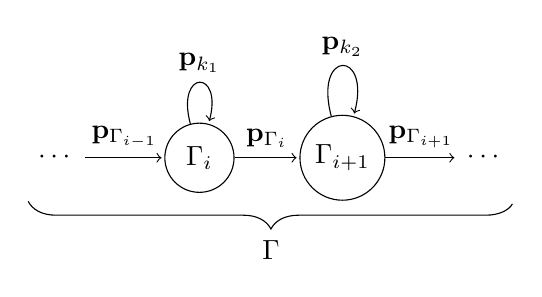
\begin{tikzpicture}[shorten >=1pt,node distance=12ex,on grid,auto] 
    \node        (q_dots0) {$\cdots$};
    \node[state] (q_0) [right=of q_dots0] {$\Gamma_i$};
    \node[state] (q_1) [right=of q_0] {$\Gamma_{i+1}$};
    \node        (q_dots1) [right=of q_1] {$\cdots$};   
    \path[->]
    (q_dots0) edge node{$\mathbf{p}_{\Gamma_{i-1}}$} (q_0)
    (q_0) edge node {$\mathbf{p}_{\Gamma_i}$} (q_1)    
    (q_0) edge [loop above] node {$\mathbf{p}_{k_1}$} (q_0)
    (q_1) edge node {$\mathbf{p}_{\Gamma_{i+1}}$} (q_dots1)
    (q_1) edge [loop above] node {$\mathbf{p}_{k_2}$} (q_1)
    ; %end path 
    \draw [decorate,decoration={brace,amplitude=10pt,mirror,raise=10pt},yshift=0pt]
    (q_dots0.south west) -- (q_dots1.south east) node [black,midway,yshift=-8ex]{$\Gamma$};
  \end{tikzpicture}
  \caption{The plan defined as a FSM}
  \label{fig:state-machine}
\end{figure}

A slice of the plan in Figure~\ref{fig:state-machine} shows the transition between the stages with the FSM. The triggering point $\mathbf{p}_{\Gamma_{i-1}}$ allows the transition to stage $\Gamma_i$. The UAV remains in the stage with any generic point $\mathbf{p}_{k_1}$. It eventually enters the stage $\Gamma_{i+1}$ with the triggering point $\mathbf{p}_{\Gamma_i}$ and so on, until it reaches the final point.

\begin{figure}[h]
  \center
  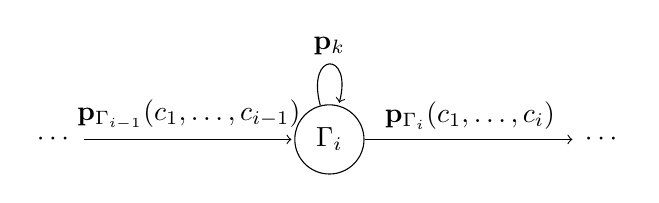
\begin{tikzpicture}[shorten >=1pt,node distance=23ex,on grid,auto] 
    \node        (q_dots0) {$\cdots$};
    \node[state] (q_0) [right=of q_dots0] {$\Gamma_i$};
    \node        (q_dots1) [right=of q_0] {$\cdots$};   
    \path[->]
    (q_dots0) edge node{$\mathbf{p}_{\Gamma_{i-1}}(c_1,\dots,c_{i-1})$} (q_0)
    (q_0) edge node {$\mathbf{p}_{\Gamma_i}(c_1,\dots,c_{i})$} (q_dots1)    
    (q_0) edge [loop above] node {$\mathbf{p}_{k}$} (q_0)
    ; %end path
  \end{tikzpicture}
  \caption{Detail of the stage $\Gamma_i$ in the FSM}
  \label{fig:state-machine2}
\end{figure}

Generally, one can express the triggering points in function of the $i$-th trajectory parameters $c_{i,1},\dots,c_{i,\rho}$, or any previous trajectory parameters, propagating the information therein if necessary. We show this in Figure~\ref{fig:state-machine2}, where, for simplicity, we neglected the $\sigma=0$ computations parameters, so $c_i=c_{i,1},\dots,c_{i,\rho}$.

We refer the reader to an example in Appendix~\ref{app:plan-example} for a detailed implementation. In the example, the first trajectory parameter is propagated to all the following trajectories and triggering points. 

We store the initial plan in the plan specification, the format is described in Appendix~\ref{app:plan-spec}. 

\subsection{Problem formulation}

In order to formulate the problem, we considerate the next assumption.

\begin{assm}[Plan periodicity]\label{assm:periodic}
  Given an initial plan $\Gamma$ consisting of $l$ stages, a generic starting point $\mathbf{p}$, the current levels of the parameters $c_{1,1},\dots,c_{1,\rho}$, and a shift $\mathbf{d}:=(x_d,y_d)$, there exists a constant $n\in\mathbb{Z}_{>0}$ ($n<l,l/n\in\mathbb{Z}$) such that
  \begin{equation*}\begin{split}
    &\varphi_{(i-1)n+j}(\mathbf{p}+(i-1)\mathbf{d},c_1)\approx\\ &\,\,\,\varphi_{in+j}(\mathbf{p}+i\mathbf{d},c_1),\,\,\,\forall i\in[l/n-1]^+,j\in[n]^+.
  \end{split}\end{equation*}
\end{assm}

Physically, this means that the plan is approximately periodic. We will see the assumption being eased for non-periodic plans in Section~\ref{sec:experimental}.

\begin{defn}[Period]\label{def:period}
  The period $T\in\mathbb{R}_{> 0}$ is defined as the time between $\varphi_{(i-1)n+j}$ and $\varphi_{in+j}$ in Assumption~\ref{assm:periodic}.
\end{defn}

The algorithm measures the time between the stages and assumes the initial period is one. We note that periods might be different for different $j$s due to atmospheric interferences. 

From Assumption~\ref{assm:periodic} follows the next proposition.

\begin{prop}[Necessary and sufficient condition for periodicity]\label{prop:rank}
  Suppose Assumption~\ref{assm:periodic} holds, then the plan $\Gamma$ is periodic if
  \begin{equation*}\begin{split}
    &\varphi_{(i-1)n+j}(\mathbf{p}+(i-1)\mathbf{d},c_1)-\\ &\,\,\,\varphi_{in+j}(\mathbf{p}+i\mathbf{d},c_1)=d_j,\,\,\,\forall i\in[l/n-1]^+,j\in[n]^+.
  \end{split}\end{equation*}
  Moreover, if the plan $\Gamma$ is periodic then
  \begin{equation*}
    \mathrm{rank}\begin{bmatrix}
        \varphi_1 & \varphi_{n+1} & \cdots & \varphi_{(l-n)+1} \\ 
        %\varphi_2 & \varphi_{n+2} & \cdots & \varphi_{(l-n)+2} \\
        \vdots & \vdots & \ddots & \vdots \\
        \varphi_n & \varphi_{2n} & \cdots & \varphi_l   
      \end{bmatrix}=2,
  \end{equation*}
  where the trajectories in the first column are evaluated  on $\mathbf{p},c_1$, in the second on $\mathbf{p}+\mathbf{d},c_1$, and in the last on $\mathbf{p}+(l/n-1)\mathbf{d},c_1$.
\end{prop}
\begin{proof}($\Longrightarrow$) The expression implies that $\varphi_{(i-1)n+j}$ is the same but shifted function in space $\varphi_{(i-1)n+j}=\varphi_{in+j}+d_j$ and $d_j$ is the $j$-th constant difference. This is equivalent to Assumption~\ref{assm:periodic}.
  
($\Longleftarrow$) The column rank of the matrix in the proposition is the dimension of its column space. It denotes the size of the set of all the possible linear combination of the column vectors. We note that there is a limited number (two) of linear combinations of the column vectors being these linearly dependent (from $\Longrightarrow$). 
\end{proof}

The proposition is a necessary ($\Longleftarrow$) and sufficient ($\Longrightarrow$) condition for the periodicity. The algorithm finds $n$ initializing it to one and finding the value which satisfies the proposition. 

\begin{pb}[UAV planning problem]\label{pb}
  Consider an initial plan $\Gamma$ defined in Definition~\ref{def:mission} that satisfies Assumption~\ref{assm:periodic}. We are interested in the planning of the path parameters $c_{i,1},\dots,c_{i,\rho}$ and computations parameters $c_{i,\rho+1},\dots,c_{i,\rho+\sigma}$ and in the guidance to the path resulting from such plan for the UAV planning problem.
\end{pb}


\section{Periodic Energy Model}
\label{sec:energy-model}

We model the energy using energy coefficients $\mathbf{q}\in\mathbb{R}^m$ that characterize the energy signal. We refer to the instantaneous energy consumption evolution simply as the energy signal. The coefficients are derived from Fourier analysis (the size of the energy coefficients vector $m$ is related to the order of a Fourier series) and estimated using a state estimator (Kalman filter). 

We proof a relation between the energy signal and the energy coefficients in Lemma~\ref{lem:eqv}. We show after the main results how this approach allows us variability in terms of the systems behaving periodically, piece-wise periodically, or merely linearly with sporadic periodicity.

Once we illustrate the energy model, we enhance it with the energy contribution of the trajectory in Subsection~\ref{sec:model}, and of the computations in Subsection~\ref{sec:computations-model}. 

Let us consider a periodic signal of period $T$, and a Fourier series of an arbitrary order $r\in\mathbb{Z}_{\geq 0}$ for the purpose of modeling of the energy signal
\begin{equation}\label{eq:fourier}
  h(t)=a_0/T+(2/T)\sum_{j=1}^{r}{\left(a_j\cos{\omega jt}+b_j\sin{\omega jt}\right)},
\end{equation}
where $h:\mathbb{R}_{\geq 0}\rightarrow\mathbb{R}$ maps time to the instantaneous energy consumption, $\omega:=2\pi/T$ is the angular frequency, and $a,b\in\mathbb{R}$ the Fourier series coefficients.

The energy signal can be modeled by Equation~(\ref{eq:fourier}) and by the output of a linear model
\begin{equation}\label{eq:state-perf}\begin{split}
  \dot{\mathbf{q}}&=A\mathbf{q}+B\mathbf{u},\\
  y&=C\mathbf{q},
\end{split}\end{equation}
where $y\in\mathbb{R}$ is the instantaneous energy consumption. 

The state $\mathbf{q}$ are the energy coefficients
\begin{equation}\label{eq:state-details}\begin{split}
  \mathbf{q}&=\left[\begin{array}{cccccc}
    \alpha_0 & \alpha_1 & \beta_1 & \cdots & \alpha_r & \beta_r
  \end{array}\right]^T,\\
  A&=\left[\begin{array}{cccc}
    0&    &       &  \\
     & A_1&       &  \\
     &    & \ddots&  \\
     &    &       & A_r 
  \end{array}\right],\,A_j\begin{bmatrix}0 & \omega j \\ -\omega j & 0\end{bmatrix},\\
  C&=(1/T)\left[\begin{array}{cccccc}
    1 & 1 & 0 &\cdots & 1 & 0
  \end{array}\right],
\end{split}\end{equation}
where $\mathbf{q}\in\mathbb{R}^m$ with $m=2r+1$, $A\in\mathbb{R}^{m\times m}$ is the state transmission matrix, and $C\in\mathbb{R}^m$ is the output matrix. In matrix $A$, the top left entry is zero, the diagonal entries are $A_1,\dots,A_r$, the remaining entries are zeros.

The linear model in Equation~(\ref{eq:state-perf}) allows us to include the control in the model of Equation~(\ref{eq:fourier}). In fact, the algorithm uses the model to find the control sequence that results in the optimal parameters configuration (using MPC). 

\begin{lem}[Signals equality]\label{lem:eqv}Suppose control is zero, matrices $A,C$ are described by Equation~(\ref{eq:state-details}), and the initial guess $\mathbf{q}_0$ is 
  \begin{equation*}
  \mathbf{q}_0=\begin{bmatrix}a_0 & a_1/2 & b_1/2 & \cdots & a_r/2 & b_r/2\end{bmatrix}^T.
  \end{equation*} 
  Then, the signal $h$ in Equation~(\ref{eq:fourier}) is equal to the output $y$ in Equation~(\ref{eq:state-perf}).
\end{lem}
\begin{proof}
The equivalence of the models is trivial and the equality of the signal and output is achieved by a proper choice of items of matrices $A,C$ and the initial guess $\mathbf{q}_0$. We refer the reader to Appendix~\ref{app:proof-eqv} for a formal proof of the equality where we justify the choices of the items of the matrices and of the initial guess. 
\end{proof}

Let us consider the discretized version $A_d:=A\Delta t+I$ of the matrix $A$. We denote the continuous and discrete time with the standard notation $t,k$. We use the forward Euler approximation with a small enough value of the time step $\Delta t$. We note that one can guarantee to have the same outputs rather than an approximation with $A_d:=e^{At}$.

Let us suppose that at time instant $k$ the plan reached the $i$-th stage $\Gamma_i$.

The control along with the input matrix
\begin{equation}\label{eq:state-control}\begin{split}
  \mathbf{u}_k&=\begin{bmatrix}c_{k,1} & \cdots & c_{k,\rho} & c_{k,\rho+1} & \cdots & c_{k,\rho+\sigma}\end{bmatrix}^T,\\
  B\mathbf{u}&:=B_i(\mathbf{u}_k-\mathbf{u}_{k-1}),\,\,\,B_i=\left[\begin{array}{c} \nu_i\\\mathbf{0}\end{array}\right],
\end{split}\end{equation}
where $\mathbf{u}\in\mathbb{R}^n$ is the control with $n=\rho+\sigma$, $B\in\mathbb{R}^{m\times n}$, and $\mathbf{u}_{-1}=\mathbf{0}$. Moreover, the top row of $B$ contains gain factors $\nu_i=\begin{bmatrix}\nu_{i,1} & \cdots & \nu_{i,\rho} & \nu_{i,\rho + 1}& \cdots & \nu_{i,\rho+\sigma}\end{bmatrix}$, quantifying the contribution of a given parameter to the instantaneous energy consumption. The other entries of $B$ are zeros. 

The first $\rho$ gain factors quantifies the contribution of the $i$-th trajectory parameters. A first guess of these parameters is derived empirically. They are later refined by the algorithm. The following $\sigma$ gain factors quantifies the contribution of the computations parameters. They are derived using the modeling tool. 

\subsection{Trajectory parameters energy contribution}
\label{sec:model}

\begin{figure}[h]
  \centering
  
\definecolor{c2B2B2B}{RGB}{43,43,43}
\definecolor{cDEDEDE}{RGB}{222,222,222}
\definecolor{c989898}{RGB}{152,152,152}
\definecolor{cFFFFFF}{RGB}{255,255,255}
\definecolor{c4D4D4D}{RGB}{77,77,77}
\definecolor{c9B9B9B}{RGB}{155,155,155}


\def \globalscale {1.000000}
\begin{tikzpicture}[y=0.80pt, x=0.80pt, yscale=-\globalscale, xscale=\globalscale, inner sep=0pt, outer sep=0pt]
\path[fill=c2B2B2B,line join=round,line width=0.256pt] (101.0350,53.6179) -- (96.2027,55.8748) -- (95.7468,54.6788) -- (100.5790,52.4218) -- (101.0350,53.6179) -- cycle(111.1420,50.5445) -- (106.0290,52.0626) -- (105.7610,50.8111) -- (110.8730,49.2930) -- (111.1420,50.5445) -- cycle;



\path[draw=c2B2B2B,line join=round,line width=1.024pt] (128.3820,48.6757) .. controls (127.0480,48.5917) and (125.7060,48.5494) .. (124.3560,48.5494) .. controls (119.7720,48.5494) and (115.2670,49.0390) .. (110.8680,49.9835);



  \path[fill=cDEDEDE,line join=round,even odd rule,line width=0.160pt] (201.2220,113.9290) .. controls (207.0530,111.9750) and (213.0250,110.6150) .. (219.4860,110.5010) -- (219.4860,142.5600) .. controls (204.1730,143.1220) and (191.8220,155.2870) .. (190.9640,170.5230) -- (190.9770,183.1500) -- (190.9640,183.4360) -- (190.9640,183.7260) .. controls (190.9770,184.4540) and (191.0820,185.2110) .. (191.0620,185.9270) -- (191.0670,185.9340) -- (191.0670,187.7060) -- (190.9640,227.8200) -- (190.9640,235.0380) -- (190.9450,235.0380) -- (190.9450,235.1810) -- (190.9340,235.9910) -- (190.9920,239.6820) -- (173.2000,239.6860) .. controls (173.4790,219.6570) and (172.4790,191.1610) .. (173.3370,172.5260) .. controls (173.7560,163.4250) and (175.7760,156.4540) .. (176.3670,154.3980) .. controls (178.5870,146.6790) and (177.0030,123.9390) .. (200.7770,114.0980) -- (201.2220,113.9290) -- cycle;



  \path[draw=c989898,line join=round,line width=0.512pt] (220.5790,172.1070) ellipse (1.7421cm and 1.7421cm);



  \path[draw=black,line join=round,line width=0.512pt] (222.7480,174.1440) -- (218.4670,169.8620);



  \path[draw=c2B2B2B,line join=round,line width=0.512pt] (283.0110,95.4499) -- (283.0100,239.6230);



  \path[draw=black,line join=round,line width=1.024pt] (212.5660,111.2220) .. controls (214.2910,110.4830) and (220.9040,110.5350) .. (220.9040,110.5350) .. controls (254.9950,110.5350) and (282.6310,138.1720) .. (282.6310,172.2630);



  \path[draw=black,line join=round,line width=0.512pt] (218.4680,174.1410) -- (222.7490,169.8600);



    \path[fill=cFFFFFF,line join=round,line width=0.160pt] (289.4020,105.0980) -- (276.9530,105.0980) -- (276.9530,121.0670) -- (289.4080,121.0670) -- (289.4020,105.0980) -- cycle;



    \path[cm={{1.0,0.0,0.0,1.0,(273.0,118.0)}}] (0.0000,0.0000) node[above right] () {$\varphi_{12}$};



  \path[draw=black,line join=round,line width=1.024pt] (282.6300,239.6340) -- (282.6300,172.0640);



  \path[draw=c2B2B2B,line join=round,line width=0.512pt] (221.1170,172.3260) ellipse (1.3451cm and 1.3451cm);



  \path[draw=c4D4D4D,line join=round,line width=0.512pt] (173.4260,95.3725) -- (173.4260,239.5460);



  \path[draw=black,line join=round,line width=0.512pt] (265.2780,189.1390) -- (220.7780,172.0720);



  \path[draw=black,line join=round,line width=1.024pt] (212.0450,110.8620) .. controls (176.5020,117.4390) and (178.8960,145.6300) .. (176.3720,154.4050) .. controls (173.7630,163.4760) and (173.3650,171.9460) .. (173.3650,171.9460) -- (173.3790,172.2110) -- (173.4210,172.6590);



  \path[draw=black,fill=c9B9B9B,line join=round,line width=0.512pt] (173.8510,165.3770) -- (181.8430,152.9480) -- (176.6230,153.7110) -- (172.6800,150.6460) -- (173.8510,165.3770) -- cycle;



  \path[fill=black,line join=round,line width=0.256pt] (172.7330,229.2390) -- (172.7330,223.9060) -- (174.0130,223.9060) -- (174.0130,229.2390) -- (172.7330,229.2390) -- cycle(172.7330,218.5730) -- (172.7330,213.2390) -- (174.0130,213.2390) -- (174.0130,218.5730) -- (172.7330,218.5730) -- cycle(172.7330,207.9060) -- (172.7330,202.5730) -- (174.0130,202.5730) -- (174.0130,207.9060) -- (172.7330,207.9060) -- cycle(172.7330,197.2390) -- (172.7330,191.9060) -- (174.0130,191.9060) -- (174.0130,197.2390) -- (172.7330,197.2390) -- cycle(172.7330,186.5730) -- (172.7330,181.2390) -- (174.0130,181.2390) -- (174.0130,186.5730) -- (172.7330,186.5730) -- cycle(172.7330,175.9060) -- (172.7330,172.3360) -- (174.0130,172.3360) -- (174.0130,175.9060) -- (172.7330,175.9060) -- cycle(172.7330,239.9060) -- (172.7330,234.5730) -- (174.0130,234.5730) -- (174.0130,239.9060) -- (172.7330,239.9060) -- cycle;



    \path[fill=cFFFFFF,line join=round,line width=0.160pt,rounded corners=0.0000cm] (167.3680,105.0980) rectangle (179.8176,121.0676);



    \path[cm={{1.0,0.0,0.0,1.0,(164.0,118.0)}}] (0.0000,0.0000) node[above right] () {$\varphi_{14}^-$};



    \path[fill=cFFFFFF,line join=round,line width=0.160pt] (177.5750,234.3400) -- (165.1260,234.3400) -- (165.0920,246.4150) -- (177.5710,246.3840) -- (177.5750,234.3400) -- cycle;



    \path[cm={{1.0,0.0,0.0,1.0,(164.0,245.0)}}] (0.0000,0.0000) node[above right] () {$\overline{c}_{14}^-$};



    \path[fill=cFFFFFF,line join=round,line width=0.160pt,rounded corners=0.0000cm] (230.3230,173.2320) rectangle (251.5725,189.2016);



    \path[cm={{1.0,0.0,0.0,1.0,(232.0,185.0)}}] (0.0000,0.0000) node[above right] () {$c_{1,1}^-$};



  \path[draw=black,fill=cFFFFFF,line join=round,line width=0.512pt] (203.3560,114.4210) -- (218.0050,112.4770) -- (213.5600,109.7230) -- (213.8340,104.0000) -- (203.3560,114.4210) -- cycle;



    \path[fill=cFFFFFF,line join=round,line width=0.160pt] (199.4770,144.8830) -- (183.5080,144.8830) -- (183.5080,160.8530) -- (199.4770,160.8530) -- (199.4770,144.8830) -- cycle;



    \path[cm={{1.0,0.0,0.0,1.0,(185.0,158.0)}}] (0.0000,0.0000) node[above right] () {$\mathbf{p}_{k_6}$};

    \path[cm={{1.0,0.0,0.0,1.0,(161.0,170.0)}}] (0.0000,0.0000) node[above right] () {\ref{sth:iii}};

    \path[fill=cFFFFFF,line join=round,line width=0.160pt,rounded corners=0.0000cm] (192.4050,96.8819) rectangle (204.8546,109.3314);


  \path[draw=black,line join=round,line width=0.512pt] (203.7170,114.2570) -- (213.5160,109.7120);



  \path[draw=black,line join=round,line width=0.512pt] (174.0250,164.7330) -- (176.5840,153.7760);



    \path[fill=cFFFFFF,line join=round,line width=0.160pt] (219.2260,208.5700) -- (203.2560,208.5700) -- (203.2560,224.5400) -- (219.2260,224.5390) -- (219.2260,208.5700) -- cycle;



    \path[cm={{1.0,0.0,0.0,1.0,(202.0,222.0)}}] (0.0000,0.0000) node[above right] () {$\varphi_{13}^-$};



  \path[draw=c989898,line join=round,line width=0.512pt] (158.8570,95.3893) -- (158.8570,239.5620);



  \path[cm={{1.0,0.0,0.0,1.0,(181.0,261.0)}}] (0.0000,0.0000) node[above right] () {\footnotesize (b) replanned path};



  \path[fill=black,line join=round,line width=0.160pt] (262.5930,185.4440) -- (260.7610,189.7900) -- (265.6570,189.2950) -- (262.5930,185.4440) -- cycle;



\path[draw=c2B2B2B,line join=round,line width=0.512pt] (137.9100,95.3391) -- (137.9100,239.5120);



  \path[fill=cFFFFFF,line join=round,line width=0.160pt] (144.6860,105.0630) -- (131.2360,105.0630) -- (131.2360,121.0330) -- (144.6960,121.0670) -- (144.6860,105.0630) -- cycle;



  \path[cm={{1.0,0.0,0.0,1.0,(128.0,118.0)}}] (0.0000,0.0000) node[above right] () {$\varphi_{12}$};



\path[fill=cDEDEDE,line join=round,line width=0.160pt] (14.4062,169.9360) -- (14.4311,169.9360) .. controls (15.3584,137.0320) and (42.0351,110.5710) .. (75.0243,109.9900) -- (75.0243,142.0480) .. controls (59.7109,142.6110) and (47.3600,154.7750) .. (46.5019,170.0120) -- (46.5148,182.6390) -- (46.5019,182.9250) -- (46.5019,183.2150) .. controls (46.5154,183.9430) and (46.6203,184.7000) .. (46.6001,185.4160) -- (46.6055,185.4230) -- (46.6055,187.1950) -- (46.5019,227.3090) -- (46.5019,234.5270) -- (46.4833,234.5270) -- (46.4830,234.6700) -- (46.4723,235.4800) -- (46.5303,239.1710) -- (14.2304,239.1780) .. controls (14.2304,237.5050) and (14.2092,240.8130) .. (14.1991,237.1110) -- (14.1991,235.5690) -- (14.1991,235.2560) -- (14.1991,234.8370) -- (14.1991,234.5320) -- (14.1991,171.8980) -- (14.4062,169.9360) -- cycle;



\path[draw=c2B2B2B,line join=round,line width=0.512pt] (75.8516,172.0930) ellipse (1.7421cm and 1.7421cm);



\path[draw=black,line join=round,line width=0.512pt] (78.0152,174.1270) -- (73.7395,169.8460);



\path[draw=black,line join=round,line width=0.512pt] (73.7417,174.1270) -- (78.0230,169.8460);



\path[draw=c2B2B2B,line join=round,line width=0.512pt] (14.1483,95.3578) -- (14.1477,239.5310);



\path[draw=black,line join=round,line width=0.512pt] (75.9234,172.0190) -- (14.0743,172.0190);



\path[fill=black,line join=round,line width=0.160pt] (19.0789,174.3350) -- (19.0727,169.6190) -- (14.7563,171.9820) -- (19.0789,174.3350) -- cycle;



  \path[fill=cFFFFFF,line join=round,line width=0.160pt,rounded corners=0.0000cm] (8.0901,105.0980) rectangle (20.5396,121.0676);



  \path[cm={{1.0,0.0,0.0,1.0,(5.0,118.0)}}] (0.0000,0.0000) node[above right] () {$\varphi_{14}$};



\path[draw=black,line join=round,line width=1.024pt] (67.5256,111.0380) .. controls (69.2504,110.2990) and (75.8630,110.3510) .. (75.8630,110.3510) .. controls (109.9540,110.3510) and (137.5900,137.9880) .. (137.5900,172.0790);



  \path[fill=cFFFFFF,line join=round,line width=0.160pt,rounded corners=0.0000cm] (115.2640,126.2090) rectangle (131.2335,138.6585);



  \path[cm={{1.0,0.0,0.0,1.0,(114.0,137.0)}}] (0.0000,0.0000) node[above right] () {$\varphi_{13}$};



  \path[fill=cFFFFFF,line join=round,line width=0.160pt] (52.6996,234.3410) -- (40.2501,234.3410) -- (40.2318,246.3700) -- (52.7105,246.3700) -- (52.6996,234.3410) -- cycle;



  \path[cm={{1.0,0.0,0.0,1.0,(44.0,245.0)}}] (0.0000,0.0000) node[above right] () {$\underline{c}_{14}$};



  \path[fill=cFFFFFF,line join=round,line width=0.160pt] (64.6687,169.3940) -- (46.9391,169.3930) -- (46.9391,181.8430) -- (64.6687,181.8430) -- (64.6687,169.3940) -- cycle;



  \path[cm={{1.0,0.0,0.0,1.0,(47.0,181.0)}}] (0.0000,0.0000) node[above right] () {$c_{1,1}$};



\path[fill=black,line join=round,line width=0.256pt] (13.8207,228.7410) -- (13.8435,223.4080) -- (15.1234,223.4140) -- (15.1007,228.7470) -- (13.8207,228.7410) -- cycle(13.8662,218.0750) -- (13.8890,212.7420) -- (15.1690,212.7470) -- (15.1462,218.0800) -- (13.8662,218.0750) -- cycle(13.9117,207.4080) -- (13.9345,202.0750) -- (15.2145,202.0800) -- (15.1917,207.4140) -- (13.9117,207.4080) -- cycle(13.9572,196.7420) -- (13.9800,191.4080) -- (15.2600,191.4140) -- (15.2372,196.7470) -- (13.9572,196.7420) -- cycle(14.0028,186.0750) -- (14.0255,180.7420) -- (15.3055,180.7470) -- (15.2828,186.0810) -- (14.0028,186.0750) -- cycle(14.0483,175.4090) -- (14.0711,170.0750) -- (15.3510,170.0810) -- (15.3283,175.4140) -- (14.0483,175.4090) -- cycle(14.0938,164.7420) -- (14.1004,163.1940) -- (14.1116,163.0700) -- (14.1481,162.9500) -- (14.2078,162.8390) -- (14.2888,162.7440) -- (14.3849,162.6630) -- (14.4954,162.6040) -- (14.6155,162.5680) -- (14.7404,162.5570) -- (14.1975,162.5580) -- (14.4982,161.0400) -- (14.8987,159.3600) -- (16.1499,159.6300) -- (15.7494,161.3100) -- (15.4579,162.7820) -- (14.7404,163.8370) -- (15.3804,163.2000) -- (15.3738,164.7470) -- (14.0938,164.7420) -- cycle(16.4171,154.1910) -- (17.1786,151.9470) -- (18.2993,149.1670) -- (19.5002,149.6100) -- (18.3795,152.3900) -- (17.6397,154.5700) -- (16.4171,154.1910) -- cycle(20.5366,144.2860) -- (20.9681,143.3850) -- (23.1393,139.5830) -- (24.2741,140.1750) -- (22.1029,143.9770) -- (21.7089,144.7990) -- (20.5366,144.2860) -- cycle(26.1128,135.1000) -- (26.8488,134.0250) -- (29.4547,130.8780) -- (30.4785,131.6470) -- (27.8725,134.7930) -- (27.1990,135.7770) -- (26.1128,135.1000) -- cycle(33.1525,126.9590) -- (35.2417,124.9010) -- (37.1822,123.3740) -- (38.0303,124.3330) -- (36.0897,125.8600) -- (34.0975,127.8220) -- (33.1525,126.9590) -- cycle(41.5104,120.1440) -- (46.0624,117.3650) -- (46.7947,118.4150) -- (42.2427,121.1940) -- (41.5104,120.1440) -- cycle(50.9592,115.0720) -- (53.4451,113.9480) -- (56.0106,113.1560) -- (56.4648,114.3530) -- (53.8993,115.1450) -- (51.5589,116.2030) -- (50.9592,115.0720) -- cycle(61.1063,111.5820) -- (61.2085,111.5500) -- (66.4314,110.6160) -- (66.7338,111.8590) -- (61.5109,112.7940) -- (61.5606,112.7790) -- (61.1063,111.5820) -- cycle(13.7752,239.4080) -- (13.7979,234.0750) -- (15.0779,234.0800) -- (15.0552,239.4130) -- (13.7752,239.4080) -- cycle;



\path[cm={{1.0,0.0,0.0,1.0,(43.0,110.0)}}] (0.0000,0.0000) node[above right] () {$\mathbf{p}_{k_5}$};

\path[cm={{1.0,0.0,0.0,1.0,(72.0,105.0)}}] (0.0000,0.0000) node[above right] () {\ref{sth:i}};

  \path[fill=cFFFFFF,line join=round,line width=0.160pt] (18.9147,234.3410) -- (6.4652,234.3410) -- (6.4316,246.4160) -- (18.9102,246.3850) -- (18.9147,234.3410) -- cycle;



  \path[cm={{1.0,0.0,0.0,1.0,(6.0,245.0)}}] (0.0000,0.0000) node[above right] () {$\overline{c}_{14}$};



\path[draw=black,fill=c9B9B9B,line join=round,line width=0.512pt] (58.9895,114.4960) -- (73.6370,112.5410) -- (69.1896,109.7900) -- (69.4587,104.0670) -- (58.9895,114.4960) -- cycle;



\path[draw=black,line join=round,line width=0.512pt] (59.2931,114.3470) -- (69.0932,109.8070);



\path[cm={{1.0,0.0,0.0,1.0,(37.0,261.0)}}] (0.0000,0.0000) node[above right] () {\footnotesize (a) initial path};



\path[draw=black,line join=round,line width=1.024pt] (137.5900,239.4500) -- (137.5900,171.8800);



\path[fill=cDEDEDE,line join=round,even odd rule,line width=0.160pt] (237.0260,15.0828) -- (265.6100,15.0831) -- (265.6100,33.6677) -- (237.0260,33.6675) -- (237.0260,15.0828) -- cycle;



\path[cm={{1.0,0.0,0.0,1.0,(274.0,29.0)}}] (0.0000,0.0000) node[above right] () {$\mathcal{P}_i$};



\path[draw=black,line join=round,line width=1.024pt] (237.0260,52.5827) -- (265.6110,52.5829);



\path[cm={{1.0,0.0,0.0,1.0,(274.0,56.0)}}] (0.0000,0.0000) node[above right] () {$\mathcal{P}$};



\path[draw=black,fill=c9B9B9B,line join=round,line width=0.512pt] (103.0020,54.8369) -- (121.9910,51.9150) -- (117.5520,47.3939) -- (116.3400,41.0080) -- (103.0020,54.8369) -- cycle;



\path[draw=black,line join=round,line width=0.512pt] (115.1520,48.6445) -- (111.3670,18.4898);



\path[draw=black,line join=round,line width=0.512pt] (115.2340,48.4465) -- (94.3696,72.9709);



\path[cm={{1.0,0.0,0.0,1.0,(102.0,15.0)}}] (0.0000,0.0000) node[above right] () {$\nabla\varPhi$};



\path[cm={{1.0,0.0,0.0,1.0,(96.0,86.0)}}] (0.0000,0.0000) node[above right] () {$\dot{\mathbf{p}}$};



\path[cm={{1.0,0.0,0.0,1.0,(79.0,45.0)}}] (0.0000,0.0000) node[above right] () {$\dot{\mathbf{p}}_d$};



\path[draw=black,line join=round,line width=0.512pt] (117.5520,47.3796) -- (103.1340,54.7265);



\path[fill=black,line join=round,line width=0.160pt] (99.4724,72.0401) -- (94.9925,67.8546) -- (93.3980,74.0506) -- (99.4724,72.0401) -- cycle;



\path[fill=black,line join=round,line width=0.160pt] (108.7830,21.3255) -- (114.8390,20.3742) -- (110.9400,15.3018) -- (108.7830,21.3255) -- cycle;



\path[fill=black,line join=round,line width=0.160pt] (79.6380,52.9767) -- (85.2585,55.4260) -- (84.6922,49.0532) -- (79.6380,52.9767) -- cycle;



\path[draw=black,line join=round,line width=0.512pt] (82.5181,52.4879) -- (114.8620,48.5042);



\path[draw=black,line join=round,line width=0.512pt] (40.3847,53.3572) -- (62.7169,53.3572);



\path[cm={{1.0,0.0,0.0,1.0,(47.0,50.0)}}] (0.0000,0.0000) node[above right] () {$w$};



\path[fill=black,line join=round,line width=0.160pt] (61.8249,50.0137) -- (61.8330,56.1447) -- (67.4450,53.0723) -- (61.8249,50.0137) -- cycle;




\end{tikzpicture}


  \caption{Illustrative figure shows the alteration of the trajectory parameter $c_{1,1}$, the radius of the circle (the alteration of the path from Figure~\ref{fig:il-abs}).}
  \label{fig:tee1}
\end{figure}

Equation~(\ref{eq:state-control}) accounts for the energy due to the change of parameters $\mathbf{u}_k-\mathbf{u}_{k-1}$. For instance, when the trajectory $\varphi_1$ is a circle (see Figure~\ref{fig:tee1}), a decrement in the trajectory parameter $c_{1,1}$--the radius of the circle--adds a negative contribution. It thus simulates the lowering of instantaneous energy consumption $\nu_{1,1}(c_{1,1}-c_{1,1}^-)<0$, for a given $\nu_{1,1}\in\mathbb{R}_{<0}$. This is then summed to the first coefficient $\alpha_0$, shifting the modeled energy.

Let us assume that the set
\begin{equation}\label{eq:area}
  \mathcal{P}_i:=\{\mathbf{p}_k\mid\varphi_i(\mathbf{p}_k,c_{i,1},\dots,c_{i,\rho})\in\mathcal{C}_i\},
\end{equation}
delimits the area where the $i$-th trajectory $\varphi_i$ is free to evolve using the trajectory parameters $c_{i,1},...,c_{i,\rho}$ (the gray area in Figure~\ref{fig:tee1}). $\varphi_i$ is a function of the two coordinates and is equal to zero when a point $\mathbf{p}_k$ is on the trajectory. Physically, this means the UAV is flying exactly over the nominal trajectory. The trajectory parameters allows to change the trajectory. They are a way to alter the nominal trajectory in the initial plan and thus alter the energy signal.
In fact, the algorithm uses the set from Equation~(\ref{eq:area}) to find the optimal trajectory parameters $c_i^0$ (here we again neglect for simplicity the $\sigma=0$ computations parameters), such that $\varphi_i(\mathbf{p}_k,c_i^0)$ has the highest instantaneous energy consumption (while still respecting the energy budget). The sequence of these parameters (control sequence) forms the path $\mathcal{P}$.

We derive the new position $\mathbf{p}_{k+1}$ using the function $\varPhi:=\varphi_i(\mathbf{p}_k,\mathbf{c}_i^0)$, computing its vector field $\nabla\varPhi:=\begin{bmatrix}\partial\varPhi/\partial x & \partial\varPhi/\partial y\end{bmatrix}^T$, and the direction to follow in the form of velocity vector~\cite{de2017guidance}
\begin{equation*}\label{eq:pd}
  \dot{\mathbf{p}}_d(\mathbf{p}_k):=E\nabla\varPhi-k_e\varPhi\nabla\varPhi,\,\,\,E=\begin{bmatrix}
    0&1\\-1&0
  \end{bmatrix},
\end{equation*}
where $E$ specifies the rotation (which influence the tracking direction), and $k_e\in\mathbb{R}_{\geq 0}$ the gain to adjusts the speed of convergence. The direction the velocity vector $\dot{\mathbf{p}}_d$ is pointing at is generally different from the course heading $\dot{\mathbf{p}}$ due to the atmospheric interferences, such as wind ($w\in\mathbb{R}$ in Figure~\ref{fig:tee1}).

\subsection{Computations parameters energy contribution}
\label{sec:computations-model}

Let us recall from Definition~\ref{def:mission} that the $i$-th stage $\Gamma_i$ of the plan $\Gamma$ contains the computations parameters which characterize the computations. We assess the energy cost of these computations using \powprof{}, the open-source modeling tool adapted from earlier work on computational energy analysis~\cite{seewald2019coarse, seewald2019component}, and energy estimation of a fixed-wing UAV~\cite{seewald2020mechanical}. 

We assume the UAV carries an embedded board that runs the computations. The tool measures the instantaneous energy consumption of a subset of possible computations parameters within the computations constraints sets and builds an energy model: a linear interpolation, one per each computation. 

The computations are implemented by software components, such as ROS nodes in a ROS based system. The user implements these nodes in such a way that they change the computational load with node-specific ROS parameters, the computations parameters. In a generic software component system, the user maps the computational load to the arguments. In both cases, with ROS~\cite{zamanakos2020energy} or with generic software components system~\cite{seewald2019component}, the tool performs automatic modeling. For instance, if the computation is a CNN object detector, the computation parameter $c_{i,\rho+1}$ corresponds to frames-per-second (fps) rate. The tool then changes the detection frequency.

We note that while the trajectory can differ for each stage, the tasks remain the same. However, the user can inhibit or enable a computation varying its computation set.

Let us further define $g:\mathbb{Z}_{\geq 0}\rightarrow\mathbb{R}_{\geq 0}$ as the instantaneous computational energy consumption value obtained using the tool.

The gain factors that quantifies the contribution of the computations parameters
\begin{equation*}\label{eq:energy-comp}
  \begin{bmatrix}\nu_{i,\rho+1} \\ \vdots \\ \nu_{i,\rho+\sigma}\end{bmatrix}^T=\begin{bmatrix}g(c_{i,\rho+1}) \\ \vdots \\ g(c_{i,\rho+\sigma})\end{bmatrix}/\begin{bmatrix}c_{i,\rho+1} & \cdots & c_{i,\rho+\sigma}\end{bmatrix}.
\end{equation*}
Moreover, let $g(\{\emptyset\})$ be zero.


\begin{figure*}
  \begin{tikzpicture}
    \node[inner sep=0pt] () at (0,7)
        {\footnotesize
\definecolor{ca0a0a4}{RGB}{160,160,164}
\definecolor{cffffff}{RGB}{255,255,255}
\definecolor{cff0000}{RGB}{255,0,0}


\def \globalscale {1.000000}
\begin{tikzpicture}[y=0.80pt, x=0.80pt, yscale=-\globalscale, xscale=\globalscale, inner sep=0pt, outer sep=0pt]
\begin{scope}[draw=black,line join=bevel,line cap=rect,even odd rule,line width=0.800pt]
  \begin{scope}[cm={{1.0,0.0,0.0,1.0,(0.0,0.0)}},draw=black,line join=bevel,line cap=rect,line width=0.800pt]
  \end{scope}
  \begin{scope}[cm={{1.00769,0.0,0.0,1.00769,(0.0,0.0)}},draw=black,line join=bevel,line cap=rect,line width=0.800pt]
  \end{scope}
  \begin{scope}[cm={{1.00769,0.0,0.0,1.00769,(0.0,0.0)}},draw=ca0a0a4,dash pattern=on 0.40pt off 0.80pt,line join=round,line cap=round,line width=0.400pt]
    \path[draw] (41.5000,109.5000) -- (140.5000,109.5000);



  \end{scope}
  \begin{scope}[cm={{1.00769,0.0,0.0,1.00769,(0.0,0.0)}},draw=black,line join=round,line cap=round,line width=0.480pt]
    \path[draw] (41.5000,109.5000) -- (44.5000,109.5000);



    \path[draw] (140.5000,109.5000) -- (137.5000,109.5000);



  \end{scope}
  \begin{scope}[cm={{1.00769,0.0,0.0,1.00769,(0.0,0.0)}},draw=black,line join=bevel,line cap=rect,line width=0.800pt]
  \end{scope}
  \begin{scope}[cm={{1.00769,0.0,0.0,1.00769,(15.1154,113.869)}},draw=black,line join=bevel,line cap=rect,line width=0.800pt]
  \end{scope}
  \begin{scope}[cm={{1.00769,0.0,0.0,1.00769,(15.1154,113.869)}},draw=black,line join=bevel,line cap=rect,line width=0.800pt]
  \end{scope}
  \begin{scope}[cm={{1.00769,0.0,0.0,1.00769,(15.1154,113.869)}},draw=black,line join=bevel,line cap=rect,line width=0.800pt]
  \end{scope}
  \begin{scope}[cm={{1.00769,0.0,0.0,1.00769,(15.1154,113.869)}},draw=black,line join=bevel,line cap=rect,line width=0.800pt]
  \end{scope}
  \begin{scope}[cm={{1.00769,0.0,0.0,1.00769,(15.1154,113.869)}},draw=black,line join=bevel,line cap=rect,line width=0.800pt]
  \end{scope}
  \begin{scope}[cm={{1.00769,0.0,0.0,1.00769,(15.1154,113.869)}},draw=black,line join=bevel,line cap=rect,line width=0.800pt]
    \path[fill=black] (0.0000,0.0000) node[above right] () {-100};



  \end{scope}
  \begin{scope}[cm={{1.00769,0.0,0.0,1.00769,(15.1154,113.869)}},draw=black,line join=bevel,line cap=rect,line width=0.800pt]
  \end{scope}
  \begin{scope}[cm={{1.00769,0.0,0.0,1.00769,(0.0,0.0)}},draw=black,line join=bevel,line cap=rect,line width=0.800pt]
  \end{scope}
  \begin{scope}[cm={{1.00769,0.0,0.0,1.00769,(0.0,0.0)}},draw=ca0a0a4,dash pattern=on 0.40pt off 0.80pt,line join=round,line cap=round,line width=0.400pt]
    \path[draw] (41.5000,84.5000) -- (140.5000,84.5000);



  \end{scope}
  \begin{scope}[cm={{1.00769,0.0,0.0,1.00769,(0.0,0.0)}},draw=black,line join=round,line cap=round,line width=0.480pt]
    \path[draw] (41.5000,84.5000) -- (44.5000,84.5000);



    \path[draw] (140.5000,84.5000) -- (137.5000,84.5000);



  \end{scope}
  \begin{scope}[cm={{1.00769,0.0,0.0,1.00769,(0.0,0.0)}},draw=black,line join=bevel,line cap=rect,line width=0.800pt]
  \end{scope}
  \begin{scope}[cm={{1.00769,0.0,0.0,1.00769,(31.2385,89.6846)}},draw=black,line join=bevel,line cap=rect,line width=0.800pt]
  \end{scope}
  \begin{scope}[cm={{1.00769,0.0,0.0,1.00769,(31.2385,89.6846)}},draw=black,line join=bevel,line cap=rect,line width=0.800pt]
  \end{scope}
  \begin{scope}[cm={{1.00769,0.0,0.0,1.00769,(31.2385,89.6846)}},draw=black,line join=bevel,line cap=rect,line width=0.800pt]
  \end{scope}
  \begin{scope}[cm={{1.00769,0.0,0.0,1.00769,(31.2385,89.6846)}},draw=black,line join=bevel,line cap=rect,line width=0.800pt]
  \end{scope}
  \begin{scope}[cm={{1.00769,0.0,0.0,1.00769,(31.2385,89.6846)}},draw=black,line join=bevel,line cap=rect,line width=0.800pt]
  \end{scope}
  \begin{scope}[cm={{1.00769,0.0,0.0,1.00769,(31.2385,89.6846)}},draw=black,line join=bevel,line cap=rect,line width=0.800pt]
    \path[fill=black] (0.0000,0.0000) node[above right] () {0};



  \end{scope}
  \begin{scope}[cm={{1.00769,0.0,0.0,1.00769,(31.2385,89.6846)}},draw=black,line join=bevel,line cap=rect,line width=0.800pt]
  \end{scope}
  \begin{scope}[cm={{1.00769,0.0,0.0,1.00769,(0.0,0.0)}},draw=black,line join=bevel,line cap=rect,line width=0.800pt]
  \end{scope}
  \begin{scope}[cm={{1.00769,0.0,0.0,1.00769,(0.0,0.0)}},draw=ca0a0a4,dash pattern=on 0.40pt off 0.80pt,line join=round,line cap=round,line width=0.400pt]
    \path[draw] (41.5000,59.5000) -- (140.5000,59.5000);



  \end{scope}
  \begin{scope}[cm={{1.00769,0.0,0.0,1.00769,(0.0,0.0)}},draw=black,line join=round,line cap=round,line width=0.480pt]
    \path[draw] (41.5000,59.5000) -- (44.5000,59.5000);



    \path[draw] (140.5000,59.5000) -- (137.5000,59.5000);



  \end{scope}
  \begin{scope}[cm={{1.00769,0.0,0.0,1.00769,(0.0,0.0)}},draw=black,line join=bevel,line cap=rect,line width=0.800pt]
  \end{scope}
  \begin{scope}[cm={{1.00769,0.0,0.0,1.00769,(19.1462,64.4923)}},draw=black,line join=bevel,line cap=rect,line width=0.800pt]
  \end{scope}
  \begin{scope}[cm={{1.00769,0.0,0.0,1.00769,(19.1462,64.4923)}},draw=black,line join=bevel,line cap=rect,line width=0.800pt]
  \end{scope}
  \begin{scope}[cm={{1.00769,0.0,0.0,1.00769,(19.1462,64.4923)}},draw=black,line join=bevel,line cap=rect,line width=0.800pt]
  \end{scope}
  \begin{scope}[cm={{1.00769,0.0,0.0,1.00769,(19.1462,64.4923)}},draw=black,line join=bevel,line cap=rect,line width=0.800pt]
  \end{scope}
  \begin{scope}[cm={{1.00769,0.0,0.0,1.00769,(19.1462,64.4923)}},draw=black,line join=bevel,line cap=rect,line width=0.800pt]
  \end{scope}
  \begin{scope}[cm={{1.00769,0.0,0.0,1.00769,(19.1462,64.4923)}},draw=black,line join=bevel,line cap=rect,line width=0.800pt]
    \path[fill=black] (0.0000,0.0000) node[above right] () {100};



  \end{scope}
  \begin{scope}[cm={{1.00769,0.0,0.0,1.00769,(19.1462,64.4923)}},draw=black,line join=bevel,line cap=rect,line width=0.800pt]
  \end{scope}
  \begin{scope}[cm={{1.00769,0.0,0.0,1.00769,(0.0,0.0)}},draw=black,line join=bevel,line cap=rect,line width=0.800pt]
  \end{scope}
  \begin{scope}[cm={{1.00769,0.0,0.0,1.00769,(0.0,0.0)}},draw=ca0a0a4,dash pattern=on 0.40pt off 0.80pt,line join=round,line cap=round,line width=0.400pt]
    \path[draw] (41.5000,35.5000) -- (140.5000,35.5000);



  \end{scope}
  \begin{scope}[cm={{1.00769,0.0,0.0,1.00769,(0.0,0.0)}},draw=black,line join=round,line cap=round,line width=0.480pt]
    \path[draw] (41.5000,35.5000) -- (44.5000,35.5000);



    \path[draw] (140.5000,35.5000) -- (137.5000,35.5000);



  \end{scope}
  \begin{scope}[cm={{1.00769,0.0,0.0,1.00769,(0.0,0.0)}},draw=black,line join=bevel,line cap=rect,line width=0.800pt]
  \end{scope}
  \begin{scope}[cm={{1.00769,0.0,0.0,1.00769,(19.1462,39.3)}},draw=black,line join=bevel,line cap=rect,line width=0.800pt]
  \end{scope}
  \begin{scope}[cm={{1.00769,0.0,0.0,1.00769,(19.1462,39.3)}},draw=black,line join=bevel,line cap=rect,line width=0.800pt]
  \end{scope}
  \begin{scope}[cm={{1.00769,0.0,0.0,1.00769,(19.1462,39.3)}},draw=black,line join=bevel,line cap=rect,line width=0.800pt]
  \end{scope}
  \begin{scope}[cm={{1.00769,0.0,0.0,1.00769,(19.1462,39.3)}},draw=black,line join=bevel,line cap=rect,line width=0.800pt]
  \end{scope}
  \begin{scope}[cm={{1.00769,0.0,0.0,1.00769,(19.1462,39.3)}},draw=black,line join=bevel,line cap=rect,line width=0.800pt]
  \end{scope}
  \begin{scope}[cm={{1.00769,0.0,0.0,1.00769,(19.1462,39.3)}},draw=black,line join=bevel,line cap=rect,line width=0.800pt]
    \path[fill=black] (0.0000,0.0000) node[above right] () {200};



  \end{scope}
  \begin{scope}[cm={{1.00769,0.0,0.0,1.00769,(19.1462,39.3)}},draw=black,line join=bevel,line cap=rect,line width=0.800pt]
  \end{scope}
  \begin{scope}[cm={{1.00769,0.0,0.0,1.00769,(0.0,0.0)}},draw=black,line join=bevel,line cap=rect,line width=0.800pt]
  \end{scope}
  \begin{scope}[cm={{1.00769,0.0,0.0,1.00769,(0.0,0.0)}},draw=ca0a0a4,dash pattern=on 0.40pt off 0.80pt,line join=round,line cap=round,line width=0.400pt]
    \path[draw] (41.5000,10.5000) -- (140.5000,10.5000);



  \end{scope}
  \begin{scope}[cm={{1.00769,0.0,0.0,1.00769,(0.0,0.0)}},draw=black,line join=round,line cap=round,line width=0.480pt]
    \path[draw] (41.5000,10.5000) -- (44.5000,10.5000);



    \path[draw] (140.5000,10.5000) -- (137.5000,10.5000);



  \end{scope}
  \begin{scope}[cm={{1.00769,0.0,0.0,1.00769,(0.0,0.0)}},draw=black,line join=bevel,line cap=rect,line width=0.800pt]
  \end{scope}
  \begin{scope}[cm={{1.00769,0.0,0.0,1.00769,(19.1462,15.1154)}},draw=black,line join=bevel,line cap=rect,line width=0.800pt]
  \end{scope}
  \begin{scope}[cm={{1.00769,0.0,0.0,1.00769,(19.1462,15.1154)}},draw=black,line join=bevel,line cap=rect,line width=0.800pt]
  \end{scope}
  \begin{scope}[cm={{1.00769,0.0,0.0,1.00769,(19.1462,15.1154)}},draw=black,line join=bevel,line cap=rect,line width=0.800pt]
  \end{scope}
  \begin{scope}[cm={{1.00769,0.0,0.0,1.00769,(19.1462,15.1154)}},draw=black,line join=bevel,line cap=rect,line width=0.800pt]
  \end{scope}
  \begin{scope}[cm={{1.00769,0.0,0.0,1.00769,(19.1462,15.1154)}},draw=black,line join=bevel,line cap=rect,line width=0.800pt]
  \end{scope}
  \begin{scope}[cm={{1.00769,0.0,0.0,1.00769,(19.1462,15.1154)}},draw=black,line join=bevel,line cap=rect,line width=0.800pt]
    \path[fill=black] (0.0000,0.0000) node[above right] () {300};



  \end{scope}
  \begin{scope}[cm={{1.00769,0.0,0.0,1.00769,(19.1462,15.1154)}},draw=black,line join=bevel,line cap=rect,line width=0.800pt]
  \end{scope}
  \begin{scope}[cm={{1.00769,0.0,0.0,1.00769,(0.0,0.0)}},draw=black,line join=bevel,line cap=rect,line width=0.800pt]
  \end{scope}
  \begin{scope}[cm={{1.00769,0.0,0.0,1.00769,(0.0,0.0)}},draw=ca0a0a4,dash pattern=on 0.40pt off 0.80pt,line join=round,line cap=round,line width=0.400pt]
    \path[draw] (41.5000,109.5000) -- (41.5000,10.5000);



  \end{scope}
  \begin{scope}[cm={{1.00769,0.0,0.0,1.00769,(0.0,0.0)}},draw=black,line join=round,line cap=round,line width=0.480pt]
    \path[draw] (41.5000,109.5000) -- (41.5000,106.5000);



    \path[draw] (41.5000,10.5000) -- (41.5000,13.5000);



  \end{scope}
  \begin{scope}[cm={{1.00769,0.0,0.0,1.00769,(0.0,0.0)}},draw=black,line join=bevel,line cap=rect,line width=0.800pt]
  \end{scope}
  \begin{scope}[cm={{1.00769,0.0,0.0,1.00769,(42.3231,125.962)}},draw=black,line join=bevel,line cap=rect,line width=0.800pt]
  \end{scope}
  \begin{scope}[cm={{1.00769,0.0,0.0,1.00769,(42.3231,125.962)}},draw=black,line join=bevel,line cap=rect,line width=0.800pt]
  \end{scope}
  \begin{scope}[cm={{1.00769,0.0,0.0,1.00769,(42.3231,125.962)}},draw=black,line join=bevel,line cap=rect,line width=0.800pt]
  \end{scope}
  \begin{scope}[cm={{1.00769,0.0,0.0,1.00769,(42.3231,125.962)}},draw=black,line join=bevel,line cap=rect,line width=0.800pt]
  \end{scope}
  \begin{scope}[cm={{1.00769,0.0,0.0,1.00769,(42.3231,125.962)}},draw=black,line join=bevel,line cap=rect,line width=0.800pt]
  \end{scope}
  \begin{scope}[cm={{1.00769,0.0,0.0,1.00769,(42.3231,125.962)}},draw=black,line join=bevel,line cap=rect,line width=0.800pt]
  \end{scope}
  \begin{scope}[cm={{1.00769,0.0,0.0,1.00769,(0.0,0.0)}},draw=black,line join=bevel,line cap=rect,line width=0.800pt]
  \end{scope}
  \begin{scope}[cm={{1.00769,0.0,0.0,1.00769,(0.0,0.0)}},draw=ca0a0a4,dash pattern=on 0.40pt off 0.80pt,line join=round,line cap=round,line width=0.400pt]
    \path[draw] (66.5000,109.5000) -- (66.5000,10.5000);



  \end{scope}
  \begin{scope}[cm={{1.00769,0.0,0.0,1.00769,(0.0,0.0)}},draw=black,line join=round,line cap=round,line width=0.480pt]
    \path[draw] (66.5000,109.5000) -- (66.5000,106.5000);



    \path[draw] (66.5000,10.5000) -- (66.5000,13.5000);



  \end{scope}
  \begin{scope}[cm={{1.00769,0.0,0.0,1.00769,(0.0,0.0)}},draw=black,line join=bevel,line cap=rect,line width=0.800pt]
  \end{scope}
  \begin{scope}[cm={{1.00769,0.0,0.0,1.00769,(66.5077,125.962)}},draw=black,line join=bevel,line cap=rect,line width=0.800pt]
  \end{scope}
  \begin{scope}[cm={{1.00769,0.0,0.0,1.00769,(66.5077,125.962)}},draw=black,line join=bevel,line cap=rect,line width=0.800pt]
  \end{scope}
  \begin{scope}[cm={{1.00769,0.0,0.0,1.00769,(66.5077,125.962)}},draw=black,line join=bevel,line cap=rect,line width=0.800pt]
  \end{scope}
  \begin{scope}[cm={{1.00769,0.0,0.0,1.00769,(66.5077,125.962)}},draw=black,line join=bevel,line cap=rect,line width=0.800pt]
  \end{scope}
  \begin{scope}[cm={{1.00769,0.0,0.0,1.00769,(66.5077,125.962)}},draw=black,line join=bevel,line cap=rect,line width=0.800pt]
  \end{scope}
  \begin{scope}[cm={{1.00769,0.0,0.0,1.00769,(66.5077,125.962)}},draw=black,line join=bevel,line cap=rect,line width=0.800pt]
  \end{scope}
  \begin{scope}[cm={{1.00769,0.0,0.0,1.00769,(0.0,0.0)}},draw=black,line join=bevel,line cap=rect,line width=0.800pt]
  \end{scope}
  \begin{scope}[cm={{1.00769,0.0,0.0,1.00769,(0.0,0.0)}},draw=ca0a0a4,dash pattern=on 0.40pt off 0.80pt,line join=round,line cap=round,line width=0.400pt]
    \path[draw] (91.5000,109.5000) -- (91.5000,10.5000);



  \end{scope}
  \begin{scope}[cm={{1.00769,0.0,0.0,1.00769,(0.0,0.0)}},draw=black,line join=round,line cap=round,line width=0.480pt]
    \path[draw] (91.5000,109.5000) -- (91.5000,106.5000);



    \path[draw] (91.5000,10.5000) -- (91.5000,13.5000);



  \end{scope}
  \begin{scope}[cm={{1.00769,0.0,0.0,1.00769,(0.0,0.0)}},draw=black,line join=bevel,line cap=rect,line width=0.800pt]
  \end{scope}
  \begin{scope}[cm={{1.00769,0.0,0.0,1.00769,(91.7,125.962)}},draw=black,line join=bevel,line cap=rect,line width=0.800pt]
  \end{scope}
  \begin{scope}[cm={{1.00769,0.0,0.0,1.00769,(91.7,125.962)}},draw=black,line join=bevel,line cap=rect,line width=0.800pt]
  \end{scope}
  \begin{scope}[cm={{1.00769,0.0,0.0,1.00769,(91.7,125.962)}},draw=black,line join=bevel,line cap=rect,line width=0.800pt]
  \end{scope}
  \begin{scope}[cm={{1.00769,0.0,0.0,1.00769,(91.7,125.962)}},draw=black,line join=bevel,line cap=rect,line width=0.800pt]
  \end{scope}
  \begin{scope}[cm={{1.00769,0.0,0.0,1.00769,(91.7,125.962)}},draw=black,line join=bevel,line cap=rect,line width=0.800pt]
  \end{scope}
  \begin{scope}[cm={{1.00769,0.0,0.0,1.00769,(91.7,125.962)}},draw=black,line join=bevel,line cap=rect,line width=0.800pt]
  \end{scope}
  \begin{scope}[cm={{1.00769,0.0,0.0,1.00769,(0.0,0.0)}},draw=black,line join=bevel,line cap=rect,line width=0.800pt]
  \end{scope}
  \begin{scope}[cm={{1.00769,0.0,0.0,1.00769,(0.0,0.0)}},draw=ca0a0a4,dash pattern=on 0.40pt off 0.80pt,line join=round,line cap=round,line width=0.400pt]
    \path[draw] (115.5000,109.5000) -- (115.5000,10.5000);



  \end{scope}
  \begin{scope}[cm={{1.00769,0.0,0.0,1.00769,(0.0,0.0)}},draw=black,line join=round,line cap=round,line width=0.480pt]
    \path[draw] (115.5000,109.5000) -- (115.5000,106.5000);



    \path[draw] (115.5000,10.5000) -- (115.5000,13.5000);



  \end{scope}
  \begin{scope}[cm={{1.00769,0.0,0.0,1.00769,(0.0,0.0)}},draw=black,line join=bevel,line cap=rect,line width=0.800pt]
  \end{scope}
  \begin{scope}[cm={{1.00769,0.0,0.0,1.00769,(116.892,125.962)}},draw=black,line join=bevel,line cap=rect,line width=0.800pt]
  \end{scope}
  \begin{scope}[cm={{1.00769,0.0,0.0,1.00769,(116.892,125.962)}},draw=black,line join=bevel,line cap=rect,line width=0.800pt]
  \end{scope}
  \begin{scope}[cm={{1.00769,0.0,0.0,1.00769,(116.892,125.962)}},draw=black,line join=bevel,line cap=rect,line width=0.800pt]
  \end{scope}
  \begin{scope}[cm={{1.00769,0.0,0.0,1.00769,(116.892,125.962)}},draw=black,line join=bevel,line cap=rect,line width=0.800pt]
  \end{scope}
  \begin{scope}[cm={{1.00769,0.0,0.0,1.00769,(116.892,125.962)}},draw=black,line join=bevel,line cap=rect,line width=0.800pt]
  \end{scope}
  \begin{scope}[cm={{1.00769,0.0,0.0,1.00769,(116.892,125.962)}},draw=black,line join=bevel,line cap=rect,line width=0.800pt]
  \end{scope}
  \begin{scope}[cm={{1.00769,0.0,0.0,1.00769,(0.0,0.0)}},draw=black,line join=bevel,line cap=rect,line width=0.800pt]
  \end{scope}
  \begin{scope}[cm={{1.00769,0.0,0.0,1.00769,(0.0,0.0)}},draw=ca0a0a4,dash pattern=on 0.40pt off 0.80pt,line join=round,line cap=round,line width=0.400pt]
    \path[draw] (140.5000,109.5000) -- (140.5000,10.5000);



  \end{scope}
  \begin{scope}[cm={{1.00769,0.0,0.0,1.00769,(0.0,0.0)}},draw=black,line join=round,line cap=round,line width=0.480pt]
    \path[draw] (140.5000,109.5000) -- (140.5000,106.5000);



    \path[draw] (140.5000,10.5000) -- (140.5000,13.5000);



  \end{scope}
  \begin{scope}[cm={{1.00769,0.0,0.0,1.00769,(0.0,0.0)}},draw=black,line join=bevel,line cap=rect,line width=0.800pt]
  \end{scope}
  \begin{scope}[cm={{1.00769,0.0,0.0,1.00769,(141.077,125.962)}},draw=black,line join=bevel,line cap=rect,line width=0.800pt]
  \end{scope}
  \begin{scope}[cm={{1.00769,0.0,0.0,1.00769,(141.077,125.962)}},draw=black,line join=bevel,line cap=rect,line width=0.800pt]
  \end{scope}
  \begin{scope}[cm={{1.00769,0.0,0.0,1.00769,(141.077,125.962)}},draw=black,line join=bevel,line cap=rect,line width=0.800pt]
  \end{scope}
  \begin{scope}[cm={{1.00769,0.0,0.0,1.00769,(141.077,125.962)}},draw=black,line join=bevel,line cap=rect,line width=0.800pt]
  \end{scope}
  \begin{scope}[cm={{1.00769,0.0,0.0,1.00769,(141.077,125.962)}},draw=black,line join=bevel,line cap=rect,line width=0.800pt]
  \end{scope}
  \begin{scope}[cm={{1.00769,0.0,0.0,1.00769,(141.077,125.962)}},draw=black,line join=bevel,line cap=rect,line width=0.800pt]
  \end{scope}
  \begin{scope}[cm={{1.00769,0.0,0.0,1.00769,(0.0,0.0)}},draw=black,line join=bevel,line cap=rect,line width=0.800pt]
  \end{scope}
  \begin{scope}[cm={{1.00769,0.0,0.0,1.00769,(0.0,0.0)}},draw=black,line join=round,line cap=round,line width=0.480pt]
    \path[draw] (41.5000,10.5000) -- (41.5000,109.5000) -- (140.5000,109.5000) -- (140.5000,10.5000) -- (41.5000,10.5000);



  \end{scope}
  \begin{scope}[cm={{1.00769,0.0,0.0,1.00769,(0.0,0.0)}},draw=black,line join=bevel,line cap=rect,line width=0.800pt]
  \end{scope}
  \begin{scope}[cm={{1.00769,0.0,0.0,1.00769,(0.0,0.0)}},draw=black,line join=bevel,line cap=rect,line width=0.800pt]
  \end{scope}
  \begin{scope}[cm={{1.00769,0.0,0.0,1.00769,(0.0,0.0)}},fill=cffffff]
    \path[fill,rounded corners=0.0000cm] (119.0000,16.0000) rectangle (130.0000,32.0000);



  \end{scope}
  \begin{scope}[cm={{1.00769,0.0,0.0,1.00769,(0.0,0.0)}},draw=black,line join=bevel,line cap=rect,line width=0.800pt]
  \end{scope}
  \begin{scope}[cm={{1.00769,0.0,0.0,1.00769,(0.0,0.0)}},draw=black,line join=bevel,line cap=rect,line width=0.800pt]
  \end{scope}
  \begin{scope}[cm={{1.00769,0.0,0.0,1.00769,(0.0,0.0)}},draw=black,line join=round,line cap=round,line width=0.800pt]
    \path[draw] (119.5000,32.5000) -- (119.5000,16.5000) -- (130.5000,16.5000) -- (130.5000,32.5000) -- (119.5000,32.5000);



  \end{scope}
  \begin{scope}[cm={{1.00769,0.0,0.0,1.00769,(0.0,0.0)}},draw=black,line join=bevel,line cap=rect,line width=0.800pt]
  \end{scope}
  \begin{scope}[cm={{1.00769,0.0,0.0,1.00769,(123.946,28.2154)}},draw=black,line join=bevel,line cap=rect,line width=0.800pt]
  \end{scope}
  \begin{scope}[cm={{1.00769,0.0,0.0,1.00769,(123.946,28.2154)}},draw=black,line join=bevel,line cap=rect,line width=0.800pt]
  \end{scope}
  \begin{scope}[cm={{1.00769,0.0,0.0,1.00769,(123.946,28.2154)}},draw=black,line join=bevel,line cap=rect,line width=0.800pt]
  \end{scope}
  \begin{scope}[cm={{1.00769,0.0,0.0,1.00769,(123.946,28.2154)}},draw=black,line join=bevel,line cap=rect,line width=0.800pt]
  \end{scope}
  \begin{scope}[cm={{1.00769,0.0,0.0,1.00769,(123.946,28.2154)}},draw=black,line join=bevel,line cap=rect,line width=0.800pt]
  \end{scope}
  \begin{scope}[cm={{1.00769,0.0,0.0,1.00769,(123.946,28.2154)}},draw=black,line join=bevel,line cap=rect,line width=0.800pt]
    \path[fill=black] (0.0000,0.0000) node[above right] () {I};



  \end{scope}
  \begin{scope}[cm={{1.00769,0.0,0.0,1.00769,(123.946,28.2154)}},draw=black,line join=bevel,line cap=rect,line width=0.800pt]
  \end{scope}
  \begin{scope}[cm={{0.0,-1.00769,1.00769,0.0,(5.03846,127.977)}},draw=black,line join=bevel,line cap=rect,line width=0.800pt]
  \end{scope}
  \begin{scope}[cm={{0.0,-1.00769,1.00769,0.0,(5.03846,127.977)}},draw=black,line join=bevel,line cap=rect,line width=0.800pt]
  \end{scope}
  \begin{scope}[cm={{0.0,-1.00769,1.00769,0.0,(5.03846,127.977)}},draw=black,line join=bevel,line cap=rect,line width=0.800pt]
  \end{scope}
  \begin{scope}[cm={{0.0,-1.00769,1.00769,0.0,(5.03846,127.977)}},draw=black,line join=bevel,line cap=rect,line width=0.800pt]
  \end{scope}
  \begin{scope}[cm={{0.0,-1.00769,1.00769,0.0,(5.03846,127.977)}},draw=black,line join=bevel,line cap=rect,line width=0.800pt]
  \end{scope}
  \begin{scope}[cm={{0.0,-1.00769,1.00769,0.0,(1.03846,127.977)}},draw=black,line join=bevel,line cap=rect,line width=0.800pt]
    \path[fill=black] (0.0000,0.0000) node[above right] () {\rotatebox{90}{y (m)}};



  \end{scope}
  \begin{scope}[cm={{0.0,-1.00769,1.00769,0.0,(5.03846,127.977)}},draw=black,line join=bevel,line cap=rect,line width=0.800pt]
  \end{scope}
  \begin{scope}[cm={{1.00769,0.0,0.0,1.00769,(0.0,0.0)}},draw=black,line join=bevel,line cap=rect,line width=0.800pt]
  \end{scope}
  \begin{scope}[cm={{1.00769,0.0,0.0,1.00769,(0.0,0.0)}},draw=black,line join=bevel,line cap=rect,line width=0.800pt]
  \end{scope}
  \begin{scope}[cm={{1.00769,0.0,0.0,1.00769,(0.0,0.0)}},draw=black,line join=bevel,line cap=rect,line width=0.800pt]
  \end{scope}
  \begin{scope}[cm={{1.00769,0.0,0.0,1.00769,(0.0,0.0)}},draw=black,line join=round,line cap=round,line width=0.480pt]
    \path[draw] (54.0000,30.8000) -- (54.0000,30.8000) -- (54.1000,32.2000) -- (54.0000,33.5000) -- (53.8000,34.8000) -- (53.6000,36.1000) -- (53.3000,37.3000) -- (52.9000,38.4000) -- (52.6000,39.6000) -- (52.2000,40.8000) -- (52.0000,42.0000) -- (51.7000,43.3000) -- (51.5000,44.5000) -- (51.4000,45.8000) -- (51.4000,47.2000) -- (51.4000,48.5000) -- (51.4000,49.8000) -- (51.5000,51.2000) -- (51.5000,52.5000) -- (51.5000,53.8000) -- (51.5000,55.2000) -- (51.5000,56.5000) -- (51.5000,57.8000) -- (51.5000,59.2000) -- (51.5000,60.5000) -- (51.5000,61.8000) -- (51.5000,63.1000) -- (51.5000,64.5000) -- (51.5000,65.8000) -- (51.5000,67.1000) -- (51.5000,68.5000) -- (51.5000,69.8000) -- (51.5000,71.1000) -- (51.5000,72.5000) -- (51.5000,73.8000) -- (51.5000,75.1000) -- (51.5000,76.4000) -- (51.5000,77.8000) -- (51.5000,79.1000) -- (51.5000,80.4000) -- (51.5000,81.7000) -- (51.5000,83.1000) -- (51.7000,84.5000) -- (52.0000,85.8000) -- (52.4000,87.2000) -- (53.0000,88.6000) -- (53.6000,89.9000) -- (54.4000,91.2000) -- (55.2000,92.5000) -- (56.2000,93.7000) -- (57.3000,94.8000) -- (58.5000,95.9000) -- (59.9000,96.8000) -- (61.3000,97.7000) -- (62.8000,98.4000) -- (64.4000,99.0000) -- (66.0000,99.4000) -- (67.7000,99.7000) -- (69.4000,99.9000) -- (71.1000,99.9000) -- (72.8000,99.7000) -- (74.5000,99.3000) -- (76.1000,98.9000) -- (77.7000,98.2000) -- (79.2000,97.5000) -- (80.6000,96.6000) -- (81.9000,95.6000) -- (83.1000,94.5000) -- (84.1000,93.3000) -- (85.1000,92.1000) -- (85.9000,90.8000) -- (86.6000,89.5000) -- (87.2000,88.2000) -- (87.7000,86.8000) -- (88.1000,85.4000) -- (88.3000,84.1000) -- (88.4000,82.7000) -- (88.4000,81.4000) -- (88.4000,80.0000) -- (88.4000,78.7000) -- (88.5000,77.4000) -- (88.5000,76.0000) -- (88.5000,74.7000) -- (88.5000,73.4000) -- (88.5000,72.1000) -- (88.5000,70.7000) -- (88.5000,69.4000) -- (88.5000,68.1000) -- (88.5000,66.7000) -- (88.5000,65.4000) -- (88.5000,64.1000) -- (88.5000,62.7000) -- (88.5000,61.4000) -- (88.5000,60.1000) -- (88.5000,58.8000) -- (88.5000,57.4000) -- (88.5000,56.1000) -- (88.5000,54.8000) -- (88.5000,53.4000) -- (88.5000,52.1000) -- (88.5000,50.8000) -- (88.6000,49.4000) -- (88.7000,48.1000) -- (88.6000,46.8000) -- (88.5000,45.5000) -- (88.3000,44.2000) -- (87.9000,43.0000) -- (87.6000,41.9000) -- (87.1000,40.8000) -- (86.6000,39.7000) -- (86.0000,38.7000) -- (85.3000,37.7000) -- (84.6000,36.8000) -- (83.9000,36.0000) -- (83.1000,35.2000) -- (82.3000,34.5000) -- (81.4000,33.8000) -- (80.5000,33.2000) -- (79.6000,32.7000) -- (78.7000,32.2000) -- (77.7000,31.8000) -- (76.7000,31.5000) -- (75.7000,31.2000) -- (74.7000,30.9000) -- (73.7000,30.8000) -- (72.7000,30.6000) -- (71.6000,30.6000) -- (70.6000,30.6000) -- (69.6000,30.7000) -- (68.6000,30.8000) -- (67.5000,31.0000) -- (66.5000,31.3000) -- (65.5000,31.6000) -- (64.6000,32.0000) -- (63.6000,32.4000) -- (62.7000,32.9000) -- (61.8000,33.5000) -- (60.9000,34.1000) -- (60.0000,34.8000) -- (59.2000,35.5000) -- (58.5000,36.3000) -- (57.7000,37.2000) -- (57.1000,38.1000) -- (56.4000,39.1000) -- (55.9000,40.1000) -- (55.4000,41.2000) -- (55.0000,42.3000) -- (54.6000,43.5000) -- (54.3000,44.7000) -- (54.2000,46.0000) -- (54.1000,47.3000) -- (54.1000,48.7000) -- (54.1000,50.0000) -- (54.1000,51.3000) -- (54.0000,52.6000) -- (54.0000,53.9000) -- (54.0000,55.3000) -- (54.0000,56.6000) -- (54.0000,57.9000) -- (54.0000,59.3000) -- (54.0000,60.6000) -- (54.0000,61.9000) -- (54.0000,63.2000) -- (54.0000,64.6000) -- (54.0000,65.9000) -- (54.0000,67.2000) -- (54.0000,68.6000) -- (54.0000,69.9000) -- (54.0000,71.2000) -- (54.0000,72.5000) -- (54.0000,73.9000) -- (54.0000,75.2000) -- (54.0000,76.5000) -- (54.0000,77.9000) -- (54.0000,79.2000) -- (53.9000,80.5000) -- (53.9000,81.8000) -- (54.1000,83.2000) -- (54.3000,84.6000) -- (54.6000,85.9000) -- (55.0000,87.3000) -- (55.6000,88.7000) -- (56.2000,90.0000) -- (57.0000,91.3000) -- (57.9000,92.5000) -- (59.0000,93.7000) -- (60.1000,94.9000) -- (61.3000,95.9000) -- (62.7000,96.8000) -- (64.1000,97.6000) -- (65.7000,98.3000) -- (67.3000,98.9000) -- (68.9000,99.3000) -- (70.6000,99.5000) -- (72.3000,99.6000) -- (74.0000,99.6000) -- (75.7000,99.4000) -- (77.4000,99.0000) -- (79.0000,98.5000) -- (80.5000,97.8000) -- (82.0000,97.0000) -- (83.4000,96.1000) -- (84.6000,95.1000) -- (85.8000,94.0000) -- (86.9000,92.8000) -- (87.8000,91.6000) -- (88.6000,90.3000) -- (89.3000,88.9000) -- (89.8000,87.6000) -- (90.3000,86.2000) -- (90.6000,84.8000) -- (90.8000,83.5000) -- (90.8000,82.1000) -- (90.9000,80.8000) -- (90.9000,79.5000) -- (90.9000,78.1000) -- (90.9000,76.8000) -- (90.9000,75.5000) -- (91.0000,74.1000) -- (91.0000,72.8000) -- (91.0000,71.5000) -- (91.0000,70.1000) -- (91.0000,68.8000) -- (91.0000,67.5000) -- (91.0000,66.1000) -- (91.0000,64.8000) -- (91.0000,63.5000) -- (91.0000,62.2000) -- (91.0000,60.8000) -- (91.0000,59.5000) -- (91.0000,58.2000) -- (91.0000,56.8000) -- (91.0000,55.5000) -- (91.0000,54.2000) -- (91.0000,52.9000) -- (91.0000,51.5000) -- (91.0000,50.2000) -- (91.1000,48.8000) -- (91.2000,47.5000) -- (91.1000,46.2000) -- (90.9000,44.9000) -- (90.7000,43.7000) -- (90.3000,42.5000) -- (89.9000,41.3000) -- (89.4000,40.2000) -- (88.9000,39.2000) -- (88.3000,38.2000) -- (87.6000,37.3000) -- (86.9000,36.4000) -- (86.2000,35.6000) -- (85.4000,34.8000) -- (84.5000,34.1000) -- (83.7000,33.4000) -- (82.8000,32.9000) -- (81.8000,32.3000) -- (80.9000,31.9000) -- (79.9000,31.5000) -- (78.9000,31.1000) -- (77.9000,30.8000) -- (76.9000,30.6000) -- (75.9000,30.5000) -- (74.9000,30.4000) -- (73.9000,30.3000) -- (72.8000,30.4000) -- (71.8000,30.5000) -- (70.8000,30.6000) -- (69.8000,30.8000) -- (68.8000,31.1000) -- (67.8000,31.4000) -- (66.8000,31.8000) -- (65.8000,32.3000) -- (64.9000,32.8000) -- (64.0000,33.4000) -- (63.1000,34.0000) -- (62.3000,34.7000) -- (61.5000,35.5000) -- (60.7000,36.3000) -- (60.0000,37.2000) -- (59.4000,38.1000) -- (58.8000,39.1000) -- (58.2000,40.1000) -- (57.7000,41.2000) -- (57.3000,42.4000) -- (57.0000,43.6000) -- (56.8000,44.8000) -- (56.6000,46.1000) -- (56.6000,47.4000) -- (56.6000,48.7000) -- (56.5000,50.1000) -- (56.5000,51.4000) -- (56.5000,52.7000) -- (56.5000,54.0000) -- (56.5000,55.4000) -- (56.5000,56.7000) -- (56.5000,58.0000) -- (56.5000,59.3000) -- (56.5000,60.7000) -- (56.5000,62.0000) -- (56.5000,63.3000) -- (56.5000,64.7000) -- (56.4000,66.0000) -- (56.4000,67.3000) -- (56.4000,68.6000) -- (56.4000,70.0000) -- (56.4000,71.3000) -- (56.4000,72.6000) -- (56.4000,74.0000) -- (56.4000,75.3000) -- (56.4000,76.6000) -- (56.4000,78.0000) -- (56.4000,79.3000) -- (56.4000,80.6000) -- (56.4000,81.9000) -- (56.6000,83.3000) -- (56.8000,84.7000) -- (57.2000,86.0000) -- (57.6000,87.4000) -- (58.2000,88.7000) -- (58.9000,90.1000) -- (59.7000,91.4000) -- (60.6000,92.6000) -- (61.7000,93.8000) -- (62.9000,94.9000) -- (64.1000,95.9000) -- (65.5000,96.8000) -- (67.0000,97.6000) -- (68.5000,98.2000) -- (70.1000,98.8000) -- (71.8000,99.1000) -- (73.5000,99.3000) -- (75.2000,99.4000) -- (76.9000,99.3000) -- (78.6000,99.0000) -- (80.3000,98.6000) -- (81.9000,98.1000) -- (83.4000,97.4000) -- (84.8000,96.5000) -- (86.2000,95.6000) -- (87.4000,94.6000) -- (88.6000,93.4000) -- (89.6000,92.2000) -- (90.5000,91.0000) -- (91.2000,89.7000) -- (91.9000,88.3000) -- (92.4000,87.0000) -- (92.8000,85.6000) -- (93.1000,84.2000) -- (93.3000,82.9000) -- (93.3000,81.6000) -- (93.3000,80.2000) -- (93.4000,78.9000) -- (93.4000,77.5000) -- (93.4000,76.2000) -- (93.4000,74.9000) -- (93.4000,73.5000) -- (93.4000,72.2000) -- (93.4000,70.9000) -- (93.4000,69.6000) -- (93.4000,68.2000) -- (93.4000,66.9000) -- (93.5000,65.6000) -- (93.5000,64.2000) -- (93.5000,62.9000) -- (93.5000,61.6000) -- (93.5000,60.2000) -- (93.5000,58.9000) -- (93.5000,57.6000) -- (93.5000,56.3000) -- (93.5000,54.9000) -- (93.5000,53.6000) -- (93.5000,52.3000) -- (93.5000,50.9000) -- (93.5000,49.6000) -- (93.6000,48.2000) -- (93.6000,46.9000) -- (93.5000,45.6000) -- (93.3000,44.4000) -- (93.0000,43.1000) -- (92.7000,41.9000) -- (92.3000,40.8000) -- (91.8000,39.7000) -- (91.2000,38.7000) -- (90.6000,37.7000) -- (89.9000,36.8000) -- (89.2000,35.9000) -- (88.4000,35.1000) -- (87.6000,34.4000) -- (86.8000,33.7000) -- (85.9000,33.0000) -- (85.0000,32.5000) -- (84.1000,32.0000) -- (83.1000,31.5000) -- (82.1000,31.1000) -- (81.2000,30.8000) -- (80.1000,30.5000) -- (79.1000,30.3000) -- (78.1000,30.2000) -- (77.1000,30.1000) -- (76.1000,30.1000) -- (75.0000,30.1000) -- (74.0000,30.2000) -- (73.0000,30.4000) -- (72.0000,30.6000) -- (71.0000,30.9000) -- (70.0000,31.3000) -- (69.0000,31.7000) -- (68.1000,32.1000) -- (67.2000,32.7000) -- (66.3000,33.3000) -- (65.4000,33.9000) -- (64.6000,34.6000) -- (63.8000,35.4000) -- (63.0000,36.2000) -- (62.3000,37.1000) -- (61.7000,38.1000) -- (61.1000,39.1000) -- (60.6000,40.2000) -- (60.1000,41.3000) -- (59.7000,42.4000) -- (59.4000,43.6000) -- (59.2000,44.9000) -- (59.1000,46.2000) -- (59.1000,47.5000) -- (59.0000,48.8000) -- (59.0000,50.2000) -- (59.0000,51.5000) -- (59.0000,52.8000) -- (59.0000,54.1000) -- (58.9000,55.5000) -- (58.9000,56.8000) -- (58.9000,58.1000) -- (58.9000,59.4000) -- (58.9000,60.8000) -- (58.9000,62.1000) -- (58.9000,63.4000) -- (58.9000,64.8000) -- (58.9000,66.1000) -- (58.9000,67.4000) -- (58.9000,68.7000) -- (58.9000,70.1000) -- (58.9000,71.4000) -- (58.9000,72.7000) -- (58.9000,74.1000) -- (58.9000,75.4000) -- (58.9000,76.7000) -- (58.9000,78.0000) -- (58.9000,79.4000) -- (58.8000,80.7000) -- (58.9000,82.0000) -- (59.1000,83.4000) -- (59.4000,84.8000) -- (59.7000,86.1000) -- (60.2000,87.5000) -- (60.8000,88.8000) -- (61.6000,90.2000) -- (62.4000,91.4000) -- (63.4000,92.7000) -- (64.5000,93.8000) -- (65.6000,94.9000) -- (66.9000,95.9000) -- (68.3000,96.8000) -- (69.8000,97.5000) -- (71.4000,98.1000) -- (73.0000,98.6000) -- (74.7000,98.9000) -- (76.4000,99.1000) -- (78.1000,99.1000) -- (79.8000,99.0000) -- (81.5000,98.7000) -- (83.2000,98.2000) -- (84.7000,97.6000) -- (86.2000,96.9000) -- (87.7000,96.1000) -- (89.0000,95.1000) -- (90.2000,94.0000) -- (91.3000,92.9000) -- (92.3000,91.7000) -- (93.1000,90.4000) -- (93.9000,89.1000) -- (94.5000,87.8000) -- (95.0000,86.4000) -- (95.4000,85.0000) -- (95.7000,83.6000) -- (95.7000,82.3000) -- (95.8000,81.0000) -- (95.8000,79.6000) -- (95.8000,78.3000) -- (95.9000,77.0000) -- (95.9000,75.6000) -- (95.9000,74.3000) -- (95.9000,73.0000) -- (95.9000,71.6000) -- (95.9000,70.3000) -- (95.9000,69.0000) -- (95.9000,67.6000) -- (95.9000,66.3000) -- (95.9000,65.0000) -- (95.9000,63.6000) -- (95.9000,62.3000) -- (95.9000,61.0000) -- (95.9000,59.7000) -- (95.9000,58.3000) -- (95.9000,57.0000) -- (95.9000,55.7000) -- (95.9000,54.3000) -- (95.9000,53.0000) -- (95.9000,51.7000) -- (95.9000,50.4000) -- (96.0000,49.0000) -- (96.1000,47.7000) -- (96.1000,46.3000) -- (95.9000,45.1000) -- (95.7000,43.8000) -- (95.4000,42.6000) -- (95.1000,41.4000) -- (94.6000,40.3000) -- (94.1000,39.2000) -- (93.5000,38.2000) -- (92.9000,37.2000) -- (92.2000,36.3000) -- (91.5000,35.5000) -- (90.7000,34.7000) -- (89.9000,33.9000) -- (89.0000,33.3000) -- (88.2000,32.6000) -- (87.2000,32.1000) -- (86.3000,31.6000) -- (85.3000,31.2000) -- (84.4000,30.8000) -- (83.4000,30.5000) -- (82.4000,30.2000) -- (81.3000,30.1000) -- (80.3000,29.9000) -- (79.3000,29.9000) -- (78.3000,29.9000) -- (77.2000,29.9000) -- (76.2000,30.0000) -- (75.2000,30.2000) -- (74.2000,30.4000) -- (73.2000,30.8000) -- (72.2000,31.1000) -- (71.2000,31.5000) -- (70.3000,32.0000) -- (69.4000,32.6000) -- (68.5000,33.2000) -- (67.6000,33.8000) -- (66.8000,34.6000) -- (66.0000,35.4000) -- (65.3000,36.2000) -- (64.6000,37.1000) -- (64.0000,38.1000) -- (63.4000,39.1000) -- (62.9000,40.2000) -- (62.5000,41.3000) -- (62.1000,42.5000) -- (61.8000,43.7000) -- (61.6000,45.0000) -- (61.6000,46.3000) -- (61.5000,47.6000) -- (61.5000,48.9000) -- (61.5000,50.2000) -- (61.4000,51.6000) -- (61.4000,52.9000) -- (61.4000,54.2000) -- (61.4000,55.5000) -- (61.4000,56.9000) -- (61.4000,58.2000) -- (61.4000,59.5000) -- (61.4000,60.9000) -- (61.4000,62.2000) -- (61.4000,63.5000) -- (61.4000,64.8000) -- (61.4000,66.2000) -- (61.4000,67.5000) -- (61.4000,68.8000) -- (61.4000,70.2000) -- (61.4000,71.5000) -- (61.4000,72.8000) -- (61.4000,74.1000) -- (61.4000,75.5000) -- (61.4000,76.8000) -- (61.4000,78.1000) -- (61.3000,79.4000) -- (61.3000,80.8000) -- (61.4000,82.1000) -- (61.6000,83.5000) -- (61.9000,84.9000) -- (62.3000,86.2000) -- (62.8000,87.6000) -- (63.5000,88.9000) -- (64.2000,90.2000) -- (65.1000,91.5000) -- (66.1000,92.7000) -- (67.2000,93.9000) -- (68.4000,94.9000) -- (69.8000,95.9000) -- (71.2000,96.7000) -- (72.7000,97.4000) -- (74.3000,98.0000) -- (75.9000,98.5000) -- (77.6000,98.8000) -- (79.3000,98.9000) -- (81.0000,98.9000) -- (82.7000,98.7000) -- (84.4000,98.3000) -- (86.0000,97.9000) -- (87.6000,97.2000) -- (89.1000,96.5000) -- (90.5000,95.6000) -- (91.8000,94.6000) -- (92.9000,93.5000) -- (94.0000,92.3000) -- (95.0000,91.1000) -- (95.8000,89.8000) -- (96.5000,88.5000) -- (97.1000,87.2000) -- (97.6000,85.8000) -- (97.9000,84.4000) -- (98.2000,83.1000) -- (98.2000,81.7000) -- (98.3000,80.4000) -- (98.3000,79.0000) -- (98.3000,77.7000) -- (98.3000,76.4000) -- (98.3000,75.0000) -- (98.4000,73.7000) -- (98.4000,72.4000) -- (98.4000,71.0000) -- (98.4000,69.7000) -- (98.4000,68.4000) -- (98.4000,67.1000) -- (98.4000,65.7000) -- (98.4000,64.4000) -- (98.4000,63.1000) -- (98.4000,61.7000) -- (98.4000,60.4000) -- (98.4000,59.1000) -- (98.4000,57.7000) -- (98.4000,56.4000) -- (98.4000,55.1000) -- (98.4000,53.8000) -- (98.4000,52.4000) -- (98.4000,51.1000) -- (98.4000,49.8000) -- (98.5000,48.4000) -- (98.6000,47.1000) -- (98.5000,45.8000) -- (98.4000,44.5000) -- (98.1000,43.2000) -- (97.8000,42.0000) -- (97.4000,40.9000) -- (97.0000,39.8000) -- (96.4000,38.7000) -- (95.8000,37.7000) -- (95.2000,36.7000) -- (94.5000,35.8000) -- (93.8000,35.0000) -- (93.0000,34.2000) -- (92.1000,33.5000) -- (91.3000,32.9000) -- (90.4000,32.3000) -- (89.5000,31.7000) -- (88.5000,31.2000) -- (87.6000,30.8000) -- (86.6000,30.5000) -- (85.6000,30.2000) -- (84.6000,29.9000) -- (83.6000,29.8000) -- (82.5000,29.7000) -- (81.5000,29.6000) -- (80.5000,29.6000) -- (79.4000,29.7000) -- (78.4000,29.8000) -- (77.4000,30.0000) -- (76.4000,30.3000) -- (75.4000,30.6000) -- (74.4000,31.0000) -- (73.5000,31.4000) -- (72.5000,31.9000) -- (71.6000,32.5000) -- (70.7000,33.1000) -- (69.9000,33.8000) -- (69.1000,34.5000) -- (68.3000,35.3000) -- (67.6000,36.2000) -- (66.9000,37.1000) -- (66.3000,38.1000) -- (65.7000,39.1000) -- (65.3000,40.2000) -- (64.8000,41.4000) -- (64.5000,42.5000) -- (64.2000,43.8000) -- (64.1000,45.0000) -- (64.0000,46.4000) -- (64.0000,47.7000) -- (63.9000,49.0000) -- (63.9000,50.3000) -- (63.9000,51.7000) -- (63.9000,53.0000) -- (63.9000,54.3000) -- (63.9000,55.6000) -- (63.9000,57.0000) -- (63.9000,58.3000) -- (63.9000,59.6000) -- (63.9000,60.9000) -- (63.9000,62.3000) -- (63.9000,63.6000) -- (63.9000,64.9000) -- (63.9000,66.3000) -- (63.9000,67.6000) -- (63.9000,68.9000) -- (63.8000,70.2000) -- (63.8000,71.6000) -- (63.8000,72.9000) -- (63.8000,74.2000) -- (63.8000,75.6000) -- (63.9000,76.9000) -- (63.8000,78.2000) -- (63.8000,79.5000) -- (63.8000,80.9000) -- (63.9000,82.2000) -- (64.1000,83.6000) -- (64.5000,85.0000) -- (64.9000,86.3000) -- (65.5000,87.7000) -- (66.1000,89.0000) -- (66.9000,90.3000) -- (67.8000,91.6000) -- (68.8000,92.8000) -- (70.0000,93.9000) -- (71.2000,94.9000) -- (72.6000,95.8000) -- (74.0000,96.7000) -- (75.6000,97.3000) -- (77.2000,97.9000) -- (78.8000,98.3000) -- (80.5000,98.6000) -- (82.2000,98.7000) -- (83.9000,98.6000) -- (85.6000,98.4000) -- (87.3000,98.0000) -- (88.9000,97.5000) -- (90.4000,96.8000) -- (91.9000,96.0000) -- (93.3000,95.1000) -- (94.5000,94.1000) -- (95.7000,93.0000) -- (96.7000,91.8000) -- (97.7000,90.5000) -- (98.5000,89.3000) -- (99.1000,87.9000) -- (99.7000,86.6000) -- (100.1000,85.2000) -- (100.5000,83.8000) -- (100.7000,82.5000) -- (100.7000,81.1000) -- (100.7000,79.8000) -- (100.8000,78.5000) -- (100.8000,77.1000) -- (100.8000,75.8000) -- (100.8000,74.5000) -- (100.8000,73.1000) -- (100.8000,71.8000) -- (100.8000,70.5000) -- (100.8000,69.1000) -- (100.8000,67.8000) -- (100.9000,66.5000) -- (100.9000,65.1000) -- (100.9000,63.8000) -- (100.9000,62.5000) -- (100.9000,61.2000) -- (100.9000,59.8000) -- (100.9000,58.5000) -- (100.9000,57.2000) -- (100.9000,55.8000) -- (100.9000,54.5000) -- (100.9000,53.2000) -- (100.9000,51.8000) -- (100.9000,50.5000) -- (100.9000,49.2000) -- (101.0000,47.8000) -- (101.0000,46.5000) -- (100.9000,45.2000) -- (100.8000,43.9000) -- (100.5000,42.7000) -- (100.2000,41.5000) -- (99.8000,40.3000) -- (99.3000,39.2000) -- (98.8000,38.2000) -- (98.1000,37.2000) -- (97.5000,36.3000) -- (96.8000,35.4000) -- (96.0000,34.6000) -- (95.2000,33.8000) -- (94.4000,33.1000) -- (93.5000,32.4000) -- (92.6000,31.9000) -- (91.7000,31.3000) -- (90.7000,30.9000) -- (89.8000,30.5000) -- (88.8000,30.1000) -- (87.8000,29.9000) -- (86.8000,29.6000) -- (85.8000,29.5000) -- (84.7000,29.4000) -- (83.7000,29.4000) -- (82.7000,29.4000) -- (81.6000,29.5000) -- (80.6000,29.6000) -- (79.6000,29.8000) -- (78.6000,30.1000) -- (77.6000,30.4000) -- (76.7000,30.8000) -- (75.7000,31.3000) -- (74.8000,31.8000) -- (73.9000,32.4000) -- (73.0000,33.0000) -- (72.2000,33.7000) -- (71.4000,34.5000) -- (70.6000,35.3000) -- (69.9000,36.2000) -- (69.2000,37.1000) -- (68.6000,38.1000) -- (68.1000,39.2000) -- (67.6000,40.3000) -- (67.2000,41.4000) -- (66.9000,42.6000) -- (66.6000,43.8000) -- (66.5000,45.1000) -- (66.5000,46.5000) -- (66.4000,47.8000) -- (66.4000,49.1000) -- (66.4000,50.4000) -- (66.4000,51.7000) -- (66.4000,53.1000) -- (66.3000,54.4000) -- (66.3000,55.7000) -- (66.3000,57.1000) -- (66.3000,58.4000) -- (66.3000,59.7000) -- (66.3000,61.0000) -- (66.3000,62.4000) -- (66.3000,63.7000) -- (66.3000,65.0000) -- (66.3000,66.4000) -- (66.3000,67.7000) -- (66.3000,69.0000) -- (66.3000,70.3000) -- (66.3000,71.7000) -- (66.3000,73.0000) -- (66.3000,74.3000) -- (66.3000,75.7000) -- (66.3000,77.0000) -- (66.3000,78.3000) -- (66.2000,79.6000) -- (66.3000,81.0000) -- (66.4000,82.3000) -- (66.7000,83.7000) -- (67.0000,85.1000) -- (67.5000,86.4000) -- (68.1000,87.8000) -- (68.8000,89.1000) -- (69.6000,90.4000) -- (70.5000,91.6000) -- (71.6000,92.8000) -- (72.8000,93.9000) -- (74.0000,94.9000) -- (75.4000,95.8000) -- (76.9000,96.6000) -- (78.4000,97.3000) -- (80.0000,97.8000) -- (81.7000,98.1000) -- (83.4000,98.3000) -- (85.1000,98.4000) -- (86.8000,98.3000) -- (88.5000,98.0000) -- (90.2000,97.6000) -- (91.8000,97.1000) -- (93.3000,96.4000) -- (94.7000,95.5000) -- (96.1000,94.6000) -- (97.3000,93.6000) -- (98.4000,92.4000) -- (99.4000,91.2000) -- (100.3000,90.0000) -- (101.1000,88.7000) -- (101.8000,87.3000) -- (102.3000,86.0000) -- (102.7000,84.6000) -- (103.0000,83.2000) -- (103.1000,81.9000) -- (103.2000,80.5000) -- (103.2000,79.2000) -- (103.2000,77.9000) -- (103.3000,76.5000) -- (103.3000,75.2000) -- (103.3000,73.9000) -- (103.3000,72.5000) -- (103.3000,71.2000) -- (103.3000,69.9000) -- (103.3000,68.5000) -- (103.3000,67.2000) -- (103.3000,65.9000) -- (103.3000,64.6000) -- (103.3000,63.2000) -- (103.3000,61.9000) -- (103.3000,60.6000) -- (103.3000,59.2000) -- (103.3000,57.9000) -- (103.3000,56.6000) -- (103.3000,55.3000) -- (103.3000,53.9000) -- (103.3000,52.6000) -- (103.3000,51.3000) -- (103.3000,49.9000) -- (103.4000,48.6000) -- (103.5000,47.2000) -- (103.5000,45.9000) -- (103.4000,44.6000) -- (103.2000,43.4000) -- (102.9000,42.1000) -- (102.6000,40.9000) -- (102.1000,39.8000) -- (101.6000,38.7000) -- (101.1000,37.7000) -- (100.5000,36.7000) -- (99.8000,35.8000) -- (99.1000,34.9000) -- (98.3000,34.1000) -- (97.5000,33.4000) -- (96.6000,32.7000) -- (95.8000,32.0000) -- (94.9000,31.5000) -- (93.9000,31.0000) -- (93.0000,30.5000) -- (92.0000,30.1000) -- (91.0000,29.8000) -- (90.0000,29.6000) -- (89.0000,29.3000) -- (88.0000,29.2000) -- (86.9000,29.1000) -- (85.9000,29.1000) -- (84.9000,29.2000) -- (83.9000,29.3000) -- (82.8000,29.4000) -- (81.8000,29.6000) -- (80.8000,29.9000) -- (79.8000,30.3000) -- (78.9000,30.7000) -- (77.9000,31.2000) -- (77.0000,31.7000) -- (76.1000,32.3000) -- (75.3000,32.9000) -- (74.4000,33.7000) -- (73.6000,34.4000) -- (72.9000,35.3000) -- (72.2000,36.2000) -- (71.5000,37.1000) -- (71.0000,38.1000) -- (70.4000,39.2000) -- (70.0000,40.3000) -- (69.6000,41.5000) -- (69.3000,42.7000) -- (69.1000,43.9000) -- (69.0000,45.2000) -- (68.9000,46.5000) -- (68.9000,47.9000) -- (68.9000,49.2000) -- (68.8000,50.5000) -- (68.8000,51.8000) -- (68.8000,53.2000) -- (68.8000,54.5000) -- (68.8000,55.8000) -- (68.8000,57.1000) -- (68.8000,58.5000) -- (68.8000,59.8000) -- (68.8000,61.1000) -- (68.8000,62.5000) -- (68.8000,63.8000) -- (68.8000,65.1000) -- (68.8000,66.4000) -- (68.8000,67.8000) -- (68.8000,69.1000) -- (68.8000,70.4000) -- (68.8000,71.8000) -- (68.8000,73.1000) -- (68.8000,74.4000) -- (68.8000,75.7000) -- (68.8000,77.1000) -- (68.7000,78.4000) -- (68.7000,79.7000) -- (68.8000,81.1000) -- (69.0000,82.4000) -- (69.2000,83.8000) -- (69.6000,85.2000) -- (70.1000,86.5000) -- (70.7000,87.9000) -- (71.4000,89.2000) -- (72.3000,90.5000) -- (73.3000,91.7000) -- (74.3000,92.8000) -- (75.5000,93.9000) -- (76.8000,94.9000) -- (78.2000,95.8000) -- (79.7000,96.5000) -- (81.3000,97.2000) -- (82.9000,97.6000) -- (84.6000,98.0000) -- (86.3000,98.1000) -- (88.0000,98.1000) -- (89.7000,98.0000) -- (91.4000,97.7000) -- (93.0000,97.2000) -- (94.6000,96.6000) -- (96.1000,95.9000) -- (97.5000,95.1000) -- (98.9000,94.1000) -- (100.1000,93.0000) -- (101.2000,91.9000) -- (102.2000,90.7000) -- (103.0000,89.4000) -- (103.8000,88.1000) -- (104.4000,86.7000) -- (104.9000,85.4000) -- (105.3000,84.0000) -- (105.5000,82.6000) -- (105.6000,81.3000) -- (105.7000,80.0000) -- (105.7000,78.6000) -- (105.7000,77.3000) -- (105.7000,76.0000) -- (105.7000,74.6000) -- (105.8000,73.3000) -- (105.8000,72.0000) -- (105.8000,70.6000) -- (105.8000,69.3000) -- (105.8000,68.0000) -- (105.8000,66.6000) -- (105.8000,65.3000) -- (105.8000,64.0000) -- (105.8000,62.6000) -- (105.8000,61.3000) -- (105.8000,60.0000) -- (105.8000,58.7000) -- (105.8000,57.3000) -- (105.8000,56.0000) -- (105.8000,54.7000) -- (105.8000,53.3000) -- (105.8000,52.0000) -- (105.8000,50.7000) -- (105.8000,49.3000) -- (105.9000,48.0000) -- (106.0000,46.7000) -- (105.9000,45.3000) -- (105.8000,44.0000) -- (105.6000,42.8000) -- (105.3000,41.6000) -- (104.9000,40.4000) -- (104.5000,39.3000) -- (104.0000,38.2000) -- (103.4000,37.2000) -- (102.8000,36.2000) -- (102.1000,35.3000) -- (101.3000,34.5000) -- (100.6000,33.7000) -- (99.7000,32.9000) -- (98.9000,32.3000) -- (98.0000,31.6000) -- (97.1000,31.1000) -- (96.2000,30.6000) -- (95.2000,30.2000) -- (94.2000,29.8000) -- (93.2000,29.5000) -- (92.2000,29.2000) -- (91.2000,29.1000) -- (90.2000,28.9000) -- (89.1000,28.9000) -- (88.1000,28.9000) -- (87.1000,28.9000) -- (86.1000,29.0000) -- (85.0000,29.2000) -- (84.0000,29.5000) -- (83.0000,29.8000) -- (82.1000,30.1000) -- (81.1000,30.6000) -- (80.2000,31.0000) -- (79.2000,31.6000) -- (78.4000,32.2000) -- (77.5000,32.9000) -- (76.7000,33.6000) -- (75.9000,34.4000) -- (75.2000,35.2000) -- (74.5000,36.2000) -- (73.9000,37.1000) -- (73.3000,38.1000) -- (72.8000,39.2000) -- (72.3000,40.3000) -- (72.0000,41.5000) -- (71.7000,42.7000) -- (71.5000,44.0000) -- (71.4000,45.3000) -- (71.4000,46.6000) -- (71.4000,47.9000) -- (71.3000,49.3000) -- (71.3000,50.6000) -- (71.3000,51.9000) -- (71.3000,53.2000) -- (71.3000,54.6000) -- (71.3000,55.9000) -- (71.3000,57.2000) -- (71.3000,58.6000) -- (71.3000,59.9000) -- (71.3000,61.2000) -- (71.3000,62.5000) -- (71.3000,63.9000) -- (71.3000,65.2000) -- (71.3000,66.5000) -- (71.3000,67.9000) -- (71.3000,69.2000) -- (71.3000,70.5000) -- (71.3000,71.8000) -- (71.3000,73.2000) -- (71.3000,74.5000) -- (71.3000,75.8000) -- (71.2000,77.2000) -- (71.2000,78.5000) -- (71.2000,79.8000) -- (71.3000,81.2000) -- (71.5000,82.5000) -- (71.8000,83.9000) -- (72.2000,85.3000) -- (72.7000,86.6000) -- (73.4000,88.0000) -- (74.1000,89.3000) -- (75.0000,90.5000) -- (76.0000,91.7000) -- (77.1000,92.9000) -- (78.3000,93.9000) -- (79.6000,94.9000) -- (81.1000,95.7000) -- (82.6000,96.5000) -- (84.2000,97.0000) -- (85.8000,97.5000) -- (87.5000,97.8000) -- (89.2000,97.9000) -- (90.9000,97.9000) -- (92.6000,97.7000) -- (94.3000,97.4000) -- (95.9000,96.9000) -- (97.5000,96.2000) -- (99.0000,95.5000) -- (100.4000,94.6000) -- (101.6000,93.6000) -- (102.8000,92.5000) -- (103.9000,91.3000) -- (104.9000,90.1000) -- (105.7000,88.8000) -- (106.4000,87.5000) -- (107.0000,86.2000) -- (107.5000,84.8000) -- (107.8000,83.4000) -- (108.0000,82.1000) -- (108.1000,80.7000) -- (108.1000,79.4000) -- (108.2000,78.0000) -- (108.2000,76.7000) -- (108.2000,75.4000) -- (108.2000,74.0000) -- (108.2000,72.7000) -- (108.2000,71.4000) -- (108.2000,70.0000) -- (108.2000,68.7000) -- (108.2000,67.4000) -- (108.3000,66.0000) -- (108.3000,64.7000) -- (108.3000,63.4000) -- (108.3000,62.1000) -- (108.3000,60.7000) -- (108.3000,59.4000) -- (108.3000,58.1000) -- (108.3000,56.7000) -- (108.3000,55.4000) -- (108.3000,54.1000) -- (108.3000,52.8000) -- (108.3000,51.4000) -- (108.3000,50.1000) -- (108.3000,48.8000) -- (108.4000,47.4000) -- (108.4000,46.1000) -- (108.4000,44.8000) -- (108.2000,43.5000) -- (108.0000,42.2000) -- (107.7000,41.0000) -- (107.3000,39.9000) -- (106.8000,38.8000) -- (106.3000,37.7000) -- (105.7000,36.7000) -- (105.1000,35.7000) -- (104.4000,34.8000) -- (103.6000,34.0000) -- (102.8000,33.2000) -- (102.0000,32.5000) -- (101.1000,31.9000) -- (100.2000,31.3000) -- (99.3000,30.7000) -- (98.4000,30.2000) -- (97.4000,29.8000) -- (96.4000,29.5000) -- (95.4000,29.2000) -- (94.4000,28.9000) -- (93.4000,28.8000) -- (92.4000,28.7000) -- (91.4000,28.6000) -- (90.3000,28.6000) -- (89.3000,28.7000) -- (88.3000,28.8000) -- (87.3000,29.0000) -- (86.3000,29.3000) -- (85.3000,29.6000) -- (84.3000,30.0000) -- (83.3000,30.4000) -- (82.4000,30.9000) -- (81.5000,31.5000) -- (80.6000,32.1000) -- (79.8000,32.8000) -- (79.0000,33.6000) -- (78.2000,34.4000) -- (77.5000,35.2000) -- (76.8000,36.1000) -- (76.2000,37.1000) -- (75.6000,38.2000) -- (75.1000,39.2000) -- (74.7000,40.4000) -- (74.3000,41.6000) -- (74.1000,42.8000) -- (73.9000,44.1000) -- (73.9000,45.4000) -- (73.8000,46.7000) -- (73.8000,48.0000) -- (73.8000,49.4000) -- (73.8000,50.7000) -- (73.8000,52.0000) -- (73.8000,53.3000) -- (73.7000,54.7000) -- (73.7000,56.0000) -- (73.7000,57.3000) -- (73.7000,58.6000) -- (73.7000,60.0000) -- (73.7000,61.3000) -- (73.7000,62.6000) -- (73.7000,64.0000) -- (73.7000,65.3000) -- (73.7000,66.6000) -- (73.7000,68.0000) -- (73.7000,69.3000) -- (73.7000,70.6000) -- (73.7000,71.9000) -- (73.7000,73.3000) -- (73.7000,74.6000) -- (73.7000,75.9000) -- (73.7000,77.2000) -- (73.7000,78.6000) -- (73.7000,79.9000) -- (73.8000,81.3000) -- (74.0000,82.6000) -- (74.3000,84.0000) -- (74.8000,85.4000) -- (75.3000,86.7000) -- (76.0000,88.1000) -- (76.8000,89.4000) -- (77.7000,90.6000) -- (78.7000,91.8000) -- (79.9000,92.9000) -- (81.1000,93.9000) -- (82.5000,94.9000) -- (83.9000,95.7000) -- (85.4000,96.4000) -- (87.0000,96.9000) -- (88.7000,97.3000) -- (90.4000,97.6000) -- (92.1000,97.7000) -- (93.8000,97.6000) -- (95.5000,97.4000) -- (97.2000,97.0000) -- (98.8000,96.5000) -- (100.3000,95.8000) -- (101.8000,95.0000) -- (103.2000,94.1000) -- (104.4000,93.1000) -- (105.6000,92.0000) -- (106.6000,90.8000) -- (107.5000,89.5000) -- (108.3000,88.2000) -- (109.0000,86.9000) -- (109.6000,85.6000) -- (110.0000,84.2000) -- (110.4000,82.8000) -- (110.5000,81.5000) -- (110.6000,80.1000) -- (110.6000,78.8000) -- (110.6000,77.4000) -- (110.7000,76.1000) -- (110.7000,74.8000) -- (110.7000,73.4000) -- (110.7000,72.1000) -- (110.7000,70.8000) -- (110.7000,69.5000) -- (110.7000,68.1000) -- (110.7000,66.8000) -- (110.7000,65.5000) -- (110.7000,64.1000) -- (110.7000,62.8000) -- (110.7000,61.5000) -- (110.7000,60.1000) -- (110.7000,58.8000) -- (110.7000,57.5000) -- (110.7000,56.2000) -- (110.7000,54.8000) -- (110.7000,53.5000) -- (110.7000,52.2000) -- (110.7000,50.8000) -- (110.7000,49.5000) -- (110.8000,48.2000) -- (110.9000,46.8000) -- (110.9000,45.5000) -- (110.8000,44.2000) -- (110.6000,42.9000) -- (110.4000,41.7000) -- (110.1000,40.5000) -- (109.6000,39.3000) -- (109.2000,38.2000) -- (108.6000,37.2000) -- (108.0000,36.2000) -- (107.4000,35.3000) -- (106.6000,34.4000) -- (105.9000,33.6000) -- (105.1000,32.8000) -- (104.3000,32.1000) -- (103.4000,31.5000) -- (102.5000,30.9000) -- (101.6000,30.3000) -- (100.6000,29.9000) -- (99.6000,29.5000) -- (98.6000,29.1000) -- (97.6000,28.9000) -- (96.6000,28.7000) -- (95.6000,28.5000) -- (94.6000,28.4000) -- (93.6000,28.4000) -- (92.5000,28.4000) -- (91.5000,28.5000) -- (90.5000,28.6000) -- (89.5000,28.8000) -- (88.5000,29.1000) -- (87.5000,29.5000) -- (86.5000,29.8000) -- (85.6000,30.3000) -- (84.6000,30.8000) -- (83.7000,31.4000) -- (82.9000,32.0000) -- (82.0000,32.7000) -- (81.2000,33.5000) -- (80.5000,34.3000) -- (79.8000,35.2000) -- (79.1000,36.1000) -- (78.5000,37.1000) -- (77.9000,38.2000) -- (77.5000,39.3000) -- (77.1000,40.4000) -- (76.7000,41.6000) -- (76.5000,42.9000) -- (76.4000,44.2000) -- (76.3000,45.5000) -- (76.3000,46.8000) -- (76.3000,48.1000) -- (76.3000,49.4000) -- (76.2000,50.8000) -- (76.2000,52.1000) -- (76.2000,53.4000) -- (76.2000,54.8000) -- (76.2000,56.1000) -- (76.2000,57.4000) -- (76.2000,58.7000) -- (76.2000,60.1000) -- (76.2000,61.4000) -- (76.2000,62.7000) -- (76.2000,64.1000) -- (76.2000,65.4000) -- (76.2000,66.7000) -- (76.2000,68.0000) -- (76.2000,69.4000) -- (76.2000,70.7000) -- (76.2000,72.0000) -- (76.2000,73.4000) -- (76.2000,74.7000) -- (76.2000,76.0000) -- (76.2000,77.3000) -- (76.1000,78.7000) -- (76.2000,80.0000) -- (76.3000,81.4000) -- (76.6000,82.7000) -- (76.9000,84.1000) -- (77.4000,85.5000) -- (78.0000,86.8000) -- (78.7000,88.1000) -- (79.5000,89.4000) -- (80.4000,90.7000) -- (81.5000,91.8000) -- (82.6000,92.9000) -- (83.9000,93.9000) -- (85.3000,94.8000) -- (86.8000,95.6000) -- (88.3000,96.3000) -- (89.9000,96.8000) -- (91.6000,97.2000) -- (93.3000,97.4000) -- (95.0000,97.4000) -- (96.7000,97.3000) -- (98.4000,97.0000) -- (100.1000,96.6000) -- (101.7000,96.1000) -- (103.2000,95.4000) -- (104.6000,94.5000) -- (106.0000,93.6000) -- (107.2000,92.6000) -- (108.3000,91.4000) -- (109.3000,90.2000) -- (110.2000,89.0000) -- (111.0000,87.7000) -- (111.6000,86.3000) -- (112.2000,85.0000) -- (112.6000,83.6000) -- (112.9000,82.2000) -- (113.0000,80.9000) -- (113.0000,79.5000) -- (113.1000,78.2000) -- (113.1000,76.9000) -- (113.1000,75.5000) -- (113.1000,74.2000) -- (113.2000,72.9000) -- (113.2000,71.5000) -- (113.2000,70.2000) -- (113.2000,68.9000) -- (113.2000,67.5000) -- (113.2000,66.2000) -- (113.2000,64.9000) -- (113.2000,63.6000) -- (113.2000,62.2000) -- (113.2000,60.9000) -- (113.2000,59.6000) -- (113.2000,58.2000) -- (113.2000,56.9000) -- (113.2000,55.6000) -- (113.2000,54.2000) -- (113.2000,52.9000) -- (113.2000,51.6000) -- (113.2000,50.3000) -- (113.2000,48.9000) -- (113.3000,47.6000) -- (113.4000,46.2000) -- (113.3000,44.9000) -- (113.2000,43.6000) -- (113.1000,42.3000) -- (112.8000,41.1000) -- (112.4000,39.9000) -- (112.0000,38.8000) -- (111.5000,37.7000) -- (110.9000,36.7000) -- (110.3000,35.7000) -- (109.6000,34.8000) -- (108.9000,33.9000) -- (108.2000,33.1000) -- (107.3000,32.4000) -- (106.5000,31.7000) -- (105.6000,31.1000) -- (104.7000,30.5000) -- (103.8000,30.0000) -- (102.8000,29.5000) -- (101.9000,29.1000) -- (100.9000,28.8000) -- (99.9000,28.6000) -- (98.8000,28.4000) -- (97.8000,28.2000) -- (96.8000,28.1000) -- (95.8000,28.1000) -- (94.7000,28.2000) -- (93.7000,28.3000) -- (92.7000,28.4000) -- (91.7000,28.7000) -- (90.7000,29.0000) -- (89.7000,29.3000) -- (88.7000,29.7000) -- (87.8000,30.2000) -- (86.9000,30.7000) -- (86.0000,31.3000) -- (85.1000,32.0000) -- (84.3000,32.7000) -- (83.5000,33.5000) -- (82.7000,34.3000) -- (82.0000,35.2000) -- (81.4000,36.1000) -- (80.8000,37.1000) -- (80.3000,38.2000) -- (79.8000,39.3000) -- (79.4000,40.5000) -- (79.1000,41.7000) -- (78.9000,43.0000) -- (78.8000,44.3000) -- (78.8000,45.6000) -- (78.8000,46.9000) -- (78.7000,48.2000) -- (78.7000,49.5000) -- (78.7000,50.9000) -- (78.7000,52.2000) -- (78.7000,53.5000) -- (78.7000,54.8000) -- (78.7000,56.2000) -- (78.7000,57.5000) -- (78.7000,58.8000) -- (78.7000,60.2000) -- (78.7000,61.5000) -- (78.7000,62.8000) -- (78.7000,64.1000) -- (78.7000,65.5000) -- (78.7000,66.8000) -- (78.7000,68.1000) -- (78.7000,69.5000) -- (78.7000,70.8000) -- (78.7000,72.1000) -- (78.7000,73.4000) -- (78.7000,74.8000) -- (78.7000,76.1000) -- (78.6000,77.4000) -- (78.6000,78.7000) -- (78.7000,80.1000) -- (78.8000,81.5000) -- (79.1000,82.8000) -- (79.5000,84.2000) -- (80.0000,85.6000) -- (80.6000,86.9000) -- (81.3000,88.2000) -- (82.2000,89.5000) -- (83.1000,90.7000) -- (84.2000,91.9000) -- (85.4000,93.0000) -- (86.7000,93.9000) -- (88.1000,94.8000) -- (89.6000,95.6000) -- (91.2000,96.2000) -- (92.8000,96.6000) -- (94.5000,97.0000) -- (96.2000,97.1000) -- (97.9000,97.2000) -- (99.6000,97.0000) -- (101.3000,96.7000) -- (102.9000,96.3000) -- (104.5000,95.7000) -- (106.0000,94.9000) -- (107.4000,94.1000) -- (108.8000,93.1000) -- (110.0000,92.0000) -- (111.1000,90.9000) -- (112.0000,89.7000) -- (112.9000,88.4000) -- (113.6000,87.1000) -- (114.3000,85.7000) -- (114.8000,84.4000) -- (115.1000,83.0000) -- (115.4000,81.6000) -- (115.5000,80.3000) -- (115.5000,79.0000) -- (115.6000,77.6000) -- (115.6000,76.3000) -- (115.6000,74.9000) -- (115.6000,73.6000) -- (115.6000,72.3000) -- (115.6000,70.9000) -- (115.6000,69.6000) -- (115.6000,68.3000) -- (115.6000,67.0000) -- (115.7000,65.6000) -- (115.7000,64.3000) -- (115.7000,63.0000) -- (115.7000,61.6000) -- (115.7000,60.3000) -- (115.7000,59.0000) -- (115.7000,57.6000) -- (115.7000,56.3000) -- (115.7000,55.0000) -- (115.7000,53.7000) -- (115.7000,52.3000) -- (115.7000,51.0000) -- (115.7000,49.7000) -- (115.7000,48.3000) -- (115.8000,47.0000) -- (115.8000,45.6000) -- (115.8000,44.3000) -- (115.7000,43.0000) -- (115.5000,41.8000) -- (115.2000,40.6000) -- (114.8000,39.4000) -- (114.3000,38.3000) -- (113.8000,37.2000) -- (113.3000,36.2000) -- (112.6000,35.2000) -- (111.9000,34.3000) -- (111.2000,33.5000) -- (110.4000,32.7000) -- (109.6000,31.9000) -- (108.8000,31.3000) -- (107.9000,30.7000) -- (107.0000,30.1000) -- (106.0000,29.6000) -- (105.1000,29.2000) -- (104.1000,28.8000) -- (103.1000,28.5000) -- (102.1000,28.3000) -- (101.1000,28.1000) -- (100.0000,27.9000) -- (99.0000,27.9000) -- (98.0000,27.9000) -- (96.9000,27.9000) -- (95.9000,28.1000) -- (94.9000,28.2000) -- (93.9000,28.5000) -- (92.9000,28.8000) -- (91.9000,29.2000) -- (91.0000,29.6000) -- (90.0000,30.1000) -- (89.1000,30.6000) -- (88.2000,31.2000) -- (87.4000,31.9000) -- (86.5000,32.6000) -- (85.8000,33.4000) -- (85.0000,34.3000) -- (84.3000,35.2000) -- (83.7000,36.1000) -- (83.1000,37.2000) -- (82.6000,38.2000) -- (82.2000,39.4000) -- (81.8000,40.5000) -- (81.5000,41.8000) -- (81.4000,43.0000) -- (81.3000,44.3000) -- (81.3000,45.7000) -- (81.2000,47.0000) -- (81.2000,48.3000) -- (81.2000,49.6000) -- (81.2000,51.0000) -- (81.2000,52.3000) -- (81.1000,53.6000) -- (81.1000,54.9000) -- (81.1000,56.3000) -- (81.1000,57.6000) -- (81.1000,58.9000) -- (81.1000,60.2000) -- (81.1000,61.6000) -- (81.1000,62.9000) -- (81.1000,64.2000) -- (81.1000,65.6000) -- (81.1000,66.9000) -- (81.1000,68.2000) -- (81.1000,69.5000) -- (81.1000,70.9000) -- (81.1000,72.2000) -- (81.1000,73.5000) -- (81.1000,74.9000) -- (81.1000,76.2000) -- (81.1000,77.5000) -- (81.1000,78.8000) -- (81.2000,80.2000) -- (81.4000,81.6000) -- (81.7000,82.9000) -- (82.1000,84.3000) -- (82.6000,85.7000) -- (83.2000,87.0000) -- (84.0000,88.3000) -- (84.9000,89.6000) -- (85.9000,90.8000) -- (87.0000,91.9000) -- (88.2000,93.0000) -- (89.5000,93.9000) -- (91.0000,94.8000) -- (92.5000,95.5000) -- (94.1000,96.1000) -- (95.7000,96.5000) -- (97.4000,96.8000) -- (99.1000,96.9000) -- (100.8000,96.9000) -- (102.5000,96.7000) -- (104.2000,96.4000) -- (105.8000,95.9000) -- (107.4000,95.2000) -- (108.9000,94.5000) -- (110.2000,93.6000) -- (111.5000,92.6000) -- (112.7000,91.5000) -- (113.8000,90.3000) -- (114.7000,89.1000) -- (115.6000,87.8000) -- (116.3000,86.5000) -- (116.9000,85.1000) -- (117.3000,83.8000) -- (117.7000,82.4000) -- (117.9000,81.0000) -- (118.0000,79.7000) -- (118.0000,78.4000) -- (118.0000,77.0000) -- (118.1000,75.7000) -- (118.1000,74.4000) -- (118.1000,73.0000) -- (118.1000,71.7000) -- (118.1000,70.4000) -- (118.1000,69.0000) -- (118.1000,67.7000) -- (118.1000,66.4000) -- (118.1000,65.0000) -- (118.1000,63.7000) -- (118.1000,62.4000) -- (118.1000,61.1000) -- (118.1000,59.7000) -- (118.1000,58.4000) -- (118.1000,57.1000) -- (118.1000,55.7000) -- (118.1000,54.4000) -- (118.1000,53.1000) -- (118.1000,51.7000) -- (118.1000,50.4000) -- (118.1000,49.1000) -- (118.2000,47.8000) -- (118.3000,46.4000) -- (118.3000,45.1000) -- (118.2000,43.8000) -- (118.1000,42.5000) -- (117.9000,41.2000) -- (117.5000,40.0000) -- (117.1000,38.9000) -- (116.7000,37.8000) -- (116.2000,36.7000) -- (115.6000,35.7000) -- (114.9000,34.7000) -- (114.2000,33.8000) -- (113.5000,33.0000) -- (112.7000,32.2000) -- (111.9000,31.5000) -- (111.0000,30.9000) -- (110.1000,30.3000) -- (109.2000,29.7000) -- (108.2000,29.3000) -- (107.3000,28.8000) -- (106.3000,28.5000) -- (105.3000,28.2000) -- (104.3000,28.0000) -- (103.3000,27.8000) -- (102.2000,27.7000) -- (101.2000,27.6000) -- (100.2000,27.6000) -- (99.2000,27.7000) -- (98.1000,27.9000) -- (97.1000,28.1000) -- (96.1000,28.3000) -- (95.1000,28.6000) -- (94.1000,29.0000) -- (93.2000,29.5000) -- (92.3000,30.0000) -- (91.3000,30.5000) -- (90.5000,31.1000) -- (89.6000,31.8000) -- (88.8000,32.6000) -- (88.0000,33.4000) -- (87.3000,34.2000) -- (86.6000,35.2000) -- (86.0000,36.2000) -- (85.5000,37.2000) -- (85.0000,38.3000) -- (84.6000,39.4000) -- (84.2000,40.6000) -- (83.9000,41.8000) -- (83.8000,43.1000) -- (83.7000,44.4000) -- (83.7000,45.7000) -- (83.7000,47.1000) -- (83.7000,48.4000) -- (83.6000,49.7000) -- (83.6000,51.0000) -- (83.6000,52.4000) -- (83.6000,53.7000) -- (83.6000,55.0000) -- (83.6000,56.4000) -- (83.6000,57.7000) -- (83.6000,59.0000) -- (83.6000,60.3000) -- (83.6000,61.7000) -- (83.6000,63.0000) -- (83.6000,64.3000) -- (83.6000,65.7000) -- (83.6000,67.0000) -- (83.6000,68.3000) -- (83.6000,69.6000) -- (83.6000,71.0000) -- (83.6000,72.3000) -- (83.6000,73.6000) -- (83.6000,75.0000) -- (83.6000,76.3000) -- (83.5000,77.6000) -- (83.6000,78.9000) -- (83.7000,80.3000) -- (83.9000,81.7000) -- (84.2000,83.0000) -- (84.7000,84.4000) -- (85.2000,85.8000) -- (85.9000,87.1000) -- (86.7000,88.4000) -- (87.6000,89.6000) -- (88.6000,90.8000) -- (89.8000,91.9000) -- (91.0000,93.0000) -- (92.4000,93.9000) -- (93.8000,94.7000) -- (95.3000,95.4000) -- (96.9000,95.9000) -- (98.6000,96.3000) -- (100.3000,96.6000) -- (102.0000,96.7000) -- (103.7000,96.6000) -- (105.4000,96.4000) -- (107.1000,96.0000) -- (108.7000,95.5000) -- (110.2000,94.8000) -- (111.7000,94.0000) -- (113.0000,93.1000) -- (114.3000,92.1000) -- (115.5000,91.0000) -- (116.5000,89.8000) -- (117.4000,88.5000) -- (118.2000,87.2000) -- (118.9000,85.9000) -- (119.5000,84.6000) -- (119.9000,83.2000) -- (120.2000,81.8000) -- (120.4000,80.5000) -- (120.4000,79.1000) -- (120.5000,77.8000) -- (120.5000,76.4000) -- (120.5000,75.1000) -- (120.5000,73.8000) -- (120.6000,72.4000) -- (120.6000,71.1000) -- (120.6000,69.8000) -- (120.6000,68.4000) -- (120.6000,67.1000) -- (120.6000,65.8000) -- (120.6000,64.5000) -- (120.6000,63.1000) -- (120.6000,61.8000) -- (120.6000,60.5000) -- (120.6000,59.1000) -- (120.6000,57.8000) -- (120.6000,56.5000) -- (120.6000,55.2000) -- (120.6000,53.8000) -- (120.6000,52.5000) -- (120.6000,51.2000) -- (120.6000,49.8000) -- (120.6000,48.5000) -- (120.6000,47.2000) -- (120.7000,45.8000) -- (120.8000,44.5000) -- (120.7000,43.2000) -- (120.5000,41.9000) -- (120.3000,40.7000) -- (119.9000,39.5000) -- (119.5000,38.3000) -- (119.0000,37.2000) -- (118.5000,36.2000) -- (117.9000,35.2000) -- (117.2000,34.3000) -- (116.5000,33.4000) -- (115.7000,32.6000) -- (114.9000,31.8000) -- (114.1000,31.1000) -- (113.2000,30.5000) -- (112.3000,29.9000) -- (111.4000,29.4000) -- (110.5000,28.9000) -- (109.5000,28.5000) -- (108.5000,28.2000) -- (107.5000,27.9000) -- (106.5000,27.7000) -- (105.5000,27.5000) -- (104.4000,27.4000) -- (103.4000,27.4000) -- (102.4000,27.4000) -- (101.4000,27.5000) -- (100.3000,27.7000) -- (99.3000,27.9000) -- (98.3000,28.1000) -- (97.3000,28.5000) -- (96.4000,28.9000) -- (95.4000,29.3000) -- (94.5000,29.8000) -- (93.6000,30.4000) -- (92.7000,31.1000) -- (91.9000,31.8000) -- (91.1000,32.5000) -- (90.3000,33.4000) -- (89.6000,34.2000) -- (89.0000,35.2000) -- (88.3000,36.2000) -- (87.8000,37.2000) -- (87.3000,38.3000) -- (86.9000,39.5000) -- (86.6000,40.7000) -- (86.4000,41.9000) -- (86.2000,43.2000) -- (86.2000,44.5000) -- (86.2000,45.8000) -- (86.1000,47.2000) -- (86.1000,48.5000) -- (86.1000,49.8000) -- (86.1000,51.1000) -- (86.1000,52.5000) -- (86.1000,53.8000) -- (86.1000,55.1000) -- (86.1000,56.4000) -- (86.1000,57.8000) -- (86.1000,59.1000) -- (86.1000,60.4000) -- (86.1000,61.8000) -- (86.1000,63.1000) -- (86.1000,64.4000) -- (86.1000,65.7000) -- (86.1000,67.1000) -- (86.1000,68.4000) -- (86.1000,69.7000) -- (86.1000,71.1000) -- (86.1000,72.4000) -- (86.1000,73.7000) -- (86.1000,75.0000) -- (86.0000,76.4000) -- (86.0000,77.7000) -- (86.0000,79.0000) -- (86.2000,80.4000) -- (86.4000,81.8000) -- (86.8000,83.1000) -- (87.3000,84.5000) -- (87.8000,85.8000) -- (88.5000,87.2000) -- (89.4000,88.5000) -- (90.3000,89.7000) -- (91.4000,90.9000) -- (92.5000,92.0000) -- (93.8000,93.0000) -- (95.2000,93.9000) -- (96.7000,94.6000) -- (98.2000,95.3000) -- (99.8000,95.8000) -- (101.5000,96.2000) -- (103.2000,96.4000) -- (104.9000,96.4000) -- (106.6000,96.3000) -- (108.3000,96.1000) -- (110.0000,95.6000) -- (111.5000,95.1000) -- (113.1000,94.4000) -- (114.5000,93.5000) -- (115.8000,92.6000) -- (117.1000,91.6000) -- (118.2000,90.4000) -- (119.2000,89.2000) -- (120.1000,88.0000) -- (120.9000,86.7000) -- (121.5000,85.3000) -- (122.1000,84.0000) -- (122.5000,82.6000) -- (122.8000,81.2000) -- (122.9000,79.9000) -- (122.9000,78.5000) -- (123.0000,77.2000) -- (123.0000,75.9000) -- (123.0000,74.5000) -- (123.0000,73.2000) -- (123.0000,71.9000) -- (123.0000,70.5000) -- (123.0000,69.2000) -- (123.0000,67.9000) -- (123.1000,66.5000) -- (123.1000,65.2000) -- (123.1000,63.9000) -- (123.1000,62.5000) -- (123.1000,61.2000) -- (123.1000,59.9000) -- (123.1000,58.6000) -- (123.1000,57.2000) -- (123.1000,55.9000) -- (123.1000,54.6000) -- (123.1000,53.2000) -- (123.1000,51.9000) -- (123.1000,50.6000) -- (123.1000,49.2000) -- (123.1000,47.9000);



  \end{scope}
  \begin{scope}[cm={{1.00769,0.0,0.0,1.00769,(0.0,0.0)}},draw=black,line join=bevel,line cap=rect,line width=0.800pt]
  \end{scope}
  \begin{scope}[cm={{1.00769,0.0,0.0,1.00769,(0.0,0.0)}},draw=black,line join=bevel,line cap=rect,line width=0.800pt]
  \end{scope}
  \begin{scope}[cm={{1.00769,0.0,0.0,1.00769,(0.0,0.0)}},draw=black,line join=bevel,line cap=rect,line width=0.800pt]
  \end{scope}
  \begin{scope}[cm={{1.00769,0.0,0.0,1.00769,(0.0,0.0)}},draw=black,line join=bevel,line cap=rect,line width=0.800pt]
  \end{scope}
  \begin{scope}[cm={{1.00769,0.0,0.0,1.00769,(0.0,0.0)}},draw=cff0000,line join=round,line cap=round,line width=0.800pt]
    \path[draw] (63.5000,78.5000) -- (63.5000,84.5000);



    \path[draw] (60.5000,81.5000) -- (66.5000,81.5000);



  \end{scope}
  \begin{scope}[cm={{1.00769,0.0,0.0,1.00769,(0.0,0.0)}},draw=black,line join=bevel,line cap=rect,line width=0.800pt]
  \end{scope}
  \begin{scope}[cm={{1.00769,0.0,0.0,1.00769,(0.0,0.0)}},draw=black,line join=bevel,line cap=rect,line width=0.800pt]
  \end{scope}
  \begin{scope}[cm={{1.00769,0.0,0.0,1.00769,(0.0,0.0)}},draw=black,line join=round,line cap=round,line width=0.480pt]
    \path[draw] (41.5000,10.5000) -- (41.5000,109.5000) -- (140.5000,109.5000) -- (140.5000,10.5000) -- (41.5000,10.5000);



  \end{scope}
  \begin{scope}[cm={{1.00769,0.0,0.0,1.00769,(0.0,0.0)}},draw=ca0a0a4,dash pattern=on 0.40pt off 0.80pt,line join=round,line cap=round,line width=0.400pt]
    \path[draw] (145.5000,109.5000) -- (244.5000,109.5000);



  \end{scope}
  \begin{scope}[cm={{1.00769,0.0,0.0,1.00769,(0.0,0.0)}},draw=black,line join=round,line cap=round,line width=0.480pt]
    \path[draw] (145.5000,109.5000) -- (148.5000,109.5000);



    \path[draw] (244.5000,109.5000) -- (241.5000,109.5000);



  \end{scope}
  \begin{scope}[cm={{1.00769,0.0,0.0,1.00769,(0.0,0.0)}},draw=black,line join=bevel,line cap=rect,line width=0.800pt]
  \end{scope}
  \begin{scope}[cm={{1.00769,0.0,0.0,1.00769,(142.085,109.838)}},draw=black,line join=bevel,line cap=rect,line width=0.800pt]
  \end{scope}
  \begin{scope}[cm={{1.00769,0.0,0.0,1.00769,(142.085,109.838)}},draw=black,line join=bevel,line cap=rect,line width=0.800pt]
  \end{scope}
  \begin{scope}[cm={{1.00769,0.0,0.0,1.00769,(142.085,109.838)}},draw=black,line join=bevel,line cap=rect,line width=0.800pt]
  \end{scope}
  \begin{scope}[cm={{1.00769,0.0,0.0,1.00769,(142.085,109.838)}},draw=black,line join=bevel,line cap=rect,line width=0.800pt]
  \end{scope}
  \begin{scope}[cm={{1.00769,0.0,0.0,1.00769,(142.085,109.838)}},draw=black,line join=bevel,line cap=rect,line width=0.800pt]
  \end{scope}
  \begin{scope}[cm={{1.00769,0.0,0.0,1.00769,(142.085,109.838)}},draw=black,line join=bevel,line cap=rect,line width=0.800pt]
  \end{scope}
  \begin{scope}[cm={{1.00769,0.0,0.0,1.00769,(0.0,0.0)}},draw=black,line join=bevel,line cap=rect,line width=0.800pt]
  \end{scope}
  \begin{scope}[cm={{1.00769,0.0,0.0,1.00769,(0.0,0.0)}},draw=ca0a0a4,dash pattern=on 0.40pt off 0.80pt,line join=round,line cap=round,line width=0.400pt]
    \path[draw] (145.5000,84.5000) -- (244.5000,84.5000);



  \end{scope}
  \begin{scope}[cm={{1.00769,0.0,0.0,1.00769,(0.0,0.0)}},draw=black,line join=round,line cap=round,line width=0.480pt]
    \path[draw] (145.5000,84.5000) -- (148.5000,84.5000);



    \path[draw] (244.5000,84.5000) -- (241.5000,84.5000);



  \end{scope}
  \begin{scope}[cm={{1.00769,0.0,0.0,1.00769,(0.0,0.0)}},draw=black,line join=bevel,line cap=rect,line width=0.800pt]
  \end{scope}
  \begin{scope}[cm={{1.00769,0.0,0.0,1.00769,(142.085,85.6538)}},draw=black,line join=bevel,line cap=rect,line width=0.800pt]
  \end{scope}
  \begin{scope}[cm={{1.00769,0.0,0.0,1.00769,(142.085,85.6538)}},draw=black,line join=bevel,line cap=rect,line width=0.800pt]
  \end{scope}
  \begin{scope}[cm={{1.00769,0.0,0.0,1.00769,(142.085,85.6538)}},draw=black,line join=bevel,line cap=rect,line width=0.800pt]
  \end{scope}
  \begin{scope}[cm={{1.00769,0.0,0.0,1.00769,(142.085,85.6538)}},draw=black,line join=bevel,line cap=rect,line width=0.800pt]
  \end{scope}
  \begin{scope}[cm={{1.00769,0.0,0.0,1.00769,(142.085,85.6538)}},draw=black,line join=bevel,line cap=rect,line width=0.800pt]
  \end{scope}
  \begin{scope}[cm={{1.00769,0.0,0.0,1.00769,(142.085,85.6538)}},draw=black,line join=bevel,line cap=rect,line width=0.800pt]
  \end{scope}
  \begin{scope}[cm={{1.00769,0.0,0.0,1.00769,(0.0,0.0)}},draw=black,line join=bevel,line cap=rect,line width=0.800pt]
  \end{scope}
  \begin{scope}[cm={{1.00769,0.0,0.0,1.00769,(0.0,0.0)}},draw=ca0a0a4,dash pattern=on 0.40pt off 0.80pt,line join=round,line cap=round,line width=0.400pt]
    \path[draw] (145.5000,59.5000) -- (244.5000,59.5000);



  \end{scope}
  \begin{scope}[cm={{1.00769,0.0,0.0,1.00769,(0.0,0.0)}},draw=black,line join=round,line cap=round,line width=0.480pt]
    \path[draw] (145.5000,59.5000) -- (148.5000,59.5000);



    \path[draw] (244.5000,59.5000) -- (241.5000,59.5000);



  \end{scope}
  \begin{scope}[cm={{1.00769,0.0,0.0,1.00769,(0.0,0.0)}},draw=black,line join=bevel,line cap=rect,line width=0.800pt]
  \end{scope}
  \begin{scope}[cm={{1.00769,0.0,0.0,1.00769,(142.085,60.4615)}},draw=black,line join=bevel,line cap=rect,line width=0.800pt]
  \end{scope}
  \begin{scope}[cm={{1.00769,0.0,0.0,1.00769,(142.085,60.4615)}},draw=black,line join=bevel,line cap=rect,line width=0.800pt]
  \end{scope}
  \begin{scope}[cm={{1.00769,0.0,0.0,1.00769,(142.085,60.4615)}},draw=black,line join=bevel,line cap=rect,line width=0.800pt]
  \end{scope}
  \begin{scope}[cm={{1.00769,0.0,0.0,1.00769,(142.085,60.4615)}},draw=black,line join=bevel,line cap=rect,line width=0.800pt]
  \end{scope}
  \begin{scope}[cm={{1.00769,0.0,0.0,1.00769,(142.085,60.4615)}},draw=black,line join=bevel,line cap=rect,line width=0.800pt]
  \end{scope}
  \begin{scope}[cm={{1.00769,0.0,0.0,1.00769,(142.085,60.4615)}},draw=black,line join=bevel,line cap=rect,line width=0.800pt]
  \end{scope}
  \begin{scope}[cm={{1.00769,0.0,0.0,1.00769,(0.0,0.0)}},draw=black,line join=bevel,line cap=rect,line width=0.800pt]
  \end{scope}
  \begin{scope}[cm={{1.00769,0.0,0.0,1.00769,(0.0,0.0)}},draw=ca0a0a4,dash pattern=on 0.40pt off 0.80pt,line join=round,line cap=round,line width=0.400pt]
    \path[draw] (145.5000,35.5000) -- (244.5000,35.5000);



  \end{scope}
  \begin{scope}[cm={{1.00769,0.0,0.0,1.00769,(0.0,0.0)}},draw=black,line join=round,line cap=round,line width=0.480pt]
    \path[draw] (145.5000,35.5000) -- (148.5000,35.5000);



    \path[draw] (244.5000,35.5000) -- (241.5000,35.5000);



  \end{scope}
  \begin{scope}[cm={{1.00769,0.0,0.0,1.00769,(0.0,0.0)}},draw=black,line join=bevel,line cap=rect,line width=0.800pt]
  \end{scope}
  \begin{scope}[cm={{1.00769,0.0,0.0,1.00769,(142.085,35.2692)}},draw=black,line join=bevel,line cap=rect,line width=0.800pt]
  \end{scope}
  \begin{scope}[cm={{1.00769,0.0,0.0,1.00769,(142.085,35.2692)}},draw=black,line join=bevel,line cap=rect,line width=0.800pt]
  \end{scope}
  \begin{scope}[cm={{1.00769,0.0,0.0,1.00769,(142.085,35.2692)}},draw=black,line join=bevel,line cap=rect,line width=0.800pt]
  \end{scope}
  \begin{scope}[cm={{1.00769,0.0,0.0,1.00769,(142.085,35.2692)}},draw=black,line join=bevel,line cap=rect,line width=0.800pt]
  \end{scope}
  \begin{scope}[cm={{1.00769,0.0,0.0,1.00769,(142.085,35.2692)}},draw=black,line join=bevel,line cap=rect,line width=0.800pt]
  \end{scope}
  \begin{scope}[cm={{1.00769,0.0,0.0,1.00769,(142.085,35.2692)}},draw=black,line join=bevel,line cap=rect,line width=0.800pt]
  \end{scope}
  \begin{scope}[cm={{1.00769,0.0,0.0,1.00769,(0.0,0.0)}},draw=black,line join=bevel,line cap=rect,line width=0.800pt]
  \end{scope}
  \begin{scope}[cm={{1.00769,0.0,0.0,1.00769,(0.0,0.0)}},draw=ca0a0a4,dash pattern=on 0.40pt off 0.80pt,line join=round,line cap=round,line width=0.400pt]
    \path[draw] (145.5000,109.5000) -- (145.5000,10.5000);



  \end{scope}
  \begin{scope}[cm={{1.00769,0.0,0.0,1.00769,(0.0,0.0)}},draw=black,line join=round,line cap=round,line width=0.480pt]
    \path[draw] (145.5000,109.5000) -- (145.5000,106.5000);



    \path[draw] (145.5000,10.5000) -- (145.5000,13.5000);



  \end{scope}
  \begin{scope}[cm={{1.00769,0.0,0.0,1.00769,(0.0,0.0)}},draw=black,line join=bevel,line cap=rect,line width=0.800pt]
  \end{scope}
  \begin{scope}[cm={{1.00769,0.0,0.0,1.00769,(147.123,125.962)}},draw=black,line join=bevel,line cap=rect,line width=0.800pt]
  \end{scope}
  \begin{scope}[cm={{1.00769,0.0,0.0,1.00769,(147.123,125.962)}},draw=black,line join=bevel,line cap=rect,line width=0.800pt]
  \end{scope}
  \begin{scope}[cm={{1.00769,0.0,0.0,1.00769,(147.123,125.962)}},draw=black,line join=bevel,line cap=rect,line width=0.800pt]
  \end{scope}
  \begin{scope}[cm={{1.00769,0.0,0.0,1.00769,(147.123,125.962)}},draw=black,line join=bevel,line cap=rect,line width=0.800pt]
  \end{scope}
  \begin{scope}[cm={{1.00769,0.0,0.0,1.00769,(147.123,125.962)}},draw=black,line join=bevel,line cap=rect,line width=0.800pt]
  \end{scope}
  \begin{scope}[cm={{1.00769,0.0,0.0,1.00769,(147.123,125.962)}},draw=black,line join=bevel,line cap=rect,line width=0.800pt]
  \end{scope}
  \begin{scope}[cm={{1.00769,0.0,0.0,1.00769,(0.0,0.0)}},draw=black,line join=bevel,line cap=rect,line width=0.800pt]
  \end{scope}
  \begin{scope}[cm={{1.00769,0.0,0.0,1.00769,(0.0,0.0)}},draw=ca0a0a4,dash pattern=on 0.40pt off 0.80pt,line join=round,line cap=round,line width=0.400pt]
    \path[draw] (170.5000,109.5000) -- (170.5000,32.5000);



    \path[draw] (170.5000,16.5000) -- (170.5000,10.5000);



  \end{scope}
  \begin{scope}[cm={{1.00769,0.0,0.0,1.00769,(0.0,0.0)}},draw=black,line join=round,line cap=round,line width=0.480pt]
    \path[draw] (170.5000,109.5000) -- (170.5000,106.5000);



    \path[draw] (170.5000,10.5000) -- (170.5000,13.5000);



  \end{scope}
  \begin{scope}[cm={{1.00769,0.0,0.0,1.00769,(0.0,0.0)}},draw=black,line join=bevel,line cap=rect,line width=0.800pt]
  \end{scope}
  \begin{scope}[cm={{1.00769,0.0,0.0,1.00769,(171.308,125.962)}},draw=black,line join=bevel,line cap=rect,line width=0.800pt]
  \end{scope}
  \begin{scope}[cm={{1.00769,0.0,0.0,1.00769,(171.308,125.962)}},draw=black,line join=bevel,line cap=rect,line width=0.800pt]
  \end{scope}
  \begin{scope}[cm={{1.00769,0.0,0.0,1.00769,(171.308,125.962)}},draw=black,line join=bevel,line cap=rect,line width=0.800pt]
  \end{scope}
  \begin{scope}[cm={{1.00769,0.0,0.0,1.00769,(171.308,125.962)}},draw=black,line join=bevel,line cap=rect,line width=0.800pt]
  \end{scope}
  \begin{scope}[cm={{1.00769,0.0,0.0,1.00769,(171.308,125.962)}},draw=black,line join=bevel,line cap=rect,line width=0.800pt]
  \end{scope}
  \begin{scope}[cm={{1.00769,0.0,0.0,1.00769,(171.308,125.962)}},draw=black,line join=bevel,line cap=rect,line width=0.800pt]
  \end{scope}
  \begin{scope}[cm={{1.00769,0.0,0.0,1.00769,(0.0,0.0)}},draw=black,line join=bevel,line cap=rect,line width=0.800pt]
  \end{scope}
  \begin{scope}[cm={{1.00769,0.0,0.0,1.00769,(0.0,0.0)}},draw=ca0a0a4,dash pattern=on 0.40pt off 0.80pt,line join=round,line cap=round,line width=0.400pt]
    \path[draw] (195.5000,109.5000) -- (195.5000,32.5000);



    \path[draw] (195.5000,16.5000) -- (195.5000,10.5000);



  \end{scope}
  \begin{scope}[cm={{1.00769,0.0,0.0,1.00769,(0.0,0.0)}},draw=black,line join=round,line cap=round,line width=0.480pt]
    \path[draw] (195.5000,109.5000) -- (195.5000,106.5000);



    \path[draw] (195.5000,10.5000) -- (195.5000,13.5000);



  \end{scope}
  \begin{scope}[cm={{1.00769,0.0,0.0,1.00769,(0.0,0.0)}},draw=black,line join=bevel,line cap=rect,line width=0.800pt]
  \end{scope}
  \begin{scope}[cm={{1.00769,0.0,0.0,1.00769,(196.5,125.962)}},draw=black,line join=bevel,line cap=rect,line width=0.800pt]
  \end{scope}
  \begin{scope}[cm={{1.00769,0.0,0.0,1.00769,(196.5,125.962)}},draw=black,line join=bevel,line cap=rect,line width=0.800pt]
  \end{scope}
  \begin{scope}[cm={{1.00769,0.0,0.0,1.00769,(196.5,125.962)}},draw=black,line join=bevel,line cap=rect,line width=0.800pt]
  \end{scope}
  \begin{scope}[cm={{1.00769,0.0,0.0,1.00769,(196.5,125.962)}},draw=black,line join=bevel,line cap=rect,line width=0.800pt]
  \end{scope}
  \begin{scope}[cm={{1.00769,0.0,0.0,1.00769,(196.5,125.962)}},draw=black,line join=bevel,line cap=rect,line width=0.800pt]
  \end{scope}
  \begin{scope}[cm={{1.00769,0.0,0.0,1.00769,(196.5,125.962)}},draw=black,line join=bevel,line cap=rect,line width=0.800pt]
  \end{scope}
  \begin{scope}[cm={{1.00769,0.0,0.0,1.00769,(0.0,0.0)}},draw=black,line join=bevel,line cap=rect,line width=0.800pt]
  \end{scope}
  \begin{scope}[cm={{1.00769,0.0,0.0,1.00769,(0.0,0.0)}},draw=ca0a0a4,dash pattern=on 0.40pt off 0.80pt,line join=round,line cap=round,line width=0.400pt]
    \path[draw] (219.5000,109.5000) -- (219.5000,10.5000);



  \end{scope}
  \begin{scope}[cm={{1.00769,0.0,0.0,1.00769,(0.0,0.0)}},draw=black,line join=round,line cap=round,line width=0.480pt]
    \path[draw] (219.5000,109.5000) -- (219.5000,106.5000);



    \path[draw] (219.5000,10.5000) -- (219.5000,13.5000);



  \end{scope}
  \begin{scope}[cm={{1.00769,0.0,0.0,1.00769,(0.0,0.0)}},draw=black,line join=bevel,line cap=rect,line width=0.800pt]
  \end{scope}
  \begin{scope}[cm={{1.00769,0.0,0.0,1.00769,(221.692,125.962)}},draw=black,line join=bevel,line cap=rect,line width=0.800pt]
  \end{scope}
  \begin{scope}[cm={{1.00769,0.0,0.0,1.00769,(221.692,125.962)}},draw=black,line join=bevel,line cap=rect,line width=0.800pt]
  \end{scope}
  \begin{scope}[cm={{1.00769,0.0,0.0,1.00769,(221.692,125.962)}},draw=black,line join=bevel,line cap=rect,line width=0.800pt]
  \end{scope}
  \begin{scope}[cm={{1.00769,0.0,0.0,1.00769,(221.692,125.962)}},draw=black,line join=bevel,line cap=rect,line width=0.800pt]
  \end{scope}
  \begin{scope}[cm={{1.00769,0.0,0.0,1.00769,(221.692,125.962)}},draw=black,line join=bevel,line cap=rect,line width=0.800pt]
  \end{scope}
  \begin{scope}[cm={{1.00769,0.0,0.0,1.00769,(221.692,125.962)}},draw=black,line join=bevel,line cap=rect,line width=0.800pt]
  \end{scope}
  \begin{scope}[cm={{1.00769,0.0,0.0,1.00769,(0.0,0.0)}},draw=black,line join=bevel,line cap=rect,line width=0.800pt]
  \end{scope}
  \begin{scope}[cm={{1.00769,0.0,0.0,1.00769,(0.0,0.0)}},draw=ca0a0a4,dash pattern=on 0.40pt off 0.80pt,line join=round,line cap=round,line width=0.400pt]
    \path[draw] (244.5000,109.5000) -- (244.5000,10.5000);



  \end{scope}
  \begin{scope}[cm={{1.00769,0.0,0.0,1.00769,(0.0,0.0)}},draw=black,line join=round,line cap=round,line width=0.480pt]
    \path[draw] (244.5000,109.5000) -- (244.5000,106.5000);



    \path[draw] (244.5000,10.5000) -- (244.5000,13.5000);



  \end{scope}
  \begin{scope}[cm={{1.00769,0.0,0.0,1.00769,(0.0,0.0)}},draw=black,line join=bevel,line cap=rect,line width=0.800pt]
  \end{scope}
  \begin{scope}[cm={{1.00769,0.0,0.0,1.00769,(245.877,125.962)}},draw=black,line join=bevel,line cap=rect,line width=0.800pt]
  \end{scope}
  \begin{scope}[cm={{1.00769,0.0,0.0,1.00769,(245.877,125.962)}},draw=black,line join=bevel,line cap=rect,line width=0.800pt]
  \end{scope}
  \begin{scope}[cm={{1.00769,0.0,0.0,1.00769,(245.877,125.962)}},draw=black,line join=bevel,line cap=rect,line width=0.800pt]
  \end{scope}
  \begin{scope}[cm={{1.00769,0.0,0.0,1.00769,(245.877,125.962)}},draw=black,line join=bevel,line cap=rect,line width=0.800pt]
  \end{scope}
  \begin{scope}[cm={{1.00769,0.0,0.0,1.00769,(245.877,125.962)}},draw=black,line join=bevel,line cap=rect,line width=0.800pt]
  \end{scope}
  \begin{scope}[cm={{1.00769,0.0,0.0,1.00769,(245.877,125.962)}},draw=black,line join=bevel,line cap=rect,line width=0.800pt]
  \end{scope}
  \begin{scope}[cm={{1.00769,0.0,0.0,1.00769,(0.0,0.0)}},draw=black,line join=bevel,line cap=rect,line width=0.800pt]
  \end{scope}
  \begin{scope}[cm={{1.00769,0.0,0.0,1.00769,(0.0,0.0)}},draw=black,line join=round,line cap=round,line width=0.480pt]
    \path[draw] (145.5000,10.5000) -- (145.5000,109.5000) -- (244.5000,109.5000) -- (244.5000,10.5000) -- (145.5000,10.5000);



  \end{scope}
  \begin{scope}[cm={{1.00769,0.0,0.0,1.00769,(0.0,0.0)}},draw=black,line join=bevel,line cap=rect,line width=0.800pt]
  \end{scope}
  \begin{scope}[cm={{1.00769,0.0,0.0,1.00769,(0.0,0.0)}},draw=black,line join=bevel,line cap=rect,line width=0.800pt]
  \end{scope}
  \begin{scope}[cm={{1.00769,0.0,0.0,1.00769,(0.0,0.0)}},fill=cffffff]
    \path[fill,rounded corners=0.0000cm] (219.0000,16.0000) rectangle (235.0000,32.0000);



  \end{scope}
  \begin{scope}[cm={{1.00769,0.0,0.0,1.00769,(0.0,0.0)}},draw=black,line join=bevel,line cap=rect,line width=0.800pt]
  \end{scope}
  \begin{scope}[cm={{1.00769,0.0,0.0,1.00769,(0.0,0.0)}},draw=black,line join=bevel,line cap=rect,line width=0.800pt]
  \end{scope}
  \begin{scope}[cm={{1.00769,0.0,0.0,1.00769,(0.0,0.0)}},draw=black,line join=round,line cap=round,line width=0.800pt]
    \path[draw] (219.5000,32.5000) -- (219.5000,16.5000) -- (235.5000,16.5000) -- (235.5000,32.5000) -- (219.5000,32.5000);



  \end{scope}
  \begin{scope}[cm={{1.00769,0.0,0.0,1.00769,(0.0,0.0)}},draw=black,line join=bevel,line cap=rect,line width=0.800pt]
  \end{scope}
  \begin{scope}[cm={{1.00769,0.0,0.0,1.00769,(225.723,28.2154)}},draw=black,line join=bevel,line cap=rect,line width=0.800pt]
  \end{scope}
  \begin{scope}[cm={{1.00769,0.0,0.0,1.00769,(225.723,28.2154)}},draw=black,line join=bevel,line cap=rect,line width=0.800pt]
  \end{scope}
  \begin{scope}[cm={{1.00769,0.0,0.0,1.00769,(225.723,28.2154)}},draw=black,line join=bevel,line cap=rect,line width=0.800pt]
  \end{scope}
  \begin{scope}[cm={{1.00769,0.0,0.0,1.00769,(225.723,28.2154)}},draw=black,line join=bevel,line cap=rect,line width=0.800pt]
  \end{scope}
  \begin{scope}[cm={{1.00769,0.0,0.0,1.00769,(225.723,28.2154)}},draw=black,line join=bevel,line cap=rect,line width=0.800pt]
  \end{scope}
  \begin{scope}[cm={{1.00769,0.0,0.0,1.00769,(225.723,28.2154)}},draw=black,line join=bevel,line cap=rect,line width=0.800pt]
    \path[fill=black] (0.0000,0.0000) node[above right] () {II};



  \end{scope}
  \begin{scope}[cm={{1.00769,0.0,0.0,1.00769,(225.723,28.2154)}},draw=black,line join=bevel,line cap=rect,line width=0.800pt]
  \end{scope}
  \begin{scope}[cm={{1.00769,0.0,0.0,1.00769,(152.162,29.2231)}},draw=black,line join=bevel,line cap=rect,line width=0.800pt]
  \end{scope}
  \begin{scope}[cm={{1.00769,0.0,0.0,1.00769,(152.162,29.2231)}},draw=black,line join=bevel,line cap=rect,line width=0.800pt]
  \end{scope}
  \begin{scope}[cm={{1.00769,0.0,0.0,1.00769,(152.162,29.2231)}},draw=black,line join=bevel,line cap=rect,line width=0.800pt]
  \end{scope}
  \begin{scope}[cm={{1.00769,0.0,0.0,1.00769,(152.162,29.2231)}},draw=black,line join=bevel,line cap=rect,line width=0.800pt]
  \end{scope}
  \begin{scope}[cm={{1.00769,0.0,0.0,1.00769,(152.162,29.2231)}},draw=black,line join=bevel,line cap=rect,line width=0.800pt]
  \end{scope}
  \begin{scope}[cm={{1.00769,0.0,0.0,1.00769,(152.162,29.2231)}},draw=black,line join=bevel,line cap=rect,line width=0.800pt]
    \path[fill=black] (0.0000,0.0000) node[above right] () {path};



  \end{scope}
  \begin{scope}[cm={{1.00769,0.0,0.0,1.00769,(152.162,29.2231)}},draw=black,line join=bevel,line cap=rect,line width=0.800pt]
  \end{scope}
  \begin{scope}[cm={{1.00769,0.0,0.0,1.00769,(0.0,0.0)}},draw=black,line join=bevel,line cap=rect,line width=0.800pt]
  \end{scope}
  \begin{scope}[cm={{1.00769,0.0,0.0,1.00769,(0.0,0.0)}},draw=black,line join=round,line cap=round,line width=0.480pt]
    \path[draw,even odd rule] (175.5000,24.5000) -- (202.5000,24.5000);



  \end{scope}
  \begin{scope}[cm={{1.00769,0.0,0.0,1.00769,(0.0,0.0)}},draw=black,line join=bevel,line cap=rect,line width=0.800pt]
  \end{scope}
  \begin{scope}[cm={{1.00769,0.0,0.0,1.00769,(0.0,0.0)}},draw=black,line join=bevel,line cap=rect,line width=0.800pt]
  \end{scope}
  \begin{scope}[cm={{1.00769,0.0,0.0,1.00769,(0.0,0.0)}},draw=black,line join=bevel,line cap=rect,line width=0.800pt]
  \end{scope}
  \begin{scope}[cm={{1.00769,0.0,0.0,1.00769,(0.0,0.0)}},draw=black,line join=bevel,line cap=rect,line width=0.800pt]
  \end{scope}
  \begin{scope}[cm={{1.00769,0.0,0.0,1.00769,(0.0,0.0)}},draw=black,line join=round,line cap=round,line width=0.480pt]
    \path[draw] (157.9000,30.7000) -- (157.9000,30.7000) -- (157.6000,31.8000) -- (157.4000,32.8000) -- (157.1000,33.8000) -- (156.7000,34.8000) -- (156.4000,35.8000) -- (156.0000,36.8000) -- (155.6000,37.8000) -- (155.2000,38.8000) -- (154.9000,39.8000) -- (154.6000,40.9000) -- (154.3000,41.9000) -- (154.1000,42.9000) -- (154.0000,44.0000) -- (153.8000,45.0000) -- (153.8000,46.1000) -- (153.9000,47.1000) -- (154.0000,48.1000) -- (154.0000,49.2000) -- (154.1000,50.2000) -- (154.1000,51.3000) -- (154.1000,52.3000) -- (154.2000,53.4000) -- (154.2000,54.5000) -- (154.2000,55.5000) -- (154.2000,56.6000) -- (154.2000,57.6000) -- (154.2000,58.7000) -- (154.2000,59.7000) -- (154.2000,60.8000) -- (154.2000,61.8000) -- (154.2000,62.9000) -- (154.2000,63.9000) -- (154.2000,65.0000) -- (154.2000,66.0000) -- (154.2000,67.1000) -- (154.2000,68.1000) -- (154.2000,69.2000) -- (154.2000,70.2000) -- (154.2000,71.3000) -- (154.2000,72.3000) -- (154.2000,73.4000) -- (154.2000,74.4000) -- (154.2000,75.5000) -- (154.2000,76.5000) -- (154.2000,77.6000) -- (154.2000,78.6000) -- (154.2000,79.7000) -- (154.1000,80.7000) -- (154.1000,81.8000) -- (154.2000,82.8000) -- (154.3000,83.9000) -- (154.5000,84.9000) -- (154.8000,85.9000) -- (155.1000,86.9000) -- (155.5000,87.9000) -- (155.9000,88.9000) -- (156.4000,89.9000) -- (157.0000,90.8000) -- (157.7000,91.7000) -- (158.4000,92.6000) -- (159.1000,93.4000) -- (159.9000,94.2000) -- (160.8000,94.9000) -- (161.7000,95.6000) -- (162.7000,96.3000) -- (163.7000,96.9000) -- (164.8000,97.4000) -- (166.0000,97.9000) -- (167.2000,98.3000) -- (168.4000,98.6000) -- (169.7000,98.8000) -- (171.0000,98.9000) -- (172.3000,99.0000) -- (173.7000,98.9000) -- (175.1000,98.8000) -- (176.5000,98.5000) -- (177.9000,98.1000) -- (179.3000,97.6000) -- (180.6000,97.0000) -- (182.0000,96.3000) -- (183.3000,95.4000) -- (184.5000,94.4000) -- (185.7000,93.3000) -- (186.8000,92.0000) -- (187.8000,90.7000) -- (188.6000,89.2000) -- (189.4000,87.7000) -- (190.0000,86.1000) -- (190.4000,84.4000) -- (190.6000,82.7000) -- (190.8000,80.9000) -- (190.9000,79.2000) -- (191.0000,77.4000) -- (191.0000,75.7000) -- (191.1000,73.9000) -- (191.1000,72.2000) -- (191.2000,70.4000) -- (191.2000,68.7000) -- (191.2000,66.9000) -- (191.2000,65.2000) -- (191.2000,63.4000) -- (191.2000,61.7000) -- (191.2000,59.9000) -- (191.2000,58.2000) -- (191.2000,56.4000) -- (191.2000,54.7000) -- (191.2000,52.9000) -- (191.2000,51.2000) -- (191.3000,49.4000) -- (191.3000,47.7000) -- (191.2000,45.9000) -- (190.9000,44.2000) -- (190.5000,42.5000) -- (189.9000,40.9000) -- (189.2000,39.3000) -- (188.3000,37.9000) -- (187.4000,36.5000) -- (186.3000,35.2000) -- (185.2000,34.1000) -- (183.9000,33.1000) -- (182.6000,32.2000) -- (181.3000,31.5000) -- (179.9000,30.9000) -- (178.5000,30.4000) -- (177.1000,30.0000) -- (175.7000,29.8000) -- (174.3000,29.7000) -- (173.0000,29.7000) -- (171.6000,29.8000) -- (170.3000,30.0000) -- (169.1000,30.2000) -- (167.9000,30.6000) -- (166.7000,31.1000) -- (165.6000,31.6000) -- (164.6000,32.2000) -- (163.6000,32.8000) -- (162.7000,33.5000) -- (161.8000,34.3000) -- (161.0000,35.1000) -- (160.3000,35.9000) -- (159.6000,36.8000) -- (159.0000,37.7000) -- (158.4000,38.6000) -- (157.9000,39.6000) -- (157.5000,40.6000) -- (157.2000,41.6000) -- (156.9000,42.6000) -- (156.6000,43.6000) -- (156.5000,44.7000) -- (156.4000,45.7000) -- (156.4000,46.8000) -- (156.5000,47.8000) -- (156.5000,48.9000) -- (156.6000,49.9000) -- (156.6000,51.0000) -- (156.6000,52.0000) -- (156.7000,53.1000) -- (156.7000,54.1000) -- (156.7000,55.2000) -- (156.7000,56.2000) -- (156.7000,57.3000) -- (156.7000,58.3000) -- (156.7000,59.4000) -- (156.7000,60.4000) -- (156.7000,61.5000) -- (156.7000,62.5000) -- (156.7000,63.6000) -- (156.7000,64.6000) -- (156.7000,65.7000) -- (156.7000,66.7000) -- (156.7000,67.8000) -- (156.7000,68.8000) -- (156.7000,69.9000) -- (156.7000,70.9000) -- (156.7000,72.0000) -- (156.7000,73.0000) -- (156.7000,74.1000) -- (156.7000,75.1000) -- (156.7000,76.2000) -- (156.7000,77.2000) -- (156.7000,78.3000) -- (156.7000,79.3000) -- (156.6000,80.4000) -- (156.6000,81.4000) -- (156.6000,82.5000) -- (156.8000,83.5000) -- (157.0000,84.6000) -- (157.2000,85.6000) -- (157.5000,86.6000) -- (157.9000,87.6000) -- (158.4000,88.6000) -- (158.9000,89.5000) -- (159.4000,90.5000) -- (160.1000,91.4000) -- (160.8000,92.2000) -- (161.5000,93.1000) -- (162.3000,93.9000) -- (163.2000,94.6000) -- (164.1000,95.3000) -- (165.1000,96.0000) -- (166.1000,96.6000) -- (167.2000,97.1000) -- (168.3000,97.6000) -- (169.5000,98.0000) -- (170.7000,98.3000) -- (172.0000,98.5000) -- (173.3000,98.7000) -- (174.7000,98.8000) -- (176.0000,98.7000) -- (177.4000,98.6000) -- (178.8000,98.3000) -- (180.2000,97.9000) -- (181.6000,97.4000) -- (183.0000,96.8000) -- (184.3000,96.1000) -- (185.6000,95.2000) -- (186.9000,94.2000) -- (188.1000,93.1000) -- (189.2000,91.9000) -- (190.1000,90.6000) -- (191.0000,89.1000) -- (191.8000,87.6000) -- (192.4000,86.0000) -- (192.8000,84.3000) -- (193.1000,82.6000) -- (193.2000,80.8000) -- (193.4000,79.1000) -- (193.4000,77.3000) -- (193.5000,75.6000) -- (193.6000,73.8000) -- (193.6000,72.1000) -- (193.6000,70.3000) -- (193.7000,68.6000) -- (193.7000,66.8000) -- (193.7000,65.1000) -- (193.7000,63.3000) -- (193.7000,61.6000) -- (193.7000,59.8000) -- (193.7000,58.1000) -- (193.7000,56.3000) -- (193.7000,54.6000) -- (193.7000,52.8000) -- (193.7000,51.1000) -- (193.8000,49.3000) -- (193.8000,47.6000) -- (193.7000,45.8000) -- (193.4000,44.1000) -- (193.0000,42.4000) -- (192.4000,40.8000) -- (191.7000,39.2000) -- (190.9000,37.7000) -- (189.9000,36.4000) -- (188.9000,35.1000) -- (187.7000,34.0000) -- (186.5000,32.9000) -- (185.2000,32.1000) -- (183.9000,31.3000) -- (182.5000,30.7000) -- (181.1000,30.2000) -- (179.7000,29.8000) -- (178.3000,29.6000) -- (176.9000,29.4000) -- (175.5000,29.4000) -- (174.2000,29.5000) -- (172.9000,29.7000) -- (171.7000,30.0000) -- (170.5000,30.3000) -- (169.3000,30.8000) -- (168.2000,31.3000) -- (167.2000,31.9000) -- (166.2000,32.5000) -- (165.2000,33.2000) -- (164.4000,33.9000) -- (163.6000,34.7000) -- (162.8000,35.6000) -- (162.1000,36.4000) -- (161.5000,37.4000) -- (160.9000,38.3000) -- (160.5000,39.2000) -- (160.0000,40.2000) -- (159.7000,41.2000) -- (159.4000,42.3000) -- (159.1000,43.3000) -- (158.9000,44.3000) -- (158.8000,45.4000) -- (158.9000,46.4000) -- (159.0000,47.5000) -- (159.0000,48.5000) -- (159.1000,49.6000) -- (159.1000,50.6000) -- (159.1000,51.7000) -- (159.1000,52.7000) -- (159.1000,53.8000) -- (159.1000,54.8000) -- (159.1000,55.9000) -- (159.2000,56.9000) -- (159.2000,58.0000) -- (159.2000,59.0000) -- (159.2000,60.1000) -- (159.2000,61.1000) -- (159.2000,62.2000) -- (159.2000,63.2000) -- (159.2000,64.3000) -- (159.2000,65.3000) -- (159.2000,66.4000) -- (159.2000,67.4000) -- (159.2000,68.5000) -- (159.2000,69.5000) -- (159.2000,70.6000) -- (159.2000,71.6000) -- (159.2000,72.7000) -- (159.2000,73.7000) -- (159.2000,74.8000) -- (159.2000,75.8000) -- (159.2000,76.9000) -- (159.2000,77.9000) -- (159.1000,79.0000) -- (159.1000,80.0000) -- (159.0000,81.1000) -- (159.1000,82.1000) -- (159.2000,83.2000) -- (159.4000,84.2000) -- (159.7000,85.3000) -- (160.0000,86.3000) -- (160.3000,87.3000) -- (160.8000,88.2000) -- (161.3000,89.2000) -- (161.9000,90.1000) -- (162.5000,91.0000) -- (163.2000,91.9000) -- (163.9000,92.8000) -- (164.7000,93.6000) -- (165.6000,94.3000) -- (166.5000,95.0000) -- (167.5000,95.7000) -- (168.5000,96.3000) -- (169.6000,96.8000) -- (170.7000,97.3000) -- (171.9000,97.7000) -- (173.1000,98.0000) -- (174.4000,98.3000) -- (175.7000,98.4000) -- (177.0000,98.5000) -- (178.4000,98.5000) -- (179.8000,98.3000) -- (181.2000,98.1000) -- (182.6000,97.7000) -- (184.0000,97.2000) -- (185.3000,96.6000) -- (186.7000,95.9000) -- (188.0000,95.1000) -- (189.2000,94.1000) -- (190.4000,93.0000) -- (191.5000,91.8000) -- (192.5000,90.4000) -- (193.4000,89.0000) -- (194.2000,87.5000) -- (194.8000,85.9000) -- (195.3000,84.2000) -- (195.5000,82.5000) -- (195.7000,80.7000) -- (195.8000,79.0000) -- (195.9000,77.2000) -- (196.0000,75.5000) -- (196.0000,73.7000) -- (196.1000,72.0000) -- (196.1000,70.2000) -- (196.1000,68.5000) -- (196.1000,66.7000) -- (196.1000,65.0000) -- (196.2000,63.2000) -- (196.2000,61.5000) -- (196.2000,59.7000) -- (196.2000,58.0000) -- (196.2000,56.2000) -- (196.2000,54.5000) -- (196.2000,52.7000) -- (196.2000,51.0000) -- (196.2000,49.2000) -- (196.3000,47.5000) -- (196.2000,45.7000) -- (195.9000,44.0000) -- (195.5000,42.3000) -- (195.0000,40.7000) -- (194.3000,39.1000) -- (193.4000,37.6000) -- (192.5000,36.2000) -- (191.4000,35.0000) -- (190.3000,33.8000) -- (189.1000,32.8000) -- (187.8000,31.9000) -- (186.4000,31.1000) -- (185.1000,30.5000) -- (183.7000,30.0000) -- (182.3000,29.6000) -- (180.9000,29.3000) -- (179.5000,29.2000) -- (178.1000,29.2000) -- (176.8000,29.2000) -- (175.5000,29.4000) -- (174.2000,29.7000) -- (173.0000,30.0000) -- (171.9000,30.5000) -- (170.8000,31.0000) -- (169.7000,31.6000) -- (168.7000,32.2000) -- (167.8000,32.9000) -- (166.9000,33.6000) -- (166.1000,34.4000) -- (165.3000,35.3000) -- (164.7000,36.1000) -- (164.0000,37.0000) -- (163.5000,38.0000) -- (163.0000,38.9000) -- (162.5000,39.9000) -- (162.2000,40.9000) -- (161.8000,41.9000) -- (161.6000,42.9000) -- (161.4000,44.0000) -- (161.3000,45.0000) -- (161.3000,46.1000) -- (161.4000,47.1000) -- (161.5000,48.2000) -- (161.5000,49.2000) -- (161.5000,50.3000) -- (161.6000,51.3000) -- (161.6000,52.4000) -- (161.6000,53.4000) -- (161.6000,54.5000) -- (161.6000,55.5000) -- (161.6000,56.6000) -- (161.6000,57.6000) -- (161.6000,58.7000) -- (161.6000,59.7000) -- (161.6000,60.8000) -- (161.6000,61.8000) -- (161.6000,62.9000) -- (161.6000,63.9000) -- (161.6000,65.0000) -- (161.6000,66.0000) -- (161.6000,67.1000) -- (161.6000,68.1000) -- (161.6000,69.2000) -- (161.6000,70.2000) -- (161.6000,71.3000) -- (161.6000,72.3000) -- (161.6000,73.4000) -- (161.6000,74.5000) -- (161.6000,75.5000) -- (161.6000,76.6000) -- (161.6000,77.6000) -- (161.6000,78.7000) -- (161.5000,79.7000) -- (161.5000,80.8000) -- (161.6000,81.8000) -- (161.7000,82.8000) -- (161.8000,83.9000) -- (162.1000,84.9000) -- (162.4000,85.9000) -- (162.8000,86.9000) -- (163.2000,87.9000) -- (163.7000,88.9000) -- (164.3000,89.8000) -- (164.9000,90.7000) -- (165.6000,91.6000) -- (166.3000,92.4000) -- (167.1000,93.2000) -- (168.0000,94.0000) -- (168.9000,94.7000) -- (169.8000,95.4000) -- (170.9000,96.0000) -- (171.9000,96.5000) -- (173.1000,97.0000) -- (174.2000,97.4000) -- (175.5000,97.8000) -- (176.7000,98.0000) -- (178.0000,98.2000) -- (179.4000,98.3000) -- (180.7000,98.2000) -- (182.1000,98.1000) -- (183.5000,97.9000) -- (184.9000,97.5000) -- (186.3000,97.0000) -- (187.7000,96.5000) -- (189.0000,95.7000) -- (190.3000,94.9000) -- (191.6000,93.9000) -- (192.8000,92.9000) -- (193.9000,91.6000) -- (194.9000,90.3000) -- (195.8000,88.9000) -- (196.6000,87.4000) -- (197.2000,85.8000) -- (197.7000,84.1000) -- (198.0000,82.4000) -- (198.1000,80.7000) -- (198.3000,78.9000) -- (198.4000,77.2000) -- (198.4000,75.4000) -- (198.5000,73.7000) -- (198.5000,71.9000) -- (198.6000,70.2000) -- (198.6000,68.4000) -- (198.6000,66.7000) -- (198.6000,64.9000) -- (198.6000,63.1000) -- (198.6000,61.4000) -- (198.6000,59.6000) -- (198.6000,57.9000) -- (198.6000,56.1000) -- (198.6000,54.4000) -- (198.6000,52.6000) -- (198.6000,50.9000) -- (198.7000,49.1000) -- (198.7000,47.4000) -- (198.6000,45.6000) -- (198.4000,43.9000) -- (198.0000,42.2000) -- (197.5000,40.6000) -- (196.8000,39.0000) -- (196.0000,37.5000) -- (195.1000,36.1000) -- (194.0000,34.8000) -- (192.9000,33.7000) -- (191.7000,32.6000) -- (190.4000,31.7000) -- (189.0000,30.9000) -- (187.7000,30.3000) -- (186.3000,29.8000) -- (184.9000,29.4000) -- (183.5000,29.1000) -- (182.1000,29.0000) -- (180.7000,28.9000) -- (179.4000,29.0000) -- (178.1000,29.2000) -- (176.8000,29.4000) -- (175.6000,29.8000) -- (174.4000,30.2000) -- (173.3000,30.7000) -- (172.3000,31.3000) -- (171.3000,31.9000) -- (170.3000,32.6000) -- (169.4000,33.3000) -- (168.6000,34.1000) -- (167.9000,34.9000) -- (167.2000,35.8000) -- (166.5000,36.7000) -- (166.0000,37.6000) -- (165.5000,38.6000) -- (165.0000,39.6000) -- (164.7000,40.6000) -- (164.3000,41.6000) -- (164.1000,42.6000) -- (163.9000,43.6000) -- (163.8000,44.7000) -- (163.8000,45.7000) -- (163.9000,46.8000) -- (163.9000,47.8000) -- (164.0000,48.9000) -- (164.0000,49.9000) -- (164.0000,51.0000) -- (164.1000,52.0000) -- (164.1000,53.1000) -- (164.1000,54.1000) -- (164.1000,55.2000) -- (164.1000,56.2000) -- (164.1000,57.3000) -- (164.1000,58.3000) -- (164.1000,59.4000) -- (164.1000,60.4000) -- (164.1000,61.5000) -- (164.1000,62.6000) -- (164.1000,63.6000) -- (164.1000,64.7000) -- (164.1000,65.7000) -- (164.1000,66.8000) -- (164.1000,67.8000) -- (164.1000,68.9000) -- (164.1000,69.9000) -- (164.1000,71.0000) -- (164.1000,72.0000) -- (164.1000,73.1000) -- (164.1000,74.1000) -- (164.1000,75.2000) -- (164.1000,76.2000) -- (164.1000,77.3000) -- (164.1000,78.3000) -- (164.0000,79.4000) -- (164.0000,80.4000) -- (164.0000,81.5000) -- (164.1000,82.5000) -- (164.3000,83.6000) -- (164.5000,84.6000) -- (164.8000,85.6000) -- (165.2000,86.6000) -- (165.6000,87.6000) -- (166.1000,88.5000) -- (166.7000,89.5000) -- (167.3000,90.4000) -- (168.0000,91.3000) -- (168.7000,92.1000) -- (169.5000,92.9000) -- (170.3000,93.7000) -- (171.3000,94.4000) -- (172.2000,95.1000) -- (173.2000,95.7000) -- (174.3000,96.2000) -- (175.4000,96.7000) -- (176.6000,97.1000) -- (177.8000,97.5000) -- (179.1000,97.7000) -- (180.4000,97.9000) -- (181.7000,98.0000) -- (183.1000,98.0000) -- (184.4000,97.9000) -- (185.8000,97.6000) -- (187.2000,97.3000) -- (188.6000,96.8000) -- (190.0000,96.3000) -- (191.4000,95.6000) -- (192.7000,94.7000) -- (194.0000,93.8000) -- (195.2000,92.7000) -- (196.3000,91.5000) -- (197.3000,90.2000) -- (198.2000,88.8000) -- (199.0000,87.3000) -- (199.6000,85.7000) -- (200.1000,84.0000) -- (200.4000,82.3000) -- (200.6000,80.6000) -- (200.7000,78.8000) -- (200.8000,77.1000) -- (200.9000,75.3000) -- (201.0000,73.6000) -- (201.0000,71.8000) -- (201.0000,70.1000) -- (201.0000,68.3000) -- (201.1000,66.6000) -- (201.1000,64.8000) -- (201.1000,63.1000) -- (201.1000,61.3000) -- (201.1000,59.6000) -- (201.1000,57.8000) -- (201.1000,56.1000) -- (201.1000,54.3000) -- (201.1000,52.5000) -- (201.1000,50.8000) -- (201.2000,49.0000) -- (201.2000,47.3000) -- (201.1000,45.5000) -- (200.9000,43.8000) -- (200.5000,42.1000) -- (200.0000,40.5000) -- (199.3000,38.9000) -- (198.5000,37.4000) -- (197.6000,36.0000) -- (196.6000,34.7000) -- (195.4000,33.5000) -- (194.2000,32.5000) -- (193.0000,31.5000) -- (191.6000,30.7000) -- (190.3000,30.1000) -- (188.9000,29.6000) -- (187.5000,29.2000) -- (186.1000,28.9000) -- (184.7000,28.7000) -- (183.3000,28.7000) -- (182.0000,28.7000) -- (180.7000,28.9000) -- (179.4000,29.1000) -- (178.2000,29.5000) -- (177.0000,29.9000) -- (175.9000,30.4000) -- (174.8000,31.0000) -- (173.8000,31.6000) -- (172.9000,32.3000) -- (172.0000,33.0000) -- (171.2000,33.8000) -- (170.4000,34.6000) -- (169.7000,35.5000) -- (169.1000,36.4000) -- (168.5000,37.3000) -- (168.0000,38.3000) -- (167.5000,39.2000) -- (167.2000,40.2000) -- (166.8000,41.2000) -- (166.6000,42.3000) -- (166.4000,43.3000) -- (166.3000,44.4000) -- (166.3000,45.4000) -- (166.3000,46.4000) -- (166.4000,47.5000) -- (166.4000,48.5000) -- (166.5000,49.6000) -- (166.5000,50.7000) -- (166.5000,51.7000) -- (166.5000,52.8000) -- (166.5000,53.8000) -- (166.6000,54.9000) -- (166.6000,55.9000) -- (166.6000,57.0000) -- (166.6000,58.0000) -- (166.6000,59.1000) -- (166.6000,60.1000) -- (166.6000,61.2000) -- (166.6000,62.2000) -- (166.6000,63.3000) -- (166.6000,64.3000) -- (166.6000,65.4000) -- (166.6000,66.4000) -- (166.6000,67.5000) -- (166.6000,68.5000) -- (166.6000,69.6000) -- (166.6000,70.6000) -- (166.6000,71.7000) -- (166.6000,72.7000) -- (166.6000,73.8000) -- (166.6000,74.8000) -- (166.6000,75.9000) -- (166.6000,76.9000) -- (166.6000,78.0000) -- (166.5000,79.0000) -- (166.4000,80.1000) -- (166.5000,81.1000) -- (166.6000,82.2000) -- (166.7000,83.2000) -- (167.0000,84.2000) -- (167.3000,85.3000) -- (167.6000,86.3000) -- (168.1000,87.2000) -- (168.6000,88.2000) -- (169.1000,89.2000) -- (169.7000,90.1000) -- (170.4000,90.9000) -- (171.1000,91.8000) -- (171.9000,92.6000) -- (172.7000,93.4000) -- (173.6000,94.1000) -- (174.6000,94.8000) -- (175.6000,95.4000) -- (176.7000,95.9000) -- (177.8000,96.4000) -- (179.0000,96.9000) -- (180.2000,97.2000) -- (181.4000,97.5000) -- (182.7000,97.7000) -- (184.1000,97.8000) -- (185.4000,97.7000) -- (186.8000,97.6000) -- (188.2000,97.4000) -- (189.6000,97.1000) -- (191.0000,96.6000) -- (192.4000,96.1000) -- (193.7000,95.4000) -- (195.0000,94.6000) -- (196.3000,93.6000) -- (197.5000,92.6000) -- (198.6000,91.4000) -- (199.7000,90.1000) -- (200.6000,88.7000) -- (201.4000,87.2000) -- (202.0000,85.6000) -- (202.6000,83.9000) -- (202.9000,82.2000) -- (203.0000,80.5000) -- (203.2000,78.7000) -- (203.3000,77.0000) -- (203.4000,75.2000) -- (203.4000,73.5000) -- (203.5000,71.7000) -- (203.5000,70.0000) -- (203.5000,68.2000) -- (203.5000,66.5000) -- (203.5000,64.7000) -- (203.6000,63.0000) -- (203.6000,61.2000) -- (203.6000,59.5000) -- (203.6000,57.7000) -- (203.6000,56.0000) -- (203.6000,54.2000) -- (203.6000,52.5000) -- (203.6000,50.7000) -- (203.6000,49.0000) -- (203.7000,47.2000) -- (203.6000,45.5000) -- (203.4000,43.7000) -- (203.0000,42.0000) -- (202.5000,40.4000) -- (201.9000,38.8000) -- (201.1000,37.3000) -- (200.2000,35.9000) -- (199.1000,34.5000) -- (198.0000,33.4000) -- (196.8000,32.3000) -- (195.5000,31.4000) -- (194.2000,30.6000) -- (192.8000,29.9000) -- (191.5000,29.4000) -- (190.1000,28.9000) -- (188.7000,28.7000) -- (187.3000,28.5000) -- (185.9000,28.4000) -- (184.6000,28.5000) -- (183.2000,28.6000) -- (182.0000,28.9000) -- (180.8000,29.2000) -- (179.6000,29.6000) -- (178.5000,30.1000) -- (177.4000,30.7000) -- (176.4000,31.3000) -- (175.4000,32.0000) -- (174.5000,32.7000) -- (173.7000,33.5000) -- (172.9000,34.3000) -- (172.2000,35.1000) -- (171.6000,36.0000) -- (171.0000,37.0000) -- (170.5000,37.9000) -- (170.0000,38.9000) -- (169.6000,39.9000) -- (169.3000,40.9000) -- (169.1000,41.9000) -- (168.9000,43.0000) -- (168.7000,44.0000) -- (168.7000,45.1000) -- (168.8000,46.1000) -- (168.9000,47.2000) -- (168.9000,48.2000) -- (168.9000,49.3000) -- (169.0000,50.3000) -- (169.0000,51.4000) -- (169.0000,52.4000) -- (169.0000,53.5000) -- (169.0000,54.5000) -- (169.0000,55.6000) -- (169.0000,56.6000) -- (169.0000,57.7000) -- (169.0000,58.7000) -- (169.0000,59.8000) -- (169.0000,60.8000) -- (169.0000,61.9000) -- (169.0000,62.9000) -- (169.0000,64.0000) -- (169.0000,65.0000) -- (169.0000,66.1000) -- (169.0000,67.1000) -- (169.0000,68.2000) -- (169.0000,69.2000) -- (169.0000,70.3000) -- (169.0000,71.3000) -- (169.0000,72.4000) -- (169.0000,73.4000) -- (169.0000,74.5000) -- (169.0000,75.5000) -- (169.0000,76.6000) -- (169.0000,77.6000) -- (169.0000,78.7000) -- (168.9000,79.7000) -- (168.9000,80.8000) -- (169.0000,81.8000) -- (169.2000,82.9000) -- (169.4000,83.9000) -- (169.7000,84.9000) -- (170.1000,85.9000) -- (170.5000,86.9000) -- (171.0000,87.9000) -- (171.5000,88.8000) -- (172.1000,89.7000) -- (172.8000,90.6000) -- (173.5000,91.5000) -- (174.3000,92.3000) -- (175.1000,93.1000) -- (176.0000,93.8000) -- (177.0000,94.5000) -- (178.0000,95.1000) -- (179.0000,95.6000) -- (180.2000,96.1000) -- (181.3000,96.6000) -- (182.5000,96.9000) -- (183.8000,97.2000) -- (185.1000,97.4000) -- (186.4000,97.5000) -- (187.8000,97.5000) -- (189.1000,97.4000) -- (190.5000,97.2000) -- (191.9000,96.9000) -- (193.3000,96.4000) -- (194.7000,95.9000) -- (196.1000,95.2000) -- (197.4000,94.4000) -- (198.7000,93.5000) -- (199.9000,92.4000) -- (201.0000,91.2000) -- (202.1000,89.9000) -- (203.0000,88.5000) -- (203.8000,87.0000) -- (204.5000,85.5000) -- (205.0000,83.8000) -- (205.3000,82.1000) -- (205.5000,80.4000) -- (205.6000,78.6000) -- (205.7000,76.9000) -- (205.8000,75.1000) -- (205.9000,73.4000) -- (205.9000,71.6000) -- (206.0000,69.9000) -- (206.0000,68.1000) -- (206.0000,66.4000) -- (206.0000,64.6000) -- (206.0000,62.9000) -- (206.0000,61.1000) -- (206.0000,59.4000) -- (206.0000,57.6000) -- (206.0000,55.9000) -- (206.0000,54.1000) -- (206.0000,52.4000) -- (206.0000,50.6000) -- (206.1000,48.9000) -- (206.1000,47.1000) -- (206.1000,45.4000) -- (205.9000,43.6000) -- (205.5000,41.9000) -- (205.0000,40.3000) -- (204.4000,38.7000) -- (203.6000,37.1000) -- (202.7000,35.7000) -- (201.7000,34.4000) -- (200.6000,33.2000) -- (199.4000,32.1000) -- (198.1000,31.2000) -- (196.8000,30.4000) -- (195.4000,29.7000) -- (194.0000,29.1000) -- (192.6000,28.7000) -- (191.2000,28.4000) -- (189.9000,28.2000) -- (188.5000,28.2000) -- (187.1000,28.2000) -- (185.8000,28.4000) -- (184.6000,28.6000) -- (183.3000,28.9000) -- (182.1000,29.3000) -- (181.0000,29.8000) -- (179.9000,30.4000) -- (178.9000,31.0000) -- (178.0000,31.6000) -- (177.1000,32.4000) -- (176.2000,33.1000) -- (175.5000,34.0000) -- (174.8000,34.8000) -- (174.1000,35.7000) -- (173.5000,36.6000) -- (173.0000,37.6000) -- (172.5000,38.6000) -- (172.1000,39.6000) -- (171.8000,40.6000) -- (171.6000,41.6000) -- (171.3000,42.6000) -- (171.2000,43.7000) -- (171.2000,44.7000) -- (171.3000,45.8000) -- (171.3000,46.8000) -- (171.4000,47.9000) -- (171.4000,48.9000) -- (171.4000,50.0000) -- (171.5000,51.0000) -- (171.5000,52.1000) -- (171.5000,53.1000) -- (171.5000,54.2000) -- (171.5000,55.2000) -- (171.5000,56.3000) -- (171.5000,57.3000) -- (171.5000,58.4000) -- (171.5000,59.4000) -- (171.5000,60.5000) -- (171.5000,61.5000) -- (171.5000,62.6000) -- (171.5000,63.6000) -- (171.5000,64.7000) -- (171.5000,65.7000) -- (171.5000,66.8000) -- (171.5000,67.8000) -- (171.5000,68.9000) -- (171.5000,69.9000) -- (171.5000,71.0000) -- (171.5000,72.0000) -- (171.5000,73.1000) -- (171.5000,74.1000) -- (171.5000,75.2000) -- (171.5000,76.2000) -- (171.5000,77.3000) -- (171.4000,78.3000) -- (171.4000,79.4000) -- (171.4000,80.4000) -- (171.5000,81.5000) -- (171.6000,82.5000) -- (171.9000,83.6000) -- (172.2000,84.6000) -- (172.5000,85.6000) -- (172.9000,86.6000) -- (173.4000,87.6000) -- (173.9000,88.5000) -- (174.5000,89.4000) -- (175.2000,90.3000) -- (175.9000,91.2000) -- (176.7000,92.0000) -- (177.5000,92.7000) -- (178.4000,93.5000) -- (179.4000,94.2000) -- (180.4000,94.8000) -- (181.4000,95.4000) -- (182.5000,95.9000) -- (183.7000,96.3000) -- (184.9000,96.7000) -- (186.1000,96.9000) -- (187.4000,97.1000) -- (188.8000,97.3000) -- (190.1000,97.3000) -- (191.5000,97.2000) -- (192.9000,97.0000) -- (194.3000,96.7000) -- (195.7000,96.2000) -- (197.1000,95.7000) -- (198.4000,95.0000) -- (199.8000,94.2000) -- (201.0000,93.3000) -- (202.2000,92.3000) -- (203.4000,91.1000) -- (204.4000,89.8000) -- (205.4000,88.4000) -- (206.2000,86.9000) -- (206.9000,85.4000) -- (207.4000,83.7000) -- (207.8000,82.0000) -- (208.0000,80.3000) -- (208.1000,78.5000) -- (208.2000,76.8000) -- (208.3000,75.0000) -- (208.3000,73.3000) -- (208.4000,71.5000) -- (208.4000,69.8000) -- (208.4000,68.0000) -- (208.5000,66.3000) -- (208.5000,64.5000) -- (208.5000,62.8000) -- (208.5000,61.0000) -- (208.5000,59.3000) -- (208.5000,57.5000) -- (208.5000,55.8000) -- (208.5000,54.0000) -- (208.5000,52.3000) -- (208.5000,50.5000) -- (208.5000,48.8000) -- (208.6000,47.0000) -- (208.6000,45.3000) -- (208.4000,43.5000) -- (208.0000,41.8000) -- (207.5000,40.2000) -- (206.9000,38.6000) -- (206.2000,37.0000) -- (205.3000,35.6000) -- (204.3000,34.3000) -- (203.2000,33.1000) -- (202.0000,32.0000) -- (200.7000,31.0000) -- (199.4000,30.2000) -- (198.0000,29.5000) -- (196.6000,28.9000) -- (195.2000,28.5000) -- (193.8000,28.2000) -- (192.4000,28.0000) -- (191.1000,27.9000) -- (189.7000,28.0000) -- (188.4000,28.1000) -- (187.1000,28.3000) -- (185.9000,28.6000) -- (184.7000,29.0000) -- (183.6000,29.5000) -- (182.5000,30.1000) -- (181.5000,30.7000) -- (180.5000,31.3000) -- (179.6000,32.1000) -- (178.8000,32.8000) -- (178.0000,33.6000) -- (177.3000,34.5000) -- (176.6000,35.4000) -- (176.0000,36.3000) -- (175.5000,37.3000) -- (175.0000,38.2000) -- (174.6000,39.2000) -- (174.3000,40.2000) -- (174.0000,41.3000) -- (173.8000,42.3000) -- (173.7000,43.3000) -- (173.7000,44.4000) -- (173.7000,45.4000) -- (173.8000,46.5000) -- (173.8000,47.5000) -- (173.9000,48.6000) -- (173.9000,49.6000) -- (173.9000,50.7000) -- (173.9000,51.7000) -- (173.9000,52.8000) -- (174.0000,53.8000) -- (174.0000,54.9000) -- (174.0000,55.9000) -- (174.0000,57.0000) -- (174.0000,58.0000) -- (174.0000,59.1000) -- (174.0000,60.1000) -- (174.0000,61.2000) -- (174.0000,62.2000) -- (174.0000,63.3000) -- (174.0000,64.3000) -- (174.0000,65.4000) -- (174.0000,66.4000) -- (174.0000,67.5000) -- (174.0000,68.5000) -- (174.0000,69.6000) -- (174.0000,70.7000) -- (174.0000,71.7000) -- (174.0000,72.8000) -- (174.0000,73.8000) -- (174.0000,74.9000) -- (174.0000,75.9000) -- (174.0000,77.0000) -- (173.9000,78.0000) -- (173.8000,79.1000) -- (173.9000,80.1000) -- (173.9000,81.2000) -- (174.1000,82.2000) -- (174.3000,83.2000) -- (174.6000,84.3000) -- (174.9000,85.3000) -- (175.4000,86.3000) -- (175.8000,87.2000) -- (176.4000,88.2000) -- (176.9000,89.1000) -- (177.6000,90.0000) -- (178.3000,90.8000) -- (179.1000,91.7000) -- (179.9000,92.4000) -- (180.8000,93.2000) -- (181.7000,93.9000) -- (182.7000,94.5000) -- (183.8000,95.1000) -- (184.9000,95.6000) -- (186.0000,96.0000) -- (187.3000,96.4000) -- (188.5000,96.7000) -- (189.8000,96.9000) -- (191.1000,97.0000) -- (192.5000,97.0000) -- (193.8000,96.9000) -- (195.2000,96.8000) -- (196.6000,96.5000) -- (198.0000,96.0000) -- (199.4000,95.5000) -- (200.8000,94.8000) -- (202.1000,94.1000) -- (203.4000,93.1000) -- (204.6000,92.1000) -- (205.8000,91.0000) -- (206.8000,89.7000) -- (207.8000,88.3000) -- (208.6000,86.8000) -- (209.3000,85.3000) -- (209.8000,83.6000) -- (210.2000,81.9000) -- (210.4000,80.2000) -- (210.6000,78.4000) -- (210.7000,76.7000) -- (210.7000,74.9000) -- (210.8000,73.2000) -- (210.8000,71.4000) -- (210.9000,69.7000) -- (210.9000,67.9000) -- (210.9000,66.2000) -- (210.9000,64.4000) -- (211.0000,62.7000) -- (211.0000,60.9000) -- (211.0000,59.2000) -- (211.0000,57.4000) -- (211.0000,55.7000) -- (211.0000,53.9000) -- (211.0000,52.2000) -- (211.0000,50.4000) -- (211.0000,48.7000) -- (211.1000,46.9000) -- (211.0000,45.2000) -- (210.9000,43.4000) -- (210.5000,41.7000) -- (210.1000,40.1000) -- (209.4000,38.4000) -- (208.7000,36.9000) -- (207.8000,35.5000) -- (206.8000,34.1000) -- (205.7000,32.9000) -- (204.5000,31.8000) -- (203.3000,30.9000) -- (202.0000,30.0000) -- (200.6000,29.3000) -- (199.2000,28.7000) -- (197.8000,28.3000) -- (196.4000,28.0000) -- (195.0000,27.8000) -- (193.7000,27.7000) -- (192.3000,27.7000) -- (191.0000,27.8000) -- (189.7000,28.1000) -- (188.5000,28.4000) -- (187.3000,28.8000) -- (186.2000,29.2000) -- (185.1000,29.8000) -- (184.0000,30.4000) -- (183.1000,31.0000) -- (182.2000,31.8000) -- (181.3000,32.5000) -- (180.5000,33.3000) -- (179.8000,34.2000) -- (179.2000,35.1000) -- (178.6000,36.0000) -- (178.0000,36.9000) -- (177.6000,37.9000) -- (177.1000,38.9000) -- (176.8000,39.9000) -- (176.5000,40.9000) -- (176.3000,42.0000) -- (176.2000,43.0000) -- (176.1000,44.0000) -- (176.2000,45.1000) -- (176.3000,46.1000) -- (176.3000,47.2000) -- (176.3000,48.2000) -- (176.4000,49.3000) -- (176.4000,50.3000) -- (176.4000,51.4000) -- (176.4000,52.4000) -- (176.4000,53.5000) -- (176.4000,54.5000) -- (176.4000,55.6000) -- (176.4000,56.6000) -- (176.4000,57.7000) -- (176.4000,58.8000) -- (176.4000,59.8000) -- (176.4000,60.9000) -- (176.4000,61.9000) -- (176.4000,63.0000) -- (176.4000,64.0000) -- (176.4000,65.1000) -- (176.4000,66.1000) -- (176.4000,67.2000) -- (176.4000,68.2000) -- (176.4000,69.3000) -- (176.4000,70.3000) -- (176.4000,71.4000) -- (176.4000,72.4000) -- (176.4000,73.5000) -- (176.4000,74.5000) -- (176.4000,75.6000) -- (176.4000,76.6000) -- (176.4000,77.7000) -- (176.3000,78.7000) -- (176.3000,79.8000) -- (176.4000,80.8000) -- (176.5000,81.9000) -- (176.8000,82.9000) -- (177.0000,83.9000) -- (177.4000,84.9000) -- (177.8000,85.9000) -- (178.2000,86.9000) -- (178.8000,87.8000) -- (179.4000,88.8000) -- (180.0000,89.7000) -- (180.7000,90.5000) -- (181.5000,91.3000) -- (182.3000,92.1000) -- (183.2000,92.9000) -- (184.1000,93.5000) -- (185.1000,94.2000) -- (186.2000,94.8000) -- (187.3000,95.3000) -- (188.4000,95.7000) -- (189.6000,96.1000) -- (190.9000,96.4000) -- (192.1000,96.6000) -- (193.5000,96.7000) -- (194.8000,96.8000) -- (196.2000,96.7000) -- (197.6000,96.5000) -- (199.0000,96.2000) -- (200.4000,95.8000) -- (201.8000,95.3000) -- (203.1000,94.7000) -- (204.5000,93.9000) -- (205.7000,93.0000) -- (207.0000,92.0000) -- (208.1000,90.8000) -- (209.2000,89.6000) -- (210.1000,88.2000) -- (211.0000,86.7000) -- (211.7000,85.2000) -- (212.3000,83.5000) -- (212.7000,81.8000) -- (212.9000,80.1000) -- (213.0000,78.4000) -- (213.1000,76.6000) -- (213.2000,74.9000) -- (213.3000,73.1000) -- (213.3000,71.4000) -- (213.3000,69.6000) -- (213.4000,67.9000) -- (213.4000,66.1000) -- (213.4000,64.3000) -- (213.4000,62.6000) -- (213.4000,60.8000) -- (213.4000,59.1000) -- (213.4000,57.3000) -- (213.4000,55.6000) -- (213.4000,53.8000) -- (213.5000,52.1000) -- (213.4000,50.3000) -- (213.5000,48.6000) -- (213.5000,46.8000) -- (213.5000,45.1000) -- (213.4000,43.3000) -- (213.0000,41.6000) -- (212.6000,40.0000) -- (212.0000,38.3000) -- (211.2000,36.8000) -- (210.4000,35.4000) -- (209.4000,34.0000) -- (208.3000,32.8000) -- (207.1000,31.7000) -- (205.9000,30.7000) -- (204.6000,29.8000) -- (203.2000,29.1000) -- (201.8000,28.5000) -- (200.4000,28.1000) -- (199.0000,27.8000) -- (197.6000,27.5000) -- (196.2000,27.4000) -- (194.9000,27.5000) -- (193.6000,27.6000) -- (192.3000,27.8000) -- (191.1000,28.1000) -- (189.9000,28.5000) -- (188.7000,28.9000) -- (187.6000,29.5000) -- (186.6000,30.1000) -- (185.6000,30.7000) -- (184.7000,31.4000) -- (183.9000,32.2000) -- (183.1000,33.0000) -- (182.3000,33.9000) -- (181.7000,34.7000) -- (181.1000,35.7000) -- (180.5000,36.6000) -- (180.1000,37.6000) -- (179.6000,38.6000) -- (179.3000,39.6000) -- (179.0000,40.6000) -- (178.8000,41.6000) -- (178.6000,42.7000) -- (178.6000,43.7000) -- (178.7000,44.8000) -- (178.7000,45.8000) -- (178.8000,46.9000) -- (178.8000,47.9000) -- (178.8000,49.0000) -- (178.8000,50.0000) -- (178.9000,51.1000) -- (178.9000,52.1000) -- (178.9000,53.2000) -- (178.9000,54.2000) -- (178.9000,55.3000) -- (178.9000,56.3000) -- (178.9000,57.4000) -- (178.9000,58.4000) -- (178.9000,59.5000) -- (178.9000,60.5000) -- (178.9000,61.6000) -- (178.9000,62.6000) -- (178.9000,63.7000) -- (178.9000,64.7000) -- (178.9000,65.8000) -- (178.9000,66.8000) -- (178.9000,67.9000) -- (178.9000,68.9000) -- (178.9000,70.0000) -- (178.9000,71.0000) -- (178.9000,72.1000) -- (178.9000,73.1000) -- (178.9000,74.2000) -- (178.9000,75.2000) -- (178.9000,76.3000) -- (178.9000,77.3000) -- (178.8000,78.4000) -- (178.8000,79.4000) -- (178.9000,80.5000) -- (179.0000,81.5000) -- (179.2000,82.6000) -- (179.5000,83.6000) -- (179.8000,84.6000) -- (180.2000,85.6000) -- (180.7000,86.6000) -- (181.2000,87.5000) -- (181.8000,88.4000) -- (182.4000,89.3000) -- (183.1000,90.2000) -- (183.9000,91.0000) -- (184.7000,91.8000) -- (185.6000,92.5000) -- (186.5000,93.2000) -- (187.5000,93.9000) -- (188.5000,94.5000) -- (189.6000,95.0000) -- (190.8000,95.4000) -- (192.0000,95.8000) -- (193.2000,96.1000) -- (194.5000,96.4000) -- (195.8000,96.5000) -- (197.1000,96.5000) -- (198.5000,96.5000) -- (199.9000,96.3000) -- (201.3000,96.0000) -- (202.7000,95.6000) -- (204.1000,95.1000) -- (205.5000,94.5000) -- (206.8000,93.7000) -- (208.1000,92.8000) -- (209.3000,91.8000) -- (210.5000,90.7000) -- (211.6000,89.4000) -- (212.5000,88.1000) -- (213.4000,86.6000) -- (214.1000,85.0000) -- (214.7000,83.4000) -- (215.1000,81.7000) -- (215.3000,80.0000) -- (215.5000,78.3000) -- (215.6000,76.5000) -- (215.7000,74.8000) -- (215.7000,73.0000) -- (215.8000,71.3000) -- (215.8000,69.5000) -- (215.8000,67.8000) -- (215.9000,66.0000) -- (215.9000,64.3000) -- (215.9000,62.5000) -- (215.9000,60.8000) -- (215.9000,59.0000) -- (215.9000,57.2000) -- (215.9000,55.5000) -- (215.9000,53.7000) -- (215.9000,52.0000) -- (215.9000,50.2000) -- (215.9000,48.5000) -- (216.0000,46.7000) -- (216.0000,45.0000) -- (215.8000,43.2000) -- (215.5000,41.5000) -- (215.1000,39.9000) -- (214.5000,38.2000) -- (213.8000,36.7000) -- (212.9000,35.2000) -- (211.9000,33.9000) -- (210.9000,32.6000) -- (209.7000,31.5000) -- (208.4000,30.5000) -- (207.1000,29.7000) -- (205.8000,28.9000) -- (204.4000,28.3000) -- (203.0000,27.9000) -- (201.6000,27.5000) -- (200.2000,27.3000) -- (198.8000,27.2000) -- (197.5000,27.2000) -- (196.2000,27.3000) -- (194.9000,27.5000) -- (193.6000,27.8000) -- (192.4000,28.2000) -- (191.3000,28.6000) -- (190.2000,29.2000) -- (189.2000,29.8000) -- (188.2000,30.4000) -- (187.3000,31.1000) -- (186.4000,31.9000) -- (185.6000,32.7000) -- (184.9000,33.5000) -- (184.2000,34.4000) -- (183.6000,35.3000) -- (183.0000,36.3000) -- (182.6000,37.2000) -- (182.2000,38.2000) -- (181.8000,39.2000) -- (181.5000,40.2000) -- (181.3000,41.3000) -- (181.1000,42.3000) -- (181.0000,43.4000) -- (181.1000,44.4000) -- (181.2000,45.5000) -- (181.2000,46.5000) -- (181.3000,47.6000) -- (181.3000,48.6000) -- (181.3000,49.7000) -- (181.3000,50.7000) -- (181.3000,51.8000) -- (181.4000,52.8000) -- (181.4000,53.9000) -- (181.4000,54.9000) -- (181.4000,56.0000) -- (181.4000,57.0000) -- (181.4000,58.1000) -- (181.4000,59.1000) -- (181.4000,60.2000) -- (181.4000,61.2000) -- (181.4000,62.3000) -- (181.4000,63.3000) -- (181.4000,64.4000) -- (181.4000,65.4000) -- (181.4000,66.5000) -- (181.4000,67.5000) -- (181.4000,68.6000) -- (181.4000,69.6000) -- (181.4000,70.7000) -- (181.4000,71.7000) -- (181.4000,72.8000) -- (181.4000,73.8000) -- (181.4000,74.9000) -- (181.4000,75.9000) -- (181.3000,77.0000) -- (181.3000,78.0000) -- (181.2000,79.1000) -- (181.3000,80.1000) -- (181.5000,81.2000) -- (181.7000,82.2000) -- (181.9000,83.2000) -- (182.2000,84.3000) -- (182.6000,85.3000) -- (183.1000,86.2000) -- (183.6000,87.2000) -- (184.2000,88.1000) -- (184.8000,89.0000) -- (185.5000,89.9000) -- (186.3000,90.7000) -- (187.1000,91.5000) -- (188.0000,92.2000) -- (188.9000,92.9000) -- (189.9000,93.6000) -- (190.9000,94.2000) -- (192.0000,94.7000) -- (193.1000,95.2000) -- (194.3000,95.6000) -- (195.6000,95.9000) -- (196.8000,96.1000) -- (198.2000,96.2000) -- (199.5000,96.3000) -- (200.9000,96.2000) -- (202.3000,96.1000) -- (203.7000,95.8000) -- (205.1000,95.4000) -- (206.4000,94.9000) -- (207.8000,94.3000) -- (209.2000,93.5000) -- (210.5000,92.7000) -- (211.7000,91.7000) -- (212.9000,90.5000) -- (213.9000,89.3000) -- (214.9000,87.9000) -- (215.8000,86.5000) -- (216.5000,84.9000) -- (217.1000,83.3000) -- (217.5000,81.6000) -- (217.8000,79.9000) -- (217.9000,78.2000) -- (218.0000,76.4000) -- (218.1000,74.7000) -- (218.2000,72.9000) -- (218.2000,71.2000) -- (218.3000,69.4000) -- (218.3000,67.7000) -- (218.3000,65.9000) -- (218.3000,64.2000) -- (218.4000,62.4000) -- (218.4000,60.7000) -- (218.4000,58.9000) -- (218.4000,57.2000) -- (218.4000,55.4000) -- (218.4000,53.7000) -- (218.4000,51.9000) -- (218.4000,50.2000) -- (218.4000,48.4000) -- (218.5000,46.7000) -- (218.5000,44.9000) -- (218.3000,43.2000) -- (218.0000,41.4000) -- (217.6000,39.8000) -- (217.0000,38.1000) -- (216.3000,36.6000) -- (215.5000,35.1000) -- (214.5000,33.7000) -- (213.4000,32.5000) -- (212.3000,31.4000) -- (211.0000,30.4000) -- (209.7000,29.5000) -- (208.4000,28.7000) -- (207.0000,28.1000) -- (205.6000,27.7000) -- (204.2000,27.3000) -- (202.8000,27.1000) -- (201.4000,27.0000) -- (200.1000,27.0000) -- (198.7000,27.1000) -- (197.4000,27.2000) -- (196.2000,27.5000) -- (195.0000,27.9000) -- (193.8000,28.4000) -- (192.8000,28.9000) -- (191.7000,29.5000) -- (190.7000,30.1000) -- (189.8000,30.8000) -- (188.9000,31.6000) -- (188.1000,32.4000) -- (187.4000,33.2000) -- (186.7000,34.1000) -- (186.1000,35.0000) -- (185.6000,35.9000) -- (185.1000,36.9000) -- (184.7000,37.9000) -- (184.3000,38.9000) -- (184.0000,39.9000) -- (183.8000,40.9000) -- (183.6000,42.0000) -- (183.5000,43.0000) -- (183.6000,44.1000) -- (183.6000,45.1000) -- (183.7000,46.2000) -- (183.7000,47.2000) -- (183.8000,48.3000) -- (183.8000,49.3000) -- (183.8000,50.4000) -- (183.8000,51.4000) -- (183.8000,52.5000) -- (183.8000,53.5000) -- (183.8000,54.6000) -- (183.8000,55.6000) -- (183.8000,56.7000) -- (183.8000,57.7000) -- (183.8000,58.8000) -- (183.8000,59.8000) -- (183.8000,60.9000) -- (183.8000,61.9000) -- (183.8000,63.0000) -- (183.8000,64.0000) -- (183.8000,65.1000) -- (183.8000,66.1000) -- (183.8000,67.2000) -- (183.8000,68.2000) -- (183.8000,69.3000) -- (183.8000,70.3000) -- (183.8000,71.4000) -- (183.8000,72.4000) -- (183.8000,73.5000) -- (183.8000,74.5000) -- (183.8000,75.6000) -- (183.8000,76.6000) -- (183.7000,77.7000) -- (183.7000,78.7000) -- (183.8000,79.8000) -- (183.9000,80.8000) -- (184.1000,81.9000) -- (184.4000,82.9000) -- (184.7000,83.9000) -- (185.1000,84.9000) -- (185.5000,85.9000) -- (186.0000,86.8000) -- (186.6000,87.8000) -- (187.2000,88.7000) -- (187.9000,89.5000) -- (188.7000,90.4000) -- (189.5000,91.2000) -- (190.3000,91.9000) -- (191.3000,92.6000) -- (192.2000,93.3000) -- (193.3000,93.9000) -- (194.4000,94.4000) -- (195.5000,94.9000) -- (196.7000,95.3000) -- (197.9000,95.6000) -- (199.2000,95.8000) -- (200.5000,96.0000) -- (201.8000,96.0000) -- (203.2000,96.0000) -- (204.6000,95.8000) -- (206.0000,95.6000) -- (207.4000,95.2000) -- (208.8000,94.7000) -- (210.2000,94.1000) -- (211.5000,93.4000) -- (212.8000,92.5000) -- (214.1000,91.5000) -- (215.2000,90.4000) -- (216.3000,89.2000) -- (217.3000,87.8000) -- (218.2000,86.4000) -- (218.9000,84.8000) -- (219.5000,83.2000) -- (220.0000,81.5000) -- (220.2000,79.8000) -- (220.4000,78.1000) -- (220.5000,76.3000) -- (220.6000,74.6000) -- (220.7000,72.8000) -- (220.7000,71.1000) -- (220.7000,69.3000) -- (220.8000,67.6000) -- (220.8000,65.8000) -- (220.8000,64.1000) -- (220.8000,62.3000) -- (220.8000,60.6000) -- (220.8000,58.8000) -- (220.8000,57.1000) -- (220.8000,55.3000) -- (220.8000,53.6000) -- (220.9000,51.8000) -- (220.9000,50.1000) -- (220.9000,48.3000) -- (220.9000,46.6000) -- (220.9000,44.8000) -- (220.8000,43.1000) -- (220.5000,41.3000) -- (220.1000,39.7000) -- (219.6000,38.0000) -- (218.8000,36.5000) -- (218.0000,35.0000) -- (217.1000,33.6000) -- (216.0000,32.4000) -- (214.8000,31.2000) -- (213.6000,30.2000) -- (212.3000,29.3000) -- (211.0000,28.6000) -- (209.6000,27.9000) -- (208.2000,27.5000) -- (206.8000,27.1000) -- (205.4000,26.8000) -- (204.0000,26.7000) -- (202.7000,26.7000) -- (201.3000,26.8000) -- (200.0000,27.0000) -- (198.8000,27.3000) -- (197.6000,27.6000) -- (196.4000,28.1000) -- (195.3000,28.6000) -- (194.3000,29.2000) -- (193.3000,29.8000) -- (192.4000,30.5000) -- (191.5000,31.3000) -- (190.7000,32.0000) -- (189.9000,32.9000) -- (189.2000,33.8000) -- (188.6000,34.7000) -- (188.1000,35.6000) -- (187.6000,36.6000) -- (187.2000,37.5000) -- (186.8000,38.6000) -- (186.5000,39.6000) -- (186.3000,40.6000) -- (186.1000,41.6000) -- (186.0000,42.7000) -- (186.0000,43.7000) -- (186.1000,44.8000) -- (186.2000,45.8000) -- (186.2000,46.9000) -- (186.2000,47.9000) -- (186.2000,49.0000) -- (186.3000,50.0000) -- (186.3000,51.1000) -- (186.3000,52.1000) -- (186.3000,53.2000) -- (186.3000,54.2000) -- (186.3000,55.3000) -- (186.3000,56.3000) -- (186.3000,57.4000) -- (186.3000,58.4000) -- (186.3000,59.5000) -- (186.3000,60.5000) -- (186.3000,61.6000) -- (186.3000,62.6000) -- (186.3000,63.7000) -- (186.3000,64.7000) -- (186.3000,65.8000) -- (186.3000,66.9000) -- (186.3000,67.9000) -- (186.3000,69.0000) -- (186.3000,70.0000) -- (186.3000,71.1000) -- (186.3000,72.1000) -- (186.3000,73.2000) -- (186.3000,74.2000) -- (186.3000,75.3000) -- (186.3000,76.3000) -- (186.2000,77.4000) -- (186.2000,78.4000) -- (186.2000,79.5000) -- (186.4000,80.5000) -- (186.5000,81.5000) -- (186.8000,82.6000) -- (187.1000,83.6000) -- (187.5000,84.6000) -- (187.9000,85.6000) -- (188.4000,86.5000) -- (189.0000,87.4000) -- (189.6000,88.4000) -- (190.3000,89.2000) -- (191.1000,90.1000) -- (191.9000,90.9000) -- (192.7000,91.6000) -- (193.7000,92.3000) -- (194.6000,93.0000) -- (195.7000,93.6000) -- (196.7000,94.1000) -- (197.9000,94.6000) -- (199.1000,95.0000) -- (200.3000,95.3000) -- (201.5000,95.6000) -- (202.9000,95.7000) -- (204.2000,95.8000) -- (205.6000,95.8000) -- (206.9000,95.6000) -- (208.3000,95.4000) -- (209.7000,95.0000) -- (211.1000,94.5000) -- (212.5000,93.9000) -- (213.9000,93.2000) -- (215.2000,92.3000) -- (216.4000,91.4000) -- (217.6000,90.2000) -- (218.7000,89.0000) -- (219.7000,87.7000) -- (220.6000,86.3000) -- (221.3000,84.7000) -- (222.0000,83.1000) -- (222.4000,81.5000) -- (222.7000,79.7000) -- (222.8000,78.0000) -- (223.0000,76.2000) -- (223.0000,74.5000) -- (223.1000,72.7000) -- (223.2000,71.0000) -- (223.2000,69.2000) -- (223.2000,67.5000) -- (223.3000,65.7000) -- (223.3000,64.0000) -- (223.3000,62.2000) -- (223.3000,60.5000) -- (223.3000,58.7000) -- (223.3000,57.0000) -- (223.3000,55.2000) -- (223.3000,53.5000) -- (223.3000,51.7000) -- (223.3000,50.0000) -- (223.3000,48.2000) -- (223.4000,46.5000) -- (223.4000,44.7000) -- (223.3000,43.0000) -- (223.0000,41.2000) -- (222.6000,39.6000) -- (222.1000,37.9000) -- (221.4000,36.3000) -- (220.6000,34.9000) -- (219.6000,33.5000) -- (218.6000,32.2000) -- (217.4000,31.1000) -- (216.2000,30.0000) -- (214.9000,29.1000) -- (213.6000,28.4000) -- (212.2000,27.7000) -- (210.8000,27.2000) -- (209.4000,26.9000) -- (208.0000,26.6000) -- (206.6000,26.5000) -- (205.2000,26.5000) -- (203.9000,26.5000) -- (202.6000,26.7000) -- (201.4000,27.0000) -- (200.1000,27.3000) -- (199.0000,27.8000) -- (197.9000,28.3000) -- (196.8000,28.9000) -- (195.8000,29.5000) -- (194.9000,30.2000) -- (194.0000,30.9000) -- (193.2000,31.7000) -- (192.5000,32.6000) -- (191.8000,33.4000) -- (191.1000,34.3000) -- (190.6000,35.3000) -- (190.1000,36.2000) -- (189.7000,37.2000) -- (189.3000,38.2000) -- (189.0000,39.2000) -- (188.7000,40.3000) -- (188.6000,41.3000) -- (188.5000,42.3000) -- (188.5000,43.4000) -- (188.6000,44.4000) -- (188.6000,45.5000) -- (188.7000,46.5000) -- (188.7000,47.6000) -- (188.7000,48.6000) -- (188.7000,49.7000) -- (188.7000,50.7000) -- (188.8000,51.8000) -- (188.8000,52.8000) -- (188.8000,53.9000) -- (188.8000,54.9000) -- (188.8000,56.0000) -- (188.8000,57.1000) -- (188.8000,58.1000) -- (188.8000,59.2000) -- (188.8000,60.2000) -- (188.8000,61.3000) -- (188.8000,62.3000) -- (188.8000,63.4000) -- (188.8000,64.4000) -- (188.8000,65.5000) -- (188.8000,66.5000) -- (188.8000,67.6000) -- (188.8000,68.6000) -- (188.8000,69.7000) -- (188.8000,70.7000) -- (188.8000,71.8000) -- (188.8000,72.8000) -- (188.8000,73.9000) -- (188.8000,74.9000) -- (188.8000,76.0000) -- (188.7000,77.0000) -- (188.6000,78.1000) -- (188.7000,79.1000) -- (188.8000,80.2000) -- (189.0000,81.2000) -- (189.2000,82.2000) -- (189.6000,83.2000) -- (189.9000,84.2000) -- (190.4000,85.2000) -- (190.9000,86.2000) -- (191.4000,87.1000) -- (192.0000,88.0000) -- (192.7000,88.9000) -- (193.5000,89.7000) -- (194.3000,90.5000) -- (195.1000,91.3000) -- (196.0000,92.0000) -- (197.0000,92.7000) -- (198.0000,93.3000) -- (199.1000,93.8000) -- (200.2000,94.3000) -- (201.4000,94.7000) -- (202.6000,95.0000) -- (203.9000,95.3000) -- (205.2000,95.5000) -- (206.5000,95.5000) -- (207.9000,95.5000) -- (209.3000,95.4000) -- (210.7000,95.1000) -- (212.1000,94.8000) -- (213.5000,94.3000) -- (214.9000,93.7000) -- (216.2000,93.0000) -- (217.5000,92.2000) -- (218.8000,91.2000) -- (220.0000,90.1000) -- (221.1000,88.9000) -- (222.1000,87.6000) -- (223.0000,86.1000) -- (223.7000,84.6000) -- (224.4000,83.0000) -- (224.9000,81.4000) -- (225.1000,79.6000) -- (225.3000,77.9000) -- (225.4000,76.1000) -- (225.5000,74.4000) -- (225.6000,72.6000) -- (225.6000,70.9000) -- (225.7000,69.1000) -- (225.7000,67.4000) -- (225.7000,65.6000) -- (225.7000,63.9000) -- (225.8000,62.1000) -- (225.8000,60.4000) -- (225.8000,58.6000) -- (225.8000,56.9000) -- (225.8000,55.1000) -- (225.8000,53.4000) -- (225.8000,51.6000) -- (225.8000,49.9000) -- (225.8000,48.1000);



  \end{scope}
  \begin{scope}[cm={{1.00769,0.0,0.0,1.00769,(0.0,0.0)}},draw=black,line join=bevel,line cap=rect,line width=0.800pt]
  \end{scope}
  \begin{scope}[cm={{1.00769,0.0,0.0,1.00769,(0.0,0.0)}},draw=black,line join=bevel,line cap=rect,line width=0.800pt]
  \end{scope}
  \begin{scope}[cm={{1.00769,0.0,0.0,1.00769,(0.0,0.0)}},draw=black,line join=bevel,line cap=rect,line width=0.800pt]
  \end{scope}
  \begin{scope}[cm={{1.00769,0.0,0.0,1.00769,(0.0,0.0)}},draw=black,line join=bevel,line cap=rect,line width=0.800pt]
  \end{scope}
  \begin{scope}[cm={{1.00769,0.0,0.0,1.00769,(0.0,0.0)}},draw=cff0000,line join=round,line cap=round,line width=0.800pt]
    \path[draw] (166.5000,55.5000) -- (166.5000,61.5000);



    \path[draw] (163.5000,58.5000) -- (169.5000,58.5000);



  \end{scope}
  \begin{scope}[cm={{1.00769,0.0,0.0,1.00769,(0.0,0.0)}},draw=black,line join=bevel,line cap=rect,line width=0.800pt]
  \end{scope}
  \begin{scope}[cm={{1.00769,0.0,0.0,1.00769,(0.0,0.0)}},draw=black,line join=bevel,line cap=rect,line width=0.800pt]
  \end{scope}
  \begin{scope}[cm={{1.00769,0.0,0.0,1.00769,(0.0,0.0)}},draw=black,line join=round,line cap=round,line width=0.480pt]
    \path[draw] (145.5000,10.5000) -- (145.5000,109.5000) -- (244.5000,109.5000) -- (244.5000,10.5000) -- (145.5000,10.5000);



  \end{scope}
  \begin{scope}[cm={{1.00769,0.0,0.0,1.00769,(0.0,0.0)}},draw=ca0a0a4,dash pattern=on 0.40pt off 0.80pt,line join=round,line cap=round,line width=0.400pt]
    \path[draw] (41.5000,213.5000) -- (140.5000,213.5000);



  \end{scope}
  \begin{scope}[cm={{1.00769,0.0,0.0,1.00769,(0.0,0.0)}},draw=black,line join=round,line cap=round,line width=0.480pt]
    \path[draw] (41.5000,213.5000) -- (44.5000,213.5000);



    \path[draw] (140.5000,213.5000) -- (137.5000,213.5000);



  \end{scope}
  \begin{scope}[cm={{1.00769,0.0,0.0,1.00769,(0.0,0.0)}},draw=black,line join=bevel,line cap=rect,line width=0.800pt]
  \end{scope}
  \begin{scope}[cm={{1.00769,0.0,0.0,1.00769,(15.1154,218.669)}},draw=black,line join=bevel,line cap=rect,line width=0.800pt]
  \end{scope}
  \begin{scope}[cm={{1.00769,0.0,0.0,1.00769,(15.1154,218.669)}},draw=black,line join=bevel,line cap=rect,line width=0.800pt]
  \end{scope}
  \begin{scope}[cm={{1.00769,0.0,0.0,1.00769,(15.1154,218.669)}},draw=black,line join=bevel,line cap=rect,line width=0.800pt]
  \end{scope}
  \begin{scope}[cm={{1.00769,0.0,0.0,1.00769,(15.1154,218.669)}},draw=black,line join=bevel,line cap=rect,line width=0.800pt]
  \end{scope}
  \begin{scope}[cm={{1.00769,0.0,0.0,1.00769,(15.1154,218.669)}},draw=black,line join=bevel,line cap=rect,line width=0.800pt]
  \end{scope}
  \begin{scope}[cm={{1.00769,0.0,0.0,1.00769,(15.1154,218.669)}},draw=black,line join=bevel,line cap=rect,line width=0.800pt]
    \path[fill=black] (0.0000,0.0000) node[above right] () {-100};



  \end{scope}
  \begin{scope}[cm={{1.00769,0.0,0.0,1.00769,(15.1154,218.669)}},draw=black,line join=bevel,line cap=rect,line width=0.800pt]
  \end{scope}
  \begin{scope}[cm={{1.00769,0.0,0.0,1.00769,(0.0,0.0)}},draw=black,line join=bevel,line cap=rect,line width=0.800pt]
  \end{scope}
  \begin{scope}[cm={{1.00769,0.0,0.0,1.00769,(0.0,0.0)}},draw=ca0a0a4,dash pattern=on 0.40pt off 0.80pt,line join=round,line cap=round,line width=0.400pt]
    \path[draw] (41.5000,188.5000) -- (140.5000,188.5000);



  \end{scope}
  \begin{scope}[cm={{1.00769,0.0,0.0,1.00769,(0.0,0.0)}},draw=black,line join=round,line cap=round,line width=0.480pt]
    \path[draw] (41.5000,188.5000) -- (44.5000,188.5000);



    \path[draw] (140.5000,188.5000) -- (137.5000,188.5000);



  \end{scope}
  \begin{scope}[cm={{1.00769,0.0,0.0,1.00769,(0.0,0.0)}},draw=black,line join=bevel,line cap=rect,line width=0.800pt]
  \end{scope}
  \begin{scope}[cm={{1.00769,0.0,0.0,1.00769,(31.2385,194.485)}},draw=black,line join=bevel,line cap=rect,line width=0.800pt]
  \end{scope}
  \begin{scope}[cm={{1.00769,0.0,0.0,1.00769,(31.2385,194.485)}},draw=black,line join=bevel,line cap=rect,line width=0.800pt]
  \end{scope}
  \begin{scope}[cm={{1.00769,0.0,0.0,1.00769,(31.2385,194.485)}},draw=black,line join=bevel,line cap=rect,line width=0.800pt]
  \end{scope}
  \begin{scope}[cm={{1.00769,0.0,0.0,1.00769,(31.2385,194.485)}},draw=black,line join=bevel,line cap=rect,line width=0.800pt]
  \end{scope}
  \begin{scope}[cm={{1.00769,0.0,0.0,1.00769,(31.2385,194.485)}},draw=black,line join=bevel,line cap=rect,line width=0.800pt]
  \end{scope}
  \begin{scope}[cm={{1.00769,0.0,0.0,1.00769,(31.2385,194.485)}},draw=black,line join=bevel,line cap=rect,line width=0.800pt]
    \path[fill=black] (0.0000,0.0000) node[above right] () {0};



  \end{scope}
  \begin{scope}[cm={{1.00769,0.0,0.0,1.00769,(31.2385,194.485)}},draw=black,line join=bevel,line cap=rect,line width=0.800pt]
  \end{scope}
  \begin{scope}[cm={{1.00769,0.0,0.0,1.00769,(0.0,0.0)}},draw=black,line join=bevel,line cap=rect,line width=0.800pt]
  \end{scope}
  \begin{scope}[cm={{1.00769,0.0,0.0,1.00769,(0.0,0.0)}},draw=ca0a0a4,dash pattern=on 0.40pt off 0.80pt,line join=round,line cap=round,line width=0.400pt]
    \path[draw] (41.5000,163.5000) -- (140.5000,163.5000);



  \end{scope}
  \begin{scope}[cm={{1.00769,0.0,0.0,1.00769,(0.0,0.0)}},draw=black,line join=round,line cap=round,line width=0.480pt]
    \path[draw] (41.5000,163.5000) -- (44.5000,163.5000);



    \path[draw] (140.5000,163.5000) -- (137.5000,163.5000);



  \end{scope}
  \begin{scope}[cm={{1.00769,0.0,0.0,1.00769,(0.0,0.0)}},draw=black,line join=bevel,line cap=rect,line width=0.800pt]
  \end{scope}
  \begin{scope}[cm={{1.00769,0.0,0.0,1.00769,(19.1462,169.292)}},draw=black,line join=bevel,line cap=rect,line width=0.800pt]
  \end{scope}
  \begin{scope}[cm={{1.00769,0.0,0.0,1.00769,(19.1462,169.292)}},draw=black,line join=bevel,line cap=rect,line width=0.800pt]
  \end{scope}
  \begin{scope}[cm={{1.00769,0.0,0.0,1.00769,(19.1462,169.292)}},draw=black,line join=bevel,line cap=rect,line width=0.800pt]
  \end{scope}
  \begin{scope}[cm={{1.00769,0.0,0.0,1.00769,(19.1462,169.292)}},draw=black,line join=bevel,line cap=rect,line width=0.800pt]
  \end{scope}
  \begin{scope}[cm={{1.00769,0.0,0.0,1.00769,(19.1462,169.292)}},draw=black,line join=bevel,line cap=rect,line width=0.800pt]
  \end{scope}
  \begin{scope}[cm={{1.00769,0.0,0.0,1.00769,(19.1462,169.292)}},draw=black,line join=bevel,line cap=rect,line width=0.800pt]
    \path[fill=black] (0.0000,0.0000) node[above right] () {100};



  \end{scope}
  \begin{scope}[cm={{1.00769,0.0,0.0,1.00769,(19.1462,169.292)}},draw=black,line join=bevel,line cap=rect,line width=0.800pt]
  \end{scope}
  \begin{scope}[cm={{1.00769,0.0,0.0,1.00769,(0.0,0.0)}},draw=black,line join=bevel,line cap=rect,line width=0.800pt]
  \end{scope}
  \begin{scope}[cm={{1.00769,0.0,0.0,1.00769,(0.0,0.0)}},draw=ca0a0a4,dash pattern=on 0.40pt off 0.80pt,line join=round,line cap=round,line width=0.400pt]
    \path[draw] (41.5000,139.5000) -- (140.5000,139.5000);



  \end{scope}
  \begin{scope}[cm={{1.00769,0.0,0.0,1.00769,(0.0,0.0)}},draw=black,line join=round,line cap=round,line width=0.480pt]
    \path[draw] (41.5000,139.5000) -- (44.5000,139.5000);



    \path[draw] (140.5000,139.5000) -- (137.5000,139.5000);



  \end{scope}
  \begin{scope}[cm={{1.00769,0.0,0.0,1.00769,(0.0,0.0)}},draw=black,line join=bevel,line cap=rect,line width=0.800pt]
  \end{scope}
  \begin{scope}[cm={{1.00769,0.0,0.0,1.00769,(19.1462,144.1)}},draw=black,line join=bevel,line cap=rect,line width=0.800pt]
  \end{scope}
  \begin{scope}[cm={{1.00769,0.0,0.0,1.00769,(19.1462,144.1)}},draw=black,line join=bevel,line cap=rect,line width=0.800pt]
  \end{scope}
  \begin{scope}[cm={{1.00769,0.0,0.0,1.00769,(19.1462,144.1)}},draw=black,line join=bevel,line cap=rect,line width=0.800pt]
  \end{scope}
  \begin{scope}[cm={{1.00769,0.0,0.0,1.00769,(19.1462,144.1)}},draw=black,line join=bevel,line cap=rect,line width=0.800pt]
  \end{scope}
  \begin{scope}[cm={{1.00769,0.0,0.0,1.00769,(19.1462,144.1)}},draw=black,line join=bevel,line cap=rect,line width=0.800pt]
  \end{scope}
  \begin{scope}[cm={{1.00769,0.0,0.0,1.00769,(19.1462,144.1)}},draw=black,line join=bevel,line cap=rect,line width=0.800pt]
    \path[fill=black] (0.0000,0.0000) node[above right] () {200};



  \end{scope}
  \begin{scope}[cm={{1.00769,0.0,0.0,1.00769,(19.1462,144.1)}},draw=black,line join=bevel,line cap=rect,line width=0.800pt]
  \end{scope}
  \begin{scope}[cm={{1.00769,0.0,0.0,1.00769,(0.0,0.0)}},draw=black,line join=bevel,line cap=rect,line width=0.800pt]
  \end{scope}
  \begin{scope}[cm={{1.00769,0.0,0.0,1.00769,(0.0,0.0)}},draw=ca0a0a4,dash pattern=on 0.40pt off 0.80pt,line join=round,line cap=round,line width=0.400pt]
    \path[draw] (41.5000,213.5000) -- (41.5000,114.5000);



  \end{scope}
  \begin{scope}[cm={{1.00769,0.0,0.0,1.00769,(0.0,0.0)}},draw=black,line join=round,line cap=round,line width=0.480pt]
    \path[draw] (41.5000,213.5000) -- (41.5000,210.5000);



    \path[draw] (41.5000,114.5000) -- (41.5000,117.5000);



  \end{scope}
  \begin{scope}[cm={{1.00769,0.0,0.0,1.00769,(0.0,0.0)}},draw=black,line join=bevel,line cap=rect,line width=0.800pt]
  \end{scope}
  \begin{scope}[cm={{1.00769,0.0,0.0,1.00769,(31.2385,229.754)}},draw=black,line join=bevel,line cap=rect,line width=0.800pt]
  \end{scope}
  \begin{scope}[cm={{1.00769,0.0,0.0,1.00769,(31.2385,229.754)}},draw=black,line join=bevel,line cap=rect,line width=0.800pt]
  \end{scope}
  \begin{scope}[cm={{1.00769,0.0,0.0,1.00769,(31.2385,229.754)}},draw=black,line join=bevel,line cap=rect,line width=0.800pt]
  \end{scope}
  \begin{scope}[cm={{1.00769,0.0,0.0,1.00769,(31.2385,229.754)}},draw=black,line join=bevel,line cap=rect,line width=0.800pt]
  \end{scope}
  \begin{scope}[cm={{1.00769,0.0,0.0,1.00769,(31.2385,229.754)}},draw=black,line join=bevel,line cap=rect,line width=0.800pt]
  \end{scope}
  \begin{scope}[cm={{1.00769,0.0,0.0,1.00769,(31.2385,229.754)}},draw=black,line join=bevel,line cap=rect,line width=0.800pt]
    \path[fill=black] (0.0000,0.0000) node[above right] () {-150};



  \end{scope}
  \begin{scope}[cm={{1.00769,0.0,0.0,1.00769,(31.2385,229.754)}},draw=black,line join=bevel,line cap=rect,line width=0.800pt]
  \end{scope}
  \begin{scope}[cm={{1.00769,0.0,0.0,1.00769,(0.0,0.0)}},draw=black,line join=bevel,line cap=rect,line width=0.800pt]
  \end{scope}
  \begin{scope}[cm={{1.00769,0.0,0.0,1.00769,(0.0,0.0)}},draw=ca0a0a4,dash pattern=on 0.40pt off 0.80pt,line join=round,line cap=round,line width=0.400pt]
    \path[draw] (66.5000,213.5000) -- (66.5000,114.5000);



  \end{scope}
  \begin{scope}[cm={{1.00769,0.0,0.0,1.00769,(0.0,0.0)}},draw=black,line join=round,line cap=round,line width=0.480pt]
    \path[draw] (66.5000,213.5000) -- (66.5000,210.5000);



    \path[draw] (66.5000,114.5000) -- (66.5000,117.5000);



  \end{scope}
  \begin{scope}[cm={{1.00769,0.0,0.0,1.00769,(0.0,0.0)}},draw=black,line join=bevel,line cap=rect,line width=0.800pt]
  \end{scope}
  \begin{scope}[cm={{1.00769,0.0,0.0,1.00769,(58.4462,229.754)}},draw=black,line join=bevel,line cap=rect,line width=0.800pt]
  \end{scope}
  \begin{scope}[cm={{1.00769,0.0,0.0,1.00769,(58.4462,229.754)}},draw=black,line join=bevel,line cap=rect,line width=0.800pt]
  \end{scope}
  \begin{scope}[cm={{1.00769,0.0,0.0,1.00769,(58.4462,229.754)}},draw=black,line join=bevel,line cap=rect,line width=0.800pt]
  \end{scope}
  \begin{scope}[cm={{1.00769,0.0,0.0,1.00769,(58.4462,229.754)}},draw=black,line join=bevel,line cap=rect,line width=0.800pt]
  \end{scope}
  \begin{scope}[cm={{1.00769,0.0,0.0,1.00769,(58.4462,229.754)}},draw=black,line join=bevel,line cap=rect,line width=0.800pt]
  \end{scope}
  \begin{scope}[cm={{1.00769,0.0,0.0,1.00769,(58.4462,229.754)}},draw=black,line join=bevel,line cap=rect,line width=0.800pt]
    \path[fill=black] (0.0000,0.0000) node[above right] () {-50};



  \end{scope}
  \begin{scope}[cm={{1.00769,0.0,0.0,1.00769,(58.4462,229.754)}},draw=black,line join=bevel,line cap=rect,line width=0.800pt]
  \end{scope}
  \begin{scope}[cm={{1.00769,0.0,0.0,1.00769,(0.0,0.0)}},draw=black,line join=bevel,line cap=rect,line width=0.800pt]
  \end{scope}
  \begin{scope}[cm={{1.00769,0.0,0.0,1.00769,(0.0,0.0)}},draw=ca0a0a4,dash pattern=on 0.40pt off 0.80pt,line join=round,line cap=round,line width=0.400pt]
    \path[draw] (91.5000,213.5000) -- (91.5000,114.5000);



  \end{scope}
  \begin{scope}[cm={{1.00769,0.0,0.0,1.00769,(0.0,0.0)}},draw=black,line join=round,line cap=round,line width=0.480pt]
    \path[draw] (91.5000,213.5000) -- (91.5000,210.5000);



    \path[draw] (91.5000,114.5000) -- (91.5000,117.5000);



  \end{scope}
  \begin{scope}[cm={{1.00769,0.0,0.0,1.00769,(0.0,0.0)}},draw=black,line join=bevel,line cap=rect,line width=0.800pt]
  \end{scope}
  \begin{scope}[cm={{1.00769,0.0,0.0,1.00769,(84.1423,229.754)}},draw=black,line join=bevel,line cap=rect,line width=0.800pt]
  \end{scope}
  \begin{scope}[cm={{1.00769,0.0,0.0,1.00769,(84.1423,229.754)}},draw=black,line join=bevel,line cap=rect,line width=0.800pt]
  \end{scope}
  \begin{scope}[cm={{1.00769,0.0,0.0,1.00769,(84.1423,229.754)}},draw=black,line join=bevel,line cap=rect,line width=0.800pt]
  \end{scope}
  \begin{scope}[cm={{1.00769,0.0,0.0,1.00769,(84.1423,229.754)}},draw=black,line join=bevel,line cap=rect,line width=0.800pt]
  \end{scope}
  \begin{scope}[cm={{1.00769,0.0,0.0,1.00769,(84.1423,229.754)}},draw=black,line join=bevel,line cap=rect,line width=0.800pt]
  \end{scope}
  \begin{scope}[cm={{1.00769,0.0,0.0,1.00769,(84.1423,229.754)}},draw=black,line join=bevel,line cap=rect,line width=0.800pt]
    \path[fill=black] (0.0000,0.0000) node[above right] () {50};



  \end{scope}
  \begin{scope}[cm={{1.00769,0.0,0.0,1.00769,(84.1423,229.754)}},draw=black,line join=bevel,line cap=rect,line width=0.800pt]
  \end{scope}
  \begin{scope}[cm={{1.00769,0.0,0.0,1.00769,(0.0,0.0)}},draw=black,line join=bevel,line cap=rect,line width=0.800pt]
  \end{scope}
  \begin{scope}[cm={{1.00769,0.0,0.0,1.00769,(0.0,0.0)}},draw=ca0a0a4,dash pattern=on 0.40pt off 0.80pt,line join=round,line cap=round,line width=0.400pt]
    \path[draw] (115.5000,213.5000) -- (115.5000,114.5000);



  \end{scope}
  \begin{scope}[cm={{1.00769,0.0,0.0,1.00769,(0.0,0.0)}},draw=black,line join=round,line cap=round,line width=0.480pt]
    \path[draw] (115.5000,213.5000) -- (115.5000,210.5000);



    \path[draw] (115.5000,114.5000) -- (115.5000,117.5000);



  \end{scope}
  \begin{scope}[cm={{1.00769,0.0,0.0,1.00769,(0.0,0.0)}},draw=black,line join=bevel,line cap=rect,line width=0.800pt]
  \end{scope}
  \begin{scope}[cm={{1.00769,0.0,0.0,1.00769,(106.312,229.754)}},draw=black,line join=bevel,line cap=rect,line width=0.800pt]
  \end{scope}
  \begin{scope}[cm={{1.00769,0.0,0.0,1.00769,(106.312,229.754)}},draw=black,line join=bevel,line cap=rect,line width=0.800pt]
  \end{scope}
  \begin{scope}[cm={{1.00769,0.0,0.0,1.00769,(106.312,229.754)}},draw=black,line join=bevel,line cap=rect,line width=0.800pt]
  \end{scope}
  \begin{scope}[cm={{1.00769,0.0,0.0,1.00769,(106.312,229.754)}},draw=black,line join=bevel,line cap=rect,line width=0.800pt]
  \end{scope}
  \begin{scope}[cm={{1.00769,0.0,0.0,1.00769,(106.312,229.754)}},draw=black,line join=bevel,line cap=rect,line width=0.800pt]
  \end{scope}
  \begin{scope}[cm={{1.00769,0.0,0.0,1.00769,(106.312,229.754)}},draw=black,line join=bevel,line cap=rect,line width=0.800pt]
    \path[fill=black] (0.0000,0.0000) node[above right] () {150};



  \end{scope}
  \begin{scope}[cm={{1.00769,0.0,0.0,1.00769,(106.312,229.754)}},draw=black,line join=bevel,line cap=rect,line width=0.800pt]
  \end{scope}
  \begin{scope}[cm={{1.00769,0.0,0.0,1.00769,(0.0,0.0)}},draw=black,line join=bevel,line cap=rect,line width=0.800pt]
  \end{scope}
  \begin{scope}[cm={{1.00769,0.0,0.0,1.00769,(0.0,0.0)}},draw=black,line join=round,line cap=round,line width=0.480pt]
    \path[draw] (41.5000,114.5000) -- (41.5000,213.5000) -- (140.5000,213.5000) -- (140.5000,114.5000) -- (41.5000,114.5000);



  \end{scope}
  \begin{scope}[cm={{1.00769,0.0,0.0,1.00769,(0.0,0.0)}},draw=black,line join=bevel,line cap=rect,line width=0.800pt]
  \end{scope}
  \begin{scope}[cm={{1.00769,0.0,0.0,1.00769,(0.0,0.0)}},draw=black,line join=bevel,line cap=rect,line width=0.800pt]
  \end{scope}
  \begin{scope}[cm={{1.00769,0.0,0.0,1.00769,(0.0,0.0)}},fill=cffffff]
    \path[fill,rounded corners=0.0000cm] (119.0000,120.0000) rectangle (138.0000,136.0000);



  \end{scope}
  \begin{scope}[cm={{1.00769,0.0,0.0,1.00769,(0.0,0.0)}},draw=black,line join=bevel,line cap=rect,line width=0.800pt]
  \end{scope}
  \begin{scope}[cm={{1.00769,0.0,0.0,1.00769,(0.0,0.0)}},draw=black,line join=bevel,line cap=rect,line width=0.800pt]
  \end{scope}
  \begin{scope}[cm={{1.00769,0.0,0.0,1.00769,(0.0,0.0)}},draw=black,line join=round,line cap=round,line width=0.800pt]
    \path[draw] (119.5000,136.5000) -- (119.5000,120.5000) -- (137.5000,120.5000) -- (137.5000,136.5000) -- (119.5000,136.5000);



  \end{scope}
  \begin{scope}[cm={{1.00769,0.0,0.0,1.00769,(0.0,0.0)}},draw=black,line join=bevel,line cap=rect,line width=0.800pt]
  \end{scope}
  \begin{scope}[cm={{1.00769,0.0,0.0,1.00769,(124.954,133.015)}},draw=black,line join=bevel,line cap=rect,line width=0.800pt]
  \end{scope}
  \begin{scope}[cm={{1.00769,0.0,0.0,1.00769,(124.954,133.015)}},draw=black,line join=bevel,line cap=rect,line width=0.800pt]
  \end{scope}
  \begin{scope}[cm={{1.00769,0.0,0.0,1.00769,(124.954,133.015)}},draw=black,line join=bevel,line cap=rect,line width=0.800pt]
  \end{scope}
  \begin{scope}[cm={{1.00769,0.0,0.0,1.00769,(124.954,133.015)}},draw=black,line join=bevel,line cap=rect,line width=0.800pt]
  \end{scope}
  \begin{scope}[cm={{1.00769,0.0,0.0,1.00769,(124.954,133.015)}},draw=black,line join=bevel,line cap=rect,line width=0.800pt]
  \end{scope}
  \begin{scope}[cm={{1.00769,0.0,0.0,1.00769,(124.954,133.015)}},draw=black,line join=bevel,line cap=rect,line width=0.800pt]
    \path[fill=black] (0.0000,0.0000) node[above right] () {III};



  \end{scope}
  \begin{scope}[cm={{1.00769,0.0,0.0,1.00769,(124.954,133.015)}},draw=black,line join=bevel,line cap=rect,line width=0.800pt]
  \end{scope}
  \begin{scope}[cm={{1.00769,0.0,0.0,1.00769,(129.992,244.869)}},draw=black,line join=bevel,line cap=rect,line width=0.800pt]
  \end{scope}
  \begin{scope}[cm={{1.00769,0.0,0.0,1.00769,(129.992,244.869)}},draw=black,line join=bevel,line cap=rect,line width=0.800pt]
  \end{scope}
  \begin{scope}[cm={{1.00769,0.0,0.0,1.00769,(129.992,244.869)}},draw=black,line join=bevel,line cap=rect,line width=0.800pt]
  \end{scope}
  \begin{scope}[cm={{1.00769,0.0,0.0,1.00769,(129.992,244.869)}},draw=black,line join=bevel,line cap=rect,line width=0.800pt]
  \end{scope}
  \begin{scope}[cm={{1.00769,0.0,0.0,1.00769,(129.992,244.869)}},draw=black,line join=bevel,line cap=rect,line width=0.800pt]
  \end{scope}
  \begin{scope}[cm={{1.00769,0.0,0.0,1.00769,(129.992,242.869)}},draw=black,line join=bevel,line cap=rect,line width=0.800pt]
    \path[fill=black] (0.0000,0.0000) node[above right] () {x (m)};



  \end{scope}
  \begin{scope}[cm={{1.00769,0.0,0.0,1.00769,(129.992,244.869)}},draw=black,line join=bevel,line cap=rect,line width=0.800pt]
  \end{scope}
  \begin{scope}[cm={{1.00769,0.0,0.0,1.00769,(0.0,0.0)}},draw=black,line join=bevel,line cap=rect,line width=0.800pt]
  \end{scope}
  \begin{scope}[cm={{1.00769,0.0,0.0,1.00769,(0.0,0.0)}},draw=black,line join=bevel,line cap=rect,line width=0.800pt]
  \end{scope}
  \begin{scope}[cm={{1.00769,0.0,0.0,1.00769,(0.0,0.0)}},draw=black,line join=bevel,line cap=rect,line width=0.800pt]
  \end{scope}
  \begin{scope}[cm={{1.00769,0.0,0.0,1.00769,(0.0,0.0)}},draw=black,line join=round,line cap=round,line width=0.480pt]
    \path[draw] (53.5000,135.1000) -- (53.5000,135.1000) -- (52.6000,137.2000) -- (51.7000,139.3000) -- (50.8000,141.3000) -- (49.9000,143.3000) -- (49.2000,145.4000) -- (48.6000,147.4000) -- (48.3000,149.4000) -- (48.2000,151.3000) -- (48.1000,153.2000) -- (48.1000,155.2000) -- (48.0000,157.1000) -- (48.0000,159.0000) -- (48.0000,160.8000) -- (47.9000,162.7000) -- (47.9000,164.6000) -- (47.9000,166.5000) -- (47.9000,168.4000) -- (47.9000,170.3000) -- (47.9000,172.2000) -- (47.9000,174.0000) -- (47.9000,175.9000) -- (47.9000,177.8000) -- (47.9000,179.7000) -- (47.9000,181.6000) -- (47.8000,183.5000) -- (47.7000,185.4000) -- (47.7000,187.3000) -- (47.9000,189.0000) -- (48.2000,190.7000) -- (48.6000,192.3000) -- (49.1000,193.9000) -- (49.7000,195.3000) -- (50.4000,196.6000) -- (51.1000,197.8000) -- (51.9000,198.9000) -- (52.7000,199.9000) -- (53.5000,200.8000) -- (54.4000,201.6000) -- (55.3000,202.3000) -- (56.2000,203.0000) -- (57.1000,203.6000) -- (58.0000,204.1000) -- (58.9000,204.6000) -- (59.9000,204.9000) -- (60.8000,205.3000) -- (61.7000,205.5000) -- (62.6000,205.8000) -- (63.5000,205.9000) -- (64.4000,206.1000) -- (65.3000,206.1000) -- (66.2000,206.2000) -- (67.1000,206.2000) -- (67.9000,206.1000) -- (68.8000,206.0000) -- (69.6000,205.9000) -- (70.5000,205.8000) -- (71.3000,205.6000) -- (72.1000,205.3000) -- (72.9000,205.1000) -- (73.6000,204.8000) -- (74.4000,204.5000) -- (75.1000,204.1000) -- (75.8000,203.7000) -- (76.5000,203.3000) -- (77.2000,202.9000) -- (77.9000,202.4000) -- (78.5000,201.9000) -- (79.2000,201.3000) -- (79.8000,200.8000) -- (80.3000,200.2000) -- (80.9000,199.6000) -- (81.4000,198.9000) -- (81.9000,198.2000) -- (82.4000,197.5000) -- (82.9000,196.8000) -- (83.3000,196.0000) -- (83.7000,195.2000) -- (84.0000,194.3000) -- (84.3000,193.5000) -- (84.6000,192.6000) -- (84.8000,191.6000) -- (85.0000,190.7000) -- (85.1000,189.7000) -- (85.1000,188.6000) -- (85.0000,187.5000) -- (85.0000,186.4000) -- (85.0000,185.4000) -- (85.0000,184.3000) -- (84.9000,183.2000) -- (84.9000,182.1000) -- (84.9000,181.1000) -- (84.9000,180.0000) -- (84.9000,178.9000) -- (84.9000,177.9000) -- (84.9000,176.8000) -- (84.9000,175.7000) -- (84.9000,174.7000) -- (84.9000,173.6000) -- (84.9000,172.5000) -- (84.9000,171.5000) -- (84.9000,170.4000) -- (84.9000,169.3000) -- (84.9000,168.3000) -- (84.9000,167.2000) -- (84.9000,166.2000) -- (84.9000,165.1000) -- (84.9000,164.0000) -- (84.9000,163.0000) -- (84.9000,161.9000) -- (84.9000,160.8000) -- (84.9000,159.8000) -- (84.9000,158.7000) -- (84.9000,157.6000) -- (84.9000,156.6000) -- (84.9000,155.5000) -- (85.0000,154.5000) -- (85.0000,153.5000) -- (84.9000,152.3000) -- (84.7000,151.2000) -- (84.5000,150.0000) -- (84.1000,148.9000) -- (83.6000,147.7000) -- (83.0000,146.4000) -- (82.3000,145.2000) -- (81.4000,144.0000) -- (80.3000,142.8000) -- (79.1000,141.7000) -- (77.6000,140.6000) -- (76.0000,139.7000) -- (74.3000,138.8000) -- (72.3000,138.2000) -- (70.2000,137.8000) -- (67.9000,137.7000) -- (65.6000,137.8000) -- (63.3000,138.3000) -- (61.0000,139.2000) -- (58.8000,140.3000) -- (56.9000,141.8000) -- (55.2000,143.5000) -- (53.8000,145.4000) -- (52.6000,147.4000) -- (51.9000,149.4000) -- (51.5000,151.4000) -- (51.3000,153.4000) -- (51.0000,155.4000) -- (50.9000,157.3000) -- (50.8000,159.2000) -- (50.7000,161.2000) -- (50.6000,163.1000) -- (50.5000,165.0000) -- (50.5000,166.9000) -- (50.5000,168.8000) -- (50.4000,170.7000) -- (50.4000,172.6000) -- (50.4000,174.5000) -- (50.4000,176.3000) -- (50.4000,178.2000) -- (50.4000,180.1000) -- (50.3000,182.0000) -- (50.2000,183.9000) -- (50.2000,185.8000) -- (50.3000,187.7000) -- (50.5000,189.4000) -- (50.8000,191.1000) -- (51.3000,192.7000) -- (51.8000,194.1000) -- (52.4000,195.5000) -- (53.1000,196.8000) -- (53.8000,197.9000) -- (54.6000,199.0000) -- (55.4000,200.0000) -- (56.3000,200.8000) -- (57.2000,201.6000) -- (58.1000,202.3000) -- (59.0000,203.0000) -- (59.9000,203.5000) -- (60.8000,204.0000) -- (61.7000,204.5000) -- (62.7000,204.8000) -- (63.6000,205.1000) -- (64.5000,205.4000) -- (65.4000,205.6000) -- (66.3000,205.7000) -- (67.2000,205.8000) -- (68.1000,205.9000) -- (69.0000,205.9000) -- (69.9000,205.9000) -- (70.7000,205.8000) -- (71.6000,205.7000) -- (72.4000,205.6000) -- (73.2000,205.4000) -- (74.0000,205.2000) -- (74.8000,205.0000) -- (75.6000,204.7000) -- (76.4000,204.4000) -- (77.1000,204.1000) -- (77.8000,203.7000) -- (78.6000,203.3000) -- (79.3000,202.9000) -- (79.9000,202.4000) -- (80.6000,202.0000) -- (81.2000,201.4000) -- (81.9000,200.9000) -- (82.4000,200.3000) -- (83.0000,199.7000) -- (83.6000,199.1000) -- (84.1000,198.4000) -- (84.6000,197.7000) -- (85.1000,197.0000) -- (85.5000,196.2000) -- (85.9000,195.4000) -- (86.3000,194.6000) -- (86.6000,193.8000) -- (86.9000,192.9000) -- (87.1000,192.0000) -- (87.4000,191.0000) -- (87.5000,190.1000) -- (87.6000,189.0000) -- (87.5000,188.0000) -- (87.5000,186.9000) -- (87.5000,185.8000) -- (87.4000,184.7000) -- (87.4000,183.6000) -- (87.4000,182.6000) -- (87.4000,181.5000) -- (87.4000,180.4000) -- (87.4000,179.4000) -- (87.4000,178.3000) -- (87.4000,177.2000) -- (87.4000,176.2000) -- (87.4000,175.1000) -- (87.4000,174.0000) -- (87.4000,173.0000) -- (87.4000,171.9000) -- (87.3000,170.8000) -- (87.3000,169.8000) -- (87.3000,168.7000) -- (87.3000,167.7000) -- (87.3000,166.6000) -- (87.3000,165.5000) -- (87.3000,164.5000) -- (87.3000,163.4000) -- (87.3000,162.3000) -- (87.3000,161.3000) -- (87.3000,160.2000) -- (87.3000,159.1000) -- (87.3000,158.1000) -- (87.3000,157.0000) -- (87.3000,155.9000) -- (87.4000,154.9000) -- (87.5000,153.9000) -- (87.4000,152.8000) -- (87.3000,151.7000) -- (87.1000,150.5000) -- (86.8000,149.4000) -- (86.4000,148.2000) -- (85.9000,147.0000) -- (85.2000,145.7000) -- (84.4000,144.5000) -- (83.5000,143.3000) -- (82.3000,142.1000) -- (81.0000,141.0000) -- (79.5000,140.0000) -- (77.9000,139.1000) -- (76.0000,138.3000) -- (74.0000,137.8000) -- (71.8000,137.5000) -- (69.5000,137.5000) -- (67.2000,137.7000) -- (64.9000,138.4000) -- (62.6000,139.3000) -- (60.6000,140.6000) -- (58.7000,142.2000) -- (57.1000,143.9000) -- (55.8000,145.9000) -- (54.8000,147.9000) -- (54.2000,149.9000) -- (53.9000,151.9000) -- (53.6000,153.9000) -- (53.4000,155.8000) -- (53.3000,157.8000) -- (53.2000,159.7000) -- (53.1000,161.6000) -- (53.0000,163.5000) -- (53.0000,165.4000) -- (52.9000,167.3000) -- (52.9000,169.2000) -- (52.9000,171.1000) -- (52.9000,173.0000) -- (52.9000,174.9000) -- (52.8000,176.8000) -- (52.8000,178.7000) -- (52.8000,180.5000) -- (52.7000,182.5000) -- (52.6000,184.4000) -- (52.7000,186.3000) -- (52.8000,188.1000) -- (53.1000,189.8000) -- (53.4000,191.4000) -- (53.9000,193.0000) -- (54.5000,194.4000) -- (55.1000,195.7000) -- (55.8000,196.9000) -- (56.6000,198.1000) -- (57.4000,199.1000) -- (58.2000,200.0000) -- (59.1000,200.9000) -- (60.0000,201.7000) -- (60.9000,202.3000) -- (61.8000,202.9000) -- (62.7000,203.5000) -- (63.6000,203.9000) -- (64.6000,204.3000) -- (65.5000,204.7000) -- (66.4000,205.0000) -- (67.3000,205.2000) -- (68.2000,205.4000) -- (69.1000,205.5000) -- (70.0000,205.6000) -- (70.9000,205.7000) -- (71.8000,205.7000) -- (72.7000,205.6000) -- (73.5000,205.6000) -- (74.3000,205.5000) -- (75.2000,205.3000) -- (76.0000,205.1000) -- (76.8000,204.9000) -- (77.6000,204.7000) -- (78.4000,204.4000) -- (79.1000,204.1000) -- (79.9000,203.7000) -- (80.6000,203.3000) -- (81.3000,202.9000) -- (82.0000,202.5000) -- (82.6000,202.0000) -- (83.3000,201.5000) -- (83.9000,201.0000) -- (84.5000,200.4000) -- (85.1000,199.9000) -- (85.7000,199.2000) -- (86.2000,198.6000) -- (86.7000,197.9000) -- (87.2000,197.2000) -- (87.7000,196.5000) -- (88.1000,195.7000) -- (88.5000,194.9000) -- (88.9000,194.1000) -- (89.2000,193.2000) -- (89.5000,192.3000) -- (89.7000,191.4000) -- (89.9000,190.4000) -- (90.0000,189.5000) -- (90.0000,188.4000) -- (90.0000,187.3000) -- (90.0000,186.2000) -- (89.9000,185.2000) -- (89.9000,184.1000) -- (89.9000,183.0000) -- (89.9000,181.9000) -- (89.9000,180.9000) -- (89.8000,179.8000) -- (89.8000,178.7000) -- (89.8000,177.7000) -- (89.8000,176.6000) -- (89.8000,175.5000) -- (89.8000,174.5000) -- (89.8000,173.4000) -- (89.8000,172.3000) -- (89.8000,171.3000) -- (89.8000,170.2000) -- (89.8000,169.1000) -- (89.8000,168.1000) -- (89.8000,167.0000) -- (89.8000,166.0000) -- (89.8000,164.9000) -- (89.8000,163.8000) -- (89.8000,162.8000) -- (89.8000,161.7000) -- (89.8000,160.6000) -- (89.8000,159.6000) -- (89.8000,158.5000) -- (89.8000,157.4000) -- (89.8000,156.4000) -- (89.8000,155.3000) -- (89.9000,154.3000) -- (89.9000,153.3000) -- (89.9000,152.2000) -- (89.7000,151.0000) -- (89.5000,149.9000) -- (89.1000,148.7000) -- (88.7000,147.5000) -- (88.1000,146.3000) -- (87.4000,145.0000) -- (86.5000,143.8000) -- (85.5000,142.6000) -- (84.3000,141.5000) -- (83.0000,140.4000) -- (81.4000,139.4000) -- (79.7000,138.6000) -- (77.8000,137.9000) -- (75.7000,137.4000) -- (73.5000,137.2000) -- (71.2000,137.3000) -- (68.8000,137.7000) -- (66.5000,138.4000) -- (64.3000,139.5000) -- (62.3000,140.9000) -- (60.5000,142.5000) -- (59.1000,144.4000) -- (57.9000,146.3000) -- (57.0000,148.4000) -- (56.6000,150.4000) -- (56.3000,152.4000) -- (56.0000,154.3000) -- (55.9000,156.3000) -- (55.7000,158.2000) -- (55.6000,160.2000) -- (55.5000,162.1000) -- (55.5000,164.0000) -- (55.4000,165.9000) -- (55.4000,167.8000) -- (55.4000,169.7000) -- (55.3000,171.6000) -- (55.3000,173.4000) -- (55.3000,175.3000) -- (55.3000,177.2000) -- (55.3000,179.1000) -- (55.3000,181.0000) -- (55.2000,182.9000) -- (55.1000,184.8000) -- (55.2000,186.7000) -- (55.3000,188.5000) -- (55.6000,190.1000) -- (56.1000,191.7000) -- (56.6000,193.2000) -- (57.2000,194.6000) -- (57.8000,195.9000) -- (58.6000,197.1000) -- (59.3000,198.2000) -- (60.1000,199.2000) -- (61.0000,200.1000) -- (61.9000,200.9000) -- (62.8000,201.7000) -- (63.7000,202.3000) -- (64.6000,202.9000) -- (65.5000,203.4000) -- (66.4000,203.9000) -- (67.4000,204.2000) -- (68.3000,204.6000) -- (69.2000,204.8000) -- (70.1000,205.0000) -- (71.0000,205.2000) -- (71.9000,205.3000) -- (72.8000,205.4000) -- (73.7000,205.4000) -- (74.6000,205.4000) -- (75.4000,205.4000) -- (76.3000,205.3000) -- (77.1000,205.2000) -- (77.9000,205.0000) -- (78.7000,204.8000) -- (79.5000,204.6000) -- (80.3000,204.3000) -- (81.1000,204.0000) -- (81.8000,203.7000) -- (82.6000,203.3000) -- (83.3000,202.9000) -- (84.0000,202.5000) -- (84.7000,202.1000) -- (85.4000,201.6000) -- (86.0000,201.1000) -- (86.6000,200.6000) -- (87.2000,200.0000) -- (87.8000,199.4000) -- (88.4000,198.8000) -- (88.9000,198.1000) -- (89.4000,197.4000) -- (89.9000,196.7000) -- (90.3000,196.0000) -- (90.7000,195.2000) -- (91.1000,194.4000) -- (91.4000,193.5000) -- (91.8000,192.6000) -- (92.0000,191.7000) -- (92.2000,190.8000) -- (92.4000,189.8000) -- (92.5000,188.8000) -- (92.5000,187.8000) -- (92.4000,186.7000) -- (92.4000,185.6000) -- (92.4000,184.5000) -- (92.4000,183.4000) -- (92.3000,182.4000) -- (92.3000,181.3000) -- (92.3000,180.2000) -- (92.3000,179.2000) -- (92.3000,178.1000) -- (92.3000,177.0000) -- (92.3000,176.0000) -- (92.3000,174.9000) -- (92.3000,173.8000) -- (92.3000,172.8000) -- (92.3000,171.7000) -- (92.3000,170.6000) -- (92.3000,169.6000) -- (92.3000,168.5000) -- (92.3000,167.4000) -- (92.3000,166.4000) -- (92.3000,165.3000) -- (92.3000,164.3000) -- (92.3000,163.2000) -- (92.3000,162.1000) -- (92.3000,161.1000) -- (92.3000,160.0000) -- (92.3000,158.9000) -- (92.3000,157.9000) -- (92.3000,156.8000) -- (92.3000,155.7000) -- (92.3000,154.7000) -- (92.4000,153.7000) -- (92.4000,152.6000) -- (92.3000,151.5000) -- (92.1000,150.4000) -- (91.8000,149.2000) -- (91.5000,148.0000) -- (91.0000,146.8000) -- (90.3000,145.6000) -- (89.6000,144.4000) -- (88.7000,143.1000) -- (87.6000,142.0000) -- (86.3000,140.8000) -- (84.9000,139.8000) -- (83.3000,138.8000) -- (81.5000,138.0000) -- (79.5000,137.4000) -- (77.4000,137.0000) -- (75.1000,136.9000) -- (72.8000,137.1000) -- (70.5000,137.7000) -- (68.2000,138.5000) -- (66.0000,139.7000) -- (64.1000,141.2000) -- (62.4000,142.9000) -- (61.1000,144.8000) -- (60.0000,146.8000) -- (59.3000,148.8000) -- (58.9000,150.9000) -- (58.6000,152.8000) -- (58.4000,154.8000) -- (58.3000,156.8000) -- (58.1000,158.7000) -- (58.1000,160.6000) -- (58.0000,162.5000) -- (57.9000,164.4000) -- (57.9000,166.3000) -- (57.9000,168.2000) -- (57.8000,170.1000) -- (57.8000,172.0000) -- (57.8000,173.9000) -- (57.8000,175.8000) -- (57.8000,177.7000) -- (57.8000,179.5000) -- (57.7000,181.4000) -- (57.6000,183.4000) -- (57.6000,185.3000) -- (57.7000,187.1000) -- (57.9000,188.8000) -- (58.3000,190.5000) -- (58.7000,192.1000) -- (59.2000,193.5000) -- (59.9000,194.9000) -- (60.6000,196.1000) -- (61.3000,197.3000) -- (62.1000,198.3000) -- (62.9000,199.3000) -- (63.8000,200.2000) -- (64.7000,201.0000) -- (65.6000,201.7000) -- (66.5000,202.3000) -- (67.4000,202.8000) -- (68.3000,203.3000) -- (69.2000,203.8000) -- (70.2000,204.1000) -- (71.1000,204.4000) -- (72.0000,204.7000) -- (72.9000,204.9000) -- (73.8000,205.0000) -- (74.7000,205.1000) -- (75.6000,205.2000) -- (76.5000,205.2000) -- (77.3000,205.2000) -- (78.2000,205.1000) -- (79.1000,205.0000) -- (79.9000,204.9000) -- (80.7000,204.7000) -- (81.5000,204.5000) -- (82.3000,204.2000) -- (83.1000,204.0000) -- (83.8000,203.7000) -- (84.6000,203.3000) -- (85.3000,203.0000) -- (86.0000,202.6000) -- (86.7000,202.1000) -- (87.4000,201.7000) -- (88.1000,201.2000) -- (88.7000,200.7000) -- (89.3000,200.1000) -- (89.9000,199.5000) -- (90.5000,198.9000) -- (91.0000,198.3000) -- (91.5000,197.6000) -- (92.0000,196.9000) -- (92.5000,196.2000) -- (92.9000,195.4000) -- (93.3000,194.6000) -- (93.7000,193.8000) -- (94.0000,193.0000) -- (94.3000,192.1000) -- (94.6000,191.2000) -- (94.8000,190.2000) -- (94.9000,189.2000) -- (95.0000,188.2000) -- (94.9000,187.1000) -- (94.9000,186.0000) -- (94.9000,185.0000) -- (94.8000,183.9000) -- (94.8000,182.8000) -- (94.8000,181.7000) -- (94.8000,180.7000) -- (94.8000,179.6000) -- (94.8000,178.5000) -- (94.8000,177.5000) -- (94.8000,176.4000) -- (94.8000,175.3000) -- (94.8000,174.3000) -- (94.8000,173.2000) -- (94.8000,172.1000) -- (94.8000,171.1000) -- (94.8000,170.0000) -- (94.8000,168.9000) -- (94.8000,167.9000) -- (94.7000,166.8000) -- (94.7000,165.8000) -- (94.7000,164.7000) -- (94.7000,163.6000) -- (94.7000,162.6000) -- (94.7000,161.5000) -- (94.7000,160.4000) -- (94.7000,159.4000) -- (94.7000,158.3000) -- (94.7000,157.2000) -- (94.7000,156.2000) -- (94.8000,155.1000) -- (94.8000,154.1000) -- (94.9000,153.0000) -- (94.8000,152.0000) -- (94.7000,150.9000) -- (94.5000,149.7000) -- (94.2000,148.5000) -- (93.8000,147.3000) -- (93.2000,146.1000) -- (92.5000,144.9000) -- (91.7000,143.7000) -- (90.8000,142.5000) -- (89.6000,141.3000) -- (88.3000,140.2000) -- (86.8000,139.2000) -- (85.1000,138.3000) -- (83.2000,137.5000) -- (81.2000,137.0000) -- (79.0000,136.7000) -- (76.7000,136.7000) -- (74.4000,137.0000) -- (72.1000,137.7000) -- (69.9000,138.7000) -- (67.8000,140.0000) -- (65.9000,141.6000) -- (64.4000,143.4000) -- (63.1000,145.3000) -- (62.1000,147.3000) -- (61.6000,149.3000) -- (61.3000,151.3000) -- (61.0000,153.3000) -- (60.8000,155.3000) -- (60.7000,157.2000) -- (60.6000,159.1000) -- (60.5000,161.1000) -- (60.4000,163.0000) -- (60.4000,164.9000) -- (60.3000,166.8000) -- (60.3000,168.7000) -- (60.3000,170.6000) -- (60.3000,172.4000) -- (60.3000,174.3000) -- (60.2000,176.2000) -- (60.2000,178.1000) -- (60.2000,180.0000) -- (60.1000,181.9000) -- (60.0000,183.8000) -- (60.1000,185.7000) -- (60.2000,187.5000) -- (60.5000,189.2000) -- (60.9000,190.8000) -- (61.4000,192.3000) -- (61.9000,193.8000) -- (62.6000,195.1000) -- (63.3000,196.3000) -- (64.0000,197.4000) -- (64.9000,198.5000) -- (65.7000,199.4000) -- (66.6000,200.2000) -- (67.4000,201.0000) -- (68.4000,201.7000) -- (69.3000,202.3000) -- (70.2000,202.8000) -- (71.1000,203.2000) -- (72.0000,203.6000) -- (73.0000,204.0000) -- (73.9000,204.3000) -- (74.8000,204.5000) -- (75.7000,204.7000) -- (76.6000,204.8000) -- (77.5000,204.9000) -- (78.4000,204.9000) -- (79.3000,204.9000) -- (80.1000,204.9000) -- (81.0000,204.8000) -- (81.8000,204.7000) -- (82.7000,204.5000) -- (83.5000,204.4000) -- (84.3000,204.1000) -- (85.1000,203.9000) -- (85.8000,203.6000) -- (86.6000,203.3000) -- (87.3000,202.9000) -- (88.0000,202.6000) -- (88.8000,202.2000) -- (89.4000,201.7000) -- (90.1000,201.2000) -- (90.8000,200.7000) -- (91.4000,200.2000) -- (92.0000,199.7000) -- (92.6000,199.1000) -- (93.1000,198.4000) -- (93.7000,197.8000) -- (94.2000,197.1000) -- (94.7000,196.4000) -- (95.1000,195.7000) -- (95.6000,194.9000) -- (95.9000,194.1000) -- (96.3000,193.3000) -- (96.6000,192.4000) -- (96.9000,191.5000) -- (97.1000,190.6000) -- (97.3000,189.6000) -- (97.4000,188.6000) -- (97.4000,187.6000) -- (97.4000,186.5000) -- (97.4000,185.4000) -- (97.3000,184.3000) -- (97.3000,183.2000) -- (97.3000,182.2000) -- (97.3000,181.1000) -- (97.3000,180.0000) -- (97.2000,179.0000) -- (97.2000,177.9000) -- (97.2000,176.8000) -- (97.2000,175.8000) -- (97.2000,174.7000) -- (97.2000,173.6000) -- (97.2000,172.6000) -- (97.2000,171.5000) -- (97.2000,170.4000) -- (97.2000,169.4000) -- (97.2000,168.3000) -- (97.2000,167.2000) -- (97.2000,166.2000) -- (97.2000,165.1000) -- (97.2000,164.1000) -- (97.2000,163.0000) -- (97.2000,161.9000) -- (97.2000,160.9000) -- (97.2000,159.8000) -- (97.2000,158.7000) -- (97.2000,157.7000) -- (97.2000,156.6000) -- (97.2000,155.5000) -- (97.2000,154.5000) -- (97.3000,153.5000) -- (97.3000,152.4000) -- (97.3000,151.3000) -- (97.1000,150.2000) -- (96.9000,149.0000) -- (96.5000,147.8000) -- (96.0000,146.6000) -- (95.5000,145.4000) -- (94.7000,144.2000) -- (93.9000,143.0000) -- (92.8000,141.8000) -- (91.6000,140.6000) -- (90.3000,139.6000) -- (88.7000,138.6000) -- (86.9000,137.7000) -- (85.0000,137.1000) -- (82.9000,136.6000) -- (80.7000,136.4000) -- (78.4000,136.6000) -- (76.0000,137.0000) -- (73.7000,137.8000) -- (71.5000,138.9000) -- (69.6000,140.3000) -- (67.8000,141.9000) -- (66.3000,143.8000) -- (65.2000,145.8000) -- (64.4000,147.8000) -- (63.9000,149.8000) -- (63.6000,151.8000) -- (63.4000,153.8000) -- (63.2000,155.7000) -- (63.1000,157.7000) -- (63.0000,159.6000) -- (62.9000,161.5000) -- (62.9000,163.4000) -- (62.8000,165.3000) -- (62.8000,167.2000) -- (62.8000,169.1000) -- (62.7000,171.0000) -- (62.7000,172.9000) -- (62.7000,174.8000) -- (62.7000,176.7000) -- (62.7000,178.5000) -- (62.7000,180.4000) -- (62.6000,182.4000) -- (62.5000,184.3000) -- (62.6000,186.1000) -- (62.8000,187.9000) -- (63.1000,189.6000) -- (63.5000,191.1000) -- (64.0000,192.6000) -- (64.6000,194.0000) -- (65.3000,195.3000) -- (66.0000,196.5000) -- (66.8000,197.6000) -- (67.6000,198.6000) -- (68.5000,199.5000) -- (69.3000,200.3000) -- (70.2000,201.0000) -- (71.2000,201.6000) -- (72.1000,202.2000) -- (73.0000,202.7000) -- (73.9000,203.1000) -- (74.8000,203.5000) -- (75.8000,203.8000) -- (76.7000,204.1000) -- (77.6000,204.3000) -- (78.5000,204.5000) -- (79.4000,204.6000) -- (80.3000,204.7000) -- (81.2000,204.7000) -- (82.0000,204.7000) -- (82.9000,204.6000) -- (83.8000,204.5000) -- (84.6000,204.4000) -- (85.4000,204.2000) -- (86.2000,204.0000) -- (87.0000,203.8000) -- (87.8000,203.5000) -- (88.6000,203.3000) -- (89.3000,202.9000) -- (90.1000,202.6000) -- (90.8000,202.2000) -- (91.5000,201.8000) -- (92.2000,201.3000) -- (92.8000,200.8000) -- (93.5000,200.3000) -- (94.1000,199.8000) -- (94.7000,199.2000) -- (95.3000,198.6000) -- (95.8000,198.0000) -- (96.3000,197.3000) -- (96.8000,196.6000) -- (97.3000,195.9000) -- (97.8000,195.1000) -- (98.2000,194.4000) -- (98.5000,193.5000) -- (98.9000,192.7000) -- (99.2000,191.8000) -- (99.4000,190.9000) -- (99.7000,190.0000) -- (99.8000,189.0000) -- (99.9000,188.0000) -- (99.9000,186.9000) -- (99.8000,185.8000) -- (99.8000,184.8000) -- (99.8000,183.7000) -- (99.8000,182.6000) -- (99.7000,181.5000) -- (99.7000,180.5000) -- (99.7000,179.4000) -- (99.7000,178.3000) -- (99.7000,177.3000) -- (99.7000,176.2000) -- (99.7000,175.1000) -- (99.7000,174.1000) -- (99.7000,173.0000) -- (99.7000,171.9000) -- (99.7000,170.9000) -- (99.7000,169.8000) -- (99.7000,168.7000) -- (99.7000,167.7000) -- (99.7000,166.6000) -- (99.7000,165.5000) -- (99.7000,164.5000) -- (99.7000,163.4000) -- (99.7000,162.4000) -- (99.7000,161.3000) -- (99.7000,160.2000) -- (99.7000,159.2000) -- (99.7000,158.1000) -- (99.7000,157.0000) -- (99.7000,156.0000) -- (99.7000,154.9000) -- (99.7000,153.9000) -- (99.8000,152.8000) -- (99.8000,151.8000) -- (99.7000,150.7000) -- (99.5000,149.5000) -- (99.2000,148.4000) -- (98.8000,147.2000) -- (98.3000,146.0000) -- (97.7000,144.7000) -- (96.9000,143.5000) -- (96.0000,142.3000) -- (94.9000,141.1000) -- (93.6000,140.0000) -- (92.2000,138.9000) -- (90.5000,138.0000) -- (88.7000,137.2000) -- (86.7000,136.6000) -- (84.6000,136.3000) -- (82.3000,136.2000) -- (80.0000,136.4000) -- (77.6000,137.0000) -- (75.4000,137.9000) -- (73.3000,139.1000) -- (71.4000,140.6000) -- (69.7000,142.4000) -- (68.3000,144.3000) -- (67.3000,146.3000) -- (66.7000,148.3000) -- (66.3000,150.3000) -- (66.0000,152.3000) -- (65.8000,154.2000) -- (65.7000,156.2000) -- (65.5000,158.1000) -- (65.5000,160.0000) -- (65.4000,161.9000) -- (65.3000,163.9000) -- (65.3000,165.8000) -- (65.3000,167.6000) -- (65.2000,169.5000) -- (65.2000,171.4000) -- (65.2000,173.3000) -- (65.2000,175.2000) -- (65.2000,177.1000) -- (65.2000,179.0000) -- (65.1000,180.9000) -- (65.0000,182.8000) -- (65.0000,184.7000) -- (65.1000,186.5000) -- (65.3000,188.2000) -- (65.7000,189.9000) -- (66.2000,191.4000) -- (66.7000,192.9000) -- (67.3000,194.2000) -- (68.0000,195.5000) -- (68.8000,196.6000) -- (69.6000,197.7000) -- (70.4000,198.6000) -- (71.3000,199.5000) -- (72.1000,200.3000) -- (73.0000,201.0000) -- (74.0000,201.6000) -- (74.9000,202.2000) -- (75.8000,202.6000) -- (76.7000,203.0000) -- (77.6000,203.4000) -- (78.6000,203.7000) -- (79.5000,203.9000) -- (80.4000,204.1000) -- (81.3000,204.3000) -- (82.2000,204.4000) -- (83.1000,204.4000) -- (84.0000,204.4000) -- (84.8000,204.4000) -- (85.7000,204.3000) -- (86.5000,204.2000) -- (87.4000,204.1000) -- (88.2000,203.9000) -- (89.0000,203.7000) -- (89.8000,203.5000) -- (90.5000,203.2000) -- (91.3000,202.9000) -- (92.1000,202.5000) -- (92.8000,202.2000) -- (93.5000,201.8000) -- (94.2000,201.3000) -- (94.9000,200.9000) -- (95.5000,200.4000) -- (96.2000,199.9000) -- (96.8000,199.3000) -- (97.4000,198.7000) -- (97.9000,198.1000) -- (98.5000,197.5000) -- (99.0000,196.8000) -- (99.5000,196.1000) -- (99.9000,195.4000) -- (100.4000,194.6000) -- (100.8000,193.8000) -- (101.1000,193.0000) -- (101.5000,192.1000) -- (101.8000,191.3000) -- (102.0000,190.3000) -- (102.2000,189.4000) -- (102.3000,188.4000) -- (102.4000,187.4000) -- (102.3000,186.3000) -- (102.3000,185.2000) -- (102.3000,184.1000) -- (102.2000,183.0000) -- (102.2000,182.0000) -- (102.2000,180.9000) -- (102.2000,179.8000) -- (102.2000,178.8000) -- (102.2000,177.7000) -- (102.2000,176.6000) -- (102.2000,175.6000) -- (102.2000,174.5000) -- (102.2000,173.4000) -- (102.2000,172.4000) -- (102.2000,171.3000) -- (102.2000,170.2000) -- (102.2000,169.2000) -- (102.2000,168.1000) -- (102.2000,167.0000) -- (102.2000,166.0000) -- (102.2000,164.9000) -- (102.2000,163.8000) -- (102.2000,162.8000) -- (102.2000,161.7000) -- (102.2000,160.7000) -- (102.2000,159.6000) -- (102.2000,158.5000) -- (102.2000,157.5000) -- (102.2000,156.4000) -- (102.1000,155.3000) -- (102.2000,154.3000) -- (102.2000,153.3000) -- (102.3000,152.2000) -- (102.2000,151.1000) -- (102.1000,150.0000) -- (101.9000,148.9000) -- (101.6000,147.7000) -- (101.1000,146.5000) -- (100.6000,145.3000) -- (99.9000,144.0000) -- (99.1000,142.8000) -- (98.1000,141.6000) -- (96.9000,140.5000) -- (95.6000,139.4000) -- (94.1000,138.3000) -- (92.4000,137.5000) -- (90.5000,136.7000) -- (88.4000,136.2000) -- (86.2000,136.0000) -- (83.9000,136.0000) -- (81.6000,136.3000) -- (79.3000,137.0000) -- (77.1000,138.1000) -- (75.0000,139.4000) -- (73.2000,141.0000) -- (71.6000,142.8000) -- (70.4000,144.7000) -- (69.5000,146.8000) -- (69.0000,148.8000) -- (68.7000,150.8000) -- (68.4000,152.7000) -- (68.2000,154.7000) -- (68.1000,156.6000) -- (68.0000,158.6000) -- (67.9000,160.5000) -- (67.8000,162.4000) -- (67.8000,164.3000) -- (67.7000,166.2000) -- (67.7000,168.1000) -- (67.7000,170.0000) -- (67.7000,171.9000) -- (67.7000,173.8000) -- (67.6000,175.6000) -- (67.6000,177.5000) -- (67.6000,179.4000) -- (67.5000,181.3000) -- (67.4000,183.3000) -- (67.5000,185.1000) -- (67.6000,186.9000) -- (67.9000,188.6000) -- (68.3000,190.2000) -- (68.8000,191.7000) -- (69.4000,193.2000) -- (70.0000,194.5000) -- (70.8000,195.7000) -- (71.5000,196.8000) -- (72.3000,197.8000) -- (73.2000,198.7000) -- (74.0000,199.6000) -- (74.9000,200.3000) -- (75.8000,201.0000) -- (76.8000,201.6000) -- (77.7000,202.1000) -- (78.6000,202.5000) -- (79.5000,202.9000) -- (80.5000,203.3000) -- (81.4000,203.5000) -- (82.3000,203.8000) -- (83.2000,203.9000) -- (84.1000,204.1000) -- (85.0000,204.2000) -- (85.9000,204.2000) -- (86.7000,204.2000) -- (87.6000,204.1000) -- (88.5000,204.1000) -- (89.3000,203.9000) -- (90.1000,203.8000) -- (90.9000,203.6000) -- (91.7000,203.4000) -- (92.5000,203.1000) -- (93.3000,202.8000) -- (94.1000,202.5000) -- (94.8000,202.2000) -- (95.5000,201.8000) -- (96.2000,201.4000) -- (96.9000,200.9000) -- (97.6000,200.5000) -- (98.2000,200.0000) -- (98.8000,199.4000) -- (99.5000,198.9000) -- (100.0000,198.3000) -- (100.6000,197.6000) -- (101.1000,197.0000) -- (101.6000,196.3000) -- (102.1000,195.6000) -- (102.6000,194.9000) -- (103.0000,194.1000) -- (103.4000,193.3000) -- (103.7000,192.4000) -- (104.0000,191.6000) -- (104.3000,190.7000) -- (104.5000,189.7000) -- (104.7000,188.8000) -- (104.8000,187.8000) -- (104.8000,186.7000) -- (104.8000,185.6000) -- (104.7000,184.6000) -- (104.7000,183.5000) -- (104.7000,182.4000) -- (104.7000,181.3000) -- (104.7000,180.3000) -- (104.7000,179.2000) -- (104.6000,178.1000) -- (104.6000,177.1000) -- (104.6000,176.0000) -- (104.6000,174.9000) -- (104.6000,173.9000) -- (104.6000,172.8000) -- (104.6000,171.7000) -- (104.6000,170.7000) -- (104.6000,169.6000) -- (104.6000,168.5000) -- (104.6000,167.5000) -- (104.6000,166.4000) -- (104.6000,165.3000) -- (104.6000,164.3000) -- (104.6000,163.2000) -- (104.6000,162.1000) -- (104.6000,161.1000) -- (104.6000,160.0000) -- (104.6000,159.0000) -- (104.6000,157.9000) -- (104.6000,156.8000) -- (104.6000,155.8000) -- (104.6000,154.7000) -- (104.7000,153.7000) -- (104.7000,152.6000) -- (104.7000,151.6000) -- (104.7000,150.5000) -- (104.5000,149.3000) -- (104.2000,148.2000) -- (103.9000,147.0000) -- (103.4000,145.8000) -- (102.8000,144.6000) -- (102.1000,143.3000) -- (101.2000,142.1000) -- (100.1000,140.9000) -- (98.9000,139.8000) -- (97.5000,138.7000) -- (95.9000,137.8000) -- (94.2000,136.9000) -- (92.2000,136.3000) -- (90.1000,135.9000) -- (87.9000,135.7000) -- (85.5000,135.8000) -- (83.2000,136.3000) -- (80.9000,137.1000) -- (78.8000,138.3000) -- (76.8000,139.7000) -- (75.1000,141.4000) -- (73.6000,143.2000) -- (72.5000,145.2000) -- (71.7000,147.2000) -- (71.3000,149.3000) -- (71.0000,151.2000) -- (70.8000,153.2000) -- (70.6000,155.2000) -- (70.5000,157.1000) -- (70.4000,159.0000) -- (70.3000,160.9000) -- (70.3000,162.8000) -- (70.2000,164.7000) -- (70.2000,166.6000) -- (70.2000,168.5000) -- (70.1000,170.4000) -- (70.1000,172.3000) -- (70.1000,174.2000) -- (70.1000,176.1000) -- (70.1000,178.0000) -- (70.1000,179.9000) -- (69.9000,181.8000) -- (69.9000,183.7000) -- (70.0000,185.5000) -- (70.2000,187.3000) -- (70.5000,189.0000) -- (71.0000,190.5000) -- (71.5000,192.0000) -- (72.1000,193.4000) -- (72.8000,194.7000) -- (73.5000,195.8000) -- (74.3000,196.9000) -- (75.1000,197.9000) -- (76.0000,198.8000) -- (76.8000,199.6000) -- (77.7000,200.3000) -- (78.6000,200.9000) -- (79.6000,201.5000) -- (80.5000,202.0000) -- (81.4000,202.4000) -- (82.3000,202.8000) -- (83.3000,203.1000) -- (84.2000,203.4000) -- (85.1000,203.6000) -- (86.0000,203.7000) -- (86.9000,203.9000) -- (87.8000,203.9000) -- (88.7000,203.9000) -- (89.5000,203.9000) -- (90.4000,203.9000) -- (91.2000,203.8000) -- (92.1000,203.6000) -- (92.9000,203.5000) -- (93.7000,203.3000) -- (94.5000,203.0000) -- (95.3000,202.8000) -- (96.0000,202.5000) -- (96.8000,202.2000) -- (97.5000,201.8000) -- (98.2000,201.4000) -- (98.9000,201.0000) -- (99.6000,200.5000) -- (100.3000,200.0000) -- (100.9000,199.5000) -- (101.5000,199.0000) -- (102.1000,198.4000) -- (102.7000,197.8000) -- (103.3000,197.2000) -- (103.8000,196.5000) -- (104.3000,195.8000) -- (104.8000,195.1000) -- (105.2000,194.3000) -- (105.6000,193.5000) -- (106.0000,192.7000) -- (106.3000,191.9000) -- (106.6000,191.0000) -- (106.9000,190.1000) -- (107.1000,189.2000) -- (107.2000,188.2000) -- (107.3000,187.2000) -- (107.3000,186.1000) -- (107.2000,185.0000) -- (107.2000,183.9000) -- (107.2000,182.8000) -- (107.2000,181.8000) -- (107.1000,180.7000) -- (107.1000,179.6000) -- (107.1000,178.6000) -- (107.1000,177.5000) -- (107.1000,176.4000) -- (107.1000,175.4000) -- (107.1000,174.3000) -- (107.1000,173.2000) -- (107.1000,172.2000) -- (107.1000,171.1000) -- (107.1000,170.0000) -- (107.1000,169.0000) -- (107.1000,167.9000) -- (107.1000,166.8000) -- (107.1000,165.8000) -- (107.1000,164.7000) -- (107.1000,163.6000) -- (107.1000,162.6000) -- (107.1000,161.5000) -- (107.1000,160.5000) -- (107.1000,159.4000) -- (107.1000,158.3000) -- (107.1000,157.3000) -- (107.1000,156.2000) -- (107.1000,155.1000) -- (107.1000,154.1000) -- (107.2000,153.0000) -- (107.2000,152.0000) -- (107.2000,150.9000) -- (107.1000,149.8000) -- (106.9000,148.7000) -- (106.6000,147.5000) -- (106.2000,146.3000) -- (105.7000,145.1000) -- (105.0000,143.9000) -- (104.2000,142.7000) -- (103.3000,141.4000) -- (102.2000,140.3000) -- (100.9000,139.2000) -- (99.4000,138.1000) -- (97.8000,137.2000) -- (95.9000,136.4000) -- (93.9000,135.9000) -- (91.8000,135.5000) -- (89.5000,135.5000) -- (87.2000,135.7000) -- (84.8000,136.3000) -- (82.6000,137.2000) -- (80.5000,138.5000) -- (78.6000,140.0000) -- (77.0000,141.8000) -- (75.6000,143.7000) -- (74.6000,145.7000) -- (74.0000,147.7000) -- (73.7000,149.7000) -- (73.4000,151.7000) -- (73.2000,153.7000) -- (73.0000,155.6000) -- (72.9000,157.6000) -- (72.8000,159.5000) -- (72.8000,161.4000) -- (72.7000,163.3000) -- (72.7000,165.2000) -- (72.7000,167.1000) -- (72.6000,169.0000) -- (72.6000,170.9000) -- (72.6000,172.8000) -- (72.6000,174.6000) -- (72.6000,176.5000) -- (72.6000,178.4000) -- (72.5000,180.3000) -- (72.4000,182.2000) -- (72.4000,184.1000) -- (72.5000,185.9000) -- (72.8000,187.7000) -- (73.1000,189.3000) -- (73.6000,190.8000) -- (74.2000,192.3000) -- (74.8000,193.6000) -- (75.5000,194.9000) -- (76.2000,196.0000) -- (77.0000,197.0000) -- (77.9000,198.0000) -- (78.7000,198.8000) -- (79.6000,199.6000) -- (80.5000,200.3000) -- (81.4000,200.9000) -- (82.4000,201.5000) -- (83.3000,201.9000) -- (84.2000,202.3000) -- (85.1000,202.7000) -- (86.1000,203.0000) -- (87.0000,203.2000) -- (87.9000,203.4000) -- (88.8000,203.5000) -- (89.7000,203.6000) -- (90.6000,203.7000) -- (91.4000,203.7000) -- (92.3000,203.7000) -- (93.2000,203.6000) -- (94.0000,203.5000) -- (94.8000,203.3000) -- (95.7000,203.2000) -- (96.5000,203.0000) -- (97.2000,202.7000) -- (98.0000,202.4000) -- (98.8000,202.1000) -- (99.5000,201.8000) -- (100.3000,201.4000) -- (101.0000,201.0000) -- (101.7000,200.6000) -- (102.3000,200.1000) -- (103.0000,199.6000) -- (103.6000,199.1000) -- (104.2000,198.5000) -- (104.8000,197.9000) -- (105.4000,197.3000) -- (105.9000,196.7000) -- (106.4000,196.0000) -- (106.9000,195.3000) -- (107.4000,194.6000) -- (107.8000,193.8000) -- (108.2000,193.0000) -- (108.6000,192.2000) -- (108.9000,191.3000) -- (109.2000,190.4000) -- (109.4000,189.5000) -- (109.6000,188.6000) -- (109.8000,187.6000) -- (109.8000,186.5000) -- (109.7000,185.4000) -- (109.7000,184.4000) -- (109.7000,183.3000) -- (109.6000,182.2000) -- (109.6000,181.1000) -- (109.6000,180.1000) -- (109.6000,179.0000) -- (109.6000,177.9000) -- (109.6000,176.9000) -- (109.6000,175.8000) -- (109.6000,174.7000) -- (109.6000,173.7000) -- (109.6000,172.6000) -- (109.6000,171.5000) -- (109.6000,170.5000) -- (109.6000,169.4000) -- (109.6000,168.3000) -- (109.6000,167.3000) -- (109.6000,166.2000) -- (109.6000,165.1000) -- (109.6000,164.1000) -- (109.6000,163.0000) -- (109.6000,161.9000) -- (109.6000,160.9000) -- (109.6000,159.8000) -- (109.6000,158.8000) -- (109.6000,157.7000) -- (109.6000,156.6000) -- (109.6000,155.6000) -- (109.6000,154.5000) -- (109.6000,153.4000) -- (109.7000,152.4000) -- (109.7000,151.4000) -- (109.6000,150.3000) -- (109.5000,149.2000) -- (109.3000,148.0000) -- (108.9000,146.8000) -- (108.5000,145.6000) -- (107.9000,144.4000) -- (107.2000,143.2000) -- (106.4000,142.0000) -- (105.4000,140.8000) -- (104.2000,139.6000) -- (102.9000,138.5000) -- (101.3000,137.5000) -- (99.6000,136.6000) -- (97.7000,135.9000) -- (95.6000,135.5000) -- (93.4000,135.2000) -- (91.1000,135.3000) -- (88.8000,135.7000) -- (86.5000,136.4000) -- (84.3000,137.4000) -- (82.2000,138.8000) -- (80.4000,140.4000) -- (78.9000,142.2000) -- (77.7000,144.2000) -- (76.8000,146.2000) -- (76.3000,148.2000) -- (76.0000,150.2000) -- (75.8000,152.2000) -- (75.6000,154.1000) -- (75.5000,156.1000) -- (75.4000,158.0000) -- (75.3000,159.9000) -- (75.2000,161.8000) -- (75.2000,163.7000) -- (75.1000,165.6000) -- (75.1000,167.5000) -- (75.1000,169.4000) -- (75.1000,171.3000) -- (75.1000,173.2000) -- (75.0000,175.1000) -- (75.0000,177.0000) -- (75.0000,178.8000) -- (74.9000,180.8000) -- (74.8000,182.7000) -- (74.9000,184.5000) -- (75.1000,186.3000) -- (75.4000,188.0000) -- (75.8000,189.6000) -- (76.3000,191.1000) -- (76.8000,192.5000) -- (77.5000,193.8000) -- (78.2000,195.0000) -- (79.0000,196.1000) -- (79.8000,197.2000) -- (80.7000,198.1000) -- (81.5000,198.9000) -- (82.4000,199.6000) -- (83.3000,200.3000) -- (84.2000,200.9000) -- (85.2000,201.4000) -- (86.1000,201.8000) -- (87.0000,202.2000) -- (87.9000,202.6000) -- (88.9000,202.8000) -- (89.8000,203.0000) -- (90.7000,203.2000) -- (91.6000,203.3000) -- (92.5000,203.4000) -- (93.4000,203.5000) -- (94.2000,203.4000) -- (95.1000,203.4000) -- (95.9000,203.3000) -- (96.8000,203.2000) -- (97.6000,203.0000) -- (98.4000,202.8000) -- (99.2000,202.6000) -- (100.0000,202.4000) -- (100.8000,202.1000) -- (101.5000,201.8000) -- (102.3000,201.4000) -- (103.0000,201.0000) -- (103.7000,200.6000) -- (104.4000,200.2000) -- (105.0000,199.7000) -- (105.7000,199.2000) -- (106.3000,198.6000) -- (106.9000,198.1000) -- (107.5000,197.5000) -- (108.0000,196.8000) -- (108.6000,196.2000) -- (109.1000,195.5000) -- (109.6000,194.8000) -- (110.0000,194.0000) -- (110.4000,193.3000) -- (110.8000,192.5000) -- (111.2000,191.6000) -- (111.5000,190.8000) -- (111.7000,189.9000) -- (112.0000,188.9000) -- (112.1000,188.0000) -- (112.3000,187.0000) -- (112.2000,185.9000) -- (112.2000,184.8000) -- (112.2000,183.7000) -- (112.1000,182.6000) -- (112.1000,181.6000) -- (112.1000,180.5000) -- (112.1000,179.4000) -- (112.1000,178.4000) -- (112.0000,177.3000) -- (112.0000,176.2000) -- (112.0000,175.2000) -- (112.0000,174.1000) -- (112.0000,173.0000) -- (112.0000,172.0000) -- (112.0000,170.9000) -- (112.0000,169.8000) -- (112.0000,168.8000) -- (112.0000,167.7000) -- (112.0000,166.6000) -- (112.0000,165.6000) -- (112.0000,164.5000) -- (112.0000,163.4000) -- (112.0000,162.4000) -- (112.0000,161.3000) -- (112.0000,160.2000) -- (112.0000,159.2000) -- (112.0000,158.1000) -- (112.0000,157.1000) -- (112.0000,156.0000) -- (112.0000,154.9000) -- (112.0000,153.9000) -- (112.1000,152.8000) -- (112.1000,151.8000) -- (112.1000,150.7000) -- (112.1000,149.6000) -- (111.9000,148.5000) -- (111.6000,147.3000) -- (111.2000,146.1000) -- (110.8000,144.9000) -- (110.1000,143.7000) -- (109.4000,142.5000) -- (108.5000,141.3000) -- (107.4000,140.1000) -- (106.2000,139.0000) -- (104.8000,137.9000) -- (103.2000,136.9000) -- (101.4000,136.1000) -- (99.4000,135.5000) -- (97.3000,135.1000) -- (95.1000,135.0000) -- (92.7000,135.1000) -- (90.4000,135.6000) -- (88.1000,136.5000) -- (86.0000,137.6000) -- (84.0000,139.1000) -- (82.3000,140.8000) -- (80.9000,142.7000) -- (79.8000,144.7000) -- (79.1000,146.7000) -- (78.7000,148.7000) -- (78.4000,150.7000) -- (78.2000,152.7000) -- (78.0000,154.6000) -- (77.9000,156.5000) -- (77.8000,158.5000) -- (77.7000,160.4000) -- (77.7000,162.3000) -- (77.6000,164.2000) -- (77.6000,166.1000) -- (77.6000,168.0000) -- (77.5000,169.9000) -- (77.5000,171.7000) -- (77.5000,173.6000) -- (77.5000,175.5000) -- (77.5000,177.4000) -- (77.5000,179.3000) -- (77.3000,181.2000) -- (77.3000,183.1000) -- (77.4000,185.0000) -- (77.6000,186.7000) -- (78.0000,188.4000) -- (78.4000,189.9000) -- (78.9000,191.4000) -- (79.5000,192.8000) -- (80.2000,194.0000) -- (81.0000,195.2000) -- (81.8000,196.3000) -- (82.6000,197.2000) -- (83.4000,198.1000) -- (84.3000,198.9000) -- (85.2000,199.6000) -- (86.1000,200.3000) -- (87.0000,200.8000) -- (88.0000,201.3000) -- (88.9000,201.7000) -- (89.8000,202.1000) -- (90.7000,202.4000) -- (91.7000,202.7000) -- (92.6000,202.9000) -- (93.5000,203.0000) -- (94.4000,203.1000) -- (95.3000,203.2000) -- (96.1000,203.2000) -- (97.0000,203.2000) -- (97.9000,203.1000) -- (98.7000,203.0000) -- (99.5000,202.9000) -- (100.4000,202.7000) -- (101.2000,202.5000) -- (102.0000,202.3000) -- (102.7000,202.0000) -- (103.5000,201.7000) -- (104.3000,201.4000) -- (105.0000,201.0000) -- (105.7000,200.6000) -- (106.4000,200.2000) -- (107.1000,199.7000) -- (107.7000,199.2000) -- (108.4000,198.7000) -- (109.0000,198.2000) -- (109.6000,197.6000) -- (110.2000,197.0000) -- (110.7000,196.4000) -- (111.2000,195.7000) -- (111.7000,195.0000) -- (112.2000,194.3000) -- (112.6000,193.5000) -- (113.0000,192.7000) -- (113.4000,191.9000) -- (113.7000,191.1000) -- (114.0000,190.2000) -- (114.3000,189.3000) -- (114.5000,188.3000) -- (114.7000,187.4000) -- (114.7000,186.3000) -- (114.7000,185.2000) -- (114.6000,184.2000) -- (114.6000,183.1000) -- (114.6000,182.0000) -- (114.6000,180.9000) -- (114.5000,179.9000) -- (114.5000,178.8000) -- (114.5000,177.7000) -- (114.5000,176.7000) -- (114.5000,175.6000) -- (114.5000,174.5000) -- (114.5000,173.5000) -- (114.5000,172.4000) -- (114.5000,171.3000) -- (114.5000,170.3000) -- (114.5000,169.2000) -- (114.5000,168.1000) -- (114.5000,167.1000) -- (114.5000,166.0000) -- (114.5000,164.9000) -- (114.5000,163.9000) -- (114.5000,162.8000) -- (114.5000,161.7000) -- (114.5000,160.7000) -- (114.5000,159.6000) -- (114.5000,158.6000) -- (114.5000,157.5000) -- (114.5000,156.4000) -- (114.5000,155.4000) -- (114.5000,154.3000) -- (114.5000,153.2000) -- (114.6000,152.2000) -- (114.6000,151.2000) -- (114.6000,150.1000) -- (114.5000,149.0000) -- (114.3000,147.8000) -- (114.0000,146.7000) -- (113.5000,145.5000) -- (113.0000,144.2000) -- (112.4000,143.0000) -- (111.6000,141.8000) -- (110.6000,140.6000) -- (109.5000,139.4000) -- (108.2000,138.3000) -- (106.7000,137.3000) -- (105.0000,136.4000) -- (103.2000,135.6000) -- (101.1000,135.1000) -- (99.0000,134.8000) -- (96.7000,134.7000) -- (94.4000,135.0000) -- (92.0000,135.6000) -- (89.8000,136.6000) -- (87.7000,137.9000) -- (85.8000,139.4000) -- (84.2000,141.2000) -- (82.9000,143.1000) -- (81.9000,145.2000) -- (81.4000,147.2000) -- (81.0000,149.2000) -- (80.8000,151.2000) -- (80.6000,153.1000) -- (80.4000,155.1000) -- (80.3000,157.0000) -- (80.2000,158.9000) -- (80.2000,160.8000) -- (80.1000,162.7000) -- (80.1000,164.6000) -- (80.1000,166.5000) -- (80.0000,168.4000) -- (80.0000,170.3000) -- (80.0000,172.2000) -- (80.0000,174.1000) -- (80.0000,176.0000) -- (80.0000,177.8000) -- (79.9000,179.8000) -- (79.8000,181.7000) -- (79.8000,183.6000) -- (79.9000,185.4000) -- (80.2000,187.1000) -- (80.6000,188.7000) -- (81.1000,190.2000) -- (81.6000,191.7000) -- (82.3000,193.0000) -- (83.0000,194.2000) -- (83.7000,195.4000) -- (84.5000,196.4000) -- (85.4000,197.3000) -- (86.2000,198.2000) -- (87.1000,198.9000) -- (88.0000,199.6000) -- (88.9000,200.2000) -- (89.8000,200.8000) -- (90.8000,201.2000) -- (91.7000,201.6000) -- (92.6000,202.0000) -- (93.5000,202.3000) -- (94.5000,202.5000) -- (95.4000,202.7000) -- (96.3000,202.8000) -- (97.2000,202.9000) -- (98.1000,203.0000) -- (98.9000,203.0000) -- (99.8000,202.9000) -- (100.6000,202.8000) -- (101.5000,202.7000) -- (102.3000,202.6000) -- (103.1000,202.4000) -- (103.9000,202.2000) -- (104.7000,201.9000) -- (105.5000,201.7000) -- (106.3000,201.3000) -- (107.0000,201.0000) -- (107.7000,200.6000) -- (108.4000,200.2000) -- (109.1000,199.8000) -- (109.8000,199.3000) -- (110.4000,198.8000) -- (111.1000,198.3000) -- (111.7000,197.7000) -- (112.3000,197.1000) -- (112.8000,196.5000) -- (113.4000,195.9000) -- (113.9000,195.2000) -- (114.4000,194.5000) -- (114.8000,193.8000) -- (115.3000,193.0000) -- (115.6000,192.2000) -- (116.0000,191.4000) -- (116.3000,190.5000) -- (116.6000,189.6000) -- (116.8000,188.7000) -- (117.0000,187.7000) -- (117.2000,186.7000) -- (117.2000,185.7000) -- (117.1000,184.6000) -- (117.1000,183.5000) -- (117.1000,182.4000) -- (117.0000,181.4000) -- (117.0000,180.3000) -- (117.0000,179.2000) -- (117.0000,178.2000) -- (117.0000,177.1000) -- (117.0000,176.0000) -- (117.0000,174.9000) -- (117.0000,173.9000) -- (117.0000,172.8000) -- (117.0000,171.8000) -- (117.0000,170.7000) -- (117.0000,169.6000) -- (117.0000,168.6000) -- (117.0000,167.5000) -- (117.0000,166.4000) -- (117.0000,165.4000) -- (117.0000,164.3000) -- (117.0000,163.2000) -- (117.0000,162.2000) -- (117.0000,161.1000) -- (117.0000,160.0000) -- (117.0000,159.0000) -- (117.0000,157.9000) -- (117.0000,156.9000) -- (117.0000,155.8000) -- (117.0000,154.7000) -- (117.0000,153.7000) -- (117.0000,152.6000) -- (117.1000,151.6000) -- (117.1000,150.5000) -- (117.0000,149.4000) -- (116.9000,148.3000) -- (116.6000,147.2000) -- (116.3000,146.0000) -- (115.8000,144.8000) -- (115.3000,143.6000) -- (114.5000,142.3000) -- (113.7000,141.1000) -- (112.7000,139.9000) -- (111.5000,138.8000) -- (110.1000,137.7000) -- (108.6000,136.7000) -- (106.8000,135.8000) -- (104.9000,135.2000) -- (102.8000,134.7000) -- (100.6000,134.5000) -- (98.3000,134.6000) -- (96.0000,135.0000) -- (93.7000,135.7000) -- (91.5000,136.8000) -- (89.5000,138.2000) -- (87.7000,139.8000) -- (86.2000,141.6000) -- (85.0000,143.6000) -- (84.2000,145.6000) -- (83.7000,147.7000) -- (83.4000,149.7000) -- (83.2000,151.6000) -- (83.0000,153.6000) -- (82.9000,155.5000) -- (82.8000,157.4000) -- (82.7000,159.4000) -- (82.6000,161.3000) -- (82.6000,163.2000) -- (82.5000,165.1000) -- (82.5000,167.0000) -- (82.5000,168.8000) -- (82.5000,170.7000) -- (82.5000,172.6000) -- (82.4000,174.5000) -- (82.4000,176.4000) -- (82.4000,178.3000) -- (82.3000,180.2000) -- (82.2000,182.1000) -- (82.3000,184.0000) -- (82.5000,185.7000) -- (82.8000,187.4000) -- (83.2000,189.0000) -- (83.7000,190.5000) -- (84.3000,191.9000) -- (85.0000,193.2000) -- (85.7000,194.4000) -- (86.5000,195.5000) -- (87.3000,196.5000) -- (88.1000,197.4000) -- (89.0000,198.2000) -- (89.9000,199.0000) -- (90.8000,199.6000) -- (91.7000,200.2000) -- (92.7000,200.7000) -- (93.6000,201.1000) -- (94.5000,201.5000) -- (95.4000,201.8000) -- (96.3000,202.1000) -- (97.3000,202.3000) -- (98.2000,202.5000) -- (99.1000,202.6000) -- (100.0000,202.7000) -- (100.8000,202.7000) -- (101.7000,202.7000) -- (102.6000,202.7000) -- (103.4000,202.6000) -- (104.3000,202.4000) -- (105.1000,202.3000) -- (105.9000,202.1000) -- (106.7000,201.9000) -- (107.5000,201.6000) -- (108.2000,201.3000) -- (109.0000,201.0000) -- (109.7000,200.6000) -- (110.4000,200.2000) -- (111.1000,199.8000) -- (111.8000,199.4000) -- (112.5000,198.9000) -- (113.1000,198.4000) -- (113.8000,197.8000) -- (114.4000,197.3000) -- (114.9000,196.7000) -- (115.5000,196.0000) -- (116.0000,195.4000) -- (116.5000,194.7000) -- (117.0000,194.0000) -- (117.5000,193.2000) -- (117.9000,192.5000) -- (118.2000,191.6000) -- (118.6000,190.8000) -- (118.9000,189.9000) -- (119.2000,189.0000) -- (119.4000,188.1000) -- (119.6000,187.1000) -- (119.7000,186.1000) -- (119.6000,185.0000) -- (119.6000,184.0000) -- (119.6000,182.9000) -- (119.5000,181.8000) -- (119.5000,180.7000) -- (119.5000,179.7000) -- (119.5000,178.6000) -- (119.5000,177.5000) -- (119.5000,176.4000) -- (119.4000,175.4000) -- (119.4000,174.3000) -- (119.4000,173.2000) -- (119.4000,172.2000) -- (119.4000,171.1000) -- (119.4000,170.1000) -- (119.4000,169.0000) -- (119.4000,167.9000) -- (119.4000,166.9000) -- (119.4000,165.8000) -- (119.4000,164.7000) -- (119.4000,163.7000) -- (119.4000,162.6000) -- (119.4000,161.5000) -- (119.4000,160.5000) -- (119.4000,159.4000) -- (119.4000,158.3000) -- (119.4000,157.3000) -- (119.4000,156.2000) -- (119.4000,155.2000) -- (119.4000,154.1000) -- (119.4000,153.0000);



  \end{scope}
  \begin{scope}[cm={{1.00769,0.0,0.0,1.00769,(0.0,0.0)}},draw=black,line join=bevel,line cap=rect,line width=0.800pt]
  \end{scope}
  \begin{scope}[cm={{1.00769,0.0,0.0,1.00769,(0.0,0.0)}},draw=black,line join=bevel,line cap=rect,line width=0.800pt]
  \end{scope}
  \begin{scope}[cm={{1.00769,0.0,0.0,1.00769,(0.0,0.0)}},draw=black,line join=bevel,line cap=rect,line width=0.800pt]
  \end{scope}
  \begin{scope}[cm={{1.00769,0.0,0.0,1.00769,(0.0,0.0)}},draw=black,line join=bevel,line cap=rect,line width=0.800pt]
  \end{scope}
  \begin{scope}[cm={{1.00769,0.0,0.0,1.00769,(0.0,0.0)}},draw=cff0000,line join=round,line cap=round,line width=0.800pt]
    \path[draw] (87.5000,198.5000) -- (87.5000,204.5000);



    \path[draw] (84.5000,201.5000) -- (90.5000,201.5000);



  \end{scope}
  \begin{scope}[cm={{1.00769,0.0,0.0,1.00769,(0.0,0.0)}},draw=black,line join=bevel,line cap=rect,line width=0.800pt]
  \end{scope}
  \begin{scope}[cm={{1.00769,0.0,0.0,1.00769,(0.0,0.0)}},draw=black,line join=bevel,line cap=rect,line width=0.800pt]
  \end{scope}
  \begin{scope}[cm={{1.00769,0.0,0.0,1.00769,(0.0,0.0)}},draw=black,line join=round,line cap=round,line width=0.480pt]
    \path[draw] (41.5000,114.5000) -- (41.5000,213.5000) -- (140.5000,213.5000) -- (140.5000,114.5000) -- (41.5000,114.5000);



  \end{scope}
  \begin{scope}[cm={{1.00769,0.0,0.0,1.00769,(0.0,0.0)}},draw=ca0a0a4,dash pattern=on 0.40pt off 0.80pt,line join=round,line cap=round,line width=0.400pt]
    \path[draw] (145.5000,213.5000) -- (244.5000,213.5000);



  \end{scope}
  \begin{scope}[cm={{1.00769,0.0,0.0,1.00769,(0.0,0.0)}},draw=black,line join=round,line cap=round,line width=0.480pt]
    \path[draw] (145.5000,213.5000) -- (148.5000,213.5000);



    \path[draw] (244.5000,213.5000) -- (241.5000,213.5000);



  \end{scope}
  \begin{scope}[cm={{1.00769,0.0,0.0,1.00769,(0.0,0.0)}},draw=black,line join=bevel,line cap=rect,line width=0.800pt]
  \end{scope}
  \begin{scope}[cm={{1.00769,0.0,0.0,1.00769,(142.085,214.638)}},draw=black,line join=bevel,line cap=rect,line width=0.800pt]
  \end{scope}
  \begin{scope}[cm={{1.00769,0.0,0.0,1.00769,(142.085,214.638)}},draw=black,line join=bevel,line cap=rect,line width=0.800pt]
  \end{scope}
  \begin{scope}[cm={{1.00769,0.0,0.0,1.00769,(142.085,214.638)}},draw=black,line join=bevel,line cap=rect,line width=0.800pt]
  \end{scope}
  \begin{scope}[cm={{1.00769,0.0,0.0,1.00769,(142.085,214.638)}},draw=black,line join=bevel,line cap=rect,line width=0.800pt]
  \end{scope}
  \begin{scope}[cm={{1.00769,0.0,0.0,1.00769,(142.085,214.638)}},draw=black,line join=bevel,line cap=rect,line width=0.800pt]
  \end{scope}
  \begin{scope}[cm={{1.00769,0.0,0.0,1.00769,(142.085,214.638)}},draw=black,line join=bevel,line cap=rect,line width=0.800pt]
  \end{scope}
  \begin{scope}[cm={{1.00769,0.0,0.0,1.00769,(0.0,0.0)}},draw=black,line join=bevel,line cap=rect,line width=0.800pt]
  \end{scope}
  \begin{scope}[cm={{1.00769,0.0,0.0,1.00769,(0.0,0.0)}},draw=ca0a0a4,dash pattern=on 0.40pt off 0.80pt,line join=round,line cap=round,line width=0.400pt]
    \path[draw] (145.5000,188.5000) -- (244.5000,188.5000);



  \end{scope}
  \begin{scope}[cm={{1.00769,0.0,0.0,1.00769,(0.0,0.0)}},draw=black,line join=round,line cap=round,line width=0.480pt]
    \path[draw] (145.5000,188.5000) -- (148.5000,188.5000);



    \path[draw] (244.5000,188.5000) -- (241.5000,188.5000);



  \end{scope}
  \begin{scope}[cm={{1.00769,0.0,0.0,1.00769,(0.0,0.0)}},draw=black,line join=bevel,line cap=rect,line width=0.800pt]
  \end{scope}
  \begin{scope}[cm={{1.00769,0.0,0.0,1.00769,(142.085,190.454)}},draw=black,line join=bevel,line cap=rect,line width=0.800pt]
  \end{scope}
  \begin{scope}[cm={{1.00769,0.0,0.0,1.00769,(142.085,190.454)}},draw=black,line join=bevel,line cap=rect,line width=0.800pt]
  \end{scope}
  \begin{scope}[cm={{1.00769,0.0,0.0,1.00769,(142.085,190.454)}},draw=black,line join=bevel,line cap=rect,line width=0.800pt]
  \end{scope}
  \begin{scope}[cm={{1.00769,0.0,0.0,1.00769,(142.085,190.454)}},draw=black,line join=bevel,line cap=rect,line width=0.800pt]
  \end{scope}
  \begin{scope}[cm={{1.00769,0.0,0.0,1.00769,(142.085,190.454)}},draw=black,line join=bevel,line cap=rect,line width=0.800pt]
  \end{scope}
  \begin{scope}[cm={{1.00769,0.0,0.0,1.00769,(142.085,190.454)}},draw=black,line join=bevel,line cap=rect,line width=0.800pt]
  \end{scope}
  \begin{scope}[cm={{1.00769,0.0,0.0,1.00769,(0.0,0.0)}},draw=black,line join=bevel,line cap=rect,line width=0.800pt]
  \end{scope}
  \begin{scope}[cm={{1.00769,0.0,0.0,1.00769,(0.0,0.0)}},draw=ca0a0a4,dash pattern=on 0.40pt off 0.80pt,line join=round,line cap=round,line width=0.400pt]
    \path[draw] (145.5000,163.5000) -- (244.5000,163.5000);



  \end{scope}
  \begin{scope}[cm={{1.00769,0.0,0.0,1.00769,(0.0,0.0)}},draw=black,line join=round,line cap=round,line width=0.480pt]
    \path[draw] (145.5000,163.5000) -- (148.5000,163.5000);



    \path[draw] (244.5000,163.5000) -- (241.5000,163.5000);



  \end{scope}
  \begin{scope}[cm={{1.00769,0.0,0.0,1.00769,(0.0,0.0)}},draw=black,line join=bevel,line cap=rect,line width=0.800pt]
  \end{scope}
  \begin{scope}[cm={{1.00769,0.0,0.0,1.00769,(142.085,165.262)}},draw=black,line join=bevel,line cap=rect,line width=0.800pt]
  \end{scope}
  \begin{scope}[cm={{1.00769,0.0,0.0,1.00769,(142.085,165.262)}},draw=black,line join=bevel,line cap=rect,line width=0.800pt]
  \end{scope}
  \begin{scope}[cm={{1.00769,0.0,0.0,1.00769,(142.085,165.262)}},draw=black,line join=bevel,line cap=rect,line width=0.800pt]
  \end{scope}
  \begin{scope}[cm={{1.00769,0.0,0.0,1.00769,(142.085,165.262)}},draw=black,line join=bevel,line cap=rect,line width=0.800pt]
  \end{scope}
  \begin{scope}[cm={{1.00769,0.0,0.0,1.00769,(142.085,165.262)}},draw=black,line join=bevel,line cap=rect,line width=0.800pt]
  \end{scope}
  \begin{scope}[cm={{1.00769,0.0,0.0,1.00769,(142.085,165.262)}},draw=black,line join=bevel,line cap=rect,line width=0.800pt]
  \end{scope}
  \begin{scope}[cm={{1.00769,0.0,0.0,1.00769,(0.0,0.0)}},draw=black,line join=bevel,line cap=rect,line width=0.800pt]
  \end{scope}
  \begin{scope}[cm={{1.00769,0.0,0.0,1.00769,(0.0,0.0)}},draw=ca0a0a4,dash pattern=on 0.40pt off 0.80pt,line join=round,line cap=round,line width=0.400pt]
    \path[draw] (145.5000,139.5000) -- (244.5000,139.5000);



  \end{scope}
  \begin{scope}[cm={{1.00769,0.0,0.0,1.00769,(0.0,0.0)}},draw=black,line join=round,line cap=round,line width=0.480pt]
    \path[draw] (145.5000,139.5000) -- (148.5000,139.5000);



    \path[draw] (244.5000,139.5000) -- (241.5000,139.5000);



  \end{scope}
  \begin{scope}[cm={{1.00769,0.0,0.0,1.00769,(0.0,0.0)}},draw=black,line join=bevel,line cap=rect,line width=0.800pt]
  \end{scope}
  \begin{scope}[cm={{1.00769,0.0,0.0,1.00769,(142.085,140.069)}},draw=black,line join=bevel,line cap=rect,line width=0.800pt]
  \end{scope}
  \begin{scope}[cm={{1.00769,0.0,0.0,1.00769,(142.085,140.069)}},draw=black,line join=bevel,line cap=rect,line width=0.800pt]
  \end{scope}
  \begin{scope}[cm={{1.00769,0.0,0.0,1.00769,(142.085,140.069)}},draw=black,line join=bevel,line cap=rect,line width=0.800pt]
  \end{scope}
  \begin{scope}[cm={{1.00769,0.0,0.0,1.00769,(142.085,140.069)}},draw=black,line join=bevel,line cap=rect,line width=0.800pt]
  \end{scope}
  \begin{scope}[cm={{1.00769,0.0,0.0,1.00769,(142.085,140.069)}},draw=black,line join=bevel,line cap=rect,line width=0.800pt]
  \end{scope}
  \begin{scope}[cm={{1.00769,0.0,0.0,1.00769,(142.085,140.069)}},draw=black,line join=bevel,line cap=rect,line width=0.800pt]
  \end{scope}
  \begin{scope}[cm={{1.00769,0.0,0.0,1.00769,(0.0,0.0)}},draw=black,line join=bevel,line cap=rect,line width=0.800pt]
  \end{scope}
  \begin{scope}[cm={{1.00769,0.0,0.0,1.00769,(0.0,0.0)}},draw=ca0a0a4,dash pattern=on 0.40pt off 0.80pt,line join=round,line cap=round,line width=0.400pt]
    \path[draw] (145.5000,213.5000) -- (145.5000,114.5000);



  \end{scope}
  \begin{scope}[cm={{1.00769,0.0,0.0,1.00769,(0.0,0.0)}},draw=black,line join=round,line cap=round,line width=0.480pt]
    \path[draw] (145.5000,213.5000) -- (145.5000,210.5000);



    \path[draw] (145.5000,114.5000) -- (145.5000,117.5000);



  \end{scope}
  \begin{scope}[cm={{1.00769,0.0,0.0,1.00769,(0.0,0.0)}},draw=black,line join=bevel,line cap=rect,line width=0.800pt]
  \end{scope}
  \begin{scope}[cm={{1.00769,0.0,0.0,1.00769,(136.038,229.754)}},draw=black,line join=bevel,line cap=rect,line width=0.800pt]
  \end{scope}
  \begin{scope}[cm={{1.00769,0.0,0.0,1.00769,(136.038,229.754)}},draw=black,line join=bevel,line cap=rect,line width=0.800pt]
  \end{scope}
  \begin{scope}[cm={{1.00769,0.0,0.0,1.00769,(136.038,229.754)}},draw=black,line join=bevel,line cap=rect,line width=0.800pt]
  \end{scope}
  \begin{scope}[cm={{1.00769,0.0,0.0,1.00769,(136.038,229.754)}},draw=black,line join=bevel,line cap=rect,line width=0.800pt]
  \end{scope}
  \begin{scope}[cm={{1.00769,0.0,0.0,1.00769,(136.038,229.754)}},draw=black,line join=bevel,line cap=rect,line width=0.800pt]
  \end{scope}
  \begin{scope}[cm={{1.00769,0.0,0.0,1.00769,(136.038,229.754)}},draw=black,line join=bevel,line cap=rect,line width=0.800pt]
    \path[fill=black] (0.0000,0.0000) node[above right] () {-150};



  \end{scope}
  \begin{scope}[cm={{1.00769,0.0,0.0,1.00769,(136.038,229.754)}},draw=black,line join=bevel,line cap=rect,line width=0.800pt]
  \end{scope}
  \begin{scope}[cm={{1.00769,0.0,0.0,1.00769,(0.0,0.0)}},draw=black,line join=bevel,line cap=rect,line width=0.800pt]
  \end{scope}
  \begin{scope}[cm={{1.00769,0.0,0.0,1.00769,(0.0,0.0)}},draw=ca0a0a4,dash pattern=on 0.40pt off 0.80pt,line join=round,line cap=round,line width=0.400pt]
    \path[draw] (170.5000,213.5000) -- (170.5000,114.5000);



  \end{scope}
  \begin{scope}[cm={{1.00769,0.0,0.0,1.00769,(0.0,0.0)}},draw=black,line join=round,line cap=round,line width=0.480pt]
    \path[draw] (170.5000,213.5000) -- (170.5000,210.5000);



    \path[draw] (170.5000,114.5000) -- (170.5000,117.5000);



  \end{scope}
  \begin{scope}[cm={{1.00769,0.0,0.0,1.00769,(0.0,0.0)}},draw=black,line join=bevel,line cap=rect,line width=0.800pt]
  \end{scope}
  \begin{scope}[cm={{1.00769,0.0,0.0,1.00769,(163.246,229.754)}},draw=black,line join=bevel,line cap=rect,line width=0.800pt]
  \end{scope}
  \begin{scope}[cm={{1.00769,0.0,0.0,1.00769,(163.246,229.754)}},draw=black,line join=bevel,line cap=rect,line width=0.800pt]
  \end{scope}
  \begin{scope}[cm={{1.00769,0.0,0.0,1.00769,(163.246,229.754)}},draw=black,line join=bevel,line cap=rect,line width=0.800pt]
  \end{scope}
  \begin{scope}[cm={{1.00769,0.0,0.0,1.00769,(163.246,229.754)}},draw=black,line join=bevel,line cap=rect,line width=0.800pt]
  \end{scope}
  \begin{scope}[cm={{1.00769,0.0,0.0,1.00769,(163.246,229.754)}},draw=black,line join=bevel,line cap=rect,line width=0.800pt]
  \end{scope}
  \begin{scope}[cm={{1.00769,0.0,0.0,1.00769,(163.246,229.754)}},draw=black,line join=bevel,line cap=rect,line width=0.800pt]
    \path[fill=black] (0.0000,0.0000) node[above right] () {-50};



  \end{scope}
  \begin{scope}[cm={{1.00769,0.0,0.0,1.00769,(163.246,229.754)}},draw=black,line join=bevel,line cap=rect,line width=0.800pt]
  \end{scope}
  \begin{scope}[cm={{1.00769,0.0,0.0,1.00769,(0.0,0.0)}},draw=black,line join=bevel,line cap=rect,line width=0.800pt]
  \end{scope}
  \begin{scope}[cm={{1.00769,0.0,0.0,1.00769,(0.0,0.0)}},draw=ca0a0a4,dash pattern=on 0.40pt off 0.80pt,line join=round,line cap=round,line width=0.400pt]
    \path[draw] (195.5000,213.5000) -- (195.5000,114.5000);



  \end{scope}
  \begin{scope}[cm={{1.00769,0.0,0.0,1.00769,(0.0,0.0)}},draw=black,line join=round,line cap=round,line width=0.480pt]
    \path[draw] (195.5000,213.5000) -- (195.5000,210.5000);



    \path[draw] (195.5000,114.5000) -- (195.5000,117.5000);



  \end{scope}
  \begin{scope}[cm={{1.00769,0.0,0.0,1.00769,(0.0,0.0)}},draw=black,line join=bevel,line cap=rect,line width=0.800pt]
  \end{scope}
  \begin{scope}[cm={{1.00769,0.0,0.0,1.00769,(188.942,229.754)}},draw=black,line join=bevel,line cap=rect,line width=0.800pt]
  \end{scope}
  \begin{scope}[cm={{1.00769,0.0,0.0,1.00769,(188.942,229.754)}},draw=black,line join=bevel,line cap=rect,line width=0.800pt]
  \end{scope}
  \begin{scope}[cm={{1.00769,0.0,0.0,1.00769,(188.942,229.754)}},draw=black,line join=bevel,line cap=rect,line width=0.800pt]
  \end{scope}
  \begin{scope}[cm={{1.00769,0.0,0.0,1.00769,(188.942,229.754)}},draw=black,line join=bevel,line cap=rect,line width=0.800pt]
  \end{scope}
  \begin{scope}[cm={{1.00769,0.0,0.0,1.00769,(188.942,229.754)}},draw=black,line join=bevel,line cap=rect,line width=0.800pt]
  \end{scope}
  \begin{scope}[cm={{1.00769,0.0,0.0,1.00769,(188.942,229.754)}},draw=black,line join=bevel,line cap=rect,line width=0.800pt]
    \path[fill=black] (0.0000,0.0000) node[above right] () {50};



  \end{scope}
  \begin{scope}[cm={{1.00769,0.0,0.0,1.00769,(188.942,229.754)}},draw=black,line join=bevel,line cap=rect,line width=0.800pt]
  \end{scope}
  \begin{scope}[cm={{1.00769,0.0,0.0,1.00769,(0.0,0.0)}},draw=black,line join=bevel,line cap=rect,line width=0.800pt]
  \end{scope}
  \begin{scope}[cm={{1.00769,0.0,0.0,1.00769,(0.0,0.0)}},draw=ca0a0a4,dash pattern=on 0.40pt off 0.80pt,line join=round,line cap=round,line width=0.400pt]
    \path[draw] (219.5000,213.5000) -- (219.5000,114.5000);



  \end{scope}
  \begin{scope}[cm={{1.00769,0.0,0.0,1.00769,(0.0,0.0)}},draw=black,line join=round,line cap=round,line width=0.480pt]
    \path[draw] (219.5000,213.5000) -- (219.5000,210.5000);



    \path[draw] (219.5000,114.5000) -- (219.5000,117.5000);



  \end{scope}
  \begin{scope}[cm={{1.00769,0.0,0.0,1.00769,(0.0,0.0)}},draw=black,line join=bevel,line cap=rect,line width=0.800pt]
  \end{scope}
  \begin{scope}[cm={{1.00769,0.0,0.0,1.00769,(211.112,229.754)}},draw=black,line join=bevel,line cap=rect,line width=0.800pt]
  \end{scope}
  \begin{scope}[cm={{1.00769,0.0,0.0,1.00769,(211.112,229.754)}},draw=black,line join=bevel,line cap=rect,line width=0.800pt]
  \end{scope}
  \begin{scope}[cm={{1.00769,0.0,0.0,1.00769,(211.112,229.754)}},draw=black,line join=bevel,line cap=rect,line width=0.800pt]
  \end{scope}
  \begin{scope}[cm={{1.00769,0.0,0.0,1.00769,(211.112,229.754)}},draw=black,line join=bevel,line cap=rect,line width=0.800pt]
  \end{scope}
  \begin{scope}[cm={{1.00769,0.0,0.0,1.00769,(211.112,229.754)}},draw=black,line join=bevel,line cap=rect,line width=0.800pt]
  \end{scope}
  \begin{scope}[cm={{1.00769,0.0,0.0,1.00769,(211.112,229.754)}},draw=black,line join=bevel,line cap=rect,line width=0.800pt]
    \path[fill=black] (0.0000,0.0000) node[above right] () {150};



  \end{scope}
  \begin{scope}[cm={{1.00769,0.0,0.0,1.00769,(211.112,229.754)}},draw=black,line join=bevel,line cap=rect,line width=0.800pt]
  \end{scope}
  \begin{scope}[cm={{1.00769,0.0,0.0,1.00769,(0.0,0.0)}},draw=black,line join=bevel,line cap=rect,line width=0.800pt]
  \end{scope}
  \begin{scope}[cm={{1.00769,0.0,0.0,1.00769,(0.0,0.0)}},draw=ca0a0a4,dash pattern=on 0.40pt off 0.80pt,line join=round,line cap=round,line width=0.400pt]
    \path[draw] (244.5000,213.5000) -- (244.5000,114.5000);



  \end{scope}
  \begin{scope}[cm={{1.00769,0.0,0.0,1.00769,(0.0,0.0)}},draw=black,line join=round,line cap=round,line width=0.480pt]
    \path[draw] (244.5000,213.5000) -- (244.5000,210.5000);



    \path[draw] (244.5000,114.5000) -- (244.5000,117.5000);



  \end{scope}
  \begin{scope}[cm={{1.00769,0.0,0.0,1.00769,(0.0,0.0)}},draw=black,line join=bevel,line cap=rect,line width=0.800pt]
  \end{scope}
  \begin{scope}[cm={{1.00769,0.0,0.0,1.00769,(235.296,229.754)}},draw=black,line join=bevel,line cap=rect,line width=0.800pt]
  \end{scope}
  \begin{scope}[cm={{1.00769,0.0,0.0,1.00769,(235.296,229.754)}},draw=black,line join=bevel,line cap=rect,line width=0.800pt]
  \end{scope}
  \begin{scope}[cm={{1.00769,0.0,0.0,1.00769,(235.296,229.754)}},draw=black,line join=bevel,line cap=rect,line width=0.800pt]
  \end{scope}
  \begin{scope}[cm={{1.00769,0.0,0.0,1.00769,(235.296,229.754)}},draw=black,line join=bevel,line cap=rect,line width=0.800pt]
  \end{scope}
  \begin{scope}[cm={{1.00769,0.0,0.0,1.00769,(235.296,229.754)}},draw=black,line join=bevel,line cap=rect,line width=0.800pt]
  \end{scope}
  \begin{scope}[cm={{1.00769,0.0,0.0,1.00769,(235.296,229.754)}},draw=black,line join=bevel,line cap=rect,line width=0.800pt]
    \path[fill=black] (0.0000,0.0000) node[above right] () {250};



  \end{scope}
  \begin{scope}[cm={{1.00769,0.0,0.0,1.00769,(235.296,229.754)}},draw=black,line join=bevel,line cap=rect,line width=0.800pt]
  \end{scope}
  \begin{scope}[cm={{1.00769,0.0,0.0,1.00769,(0.0,0.0)}},draw=black,line join=bevel,line cap=rect,line width=0.800pt]
  \end{scope}
  \begin{scope}[cm={{1.00769,0.0,0.0,1.00769,(0.0,0.0)}},draw=black,line join=round,line cap=round,line width=0.480pt]
    \path[draw] (145.5000,114.5000) -- (145.5000,213.5000) -- (244.5000,213.5000) -- (244.5000,114.5000) -- (145.5000,114.5000);



  \end{scope}
  \begin{scope}[cm={{1.00769,0.0,0.0,1.00769,(0.0,0.0)}},draw=black,line join=bevel,line cap=rect,line width=0.800pt]
  \end{scope}
  \begin{scope}[cm={{1.00769,0.0,0.0,1.00769,(0.0,0.0)}},draw=black,line join=bevel,line cap=rect,line width=0.800pt]
  \end{scope}
  \begin{scope}[cm={{1.00769,0.0,0.0,1.00769,(0.0,0.0)}},fill=cffffff]
    \path[fill,rounded corners=0.0000cm] (222.0000,120.0000) rectangle (238.0000,136.0000);



  \end{scope}
  \begin{scope}[cm={{1.00769,0.0,0.0,1.00769,(0.0,0.0)}},draw=black,line join=bevel,line cap=rect,line width=0.800pt]
  \end{scope}
  \begin{scope}[cm={{1.00769,0.0,0.0,1.00769,(0.0,0.0)}},draw=black,line join=bevel,line cap=rect,line width=0.800pt]
  \end{scope}
  \begin{scope}[cm={{1.00769,0.0,0.0,1.00769,(0.0,0.0)}},draw=black,line join=round,line cap=round,line width=0.800pt]
    \path[draw] (222.5000,136.5000) -- (222.5000,120.5000) -- (238.5000,120.5000) -- (238.5000,136.5000) -- (222.5000,136.5000);



  \end{scope}
  \begin{scope}[cm={{1.00769,0.0,0.0,1.00769,(0.0,0.0)}},draw=black,line join=bevel,line cap=rect,line width=0.800pt]
  \end{scope}
  \begin{scope}[cm={{1.00769,0.0,0.0,1.00769,(227.738,133.015)}},draw=black,line join=bevel,line cap=rect,line width=0.800pt]
  \end{scope}
  \begin{scope}[cm={{1.00769,0.0,0.0,1.00769,(227.738,133.015)}},draw=black,line join=bevel,line cap=rect,line width=0.800pt]
  \end{scope}
  \begin{scope}[cm={{1.00769,0.0,0.0,1.00769,(227.738,133.015)}},draw=black,line join=bevel,line cap=rect,line width=0.800pt]
  \end{scope}
  \begin{scope}[cm={{1.00769,0.0,0.0,1.00769,(227.738,133.015)}},draw=black,line join=bevel,line cap=rect,line width=0.800pt]
  \end{scope}
  \begin{scope}[cm={{1.00769,0.0,0.0,1.00769,(227.738,133.015)}},draw=black,line join=bevel,line cap=rect,line width=0.800pt]
  \end{scope}
  \begin{scope}[cm={{1.00769,0.0,0.0,1.00769,(227.738,133.015)}},draw=black,line join=bevel,line cap=rect,line width=0.800pt]
    \path[fill=black] (0.0000,0.0000) node[above right] () {IV};



  \end{scope}
  \begin{scope}[cm={{1.00769,0.0,0.0,1.00769,(227.738,133.015)}},draw=black,line join=bevel,line cap=rect,line width=0.800pt]
  \end{scope}
  \begin{scope}[cm={{1.00769,0.0,0.0,1.00769,(0.0,0.0)}},draw=black,line join=bevel,line cap=rect,line width=0.800pt]
  \end{scope}
  \begin{scope}[cm={{1.00769,0.0,0.0,1.00769,(0.0,0.0)}},draw=black,line join=bevel,line cap=rect,line width=0.800pt]
  \end{scope}
  \begin{scope}[cm={{1.00769,0.0,0.0,1.00769,(0.0,0.0)}},draw=black,line join=bevel,line cap=rect,line width=0.800pt]
  \end{scope}
  \begin{scope}[cm={{1.00769,0.0,0.0,1.00769,(0.0,0.0)}},draw=black,line join=round,line cap=round,line width=0.480pt]
    \path[draw] (158.4000,134.8000) -- (158.4000,134.8000) -- (159.1000,135.9000) -- (159.4000,136.8000) -- (159.5000,137.7000) -- (159.4000,138.4000) -- (159.2000,139.1000) -- (159.0000,139.7000) -- (158.7000,140.3000) -- (158.4000,140.9000) -- (158.2000,141.5000) -- (157.9000,142.1000) -- (157.7000,142.7000) -- (157.5000,143.3000) -- (157.3000,144.0000) -- (157.1000,144.6000) -- (156.9000,145.3000) -- (156.8000,146.0000) -- (156.7000,146.8000) -- (156.7000,147.5000) -- (156.6000,148.3000) -- (156.7000,149.1000) -- (156.9000,150.0000) -- (157.0000,150.9000) -- (157.1000,151.7000) -- (157.2000,152.5000) -- (157.2000,153.3000) -- (157.2000,154.1000) -- (157.3000,154.9000) -- (157.3000,155.7000) -- (157.3000,156.5000) -- (157.3000,157.3000) -- (157.3000,158.1000) -- (157.3000,158.9000) -- (157.3000,159.7000) -- (157.3000,160.5000) -- (157.3000,161.3000) -- (157.3000,162.1000) -- (157.3000,162.9000) -- (157.3000,163.7000) -- (157.3000,164.4000) -- (157.3000,165.2000) -- (157.3000,166.0000) -- (157.3000,166.8000) -- (157.3000,167.6000) -- (157.3000,168.4000) -- (157.3000,169.2000) -- (157.3000,170.0000) -- (157.3000,170.7000) -- (157.3000,171.5000) -- (157.3000,172.3000) -- (157.3000,173.1000) -- (157.3000,173.9000) -- (157.3000,174.7000) -- (157.3000,175.5000) -- (157.3000,176.3000) -- (157.3000,177.0000) -- (157.3000,177.8000) -- (157.3000,178.6000) -- (157.3000,179.4000) -- (157.3000,180.2000) -- (157.3000,181.0000) -- (157.3000,181.8000) -- (157.2000,182.5000) -- (157.1000,183.2000) -- (157.1000,184.0000) -- (157.1000,184.8000) -- (157.3000,185.7000) -- (157.5000,186.6000) -- (157.8000,187.5000) -- (158.2000,188.5000) -- (158.7000,189.5000) -- (159.3000,190.6000) -- (160.0000,191.7000) -- (161.0000,192.8000) -- (162.1000,194.0000) -- (163.5000,195.1000) -- (165.2000,196.3000) -- (167.3000,197.3000) -- (169.8000,198.2000) -- (172.7000,198.7000) -- (176.1000,198.7000) -- (179.8000,198.1000) -- (183.6000,196.5000) -- (187.1000,194.0000) -- (189.8000,190.7000) -- (191.5000,187.0000) -- (192.4000,183.2000) -- (193.0000,179.5000) -- (193.4000,175.9000) -- (193.7000,172.3000) -- (193.9000,168.8000) -- (194.0000,165.3000) -- (194.1000,161.8000) -- (194.2000,158.4000) -- (194.3000,154.9000) -- (194.4000,151.4000) -- (194.2000,148.1000) -- (193.7000,145.2000) -- (192.9000,142.6000) -- (191.9000,140.4000) -- (190.8000,138.5000) -- (189.6000,136.9000) -- (188.5000,135.5000) -- (187.3000,134.4000) -- (186.2000,133.5000) -- (185.1000,132.8000) -- (184.0000,132.2000) -- (183.0000,131.7000) -- (182.0000,131.4000) -- (181.1000,131.1000) -- (180.2000,130.9000) -- (179.4000,130.8000) -- (178.5000,130.7000) -- (177.7000,130.7000) -- (176.9000,130.7000) -- (176.2000,130.7000) -- (175.5000,130.8000) -- (174.7000,130.9000) -- (174.0000,131.1000) -- (173.4000,131.2000) -- (172.7000,131.4000) -- (172.1000,131.6000) -- (171.4000,131.9000) -- (170.8000,132.1000) -- (170.2000,132.3000) -- (169.6000,132.6000) -- (169.0000,132.9000) -- (168.5000,133.2000) -- (167.9000,133.5000) -- (167.4000,133.9000) -- (166.9000,134.2000) -- (166.4000,134.6000) -- (165.9000,135.0000) -- (165.4000,135.4000) -- (164.9000,135.8000) -- (164.5000,136.2000) -- (164.0000,136.6000) -- (163.6000,137.1000) -- (163.2000,137.5000) -- (162.8000,138.0000) -- (162.4000,138.5000) -- (162.0000,139.0000) -- (161.7000,139.5000) -- (161.3000,140.1000) -- (161.0000,140.6000) -- (160.7000,141.2000) -- (160.5000,141.8000) -- (160.2000,142.4000) -- (160.0000,143.0000) -- (159.8000,143.7000) -- (159.6000,144.3000) -- (159.4000,145.0000) -- (159.3000,145.7000) -- (159.2000,146.4000) -- (159.1000,147.2000) -- (159.1000,147.9000) -- (159.2000,148.8000) -- (159.3000,149.6000) -- (159.5000,150.5000) -- (159.6000,151.3000) -- (159.6000,152.2000) -- (159.7000,153.0000) -- (159.7000,153.8000) -- (159.7000,154.6000) -- (159.7000,155.4000) -- (159.8000,156.2000) -- (159.8000,157.0000) -- (159.8000,157.8000) -- (159.8000,158.6000) -- (159.8000,159.4000) -- (159.8000,160.2000) -- (159.8000,160.9000) -- (159.8000,161.7000) -- (159.8000,162.5000) -- (159.8000,163.3000) -- (159.8000,164.1000) -- (159.8000,164.9000) -- (159.8000,165.7000) -- (159.8000,166.5000) -- (159.8000,167.2000) -- (159.8000,168.0000) -- (159.8000,168.8000) -- (159.8000,169.6000) -- (159.8000,170.4000) -- (159.8000,171.2000) -- (159.8000,172.0000) -- (159.8000,172.8000) -- (159.8000,173.5000) -- (159.8000,174.3000) -- (159.8000,175.1000) -- (159.8000,175.9000) -- (159.8000,176.7000) -- (159.8000,177.5000) -- (159.8000,178.3000) -- (159.8000,179.1000) -- (159.8000,179.8000) -- (159.8000,180.6000) -- (159.8000,181.4000) -- (159.7000,182.2000) -- (159.6000,182.9000) -- (159.6000,183.6000) -- (159.6000,184.4000) -- (159.7000,185.3000) -- (159.9000,186.2000) -- (160.2000,187.1000) -- (160.6000,188.1000) -- (161.1000,189.1000) -- (161.7000,190.2000) -- (162.4000,191.3000) -- (163.3000,192.4000) -- (164.4000,193.6000) -- (165.8000,194.7000) -- (167.4000,195.9000) -- (169.5000,196.9000) -- (171.9000,197.8000) -- (174.8000,198.4000) -- (178.1000,198.5000) -- (181.8000,197.9000) -- (185.6000,196.5000) -- (189.1000,194.1000) -- (192.0000,190.9000) -- (193.8000,187.2000) -- (194.8000,183.4000) -- (195.4000,179.7000) -- (195.9000,176.1000) -- (196.1000,172.5000) -- (196.3000,169.0000) -- (196.5000,165.5000) -- (196.5000,162.0000) -- (196.6000,158.6000) -- (196.7000,155.1000) -- (196.9000,151.6000) -- (196.7000,148.3000) -- (196.2000,145.3000) -- (195.4000,142.7000) -- (194.5000,140.4000) -- (193.4000,138.4000) -- (192.3000,136.8000) -- (191.1000,135.4000) -- (189.9000,134.3000) -- (188.8000,133.4000) -- (187.7000,132.6000) -- (186.6000,132.0000) -- (185.6000,131.5000) -- (184.6000,131.2000) -- (183.7000,130.9000) -- (182.8000,130.7000) -- (181.9000,130.5000) -- (181.1000,130.5000) -- (180.3000,130.4000) -- (179.5000,130.4000) -- (178.7000,130.5000) -- (178.0000,130.6000) -- (177.3000,130.7000) -- (176.6000,130.8000) -- (175.9000,131.0000) -- (175.3000,131.2000) -- (174.6000,131.4000) -- (174.0000,131.6000) -- (173.4000,131.8000) -- (172.8000,132.1000) -- (172.2000,132.3000) -- (171.6000,132.6000) -- (171.0000,132.9000) -- (170.5000,133.2000) -- (169.9000,133.6000) -- (169.4000,133.9000) -- (168.9000,134.3000) -- (168.4000,134.7000) -- (167.9000,135.1000) -- (167.4000,135.5000) -- (167.0000,135.9000) -- (166.5000,136.3000) -- (166.1000,136.8000) -- (165.7000,137.2000) -- (165.3000,137.7000) -- (164.9000,138.2000) -- (164.5000,138.7000) -- (164.2000,139.2000) -- (163.9000,139.8000) -- (163.5000,140.3000) -- (163.2000,140.9000) -- (163.0000,141.5000) -- (162.7000,142.1000) -- (162.5000,142.7000) -- (162.3000,143.3000) -- (162.1000,144.0000) -- (161.9000,144.7000) -- (161.8000,145.4000) -- (161.7000,146.1000) -- (161.6000,146.8000) -- (161.6000,147.6000) -- (161.6000,148.4000) -- (161.8000,149.3000) -- (161.9000,150.1000) -- (162.0000,151.0000) -- (162.1000,151.8000) -- (162.1000,152.6000) -- (162.2000,153.4000) -- (162.2000,154.3000) -- (162.2000,155.1000) -- (162.2000,155.8000) -- (162.2000,156.6000) -- (162.2000,157.4000) -- (162.2000,158.2000) -- (162.2000,159.0000) -- (162.3000,159.8000) -- (162.3000,160.6000) -- (162.3000,161.4000) -- (162.3000,162.2000) -- (162.3000,163.0000) -- (162.3000,163.7000) -- (162.3000,164.5000) -- (162.3000,165.3000) -- (162.3000,166.1000) -- (162.3000,166.9000) -- (162.3000,167.7000) -- (162.3000,168.5000) -- (162.3000,169.3000) -- (162.3000,170.0000) -- (162.3000,170.8000) -- (162.3000,171.6000) -- (162.3000,172.4000) -- (162.3000,173.2000) -- (162.3000,174.0000) -- (162.3000,174.8000) -- (162.3000,175.6000) -- (162.3000,176.3000) -- (162.3000,177.1000) -- (162.3000,177.9000) -- (162.3000,178.7000) -- (162.3000,179.5000) -- (162.3000,180.3000) -- (162.3000,181.1000) -- (162.2000,181.8000) -- (162.1000,182.5000) -- (162.0000,183.3000) -- (162.1000,184.1000) -- (162.2000,184.9000) -- (162.4000,185.8000) -- (162.6000,186.8000) -- (163.0000,187.7000) -- (163.5000,188.8000) -- (164.0000,189.8000) -- (164.8000,190.9000) -- (165.6000,192.0000) -- (166.7000,193.2000) -- (168.1000,194.3000) -- (169.7000,195.5000) -- (171.6000,196.6000) -- (174.0000,197.5000) -- (176.9000,198.1000) -- (180.2000,198.3000) -- (183.8000,197.8000) -- (187.6000,196.5000) -- (191.2000,194.2000) -- (194.2000,191.1000) -- (196.1000,187.4000) -- (197.2000,183.7000) -- (197.8000,180.0000) -- (198.3000,176.3000) -- (198.6000,172.7000) -- (198.8000,169.2000) -- (198.9000,165.7000) -- (199.0000,162.2000) -- (199.1000,158.8000) -- (199.2000,155.3000) -- (199.4000,151.8000) -- (199.2000,148.4000) -- (198.8000,145.4000) -- (198.0000,142.7000) -- (197.1000,140.4000) -- (196.0000,138.4000) -- (194.9000,136.7000) -- (193.7000,135.3000) -- (192.5000,134.2000) -- (191.4000,133.2000) -- (190.3000,132.5000) -- (189.2000,131.8000) -- (188.2000,131.3000) -- (187.2000,131.0000) -- (186.3000,130.7000) -- (185.4000,130.5000) -- (184.5000,130.3000) -- (183.7000,130.2000) -- (182.9000,130.2000) -- (182.1000,130.2000) -- (181.3000,130.2000) -- (180.6000,130.3000) -- (179.9000,130.4000) -- (179.2000,130.6000) -- (178.5000,130.7000) -- (177.8000,130.9000) -- (177.2000,131.1000) -- (176.5000,131.3000) -- (175.9000,131.5000) -- (175.3000,131.8000) -- (174.7000,132.1000) -- (174.1000,132.3000) -- (173.6000,132.6000) -- (173.0000,133.0000) -- (172.5000,133.3000) -- (171.9000,133.6000) -- (171.4000,134.0000) -- (170.9000,134.4000) -- (170.4000,134.8000) -- (170.0000,135.2000) -- (169.5000,135.6000) -- (169.1000,136.0000) -- (168.6000,136.5000) -- (168.2000,136.9000) -- (167.8000,137.4000) -- (167.4000,137.9000) -- (167.1000,138.4000) -- (166.7000,138.9000) -- (166.4000,139.4000) -- (166.0000,140.0000) -- (165.7000,140.6000) -- (165.5000,141.1000) -- (165.2000,141.7000) -- (165.0000,142.4000) -- (164.8000,143.0000) -- (164.6000,143.7000) -- (164.4000,144.3000) -- (164.3000,145.0000) -- (164.2000,145.7000) -- (164.1000,146.5000) -- (164.0000,147.2000) -- (164.1000,148.0000) -- (164.2000,148.9000) -- (164.4000,149.8000) -- (164.5000,150.6000) -- (164.5000,151.5000) -- (164.6000,152.3000) -- (164.6000,153.1000) -- (164.7000,153.9000) -- (164.7000,154.7000) -- (164.7000,155.5000) -- (164.7000,156.3000) -- (164.7000,157.1000) -- (164.7000,157.9000) -- (164.7000,158.7000) -- (164.7000,159.5000) -- (164.7000,160.2000) -- (164.7000,161.0000) -- (164.7000,161.8000) -- (164.7000,162.6000) -- (164.7000,163.4000) -- (164.7000,164.2000) -- (164.7000,165.0000) -- (164.7000,165.8000) -- (164.7000,166.5000) -- (164.7000,167.3000) -- (164.7000,168.1000) -- (164.7000,168.9000) -- (164.7000,169.7000) -- (164.7000,170.5000) -- (164.7000,171.3000) -- (164.7000,172.1000) -- (164.7000,172.9000) -- (164.7000,173.6000) -- (164.7000,174.4000) -- (164.7000,175.2000) -- (164.7000,176.0000) -- (164.7000,176.8000) -- (164.7000,177.6000) -- (164.7000,178.4000) -- (164.7000,179.2000) -- (164.7000,179.9000) -- (164.7000,180.7000) -- (164.7000,181.5000) -- (164.6000,182.2000) -- (164.5000,182.9000) -- (164.5000,183.7000) -- (164.6000,184.6000) -- (164.8000,185.5000) -- (165.1000,186.4000) -- (165.4000,187.4000) -- (165.9000,188.4000) -- (166.4000,189.4000) -- (167.1000,190.5000) -- (168.0000,191.6000) -- (169.0000,192.8000) -- (170.3000,194.0000) -- (171.9000,195.1000) -- (173.8000,196.2000) -- (176.2000,197.1000) -- (179.0000,197.8000) -- (182.2000,198.1000) -- (185.8000,197.7000) -- (189.6000,196.5000) -- (193.2000,194.3000) -- (196.3000,191.3000) -- (198.4000,187.7000) -- (199.5000,183.9000) -- (200.2000,180.2000) -- (200.7000,176.5000) -- (201.0000,173.0000) -- (201.2000,169.4000) -- (201.4000,165.9000) -- (201.5000,162.4000) -- (201.5000,159.0000) -- (201.6000,155.5000) -- (201.8000,152.0000) -- (201.7000,148.6000) -- (201.3000,145.5000) -- (200.6000,142.8000) -- (199.7000,140.4000) -- (198.6000,138.4000) -- (197.5000,136.7000) -- (196.3000,135.3000) -- (195.2000,134.1000) -- (194.0000,133.1000) -- (192.9000,132.3000) -- (191.8000,131.7000) -- (190.8000,131.2000) -- (189.8000,130.8000) -- (188.9000,130.5000) -- (188.0000,130.2000) -- (187.1000,130.1000) -- (186.2000,130.0000) -- (185.4000,129.9000) -- (184.6000,129.9000) -- (183.9000,130.0000) -- (183.1000,130.1000) -- (182.4000,130.2000) -- (181.7000,130.3000) -- (181.0000,130.4000) -- (180.4000,130.6000) -- (179.7000,130.8000) -- (179.1000,131.0000) -- (178.5000,131.3000) -- (177.8000,131.5000) -- (177.2000,131.8000) -- (176.7000,132.1000) -- (176.1000,132.4000) -- (175.5000,132.7000) -- (175.0000,133.0000) -- (174.5000,133.3000) -- (174.0000,133.7000) -- (173.5000,134.1000) -- (173.0000,134.5000) -- (172.5000,134.9000) -- (172.0000,135.3000) -- (171.6000,135.7000) -- (171.1000,136.1000) -- (170.7000,136.6000) -- (170.3000,137.1000) -- (169.9000,137.6000) -- (169.6000,138.1000) -- (169.2000,138.6000) -- (168.9000,139.1000) -- (168.6000,139.7000) -- (168.3000,140.2000) -- (168.0000,140.8000) -- (167.7000,141.4000) -- (167.5000,142.0000) -- (167.3000,142.7000) -- (167.1000,143.3000) -- (166.9000,144.0000) -- (166.7000,144.7000) -- (166.6000,145.4000) -- (166.6000,146.1000) -- (166.5000,146.9000) -- (166.5000,147.7000) -- (166.7000,148.6000) -- (166.8000,149.4000) -- (166.9000,150.3000) -- (167.0000,151.1000) -- (167.0000,151.9000) -- (167.1000,152.7000) -- (167.1000,153.6000) -- (167.1000,154.4000) -- (167.2000,155.2000) -- (167.2000,155.9000) -- (167.2000,156.7000) -- (167.2000,157.5000) -- (167.2000,158.3000) -- (167.2000,159.1000) -- (167.2000,159.9000) -- (167.2000,160.7000) -- (167.2000,161.5000) -- (167.2000,162.3000) -- (167.2000,163.1000) -- (167.2000,163.8000) -- (167.2000,164.6000) -- (167.2000,165.4000) -- (167.2000,166.2000) -- (167.2000,167.0000) -- (167.2000,167.8000) -- (167.2000,168.6000) -- (167.2000,169.4000) -- (167.2000,170.1000) -- (167.2000,170.9000) -- (167.2000,171.7000) -- (167.2000,172.5000) -- (167.2000,173.3000) -- (167.2000,174.1000) -- (167.2000,174.9000) -- (167.2000,175.7000) -- (167.2000,176.4000) -- (167.2000,177.2000) -- (167.2000,178.0000) -- (167.2000,178.8000) -- (167.2000,179.6000) -- (167.2000,180.4000) -- (167.2000,181.1000) -- (167.0000,181.8000) -- (167.0000,182.6000) -- (167.0000,183.4000) -- (167.1000,184.2000) -- (167.2000,185.1000) -- (167.5000,186.0000) -- (167.8000,187.0000) -- (168.3000,188.0000) -- (168.8000,189.0000) -- (169.5000,190.1000) -- (170.3000,191.2000) -- (171.4000,192.4000) -- (172.6000,193.6000) -- (174.2000,194.7000) -- (176.0000,195.8000) -- (178.3000,196.8000) -- (181.0000,197.5000) -- (184.2000,197.8000) -- (187.8000,197.5000) -- (191.6000,196.4000) -- (195.2000,194.4000) -- (198.4000,191.5000) -- (200.7000,187.9000) -- (201.9000,184.1000) -- (202.6000,180.4000) -- (203.1000,176.7000) -- (203.4000,173.2000) -- (203.7000,169.6000) -- (203.8000,166.1000) -- (203.9000,162.6000) -- (204.0000,159.2000) -- (204.1000,155.7000) -- (204.3000,152.2000) -- (204.3000,148.8000) -- (203.9000,145.7000) -- (203.2000,142.9000) -- (202.3000,140.5000) -- (201.2000,138.4000) -- (200.1000,136.7000) -- (198.9000,135.2000) -- (197.8000,134.0000) -- (196.6000,133.0000) -- (195.5000,132.2000) -- (194.4000,131.5000) -- (193.4000,131.0000) -- (192.4000,130.6000) -- (191.5000,130.2000) -- (190.5000,130.0000) -- (189.7000,129.8000) -- (188.8000,129.7000) -- (188.0000,129.7000) -- (187.2000,129.7000) -- (186.4000,129.7000) -- (185.7000,129.8000) -- (185.0000,129.9000) -- (184.3000,130.0000) -- (183.6000,130.2000) -- (182.9000,130.3000) -- (182.3000,130.5000) -- (181.6000,130.8000) -- (181.0000,131.0000) -- (180.4000,131.2000) -- (179.8000,131.5000) -- (179.2000,131.8000) -- (178.6000,132.1000) -- (178.1000,132.4000) -- (177.5000,132.7000) -- (177.0000,133.1000) -- (176.5000,133.4000) -- (176.0000,133.8000) -- (175.5000,134.2000) -- (175.0000,134.6000) -- (174.6000,135.0000) -- (174.1000,135.4000) -- (173.7000,135.8000) -- (173.3000,136.3000) -- (172.8000,136.8000) -- (172.5000,137.3000) -- (172.1000,137.8000) -- (171.7000,138.3000) -- (171.4000,138.8000) -- (171.1000,139.4000) -- (170.8000,139.9000) -- (170.5000,140.5000) -- (170.2000,141.1000) -- (170.0000,141.7000) -- (169.7000,142.3000) -- (169.5000,143.0000) -- (169.4000,143.7000) -- (169.2000,144.4000) -- (169.1000,145.1000) -- (169.0000,145.8000) -- (169.0000,146.6000) -- (169.0000,147.3000) -- (169.1000,148.2000) -- (169.3000,149.1000) -- (169.4000,149.9000) -- (169.5000,150.8000) -- (169.5000,151.6000) -- (169.6000,152.4000) -- (169.6000,153.2000) -- (169.6000,154.0000) -- (169.6000,154.8000) -- (169.6000,155.6000) -- (169.6000,156.4000) -- (169.6000,157.2000) -- (169.6000,158.0000) -- (169.7000,158.8000) -- (169.7000,159.5000) -- (169.7000,160.3000) -- (169.7000,161.1000) -- (169.7000,161.9000) -- (169.7000,162.7000) -- (169.7000,163.5000) -- (169.7000,164.3000) -- (169.7000,165.1000) -- (169.7000,165.9000) -- (169.7000,166.6000) -- (169.7000,167.4000) -- (169.7000,168.2000) -- (169.7000,169.0000) -- (169.7000,169.8000) -- (169.7000,170.6000) -- (169.7000,171.4000) -- (169.7000,172.2000) -- (169.7000,172.9000) -- (169.7000,173.7000) -- (169.7000,174.5000) -- (169.7000,175.3000) -- (169.7000,176.1000) -- (169.7000,176.9000) -- (169.7000,177.7000) -- (169.7000,178.5000) -- (169.7000,179.2000) -- (169.7000,180.0000) -- (169.6000,180.8000) -- (169.5000,181.5000) -- (169.4000,182.2000) -- (169.4000,183.0000) -- (169.5000,183.9000) -- (169.7000,184.7000) -- (169.9000,185.7000) -- (170.2000,186.6000) -- (170.7000,187.6000) -- (171.2000,188.7000) -- (171.9000,189.7000) -- (172.7000,190.9000) -- (173.7000,192.0000) -- (174.9000,193.2000) -- (176.4000,194.3000) -- (178.2000,195.4000) -- (180.5000,196.4000) -- (183.1000,197.2000) -- (186.3000,197.6000) -- (189.8000,197.4000) -- (193.5000,196.4000) -- (197.2000,194.5000) -- (200.5000,191.7000) -- (202.9000,188.2000) -- (204.2000,184.4000) -- (205.0000,180.6000) -- (205.5000,177.0000) -- (205.9000,173.4000) -- (206.1000,169.8000) -- (206.3000,166.3000) -- (206.4000,162.8000) -- (206.5000,159.4000) -- (206.5000,155.9000) -- (206.7000,152.4000) -- (206.7000,148.9000) -- (206.4000,145.8000) -- (205.7000,143.0000) -- (204.9000,140.5000) -- (203.8000,138.4000) -- (202.7000,136.6000) -- (201.6000,135.1000) -- (200.4000,133.9000) -- (199.2000,132.8000) -- (198.1000,132.0000) -- (197.0000,131.3000) -- (196.0000,130.8000) -- (195.0000,130.4000) -- (194.0000,130.0000) -- (193.1000,129.8000) -- (192.2000,129.6000) -- (191.4000,129.5000) -- (190.6000,129.5000) -- (189.8000,129.4000) -- (189.0000,129.5000) -- (188.3000,129.5000) -- (187.5000,129.6000) -- (186.8000,129.8000) -- (186.1000,129.9000) -- (185.5000,130.1000) -- (184.8000,130.3000) -- (184.2000,130.5000) -- (183.5000,130.7000) -- (182.9000,131.0000) -- (182.3000,131.2000) -- (181.8000,131.5000) -- (181.2000,131.8000) -- (180.6000,132.1000) -- (180.1000,132.4000) -- (179.5000,132.8000) -- (179.0000,133.1000) -- (178.5000,133.5000) -- (178.0000,133.9000) -- (177.5000,134.3000) -- (177.1000,134.7000) -- (176.6000,135.1000) -- (176.2000,135.5000) -- (175.8000,136.0000) -- (175.4000,136.5000) -- (175.0000,137.0000) -- (174.6000,137.5000) -- (174.2000,138.0000) -- (173.9000,138.5000) -- (173.6000,139.0000) -- (173.3000,139.6000) -- (173.0000,140.2000) -- (172.7000,140.8000) -- (172.5000,141.4000) -- (172.2000,142.0000) -- (172.0000,142.7000) -- (171.9000,143.3000) -- (171.7000,144.0000) -- (171.6000,144.7000) -- (171.5000,145.5000) -- (171.5000,146.2000) -- (171.4000,147.0000) -- (171.6000,147.8000) -- (171.7000,148.7000) -- (171.8000,149.6000) -- (171.9000,150.4000) -- (172.0000,151.2000) -- (172.0000,152.0000) -- (172.0000,152.9000) -- (172.1000,153.7000) -- (172.1000,154.5000) -- (172.1000,155.2000) -- (172.1000,156.0000) -- (172.1000,156.8000) -- (172.1000,157.6000) -- (172.1000,158.4000) -- (172.1000,159.2000) -- (172.1000,160.0000) -- (172.1000,160.8000) -- (172.1000,161.6000) -- (172.1000,162.4000) -- (172.1000,163.1000) -- (172.1000,163.9000) -- (172.1000,164.7000) -- (172.1000,165.5000) -- (172.1000,166.3000) -- (172.1000,167.1000) -- (172.1000,167.9000) -- (172.1000,168.7000) -- (172.1000,169.4000) -- (172.1000,170.2000) -- (172.1000,171.0000) -- (172.1000,171.8000) -- (172.1000,172.6000) -- (172.1000,173.4000) -- (172.1000,174.2000) -- (172.1000,175.0000) -- (172.1000,175.7000) -- (172.1000,176.5000) -- (172.1000,177.3000) -- (172.1000,178.1000) -- (172.1000,178.9000) -- (172.1000,179.7000) -- (172.1000,180.5000) -- (172.0000,181.2000) -- (171.9000,181.9000) -- (171.9000,182.7000) -- (172.0000,183.5000) -- (172.1000,184.4000) -- (172.4000,185.3000) -- (172.7000,186.3000) -- (173.1000,187.2000) -- (173.6000,188.3000) -- (174.2000,189.4000) -- (175.0000,190.5000) -- (176.0000,191.6000) -- (177.2000,192.8000) -- (178.7000,193.9000) -- (180.5000,195.0000) -- (182.6000,196.1000) -- (185.2000,196.9000) -- (188.3000,197.3000) -- (191.8000,197.2000) -- (195.5000,196.3000) -- (199.3000,194.5000) -- (202.6000,191.8000) -- (205.1000,188.4000) -- (206.6000,184.6000) -- (207.4000,180.8000) -- (207.9000,177.2000) -- (208.3000,173.6000) -- (208.5000,170.0000) -- (208.7000,166.5000) -- (208.8000,163.0000) -- (208.9000,159.6000) -- (209.0000,156.1000) -- (209.2000,152.6000) -- (209.2000,149.1000) -- (208.9000,145.9000) -- (208.3000,143.1000) -- (207.4000,140.6000) -- (206.4000,138.4000) -- (205.3000,136.6000) -- (204.2000,135.0000) -- (203.0000,133.8000) -- (201.9000,132.7000) -- (200.7000,131.9000) -- (199.6000,131.2000) -- (198.6000,130.6000) -- (197.6000,130.2000) -- (196.6000,129.8000) -- (195.7000,129.6000) -- (194.8000,129.4000) -- (194.0000,129.3000) -- (193.1000,129.2000) -- (192.3000,129.2000) -- (191.6000,129.2000) -- (190.8000,129.3000) -- (190.1000,129.4000) -- (189.4000,129.5000) -- (188.7000,129.6000) -- (188.0000,129.8000) -- (187.4000,130.0000) -- (186.7000,130.2000) -- (186.1000,130.4000) -- (185.5000,130.7000) -- (184.9000,130.9000) -- (184.3000,131.2000) -- (183.7000,131.5000) -- (183.2000,131.8000) -- (182.6000,132.1000) -- (182.1000,132.5000) -- (181.6000,132.8000) -- (181.0000,133.2000) -- (180.6000,133.6000) -- (180.1000,134.0000) -- (179.6000,134.4000) -- (179.2000,134.8000) -- (178.7000,135.2000) -- (178.3000,135.7000) -- (177.9000,136.2000) -- (177.5000,136.6000) -- (177.1000,137.1000) -- (176.8000,137.7000) -- (176.4000,138.2000) -- (176.1000,138.7000) -- (175.8000,139.3000) -- (175.5000,139.9000) -- (175.2000,140.5000) -- (175.0000,141.1000) -- (174.7000,141.7000) -- (174.5000,142.3000) -- (174.4000,143.0000) -- (174.2000,143.7000) -- (174.1000,144.4000) -- (174.0000,145.1000) -- (173.9000,145.9000) -- (173.9000,146.6000) -- (174.0000,147.5000) -- (174.2000,148.4000) -- (174.3000,149.2000) -- (174.4000,150.1000) -- (174.4000,150.9000) -- (174.5000,151.7000) -- (174.5000,152.5000) -- (174.5000,153.3000) -- (174.5000,154.1000) -- (174.6000,154.9000) -- (174.6000,155.7000) -- (174.6000,156.5000) -- (174.6000,157.3000) -- (174.6000,158.1000) -- (174.6000,158.9000) -- (174.6000,159.6000) -- (174.6000,160.4000) -- (174.6000,161.2000) -- (174.6000,162.0000) -- (174.6000,162.8000) -- (174.6000,163.6000) -- (174.6000,164.4000) -- (174.6000,165.2000) -- (174.6000,165.9000) -- (174.6000,166.7000) -- (174.6000,167.5000) -- (174.6000,168.3000) -- (174.6000,169.1000) -- (174.6000,169.9000) -- (174.6000,170.7000) -- (174.6000,171.5000) -- (174.6000,172.2000) -- (174.6000,173.0000) -- (174.6000,173.8000) -- (174.6000,174.6000) -- (174.6000,175.4000) -- (174.6000,176.2000) -- (174.6000,177.0000) -- (174.6000,177.8000) -- (174.6000,178.6000) -- (174.6000,179.3000) -- (174.6000,180.1000) -- (174.5000,180.8000) -- (174.4000,181.6000) -- (174.4000,182.3000) -- (174.4000,183.2000) -- (174.6000,184.0000) -- (174.8000,184.9000) -- (175.1000,185.9000) -- (175.5000,186.9000) -- (176.0000,187.9000) -- (176.6000,189.0000) -- (177.4000,190.1000) -- (178.3000,191.2000) -- (179.5000,192.4000) -- (180.9000,193.5000) -- (182.7000,194.7000) -- (184.8000,195.7000) -- (187.4000,196.5000) -- (190.4000,197.0000) -- (193.8000,197.0000) -- (197.5000,196.2000) -- (201.3000,194.6000) -- (204.7000,192.0000) -- (207.3000,188.6000) -- (208.9000,184.8000) -- (209.8000,181.1000) -- (210.4000,177.4000) -- (210.7000,173.8000) -- (211.0000,170.2000) -- (211.2000,166.7000) -- (211.3000,163.2000) -- (211.4000,159.7000) -- (211.4000,156.3000) -- (211.6000,152.8000) -- (211.7000,149.3000) -- (211.5000,146.1000) -- (210.9000,143.2000) -- (210.0000,140.6000) -- (209.0000,138.4000) -- (207.9000,136.5000) -- (206.8000,135.0000) -- (205.6000,133.7000) -- (204.5000,132.6000) -- (203.3000,131.7000) -- (202.2000,131.0000) -- (201.2000,130.4000) -- (200.2000,130.0000) -- (199.2000,129.6000) -- (198.3000,129.3000) -- (197.4000,129.2000) -- (196.5000,129.0000) -- (195.7000,129.0000) -- (194.9000,128.9000) -- (194.1000,129.0000) -- (193.4000,129.0000) -- (192.6000,129.1000) -- (191.9000,129.2000) -- (191.2000,129.4000) -- (190.6000,129.5000) -- (189.9000,129.7000) -- (189.3000,129.9000) -- (188.6000,130.2000) -- (188.0000,130.4000) -- (187.4000,130.7000) -- (186.8000,130.9000) -- (186.3000,131.2000) -- (185.7000,131.5000) -- (185.1000,131.8000) -- (184.6000,132.2000) -- (184.1000,132.5000) -- (183.6000,132.9000) -- (183.1000,133.3000) -- (182.6000,133.7000) -- (182.1000,134.1000) -- (181.7000,134.5000) -- (181.2000,134.9000) -- (180.8000,135.4000) -- (180.4000,135.9000) -- (180.0000,136.3000) -- (179.6000,136.8000) -- (179.3000,137.3000) -- (178.9000,137.9000) -- (178.6000,138.4000) -- (178.3000,139.0000) -- (178.0000,139.5000) -- (177.7000,140.1000) -- (177.5000,140.7000) -- (177.2000,141.4000) -- (177.0000,142.0000) -- (176.8000,142.7000) -- (176.7000,143.3000) -- (176.6000,144.1000) -- (176.5000,144.8000) -- (176.4000,145.5000) -- (176.4000,146.3000) -- (176.5000,147.1000) -- (176.6000,148.0000) -- (176.7000,148.9000) -- (176.8000,149.7000) -- (176.9000,150.5000) -- (176.9000,151.3000) -- (177.0000,152.2000) -- (177.0000,153.0000) -- (177.0000,153.8000) -- (177.0000,154.6000) -- (177.0000,155.3000) -- (177.0000,156.1000) -- (177.0000,156.9000) -- (177.1000,157.7000) -- (177.1000,158.5000) -- (177.1000,159.3000) -- (177.1000,160.1000) -- (177.1000,160.9000) -- (177.1000,161.7000) -- (177.1000,162.4000) -- (177.1000,163.2000) -- (177.1000,164.0000) -- (177.1000,164.8000) -- (177.1000,165.6000) -- (177.1000,166.4000) -- (177.1000,167.2000) -- (177.1000,168.0000) -- (177.1000,168.8000) -- (177.1000,169.5000) -- (177.1000,170.3000) -- (177.1000,171.1000) -- (177.1000,171.9000) -- (177.1000,172.7000) -- (177.1000,173.5000) -- (177.1000,174.3000) -- (177.1000,175.1000) -- (177.1000,175.8000) -- (177.1000,176.6000) -- (177.1000,177.4000) -- (177.1000,178.2000) -- (177.1000,179.0000) -- (177.1000,179.8000) -- (177.0000,180.5000) -- (176.9000,181.2000) -- (176.8000,182.0000) -- (176.9000,182.8000) -- (177.0000,183.7000) -- (177.2000,184.6000) -- (177.5000,185.5000) -- (177.9000,186.5000) -- (178.4000,187.5000) -- (179.0000,188.6000) -- (179.8000,189.7000) -- (180.7000,190.8000) -- (181.8000,192.0000) -- (183.2000,193.1000) -- (184.9000,194.3000) -- (187.0000,195.3000) -- (189.5000,196.2000) -- (192.4000,196.7000) -- (195.8000,196.8000) -- (199.5000,196.1000) -- (203.3000,194.6000) -- (206.7000,192.1000) -- (209.5000,188.8000) -- (211.2000,185.1000) -- (212.2000,181.3000) -- (212.8000,177.6000) -- (213.2000,174.0000) -- (213.4000,170.4000) -- (213.6000,166.9000) -- (213.7000,163.4000) -- (213.8000,159.9000) -- (213.9000,156.5000) -- (214.0000,153.0000) -- (214.2000,149.5000) -- (214.0000,146.2000) -- (213.4000,143.3000) -- (212.6000,140.7000) -- (211.6000,138.4000) -- (210.5000,136.5000) -- (209.4000,134.9000) -- (208.2000,133.6000) -- (207.1000,132.5000) -- (205.9000,131.6000) -- (204.9000,130.8000) -- (203.8000,130.2000) -- (202.8000,129.8000) -- (201.8000,129.4000) -- (200.9000,129.1000) -- (200.0000,128.9000) -- (199.1000,128.8000) -- (198.3000,128.7000) -- (197.5000,128.7000) -- (196.7000,128.7000) -- (195.9000,128.8000) -- (195.2000,128.9000) -- (194.5000,129.0000) -- (193.8000,129.1000) -- (193.1000,129.3000) -- (192.5000,129.5000) -- (191.8000,129.7000) -- (191.2000,129.9000) -- (190.6000,130.1000) -- (190.0000,130.4000) -- (189.4000,130.6000) -- (188.8000,130.9000) -- (188.2000,131.2000) -- (187.7000,131.6000) -- (187.1000,131.9000) -- (186.6000,132.2000) -- (186.1000,132.6000) -- (185.6000,133.0000) -- (185.1000,133.4000) -- (184.7000,133.8000) -- (184.2000,134.2000) -- (183.8000,134.6000) -- (183.3000,135.1000) -- (182.9000,135.5000) -- (182.5000,136.0000) -- (182.1000,136.5000) -- (181.8000,137.0000) -- (181.4000,137.5000) -- (181.1000,138.1000) -- (180.8000,138.6000) -- (180.5000,139.2000) -- (180.2000,139.8000) -- (180.0000,140.4000) -- (179.7000,141.0000) -- (179.5000,141.7000) -- (179.3000,142.3000) -- (179.2000,143.0000) -- (179.0000,143.7000) -- (178.9000,144.4000) -- (178.9000,145.2000) -- (178.8000,145.9000) -- (178.9000,146.8000) -- (179.1000,147.7000) -- (179.2000,148.5000) -- (179.3000,149.4000) -- (179.4000,150.2000) -- (179.4000,151.0000) -- (179.4000,151.8000) -- (179.5000,152.6000) -- (179.5000,153.4000) -- (179.5000,154.2000) -- (179.5000,155.0000) -- (179.5000,155.8000) -- (179.5000,156.6000) -- (179.5000,157.4000) -- (179.5000,158.2000) -- (179.5000,158.9000) -- (179.5000,159.7000) -- (179.5000,160.5000) -- (179.5000,161.3000) -- (179.5000,162.1000) -- (179.5000,162.9000) -- (179.5000,163.7000) -- (179.5000,164.5000) -- (179.5000,165.3000) -- (179.5000,166.0000) -- (179.5000,166.8000) -- (179.5000,167.6000) -- (179.5000,168.4000) -- (179.5000,169.2000) -- (179.5000,170.0000) -- (179.5000,170.8000) -- (179.5000,171.6000) -- (179.5000,172.3000) -- (179.5000,173.1000) -- (179.5000,173.9000) -- (179.5000,174.7000) -- (179.5000,175.5000) -- (179.5000,176.3000) -- (179.5000,177.1000) -- (179.5000,177.9000) -- (179.5000,178.6000) -- (179.5000,179.4000) -- (179.5000,180.2000) -- (179.3000,180.9000) -- (179.3000,181.6000) -- (179.3000,182.5000) -- (179.5000,183.3000) -- (179.7000,184.2000) -- (179.9000,185.1000) -- (180.3000,186.1000) -- (180.8000,187.1000) -- (181.4000,188.2000) -- (182.1000,189.3000) -- (183.0000,190.4000) -- (184.1000,191.6000) -- (185.5000,192.7000) -- (187.1000,193.9000) -- (189.2000,194.9000) -- (191.6000,195.8000) -- (194.5000,196.4000) -- (197.8000,196.6000) -- (201.5000,196.0000) -- (205.3000,194.6000) -- (208.8000,192.2000) -- (211.7000,189.0000) -- (213.5000,185.3000) -- (214.5000,181.5000) -- (215.2000,177.8000) -- (215.6000,174.2000) -- (215.9000,170.6000) -- (216.1000,167.1000) -- (216.2000,163.6000) -- (216.3000,160.1000) -- (216.4000,156.7000) -- (216.5000,153.2000) -- (216.6000,149.7000) -- (216.5000,146.4000) -- (216.0000,143.4000) -- (215.2000,140.7000) -- (214.2000,138.4000) -- (213.2000,136.5000) -- (212.0000,134.9000) -- (210.9000,133.5000) -- (209.7000,132.3000) -- (208.6000,131.4000) -- (207.5000,130.7000) -- (206.4000,130.1000) -- (205.4000,129.6000) -- (204.4000,129.2000) -- (203.5000,128.9000) -- (202.6000,128.7000) -- (201.7000,128.6000) -- (200.8000,128.5000) -- (200.0000,128.5000) -- (199.3000,128.5000) -- (198.5000,128.5000) -- (197.8000,128.6000) -- (197.1000,128.7000) -- (196.4000,128.8000) -- (195.7000,129.0000) -- (195.0000,129.2000) -- (194.4000,129.4000) -- (193.7000,129.6000) -- (193.1000,129.8000) -- (192.5000,130.1000) -- (191.9000,130.4000) -- (191.3000,130.6000) -- (190.8000,131.0000) -- (190.2000,131.3000) -- (189.7000,131.6000) -- (189.2000,131.9000) -- (188.6000,132.3000) -- (188.1000,132.7000) -- (187.7000,133.1000) -- (187.2000,133.5000) -- (186.7000,133.9000) -- (186.3000,134.3000) -- (185.9000,134.8000) -- (185.4000,135.2000) -- (185.0000,135.7000) -- (184.7000,136.2000) -- (184.3000,136.7000) -- (183.9000,137.2000) -- (183.6000,137.8000) -- (183.3000,138.3000) -- (183.0000,138.9000) -- (182.7000,139.5000) -- (182.5000,140.1000) -- (182.2000,140.7000) -- (182.0000,141.3000) -- (181.8000,142.0000) -- (181.7000,142.7000) -- (181.5000,143.4000) -- (181.4000,144.1000) -- (181.3000,144.8000) -- (181.3000,145.6000) -- (181.4000,146.4000) -- (181.5000,147.3000) -- (181.7000,148.2000) -- (181.7000,149.0000) -- (181.8000,149.8000) -- (181.9000,150.6000) -- (181.9000,151.5000) -- (181.9000,152.3000) -- (181.9000,153.1000) -- (182.0000,153.9000) -- (182.0000,154.7000) -- (182.0000,155.4000) -- (182.0000,156.2000) -- (182.0000,157.0000) -- (182.0000,157.8000) -- (182.0000,158.6000) -- (182.0000,159.4000) -- (182.0000,160.2000) -- (182.0000,161.0000) -- (182.0000,161.8000) -- (182.0000,162.5000) -- (182.0000,163.3000) -- (182.0000,164.1000) -- (182.0000,164.9000) -- (182.0000,165.7000) -- (182.0000,166.5000) -- (182.0000,167.3000) -- (182.0000,168.1000) -- (182.0000,168.8000) -- (182.0000,169.6000) -- (182.0000,170.4000) -- (182.0000,171.2000) -- (182.0000,172.0000) -- (182.0000,172.8000) -- (182.0000,173.6000) -- (182.0000,174.4000) -- (182.0000,175.1000) -- (182.0000,175.9000) -- (182.0000,176.7000) -- (182.0000,177.5000) -- (182.0000,178.3000) -- (182.0000,179.1000) -- (181.9000,179.8000) -- (181.8000,180.5000) -- (181.8000,181.3000) -- (181.8000,182.1000) -- (181.9000,183.0000) -- (182.1000,183.8000) -- (182.4000,184.8000) -- (182.7000,185.8000) -- (183.2000,186.8000) -- (183.8000,187.8000) -- (184.5000,188.9000) -- (185.4000,190.0000) -- (186.4000,191.2000) -- (187.8000,192.4000) -- (189.4000,193.5000) -- (191.3000,194.6000) -- (193.7000,195.5000) -- (196.6000,196.1000) -- (199.8000,196.3000) -- (203.5000,195.9000) -- (207.2000,194.6000) -- (210.8000,192.3000) -- (213.8000,189.2000) -- (215.8000,185.6000) -- (216.9000,181.8000) -- (217.6000,178.1000) -- (218.0000,174.4000) -- (218.3000,170.8000) -- (218.5000,167.3000) -- (218.6000,163.8000) -- (218.7000,160.3000) -- (218.8000,156.9000) -- (218.9000,153.4000) -- (219.1000,149.9000) -- (219.0000,146.5000) -- (218.5000,143.5000) -- (217.8000,140.8000) -- (216.8000,138.5000) -- (215.8000,136.5000) -- (214.6000,134.8000) -- (213.5000,133.4000) -- (212.3000,132.2000) -- (211.2000,131.3000) -- (210.1000,130.5000) -- (209.0000,129.9000) -- (208.0000,129.4000) -- (207.0000,129.0000) -- (206.0000,128.7000) -- (205.1000,128.5000) -- (204.3000,128.3000) -- (203.4000,128.2000) -- (202.6000,128.2000) -- (201.8000,128.2000) -- (201.1000,128.3000) -- (200.3000,128.3000) -- (199.6000,128.4000) -- (198.9000,128.6000) -- (198.2000,128.7000) -- (197.6000,128.9000) -- (196.9000,129.1000) -- (196.3000,129.3000) -- (195.7000,129.6000) -- (195.1000,129.8000) -- (194.5000,130.1000) -- (193.9000,130.4000) -- (193.3000,130.7000) -- (192.8000,131.0000) -- (192.2000,131.3000) -- (191.7000,131.7000) -- (191.2000,132.0000) -- (190.7000,132.4000) -- (190.2000,132.8000) -- (189.7000,133.2000) -- (189.3000,133.6000) -- (188.8000,134.0000) -- (188.4000,134.5000) -- (188.0000,134.9000) -- (187.6000,135.4000) -- (187.2000,135.9000) -- (186.8000,136.4000) -- (186.5000,136.9000) -- (186.1000,137.5000) -- (185.8000,138.0000) -- (185.5000,138.6000) -- (185.2000,139.2000) -- (185.0000,139.8000) -- (184.7000,140.4000) -- (184.5000,141.0000) -- (184.3000,141.7000) -- (184.1000,142.3000) -- (184.0000,143.0000) -- (183.9000,143.8000) -- (183.8000,144.5000) -- (183.8000,145.3000) -- (183.8000,146.1000) -- (184.0000,146.9000) -- (184.1000,147.8000) -- (184.2000,148.6000) -- (184.3000,149.5000) -- (184.3000,150.3000) -- (184.4000,151.1000) -- (184.4000,151.9000) -- (184.4000,152.7000) -- (184.4000,153.5000) -- (184.4000,154.3000) -- (184.4000,155.1000) -- (184.4000,155.9000) -- (184.5000,156.7000) -- (184.5000,157.5000) -- (184.5000,158.3000) -- (184.5000,159.0000) -- (184.5000,159.8000) -- (184.5000,160.6000) -- (184.5000,161.4000) -- (184.5000,162.2000) -- (184.5000,163.0000) -- (184.5000,163.8000) -- (184.5000,164.6000) -- (184.5000,165.3000) -- (184.5000,166.1000) -- (184.5000,166.9000) -- (184.5000,167.7000) -- (184.5000,168.5000) -- (184.5000,169.3000) -- (184.5000,170.1000) -- (184.5000,170.9000) -- (184.5000,171.6000) -- (184.5000,172.4000) -- (184.5000,173.2000) -- (184.5000,174.0000) -- (184.5000,174.8000) -- (184.5000,175.6000) -- (184.5000,176.4000) -- (184.5000,177.2000) -- (184.5000,177.9000) -- (184.5000,178.7000) -- (184.4000,179.5000) -- (184.3000,180.2000) -- (184.2000,180.9000) -- (184.3000,181.7000) -- (184.4000,182.6000) -- (184.5000,183.5000) -- (184.8000,184.4000) -- (185.1000,185.4000) -- (185.6000,186.4000) -- (186.1000,187.4000) -- (186.8000,188.5000) -- (187.7000,189.6000) -- (188.8000,190.8000) -- (190.0000,192.0000) -- (191.6000,193.1000) -- (193.5000,194.2000) -- (195.9000,195.1000) -- (198.6000,195.8000) -- (201.9000,196.1000) -- (205.5000,195.7000) -- (209.2000,194.5000) -- (212.9000,192.4000) -- (216.0000,189.4000) -- (218.1000,185.8000) -- (219.3000,182.0000) -- (220.0000,178.3000) -- (220.4000,174.6000) -- (220.7000,171.1000) -- (220.9000,167.5000) -- (221.1000,164.0000) -- (221.2000,160.5000) -- (221.3000,157.1000) -- (221.4000,153.6000) -- (221.6000,150.1000) -- (221.5000,146.7000) -- (221.1000,143.6000) -- (220.4000,140.9000) -- (219.4000,138.5000) -- (218.4000,136.5000) -- (217.2000,134.8000) -- (216.1000,133.3000) -- (214.9000,132.1000) -- (213.8000,131.1000) -- (212.7000,130.3000) -- (211.6000,129.7000) -- (210.6000,129.2000) -- (209.6000,128.8000) -- (208.6000,128.5000) -- (207.7000,128.3000) -- (206.8000,128.1000) -- (206.0000,128.0000) -- (205.2000,128.0000) -- (204.4000,128.0000) -- (203.6000,128.0000) -- (202.9000,128.1000) -- (202.2000,128.2000) -- (201.5000,128.3000) -- (200.8000,128.5000) -- (200.1000,128.6000) -- (199.5000,128.8000) -- (198.8000,129.0000) -- (198.2000,129.3000) -- (197.6000,129.5000) -- (197.0000,129.8000) -- (196.4000,130.1000) -- (195.9000,130.4000) -- (195.3000,130.7000) -- (194.8000,131.0000) -- (194.2000,131.4000) -- (193.7000,131.7000) -- (193.2000,132.1000) -- (192.7000,132.5000) -- (192.2000,132.9000) -- (191.8000,133.3000) -- (191.3000,133.7000) -- (190.9000,134.2000) -- (190.5000,134.6000) -- (190.1000,135.1000) -- (189.7000,135.6000) -- (189.3000,136.1000) -- (189.0000,136.6000) -- (188.6000,137.1000) -- (188.3000,137.7000) -- (188.0000,138.3000) -- (187.7000,138.8000) -- (187.5000,139.4000) -- (187.2000,140.1000) -- (187.0000,140.7000) -- (186.8000,141.3000) -- (186.6000,142.0000) -- (186.5000,142.7000) -- (186.4000,143.4000) -- (186.3000,144.1000) -- (186.3000,144.9000) -- (186.3000,145.7000) -- (186.4000,146.6000) -- (186.6000,147.4000) -- (186.7000,148.3000) -- (186.7000,149.1000) -- (186.8000,149.9000) -- (186.8000,150.8000) -- (186.9000,151.6000) -- (186.9000,152.4000) -- (186.9000,153.2000) -- (186.9000,154.0000) -- (186.9000,154.7000) -- (186.9000,155.5000) -- (186.9000,156.3000) -- (186.9000,157.1000) -- (186.9000,157.9000) -- (186.9000,158.7000) -- (186.9000,159.5000) -- (186.9000,160.3000) -- (186.9000,161.1000) -- (186.9000,161.8000) -- (186.9000,162.6000) -- (186.9000,163.4000) -- (186.9000,164.2000) -- (186.9000,165.0000) -- (186.9000,165.8000) -- (186.9000,166.6000) -- (186.9000,167.4000) -- (186.9000,168.1000) -- (186.9000,168.9000) -- (186.9000,169.7000) -- (186.9000,170.5000) -- (186.9000,171.3000) -- (186.9000,172.1000) -- (186.9000,172.9000) -- (186.9000,173.7000) -- (186.9000,174.5000) -- (186.9000,175.2000) -- (186.9000,176.0000) -- (186.9000,176.8000) -- (186.9000,177.6000) -- (186.9000,178.4000) -- (186.9000,179.2000) -- (186.8000,179.9000) -- (186.7000,180.6000) -- (186.7000,181.4000) -- (186.8000,182.2000) -- (187.0000,183.1000) -- (187.2000,184.0000) -- (187.6000,185.0000) -- (188.0000,186.0000) -- (188.5000,187.1000) -- (189.2000,188.1000) -- (190.1000,189.2000) -- (191.1000,190.4000) -- (192.3000,191.6000) -- (193.9000,192.7000) -- (195.7000,193.8000) -- (198.0000,194.8000) -- (200.7000,195.5000) -- (203.9000,195.8000) -- (207.5000,195.6000) -- (211.2000,194.5000) -- (214.9000,192.5000) -- (218.1000,189.6000) -- (220.4000,186.0000) -- (221.6000,182.2000) -- (222.4000,178.5000) -- (222.9000,174.8000) -- (223.2000,171.3000) -- (223.4000,167.7000) -- (223.5000,164.2000) -- (223.7000,160.7000) -- (223.7000,157.3000) -- (223.8000,153.8000) -- (224.0000,150.3000) -- (224.0000,146.9000) -- (223.6000,143.8000) -- (222.9000,141.0000) -- (222.0000,138.5000) -- (221.0000,136.5000) -- (219.9000,134.7000) -- (218.7000,133.2000) -- (217.5000,132.0000) -- (216.4000,131.0000) -- (215.3000,130.2000) -- (214.2000,129.5000) -- (213.2000,129.0000) -- (212.2000,128.6000) -- (211.2000,128.3000) -- (210.3000,128.0000) -- (209.4000,127.9000) -- (208.6000,127.8000) -- (207.7000,127.7000) -- (207.0000,127.7000) -- (206.2000,127.8000) -- (205.4000,127.8000) -- (204.7000,127.9000) -- (204.0000,128.0000) -- (203.3000,128.2000) -- (202.7000,128.4000) -- (202.0000,128.6000) -- (201.4000,128.8000) -- (200.8000,129.0000) -- (200.1000,129.3000) -- (199.5000,129.5000) -- (199.0000,129.8000) -- (198.4000,130.1000) -- (197.8000,130.4000) -- (197.3000,130.7000) -- (196.8000,131.1000) -- (196.2000,131.4000) -- (195.7000,131.8000) -- (195.2000,132.2000) -- (194.8000,132.6000) -- (194.3000,133.0000) -- (193.9000,133.4000) -- (193.4000,133.9000) -- (193.0000,134.3000) -- (192.6000,134.8000) -- (192.2000,135.3000) -- (191.8000,135.8000) -- (191.5000,136.3000) -- (191.1000,136.8000) -- (190.8000,137.4000) -- (190.5000,137.9000) -- (190.2000,138.5000) -- (190.0000,139.1000) -- (189.7000,139.7000) -- (189.5000,140.4000) -- (189.3000,141.0000) -- (189.1000,141.7000) -- (189.0000,142.4000) -- (188.9000,143.1000) -- (188.8000,143.8000) -- (188.7000,144.6000) -- (188.7000,145.3000) -- (188.9000,146.2000) -- (189.0000,147.1000) -- (189.1000,147.9000) -- (189.2000,148.8000) -- (189.3000,149.6000) -- (189.3000,150.4000) -- (189.3000,151.2000) -- (189.3000,152.0000) -- (189.4000,152.8000) -- (189.4000,153.6000) -- (189.4000,154.4000) -- (189.4000,155.2000) -- (189.4000,156.0000) -- (189.4000,156.8000) -- (189.4000,157.6000) -- (189.4000,158.3000) -- (189.4000,159.1000) -- (189.4000,159.9000) -- (189.4000,160.7000) -- (189.4000,161.5000) -- (189.4000,162.3000) -- (189.4000,163.1000) -- (189.4000,163.9000) -- (189.4000,164.7000) -- (189.4000,165.4000) -- (189.4000,166.2000) -- (189.4000,167.0000) -- (189.4000,167.8000) -- (189.4000,168.6000) -- (189.4000,169.4000) -- (189.4000,170.2000) -- (189.4000,171.0000) -- (189.4000,171.7000) -- (189.4000,172.5000) -- (189.4000,173.3000) -- (189.4000,174.1000) -- (189.4000,174.9000) -- (189.4000,175.7000) -- (189.4000,176.5000) -- (189.4000,177.3000) -- (189.4000,178.0000) -- (189.4000,178.8000) -- (189.3000,179.5000) -- (189.2000,180.3000) -- (189.2000,181.0000) -- (189.3000,181.9000) -- (189.4000,182.8000) -- (189.7000,183.7000) -- (190.0000,184.6000) -- (190.4000,185.6000) -- (190.9000,186.7000) -- (191.6000,187.7000) -- (192.4000,188.9000) -- (193.4000,190.0000) -- (194.6000,191.2000) -- (196.1000,192.3000) -- (197.9000,193.4000) -- (200.2000,194.4000) -- (202.8000,195.2000) -- (205.9000,195.6000) -- (209.4000,195.4000) -- (213.2000,194.4000) -- (216.9000,192.5000) -- (220.2000,189.7000) -- (222.6000,186.3000) -- (224.0000,182.5000) -- (224.8000,178.7000) -- (225.3000,175.1000) -- (225.6000,171.5000) -- (225.8000,167.9000) -- (226.0000,164.4000) -- (226.1000,160.9000) -- (226.2000,157.5000) -- (226.3000,154.0000) -- (226.5000,150.5000) -- (226.5000,147.0000) -- (226.1000,143.9000) -- (225.5000,141.1000) -- (224.6000,138.6000) -- (223.6000,136.5000) -- (222.5000,134.7000) -- (221.3000,133.2000) -- (220.2000,131.9000) -- (219.0000,130.9000) -- (217.9000,130.0000) -- (216.8000,129.4000) -- (215.8000,128.8000) -- (214.8000,128.4000) -- (213.8000,128.1000) -- (212.9000,127.8000) -- (212.0000,127.6000) -- (211.1000,127.5000) -- (210.3000,127.5000) -- (209.5000,127.5000) -- (208.8000,127.5000) -- (208.0000,127.6000) -- (207.3000,127.7000) -- (206.6000,127.8000) -- (205.9000,127.9000) -- (205.2000,128.1000) -- (204.6000,128.3000) -- (203.9000,128.5000) -- (203.3000,128.7000) -- (202.7000,129.0000) -- (202.1000,129.2000) -- (201.5000,129.5000) -- (200.9000,129.8000) -- (200.4000,130.1000) -- (199.8000,130.4000) -- (199.3000,130.8000) -- (198.8000,131.1000) -- (198.3000,131.5000) -- (197.8000,131.9000) -- (197.3000,132.3000) -- (196.8000,132.7000) -- (196.4000,133.1000) -- (195.9000,133.6000) -- (195.5000,134.0000) -- (195.1000,134.5000) -- (194.7000,135.0000) -- (194.3000,135.5000) -- (194.0000,136.0000) -- (193.6000,136.5000) -- (193.3000,137.1000) -- (193.0000,137.6000) -- (192.7000,138.2000) -- (192.5000,138.8000) -- (192.2000,139.4000) -- (192.0000,140.0000) -- (191.8000,140.7000) -- (191.6000,141.3000) -- (191.5000,142.0000) -- (191.3000,142.7000) -- (191.3000,143.5000) -- (191.2000,144.2000) -- (191.2000,145.0000) -- (191.3000,145.8000) -- (191.5000,146.7000) -- (191.6000,147.6000) -- (191.7000,148.4000) -- (191.7000,149.2000) -- (191.8000,150.1000) -- (191.8000,150.9000) -- (191.8000,151.7000) -- (191.8000,152.5000) -- (191.8000,153.3000) -- (191.8000,154.1000) -- (191.9000,154.8000) -- (191.9000,155.6000) -- (191.9000,156.4000) -- (191.9000,157.2000) -- (191.9000,158.0000) -- (191.9000,158.8000) -- (191.9000,159.6000) -- (191.9000,160.4000) -- (191.9000,161.2000) -- (191.9000,161.9000) -- (191.9000,162.7000) -- (191.9000,163.5000) -- (191.9000,164.3000) -- (191.9000,165.1000) -- (191.9000,165.9000) -- (191.9000,166.7000) -- (191.9000,167.5000) -- (191.9000,168.2000) -- (191.9000,169.0000) -- (191.9000,169.8000) -- (191.9000,170.6000) -- (191.9000,171.4000) -- (191.9000,172.2000) -- (191.9000,173.0000) -- (191.9000,173.8000) -- (191.9000,174.5000) -- (191.9000,175.3000) -- (191.9000,176.1000) -- (191.9000,176.9000) -- (191.9000,177.7000) -- (191.9000,178.5000) -- (191.7000,179.2000) -- (191.7000,179.9000) -- (191.6000,180.7000) -- (191.7000,181.5000) -- (191.9000,182.4000) -- (192.1000,183.3000) -- (192.4000,184.3000) -- (192.8000,185.3000) -- (193.3000,186.3000) -- (194.0000,187.4000) -- (194.8000,188.5000) -- (195.7000,189.6000) -- (196.9000,190.8000) -- (198.4000,191.9000) -- (200.2000,193.0000) -- (202.3000,194.1000) -- (204.9000,194.9000) -- (208.0000,195.3000) -- (211.4000,195.2000) -- (215.2000,194.4000) -- (218.9000,192.6000) -- (222.3000,189.9000) -- (224.8000,186.5000) -- (226.3000,182.7000) -- (227.1000,179.0000) -- (227.7000,175.3000) -- (228.0000,171.7000) -- (228.3000,168.1000) -- (228.4000,164.6000) -- (228.6000,161.1000) -- (228.7000,157.6000) -- (228.7000,154.1000);



  \end{scope}
  \begin{scope}[cm={{1.00769,0.0,0.0,1.00769,(0.0,0.0)}},draw=black,line join=bevel,line cap=rect,line width=0.800pt]
  \end{scope}
  \begin{scope}[cm={{1.00769,0.0,0.0,1.00769,(0.0,0.0)}},draw=black,line join=bevel,line cap=rect,line width=0.800pt]
  \end{scope}
  \begin{scope}[cm={{1.00769,0.0,0.0,1.00769,(0.0,0.0)}},draw=black,line join=bevel,line cap=rect,line width=0.800pt]
  \end{scope}
  \begin{scope}[cm={{1.00769,0.0,0.0,1.00769,(0.0,0.0)}},draw=black,line join=bevel,line cap=rect,line width=0.800pt]
  \end{scope}
  \begin{scope}[cm={{1.00769,0.0,0.0,1.00769,(0.0,0.0)}},draw=cff0000,line join=round,line cap=round,line width=0.800pt]
    \path[draw] (174.5000,129.5000) -- (174.5000,135.5000);



    \path[draw] (171.5000,132.5000) -- (177.5000,132.5000);



  \end{scope}
  \begin{scope}[cm={{1.00769,0.0,0.0,1.00769,(0.0,0.0)}},draw=black,line join=bevel,line cap=rect,line width=0.800pt]
  \end{scope}
  \begin{scope}[cm={{1.00769,0.0,0.0,1.00769,(0.0,0.0)}},draw=black,line join=bevel,line cap=rect,line width=0.800pt]
  \end{scope}
  \begin{scope}[cm={{1.00769,0.0,0.0,1.00769,(0.0,0.0)}},draw=black,line join=round,line cap=round,line width=0.480pt]
    \path[draw] (145.5000,114.5000) -- (145.5000,213.5000) -- (244.5000,213.5000) -- (244.5000,114.5000) -- (145.5000,114.5000);



  \end{scope}
  \begin{scope}[cm={{1.00769,0.0,0.0,1.00769,(0.0,0.0)}},draw=black,line join=bevel,line cap=rect,line width=0.800pt]
  \end{scope}
  \begin{scope}[cm={{1.0,0.0,0.0,1.0,(0.0,0.0)}},draw=black,line join=bevel,line cap=rect,line width=0.800pt]
  \end{scope}
\end{scope}

\end{tikzpicture}

};
    \node[inner sep=0pt] () at (0,0)
        {\footnotesize
\definecolor{ca0a0a4}{RGB}{160,160,164}
\definecolor{cffffff}{RGB}{255,255,255}


\def \globalscale {1.000000}
\begin{tikzpicture}[y=0.80pt, x=0.80pt, yscale=-\globalscale, xscale=\globalscale, inner sep=0pt, outer sep=0pt]
\begin{scope}[draw=black,line join=bevel,line cap=rect,even odd rule,line width=0.800pt]
  \begin{scope}[cm={{1.0,0.0,0.0,1.0,(0.0,0.0)}},draw=black,line join=bevel,line cap=rect,line width=0.800pt]
  \end{scope}
  \begin{scope}[cm={{1.00588,0.0,0.0,1.00588,(0.0,0.0)}},draw=black,line join=bevel,line cap=rect,line width=0.800pt]
  \end{scope}
  \begin{scope}[cm={{1.00588,0.0,0.0,1.00588,(0.0,0.0)}},draw=ca0a0a4,dash pattern=on 0.40pt off 0.80pt,line join=round,line cap=round,line width=0.400pt]
    \path[draw] (54.5000,103.5000) -- (183.5000,103.5000);



  \end{scope}
  \begin{scope}[cm={{1.00588,0.0,0.0,1.00588,(0.0,0.0)}},draw=black,line join=round,line cap=round,line width=0.480pt]
    \path[draw] (54.5000,103.5000) -- (57.5000,103.5000);



    \path[draw] (183.5000,103.5000) -- (180.5000,103.5000);



  \end{scope}
  \begin{scope}[cm={{1.00588,0.0,0.0,1.00588,(0.0,0.0)}},draw=black,line join=bevel,line cap=rect,line width=0.800pt]
  \end{scope}
  \begin{scope}[cm={{1.00588,0.0,0.0,1.00588,(37.2176,107.629)}},draw=black,line join=bevel,line cap=rect,line width=0.800pt]
  \end{scope}
  \begin{scope}[cm={{1.00588,0.0,0.0,1.00588,(37.2176,107.629)}},draw=black,line join=bevel,line cap=rect,line width=0.800pt]
  \end{scope}
  \begin{scope}[cm={{1.00588,0.0,0.0,1.00588,(37.2176,107.629)}},draw=black,line join=bevel,line cap=rect,line width=0.800pt]
  \end{scope}
  \begin{scope}[cm={{1.00588,0.0,0.0,1.00588,(37.2176,107.629)}},draw=black,line join=bevel,line cap=rect,line width=0.800pt]
  \end{scope}
  \begin{scope}[cm={{1.00588,0.0,0.0,1.00588,(37.2176,107.629)}},draw=black,line join=bevel,line cap=rect,line width=0.800pt]
  \end{scope}
  \begin{scope}[cm={{1.00588,0.0,0.0,1.00588,(37.2176,107.629)}},draw=black,line join=bevel,line cap=rect,line width=0.800pt]
    \path[fill=black] (0.0000,0.0000) node[above right] () {30};



  \end{scope}
  \begin{scope}[cm={{1.00588,0.0,0.0,1.00588,(37.2176,107.629)}},draw=black,line join=bevel,line cap=rect,line width=0.800pt]
  \end{scope}
  \begin{scope}[cm={{1.00588,0.0,0.0,1.00588,(0.0,0.0)}},draw=black,line join=bevel,line cap=rect,line width=0.800pt]
  \end{scope}
  \begin{scope}[cm={{1.00588,0.0,0.0,1.00588,(0.0,0.0)}},draw=ca0a0a4,dash pattern=on 0.40pt off 0.80pt,line join=round,line cap=round,line width=0.400pt]
    \path[draw] (54.5000,69.5000) -- (183.5000,69.5000);



  \end{scope}
  \begin{scope}[cm={{1.00588,0.0,0.0,1.00588,(0.0,0.0)}},draw=black,line join=round,line cap=round,line width=0.480pt]
    \path[draw] (54.5000,69.5000) -- (57.5000,69.5000);



    \path[draw] (183.5000,69.5000) -- (180.5000,69.5000);



  \end{scope}
  \begin{scope}[cm={{1.00588,0.0,0.0,1.00588,(0.0,0.0)}},draw=black,line join=bevel,line cap=rect,line width=0.800pt]
  \end{scope}
  \begin{scope}[cm={{1.00588,0.0,0.0,1.00588,(37.2176,74.4353)}},draw=black,line join=bevel,line cap=rect,line width=0.800pt]
  \end{scope}
  \begin{scope}[cm={{1.00588,0.0,0.0,1.00588,(37.2176,74.4353)}},draw=black,line join=bevel,line cap=rect,line width=0.800pt]
  \end{scope}
  \begin{scope}[cm={{1.00588,0.0,0.0,1.00588,(37.2176,74.4353)}},draw=black,line join=bevel,line cap=rect,line width=0.800pt]
  \end{scope}
  \begin{scope}[cm={{1.00588,0.0,0.0,1.00588,(37.2176,74.4353)}},draw=black,line join=bevel,line cap=rect,line width=0.800pt]
  \end{scope}
  \begin{scope}[cm={{1.00588,0.0,0.0,1.00588,(37.2176,74.4353)}},draw=black,line join=bevel,line cap=rect,line width=0.800pt]
  \end{scope}
  \begin{scope}[cm={{1.00588,0.0,0.0,1.00588,(37.2176,74.4353)}},draw=black,line join=bevel,line cap=rect,line width=0.800pt]
    \path[fill=black] (0.0000,0.0000) node[above right] () {34};



  \end{scope}
  \begin{scope}[cm={{1.00588,0.0,0.0,1.00588,(37.2176,74.4353)}},draw=black,line join=bevel,line cap=rect,line width=0.800pt]
  \end{scope}
  \begin{scope}[cm={{1.00588,0.0,0.0,1.00588,(0.0,0.0)}},draw=black,line join=bevel,line cap=rect,line width=0.800pt]
  \end{scope}
  \begin{scope}[cm={{1.00588,0.0,0.0,1.00588,(0.0,0.0)}},draw=ca0a0a4,dash pattern=on 0.40pt off 0.80pt,line join=round,line cap=round,line width=0.400pt]
    \path[draw] (54.5000,35.5000) -- (183.5000,35.5000);



  \end{scope}
  \begin{scope}[cm={{1.00588,0.0,0.0,1.00588,(0.0,0.0)}},draw=black,line join=round,line cap=round,line width=0.480pt]
    \path[draw] (54.5000,35.5000) -- (57.5000,35.5000);



    \path[draw] (183.5000,35.5000) -- (180.5000,35.5000);



  \end{scope}
  \begin{scope}[cm={{1.00588,0.0,0.0,1.00588,(0.0,0.0)}},draw=black,line join=bevel,line cap=rect,line width=0.800pt]
  \end{scope}
  \begin{scope}[cm={{1.00588,0.0,0.0,1.00588,(37.2176,40.2353)}},draw=black,line join=bevel,line cap=rect,line width=0.800pt]
  \end{scope}
  \begin{scope}[cm={{1.00588,0.0,0.0,1.00588,(37.2176,40.2353)}},draw=black,line join=bevel,line cap=rect,line width=0.800pt]
  \end{scope}
  \begin{scope}[cm={{1.00588,0.0,0.0,1.00588,(37.2176,40.2353)}},draw=black,line join=bevel,line cap=rect,line width=0.800pt]
  \end{scope}
  \begin{scope}[cm={{1.00588,0.0,0.0,1.00588,(37.2176,40.2353)}},draw=black,line join=bevel,line cap=rect,line width=0.800pt]
  \end{scope}
  \begin{scope}[cm={{1.00588,0.0,0.0,1.00588,(37.2176,40.2353)}},draw=black,line join=bevel,line cap=rect,line width=0.800pt]
  \end{scope}
  \begin{scope}[cm={{1.00588,0.0,0.0,1.00588,(37.2176,40.2353)}},draw=black,line join=bevel,line cap=rect,line width=0.800pt]
    \path[fill=black] (0.0000,0.0000) node[above right] () {38};



  \end{scope}
  \begin{scope}[cm={{1.00588,0.0,0.0,1.00588,(37.2176,40.2353)}},draw=black,line join=bevel,line cap=rect,line width=0.800pt]
  \end{scope}
  \begin{scope}[cm={{1.00588,0.0,0.0,1.00588,(0.0,0.0)}},draw=black,line join=bevel,line cap=rect,line width=0.800pt]
  \end{scope}
  \begin{scope}[cm={{1.00588,0.0,0.0,1.00588,(0.0,0.0)}},draw=ca0a0a4,dash pattern=on 0.40pt off 0.80pt,line join=round,line cap=round,line width=0.400pt]
    \path[draw] (54.5000,109.5000) -- (54.5000,10.5000);



  \end{scope}
  \begin{scope}[cm={{1.00588,0.0,0.0,1.00588,(0.0,0.0)}},draw=black,line join=round,line cap=round,line width=0.480pt]
    \path[draw] (54.5000,109.5000) -- (54.5000,106.5000);



    \path[draw] (54.5000,10.5000) -- (54.5000,13.5000);



  \end{scope}
  \begin{scope}[cm={{1.00588,0.0,0.0,1.00588,(0.0,0.0)}},draw=black,line join=bevel,line cap=rect,line width=0.800pt]
  \end{scope}
  \begin{scope}[cm={{1.00588,0.0,0.0,1.00588,(54.3176,125.735)}},draw=black,line join=bevel,line cap=rect,line width=0.800pt]
  \end{scope}
  \begin{scope}[cm={{1.00588,0.0,0.0,1.00588,(54.3176,125.735)}},draw=black,line join=bevel,line cap=rect,line width=0.800pt]
  \end{scope}
  \begin{scope}[cm={{1.00588,0.0,0.0,1.00588,(54.3176,125.735)}},draw=black,line join=bevel,line cap=rect,line width=0.800pt]
  \end{scope}
  \begin{scope}[cm={{1.00588,0.0,0.0,1.00588,(54.3176,125.735)}},draw=black,line join=bevel,line cap=rect,line width=0.800pt]
  \end{scope}
  \begin{scope}[cm={{1.00588,0.0,0.0,1.00588,(54.3176,125.735)}},draw=black,line join=bevel,line cap=rect,line width=0.800pt]
  \end{scope}
  \begin{scope}[cm={{1.00588,0.0,0.0,1.00588,(54.3176,125.735)}},draw=black,line join=bevel,line cap=rect,line width=0.800pt]
  \end{scope}
  \begin{scope}[cm={{1.00588,0.0,0.0,1.00588,(0.0,0.0)}},draw=black,line join=bevel,line cap=rect,line width=0.800pt]
  \end{scope}
  \begin{scope}[cm={{1.00588,0.0,0.0,1.00588,(0.0,0.0)}},draw=ca0a0a4,dash pattern=on 0.40pt off 0.80pt,line join=round,line cap=round,line width=0.400pt]
    \path[draw] (93.5000,109.5000) -- (93.5000,10.5000);



  \end{scope}
  \begin{scope}[cm={{1.00588,0.0,0.0,1.00588,(0.0,0.0)}},draw=black,line join=round,line cap=round,line width=0.480pt]
    \path[draw] (93.5000,109.5000) -- (93.5000,106.5000);



    \path[draw] (93.5000,10.5000) -- (93.5000,13.5000);



  \end{scope}
  \begin{scope}[cm={{1.00588,0.0,0.0,1.00588,(0.0,0.0)}},draw=black,line join=bevel,line cap=rect,line width=0.800pt]
  \end{scope}
  \begin{scope}[cm={{1.00588,0.0,0.0,1.00588,(93.5471,125.735)}},draw=black,line join=bevel,line cap=rect,line width=0.800pt]
  \end{scope}
  \begin{scope}[cm={{1.00588,0.0,0.0,1.00588,(93.5471,125.735)}},draw=black,line join=bevel,line cap=rect,line width=0.800pt]
  \end{scope}
  \begin{scope}[cm={{1.00588,0.0,0.0,1.00588,(93.5471,125.735)}},draw=black,line join=bevel,line cap=rect,line width=0.800pt]
  \end{scope}
  \begin{scope}[cm={{1.00588,0.0,0.0,1.00588,(93.5471,125.735)}},draw=black,line join=bevel,line cap=rect,line width=0.800pt]
  \end{scope}
  \begin{scope}[cm={{1.00588,0.0,0.0,1.00588,(93.5471,125.735)}},draw=black,line join=bevel,line cap=rect,line width=0.800pt]
  \end{scope}
  \begin{scope}[cm={{1.00588,0.0,0.0,1.00588,(93.5471,125.735)}},draw=black,line join=bevel,line cap=rect,line width=0.800pt]
  \end{scope}
  \begin{scope}[cm={{1.00588,0.0,0.0,1.00588,(0.0,0.0)}},draw=black,line join=bevel,line cap=rect,line width=0.800pt]
  \end{scope}
  \begin{scope}[cm={{1.00588,0.0,0.0,1.00588,(0.0,0.0)}},draw=ca0a0a4,dash pattern=on 0.40pt off 0.80pt,line join=round,line cap=round,line width=0.400pt]
    \path[draw] (131.5000,109.5000) -- (131.5000,10.5000);



  \end{scope}
  \begin{scope}[cm={{1.00588,0.0,0.0,1.00588,(0.0,0.0)}},draw=black,line join=round,line cap=round,line width=0.480pt]
    \path[draw] (131.5000,109.5000) -- (131.5000,106.5000);



    \path[draw] (131.5000,10.5000) -- (131.5000,13.5000);



  \end{scope}
  \begin{scope}[cm={{1.00588,0.0,0.0,1.00588,(0.0,0.0)}},draw=black,line join=bevel,line cap=rect,line width=0.800pt]
  \end{scope}
  \begin{scope}[cm={{1.00588,0.0,0.0,1.00588,(132.776,125.735)}},draw=black,line join=bevel,line cap=rect,line width=0.800pt]
  \end{scope}
  \begin{scope}[cm={{1.00588,0.0,0.0,1.00588,(132.776,125.735)}},draw=black,line join=bevel,line cap=rect,line width=0.800pt]
  \end{scope}
  \begin{scope}[cm={{1.00588,0.0,0.0,1.00588,(132.776,125.735)}},draw=black,line join=bevel,line cap=rect,line width=0.800pt]
  \end{scope}
  \begin{scope}[cm={{1.00588,0.0,0.0,1.00588,(132.776,125.735)}},draw=black,line join=bevel,line cap=rect,line width=0.800pt]
  \end{scope}
  \begin{scope}[cm={{1.00588,0.0,0.0,1.00588,(132.776,125.735)}},draw=black,line join=bevel,line cap=rect,line width=0.800pt]
  \end{scope}
  \begin{scope}[cm={{1.00588,0.0,0.0,1.00588,(132.776,125.735)}},draw=black,line join=bevel,line cap=rect,line width=0.800pt]
  \end{scope}
  \begin{scope}[cm={{1.00588,0.0,0.0,1.00588,(0.0,0.0)}},draw=black,line join=bevel,line cap=rect,line width=0.800pt]
  \end{scope}
  \begin{scope}[cm={{1.00588,0.0,0.0,1.00588,(0.0,0.0)}},draw=ca0a0a4,dash pattern=on 0.40pt off 0.80pt,line join=round,line cap=round,line width=0.400pt]
    \path[draw] (170.5000,109.5000) -- (170.5000,10.5000);



  \end{scope}
  \begin{scope}[cm={{1.00588,0.0,0.0,1.00588,(0.0,0.0)}},draw=black,line join=round,line cap=round,line width=0.480pt]
    \path[draw] (170.5000,109.5000) -- (170.5000,106.5000);



    \path[draw] (170.5000,10.5000) -- (170.5000,13.5000);



  \end{scope}
  \begin{scope}[cm={{1.00588,0.0,0.0,1.00588,(0.0,0.0)}},draw=black,line join=bevel,line cap=rect,line width=0.800pt]
  \end{scope}
  \begin{scope}[cm={{1.00588,0.0,0.0,1.00588,(172.006,125.735)}},draw=black,line join=bevel,line cap=rect,line width=0.800pt]
  \end{scope}
  \begin{scope}[cm={{1.00588,0.0,0.0,1.00588,(172.006,125.735)}},draw=black,line join=bevel,line cap=rect,line width=0.800pt]
  \end{scope}
  \begin{scope}[cm={{1.00588,0.0,0.0,1.00588,(172.006,125.735)}},draw=black,line join=bevel,line cap=rect,line width=0.800pt]
  \end{scope}
  \begin{scope}[cm={{1.00588,0.0,0.0,1.00588,(172.006,125.735)}},draw=black,line join=bevel,line cap=rect,line width=0.800pt]
  \end{scope}
  \begin{scope}[cm={{1.00588,0.0,0.0,1.00588,(172.006,125.735)}},draw=black,line join=bevel,line cap=rect,line width=0.800pt]
  \end{scope}
  \begin{scope}[cm={{1.00588,0.0,0.0,1.00588,(172.006,125.735)}},draw=black,line join=bevel,line cap=rect,line width=0.800pt]
  \end{scope}
  \begin{scope}[cm={{1.00588,0.0,0.0,1.00588,(0.0,0.0)}},draw=black,line join=bevel,line cap=rect,line width=0.800pt]
  \end{scope}
  \begin{scope}[cm={{1.00588,0.0,0.0,1.00588,(0.0,0.0)}},draw=black,line join=round,line cap=round,line width=0.480pt]
    \path[draw] (54.5000,10.5000) -- (54.5000,109.5000) -- (183.5000,109.5000) -- (183.5000,10.5000) -- (54.5000,10.5000);



  \end{scope}
  \begin{scope}[cm={{1.00588,0.0,0.0,1.00588,(0.0,0.0)}},draw=black,line join=bevel,line cap=rect,line width=0.800pt]
  \end{scope}
  \begin{scope}[cm={{1.00588,0.0,0.0,1.00588,(0.0,0.0)}},draw=black,line join=bevel,line cap=rect,line width=0.800pt]
  \end{scope}
  \begin{scope}[cm={{1.00588,0.0,0.0,1.00588,(0.0,0.0)}},fill=cffffff]
    \path[fill,rounded corners=0.0000cm] (158.0000,16.0000) rectangle (169.0000,32.0000);



  \end{scope}
  \begin{scope}[cm={{1.00588,0.0,0.0,1.00588,(0.0,0.0)}},draw=black,line join=bevel,line cap=rect,line width=0.800pt]
  \end{scope}
  \begin{scope}[cm={{1.00588,0.0,0.0,1.00588,(0.0,0.0)}},draw=black,line join=bevel,line cap=rect,line width=0.800pt]
  \end{scope}
  \begin{scope}[cm={{1.00588,0.0,0.0,1.00588,(0.0,0.0)}},draw=black,line join=round,line cap=round,line width=0.800pt]
    \path[draw] (157.5000,32.5000) -- (157.5000,16.5000) -- (168.5000,16.5000) -- (168.5000,32.5000) -- (157.5000,32.5000);



  \end{scope}
  \begin{scope}[cm={{1.00588,0.0,0.0,1.00588,(0.0,0.0)}},draw=black,line join=bevel,line cap=rect,line width=0.800pt]
  \end{scope}
  \begin{scope}[cm={{1.00588,0.0,0.0,1.00588,(161.947,28.1647)}},draw=black,line join=bevel,line cap=rect,line width=0.800pt]
  \end{scope}
  \begin{scope}[cm={{1.00588,0.0,0.0,1.00588,(161.947,28.1647)}},draw=black,line join=bevel,line cap=rect,line width=0.800pt]
  \end{scope}
  \begin{scope}[cm={{1.00588,0.0,0.0,1.00588,(161.947,28.1647)}},draw=black,line join=bevel,line cap=rect,line width=0.800pt]
  \end{scope}
  \begin{scope}[cm={{1.00588,0.0,0.0,1.00588,(161.947,28.1647)}},draw=black,line join=bevel,line cap=rect,line width=0.800pt]
  \end{scope}
  \begin{scope}[cm={{1.00588,0.0,0.0,1.00588,(161.947,28.1647)}},draw=black,line join=bevel,line cap=rect,line width=0.800pt]
  \end{scope}
  \begin{scope}[cm={{1.00588,0.0,0.0,1.00588,(161.947,28.1647)}},draw=black,line join=bevel,line cap=rect,line width=0.800pt]
    \path[fill=black] (0.0000,0.0000) node[above right] () {I};



  \end{scope}
  \begin{scope}[cm={{1.00588,0.0,0.0,1.00588,(161.947,28.1647)}},draw=black,line join=bevel,line cap=rect,line width=0.800pt]
  \end{scope}
  \begin{scope}[cm={{0.0,-1.00588,1.00588,0.0,(27.1588,139.818)}},draw=black,line join=bevel,line cap=rect,line width=0.800pt]
  \end{scope}
  \begin{scope}[cm={{0.0,-1.00588,1.00588,0.0,(27.1588,139.818)}},draw=black,line join=bevel,line cap=rect,line width=0.800pt]
  \end{scope}
  \begin{scope}[cm={{0.0,-1.00588,1.00588,0.0,(27.1588,139.818)}},draw=black,line join=bevel,line cap=rect,line width=0.800pt]
  \end{scope}
  \begin{scope}[cm={{0.0,-1.00588,1.00588,0.0,(27.1588,139.818)}},draw=black,line join=bevel,line cap=rect,line width=0.800pt]
  \end{scope}
  \begin{scope}[cm={{0.0,-1.00588,1.00588,0.0,(27.1588,139.818)}},draw=black,line join=bevel,line cap=rect,line width=0.800pt]
  \end{scope}
  \begin{scope}[cm={{0.0,-1.00588,1.00588,0.0,(23.1588,139.818)}},draw=black,line join=bevel,line cap=rect,line width=0.800pt]
    \path[fill=black] (0.0000,0.0000) node[above right] () {\rotatebox{90}{Power (W)}};



  \end{scope}
  \begin{scope}[cm={{0.0,-1.00588,1.00588,0.0,(27.1588,139.818)}},draw=black,line join=bevel,line cap=rect,line width=0.800pt]
  \end{scope}
  \begin{scope}[cm={{1.00588,0.0,0.0,1.00588,(0.0,0.0)}},draw=black,line join=bevel,line cap=rect,line width=0.800pt]
  \end{scope}
  \begin{scope}[cm={{1.00588,0.0,0.0,1.00588,(0.0,0.0)}},draw=black,line join=bevel,line cap=rect,line width=0.800pt]
  \end{scope}
  \begin{scope}[cm={{1.00588,0.0,0.0,1.00588,(0.0,0.0)}},draw=black,line join=bevel,line cap=rect,line width=0.800pt]
  \end{scope}
  \begin{scope}[cm={{1.00588,0.0,0.0,1.00588,(0.0,0.0)}},draw=black,line join=round,line cap=round,line width=0.480pt]
    \path[draw] (54.5000,67.3000) -- (54.5000,67.3000) -- (54.6000,65.0000) -- (54.7000,62.8000) -- (54.8000,60.7000) -- (55.0000,59.0000) -- (55.1000,57.7000) -- (55.2000,56.7000) -- (55.4000,56.1000) -- (55.5000,55.8000) -- (55.6000,55.8000) -- (55.8000,56.0000) -- (55.9000,56.4000) -- (56.0000,57.0000) -- (56.1000,57.7000) -- (56.3000,58.6000) -- (56.4000,59.6000) -- (56.5000,60.6000) -- (56.7000,63.0000) -- (56.8000,64.6000) -- (56.9000,64.3000) -- (57.0000,64.2000) -- (57.2000,64.1000) -- (57.3000,64.1000) -- (57.4000,64.0000) -- (57.6000,64.0000) -- (57.7000,63.9000) -- (57.8000,63.9000) -- (57.9000,63.9000) -- (58.1000,63.9000) -- (58.2000,63.8000) -- (58.3000,63.8000) -- (58.5000,63.8000) -- (58.6000,63.8000) -- (58.7000,63.8000) -- (58.9000,63.8000) -- (59.0000,63.8000) -- (59.1000,63.8000) -- (59.2000,63.8000) -- (59.4000,63.8000) -- (59.5000,63.8000) -- (59.6000,63.8000) -- (59.8000,63.8000) -- (59.9000,63.8000) -- (60.0000,63.8000) -- (60.1000,63.8000) -- (60.3000,63.8000) -- (60.4000,63.8000) -- (60.5000,63.8000) -- (60.7000,63.8000) -- (60.8000,63.8000) -- (60.9000,63.8000) -- (61.0000,63.8000) -- (61.2000,62.3000) -- (61.3000,62.8000) -- (61.4000,64.4000) -- (61.6000,65.9000) -- (61.7000,67.5000) -- (61.8000,69.2000) -- (61.9000,71.0000) -- (62.1000,72.8000) -- (62.2000,74.6000) -- (62.3000,76.5000) -- (62.5000,78.5000) -- (62.6000,80.4000) -- (62.7000,82.4000) -- (62.9000,84.4000) -- (63.0000,86.3000) -- (63.1000,88.3000) -- (63.2000,90.2000) -- (63.4000,92.0000) -- (63.5000,93.8000) -- (63.6000,95.4000) -- (63.8000,97.0000) -- (63.9000,98.4000) -- (64.0000,99.7000) -- (64.1000,100.8000) -- (64.3000,101.7000) -- (64.4000,102.4000) -- (64.5000,102.9000) -- (64.7000,103.2000) -- (64.8000,103.3000) -- (64.9000,103.2000) -- (65.0000,102.8000) -- (65.2000,102.2000) -- (65.3000,101.4000) -- (65.4000,100.5000) -- (65.6000,99.3000) -- (65.7000,98.0000) -- (65.8000,96.5000) -- (66.0000,94.9000) -- (66.1000,93.2000) -- (66.2000,91.4000) -- (66.3000,89.6000) -- (66.5000,87.6000) -- (66.6000,85.7000) -- (66.7000,83.7000) -- (66.9000,81.7000) -- (67.0000,79.7000) -- (67.1000,77.7000) -- (67.2000,75.7000) -- (67.4000,73.8000) -- (67.5000,71.9000) -- (67.6000,70.1000) -- (67.8000,66.0000) -- (67.9000,64.7000) -- (68.0000,64.7000) -- (68.1000,64.5000) -- (68.3000,64.4000) -- (68.4000,64.3000) -- (68.5000,64.2000) -- (68.7000,64.1000) -- (68.8000,64.1000) -- (68.9000,64.0000) -- (69.1000,64.0000) -- (69.2000,63.9000) -- (69.3000,63.9000) -- (69.4000,63.9000) -- (69.6000,63.8000) -- (69.7000,63.8000) -- (69.8000,63.8000) -- (70.0000,63.8000) -- (70.1000,63.8000) -- (70.2000,63.8000) -- (70.3000,63.8000) -- (70.5000,63.8000) -- (70.6000,63.8000) -- (70.7000,63.8000) -- (70.9000,63.8000) -- (71.0000,63.8000) -- (71.1000,63.8000) -- (71.2000,63.8000) -- (71.4000,63.8000) -- (71.5000,63.8000) -- (71.6000,63.8000) -- (71.8000,63.8000) -- (71.9000,63.8000) -- (72.0000,63.7000) -- (72.1000,63.7000) -- (72.3000,66.4000) -- (72.4000,66.0000) -- (72.5000,64.3000) -- (72.7000,62.7000) -- (72.8000,61.2000) -- (72.9000,59.7000) -- (73.1000,58.3000) -- (73.2000,56.9000) -- (73.3000,55.6000) -- (73.4000,54.4000) -- (73.6000,53.2000) -- (73.7000,52.1000) -- (73.8000,51.1000) -- (74.0000,50.1000) -- (74.1000,49.1000) -- (74.2000,48.3000) -- (74.3000,47.4000) -- (74.5000,46.6000) -- (74.6000,45.9000) -- (74.7000,45.2000) -- (74.9000,44.6000) -- (75.0000,44.0000) -- (75.1000,43.5000) -- (75.2000,43.0000) -- (75.4000,42.6000) -- (75.5000,42.2000) -- (75.6000,41.8000) -- (75.8000,41.5000) -- (75.9000,41.2000) -- (76.0000,40.9000) -- (76.2000,40.7000) -- (76.3000,40.5000) -- (76.4000,40.3000) -- (76.5000,40.2000) -- (76.7000,40.1000) -- (76.8000,40.1000) -- (76.9000,40.0000) -- (77.1000,40.0000) -- (77.2000,40.1000) -- (77.3000,40.1000) -- (77.4000,40.3000) -- (77.6000,40.4000) -- (77.7000,40.6000) -- (77.8000,40.8000) -- (78.0000,41.0000) -- (78.1000,41.3000) -- (78.2000,41.6000) -- (78.3000,42.0000) -- (78.5000,42.3000) -- (78.6000,42.8000) -- (78.7000,43.3000) -- (78.9000,43.8000) -- (79.0000,44.3000) -- (79.1000,44.9000) -- (79.2000,45.6000) -- (79.4000,46.3000) -- (79.5000,47.1000) -- (79.6000,47.9000) -- (79.8000,48.7000) -- (79.9000,49.7000) -- (80.0000,50.7000) -- (80.2000,51.7000) -- (80.3000,52.8000) -- (80.4000,54.0000) -- (80.5000,55.3000) -- (80.7000,56.6000) -- (80.8000,58.0000) -- (80.9000,59.6000) -- (81.1000,62.4000) -- (81.2000,62.8000) -- (81.3000,63.0000) -- (81.4000,63.1000) -- (81.6000,63.2000) -- (81.7000,63.3000) -- (81.8000,63.4000) -- (82.0000,63.4000) -- (82.1000,63.5000) -- (82.2000,63.5000) -- (82.3000,63.6000) -- (82.5000,63.6000) -- (82.6000,63.6000) -- (82.7000,63.6000) -- (82.9000,63.7000) -- (83.0000,63.7000) -- (83.1000,63.7000) -- (83.3000,63.7000) -- (83.4000,63.7000) -- (83.5000,63.7000) -- (83.6000,63.7000) -- (83.8000,63.7000) -- (83.9000,63.7000) -- (84.0000,63.7000) -- (84.2000,63.7000) -- (84.3000,63.7000) -- (84.4000,63.7000) -- (84.5000,63.7000) -- (84.7000,63.7000) -- (84.8000,63.7000) -- (84.9000,63.7000) -- (85.1000,63.7000) -- (85.2000,63.7000) -- (85.3000,63.8000) -- (85.4000,63.4000) -- (85.6000,62.1000) -- (85.7000,63.5000) -- (85.8000,65.0000) -- (86.0000,66.6000) -- (86.1000,68.2000) -- (86.2000,69.9000) -- (86.4000,71.7000) -- (86.5000,73.5000) -- (86.6000,75.4000) -- (86.7000,77.3000) -- (86.9000,79.2000) -- (87.0000,81.2000) -- (87.1000,83.2000) -- (87.3000,85.2000) -- (87.4000,87.1000) -- (87.5000,89.0000) -- (87.6000,90.9000) -- (87.8000,92.7000) -- (87.9000,94.5000) -- (88.0000,96.1000) -- (88.2000,97.6000) -- (88.3000,98.9000) -- (88.4000,100.1000) -- (88.5000,101.2000) -- (88.7000,102.0000) -- (88.8000,102.6000) -- (88.9000,103.1000) -- (89.1000,103.3000) -- (89.2000,103.3000) -- (89.3000,103.0000) -- (89.4000,102.6000) -- (89.6000,101.9000) -- (89.7000,101.1000) -- (89.8000,100.0000) -- (90.0000,98.8000) -- (90.1000,97.4000) -- (90.2000,95.9000) -- (90.4000,94.3000) -- (90.5000,92.5000) -- (90.6000,90.7000) -- (90.7000,88.8000) -- (90.9000,86.8000) -- (91.0000,84.9000) -- (91.1000,82.9000) -- (91.3000,80.9000) -- (91.4000,78.9000) -- (91.5000,76.9000) -- (91.6000,74.9000) -- (91.8000,73.0000) -- (91.9000,71.2000) -- (92.0000,68.7000) -- (92.2000,65.0000) -- (92.3000,64.8000) -- (92.4000,64.6000) -- (92.5000,64.5000) -- (92.7000,64.3000) -- (92.8000,64.2000) -- (92.9000,64.2000) -- (93.1000,64.1000) -- (93.2000,64.0000) -- (93.3000,64.0000) -- (93.5000,63.9000) -- (93.6000,63.9000) -- (93.7000,63.9000) -- (93.8000,63.9000) -- (94.0000,63.8000) -- (94.1000,63.8000) -- (94.2000,63.8000) -- (94.4000,63.8000) -- (94.5000,63.8000) -- (94.6000,63.8000) -- (94.7000,63.8000) -- (94.9000,63.8000) -- (95.0000,63.8000) -- (95.1000,63.8000) -- (95.3000,63.8000) -- (95.4000,63.8000) -- (95.5000,63.8000) -- (95.6000,63.8000) -- (95.8000,63.8000) -- (95.9000,63.8000) -- (96.0000,63.8000) -- (96.2000,63.8000) -- (96.3000,63.8000) -- (96.4000,63.7000) -- (96.5000,64.6000) -- (96.7000,66.9000) -- (96.8000,65.3000) -- (96.9000,63.6000) -- (97.1000,62.1000) -- (97.2000,60.6000) -- (97.3000,59.1000) -- (97.5000,57.7000) -- (97.6000,56.4000) -- (97.7000,55.1000) -- (97.8000,53.9000) -- (98.0000,52.8000) -- (98.1000,51.7000) -- (98.2000,50.7000) -- (98.4000,49.7000) -- (98.5000,48.8000) -- (98.6000,47.9000) -- (98.7000,47.1000) -- (98.9000,46.3000) -- (99.0000,45.6000) -- (99.1000,45.0000) -- (99.3000,44.4000) -- (99.4000,43.8000) -- (99.5000,43.3000) -- (99.6000,42.8000) -- (99.8000,42.4000) -- (99.9000,42.0000) -- (100.0000,41.6000) -- (100.2000,41.3000) -- (100.3000,41.0000) -- (100.4000,40.8000) -- (100.6000,40.6000) -- (100.7000,40.4000) -- (100.8000,40.3000) -- (100.9000,40.2000) -- (101.1000,40.1000) -- (101.2000,40.0000) -- (101.3000,40.0000) -- (101.5000,40.0000) -- (101.6000,40.1000) -- (101.7000,40.2000) -- (101.8000,40.3000) -- (102.0000,40.5000) -- (102.1000,40.6000) -- (102.2000,40.9000) -- (102.4000,41.1000) -- (102.5000,41.4000) -- (102.6000,41.7000) -- (102.7000,42.1000) -- (102.9000,42.5000) -- (103.0000,43.0000) -- (103.1000,43.5000) -- (103.3000,44.0000) -- (103.4000,44.6000) -- (103.5000,45.2000) -- (103.7000,45.9000) -- (103.8000,46.6000) -- (103.9000,47.4000) -- (104.0000,48.2000) -- (104.2000,49.1000) -- (104.3000,50.1000) -- (104.4000,51.1000) -- (104.6000,52.2000) -- (104.7000,53.3000) -- (104.8000,54.5000) -- (104.9000,55.8000) -- (105.1000,57.2000) -- (105.2000,58.5000) -- (105.3000,60.8000) -- (105.5000,62.8000) -- (105.6000,62.9000) -- (105.7000,63.0000) -- (105.8000,63.1000) -- (106.0000,63.2000) -- (106.1000,63.3000) -- (106.2000,63.4000) -- (106.4000,63.5000) -- (106.5000,63.5000) -- (106.6000,63.5000) -- (106.7000,63.6000) -- (106.9000,63.6000) -- (107.0000,63.6000) -- (107.1000,63.6000) -- (107.3000,63.7000) -- (107.4000,63.7000) -- (107.5000,63.7000) -- (107.7000,63.7000) -- (107.8000,63.7000) -- (107.9000,63.7000) -- (108.0000,63.7000) -- (108.2000,63.7000) -- (108.3000,63.7000) -- (108.4000,63.7000) -- (108.6000,63.7000) -- (108.7000,63.7000) -- (108.8000,63.7000) -- (108.9000,63.7000) -- (109.1000,63.7000) -- (109.2000,63.7000) -- (109.3000,63.7000) -- (109.5000,63.7000) -- (109.6000,63.7000) -- (109.7000,63.8000) -- (109.8000,62.7000) -- (110.0000,62.5000) -- (110.1000,64.1000) -- (110.2000,65.6000) -- (110.4000,67.2000) -- (110.5000,68.9000) -- (110.6000,70.6000) -- (110.8000,72.4000) -- (110.9000,74.3000) -- (111.0000,76.1000) -- (111.1000,78.1000) -- (111.3000,80.0000) -- (111.4000,82.0000) -- (111.5000,84.0000) -- (111.7000,86.0000) -- (111.8000,87.9000) -- (111.9000,89.8000) -- (112.0000,91.7000) -- (112.2000,93.4000) -- (112.3000,95.1000) -- (112.4000,96.7000) -- (112.6000,98.1000) -- (112.7000,99.4000) -- (112.8000,100.6000) -- (112.9000,101.5000) -- (113.1000,102.3000) -- (113.2000,102.8000) -- (113.3000,103.2000) -- (113.5000,103.3000) -- (113.6000,103.2000) -- (113.7000,102.9000) -- (113.9000,102.3000) -- (114.0000,101.6000) -- (114.1000,100.7000) -- (114.2000,99.5000) -- (114.4000,98.3000) -- (114.5000,96.8000) -- (114.6000,95.2000) -- (114.8000,93.6000) -- (114.9000,91.8000) -- (115.0000,89.9000) -- (115.1000,88.0000) -- (115.3000,86.0000) -- (115.4000,84.0000) -- (115.5000,82.0000) -- (115.7000,80.0000) -- (115.8000,78.1000) -- (115.9000,76.1000) -- (116.0000,74.2000) -- (116.2000,72.3000) -- (116.3000,70.5000) -- (116.4000,66.8000) -- (116.6000,64.7000) -- (116.7000,64.7000) -- (116.8000,64.5000) -- (116.9000,64.4000) -- (117.1000,64.3000) -- (117.2000,64.2000) -- (117.3000,64.1000) -- (117.5000,64.1000) -- (117.6000,64.0000) -- (117.7000,64.0000) -- (117.9000,63.9000) -- (118.0000,63.9000) -- (118.1000,63.9000) -- (118.2000,63.9000) -- (118.4000,63.8000) -- (118.5000,63.8000) -- (118.6000,63.8000) -- (118.8000,63.8000) -- (118.9000,63.8000) -- (119.0000,63.8000) -- (119.1000,63.8000) -- (119.3000,63.8000) -- (119.4000,63.8000) -- (119.5000,63.8000) -- (119.7000,63.8000) -- (119.8000,63.8000) -- (119.9000,63.8000) -- (120.0000,63.8000) -- (120.2000,63.8000) -- (120.3000,63.8000) -- (120.4000,63.8000) -- (120.6000,63.8000) -- (120.7000,63.8000) -- (120.8000,63.6000) -- (121.0000,65.9000) -- (121.1000,66.4000) -- (121.2000,64.6000) -- (121.3000,63.0000) -- (121.5000,61.5000) -- (121.6000,60.0000) -- (121.7000,58.6000) -- (121.9000,57.2000) -- (122.0000,55.9000) -- (122.1000,54.6000) -- (122.2000,53.4000) -- (122.4000,52.3000) -- (122.5000,51.3000) -- (122.6000,50.2000) -- (122.8000,49.3000) -- (122.9000,48.4000) -- (123.0000,47.6000) -- (123.1000,46.8000) -- (123.3000,46.1000) -- (123.4000,45.4000) -- (123.5000,44.7000) -- (123.7000,44.2000) -- (123.8000,43.6000) -- (123.9000,43.1000) -- (124.0000,42.6000) -- (124.2000,42.2000) -- (124.3000,41.9000) -- (124.4000,41.5000) -- (124.6000,41.2000) -- (124.7000,40.9000) -- (124.8000,40.7000) -- (125.0000,40.5000) -- (125.1000,40.4000) -- (125.2000,40.2000) -- (125.3000,40.1000) -- (125.5000,40.1000) -- (125.6000,40.0000) -- (125.7000,40.0000) -- (125.9000,40.1000) -- (126.0000,40.1000) -- (126.1000,40.2000) -- (126.2000,40.4000) -- (126.4000,40.5000) -- (126.5000,40.7000) -- (126.6000,41.0000) -- (126.8000,41.2000) -- (126.9000,41.5000) -- (127.0000,41.9000) -- (127.1000,42.3000) -- (127.3000,42.7000) -- (127.4000,43.2000) -- (127.5000,43.7000) -- (127.7000,44.2000) -- (127.8000,44.8000) -- (127.9000,45.5000) -- (128.1000,46.2000) -- (128.2000,46.9000) -- (128.3000,47.7000) -- (128.4000,48.6000) -- (128.6000,49.5000) -- (128.7000,50.5000) -- (128.8000,51.5000) -- (129.0000,52.6000) -- (129.1000,53.8000) -- (129.2000,55.0000) -- (129.3000,56.3000) -- (129.5000,57.7000) -- (129.6000,59.2000) -- (129.7000,62.0000) -- (129.9000,62.8000) -- (130.0000,62.9000) -- (130.1000,63.1000) -- (130.2000,63.2000) -- (130.4000,63.3000) -- (130.5000,63.3000) -- (130.6000,63.4000) -- (130.8000,63.5000) -- (130.9000,63.5000) -- (131.0000,63.6000) -- (131.1000,63.6000) -- (131.3000,63.6000) -- (131.4000,63.6000) -- (131.5000,63.7000) -- (131.7000,63.7000) -- (131.8000,63.7000) -- (131.9000,63.7000) -- (132.1000,63.7000) -- (132.2000,63.7000) -- (132.3000,63.7000) -- (132.4000,63.7000) -- (132.6000,63.7000) -- (132.7000,63.7000) -- (132.8000,63.7000) -- (133.0000,63.7000) -- (133.1000,63.7000) -- (133.2000,63.7000) -- (133.3000,63.7000) -- (133.5000,63.7000) -- (133.6000,63.7000) -- (133.7000,63.7000) -- (133.9000,63.7000) -- (134.0000,63.8000) -- (134.1000,63.7000) -- (134.2000,62.2000) -- (134.4000,63.2000) -- (134.5000,64.7000) -- (134.6000,66.3000) -- (134.8000,67.9000) -- (134.9000,69.6000) -- (135.0000,71.3000) -- (135.2000,73.1000) -- (135.3000,75.0000) -- (135.4000,76.9000) -- (135.5000,78.9000) -- (135.7000,80.8000) -- (135.8000,82.8000) -- (135.9000,84.8000) -- (136.1000,86.7000) -- (136.2000,88.7000) -- (136.3000,90.6000) -- (136.4000,92.4000) -- (136.6000,94.1000) -- (136.7000,95.8000) -- (136.8000,97.3000) -- (137.0000,98.7000) -- (137.1000,99.9000) -- (137.2000,101.0000) -- (137.3000,101.9000) -- (137.5000,102.5000) -- (137.6000,103.0000) -- (137.7000,103.3000) -- (137.9000,103.3000) -- (138.0000,103.1000) -- (138.1000,102.7000) -- (138.3000,102.1000) -- (138.4000,101.2000) -- (138.5000,100.2000) -- (138.6000,99.0000) -- (138.8000,97.7000) -- (138.9000,96.2000) -- (139.0000,94.6000) -- (139.2000,92.9000) -- (139.3000,91.0000) -- (139.4000,89.1000) -- (139.5000,87.2000) -- (139.7000,85.2000) -- (139.8000,83.2000) -- (139.9000,81.2000) -- (140.1000,79.2000) -- (140.2000,77.3000) -- (140.3000,75.3000) -- (140.4000,73.4000) -- (140.6000,71.6000) -- (140.7000,69.4000) -- (140.8000,65.3000) -- (141.0000,64.8000) -- (141.1000,64.6000) -- (141.2000,64.5000) -- (141.3000,64.4000) -- (141.5000,64.3000) -- (141.6000,64.2000) -- (141.7000,64.1000) -- (141.9000,64.0000) -- (142.0000,64.0000) -- (142.1000,63.9000) -- (142.3000,63.9000) -- (142.4000,63.9000) -- (142.5000,63.9000) -- (142.6000,63.8000) -- (142.8000,63.8000) -- (142.9000,63.8000) -- (143.0000,63.8000) -- (143.2000,63.8000) -- (143.3000,63.8000) -- (143.4000,63.8000) -- (143.5000,63.8000) -- (143.7000,63.8000) -- (143.8000,63.8000) -- (143.9000,63.8000) -- (144.1000,63.8000) -- (144.2000,63.8000) -- (144.3000,63.8000) -- (144.4000,63.8000) -- (144.6000,63.8000) -- (144.7000,63.8000) -- (144.8000,63.8000) -- (145.0000,63.8000) -- (145.1000,63.7000) -- (145.2000,64.1000) -- (145.4000,66.8000) -- (145.5000,65.6000) -- (145.6000,63.9000) -- (145.7000,62.4000) -- (145.9000,60.9000) -- (146.0000,59.4000) -- (146.1000,58.0000) -- (146.3000,56.7000) -- (146.4000,55.4000) -- (146.5000,54.1000) -- (146.6000,53.0000) -- (146.8000,51.9000) -- (146.9000,50.8000) -- (147.0000,49.9000) -- (147.2000,48.9000) -- (147.3000,48.1000) -- (147.4000,47.3000) -- (147.5000,46.5000) -- (147.7000,45.8000) -- (147.8000,45.1000) -- (147.9000,44.5000) -- (148.1000,43.9000) -- (148.2000,43.4000) -- (148.3000,42.9000) -- (148.4000,42.5000) -- (148.6000,42.1000) -- (148.7000,41.7000) -- (148.8000,41.4000) -- (149.0000,41.1000) -- (149.1000,40.8000) -- (149.2000,40.6000) -- (149.4000,40.4000) -- (149.5000,40.3000) -- (149.6000,40.2000) -- (149.7000,40.1000) -- (149.9000,40.0000) -- (150.0000,40.0000) -- (150.1000,40.0000) -- (150.3000,40.1000) -- (150.4000,40.2000) -- (150.5000,40.3000) -- (150.6000,40.4000) -- (150.8000,40.6000) -- (150.9000,40.8000) -- (151.0000,41.1000) -- (151.2000,41.4000) -- (151.3000,41.7000) -- (151.4000,42.0000) -- (151.5000,42.4000) -- (151.7000,42.9000) -- (151.8000,43.4000) -- (151.9000,43.9000) -- (152.1000,44.5000) -- (152.2000,45.1000) -- (152.3000,45.7000) -- (152.5000,46.5000) -- (152.6000,47.2000) -- (152.7000,48.1000) -- (152.8000,48.9000) -- (153.0000,49.9000) -- (153.1000,50.9000) -- (153.2000,51.9000) -- (153.4000,53.1000) -- (153.5000,54.3000) -- (153.6000,55.5000) -- (153.7000,56.9000) -- (153.9000,58.2000) -- (154.0000,60.2000) -- (154.1000,62.7000) -- (154.3000,62.8000) -- (154.4000,63.0000) -- (154.5000,63.1000) -- (154.6000,63.2000) -- (154.8000,63.3000) -- (154.9000,63.4000) -- (155.0000,63.4000) -- (155.2000,63.5000) -- (155.3000,63.5000) -- (155.4000,63.6000) -- (155.5000,63.6000) -- (155.7000,63.6000) -- (155.8000,63.6000) -- (155.9000,63.7000) -- (156.1000,63.7000) -- (156.2000,63.7000) -- (156.3000,63.7000) -- (156.5000,63.7000) -- (156.6000,63.7000) -- (156.7000,63.7000) -- (156.8000,63.7000) -- (157.0000,63.7000) -- (157.1000,63.7000) -- (157.2000,63.7000) -- (157.4000,63.7000) -- (157.5000,63.7000) -- (157.6000,63.7000) -- (157.7000,63.7000) -- (157.9000,63.7000) -- (158.0000,63.7000) -- (158.1000,63.7000) -- (158.3000,63.7000) -- (158.4000,63.8000) -- (158.5000,63.1000) -- (158.6000,62.3000) -- (158.8000,63.8000) -- (158.9000,65.3000) -- (159.0000,66.9000) -- (159.2000,68.6000) -- (159.3000,70.3000) -- (159.4000,72.1000) -- (159.6000,73.9000) -- (159.7000,75.8000) -- (159.8000,77.7000) -- (159.9000,79.6000) -- (160.1000,81.6000) -- (160.2000,83.6000) -- (160.3000,85.6000) -- (160.5000,87.5000) -- (160.6000,89.4000) -- (160.7000,91.3000) -- (160.8000,93.1000) -- (161.0000,94.8000) -- (161.1000,96.4000) -- (161.2000,97.9000) -- (161.4000,99.2000) -- (161.5000,100.4000) -- (161.6000,101.4000) -- (161.7000,102.2000) -- (161.9000,102.7000) -- (162.0000,103.1000) -- (162.1000,103.3000) -- (162.3000,103.2000) -- (162.4000,102.9000) -- (162.5000,102.5000) -- (162.7000,101.8000) -- (162.8000,100.9000) -- (162.9000,99.8000) -- (163.0000,98.5000) -- (163.2000,97.1000) -- (163.3000,95.6000) -- (163.4000,93.9000) -- (163.6000,92.1000) -- (163.7000,90.3000) -- (163.8000,88.4000) -- (163.9000,86.4000) -- (164.1000,84.4000) -- (164.2000,82.4000) -- (164.3000,80.4000) -- (164.5000,78.4000) -- (164.6000,76.5000) -- (164.7000,74.5000) -- (164.8000,72.6000) -- (165.0000,70.9000) -- (165.1000,67.7000) -- (165.2000,64.8000) -- (165.4000,64.7000) -- (165.5000,64.6000) -- (165.6000,64.4000) -- (165.7000,64.3000) -- (165.9000,64.2000) -- (166.0000,64.1000) -- (166.1000,64.1000) -- (166.3000,64.0000) -- (166.4000,64.0000) -- (166.5000,63.9000) -- (166.7000,63.9000) -- (166.8000,63.9000) -- (166.9000,63.9000) -- (167.0000,63.8000) -- (167.2000,63.8000) -- (167.3000,63.8000) -- (167.4000,63.8000) -- (167.6000,63.8000) -- (167.7000,63.8000) -- (167.8000,63.8000) -- (167.9000,63.8000) -- (168.1000,63.8000) -- (168.2000,63.8000) -- (168.3000,63.8000) -- (168.5000,63.8000) -- (168.6000,63.8000) -- (168.7000,63.8000) -- (168.8000,63.8000) -- (169.0000,63.8000) -- (169.1000,63.8000) -- (169.2000,63.8000) -- (169.4000,63.8000) -- (169.5000,63.6000) -- (169.6000,65.1000) -- (169.8000,66.7000) -- (169.9000,64.9000) -- (170.0000,63.3000) -- (170.1000,61.8000) -- (170.3000,60.3000) -- (170.4000,58.8000) -- (170.5000,57.5000) -- (170.7000,56.1000) -- (170.8000,54.9000) -- (170.9000,53.7000) -- (171.0000,52.5000) -- (171.2000,51.5000) -- (171.3000,50.4000) -- (171.4000,49.5000) -- (171.6000,48.6000) -- (171.7000,47.7000) -- (171.8000,46.9000) -- (171.9000,46.2000) -- (172.1000,45.5000) -- (172.2000,44.9000) -- (172.3000,44.3000) -- (172.5000,43.7000) -- (172.6000,43.2000) -- (172.7000,42.7000) -- (172.8000,42.3000) -- (173.0000,41.9000) -- (173.1000,41.6000) -- (173.2000,41.3000) -- (173.4000,41.0000) -- (173.5000,40.8000) -- (173.6000,40.5000) -- (173.8000,40.4000) -- (173.9000,40.2000) -- (174.0000,40.1000) -- (174.1000,40.1000) -- (174.3000,40.0000) -- (174.4000,40.0000) -- (174.5000,40.1000) -- (174.7000,40.1000) -- (174.8000,40.2000) -- (174.9000,40.3000) -- (175.0000,40.5000) -- (175.2000,40.7000) -- (175.3000,40.9000) -- (175.4000,41.2000) -- (175.6000,41.5000) -- (175.7000,41.8000) -- (175.8000,42.2000) -- (175.9000,42.6000) -- (176.1000,43.1000) -- (176.2000,43.6000) -- (176.3000,44.1000) -- (176.5000,44.7000) -- (176.6000,45.3000) -- (176.7000,46.0000) -- (176.9000,46.8000) -- (177.0000,47.6000) -- (177.1000,48.4000) -- (177.2000,49.3000) -- (177.4000,50.3000) -- (177.5000,51.3000) -- (177.6000,52.4000) -- (177.8000,53.6000) -- (177.9000,54.8000) -- (178.0000,56.1000) -- (178.1000,57.4000) -- (178.3000,58.8000) -- (178.4000,61.4000) -- (178.5000,62.8000) -- (178.7000,62.9000) -- (178.8000,63.0000) -- (178.9000,63.2000) -- (179.0000,63.3000) -- (179.2000,63.3000) -- (179.3000,63.4000) -- (179.4000,63.5000) -- (179.6000,63.5000) -- (179.7000,63.6000) -- (179.8000,63.6000) -- (179.9000,63.6000) -- (180.1000,63.6000) -- (180.2000,63.7000) -- (180.3000,63.7000) -- (180.5000,63.7000) -- (180.6000,63.7000) -- (180.7000,63.7000) -- (180.9000,63.7000) -- (181.0000,63.7000) -- (181.1000,63.7000) -- (181.2000,63.7000) -- (181.4000,63.7000) -- (181.5000,63.7000) -- (181.6000,63.7000) -- (181.8000,63.7000) -- (181.9000,63.7000) -- (182.0000,63.7000) -- (182.1000,63.7000) -- (182.3000,63.7000) -- (182.4000,63.7000) -- (182.5000,63.7000) -- (182.7000,63.7000) -- (182.8000,63.8000) -- (182.9000,62.4000) -- (183.0000,62.8000) -- (183.2000,64.4000) -- (183.3000,66.0000) -- (183.4000,67.6000);



  \end{scope}
  \begin{scope}[cm={{1.00588,0.0,0.0,1.00588,(0.0,0.0)}},draw=black,line join=bevel,line cap=rect,line width=0.800pt]
  \end{scope}
  \begin{scope}[cm={{1.00588,0.0,0.0,1.00588,(0.0,0.0)}},draw=black,line join=bevel,line cap=rect,line width=0.800pt]
  \end{scope}
  \begin{scope}[cm={{1.00588,0.0,0.0,1.00588,(0.0,0.0)}},draw=black,line join=round,line cap=round,line width=0.480pt]
    \path[draw] (54.5000,10.5000) -- (54.5000,109.5000) -- (183.5000,109.5000) -- (183.5000,10.5000) -- (54.5000,10.5000);



  \end{scope}
  \begin{scope}[cm={{1.00588,0.0,0.0,1.00588,(0.0,0.0)}},draw=ca0a0a4,dash pattern=on 0.40pt off 0.80pt,line join=round,line cap=round,line width=0.400pt]
    \path[draw] (190.5000,103.5000) -- (319.5000,103.5000);



  \end{scope}
  \begin{scope}[cm={{1.00588,0.0,0.0,1.00588,(0.0,0.0)}},draw=black,line join=round,line cap=round,line width=0.480pt]
    \path[draw] (190.5000,103.5000) -- (193.5000,103.5000);



    \path[draw] (319.5000,103.5000) -- (316.5000,103.5000);



  \end{scope}
  \begin{scope}[cm={{1.00588,0.0,0.0,1.00588,(0.0,0.0)}},draw=black,line join=bevel,line cap=rect,line width=0.800pt]
  \end{scope}
  \begin{scope}[cm={{1.00588,0.0,0.0,1.00588,(186.088,103.606)}},draw=black,line join=bevel,line cap=rect,line width=0.800pt]
  \end{scope}
  \begin{scope}[cm={{1.00588,0.0,0.0,1.00588,(186.088,103.606)}},draw=black,line join=bevel,line cap=rect,line width=0.800pt]
  \end{scope}
  \begin{scope}[cm={{1.00588,0.0,0.0,1.00588,(186.088,103.606)}},draw=black,line join=bevel,line cap=rect,line width=0.800pt]
  \end{scope}
  \begin{scope}[cm={{1.00588,0.0,0.0,1.00588,(186.088,103.606)}},draw=black,line join=bevel,line cap=rect,line width=0.800pt]
  \end{scope}
  \begin{scope}[cm={{1.00588,0.0,0.0,1.00588,(186.088,103.606)}},draw=black,line join=bevel,line cap=rect,line width=0.800pt]
  \end{scope}
  \begin{scope}[cm={{1.00588,0.0,0.0,1.00588,(186.088,103.606)}},draw=black,line join=bevel,line cap=rect,line width=0.800pt]
  \end{scope}
  \begin{scope}[cm={{1.00588,0.0,0.0,1.00588,(0.0,0.0)}},draw=black,line join=bevel,line cap=rect,line width=0.800pt]
  \end{scope}
  \begin{scope}[cm={{1.00588,0.0,0.0,1.00588,(0.0,0.0)}},draw=ca0a0a4,dash pattern=on 0.40pt off 0.80pt,line join=round,line cap=round,line width=0.400pt]
    \path[draw] (190.5000,69.5000) -- (319.5000,69.5000);



  \end{scope}
  \begin{scope}[cm={{1.00588,0.0,0.0,1.00588,(0.0,0.0)}},draw=black,line join=round,line cap=round,line width=0.480pt]
    \path[draw] (190.5000,69.5000) -- (193.5000,69.5000);



    \path[draw] (319.5000,69.5000) -- (316.5000,69.5000);



  \end{scope}
  \begin{scope}[cm={{1.00588,0.0,0.0,1.00588,(0.0,0.0)}},draw=black,line join=bevel,line cap=rect,line width=0.800pt]
  \end{scope}
  \begin{scope}[cm={{1.00588,0.0,0.0,1.00588,(186.088,70.4118)}},draw=black,line join=bevel,line cap=rect,line width=0.800pt]
  \end{scope}
  \begin{scope}[cm={{1.00588,0.0,0.0,1.00588,(186.088,70.4118)}},draw=black,line join=bevel,line cap=rect,line width=0.800pt]
  \end{scope}
  \begin{scope}[cm={{1.00588,0.0,0.0,1.00588,(186.088,70.4118)}},draw=black,line join=bevel,line cap=rect,line width=0.800pt]
  \end{scope}
  \begin{scope}[cm={{1.00588,0.0,0.0,1.00588,(186.088,70.4118)}},draw=black,line join=bevel,line cap=rect,line width=0.800pt]
  \end{scope}
  \begin{scope}[cm={{1.00588,0.0,0.0,1.00588,(186.088,70.4118)}},draw=black,line join=bevel,line cap=rect,line width=0.800pt]
  \end{scope}
  \begin{scope}[cm={{1.00588,0.0,0.0,1.00588,(186.088,70.4118)}},draw=black,line join=bevel,line cap=rect,line width=0.800pt]
  \end{scope}
  \begin{scope}[cm={{1.00588,0.0,0.0,1.00588,(0.0,0.0)}},draw=black,line join=bevel,line cap=rect,line width=0.800pt]
  \end{scope}
  \begin{scope}[cm={{1.00588,0.0,0.0,1.00588,(0.0,0.0)}},draw=ca0a0a4,dash pattern=on 0.40pt off 0.80pt,line join=round,line cap=round,line width=0.400pt]
    \path[draw] (190.5000,35.5000) -- (319.5000,35.5000);



  \end{scope}
  \begin{scope}[cm={{1.00588,0.0,0.0,1.00588,(0.0,0.0)}},draw=black,line join=round,line cap=round,line width=0.480pt]
    \path[draw] (190.5000,35.5000) -- (193.5000,35.5000);



    \path[draw] (319.5000,35.5000) -- (316.5000,35.5000);



  \end{scope}
  \begin{scope}[cm={{1.00588,0.0,0.0,1.00588,(0.0,0.0)}},draw=black,line join=bevel,line cap=rect,line width=0.800pt]
  \end{scope}
  \begin{scope}[cm={{1.00588,0.0,0.0,1.00588,(186.088,36.2118)}},draw=black,line join=bevel,line cap=rect,line width=0.800pt]
  \end{scope}
  \begin{scope}[cm={{1.00588,0.0,0.0,1.00588,(186.088,36.2118)}},draw=black,line join=bevel,line cap=rect,line width=0.800pt]
  \end{scope}
  \begin{scope}[cm={{1.00588,0.0,0.0,1.00588,(186.088,36.2118)}},draw=black,line join=bevel,line cap=rect,line width=0.800pt]
  \end{scope}
  \begin{scope}[cm={{1.00588,0.0,0.0,1.00588,(186.088,36.2118)}},draw=black,line join=bevel,line cap=rect,line width=0.800pt]
  \end{scope}
  \begin{scope}[cm={{1.00588,0.0,0.0,1.00588,(186.088,36.2118)}},draw=black,line join=bevel,line cap=rect,line width=0.800pt]
  \end{scope}
  \begin{scope}[cm={{1.00588,0.0,0.0,1.00588,(186.088,36.2118)}},draw=black,line join=bevel,line cap=rect,line width=0.800pt]
  \end{scope}
  \begin{scope}[cm={{1.00588,0.0,0.0,1.00588,(0.0,0.0)}},draw=black,line join=bevel,line cap=rect,line width=0.800pt]
  \end{scope}
  \begin{scope}[cm={{1.00588,0.0,0.0,1.00588,(0.0,0.0)}},draw=ca0a0a4,dash pattern=on 0.40pt off 0.80pt,line join=round,line cap=round,line width=0.400pt]
    \path[draw] (190.5000,109.5000) -- (190.5000,10.5000);



  \end{scope}
  \begin{scope}[cm={{1.00588,0.0,0.0,1.00588,(0.0,0.0)}},draw=black,line join=round,line cap=round,line width=0.480pt]
    \path[draw] (190.5000,109.5000) -- (190.5000,106.5000);



    \path[draw] (190.5000,10.5000) -- (190.5000,13.5000);



  \end{scope}
  \begin{scope}[cm={{1.00588,0.0,0.0,1.00588,(0.0,0.0)}},draw=black,line join=bevel,line cap=rect,line width=0.800pt]
  \end{scope}
  \begin{scope}[cm={{1.00588,0.0,0.0,1.00588,(191.118,125.735)}},draw=black,line join=bevel,line cap=rect,line width=0.800pt]
  \end{scope}
  \begin{scope}[cm={{1.00588,0.0,0.0,1.00588,(191.118,125.735)}},draw=black,line join=bevel,line cap=rect,line width=0.800pt]
  \end{scope}
  \begin{scope}[cm={{1.00588,0.0,0.0,1.00588,(191.118,125.735)}},draw=black,line join=bevel,line cap=rect,line width=0.800pt]
  \end{scope}
  \begin{scope}[cm={{1.00588,0.0,0.0,1.00588,(191.118,125.735)}},draw=black,line join=bevel,line cap=rect,line width=0.800pt]
  \end{scope}
  \begin{scope}[cm={{1.00588,0.0,0.0,1.00588,(191.118,125.735)}},draw=black,line join=bevel,line cap=rect,line width=0.800pt]
  \end{scope}
  \begin{scope}[cm={{1.00588,0.0,0.0,1.00588,(191.118,125.735)}},draw=black,line join=bevel,line cap=rect,line width=0.800pt]
  \end{scope}
  \begin{scope}[cm={{1.00588,0.0,0.0,1.00588,(0.0,0.0)}},draw=black,line join=bevel,line cap=rect,line width=0.800pt]
  \end{scope}
  \begin{scope}[cm={{1.00588,0.0,0.0,1.00588,(0.0,0.0)}},draw=ca0a0a4,dash pattern=on 0.40pt off 0.80pt,line join=round,line cap=round,line width=0.400pt]
    \path[draw] (229.5000,109.5000) -- (229.5000,32.5000);



    \path[draw] (229.5000,16.5000) -- (229.5000,10.5000);



  \end{scope}
  \begin{scope}[cm={{1.00588,0.0,0.0,1.00588,(0.0,0.0)}},draw=black,line join=round,line cap=round,line width=0.480pt]
    \path[draw] (229.5000,109.5000) -- (229.5000,106.5000);



    \path[draw] (229.5000,10.5000) -- (229.5000,13.5000);



  \end{scope}
  \begin{scope}[cm={{1.00588,0.0,0.0,1.00588,(0.0,0.0)}},draw=black,line join=bevel,line cap=rect,line width=0.800pt]
  \end{scope}
  \begin{scope}[cm={{1.00588,0.0,0.0,1.00588,(230.347,125.735)}},draw=black,line join=bevel,line cap=rect,line width=0.800pt]
  \end{scope}
  \begin{scope}[cm={{1.00588,0.0,0.0,1.00588,(230.347,125.735)}},draw=black,line join=bevel,line cap=rect,line width=0.800pt]
  \end{scope}
  \begin{scope}[cm={{1.00588,0.0,0.0,1.00588,(230.347,125.735)}},draw=black,line join=bevel,line cap=rect,line width=0.800pt]
  \end{scope}
  \begin{scope}[cm={{1.00588,0.0,0.0,1.00588,(230.347,125.735)}},draw=black,line join=bevel,line cap=rect,line width=0.800pt]
  \end{scope}
  \begin{scope}[cm={{1.00588,0.0,0.0,1.00588,(230.347,125.735)}},draw=black,line join=bevel,line cap=rect,line width=0.800pt]
  \end{scope}
  \begin{scope}[cm={{1.00588,0.0,0.0,1.00588,(230.347,125.735)}},draw=black,line join=bevel,line cap=rect,line width=0.800pt]
  \end{scope}
  \begin{scope}[cm={{1.00588,0.0,0.0,1.00588,(0.0,0.0)}},draw=black,line join=bevel,line cap=rect,line width=0.800pt]
  \end{scope}
  \begin{scope}[cm={{1.00588,0.0,0.0,1.00588,(0.0,0.0)}},draw=ca0a0a4,dash pattern=on 0.40pt off 0.80pt,line join=round,line cap=round,line width=0.400pt]
    \path[draw] (267.5000,109.5000) -- (267.5000,10.5000);



  \end{scope}
  \begin{scope}[cm={{1.00588,0.0,0.0,1.00588,(0.0,0.0)}},draw=black,line join=round,line cap=round,line width=0.480pt]
    \path[draw] (267.5000,109.5000) -- (267.5000,106.5000);



    \path[draw] (267.5000,10.5000) -- (267.5000,13.5000);



  \end{scope}
  \begin{scope}[cm={{1.00588,0.0,0.0,1.00588,(0.0,0.0)}},draw=black,line join=bevel,line cap=rect,line width=0.800pt]
  \end{scope}
  \begin{scope}[cm={{1.00588,0.0,0.0,1.00588,(269.576,125.735)}},draw=black,line join=bevel,line cap=rect,line width=0.800pt]
  \end{scope}
  \begin{scope}[cm={{1.00588,0.0,0.0,1.00588,(269.576,125.735)}},draw=black,line join=bevel,line cap=rect,line width=0.800pt]
  \end{scope}
  \begin{scope}[cm={{1.00588,0.0,0.0,1.00588,(269.576,125.735)}},draw=black,line join=bevel,line cap=rect,line width=0.800pt]
  \end{scope}
  \begin{scope}[cm={{1.00588,0.0,0.0,1.00588,(269.576,125.735)}},draw=black,line join=bevel,line cap=rect,line width=0.800pt]
  \end{scope}
  \begin{scope}[cm={{1.00588,0.0,0.0,1.00588,(269.576,125.735)}},draw=black,line join=bevel,line cap=rect,line width=0.800pt]
  \end{scope}
  \begin{scope}[cm={{1.00588,0.0,0.0,1.00588,(269.576,125.735)}},draw=black,line join=bevel,line cap=rect,line width=0.800pt]
  \end{scope}
  \begin{scope}[cm={{1.00588,0.0,0.0,1.00588,(0.0,0.0)}},draw=black,line join=bevel,line cap=rect,line width=0.800pt]
  \end{scope}
  \begin{scope}[cm={{1.00588,0.0,0.0,1.00588,(0.0,0.0)}},draw=ca0a0a4,dash pattern=on 0.40pt off 0.80pt,line join=round,line cap=round,line width=0.400pt]
    \path[draw] (306.5000,109.5000) -- (306.5000,10.5000);



  \end{scope}
  \begin{scope}[cm={{1.00588,0.0,0.0,1.00588,(0.0,0.0)}},draw=black,line join=round,line cap=round,line width=0.480pt]
    \path[draw] (306.5000,109.5000) -- (306.5000,106.5000);



    \path[draw] (306.5000,10.5000) -- (306.5000,13.5000);



  \end{scope}
  \begin{scope}[cm={{1.00588,0.0,0.0,1.00588,(0.0,0.0)}},draw=black,line join=bevel,line cap=rect,line width=0.800pt]
  \end{scope}
  \begin{scope}[cm={{1.00588,0.0,0.0,1.00588,(308.806,125.735)}},draw=black,line join=bevel,line cap=rect,line width=0.800pt]
  \end{scope}
  \begin{scope}[cm={{1.00588,0.0,0.0,1.00588,(308.806,125.735)}},draw=black,line join=bevel,line cap=rect,line width=0.800pt]
  \end{scope}
  \begin{scope}[cm={{1.00588,0.0,0.0,1.00588,(308.806,125.735)}},draw=black,line join=bevel,line cap=rect,line width=0.800pt]
  \end{scope}
  \begin{scope}[cm={{1.00588,0.0,0.0,1.00588,(308.806,125.735)}},draw=black,line join=bevel,line cap=rect,line width=0.800pt]
  \end{scope}
  \begin{scope}[cm={{1.00588,0.0,0.0,1.00588,(308.806,125.735)}},draw=black,line join=bevel,line cap=rect,line width=0.800pt]
  \end{scope}
  \begin{scope}[cm={{1.00588,0.0,0.0,1.00588,(308.806,125.735)}},draw=black,line join=bevel,line cap=rect,line width=0.800pt]
  \end{scope}
  \begin{scope}[cm={{1.00588,0.0,0.0,1.00588,(0.0,0.0)}},draw=black,line join=bevel,line cap=rect,line width=0.800pt]
  \end{scope}
  \begin{scope}[cm={{1.00588,0.0,0.0,1.00588,(0.0,0.0)}},draw=black,line join=round,line cap=round,line width=0.480pt]
    \path[draw] (190.5000,10.5000) -- (190.5000,109.5000) -- (319.5000,109.5000) -- (319.5000,10.5000) -- (190.5000,10.5000);



  \end{scope}
  \begin{scope}[cm={{1.00588,0.0,0.0,1.00588,(0.0,0.0)}},draw=black,line join=bevel,line cap=rect,line width=0.800pt]
  \end{scope}
  \begin{scope}[cm={{1.00588,0.0,0.0,1.00588,(0.0,0.0)}},draw=black,line join=bevel,line cap=rect,line width=0.800pt]
  \end{scope}
  \begin{scope}[cm={{1.00588,0.0,0.0,1.00588,(0.0,0.0)}},fill=cffffff]
    \path[fill,rounded corners=0.0000cm] (289.0000,16.0000) rectangle (305.0000,32.0000);



  \end{scope}
  \begin{scope}[cm={{1.00588,0.0,0.0,1.00588,(0.0,0.0)}},draw=black,line join=bevel,line cap=rect,line width=0.800pt]
  \end{scope}
  \begin{scope}[cm={{1.00588,0.0,0.0,1.00588,(0.0,0.0)}},draw=black,line join=bevel,line cap=rect,line width=0.800pt]
  \end{scope}
  \begin{scope}[cm={{1.00588,0.0,0.0,1.00588,(0.0,0.0)}},draw=black,line join=round,line cap=round,line width=0.800pt]
    \path[draw] (289.5000,32.5000) -- (289.5000,16.5000) -- (305.5000,16.5000) -- (305.5000,32.5000) -- (289.5000,32.5000);



  \end{scope}
  \begin{scope}[cm={{1.00588,0.0,0.0,1.00588,(0.0,0.0)}},draw=black,line join=bevel,line cap=rect,line width=0.800pt]
  \end{scope}
  \begin{scope}[cm={{1.00588,0.0,0.0,1.00588,(295.729,28.1647)}},draw=black,line join=bevel,line cap=rect,line width=0.800pt]
  \end{scope}
  \begin{scope}[cm={{1.00588,0.0,0.0,1.00588,(295.729,28.1647)}},draw=black,line join=bevel,line cap=rect,line width=0.800pt]
  \end{scope}
  \begin{scope}[cm={{1.00588,0.0,0.0,1.00588,(295.729,28.1647)}},draw=black,line join=bevel,line cap=rect,line width=0.800pt]
  \end{scope}
  \begin{scope}[cm={{1.00588,0.0,0.0,1.00588,(295.729,28.1647)}},draw=black,line join=bevel,line cap=rect,line width=0.800pt]
  \end{scope}
  \begin{scope}[cm={{1.00588,0.0,0.0,1.00588,(295.729,28.1647)}},draw=black,line join=bevel,line cap=rect,line width=0.800pt]
  \end{scope}
  \begin{scope}[cm={{1.00588,0.0,0.0,1.00588,(295.729,28.1647)}},draw=black,line join=bevel,line cap=rect,line width=0.800pt]
    \path[fill=black] (0.0000,0.0000) node[above right] () {II};



  \end{scope}
  \begin{scope}[cm={{1.00588,0.0,0.0,1.00588,(295.729,28.1647)}},draw=black,line join=bevel,line cap=rect,line width=0.800pt]
  \end{scope}
  \begin{scope}[cm={{1.00588,0.0,0.0,1.00588,(194.135,29.1706)}},draw=black,line join=bevel,line cap=rect,line width=0.800pt]
  \end{scope}
  \begin{scope}[cm={{1.00588,0.0,0.0,1.00588,(194.135,29.1706)}},draw=black,line join=bevel,line cap=rect,line width=0.800pt]
  \end{scope}
  \begin{scope}[cm={{1.00588,0.0,0.0,1.00588,(194.135,29.1706)}},draw=black,line join=bevel,line cap=rect,line width=0.800pt]
  \end{scope}
  \begin{scope}[cm={{1.00588,0.0,0.0,1.00588,(194.135,29.1706)}},draw=black,line join=bevel,line cap=rect,line width=0.800pt]
  \end{scope}
  \begin{scope}[cm={{1.00588,0.0,0.0,1.00588,(194.135,29.1706)}},draw=black,line join=bevel,line cap=rect,line width=0.800pt]
  \end{scope}
  \begin{scope}[cm={{1.00588,0.0,0.0,1.00588,(198.135,29.1706)}},draw=black,line join=bevel,line cap=rect,line width=0.800pt]
    \path[fill=black] (0.0000,0.0000) node[above right] () {energy};



  \end{scope}
  \begin{scope}[cm={{1.00588,0.0,0.0,1.00588,(194.135,29.1706)}},draw=black,line join=bevel,line cap=rect,line width=0.800pt]
  \end{scope}
  \begin{scope}[cm={{1.00588,0.0,0.0,1.00588,(0.0,0.0)}},draw=black,line join=bevel,line cap=rect,line width=0.800pt]
  \end{scope}
  \begin{scope}[cm={{1.00588,0.0,0.0,1.00588,(0.0,0.0)}},draw=black,line join=round,line cap=round,line width=0.480pt]
    \path[draw,even odd rule] (230.5000,24.5000) -- (256.5000,24.5000);



  \end{scope}
  \begin{scope}[cm={{1.00588,0.0,0.0,1.00588,(0.0,0.0)}},draw=black,line join=bevel,line cap=rect,line width=0.800pt]
  \end{scope}
  \begin{scope}[cm={{1.00588,0.0,0.0,1.00588,(0.0,0.0)}},draw=black,line join=bevel,line cap=rect,line width=0.800pt]
  \end{scope}
  \begin{scope}[cm={{1.00588,0.0,0.0,1.00588,(0.0,0.0)}},draw=black,line join=bevel,line cap=rect,line width=0.800pt]
  \end{scope}
  \begin{scope}[cm={{1.00588,0.0,0.0,1.00588,(0.0,0.0)}},draw=black,line join=bevel,line cap=rect,line width=0.800pt]
  \end{scope}
  \begin{scope}[cm={{1.00588,0.0,0.0,1.00588,(0.0,0.0)}},draw=black,line join=round,line cap=round,line width=0.480pt]
    \path[draw] (190.5000,40.3000) -- (190.5000,40.3000) -- (190.6000,40.4000) -- (190.7000,40.5000) -- (190.8000,40.7000) -- (191.0000,40.9000) -- (191.1000,41.0000) -- (191.2000,41.1000) -- (191.4000,41.2000) -- (191.5000,41.2000) -- (191.6000,41.2000) -- (191.8000,41.1000) -- (191.9000,41.1000) -- (192.0000,41.0000) -- (192.1000,40.9000) -- (192.3000,40.7000) -- (192.4000,40.6000) -- (192.5000,40.5000) -- (192.7000,40.4000) -- (192.8000,40.3000) -- (192.9000,40.2000) -- (193.0000,40.1000) -- (193.2000,40.1000) -- (193.3000,40.1000) -- (193.4000,40.1000) -- (193.6000,40.1000) -- (193.7000,40.1000) -- (193.8000,40.1000) -- (193.9000,40.0000) -- (194.1000,40.0000) -- (194.2000,40.0000) -- (194.3000,40.0000) -- (194.5000,40.0000) -- (194.6000,40.0000) -- (194.7000,40.0000) -- (194.9000,40.0000) -- (195.0000,40.0000) -- (195.1000,40.0000) -- (195.2000,40.0000) -- (195.4000,40.0000) -- (195.5000,40.0000) -- (195.6000,40.0000) -- (195.8000,40.0000) -- (195.9000,40.0000) -- (196.0000,40.0000) -- (196.1000,40.0000) -- (196.3000,40.0000) -- (196.4000,40.0000) -- (196.5000,40.0000) -- (196.7000,40.0000) -- (196.8000,40.0000) -- (196.9000,40.0000) -- (197.0000,40.0000) -- (197.2000,40.0000) -- (197.3000,40.0000) -- (197.4000,40.0000) -- (197.6000,40.0000) -- (197.7000,40.0000) -- (197.8000,40.0000) -- (197.9000,40.0000) -- (198.1000,40.0000) -- (198.2000,40.0000) -- (198.3000,40.0000) -- (198.5000,40.0000) -- (198.6000,40.0000) -- (198.7000,40.0000) -- (198.9000,40.0000) -- (199.0000,40.1000) -- (199.1000,40.1000) -- (199.2000,40.1000) -- (199.4000,40.0000) -- (199.5000,40.0000) -- (199.6000,40.1000) -- (199.8000,40.2000) -- (199.9000,40.3000) -- (200.0000,40.5000) -- (200.1000,40.7000) -- (200.3000,40.9000) -- (200.4000,41.1000) -- (200.5000,41.4000) -- (200.7000,41.8000) -- (200.8000,42.1000) -- (200.9000,42.5000) -- (201.0000,42.9000) -- (201.2000,43.4000) -- (201.3000,43.9000) -- (201.4000,44.4000) -- (201.6000,45.0000) -- (201.7000,45.6000) -- (201.8000,46.3000) -- (202.0000,47.0000) -- (202.1000,47.8000) -- (202.2000,48.6000) -- (202.3000,49.4000) -- (202.5000,50.3000) -- (202.6000,51.3000) -- (202.7000,52.3000) -- (202.9000,53.4000) -- (203.0000,54.5000) -- (203.1000,55.7000) -- (203.2000,56.9000) -- (203.4000,58.3000) -- (203.5000,59.6000) -- (203.6000,61.1000) -- (203.8000,62.6000) -- (203.9000,64.2000) -- (204.0000,65.8000) -- (204.1000,67.5000) -- (204.3000,69.3000) -- (204.4000,71.1000) -- (204.5000,72.9000) -- (204.7000,74.8000) -- (204.8000,76.8000) -- (204.9000,78.7000) -- (205.1000,80.7000) -- (205.2000,82.7000) -- (205.3000,84.7000) -- (205.4000,86.7000) -- (205.6000,88.7000) -- (205.7000,90.5000) -- (205.8000,92.4000) -- (206.0000,94.1000) -- (206.1000,95.8000) -- (206.2000,97.3000) -- (206.3000,98.7000) -- (206.5000,99.9000) -- (206.6000,101.0000) -- (206.7000,101.9000) -- (206.9000,102.9000) -- (207.0000,103.1000) -- (207.1000,103.1000) -- (207.2000,103.2000) -- (207.4000,103.2000) -- (207.5000,103.2000) -- (207.6000,103.3000) -- (207.8000,103.3000) -- (207.9000,103.3000) -- (208.0000,103.3000) -- (208.1000,103.3000) -- (208.3000,103.3000) -- (208.4000,103.3000) -- (208.5000,103.3000) -- (208.7000,103.3000) -- (208.8000,103.3000) -- (208.9000,103.3000) -- (209.1000,103.3000) -- (209.2000,103.3000) -- (209.3000,103.3000) -- (209.4000,103.3000) -- (209.6000,103.3000) -- (209.7000,103.3000) -- (209.8000,103.3000) -- (210.0000,103.3000) -- (210.1000,103.3000) -- (210.2000,103.3000) -- (210.3000,103.2000) -- (210.5000,103.3000) -- (210.6000,103.3000) -- (210.7000,103.1000) -- (210.9000,102.8000) -- (211.0000,102.2000) -- (211.1000,101.5000) -- (211.2000,100.6000) -- (211.4000,99.5000) -- (211.5000,98.3000) -- (211.6000,96.8000) -- (211.8000,95.3000) -- (211.9000,93.5000) -- (212.0000,91.7000) -- (212.2000,89.8000) -- (212.3000,87.8000) -- (212.4000,85.7000) -- (212.5000,83.7000) -- (212.7000,81.6000) -- (212.8000,79.4000) -- (212.9000,77.4000) -- (213.1000,75.3000) -- (213.2000,73.3000) -- (213.3000,71.3000) -- (213.4000,69.3000) -- (213.6000,67.5000) -- (213.7000,65.7000) -- (213.8000,63.9000) -- (214.0000,62.3000) -- (214.1000,60.7000) -- (214.2000,59.1000) -- (214.3000,57.7000) -- (214.5000,56.3000) -- (214.6000,55.0000) -- (214.7000,53.8000) -- (214.9000,52.6000) -- (215.0000,51.5000) -- (215.1000,50.5000) -- (215.2000,49.5000) -- (215.4000,48.6000) -- (215.5000,47.7000) -- (215.6000,46.9000) -- (215.8000,46.2000) -- (215.9000,45.5000) -- (216.0000,44.8000) -- (216.2000,44.2000) -- (216.3000,43.7000) -- (216.4000,43.2000) -- (216.5000,42.7000) -- (216.7000,42.3000) -- (216.8000,41.9000) -- (216.9000,41.6000) -- (217.1000,41.2000) -- (217.2000,41.0000) -- (217.3000,40.7000) -- (217.4000,40.5000) -- (217.6000,40.4000) -- (217.7000,40.2000) -- (217.8000,40.1000) -- (218.0000,40.1000) -- (218.1000,40.1000) -- (218.2000,40.1000) -- (218.3000,40.1000) -- (218.5000,40.0000) -- (218.6000,40.0000) -- (218.7000,40.0000) -- (218.9000,40.0000) -- (219.0000,40.0000) -- (219.1000,40.0000) -- (219.3000,40.0000) -- (219.4000,40.0000) -- (219.5000,40.0000) -- (219.6000,40.0000) -- (219.8000,40.0000) -- (219.9000,40.0000) -- (220.0000,40.0000) -- (220.2000,40.0000) -- (220.3000,40.0000) -- (220.4000,40.0000) -- (220.5000,40.0000) -- (220.7000,40.0000) -- (220.8000,40.0000) -- (220.9000,40.0000) -- (221.1000,40.0000) -- (221.2000,40.0000) -- (221.3000,40.0000) -- (221.4000,40.0000) -- (221.6000,40.0000) -- (221.7000,40.0000) -- (221.8000,40.0000) -- (222.0000,40.0000) -- (222.1000,40.0000) -- (222.2000,40.0000) -- (222.4000,40.0000) -- (222.5000,40.0000) -- (222.6000,40.0000) -- (222.7000,40.0000) -- (222.9000,40.0000) -- (223.0000,40.0000) -- (223.1000,40.0000) -- (223.3000,40.0000) -- (223.4000,40.0000) -- (223.5000,40.0000) -- (223.6000,40.0000) -- (223.8000,40.1000) -- (223.9000,40.1000) -- (224.0000,40.0000) -- (224.2000,40.0000) -- (224.3000,40.1000) -- (224.4000,40.1000) -- (224.5000,40.2000) -- (224.7000,40.4000) -- (224.8000,40.5000) -- (224.9000,40.8000) -- (225.1000,41.0000) -- (225.2000,41.3000) -- (225.3000,41.6000) -- (225.4000,41.9000) -- (225.6000,42.3000) -- (225.7000,42.7000) -- (225.8000,43.1000) -- (226.0000,43.6000) -- (226.1000,44.1000) -- (226.2000,44.7000) -- (226.4000,45.3000) -- (226.5000,45.9000) -- (226.6000,46.6000) -- (226.7000,47.3000) -- (226.9000,48.1000) -- (227.0000,48.9000) -- (227.1000,49.8000) -- (227.3000,50.7000) -- (227.4000,51.7000) -- (227.5000,52.7000) -- (227.6000,53.8000) -- (227.8000,55.0000) -- (227.9000,56.2000) -- (228.0000,57.5000) -- (228.2000,58.8000) -- (228.3000,60.2000) -- (228.4000,61.7000) -- (228.5000,63.2000) -- (228.7000,64.8000) -- (228.8000,66.5000) -- (228.9000,68.2000) -- (229.1000,70.0000) -- (229.2000,71.8000) -- (229.3000,73.7000) -- (229.5000,75.6000) -- (229.6000,77.6000) -- (229.7000,79.6000) -- (229.8000,81.5000) -- (230.0000,83.5000) -- (230.1000,85.5000) -- (230.2000,87.5000) -- (230.4000,89.4000) -- (230.5000,91.3000) -- (230.6000,93.1000) -- (230.7000,94.8000) -- (230.9000,96.4000) -- (231.0000,97.9000) -- (231.1000,99.2000) -- (231.3000,100.4000) -- (231.4000,101.4000) -- (231.5000,102.4000) -- (231.6000,103.0000) -- (231.8000,103.1000) -- (231.9000,103.2000) -- (232.0000,103.2000) -- (232.2000,103.2000) -- (232.3000,103.3000) -- (232.4000,103.3000) -- (232.5000,103.3000) -- (232.7000,103.3000) -- (232.8000,103.3000) -- (232.9000,103.3000) -- (233.1000,103.3000) -- (233.2000,103.3000) -- (233.3000,103.3000) -- (233.5000,103.3000) -- (233.6000,103.3000) -- (233.7000,103.3000) -- (233.8000,103.3000) -- (234.0000,103.3000) -- (234.1000,103.3000) -- (234.2000,103.3000) -- (234.4000,103.3000) -- (234.5000,103.3000) -- (234.6000,103.3000) -- (234.7000,103.3000) -- (234.9000,103.3000) -- (235.0000,103.3000) -- (235.1000,103.2000) -- (235.3000,103.3000) -- (235.4000,103.2000) -- (235.5000,103.0000) -- (235.6000,102.6000) -- (235.8000,102.0000) -- (235.9000,101.2000) -- (236.0000,100.2000) -- (236.2000,99.0000) -- (236.3000,97.7000) -- (236.4000,96.2000) -- (236.6000,94.6000) -- (236.7000,92.8000) -- (236.8000,90.9000) -- (236.9000,89.0000) -- (237.1000,87.0000) -- (237.2000,84.9000) -- (237.3000,82.8000) -- (237.5000,80.7000) -- (237.6000,78.6000) -- (237.7000,76.5000) -- (237.8000,74.5000) -- (238.0000,72.4000) -- (238.1000,70.5000) -- (238.2000,68.6000) -- (238.4000,66.7000) -- (238.5000,65.0000) -- (238.6000,63.2000) -- (238.7000,61.6000) -- (238.9000,60.0000) -- (239.0000,58.5000) -- (239.1000,57.1000) -- (239.3000,55.8000) -- (239.4000,54.5000) -- (239.5000,53.3000) -- (239.7000,52.1000) -- (239.8000,51.1000) -- (239.9000,50.1000) -- (240.0000,49.1000) -- (240.2000,48.2000) -- (240.3000,47.4000) -- (240.4000,46.6000) -- (240.6000,45.9000) -- (240.7000,45.2000) -- (240.8000,44.6000) -- (240.9000,44.0000) -- (241.1000,43.5000) -- (241.2000,43.0000) -- (241.3000,42.5000) -- (241.5000,42.1000) -- (241.6000,41.8000) -- (241.7000,41.4000) -- (241.8000,41.1000) -- (242.0000,40.9000) -- (242.1000,40.6000) -- (242.2000,40.5000) -- (242.4000,40.3000) -- (242.5000,40.2000) -- (242.6000,40.1000) -- (242.7000,40.1000) -- (242.9000,40.1000) -- (243.0000,40.1000) -- (243.1000,40.1000) -- (243.3000,40.0000) -- (243.4000,40.0000) -- (243.5000,40.0000) -- (243.7000,40.0000) -- (243.8000,40.0000) -- (243.9000,40.0000) -- (244.0000,40.0000) -- (244.2000,40.0000) -- (244.3000,40.0000) -- (244.4000,40.0000) -- (244.6000,40.0000) -- (244.7000,40.0000) -- (244.8000,40.0000) -- (244.9000,40.0000) -- (245.1000,40.0000) -- (245.2000,40.0000) -- (245.3000,40.0000) -- (245.5000,40.0000) -- (245.6000,40.0000) -- (245.7000,40.0000) -- (245.8000,40.0000) -- (246.0000,40.0000) -- (246.1000,40.0000) -- (246.2000,40.0000) -- (246.4000,40.0000) -- (246.5000,40.0000) -- (246.6000,40.0000) -- (246.8000,40.0000) -- (246.9000,40.0000) -- (247.0000,40.0000) -- (247.1000,40.0000) -- (247.3000,40.0000) -- (247.4000,40.0000) -- (247.5000,40.0000) -- (247.7000,40.0000) -- (247.8000,40.0000) -- (247.9000,40.0000) -- (248.0000,40.0000) -- (248.2000,40.0000) -- (248.3000,40.0000) -- (248.4000,40.0000) -- (248.6000,40.1000) -- (248.7000,40.1000) -- (248.8000,40.0000) -- (248.9000,40.0000) -- (249.1000,40.1000) -- (249.2000,40.2000) -- (249.3000,40.3000) -- (249.5000,40.4000) -- (249.6000,40.6000) -- (249.7000,40.9000) -- (249.9000,41.1000) -- (250.0000,41.4000) -- (250.1000,41.7000) -- (250.2000,42.1000) -- (250.4000,42.4000) -- (250.5000,42.9000) -- (250.6000,43.3000) -- (250.8000,43.8000) -- (250.9000,44.3000) -- (251.0000,44.9000) -- (251.1000,45.5000) -- (251.3000,46.2000) -- (251.4000,46.9000) -- (251.5000,47.6000) -- (251.7000,48.4000) -- (251.8000,49.3000) -- (251.9000,50.1000) -- (252.0000,51.1000) -- (252.2000,52.1000) -- (252.3000,53.2000) -- (252.4000,54.3000) -- (252.6000,55.5000) -- (252.7000,56.7000) -- (252.8000,58.0000) -- (252.9000,59.4000) -- (253.1000,60.8000) -- (253.2000,62.3000) -- (253.3000,63.9000) -- (253.5000,65.5000) -- (253.6000,67.2000) -- (253.7000,68.9000) -- (253.9000,70.7000) -- (254.0000,72.6000) -- (254.1000,74.5000) -- (254.2000,76.4000) -- (254.4000,78.4000) -- (254.5000,80.4000) -- (254.6000,82.4000) -- (254.8000,84.4000) -- (254.9000,86.3000) -- (255.0000,88.3000) -- (255.1000,90.2000) -- (255.3000,92.1000) -- (255.4000,93.8000) -- (255.5000,95.5000) -- (255.7000,97.1000) -- (255.8000,98.5000) -- (255.9000,99.7000) -- (256.0000,100.8000) -- (256.2000,101.7000) -- (256.3000,102.8000) -- (256.4000,103.1000) -- (256.6000,103.1000) -- (256.7000,103.2000) -- (256.8000,103.2000) -- (257.0000,103.2000) -- (257.1000,103.3000) -- (257.2000,103.3000) -- (257.3000,103.3000) -- (257.5000,103.3000) -- (257.6000,103.3000) -- (257.7000,103.3000) -- (257.9000,103.3000) -- (258.0000,103.3000) -- (258.1000,103.3000) -- (258.2000,103.3000) -- (258.4000,103.3000) -- (258.5000,103.3000) -- (258.6000,103.3000) -- (258.8000,103.3000) -- (258.9000,103.3000) -- (259.0000,103.3000) -- (259.1000,103.3000) -- (259.3000,103.3000) -- (259.4000,103.3000) -- (259.5000,103.3000) -- (259.7000,103.3000) -- (259.8000,103.2000) -- (259.9000,103.3000) -- (260.0000,103.3000) -- (260.2000,103.2000) -- (260.3000,102.8000) -- (260.4000,102.4000) -- (260.6000,101.7000) -- (260.7000,100.8000) -- (260.8000,99.8000) -- (261.0000,98.5000) -- (261.1000,97.1000) -- (261.2000,95.6000) -- (261.3000,93.9000) -- (261.5000,92.0000) -- (261.6000,90.1000) -- (261.7000,88.2000) -- (261.9000,86.1000) -- (262.0000,84.0000) -- (262.1000,81.9000) -- (262.2000,79.8000) -- (262.4000,77.7000) -- (262.5000,75.7000) -- (262.6000,73.6000) -- (262.8000,71.6000) -- (262.9000,69.7000) -- (263.0000,67.8000) -- (263.1000,66.0000) -- (263.3000,64.2000) -- (263.4000,62.6000) -- (263.5000,61.0000) -- (263.7000,59.4000) -- (263.8000,58.0000) -- (263.9000,56.6000) -- (264.1000,55.2000) -- (264.2000,54.0000) -- (264.3000,52.8000) -- (264.4000,51.7000) -- (264.6000,50.6000) -- (264.7000,49.7000) -- (264.8000,48.7000) -- (265.0000,47.9000) -- (265.1000,47.1000) -- (265.2000,46.3000) -- (265.3000,45.6000) -- (265.5000,44.9000) -- (265.6000,44.3000) -- (265.7000,43.8000) -- (265.9000,43.3000) -- (266.0000,42.8000) -- (266.1000,42.4000) -- (266.2000,42.0000) -- (266.4000,41.6000) -- (266.5000,41.3000) -- (266.6000,41.0000) -- (266.8000,40.8000) -- (266.9000,40.6000) -- (267.0000,40.4000) -- (267.1000,40.3000) -- (267.3000,40.2000) -- (267.4000,40.1000) -- (267.5000,40.1000) -- (267.7000,40.1000) -- (267.8000,40.1000) -- (267.9000,40.0000) -- (268.1000,40.0000) -- (268.2000,40.0000) -- (268.3000,40.0000) -- (268.4000,40.0000) -- (268.6000,40.0000) -- (268.7000,40.0000) -- (268.8000,40.0000) -- (269.0000,40.0000) -- (269.1000,40.0000) -- (269.2000,40.0000) -- (269.3000,40.0000) -- (269.5000,40.0000) -- (269.6000,40.0000) -- (269.7000,40.0000) -- (269.9000,40.0000) -- (270.0000,40.0000) -- (270.1000,40.0000) -- (270.2000,40.0000) -- (270.4000,40.0000) -- (270.5000,40.0000) -- (270.6000,40.0000) -- (270.8000,40.0000) -- (270.9000,40.0000) -- (271.0000,40.0000) -- (271.2000,40.0000) -- (271.3000,40.0000) -- (271.4000,40.0000) -- (271.5000,40.0000) -- (271.7000,40.0000) -- (271.8000,40.0000) -- (271.9000,40.0000) -- (272.1000,40.0000) -- (272.2000,40.0000) -- (272.3000,40.0000) -- (272.4000,40.0000) -- (272.6000,40.0000) -- (272.7000,40.0000) -- (272.8000,40.0000) -- (273.0000,40.0000) -- (273.1000,40.0000) -- (273.2000,40.1000) -- (273.3000,40.1000) -- (273.5000,40.0000) -- (273.6000,40.0000) -- (273.7000,40.1000) -- (273.9000,40.1000) -- (274.0000,40.2000) -- (274.1000,40.4000) -- (274.3000,40.5000) -- (274.4000,40.7000) -- (274.5000,40.9000) -- (274.6000,41.2000) -- (274.8000,41.5000) -- (274.9000,41.8000) -- (275.0000,42.2000) -- (275.2000,42.6000) -- (275.3000,43.0000) -- (275.4000,43.5000) -- (275.5000,44.0000) -- (275.7000,44.6000) -- (275.8000,45.1000) -- (275.9000,45.8000) -- (276.1000,46.4000) -- (276.2000,47.2000) -- (276.3000,47.9000) -- (276.4000,48.7000) -- (276.6000,49.6000) -- (276.7000,50.5000) -- (276.8000,51.5000) -- (277.0000,52.5000) -- (277.1000,53.6000) -- (277.2000,54.8000) -- (277.3000,56.0000) -- (277.5000,57.2000) -- (277.6000,58.6000) -- (277.7000,60.0000) -- (277.9000,61.4000) -- (278.0000,63.0000) -- (278.1000,64.5000) -- (278.3000,66.2000) -- (278.4000,67.9000) -- (278.5000,69.7000) -- (278.6000,71.5000) -- (278.8000,73.4000) -- (278.9000,75.3000) -- (279.0000,77.2000) -- (279.2000,79.2000) -- (279.3000,81.2000) -- (279.4000,83.2000) -- (279.5000,85.2000) -- (279.7000,87.2000) -- (279.8000,89.1000) -- (279.9000,91.0000) -- (280.1000,92.8000) -- (280.2000,94.5000) -- (280.3000,96.1000) -- (280.4000,97.6000) -- (280.6000,99.0000) -- (280.7000,100.2000) -- (280.8000,101.2000) -- (281.0000,102.2000) -- (281.1000,103.0000) -- (281.2000,103.1000) -- (281.4000,103.1000) -- (281.5000,103.2000) -- (281.6000,103.2000) -- (281.7000,103.3000) -- (281.9000,103.3000) -- (282.0000,103.3000) -- (282.1000,103.3000) -- (282.3000,103.3000) -- (282.4000,103.3000) -- (282.5000,103.3000) -- (282.6000,103.3000) -- (282.8000,103.3000) -- (282.9000,103.3000) -- (283.0000,103.3000) -- (283.2000,103.3000) -- (283.3000,103.3000) -- (283.4000,103.3000) -- (283.5000,103.3000) -- (283.7000,103.3000) -- (283.8000,103.3000) -- (283.9000,103.3000) -- (284.1000,103.3000) -- (284.2000,103.3000) -- (284.3000,103.3000) -- (284.4000,103.3000) -- (284.6000,103.2000) -- (284.7000,103.3000) -- (284.8000,103.3000) -- (285.0000,103.1000) -- (285.1000,102.7000) -- (285.2000,102.1000) -- (285.4000,101.3000) -- (285.5000,100.4000) -- (285.6000,99.3000) -- (285.7000,98.0000) -- (285.9000,96.5000) -- (286.0000,94.9000) -- (286.1000,93.1000) -- (286.3000,91.3000) -- (286.4000,89.3000) -- (286.5000,87.3000) -- (286.6000,85.3000) -- (286.8000,83.2000) -- (286.9000,81.1000) -- (287.0000,79.0000) -- (287.2000,76.9000) -- (287.3000,74.8000) -- (287.4000,72.8000) -- (287.5000,70.8000) -- (287.7000,68.9000) -- (287.8000,67.1000) -- (287.9000,65.3000) -- (288.1000,63.5000) -- (288.2000,61.9000) -- (288.3000,60.3000) -- (288.5000,58.8000) -- (288.6000,57.4000) -- (288.7000,56.0000) -- (288.8000,54.7000) -- (289.0000,53.5000) -- (289.1000,52.4000) -- (289.2000,51.3000) -- (289.4000,50.2000) -- (289.5000,49.3000) -- (289.6000,48.4000) -- (289.7000,47.5000) -- (289.9000,46.7000) -- (290.0000,46.0000) -- (290.1000,45.3000) -- (290.3000,44.7000) -- (290.4000,44.1000) -- (290.5000,43.6000) -- (290.6000,43.1000) -- (290.8000,42.6000) -- (290.9000,42.2000) -- (291.0000,41.8000) -- (291.2000,41.5000) -- (291.3000,41.2000) -- (291.4000,40.9000) -- (291.5000,40.7000) -- (291.7000,40.5000) -- (291.8000,40.3000) -- (291.9000,40.2000) -- (292.1000,40.1000) -- (292.2000,40.1000) -- (292.3000,40.1000) -- (292.5000,40.1000) -- (292.6000,40.1000) -- (292.7000,40.0000) -- (292.8000,40.0000) -- (293.0000,40.0000) -- (293.1000,40.0000) -- (293.2000,40.0000) -- (293.4000,40.0000) -- (293.5000,40.0000) -- (293.6000,40.0000) -- (293.7000,40.0000) -- (293.9000,40.0000) -- (294.0000,40.0000) -- (294.1000,40.0000) -- (294.3000,40.0000) -- (294.4000,40.0000) -- (294.5000,40.0000) -- (294.6000,40.0000) -- (294.8000,40.0000) -- (294.9000,40.0000) -- (295.0000,40.0000) -- (295.2000,40.0000) -- (295.3000,40.0000) -- (295.4000,40.0000) -- (295.6000,40.0000) -- (295.7000,40.0000) -- (295.8000,40.0000) -- (295.9000,40.0000) -- (296.1000,40.0000) -- (296.2000,40.0000) -- (296.3000,40.0000) -- (296.5000,40.0000) -- (296.6000,40.0000) -- (296.7000,40.0000) -- (296.8000,40.0000) -- (297.0000,40.0000) -- (297.1000,40.0000) -- (297.2000,40.0000) -- (297.4000,40.0000) -- (297.5000,40.0000) -- (297.6000,40.0000) -- (297.7000,40.0000) -- (297.9000,40.0000) -- (298.0000,40.1000) -- (298.1000,40.1000) -- (298.3000,40.0000) -- (298.4000,40.0000) -- (298.5000,40.1000) -- (298.7000,40.2000) -- (298.8000,40.3000) -- (298.9000,40.4000) -- (299.0000,40.6000) -- (299.2000,40.8000) -- (299.3000,41.1000) -- (299.4000,41.3000) -- (299.6000,41.6000) -- (299.7000,42.0000) -- (299.8000,42.4000) -- (299.9000,42.8000) -- (300.1000,43.2000) -- (300.2000,43.7000) -- (300.3000,44.2000) -- (300.5000,44.8000) -- (300.6000,45.4000) -- (300.7000,46.0000) -- (300.8000,46.7000) -- (301.0000,47.5000) -- (301.1000,48.3000) -- (301.2000,49.1000) -- (301.4000,50.0000) -- (301.5000,50.9000) -- (301.6000,51.9000) -- (301.7000,53.0000) -- (301.9000,54.1000) -- (302.0000,55.3000) -- (302.1000,56.5000) -- (302.3000,57.8000) -- (302.4000,59.1000) -- (302.5000,60.6000) -- (302.7000,62.1000) -- (302.8000,63.6000) -- (302.9000,65.2000) -- (303.0000,66.9000) -- (303.2000,68.6000) -- (303.3000,70.4000) -- (303.4000,72.3000) -- (303.6000,74.1000) -- (303.7000,76.1000) -- (303.8000,78.0000) -- (303.9000,80.0000) -- (304.1000,82.0000) -- (304.2000,84.0000) -- (304.3000,86.0000) -- (304.5000,88.0000) -- (304.6000,89.9000) -- (304.7000,91.7000) -- (304.8000,93.5000) -- (305.0000,95.2000) -- (305.1000,96.8000) -- (305.2000,98.2000) -- (305.4000,99.5000) -- (305.5000,100.6000) -- (305.6000,101.6000) -- (305.8000,102.6000) -- (305.9000,103.1000) -- (306.0000,103.1000) -- (306.1000,103.2000) -- (306.3000,103.2000) -- (306.4000,103.2000) -- (306.5000,103.3000) -- (306.7000,103.3000) -- (306.8000,103.3000) -- (306.9000,103.3000) -- (307.0000,103.3000) -- (307.2000,103.3000) -- (307.3000,103.3000) -- (307.4000,103.3000) -- (307.6000,103.3000) -- (307.7000,103.3000) -- (307.8000,103.3000) -- (307.9000,103.3000) -- (308.1000,103.3000) -- (308.2000,103.3000) -- (308.3000,103.3000) -- (308.5000,103.3000) -- (308.6000,103.3000) -- (308.7000,103.3000) -- (308.8000,103.3000) -- (309.0000,103.3000) -- (309.1000,103.3000) -- (309.2000,103.2000) -- (309.4000,103.2000) -- (309.5000,103.3000) -- (309.6000,103.2000) -- (309.8000,102.9000) -- (309.9000,102.5000) -- (310.0000,101.8000) -- (310.1000,101.0000) -- (310.3000,100.0000) -- (310.4000,98.7000) -- (310.5000,97.4000) -- (310.7000,95.8000) -- (310.8000,94.2000) -- (310.9000,92.4000) -- (311.0000,90.5000) -- (311.2000,88.5000) -- (311.3000,86.5000) -- (311.4000,84.4000) -- (311.6000,82.3000) -- (311.7000,80.2000) -- (311.8000,78.1000) -- (311.9000,76.0000) -- (312.1000,74.0000) -- (312.2000,72.0000) -- (312.3000,70.0000) -- (312.5000,68.1000) -- (312.6000,66.3000) -- (312.7000,64.5000) -- (312.9000,62.9000) -- (313.0000,61.2000) -- (313.1000,59.7000) -- (313.2000,58.2000) -- (313.4000,56.8000) -- (313.5000,55.5000) -- (313.6000,54.2000) -- (313.8000,53.0000) -- (313.9000,51.9000) -- (314.0000,50.8000) -- (314.1000,49.8000) -- (314.3000,48.9000) -- (314.4000,48.0000) -- (314.5000,47.2000) -- (314.7000,46.4000) -- (314.8000,45.7000) -- (314.9000,45.1000) -- (315.0000,44.4000) -- (315.2000,43.9000) -- (315.3000,43.3000) -- (315.4000,42.9000) -- (315.6000,42.4000) -- (315.7000,42.0000) -- (315.8000,41.7000) -- (315.9000,41.4000) -- (316.1000,41.1000) -- (316.2000,40.8000) -- (316.3000,40.6000) -- (316.5000,40.4000) -- (316.6000,40.3000) -- (316.7000,40.2000) -- (316.9000,40.1000) -- (317.0000,40.1000) -- (317.1000,40.1000) -- (317.2000,40.1000) -- (317.4000,40.0000) -- (317.5000,40.0000) -- (317.6000,40.0000) -- (317.8000,40.0000) -- (317.9000,40.0000) -- (318.0000,40.0000) -- (318.1000,40.0000) -- (318.3000,40.0000) -- (318.4000,40.0000) -- (318.5000,40.0000) -- (318.7000,40.0000) -- (318.8000,40.0000) -- (318.9000,40.0000) -- (319.0000,40.0000) -- (319.2000,40.0000) -- (319.3000,40.0000) -- (319.4000,40.0000);



  \end{scope}
  \begin{scope}[cm={{1.00588,0.0,0.0,1.00588,(0.0,0.0)}},draw=black,line join=bevel,line cap=rect,line width=0.800pt]
  \end{scope}
  \begin{scope}[cm={{1.00588,0.0,0.0,1.00588,(0.0,0.0)}},draw=black,line join=bevel,line cap=rect,line width=0.800pt]
  \end{scope}
  \begin{scope}[cm={{1.00588,0.0,0.0,1.00588,(0.0,0.0)}},draw=black,line join=round,line cap=round,line width=0.480pt]
    \path[draw] (190.5000,10.5000) -- (190.5000,109.5000) -- (319.5000,109.5000) -- (319.5000,10.5000) -- (190.5000,10.5000);



  \end{scope}
  \begin{scope}[cm={{1.00588,0.0,0.0,1.00588,(0.0,0.0)}},draw=ca0a0a4,dash pattern=on 0.40pt off 0.80pt,line join=round,line cap=round,line width=0.400pt]
    \path[draw] (54.5000,207.5000) -- (183.5000,207.5000);



  \end{scope}
  \begin{scope}[cm={{1.00588,0.0,0.0,1.00588,(0.0,0.0)}},draw=black,line join=round,line cap=round,line width=0.480pt]
    \path[draw] (54.5000,207.5000) -- (57.5000,207.5000);



    \path[draw] (183.5000,207.5000) -- (180.5000,207.5000);



  \end{scope}
  \begin{scope}[cm={{1.00588,0.0,0.0,1.00588,(0.0,0.0)}},draw=black,line join=bevel,line cap=rect,line width=0.800pt]
  \end{scope}
  \begin{scope}[cm={{1.00588,0.0,0.0,1.00588,(37.2176,212.241)}},draw=black,line join=bevel,line cap=rect,line width=0.800pt]
  \end{scope}
  \begin{scope}[cm={{1.00588,0.0,0.0,1.00588,(37.2176,212.241)}},draw=black,line join=bevel,line cap=rect,line width=0.800pt]
  \end{scope}
  \begin{scope}[cm={{1.00588,0.0,0.0,1.00588,(37.2176,212.241)}},draw=black,line join=bevel,line cap=rect,line width=0.800pt]
  \end{scope}
  \begin{scope}[cm={{1.00588,0.0,0.0,1.00588,(37.2176,212.241)}},draw=black,line join=bevel,line cap=rect,line width=0.800pt]
  \end{scope}
  \begin{scope}[cm={{1.00588,0.0,0.0,1.00588,(37.2176,212.241)}},draw=black,line join=bevel,line cap=rect,line width=0.800pt]
  \end{scope}
  \begin{scope}[cm={{1.00588,0.0,0.0,1.00588,(37.2176,212.241)}},draw=black,line join=bevel,line cap=rect,line width=0.800pt]
    \path[fill=black] (0.0000,0.0000) node[above right] () {30};



  \end{scope}
  \begin{scope}[cm={{1.00588,0.0,0.0,1.00588,(37.2176,212.241)}},draw=black,line join=bevel,line cap=rect,line width=0.800pt]
  \end{scope}
  \begin{scope}[cm={{1.00588,0.0,0.0,1.00588,(0.0,0.0)}},draw=black,line join=bevel,line cap=rect,line width=0.800pt]
  \end{scope}
  \begin{scope}[cm={{1.00588,0.0,0.0,1.00588,(0.0,0.0)}},draw=ca0a0a4,dash pattern=on 0.40pt off 0.80pt,line join=round,line cap=round,line width=0.400pt]
    \path[draw] (54.5000,184.5000) -- (183.5000,184.5000);



  \end{scope}
  \begin{scope}[cm={{1.00588,0.0,0.0,1.00588,(0.0,0.0)}},draw=black,line join=round,line cap=round,line width=0.480pt]
    \path[draw] (54.5000,184.5000) -- (57.5000,184.5000);



    \path[draw] (183.5000,184.5000) -- (180.5000,184.5000);



  \end{scope}
  \begin{scope}[cm={{1.00588,0.0,0.0,1.00588,(0.0,0.0)}},draw=black,line join=bevel,line cap=rect,line width=0.800pt]
  \end{scope}
  \begin{scope}[cm={{1.00588,0.0,0.0,1.00588,(37.2176,189.106)}},draw=black,line join=bevel,line cap=rect,line width=0.800pt]
  \end{scope}
  \begin{scope}[cm={{1.00588,0.0,0.0,1.00588,(37.2176,189.106)}},draw=black,line join=bevel,line cap=rect,line width=0.800pt]
  \end{scope}
  \begin{scope}[cm={{1.00588,0.0,0.0,1.00588,(37.2176,189.106)}},draw=black,line join=bevel,line cap=rect,line width=0.800pt]
  \end{scope}
  \begin{scope}[cm={{1.00588,0.0,0.0,1.00588,(37.2176,189.106)}},draw=black,line join=bevel,line cap=rect,line width=0.800pt]
  \end{scope}
  \begin{scope}[cm={{1.00588,0.0,0.0,1.00588,(37.2176,189.106)}},draw=black,line join=bevel,line cap=rect,line width=0.800pt]
  \end{scope}
  \begin{scope}[cm={{1.00588,0.0,0.0,1.00588,(37.2176,189.106)}},draw=black,line join=bevel,line cap=rect,line width=0.800pt]
    \path[fill=black] (0.0000,0.0000) node[above right] () {38};



  \end{scope}
  \begin{scope}[cm={{1.00588,0.0,0.0,1.00588,(37.2176,189.106)}},draw=black,line join=bevel,line cap=rect,line width=0.800pt]
  \end{scope}
  \begin{scope}[cm={{1.00588,0.0,0.0,1.00588,(0.0,0.0)}},draw=black,line join=bevel,line cap=rect,line width=0.800pt]
  \end{scope}
  \begin{scope}[cm={{1.00588,0.0,0.0,1.00588,(0.0,0.0)}},draw=ca0a0a4,dash pattern=on 0.40pt off 0.80pt,line join=round,line cap=round,line width=0.400pt]
    \path[draw] (54.5000,160.5000) -- (183.5000,160.5000);



  \end{scope}
  \begin{scope}[cm={{1.00588,0.0,0.0,1.00588,(0.0,0.0)}},draw=black,line join=round,line cap=round,line width=0.480pt]
    \path[draw] (54.5000,160.5000) -- (57.5000,160.5000);



    \path[draw] (183.5000,160.5000) -- (180.5000,160.5000);



  \end{scope}
  \begin{scope}[cm={{1.00588,0.0,0.0,1.00588,(0.0,0.0)}},draw=black,line join=bevel,line cap=rect,line width=0.800pt]
  \end{scope}
  \begin{scope}[cm={{1.00588,0.0,0.0,1.00588,(37.2176,165.971)}},draw=black,line join=bevel,line cap=rect,line width=0.800pt]
  \end{scope}
  \begin{scope}[cm={{1.00588,0.0,0.0,1.00588,(37.2176,165.971)}},draw=black,line join=bevel,line cap=rect,line width=0.800pt]
  \end{scope}
  \begin{scope}[cm={{1.00588,0.0,0.0,1.00588,(37.2176,165.971)}},draw=black,line join=bevel,line cap=rect,line width=0.800pt]
  \end{scope}
  \begin{scope}[cm={{1.00588,0.0,0.0,1.00588,(37.2176,165.971)}},draw=black,line join=bevel,line cap=rect,line width=0.800pt]
  \end{scope}
  \begin{scope}[cm={{1.00588,0.0,0.0,1.00588,(37.2176,165.971)}},draw=black,line join=bevel,line cap=rect,line width=0.800pt]
  \end{scope}
  \begin{scope}[cm={{1.00588,0.0,0.0,1.00588,(37.2176,165.971)}},draw=black,line join=bevel,line cap=rect,line width=0.800pt]
    \path[fill=black] (0.0000,0.0000) node[above right] () {46};



  \end{scope}
  \begin{scope}[cm={{1.00588,0.0,0.0,1.00588,(37.2176,165.971)}},draw=black,line join=bevel,line cap=rect,line width=0.800pt]
  \end{scope}
  \begin{scope}[cm={{1.00588,0.0,0.0,1.00588,(0.0,0.0)}},draw=black,line join=bevel,line cap=rect,line width=0.800pt]
  \end{scope}
  \begin{scope}[cm={{1.00588,0.0,0.0,1.00588,(0.0,0.0)}},draw=ca0a0a4,dash pattern=on 0.40pt off 0.80pt,line join=round,line cap=round,line width=0.400pt]
    \path[draw] (54.5000,137.5000) -- (183.5000,137.5000);



  \end{scope}
  \begin{scope}[cm={{1.00588,0.0,0.0,1.00588,(0.0,0.0)}},draw=black,line join=round,line cap=round,line width=0.480pt]
    \path[draw] (54.5000,137.5000) -- (57.5000,137.5000);



    \path[draw] (183.5000,137.5000) -- (180.5000,137.5000);



  \end{scope}
  \begin{scope}[cm={{1.00588,0.0,0.0,1.00588,(0.0,0.0)}},draw=black,line join=bevel,line cap=rect,line width=0.800pt]
  \end{scope}
  \begin{scope}[cm={{1.00588,0.0,0.0,1.00588,(37.2176,142.835)}},draw=black,line join=bevel,line cap=rect,line width=0.800pt]
  \end{scope}
  \begin{scope}[cm={{1.00588,0.0,0.0,1.00588,(37.2176,142.835)}},draw=black,line join=bevel,line cap=rect,line width=0.800pt]
  \end{scope}
  \begin{scope}[cm={{1.00588,0.0,0.0,1.00588,(37.2176,142.835)}},draw=black,line join=bevel,line cap=rect,line width=0.800pt]
  \end{scope}
  \begin{scope}[cm={{1.00588,0.0,0.0,1.00588,(37.2176,142.835)}},draw=black,line join=bevel,line cap=rect,line width=0.800pt]
  \end{scope}
  \begin{scope}[cm={{1.00588,0.0,0.0,1.00588,(37.2176,142.835)}},draw=black,line join=bevel,line cap=rect,line width=0.800pt]
  \end{scope}
  \begin{scope}[cm={{1.00588,0.0,0.0,1.00588,(37.2176,142.835)}},draw=black,line join=bevel,line cap=rect,line width=0.800pt]
    \path[fill=black] (0.0000,0.0000) node[above right] () {54};



  \end{scope}
  \begin{scope}[cm={{1.00588,0.0,0.0,1.00588,(37.2176,142.835)}},draw=black,line join=bevel,line cap=rect,line width=0.800pt]
  \end{scope}
  \begin{scope}[cm={{1.00588,0.0,0.0,1.00588,(0.0,0.0)}},draw=black,line join=bevel,line cap=rect,line width=0.800pt]
  \end{scope}
  \begin{scope}[cm={{1.00588,0.0,0.0,1.00588,(0.0,0.0)}},draw=ca0a0a4,dash pattern=on 0.40pt off 0.80pt,line join=round,line cap=round,line width=0.400pt]
    \path[draw] (54.5000,213.5000) -- (54.5000,114.5000);



  \end{scope}
  \begin{scope}[cm={{1.00588,0.0,0.0,1.00588,(0.0,0.0)}},draw=black,line join=round,line cap=round,line width=0.480pt]
    \path[draw] (54.5000,213.5000) -- (54.5000,210.5000);



    \path[draw] (54.5000,114.5000) -- (54.5000,117.5000);



  \end{scope}
  \begin{scope}[cm={{1.00588,0.0,0.0,1.00588,(0.0,0.0)}},draw=black,line join=bevel,line cap=rect,line width=0.800pt]
  \end{scope}
  \begin{scope}[cm={{1.00588,0.0,0.0,1.00588,(51.3,229.341)}},draw=black,line join=bevel,line cap=rect,line width=0.800pt]
  \end{scope}
  \begin{scope}[cm={{1.00588,0.0,0.0,1.00588,(51.3,229.341)}},draw=black,line join=bevel,line cap=rect,line width=0.800pt]
  \end{scope}
  \begin{scope}[cm={{1.00588,0.0,0.0,1.00588,(51.3,229.341)}},draw=black,line join=bevel,line cap=rect,line width=0.800pt]
  \end{scope}
  \begin{scope}[cm={{1.00588,0.0,0.0,1.00588,(51.3,229.341)}},draw=black,line join=bevel,line cap=rect,line width=0.800pt]
  \end{scope}
  \begin{scope}[cm={{1.00588,0.0,0.0,1.00588,(51.3,229.341)}},draw=black,line join=bevel,line cap=rect,line width=0.800pt]
  \end{scope}
  \begin{scope}[cm={{1.00588,0.0,0.0,1.00588,(51.3,229.341)}},draw=black,line join=bevel,line cap=rect,line width=0.800pt]
    \path[fill=black] (0.0000,0.0000) node[above right] () {0};



  \end{scope}
  \begin{scope}[cm={{1.00588,0.0,0.0,1.00588,(51.3,229.341)}},draw=black,line join=bevel,line cap=rect,line width=0.800pt]
  \end{scope}
  \begin{scope}[cm={{1.00588,0.0,0.0,1.00588,(0.0,0.0)}},draw=black,line join=bevel,line cap=rect,line width=0.800pt]
  \end{scope}
  \begin{scope}[cm={{1.00588,0.0,0.0,1.00588,(0.0,0.0)}},draw=ca0a0a4,dash pattern=on 0.40pt off 0.80pt,line join=round,line cap=round,line width=0.400pt]
    \path[draw] (93.5000,213.5000) -- (93.5000,114.5000);



  \end{scope}
  \begin{scope}[cm={{1.00588,0.0,0.0,1.00588,(0.0,0.0)}},draw=black,line join=round,line cap=round,line width=0.480pt]
    \path[draw] (93.5000,213.5000) -- (93.5000,210.5000);



    \path[draw] (93.5000,114.5000) -- (93.5000,117.5000);



  \end{scope}
  \begin{scope}[cm={{1.00588,0.0,0.0,1.00588,(0.0,0.0)}},draw=black,line join=bevel,line cap=rect,line width=0.800pt]
  \end{scope}
  \begin{scope}[cm={{1.00588,0.0,0.0,1.00588,(90.5294,229.341)}},draw=black,line join=bevel,line cap=rect,line width=0.800pt]
  \end{scope}
  \begin{scope}[cm={{1.00588,0.0,0.0,1.00588,(90.5294,229.341)}},draw=black,line join=bevel,line cap=rect,line width=0.800pt]
  \end{scope}
  \begin{scope}[cm={{1.00588,0.0,0.0,1.00588,(90.5294,229.341)}},draw=black,line join=bevel,line cap=rect,line width=0.800pt]
  \end{scope}
  \begin{scope}[cm={{1.00588,0.0,0.0,1.00588,(90.5294,229.341)}},draw=black,line join=bevel,line cap=rect,line width=0.800pt]
  \end{scope}
  \begin{scope}[cm={{1.00588,0.0,0.0,1.00588,(90.5294,229.341)}},draw=black,line join=bevel,line cap=rect,line width=0.800pt]
  \end{scope}
  \begin{scope}[cm={{1.00588,0.0,0.0,1.00588,(90.5294,229.341)}},draw=black,line join=bevel,line cap=rect,line width=0.800pt]
    \path[fill=black] (0.0000,0.0000) node[above right] () {1};



  \end{scope}
  \begin{scope}[cm={{1.00588,0.0,0.0,1.00588,(90.5294,229.341)}},draw=black,line join=bevel,line cap=rect,line width=0.800pt]
  \end{scope}
  \begin{scope}[cm={{1.00588,0.0,0.0,1.00588,(0.0,0.0)}},draw=black,line join=bevel,line cap=rect,line width=0.800pt]
  \end{scope}
  \begin{scope}[cm={{1.00588,0.0,0.0,1.00588,(0.0,0.0)}},draw=ca0a0a4,dash pattern=on 0.40pt off 0.80pt,line join=round,line cap=round,line width=0.400pt]
    \path[draw] (131.5000,213.5000) -- (131.5000,114.5000);



  \end{scope}
  \begin{scope}[cm={{1.00588,0.0,0.0,1.00588,(0.0,0.0)}},draw=black,line join=round,line cap=round,line width=0.480pt]
    \path[draw] (131.5000,213.5000) -- (131.5000,210.5000);



    \path[draw] (131.5000,114.5000) -- (131.5000,117.5000);



  \end{scope}
  \begin{scope}[cm={{1.00588,0.0,0.0,1.00588,(0.0,0.0)}},draw=black,line join=bevel,line cap=rect,line width=0.800pt]
  \end{scope}
  \begin{scope}[cm={{1.00588,0.0,0.0,1.00588,(129.759,229.341)}},draw=black,line join=bevel,line cap=rect,line width=0.800pt]
  \end{scope}
  \begin{scope}[cm={{1.00588,0.0,0.0,1.00588,(129.759,229.341)}},draw=black,line join=bevel,line cap=rect,line width=0.800pt]
  \end{scope}
  \begin{scope}[cm={{1.00588,0.0,0.0,1.00588,(129.759,229.341)}},draw=black,line join=bevel,line cap=rect,line width=0.800pt]
  \end{scope}
  \begin{scope}[cm={{1.00588,0.0,0.0,1.00588,(129.759,229.341)}},draw=black,line join=bevel,line cap=rect,line width=0.800pt]
  \end{scope}
  \begin{scope}[cm={{1.00588,0.0,0.0,1.00588,(129.759,229.341)}},draw=black,line join=bevel,line cap=rect,line width=0.800pt]
  \end{scope}
  \begin{scope}[cm={{1.00588,0.0,0.0,1.00588,(129.759,229.341)}},draw=black,line join=bevel,line cap=rect,line width=0.800pt]
    \path[fill=black] (0.0000,0.0000) node[above right] () {2};



  \end{scope}
  \begin{scope}[cm={{1.00588,0.0,0.0,1.00588,(129.759,229.341)}},draw=black,line join=bevel,line cap=rect,line width=0.800pt]
  \end{scope}
  \begin{scope}[cm={{1.00588,0.0,0.0,1.00588,(0.0,0.0)}},draw=black,line join=bevel,line cap=rect,line width=0.800pt]
  \end{scope}
  \begin{scope}[cm={{1.00588,0.0,0.0,1.00588,(0.0,0.0)}},draw=ca0a0a4,dash pattern=on 0.40pt off 0.80pt,line join=round,line cap=round,line width=0.400pt]
    \path[draw] (170.5000,213.5000) -- (170.5000,114.5000);



  \end{scope}
  \begin{scope}[cm={{1.00588,0.0,0.0,1.00588,(0.0,0.0)}},draw=black,line join=round,line cap=round,line width=0.480pt]
    \path[draw] (170.5000,213.5000) -- (170.5000,210.5000);



    \path[draw] (170.5000,114.5000) -- (170.5000,117.5000);



  \end{scope}
  \begin{scope}[cm={{1.00588,0.0,0.0,1.00588,(0.0,0.0)}},draw=black,line join=bevel,line cap=rect,line width=0.800pt]
  \end{scope}
  \begin{scope}[cm={{1.00588,0.0,0.0,1.00588,(169.491,229.341)}},draw=black,line join=bevel,line cap=rect,line width=0.800pt]
  \end{scope}
  \begin{scope}[cm={{1.00588,0.0,0.0,1.00588,(169.491,229.341)}},draw=black,line join=bevel,line cap=rect,line width=0.800pt]
  \end{scope}
  \begin{scope}[cm={{1.00588,0.0,0.0,1.00588,(169.491,229.341)}},draw=black,line join=bevel,line cap=rect,line width=0.800pt]
  \end{scope}
  \begin{scope}[cm={{1.00588,0.0,0.0,1.00588,(169.491,229.341)}},draw=black,line join=bevel,line cap=rect,line width=0.800pt]
  \end{scope}
  \begin{scope}[cm={{1.00588,0.0,0.0,1.00588,(169.491,229.341)}},draw=black,line join=bevel,line cap=rect,line width=0.800pt]
  \end{scope}
  \begin{scope}[cm={{1.00588,0.0,0.0,1.00588,(169.491,229.341)}},draw=black,line join=bevel,line cap=rect,line width=0.800pt]
    \path[fill=black] (0.0000,0.0000) node[above right] () {3};



  \end{scope}
  \begin{scope}[cm={{1.00588,0.0,0.0,1.00588,(169.491,229.341)}},draw=black,line join=bevel,line cap=rect,line width=0.800pt]
  \end{scope}
  \begin{scope}[cm={{1.00588,0.0,0.0,1.00588,(0.0,0.0)}},draw=black,line join=bevel,line cap=rect,line width=0.800pt]
  \end{scope}
  \begin{scope}[cm={{1.00588,0.0,0.0,1.00588,(0.0,0.0)}},draw=black,line join=round,line cap=round,line width=0.480pt]
    \path[draw] (54.5000,114.5000) -- (54.5000,213.5000) -- (183.5000,213.5000) -- (183.5000,114.5000) -- (54.5000,114.5000);



  \end{scope}
  \begin{scope}[cm={{1.00588,0.0,0.0,1.00588,(0.0,0.0)}},draw=black,line join=bevel,line cap=rect,line width=0.800pt]
  \end{scope}
  \begin{scope}[cm={{1.00588,0.0,0.0,1.00588,(0.0,0.0)}},draw=black,line join=bevel,line cap=rect,line width=0.800pt]
  \end{scope}
  \begin{scope}[cm={{1.00588,0.0,0.0,1.00588,(0.0,0.0)}},fill=cffffff]
    \path[fill,rounded corners=0.0000cm] (159.0000,120.0000) rectangle (178.0000,136.0000);



  \end{scope}
  \begin{scope}[cm={{1.00588,0.0,0.0,1.00588,(0.0,0.0)}},draw=black,line join=bevel,line cap=rect,line width=0.800pt]
  \end{scope}
  \begin{scope}[cm={{1.00588,0.0,0.0,1.00588,(0.0,0.0)}},draw=black,line join=bevel,line cap=rect,line width=0.800pt]
  \end{scope}
  \begin{scope}[cm={{1.00588,0.0,0.0,1.00588,(0.0,0.0)}},draw=black,line join=round,line cap=round,line width=0.800pt]
    \path[draw] (158.5000,136.5000) -- (158.5000,120.5000) -- (177.5000,120.5000) -- (177.5000,136.5000) -- (158.5000,136.5000);



  \end{scope}
  \begin{scope}[cm={{1.00588,0.0,0.0,1.00588,(0.0,0.0)}},draw=black,line join=bevel,line cap=rect,line width=0.800pt]
  \end{scope}
  \begin{scope}[cm={{1.00588,0.0,0.0,1.00588,(162.953,132.776)}},draw=black,line join=bevel,line cap=rect,line width=0.800pt]
  \end{scope}
  \begin{scope}[cm={{1.00588,0.0,0.0,1.00588,(162.953,132.776)}},draw=black,line join=bevel,line cap=rect,line width=0.800pt]
  \end{scope}
  \begin{scope}[cm={{1.00588,0.0,0.0,1.00588,(162.953,132.776)}},draw=black,line join=bevel,line cap=rect,line width=0.800pt]
  \end{scope}
  \begin{scope}[cm={{1.00588,0.0,0.0,1.00588,(162.953,132.776)}},draw=black,line join=bevel,line cap=rect,line width=0.800pt]
  \end{scope}
  \begin{scope}[cm={{1.00588,0.0,0.0,1.00588,(162.953,132.776)}},draw=black,line join=bevel,line cap=rect,line width=0.800pt]
  \end{scope}
  \begin{scope}[cm={{1.00588,0.0,0.0,1.00588,(163.953,132.776)}},draw=black,line join=bevel,line cap=rect,line width=0.800pt]
    \path[fill=black] (0.0000,0.0000) node[above right] () {III};



  \end{scope}
  \begin{scope}[cm={{1.00588,0.0,0.0,1.00588,(162.953,132.776)}},draw=black,line join=bevel,line cap=rect,line width=0.800pt]
  \end{scope}
  \begin{scope}[cm={{1.00588,0.0,0.0,1.00588,(155.409,244.429)}},draw=black,line join=bevel,line cap=rect,line width=0.800pt]
  \end{scope}
  \begin{scope}[cm={{1.00588,0.0,0.0,1.00588,(155.409,244.429)}},draw=black,line join=bevel,line cap=rect,line width=0.800pt]
  \end{scope}
  \begin{scope}[cm={{1.00588,0.0,0.0,1.00588,(155.409,244.429)}},draw=black,line join=bevel,line cap=rect,line width=0.800pt]
  \end{scope}
  \begin{scope}[cm={{1.00588,0.0,0.0,1.00588,(155.409,244.429)}},draw=black,line join=bevel,line cap=rect,line width=0.800pt]
  \end{scope}
  \begin{scope}[cm={{1.00588,0.0,0.0,1.00588,(155.409,244.429)}},draw=black,line join=bevel,line cap=rect,line width=0.800pt]
  \end{scope}
  \begin{scope}[cm={{1.00588,0.0,0.0,1.00588,(155.409,242.429)}},draw=black,line join=bevel,line cap=rect,line width=0.800pt]
    \path[fill=black] (0.0000,0.0000) node[above right] () {Time (min)};



  \end{scope}
  \begin{scope}[cm={{1.00588,0.0,0.0,1.00588,(155.409,244.429)}},draw=black,line join=bevel,line cap=rect,line width=0.800pt]
  \end{scope}
  \begin{scope}[cm={{1.00588,0.0,0.0,1.00588,(0.0,0.0)}},draw=black,line join=bevel,line cap=rect,line width=0.800pt]
  \end{scope}
  \begin{scope}[cm={{1.00588,0.0,0.0,1.00588,(0.0,0.0)}},draw=black,line join=bevel,line cap=rect,line width=0.800pt]
  \end{scope}
  \begin{scope}[cm={{1.00588,0.0,0.0,1.00588,(0.0,0.0)}},draw=black,line join=bevel,line cap=rect,line width=0.800pt]
  \end{scope}
  \begin{scope}[cm={{1.00588,0.0,0.0,1.00588,(0.0,0.0)}},draw=black,line join=round,line cap=round,line width=0.480pt]
    \path[draw] (54.5000,198.6000) -- (54.5000,198.6000) -- (54.6000,198.9000) -- (54.7000,199.0000) -- (54.8000,199.0000) -- (55.0000,198.8000) -- (55.1000,198.5000) -- (55.2000,198.0000) -- (55.4000,197.3000) -- (55.5000,196.4000) -- (55.6000,195.4000) -- (55.8000,194.4000) -- (55.9000,192.4000) -- (56.0000,188.8000) -- (56.1000,188.5000) -- (56.3000,188.4000) -- (56.4000,188.2000) -- (56.5000,188.1000) -- (56.7000,188.0000) -- (56.8000,187.9000) -- (56.9000,187.8000) -- (57.0000,187.7000) -- (57.2000,187.6000) -- (57.3000,187.6000) -- (57.4000,187.5000) -- (57.6000,187.5000) -- (57.7000,187.5000) -- (57.8000,187.5000) -- (57.9000,187.4000) -- (58.1000,187.4000) -- (58.2000,187.4000) -- (58.3000,187.4000) -- (58.5000,187.4000) -- (58.6000,187.3000) -- (58.7000,187.3000) -- (58.9000,187.3000) -- (59.0000,187.3000) -- (59.1000,187.3000) -- (59.2000,187.3000) -- (59.4000,187.3000) -- (59.5000,187.2000) -- (59.6000,187.7000) -- (59.8000,189.6000) -- (59.9000,188.7000) -- (60.0000,187.6000) -- (60.1000,186.5000) -- (60.3000,185.4000) -- (60.4000,184.2000) -- (60.5000,183.0000) -- (60.7000,181.9000) -- (60.8000,180.8000) -- (60.9000,179.7000) -- (61.0000,178.6000) -- (61.2000,177.6000) -- (61.3000,176.7000) -- (61.4000,175.8000) -- (61.6000,174.9000) -- (61.7000,174.1000) -- (61.8000,173.4000) -- (61.9000,172.7000) -- (62.1000,172.0000) -- (62.2000,171.4000) -- (62.3000,170.8000) -- (62.5000,170.3000) -- (62.6000,169.8000) -- (62.7000,169.3000) -- (62.9000,168.9000) -- (63.0000,168.5000) -- (63.1000,168.1000) -- (63.2000,167.8000) -- (63.4000,167.5000) -- (63.5000,167.2000) -- (63.6000,166.9000) -- (63.8000,166.7000) -- (63.9000,166.4000) -- (64.0000,166.2000) -- (64.1000,166.0000) -- (64.3000,165.8000) -- (64.4000,165.7000) -- (64.5000,165.5000) -- (64.7000,165.4000) -- (64.8000,165.2000) -- (64.9000,165.1000) -- (65.0000,165.0000) -- (65.2000,164.9000) -- (65.3000,164.8000) -- (65.4000,164.7000) -- (65.6000,164.6000) -- (65.7000,164.5000) -- (65.8000,164.4000) -- (66.0000,164.3000) -- (66.1000,164.3000) -- (66.2000,164.2000) -- (66.3000,164.2000) -- (66.5000,164.1000) -- (66.6000,164.1000) -- (66.7000,164.0000) -- (66.9000,164.0000) -- (67.0000,164.0000) -- (67.1000,163.9000) -- (67.2000,163.9000) -- (67.4000,163.9000) -- (67.5000,163.9000) -- (67.6000,163.9000) -- (67.8000,163.9000) -- (67.9000,163.8000) -- (68.0000,163.8000) -- (68.1000,163.9000) -- (68.3000,163.9000) -- (68.4000,163.9000) -- (68.5000,163.9000) -- (68.7000,163.9000) -- (68.8000,163.9000) -- (68.9000,163.9000) -- (69.1000,164.0000) -- (69.2000,164.0000) -- (69.3000,164.1000) -- (69.4000,164.1000) -- (69.6000,164.1000) -- (69.7000,164.2000) -- (69.8000,164.3000) -- (70.0000,164.3000) -- (70.1000,164.4000) -- (70.2000,164.5000) -- (70.3000,164.5000) -- (70.5000,164.6000) -- (70.6000,164.7000) -- (70.7000,164.8000) -- (70.9000,165.0000) -- (71.0000,165.1000) -- (71.1000,165.2000) -- (71.2000,165.4000) -- (71.4000,165.5000) -- (71.5000,165.7000) -- (71.6000,165.8000) -- (71.8000,166.0000) -- (71.9000,166.2000) -- (72.0000,166.5000) -- (72.1000,166.7000) -- (72.3000,167.8000) -- (72.4000,168.2000) -- (72.5000,168.0000) -- (72.7000,168.0000) -- (72.8000,167.9000) -- (72.9000,167.9000) -- (73.1000,167.9000) -- (73.2000,167.8000) -- (73.3000,167.8000) -- (73.4000,167.8000) -- (73.6000,167.8000) -- (73.7000,167.7000) -- (73.8000,167.7000) -- (74.0000,167.7000) -- (74.1000,167.7000) -- (74.2000,167.7000) -- (74.3000,167.7000) -- (74.5000,167.7000) -- (74.6000,167.7000) -- (74.7000,167.7000) -- (74.9000,167.7000) -- (75.0000,167.7000) -- (75.1000,167.7000) -- (75.2000,167.7000) -- (75.4000,167.7000) -- (75.5000,167.7000) -- (75.6000,167.7000) -- (75.8000,167.7000) -- (75.9000,167.7000) -- (76.0000,167.7000) -- (76.2000,167.6000) -- (76.3000,167.6000) -- (76.4000,167.6000) -- (76.5000,167.6000) -- (76.7000,167.6000) -- (76.8000,167.6000) -- (76.9000,167.6000) -- (77.1000,167.6000) -- (77.2000,167.6000) -- (77.3000,167.6000) -- (77.4000,167.6000) -- (77.6000,167.6000) -- (77.7000,167.6000) -- (77.8000,167.6000) -- (78.0000,167.6000) -- (78.1000,167.6000) -- (78.2000,167.6000) -- (78.3000,167.6000) -- (78.5000,167.6000) -- (78.6000,167.6000) -- (78.7000,167.6000) -- (78.9000,167.7000) -- (79.0000,166.9000) -- (79.1000,166.9000) -- (79.2000,167.3000) -- (79.4000,167.7000) -- (79.5000,168.1000) -- (79.6000,168.6000) -- (79.8000,169.1000) -- (79.9000,169.6000) -- (80.0000,170.2000) -- (80.2000,170.8000) -- (80.3000,171.4000) -- (80.4000,172.2000) -- (80.5000,173.0000) -- (80.7000,173.8000) -- (80.8000,174.8000) -- (80.9000,175.8000) -- (81.1000,176.9000) -- (81.2000,178.1000) -- (81.3000,179.4000) -- (81.4000,180.8000) -- (81.6000,182.3000) -- (81.7000,183.9000) -- (81.8000,185.6000) -- (82.0000,187.4000) -- (82.1000,189.2000) -- (82.2000,191.2000) -- (82.3000,193.2000) -- (82.5000,195.2000) -- (82.6000,197.2000) -- (82.7000,199.1000) -- (82.9000,201.0000) -- (83.0000,202.7000) -- (83.1000,204.2000) -- (83.3000,205.5000) -- (83.4000,206.4000) -- (83.5000,207.1000) -- (83.6000,207.4000) -- (83.8000,207.3000) -- (83.9000,206.8000) -- (84.0000,206.0000) -- (84.2000,204.9000) -- (84.3000,203.5000) -- (84.4000,201.8000) -- (84.5000,200.1000) -- (84.7000,197.5000) -- (84.8000,193.5000) -- (84.9000,192.5000) -- (85.1000,191.7000) -- (85.2000,191.0000) -- (85.3000,190.4000) -- (85.4000,189.9000) -- (85.6000,189.5000) -- (85.7000,189.2000) -- (85.8000,188.9000) -- (86.0000,188.7000) -- (86.1000,188.5000) -- (86.2000,188.3000) -- (86.4000,188.1000) -- (86.5000,188.0000) -- (86.6000,187.9000) -- (86.7000,187.8000) -- (86.9000,187.7000) -- (87.0000,187.7000) -- (87.1000,187.6000) -- (87.3000,187.6000) -- (87.4000,187.5000) -- (87.5000,187.5000) -- (87.6000,187.5000) -- (87.8000,187.4000) -- (87.9000,187.4000) -- (88.0000,187.4000) -- (88.2000,187.4000) -- (88.3000,187.3000) -- (88.4000,188.8000) -- (88.5000,189.5000) -- (88.7000,188.3000) -- (88.8000,187.2000) -- (88.9000,186.1000) -- (89.1000,184.9000) -- (89.2000,183.7000) -- (89.3000,182.6000) -- (89.4000,181.4000) -- (89.6000,180.3000) -- (89.7000,179.3000) -- (89.8000,178.2000) -- (90.0000,177.2000) -- (90.1000,176.3000) -- (90.2000,175.4000) -- (90.4000,174.6000) -- (90.5000,173.8000) -- (90.6000,173.1000) -- (90.7000,172.4000) -- (90.9000,171.7000) -- (91.0000,171.1000) -- (91.1000,170.6000) -- (91.3000,170.1000) -- (91.4000,169.6000) -- (91.5000,169.1000) -- (91.6000,168.7000) -- (91.8000,168.3000) -- (91.9000,168.0000) -- (92.0000,167.7000) -- (92.2000,167.4000) -- (92.3000,167.1000) -- (92.4000,166.8000) -- (92.5000,166.6000) -- (92.7000,166.3000) -- (92.8000,166.1000) -- (92.9000,165.9000) -- (93.1000,165.8000) -- (93.2000,165.6000) -- (93.3000,165.4000) -- (93.5000,165.3000) -- (93.6000,165.2000) -- (93.7000,165.0000) -- (93.8000,164.9000) -- (94.0000,164.8000) -- (94.1000,164.7000) -- (94.2000,164.6000) -- (94.4000,164.5000) -- (94.5000,164.5000) -- (94.6000,164.4000) -- (94.7000,164.3000) -- (94.9000,164.3000) -- (95.0000,164.2000) -- (95.1000,164.1000) -- (95.3000,164.1000) -- (95.4000,164.1000) -- (95.5000,164.0000) -- (95.6000,164.0000) -- (95.8000,164.0000) -- (95.9000,163.9000) -- (96.0000,163.9000) -- (96.2000,163.9000) -- (96.3000,163.9000) -- (96.4000,163.9000) -- (96.5000,163.9000) -- (96.7000,163.8000) -- (96.8000,163.8000) -- (96.9000,163.9000) -- (97.1000,163.9000) -- (97.2000,163.9000) -- (97.3000,163.9000) -- (97.5000,163.9000) -- (97.6000,163.9000) -- (97.7000,164.0000) -- (97.8000,164.0000) -- (98.0000,164.0000) -- (98.1000,164.1000) -- (98.2000,164.1000) -- (98.4000,164.2000) -- (98.5000,164.2000) -- (98.6000,164.3000) -- (98.7000,164.3000) -- (98.9000,164.4000) -- (99.0000,164.5000) -- (99.1000,164.6000) -- (99.3000,164.7000) -- (99.4000,164.8000) -- (99.5000,164.9000) -- (99.6000,165.0000) -- (99.8000,165.1000) -- (99.9000,165.3000) -- (100.0000,165.4000) -- (100.2000,165.6000) -- (100.3000,165.7000) -- (100.4000,165.9000) -- (100.6000,166.1000) -- (100.7000,166.3000) -- (100.8000,166.5000) -- (100.9000,167.1000) -- (101.1000,168.1000) -- (101.2000,168.1000) -- (101.3000,168.0000) -- (101.5000,168.0000) -- (101.6000,167.9000) -- (101.7000,167.9000) -- (101.8000,167.8000) -- (102.0000,167.8000) -- (102.1000,167.8000) -- (102.2000,167.8000) -- (102.4000,167.8000) -- (102.5000,167.7000) -- (102.6000,167.7000) -- (102.7000,167.7000) -- (102.9000,167.7000) -- (103.0000,167.7000) -- (103.1000,167.7000) -- (103.3000,167.7000) -- (103.4000,167.7000) -- (103.5000,167.7000) -- (103.7000,167.7000) -- (103.8000,167.7000) -- (103.9000,167.7000) -- (104.0000,167.7000) -- (104.2000,167.7000) -- (104.3000,167.7000) -- (104.4000,167.7000) -- (104.6000,167.7000) -- (104.7000,167.7000) -- (104.8000,167.7000) -- (104.9000,167.6000) -- (105.1000,167.6000) -- (105.2000,167.6000) -- (105.3000,167.6000) -- (105.5000,167.6000) -- (105.6000,167.6000) -- (105.7000,167.6000) -- (105.8000,167.6000) -- (106.0000,167.6000) -- (106.1000,167.6000) -- (106.2000,167.6000) -- (106.4000,167.6000) -- (106.5000,167.6000) -- (106.6000,167.6000) -- (106.7000,167.6000) -- (106.9000,167.6000) -- (107.0000,167.6000) -- (107.1000,167.6000) -- (107.3000,167.6000) -- (107.4000,167.6000) -- (107.5000,167.7000) -- (107.7000,167.4000) -- (107.8000,166.8000) -- (107.9000,167.1000) -- (108.0000,167.5000) -- (108.2000,167.9000) -- (108.3000,168.3000) -- (108.4000,168.8000) -- (108.6000,169.3000) -- (108.7000,169.8000) -- (108.8000,170.4000) -- (108.9000,171.1000) -- (109.1000,171.7000) -- (109.2000,172.5000) -- (109.3000,173.3000) -- (109.5000,174.2000) -- (109.6000,175.2000) -- (109.7000,176.2000) -- (109.8000,177.4000) -- (110.0000,178.6000) -- (110.1000,180.0000) -- (110.2000,181.4000) -- (110.4000,182.9000) -- (110.5000,184.6000) -- (110.6000,186.3000) -- (110.8000,188.2000) -- (110.9000,190.1000) -- (111.0000,192.0000) -- (111.1000,194.0000) -- (111.3000,196.0000) -- (111.4000,198.0000) -- (111.5000,199.9000) -- (111.7000,201.7000) -- (111.8000,203.4000) -- (111.9000,204.8000) -- (112.0000,205.9000) -- (112.2000,206.8000) -- (112.3000,207.3000) -- (112.4000,207.4000) -- (112.6000,207.1000) -- (112.7000,206.5000) -- (112.8000,205.6000) -- (112.9000,204.3000) -- (113.1000,202.8000) -- (113.2000,201.1000) -- (113.3000,199.3000) -- (113.5000,195.6000) -- (113.6000,192.9000) -- (113.7000,192.1000) -- (113.9000,191.4000) -- (114.0000,190.7000) -- (114.1000,190.2000) -- (114.2000,189.7000) -- (114.4000,189.4000) -- (114.5000,189.1000) -- (114.6000,188.8000) -- (114.8000,188.6000) -- (114.9000,188.4000) -- (115.0000,188.2000) -- (115.1000,188.1000) -- (115.3000,188.0000) -- (115.4000,187.9000) -- (115.5000,187.8000) -- (115.7000,187.7000) -- (115.8000,187.7000) -- (115.9000,187.6000) -- (116.0000,187.6000) -- (116.2000,187.5000) -- (116.3000,187.5000) -- (116.4000,187.5000) -- (116.6000,187.4000) -- (116.7000,187.4000) -- (116.8000,187.4000) -- (116.9000,187.3000) -- (117.1000,187.5000) -- (117.2000,189.6000) -- (117.3000,189.0000) -- (117.5000,187.8000) -- (117.6000,186.7000) -- (117.7000,185.6000) -- (117.9000,184.4000) -- (118.0000,183.2000) -- (118.1000,182.1000) -- (118.2000,181.0000) -- (118.4000,179.9000) -- (118.5000,178.8000) -- (118.6000,177.8000) -- (118.8000,176.8000) -- (118.9000,175.9000) -- (119.0000,175.1000) -- (119.1000,174.3000) -- (119.3000,173.5000) -- (119.4000,172.8000) -- (119.5000,172.1000) -- (119.7000,171.5000) -- (119.8000,170.9000) -- (119.9000,170.4000) -- (120.0000,169.9000) -- (120.2000,169.4000) -- (120.3000,169.0000) -- (120.4000,168.6000) -- (120.6000,168.2000) -- (120.7000,167.8000) -- (120.8000,167.5000) -- (121.0000,167.2000) -- (121.1000,167.0000) -- (121.2000,166.7000) -- (121.3000,166.5000) -- (121.5000,166.2000) -- (121.6000,166.0000) -- (121.7000,165.9000) -- (121.9000,165.7000) -- (122.0000,165.5000) -- (122.1000,165.4000) -- (122.2000,165.2000) -- (122.4000,165.1000) -- (122.5000,165.0000) -- (122.6000,164.9000) -- (122.8000,164.8000) -- (122.9000,164.7000) -- (123.0000,164.6000) -- (123.1000,164.5000) -- (123.3000,164.4000) -- (123.4000,164.4000) -- (123.5000,164.3000) -- (123.7000,164.2000) -- (123.8000,164.2000) -- (123.9000,164.1000) -- (124.0000,164.1000) -- (124.2000,164.0000) -- (124.3000,164.0000) -- (124.4000,164.0000) -- (124.6000,163.9000) -- (124.7000,163.9000) -- (124.8000,163.9000) -- (125.0000,163.9000) -- (125.1000,163.9000) -- (125.2000,163.9000) -- (125.3000,163.9000) -- (125.5000,163.8000) -- (125.6000,163.9000) -- (125.7000,163.9000) -- (125.9000,163.9000) -- (126.0000,163.9000) -- (126.1000,163.9000) -- (126.2000,163.9000) -- (126.4000,163.9000) -- (126.5000,164.0000) -- (126.6000,164.0000) -- (126.8000,164.0000) -- (126.9000,164.1000) -- (127.0000,164.1000) -- (127.1000,164.2000) -- (127.3000,164.2000) -- (127.4000,164.3000) -- (127.5000,164.4000) -- (127.7000,164.5000) -- (127.8000,164.5000) -- (127.9000,164.6000) -- (128.1000,164.7000) -- (128.2000,164.8000) -- (128.3000,164.9000) -- (128.4000,165.1000) -- (128.6000,165.2000) -- (128.7000,165.3000) -- (128.8000,165.5000) -- (129.0000,165.6000) -- (129.1000,165.8000) -- (129.2000,166.0000) -- (129.3000,166.2000) -- (129.5000,166.4000) -- (129.6000,166.6000) -- (129.7000,167.6000) -- (129.9000,168.2000) -- (130.0000,168.0000) -- (130.1000,168.0000) -- (130.2000,167.9000) -- (130.4000,167.9000) -- (130.5000,167.9000) -- (130.6000,167.8000) -- (130.8000,167.8000) -- (130.9000,167.8000) -- (131.0000,167.8000) -- (131.1000,167.7000) -- (131.3000,167.7000) -- (131.4000,167.7000) -- (131.5000,167.7000) -- (131.7000,167.7000) -- (131.8000,167.7000) -- (131.9000,167.7000) -- (132.1000,167.7000) -- (132.2000,167.7000) -- (132.3000,167.7000) -- (132.4000,167.7000) -- (132.6000,167.7000) -- (132.7000,167.7000) -- (132.8000,167.7000) -- (133.0000,167.7000) -- (133.1000,167.7000) -- (133.2000,167.7000) -- (133.3000,167.7000) -- (133.5000,167.7000) -- (133.6000,167.6000) -- (133.7000,167.6000) -- (133.9000,167.6000) -- (134.0000,167.6000) -- (134.1000,167.6000) -- (134.2000,167.6000) -- (134.4000,167.6000) -- (134.5000,167.6000) -- (134.6000,167.6000) -- (134.8000,167.6000) -- (134.9000,167.6000) -- (135.0000,167.6000) -- (135.2000,167.6000) -- (135.3000,167.6000) -- (135.4000,167.6000) -- (135.5000,167.6000) -- (135.7000,167.6000) -- (135.8000,167.6000) -- (135.9000,167.6000) -- (136.1000,167.6000) -- (136.2000,167.6000) -- (136.3000,167.7000) -- (136.4000,167.0000) -- (136.6000,166.9000) -- (136.7000,167.3000) -- (136.8000,167.7000) -- (137.0000,168.1000) -- (137.1000,168.5000) -- (137.2000,169.0000) -- (137.3000,169.5000) -- (137.5000,170.1000) -- (137.6000,170.7000) -- (137.7000,171.3000) -- (137.9000,172.1000) -- (138.0000,172.8000) -- (138.1000,173.7000) -- (138.3000,174.6000) -- (138.4000,175.6000) -- (138.5000,176.7000) -- (138.6000,177.9000) -- (138.8000,179.2000) -- (138.9000,180.6000) -- (139.0000,182.0000) -- (139.2000,183.6000) -- (139.3000,185.3000) -- (139.4000,187.1000) -- (139.5000,189.0000) -- (139.7000,190.9000) -- (139.8000,192.9000) -- (139.9000,194.9000) -- (140.1000,196.9000) -- (140.2000,198.8000) -- (140.3000,200.7000) -- (140.4000,202.4000) -- (140.6000,204.0000) -- (140.7000,205.3000) -- (140.8000,206.3000) -- (141.0000,207.0000) -- (141.1000,207.4000) -- (141.2000,207.3000) -- (141.3000,206.9000) -- (141.5000,206.2000) -- (141.6000,205.1000) -- (141.7000,203.7000) -- (141.9000,202.1000) -- (142.0000,200.3000) -- (142.1000,198.1000) -- (142.3000,194.0000) -- (142.4000,192.6000) -- (142.5000,191.8000) -- (142.6000,191.1000) -- (142.8000,190.5000) -- (142.9000,190.0000) -- (143.0000,189.6000) -- (143.2000,189.2000) -- (143.3000,188.9000) -- (143.4000,188.7000) -- (143.5000,188.5000) -- (143.7000,188.3000) -- (143.8000,188.2000) -- (143.9000,188.0000) -- (144.1000,187.9000) -- (144.2000,187.8000) -- (144.3000,187.8000) -- (144.4000,187.7000) -- (144.6000,187.6000) -- (144.7000,187.6000) -- (144.8000,187.5000) -- (145.0000,187.5000) -- (145.1000,187.5000) -- (145.2000,187.4000) -- (145.4000,187.4000) -- (145.5000,187.4000) -- (145.6000,187.4000) -- (145.7000,187.3000) -- (145.9000,188.3000) -- (146.0000,189.6000) -- (146.1000,188.5000) -- (146.3000,187.4000) -- (146.4000,186.2000) -- (146.5000,185.1000) -- (146.6000,183.9000) -- (146.8000,182.8000) -- (146.9000,181.6000) -- (147.0000,180.5000) -- (147.2000,179.4000) -- (147.3000,178.4000) -- (147.4000,177.4000) -- (147.5000,176.4000) -- (147.7000,175.6000) -- (147.8000,174.7000) -- (147.9000,173.9000) -- (148.1000,173.2000) -- (148.2000,172.5000) -- (148.3000,171.8000) -- (148.4000,171.2000) -- (148.6000,170.7000) -- (148.7000,170.1000) -- (148.8000,169.7000) -- (149.0000,169.2000) -- (149.1000,168.8000) -- (149.2000,168.4000) -- (149.4000,168.0000) -- (149.5000,167.7000) -- (149.6000,167.4000) -- (149.7000,167.1000) -- (149.9000,166.8000) -- (150.0000,166.6000) -- (150.1000,166.4000) -- (150.3000,166.2000) -- (150.4000,166.0000) -- (150.5000,165.8000) -- (150.6000,165.6000) -- (150.8000,165.5000) -- (150.9000,165.3000) -- (151.0000,165.2000) -- (151.2000,165.1000) -- (151.3000,164.9000) -- (151.4000,164.8000) -- (151.5000,164.7000) -- (151.7000,164.6000) -- (151.8000,164.5000) -- (151.9000,164.5000) -- (152.1000,164.4000) -- (152.2000,164.3000) -- (152.3000,164.3000) -- (152.5000,164.2000) -- (152.6000,164.2000) -- (152.7000,164.1000) -- (152.8000,164.1000) -- (153.0000,164.0000) -- (153.1000,164.0000) -- (153.2000,164.0000) -- (153.4000,163.9000) -- (153.5000,163.9000) -- (153.6000,163.9000) -- (153.7000,163.9000) -- (153.9000,163.9000) -- (154.0000,163.9000) -- (154.1000,163.8000) -- (154.3000,163.8000) -- (154.4000,163.9000) -- (154.5000,163.9000) -- (154.6000,163.9000) -- (154.8000,163.9000) -- (154.9000,163.9000) -- (155.0000,163.9000) -- (155.2000,164.0000) -- (155.3000,164.0000) -- (155.4000,164.0000) -- (155.5000,164.1000) -- (155.7000,164.1000) -- (155.8000,164.2000) -- (155.9000,164.2000) -- (156.1000,164.3000) -- (156.2000,164.3000) -- (156.3000,164.4000) -- (156.5000,164.5000) -- (156.6000,164.6000) -- (156.7000,164.7000) -- (156.8000,164.8000) -- (157.0000,164.9000) -- (157.1000,165.0000) -- (157.2000,165.1000) -- (157.4000,165.2000) -- (157.5000,165.4000) -- (157.6000,165.5000) -- (157.7000,165.7000) -- (157.9000,165.9000) -- (158.0000,166.1000) -- (158.1000,166.3000) -- (158.3000,166.5000) -- (158.4000,166.9000) -- (158.5000,168.1000) -- (158.6000,168.1000) -- (158.8000,168.0000) -- (158.9000,168.0000) -- (159.0000,167.9000) -- (159.2000,167.9000) -- (159.3000,167.9000) -- (159.4000,167.8000) -- (159.6000,167.8000) -- (159.7000,167.8000) -- (159.8000,167.8000) -- (159.9000,167.7000) -- (160.1000,167.7000) -- (160.2000,167.7000) -- (160.3000,167.7000) -- (160.5000,167.7000) -- (160.6000,167.7000) -- (160.7000,167.7000) -- (160.8000,167.7000) -- (161.0000,167.7000) -- (161.1000,167.7000) -- (161.2000,167.7000) -- (161.4000,167.7000) -- (161.5000,167.7000) -- (161.6000,167.7000) -- (161.7000,167.7000) -- (161.9000,167.7000) -- (162.0000,167.7000) -- (162.1000,167.7000) -- (162.3000,167.7000) -- (162.4000,167.6000) -- (162.5000,167.6000) -- (162.7000,167.6000) -- (162.8000,167.6000) -- (162.9000,167.6000) -- (163.0000,167.6000) -- (163.2000,167.6000) -- (163.3000,167.6000) -- (163.4000,167.6000) -- (163.6000,167.6000) -- (163.7000,167.6000) -- (163.8000,167.6000) -- (163.9000,167.6000) -- (164.1000,167.6000) -- (164.2000,167.6000) -- (164.3000,167.6000) -- (164.5000,167.6000) -- (164.6000,167.6000) -- (164.7000,167.6000) -- (164.8000,167.6000) -- (165.0000,167.7000) -- (165.1000,167.5000) -- (165.2000,166.8000) -- (165.4000,167.1000) -- (165.5000,167.4000) -- (165.6000,167.8000) -- (165.7000,168.3000) -- (165.9000,168.7000) -- (166.0000,169.2000) -- (166.1000,169.7000) -- (166.3000,170.3000) -- (166.4000,171.0000) -- (166.5000,171.6000) -- (166.7000,172.4000) -- (166.8000,173.2000) -- (166.9000,174.1000) -- (167.0000,175.0000) -- (167.2000,176.1000) -- (167.3000,177.2000) -- (167.4000,178.4000) -- (167.6000,179.8000) -- (167.7000,181.2000) -- (167.8000,182.7000) -- (167.9000,184.3000) -- (168.1000,186.1000) -- (168.2000,187.9000) -- (168.3000,189.8000) -- (168.5000,191.7000) -- (168.6000,193.7000) -- (168.7000,195.7000) -- (168.8000,197.7000) -- (169.0000,199.6000) -- (169.1000,201.5000) -- (169.2000,203.1000) -- (169.4000,204.6000) -- (169.5000,205.8000) -- (169.6000,206.7000) -- (169.8000,207.2000) -- (169.9000,207.4000) -- (170.0000,207.2000) -- (170.1000,206.6000) -- (170.3000,205.7000) -- (170.4000,204.5000) -- (170.5000,203.0000) -- (170.7000,201.3000) -- (170.8000,199.6000) -- (170.9000,196.2000) -- (171.0000,193.1000) -- (171.2000,192.3000) -- (171.3000,191.5000) -- (171.4000,190.8000) -- (171.6000,190.3000) -- (171.7000,189.8000) -- (171.8000,189.4000) -- (171.9000,189.1000) -- (172.1000,188.8000) -- (172.2000,188.6000) -- (172.3000,188.4000) -- (172.5000,188.2000) -- (172.6000,188.1000) -- (172.7000,188.0000) -- (172.8000,187.9000) -- (173.0000,187.8000) -- (173.1000,187.7000) -- (173.2000,187.7000) -- (173.4000,187.6000) -- (173.5000,187.6000) -- (173.6000,187.5000) -- (173.8000,187.5000) -- (173.9000,187.5000) -- (174.0000,187.4000) -- (174.1000,187.4000) -- (174.3000,187.4000) -- (174.4000,187.4000) -- (174.5000,187.4000) -- (174.7000,189.4000) -- (174.8000,189.2000) -- (174.9000,188.0000) -- (175.0000,186.9000) -- (175.2000,185.7000) -- (175.3000,184.6000) -- (175.4000,183.4000) -- (175.6000,182.3000) -- (175.7000,181.1000) -- (175.8000,180.0000) -- (175.9000,179.0000) -- (176.1000,178.0000) -- (176.2000,177.0000) -- (176.3000,176.1000) -- (176.5000,175.2000) -- (176.6000,174.4000) -- (176.7000,173.6000) -- (176.9000,172.9000) -- (177.0000,172.2000) -- (177.1000,171.6000) -- (177.2000,171.0000) -- (177.4000,170.4000) -- (177.5000,169.9000) -- (177.6000,169.5000) -- (177.8000,169.0000) -- (177.9000,168.6000) -- (178.0000,168.2000) -- (178.1000,167.9000) -- (178.3000,167.6000) -- (178.4000,167.3000) -- (178.5000,167.0000) -- (178.7000,166.7000) -- (178.8000,166.5000) -- (178.9000,166.3000) -- (179.0000,166.1000) -- (179.2000,165.9000) -- (179.3000,165.7000) -- (179.4000,165.5000) -- (179.6000,165.4000) -- (179.7000,165.3000) -- (179.8000,165.1000) -- (179.9000,165.0000) -- (180.1000,164.9000) -- (180.2000,164.8000) -- (180.3000,164.7000) -- (180.5000,164.6000) -- (180.6000,164.5000) -- (180.7000,164.4000) -- (180.9000,164.4000) -- (181.0000,164.3000) -- (181.1000,164.2000) -- (181.2000,164.2000) -- (181.4000,164.1000) -- (181.5000,164.1000) -- (181.6000,164.0000) -- (181.8000,164.0000) -- (181.9000,164.0000) -- (182.0000,163.9000) -- (182.1000,163.9000) -- (182.3000,163.9000) -- (182.4000,163.9000) -- (182.5000,163.9000) -- (182.7000,163.9000) -- (182.8000,163.9000) -- (182.9000,163.8000) -- (183.0000,163.8000) -- (183.2000,163.9000) -- (183.3000,163.9000) -- (183.4000,163.9000);



  \end{scope}
  \begin{scope}[cm={{1.00588,0.0,0.0,1.00588,(0.0,0.0)}},draw=black,line join=bevel,line cap=rect,line width=0.800pt]
  \end{scope}
  \begin{scope}[cm={{1.00588,0.0,0.0,1.00588,(0.0,0.0)}},draw=black,line join=bevel,line cap=rect,line width=0.800pt]
  \end{scope}
  \begin{scope}[cm={{1.00588,0.0,0.0,1.00588,(0.0,0.0)}},draw=black,line join=round,line cap=round,line width=0.480pt]
    \path[draw] (54.5000,114.5000) -- (54.5000,213.5000) -- (183.5000,213.5000) -- (183.5000,114.5000) -- (54.5000,114.5000);



  \end{scope}
  \begin{scope}[cm={{1.00588,0.0,0.0,1.00588,(0.0,0.0)}},draw=ca0a0a4,dash pattern=on 0.40pt off 0.80pt,line join=round,line cap=round,line width=0.400pt]
    \path[draw] (190.5000,207.5000) -- (319.5000,207.5000);



  \end{scope}
  \begin{scope}[cm={{1.00588,0.0,0.0,1.00588,(0.0,0.0)}},draw=black,line join=round,line cap=round,line width=0.480pt]
    \path[draw] (190.5000,207.5000) -- (193.5000,207.5000);



    \path[draw] (319.5000,207.5000) -- (316.5000,207.5000);



  \end{scope}
  \begin{scope}[cm={{1.00588,0.0,0.0,1.00588,(0.0,0.0)}},draw=black,line join=bevel,line cap=rect,line width=0.800pt]
  \end{scope}
  \begin{scope}[cm={{1.00588,0.0,0.0,1.00588,(186.088,208.218)}},draw=black,line join=bevel,line cap=rect,line width=0.800pt]
  \end{scope}
  \begin{scope}[cm={{1.00588,0.0,0.0,1.00588,(186.088,208.218)}},draw=black,line join=bevel,line cap=rect,line width=0.800pt]
  \end{scope}
  \begin{scope}[cm={{1.00588,0.0,0.0,1.00588,(186.088,208.218)}},draw=black,line join=bevel,line cap=rect,line width=0.800pt]
  \end{scope}
  \begin{scope}[cm={{1.00588,0.0,0.0,1.00588,(186.088,208.218)}},draw=black,line join=bevel,line cap=rect,line width=0.800pt]
  \end{scope}
  \begin{scope}[cm={{1.00588,0.0,0.0,1.00588,(186.088,208.218)}},draw=black,line join=bevel,line cap=rect,line width=0.800pt]
  \end{scope}
  \begin{scope}[cm={{1.00588,0.0,0.0,1.00588,(186.088,208.218)}},draw=black,line join=bevel,line cap=rect,line width=0.800pt]
  \end{scope}
  \begin{scope}[cm={{1.00588,0.0,0.0,1.00588,(0.0,0.0)}},draw=black,line join=bevel,line cap=rect,line width=0.800pt]
  \end{scope}
  \begin{scope}[cm={{1.00588,0.0,0.0,1.00588,(0.0,0.0)}},draw=ca0a0a4,dash pattern=on 0.40pt off 0.80pt,line join=round,line cap=round,line width=0.400pt]
    \path[draw] (190.5000,184.5000) -- (319.5000,184.5000);



  \end{scope}
  \begin{scope}[cm={{1.00588,0.0,0.0,1.00588,(0.0,0.0)}},draw=black,line join=round,line cap=round,line width=0.480pt]
    \path[draw] (190.5000,184.5000) -- (193.5000,184.5000);



    \path[draw] (319.5000,184.5000) -- (316.5000,184.5000);



  \end{scope}
  \begin{scope}[cm={{1.00588,0.0,0.0,1.00588,(0.0,0.0)}},draw=black,line join=bevel,line cap=rect,line width=0.800pt]
  \end{scope}
  \begin{scope}[cm={{1.00588,0.0,0.0,1.00588,(186.088,185.082)}},draw=black,line join=bevel,line cap=rect,line width=0.800pt]
  \end{scope}
  \begin{scope}[cm={{1.00588,0.0,0.0,1.00588,(186.088,185.082)}},draw=black,line join=bevel,line cap=rect,line width=0.800pt]
  \end{scope}
  \begin{scope}[cm={{1.00588,0.0,0.0,1.00588,(186.088,185.082)}},draw=black,line join=bevel,line cap=rect,line width=0.800pt]
  \end{scope}
  \begin{scope}[cm={{1.00588,0.0,0.0,1.00588,(186.088,185.082)}},draw=black,line join=bevel,line cap=rect,line width=0.800pt]
  \end{scope}
  \begin{scope}[cm={{1.00588,0.0,0.0,1.00588,(186.088,185.082)}},draw=black,line join=bevel,line cap=rect,line width=0.800pt]
  \end{scope}
  \begin{scope}[cm={{1.00588,0.0,0.0,1.00588,(186.088,185.082)}},draw=black,line join=bevel,line cap=rect,line width=0.800pt]
  \end{scope}
  \begin{scope}[cm={{1.00588,0.0,0.0,1.00588,(0.0,0.0)}},draw=black,line join=bevel,line cap=rect,line width=0.800pt]
  \end{scope}
  \begin{scope}[cm={{1.00588,0.0,0.0,1.00588,(0.0,0.0)}},draw=ca0a0a4,dash pattern=on 0.40pt off 0.80pt,line join=round,line cap=round,line width=0.400pt]
    \path[draw] (190.5000,160.5000) -- (319.5000,160.5000);



  \end{scope}
  \begin{scope}[cm={{1.00588,0.0,0.0,1.00588,(0.0,0.0)}},draw=black,line join=round,line cap=round,line width=0.480pt]
    \path[draw] (190.5000,160.5000) -- (193.5000,160.5000);



    \path[draw] (319.5000,160.5000) -- (316.5000,160.5000);



  \end{scope}
  \begin{scope}[cm={{1.00588,0.0,0.0,1.00588,(0.0,0.0)}},draw=black,line join=bevel,line cap=rect,line width=0.800pt]
  \end{scope}
  \begin{scope}[cm={{1.00588,0.0,0.0,1.00588,(186.088,161.947)}},draw=black,line join=bevel,line cap=rect,line width=0.800pt]
  \end{scope}
  \begin{scope}[cm={{1.00588,0.0,0.0,1.00588,(186.088,161.947)}},draw=black,line join=bevel,line cap=rect,line width=0.800pt]
  \end{scope}
  \begin{scope}[cm={{1.00588,0.0,0.0,1.00588,(186.088,161.947)}},draw=black,line join=bevel,line cap=rect,line width=0.800pt]
  \end{scope}
  \begin{scope}[cm={{1.00588,0.0,0.0,1.00588,(186.088,161.947)}},draw=black,line join=bevel,line cap=rect,line width=0.800pt]
  \end{scope}
  \begin{scope}[cm={{1.00588,0.0,0.0,1.00588,(186.088,161.947)}},draw=black,line join=bevel,line cap=rect,line width=0.800pt]
  \end{scope}
  \begin{scope}[cm={{1.00588,0.0,0.0,1.00588,(186.088,161.947)}},draw=black,line join=bevel,line cap=rect,line width=0.800pt]
  \end{scope}
  \begin{scope}[cm={{1.00588,0.0,0.0,1.00588,(0.0,0.0)}},draw=black,line join=bevel,line cap=rect,line width=0.800pt]
  \end{scope}
  \begin{scope}[cm={{1.00588,0.0,0.0,1.00588,(0.0,0.0)}},draw=ca0a0a4,dash pattern=on 0.40pt off 0.80pt,line join=round,line cap=round,line width=0.400pt]
    \path[draw] (190.5000,137.5000) -- (319.5000,137.5000);



  \end{scope}
  \begin{scope}[cm={{1.00588,0.0,0.0,1.00588,(0.0,0.0)}},draw=black,line join=round,line cap=round,line width=0.480pt]
    \path[draw] (190.5000,137.5000) -- (193.5000,137.5000);



    \path[draw] (319.5000,137.5000) -- (316.5000,137.5000);



  \end{scope}
  \begin{scope}[cm={{1.00588,0.0,0.0,1.00588,(0.0,0.0)}},draw=black,line join=bevel,line cap=rect,line width=0.800pt]
  \end{scope}
  \begin{scope}[cm={{1.00588,0.0,0.0,1.00588,(186.088,138.812)}},draw=black,line join=bevel,line cap=rect,line width=0.800pt]
  \end{scope}
  \begin{scope}[cm={{1.00588,0.0,0.0,1.00588,(186.088,138.812)}},draw=black,line join=bevel,line cap=rect,line width=0.800pt]
  \end{scope}
  \begin{scope}[cm={{1.00588,0.0,0.0,1.00588,(186.088,138.812)}},draw=black,line join=bevel,line cap=rect,line width=0.800pt]
  \end{scope}
  \begin{scope}[cm={{1.00588,0.0,0.0,1.00588,(186.088,138.812)}},draw=black,line join=bevel,line cap=rect,line width=0.800pt]
  \end{scope}
  \begin{scope}[cm={{1.00588,0.0,0.0,1.00588,(186.088,138.812)}},draw=black,line join=bevel,line cap=rect,line width=0.800pt]
  \end{scope}
  \begin{scope}[cm={{1.00588,0.0,0.0,1.00588,(186.088,138.812)}},draw=black,line join=bevel,line cap=rect,line width=0.800pt]
  \end{scope}
  \begin{scope}[cm={{1.00588,0.0,0.0,1.00588,(0.0,0.0)}},draw=black,line join=bevel,line cap=rect,line width=0.800pt]
  \end{scope}
  \begin{scope}[cm={{1.00588,0.0,0.0,1.00588,(0.0,0.0)}},draw=ca0a0a4,dash pattern=on 0.40pt off 0.80pt,line join=round,line cap=round,line width=0.400pt]
    \path[draw] (190.5000,213.5000) -- (190.5000,114.5000);



  \end{scope}
  \begin{scope}[cm={{1.00588,0.0,0.0,1.00588,(0.0,0.0)}},draw=black,line join=round,line cap=round,line width=0.480pt]
    \path[draw] (190.5000,213.5000) -- (190.5000,210.5000);



    \path[draw] (190.5000,114.5000) -- (190.5000,117.5000);



  \end{scope}
  \begin{scope}[cm={{1.00588,0.0,0.0,1.00588,(0.0,0.0)}},draw=black,line join=bevel,line cap=rect,line width=0.800pt]
  \end{scope}
  \begin{scope}[cm={{1.00588,0.0,0.0,1.00588,(188.1,229.341)}},draw=black,line join=bevel,line cap=rect,line width=0.800pt]
  \end{scope}
  \begin{scope}[cm={{1.00588,0.0,0.0,1.00588,(188.1,229.341)}},draw=black,line join=bevel,line cap=rect,line width=0.800pt]
  \end{scope}
  \begin{scope}[cm={{1.00588,0.0,0.0,1.00588,(188.1,229.341)}},draw=black,line join=bevel,line cap=rect,line width=0.800pt]
  \end{scope}
  \begin{scope}[cm={{1.00588,0.0,0.0,1.00588,(188.1,229.341)}},draw=black,line join=bevel,line cap=rect,line width=0.800pt]
  \end{scope}
  \begin{scope}[cm={{1.00588,0.0,0.0,1.00588,(188.1,229.341)}},draw=black,line join=bevel,line cap=rect,line width=0.800pt]
  \end{scope}
  \begin{scope}[cm={{1.00588,0.0,0.0,1.00588,(188.1,229.341)}},draw=black,line join=bevel,line cap=rect,line width=0.800pt]
    \path[fill=black] (0.0000,0.0000) node[above right] () {0};



  \end{scope}
  \begin{scope}[cm={{1.00588,0.0,0.0,1.00588,(188.1,229.341)}},draw=black,line join=bevel,line cap=rect,line width=0.800pt]
  \end{scope}
  \begin{scope}[cm={{1.00588,0.0,0.0,1.00588,(0.0,0.0)}},draw=black,line join=bevel,line cap=rect,line width=0.800pt]
  \end{scope}
  \begin{scope}[cm={{1.00588,0.0,0.0,1.00588,(0.0,0.0)}},draw=ca0a0a4,dash pattern=on 0.40pt off 0.80pt,line join=round,line cap=round,line width=0.400pt]
    \path[draw] (229.5000,213.5000) -- (229.5000,114.5000);



  \end{scope}
  \begin{scope}[cm={{1.00588,0.0,0.0,1.00588,(0.0,0.0)}},draw=black,line join=round,line cap=round,line width=0.480pt]
    \path[draw] (229.5000,213.5000) -- (229.5000,210.5000);



    \path[draw] (229.5000,114.5000) -- (229.5000,117.5000);



  \end{scope}
  \begin{scope}[cm={{1.00588,0.0,0.0,1.00588,(0.0,0.0)}},draw=black,line join=bevel,line cap=rect,line width=0.800pt]
  \end{scope}
  \begin{scope}[cm={{1.00588,0.0,0.0,1.00588,(227.329,229.341)}},draw=black,line join=bevel,line cap=rect,line width=0.800pt]
  \end{scope}
  \begin{scope}[cm={{1.00588,0.0,0.0,1.00588,(227.329,229.341)}},draw=black,line join=bevel,line cap=rect,line width=0.800pt]
  \end{scope}
  \begin{scope}[cm={{1.00588,0.0,0.0,1.00588,(227.329,229.341)}},draw=black,line join=bevel,line cap=rect,line width=0.800pt]
  \end{scope}
  \begin{scope}[cm={{1.00588,0.0,0.0,1.00588,(227.329,229.341)}},draw=black,line join=bevel,line cap=rect,line width=0.800pt]
  \end{scope}
  \begin{scope}[cm={{1.00588,0.0,0.0,1.00588,(227.329,229.341)}},draw=black,line join=bevel,line cap=rect,line width=0.800pt]
  \end{scope}
  \begin{scope}[cm={{1.00588,0.0,0.0,1.00588,(227.329,229.341)}},draw=black,line join=bevel,line cap=rect,line width=0.800pt]
    \path[fill=black] (0.0000,0.0000) node[above right] () {1};



  \end{scope}
  \begin{scope}[cm={{1.00588,0.0,0.0,1.00588,(227.329,229.341)}},draw=black,line join=bevel,line cap=rect,line width=0.800pt]
  \end{scope}
  \begin{scope}[cm={{1.00588,0.0,0.0,1.00588,(0.0,0.0)}},draw=black,line join=bevel,line cap=rect,line width=0.800pt]
  \end{scope}
  \begin{scope}[cm={{1.00588,0.0,0.0,1.00588,(0.0,0.0)}},draw=ca0a0a4,dash pattern=on 0.40pt off 0.80pt,line join=round,line cap=round,line width=0.400pt]
    \path[draw] (267.5000,213.5000) -- (267.5000,114.5000);



  \end{scope}
  \begin{scope}[cm={{1.00588,0.0,0.0,1.00588,(0.0,0.0)}},draw=black,line join=round,line cap=round,line width=0.480pt]
    \path[draw] (267.5000,213.5000) -- (267.5000,210.5000);



    \path[draw] (267.5000,114.5000) -- (267.5000,117.5000);



  \end{scope}
  \begin{scope}[cm={{1.00588,0.0,0.0,1.00588,(0.0,0.0)}},draw=black,line join=bevel,line cap=rect,line width=0.800pt]
  \end{scope}
  \begin{scope}[cm={{1.00588,0.0,0.0,1.00588,(266.559,229.341)}},draw=black,line join=bevel,line cap=rect,line width=0.800pt]
  \end{scope}
  \begin{scope}[cm={{1.00588,0.0,0.0,1.00588,(266.559,229.341)}},draw=black,line join=bevel,line cap=rect,line width=0.800pt]
  \end{scope}
  \begin{scope}[cm={{1.00588,0.0,0.0,1.00588,(266.559,229.341)}},draw=black,line join=bevel,line cap=rect,line width=0.800pt]
  \end{scope}
  \begin{scope}[cm={{1.00588,0.0,0.0,1.00588,(266.559,229.341)}},draw=black,line join=bevel,line cap=rect,line width=0.800pt]
  \end{scope}
  \begin{scope}[cm={{1.00588,0.0,0.0,1.00588,(266.559,229.341)}},draw=black,line join=bevel,line cap=rect,line width=0.800pt]
  \end{scope}
  \begin{scope}[cm={{1.00588,0.0,0.0,1.00588,(266.559,229.341)}},draw=black,line join=bevel,line cap=rect,line width=0.800pt]
    \path[fill=black] (0.0000,0.0000) node[above right] () {2};



  \end{scope}
  \begin{scope}[cm={{1.00588,0.0,0.0,1.00588,(266.559,229.341)}},draw=black,line join=bevel,line cap=rect,line width=0.800pt]
  \end{scope}
  \begin{scope}[cm={{1.00588,0.0,0.0,1.00588,(0.0,0.0)}},draw=black,line join=bevel,line cap=rect,line width=0.800pt]
  \end{scope}
  \begin{scope}[cm={{1.00588,0.0,0.0,1.00588,(0.0,0.0)}},draw=ca0a0a4,dash pattern=on 0.40pt off 0.80pt,line join=round,line cap=round,line width=0.400pt]
    \path[draw] (306.5000,213.5000) -- (306.5000,114.5000);



  \end{scope}
  \begin{scope}[cm={{1.00588,0.0,0.0,1.00588,(0.0,0.0)}},draw=black,line join=round,line cap=round,line width=0.480pt]
    \path[draw] (306.5000,213.5000) -- (306.5000,210.5000);



    \path[draw] (306.5000,114.5000) -- (306.5000,117.5000);



  \end{scope}
  \begin{scope}[cm={{1.00588,0.0,0.0,1.00588,(0.0,0.0)}},draw=black,line join=bevel,line cap=rect,line width=0.800pt]
  \end{scope}
  \begin{scope}[cm={{1.00588,0.0,0.0,1.00588,(306.291,229.341)}},draw=black,line join=bevel,line cap=rect,line width=0.800pt]
  \end{scope}
  \begin{scope}[cm={{1.00588,0.0,0.0,1.00588,(306.291,229.341)}},draw=black,line join=bevel,line cap=rect,line width=0.800pt]
  \end{scope}
  \begin{scope}[cm={{1.00588,0.0,0.0,1.00588,(306.291,229.341)}},draw=black,line join=bevel,line cap=rect,line width=0.800pt]
  \end{scope}
  \begin{scope}[cm={{1.00588,0.0,0.0,1.00588,(306.291,229.341)}},draw=black,line join=bevel,line cap=rect,line width=0.800pt]
  \end{scope}
  \begin{scope}[cm={{1.00588,0.0,0.0,1.00588,(306.291,229.341)}},draw=black,line join=bevel,line cap=rect,line width=0.800pt]
  \end{scope}
  \begin{scope}[cm={{1.00588,0.0,0.0,1.00588,(306.291,229.341)}},draw=black,line join=bevel,line cap=rect,line width=0.800pt]
    \path[fill=black] (0.0000,0.0000) node[above right] () {3};



  \end{scope}
  \begin{scope}[cm={{1.00588,0.0,0.0,1.00588,(306.291,229.341)}},draw=black,line join=bevel,line cap=rect,line width=0.800pt]
  \end{scope}
  \begin{scope}[cm={{1.00588,0.0,0.0,1.00588,(0.0,0.0)}},draw=black,line join=bevel,line cap=rect,line width=0.800pt]
  \end{scope}
  \begin{scope}[cm={{1.00588,0.0,0.0,1.00588,(0.0,0.0)}},draw=black,line join=round,line cap=round,line width=0.480pt]
    \path[draw] (190.5000,114.5000) -- (190.5000,213.5000) -- (319.5000,213.5000) -- (319.5000,114.5000) -- (190.5000,114.5000);



  \end{scope}
  \begin{scope}[cm={{1.00588,0.0,0.0,1.00588,(0.0,0.0)}},draw=black,line join=bevel,line cap=rect,line width=0.800pt]
  \end{scope}
  \begin{scope}[cm={{1.00588,0.0,0.0,1.00588,(0.0,0.0)}},draw=black,line join=bevel,line cap=rect,line width=0.800pt]
  \end{scope}
  \begin{scope}[cm={{1.00588,0.0,0.0,1.00588,(0.0,0.0)}},fill=cffffff]
    \path[fill,rounded corners=0.0000cm] (293.0000,120.0000) rectangle (309.0000,136.0000);



  \end{scope}
  \begin{scope}[cm={{1.00588,0.0,0.0,1.00588,(0.0,0.0)}},draw=black,line join=bevel,line cap=rect,line width=0.800pt]
  \end{scope}
  \begin{scope}[cm={{1.00588,0.0,0.0,1.00588,(0.0,0.0)}},draw=black,line join=bevel,line cap=rect,line width=0.800pt]
  \end{scope}
  \begin{scope}[cm={{1.00588,0.0,0.0,1.00588,(0.0,0.0)}},draw=black,line join=round,line cap=round,line width=0.800pt]
    \path[draw] (293.5000,136.5000) -- (293.5000,120.5000) -- (309.5000,120.5000) -- (309.5000,136.5000) -- (293.5000,136.5000);



  \end{scope}
  \begin{scope}[cm={{1.00588,0.0,0.0,1.00588,(0.0,0.0)}},draw=black,line join=bevel,line cap=rect,line width=0.800pt]
  \end{scope}
  \begin{scope}[cm={{1.00588,0.0,0.0,1.00588,(297.741,132.776)}},draw=black,line join=bevel,line cap=rect,line width=0.800pt]
  \end{scope}
  \begin{scope}[cm={{1.00588,0.0,0.0,1.00588,(297.741,132.776)}},draw=black,line join=bevel,line cap=rect,line width=0.800pt]
  \end{scope}
  \begin{scope}[cm={{1.00588,0.0,0.0,1.00588,(297.741,132.776)}},draw=black,line join=bevel,line cap=rect,line width=0.800pt]
  \end{scope}
  \begin{scope}[cm={{1.00588,0.0,0.0,1.00588,(297.741,132.776)}},draw=black,line join=bevel,line cap=rect,line width=0.800pt]
  \end{scope}
  \begin{scope}[cm={{1.00588,0.0,0.0,1.00588,(297.741,132.776)}},draw=black,line join=bevel,line cap=rect,line width=0.800pt]
  \end{scope}
  \begin{scope}[cm={{1.00588,0.0,0.0,1.00588,(298.241,132.776)}},draw=black,line join=bevel,line cap=rect,line width=0.800pt]
    \path[fill=black] (0.0000,0.0000) node[above right] () {IV};



  \end{scope}
  \begin{scope}[cm={{1.00588,0.0,0.0,1.00588,(297.741,132.776)}},draw=black,line join=bevel,line cap=rect,line width=0.800pt]
  \end{scope}
  \begin{scope}[cm={{1.00588,0.0,0.0,1.00588,(0.0,0.0)}},draw=black,line join=bevel,line cap=rect,line width=0.800pt]
  \end{scope}
  \begin{scope}[cm={{1.00588,0.0,0.0,1.00588,(0.0,0.0)}},draw=black,line join=bevel,line cap=rect,line width=0.800pt]
  \end{scope}
  \begin{scope}[cm={{1.00588,0.0,0.0,1.00588,(0.0,0.0)}},draw=black,line join=bevel,line cap=rect,line width=0.800pt]
  \end{scope}
  \begin{scope}[cm={{1.00588,0.0,0.0,1.00588,(0.0,0.0)}},draw=black,line join=round,line cap=round,line width=0.480pt]
    \path[draw] (190.5000,148.7000) -- (190.5000,148.7000) -- (190.6000,147.4000) -- (190.7000,146.3000) -- (190.8000,145.4000) -- (191.0000,144.6000) -- (191.1000,144.0000) -- (191.2000,143.5000) -- (191.4000,143.2000) -- (191.5000,142.9000) -- (191.6000,142.7000) -- (191.8000,142.6000) -- (191.9000,142.5000) -- (192.0000,142.4000) -- (192.1000,142.3000) -- (192.3000,142.3000) -- (192.4000,142.3000) -- (192.5000,142.3000) -- (192.7000,142.2000) -- (192.8000,142.2000) -- (192.9000,142.2000) -- (193.0000,142.2000) -- (193.2000,142.2000) -- (193.3000,142.2000) -- (193.4000,142.2000) -- (193.6000,142.2000) -- (193.7000,142.2000) -- (193.8000,142.3000) -- (193.9000,142.3000) -- (194.1000,142.3000) -- (194.2000,142.3000) -- (194.3000,142.3000) -- (194.5000,142.3000) -- (194.6000,142.3000) -- (194.7000,142.4000) -- (194.9000,142.4000) -- (195.0000,142.4000) -- (195.1000,142.4000) -- (195.2000,142.4000) -- (195.4000,142.5000) -- (195.5000,142.5000) -- (195.6000,142.5000) -- (195.8000,142.6000) -- (195.9000,142.6000) -- (196.0000,142.6000) -- (196.1000,142.7000) -- (196.3000,142.7000) -- (196.4000,142.8000) -- (196.5000,142.8000) -- (196.7000,142.9000) -- (196.8000,142.9000) -- (196.9000,143.3000) -- (197.0000,143.8000) -- (197.2000,143.6000) -- (197.3000,143.5000) -- (197.4000,143.4000) -- (197.6000,143.4000) -- (197.7000,143.3000) -- (197.8000,143.2000) -- (197.9000,143.2000) -- (198.1000,143.2000) -- (198.2000,143.1000) -- (198.3000,143.1000) -- (198.5000,143.1000) -- (198.6000,143.1000) -- (198.7000,143.0000) -- (198.9000,143.0000) -- (199.0000,143.0000) -- (199.1000,143.0000) -- (199.2000,143.0000) -- (199.4000,143.0000) -- (199.5000,143.0000) -- (199.6000,143.0000) -- (199.8000,143.0000) -- (199.9000,143.0000) -- (200.0000,142.9000) -- (200.1000,142.9000) -- (200.3000,142.9000) -- (200.4000,142.9000) -- (200.5000,142.9000) -- (200.7000,142.9000) -- (200.8000,142.9000) -- (200.9000,142.9000) -- (201.0000,142.9000) -- (201.2000,142.9000) -- (201.3000,142.9000) -- (201.4000,142.9000) -- (201.6000,142.9000) -- (201.7000,142.9000) -- (201.8000,142.9000) -- (202.0000,142.9000) -- (202.1000,142.9000) -- (202.2000,142.9000) -- (202.3000,142.9000) -- (202.5000,142.9000) -- (202.6000,142.9000) -- (202.7000,142.9000) -- (202.9000,142.9000) -- (203.0000,142.9000) -- (203.1000,142.9000) -- (203.2000,142.9000) -- (203.4000,142.9000) -- (203.5000,142.9000) -- (203.6000,142.9000) -- (203.8000,142.9000) -- (203.9000,142.9000) -- (204.0000,142.9000) -- (204.1000,142.9000) -- (204.3000,142.9000) -- (204.4000,142.9000) -- (204.5000,142.9000) -- (204.7000,142.9000) -- (204.8000,142.9000) -- (204.9000,142.9000) -- (205.1000,142.9000) -- (205.2000,142.9000) -- (205.3000,142.9000) -- (205.4000,142.9000) -- (205.6000,142.9000) -- (205.7000,142.9000) -- (205.8000,142.9000) -- (206.0000,142.9000) -- (206.1000,142.9000) -- (206.2000,142.9000) -- (206.3000,142.9000) -- (206.5000,142.9000) -- (206.6000,142.9000) -- (206.7000,142.9000) -- (206.9000,142.9000) -- (207.0000,142.9000) -- (207.1000,142.9000) -- (207.2000,142.9000) -- (207.4000,142.9000) -- (207.5000,142.9000) -- (207.6000,142.9000) -- (207.8000,142.9000) -- (207.9000,142.9000) -- (208.0000,142.9000) -- (208.1000,142.9000) -- (208.3000,142.9000) -- (208.4000,142.9000) -- (208.5000,142.9000) -- (208.7000,142.9000) -- (208.8000,142.9000) -- (208.9000,142.9000) -- (209.1000,142.9000) -- (209.2000,142.9000) -- (209.3000,142.9000) -- (209.4000,142.9000) -- (209.6000,142.9000) -- (209.7000,142.9000) -- (209.8000,142.9000) -- (210.0000,142.9000) -- (210.1000,142.9000) -- (210.2000,142.9000) -- (210.3000,142.9000) -- (210.5000,142.7000) -- (210.6000,142.4000) -- (210.7000,142.5000) -- (210.9000,142.6000) -- (211.0000,142.7000) -- (211.1000,142.8000) -- (211.2000,142.9000) -- (211.4000,143.0000) -- (211.5000,143.1000) -- (211.6000,143.3000) -- (211.8000,143.4000) -- (211.9000,143.5000) -- (212.0000,143.6000) -- (212.2000,143.8000) -- (212.3000,144.0000) -- (212.4000,144.1000) -- (212.5000,144.3000) -- (212.7000,144.5000) -- (212.8000,144.7000) -- (212.9000,144.9000) -- (213.1000,145.2000) -- (213.2000,145.5000) -- (213.3000,145.8000) -- (213.4000,146.1000) -- (213.6000,146.5000) -- (213.7000,146.9000) -- (213.8000,147.3000) -- (214.0000,147.9000) -- (214.1000,148.4000) -- (214.2000,149.1000) -- (214.3000,149.8000) -- (214.5000,150.6000) -- (214.6000,151.5000) -- (214.7000,152.5000) -- (214.9000,153.7000) -- (215.0000,155.0000) -- (215.1000,156.4000) -- (215.2000,158.1000) -- (215.4000,160.0000) -- (215.5000,162.1000) -- (215.6000,164.4000) -- (215.8000,167.0000) -- (215.9000,169.8000) -- (216.0000,172.9000) -- (216.2000,176.3000) -- (216.3000,179.8000) -- (216.4000,183.5000) -- (216.5000,187.3000) -- (216.7000,191.1000) -- (216.8000,194.9000) -- (216.9000,198.4000) -- (217.1000,201.5000) -- (217.2000,204.1000) -- (217.3000,206.1000) -- (217.4000,207.2000) -- (217.6000,207.3000) -- (217.7000,206.5000) -- (217.8000,204.4000) -- (218.0000,200.0000) -- (218.1000,197.2000) -- (218.2000,194.9000) -- (218.3000,193.0000) -- (218.5000,191.4000) -- (218.6000,190.0000) -- (218.7000,188.9000) -- (218.9000,187.9000) -- (219.0000,187.1000) -- (219.1000,186.4000) -- (219.3000,185.8000) -- (219.4000,185.3000) -- (219.5000,184.9000) -- (219.6000,184.6000) -- (219.8000,184.2000) -- (219.9000,184.0000) -- (220.0000,183.7000) -- (220.2000,183.5000) -- (220.3000,183.4000) -- (220.4000,183.2000) -- (220.5000,183.1000) -- (220.7000,182.9000) -- (220.8000,182.6000) -- (220.9000,184.8000) -- (221.1000,186.6000) -- (221.2000,184.3000) -- (221.3000,182.1000) -- (221.4000,179.8000) -- (221.6000,177.4000) -- (221.7000,175.0000) -- (221.8000,172.7000) -- (222.0000,170.3000) -- (222.1000,168.1000) -- (222.2000,166.0000) -- (222.4000,164.0000) -- (222.5000,162.1000) -- (222.6000,160.3000) -- (222.7000,158.7000) -- (222.9000,157.2000) -- (223.0000,155.8000) -- (223.1000,154.6000) -- (223.3000,153.4000) -- (223.4000,152.4000) -- (223.5000,151.5000) -- (223.6000,150.6000) -- (223.8000,149.8000) -- (223.9000,149.1000) -- (224.0000,148.5000) -- (224.2000,147.9000) -- (224.3000,147.4000) -- (224.4000,146.9000) -- (224.5000,146.5000) -- (224.7000,146.1000) -- (224.8000,145.8000) -- (224.9000,145.5000) -- (225.1000,145.2000) -- (225.2000,144.9000) -- (225.3000,144.7000) -- (225.4000,144.5000) -- (225.6000,144.3000) -- (225.7000,144.1000) -- (225.8000,143.9000) -- (226.0000,143.8000) -- (226.1000,143.7000) -- (226.2000,143.5000) -- (226.4000,143.4000) -- (226.5000,143.3000) -- (226.6000,143.3000) -- (226.7000,143.2000) -- (226.9000,143.1000) -- (227.0000,143.0000) -- (227.1000,143.0000) -- (227.3000,142.9000) -- (227.4000,142.8000) -- (227.5000,142.8000) -- (227.6000,142.7000) -- (227.8000,142.7000) -- (227.9000,142.7000) -- (228.0000,142.6000) -- (228.2000,142.6000) -- (228.3000,142.6000) -- (228.4000,142.5000) -- (228.5000,142.5000) -- (228.7000,142.5000) -- (228.8000,142.5000) -- (228.9000,142.4000) -- (229.1000,142.4000) -- (229.2000,142.4000) -- (229.3000,142.4000) -- (229.5000,142.4000) -- (229.6000,142.3000) -- (229.7000,142.3000) -- (229.8000,142.3000) -- (230.0000,142.3000) -- (230.1000,142.3000) -- (230.2000,142.3000) -- (230.4000,142.3000) -- (230.5000,142.2000) -- (230.6000,142.2000) -- (230.7000,142.2000) -- (230.9000,142.2000) -- (231.0000,142.2000) -- (231.1000,142.2000) -- (231.3000,142.2000) -- (231.4000,142.2000) -- (231.5000,142.2000) -- (231.6000,142.2000) -- (231.8000,142.2000) -- (231.9000,142.1000) -- (232.0000,142.1000) -- (232.2000,142.1000) -- (232.3000,142.1000) -- (232.4000,142.1000) -- (232.5000,142.1000) -- (232.7000,142.1000) -- (232.8000,142.1000) -- (232.9000,142.1000) -- (233.1000,142.1000) -- (233.2000,142.1000) -- (233.3000,142.1000) -- (233.5000,142.1000) -- (233.6000,142.1000) -- (233.7000,142.1000) -- (233.8000,142.1000) -- (234.0000,142.1000) -- (234.1000,142.1000) -- (234.2000,142.1000) -- (234.4000,142.1000) -- (234.5000,142.1000) -- (234.6000,142.1000) -- (234.7000,142.1000) -- (234.9000,142.1000) -- (235.0000,142.1000) -- (235.1000,142.1000) -- (235.3000,142.1000) -- (235.4000,142.1000) -- (235.5000,142.1000) -- (235.6000,142.1000) -- (235.8000,142.1000) -- (235.9000,142.1000) -- (236.0000,142.1000) -- (236.2000,142.1000) -- (236.3000,142.1000) -- (236.4000,142.1000) -- (236.6000,142.1000) -- (236.7000,142.1000) -- (236.8000,142.1000) -- (236.9000,142.1000) -- (237.1000,142.2000) -- (237.2000,142.2000) -- (237.3000,142.2000) -- (237.5000,142.2000) -- (237.6000,142.2000) -- (237.7000,142.2000) -- (237.8000,142.2000) -- (238.0000,142.2000) -- (238.1000,142.2000) -- (238.2000,142.3000) -- (238.4000,142.3000) -- (238.5000,142.3000) -- (238.6000,142.3000) -- (238.7000,142.3000) -- (238.9000,142.4000) -- (239.0000,142.4000) -- (239.1000,142.4000) -- (239.3000,142.4000) -- (239.4000,142.4000) -- (239.5000,142.5000) -- (239.7000,142.5000) -- (239.8000,142.5000) -- (239.9000,142.6000) -- (240.0000,142.6000) -- (240.2000,142.6000) -- (240.3000,142.7000) -- (240.4000,142.7000) -- (240.6000,142.8000) -- (240.7000,142.8000) -- (240.8000,142.9000) -- (240.9000,142.9000) -- (241.1000,143.4000) -- (241.2000,143.8000) -- (241.3000,143.6000) -- (241.5000,143.5000) -- (241.6000,143.4000) -- (241.7000,143.3000) -- (241.8000,143.3000) -- (242.0000,143.2000) -- (242.1000,143.2000) -- (242.2000,143.2000) -- (242.4000,143.1000) -- (242.5000,143.1000) -- (242.6000,143.1000) -- (242.7000,143.1000) -- (242.9000,143.0000) -- (243.0000,143.0000) -- (243.1000,143.0000) -- (243.3000,143.0000) -- (243.4000,143.0000) -- (243.5000,143.0000) -- (243.7000,143.0000) -- (243.8000,143.0000) -- (243.9000,143.0000) -- (244.0000,143.0000) -- (244.2000,142.9000) -- (244.3000,142.9000) -- (244.4000,142.9000) -- (244.6000,142.9000) -- (244.7000,142.9000) -- (244.8000,142.9000) -- (244.9000,142.9000) -- (245.1000,142.9000) -- (245.2000,142.9000) -- (245.3000,142.9000) -- (245.5000,142.9000) -- (245.6000,142.9000) -- (245.7000,142.9000) -- (245.8000,142.9000) -- (246.0000,142.9000) -- (246.1000,142.9000) -- (246.2000,142.9000) -- (246.4000,142.9000) -- (246.5000,142.9000) -- (246.6000,142.9000) -- (246.8000,142.9000) -- (246.9000,142.9000) -- (247.0000,142.9000) -- (247.1000,142.9000) -- (247.3000,142.9000) -- (247.4000,142.9000) -- (247.5000,142.9000) -- (247.7000,142.9000) -- (247.8000,142.9000) -- (247.9000,142.9000) -- (248.0000,142.9000) -- (248.2000,142.9000) -- (248.3000,142.9000) -- (248.4000,142.9000) -- (248.6000,142.9000) -- (248.7000,142.9000) -- (248.8000,142.9000) -- (248.9000,142.9000) -- (249.1000,142.9000) -- (249.2000,142.9000) -- (249.3000,142.9000) -- (249.5000,142.9000) -- (249.6000,142.9000) -- (249.7000,142.9000) -- (249.9000,142.9000) -- (250.0000,142.9000) -- (250.1000,142.9000) -- (250.2000,142.9000) -- (250.4000,142.9000) -- (250.5000,142.9000) -- (250.6000,142.9000) -- (250.8000,142.9000) -- (250.9000,142.9000) -- (251.0000,142.9000) -- (251.1000,142.9000) -- (251.3000,142.9000) -- (251.4000,142.9000) -- (251.5000,142.9000) -- (251.7000,142.9000) -- (251.8000,142.9000) -- (251.9000,142.9000) -- (252.0000,142.9000) -- (252.2000,142.9000) -- (252.3000,142.9000) -- (252.4000,142.9000) -- (252.6000,142.9000) -- (252.7000,142.9000) -- (252.8000,142.9000) -- (252.9000,142.9000) -- (253.1000,142.9000) -- (253.2000,142.9000) -- (253.3000,142.9000) -- (253.5000,142.9000) -- (253.6000,142.9000) -- (253.7000,142.9000) -- (253.9000,142.9000) -- (254.0000,142.9000) -- (254.1000,142.9000) -- (254.2000,142.9000) -- (254.4000,142.9000) -- (254.5000,142.9000) -- (254.6000,142.6000) -- (254.8000,142.4000) -- (254.9000,142.5000) -- (255.0000,142.6000) -- (255.1000,142.7000) -- (255.3000,142.8000) -- (255.4000,142.9000) -- (255.5000,143.0000) -- (255.7000,143.1000) -- (255.8000,143.3000) -- (255.9000,143.4000) -- (256.0000,143.5000) -- (256.2000,143.7000) -- (256.3000,143.8000) -- (256.4000,144.0000) -- (256.6000,144.1000) -- (256.7000,144.3000) -- (256.8000,144.5000) -- (257.0000,144.7000) -- (257.1000,145.0000) -- (257.2000,145.2000) -- (257.3000,145.5000) -- (257.5000,145.8000) -- (257.6000,146.1000) -- (257.7000,146.5000) -- (257.9000,146.9000) -- (258.0000,147.4000) -- (258.1000,147.9000) -- (258.2000,148.5000) -- (258.4000,149.1000) -- (258.5000,149.8000) -- (258.6000,150.6000) -- (258.8000,151.5000) -- (258.9000,152.6000) -- (259.0000,153.7000) -- (259.1000,155.0000) -- (259.3000,156.5000) -- (259.4000,158.2000) -- (259.5000,160.1000) -- (259.7000,162.2000) -- (259.8000,164.5000) -- (259.9000,167.1000) -- (260.0000,170.0000) -- (260.2000,173.1000) -- (260.3000,176.5000) -- (260.4000,180.0000) -- (260.6000,183.7000) -- (260.7000,187.5000) -- (260.8000,191.3000) -- (261.0000,195.1000) -- (261.1000,198.5000) -- (261.2000,201.7000) -- (261.3000,204.3000) -- (261.5000,206.2000) -- (261.6000,207.2000) -- (261.7000,207.3000) -- (261.9000,206.4000) -- (262.0000,204.3000) -- (262.1000,199.8000) -- (262.2000,197.0000) -- (262.4000,194.8000) -- (262.5000,192.9000) -- (262.6000,191.3000) -- (262.8000,189.9000) -- (262.9000,188.8000) -- (263.0000,187.8000) -- (263.1000,187.1000) -- (263.3000,186.4000) -- (263.4000,185.8000) -- (263.5000,185.3000) -- (263.7000,184.9000) -- (263.8000,184.5000) -- (263.9000,184.2000) -- (264.1000,184.0000) -- (264.2000,183.7000) -- (264.3000,183.5000) -- (264.4000,183.3000) -- (264.6000,183.2000) -- (264.7000,183.1000) -- (264.8000,182.9000) -- (265.0000,182.6000) -- (265.1000,185.1000) -- (265.2000,186.5000) -- (265.3000,184.2000) -- (265.5000,182.0000) -- (265.6000,179.7000) -- (265.7000,177.3000) -- (265.9000,174.9000) -- (266.0000,172.5000) -- (266.1000,170.2000) -- (266.2000,168.0000) -- (266.4000,165.9000) -- (266.5000,163.9000) -- (266.6000,162.0000) -- (266.8000,160.2000) -- (266.9000,158.6000) -- (267.0000,157.1000) -- (267.1000,155.8000) -- (267.3000,154.5000) -- (267.4000,153.4000) -- (267.5000,152.4000) -- (267.7000,151.4000) -- (267.8000,150.6000) -- (267.9000,149.8000) -- (268.1000,149.1000) -- (268.2000,148.5000) -- (268.3000,147.9000) -- (268.4000,147.4000) -- (268.6000,146.9000) -- (268.7000,146.5000) -- (268.8000,146.1000) -- (269.0000,145.8000) -- (269.1000,145.4000) -- (269.2000,145.2000) -- (269.3000,144.9000) -- (269.5000,144.7000) -- (269.6000,144.5000) -- (269.7000,144.3000) -- (269.9000,144.1000) -- (270.0000,143.9000) -- (270.1000,143.8000) -- (270.2000,143.7000) -- (270.4000,143.5000) -- (270.5000,143.4000) -- (270.6000,143.3000) -- (270.8000,143.2000) -- (270.9000,143.2000) -- (271.0000,143.1000) -- (271.2000,143.0000) -- (271.3000,143.0000) -- (271.4000,142.9000) -- (271.5000,142.8000) -- (271.7000,142.8000) -- (271.8000,142.7000) -- (271.9000,142.7000) -- (272.1000,142.7000) -- (272.2000,142.6000) -- (272.3000,142.6000) -- (272.4000,142.6000) -- (272.6000,142.5000) -- (272.7000,142.5000) -- (272.8000,142.5000) -- (273.0000,142.5000) -- (273.1000,142.4000) -- (273.2000,142.4000) -- (273.3000,142.4000) -- (273.5000,142.4000) -- (273.6000,142.4000) -- (273.7000,142.3000) -- (273.9000,142.3000) -- (274.0000,142.3000) -- (274.1000,142.3000) -- (274.3000,142.3000) -- (274.4000,142.3000) -- (274.5000,142.3000) -- (274.6000,142.2000) -- (274.8000,142.2000) -- (274.9000,142.2000) -- (275.0000,142.2000) -- (275.2000,142.2000) -- (275.3000,142.2000) -- (275.4000,142.2000) -- (275.5000,142.2000) -- (275.7000,142.2000) -- (275.8000,142.2000) -- (275.9000,142.2000) -- (276.1000,142.1000) -- (276.2000,142.1000) -- (276.3000,142.1000) -- (276.4000,142.1000) -- (276.6000,142.1000) -- (276.7000,142.1000) -- (276.8000,142.1000) -- (277.0000,142.1000) -- (277.1000,142.1000) -- (277.2000,142.1000) -- (277.3000,142.1000) -- (277.5000,142.1000) -- (277.6000,142.1000) -- (277.7000,142.1000) -- (277.9000,142.1000) -- (278.0000,142.1000) -- (278.1000,142.1000) -- (278.3000,142.1000) -- (278.4000,142.1000) -- (278.5000,142.1000) -- (278.6000,142.1000) -- (278.8000,142.1000) -- (278.9000,142.1000) -- (279.0000,142.1000) -- (279.2000,142.1000) -- (279.3000,142.1000) -- (279.4000,142.1000) -- (279.5000,142.1000) -- (279.7000,142.1000) -- (279.8000,142.1000) -- (279.9000,142.1000) -- (280.1000,142.1000) -- (280.2000,142.1000) -- (280.3000,142.1000) -- (280.4000,142.1000) -- (280.6000,142.1000) -- (280.7000,142.1000) -- (280.8000,142.1000) -- (281.0000,142.1000) -- (281.1000,142.1000) -- (281.2000,142.2000) -- (281.4000,142.2000) -- (281.5000,142.2000) -- (281.6000,142.2000) -- (281.7000,142.2000) -- (281.9000,142.2000) -- (282.0000,142.2000) -- (282.1000,142.2000) -- (282.3000,142.2000) -- (282.4000,142.3000) -- (282.5000,142.3000) -- (282.6000,142.3000) -- (282.8000,142.3000) -- (282.9000,142.3000) -- (283.0000,142.4000) -- (283.2000,142.4000) -- (283.3000,142.4000) -- (283.4000,142.4000) -- (283.5000,142.4000) -- (283.7000,142.5000) -- (283.8000,142.5000) -- (283.9000,142.5000) -- (284.1000,142.6000) -- (284.2000,142.6000) -- (284.3000,142.6000) -- (284.4000,142.7000) -- (284.6000,142.7000) -- (284.7000,142.8000) -- (284.8000,142.8000) -- (285.0000,142.9000) -- (285.1000,142.9000) -- (285.2000,143.4000) -- (285.4000,143.8000) -- (285.5000,143.6000) -- (285.6000,143.5000) -- (285.7000,143.4000) -- (285.9000,143.3000) -- (286.0000,143.3000) -- (286.1000,143.2000) -- (286.3000,143.2000) -- (286.4000,143.2000) -- (286.5000,143.1000) -- (286.6000,143.1000) -- (286.8000,143.1000) -- (286.9000,143.1000) -- (287.0000,143.0000) -- (287.2000,143.0000) -- (287.3000,143.0000) -- (287.4000,143.0000) -- (287.5000,143.0000) -- (287.7000,143.0000) -- (287.8000,143.0000) -- (287.9000,143.0000) -- (288.1000,143.0000) -- (288.2000,143.0000) -- (288.3000,142.9000) -- (288.5000,142.9000) -- (288.6000,142.9000) -- (288.7000,142.9000) -- (288.8000,142.9000) -- (289.0000,142.9000) -- (289.1000,142.9000) -- (289.2000,142.9000) -- (289.4000,142.9000) -- (289.5000,142.9000) -- (289.6000,142.9000) -- (289.7000,142.9000) -- (289.9000,142.9000) -- (290.0000,142.9000) -- (290.1000,142.9000) -- (290.3000,142.9000) -- (290.4000,142.9000) -- (290.5000,142.9000) -- (290.6000,142.9000) -- (290.8000,142.9000) -- (290.9000,142.9000) -- (291.0000,142.9000) -- (291.2000,142.9000) -- (291.3000,142.9000) -- (291.4000,142.9000) -- (291.5000,142.9000) -- (291.7000,142.9000) -- (291.8000,142.9000) -- (291.9000,142.9000) -- (292.1000,142.9000) -- (292.2000,142.9000) -- (292.3000,142.9000) -- (292.5000,142.9000) -- (292.6000,142.9000) -- (292.7000,142.9000) -- (292.8000,142.9000) -- (293.0000,142.9000) -- (293.1000,142.9000) -- (293.2000,142.9000) -- (293.4000,142.9000) -- (293.5000,142.9000) -- (293.6000,142.9000) -- (293.7000,142.9000) -- (293.9000,142.9000) -- (294.0000,142.9000) -- (294.1000,142.9000) -- (294.3000,142.9000) -- (294.4000,142.9000) -- (294.5000,142.9000) -- (294.6000,142.9000) -- (294.8000,142.9000) -- (294.9000,142.9000) -- (295.0000,142.9000) -- (295.2000,142.9000) -- (295.3000,142.9000) -- (295.4000,142.9000) -- (295.6000,142.9000) -- (295.7000,142.9000) -- (295.8000,142.9000) -- (295.9000,142.9000) -- (296.1000,142.9000) -- (296.2000,142.9000) -- (296.3000,142.9000) -- (296.5000,142.9000) -- (296.6000,142.9000) -- (296.7000,142.9000) -- (296.8000,142.9000) -- (297.0000,142.9000) -- (297.1000,142.9000) -- (297.2000,142.9000) -- (297.4000,142.9000) -- (297.5000,142.9000) -- (297.6000,142.9000) -- (297.7000,142.9000) -- (297.9000,142.9000) -- (298.0000,142.9000) -- (298.1000,142.9000) -- (298.3000,142.9000) -- (298.4000,142.9000) -- (298.5000,142.9000) -- (298.7000,142.9000) -- (298.8000,142.6000) -- (298.9000,142.4000) -- (299.0000,142.5000) -- (299.2000,142.6000) -- (299.3000,142.7000) -- (299.4000,142.8000) -- (299.6000,142.9000) -- (299.7000,143.0000) -- (299.8000,143.1000) -- (299.9000,143.3000) -- (300.1000,143.4000) -- (300.2000,143.5000) -- (300.3000,143.7000) -- (300.5000,143.8000) -- (300.6000,144.0000) -- (300.7000,144.1000) -- (300.8000,144.3000) -- (301.0000,144.5000) -- (301.1000,144.7000) -- (301.2000,145.0000) -- (301.4000,145.2000) -- (301.5000,145.5000) -- (301.6000,145.8000) -- (301.7000,146.1000) -- (301.9000,146.5000) -- (302.0000,146.9000) -- (302.1000,147.4000) -- (302.3000,147.9000) -- (302.4000,148.5000) -- (302.5000,149.1000) -- (302.7000,149.9000) -- (302.8000,150.7000) -- (302.9000,151.6000) -- (303.0000,152.6000) -- (303.2000,153.8000) -- (303.3000,155.1000) -- (303.4000,156.6000) -- (303.6000,158.3000) -- (303.7000,160.2000) -- (303.8000,162.3000) -- (303.9000,164.6000) -- (304.1000,167.3000) -- (304.2000,170.1000) -- (304.3000,173.3000) -- (304.5000,176.6000) -- (304.6000,180.2000) -- (304.7000,183.9000) -- (304.8000,187.7000) -- (305.0000,191.5000) -- (305.1000,195.2000) -- (305.2000,198.7000) -- (305.4000,201.8000) -- (305.5000,204.4000) -- (305.6000,206.2000) -- (305.8000,207.2000) -- (305.9000,207.3000) -- (306.0000,206.3000) -- (306.1000,204.1000) -- (306.3000,199.6000) -- (306.4000,196.9000) -- (306.5000,194.7000) -- (306.7000,192.8000) -- (306.8000,191.2000) -- (306.9000,189.9000) -- (307.0000,188.8000) -- (307.2000,187.8000) -- (307.3000,187.0000) -- (307.4000,186.3000) -- (307.6000,185.8000) -- (307.7000,185.3000) -- (307.8000,184.9000) -- (307.9000,184.5000) -- (308.1000,184.2000) -- (308.2000,183.9000) -- (308.3000,183.7000) -- (308.5000,183.5000) -- (308.6000,183.3000) -- (308.7000,183.2000) -- (308.8000,183.0000) -- (309.0000,182.9000) -- (309.1000,182.6000) -- (309.2000,185.2000) -- (309.4000,186.4000) -- (309.5000,184.1000) -- (309.6000,181.9000) -- (309.8000,179.6000) -- (309.9000,177.2000) -- (310.0000,174.8000) -- (310.1000,172.4000) -- (310.3000,170.1000) -- (310.4000,167.9000) -- (310.5000,165.8000) -- (310.7000,163.8000) -- (310.8000,161.9000) -- (310.9000,160.2000) -- (311.0000,158.5000) -- (311.2000,157.1000) -- (311.3000,155.7000) -- (311.4000,154.5000) -- (311.6000,153.3000) -- (311.7000,152.3000) -- (311.8000,151.4000) -- (311.9000,150.5000) -- (312.1000,149.8000) -- (312.2000,149.1000) -- (312.3000,148.4000) -- (312.5000,147.9000) -- (312.6000,147.4000) -- (312.7000,146.9000) -- (312.9000,146.5000) -- (313.0000,146.1000) -- (313.1000,145.7000) -- (313.2000,145.4000) -- (313.4000,145.2000) -- (313.5000,144.9000) -- (313.6000,144.7000) -- (313.8000,144.5000) -- (313.9000,144.3000) -- (314.0000,144.1000) -- (314.1000,143.9000) -- (314.3000,143.8000) -- (314.4000,143.7000) -- (314.5000,143.5000) -- (314.7000,143.4000) -- (314.8000,143.3000) -- (314.9000,143.2000) -- (315.0000,143.2000) -- (315.2000,143.1000) -- (315.3000,143.0000) -- (315.4000,143.0000) -- (315.6000,142.9000) -- (315.7000,142.8000) -- (315.8000,142.8000) -- (315.9000,142.7000) -- (316.1000,142.7000) -- (316.2000,142.7000) -- (316.3000,142.6000) -- (316.5000,142.6000) -- (316.6000,142.6000) -- (316.7000,142.5000) -- (316.9000,142.5000) -- (317.0000,142.5000) -- (317.1000,142.5000) -- (317.2000,142.4000) -- (317.4000,142.4000) -- (317.5000,142.4000) -- (317.6000,142.4000) -- (317.8000,142.4000) -- (317.9000,142.3000) -- (318.0000,142.3000) -- (318.1000,142.3000) -- (318.3000,142.3000) -- (318.4000,142.3000) -- (318.5000,142.3000) -- (318.7000,142.3000) -- (318.8000,142.2000) -- (318.9000,142.2000) -- (319.0000,142.2000) -- (319.2000,142.2000) -- (319.3000,142.2000) -- (319.4000,142.2000);



  \end{scope}
  \begin{scope}[cm={{1.00588,0.0,0.0,1.00588,(0.0,0.0)}},draw=black,line join=bevel,line cap=rect,line width=0.800pt]
  \end{scope}
  \begin{scope}[cm={{1.00588,0.0,0.0,1.00588,(0.0,0.0)}},draw=black,line join=bevel,line cap=rect,line width=0.800pt]
  \end{scope}
  \begin{scope}[cm={{1.00588,0.0,0.0,1.00588,(0.0,0.0)}},draw=black,line join=round,line cap=round,line width=0.480pt]
    \path[draw] (190.5000,114.5000) -- (190.5000,213.5000) -- (319.5000,213.5000) -- (319.5000,114.5000) -- (190.5000,114.5000);



  \end{scope}
  \begin{scope}[cm={{1.00588,0.0,0.0,1.00588,(0.0,0.0)}},draw=black,line join=bevel,line cap=rect,line width=0.800pt]
  \end{scope}
  \begin{scope}[cm={{1.0,0.0,0.0,1.0,(0.0,0.0)}},draw=black,line join=bevel,line cap=rect,line width=0.800pt]
  \end{scope}
\end{scope}

\end{tikzpicture}

};
    \node[inner sep=0pt] () at (7.9,0)
        {\footnotesize
\definecolor{ca0a0a4}{RGB}{160,160,164}
\definecolor{cffffff}{RGB}{255,255,255}
\definecolor{cff0000}{RGB}{255,0,0}


\def \globalscale {1.000000}
\begin{tikzpicture}[y=0.80pt, x=0.80pt, yscale=-\globalscale, xscale=\globalscale, inner sep=0pt, outer sep=0pt]
\begin{scope}[draw=black,line join=bevel,line cap=rect,even odd rule,line width=0.800pt]
  \begin{scope}[cm={{1.0,0.0,0.0,1.0,(0.0,0.0)}},draw=black,line join=bevel,line cap=rect,line width=0.800pt]
  \end{scope}
  \begin{scope}[cm={{1.00667,0.0,0.0,1.00667,(0.0,0.0)}},draw=black,line join=bevel,line cap=rect,line width=0.800pt]
  \end{scope}
  \begin{scope}[cm={{1.00667,0.0,0.0,1.00667,(0.0,0.0)}},draw=ca0a0a4,dash pattern=on 0.40pt off 0.80pt,line join=round,line cap=round,line width=0.400pt]
    \path[draw] (48.5000,103.5000) -- (146.5000,103.5000);



  \end{scope}
  \begin{scope}[cm={{1.00667,0.0,0.0,1.00667,(0.0,0.0)}},draw=black,line join=round,line cap=round,line width=0.480pt]
    \path[draw] (48.5000,103.5000) -- (51.5000,103.5000);



    \path[draw] (146.5000,103.5000) -- (143.5000,103.5000);



  \end{scope}
  \begin{scope}[cm={{1.00667,0.0,0.0,1.00667,(0.0,0.0)}},draw=black,line join=bevel,line cap=rect,line width=0.800pt]
  \end{scope}
  \begin{scope}[cm={{1.00667,0.0,0.0,1.00667,(31.2067,107.713)}},draw=black,line join=bevel,line cap=rect,line width=0.800pt]
  \end{scope}
  \begin{scope}[cm={{1.00667,0.0,0.0,1.00667,(31.2067,107.713)}},draw=black,line join=bevel,line cap=rect,line width=0.800pt]
  \end{scope}
  \begin{scope}[cm={{1.00667,0.0,0.0,1.00667,(31.2067,107.713)}},draw=black,line join=bevel,line cap=rect,line width=0.800pt]
  \end{scope}
  \begin{scope}[cm={{1.00667,0.0,0.0,1.00667,(31.2067,107.713)}},draw=black,line join=bevel,line cap=rect,line width=0.800pt]
  \end{scope}
  \begin{scope}[cm={{1.00667,0.0,0.0,1.00667,(31.2067,107.713)}},draw=black,line join=bevel,line cap=rect,line width=0.800pt]
  \end{scope}
  \begin{scope}[cm={{1.00667,0.0,0.0,1.00667,(31.2067,107.713)}},draw=black,line join=bevel,line cap=rect,line width=0.800pt]
    \path[fill=black] (0.0000,0.0000) node[above right] () {34};



  \end{scope}
  \begin{scope}[cm={{1.00667,0.0,0.0,1.00667,(31.2067,107.713)}},draw=black,line join=bevel,line cap=rect,line width=0.800pt]
  \end{scope}
  \begin{scope}[cm={{1.00667,0.0,0.0,1.00667,(0.0,0.0)}},draw=black,line join=bevel,line cap=rect,line width=0.800pt]
  \end{scope}
  \begin{scope}[cm={{1.00667,0.0,0.0,1.00667,(0.0,0.0)}},draw=ca0a0a4,dash pattern=on 0.40pt off 0.80pt,line join=round,line cap=round,line width=0.400pt]
    \path[draw] (48.5000,72.5000) -- (146.5000,72.5000);



  \end{scope}
  \begin{scope}[cm={{1.00667,0.0,0.0,1.00667,(0.0,0.0)}},draw=black,line join=round,line cap=round,line width=0.480pt]
    \path[draw] (48.5000,72.5000) -- (51.5000,72.5000);



    \path[draw] (146.5000,72.5000) -- (143.5000,72.5000);



  \end{scope}
  \begin{scope}[cm={{1.00667,0.0,0.0,1.00667,(0.0,0.0)}},draw=black,line join=bevel,line cap=rect,line width=0.800pt]
  \end{scope}
  \begin{scope}[cm={{1.00667,0.0,0.0,1.00667,(32.2133,76.5067)}},draw=black,line join=bevel,line cap=rect,line width=0.800pt]
  \end{scope}
  \begin{scope}[cm={{1.00667,0.0,0.0,1.00667,(32.2133,76.5067)}},draw=black,line join=bevel,line cap=rect,line width=0.800pt]
  \end{scope}
  \begin{scope}[cm={{1.00667,0.0,0.0,1.00667,(32.2133,76.5067)}},draw=black,line join=bevel,line cap=rect,line width=0.800pt]
  \end{scope}
  \begin{scope}[cm={{1.00667,0.0,0.0,1.00667,(32.2133,76.5067)}},draw=black,line join=bevel,line cap=rect,line width=0.800pt]
  \end{scope}
  \begin{scope}[cm={{1.00667,0.0,0.0,1.00667,(32.2133,76.5067)}},draw=black,line join=bevel,line cap=rect,line width=0.800pt]
  \end{scope}
  \begin{scope}[cm={{1.00667,0.0,0.0,1.00667,(32.2133,76.5067)}},draw=black,line join=bevel,line cap=rect,line width=0.800pt]
    \path[fill=black] (0.0000,0.0000) node[above right] () {35};



  \end{scope}
  \begin{scope}[cm={{1.00667,0.0,0.0,1.00667,(32.2133,76.5067)}},draw=black,line join=bevel,line cap=rect,line width=0.800pt]
  \end{scope}
  \begin{scope}[cm={{1.00667,0.0,0.0,1.00667,(0.0,0.0)}},draw=black,line join=bevel,line cap=rect,line width=0.800pt]
  \end{scope}
  \begin{scope}[cm={{1.00667,0.0,0.0,1.00667,(0.0,0.0)}},draw=ca0a0a4,dash pattern=on 0.40pt off 0.80pt,line join=round,line cap=round,line width=0.400pt]
    \path[draw] (48.5000,41.5000) -- (146.5000,41.5000);



  \end{scope}
  \begin{scope}[cm={{1.00667,0.0,0.0,1.00667,(0.0,0.0)}},draw=black,line join=round,line cap=round,line width=0.480pt]
    \path[draw] (48.5000,41.5000) -- (51.5000,41.5000);



    \path[draw] (146.5000,41.5000) -- (143.5000,41.5000);



  \end{scope}
  \begin{scope}[cm={{1.00667,0.0,0.0,1.00667,(0.0,0.0)}},draw=black,line join=bevel,line cap=rect,line width=0.800pt]
  \end{scope}
  \begin{scope}[cm={{1.00667,0.0,0.0,1.00667,(31.2067,45.3)}},draw=black,line join=bevel,line cap=rect,line width=0.800pt]
  \end{scope}
  \begin{scope}[cm={{1.00667,0.0,0.0,1.00667,(31.2067,45.3)}},draw=black,line join=bevel,line cap=rect,line width=0.800pt]
  \end{scope}
  \begin{scope}[cm={{1.00667,0.0,0.0,1.00667,(31.2067,45.3)}},draw=black,line join=bevel,line cap=rect,line width=0.800pt]
  \end{scope}
  \begin{scope}[cm={{1.00667,0.0,0.0,1.00667,(31.2067,45.3)}},draw=black,line join=bevel,line cap=rect,line width=0.800pt]
  \end{scope}
  \begin{scope}[cm={{1.00667,0.0,0.0,1.00667,(31.2067,45.3)}},draw=black,line join=bevel,line cap=rect,line width=0.800pt]
  \end{scope}
  \begin{scope}[cm={{1.00667,0.0,0.0,1.00667,(31.2067,45.3)}},draw=black,line join=bevel,line cap=rect,line width=0.800pt]
    \path[fill=black] (0.0000,0.0000) node[above right] () {36};



  \end{scope}
  \begin{scope}[cm={{1.00667,0.0,0.0,1.00667,(31.2067,45.3)}},draw=black,line join=bevel,line cap=rect,line width=0.800pt]
  \end{scope}
  \begin{scope}[cm={{1.00667,0.0,0.0,1.00667,(0.0,0.0)}},draw=black,line join=bevel,line cap=rect,line width=0.800pt]
  \end{scope}
  \begin{scope}[cm={{1.00667,0.0,0.0,1.00667,(0.0,0.0)}},draw=ca0a0a4,dash pattern=on 0.40pt off 0.80pt,line join=round,line cap=round,line width=0.400pt]
    \path[draw] (48.5000,109.5000) -- (48.5000,10.5000);



  \end{scope}
  \begin{scope}[cm={{1.00667,0.0,0.0,1.00667,(0.0,0.0)}},draw=black,line join=round,line cap=round,line width=0.480pt]
    \path[draw] (48.5000,109.5000) -- (48.5000,106.5000);



    \path[draw] (48.5000,10.5000) -- (48.5000,13.5000);



  \end{scope}
  \begin{scope}[cm={{1.00667,0.0,0.0,1.00667,(0.0,0.0)}},draw=black,line join=bevel,line cap=rect,line width=0.800pt]
  \end{scope}
  \begin{scope}[cm={{1.00667,0.0,0.0,1.00667,(48.32,125.833)}},draw=black,line join=bevel,line cap=rect,line width=0.800pt]
  \end{scope}
  \begin{scope}[cm={{1.00667,0.0,0.0,1.00667,(48.32,125.833)}},draw=black,line join=bevel,line cap=rect,line width=0.800pt]
  \end{scope}
  \begin{scope}[cm={{1.00667,0.0,0.0,1.00667,(48.32,125.833)}},draw=black,line join=bevel,line cap=rect,line width=0.800pt]
  \end{scope}
  \begin{scope}[cm={{1.00667,0.0,0.0,1.00667,(48.32,125.833)}},draw=black,line join=bevel,line cap=rect,line width=0.800pt]
  \end{scope}
  \begin{scope}[cm={{1.00667,0.0,0.0,1.00667,(48.32,125.833)}},draw=black,line join=bevel,line cap=rect,line width=0.800pt]
  \end{scope}
  \begin{scope}[cm={{1.00667,0.0,0.0,1.00667,(48.32,125.833)}},draw=black,line join=bevel,line cap=rect,line width=0.800pt]
  \end{scope}
  \begin{scope}[cm={{1.00667,0.0,0.0,1.00667,(0.0,0.0)}},draw=black,line join=bevel,line cap=rect,line width=0.800pt]
  \end{scope}
  \begin{scope}[cm={{1.00667,0.0,0.0,1.00667,(0.0,0.0)}},draw=ca0a0a4,dash pattern=on 0.40pt off 0.80pt,line join=round,line cap=round,line width=0.400pt]
    \path[draw] (81.5000,109.5000) -- (81.5000,10.5000);



  \end{scope}
  \begin{scope}[cm={{1.00667,0.0,0.0,1.00667,(0.0,0.0)}},draw=black,line join=round,line cap=round,line width=0.480pt]
    \path[draw] (81.5000,109.5000) -- (81.5000,106.5000);



    \path[draw] (81.5000,10.5000) -- (81.5000,13.5000);



  \end{scope}
  \begin{scope}[cm={{1.00667,0.0,0.0,1.00667,(0.0,0.0)}},draw=black,line join=bevel,line cap=rect,line width=0.800pt]
  \end{scope}
  \begin{scope}[cm={{1.00667,0.0,0.0,1.00667,(81.54,125.833)}},draw=black,line join=bevel,line cap=rect,line width=0.800pt]
  \end{scope}
  \begin{scope}[cm={{1.00667,0.0,0.0,1.00667,(81.54,125.833)}},draw=black,line join=bevel,line cap=rect,line width=0.800pt]
  \end{scope}
  \begin{scope}[cm={{1.00667,0.0,0.0,1.00667,(81.54,125.833)}},draw=black,line join=bevel,line cap=rect,line width=0.800pt]
  \end{scope}
  \begin{scope}[cm={{1.00667,0.0,0.0,1.00667,(81.54,125.833)}},draw=black,line join=bevel,line cap=rect,line width=0.800pt]
  \end{scope}
  \begin{scope}[cm={{1.00667,0.0,0.0,1.00667,(81.54,125.833)}},draw=black,line join=bevel,line cap=rect,line width=0.800pt]
  \end{scope}
  \begin{scope}[cm={{1.00667,0.0,0.0,1.00667,(81.54,125.833)}},draw=black,line join=bevel,line cap=rect,line width=0.800pt]
  \end{scope}
  \begin{scope}[cm={{1.00667,0.0,0.0,1.00667,(0.0,0.0)}},draw=black,line join=bevel,line cap=rect,line width=0.800pt]
  \end{scope}
  \begin{scope}[cm={{1.00667,0.0,0.0,1.00667,(0.0,0.0)}},draw=ca0a0a4,dash pattern=on 0.40pt off 0.80pt,line join=round,line cap=round,line width=0.400pt]
    \path[draw] (113.5000,109.5000) -- (113.5000,10.5000);



  \end{scope}
  \begin{scope}[cm={{1.00667,0.0,0.0,1.00667,(0.0,0.0)}},draw=black,line join=round,line cap=round,line width=0.480pt]
    \path[draw] (113.5000,109.5000) -- (113.5000,106.5000);



    \path[draw] (113.5000,10.5000) -- (113.5000,13.5000);



  \end{scope}
  \begin{scope}[cm={{1.00667,0.0,0.0,1.00667,(0.0,0.0)}},draw=black,line join=bevel,line cap=rect,line width=0.800pt]
  \end{scope}
  \begin{scope}[cm={{1.00667,0.0,0.0,1.00667,(114.76,125.833)}},draw=black,line join=bevel,line cap=rect,line width=0.800pt]
  \end{scope}
  \begin{scope}[cm={{1.00667,0.0,0.0,1.00667,(114.76,125.833)}},draw=black,line join=bevel,line cap=rect,line width=0.800pt]
  \end{scope}
  \begin{scope}[cm={{1.00667,0.0,0.0,1.00667,(114.76,125.833)}},draw=black,line join=bevel,line cap=rect,line width=0.800pt]
  \end{scope}
  \begin{scope}[cm={{1.00667,0.0,0.0,1.00667,(114.76,125.833)}},draw=black,line join=bevel,line cap=rect,line width=0.800pt]
  \end{scope}
  \begin{scope}[cm={{1.00667,0.0,0.0,1.00667,(114.76,125.833)}},draw=black,line join=bevel,line cap=rect,line width=0.800pt]
  \end{scope}
  \begin{scope}[cm={{1.00667,0.0,0.0,1.00667,(114.76,125.833)}},draw=black,line join=bevel,line cap=rect,line width=0.800pt]
  \end{scope}
  \begin{scope}[cm={{1.00667,0.0,0.0,1.00667,(0.0,0.0)}},draw=black,line join=bevel,line cap=rect,line width=0.800pt]
  \end{scope}
  \begin{scope}[cm={{1.00667,0.0,0.0,1.00667,(0.0,0.0)}},draw=ca0a0a4,dash pattern=on 0.40pt off 0.80pt,line join=round,line cap=round,line width=0.400pt]
    \path[draw] (146.5000,109.5000) -- (146.5000,10.5000);



  \end{scope}
  \begin{scope}[cm={{1.00667,0.0,0.0,1.00667,(0.0,0.0)}},draw=black,line join=round,line cap=round,line width=0.480pt]
    \path[draw] (146.5000,109.5000) -- (146.5000,106.5000);



    \path[draw] (146.5000,10.5000) -- (146.5000,13.5000);



  \end{scope}
  \begin{scope}[cm={{1.00667,0.0,0.0,1.00667,(0.0,0.0)}},draw=black,line join=bevel,line cap=rect,line width=0.800pt]
  \end{scope}
  \begin{scope}[cm={{1.00667,0.0,0.0,1.00667,(147.98,125.833)}},draw=black,line join=bevel,line cap=rect,line width=0.800pt]
  \end{scope}
  \begin{scope}[cm={{1.00667,0.0,0.0,1.00667,(147.98,125.833)}},draw=black,line join=bevel,line cap=rect,line width=0.800pt]
  \end{scope}
  \begin{scope}[cm={{1.00667,0.0,0.0,1.00667,(147.98,125.833)}},draw=black,line join=bevel,line cap=rect,line width=0.800pt]
  \end{scope}
  \begin{scope}[cm={{1.00667,0.0,0.0,1.00667,(147.98,125.833)}},draw=black,line join=bevel,line cap=rect,line width=0.800pt]
  \end{scope}
  \begin{scope}[cm={{1.00667,0.0,0.0,1.00667,(147.98,125.833)}},draw=black,line join=bevel,line cap=rect,line width=0.800pt]
  \end{scope}
  \begin{scope}[cm={{1.00667,0.0,0.0,1.00667,(147.98,125.833)}},draw=black,line join=bevel,line cap=rect,line width=0.800pt]
  \end{scope}
  \begin{scope}[cm={{1.00667,0.0,0.0,1.00667,(0.0,0.0)}},draw=black,line join=bevel,line cap=rect,line width=0.800pt]
  \end{scope}
  \begin{scope}[cm={{1.00667,0.0,0.0,1.00667,(0.0,0.0)}},draw=black,line join=round,line cap=round,line width=0.480pt]
    \path[draw] (48.5000,10.5000) -- (48.5000,109.5000) -- (146.5000,109.5000) -- (146.5000,10.5000) -- (48.5000,10.5000);



  \end{scope}
  \begin{scope}[cm={{1.00667,0.0,0.0,1.00667,(0.0,0.0)}},draw=black,line join=bevel,line cap=rect,line width=0.800pt]
  \end{scope}
  \begin{scope}[cm={{1.00667,0.0,0.0,1.00667,(0.0,0.0)}},draw=black,line join=bevel,line cap=rect,line width=0.800pt]
  \end{scope}
  \begin{scope}[cm={{1.00667,0.0,0.0,1.00667,(0.0,0.0)}},fill=cffffff]
    \path[fill,rounded corners=0.0000cm] (126.0000,16.0000) rectangle (137.0000,32.0000);



  \end{scope}
  \begin{scope}[cm={{1.00667,0.0,0.0,1.00667,(0.0,0.0)}},draw=black,line join=bevel,line cap=rect,line width=0.800pt]
  \end{scope}
  \begin{scope}[cm={{1.00667,0.0,0.0,1.00667,(0.0,0.0)}},draw=black,line join=bevel,line cap=rect,line width=0.800pt]
  \end{scope}
  \begin{scope}[cm={{1.00667,0.0,0.0,1.00667,(0.0,0.0)}},draw=black,line join=round,line cap=round,line width=0.800pt]
    \path[draw] (125.5000,32.5000) -- (125.5000,16.5000) -- (136.5000,16.5000) -- (136.5000,32.5000) -- (125.5000,32.5000);



  \end{scope}
  \begin{scope}[cm={{1.00667,0.0,0.0,1.00667,(0.0,0.0)}},draw=black,line join=bevel,line cap=rect,line width=0.800pt]
  \end{scope}
  \begin{scope}[cm={{1.00667,0.0,0.0,1.00667,(129.86,28.1867)}},draw=black,line join=bevel,line cap=rect,line width=0.800pt]
  \end{scope}
  \begin{scope}[cm={{1.00667,0.0,0.0,1.00667,(129.86,28.1867)}},draw=black,line join=bevel,line cap=rect,line width=0.800pt]
  \end{scope}
  \begin{scope}[cm={{1.00667,0.0,0.0,1.00667,(129.86,28.1867)}},draw=black,line join=bevel,line cap=rect,line width=0.800pt]
  \end{scope}
  \begin{scope}[cm={{1.00667,0.0,0.0,1.00667,(129.86,28.1867)}},draw=black,line join=bevel,line cap=rect,line width=0.800pt]
  \end{scope}
  \begin{scope}[cm={{1.00667,0.0,0.0,1.00667,(129.86,28.1867)}},draw=black,line join=bevel,line cap=rect,line width=0.800pt]
  \end{scope}
  \begin{scope}[cm={{1.00667,0.0,0.0,1.00667,(129.86,28.1867)}},draw=black,line join=bevel,line cap=rect,line width=0.800pt]
    \path[fill=black] (0.0000,0.0000) node[above right] () {I};



  \end{scope}
  \begin{scope}[cm={{1.00667,0.0,0.0,1.00667,(129.86,28.1867)}},draw=black,line join=bevel,line cap=rect,line width=0.800pt]
  \end{scope}
  \begin{scope}[cm={{0.0,-1.00667,1.00667,0.0,(21.14,139.927)}},draw=black,line join=bevel,line cap=rect,line width=0.800pt]
  \end{scope}
  \begin{scope}[cm={{0.0,-1.00667,1.00667,0.0,(21.14,139.927)}},draw=black,line join=bevel,line cap=rect,line width=0.800pt]
  \end{scope}
  \begin{scope}[cm={{0.0,-1.00667,1.00667,0.0,(21.14,139.927)}},draw=black,line join=bevel,line cap=rect,line width=0.800pt]
  \end{scope}
  \begin{scope}[cm={{0.0,-1.00667,1.00667,0.0,(21.14,139.927)}},draw=black,line join=bevel,line cap=rect,line width=0.800pt]
  \end{scope}
  \begin{scope}[cm={{0.0,-1.00667,1.00667,0.0,(21.14,139.927)}},draw=black,line join=bevel,line cap=rect,line width=0.800pt]
  \end{scope}
  \begin{scope}[cm={{0.0,-1.00667,1.00667,0.0,(11.14,139.927)}},draw=black,line join=bevel,line cap=rect,line width=0.800pt]
    \path[fill=black] (0.0000,0.0000) node[above right] () {\rotatebox{90}{Power (W)}};



  \end{scope}
  \begin{scope}[cm={{0.0,-1.00667,1.00667,0.0,(21.14,139.927)}},draw=black,line join=bevel,line cap=rect,line width=0.800pt]
  \end{scope}
  \begin{scope}[cm={{1.00667,0.0,0.0,1.00667,(0.0,0.0)}},draw=black,line join=bevel,line cap=rect,line width=0.800pt]
  \end{scope}
  \begin{scope}[cm={{1.00667,0.0,0.0,1.00667,(0.0,0.0)}},draw=black,line join=bevel,line cap=rect,line width=0.800pt]
  \end{scope}
  \begin{scope}[cm={{1.00667,0.0,0.0,1.00667,(0.0,0.0)}},draw=black,line join=bevel,line cap=rect,line width=0.800pt]
  \end{scope}
  \begin{scope}[cm={{1.00667,0.0,0.0,1.00667,(0.0,0.0)}},draw=black,line join=round,line cap=round,line width=0.480pt]
    \path[draw] (48.0000,98.3000) -- (48.0000,98.3000) -- (48.2000,97.9000) -- (48.3000,97.5000) -- (48.5000,97.1000) -- (48.7000,96.7000) -- (48.8000,96.3000) -- (49.0000,95.9000) -- (49.2000,95.5000) -- (49.3000,95.1000) -- (49.5000,94.7000) -- (49.6000,94.3000) -- (49.8000,93.8000) -- (50.0000,93.4000) -- (50.1000,93.0000) -- (50.3000,92.6000) -- (50.5000,92.2000) -- (50.6000,91.8000) -- (50.8000,91.4000) -- (51.0000,91.0000) -- (51.1000,90.6000) -- (51.3000,90.1000) -- (51.5000,89.7000) -- (51.6000,89.3000) -- (51.8000,88.9000) -- (52.0000,88.5000) -- (52.1000,88.1000) -- (52.3000,87.7000) -- (52.5000,87.3000) -- (52.6000,86.8000) -- (52.8000,86.4000) -- (52.9000,86.0000) -- (53.1000,85.6000) -- (53.3000,85.2000) -- (53.4000,84.8000) -- (53.6000,84.4000) -- (53.8000,84.0000) -- (53.9000,83.6000) -- (54.1000,83.2000) -- (54.3000,82.8000) -- (54.4000,82.3000) -- (54.6000,81.9000) -- (54.8000,81.5000) -- (54.9000,81.1000) -- (55.1000,80.7000) -- (55.3000,80.3000) -- (55.4000,80.0000) -- (55.6000,79.6000) -- (55.7000,79.2000) -- (55.9000,78.8000) -- (56.1000,78.4000) -- (56.2000,78.0000) -- (56.4000,77.6000) -- (56.6000,77.2000) -- (56.7000,76.8000) -- (56.9000,76.4000) -- (57.1000,76.1000) -- (57.2000,75.7000) -- (57.4000,75.3000) -- (57.6000,75.0000) -- (57.7000,74.6000) -- (57.9000,74.2000) -- (58.1000,73.9000) -- (58.2000,73.5000) -- (58.4000,73.1000) -- (58.5000,72.8000) -- (58.7000,72.4000) -- (58.9000,72.1000) -- (59.0000,71.7000) -- (59.2000,71.4000) -- (59.4000,71.0000) -- (59.5000,70.7000) -- (59.7000,70.3000) -- (59.9000,70.0000) -- (60.0000,69.7000) -- (60.2000,69.3000) -- (60.4000,69.0000) -- (60.5000,68.7000) -- (60.7000,68.4000) -- (60.9000,68.1000) -- (61.0000,67.7000) -- (61.2000,67.4000) -- (61.4000,67.1000) -- (61.5000,66.8000) -- (61.7000,66.5000) -- (61.8000,66.2000) -- (62.0000,65.9000) -- (62.2000,65.6000) -- (62.3000,65.3000) -- (62.5000,65.0000) -- (62.7000,64.8000) -- (62.8000,64.5000) -- (63.0000,64.2000) -- (63.2000,63.9000) -- (63.3000,63.7000) -- (63.5000,63.4000) -- (63.7000,63.1000) -- (63.8000,62.9000) -- (64.0000,62.6000) -- (64.2000,62.4000) -- (64.3000,62.1000) -- (64.5000,61.9000) -- (64.6000,61.6000) -- (64.8000,61.4000) -- (65.0000,61.1000) -- (65.1000,60.9000) -- (65.3000,60.7000) -- (65.5000,60.5000) -- (65.6000,60.3000) -- (65.8000,60.0000) -- (66.0000,59.8000) -- (66.1000,59.6000) -- (66.3000,59.4000) -- (66.5000,59.2000) -- (66.6000,59.0000) -- (66.8000,58.8000) -- (67.0000,58.6000) -- (67.1000,58.4000) -- (67.3000,58.2000) -- (67.5000,58.1000) -- (67.6000,57.9000) -- (67.8000,57.7000) -- (67.9000,57.5000) -- (68.1000,57.4000) -- (68.3000,57.2000) -- (68.4000,57.0000) -- (68.6000,56.9000) -- (68.8000,56.7000) -- (68.9000,56.5000) -- (69.1000,56.4000) -- (69.3000,56.3000) -- (69.4000,56.1000) -- (69.6000,56.0000) -- (69.8000,55.8000) -- (69.9000,55.7000) -- (70.1000,55.6000) -- (70.3000,55.4000) -- (70.4000,55.3000) -- (70.6000,55.2000) -- (70.7000,55.1000) -- (70.9000,55.0000) -- (71.1000,54.9000) -- (71.2000,54.8000) -- (71.4000,54.6000) -- (71.6000,54.5000) -- (71.7000,54.4000) -- (71.9000,54.3000) -- (72.1000,54.2000) -- (72.2000,54.1000) -- (72.4000,54.1000) -- (72.6000,54.0000) -- (72.7000,53.9000) -- (72.9000,53.8000) -- (73.1000,53.7000) -- (73.2000,53.7000) -- (73.4000,53.6000) -- (73.5000,53.5000) -- (73.7000,53.5000) -- (73.9000,53.4000) -- (74.0000,53.3000) -- (74.2000,53.3000) -- (74.4000,53.2000) -- (74.5000,53.2000) -- (74.7000,53.1000) -- (74.9000,53.1000) -- (75.0000,53.0000) -- (75.2000,53.0000) -- (75.4000,52.9000) -- (75.5000,52.9000) -- (75.7000,52.9000) -- (75.9000,52.8000) -- (76.0000,52.8000) -- (76.2000,52.8000) -- (76.4000,52.8000) -- (76.5000,52.7000) -- (76.7000,52.7000) -- (76.8000,52.7000) -- (77.0000,52.7000) -- (77.2000,52.7000) -- (77.3000,52.7000) -- (77.5000,52.7000) -- (77.7000,52.6000) -- (77.8000,52.6000) -- (78.0000,52.6000) -- (78.2000,52.6000) -- (78.3000,52.6000) -- (78.5000,52.6000) -- (78.7000,52.7000) -- (78.8000,52.7000) -- (79.0000,52.7000) -- (79.2000,52.7000) -- (79.3000,52.7000) -- (79.5000,52.7000) -- (79.6000,52.8000) -- (79.8000,52.8000) -- (80.0000,52.8000) -- (80.1000,52.8000) -- (80.3000,52.8000) -- (80.5000,52.9000) -- (80.6000,52.9000) -- (80.8000,52.9000) -- (81.0000,53.0000) -- (81.1000,53.0000) -- (81.3000,53.1000) -- (81.5000,53.1000) -- (81.6000,53.2000) -- (81.8000,53.2000) -- (82.0000,53.2000) -- (82.1000,53.3000) -- (82.3000,53.3000) -- (82.5000,53.4000) -- (82.6000,53.4000) -- (82.8000,53.5000) -- (82.9000,53.6000) -- (83.1000,53.6000) -- (83.3000,53.7000) -- (83.4000,53.7000) -- (83.6000,53.8000) -- (83.8000,53.9000) -- (83.9000,54.0000) -- (84.1000,54.0000) -- (84.3000,54.1000) -- (84.4000,54.2000) -- (84.6000,54.2000) -- (84.8000,54.3000) -- (84.9000,54.4000) -- (85.1000,54.5000) -- (85.3000,54.6000) -- (85.4000,54.7000) -- (85.6000,54.7000) -- (85.7000,54.8000) -- (85.9000,54.9000) -- (86.1000,55.0000) -- (86.2000,55.1000) -- (86.4000,55.2000) -- (86.6000,55.3000) -- (86.7000,55.4000) -- (86.9000,55.5000) -- (87.1000,55.6000) -- (87.2000,55.7000) -- (87.4000,55.8000) -- (87.6000,55.9000) -- (87.7000,56.0000) -- (87.9000,56.1000) -- (88.1000,56.2000) -- (88.2000,56.3000) -- (88.4000,56.5000) -- (88.5000,56.6000) -- (88.7000,56.7000) -- (88.9000,56.8000) -- (89.0000,56.9000) -- (89.2000,57.0000) -- (89.4000,57.2000) -- (89.5000,57.3000) -- (89.7000,57.4000) -- (89.9000,57.5000) -- (90.0000,57.7000) -- (90.2000,57.8000) -- (90.4000,57.9000) -- (90.5000,58.1000) -- (90.7000,58.2000) -- (90.9000,58.3000) -- (91.0000,58.5000) -- (91.2000,58.6000) -- (91.4000,58.7000) -- (91.5000,58.9000) -- (91.7000,59.0000) -- (91.8000,59.1000) -- (92.0000,59.3000) -- (92.2000,59.4000) -- (92.3000,59.6000) -- (92.5000,59.7000) -- (92.7000,59.9000) -- (92.8000,60.0000) -- (93.0000,60.2000) -- (93.2000,60.3000) -- (93.3000,60.5000) -- (93.5000,60.7000) -- (93.7000,60.8000) -- (93.8000,61.0000) -- (94.0000,61.1000) -- (94.2000,61.3000) -- (94.3000,61.5000) -- (94.5000,61.6000) -- (94.6000,61.8000) -- (94.8000,61.9000) -- (95.0000,62.1000) -- (95.1000,62.3000) -- (95.3000,62.4000) -- (95.5000,62.6000) -- (95.6000,62.8000) -- (95.8000,62.9000) -- (96.0000,63.1000) -- (96.1000,63.3000) -- (96.3000,63.5000) -- (96.5000,63.6000) -- (96.6000,63.8000) -- (96.8000,64.0000) -- (97.0000,64.2000) -- (97.1000,64.4000) -- (97.3000,64.6000) -- (97.5000,64.7000) -- (97.6000,64.9000) -- (97.8000,65.1000) -- (97.9000,65.3000) -- (98.1000,65.5000) -- (98.3000,65.7000) -- (98.4000,65.9000) -- (98.6000,66.0000) -- (98.8000,66.3000) -- (98.9000,66.5000) -- (99.1000,66.6000) -- (99.3000,66.9000) -- (99.4000,67.0000) -- (99.6000,67.2000) -- (99.8000,67.4000) -- (99.9000,67.6000) -- (100.1000,67.8000) -- (100.3000,68.1000) -- (100.4000,68.2000) -- (100.6000,68.5000) -- (100.7000,68.7000) -- (100.9000,68.9000) -- (101.1000,69.1000) -- (101.2000,69.3000) -- (101.4000,69.5000) -- (101.6000,69.7000) -- (101.7000,69.9000) -- (101.9000,70.1000) -- (102.1000,70.3000) -- (102.2000,70.6000) -- (102.4000,70.8000) -- (102.6000,71.0000) -- (102.7000,71.2000) -- (102.9000,71.4000) -- (103.1000,71.7000) -- (103.2000,71.9000) -- (103.4000,72.1000) -- (103.6000,72.3000) -- (103.7000,72.6000) -- (103.9000,72.8000) -- (104.0000,73.0000) -- (104.2000,73.2000) -- (104.4000,73.5000) -- (104.5000,73.7000) -- (104.7000,73.9000) -- (104.9000,74.2000) -- (105.0000,74.4000) -- (105.2000,74.6000) -- (105.4000,74.9000) -- (105.5000,75.1000) -- (105.7000,75.3000) -- (105.9000,75.6000) -- (106.0000,84.7000) -- (106.2000,84.7000) -- (106.4000,84.7000) -- (106.5000,84.6000) -- (106.7000,84.6000) -- (106.8000,84.6000) -- (107.0000,84.6000) -- (107.2000,84.6000) -- (107.3000,84.5000) -- (107.5000,84.5000) -- (107.7000,84.5000) -- (107.8000,84.5000) -- (108.0000,84.4000) -- (108.2000,84.4000) -- (108.3000,84.4000) -- (108.5000,84.4000) -- (108.7000,84.3000) -- (108.8000,84.3000) -- (109.0000,84.3000) -- (109.2000,84.3000) -- (109.3000,84.2000) -- (109.5000,84.2000) -- (109.6000,84.2000) -- (109.8000,84.2000) -- (110.0000,84.2000) -- (110.1000,84.1000) -- (110.3000,84.1000) -- (110.5000,84.1000) -- (110.6000,84.1000) -- (110.8000,84.1000) -- (111.0000,84.0000) -- (111.1000,84.0000) -- (111.3000,84.0000) -- (111.5000,84.0000) -- (111.6000,83.9000) -- (111.8000,83.9000) -- (112.0000,83.9000) -- (112.1000,83.9000) -- (112.3000,83.9000) -- (112.5000,83.8000) -- (112.6000,83.8000) -- (112.8000,83.8000) -- (112.9000,83.8000) -- (113.1000,83.8000) -- (113.3000,83.8000) -- (113.4000,83.8000) -- (113.6000,83.7000) -- (113.8000,83.7000) -- (113.9000,83.7000) -- (114.1000,83.7000) -- (114.3000,83.7000) -- (114.4000,83.6000) -- (114.6000,83.6000) -- (114.8000,83.6000) -- (114.9000,83.6000) -- (115.1000,83.6000) -- (115.3000,83.6000) -- (115.4000,83.5000) -- (115.6000,83.5000) -- (115.7000,83.5000) -- (115.9000,83.5000) -- (116.1000,83.5000) -- (116.2000,83.5000) -- (116.4000,83.4000) -- (116.6000,83.4000) -- (116.7000,83.4000) -- (116.9000,83.4000) -- (117.1000,83.4000) -- (117.2000,83.4000) -- (117.4000,83.4000) -- (117.6000,83.4000) -- (117.7000,83.4000) -- (117.9000,83.3000) -- (118.1000,83.3000) -- (118.2000,83.3000) -- (118.4000,83.3000) -- (118.6000,83.3000) -- (118.7000,83.3000) -- (118.9000,83.2000) -- (119.0000,83.2000) -- (119.2000,83.2000) -- (119.4000,83.2000) -- (119.5000,83.2000) -- (119.7000,83.2000) -- (119.9000,83.2000) -- (120.0000,83.2000) -- (120.2000,83.1000) -- (120.4000,83.1000) -- (120.5000,83.1000) -- (120.7000,83.1000) -- (120.9000,83.1000) -- (121.0000,83.1000) -- (121.2000,83.1000) -- (121.4000,83.1000) -- (121.5000,83.0000) -- (121.7000,83.0000) -- (121.8000,83.0000) -- (122.0000,83.0000) -- (122.2000,83.0000) -- (122.3000,83.0000) -- (122.5000,83.0000) -- (122.7000,83.0000) -- (122.8000,83.0000) -- (123.0000,83.0000) -- (123.2000,83.0000) -- (123.3000,82.9000) -- (123.5000,82.9000) -- (123.7000,82.9000) -- (123.8000,82.9000) -- (124.0000,82.9000) -- (124.2000,82.9000) -- (124.3000,82.9000) -- (124.5000,82.9000) -- (124.6000,82.9000) -- (124.8000,82.9000) -- (125.0000,82.8000) -- (125.1000,82.8000) -- (125.3000,82.8000) -- (125.5000,82.8000) -- (125.6000,82.8000) -- (125.8000,82.8000) -- (126.0000,82.8000) -- (126.1000,82.8000) -- (126.3000,82.8000) -- (126.5000,82.8000) -- (126.6000,82.7000) -- (126.8000,82.7000) -- (127.0000,82.7000) -- (127.1000,82.7000) -- (127.3000,82.7000) -- (127.5000,82.7000) -- (127.6000,82.7000) -- (127.8000,82.7000) -- (127.9000,82.7000) -- (128.1000,82.7000) -- (128.3000,82.7000) -- (128.4000,82.6000) -- (128.6000,82.6000) -- (128.8000,82.6000) -- (128.9000,82.6000) -- (129.1000,82.6000) -- (129.3000,82.6000) -- (129.4000,82.6000) -- (129.6000,82.6000) -- (129.8000,82.6000) -- (129.9000,82.6000) -- (130.1000,82.6000) -- (130.3000,82.6000) -- (130.4000,82.6000) -- (130.6000,82.6000) -- (130.7000,82.6000) -- (130.9000,82.6000) -- (131.1000,82.6000) -- (131.2000,82.6000) -- (131.4000,82.5000) -- (131.6000,82.5000) -- (131.7000,82.5000) -- (131.9000,82.5000) -- (132.1000,82.5000) -- (132.2000,82.5000) -- (132.4000,82.5000) -- (132.6000,82.5000) -- (132.7000,82.5000) -- (132.9000,82.5000) -- (133.1000,82.5000) -- (133.2000,82.5000) -- (133.4000,82.5000) -- (133.6000,82.5000) -- (133.7000,82.5000) -- (133.9000,82.4000) -- (134.0000,82.4000) -- (134.2000,82.4000) -- (134.4000,82.4000) -- (134.5000,82.4000) -- (134.7000,82.4000) -- (134.9000,82.4000) -- (135.0000,82.4000) -- (135.2000,82.4000) -- (135.4000,82.4000) -- (135.5000,82.4000) -- (135.7000,82.4000) -- (135.9000,82.4000) -- (136.0000,82.4000) -- (136.2000,82.4000) -- (136.4000,82.4000) -- (136.5000,82.4000) -- (136.7000,82.4000) -- (136.8000,82.3000) -- (137.0000,82.3000) -- (137.2000,82.3000) -- (137.3000,82.3000) -- (137.5000,82.3000) -- (137.7000,82.3000) -- (137.8000,82.3000) -- (138.0000,82.3000) -- (138.2000,82.3000) -- (138.3000,82.3000) -- (138.5000,82.3000) -- (138.7000,82.3000) -- (138.8000,82.3000) -- (139.0000,82.3000) -- (139.2000,82.3000) -- (139.3000,82.3000) -- (139.5000,82.3000) -- (139.6000,82.3000) -- (139.8000,82.3000) -- (140.0000,82.3000) -- (140.1000,82.3000) -- (140.3000,82.2000) -- (140.5000,82.2000) -- (140.6000,82.2000) -- (140.8000,82.2000) -- (141.0000,82.2000) -- (141.1000,82.2000) -- (141.3000,82.2000) -- (141.5000,82.2000) -- (141.6000,82.2000) -- (141.8000,82.2000) -- (142.0000,82.2000) -- (142.1000,82.2000) -- (142.3000,82.2000) -- (142.5000,82.2000) -- (142.6000,82.2000) -- (142.8000,82.2000) -- (142.9000,82.2000) -- (143.1000,82.2000) -- (143.3000,82.2000) -- (143.4000,82.2000) -- (143.6000,82.2000) -- (143.8000,82.2000) -- (143.9000,82.2000) -- (144.1000,82.2000) -- (144.3000,82.2000) -- (144.4000,82.2000) -- (144.6000,82.2000) -- (144.8000,82.2000) -- (144.9000,82.2000) -- (145.1000,82.2000) -- (145.3000,82.2000) -- (145.4000,82.2000) -- (145.6000,82.2000) -- (145.7000,82.2000) -- (145.9000,82.2000) -- (146.1000,82.2000) -- (146.2000,82.2000) -- (146.4000,82.1000) -- (146.6000,82.1000) -- (146.7000,82.1000) -- (146.9000,82.1000);



  \end{scope}
  \begin{scope}[cm={{1.00667,0.0,0.0,1.00667,(0.0,0.0)}},draw=black,line join=bevel,line cap=rect,line width=0.800pt]
  \end{scope}
  \begin{scope}[cm={{1.00667,0.0,0.0,1.00667,(0.0,0.0)}},draw=black,line join=bevel,line cap=rect,line width=0.800pt]
  \end{scope}
  \begin{scope}[cm={{1.00667,0.0,0.0,1.00667,(0.0,0.0)}},draw=black,line join=bevel,line cap=rect,line width=0.800pt]
  \end{scope}
  \begin{scope}[cm={{1.00667,0.0,0.0,1.00667,(0.0,0.0)}},draw=black,line join=bevel,line cap=rect,line width=0.800pt]
  \end{scope}
  \begin{scope}[cm={{1.00667,0.0,0.0,1.00667,(0.0,0.0)}},draw=cff0000,line join=round,line cap=round,line width=0.480pt]
    \path[draw] (48.1000,109.2000) -- (48.2000,96.3000) -- (48.3000,95.7000) -- (48.5000,95.9000) -- (48.7000,96.0000) -- (48.8000,96.2000) -- (49.0000,96.2000) -- (49.2000,96.3000) -- (49.3000,96.2000) -- (49.5000,96.2000) -- (49.6000,96.1000) -- (49.8000,95.9000) -- (50.0000,95.6000) -- (50.1000,95.4000) -- (50.3000,95.0000) -- (50.5000,94.6000) -- (50.6000,94.2000) -- (50.8000,93.7000) -- (51.0000,93.3000) -- (51.1000,92.7000) -- (51.3000,92.2000) -- (51.5000,91.6000) -- (51.6000,91.1000) -- (51.8000,90.5000) -- (52.0000,90.0000) -- (52.1000,89.4000) -- (52.3000,88.8000) -- (52.5000,88.3000) -- (52.6000,87.8000) -- (52.8000,87.3000) -- (52.9000,86.9000) -- (53.1000,86.4000) -- (53.3000,86.0000) -- (53.4000,85.6000) -- (53.6000,85.3000) -- (53.8000,84.9000) -- (53.9000,84.6000) -- (54.1000,84.3000) -- (54.3000,84.0000) -- (54.4000,83.7000) -- (54.6000,83.4000) -- (54.8000,83.1000) -- (54.9000,82.8000) -- (55.1000,82.4000) -- (55.3000,82.1000) -- (55.4000,81.7000) -- (55.6000,81.4000) -- (55.7000,81.0000) -- (55.9000,80.6000) -- (56.1000,80.2000) -- (56.2000,79.7000) -- (56.4000,79.3000) -- (56.6000,78.8000) -- (56.7000,78.3000) -- (56.9000,77.8000) -- (57.1000,77.3000) -- (57.2000,76.8000) -- (57.4000,76.2000) -- (57.6000,75.7000) -- (57.7000,75.2000) -- (57.9000,74.8000) -- (58.1000,74.3000) -- (58.2000,73.9000) -- (58.4000,73.5000) -- (58.5000,73.2000) -- (58.7000,72.9000) -- (58.9000,72.6000) -- (59.0000,72.3000) -- (59.2000,72.1000) -- (59.4000,71.9000) -- (59.5000,71.8000) -- (59.7000,71.7000) -- (59.9000,71.5000) -- (60.0000,71.4000) -- (60.2000,71.4000) -- (60.4000,71.3000) -- (60.5000,71.2000) -- (60.7000,71.1000) -- (60.9000,70.9000) -- (61.0000,70.8000) -- (61.2000,70.6000) -- (61.4000,70.4000) -- (61.5000,70.1000) -- (61.7000,69.8000) -- (61.8000,69.4000) -- (62.0000,69.0000) -- (62.2000,68.5000) -- (62.3000,68.0000) -- (62.5000,67.4000) -- (62.7000,66.9000) -- (62.8000,66.2000) -- (63.0000,65.5000) -- (63.2000,64.8000) -- (63.3000,64.1000) -- (63.5000,63.4000) -- (63.7000,62.7000) -- (63.8000,62.0000) -- (64.0000,61.3000) -- (64.2000,60.7000) -- (64.3000,60.1000) -- (64.5000,59.6000) -- (64.6000,59.1000) -- (64.8000,58.7000) -- (65.0000,58.3000) -- (65.1000,58.1000) -- (65.3000,57.8000) -- (65.5000,57.7000) -- (65.6000,57.6000) -- (65.8000,57.5000) -- (66.0000,57.5000) -- (66.1000,57.5000) -- (66.3000,57.6000) -- (66.5000,57.7000) -- (66.6000,57.8000) -- (66.8000,57.8000) -- (67.0000,57.9000) -- (67.1000,58.1000) -- (67.3000,58.2000) -- (67.5000,58.2000) -- (67.6000,58.3000) -- (67.8000,58.3000) -- (67.9000,58.4000) -- (68.1000,58.4000) -- (68.3000,58.3000) -- (68.4000,58.2000) -- (68.6000,58.2000) -- (68.8000,58.1000) -- (68.9000,57.9000) -- (69.1000,57.7000) -- (69.3000,57.5000) -- (69.4000,57.3000) -- (69.6000,57.1000) -- (69.8000,56.8000) -- (69.9000,56.5000) -- (70.1000,56.3000) -- (70.3000,56.0000) -- (70.4000,55.7000) -- (70.6000,55.4000) -- (70.7000,55.1000) -- (70.9000,54.9000) -- (71.1000,54.6000) -- (71.2000,54.3000) -- (71.4000,54.1000) -- (71.6000,53.8000) -- (71.7000,53.6000) -- (71.9000,53.4000) -- (72.1000,53.2000) -- (72.2000,53.1000) -- (72.4000,52.9000) -- (72.6000,52.8000) -- (72.7000,52.7000) -- (72.9000,52.6000) -- (73.1000,52.6000) -- (73.2000,52.5000) -- (73.4000,52.5000) -- (73.5000,52.5000) -- (73.7000,52.5000) -- (73.9000,52.5000) -- (74.0000,52.6000) -- (74.2000,52.6000) -- (74.4000,52.7000) -- (74.5000,52.8000) -- (74.7000,52.8000) -- (74.9000,52.9000) -- (75.0000,53.0000) -- (75.2000,53.1000) -- (75.4000,53.2000) -- (75.5000,53.3000) -- (75.7000,53.4000) -- (75.9000,53.5000) -- (76.0000,53.6000) -- (76.2000,53.7000) -- (76.4000,53.7000) -- (76.5000,53.8000) -- (76.7000,53.8000) -- (76.8000,53.9000) -- (77.0000,53.9000) -- (77.2000,54.0000) -- (77.3000,54.0000) -- (77.5000,54.0000) -- (77.7000,54.0000) -- (77.8000,54.0000) -- (78.0000,54.0000) -- (78.2000,53.9000) -- (78.3000,53.9000) -- (78.5000,53.9000) -- (78.7000,53.8000) -- (78.8000,53.7000) -- (79.0000,53.7000) -- (79.2000,53.6000) -- (79.3000,53.6000) -- (79.5000,53.5000) -- (79.6000,53.4000) -- (79.8000,53.3000) -- (80.0000,53.2000) -- (80.1000,53.1000) -- (80.3000,53.0000) -- (80.5000,53.0000) -- (80.6000,52.9000) -- (80.8000,52.8000) -- (81.0000,52.7000) -- (81.1000,52.6000) -- (81.3000,52.6000) -- (81.5000,52.5000) -- (81.6000,52.4000) -- (81.8000,52.4000) -- (82.0000,52.4000) -- (82.1000,52.3000) -- (82.3000,52.3000) -- (82.5000,52.3000) -- (82.6000,52.3000) -- (82.8000,52.2000) -- (82.9000,52.3000) -- (83.1000,52.3000) -- (83.3000,52.3000) -- (83.4000,52.3000) -- (83.6000,52.4000) -- (83.8000,52.4000) -- (83.9000,52.5000) -- (84.1000,52.5000) -- (84.3000,52.6000) -- (84.4000,52.7000) -- (84.6000,52.8000) -- (84.8000,52.9000) -- (84.9000,53.0000) -- (85.1000,53.2000) -- (85.3000,53.3000) -- (85.4000,53.4000) -- (85.6000,53.6000) -- (85.7000,53.7000) -- (85.9000,53.9000) -- (86.1000,54.1000) -- (86.2000,54.2000) -- (86.4000,54.4000) -- (86.6000,54.5000) -- (86.7000,54.7000) -- (86.9000,54.9000) -- (87.1000,55.1000) -- (87.2000,55.3000) -- (87.4000,55.5000) -- (87.6000,55.7000) -- (87.7000,55.9000) -- (87.9000,56.1000) -- (88.1000,56.2000) -- (88.2000,56.5000) -- (88.4000,56.6000) -- (88.5000,56.8000) -- (88.7000,57.0000) -- (88.9000,57.2000) -- (89.0000,57.4000) -- (89.2000,57.6000) -- (89.4000,57.8000) -- (89.5000,58.0000) -- (89.7000,58.2000) -- (89.9000,58.3000) -- (90.0000,58.5000) -- (90.2000,58.7000) -- (90.4000,58.9000) -- (90.5000,59.0000) -- (90.7000,59.2000) -- (90.9000,59.4000) -- (91.0000,59.5000) -- (91.2000,59.7000) -- (91.4000,59.8000) -- (91.5000,60.0000) -- (91.7000,60.1000) -- (91.8000,60.3000) -- (92.0000,60.4000) -- (92.2000,60.6000) -- (92.3000,60.7000) -- (92.5000,60.8000) -- (92.7000,61.0000) -- (92.8000,61.1000) -- (93.0000,61.2000) -- (93.2000,61.4000) -- (93.3000,61.5000) -- (93.5000,61.6000) -- (93.7000,61.7000) -- (93.8000,61.9000) -- (94.0000,62.0000) -- (94.2000,62.1000) -- (94.3000,62.2000) -- (94.5000,62.3000) -- (94.6000,62.4000) -- (94.8000,62.6000) -- (95.0000,62.7000) -- (95.1000,62.8000) -- (95.3000,62.9000) -- (95.5000,63.0000) -- (95.6000,63.2000) -- (95.8000,63.3000) -- (96.0000,63.4000) -- (96.1000,63.5000) -- (96.3000,63.6000) -- (96.5000,63.7000) -- (96.6000,63.9000) -- (96.8000,64.0000) -- (97.0000,64.1000) -- (97.1000,64.3000) -- (97.3000,64.4000) -- (97.5000,64.5000) -- (97.6000,64.7000) -- (97.8000,64.8000) -- (97.9000,65.0000) -- (98.1000,65.1000) -- (98.3000,65.3000) -- (98.4000,65.4000) -- (98.6000,65.6000) -- (98.8000,65.7000) -- (98.9000,65.9000) -- (99.1000,66.1000) -- (99.3000,66.3000) -- (99.4000,66.4000) -- (99.6000,66.6000) -- (99.8000,66.8000) -- (99.9000,67.0000) -- (100.1000,67.2000) -- (100.3000,67.3000) -- (100.4000,67.5000) -- (100.6000,67.7000) -- (100.7000,67.9000) -- (100.9000,68.1000) -- (101.1000,68.4000) -- (101.2000,68.5000) -- (101.4000,68.8000) -- (101.6000,69.0000) -- (101.7000,69.2000) -- (101.9000,69.4000) -- (102.1000,69.7000) -- (102.2000,69.9000) -- (102.4000,70.1000) -- (102.6000,70.4000) -- (102.7000,70.6000) -- (102.9000,70.8000) -- (103.1000,71.1000) -- (103.2000,71.3000) -- (103.4000,71.6000) -- (103.6000,71.8000) -- (103.7000,72.1000) -- (103.9000,72.3000) -- (104.0000,72.6000) -- (104.2000,72.8000) -- (104.4000,73.1000) -- (104.5000,73.3000) -- (104.7000,73.6000) -- (104.9000,73.9000) -- (105.0000,74.1000) -- (105.2000,74.4000) -- (105.4000,74.7000) -- (105.5000,74.9000) -- (105.7000,75.2000) -- (105.9000,75.5000) -- (106.0000,84.4000) -- (106.2000,84.6000) -- (106.4000,84.7000) -- (106.5000,84.7000) -- (106.7000,84.7000) -- (106.8000,84.7000) -- (107.0000,84.7000) -- (107.2000,84.7000) -- (107.3000,84.7000) -- (107.5000,84.7000) -- (107.7000,84.7000) -- (107.8000,84.7000) -- (108.0000,84.7000) -- (108.2000,84.7000) -- (108.3000,84.7000) -- (108.5000,84.7000) -- (108.7000,84.7000) -- (108.8000,84.7000) -- (109.0000,84.7000) -- (109.2000,84.7000) -- (109.3000,84.7000) -- (109.5000,84.7000) -- (109.6000,84.6000) -- (109.8000,84.6000) -- (110.0000,84.6000) -- (110.1000,84.6000) -- (110.3000,84.6000) -- (110.5000,84.6000) -- (110.6000,84.6000) -- (110.8000,84.6000) -- (111.0000,84.6000) -- (111.1000,84.6000) -- (111.3000,84.5000) -- (111.5000,84.5000) -- (111.6000,84.5000) -- (111.8000,84.5000) -- (112.0000,84.5000) -- (112.1000,84.4000) -- (112.3000,84.4000) -- (112.5000,84.4000) -- (112.6000,84.4000) -- (112.8000,84.3000) -- (112.9000,84.3000) -- (113.1000,84.3000) -- (113.3000,84.3000) -- (113.4000,84.2000) -- (113.6000,84.2000) -- (113.8000,84.2000) -- (113.9000,84.2000) -- (114.1000,84.1000) -- (114.3000,84.1000) -- (114.4000,84.1000) -- (114.6000,84.0000) -- (114.8000,84.0000) -- (114.9000,83.9000) -- (115.1000,83.9000) -- (115.3000,83.9000) -- (115.4000,83.8000) -- (115.6000,83.8000) -- (115.7000,83.8000) -- (115.9000,83.8000) -- (116.1000,83.7000) -- (116.2000,83.7000) -- (116.4000,83.6000) -- (116.6000,83.6000) -- (116.7000,83.6000) -- (116.9000,83.5000) -- (117.1000,83.5000) -- (117.2000,83.5000) -- (117.4000,83.4000) -- (117.6000,83.4000) -- (117.7000,83.4000) -- (117.9000,83.3000) -- (118.1000,83.3000) -- (118.2000,83.3000) -- (118.4000,83.2000) -- (118.6000,83.2000) -- (118.7000,83.1000) -- (118.9000,83.1000) -- (119.0000,83.1000) -- (119.2000,83.0000) -- (119.4000,83.0000) -- (119.5000,83.0000) -- (119.7000,83.0000) -- (119.9000,82.9000) -- (120.0000,82.9000) -- (120.2000,82.9000) -- (120.4000,82.8000) -- (120.5000,82.8000) -- (120.7000,82.8000) -- (120.9000,82.8000) -- (121.0000,82.7000) -- (121.2000,82.7000) -- (121.4000,82.7000) -- (121.5000,82.6000) -- (121.7000,82.6000) -- (121.8000,82.6000) -- (122.0000,82.6000) -- (122.2000,82.6000) -- (122.3000,82.6000) -- (122.5000,82.5000) -- (122.7000,82.5000) -- (122.8000,82.5000) -- (123.0000,82.5000) -- (123.2000,82.5000) -- (123.3000,82.4000) -- (123.5000,82.4000) -- (123.7000,82.4000) -- (123.8000,82.4000) -- (124.0000,82.4000) -- (124.2000,82.4000) -- (124.3000,82.4000) -- (124.5000,82.3000) -- (124.6000,82.3000) -- (124.8000,82.3000) -- (125.0000,82.3000) -- (125.1000,82.3000) -- (125.3000,82.3000) -- (125.5000,82.3000) -- (125.6000,82.3000) -- (125.8000,82.3000) -- (126.0000,82.3000) -- (126.1000,82.3000) -- (126.3000,82.3000) -- (126.5000,82.3000) -- (126.6000,82.3000) -- (126.8000,82.3000) -- (127.0000,82.3000) -- (127.1000,82.3000) -- (127.3000,82.3000) -- (127.5000,82.3000) -- (127.6000,82.3000) -- (127.8000,82.3000) -- (127.9000,82.3000) -- (128.1000,82.3000) -- (128.3000,82.3000) -- (128.4000,82.3000) -- (128.6000,82.3000) -- (128.8000,82.3000) -- (128.9000,82.3000) -- (129.1000,82.3000) -- (129.3000,82.3000) -- (129.4000,82.3000) -- (129.6000,82.3000) -- (129.8000,82.3000) -- (129.9000,82.3000) -- (130.1000,82.3000) -- (130.3000,82.3000) -- (130.4000,82.4000) -- (130.6000,82.4000) -- (130.7000,82.4000) -- (130.9000,82.4000) -- (131.1000,82.4000) -- (131.2000,82.4000) -- (131.4000,82.4000) -- (131.6000,82.4000) -- (131.7000,82.4000) -- (131.9000,82.4000) -- (132.1000,82.4000) -- (132.2000,82.5000) -- (132.4000,82.5000) -- (132.6000,82.5000) -- (132.7000,82.5000) -- (132.9000,82.5000) -- (133.1000,82.5000) -- (133.2000,82.5000) -- (133.4000,82.5000) -- (133.6000,82.5000) -- (133.7000,82.5000) -- (133.9000,82.5000) -- (134.0000,82.6000) -- (134.2000,82.6000) -- (134.4000,82.6000) -- (134.5000,82.6000) -- (134.7000,82.6000) -- (134.9000,82.6000) -- (135.0000,82.6000) -- (135.2000,82.6000) -- (135.4000,82.6000) -- (135.5000,82.6000) -- (135.7000,82.6000) -- (135.9000,82.6000) -- (136.0000,82.6000) -- (136.2000,82.6000) -- (136.4000,82.6000) -- (136.5000,82.6000) -- (136.7000,82.6000) -- (136.8000,82.6000) -- (137.0000,82.6000) -- (137.2000,82.7000) -- (137.3000,82.7000) -- (137.5000,82.7000) -- (137.7000,82.7000) -- (137.8000,82.7000) -- (138.0000,82.7000) -- (138.2000,82.7000) -- (138.3000,82.7000) -- (138.5000,82.7000) -- (138.7000,82.7000) -- (138.8000,82.7000) -- (139.0000,82.7000) -- (139.2000,82.7000) -- (139.3000,82.7000) -- (139.5000,82.7000) -- (139.6000,82.7000) -- (139.8000,82.7000) -- (140.0000,82.7000) -- (140.1000,82.7000) -- (140.3000,82.7000) -- (140.5000,82.7000) -- (140.6000,82.7000) -- (140.8000,82.7000) -- (141.0000,82.7000) -- (141.1000,82.7000) -- (141.3000,82.6000) -- (141.5000,82.6000) -- (141.6000,82.6000) -- (141.8000,82.6000) -- (142.0000,82.6000) -- (142.1000,82.6000) -- (142.3000,82.6000) -- (142.5000,82.6000) -- (142.6000,82.6000) -- (142.8000,82.6000) -- (142.9000,82.6000) -- (143.1000,82.6000) -- (143.3000,82.6000) -- (143.4000,82.6000) -- (143.6000,82.6000) -- (143.8000,82.6000) -- (143.9000,82.6000) -- (144.1000,82.6000) -- (144.3000,82.5000) -- (144.4000,82.5000) -- (144.6000,82.5000) -- (144.8000,82.5000) -- (144.9000,82.5000) -- (145.1000,82.5000) -- (145.3000,82.5000) -- (145.4000,82.5000) -- (145.6000,82.5000) -- (145.7000,82.5000) -- (145.9000,82.4000) -- (146.1000,82.4000) -- (146.2000,82.4000) -- (146.4000,82.4000) -- (146.6000,82.4000) -- (146.7000,82.4000) -- (146.9000,82.4000);



  \end{scope}
  \begin{scope}[cm={{1.00667,0.0,0.0,1.00667,(0.0,0.0)}},draw=black,line join=bevel,line cap=rect,line width=0.800pt]
  \end{scope}
  \begin{scope}[cm={{1.00667,0.0,0.0,1.00667,(0.0,0.0)}},draw=black,line join=bevel,line cap=rect,line width=0.800pt]
  \end{scope}
  \begin{scope}[cm={{1.00667,0.0,0.0,1.00667,(0.0,0.0)}},draw=black,line join=round,line cap=round,line width=0.480pt]
    \path[draw] (48.5000,10.5000) -- (48.5000,109.5000) -- (146.5000,109.5000) -- (146.5000,10.5000) -- (48.5000,10.5000);



  \end{scope}
  \begin{scope}[cm={{1.00667,0.0,0.0,1.00667,(0.0,0.0)}},draw=ca0a0a4,dash pattern=on 0.40pt off 0.80pt,line join=round,line cap=round,line width=0.400pt]
    \path[draw] (168.5000,103.5000) -- (266.5000,103.5000);



  \end{scope}
  \begin{scope}[cm={{1.00667,0.0,0.0,1.00667,(0.0,0.0)}},draw=black,line join=round,line cap=round,line width=0.480pt]
    \path[draw] (168.5000,103.5000) -- (171.5000,103.5000);



    \path[draw] (266.5000,103.5000) -- (263.5000,103.5000);



  \end{scope}
  \begin{scope}[cm={{1.00667,0.0,0.0,1.00667,(0.0,0.0)}},draw=black,line join=bevel,line cap=rect,line width=0.800pt]
  \end{scope}
  \begin{scope}[cm={{1.00667,0.0,0.0,1.00667,(152.007,107.713)}},draw=black,line join=bevel,line cap=rect,line width=0.800pt]
  \end{scope}
  \begin{scope}[cm={{1.00667,0.0,0.0,1.00667,(152.007,107.713)}},draw=black,line join=bevel,line cap=rect,line width=0.800pt]
  \end{scope}
  \begin{scope}[cm={{1.00667,0.0,0.0,1.00667,(152.007,107.713)}},draw=black,line join=bevel,line cap=rect,line width=0.800pt]
  \end{scope}
  \begin{scope}[cm={{1.00667,0.0,0.0,1.00667,(152.007,107.713)}},draw=black,line join=bevel,line cap=rect,line width=0.800pt]
  \end{scope}
  \begin{scope}[cm={{1.00667,0.0,0.0,1.00667,(152.007,107.713)}},draw=black,line join=bevel,line cap=rect,line width=0.800pt]
  \end{scope}
  \begin{scope}[cm={{1.00667,0.0,0.0,1.00667,(152.007,107.713)}},draw=black,line join=bevel,line cap=rect,line width=0.800pt]
    \path[fill=black] (0.0000,0.0000) node[above right] () {36};



  \end{scope}
  \begin{scope}[cm={{1.00667,0.0,0.0,1.00667,(152.007,107.713)}},draw=black,line join=bevel,line cap=rect,line width=0.800pt]
  \end{scope}
  \begin{scope}[cm={{1.00667,0.0,0.0,1.00667,(0.0,0.0)}},draw=black,line join=bevel,line cap=rect,line width=0.800pt]
  \end{scope}
  \begin{scope}[cm={{1.00667,0.0,0.0,1.00667,(0.0,0.0)}},draw=ca0a0a4,dash pattern=on 0.40pt off 0.80pt,line join=round,line cap=round,line width=0.400pt]
    \path[draw] (168.5000,72.5000) -- (266.5000,72.5000);



  \end{scope}
  \begin{scope}[cm={{1.00667,0.0,0.0,1.00667,(0.0,0.0)}},draw=black,line join=round,line cap=round,line width=0.480pt]
    \path[draw] (168.5000,72.5000) -- (171.5000,72.5000);



    \path[draw] (266.5000,72.5000) -- (263.5000,72.5000);



  \end{scope}
  \begin{scope}[cm={{1.00667,0.0,0.0,1.00667,(0.0,0.0)}},draw=black,line join=bevel,line cap=rect,line width=0.800pt]
  \end{scope}
  \begin{scope}[cm={{1.00667,0.0,0.0,1.00667,(152.007,76.5067)}},draw=black,line join=bevel,line cap=rect,line width=0.800pt]
  \end{scope}
  \begin{scope}[cm={{1.00667,0.0,0.0,1.00667,(152.007,76.5067)}},draw=black,line join=bevel,line cap=rect,line width=0.800pt]
  \end{scope}
  \begin{scope}[cm={{1.00667,0.0,0.0,1.00667,(152.007,76.5067)}},draw=black,line join=bevel,line cap=rect,line width=0.800pt]
  \end{scope}
  \begin{scope}[cm={{1.00667,0.0,0.0,1.00667,(152.007,76.5067)}},draw=black,line join=bevel,line cap=rect,line width=0.800pt]
  \end{scope}
  \begin{scope}[cm={{1.00667,0.0,0.0,1.00667,(152.007,76.5067)}},draw=black,line join=bevel,line cap=rect,line width=0.800pt]
  \end{scope}
  \begin{scope}[cm={{1.00667,0.0,0.0,1.00667,(152.007,76.5067)}},draw=black,line join=bevel,line cap=rect,line width=0.800pt]
    \path[fill=black] (0.0000,0.0000) node[above right] () {37};



  \end{scope}
  \begin{scope}[cm={{1.00667,0.0,0.0,1.00667,(152.007,76.5067)}},draw=black,line join=bevel,line cap=rect,line width=0.800pt]
  \end{scope}
  \begin{scope}[cm={{1.00667,0.0,0.0,1.00667,(0.0,0.0)}},draw=black,line join=bevel,line cap=rect,line width=0.800pt]
  \end{scope}
  \begin{scope}[cm={{1.00667,0.0,0.0,1.00667,(0.0,0.0)}},draw=ca0a0a4,dash pattern=on 0.40pt off 0.80pt,line join=round,line cap=round,line width=0.400pt]
    \path[draw] (168.5000,41.5000) -- (173.5000,41.5000);



    \path[draw] (229.5000,41.5000) -- (266.5000,41.5000);



  \end{scope}
  \begin{scope}[cm={{1.00667,0.0,0.0,1.00667,(0.0,0.0)}},draw=black,line join=round,line cap=round,line width=0.480pt]
    \path[draw] (168.5000,41.5000) -- (171.5000,41.5000);



    \path[draw] (266.5000,41.5000) -- (263.5000,41.5000);



  \end{scope}
  \begin{scope}[cm={{1.00667,0.0,0.0,1.00667,(0.0,0.0)}},draw=black,line join=bevel,line cap=rect,line width=0.800pt]
  \end{scope}
  \begin{scope}[cm={{1.00667,0.0,0.0,1.00667,(152.007,45.3)}},draw=black,line join=bevel,line cap=rect,line width=0.800pt]
  \end{scope}
  \begin{scope}[cm={{1.00667,0.0,0.0,1.00667,(152.007,45.3)}},draw=black,line join=bevel,line cap=rect,line width=0.800pt]
  \end{scope}
  \begin{scope}[cm={{1.00667,0.0,0.0,1.00667,(152.007,45.3)}},draw=black,line join=bevel,line cap=rect,line width=0.800pt]
  \end{scope}
  \begin{scope}[cm={{1.00667,0.0,0.0,1.00667,(152.007,45.3)}},draw=black,line join=bevel,line cap=rect,line width=0.800pt]
  \end{scope}
  \begin{scope}[cm={{1.00667,0.0,0.0,1.00667,(152.007,45.3)}},draw=black,line join=bevel,line cap=rect,line width=0.800pt]
  \end{scope}
  \begin{scope}[cm={{1.00667,0.0,0.0,1.00667,(152.007,45.3)}},draw=black,line join=bevel,line cap=rect,line width=0.800pt]
    \path[fill=black] (0.0000,0.0000) node[above right] () {38};



  \end{scope}
  \begin{scope}[cm={{1.00667,0.0,0.0,1.00667,(152.007,45.3)}},draw=black,line join=bevel,line cap=rect,line width=0.800pt]
  \end{scope}
  \begin{scope}[cm={{1.00667,0.0,0.0,1.00667,(0.0,0.0)}},draw=black,line join=bevel,line cap=rect,line width=0.800pt]
  \end{scope}
  \begin{scope}[cm={{1.00667,0.0,0.0,1.00667,(0.0,0.0)}},draw=ca0a0a4,dash pattern=on 0.40pt off 0.80pt,line join=round,line cap=round,line width=0.400pt]
    \path[draw] (168.5000,109.5000) -- (168.5000,10.5000);



  \end{scope}
  \begin{scope}[cm={{1.00667,0.0,0.0,1.00667,(0.0,0.0)}},draw=black,line join=round,line cap=round,line width=0.480pt]
    \path[draw] (168.5000,109.5000) -- (168.5000,106.5000);



    \path[draw] (168.5000,10.5000) -- (168.5000,13.5000);



  \end{scope}
  \begin{scope}[cm={{1.00667,0.0,0.0,1.00667,(0.0,0.0)}},draw=black,line join=bevel,line cap=rect,line width=0.800pt]
  \end{scope}
  \begin{scope}[cm={{1.00667,0.0,0.0,1.00667,(169.12,125.833)}},draw=black,line join=bevel,line cap=rect,line width=0.800pt]
  \end{scope}
  \begin{scope}[cm={{1.00667,0.0,0.0,1.00667,(169.12,125.833)}},draw=black,line join=bevel,line cap=rect,line width=0.800pt]
  \end{scope}
  \begin{scope}[cm={{1.00667,0.0,0.0,1.00667,(169.12,125.833)}},draw=black,line join=bevel,line cap=rect,line width=0.800pt]
  \end{scope}
  \begin{scope}[cm={{1.00667,0.0,0.0,1.00667,(169.12,125.833)}},draw=black,line join=bevel,line cap=rect,line width=0.800pt]
  \end{scope}
  \begin{scope}[cm={{1.00667,0.0,0.0,1.00667,(169.12,125.833)}},draw=black,line join=bevel,line cap=rect,line width=0.800pt]
  \end{scope}
  \begin{scope}[cm={{1.00667,0.0,0.0,1.00667,(169.12,125.833)}},draw=black,line join=bevel,line cap=rect,line width=0.800pt]
  \end{scope}
  \begin{scope}[cm={{1.00667,0.0,0.0,1.00667,(0.0,0.0)}},draw=black,line join=bevel,line cap=rect,line width=0.800pt]
  \end{scope}
  \begin{scope}[cm={{1.00667,0.0,0.0,1.00667,(0.0,0.0)}},draw=ca0a0a4,dash pattern=on 0.40pt off 0.80pt,line join=round,line cap=round,line width=0.400pt]
    \path[draw] (201.5000,109.5000) -- (201.5000,48.5000);



    \path[draw] (201.5000,16.5000) -- (201.5000,10.5000);



  \end{scope}
  \begin{scope}[cm={{1.00667,0.0,0.0,1.00667,(0.0,0.0)}},draw=black,line join=round,line cap=round,line width=0.480pt]
    \path[draw] (201.5000,109.5000) -- (201.5000,106.5000);



    \path[draw] (201.5000,10.5000) -- (201.5000,13.5000);



  \end{scope}
  \begin{scope}[cm={{1.00667,0.0,0.0,1.00667,(0.0,0.0)}},draw=black,line join=bevel,line cap=rect,line width=0.800pt]
  \end{scope}
  \begin{scope}[cm={{1.00667,0.0,0.0,1.00667,(202.34,125.833)}},draw=black,line join=bevel,line cap=rect,line width=0.800pt]
  \end{scope}
  \begin{scope}[cm={{1.00667,0.0,0.0,1.00667,(202.34,125.833)}},draw=black,line join=bevel,line cap=rect,line width=0.800pt]
  \end{scope}
  \begin{scope}[cm={{1.00667,0.0,0.0,1.00667,(202.34,125.833)}},draw=black,line join=bevel,line cap=rect,line width=0.800pt]
  \end{scope}
  \begin{scope}[cm={{1.00667,0.0,0.0,1.00667,(202.34,125.833)}},draw=black,line join=bevel,line cap=rect,line width=0.800pt]
  \end{scope}
  \begin{scope}[cm={{1.00667,0.0,0.0,1.00667,(202.34,125.833)}},draw=black,line join=bevel,line cap=rect,line width=0.800pt]
  \end{scope}
  \begin{scope}[cm={{1.00667,0.0,0.0,1.00667,(202.34,125.833)}},draw=black,line join=bevel,line cap=rect,line width=0.800pt]
  \end{scope}
  \begin{scope}[cm={{1.00667,0.0,0.0,1.00667,(0.0,0.0)}},draw=black,line join=bevel,line cap=rect,line width=0.800pt]
  \end{scope}
  \begin{scope}[cm={{1.00667,0.0,0.0,1.00667,(0.0,0.0)}},draw=ca0a0a4,dash pattern=on 0.40pt off 0.80pt,line join=round,line cap=round,line width=0.400pt]
    \path[draw] (233.5000,109.5000) -- (233.5000,10.5000);



  \end{scope}
  \begin{scope}[cm={{1.00667,0.0,0.0,1.00667,(0.0,0.0)}},draw=black,line join=round,line cap=round,line width=0.480pt]
    \path[draw] (233.5000,109.5000) -- (233.5000,106.5000);



    \path[draw] (233.5000,10.5000) -- (233.5000,13.5000);



  \end{scope}
  \begin{scope}[cm={{1.00667,0.0,0.0,1.00667,(0.0,0.0)}},draw=black,line join=bevel,line cap=rect,line width=0.800pt]
  \end{scope}
  \begin{scope}[cm={{1.00667,0.0,0.0,1.00667,(235.56,125.833)}},draw=black,line join=bevel,line cap=rect,line width=0.800pt]
  \end{scope}
  \begin{scope}[cm={{1.00667,0.0,0.0,1.00667,(235.56,125.833)}},draw=black,line join=bevel,line cap=rect,line width=0.800pt]
  \end{scope}
  \begin{scope}[cm={{1.00667,0.0,0.0,1.00667,(235.56,125.833)}},draw=black,line join=bevel,line cap=rect,line width=0.800pt]
  \end{scope}
  \begin{scope}[cm={{1.00667,0.0,0.0,1.00667,(235.56,125.833)}},draw=black,line join=bevel,line cap=rect,line width=0.800pt]
  \end{scope}
  \begin{scope}[cm={{1.00667,0.0,0.0,1.00667,(235.56,125.833)}},draw=black,line join=bevel,line cap=rect,line width=0.800pt]
  \end{scope}
  \begin{scope}[cm={{1.00667,0.0,0.0,1.00667,(235.56,125.833)}},draw=black,line join=bevel,line cap=rect,line width=0.800pt]
  \end{scope}
  \begin{scope}[cm={{1.00667,0.0,0.0,1.00667,(0.0,0.0)}},draw=black,line join=bevel,line cap=rect,line width=0.800pt]
  \end{scope}
  \begin{scope}[cm={{1.00667,0.0,0.0,1.00667,(0.0,0.0)}},draw=ca0a0a4,dash pattern=on 0.40pt off 0.80pt,line join=round,line cap=round,line width=0.400pt]
    \path[draw] (266.5000,109.5000) -- (266.5000,10.5000);



  \end{scope}
  \begin{scope}[cm={{1.00667,0.0,0.0,1.00667,(0.0,0.0)}},draw=black,line join=round,line cap=round,line width=0.480pt]
    \path[draw] (266.5000,109.5000) -- (266.5000,106.5000);



    \path[draw] (266.5000,10.5000) -- (266.5000,13.5000);



  \end{scope}
  \begin{scope}[cm={{1.00667,0.0,0.0,1.00667,(0.0,0.0)}},draw=black,line join=bevel,line cap=rect,line width=0.800pt]
  \end{scope}
  \begin{scope}[cm={{1.00667,0.0,0.0,1.00667,(268.78,125.833)}},draw=black,line join=bevel,line cap=rect,line width=0.800pt]
  \end{scope}
  \begin{scope}[cm={{1.00667,0.0,0.0,1.00667,(268.78,125.833)}},draw=black,line join=bevel,line cap=rect,line width=0.800pt]
  \end{scope}
  \begin{scope}[cm={{1.00667,0.0,0.0,1.00667,(268.78,125.833)}},draw=black,line join=bevel,line cap=rect,line width=0.800pt]
  \end{scope}
  \begin{scope}[cm={{1.00667,0.0,0.0,1.00667,(268.78,125.833)}},draw=black,line join=bevel,line cap=rect,line width=0.800pt]
  \end{scope}
  \begin{scope}[cm={{1.00667,0.0,0.0,1.00667,(268.78,125.833)}},draw=black,line join=bevel,line cap=rect,line width=0.800pt]
  \end{scope}
  \begin{scope}[cm={{1.00667,0.0,0.0,1.00667,(268.78,125.833)}},draw=black,line join=bevel,line cap=rect,line width=0.800pt]
  \end{scope}
  \begin{scope}[cm={{1.00667,0.0,0.0,1.00667,(0.0,0.0)}},draw=black,line join=bevel,line cap=rect,line width=0.800pt]
  \end{scope}
  \begin{scope}[cm={{1.00667,0.0,0.0,1.00667,(0.0,0.0)}},draw=black,line join=round,line cap=round,line width=0.480pt]
    \path[draw] (168.5000,10.5000) -- (168.5000,109.5000) -- (266.5000,109.5000) -- (266.5000,10.5000) -- (168.5000,10.5000);



  \end{scope}
  \begin{scope}[cm={{1.00667,0.0,0.0,1.00667,(0.0,0.0)}},draw=black,line join=bevel,line cap=rect,line width=0.800pt]
  \end{scope}
  \begin{scope}[cm={{1.00667,0.0,0.0,1.00667,(0.0,0.0)}},draw=black,line join=bevel,line cap=rect,line width=0.800pt]
  \end{scope}
  \begin{scope}[cm={{1.00667,0.0,0.0,1.00667,(0.0,0.0)}},fill=cffffff]
    \path[fill,rounded corners=0.0000cm] (242.0000,16.0000) rectangle (258.0000,32.0000);



  \end{scope}
  \begin{scope}[cm={{1.00667,0.0,0.0,1.00667,(0.0,0.0)}},draw=black,line join=bevel,line cap=rect,line width=0.800pt]
  \end{scope}
  \begin{scope}[cm={{1.00667,0.0,0.0,1.00667,(0.0,0.0)}},draw=black,line join=bevel,line cap=rect,line width=0.800pt]
  \end{scope}
  \begin{scope}[cm={{1.00667,0.0,0.0,1.00667,(0.0,0.0)}},draw=black,line join=round,line cap=round,line width=0.800pt]
    \path[draw] (241.5000,32.5000) -- (241.5000,16.5000) -- (257.5000,16.5000) -- (257.5000,32.5000) -- (241.5000,32.5000);



  \end{scope}
  \begin{scope}[cm={{1.00667,0.0,0.0,1.00667,(0.0,0.0)}},draw=black,line join=bevel,line cap=rect,line width=0.800pt]
  \end{scope}
  \begin{scope}[cm={{1.00667,0.0,0.0,1.00667,(247.64,28.1867)}},draw=black,line join=bevel,line cap=rect,line width=0.800pt]
  \end{scope}
  \begin{scope}[cm={{1.00667,0.0,0.0,1.00667,(247.64,28.1867)}},draw=black,line join=bevel,line cap=rect,line width=0.800pt]
  \end{scope}
  \begin{scope}[cm={{1.00667,0.0,0.0,1.00667,(247.64,28.1867)}},draw=black,line join=bevel,line cap=rect,line width=0.800pt]
  \end{scope}
  \begin{scope}[cm={{1.00667,0.0,0.0,1.00667,(247.64,28.1867)}},draw=black,line join=bevel,line cap=rect,line width=0.800pt]
  \end{scope}
  \begin{scope}[cm={{1.00667,0.0,0.0,1.00667,(247.64,28.1867)}},draw=black,line join=bevel,line cap=rect,line width=0.800pt]
  \end{scope}
  \begin{scope}[cm={{1.00667,0.0,0.0,1.00667,(247.64,28.1867)}},draw=black,line join=bevel,line cap=rect,line width=0.800pt]
    \path[fill=black] (0.0000,0.0000) node[above right] () {II};



  \end{scope}
  \begin{scope}[cm={{1.00667,0.0,0.0,1.00667,(247.64,28.1867)}},draw=black,line join=bevel,line cap=rect,line width=0.800pt]
  \end{scope}
  \begin{scope}[cm={{1.00667,0.0,0.0,1.00667,(175.16,29.1933)}},draw=black,line join=bevel,line cap=rect,line width=0.800pt]
  \end{scope}
  \begin{scope}[cm={{1.00667,0.0,0.0,1.00667,(175.16,29.1933)}},draw=black,line join=bevel,line cap=rect,line width=0.800pt]
  \end{scope}
  \begin{scope}[cm={{1.00667,0.0,0.0,1.00667,(175.16,29.1933)}},draw=black,line join=bevel,line cap=rect,line width=0.800pt]
  \end{scope}
  \begin{scope}[cm={{1.00667,0.0,0.0,1.00667,(175.16,29.1933)}},draw=black,line join=bevel,line cap=rect,line width=0.800pt]
  \end{scope}
  \begin{scope}[cm={{1.00667,0.0,0.0,1.00667,(175.16,29.1933)}},draw=black,line join=bevel,line cap=rect,line width=0.800pt]
  \end{scope}
  \begin{scope}[cm={{1.00667,0.0,0.0,1.00667,(175.16,29.1933)}},draw=black,line join=bevel,line cap=rect,line width=0.800pt]
    \path[fill=black] (0.0000,0.0000) node[above right] () {data};



  \end{scope}
  \begin{scope}[cm={{1.00667,0.0,0.0,1.00667,(175.16,29.1933)}},draw=black,line join=bevel,line cap=rect,line width=0.800pt]
  \end{scope}
  \begin{scope}[cm={{1.00667,0.0,0.0,1.00667,(0.0,0.0)}},draw=black,line join=bevel,line cap=rect,line width=0.800pt]
  \end{scope}
  \begin{scope}[cm={{1.00667,0.0,0.0,1.00667,(0.0,0.0)}},draw=black,line join=round,line cap=round,line width=0.480pt]
    \path[draw,even odd rule] (198.5000,24.5000) -- (224.5000,24.5000);



  \end{scope}
  \begin{scope}[cm={{1.00667,0.0,0.0,1.00667,(0.0,0.0)}},draw=black,line join=bevel,line cap=rect,line width=0.800pt]
  \end{scope}
  \begin{scope}[cm={{1.00667,0.0,0.0,1.00667,(0.0,0.0)}},draw=black,line join=bevel,line cap=rect,line width=0.800pt]
  \end{scope}
  \begin{scope}[cm={{1.00667,0.0,0.0,1.00667,(0.0,0.0)}},draw=black,line join=bevel,line cap=rect,line width=0.800pt]
  \end{scope}
  \begin{scope}[cm={{1.00667,0.0,0.0,1.00667,(0.0,0.0)}},draw=black,line join=bevel,line cap=rect,line width=0.800pt]
  \end{scope}
  \begin{scope}[cm={{1.00667,0.0,0.0,1.00667,(0.0,0.0)}},draw=black,line join=round,line cap=round,line width=0.480pt]
    \path[draw] (168.0000,57.4000) -- (168.0000,57.4000) -- (168.2000,57.4000) -- (168.3000,57.5000) -- (168.5000,57.5000) -- (168.7000,57.5000) -- (168.8000,57.5000) -- (169.0000,57.6000) -- (169.2000,57.6000) -- (169.3000,57.6000) -- (169.5000,57.6000) -- (169.6000,57.6000) -- (169.8000,57.7000) -- (170.0000,57.7000) -- (170.1000,57.7000) -- (170.3000,57.7000) -- (170.5000,57.8000) -- (170.6000,57.8000) -- (170.8000,57.8000) -- (171.0000,57.8000) -- (171.1000,57.8000) -- (171.3000,57.9000) -- (171.5000,57.9000) -- (171.6000,57.9000) -- (171.8000,58.0000) -- (172.0000,58.0000) -- (172.1000,58.0000) -- (172.3000,58.0000) -- (172.5000,58.1000) -- (172.6000,58.1000) -- (172.8000,58.1000) -- (172.9000,58.1000) -- (173.1000,58.2000) -- (173.3000,58.2000) -- (173.4000,58.2000) -- (173.6000,58.2000) -- (173.8000,58.3000) -- (173.9000,58.3000) -- (174.1000,58.3000) -- (174.3000,58.3000) -- (174.4000,58.4000) -- (174.6000,58.4000) -- (174.8000,58.4000) -- (174.9000,58.5000) -- (175.1000,58.5000) -- (175.3000,58.5000) -- (175.4000,58.6000) -- (175.6000,58.6000) -- (175.7000,58.6000) -- (175.9000,58.6000) -- (176.1000,58.7000) -- (176.2000,58.7000) -- (176.4000,58.7000) -- (176.6000,58.7000) -- (176.7000,58.8000) -- (176.9000,58.8000) -- (177.1000,58.8000) -- (177.2000,58.9000) -- (177.4000,58.9000) -- (177.6000,58.9000) -- (177.7000,59.0000) -- (177.9000,59.0000) -- (178.1000,59.0000) -- (178.2000,59.0000) -- (178.4000,59.1000) -- (178.5000,59.1000) -- (178.7000,59.1000) -- (178.9000,59.2000) -- (179.0000,59.2000) -- (179.2000,59.2000) -- (179.4000,59.2000) -- (179.5000,59.3000) -- (179.7000,59.3000) -- (179.9000,59.3000) -- (180.0000,59.4000) -- (180.2000,59.4000) -- (180.4000,59.4000) -- (180.5000,59.4000) -- (180.7000,59.5000) -- (180.9000,59.5000) -- (181.0000,59.5000) -- (181.2000,59.6000) -- (181.4000,59.6000) -- (181.5000,59.6000) -- (181.7000,59.6000) -- (181.8000,59.7000) -- (182.0000,59.7000) -- (182.2000,59.7000) -- (182.3000,59.8000) -- (182.5000,59.8000) -- (182.7000,59.8000) -- (182.8000,59.8000) -- (183.0000,59.8000) -- (183.2000,59.9000) -- (183.3000,59.9000) -- (183.5000,59.9000) -- (183.7000,60.0000) -- (183.8000,60.0000) -- (184.0000,60.0000) -- (184.2000,60.0000) -- (184.3000,60.1000) -- (184.5000,60.1000) -- (184.6000,60.1000) -- (184.8000,60.2000) -- (185.0000,60.2000) -- (185.1000,60.2000) -- (185.3000,60.2000) -- (185.5000,60.3000) -- (185.6000,60.3000) -- (185.8000,60.3000) -- (186.0000,60.3000) -- (186.1000,60.3000) -- (186.3000,60.3000) -- (186.5000,60.4000) -- (186.6000,60.4000) -- (186.8000,60.4000) -- (187.0000,60.4000) -- (187.1000,60.5000) -- (187.3000,60.5000) -- (187.5000,60.5000) -- (187.6000,60.5000) -- (187.8000,60.5000) -- (187.9000,60.6000) -- (188.1000,60.6000) -- (188.3000,60.6000) -- (188.4000,60.6000) -- (188.6000,60.6000) -- (188.8000,60.7000) -- (188.9000,60.7000) -- (189.1000,60.7000) -- (189.3000,60.7000) -- (189.4000,60.7000) -- (189.6000,60.7000) -- (189.8000,60.7000) -- (189.9000,60.7000) -- (190.1000,60.8000) -- (190.3000,60.8000) -- (190.4000,60.8000) -- (190.6000,60.8000) -- (190.7000,60.8000) -- (190.9000,60.8000) -- (191.1000,60.8000) -- (191.2000,60.9000) -- (191.4000,60.9000) -- (191.6000,60.9000) -- (191.7000,60.9000) -- (191.9000,60.9000) -- (192.1000,60.9000) -- (192.2000,60.9000) -- (192.4000,60.9000) -- (192.6000,61.0000) -- (192.7000,61.0000) -- (192.9000,61.0000) -- (193.1000,61.0000) -- (193.2000,61.0000) -- (193.4000,61.0000) -- (193.5000,61.0000) -- (193.7000,61.0000) -- (193.9000,61.0000) -- (194.0000,61.0000) -- (194.2000,61.0000) -- (194.4000,61.0000) -- (194.5000,61.0000) -- (194.7000,61.0000) -- (194.9000,61.0000) -- (195.0000,61.1000) -- (195.2000,61.1000) -- (195.4000,61.1000) -- (195.5000,61.1000) -- (195.7000,61.1000) -- (195.9000,61.1000) -- (196.0000,61.1000) -- (196.2000,61.1000) -- (196.4000,61.1000) -- (196.5000,61.1000) -- (196.7000,61.1000) -- (196.8000,61.1000) -- (197.0000,61.1000) -- (197.2000,61.1000) -- (197.3000,61.1000) -- (197.5000,61.1000) -- (197.7000,61.1000) -- (197.8000,61.1000) -- (198.0000,61.1000) -- (198.2000,61.1000) -- (198.3000,61.1000) -- (198.5000,61.1000) -- (198.7000,61.0000) -- (198.8000,61.0000) -- (199.0000,61.0000) -- (199.2000,61.0000) -- (199.3000,61.0000) -- (199.5000,61.0000) -- (199.6000,61.0000) -- (199.8000,61.0000) -- (200.0000,61.0000) -- (200.1000,61.0000) -- (200.3000,61.0000) -- (200.5000,61.0000) -- (200.6000,61.0000) -- (200.8000,61.0000) -- (201.0000,60.9000) -- (201.1000,60.9000) -- (201.3000,60.9000) -- (201.5000,60.9000) -- (201.6000,60.9000) -- (201.8000,60.9000) -- (202.0000,60.9000) -- (202.1000,60.9000) -- (202.3000,60.9000) -- (202.5000,60.9000) -- (202.6000,60.8000) -- (202.8000,60.8000) -- (202.9000,60.8000) -- (203.1000,60.8000) -- (203.3000,60.8000) -- (203.4000,60.8000) -- (203.6000,60.8000) -- (203.8000,60.7000) -- (203.9000,60.7000) -- (204.1000,60.7000) -- (204.3000,60.7000) -- (204.4000,60.7000) -- (204.6000,60.7000) -- (204.8000,60.7000) -- (204.9000,60.7000) -- (205.1000,60.7000) -- (205.3000,60.6000) -- (205.4000,60.6000) -- (205.6000,60.6000) -- (205.7000,60.6000) -- (205.9000,60.6000) -- (206.1000,60.6000) -- (206.2000,60.5000) -- (206.4000,60.5000) -- (206.6000,60.5000) -- (206.7000,60.5000) -- (206.9000,60.5000) -- (207.1000,60.4000) -- (207.2000,60.4000) -- (207.4000,60.4000) -- (207.6000,60.4000) -- (207.7000,60.4000) -- (207.9000,60.3000) -- (208.1000,60.3000) -- (208.2000,60.3000) -- (208.4000,60.3000) -- (208.5000,60.3000) -- (208.7000,60.3000) -- (208.9000,60.3000) -- (209.0000,60.2000) -- (209.2000,60.2000) -- (209.4000,60.2000) -- (209.5000,60.2000) -- (209.7000,60.2000) -- (209.9000,60.1000) -- (210.0000,60.1000) -- (210.2000,60.1000) -- (210.4000,60.1000) -- (210.5000,60.0000) -- (210.7000,60.0000) -- (210.9000,60.0000) -- (211.0000,60.0000) -- (211.2000,59.9000) -- (211.4000,59.9000) -- (211.5000,59.9000) -- (211.7000,59.9000) -- (211.8000,59.9000) -- (212.0000,59.8000) -- (212.2000,59.8000) -- (212.3000,59.8000) -- (212.5000,59.8000) -- (212.7000,59.8000) -- (212.8000,59.7000) -- (213.0000,59.7000) -- (213.2000,59.7000) -- (213.3000,59.7000) -- (213.5000,59.6000) -- (213.7000,59.6000) -- (213.8000,59.6000) -- (214.0000,59.6000) -- (214.2000,59.6000) -- (214.3000,59.5000) -- (214.5000,59.5000) -- (214.6000,59.5000) -- (214.8000,59.5000) -- (215.0000,59.4000) -- (215.1000,59.4000) -- (215.3000,59.4000) -- (215.5000,59.4000) -- (215.6000,59.4000) -- (215.8000,59.3000) -- (216.0000,59.3000) -- (216.1000,59.3000) -- (216.3000,59.3000) -- (216.5000,59.2000) -- (216.6000,59.2000) -- (216.8000,59.2000) -- (217.0000,59.2000) -- (217.1000,59.1000) -- (217.3000,59.1000) -- (217.5000,59.1000) -- (217.6000,59.1000) -- (217.8000,59.0000) -- (217.9000,59.0000) -- (218.1000,59.0000) -- (218.3000,59.0000) -- (218.4000,59.0000) -- (218.6000,58.9000) -- (218.8000,58.9000) -- (218.9000,58.9000) -- (219.1000,58.9000) -- (219.3000,58.8000) -- (219.4000,58.8000) -- (219.6000,58.8000) -- (219.8000,58.8000) -- (219.9000,58.7000) -- (220.1000,58.7000) -- (220.3000,58.7000) -- (220.4000,58.7000) -- (220.6000,58.6000) -- (220.7000,58.6000) -- (220.9000,58.6000) -- (221.1000,58.6000) -- (221.2000,58.6000) -- (221.4000,58.6000) -- (221.6000,58.5000) -- (221.7000,58.5000) -- (221.9000,58.5000) -- (222.1000,58.5000) -- (222.2000,58.4000) -- (222.4000,58.4000) -- (222.6000,58.4000) -- (222.7000,58.4000) -- (222.9000,58.3000) -- (223.1000,58.3000) -- (223.2000,58.3000) -- (223.4000,58.3000) -- (223.6000,58.2000) -- (223.7000,58.2000) -- (223.9000,58.2000) -- (224.0000,58.2000) -- (224.2000,58.2000) -- (224.4000,58.2000) -- (224.5000,58.1000) -- (224.7000,58.1000) -- (224.9000,58.1000) -- (225.0000,58.1000) -- (225.2000,58.1000) -- (225.4000,58.0000) -- (225.5000,58.0000) -- (225.7000,58.0000) -- (225.9000,58.0000) -- (226.0000,57.9000) -- (226.2000,57.9000) -- (226.4000,57.9000) -- (226.5000,57.9000) -- (226.7000,57.9000) -- (226.8000,57.8000) -- (227.0000,57.8000) -- (227.2000,57.8000) -- (227.3000,57.8000) -- (227.5000,57.8000) -- (227.7000,57.8000) -- (227.8000,57.7000) -- (228.0000,57.7000) -- (228.2000,57.7000) -- (228.3000,57.7000) -- (228.5000,57.7000) -- (228.7000,57.6000) -- (228.8000,57.6000) -- (229.0000,57.6000) -- (229.2000,57.6000) -- (229.3000,57.6000) -- (229.5000,57.6000) -- (229.6000,57.5000) -- (229.8000,57.5000) -- (230.0000,57.5000) -- (230.1000,57.5000) -- (230.3000,57.5000) -- (230.5000,57.4000) -- (230.6000,57.4000) -- (230.8000,57.4000) -- (231.0000,57.4000) -- (231.1000,57.4000) -- (231.3000,57.4000) -- (231.5000,57.4000) -- (231.6000,57.4000) -- (231.8000,57.3000) -- (232.0000,57.3000) -- (232.1000,57.3000) -- (232.3000,57.3000) -- (232.5000,57.3000) -- (232.6000,57.3000) -- (232.8000,57.2000) -- (232.9000,57.2000) -- (233.1000,57.2000) -- (233.3000,57.2000) -- (233.4000,57.2000) -- (233.6000,57.2000) -- (233.8000,57.2000) -- (233.9000,57.1000) -- (234.1000,57.1000) -- (234.3000,57.1000) -- (234.4000,57.1000) -- (234.6000,57.1000) -- (234.8000,57.1000) -- (234.9000,57.1000) -- (235.1000,57.1000) -- (235.3000,57.0000) -- (235.4000,57.0000) -- (235.6000,57.0000) -- (235.7000,57.0000) -- (235.9000,57.0000) -- (236.1000,57.0000) -- (236.2000,57.0000) -- (236.4000,57.0000) -- (236.6000,57.0000) -- (236.7000,57.0000) -- (236.9000,57.0000) -- (237.1000,57.0000) -- (237.2000,57.0000) -- (237.4000,56.9000) -- (237.6000,56.9000) -- (237.7000,56.9000) -- (237.9000,56.9000) -- (238.1000,56.9000) -- (238.2000,56.9000) -- (238.4000,56.9000) -- (238.6000,56.9000) -- (238.7000,56.9000) -- (238.9000,56.9000) -- (239.0000,56.9000) -- (239.2000,56.9000) -- (239.4000,56.8000) -- (239.5000,56.8000) -- (239.7000,56.8000) -- (239.9000,56.8000) -- (240.0000,56.8000) -- (240.2000,56.8000) -- (240.4000,56.8000) -- (240.5000,57.3000) -- (240.7000,57.3000) -- (240.9000,57.3000) -- (241.0000,57.3000) -- (241.2000,57.3000) -- (241.4000,57.2000) -- (241.5000,57.2000) -- (241.7000,57.2000) -- (241.8000,57.2000) -- (242.0000,57.2000) -- (242.2000,57.2000) -- (242.3000,57.2000) -- (242.5000,57.2000) -- (242.7000,57.2000) -- (242.8000,57.2000) -- (243.0000,57.2000) -- (243.2000,57.1000) -- (243.3000,57.1000) -- (243.5000,57.1000) -- (243.7000,57.1000) -- (243.8000,57.1000) -- (244.0000,57.1000) -- (244.2000,57.1000) -- (244.3000,57.1000) -- (244.5000,57.1000) -- (244.6000,57.1000) -- (244.8000,57.1000) -- (245.0000,57.1000) -- (245.1000,57.1000) -- (245.3000,57.0000) -- (245.5000,57.0000) -- (245.6000,57.0000) -- (245.8000,57.0000) -- (246.0000,57.0000) -- (246.1000,57.0000) -- (246.3000,57.0000) -- (246.5000,57.0000) -- (246.6000,57.0000) -- (246.8000,57.0000) -- (247.0000,57.0000) -- (247.1000,57.0000) -- (247.3000,57.0000) -- (247.5000,57.0000) -- (247.6000,57.0000) -- (247.8000,57.0000) -- (247.9000,57.0000) -- (248.1000,57.0000) -- (248.3000,57.0000) -- (248.4000,57.0000) -- (248.6000,57.0000) -- (248.8000,57.0000) -- (248.9000,57.0000) -- (249.1000,57.0000) -- (249.3000,57.0000) -- (249.4000,57.0000) -- (249.6000,57.0000) -- (249.8000,57.0000) -- (249.9000,56.9000) -- (250.1000,56.9000) -- (250.3000,56.9000) -- (250.4000,56.9000) -- (250.6000,56.9000) -- (250.7000,56.9000) -- (250.9000,56.9000) -- (251.1000,56.9000) -- (251.2000,56.9000) -- (251.4000,56.9000) -- (251.6000,56.9000) -- (251.7000,56.9000) -- (251.9000,56.9000) -- (252.1000,56.9000) -- (252.2000,56.9000) -- (252.4000,56.9000) -- (252.6000,56.9000) -- (252.7000,56.9000) -- (252.9000,56.9000) -- (253.1000,56.9000) -- (253.2000,56.9000) -- (253.4000,56.9000) -- (253.6000,56.9000) -- (253.7000,56.9000) -- (253.9000,56.9000) -- (254.0000,56.9000) -- (254.2000,56.9000) -- (254.4000,56.9000) -- (254.5000,56.9000) -- (254.7000,56.9000) -- (254.9000,56.9000) -- (255.0000,56.9000) -- (255.2000,56.9000) -- (255.4000,56.9000) -- (255.5000,56.9000) -- (255.7000,56.9000) -- (255.9000,56.9000) -- (256.0000,56.9000) -- (256.2000,56.9000) -- (256.4000,56.8000) -- (256.5000,56.8000) -- (256.7000,56.8000) -- (256.8000,56.8000) -- (257.0000,56.8000) -- (257.2000,56.8000) -- (257.3000,56.8000) -- (257.5000,56.8000) -- (257.7000,56.8000) -- (257.8000,56.8000) -- (258.0000,56.8000) -- (258.2000,56.8000) -- (258.3000,56.8000) -- (258.5000,56.8000) -- (258.7000,56.8000) -- (258.8000,56.8000) -- (259.0000,56.8000) -- (259.2000,56.8000) -- (259.3000,56.8000) -- (259.5000,56.8000) -- (259.6000,56.8000) -- (259.8000,56.8000) -- (260.0000,56.8000) -- (260.1000,56.8000) -- (260.3000,56.8000) -- (260.5000,56.8000) -- (260.6000,56.8000) -- (260.8000,56.8000) -- (261.0000,56.8000) -- (261.1000,56.8000) -- (261.3000,56.8000) -- (261.5000,56.8000) -- (261.6000,56.8000) -- (261.8000,56.8000) -- (262.0000,56.8000) -- (262.1000,56.8000) -- (262.3000,56.8000) -- (262.5000,56.8000) -- (262.6000,56.8000) -- (262.8000,56.8000) -- (262.9000,56.8000) -- (263.1000,56.8000) -- (263.3000,56.8000) -- (263.4000,56.8000) -- (263.6000,56.8000) -- (263.8000,56.8000) -- (263.9000,56.8000) -- (264.1000,56.8000) -- (264.3000,56.8000) -- (264.4000,56.8000) -- (264.6000,56.8000) -- (264.8000,56.8000) -- (264.9000,56.8000) -- (265.1000,56.8000) -- (265.3000,56.8000) -- (265.4000,56.8000) -- (265.6000,56.8000) -- (265.7000,56.8000) -- (265.9000,56.8000) -- (266.1000,56.8000) -- (266.2000,56.8000) -- (266.4000,56.8000) -- (266.6000,56.8000) -- (266.7000,56.8000) -- (266.9000,56.8000);



  \end{scope}
  \begin{scope}[cm={{1.00667,0.0,0.0,1.00667,(0.0,0.0)}},draw=black,line join=bevel,line cap=rect,line width=0.800pt]
  \end{scope}
  \begin{scope}[cm={{1.00667,0.0,0.0,1.00667,(179.187,45.3)}},draw=black,line join=bevel,line cap=rect,line width=0.800pt]
  \end{scope}
  \begin{scope}[cm={{1.00667,0.0,0.0,1.00667,(179.187,45.3)}},draw=black,line join=bevel,line cap=rect,line width=0.800pt]
  \end{scope}
  \begin{scope}[cm={{1.00667,0.0,0.0,1.00667,(179.187,45.3)}},draw=black,line join=bevel,line cap=rect,line width=0.800pt]
  \end{scope}
  \begin{scope}[cm={{1.00667,0.0,0.0,1.00667,(179.187,45.3)}},draw=black,line join=bevel,line cap=rect,line width=0.800pt]
  \end{scope}
  \begin{scope}[cm={{1.00667,0.0,0.0,1.00667,(179.187,45.3)}},draw=black,line join=bevel,line cap=rect,line width=0.800pt]
  \end{scope}
  \begin{scope}[cm={{1.00667,0.0,0.0,1.00667,(179.187,45.3)}},draw=black,line join=bevel,line cap=rect,line width=0.800pt]
    \path[fill=black] (0.0000,0.0000) node[above right] () {KF};



  \end{scope}
  \begin{scope}[cm={{1.00667,0.0,0.0,1.00667,(179.187,45.3)}},draw=black,line join=bevel,line cap=rect,line width=0.800pt]
  \end{scope}
  \begin{scope}[cm={{1.00667,0.0,0.0,1.00667,(0.0,0.0)}},draw=black,line join=bevel,line cap=rect,line width=0.800pt]
  \end{scope}
  \begin{scope}[cm={{1.00667,0.0,0.0,1.00667,(0.0,0.0)}},draw=cff0000,line join=round,line cap=round,line width=0.480pt]
    \path[draw,even odd rule] (198.5000,40.5000) -- (224.5000,40.5000);



  \end{scope}
  \begin{scope}[cm={{1.00667,0.0,0.0,1.00667,(0.0,0.0)}},draw=black,line join=bevel,line cap=rect,line width=0.800pt]
  \end{scope}
  \begin{scope}[cm={{1.00667,0.0,0.0,1.00667,(0.0,0.0)}},draw=black,line join=bevel,line cap=rect,line width=0.800pt]
  \end{scope}
  \begin{scope}[cm={{1.00667,0.0,0.0,1.00667,(0.0,0.0)}},draw=black,line join=bevel,line cap=rect,line width=0.800pt]
  \end{scope}
  \begin{scope}[cm={{1.00667,0.0,0.0,1.00667,(0.0,0.0)}},draw=black,line join=bevel,line cap=rect,line width=0.800pt]
  \end{scope}
  \begin{scope}[cm={{1.00667,0.0,0.0,1.00667,(0.0,0.0)}},draw=cff0000,line join=round,line cap=round,line width=0.480pt]
    \path[draw] (168.0000,85.7000) -- (168.0000,85.7000) -- (168.2000,55.7000) -- (168.3000,55.5000) -- (168.5000,56.1000) -- (168.7000,56.8000) -- (168.8000,57.4000) -- (169.0000,57.9000) -- (169.2000,58.4000) -- (169.3000,58.9000) -- (169.5000,59.3000) -- (169.6000,59.6000) -- (169.8000,59.9000) -- (170.0000,60.1000) -- (170.1000,60.3000) -- (170.3000,60.3000) -- (170.5000,60.4000) -- (170.6000,60.4000) -- (170.8000,60.4000) -- (171.0000,60.3000) -- (171.1000,60.2000) -- (171.3000,60.1000) -- (171.5000,60.0000) -- (171.6000,59.8000) -- (171.8000,59.7000) -- (172.0000,59.5000) -- (172.1000,59.4000) -- (172.3000,59.3000) -- (172.5000,59.2000) -- (172.6000,59.1000) -- (172.8000,59.0000) -- (172.9000,59.0000) -- (173.1000,59.0000) -- (173.3000,59.0000) -- (173.4000,59.1000) -- (173.6000,59.2000) -- (173.8000,59.3000) -- (173.9000,59.4000) -- (174.1000,59.5000) -- (174.3000,59.6000) -- (174.4000,59.8000) -- (174.6000,59.9000) -- (174.8000,60.1000) -- (174.9000,60.2000) -- (175.1000,60.3000) -- (175.3000,60.4000) -- (175.4000,60.5000) -- (175.6000,60.6000) -- (175.7000,60.6000) -- (175.9000,60.6000) -- (176.1000,60.6000) -- (176.2000,60.6000) -- (176.4000,60.5000) -- (176.6000,60.4000) -- (176.7000,60.3000) -- (176.9000,60.2000) -- (177.1000,60.1000) -- (177.2000,60.0000) -- (177.4000,59.8000) -- (177.6000,59.8000) -- (177.7000,59.7000) -- (177.9000,59.6000) -- (178.1000,59.5000) -- (178.2000,59.5000) -- (178.4000,59.5000) -- (178.5000,59.5000) -- (178.7000,59.6000) -- (178.9000,59.7000) -- (179.0000,59.8000) -- (179.2000,60.0000) -- (179.4000,60.2000) -- (179.5000,60.4000) -- (179.7000,60.7000) -- (179.9000,61.0000) -- (180.0000,61.3000) -- (180.2000,61.6000) -- (180.4000,61.9000) -- (180.5000,62.1000) -- (180.7000,62.4000) -- (180.9000,62.6000) -- (181.0000,62.8000) -- (181.2000,63.0000) -- (181.4000,63.1000) -- (181.5000,63.2000) -- (181.7000,63.2000) -- (181.8000,63.2000) -- (182.0000,63.0000) -- (182.2000,62.9000) -- (182.3000,62.7000) -- (182.5000,62.4000) -- (182.7000,62.0000) -- (182.8000,61.7000) -- (183.0000,61.3000) -- (183.2000,60.8000) -- (183.3000,60.4000) -- (183.5000,59.9000) -- (183.7000,59.4000) -- (183.8000,59.0000) -- (184.0000,58.6000) -- (184.2000,58.2000) -- (184.3000,57.8000) -- (184.5000,57.5000) -- (184.6000,57.3000) -- (184.8000,57.1000) -- (185.0000,57.0000) -- (185.1000,57.0000) -- (185.3000,57.0000) -- (185.5000,57.1000) -- (185.6000,57.3000) -- (185.8000,57.5000) -- (186.0000,57.7000) -- (186.1000,58.0000) -- (186.3000,58.3000) -- (186.5000,58.6000) -- (186.6000,59.0000) -- (186.8000,59.3000) -- (187.0000,59.7000) -- (187.1000,60.0000) -- (187.3000,60.3000) -- (187.5000,60.7000) -- (187.6000,61.0000) -- (187.8000,61.2000) -- (187.9000,61.5000) -- (188.1000,61.6000) -- (188.3000,61.8000) -- (188.4000,61.9000) -- (188.6000,62.0000) -- (188.8000,62.1000) -- (188.9000,62.1000) -- (189.1000,62.1000) -- (189.3000,62.1000) -- (189.4000,62.0000) -- (189.6000,61.9000) -- (189.8000,61.8000) -- (189.9000,61.7000) -- (190.1000,61.5000) -- (190.3000,61.4000) -- (190.4000,61.2000) -- (190.6000,61.0000) -- (190.7000,60.9000) -- (190.9000,60.7000) -- (191.1000,60.5000) -- (191.2000,60.4000) -- (191.4000,60.2000) -- (191.6000,60.1000) -- (191.7000,60.0000) -- (191.9000,59.9000) -- (192.1000,59.8000) -- (192.2000,59.7000) -- (192.4000,59.7000) -- (192.6000,59.6000) -- (192.7000,59.6000) -- (192.9000,59.6000) -- (193.1000,59.7000) -- (193.2000,59.7000) -- (193.4000,59.8000) -- (193.5000,59.8000) -- (193.7000,59.9000) -- (193.9000,60.1000) -- (194.0000,60.2000) -- (194.2000,60.3000) -- (194.4000,60.4000) -- (194.5000,60.6000) -- (194.7000,60.7000) -- (194.9000,60.9000) -- (195.0000,61.0000) -- (195.2000,61.2000) -- (195.4000,61.3000) -- (195.5000,61.5000) -- (195.7000,61.6000) -- (195.9000,61.7000) -- (196.0000,61.9000) -- (196.2000,62.0000) -- (196.4000,62.1000) -- (196.5000,62.2000) -- (196.7000,62.3000) -- (196.8000,62.3000) -- (197.0000,62.4000) -- (197.2000,62.4000) -- (197.3000,62.5000) -- (197.5000,62.5000) -- (197.7000,62.5000) -- (197.8000,62.5000) -- (198.0000,62.5000) -- (198.2000,62.4000) -- (198.3000,62.4000) -- (198.5000,62.3000) -- (198.7000,62.3000) -- (198.8000,62.2000) -- (199.0000,62.1000) -- (199.2000,62.0000) -- (199.3000,61.9000) -- (199.5000,61.8000) -- (199.6000,61.7000) -- (199.8000,61.6000) -- (200.0000,61.5000) -- (200.1000,61.3000) -- (200.3000,61.2000) -- (200.5000,61.1000) -- (200.6000,60.9000) -- (200.8000,60.8000) -- (201.0000,60.7000) -- (201.1000,60.5000) -- (201.3000,60.4000) -- (201.5000,60.3000) -- (201.6000,60.1000) -- (201.8000,60.0000) -- (202.0000,59.9000) -- (202.1000,59.8000) -- (202.3000,59.7000) -- (202.5000,59.6000) -- (202.6000,59.5000) -- (202.8000,59.4000) -- (202.9000,59.4000) -- (203.1000,59.3000) -- (203.3000,59.3000) -- (203.4000,59.2000) -- (203.6000,59.2000) -- (203.8000,59.1000) -- (203.9000,59.1000) -- (204.1000,59.1000) -- (204.3000,59.1000) -- (204.4000,59.1000) -- (204.6000,59.1000) -- (204.8000,59.1000) -- (204.9000,59.1000) -- (205.1000,59.2000) -- (205.3000,59.2000) -- (205.4000,59.3000) -- (205.6000,59.3000) -- (205.7000,59.4000) -- (205.9000,59.4000) -- (206.1000,59.5000) -- (206.2000,59.5000) -- (206.4000,59.6000) -- (206.6000,59.7000) -- (206.7000,59.8000) -- (206.9000,59.8000) -- (207.1000,59.9000) -- (207.2000,60.0000) -- (207.4000,60.1000) -- (207.6000,60.1000) -- (207.7000,60.2000) -- (207.9000,60.3000) -- (208.1000,60.4000) -- (208.2000,60.4000) -- (208.4000,60.5000) -- (208.5000,60.6000) -- (208.7000,60.7000) -- (208.9000,60.7000) -- (209.0000,60.8000) -- (209.2000,60.8000) -- (209.4000,60.9000) -- (209.5000,60.9000) -- (209.7000,61.0000) -- (209.9000,61.0000) -- (210.0000,61.1000) -- (210.2000,61.1000) -- (210.4000,61.1000) -- (210.5000,61.1000) -- (210.7000,61.1000) -- (210.9000,61.1000) -- (211.0000,61.1000) -- (211.2000,61.1000) -- (211.4000,61.1000) -- (211.5000,61.1000) -- (211.7000,61.1000) -- (211.8000,61.1000) -- (212.0000,61.1000) -- (212.2000,61.1000) -- (212.3000,61.0000) -- (212.5000,61.0000) -- (212.7000,61.0000) -- (212.8000,60.9000) -- (213.0000,60.9000) -- (213.2000,60.8000) -- (213.3000,60.8000) -- (213.5000,60.7000) -- (213.7000,60.7000) -- (213.8000,60.6000) -- (214.0000,60.5000) -- (214.2000,60.4000) -- (214.3000,60.4000) -- (214.5000,60.3000) -- (214.6000,60.2000) -- (214.8000,60.2000) -- (215.0000,60.1000) -- (215.1000,60.0000) -- (215.3000,59.9000) -- (215.5000,59.8000) -- (215.6000,59.8000) -- (215.8000,59.7000) -- (216.0000,59.6000) -- (216.1000,59.5000) -- (216.3000,59.4000) -- (216.5000,59.4000) -- (216.6000,59.3000) -- (216.8000,59.2000) -- (217.0000,59.1000) -- (217.1000,59.0000) -- (217.3000,59.0000) -- (217.5000,58.9000) -- (217.6000,58.8000) -- (217.8000,58.7000) -- (217.9000,58.7000) -- (218.1000,58.6000) -- (218.3000,58.6000) -- (218.4000,58.5000) -- (218.6000,58.4000) -- (218.8000,58.4000) -- (218.9000,58.3000) -- (219.1000,58.2000) -- (219.3000,58.2000) -- (219.4000,58.2000) -- (219.6000,58.1000) -- (219.8000,58.1000) -- (219.9000,58.0000) -- (220.1000,58.0000) -- (220.3000,58.0000) -- (220.4000,57.9000) -- (220.6000,57.9000) -- (220.7000,57.8000) -- (220.9000,57.8000) -- (221.1000,57.8000) -- (221.2000,57.8000) -- (221.4000,57.8000) -- (221.6000,57.8000) -- (221.7000,57.7000) -- (221.9000,57.7000) -- (222.1000,57.7000) -- (222.2000,57.7000) -- (222.4000,57.7000) -- (222.6000,57.7000) -- (222.7000,57.7000) -- (222.9000,57.7000) -- (223.1000,57.7000) -- (223.2000,57.7000) -- (223.4000,57.7000) -- (223.6000,57.7000) -- (223.7000,57.7000) -- (223.9000,57.7000) -- (224.0000,57.7000) -- (224.2000,57.7000) -- (224.4000,57.7000) -- (224.5000,57.8000) -- (224.7000,57.8000) -- (224.9000,57.8000) -- (225.0000,57.8000) -- (225.2000,57.8000) -- (225.4000,57.8000) -- (225.5000,57.8000) -- (225.7000,57.8000) -- (225.9000,57.8000) -- (226.0000,57.9000) -- (226.2000,57.9000) -- (226.4000,57.9000) -- (226.5000,57.9000) -- (226.7000,57.9000) -- (226.8000,57.9000) -- (227.0000,57.9000) -- (227.2000,58.0000) -- (227.3000,58.0000) -- (227.5000,58.0000) -- (227.7000,58.0000) -- (227.8000,58.0000) -- (228.0000,58.0000) -- (228.2000,58.0000) -- (228.3000,58.0000) -- (228.5000,58.0000) -- (228.7000,58.0000) -- (228.8000,58.0000) -- (229.0000,58.1000) -- (229.2000,58.1000) -- (229.3000,58.1000) -- (229.5000,58.1000) -- (229.6000,58.1000) -- (229.8000,58.1000) -- (230.0000,58.1000) -- (230.1000,58.0000) -- (230.3000,58.0000) -- (230.5000,58.0000) -- (230.6000,58.0000) -- (230.8000,58.0000) -- (231.0000,58.0000) -- (231.1000,58.0000) -- (231.3000,58.0000) -- (231.5000,58.0000) -- (231.6000,58.0000) -- (231.8000,57.9000) -- (232.0000,57.9000) -- (232.1000,57.9000) -- (232.3000,57.9000) -- (232.5000,57.9000) -- (232.6000,57.8000) -- (232.8000,57.8000) -- (232.9000,57.8000) -- (233.1000,57.8000) -- (233.3000,57.8000) -- (233.4000,57.8000) -- (233.6000,57.7000) -- (233.8000,57.7000) -- (233.9000,57.7000) -- (234.1000,57.6000) -- (234.3000,57.6000) -- (234.4000,57.6000) -- (234.6000,57.5000) -- (234.8000,57.5000) -- (234.9000,57.5000) -- (235.1000,57.4000) -- (235.3000,57.4000) -- (235.4000,57.4000) -- (235.6000,57.4000) -- (235.7000,57.3000) -- (235.9000,57.3000) -- (236.1000,57.3000) -- (236.2000,57.2000) -- (236.4000,57.2000) -- (236.6000,57.2000) -- (236.7000,57.1000) -- (236.9000,57.1000) -- (237.1000,57.1000) -- (237.2000,57.0000) -- (237.4000,57.0000) -- (237.6000,57.0000) -- (237.7000,57.0000) -- (237.9000,56.9000) -- (238.1000,56.9000) -- (238.2000,56.9000) -- (238.4000,56.8000) -- (238.6000,56.8000) -- (238.7000,56.8000) -- (238.9000,56.7000) -- (239.0000,56.7000) -- (239.2000,56.7000) -- (239.4000,56.6000) -- (239.5000,56.6000) -- (239.7000,56.6000) -- (239.9000,56.6000) -- (240.0000,56.5000) -- (240.2000,56.5000) -- (240.4000,56.5000) -- (240.5000,57.0000) -- (240.7000,56.9000) -- (240.9000,56.9000) -- (241.0000,56.9000) -- (241.2000,56.9000) -- (241.4000,56.8000) -- (241.5000,56.8000) -- (241.7000,56.8000) -- (241.8000,56.8000) -- (242.0000,56.7000) -- (242.2000,56.7000) -- (242.3000,56.7000) -- (242.5000,56.7000) -- (242.7000,56.7000) -- (242.8000,56.6000) -- (243.0000,56.6000) -- (243.2000,56.6000) -- (243.3000,56.6000) -- (243.5000,56.6000) -- (243.7000,56.6000) -- (243.8000,56.5000) -- (244.0000,56.5000) -- (244.2000,56.5000) -- (244.3000,56.5000) -- (244.5000,56.5000) -- (244.6000,56.5000) -- (244.8000,56.5000) -- (245.0000,56.5000) -- (245.1000,56.5000) -- (245.3000,56.5000) -- (245.5000,56.5000) -- (245.6000,56.5000) -- (245.8000,56.5000) -- (246.0000,56.5000) -- (246.1000,56.5000) -- (246.3000,56.5000) -- (246.5000,56.5000) -- (246.6000,56.5000) -- (246.8000,56.5000) -- (247.0000,56.5000) -- (247.1000,56.5000) -- (247.3000,56.5000) -- (247.5000,56.5000) -- (247.6000,56.5000) -- (247.8000,56.5000) -- (247.9000,56.5000) -- (248.1000,56.5000) -- (248.3000,56.5000) -- (248.4000,56.5000) -- (248.6000,56.6000) -- (248.8000,56.6000) -- (248.9000,56.6000) -- (249.1000,56.6000) -- (249.3000,56.6000) -- (249.4000,56.6000) -- (249.6000,56.6000) -- (249.8000,56.6000) -- (249.9000,56.6000) -- (250.1000,56.7000) -- (250.3000,56.7000) -- (250.4000,56.7000) -- (250.6000,56.7000) -- (250.7000,56.7000) -- (250.9000,56.7000) -- (251.1000,56.7000) -- (251.2000,56.8000) -- (251.4000,56.8000) -- (251.6000,56.8000) -- (251.7000,56.8000) -- (251.9000,56.8000) -- (252.1000,56.8000) -- (252.2000,56.9000) -- (252.4000,56.9000) -- (252.6000,56.9000) -- (252.7000,56.9000) -- (252.9000,56.9000) -- (253.1000,56.9000) -- (253.2000,56.9000) -- (253.4000,57.0000) -- (253.6000,57.0000) -- (253.7000,57.0000) -- (253.9000,57.0000) -- (254.0000,57.0000) -- (254.2000,57.0000) -- (254.4000,57.0000) -- (254.5000,57.0000) -- (254.7000,57.0000) -- (254.9000,57.0000) -- (255.0000,57.1000) -- (255.2000,57.1000) -- (255.4000,57.1000) -- (255.5000,57.1000) -- (255.7000,57.1000) -- (255.9000,57.1000) -- (256.0000,57.1000) -- (256.2000,57.1000) -- (256.4000,57.2000) -- (256.5000,57.2000) -- (256.7000,57.2000) -- (256.8000,57.2000) -- (257.0000,57.2000) -- (257.2000,57.2000) -- (257.3000,57.2000) -- (257.5000,57.2000) -- (257.7000,57.2000) -- (257.8000,57.2000) -- (258.0000,57.2000) -- (258.2000,57.2000) -- (258.3000,57.3000) -- (258.5000,57.3000) -- (258.7000,57.3000) -- (258.8000,57.3000) -- (259.0000,57.3000) -- (259.2000,57.3000) -- (259.3000,57.3000) -- (259.5000,57.3000) -- (259.6000,57.3000) -- (259.8000,57.3000) -- (260.0000,57.3000) -- (260.1000,57.3000) -- (260.3000,57.3000) -- (260.5000,57.3000) -- (260.6000,57.3000) -- (260.8000,57.3000) -- (261.0000,57.3000) -- (261.1000,57.3000) -- (261.3000,57.3000) -- (261.5000,57.3000) -- (261.6000,57.3000) -- (261.8000,57.3000) -- (262.0000,57.3000) -- (262.1000,57.3000) -- (262.3000,57.3000) -- (262.5000,57.3000) -- (262.6000,57.3000) -- (262.8000,57.3000) -- (262.9000,57.3000) -- (263.1000,57.2000) -- (263.3000,57.2000) -- (263.4000,57.2000) -- (263.6000,57.2000) -- (263.8000,57.2000) -- (263.9000,57.2000) -- (264.1000,57.2000) -- (264.3000,57.2000) -- (264.4000,57.2000) -- (264.6000,57.2000) -- (264.8000,57.2000) -- (264.9000,57.2000) -- (265.1000,57.2000) -- (265.3000,57.2000) -- (265.4000,57.1000) -- (265.6000,57.1000) -- (265.7000,57.1000) -- (265.9000,57.1000) -- (266.1000,57.1000) -- (266.2000,57.1000) -- (266.4000,57.1000) -- (266.6000,57.1000) -- (266.7000,57.1000) -- (266.9000,57.0000);



  \end{scope}
  \begin{scope}[cm={{1.00667,0.0,0.0,1.00667,(0.0,0.0)}},draw=black,line join=bevel,line cap=rect,line width=0.800pt]
  \end{scope}
  \begin{scope}[cm={{1.00667,0.0,0.0,1.00667,(0.0,0.0)}},draw=black,line join=bevel,line cap=rect,line width=0.800pt]
  \end{scope}
  \begin{scope}[cm={{1.00667,0.0,0.0,1.00667,(0.0,0.0)}},draw=black,line join=round,line cap=round,line width=0.480pt]
    \path[draw] (168.5000,10.5000) -- (168.5000,109.5000) -- (266.5000,109.5000) -- (266.5000,10.5000) -- (168.5000,10.5000);



  \end{scope}
  \begin{scope}[cm={{1.00667,0.0,0.0,1.00667,(0.0,0.0)}},draw=ca0a0a4,dash pattern=on 0.40pt off 0.80pt,line join=round,line cap=round,line width=0.400pt]
    \path[draw] (48.5000,208.5000) -- (146.5000,208.5000);



  \end{scope}
  \begin{scope}[cm={{1.00667,0.0,0.0,1.00667,(0.0,0.0)}},draw=black,line join=round,line cap=round,line width=0.480pt]
    \path[draw] (48.5000,208.5000) -- (51.5000,208.5000);



    \path[draw] (146.5000,208.5000) -- (143.5000,208.5000);



  \end{scope}
  \begin{scope}[cm={{1.00667,0.0,0.0,1.00667,(0.0,0.0)}},draw=black,line join=bevel,line cap=rect,line width=0.800pt]
  \end{scope}
  \begin{scope}[cm={{1.00667,0.0,0.0,1.00667,(31.2067,214.42)}},draw=black,line join=bevel,line cap=rect,line width=0.800pt]
  \end{scope}
  \begin{scope}[cm={{1.00667,0.0,0.0,1.00667,(31.2067,214.42)}},draw=black,line join=bevel,line cap=rect,line width=0.800pt]
  \end{scope}
  \begin{scope}[cm={{1.00667,0.0,0.0,1.00667,(31.2067,214.42)}},draw=black,line join=bevel,line cap=rect,line width=0.800pt]
  \end{scope}
  \begin{scope}[cm={{1.00667,0.0,0.0,1.00667,(31.2067,214.42)}},draw=black,line join=bevel,line cap=rect,line width=0.800pt]
  \end{scope}
  \begin{scope}[cm={{1.00667,0.0,0.0,1.00667,(31.2067,214.42)}},draw=black,line join=bevel,line cap=rect,line width=0.800pt]
  \end{scope}
  \begin{scope}[cm={{1.00667,0.0,0.0,1.00667,(31.2067,214.42)}},draw=black,line join=bevel,line cap=rect,line width=0.800pt]
    \path[fill=black] (0.0000,0.0000) node[above right] () {32};



  \end{scope}
  \begin{scope}[cm={{1.00667,0.0,0.0,1.00667,(31.2067,214.42)}},draw=black,line join=bevel,line cap=rect,line width=0.800pt]
  \end{scope}
  \begin{scope}[cm={{1.00667,0.0,0.0,1.00667,(0.0,0.0)}},draw=black,line join=bevel,line cap=rect,line width=0.800pt]
  \end{scope}
  \begin{scope}[cm={{1.00667,0.0,0.0,1.00667,(0.0,0.0)}},draw=ca0a0a4,dash pattern=on 0.40pt off 0.80pt,line join=round,line cap=round,line width=0.400pt]
    \path[draw] (48.5000,185.5000) -- (146.5000,185.5000);



  \end{scope}
  \begin{scope}[cm={{1.00667,0.0,0.0,1.00667,(0.0,0.0)}},draw=black,line join=round,line cap=round,line width=0.480pt]
    \path[draw] (48.5000,185.5000) -- (51.5000,185.5000);



    \path[draw] (146.5000,185.5000) -- (143.5000,185.5000);



  \end{scope}
  \begin{scope}[cm={{1.00667,0.0,0.0,1.00667,(0.0,0.0)}},draw=black,line join=bevel,line cap=rect,line width=0.800pt]
  \end{scope}
  \begin{scope}[cm={{1.00667,0.0,0.0,1.00667,(31.2067,190.26)}},draw=black,line join=bevel,line cap=rect,line width=0.800pt]
  \end{scope}
  \begin{scope}[cm={{1.00667,0.0,0.0,1.00667,(31.2067,190.26)}},draw=black,line join=bevel,line cap=rect,line width=0.800pt]
  \end{scope}
  \begin{scope}[cm={{1.00667,0.0,0.0,1.00667,(31.2067,190.26)}},draw=black,line join=bevel,line cap=rect,line width=0.800pt]
  \end{scope}
  \begin{scope}[cm={{1.00667,0.0,0.0,1.00667,(31.2067,190.26)}},draw=black,line join=bevel,line cap=rect,line width=0.800pt]
  \end{scope}
  \begin{scope}[cm={{1.00667,0.0,0.0,1.00667,(31.2067,190.26)}},draw=black,line join=bevel,line cap=rect,line width=0.800pt]
  \end{scope}
  \begin{scope}[cm={{1.00667,0.0,0.0,1.00667,(31.2067,190.26)}},draw=black,line join=bevel,line cap=rect,line width=0.800pt]
    \path[fill=black] (0.0000,0.0000) node[above right] () {34};



  \end{scope}
  \begin{scope}[cm={{1.00667,0.0,0.0,1.00667,(31.2067,190.26)}},draw=black,line join=bevel,line cap=rect,line width=0.800pt]
  \end{scope}
  \begin{scope}[cm={{1.00667,0.0,0.0,1.00667,(0.0,0.0)}},draw=black,line join=bevel,line cap=rect,line width=0.800pt]
  \end{scope}
  \begin{scope}[cm={{1.00667,0.0,0.0,1.00667,(0.0,0.0)}},draw=ca0a0a4,dash pattern=on 0.40pt off 0.80pt,line join=round,line cap=round,line width=0.400pt]
    \path[draw] (48.5000,161.5000) -- (146.5000,161.5000);



  \end{scope}
  \begin{scope}[cm={{1.00667,0.0,0.0,1.00667,(0.0,0.0)}},draw=black,line join=round,line cap=round,line width=0.480pt]
    \path[draw] (48.5000,161.5000) -- (51.5000,161.5000);



    \path[draw] (146.5000,161.5000) -- (143.5000,161.5000);



  \end{scope}
  \begin{scope}[cm={{1.00667,0.0,0.0,1.00667,(0.0,0.0)}},draw=black,line join=bevel,line cap=rect,line width=0.800pt]
  \end{scope}
  \begin{scope}[cm={{1.00667,0.0,0.0,1.00667,(31.2067,167.107)}},draw=black,line join=bevel,line cap=rect,line width=0.800pt]
  \end{scope}
  \begin{scope}[cm={{1.00667,0.0,0.0,1.00667,(31.2067,167.107)}},draw=black,line join=bevel,line cap=rect,line width=0.800pt]
  \end{scope}
  \begin{scope}[cm={{1.00667,0.0,0.0,1.00667,(31.2067,167.107)}},draw=black,line join=bevel,line cap=rect,line width=0.800pt]
  \end{scope}
  \begin{scope}[cm={{1.00667,0.0,0.0,1.00667,(31.2067,167.107)}},draw=black,line join=bevel,line cap=rect,line width=0.800pt]
  \end{scope}
  \begin{scope}[cm={{1.00667,0.0,0.0,1.00667,(31.2067,167.107)}},draw=black,line join=bevel,line cap=rect,line width=0.800pt]
  \end{scope}
  \begin{scope}[cm={{1.00667,0.0,0.0,1.00667,(31.2067,167.107)}},draw=black,line join=bevel,line cap=rect,line width=0.800pt]
    \path[fill=black] (0.0000,0.0000) node[above right] () {36};



  \end{scope}
  \begin{scope}[cm={{1.00667,0.0,0.0,1.00667,(31.2067,167.107)}},draw=black,line join=bevel,line cap=rect,line width=0.800pt]
  \end{scope}
  \begin{scope}[cm={{1.00667,0.0,0.0,1.00667,(0.0,0.0)}},draw=black,line join=bevel,line cap=rect,line width=0.800pt]
  \end{scope}
  \begin{scope}[cm={{1.00667,0.0,0.0,1.00667,(0.0,0.0)}},draw=ca0a0a4,dash pattern=on 0.40pt off 0.80pt,line join=round,line cap=round,line width=0.400pt]
    \path[draw] (48.5000,138.5000) -- (146.5000,138.5000);



  \end{scope}
  \begin{scope}[cm={{1.00667,0.0,0.0,1.00667,(0.0,0.0)}},draw=black,line join=round,line cap=round,line width=0.480pt]
    \path[draw] (48.5000,138.5000) -- (51.5000,138.5000);



    \path[draw] (146.5000,138.5000) -- (143.5000,138.5000);



  \end{scope}
  \begin{scope}[cm={{1.00667,0.0,0.0,1.00667,(0.0,0.0)}},draw=black,line join=bevel,line cap=rect,line width=0.800pt]
  \end{scope}
  \begin{scope}[cm={{1.00667,0.0,0.0,1.00667,(31.2067,142.947)}},draw=black,line join=bevel,line cap=rect,line width=0.800pt]
  \end{scope}
  \begin{scope}[cm={{1.00667,0.0,0.0,1.00667,(31.2067,142.947)}},draw=black,line join=bevel,line cap=rect,line width=0.800pt]
  \end{scope}
  \begin{scope}[cm={{1.00667,0.0,0.0,1.00667,(31.2067,142.947)}},draw=black,line join=bevel,line cap=rect,line width=0.800pt]
  \end{scope}
  \begin{scope}[cm={{1.00667,0.0,0.0,1.00667,(31.2067,142.947)}},draw=black,line join=bevel,line cap=rect,line width=0.800pt]
  \end{scope}
  \begin{scope}[cm={{1.00667,0.0,0.0,1.00667,(31.2067,142.947)}},draw=black,line join=bevel,line cap=rect,line width=0.800pt]
  \end{scope}
  \begin{scope}[cm={{1.00667,0.0,0.0,1.00667,(31.2067,142.947)}},draw=black,line join=bevel,line cap=rect,line width=0.800pt]
    \path[fill=black] (0.0000,0.0000) node[above right] () {38};



  \end{scope}
  \begin{scope}[cm={{1.00667,0.0,0.0,1.00667,(31.2067,142.947)}},draw=black,line join=bevel,line cap=rect,line width=0.800pt]
  \end{scope}
  \begin{scope}[cm={{1.00667,0.0,0.0,1.00667,(0.0,0.0)}},draw=black,line join=bevel,line cap=rect,line width=0.800pt]
  \end{scope}
  \begin{scope}[cm={{1.00667,0.0,0.0,1.00667,(0.0,0.0)}},draw=ca0a0a4,dash pattern=on 0.40pt off 0.80pt,line join=round,line cap=round,line width=0.400pt]
    \path[draw] (48.5000,213.5000) -- (48.5000,114.5000);



  \end{scope}
  \begin{scope}[cm={{1.00667,0.0,0.0,1.00667,(0.0,0.0)}},draw=black,line join=round,line cap=round,line width=0.480pt]
    \path[draw] (48.5000,213.5000) -- (48.5000,210.5000);



    \path[draw] (48.5000,114.5000) -- (48.5000,117.5000);



  \end{scope}
  \begin{scope}[cm={{1.00667,0.0,0.0,1.00667,(0.0,0.0)}},draw=black,line join=bevel,line cap=rect,line width=0.800pt]
  \end{scope}
  \begin{scope}[cm={{1.00667,0.0,0.0,1.00667,(45.3,229.52)}},draw=black,line join=bevel,line cap=rect,line width=0.800pt]
  \end{scope}
  \begin{scope}[cm={{1.00667,0.0,0.0,1.00667,(45.3,229.52)}},draw=black,line join=bevel,line cap=rect,line width=0.800pt]
  \end{scope}
  \begin{scope}[cm={{1.00667,0.0,0.0,1.00667,(45.3,229.52)}},draw=black,line join=bevel,line cap=rect,line width=0.800pt]
  \end{scope}
  \begin{scope}[cm={{1.00667,0.0,0.0,1.00667,(45.3,229.52)}},draw=black,line join=bevel,line cap=rect,line width=0.800pt]
  \end{scope}
  \begin{scope}[cm={{1.00667,0.0,0.0,1.00667,(45.3,229.52)}},draw=black,line join=bevel,line cap=rect,line width=0.800pt]
  \end{scope}
  \begin{scope}[cm={{1.00667,0.0,0.0,1.00667,(45.3,229.52)}},draw=black,line join=bevel,line cap=rect,line width=0.800pt]
    \path[fill=black] (0.0000,0.0000) node[above right] () {0};



  \end{scope}
  \begin{scope}[cm={{1.00667,0.0,0.0,1.00667,(45.3,229.52)}},draw=black,line join=bevel,line cap=rect,line width=0.800pt]
  \end{scope}
  \begin{scope}[cm={{1.00667,0.0,0.0,1.00667,(0.0,0.0)}},draw=black,line join=bevel,line cap=rect,line width=0.800pt]
  \end{scope}
  \begin{scope}[cm={{1.00667,0.0,0.0,1.00667,(0.0,0.0)}},draw=ca0a0a4,dash pattern=on 0.40pt off 0.80pt,line join=round,line cap=round,line width=0.400pt]
    \path[draw] (81.5000,213.5000) -- (81.5000,114.5000);



  \end{scope}
  \begin{scope}[cm={{1.00667,0.0,0.0,1.00667,(0.0,0.0)}},draw=black,line join=round,line cap=round,line width=0.480pt]
    \path[draw] (81.5000,213.5000) -- (81.5000,210.5000);



    \path[draw] (81.5000,114.5000) -- (81.5000,117.5000);



  \end{scope}
  \begin{scope}[cm={{1.00667,0.0,0.0,1.00667,(0.0,0.0)}},draw=black,line join=bevel,line cap=rect,line width=0.800pt]
  \end{scope}
  \begin{scope}[cm={{1.00667,0.0,0.0,1.00667,(78.52,229.52)}},draw=black,line join=bevel,line cap=rect,line width=0.800pt]
  \end{scope}
  \begin{scope}[cm={{1.00667,0.0,0.0,1.00667,(78.52,229.52)}},draw=black,line join=bevel,line cap=rect,line width=0.800pt]
  \end{scope}
  \begin{scope}[cm={{1.00667,0.0,0.0,1.00667,(78.52,229.52)}},draw=black,line join=bevel,line cap=rect,line width=0.800pt]
  \end{scope}
  \begin{scope}[cm={{1.00667,0.0,0.0,1.00667,(78.52,229.52)}},draw=black,line join=bevel,line cap=rect,line width=0.800pt]
  \end{scope}
  \begin{scope}[cm={{1.00667,0.0,0.0,1.00667,(78.52,229.52)}},draw=black,line join=bevel,line cap=rect,line width=0.800pt]
  \end{scope}
  \begin{scope}[cm={{1.00667,0.0,0.0,1.00667,(78.52,229.52)}},draw=black,line join=bevel,line cap=rect,line width=0.800pt]
    \path[fill=black] (0.0000,0.0000) node[above right] () {2};



  \end{scope}
  \begin{scope}[cm={{1.00667,0.0,0.0,1.00667,(78.52,229.52)}},draw=black,line join=bevel,line cap=rect,line width=0.800pt]
  \end{scope}
  \begin{scope}[cm={{1.00667,0.0,0.0,1.00667,(0.0,0.0)}},draw=black,line join=bevel,line cap=rect,line width=0.800pt]
  \end{scope}
  \begin{scope}[cm={{1.00667,0.0,0.0,1.00667,(0.0,0.0)}},draw=ca0a0a4,dash pattern=on 0.40pt off 0.80pt,line join=round,line cap=round,line width=0.400pt]
    \path[draw] (113.5000,213.5000) -- (113.5000,114.5000);



  \end{scope}
  \begin{scope}[cm={{1.00667,0.0,0.0,1.00667,(0.0,0.0)}},draw=black,line join=round,line cap=round,line width=0.480pt]
    \path[draw] (113.5000,213.5000) -- (113.5000,210.5000);



    \path[draw] (113.5000,114.5000) -- (113.5000,117.5000);



  \end{scope}
  \begin{scope}[cm={{1.00667,0.0,0.0,1.00667,(0.0,0.0)}},draw=black,line join=bevel,line cap=rect,line width=0.800pt]
  \end{scope}
  \begin{scope}[cm={{1.00667,0.0,0.0,1.00667,(112.243,229.52)}},draw=black,line join=bevel,line cap=rect,line width=0.800pt]
  \end{scope}
  \begin{scope}[cm={{1.00667,0.0,0.0,1.00667,(112.243,229.52)}},draw=black,line join=bevel,line cap=rect,line width=0.800pt]
  \end{scope}
  \begin{scope}[cm={{1.00667,0.0,0.0,1.00667,(112.243,229.52)}},draw=black,line join=bevel,line cap=rect,line width=0.800pt]
  \end{scope}
  \begin{scope}[cm={{1.00667,0.0,0.0,1.00667,(112.243,229.52)}},draw=black,line join=bevel,line cap=rect,line width=0.800pt]
  \end{scope}
  \begin{scope}[cm={{1.00667,0.0,0.0,1.00667,(112.243,229.52)}},draw=black,line join=bevel,line cap=rect,line width=0.800pt]
  \end{scope}
  \begin{scope}[cm={{1.00667,0.0,0.0,1.00667,(112.243,229.52)}},draw=black,line join=bevel,line cap=rect,line width=0.800pt]
    \path[fill=black] (0.0000,0.0000) node[above right] () {4};



  \end{scope}
  \begin{scope}[cm={{1.00667,0.0,0.0,1.00667,(112.243,229.52)}},draw=black,line join=bevel,line cap=rect,line width=0.800pt]
  \end{scope}
  \begin{scope}[cm={{1.00667,0.0,0.0,1.00667,(0.0,0.0)}},draw=black,line join=bevel,line cap=rect,line width=0.800pt]
  \end{scope}
  \begin{scope}[cm={{1.00667,0.0,0.0,1.00667,(0.0,0.0)}},draw=ca0a0a4,dash pattern=on 0.40pt off 0.80pt,line join=round,line cap=round,line width=0.400pt]
    \path[draw] (146.5000,213.5000) -- (146.5000,114.5000);



  \end{scope}
  \begin{scope}[cm={{1.00667,0.0,0.0,1.00667,(0.0,0.0)}},draw=black,line join=round,line cap=round,line width=0.480pt]
    \path[draw] (146.5000,213.5000) -- (146.5000,210.5000);



    \path[draw] (146.5000,114.5000) -- (146.5000,117.5000);



  \end{scope}
  \begin{scope}[cm={{1.00667,0.0,0.0,1.00667,(0.0,0.0)}},draw=black,line join=bevel,line cap=rect,line width=0.800pt]
  \end{scope}
  \begin{scope}[cm={{1.00667,0.0,0.0,1.00667,(144.96,229.52)}},draw=black,line join=bevel,line cap=rect,line width=0.800pt]
  \end{scope}
  \begin{scope}[cm={{1.00667,0.0,0.0,1.00667,(144.96,229.52)}},draw=black,line join=bevel,line cap=rect,line width=0.800pt]
  \end{scope}
  \begin{scope}[cm={{1.00667,0.0,0.0,1.00667,(144.96,229.52)}},draw=black,line join=bevel,line cap=rect,line width=0.800pt]
  \end{scope}
  \begin{scope}[cm={{1.00667,0.0,0.0,1.00667,(144.96,229.52)}},draw=black,line join=bevel,line cap=rect,line width=0.800pt]
  \end{scope}
  \begin{scope}[cm={{1.00667,0.0,0.0,1.00667,(144.96,229.52)}},draw=black,line join=bevel,line cap=rect,line width=0.800pt]
  \end{scope}
  \begin{scope}[cm={{1.00667,0.0,0.0,1.00667,(144.96,229.52)}},draw=black,line join=bevel,line cap=rect,line width=0.800pt]
    \path[fill=black] (0.0000,0.0000) node[above right] () {6};



  \end{scope}
  \begin{scope}[cm={{1.00667,0.0,0.0,1.00667,(144.96,229.52)}},draw=black,line join=bevel,line cap=rect,line width=0.800pt]
  \end{scope}
  \begin{scope}[cm={{1.00667,0.0,0.0,1.00667,(0.0,0.0)}},draw=black,line join=bevel,line cap=rect,line width=0.800pt]
  \end{scope}
  \begin{scope}[cm={{1.00667,0.0,0.0,1.00667,(0.0,0.0)}},draw=black,line join=round,line cap=round,line width=0.480pt]
    \path[draw] (48.5000,114.5000) -- (48.5000,213.5000) -- (146.5000,213.5000) -- (146.5000,114.5000) -- (48.5000,114.5000);



  \end{scope}
  \begin{scope}[cm={{1.00667,0.0,0.0,1.00667,(0.0,0.0)}},draw=black,line join=bevel,line cap=rect,line width=0.800pt]
  \end{scope}
  \begin{scope}[cm={{1.00667,0.0,0.0,1.00667,(0.0,0.0)}},draw=black,line join=bevel,line cap=rect,line width=0.800pt]
  \end{scope}
  \begin{scope}[cm={{1.00667,0.0,0.0,1.00667,(0.0,0.0)}},fill=cffffff]
    \path[fill,rounded corners=0.0000cm] (123.0000,120.0000) rectangle (142.0000,136.0000);



  \end{scope}
  \begin{scope}[cm={{1.00667,0.0,0.0,1.00667,(0.0,0.0)}},draw=black,line join=bevel,line cap=rect,line width=0.800pt]
  \end{scope}
  \begin{scope}[cm={{1.00667,0.0,0.0,1.00667,(0.0,0.0)}},draw=black,line join=bevel,line cap=rect,line width=0.800pt]
  \end{scope}
  \begin{scope}[cm={{1.00667,0.0,0.0,1.00667,(0.0,0.0)}},draw=black,line join=round,line cap=round,line width=0.800pt]
    \path[draw] (122.5000,136.5000) -- (122.5000,120.5000) -- (141.5000,120.5000) -- (141.5000,136.5000) -- (122.5000,136.5000);



  \end{scope}
  \begin{scope}[cm={{1.00667,0.0,0.0,1.00667,(0.0,0.0)}},draw=black,line join=bevel,line cap=rect,line width=0.800pt]
  \end{scope}
  \begin{scope}[cm={{1.00667,0.0,0.0,1.00667,(127.847,132.88)}},draw=black,line join=bevel,line cap=rect,line width=0.800pt]
  \end{scope}
  \begin{scope}[cm={{1.00667,0.0,0.0,1.00667,(127.847,132.88)}},draw=black,line join=bevel,line cap=rect,line width=0.800pt]
  \end{scope}
  \begin{scope}[cm={{1.00667,0.0,0.0,1.00667,(127.847,132.88)}},draw=black,line join=bevel,line cap=rect,line width=0.800pt]
  \end{scope}
  \begin{scope}[cm={{1.00667,0.0,0.0,1.00667,(127.847,132.88)}},draw=black,line join=bevel,line cap=rect,line width=0.800pt]
  \end{scope}
  \begin{scope}[cm={{1.00667,0.0,0.0,1.00667,(127.847,132.88)}},draw=black,line join=bevel,line cap=rect,line width=0.800pt]
  \end{scope}
  \begin{scope}[cm={{1.00667,0.0,0.0,1.00667,(127.847,132.88)}},draw=black,line join=bevel,line cap=rect,line width=0.800pt]
    \path[fill=black] (0.0000,0.0000) node[above right] () {III};



  \end{scope}
  \begin{scope}[cm={{1.00667,0.0,0.0,1.00667,(127.847,132.88)}},draw=black,line join=bevel,line cap=rect,line width=0.800pt]
  \end{scope}
  \begin{scope}[cm={{1.00667,0.0,0.0,1.00667,(135.397,244.62)}},draw=black,line join=bevel,line cap=rect,line width=0.800pt]
  \end{scope}
  \begin{scope}[cm={{1.00667,0.0,0.0,1.00667,(135.397,244.62)}},draw=black,line join=bevel,line cap=rect,line width=0.800pt]
  \end{scope}
  \begin{scope}[cm={{1.00667,0.0,0.0,1.00667,(135.397,244.62)}},draw=black,line join=bevel,line cap=rect,line width=0.800pt]
  \end{scope}
  \begin{scope}[cm={{1.00667,0.0,0.0,1.00667,(135.397,244.62)}},draw=black,line join=bevel,line cap=rect,line width=0.800pt]
  \end{scope}
  \begin{scope}[cm={{1.00667,0.0,0.0,1.00667,(135.397,244.62)}},draw=black,line join=bevel,line cap=rect,line width=0.800pt]
  \end{scope}
  \begin{scope}[cm={{1.00667,0.0,0.0,1.00667,(135.397,244.62)}},draw=black,line join=bevel,line cap=rect,line width=0.800pt]
    \path[fill=black] (0.0000,0.0000) node[above right] () {Time (sec)};



  \end{scope}
  \begin{scope}[cm={{1.00667,0.0,0.0,1.00667,(135.397,244.62)}},draw=black,line join=bevel,line cap=rect,line width=0.800pt]
  \end{scope}
  \begin{scope}[cm={{1.00667,0.0,0.0,1.00667,(0.0,0.0)}},draw=black,line join=bevel,line cap=rect,line width=0.800pt]
  \end{scope}
  \begin{scope}[cm={{1.00667,0.0,0.0,1.00667,(0.0,0.0)}},draw=black,line join=bevel,line cap=rect,line width=0.800pt]
  \end{scope}
  \begin{scope}[cm={{1.00667,0.0,0.0,1.00667,(0.0,0.0)}},draw=black,line join=bevel,line cap=rect,line width=0.800pt]
  \end{scope}
  \begin{scope}[cm={{1.00667,0.0,0.0,1.00667,(0.0,0.0)}},draw=black,line join=round,line cap=round,line width=0.480pt]
    \path[draw] (48.0000,195.9000) -- (48.0000,195.9000) -- (48.2000,196.0000) -- (48.3000,196.0000) -- (48.5000,196.1000) -- (48.7000,196.1000) -- (48.8000,196.2000) -- (49.0000,196.3000) -- (49.2000,196.3000) -- (49.3000,196.4000) -- (49.5000,196.4000) -- (49.6000,196.5000) -- (49.8000,196.6000) -- (50.0000,196.6000) -- (50.1000,196.7000) -- (50.3000,196.7000) -- (50.5000,196.8000) -- (50.6000,196.8000) -- (50.8000,196.9000) -- (51.0000,196.9000) -- (51.1000,197.0000) -- (51.3000,197.0000) -- (51.5000,197.1000) -- (51.6000,197.1000) -- (51.8000,197.2000) -- (52.0000,197.2000) -- (52.1000,197.3000) -- (52.3000,197.3000) -- (52.5000,197.4000) -- (52.6000,197.4000) -- (52.8000,197.4000) -- (52.9000,197.5000) -- (53.1000,197.5000) -- (53.3000,197.6000) -- (53.4000,197.6000) -- (53.6000,197.6000) -- (53.8000,197.7000) -- (53.9000,197.7000) -- (54.1000,197.7000) -- (54.3000,197.8000) -- (54.4000,197.8000) -- (54.6000,197.8000) -- (54.8000,197.9000) -- (54.9000,197.9000) -- (55.1000,197.9000) -- (55.3000,197.9000) -- (55.4000,197.9000) -- (55.6000,198.0000) -- (55.7000,198.0000) -- (55.9000,198.0000) -- (56.1000,198.0000) -- (56.2000,198.0000) -- (56.4000,198.0000) -- (56.6000,198.1000) -- (56.7000,198.1000) -- (56.9000,198.1000) -- (57.1000,198.1000) -- (57.2000,198.1000) -- (57.4000,198.1000) -- (57.6000,198.1000) -- (57.7000,198.1000) -- (57.9000,198.1000) -- (58.1000,198.1000) -- (58.2000,198.1000) -- (58.4000,198.1000) -- (58.5000,198.1000) -- (58.7000,198.1000) -- (58.9000,198.1000) -- (59.0000,198.0000) -- (59.2000,198.0000) -- (59.4000,198.0000) -- (59.5000,198.0000) -- (59.7000,198.0000) -- (59.9000,198.0000) -- (60.0000,197.9000) -- (60.2000,197.9000) -- (60.4000,197.9000) -- (60.5000,197.9000) -- (60.7000,197.8000) -- (60.9000,197.8000) -- (61.0000,197.8000) -- (61.2000,197.7000) -- (61.4000,197.7000) -- (61.5000,197.7000) -- (61.7000,197.6000) -- (61.8000,197.6000) -- (62.0000,197.5000) -- (62.2000,197.5000) -- (62.3000,197.5000) -- (62.5000,197.4000) -- (62.7000,197.3000) -- (62.8000,197.3000) -- (63.0000,197.2000) -- (63.2000,197.2000) -- (63.3000,197.1000) -- (63.5000,197.1000) -- (63.7000,197.0000) -- (63.8000,196.9000) -- (64.0000,196.9000) -- (64.2000,196.8000) -- (64.3000,196.8000) -- (64.5000,196.7000) -- (64.6000,196.6000) -- (64.8000,196.5000) -- (65.0000,196.5000) -- (65.1000,196.4000) -- (65.3000,196.3000) -- (65.5000,196.2000) -- (65.6000,196.2000) -- (65.8000,196.1000) -- (66.0000,196.0000) -- (66.1000,195.9000) -- (66.3000,195.8000) -- (66.5000,195.7000) -- (66.6000,195.6000) -- (66.8000,195.5000) -- (67.0000,195.4000) -- (67.1000,195.3000) -- (67.3000,195.2000) -- (67.5000,195.1000) -- (67.6000,195.0000) -- (67.8000,194.9000) -- (67.9000,194.8000) -- (68.1000,194.7000) -- (68.3000,194.6000) -- (68.4000,194.5000) -- (68.6000,194.4000) -- (68.8000,194.2000) -- (68.9000,194.1000) -- (69.1000,194.0000) -- (69.3000,193.9000) -- (69.4000,193.8000) -- (69.6000,193.6000) -- (69.8000,193.5000) -- (69.9000,193.4000) -- (70.1000,193.2000) -- (70.3000,193.1000) -- (70.4000,193.0000) -- (70.6000,192.8000) -- (70.7000,192.7000) -- (70.9000,192.6000) -- (71.1000,192.4000) -- (71.2000,192.3000) -- (71.4000,192.1000) -- (71.6000,192.0000) -- (71.7000,191.9000) -- (71.9000,191.7000) -- (72.1000,191.6000) -- (72.2000,191.4000) -- (72.4000,191.3000) -- (72.6000,191.1000) -- (72.7000,190.9000) -- (72.9000,190.8000) -- (73.1000,190.6000) -- (73.2000,190.5000) -- (73.4000,190.3000) -- (73.5000,190.1000) -- (73.7000,190.0000) -- (73.9000,189.8000) -- (74.0000,189.6000) -- (74.2000,189.5000) -- (74.4000,189.3000) -- (74.5000,189.1000) -- (74.7000,188.9000) -- (74.9000,188.7000) -- (75.0000,188.6000) -- (75.2000,188.4000) -- (75.4000,188.2000) -- (75.5000,188.0000) -- (75.7000,187.8000) -- (75.9000,187.6000) -- (76.0000,187.5000) -- (76.2000,187.3000) -- (76.4000,187.1000) -- (76.5000,186.9000) -- (76.7000,186.7000) -- (76.8000,186.5000) -- (77.0000,186.3000) -- (77.2000,186.1000) -- (77.3000,185.9000) -- (77.5000,185.7000) -- (77.7000,185.5000) -- (77.8000,185.3000) -- (78.0000,185.1000) -- (78.2000,184.9000) -- (78.3000,184.7000) -- (78.5000,184.5000) -- (78.7000,184.3000) -- (78.8000,184.0000) -- (79.0000,183.8000) -- (79.2000,183.6000) -- (79.3000,183.4000) -- (79.5000,183.2000) -- (79.6000,183.0000) -- (79.8000,182.7000) -- (80.0000,182.5000) -- (80.1000,182.3000) -- (80.3000,182.1000) -- (80.5000,181.9000) -- (80.6000,181.6000) -- (80.8000,181.4000) -- (81.0000,181.2000) -- (81.1000,180.9000) -- (81.3000,180.7000) -- (81.5000,180.5000) -- (81.6000,180.3000) -- (81.8000,180.0000) -- (82.0000,179.8000) -- (82.1000,179.5000) -- (82.3000,179.3000) -- (82.5000,179.1000) -- (82.6000,178.8000) -- (82.8000,178.6000) -- (82.9000,178.3000) -- (83.1000,178.1000) -- (83.3000,177.9000) -- (83.4000,177.6000) -- (83.6000,177.4000) -- (83.8000,177.1000) -- (83.9000,176.9000) -- (84.1000,176.6000) -- (84.3000,176.4000) -- (84.4000,176.1000) -- (84.6000,175.9000) -- (84.8000,175.6000) -- (84.9000,175.4000) -- (85.1000,175.1000) -- (85.3000,174.9000) -- (85.4000,174.6000) -- (85.6000,174.4000) -- (85.7000,174.1000) -- (85.9000,173.8000) -- (86.1000,173.6000) -- (86.2000,173.3000) -- (86.4000,173.1000) -- (86.6000,172.8000) -- (86.7000,172.5000) -- (86.9000,172.3000) -- (87.1000,172.0000) -- (87.2000,157.3000) -- (87.4000,157.2000) -- (87.6000,157.2000) -- (87.7000,157.1000) -- (87.9000,157.0000) -- (88.1000,157.0000) -- (88.2000,157.0000) -- (88.4000,156.9000) -- (88.5000,156.8000) -- (88.7000,156.8000) -- (88.9000,156.8000) -- (89.0000,156.7000) -- (89.2000,156.6000) -- (89.4000,156.6000) -- (89.5000,156.6000) -- (89.7000,156.5000) -- (89.9000,156.5000) -- (90.0000,156.4000) -- (90.2000,156.4000) -- (90.4000,156.3000) -- (90.5000,156.3000) -- (90.7000,156.2000) -- (90.9000,156.2000) -- (91.0000,156.1000) -- (91.2000,156.1000) -- (91.4000,156.1000) -- (91.5000,156.0000) -- (91.7000,156.0000) -- (91.8000,155.9000) -- (92.0000,155.9000) -- (92.2000,155.8000) -- (92.3000,155.8000) -- (92.5000,155.8000) -- (92.7000,155.7000) -- (92.8000,155.7000) -- (93.0000,155.6000) -- (93.2000,155.6000) -- (93.3000,155.6000) -- (93.5000,155.5000) -- (93.7000,155.5000) -- (93.8000,155.4000) -- (94.0000,155.4000) -- (94.2000,155.4000) -- (94.3000,155.3000) -- (94.5000,155.3000) -- (94.6000,155.3000) -- (94.8000,155.2000) -- (95.0000,155.2000) -- (95.1000,155.2000) -- (95.3000,155.1000) -- (95.5000,155.1000) -- (95.6000,155.0000) -- (95.8000,155.0000) -- (96.0000,155.0000) -- (96.1000,154.9000) -- (96.3000,154.9000) -- (96.5000,154.9000) -- (96.6000,154.8000) -- (96.8000,154.8000) -- (97.0000,154.8000) -- (97.1000,154.7000) -- (97.3000,154.7000) -- (97.5000,154.7000) -- (97.6000,154.6000) -- (97.8000,154.6000) -- (97.9000,154.6000) -- (98.1000,154.6000) -- (98.3000,154.5000) -- (98.4000,154.5000) -- (98.6000,154.5000) -- (98.8000,154.4000) -- (98.9000,154.4000) -- (99.1000,154.4000) -- (99.3000,154.3000) -- (99.4000,154.3000) -- (99.6000,154.3000) -- (99.8000,154.3000) -- (99.9000,154.2000) -- (100.1000,154.2000) -- (100.3000,154.2000) -- (100.4000,154.1000) -- (100.6000,154.1000) -- (100.7000,154.1000) -- (100.9000,154.1000) -- (101.1000,154.0000) -- (101.2000,154.0000) -- (101.4000,154.0000) -- (101.6000,154.0000) -- (101.7000,153.9000) -- (101.9000,153.9000) -- (102.1000,153.9000) -- (102.2000,153.9000) -- (102.4000,153.8000) -- (102.6000,153.8000) -- (102.7000,153.8000) -- (102.9000,153.7000) -- (103.1000,153.7000) -- (103.2000,153.7000) -- (103.4000,153.7000) -- (103.6000,153.7000) -- (103.7000,153.6000) -- (103.9000,153.6000) -- (104.0000,153.6000) -- (104.2000,153.6000) -- (104.4000,153.5000) -- (104.5000,153.5000) -- (104.7000,153.5000) -- (104.9000,153.5000) -- (105.0000,153.5000) -- (105.2000,153.4000) -- (105.4000,153.4000) -- (105.5000,153.4000) -- (105.7000,153.4000) -- (105.9000,153.3000) -- (106.0000,153.3000) -- (106.2000,153.3000) -- (106.4000,153.3000) -- (106.5000,153.3000) -- (106.7000,153.2000) -- (106.8000,153.2000) -- (107.0000,153.2000) -- (107.2000,153.2000) -- (107.3000,153.2000) -- (107.5000,153.1000) -- (107.7000,153.1000) -- (107.8000,153.1000) -- (108.0000,153.1000) -- (108.2000,153.1000) -- (108.3000,153.0000) -- (108.5000,153.0000) -- (108.7000,153.0000) -- (108.8000,153.0000) -- (109.0000,153.0000) -- (109.2000,152.9000) -- (109.3000,152.9000) -- (109.5000,152.9000) -- (109.6000,152.9000) -- (109.8000,152.9000) -- (110.0000,152.9000) -- (110.1000,152.8000) -- (110.3000,152.8000) -- (110.5000,152.8000) -- (110.6000,152.8000) -- (110.8000,152.8000) -- (111.0000,152.8000) -- (111.1000,152.7000) -- (111.3000,152.7000) -- (111.5000,152.7000) -- (111.6000,152.7000) -- (111.8000,152.7000) -- (112.0000,152.7000) -- (112.1000,152.6000) -- (112.3000,152.6000) -- (112.5000,152.6000) -- (112.6000,152.6000) -- (112.8000,152.6000) -- (112.9000,152.6000) -- (113.1000,152.5000) -- (113.3000,152.5000) -- (113.4000,152.5000) -- (113.6000,152.5000) -- (113.8000,152.5000) -- (113.9000,152.5000) -- (114.1000,152.5000) -- (114.3000,152.4000) -- (114.4000,152.4000) -- (114.6000,152.4000) -- (114.8000,152.4000) -- (114.9000,152.4000) -- (115.1000,152.4000) -- (115.3000,152.4000) -- (115.4000,152.3000) -- (115.6000,152.3000) -- (115.7000,152.3000) -- (115.9000,152.3000) -- (116.1000,152.3000) -- (116.2000,152.3000) -- (116.4000,152.3000) -- (116.6000,152.3000) -- (116.7000,152.2000) -- (116.9000,152.2000) -- (117.1000,152.2000) -- (117.2000,152.2000) -- (117.4000,152.2000) -- (117.6000,152.2000) -- (117.7000,152.2000) -- (117.9000,152.2000) -- (118.1000,152.1000) -- (118.2000,152.1000) -- (118.4000,152.1000) -- (118.6000,152.1000) -- (118.7000,152.1000) -- (118.9000,152.1000) -- (119.0000,152.1000) -- (119.2000,152.1000) -- (119.4000,152.1000) -- (119.5000,152.0000) -- (119.7000,152.0000) -- (119.9000,152.0000) -- (120.0000,152.0000) -- (120.2000,152.0000) -- (120.4000,152.0000) -- (120.5000,152.0000) -- (120.7000,152.0000) -- (120.9000,151.9000) -- (121.0000,151.9000) -- (121.2000,151.9000) -- (121.4000,151.9000) -- (121.5000,151.9000) -- (121.7000,151.9000) -- (121.8000,151.9000) -- (122.0000,151.9000) -- (122.2000,151.9000) -- (122.3000,151.9000) -- (122.5000,151.9000) -- (122.7000,151.8000) -- (122.8000,151.8000) -- (123.0000,151.8000) -- (123.2000,151.8000) -- (123.3000,151.8000) -- (123.5000,151.8000) -- (123.7000,151.8000) -- (123.8000,151.8000) -- (124.0000,151.8000) -- (124.2000,151.8000) -- (124.3000,151.7000) -- (124.5000,151.7000) -- (124.6000,151.7000) -- (124.8000,151.7000) -- (125.0000,151.7000) -- (125.1000,151.7000) -- (125.3000,151.7000) -- (125.5000,151.7000) -- (125.6000,151.7000) -- (125.8000,151.7000) -- (126.0000,151.7000) -- (126.1000,151.7000) -- (126.3000,151.6000) -- (126.5000,151.6000) -- (126.6000,151.6000) -- (126.8000,151.6000) -- (127.0000,151.6000) -- (127.1000,151.6000) -- (127.3000,151.6000) -- (127.5000,151.6000) -- (127.6000,151.6000) -- (127.8000,151.6000) -- (127.9000,151.6000) -- (128.1000,151.6000) -- (128.3000,151.5000) -- (128.4000,151.5000) -- (128.6000,151.5000) -- (128.8000,151.5000) -- (128.9000,151.5000) -- (129.1000,151.5000) -- (129.3000,151.5000) -- (129.4000,151.5000) -- (129.6000,151.5000) -- (129.8000,151.5000) -- (129.9000,151.5000) -- (130.1000,151.5000) -- (130.3000,151.5000) -- (130.4000,151.5000) -- (130.6000,151.5000) -- (130.7000,151.4000) -- (130.9000,151.4000) -- (131.1000,151.4000) -- (131.2000,151.4000) -- (131.4000,151.4000) -- (131.6000,151.4000) -- (131.7000,151.4000) -- (131.9000,151.4000) -- (132.1000,151.4000) -- (132.2000,151.4000) -- (132.4000,151.4000) -- (132.6000,151.4000) -- (132.7000,151.4000) -- (132.9000,151.4000) -- (133.1000,151.4000) -- (133.2000,151.3000) -- (133.4000,151.3000) -- (133.6000,151.3000) -- (133.7000,151.3000) -- (133.9000,151.3000) -- (134.0000,151.3000) -- (134.2000,151.3000) -- (134.4000,151.3000) -- (134.5000,151.3000) -- (134.7000,151.3000) -- (134.9000,151.3000) -- (135.0000,151.3000) -- (135.2000,151.3000) -- (135.4000,151.3000) -- (135.5000,151.3000) -- (135.7000,151.3000) -- (135.9000,151.3000) -- (136.0000,151.3000) -- (136.2000,151.3000) -- (136.4000,151.2000) -- (136.5000,151.2000) -- (136.7000,151.2000) -- (136.8000,151.2000) -- (137.0000,151.2000) -- (137.2000,151.2000) -- (137.3000,151.2000) -- (137.5000,151.2000) -- (137.7000,151.2000) -- (137.8000,151.2000) -- (138.0000,151.2000) -- (138.2000,151.2000) -- (138.3000,151.2000) -- (138.5000,151.2000) -- (138.7000,151.2000) -- (138.8000,151.2000) -- (139.0000,151.2000) -- (139.2000,151.2000) -- (139.3000,151.2000) -- (139.5000,151.1000) -- (139.6000,151.1000) -- (139.8000,151.1000) -- (140.0000,151.1000) -- (140.1000,151.1000) -- (140.3000,151.1000) -- (140.5000,151.1000) -- (140.6000,151.1000) -- (140.8000,151.1000) -- (141.0000,151.1000) -- (141.1000,151.1000) -- (141.3000,151.1000) -- (141.5000,151.1000) -- (141.6000,151.1000) -- (141.8000,151.1000) -- (142.0000,151.1000) -- (142.1000,151.1000) -- (142.3000,151.1000) -- (142.5000,151.1000) -- (142.6000,151.1000) -- (142.8000,151.1000) -- (142.9000,151.1000) -- (143.1000,151.1000) -- (143.3000,151.1000) -- (143.4000,151.1000) -- (143.6000,151.1000) -- (143.8000,151.0000) -- (143.9000,151.0000) -- (144.1000,151.0000) -- (144.3000,151.0000) -- (144.4000,151.0000) -- (144.6000,151.0000) -- (144.8000,151.0000) -- (144.9000,151.0000) -- (145.1000,151.0000) -- (145.3000,151.0000) -- (145.4000,151.0000) -- (145.6000,151.0000) -- (145.7000,151.0000) -- (145.9000,151.0000) -- (146.1000,151.0000) -- (146.2000,151.0000) -- (146.4000,151.0000) -- (146.6000,151.0000) -- (146.7000,151.0000) -- (146.9000,151.0000);



  \end{scope}
  \begin{scope}[cm={{1.00667,0.0,0.0,1.00667,(0.0,0.0)}},draw=black,line join=bevel,line cap=rect,line width=0.800pt]
  \end{scope}
  \begin{scope}[cm={{1.00667,0.0,0.0,1.00667,(0.0,0.0)}},draw=black,line join=bevel,line cap=rect,line width=0.800pt]
  \end{scope}
  \begin{scope}[cm={{1.00667,0.0,0.0,1.00667,(0.0,0.0)}},draw=black,line join=bevel,line cap=rect,line width=0.800pt]
  \end{scope}
  \begin{scope}[cm={{1.00667,0.0,0.0,1.00667,(0.0,0.0)}},draw=black,line join=bevel,line cap=rect,line width=0.800pt]
  \end{scope}
  \begin{scope}[cm={{1.00667,0.0,0.0,1.00667,(0.0,0.0)}},draw=cff0000,line join=round,line cap=round,line width=0.480pt]
    \path[draw] (48.0000,205.2000) -- (48.0000,205.2000) -- (48.2000,195.4000) -- (48.3000,195.3000) -- (48.5000,195.6000) -- (48.7000,195.9000) -- (48.8000,196.1000) -- (49.0000,196.4000) -- (49.2000,196.6000) -- (49.3000,196.8000) -- (49.5000,197.0000) -- (49.6000,197.1000) -- (49.8000,197.3000) -- (50.0000,197.4000) -- (50.1000,197.5000) -- (50.3000,197.6000) -- (50.5000,197.7000) -- (50.6000,197.7000) -- (50.8000,197.7000) -- (51.0000,197.8000) -- (51.1000,197.8000) -- (51.3000,197.8000) -- (51.5000,197.8000) -- (51.6000,197.8000) -- (51.8000,197.8000) -- (52.0000,197.8000) -- (52.1000,197.7000) -- (52.3000,197.7000) -- (52.5000,197.7000) -- (52.6000,197.7000) -- (52.8000,197.8000) -- (52.9000,197.8000) -- (53.1000,197.8000) -- (53.3000,197.9000) -- (53.4000,197.9000) -- (53.6000,197.9000) -- (53.8000,198.0000) -- (53.9000,198.1000) -- (54.1000,198.1000) -- (54.3000,198.2000) -- (54.4000,198.3000) -- (54.6000,198.3000) -- (54.8000,198.4000) -- (54.9000,198.5000) -- (55.1000,198.5000) -- (55.3000,198.6000) -- (55.4000,198.6000) -- (55.6000,198.6000) -- (55.7000,198.7000) -- (55.9000,198.7000) -- (56.1000,198.7000) -- (56.2000,198.7000) -- (56.4000,198.6000) -- (56.6000,198.6000) -- (56.7000,198.6000) -- (56.9000,198.5000) -- (57.1000,198.5000) -- (57.2000,198.5000) -- (57.4000,198.4000) -- (57.6000,198.4000) -- (57.7000,198.3000) -- (57.9000,198.3000) -- (58.1000,198.3000) -- (58.2000,198.2000) -- (58.4000,198.2000) -- (58.5000,198.2000) -- (58.7000,198.2000) -- (58.9000,198.2000) -- (59.0000,198.3000) -- (59.2000,198.3000) -- (59.4000,198.3000) -- (59.5000,198.4000) -- (59.7000,198.5000) -- (59.9000,198.5000) -- (60.0000,198.6000) -- (60.2000,198.6000) -- (60.4000,198.7000) -- (60.5000,198.8000) -- (60.7000,198.8000) -- (60.9000,198.9000) -- (61.0000,198.9000) -- (61.2000,198.9000) -- (61.4000,198.9000) -- (61.5000,198.9000) -- (61.7000,198.8000) -- (61.8000,198.7000) -- (62.0000,198.7000) -- (62.2000,198.5000) -- (62.3000,198.4000) -- (62.5000,198.3000) -- (62.7000,198.1000) -- (62.8000,197.9000) -- (63.0000,197.7000) -- (63.2000,197.5000) -- (63.3000,197.3000) -- (63.5000,197.1000) -- (63.7000,196.8000) -- (63.8000,196.6000) -- (64.0000,196.4000) -- (64.2000,196.2000) -- (64.3000,196.0000) -- (64.5000,195.8000) -- (64.6000,195.7000) -- (64.8000,195.5000) -- (65.0000,195.4000) -- (65.1000,195.3000) -- (65.3000,195.2000) -- (65.5000,195.2000) -- (65.6000,195.1000) -- (65.8000,195.1000) -- (66.0000,195.1000) -- (66.1000,195.1000) -- (66.3000,195.1000) -- (66.5000,195.1000) -- (66.6000,195.1000) -- (66.8000,195.2000) -- (67.0000,195.2000) -- (67.1000,195.2000) -- (67.3000,195.2000) -- (67.5000,195.2000) -- (67.6000,195.2000) -- (67.8000,195.2000) -- (67.9000,195.1000) -- (68.1000,195.1000) -- (68.3000,195.0000) -- (68.4000,194.9000) -- (68.6000,194.8000) -- (68.8000,194.7000) -- (68.9000,194.6000) -- (69.1000,194.5000) -- (69.3000,194.4000) -- (69.4000,194.2000) -- (69.6000,194.0000) -- (69.8000,193.9000) -- (69.9000,193.7000) -- (70.1000,193.5000) -- (70.3000,193.3000) -- (70.4000,193.1000) -- (70.6000,192.9000) -- (70.7000,192.7000) -- (70.9000,192.5000) -- (71.1000,192.3000) -- (71.2000,192.1000) -- (71.4000,191.9000) -- (71.6000,191.7000) -- (71.7000,191.6000) -- (71.9000,191.4000) -- (72.1000,191.2000) -- (72.2000,191.0000) -- (72.4000,190.8000) -- (72.6000,190.7000) -- (72.7000,190.5000) -- (72.9000,190.3000) -- (73.1000,190.2000) -- (73.2000,190.0000) -- (73.4000,189.9000) -- (73.5000,189.8000) -- (73.7000,189.6000) -- (73.9000,189.5000) -- (74.0000,189.3000) -- (74.2000,189.2000) -- (74.4000,189.1000) -- (74.5000,189.0000) -- (74.7000,188.8000) -- (74.9000,188.7000) -- (75.0000,188.6000) -- (75.2000,188.4000) -- (75.4000,188.3000) -- (75.5000,188.2000) -- (75.7000,188.0000) -- (75.9000,187.9000) -- (76.0000,187.7000) -- (76.2000,187.6000) -- (76.4000,187.4000) -- (76.5000,187.3000) -- (76.7000,187.1000) -- (76.8000,186.9000) -- (77.0000,186.8000) -- (77.2000,186.6000) -- (77.3000,186.4000) -- (77.5000,186.2000) -- (77.7000,186.0000) -- (77.8000,185.8000) -- (78.0000,185.6000) -- (78.2000,185.4000) -- (78.3000,185.2000) -- (78.5000,184.9000) -- (78.7000,184.7000) -- (78.8000,184.4000) -- (79.0000,184.2000) -- (79.2000,184.0000) -- (79.3000,183.7000) -- (79.5000,183.5000) -- (79.6000,183.2000) -- (79.8000,183.0000) -- (80.0000,182.7000) -- (80.1000,182.4000) -- (80.3000,182.2000) -- (80.5000,181.9000) -- (80.6000,181.6000) -- (80.8000,181.4000) -- (81.0000,181.1000) -- (81.1000,180.8000) -- (81.3000,180.5000) -- (81.5000,180.3000) -- (81.6000,180.0000) -- (81.8000,179.7000) -- (82.0000,179.5000) -- (82.1000,179.2000) -- (82.3000,178.9000) -- (82.5000,178.7000) -- (82.6000,178.4000) -- (82.8000,178.1000) -- (82.9000,177.9000) -- (83.1000,177.6000) -- (83.3000,177.4000) -- (83.4000,177.1000) -- (83.6000,176.9000) -- (83.8000,176.6000) -- (83.9000,176.4000) -- (84.1000,176.1000) -- (84.3000,175.9000) -- (84.4000,175.6000) -- (84.6000,175.4000) -- (84.8000,175.1000) -- (84.9000,174.9000) -- (85.1000,174.6000) -- (85.3000,174.4000) -- (85.4000,174.2000) -- (85.6000,173.9000) -- (85.7000,173.7000) -- (85.9000,173.5000) -- (86.1000,173.3000) -- (86.2000,173.0000) -- (86.4000,172.8000) -- (86.6000,172.5000) -- (86.7000,172.3000) -- (86.9000,172.1000) -- (87.1000,171.9000) -- (87.2000,157.6000) -- (87.4000,157.1000) -- (87.6000,157.1000) -- (87.7000,157.0000) -- (87.9000,157.0000) -- (88.1000,157.0000) -- (88.2000,157.0000) -- (88.4000,157.0000) -- (88.5000,157.0000) -- (88.7000,156.9000) -- (88.9000,156.9000) -- (89.0000,156.9000) -- (89.2000,156.9000) -- (89.4000,156.8000) -- (89.5000,156.8000) -- (89.7000,156.8000) -- (89.9000,156.8000) -- (90.0000,156.8000) -- (90.2000,156.7000) -- (90.4000,156.7000) -- (90.5000,156.7000) -- (90.7000,156.6000) -- (90.9000,156.6000) -- (91.0000,156.6000) -- (91.2000,156.5000) -- (91.4000,156.5000) -- (91.5000,156.4000) -- (91.7000,156.4000) -- (91.8000,156.4000) -- (92.0000,156.3000) -- (92.2000,156.3000) -- (92.3000,156.2000) -- (92.5000,156.2000) -- (92.7000,156.2000) -- (92.8000,156.1000) -- (93.0000,156.0000) -- (93.2000,156.0000) -- (93.3000,156.0000) -- (93.5000,155.9000) -- (93.7000,155.8000) -- (93.8000,155.8000) -- (94.0000,155.7000) -- (94.2000,155.7000) -- (94.3000,155.6000) -- (94.5000,155.6000) -- (94.6000,155.5000) -- (94.8000,155.5000) -- (95.0000,155.4000) -- (95.1000,155.4000) -- (95.3000,155.3000) -- (95.5000,155.3000) -- (95.6000,155.2000) -- (95.8000,155.1000) -- (96.0000,155.1000) -- (96.1000,155.0000) -- (96.3000,155.0000) -- (96.5000,154.9000) -- (96.6000,154.9000) -- (96.8000,154.8000) -- (97.0000,154.8000) -- (97.1000,154.7000) -- (97.3000,154.7000) -- (97.5000,154.6000) -- (97.6000,154.6000) -- (97.8000,154.5000) -- (97.9000,154.5000) -- (98.1000,154.4000) -- (98.3000,154.4000) -- (98.4000,154.3000) -- (98.6000,154.3000) -- (98.8000,154.3000) -- (98.9000,154.2000) -- (99.1000,154.2000) -- (99.3000,154.1000) -- (99.4000,154.1000) -- (99.6000,154.1000) -- (99.8000,154.0000) -- (99.9000,154.0000) -- (100.1000,154.0000) -- (100.3000,153.9000) -- (100.4000,153.9000) -- (100.6000,153.9000) -- (100.7000,153.8000) -- (100.9000,153.8000) -- (101.1000,153.8000) -- (101.2000,153.8000) -- (101.4000,153.7000) -- (101.6000,153.7000) -- (101.7000,153.7000) -- (101.9000,153.7000) -- (102.1000,153.6000) -- (102.2000,153.6000) -- (102.4000,153.6000) -- (102.6000,153.6000) -- (102.7000,153.6000) -- (102.9000,153.5000) -- (103.1000,153.5000) -- (103.2000,153.5000) -- (103.4000,153.5000) -- (103.6000,153.5000) -- (103.7000,153.5000) -- (103.9000,153.5000) -- (104.0000,153.4000) -- (104.2000,153.4000) -- (104.4000,153.4000) -- (104.5000,153.4000) -- (104.7000,153.4000) -- (104.9000,153.4000) -- (105.0000,153.4000) -- (105.2000,153.4000) -- (105.4000,153.3000) -- (105.5000,153.3000) -- (105.7000,153.3000) -- (105.9000,153.3000) -- (106.0000,153.3000) -- (106.2000,153.3000) -- (106.4000,153.3000) -- (106.5000,153.3000) -- (106.7000,153.3000) -- (106.8000,153.3000) -- (107.0000,153.3000) -- (107.2000,153.2000) -- (107.3000,153.2000) -- (107.5000,153.2000) -- (107.7000,153.2000) -- (107.8000,153.2000) -- (108.0000,153.2000) -- (108.2000,153.2000) -- (108.3000,153.2000) -- (108.5000,153.2000) -- (108.7000,153.1000) -- (108.8000,153.1000) -- (109.0000,153.1000) -- (109.2000,153.1000) -- (109.3000,153.1000) -- (109.5000,153.1000) -- (109.6000,153.1000) -- (109.8000,153.1000) -- (110.0000,153.1000) -- (110.1000,153.0000) -- (110.3000,153.0000) -- (110.5000,153.0000) -- (110.6000,153.0000) -- (110.8000,153.0000) -- (111.0000,153.0000) -- (111.1000,153.0000) -- (111.3000,152.9000) -- (111.5000,152.9000) -- (111.6000,152.9000) -- (111.8000,152.9000) -- (112.0000,152.9000) -- (112.1000,152.9000) -- (112.3000,152.8000) -- (112.5000,152.8000) -- (112.6000,152.8000) -- (112.8000,152.8000) -- (112.9000,152.8000) -- (113.1000,152.7000) -- (113.3000,152.7000) -- (113.4000,152.7000) -- (113.6000,152.7000) -- (113.8000,152.7000) -- (113.9000,152.7000) -- (114.1000,152.6000) -- (114.3000,152.6000) -- (114.4000,152.6000) -- (114.6000,152.6000) -- (114.8000,152.6000) -- (114.9000,152.5000) -- (115.1000,152.5000) -- (115.3000,152.5000) -- (115.4000,152.5000) -- (115.6000,152.5000) -- (115.7000,152.4000) -- (115.9000,152.4000) -- (116.1000,152.4000) -- (116.2000,152.4000) -- (116.4000,152.3000) -- (116.6000,152.3000) -- (116.7000,152.3000) -- (116.9000,152.3000) -- (117.1000,152.3000) -- (117.2000,152.2000) -- (117.4000,152.2000) -- (117.6000,152.2000) -- (117.7000,152.2000) -- (117.9000,152.2000) -- (118.1000,152.1000) -- (118.2000,152.1000) -- (118.4000,152.1000) -- (118.6000,152.1000) -- (118.7000,152.1000) -- (118.9000,152.1000) -- (119.0000,152.0000) -- (119.2000,152.0000) -- (119.4000,152.0000) -- (119.5000,152.0000) -- (119.7000,152.0000) -- (119.9000,151.9000) -- (120.0000,151.9000) -- (120.2000,151.9000) -- (120.4000,151.9000) -- (120.5000,151.9000) -- (120.7000,151.9000) -- (120.9000,151.8000) -- (121.0000,151.8000) -- (121.2000,151.8000) -- (121.4000,151.8000) -- (121.5000,151.8000) -- (121.7000,151.8000) -- (121.8000,151.7000) -- (122.0000,151.7000) -- (122.2000,151.7000) -- (122.3000,151.7000) -- (122.5000,151.7000) -- (122.7000,151.7000) -- (122.8000,151.7000) -- (123.0000,151.7000) -- (123.2000,151.6000) -- (123.3000,151.6000) -- (123.5000,151.6000) -- (123.7000,151.6000) -- (123.8000,151.6000) -- (124.0000,151.6000) -- (124.2000,151.6000) -- (124.3000,151.6000) -- (124.5000,151.6000) -- (124.6000,151.5000) -- (124.8000,151.5000) -- (125.0000,151.5000) -- (125.1000,151.5000) -- (125.3000,151.5000) -- (125.5000,151.5000) -- (125.6000,151.5000) -- (125.8000,151.5000) -- (126.0000,151.5000) -- (126.1000,151.5000) -- (126.3000,151.5000) -- (126.5000,151.5000) -- (126.6000,151.5000) -- (126.8000,151.5000) -- (127.0000,151.5000) -- (127.1000,151.4000) -- (127.3000,151.4000) -- (127.5000,151.4000) -- (127.6000,151.4000) -- (127.8000,151.4000) -- (127.9000,151.4000) -- (128.1000,151.4000) -- (128.3000,151.4000) -- (128.4000,151.4000) -- (128.6000,151.4000) -- (128.8000,151.4000) -- (128.9000,151.4000) -- (129.1000,151.4000) -- (129.3000,151.4000) -- (129.4000,151.4000) -- (129.6000,151.4000) -- (129.8000,151.4000) -- (129.9000,151.4000) -- (130.1000,151.4000) -- (130.3000,151.4000) -- (130.4000,151.4000) -- (130.6000,151.4000) -- (130.7000,151.4000) -- (130.9000,151.4000) -- (131.1000,151.4000) -- (131.2000,151.4000) -- (131.4000,151.4000) -- (131.6000,151.4000) -- (131.7000,151.4000) -- (131.9000,151.4000) -- (132.1000,151.4000) -- (132.2000,151.4000) -- (132.4000,151.4000) -- (132.6000,151.4000) -- (132.7000,151.4000) -- (132.9000,151.4000) -- (133.1000,151.4000) -- (133.2000,151.4000) -- (133.4000,151.4000) -- (133.6000,151.4000) -- (133.7000,151.4000) -- (133.9000,151.4000) -- (134.0000,151.4000) -- (134.2000,151.4000) -- (134.4000,151.4000) -- (134.5000,151.4000) -- (134.7000,151.4000) -- (134.9000,151.4000) -- (135.0000,151.4000) -- (135.2000,151.4000) -- (135.4000,151.4000) -- (135.5000,151.4000) -- (135.7000,151.4000) -- (135.9000,151.4000) -- (136.0000,151.4000) -- (136.2000,151.4000) -- (136.4000,151.4000) -- (136.5000,151.4000) -- (136.7000,151.3000) -- (136.8000,151.3000) -- (137.0000,151.3000) -- (137.2000,151.3000) -- (137.3000,151.3000) -- (137.5000,151.3000) -- (137.7000,151.3000) -- (137.8000,151.3000) -- (138.0000,151.3000) -- (138.2000,151.3000) -- (138.3000,151.3000) -- (138.5000,151.3000) -- (138.7000,151.3000) -- (138.8000,151.3000) -- (139.0000,151.3000) -- (139.2000,151.3000) -- (139.3000,151.3000) -- (139.5000,151.3000) -- (139.6000,151.3000) -- (139.8000,151.3000) -- (140.0000,151.3000) -- (140.1000,151.3000) -- (140.3000,151.3000) -- (140.5000,151.3000) -- (140.6000,151.3000) -- (140.8000,151.3000) -- (141.0000,151.3000) -- (141.1000,151.3000) -- (141.3000,151.3000) -- (141.5000,151.3000) -- (141.6000,151.3000) -- (141.8000,151.3000) -- (142.0000,151.3000) -- (142.1000,151.2000) -- (142.3000,151.2000) -- (142.5000,151.2000) -- (142.6000,151.2000) -- (142.8000,151.2000) -- (142.9000,151.2000) -- (143.1000,151.2000) -- (143.3000,151.2000) -- (143.4000,151.2000) -- (143.6000,151.2000) -- (143.8000,151.2000) -- (143.9000,151.2000) -- (144.1000,151.2000) -- (144.3000,151.2000) -- (144.4000,151.2000) -- (144.6000,151.2000) -- (144.8000,151.2000) -- (144.9000,151.1000) -- (145.1000,151.1000) -- (145.3000,151.1000) -- (145.4000,151.1000) -- (145.6000,151.1000) -- (145.7000,151.1000) -- (145.9000,151.1000) -- (146.1000,151.1000) -- (146.2000,151.1000) -- (146.4000,151.1000) -- (146.6000,151.1000) -- (146.7000,151.1000) -- (146.9000,151.1000);



  \end{scope}
  \begin{scope}[cm={{1.00667,0.0,0.0,1.00667,(0.0,0.0)}},draw=black,line join=bevel,line cap=rect,line width=0.800pt]
  \end{scope}
  \begin{scope}[cm={{1.00667,0.0,0.0,1.00667,(0.0,0.0)}},draw=black,line join=bevel,line cap=rect,line width=0.800pt]
  \end{scope}
  \begin{scope}[cm={{1.00667,0.0,0.0,1.00667,(0.0,0.0)}},draw=black,line join=round,line cap=round,line width=0.480pt]
    \path[draw] (48.5000,114.5000) -- (48.5000,213.5000) -- (146.5000,213.5000) -- (146.5000,114.5000) -- (48.5000,114.5000);



  \end{scope}
  \begin{scope}[cm={{1.00667,0.0,0.0,1.00667,(0.0,0.0)}},draw=ca0a0a4,dash pattern=on 0.40pt off 0.80pt,line join=round,line cap=round,line width=0.400pt]
    \path[draw] (168.5000,208.5000) -- (266.5000,208.5000);



  \end{scope}
  \begin{scope}[cm={{1.00667,0.0,0.0,1.00667,(0.0,0.0)}},draw=black,line join=round,line cap=round,line width=0.480pt]
    \path[draw] (168.5000,208.5000) -- (171.5000,208.5000);



    \path[draw] (266.5000,208.5000) -- (263.5000,208.5000);



  \end{scope}
  \begin{scope}[cm={{1.00667,0.0,0.0,1.00667,(0.0,0.0)}},draw=black,line join=bevel,line cap=rect,line width=0.800pt]
  \end{scope}
  \begin{scope}[cm={{1.00667,0.0,0.0,1.00667,(152.007,214.42)}},draw=black,line join=bevel,line cap=rect,line width=0.800pt]
  \end{scope}
  \begin{scope}[cm={{1.00667,0.0,0.0,1.00667,(152.007,214.42)}},draw=black,line join=bevel,line cap=rect,line width=0.800pt]
  \end{scope}
  \begin{scope}[cm={{1.00667,0.0,0.0,1.00667,(152.007,214.42)}},draw=black,line join=bevel,line cap=rect,line width=0.800pt]
  \end{scope}
  \begin{scope}[cm={{1.00667,0.0,0.0,1.00667,(152.007,214.42)}},draw=black,line join=bevel,line cap=rect,line width=0.800pt]
  \end{scope}
  \begin{scope}[cm={{1.00667,0.0,0.0,1.00667,(152.007,214.42)}},draw=black,line join=bevel,line cap=rect,line width=0.800pt]
  \end{scope}
  \begin{scope}[cm={{1.00667,0.0,0.0,1.00667,(152.007,214.42)}},draw=black,line join=bevel,line cap=rect,line width=0.800pt]
    \path[fill=black] (0.0000,0.0000) node[above right] () {48};



  \end{scope}
  \begin{scope}[cm={{1.00667,0.0,0.0,1.00667,(152.007,214.42)}},draw=black,line join=bevel,line cap=rect,line width=0.800pt]
  \end{scope}
  \begin{scope}[cm={{1.00667,0.0,0.0,1.00667,(0.0,0.0)}},draw=black,line join=bevel,line cap=rect,line width=0.800pt]
  \end{scope}
  \begin{scope}[cm={{1.00667,0.0,0.0,1.00667,(0.0,0.0)}},draw=ca0a0a4,dash pattern=on 0.40pt off 0.80pt,line join=round,line cap=round,line width=0.400pt]
    \path[draw] (168.5000,185.5000) -- (266.5000,185.5000);



  \end{scope}
  \begin{scope}[cm={{1.00667,0.0,0.0,1.00667,(0.0,0.0)}},draw=black,line join=round,line cap=round,line width=0.480pt]
    \path[draw] (168.5000,185.5000) -- (171.5000,185.5000);



    \path[draw] (266.5000,185.5000) -- (263.5000,185.5000);



  \end{scope}
  \begin{scope}[cm={{1.00667,0.0,0.0,1.00667,(0.0,0.0)}},draw=black,line join=bevel,line cap=rect,line width=0.800pt]
  \end{scope}
  \begin{scope}[cm={{1.00667,0.0,0.0,1.00667,(152.007,190.26)}},draw=black,line join=bevel,line cap=rect,line width=0.800pt]
  \end{scope}
  \begin{scope}[cm={{1.00667,0.0,0.0,1.00667,(152.007,190.26)}},draw=black,line join=bevel,line cap=rect,line width=0.800pt]
  \end{scope}
  \begin{scope}[cm={{1.00667,0.0,0.0,1.00667,(152.007,190.26)}},draw=black,line join=bevel,line cap=rect,line width=0.800pt]
  \end{scope}
  \begin{scope}[cm={{1.00667,0.0,0.0,1.00667,(152.007,190.26)}},draw=black,line join=bevel,line cap=rect,line width=0.800pt]
  \end{scope}
  \begin{scope}[cm={{1.00667,0.0,0.0,1.00667,(152.007,190.26)}},draw=black,line join=bevel,line cap=rect,line width=0.800pt]
  \end{scope}
  \begin{scope}[cm={{1.00667,0.0,0.0,1.00667,(152.007,190.26)}},draw=black,line join=bevel,line cap=rect,line width=0.800pt]
    \path[fill=black] (0.0000,0.0000) node[above right] () {50};



  \end{scope}
  \begin{scope}[cm={{1.00667,0.0,0.0,1.00667,(152.007,190.26)}},draw=black,line join=bevel,line cap=rect,line width=0.800pt]
  \end{scope}
  \begin{scope}[cm={{1.00667,0.0,0.0,1.00667,(0.0,0.0)}},draw=black,line join=bevel,line cap=rect,line width=0.800pt]
  \end{scope}
  \begin{scope}[cm={{1.00667,0.0,0.0,1.00667,(0.0,0.0)}},draw=ca0a0a4,dash pattern=on 0.40pt off 0.80pt,line join=round,line cap=round,line width=0.400pt]
    \path[draw] (168.5000,161.5000) -- (266.5000,161.5000);



  \end{scope}
  \begin{scope}[cm={{1.00667,0.0,0.0,1.00667,(0.0,0.0)}},draw=black,line join=round,line cap=round,line width=0.480pt]
    \path[draw] (168.5000,161.5000) -- (171.5000,161.5000);



    \path[draw] (266.5000,161.5000) -- (263.5000,161.5000);



  \end{scope}
  \begin{scope}[cm={{1.00667,0.0,0.0,1.00667,(0.0,0.0)}},draw=black,line join=bevel,line cap=rect,line width=0.800pt]
  \end{scope}
  \begin{scope}[cm={{1.00667,0.0,0.0,1.00667,(152.007,167.107)}},draw=black,line join=bevel,line cap=rect,line width=0.800pt]
  \end{scope}
  \begin{scope}[cm={{1.00667,0.0,0.0,1.00667,(152.007,167.107)}},draw=black,line join=bevel,line cap=rect,line width=0.800pt]
  \end{scope}
  \begin{scope}[cm={{1.00667,0.0,0.0,1.00667,(152.007,167.107)}},draw=black,line join=bevel,line cap=rect,line width=0.800pt]
  \end{scope}
  \begin{scope}[cm={{1.00667,0.0,0.0,1.00667,(152.007,167.107)}},draw=black,line join=bevel,line cap=rect,line width=0.800pt]
  \end{scope}
  \begin{scope}[cm={{1.00667,0.0,0.0,1.00667,(152.007,167.107)}},draw=black,line join=bevel,line cap=rect,line width=0.800pt]
  \end{scope}
  \begin{scope}[cm={{1.00667,0.0,0.0,1.00667,(152.007,167.107)}},draw=black,line join=bevel,line cap=rect,line width=0.800pt]
    \path[fill=black] (0.0000,0.0000) node[above right] () {52};



  \end{scope}
  \begin{scope}[cm={{1.00667,0.0,0.0,1.00667,(152.007,167.107)}},draw=black,line join=bevel,line cap=rect,line width=0.800pt]
  \end{scope}
  \begin{scope}[cm={{1.00667,0.0,0.0,1.00667,(0.0,0.0)}},draw=black,line join=bevel,line cap=rect,line width=0.800pt]
  \end{scope}
  \begin{scope}[cm={{1.00667,0.0,0.0,1.00667,(0.0,0.0)}},draw=ca0a0a4,dash pattern=on 0.40pt off 0.80pt,line join=round,line cap=round,line width=0.400pt]
    \path[draw] (168.5000,138.5000) -- (266.5000,138.5000);



  \end{scope}
  \begin{scope}[cm={{1.00667,0.0,0.0,1.00667,(0.0,0.0)}},draw=black,line join=round,line cap=round,line width=0.480pt]
    \path[draw] (168.5000,138.5000) -- (171.5000,138.5000);



    \path[draw] (266.5000,138.5000) -- (263.5000,138.5000);



  \end{scope}
  \begin{scope}[cm={{1.00667,0.0,0.0,1.00667,(0.0,0.0)}},draw=black,line join=bevel,line cap=rect,line width=0.800pt]
  \end{scope}
  \begin{scope}[cm={{1.00667,0.0,0.0,1.00667,(152.007,142.947)}},draw=black,line join=bevel,line cap=rect,line width=0.800pt]
  \end{scope}
  \begin{scope}[cm={{1.00667,0.0,0.0,1.00667,(152.007,142.947)}},draw=black,line join=bevel,line cap=rect,line width=0.800pt]
  \end{scope}
  \begin{scope}[cm={{1.00667,0.0,0.0,1.00667,(152.007,142.947)}},draw=black,line join=bevel,line cap=rect,line width=0.800pt]
  \end{scope}
  \begin{scope}[cm={{1.00667,0.0,0.0,1.00667,(152.007,142.947)}},draw=black,line join=bevel,line cap=rect,line width=0.800pt]
  \end{scope}
  \begin{scope}[cm={{1.00667,0.0,0.0,1.00667,(152.007,142.947)}},draw=black,line join=bevel,line cap=rect,line width=0.800pt]
  \end{scope}
  \begin{scope}[cm={{1.00667,0.0,0.0,1.00667,(152.007,142.947)}},draw=black,line join=bevel,line cap=rect,line width=0.800pt]
    \path[fill=black] (0.0000,0.0000) node[above right] () {54};



  \end{scope}
  \begin{scope}[cm={{1.00667,0.0,0.0,1.00667,(152.007,142.947)}},draw=black,line join=bevel,line cap=rect,line width=0.800pt]
  \end{scope}
  \begin{scope}[cm={{1.00667,0.0,0.0,1.00667,(0.0,0.0)}},draw=black,line join=bevel,line cap=rect,line width=0.800pt]
  \end{scope}
  \begin{scope}[cm={{1.00667,0.0,0.0,1.00667,(0.0,0.0)}},draw=ca0a0a4,dash pattern=on 0.40pt off 0.80pt,line join=round,line cap=round,line width=0.400pt]
    \path[draw] (168.5000,213.5000) -- (168.5000,114.5000);



  \end{scope}
  \begin{scope}[cm={{1.00667,0.0,0.0,1.00667,(0.0,0.0)}},draw=black,line join=round,line cap=round,line width=0.480pt]
    \path[draw] (168.5000,213.5000) -- (168.5000,210.5000);



    \path[draw] (168.5000,114.5000) -- (168.5000,117.5000);



  \end{scope}
  \begin{scope}[cm={{1.00667,0.0,0.0,1.00667,(0.0,0.0)}},draw=black,line join=bevel,line cap=rect,line width=0.800pt]
  \end{scope}
  \begin{scope}[cm={{1.00667,0.0,0.0,1.00667,(166.1,229.52)}},draw=black,line join=bevel,line cap=rect,line width=0.800pt]
  \end{scope}
  \begin{scope}[cm={{1.00667,0.0,0.0,1.00667,(166.1,229.52)}},draw=black,line join=bevel,line cap=rect,line width=0.800pt]
  \end{scope}
  \begin{scope}[cm={{1.00667,0.0,0.0,1.00667,(166.1,229.52)}},draw=black,line join=bevel,line cap=rect,line width=0.800pt]
  \end{scope}
  \begin{scope}[cm={{1.00667,0.0,0.0,1.00667,(166.1,229.52)}},draw=black,line join=bevel,line cap=rect,line width=0.800pt]
  \end{scope}
  \begin{scope}[cm={{1.00667,0.0,0.0,1.00667,(166.1,229.52)}},draw=black,line join=bevel,line cap=rect,line width=0.800pt]
  \end{scope}
  \begin{scope}[cm={{1.00667,0.0,0.0,1.00667,(166.1,229.52)}},draw=black,line join=bevel,line cap=rect,line width=0.800pt]
    \path[fill=black] (0.0000,0.0000) node[above right] () {0};



  \end{scope}
  \begin{scope}[cm={{1.00667,0.0,0.0,1.00667,(166.1,229.52)}},draw=black,line join=bevel,line cap=rect,line width=0.800pt]
  \end{scope}
  \begin{scope}[cm={{1.00667,0.0,0.0,1.00667,(0.0,0.0)}},draw=black,line join=bevel,line cap=rect,line width=0.800pt]
  \end{scope}
  \begin{scope}[cm={{1.00667,0.0,0.0,1.00667,(0.0,0.0)}},draw=ca0a0a4,dash pattern=on 0.40pt off 0.80pt,line join=round,line cap=round,line width=0.400pt]
    \path[draw] (201.5000,213.5000) -- (201.5000,114.5000);



  \end{scope}
  \begin{scope}[cm={{1.00667,0.0,0.0,1.00667,(0.0,0.0)}},draw=black,line join=round,line cap=round,line width=0.480pt]
    \path[draw] (201.5000,213.5000) -- (201.5000,210.5000);



    \path[draw] (201.5000,114.5000) -- (201.5000,117.5000);



  \end{scope}
  \begin{scope}[cm={{1.00667,0.0,0.0,1.00667,(0.0,0.0)}},draw=black,line join=bevel,line cap=rect,line width=0.800pt]
  \end{scope}
  \begin{scope}[cm={{1.00667,0.0,0.0,1.00667,(199.32,229.52)}},draw=black,line join=bevel,line cap=rect,line width=0.800pt]
  \end{scope}
  \begin{scope}[cm={{1.00667,0.0,0.0,1.00667,(199.32,229.52)}},draw=black,line join=bevel,line cap=rect,line width=0.800pt]
  \end{scope}
  \begin{scope}[cm={{1.00667,0.0,0.0,1.00667,(199.32,229.52)}},draw=black,line join=bevel,line cap=rect,line width=0.800pt]
  \end{scope}
  \begin{scope}[cm={{1.00667,0.0,0.0,1.00667,(199.32,229.52)}},draw=black,line join=bevel,line cap=rect,line width=0.800pt]
  \end{scope}
  \begin{scope}[cm={{1.00667,0.0,0.0,1.00667,(199.32,229.52)}},draw=black,line join=bevel,line cap=rect,line width=0.800pt]
  \end{scope}
  \begin{scope}[cm={{1.00667,0.0,0.0,1.00667,(199.32,229.52)}},draw=black,line join=bevel,line cap=rect,line width=0.800pt]
    \path[fill=black] (0.0000,0.0000) node[above right] () {2};



  \end{scope}
  \begin{scope}[cm={{1.00667,0.0,0.0,1.00667,(199.32,229.52)}},draw=black,line join=bevel,line cap=rect,line width=0.800pt]
  \end{scope}
  \begin{scope}[cm={{1.00667,0.0,0.0,1.00667,(0.0,0.0)}},draw=black,line join=bevel,line cap=rect,line width=0.800pt]
  \end{scope}
  \begin{scope}[cm={{1.00667,0.0,0.0,1.00667,(0.0,0.0)}},draw=ca0a0a4,dash pattern=on 0.40pt off 0.80pt,line join=round,line cap=round,line width=0.400pt]
    \path[draw] (233.5000,213.5000) -- (233.5000,114.5000);



  \end{scope}
  \begin{scope}[cm={{1.00667,0.0,0.0,1.00667,(0.0,0.0)}},draw=black,line join=round,line cap=round,line width=0.480pt]
    \path[draw] (233.5000,213.5000) -- (233.5000,210.5000);



    \path[draw] (233.5000,114.5000) -- (233.5000,117.5000);



  \end{scope}
  \begin{scope}[cm={{1.00667,0.0,0.0,1.00667,(0.0,0.0)}},draw=black,line join=bevel,line cap=rect,line width=0.800pt]
  \end{scope}
  \begin{scope}[cm={{1.00667,0.0,0.0,1.00667,(233.043,229.52)}},draw=black,line join=bevel,line cap=rect,line width=0.800pt]
  \end{scope}
  \begin{scope}[cm={{1.00667,0.0,0.0,1.00667,(233.043,229.52)}},draw=black,line join=bevel,line cap=rect,line width=0.800pt]
  \end{scope}
  \begin{scope}[cm={{1.00667,0.0,0.0,1.00667,(233.043,229.52)}},draw=black,line join=bevel,line cap=rect,line width=0.800pt]
  \end{scope}
  \begin{scope}[cm={{1.00667,0.0,0.0,1.00667,(233.043,229.52)}},draw=black,line join=bevel,line cap=rect,line width=0.800pt]
  \end{scope}
  \begin{scope}[cm={{1.00667,0.0,0.0,1.00667,(233.043,229.52)}},draw=black,line join=bevel,line cap=rect,line width=0.800pt]
  \end{scope}
  \begin{scope}[cm={{1.00667,0.0,0.0,1.00667,(233.043,229.52)}},draw=black,line join=bevel,line cap=rect,line width=0.800pt]
    \path[fill=black] (0.0000,0.0000) node[above right] () {4};



  \end{scope}
  \begin{scope}[cm={{1.00667,0.0,0.0,1.00667,(233.043,229.52)}},draw=black,line join=bevel,line cap=rect,line width=0.800pt]
  \end{scope}
  \begin{scope}[cm={{1.00667,0.0,0.0,1.00667,(0.0,0.0)}},draw=black,line join=bevel,line cap=rect,line width=0.800pt]
  \end{scope}
  \begin{scope}[cm={{1.00667,0.0,0.0,1.00667,(0.0,0.0)}},draw=ca0a0a4,dash pattern=on 0.40pt off 0.80pt,line join=round,line cap=round,line width=0.400pt]
    \path[draw] (266.5000,213.5000) -- (266.5000,114.5000);



  \end{scope}
  \begin{scope}[cm={{1.00667,0.0,0.0,1.00667,(0.0,0.0)}},draw=black,line join=round,line cap=round,line width=0.480pt]
    \path[draw] (266.5000,213.5000) -- (266.5000,210.5000);



    \path[draw] (266.5000,114.5000) -- (266.5000,117.5000);



  \end{scope}
  \begin{scope}[cm={{1.00667,0.0,0.0,1.00667,(0.0,0.0)}},draw=black,line join=bevel,line cap=rect,line width=0.800pt]
  \end{scope}
  \begin{scope}[cm={{1.00667,0.0,0.0,1.00667,(265.76,229.52)}},draw=black,line join=bevel,line cap=rect,line width=0.800pt]
  \end{scope}
  \begin{scope}[cm={{1.00667,0.0,0.0,1.00667,(265.76,229.52)}},draw=black,line join=bevel,line cap=rect,line width=0.800pt]
  \end{scope}
  \begin{scope}[cm={{1.00667,0.0,0.0,1.00667,(265.76,229.52)}},draw=black,line join=bevel,line cap=rect,line width=0.800pt]
  \end{scope}
  \begin{scope}[cm={{1.00667,0.0,0.0,1.00667,(265.76,229.52)}},draw=black,line join=bevel,line cap=rect,line width=0.800pt]
  \end{scope}
  \begin{scope}[cm={{1.00667,0.0,0.0,1.00667,(265.76,229.52)}},draw=black,line join=bevel,line cap=rect,line width=0.800pt]
  \end{scope}
  \begin{scope}[cm={{1.00667,0.0,0.0,1.00667,(265.76,229.52)}},draw=black,line join=bevel,line cap=rect,line width=0.800pt]
    \path[fill=black] (0.0000,0.0000) node[above right] () {6};



  \end{scope}
  \begin{scope}[cm={{1.00667,0.0,0.0,1.00667,(265.76,229.52)}},draw=black,line join=bevel,line cap=rect,line width=0.800pt]
  \end{scope}
  \begin{scope}[cm={{1.00667,0.0,0.0,1.00667,(0.0,0.0)}},draw=black,line join=bevel,line cap=rect,line width=0.800pt]
  \end{scope}
  \begin{scope}[cm={{1.00667,0.0,0.0,1.00667,(0.0,0.0)}},draw=black,line join=round,line cap=round,line width=0.480pt]
    \path[draw] (168.5000,114.5000) -- (168.5000,213.5000) -- (266.5000,213.5000) -- (266.5000,114.5000) -- (168.5000,114.5000);



  \end{scope}
  \begin{scope}[cm={{1.00667,0.0,0.0,1.00667,(0.0,0.0)}},draw=black,line join=bevel,line cap=rect,line width=0.800pt]
  \end{scope}
  \begin{scope}[cm={{1.00667,0.0,0.0,1.00667,(0.0,0.0)}},draw=black,line join=bevel,line cap=rect,line width=0.800pt]
  \end{scope}
  \begin{scope}[cm={{1.00667,0.0,0.0,1.00667,(0.0,0.0)}},fill=cffffff]
    \path[fill,rounded corners=0.0000cm] (245.0000,120.0000) rectangle (261.0000,136.0000);



  \end{scope}
  \begin{scope}[cm={{1.00667,0.0,0.0,1.00667,(0.0,0.0)}},draw=black,line join=bevel,line cap=rect,line width=0.800pt]
  \end{scope}
  \begin{scope}[cm={{1.00667,0.0,0.0,1.00667,(0.0,0.0)}},draw=black,line join=bevel,line cap=rect,line width=0.800pt]
  \end{scope}
  \begin{scope}[cm={{1.00667,0.0,0.0,1.00667,(0.0,0.0)}},draw=black,line join=round,line cap=round,line width=0.800pt]
    \path[draw] (244.5000,136.5000) -- (244.5000,120.5000) -- (260.5000,120.5000) -- (260.5000,136.5000) -- (244.5000,136.5000);



  \end{scope}
  \begin{scope}[cm={{1.00667,0.0,0.0,1.00667,(0.0,0.0)}},draw=black,line join=bevel,line cap=rect,line width=0.800pt]
  \end{scope}
  \begin{scope}[cm={{1.00667,0.0,0.0,1.00667,(248.647,132.88)}},draw=black,line join=bevel,line cap=rect,line width=0.800pt]
  \end{scope}
  \begin{scope}[cm={{1.00667,0.0,0.0,1.00667,(248.647,132.88)}},draw=black,line join=bevel,line cap=rect,line width=0.800pt]
  \end{scope}
  \begin{scope}[cm={{1.00667,0.0,0.0,1.00667,(248.647,132.88)}},draw=black,line join=bevel,line cap=rect,line width=0.800pt]
  \end{scope}
  \begin{scope}[cm={{1.00667,0.0,0.0,1.00667,(248.647,132.88)}},draw=black,line join=bevel,line cap=rect,line width=0.800pt]
  \end{scope}
  \begin{scope}[cm={{1.00667,0.0,0.0,1.00667,(248.647,132.88)}},draw=black,line join=bevel,line cap=rect,line width=0.800pt]
  \end{scope}
  \begin{scope}[cm={{1.00667,0.0,0.0,1.00667,(248.647,132.88)}},draw=black,line join=bevel,line cap=rect,line width=0.800pt]
    \path[fill=black] (0.0000,0.0000) node[above right] () {IV};



  \end{scope}
  \begin{scope}[cm={{1.00667,0.0,0.0,1.00667,(248.647,132.88)}},draw=black,line join=bevel,line cap=rect,line width=0.800pt]
  \end{scope}
  \begin{scope}[cm={{1.00667,0.0,0.0,1.00667,(0.0,0.0)}},draw=black,line join=bevel,line cap=rect,line width=0.800pt]
  \end{scope}
  \begin{scope}[cm={{1.00667,0.0,0.0,1.00667,(0.0,0.0)}},draw=black,line join=bevel,line cap=rect,line width=0.800pt]
  \end{scope}
  \begin{scope}[cm={{1.00667,0.0,0.0,1.00667,(0.0,0.0)}},draw=black,line join=bevel,line cap=rect,line width=0.800pt]
  \end{scope}
  \begin{scope}[cm={{1.00667,0.0,0.0,1.00667,(0.0,0.0)}},draw=black,line join=round,line cap=round,line width=0.480pt]
    \path[draw] (168.0000,184.8000) -- (168.0000,184.8000) -- (168.2000,184.6000) -- (168.3000,184.3000) -- (168.5000,184.0000) -- (168.7000,183.7000) -- (168.8000,183.5000) -- (169.0000,183.2000) -- (169.2000,182.9000) -- (169.3000,182.7000) -- (169.5000,182.4000) -- (169.6000,182.1000) -- (169.8000,181.9000) -- (170.0000,181.6000) -- (170.1000,181.3000) -- (170.3000,181.1000) -- (170.5000,180.8000) -- (170.6000,180.6000) -- (170.8000,180.3000) -- (171.0000,180.1000) -- (171.1000,179.8000) -- (171.3000,179.5000) -- (171.5000,179.3000) -- (171.6000,179.0000) -- (171.8000,178.8000) -- (172.0000,178.5000) -- (172.1000,178.3000) -- (172.3000,178.1000) -- (172.5000,177.8000) -- (172.6000,177.6000) -- (172.8000,177.3000) -- (172.9000,177.1000) -- (173.1000,176.9000) -- (173.3000,176.6000) -- (173.4000,176.4000) -- (173.6000,176.2000) -- (173.8000,175.9000) -- (173.9000,175.7000) -- (174.1000,175.5000) -- (174.3000,175.2000) -- (174.4000,175.0000) -- (174.6000,174.8000) -- (174.8000,174.6000) -- (174.9000,174.4000) -- (175.1000,174.1000) -- (175.3000,173.9000) -- (175.4000,173.7000) -- (175.6000,173.5000) -- (175.7000,173.3000) -- (175.9000,173.1000) -- (176.1000,172.9000) -- (176.2000,172.7000) -- (176.4000,172.5000) -- (176.6000,172.3000) -- (176.7000,172.1000) -- (176.9000,171.9000) -- (177.1000,171.7000) -- (177.2000,171.5000) -- (177.4000,171.3000) -- (177.6000,171.1000) -- (177.7000,170.9000) -- (177.9000,170.7000) -- (178.1000,170.5000) -- (178.2000,170.3000) -- (178.4000,170.1000) -- (178.5000,170.0000) -- (178.7000,169.8000) -- (178.9000,169.6000) -- (179.0000,169.4000) -- (179.2000,169.2000) -- (179.4000,169.1000) -- (179.5000,168.9000) -- (179.7000,168.7000) -- (179.9000,168.6000) -- (180.0000,168.4000) -- (180.2000,168.2000) -- (180.4000,168.1000) -- (180.5000,167.9000) -- (180.7000,167.7000) -- (180.9000,167.6000) -- (181.0000,167.4000) -- (181.2000,167.3000) -- (181.4000,167.1000) -- (181.5000,167.0000) -- (181.7000,166.8000) -- (181.8000,166.7000) -- (182.0000,166.5000) -- (182.2000,166.4000) -- (182.3000,166.2000) -- (182.5000,166.1000) -- (182.7000,166.0000) -- (182.8000,165.8000) -- (183.0000,165.7000) -- (183.2000,165.5000) -- (183.3000,165.4000) -- (183.5000,165.3000) -- (183.7000,165.1000) -- (183.8000,165.0000) -- (184.0000,164.9000) -- (184.2000,164.8000) -- (184.3000,164.6000) -- (184.5000,164.5000) -- (184.6000,164.4000) -- (184.8000,164.3000) -- (185.0000,164.2000) -- (185.1000,164.0000) -- (185.3000,163.9000) -- (185.5000,163.8000) -- (185.6000,163.7000) -- (185.8000,163.6000) -- (186.0000,163.5000) -- (186.1000,163.4000) -- (186.3000,163.3000) -- (186.5000,163.1000) -- (186.6000,163.0000) -- (186.8000,162.9000) -- (187.0000,162.8000) -- (187.1000,162.7000) -- (187.3000,162.6000) -- (187.5000,162.5000) -- (187.6000,162.4000) -- (187.8000,162.3000) -- (187.9000,162.3000) -- (188.1000,162.2000) -- (188.3000,162.1000) -- (188.4000,162.0000) -- (188.6000,161.9000) -- (188.8000,161.8000) -- (188.9000,161.7000) -- (189.1000,161.6000) -- (189.3000,161.5000) -- (189.4000,161.5000) -- (189.6000,161.4000) -- (189.8000,161.3000) -- (189.9000,161.2000) -- (190.1000,161.1000) -- (190.3000,161.1000) -- (190.4000,161.0000) -- (190.6000,160.9000) -- (190.7000,160.8000) -- (190.9000,160.8000) -- (191.1000,160.7000) -- (191.2000,160.6000) -- (191.4000,160.5000) -- (191.6000,160.5000) -- (191.7000,160.4000) -- (191.9000,160.3000) -- (192.1000,160.3000) -- (192.2000,160.2000) -- (192.4000,160.2000) -- (192.6000,160.1000) -- (192.7000,160.0000) -- (192.9000,160.0000) -- (193.1000,159.9000) -- (193.2000,159.8000) -- (193.4000,159.8000) -- (193.5000,159.7000) -- (193.7000,159.7000) -- (193.9000,159.6000) -- (194.0000,159.6000) -- (194.2000,159.5000) -- (194.4000,159.5000) -- (194.5000,159.4000) -- (194.7000,159.3000) -- (194.9000,159.3000) -- (195.0000,159.3000) -- (195.2000,159.2000) -- (195.4000,159.1000) -- (195.5000,159.1000) -- (195.7000,159.1000) -- (195.9000,159.0000) -- (196.0000,159.0000) -- (196.2000,158.9000) -- (196.4000,158.9000) -- (196.5000,158.8000) -- (196.7000,158.8000) -- (196.8000,158.7000) -- (197.0000,158.7000) -- (197.2000,158.7000) -- (197.3000,158.6000) -- (197.5000,158.6000) -- (197.7000,158.5000) -- (197.8000,158.5000) -- (198.0000,158.5000) -- (198.2000,158.4000) -- (198.3000,158.4000) -- (198.5000,158.4000) -- (198.7000,158.3000) -- (198.8000,158.3000) -- (199.0000,158.2000) -- (199.2000,158.2000) -- (199.3000,158.2000) -- (199.5000,158.2000) -- (199.6000,158.1000) -- (199.8000,158.1000) -- (200.0000,158.0000) -- (200.1000,158.0000) -- (200.3000,158.0000) -- (200.5000,158.0000) -- (200.6000,157.9000) -- (200.8000,157.9000) -- (201.0000,157.9000) -- (201.1000,157.8000) -- (201.3000,157.8000) -- (201.5000,157.8000) -- (201.6000,157.8000) -- (201.8000,157.7000) -- (202.0000,157.7000) -- (202.1000,157.7000) -- (202.3000,157.7000) -- (202.5000,157.6000) -- (202.6000,157.6000) -- (202.8000,157.6000) -- (202.9000,157.6000) -- (203.1000,157.5000) -- (203.3000,157.5000) -- (203.4000,157.5000) -- (203.6000,157.5000) -- (203.8000,157.4000) -- (203.9000,157.4000) -- (204.1000,157.4000) -- (204.3000,157.4000) -- (204.4000,157.4000) -- (204.6000,157.3000) -- (204.8000,157.3000) -- (204.9000,157.3000) -- (205.1000,157.3000) -- (205.3000,157.3000) -- (205.4000,157.2000) -- (205.6000,157.2000) -- (205.7000,157.2000) -- (205.9000,157.2000) -- (206.1000,157.2000) -- (206.2000,157.2000) -- (206.4000,157.1000) -- (206.6000,157.1000) -- (206.7000,157.1000) -- (206.9000,157.1000) -- (207.1000,157.1000) -- (207.2000,157.1000) -- (207.4000,157.0000) -- (207.6000,157.0000) -- (207.7000,157.0000) -- (207.9000,157.0000) -- (208.1000,157.0000) -- (208.2000,157.0000) -- (208.4000,157.0000) -- (208.5000,156.9000) -- (208.7000,156.9000) -- (208.9000,156.9000) -- (209.0000,156.9000) -- (209.2000,156.9000) -- (209.4000,156.9000) -- (209.5000,156.9000) -- (209.7000,156.9000) -- (209.9000,156.8000) -- (210.0000,156.8000) -- (210.2000,156.8000) -- (210.4000,156.8000) -- (210.5000,156.8000) -- (210.7000,156.8000) -- (210.9000,156.8000) -- (211.0000,156.8000) -- (211.2000,156.8000) -- (211.4000,156.7000) -- (211.5000,156.7000) -- (211.7000,156.7000) -- (211.8000,156.7000) -- (212.0000,156.7000) -- (212.2000,156.7000) -- (212.3000,156.7000) -- (212.5000,156.7000) -- (212.7000,156.7000) -- (212.8000,156.7000) -- (213.0000,156.6000) -- (213.2000,156.6000) -- (213.3000,156.6000) -- (213.5000,156.6000) -- (213.7000,156.6000) -- (213.8000,156.6000) -- (214.0000,156.6000) -- (214.2000,156.6000) -- (214.3000,156.6000) -- (214.5000,156.6000) -- (214.6000,156.6000) -- (214.8000,156.6000) -- (215.0000,156.6000) -- (215.1000,156.6000) -- (215.3000,156.5000) -- (215.5000,156.5000) -- (215.6000,156.5000) -- (215.8000,156.5000) -- (216.0000,156.5000) -- (216.1000,156.5000) -- (216.3000,156.5000) -- (216.5000,156.5000) -- (216.6000,156.5000) -- (216.8000,156.5000) -- (217.0000,156.5000) -- (217.1000,156.5000) -- (217.3000,156.5000) -- (217.5000,156.5000) -- (217.6000,156.5000) -- (217.8000,156.4000) -- (217.9000,156.4000) -- (218.1000,156.4000) -- (218.3000,156.4000) -- (218.4000,156.4000) -- (218.6000,156.4000) -- (218.8000,156.4000) -- (218.9000,156.4000) -- (219.1000,156.4000) -- (219.3000,156.4000) -- (219.4000,156.4000) -- (219.6000,156.4000) -- (219.8000,156.4000) -- (219.9000,156.4000) -- (220.1000,156.4000) -- (220.3000,156.4000) -- (220.4000,156.4000) -- (220.6000,156.4000) -- (220.7000,156.4000) -- (220.9000,156.4000) -- (221.1000,156.4000) -- (221.2000,156.4000) -- (221.4000,156.4000) -- (221.6000,156.4000) -- (221.7000,156.3000) -- (221.9000,156.3000) -- (222.1000,156.3000) -- (222.2000,156.3000) -- (222.4000,156.3000) -- (222.6000,156.3000) -- (222.7000,156.3000) -- (222.9000,156.3000) -- (223.1000,156.3000) -- (223.2000,156.3000) -- (223.4000,156.3000) -- (223.5000,156.3000) -- (223.7000,156.3000) -- (223.9000,156.3000) -- (224.0000,156.3000) -- (224.2000,156.3000) -- (224.4000,156.3000) -- (224.5000,156.3000) -- (224.7000,156.3000) -- (224.9000,156.3000) -- (225.0000,156.3000) -- (225.2000,156.3000) -- (225.4000,156.3000) -- (225.5000,156.3000) -- (225.7000,156.3000) -- (225.9000,156.3000) -- (226.0000,156.3000) -- (226.2000,156.3000) -- (226.4000,156.3000) -- (226.5000,156.3000) -- (226.7000,156.3000) -- (226.8000,156.3000) -- (227.0000,156.3000) -- (227.2000,156.3000) -- (227.3000,156.3000) -- (227.5000,156.3000) -- (227.7000,156.3000) -- (227.8000,156.3000) -- (228.0000,156.2000) -- (228.2000,156.2000) -- (228.3000,156.2000) -- (228.5000,156.2000) -- (228.7000,156.2000) -- (228.8000,156.2000) -- (229.0000,156.2000) -- (229.2000,156.2000) -- (229.3000,156.2000) -- (229.5000,156.2000) -- (229.6000,156.2000) -- (229.8000,156.2000) -- (230.0000,156.2000) -- (230.1000,156.2000) -- (230.3000,156.2000) -- (230.5000,156.2000) -- (230.6000,156.2000) -- (230.8000,156.2000) -- (231.0000,156.2000) -- (231.1000,156.2000) -- (231.3000,156.2000) -- (231.5000,156.2000) -- (231.6000,156.2000) -- (231.8000,156.2000) -- (232.0000,156.2000) -- (232.1000,156.2000) -- (232.3000,156.2000) -- (232.4000,156.2000) -- (232.6000,156.2000) -- (232.8000,156.2000) -- (232.9000,156.2000) -- (233.1000,156.2000) -- (233.3000,156.2000) -- (233.4000,156.2000) -- (233.6000,156.2000) -- (233.8000,156.2000) -- (233.9000,156.2000) -- (234.1000,156.2000) -- (234.3000,156.2000) -- (234.4000,156.2000) -- (234.6000,156.2000) -- (234.8000,156.2000) -- (234.9000,156.2000) -- (235.1000,156.2000) -- (235.3000,156.2000) -- (235.4000,156.2000) -- (235.6000,156.2000) -- (235.7000,156.2000) -- (235.9000,156.2000) -- (236.1000,156.2000) -- (236.2000,156.2000) -- (236.4000,156.2000) -- (236.6000,156.2000) -- (236.7000,156.2000) -- (236.9000,156.2000) -- (237.1000,156.2000) -- (237.2000,156.2000) -- (237.4000,156.2000) -- (237.6000,156.2000) -- (237.7000,156.2000) -- (237.9000,156.2000) -- (238.1000,156.2000) -- (238.2000,156.2000) -- (238.4000,156.2000) -- (238.5000,156.2000) -- (238.7000,156.2000) -- (238.9000,156.2000) -- (239.0000,156.2000) -- (239.2000,156.2000) -- (239.4000,156.2000) -- (239.5000,156.2000) -- (239.7000,156.2000) -- (239.9000,156.2000) -- (240.0000,156.2000) -- (240.2000,156.2000) -- (240.4000,156.2000) -- (240.5000,156.2000) -- (240.7000,156.2000) -- (240.9000,156.2000) -- (241.0000,156.2000) -- (241.2000,156.2000) -- (241.4000,156.2000) -- (241.5000,156.2000) -- (241.7000,156.2000) -- (241.8000,156.2000) -- (242.0000,156.2000) -- (242.2000,156.2000) -- (242.3000,156.2000) -- (242.5000,156.2000) -- (242.7000,156.2000) -- (242.8000,156.2000) -- (243.0000,156.2000) -- (243.2000,156.2000) -- (243.3000,156.2000) -- (243.5000,156.2000) -- (243.7000,156.2000) -- (243.8000,156.2000) -- (244.0000,156.2000) -- (244.2000,156.2000) -- (244.3000,156.2000) -- (244.5000,156.2000) -- (244.6000,156.2000) -- (244.8000,156.2000) -- (245.0000,156.2000) -- (245.1000,156.2000) -- (245.3000,156.2000) -- (245.5000,156.2000) -- (245.6000,156.3000) -- (245.8000,156.3000) -- (246.0000,156.3000) -- (246.1000,156.3000) -- (246.3000,156.3000) -- (246.5000,156.3000) -- (246.6000,156.3000) -- (246.8000,156.3000) -- (247.0000,156.3000) -- (247.1000,156.3000) -- (247.3000,156.3000) -- (247.4000,156.3000) -- (247.6000,156.3000) -- (247.8000,156.3000) -- (247.9000,156.3000) -- (248.1000,156.3000) -- (248.3000,156.3000) -- (248.4000,156.3000) -- (248.6000,156.3000) -- (248.8000,156.3000) -- (248.9000,156.3000) -- (249.1000,156.3000) -- (249.3000,156.3000) -- (249.4000,156.3000) -- (249.6000,156.3000) -- (249.8000,156.3000) -- (249.9000,156.3000) -- (250.1000,156.3000) -- (250.3000,156.3000) -- (250.4000,156.3000) -- (250.6000,156.3000) -- (250.7000,156.3000) -- (250.9000,156.3000) -- (251.1000,156.3000) -- (251.2000,156.3000) -- (251.4000,156.3000) -- (251.6000,156.3000) -- (251.7000,156.3000) -- (251.9000,156.3000) -- (252.1000,156.3000) -- (252.2000,156.3000) -- (252.4000,156.3000) -- (252.6000,156.3000) -- (252.7000,156.3000) -- (252.9000,156.3000) -- (253.1000,156.3000) -- (253.2000,156.3000) -- (253.4000,156.3000) -- (253.6000,156.3000) -- (253.7000,156.3000) -- (253.9000,156.3000) -- (254.0000,156.3000) -- (254.2000,156.3000) -- (254.4000,156.3000) -- (254.5000,156.3000) -- (254.7000,156.3000) -- (254.9000,156.3000) -- (255.0000,156.3000) -- (255.2000,156.4000) -- (255.4000,156.4000) -- (255.5000,156.4000) -- (255.7000,156.4000) -- (255.9000,156.4000) -- (256.0000,156.4000) -- (256.2000,156.4000) -- (256.4000,156.4000) -- (256.5000,156.4000) -- (256.7000,156.4000) -- (256.8000,156.4000) -- (257.0000,156.4000) -- (257.2000,156.4000) -- (257.3000,156.4000) -- (257.5000,156.4000) -- (257.7000,156.4000) -- (257.8000,156.4000) -- (258.0000,156.4000) -- (258.2000,156.4000) -- (258.3000,156.4000) -- (258.5000,156.4000) -- (258.7000,156.4000) -- (258.8000,156.4000) -- (259.0000,156.4000) -- (259.2000,156.4000) -- (259.3000,156.4000) -- (259.5000,156.4000) -- (259.6000,156.4000) -- (259.8000,156.4000) -- (260.0000,156.4000) -- (260.1000,156.4000) -- (260.3000,156.4000) -- (260.5000,156.4000) -- (260.6000,156.4000) -- (260.8000,156.4000) -- (261.0000,156.4000) -- (261.1000,156.4000) -- (261.3000,156.4000) -- (261.5000,156.4000) -- (261.6000,156.4000) -- (261.8000,156.4000) -- (262.0000,156.4000) -- (262.1000,156.4000) -- (262.3000,156.4000) -- (262.5000,156.4000) -- (262.6000,156.4000) -- (262.8000,156.5000) -- (262.9000,156.5000) -- (263.1000,156.5000) -- (263.3000,156.5000) -- (263.4000,156.5000) -- (263.6000,156.5000) -- (263.8000,156.5000) -- (263.9000,156.5000) -- (264.1000,156.5000) -- (264.3000,156.5000) -- (264.4000,156.5000) -- (264.6000,156.5000) -- (264.8000,156.5000) -- (264.9000,156.5000) -- (265.1000,156.5000) -- (265.3000,156.5000) -- (265.4000,156.5000) -- (265.6000,156.5000) -- (265.7000,156.5000) -- (265.9000,156.5000) -- (266.1000,156.5000) -- (266.2000,156.5000) -- (266.4000,156.5000) -- (266.6000,156.5000) -- (266.7000,156.5000) -- (266.9000,156.5000);



  \end{scope}
  \begin{scope}[cm={{1.00667,0.0,0.0,1.00667,(0.0,0.0)}},draw=black,line join=bevel,line cap=rect,line width=0.800pt]
  \end{scope}
  \begin{scope}[cm={{1.00667,0.0,0.0,1.00667,(0.0,0.0)}},draw=black,line join=bevel,line cap=rect,line width=0.800pt]
  \end{scope}
  \begin{scope}[cm={{1.00667,0.0,0.0,1.00667,(0.0,0.0)}},draw=black,line join=bevel,line cap=rect,line width=0.800pt]
  \end{scope}
  \begin{scope}[cm={{1.00667,0.0,0.0,1.00667,(0.0,0.0)}},draw=black,line join=bevel,line cap=rect,line width=0.800pt]
  \end{scope}
  \begin{scope}[cm={{1.00667,0.0,0.0,1.00667,(0.0,0.0)}},draw=cff0000,line join=round,line cap=round,line width=0.480pt]
    \path[draw] (168.0000,199.7000) -- (168.0000,199.7000) -- (168.2000,183.7000) -- (168.3000,183.3000) -- (168.5000,183.3000) -- (168.7000,183.4000) -- (168.8000,183.4000) -- (169.0000,183.4000) -- (169.2000,183.4000) -- (169.3000,183.3000) -- (169.5000,183.2000) -- (169.6000,183.1000) -- (169.8000,183.0000) -- (170.0000,182.8000) -- (170.1000,182.6000) -- (170.3000,182.4000) -- (170.5000,182.2000) -- (170.6000,181.9000) -- (170.8000,181.6000) -- (171.0000,181.3000) -- (171.1000,181.0000) -- (171.3000,180.7000) -- (171.5000,180.4000) -- (171.6000,180.0000) -- (171.8000,179.7000) -- (172.0000,179.4000) -- (172.1000,179.0000) -- (172.3000,178.7000) -- (172.5000,178.4000) -- (172.6000,178.1000) -- (172.8000,177.8000) -- (172.9000,177.6000) -- (173.1000,177.3000) -- (173.3000,177.1000) -- (173.4000,176.9000) -- (173.6000,176.6000) -- (173.8000,176.5000) -- (173.9000,176.3000) -- (174.1000,176.1000) -- (174.3000,175.9000) -- (174.4000,175.8000) -- (174.6000,175.6000) -- (174.8000,175.4000) -- (174.9000,175.3000) -- (175.1000,175.1000) -- (175.3000,174.9000) -- (175.4000,174.7000) -- (175.6000,174.5000) -- (175.7000,174.3000) -- (175.9000,174.1000) -- (176.1000,173.9000) -- (176.2000,173.6000) -- (176.4000,173.4000) -- (176.6000,173.1000) -- (176.7000,172.9000) -- (176.9000,172.6000) -- (177.1000,172.3000) -- (177.2000,172.1000) -- (177.4000,171.8000) -- (177.6000,171.5000) -- (177.7000,171.3000) -- (177.9000,171.0000) -- (178.1000,170.8000) -- (178.2000,170.6000) -- (178.4000,170.4000) -- (178.5000,170.2000) -- (178.7000,170.0000) -- (178.9000,169.9000) -- (179.0000,169.8000) -- (179.2000,169.7000) -- (179.4000,169.6000) -- (179.5000,169.5000) -- (179.7000,169.5000) -- (179.9000,169.4000) -- (180.0000,169.4000) -- (180.2000,169.4000) -- (180.4000,169.3000) -- (180.5000,169.3000) -- (180.7000,169.3000) -- (180.9000,169.2000) -- (181.0000,169.1000) -- (181.2000,169.0000) -- (181.4000,168.9000) -- (181.5000,168.8000) -- (181.7000,168.6000) -- (181.8000,168.5000) -- (182.0000,168.2000) -- (182.2000,168.0000) -- (182.3000,167.7000) -- (182.5000,167.4000) -- (182.7000,167.1000) -- (182.8000,166.8000) -- (183.0000,166.4000) -- (183.2000,166.1000) -- (183.3000,165.7000) -- (183.5000,165.3000) -- (183.7000,164.9000) -- (183.8000,164.5000) -- (184.0000,164.2000) -- (184.2000,163.8000) -- (184.3000,163.5000) -- (184.5000,163.2000) -- (184.6000,163.0000) -- (184.8000,162.8000) -- (185.0000,162.6000) -- (185.1000,162.4000) -- (185.3000,162.3000) -- (185.5000,162.2000) -- (185.6000,162.2000) -- (185.8000,162.2000) -- (186.0000,162.2000) -- (186.1000,162.2000) -- (186.3000,162.2000) -- (186.5000,162.3000) -- (186.6000,162.3000) -- (186.8000,162.4000) -- (187.0000,162.5000) -- (187.1000,162.5000) -- (187.3000,162.6000) -- (187.5000,162.6000) -- (187.6000,162.7000) -- (187.8000,162.7000) -- (187.9000,162.7000) -- (188.1000,162.7000) -- (188.3000,162.7000) -- (188.4000,162.7000) -- (188.6000,162.6000) -- (188.8000,162.5000) -- (188.9000,162.5000) -- (189.1000,162.4000) -- (189.3000,162.3000) -- (189.4000,162.1000) -- (189.6000,162.0000) -- (189.8000,161.9000) -- (189.9000,161.7000) -- (190.1000,161.5000) -- (190.3000,161.4000) -- (190.4000,161.2000) -- (190.6000,161.0000) -- (190.7000,160.9000) -- (190.9000,160.7000) -- (191.1000,160.5000) -- (191.2000,160.4000) -- (191.4000,160.2000) -- (191.6000,160.1000) -- (191.7000,160.0000) -- (191.9000,159.8000) -- (192.1000,159.7000) -- (192.2000,159.6000) -- (192.4000,159.5000) -- (192.6000,159.4000) -- (192.7000,159.4000) -- (192.9000,159.3000) -- (193.1000,159.3000) -- (193.2000,159.2000) -- (193.4000,159.2000) -- (193.5000,159.2000) -- (193.7000,159.1000) -- (193.9000,159.1000) -- (194.0000,159.1000) -- (194.2000,159.1000) -- (194.4000,159.2000) -- (194.5000,159.2000) -- (194.7000,159.2000) -- (194.9000,159.2000) -- (195.0000,159.2000) -- (195.2000,159.3000) -- (195.4000,159.3000) -- (195.5000,159.3000) -- (195.7000,159.3000) -- (195.9000,159.4000) -- (196.0000,159.4000) -- (196.2000,159.4000) -- (196.4000,159.4000) -- (196.5000,159.4000) -- (196.7000,159.4000) -- (196.8000,159.4000) -- (197.0000,159.4000) -- (197.2000,159.4000) -- (197.3000,159.3000) -- (197.5000,159.3000) -- (197.7000,159.3000) -- (197.8000,159.2000) -- (198.0000,159.2000) -- (198.2000,159.1000) -- (198.3000,159.1000) -- (198.5000,159.0000) -- (198.7000,159.0000) -- (198.8000,158.9000) -- (199.0000,158.8000) -- (199.2000,158.7000) -- (199.3000,158.7000) -- (199.5000,158.6000) -- (199.6000,158.5000) -- (199.8000,158.4000) -- (200.0000,158.3000) -- (200.1000,158.2000) -- (200.3000,158.1000) -- (200.5000,158.0000) -- (200.6000,157.9000) -- (200.8000,157.8000) -- (201.0000,157.7000) -- (201.1000,157.6000) -- (201.3000,157.6000) -- (201.5000,157.5000) -- (201.6000,157.4000) -- (201.8000,157.3000) -- (202.0000,157.2000) -- (202.1000,157.1000) -- (202.3000,157.1000) -- (202.5000,157.0000) -- (202.6000,156.9000) -- (202.8000,156.9000) -- (202.9000,156.8000) -- (203.1000,156.8000) -- (203.3000,156.7000) -- (203.4000,156.7000) -- (203.6000,156.7000) -- (203.8000,156.6000) -- (203.9000,156.6000) -- (204.1000,156.6000) -- (204.3000,156.6000) -- (204.4000,156.6000) -- (204.6000,156.5000) -- (204.8000,156.5000) -- (204.9000,156.5000) -- (205.1000,156.5000) -- (205.3000,156.6000) -- (205.4000,156.6000) -- (205.6000,156.6000) -- (205.7000,156.6000) -- (205.9000,156.6000) -- (206.1000,156.6000) -- (206.2000,156.7000) -- (206.4000,156.7000) -- (206.6000,156.7000) -- (206.7000,156.7000) -- (206.9000,156.8000) -- (207.1000,156.8000) -- (207.2000,156.8000) -- (207.4000,156.9000) -- (207.6000,156.9000) -- (207.7000,156.9000) -- (207.9000,157.0000) -- (208.1000,157.0000) -- (208.2000,157.0000) -- (208.4000,157.1000) -- (208.5000,157.1000) -- (208.7000,157.1000) -- (208.9000,157.2000) -- (209.0000,157.2000) -- (209.2000,157.2000) -- (209.4000,157.2000) -- (209.5000,157.3000) -- (209.7000,157.3000) -- (209.9000,157.3000) -- (210.0000,157.3000) -- (210.2000,157.3000) -- (210.4000,157.3000) -- (210.5000,157.4000) -- (210.7000,157.4000) -- (210.9000,157.4000) -- (211.0000,157.4000) -- (211.2000,157.4000) -- (211.4000,157.4000) -- (211.5000,157.4000) -- (211.7000,157.4000) -- (211.8000,157.4000) -- (212.0000,157.3000) -- (212.2000,157.3000) -- (212.3000,157.3000) -- (212.5000,157.3000) -- (212.7000,157.3000) -- (212.8000,157.3000) -- (213.0000,157.2000) -- (213.2000,157.2000) -- (213.3000,157.2000) -- (213.5000,157.2000) -- (213.7000,157.1000) -- (213.8000,157.1000) -- (214.0000,157.1000) -- (214.2000,157.0000) -- (214.3000,157.0000) -- (214.5000,157.0000) -- (214.6000,157.0000) -- (214.8000,156.9000) -- (215.0000,156.9000) -- (215.1000,156.8000) -- (215.3000,156.8000) -- (215.5000,156.8000) -- (215.6000,156.7000) -- (215.8000,156.7000) -- (216.0000,156.7000) -- (216.1000,156.6000) -- (216.3000,156.6000) -- (216.5000,156.6000) -- (216.6000,156.5000) -- (216.8000,156.5000) -- (217.0000,156.5000) -- (217.1000,156.4000) -- (217.3000,156.4000) -- (217.5000,156.4000) -- (217.6000,156.3000) -- (217.8000,156.3000) -- (217.9000,156.3000) -- (218.1000,156.2000) -- (218.3000,156.2000) -- (218.4000,156.2000) -- (218.6000,156.2000) -- (218.8000,156.2000) -- (218.9000,156.1000) -- (219.1000,156.1000) -- (219.3000,156.1000) -- (219.4000,156.1000) -- (219.6000,156.0000) -- (219.8000,156.0000) -- (219.9000,156.0000) -- (220.1000,156.0000) -- (220.3000,156.0000) -- (220.4000,156.0000) -- (220.6000,156.0000) -- (220.7000,156.0000) -- (220.9000,156.0000) -- (221.1000,156.0000) -- (221.2000,156.0000) -- (221.4000,156.0000) -- (221.6000,156.0000) -- (221.7000,156.0000) -- (221.9000,156.0000) -- (222.1000,156.0000) -- (222.2000,156.0000) -- (222.4000,156.0000) -- (222.6000,156.0000) -- (222.7000,156.0000) -- (222.9000,156.0000) -- (223.1000,156.0000) -- (223.2000,156.0000) -- (223.4000,156.0000) -- (223.5000,156.0000) -- (223.7000,156.0000) -- (223.9000,156.0000) -- (224.0000,156.1000) -- (224.2000,156.1000) -- (224.4000,156.1000) -- (224.5000,156.1000) -- (224.7000,156.1000) -- (224.9000,156.1000) -- (225.0000,156.1000) -- (225.2000,156.2000) -- (225.4000,156.2000) -- (225.5000,156.2000) -- (225.7000,156.2000) -- (225.9000,156.2000) -- (226.0000,156.2000) -- (226.2000,156.2000) -- (226.4000,156.3000) -- (226.5000,156.3000) -- (226.7000,156.3000) -- (226.8000,156.3000) -- (227.0000,156.3000) -- (227.2000,156.3000) -- (227.3000,156.4000) -- (227.5000,156.4000) -- (227.7000,156.4000) -- (227.8000,156.4000) -- (228.0000,156.4000) -- (228.2000,156.4000) -- (228.3000,156.4000) -- (228.5000,156.4000) -- (228.7000,156.4000) -- (228.8000,156.5000) -- (229.0000,156.5000) -- (229.2000,156.5000) -- (229.3000,156.5000) -- (229.5000,156.5000) -- (229.6000,156.5000) -- (229.8000,156.5000) -- (230.0000,156.5000) -- (230.1000,156.5000) -- (230.3000,156.5000) -- (230.5000,156.5000) -- (230.6000,156.5000) -- (230.8000,156.5000) -- (231.0000,156.5000) -- (231.1000,156.5000) -- (231.3000,156.5000) -- (231.5000,156.5000) -- (231.6000,156.5000) -- (231.8000,156.5000) -- (232.0000,156.5000) -- (232.1000,156.5000) -- (232.3000,156.5000) -- (232.4000,156.5000) -- (232.6000,156.5000) -- (232.8000,156.5000) -- (232.9000,156.5000) -- (233.1000,156.5000) -- (233.3000,156.5000) -- (233.4000,156.5000) -- (233.6000,156.5000) -- (233.8000,156.5000) -- (233.9000,156.5000) -- (234.1000,156.5000) -- (234.3000,156.5000) -- (234.4000,156.5000) -- (234.6000,156.4000) -- (234.8000,156.4000) -- (234.9000,156.4000) -- (235.1000,156.4000) -- (235.3000,156.4000) -- (235.4000,156.4000) -- (235.6000,156.4000) -- (235.7000,156.4000) -- (235.9000,156.4000) -- (236.1000,156.4000) -- (236.2000,156.3000) -- (236.4000,156.3000) -- (236.6000,156.3000) -- (236.7000,156.3000) -- (236.9000,156.3000) -- (237.1000,156.3000) -- (237.2000,156.3000) -- (237.4000,156.3000) -- (237.6000,156.2000) -- (237.7000,156.2000) -- (237.9000,156.2000) -- (238.1000,156.2000) -- (238.2000,156.2000) -- (238.4000,156.2000) -- (238.5000,156.2000) -- (238.7000,156.2000) -- (238.9000,156.2000) -- (239.0000,156.1000) -- (239.2000,156.1000) -- (239.4000,156.1000) -- (239.5000,156.1000) -- (239.7000,156.1000) -- (239.9000,156.1000) -- (240.0000,156.1000) -- (240.2000,156.1000) -- (240.4000,156.1000) -- (240.5000,156.1000) -- (240.7000,156.0000) -- (240.9000,156.0000) -- (241.0000,156.0000) -- (241.2000,156.0000) -- (241.4000,156.0000) -- (241.5000,156.0000) -- (241.7000,156.0000) -- (241.8000,156.0000) -- (242.0000,156.0000) -- (242.2000,156.0000) -- (242.3000,156.0000) -- (242.5000,156.0000) -- (242.7000,156.0000) -- (242.8000,156.0000) -- (243.0000,156.0000) -- (243.2000,156.0000) -- (243.3000,156.0000) -- (243.5000,156.0000) -- (243.7000,156.0000) -- (243.8000,156.0000) -- (244.0000,156.0000) -- (244.2000,156.0000) -- (244.3000,156.0000) -- (244.5000,156.0000) -- (244.6000,156.0000) -- (244.8000,156.0000) -- (245.0000,156.0000) -- (245.1000,156.0000) -- (245.3000,156.0000) -- (245.5000,156.0000) -- (245.6000,156.0000) -- (245.8000,156.0000) -- (246.0000,156.0000) -- (246.1000,156.0000) -- (246.3000,156.0000) -- (246.5000,156.0000) -- (246.6000,156.0000) -- (246.8000,156.0000) -- (247.0000,156.0000) -- (247.1000,156.0000) -- (247.3000,156.0000) -- (247.4000,156.0000) -- (247.6000,156.0000) -- (247.8000,156.0000) -- (247.9000,156.0000) -- (248.1000,156.1000) -- (248.3000,156.1000) -- (248.4000,156.1000) -- (248.6000,156.1000) -- (248.8000,156.1000) -- (248.9000,156.1000) -- (249.1000,156.1000) -- (249.3000,156.1000) -- (249.4000,156.1000) -- (249.6000,156.1000) -- (249.8000,156.1000) -- (249.9000,156.2000) -- (250.1000,156.2000) -- (250.3000,156.2000) -- (250.4000,156.2000) -- (250.6000,156.2000) -- (250.7000,156.2000) -- (250.9000,156.2000) -- (251.1000,156.2000) -- (251.2000,156.2000) -- (251.4000,156.2000) -- (251.6000,156.2000) -- (251.7000,156.3000) -- (251.9000,156.3000) -- (252.1000,156.3000) -- (252.2000,156.3000) -- (252.4000,156.3000) -- (252.6000,156.3000) -- (252.7000,156.3000) -- (252.9000,156.3000) -- (253.1000,156.3000) -- (253.2000,156.4000) -- (253.4000,156.4000) -- (253.6000,156.4000) -- (253.7000,156.4000) -- (253.9000,156.4000) -- (254.0000,156.4000) -- (254.2000,156.4000) -- (254.4000,156.4000) -- (254.5000,156.4000) -- (254.7000,156.4000) -- (254.9000,156.4000) -- (255.0000,156.5000) -- (255.2000,156.5000) -- (255.4000,156.5000) -- (255.5000,156.5000) -- (255.7000,156.5000) -- (255.9000,156.5000) -- (256.0000,156.5000) -- (256.2000,156.5000) -- (256.4000,156.5000) -- (256.5000,156.5000) -- (256.7000,156.5000) -- (256.8000,156.5000) -- (257.0000,156.6000) -- (257.2000,156.6000) -- (257.3000,156.6000) -- (257.5000,156.6000) -- (257.7000,156.6000) -- (257.8000,156.6000) -- (258.0000,156.6000) -- (258.2000,156.6000) -- (258.3000,156.6000) -- (258.5000,156.6000) -- (258.7000,156.6000) -- (258.8000,156.6000) -- (259.0000,156.6000) -- (259.2000,156.6000) -- (259.3000,156.6000) -- (259.5000,156.6000) -- (259.6000,156.6000) -- (259.8000,156.6000) -- (260.0000,156.6000) -- (260.1000,156.6000) -- (260.3000,156.7000) -- (260.5000,156.7000) -- (260.6000,156.7000) -- (260.8000,156.7000) -- (261.0000,156.7000) -- (261.1000,156.7000) -- (261.3000,156.7000) -- (261.5000,156.7000) -- (261.6000,156.7000) -- (261.8000,156.7000) -- (262.0000,156.7000) -- (262.1000,156.7000) -- (262.3000,156.7000) -- (262.5000,156.7000) -- (262.6000,156.7000) -- (262.8000,156.7000) -- (262.9000,156.7000) -- (263.1000,156.7000) -- (263.3000,156.7000) -- (263.4000,156.7000) -- (263.6000,156.7000) -- (263.8000,156.7000) -- (263.9000,156.7000) -- (264.1000,156.7000) -- (264.3000,156.7000) -- (264.4000,156.7000) -- (264.6000,156.7000) -- (264.8000,156.7000) -- (264.9000,156.7000) -- (265.1000,156.7000) -- (265.3000,156.7000) -- (265.4000,156.7000) -- (265.6000,156.7000) -- (265.7000,156.7000) -- (265.9000,156.7000) -- (266.1000,156.7000) -- (266.2000,156.7000) -- (266.4000,156.7000) -- (266.6000,156.7000) -- (266.7000,156.7000) -- (266.9000,156.7000);



  \end{scope}
  \begin{scope}[cm={{1.00667,0.0,0.0,1.00667,(0.0,0.0)}},draw=black,line join=bevel,line cap=rect,line width=0.800pt]
  \end{scope}
  \begin{scope}[cm={{1.00667,0.0,0.0,1.00667,(0.0,0.0)}},draw=black,line join=bevel,line cap=rect,line width=0.800pt]
  \end{scope}
  \begin{scope}[cm={{1.00667,0.0,0.0,1.00667,(0.0,0.0)}},draw=black,line join=round,line cap=round,line width=0.480pt]
    \path[draw] (168.5000,114.5000) -- (168.5000,213.5000) -- (266.5000,213.5000) -- (266.5000,114.5000) -- (168.5000,114.5000);



  \end{scope}
  \begin{scope}[cm={{1.00667,0.0,0.0,1.00667,(0.0,0.0)}},draw=black,line join=bevel,line cap=rect,line width=0.800pt]
  \end{scope}
  \begin{scope}[cm={{1.0,0.0,0.0,1.0,(0.0,0.0)}},draw=black,line join=bevel,line cap=rect,line width=0.800pt]
  \end{scope}
\end{scope}

\end{tikzpicture}

};
  \end{tikzpicture}
  \caption{.}
\end{figure*}


%%%%%%%%%%%%%%%%%%%
\section{Algorithm}
\label{sec:algo}

The main purpose of the algorithm is to output a valid control sequence $\mathbf{u}:=\{\mathbf{u}_0,\mathbf{u}_1,\dots\}$ at each time step given an initial plan $\Gamma$ and to direct the UAV on a valid path: to solve Problem~\ref{pb}.

\begin{defn}[Valid control sequence and path]\label{def:valid}
  A \emph{control sequence} $\mathbf{u}$ is \emph{valid} if for every stage $\Gamma_{i-1},\,i\in[l]^+$ there exist a control $\mathbf{u}_k$ that produce the next stage $\Gamma_i$. 
  
  The path $\mathcal{P}$ resulting from such control sequence is a \emph{valid path}
  \begin{equation*}\begin{split}\label{eq:mission-valid}
   \mathcal{P}:=\{\mathbf{p}_k\mid&\,\exists \mathbf{u}_k,n\in\mathbb{Z}_{>0},\\
    &\langle\varphi_{i-1}\left(\mathbf{p}_{k-n}\right),\mathbf{u}_{k-n}\rangle\in\Gamma_{i-1}\\
    &\Longrightarrow\langle\varphi_i(\mathbf{p}_{k}),\mathbf{u}_k\rangle\in\Gamma_i\},
  \end{split}\end{equation*}
  where for simplicity $\langle\varphi_i(\mathbf{p}_{k}),\mathbf{u}_k\rangle:=\langle\varphi_i(\mathbf{p}_{k},c_{k,1},\dots,$ $c_{k,\rho}),c_{k,\rho+1},\dots,c_{k,\rho+\sigma}\rangle$.
\end{defn}

We assume that at least one period in the initial plan is valid.

\begin{assm}\label{assm:valid}
  Given an initial plan $\Gamma$, we assume that $\exists i\in[l/n-1]^+,\,j\in[n]^+$ s.t. $\Gamma_{(i-1)n+j},\dots,\Gamma_{in+j}$ is valid.
\end{assm}

Let us proof that if the plan is periodic and one period is valid, then the plan is valid.

\begin{thm}[Valid periodic plan]\label{thm:state-vs-energy}  
  Suppose Assumption~\ref{assm:valid}, Lemma~\ref{lem:eqv}, and Proposition~\ref{assm:periodic} hold (a period of the plan is valid, its energy evolution is described by Equation~(\ref{eq:state-perf}), and the plan is periodic). Then the plan is valid and its energy evolution modeled by the periodic energy model in Section~\ref{sec:model}.
\end{thm}
\begin{proof}
  The proof is based on mathematical induction. 
  Base case: 
  
  Induction step:

\end{proof}

\subsection{Output constraints set}

We stated earlier the output $y_k$--the instantaneous energy consumption--evolves in $\mathbb{R}_{\geq 0}$. This is generally untrue. Physical UAVs are bounded by strict energy budgets due to battery limitations.

Let us hence consider the state of charge (SoC) of such battery with a simplistic difference equation~\cite{seewald2020mechanical}
\begin{equation*}\begin{split}
  \mathrm{SoC}_k=-\left(V-
  \sqrt{
    V^2-
    4R_r\tilde{V}y_kV^{-1}}
  \right)/2R_rQ_c,\\ 
\end{split}\end{equation*}
where $V\in\mathbb{R}$ is the internal battery and $\tilde{V}\in\mathbb{R}$ the stabilized voltage, $R_r\in\mathbb{R}$ the resistance, and $Q_c\in\mathbb{R}$ the constant nominal capacity. We define the output constraints set
\begin{equation*}
  \mathbb{Y}_k:=\{y_k\mid y_k\in[0,\mathrm{SoC}_kQ_cV]\subseteq{\mathbb{R}_{\geq 0}}\},
\end{equation*}
and $\max{\mathbb{Y}}_k$ is the maximum discharge capacity by the internal battery voltage--the maximum instantaneous energy consumption.

----

\subsection{Deployment algorithm}

\begin{algorithmic}[1]
  \Procedure{Step}{$\mathbf{q}_{k-1}$, $\mathbf{u}_{k-1}^a$, $\mathbf{u}_{k-2}^a$, $P_{k-1}$}\label{alg:step}
  
  \State $\mathbf{u}_{k-1}\gets {\mathbf{u}_{k-1}(\max{\mathbf{u}}_{k-1}^a,\mathbf{u}_{k-2}^a)}$\label{alg:max_cont_sequence}

  \State $\mathbf{u}^0_{k-1}\gets\argmax_{\mathbf{u}}{\sum_{i=k-1}^{k+N-2}{l(\mathbf{q}_i,\mathbf{u}_i)+V_f(\mathbf{q}_{k+N-1})}}$\label{alg:mpc}

  \State $\hat{\mathbf{q}}_k^-\gets A\hat{\mathbf{q}}_{k-1} + B\mathbf{u}^0_{k-1}$
  \If{$C\hat{\mathbf{q}}_k^-\notin\mathbb{Y}_k$}\label{alg:output_constraints}
    \State $\mathbf{u}^a_{k-1}\gets\mathbf{u}^a_{k-1}/\{\max{\mathbf{u}}^a_{k-1}\}$
    \State\Return{\Call{Step}{$\mathbf{q}_{k-1}$, $\mathbf{u}^a_{k-1}$, $\mathbf{u}_{k-2}^a$,$P_{k-1}$}}\label{alg:recursion}
  \Else
    \If{$\abs{y_k^a-C\hat{\mathbf{q}}_k^-}\leq \varepsilon$}
      \State $\hat{\mathbf{q}}_k\gets\hat{\mathbf{q}}_k^-$\label{alg:evolution}
      \State $P_k\gets P_k^-$
    \Else 
      \State $P_k^-\gets AP_{k-1}A^T+Q$\label{alg:kalman_start}
      \State $K\gets P_k^-C^T/(CP_k^-C^T+R)$
      \State $\hat{\mathbf{q}}_k\gets \hat{\mathbf{q}}_k^-+K(y_k^a-C\hat{\mathbf{q}}_k^-)$
      \State $P_k\gets(I+KC)P_k^-$\label{alg:kalman_end}
    \EndIf
    \State $\mathbf{u}_{k}^a\gets \mathbf{u}_{k-1}^a$
    \State\Return{$(\hat{\mathbf{q}}_k,P_k,\mathbf{u}_k^a)$}
  \EndIf
  \EndProcedure
\vspace*{1ex}
  \Procedure{EADMPA}{$\mathcal{M}$, $\mathbf{p}_0$, $\mathbf{q}_0$}
  \State $k\gets 0$
%  \State $\mathbf{y}\gets \{\emptyset\}$
  \State $\mathbf{u}_{k-1}^a\gets\{\emptyset\}$
  \State $\mathbf{p}_k\gets\mathbf{p}_0$
  \State $\mathbf{q}_k\gets\mathbf{q}_0$
  \While{$k \leq t_f$}
    
    \State $\mathbf{u}_{k}^a\gets \{\mathbf{u}_{k}^a\mid(\varphi_i(\mathbf{p}_{k},\mathbf{c}_{i}),\Psi(\mathbf{s_{i}}))\in\lambda(\mathbf{p}_k)\}$
    \State $(\mathbf{q}_k,P_k,\mathbf{u}_k^a)\gets$\Call{Step}{$\mathbf{q}_{k}$, $\mathbf{u}^a_{k}$, $\mathbf{u}_{k-1}^a$, $P_k$}\label{alg:en}
    \State $\mathbf{p}_{k}\gets\mathbf{p}_k\dot{\mathbf{p}}_d(\mathbf{p}_k)/v$\label{alg:pos}
    \State $\mathbf{u}_{k-1}^a\gets\mathbf{u}_{k}^a$

%    \State $\mathbf{y}\gets\mathbf{y}\cup C\hat{\mathbf{q}}_k$
    \State $k\gets k + 1$
  \EndWhile 
  \EndProcedure
\end{algorithmic}

Per each time step $k$ (the final time $t_f$ is unknown), the algorithm updates the state--the position at line~\ref{alg:pos} and the energy coefficients at line~\ref{alg:en}--and the control input. Note that the position can be computed directly from Equation~(\ref{eq:pd}). If the velocity is $v\in\mathbb{R}_{\geq 0}$, and the starting point $\mathbf{p}_0$, $\mathbf{p}_{k+1}=\mathbf{p}_k\dot{\mathbf{p}}_d(\mathbf{p}_k)/v$.
  
In detail, initial guess for $P_0\in\mathbb{R}^{j\times j}$ is positive definite and derived empirically, for $\mathbf{q}_0$ the initial measurement is distributed to the coefficients (see Theorem~\ref{thm:state-vs-energy}). Line~\ref{alg:max_cont_sequence} selects the maximum possible control from the current control input. Line~\ref{alg:mpc} uses robust output feedback model predictive control (MPC)~\cite{rawlings2017model} to select the optimal control $\mathbf{u}^0$ for a given horizon $N\in\mathbb{Z}_{>0}$ from the cost function
\begin{equation}\begin{split}
  l(\mathbf{q}_k,\mathbf{u}_k)&:=(1/2)(\mathbf{q}_k^TQ\mathbf{q}_k+\mathbf{u}_k^TR\mathbf{u}_k),\\
  V_f(\mathbf{q}_k)&:=(1/2)(\mathbf{q}_k^TP_f\mathbf{q}_k),
\end{split}\end{equation}
where matrices $Q\in\mathbb{R}^{j\times j},R\in\mathbb{R}^{l\times l}$ are positive definite.

Follows a check if the mission can finish without the eventuality of battery discharge (output constraints satisfaction) at line~\ref{alg:output_constraints}, with the control input being eventually updated and the process reiterated at line~\ref{alg:recursion}.

Before the next step, state estimator--the discrete-time Kalman filter~\cite{simon2006optimal} at lines~\ref{alg:kalman_start}--\ref{alg:kalman_end}--predicts the state $\mathbf{q}$ if the modeled instantaneous energy consumption diverges from the sensor's value $y_k^a$ more than a given $\varepsilon\in\mathbb{R}_{\geq  0}$, or sensor measurements are unavailable ($y_k^a=0$).


%%%%%%%%%%%%%%%%%%%%
\section{Results}
\label{sec:experimental}

*

%Some preliminary results are discussed. Further analysis and re-implementation of the functionality of the algorithm is needed.

%\begin{figure}[h]
%  \centering
%  
\definecolor{c808080}{RGB}{128,128,128}


\def \globalscale {1.000000}
\begin{tikzpicture}[y=0.80pt, x=0.80pt, yscale=-\globalscale, xscale=\globalscale, inner sep=0pt, outer sep=0pt]
\begin{scope}[draw=black,line join=bevel,line cap=rect,even odd rule,line width=0.800pt]
  \begin{scope}[cm={{1.0,0.0,0.0,1.0,(0.0,0.0)}},draw=black,line join=bevel,line cap=rect,line width=0.800pt]
  \end{scope}
  \begin{scope}[cm={{1.00714,0.0,0.0,1.00714,(0.0,0.0)}},draw=black,line join=bevel,line cap=rect,line width=0.800pt]
  \end{scope}
  \begin{scope}[cm={{1.00714,0.0,0.0,1.00714,(0.0,0.0)}},draw=c808080,dash pattern=on 0.80pt off 1.60pt,line join=round,line cap=round,line width=0.800pt]
    \path[draw] (65.5000,230.5000) -- (258.5000,230.5000);



  \end{scope}
  \begin{scope}[cm={{1.00714,0.0,0.0,1.00714,(0.0,0.0)}},draw=c808080,line join=round,line cap=round,line width=0.800pt]
    \path[draw] (65.5000,230.5000) -- (60.5000,230.5000);



  \end{scope}
  \begin{scope}[cm={{1.00714,0.0,0.0,1.00714,(0.0,0.0)}},draw=black,line join=bevel,line cap=rect,line width=0.800pt]
  \end{scope}
  \begin{scope}[cm={{1.00714,0.0,0.0,1.00714,(43.3071,235.671)}},draw=black,line join=bevel,line cap=rect,line width=0.800pt]
  \end{scope}
  \begin{scope}[cm={{1.00714,0.0,0.0,1.00714,(43.3071,235.671)}},draw=black,line join=bevel,line cap=rect,line width=0.800pt]
  \end{scope}
  \begin{scope}[cm={{1.00714,0.0,0.0,1.00714,(43.3071,235.671)}},draw=black,line join=bevel,line cap=rect,line width=0.800pt]
  \end{scope}
  \begin{scope}[cm={{1.00714,0.0,0.0,1.00714,(43.3071,235.671)}},draw=black,line join=bevel,line cap=rect,line width=0.800pt]
  \end{scope}
  \begin{scope}[cm={{1.00714,0.0,0.0,1.00714,(43.3071,235.671)}},draw=black,line join=bevel,line cap=rect,line width=0.800pt]
  \end{scope}
  \begin{scope}[cm={{1.00714,0.0,0.0,1.00714,(43.3071,235.671)}},draw=c808080,line join=bevel,line cap=rect,line width=0.800pt]
    \path[fill=c808080] (0.0000,0.0000) node[above right] () {\footnotesize -60};



  \end{scope}
  \begin{scope}[cm={{1.00714,0.0,0.0,1.00714,(43.3071,235.671)}},draw=black,line join=bevel,line cap=rect,line width=0.800pt]
  \end{scope}
  \begin{scope}[cm={{1.00714,0.0,0.0,1.00714,(0.0,0.0)}},draw=black,line join=bevel,line cap=rect,line width=0.800pt]
  \end{scope}
  \begin{scope}[cm={{1.00714,0.0,0.0,1.00714,(0.0,0.0)}},draw=c808080,dash pattern=on 0.80pt off 1.60pt,line join=round,line cap=round,line width=0.800pt]
    \path[draw] (65.5000,189.5000) -- (258.5000,189.5000);



  \end{scope}
  \begin{scope}[cm={{1.00714,0.0,0.0,1.00714,(0.0,0.0)}},draw=c808080,line join=round,line cap=round,line width=0.800pt]
    \path[draw] (65.5000,189.5000) -- (60.5000,189.5000);



  \end{scope}
  \begin{scope}[cm={{1.00714,0.0,0.0,1.00714,(0.0,0.0)}},draw=black,line join=bevel,line cap=rect,line width=0.800pt]
  \end{scope}
  \begin{scope}[cm={{1.00714,0.0,0.0,1.00714,(46.8321,195.386)}},draw=black,line join=bevel,line cap=rect,line width=0.800pt]
  \end{scope}
  \begin{scope}[cm={{1.00714,0.0,0.0,1.00714,(46.8321,195.386)}},draw=black,line join=bevel,line cap=rect,line width=0.800pt]
  \end{scope}
  \begin{scope}[cm={{1.00714,0.0,0.0,1.00714,(46.8321,195.386)}},draw=black,line join=bevel,line cap=rect,line width=0.800pt]
  \end{scope}
  \begin{scope}[cm={{1.00714,0.0,0.0,1.00714,(46.8321,195.386)}},draw=black,line join=bevel,line cap=rect,line width=0.800pt]
  \end{scope}
  \begin{scope}[cm={{1.00714,0.0,0.0,1.00714,(46.8321,195.386)}},draw=black,line join=bevel,line cap=rect,line width=0.800pt]
  \end{scope}
  \begin{scope}[cm={{1.00714,0.0,0.0,1.00714,(46.8321,195.386)}},draw=c808080,line join=bevel,line cap=rect,line width=0.800pt]
    \path[fill=c808080] (0.0000,0.0000) node[above right] () {\footnotesize 0};



  \end{scope}
  \begin{scope}[cm={{1.00714,0.0,0.0,1.00714,(46.8321,195.386)}},draw=black,line join=bevel,line cap=rect,line width=0.800pt]
  \end{scope}
  \begin{scope}[cm={{1.00714,0.0,0.0,1.00714,(0.0,0.0)}},draw=black,line join=bevel,line cap=rect,line width=0.800pt]
  \end{scope}
  \begin{scope}[cm={{1.00714,0.0,0.0,1.00714,(0.0,0.0)}},draw=c808080,dash pattern=on 0.80pt off 1.60pt,line join=round,line cap=round,line width=0.800pt]
    \path[draw] (65.5000,149.5000) -- (258.5000,149.5000);



  \end{scope}
  \begin{scope}[cm={{1.00714,0.0,0.0,1.00714,(0.0,0.0)}},draw=c808080,line join=round,line cap=round,line width=0.800pt]
    \path[draw] (65.5000,149.5000) -- (60.5000,149.5000);



  \end{scope}
  \begin{scope}[cm={{1.00714,0.0,0.0,1.00714,(0.0,0.0)}},draw=black,line join=bevel,line cap=rect,line width=0.800pt]
  \end{scope}
  \begin{scope}[cm={{1.00714,0.0,0.0,1.00714,(43.8107,155.1)}},draw=black,line join=bevel,line cap=rect,line width=0.800pt]
  \end{scope}
  \begin{scope}[cm={{1.00714,0.0,0.0,1.00714,(43.8107,155.1)}},draw=black,line join=bevel,line cap=rect,line width=0.800pt]
  \end{scope}
  \begin{scope}[cm={{1.00714,0.0,0.0,1.00714,(43.8107,155.1)}},draw=black,line join=bevel,line cap=rect,line width=0.800pt]
  \end{scope}
  \begin{scope}[cm={{1.00714,0.0,0.0,1.00714,(43.8107,155.1)}},draw=black,line join=bevel,line cap=rect,line width=0.800pt]
  \end{scope}
  \begin{scope}[cm={{1.00714,0.0,0.0,1.00714,(43.8107,155.1)}},draw=black,line join=bevel,line cap=rect,line width=0.800pt]
  \end{scope}
  \begin{scope}[cm={{1.00714,0.0,0.0,1.00714,(43.8107,155.1)}},draw=c808080,line join=bevel,line cap=rect,line width=0.800pt]
    \path[fill=c808080] (0.0000,0.0000) node[above right] () {\footnotesize 60};



  \end{scope}
  \begin{scope}[cm={{1.00714,0.0,0.0,1.00714,(43.8107,155.1)}},draw=black,line join=bevel,line cap=rect,line width=0.800pt]
  \end{scope}
  \begin{scope}[cm={{1.00714,0.0,0.0,1.00714,(0.0,0.0)}},draw=black,line join=bevel,line cap=rect,line width=0.800pt]
  \end{scope}
  \begin{scope}[cm={{1.00714,0.0,0.0,1.00714,(0.0,0.0)}},draw=c808080,dash pattern=on 0.80pt off 1.60pt,line join=round,line cap=round,line width=0.800pt]
    \path[draw] (65.5000,109.5000) -- (258.5000,109.5000);



  \end{scope}
  \begin{scope}[cm={{1.00714,0.0,0.0,1.00714,(0.0,0.0)}},draw=c808080,line join=round,line cap=round,line width=0.800pt]
    \path[draw] (65.5000,109.5000) -- (60.5000,109.5000);



  \end{scope}
  \begin{scope}[cm={{1.00714,0.0,0.0,1.00714,(0.0,0.0)}},draw=black,line join=bevel,line cap=rect,line width=0.800pt]
  \end{scope}
  \begin{scope}[cm={{1.00714,0.0,0.0,1.00714,(40.7893,113.807)}},draw=black,line join=bevel,line cap=rect,line width=0.800pt]
  \end{scope}
  \begin{scope}[cm={{1.00714,0.0,0.0,1.00714,(40.7893,113.807)}},draw=black,line join=bevel,line cap=rect,line width=0.800pt]
  \end{scope}
  \begin{scope}[cm={{1.00714,0.0,0.0,1.00714,(40.7893,113.807)}},draw=black,line join=bevel,line cap=rect,line width=0.800pt]
  \end{scope}
  \begin{scope}[cm={{1.00714,0.0,0.0,1.00714,(40.7893,113.807)}},draw=black,line join=bevel,line cap=rect,line width=0.800pt]
  \end{scope}
  \begin{scope}[cm={{1.00714,0.0,0.0,1.00714,(40.7893,113.807)}},draw=black,line join=bevel,line cap=rect,line width=0.800pt]
  \end{scope}
  \begin{scope}[cm={{1.00714,0.0,0.0,1.00714,(40.7893,113.807)}},draw=c808080,line join=bevel,line cap=rect,line width=0.800pt]
    \path[fill=c808080] (0.0000,0.0000) node[above right] () {\footnotesize 120};



  \end{scope}
  \begin{scope}[cm={{1.00714,0.0,0.0,1.00714,(40.7893,113.807)}},draw=black,line join=bevel,line cap=rect,line width=0.800pt]
  \end{scope}
  \begin{scope}[cm={{1.00714,0.0,0.0,1.00714,(0.0,0.0)}},draw=black,line join=bevel,line cap=rect,line width=0.800pt]
  \end{scope}
  \begin{scope}[cm={{1.00714,0.0,0.0,1.00714,(0.0,0.0)}},draw=c808080,dash pattern=on 0.80pt off 1.60pt,line join=round,line cap=round,line width=0.800pt]
    \path[draw] (65.5000,68.5000) -- (258.5000,68.5000);



  \end{scope}
  \begin{scope}[cm={{1.00714,0.0,0.0,1.00714,(0.0,0.0)}},draw=c808080,line join=round,line cap=round,line width=0.800pt]
    \path[draw] (65.5000,68.5000) -- (60.5000,68.5000);



  \end{scope}
  \begin{scope}[cm={{1.00714,0.0,0.0,1.00714,(0.0,0.0)}},draw=black,line join=bevel,line cap=rect,line width=0.800pt]
  \end{scope}
  \begin{scope}[cm={{1.00714,0.0,0.0,1.00714,(40.7893,73.5214)}},draw=black,line join=bevel,line cap=rect,line width=0.800pt]
  \end{scope}
  \begin{scope}[cm={{1.00714,0.0,0.0,1.00714,(40.7893,73.5214)}},draw=black,line join=bevel,line cap=rect,line width=0.800pt]
  \end{scope}
  \begin{scope}[cm={{1.00714,0.0,0.0,1.00714,(40.7893,73.5214)}},draw=black,line join=bevel,line cap=rect,line width=0.800pt]
  \end{scope}
  \begin{scope}[cm={{1.00714,0.0,0.0,1.00714,(40.7893,73.5214)}},draw=black,line join=bevel,line cap=rect,line width=0.800pt]
  \end{scope}
  \begin{scope}[cm={{1.00714,0.0,0.0,1.00714,(40.7893,73.5214)}},draw=black,line join=bevel,line cap=rect,line width=0.800pt]
  \end{scope}
  \begin{scope}[cm={{1.00714,0.0,0.0,1.00714,(40.7893,73.5214)}},draw=c808080,line join=bevel,line cap=rect,line width=0.800pt]
    \path[fill=c808080] (0.0000,0.0000) node[above right] () {\footnotesize 180};



  \end{scope}
  \begin{scope}[cm={{1.00714,0.0,0.0,1.00714,(40.7893,73.5214)}},draw=black,line join=bevel,line cap=rect,line width=0.800pt]
  \end{scope}
  \begin{scope}[cm={{1.00714,0.0,0.0,1.00714,(0.0,0.0)}},draw=black,line join=bevel,line cap=rect,line width=0.800pt]
  \end{scope}
  \begin{scope}[cm={{1.00714,0.0,0.0,1.00714,(0.0,0.0)}},draw=c808080,dash pattern=on 0.80pt off 1.60pt,line join=round,line cap=round,line width=0.800pt]
    \path[draw] (65.5000,28.5000) -- (165.5000,28.5000);



    \path[draw] (251.5000,28.5000) -- (258.5000,28.5000);



  \end{scope}
  \begin{scope}[cm={{1.00714,0.0,0.0,1.00714,(0.0,0.0)}},draw=c808080,line join=round,line cap=round,line width=0.800pt]
    \path[draw] (65.5000,28.5000) -- (60.5000,28.5000);



  \end{scope}
  \begin{scope}[cm={{1.00714,0.0,0.0,1.00714,(0.0,0.0)}},draw=black,line join=bevel,line cap=rect,line width=0.800pt]
  \end{scope}
  \begin{scope}[cm={{1.00714,0.0,0.0,1.00714,(40.7893,33.2357)}},draw=black,line join=bevel,line cap=rect,line width=0.800pt]
  \end{scope}
  \begin{scope}[cm={{1.00714,0.0,0.0,1.00714,(40.7893,33.2357)}},draw=black,line join=bevel,line cap=rect,line width=0.800pt]
  \end{scope}
  \begin{scope}[cm={{1.00714,0.0,0.0,1.00714,(40.7893,33.2357)}},draw=black,line join=bevel,line cap=rect,line width=0.800pt]
  \end{scope}
  \begin{scope}[cm={{1.00714,0.0,0.0,1.00714,(40.7893,33.2357)}},draw=black,line join=bevel,line cap=rect,line width=0.800pt]
  \end{scope}
  \begin{scope}[cm={{1.00714,0.0,0.0,1.00714,(40.7893,33.2357)}},draw=black,line join=bevel,line cap=rect,line width=0.800pt]
  \end{scope}
  \begin{scope}[cm={{1.00714,0.0,0.0,1.00714,(40.7893,33.2357)}},draw=c808080,line join=bevel,line cap=rect,line width=0.800pt]
    \path[fill=c808080] (0.0000,0.0000) node[above right] () {\footnotesize 240};



  \end{scope}
  \begin{scope}[cm={{1.00714,0.0,0.0,1.00714,(40.7893,33.2357)}},draw=black,line join=bevel,line cap=rect,line width=0.800pt]
  \end{scope}
  \begin{scope}[cm={{1.00714,0.0,0.0,1.00714,(0.0,0.0)}},draw=black,line join=bevel,line cap=rect,line width=0.800pt]
  \end{scope}
  \begin{scope}[cm={{1.00714,0.0,0.0,1.00714,(0.0,0.0)}},draw=c808080,dash pattern=on 0.80pt off 1.60pt,line join=round,line cap=round,line width=0.800pt]
    \path[draw] (76.5000,241.5000) -- (76.5000,15.5000);



  \end{scope}
  \begin{scope}[cm={{1.00714,0.0,0.0,1.00714,(0.0,0.0)}},draw=c808080,line join=round,line cap=round,line width=0.800pt]
    \path[draw] (76.5000,241.5000) -- (76.5000,245.5000);



  \end{scope}
  \begin{scope}[cm={{1.00714,0.0,0.0,1.00714,(0.0,0.0)}},draw=black,line join=bevel,line cap=rect,line width=0.800pt]
  \end{scope}
  \begin{scope}[cm={{1.00714,0.0,0.0,1.00714,(69.4929,258.836)}},draw=black,line join=bevel,line cap=rect,line width=0.800pt]
  \end{scope}
  \begin{scope}[cm={{1.00714,0.0,0.0,1.00714,(69.4929,258.836)}},draw=black,line join=bevel,line cap=rect,line width=0.800pt]
  \end{scope}
  \begin{scope}[cm={{1.00714,0.0,0.0,1.00714,(69.4929,258.836)}},draw=black,line join=bevel,line cap=rect,line width=0.800pt]
  \end{scope}
  \begin{scope}[cm={{1.00714,0.0,0.0,1.00714,(69.4929,258.836)}},draw=black,line join=bevel,line cap=rect,line width=0.800pt]
  \end{scope}
  \begin{scope}[cm={{1.00714,0.0,0.0,1.00714,(69.4929,258.836)}},draw=black,line join=bevel,line cap=rect,line width=0.800pt]
  \end{scope}
  \begin{scope}[cm={{1.00714,0.0,0.0,1.00714,(69.4929,258.836)}},draw=c808080,line join=bevel,line cap=rect,line width=0.800pt]
    \path[fill=c808080] (0.0000,0.0000) node[above right] () {\footnotesize -120};



  \end{scope}
  \begin{scope}[cm={{1.00714,0.0,0.0,1.00714,(69.4929,258.836)}},draw=black,line join=bevel,line cap=rect,line width=0.800pt]
  \end{scope}
  \begin{scope}[cm={{1.00714,0.0,0.0,1.00714,(0.0,0.0)}},draw=black,line join=bevel,line cap=rect,line width=0.800pt]
  \end{scope}
  \begin{scope}[cm={{1.00714,0.0,0.0,1.00714,(0.0,0.0)}},draw=c808080,dash pattern=on 0.80pt off 1.60pt,line join=round,line cap=round,line width=0.800pt]
    \path[draw] (127.5000,241.5000) -- (127.5000,15.5000);



  \end{scope}
  \begin{scope}[cm={{1.00714,0.0,0.0,1.00714,(0.0,0.0)}},draw=c808080,line join=round,line cap=round,line width=0.800pt]
    \path[draw] (127.5000,241.5000) -- (127.5000,245.5000);



  \end{scope}
  \begin{scope}[cm={{1.00714,0.0,0.0,1.00714,(0.0,0.0)}},draw=black,line join=bevel,line cap=rect,line width=0.800pt]
  \end{scope}
  \begin{scope}[cm={{1.00714,0.0,0.0,1.00714,(123.879,258.836)}},draw=black,line join=bevel,line cap=rect,line width=0.800pt]
  \end{scope}
  \begin{scope}[cm={{1.00714,0.0,0.0,1.00714,(123.879,258.836)}},draw=black,line join=bevel,line cap=rect,line width=0.800pt]
  \end{scope}
  \begin{scope}[cm={{1.00714,0.0,0.0,1.00714,(123.879,258.836)}},draw=black,line join=bevel,line cap=rect,line width=0.800pt]
  \end{scope}
  \begin{scope}[cm={{1.00714,0.0,0.0,1.00714,(123.879,258.836)}},draw=black,line join=bevel,line cap=rect,line width=0.800pt]
  \end{scope}
  \begin{scope}[cm={{1.00714,0.0,0.0,1.00714,(123.879,258.836)}},draw=black,line join=bevel,line cap=rect,line width=0.800pt]
  \end{scope}
  \begin{scope}[cm={{1.00714,0.0,0.0,1.00714,(123.879,258.836)}},draw=c808080,line join=bevel,line cap=rect,line width=0.800pt]
    \path[fill=c808080] (0.0000,0.0000) node[above right] () {\footnotesize -60};



  \end{scope}
  \begin{scope}[cm={{1.00714,0.0,0.0,1.00714,(123.879,258.836)}},draw=black,line join=bevel,line cap=rect,line width=0.800pt]
  \end{scope}
  \begin{scope}[cm={{1.00714,0.0,0.0,1.00714,(0.0,0.0)}},draw=black,line join=bevel,line cap=rect,line width=0.800pt]
  \end{scope}
  \begin{scope}[cm={{1.00714,0.0,0.0,1.00714,(0.0,0.0)}},draw=c808080,dash pattern=on 0.80pt off 1.60pt,line join=round,line cap=round,line width=0.800pt]
    \path[draw] (178.5000,241.5000) -- (178.5000,37.5000);



    \path[draw] (178.5000,21.5000) -- (178.5000,15.5000);



  \end{scope}
  \begin{scope}[cm={{1.00714,0.0,0.0,1.00714,(0.0,0.0)}},draw=c808080,line join=round,line cap=round,line width=0.800pt]
    \path[draw] (178.5000,241.5000) -- (178.5000,245.5000);



  \end{scope}
  \begin{scope}[cm={{1.00714,0.0,0.0,1.00714,(0.0,0.0)}},draw=black,line join=bevel,line cap=rect,line width=0.800pt]
  \end{scope}
  \begin{scope}[cm={{1.00714,0.0,0.0,1.00714,(178.768,258.836)}},draw=black,line join=bevel,line cap=rect,line width=0.800pt]
  \end{scope}
  \begin{scope}[cm={{1.00714,0.0,0.0,1.00714,(178.768,258.836)}},draw=black,line join=bevel,line cap=rect,line width=0.800pt]
  \end{scope}
  \begin{scope}[cm={{1.00714,0.0,0.0,1.00714,(178.768,258.836)}},draw=black,line join=bevel,line cap=rect,line width=0.800pt]
  \end{scope}
  \begin{scope}[cm={{1.00714,0.0,0.0,1.00714,(178.768,258.836)}},draw=black,line join=bevel,line cap=rect,line width=0.800pt]
  \end{scope}
  \begin{scope}[cm={{1.00714,0.0,0.0,1.00714,(178.768,258.836)}},draw=black,line join=bevel,line cap=rect,line width=0.800pt]
  \end{scope}
  \begin{scope}[cm={{1.00714,0.0,0.0,1.00714,(178.768,258.836)}},draw=c808080,line join=bevel,line cap=rect,line width=0.800pt]
    \path[fill=c808080] (0.0000,0.0000) node[above right] () {\footnotesize 0};



  \end{scope}
  \begin{scope}[cm={{1.00714,0.0,0.0,1.00714,(178.768,258.836)}},draw=black,line join=bevel,line cap=rect,line width=0.800pt]
  \end{scope}
  \begin{scope}[cm={{1.00714,0.0,0.0,1.00714,(0.0,0.0)}},draw=black,line join=bevel,line cap=rect,line width=0.800pt]
  \end{scope}
  \begin{scope}[cm={{1.00714,0.0,0.0,1.00714,(0.0,0.0)}},draw=c808080,dash pattern=on 0.80pt off 1.60pt,line join=round,line cap=round,line width=0.800pt]
    \path[draw] (229.5000,241.5000) -- (229.5000,37.5000);



    \path[draw] (229.5000,21.5000) -- (229.5000,15.5000);



  \end{scope}
  \begin{scope}[cm={{1.00714,0.0,0.0,1.00714,(0.0,0.0)}},draw=c808080,line join=round,line cap=round,line width=0.800pt]
    \path[draw] (229.5000,241.5000) -- (229.5000,245.5000);



  \end{scope}
  \begin{scope}[cm={{1.00714,0.0,0.0,1.00714,(0.0,0.0)}},draw=black,line join=bevel,line cap=rect,line width=0.800pt]
  \end{scope}
  \begin{scope}[cm={{1.00714,0.0,0.0,1.00714,(227.111,258.836)}},draw=black,line join=bevel,line cap=rect,line width=0.800pt]
  \end{scope}
  \begin{scope}[cm={{1.00714,0.0,0.0,1.00714,(227.111,258.836)}},draw=black,line join=bevel,line cap=rect,line width=0.800pt]
  \end{scope}
  \begin{scope}[cm={{1.00714,0.0,0.0,1.00714,(227.111,258.836)}},draw=black,line join=bevel,line cap=rect,line width=0.800pt]
  \end{scope}
  \begin{scope}[cm={{1.00714,0.0,0.0,1.00714,(227.111,258.836)}},draw=black,line join=bevel,line cap=rect,line width=0.800pt]
  \end{scope}
  \begin{scope}[cm={{1.00714,0.0,0.0,1.00714,(227.111,258.836)}},draw=black,line join=bevel,line cap=rect,line width=0.800pt]
  \end{scope}
  \begin{scope}[cm={{1.00714,0.0,0.0,1.00714,(227.111,258.836)}},draw=c808080,line join=bevel,line cap=rect,line width=0.800pt]
    \path[fill=c808080] (0.0000,0.0000) node[above right] () {\footnotesize 60};



  \end{scope}
  \begin{scope}[cm={{1.00714,0.0,0.0,1.00714,(227.111,258.836)}},draw=black,line join=bevel,line cap=rect,line width=0.800pt]
  \end{scope}
  \begin{scope}[cm={{1.00714,0.0,0.0,1.00714,(0.0,0.0)}},draw=black,line join=bevel,line cap=rect,line width=0.800pt]
  \end{scope}
  \begin{scope}[cm={{1.00714,0.0,0.0,1.00714,(0.0,0.0)}},draw=c808080,line join=round,line cap=round,line width=0.800pt]
    \path[draw] (65.5000,15.5000) -- (65.5000,241.5000) -- (258.5000,241.5000);



  \end{scope}
  \begin{scope}[cm={{1.00714,0.0,0.0,1.00714,(0.0,0.0)}},draw=black,line join=bevel,line cap=rect,line width=0.800pt]
  \end{scope}
  \begin{scope}[cm={{0.0,-1.00714,1.00714,0.0,(28.7036,163.157)}},draw=black,line join=bevel,line cap=rect,line width=0.800pt]
  \end{scope}
  \begin{scope}[cm={{0.0,-1.00714,1.00714,0.0,(28.7036,163.157)}},draw=black,line join=bevel,line cap=rect,line width=0.800pt]
  \end{scope}
  \begin{scope}[cm={{0.0,-1.00714,1.00714,0.0,(28.7036,163.157)}},draw=black,line join=bevel,line cap=rect,line width=0.800pt]
  \end{scope}
  \begin{scope}[cm={{0.0,-1.00714,1.00714,0.0,(28.7036,163.157)}},draw=black,line join=bevel,line cap=rect,line width=0.800pt]
  \end{scope}
  \begin{scope}[cm={{0.0,-1.00714,1.00714,0.0,(28.7036,163.157)}},draw=black,line join=bevel,line cap=rect,line width=0.800pt]
  \end{scope}
  \begin{scope}[cm={{0.0,-1.00714,1.00714,0.0,(28.7036,163.157)}},draw=black,line join=bevel,line cap=rect,line width=0.800pt]
    \path[fill=black] (0.0000,0.0000) node[above right] () {\rotatebox{90}{y (m)}};



  \end{scope}
  \begin{scope}[cm={{0.0,-1.00714,1.00714,0.0,(28.7036,163.157)}},draw=black,line join=bevel,line cap=rect,line width=0.800pt]
  \end{scope}
  \begin{scope}[cm={{1.00714,0.0,0.0,1.00714,(135.964,277.468)}},draw=black,line join=bevel,line cap=rect,line width=0.800pt]
  \end{scope}
  \begin{scope}[cm={{1.00714,0.0,0.0,1.00714,(135.964,277.468)}},draw=black,line join=bevel,line cap=rect,line width=0.800pt]
  \end{scope}
  \begin{scope}[cm={{1.00714,0.0,0.0,1.00714,(135.964,277.468)}},draw=black,line join=bevel,line cap=rect,line width=0.800pt]
  \end{scope}
  \begin{scope}[cm={{1.00714,0.0,0.0,1.00714,(135.964,277.468)}},draw=black,line join=bevel,line cap=rect,line width=0.800pt]
  \end{scope}
  \begin{scope}[cm={{1.00714,0.0,0.0,1.00714,(135.964,277.468)}},draw=black,line join=bevel,line cap=rect,line width=0.800pt]
  \end{scope}
  \begin{scope}[cm={{1.00714,0.0,0.0,1.00714,(135.964,277.468)}},draw=black,line join=bevel,line cap=rect,line width=0.800pt]
    \path[fill=black] (0.0000,0.0000) node[above right] () {x (m)};



  \end{scope}
  \begin{scope}[cm={{1.00714,0.0,0.0,1.00714,(135.964,277.468)}},draw=black,line join=bevel,line cap=rect,line width=0.800pt]
  \end{scope}
  \begin{scope}[cm={{1.00714,0.0,0.0,1.00714,(169.2,33.2357)}},draw=black,line join=bevel,line cap=rect,line width=0.800pt]
  \end{scope}
  \begin{scope}[cm={{1.00714,0.0,0.0,1.00714,(169.2,33.2357)}},draw=black,line join=bevel,line cap=rect,line width=0.800pt]
  \end{scope}
  \begin{scope}[cm={{1.00714,0.0,0.0,1.00714,(169.2,33.2357)}},draw=black,line join=bevel,line cap=rect,line width=0.800pt]
  \end{scope}
  \begin{scope}[cm={{1.00714,0.0,0.0,1.00714,(169.2,33.2357)}},draw=black,line join=bevel,line cap=rect,line width=0.800pt]
  \end{scope}
  \begin{scope}[cm={{1.00714,0.0,0.0,1.00714,(169.2,33.2357)}},draw=black,line join=bevel,line cap=rect,line width=0.800pt]
  \end{scope}
  \begin{scope}[cm={{1.00714,0.0,0.0,1.00714,(174.2,34.2357)}},draw=black,line join=bevel,line cap=rect,line width=0.800pt]
    \path[fill=black] (0.0000,0.0000) node[above right] () {\footnotesize Trajectory};



  \end{scope}
  \begin{scope}[cm={{1.00714,0.0,0.0,1.00714,(169.2,33.2357)}},draw=black,line join=bevel,line cap=rect,line width=0.800pt]
  \end{scope}
  \begin{scope}[cm={{1.00714,0.0,0.0,1.00714,(0.0,0.0)}},draw=black,line join=bevel,line cap=rect,line width=0.800pt]
  \end{scope}
  \begin{scope}[cm={{1.00714,0.0,0.0,1.00714,(0.0,0.0)}},draw=black,line join=round,line cap=round,line width=0.800pt]
    \path[draw,even odd rule] (220.5000,29.5000) -- (246.5000,29.5000);



  \end{scope}
  \begin{scope}[cm={{1.00714,0.0,0.0,1.00714,(0.0,0.0)}},draw=black,line join=bevel,line cap=rect,line width=0.800pt]
  \end{scope}
  \begin{scope}[cm={{1.00714,0.0,0.0,1.00714,(0.0,0.0)}},draw=black,line join=bevel,line cap=rect,line width=0.800pt]
  \end{scope}
  \begin{scope}[cm={{1.00714,0.0,0.0,1.00714,(0.0,0.0)}},draw=black,line join=bevel,line cap=rect,line width=0.800pt]
  \end{scope}
  \begin{scope}[cm={{1.00714,0.0,0.0,1.00714,(0.0,0.0)}},draw=black,line join=bevel,line cap=rect,line width=0.800pt]
  \end{scope}
  \begin{scope}[cm={{1.00714,0.0,0.0,1.00714,(0.0,0.0)}},draw=black,line join=round,line cap=round,line width=0.800pt]
    \path[draw] (106.7000,48.0000) -- (106.7000,48.0000) -- (94.8000,54.1000) -- (82.9000,65.5000) -- (76.1000,79.6000) -- (74.4000,93.1000) -- (77.8000,108.6000) -- (82.0000,120.0000) -- (82.0000,129.4000) -- (78.6000,144.9000) -- (76.1000,153.6000) -- (73.5000,169.1000) -- (74.4000,177.8000) -- (77.8000,187.9000) -- (80.3000,198.6000) -- (83.7000,208.7000) -- (88.8000,216.8000) -- (96.5000,222.2000) -- (107.5000,224.9000) -- (113.5000,226.2000) -- (124.5000,228.9000) -- (131.3000,230.2000) -- (139.8000,232.9000) -- (148.3000,234.3000) -- (158.5000,232.3000) -- (164.5000,230.2000) -- (173.9000,224.9000) -- (179.8000,222.2000) -- (189.2000,216.1000) -- (194.3000,212.8000) -- (201.1000,204.0000) -- (203.6000,198.6000) -- (206.2000,190.6000) -- (206.2000,181.2000) -- (204.5000,172.4000) -- (203.6000,162.3000) -- (202.8000,152.9000) -- (204.5000,142.2000) -- (206.2000,133.4000) -- (207.0000,124.7000) -- (207.0000,118.0000) -- (206.2000,108.6000) -- (205.3000,99.1000) -- (205.3000,90.4000) -- (205.3000,81.0000) -- (206.2000,71.6000) -- (203.6000,62.2000) -- (195.1000,52.7000) -- (178.1000,44.7000) -- (160.2000,42.0000) -- (141.5000,42.7000) -- (122.8000,46.7000) -- (105.8000,53.4000) -- (91.4000,63.5000) -- (82.0000,76.3000) -- (78.6000,89.7000) -- (81.2000,102.5000) -- (87.1000,111.9000) -- (91.4000,119.3000) -- (93.1000,131.4000) -- (87.1000,146.9000) -- (80.3000,159.0000) -- (77.8000,171.1000) -- (81.2000,182.5000) -- (86.3000,191.9000) -- (92.2000,202.0000) -- (98.2000,211.4000) -- (105.0000,219.5000) -- (113.5000,226.2000) -- (120.3000,228.9000) -- (130.5000,230.2000) -- (140.7000,230.9000) -- (150.0000,230.2000) -- (159.4000,230.2000) -- (168.8000,228.9000) -- (178.1000,226.9000) -- (186.6000,223.5000) -- (195.1000,218.8000) -- (201.1000,213.4000) -- (207.0000,206.7000) -- (212.1000,196.6000) -- (214.7000,189.9000) -- (215.5000,177.8000) -- (213.8000,170.4000) -- (212.1000,157.6000) -- (211.3000,148.2000) -- (212.1000,140.8000) -- (213.0000,131.4000) -- (213.8000,120.0000) -- (213.8000,113.3000) -- (213.8000,101.8000) -- (213.0000,94.4000) -- (213.0000,85.7000) -- (213.0000,74.9000) -- (211.3000,67.5000) -- (206.2000,58.8000) -- (191.7000,48.7000) -- (180.7000,45.4000) -- (158.5000,43.3000) -- (140.7000,45.4000) -- (122.8000,50.7000) -- (110.1000,57.5000) -- (97.3000,68.2000) -- (88.8000,82.3000) -- (86.3000,95.8000) -- (89.7000,108.6000) -- (96.5000,122.7000) -- (98.2000,134.1000) -- (97.3000,143.5000) -- (93.9000,156.3000) -- (90.5000,168.4000) -- (90.5000,180.5000) -- (93.1000,191.9000) -- (97.3000,202.0000) -- (102.4000,211.4000) -- (110.9000,218.1000) -- (120.3000,223.5000) -- (129.6000,226.9000) -- (139.8000,228.9000) -- (149.2000,230.2000) -- (159.4000,230.9000) -- (171.3000,231.6000) -- (180.7000,230.2000) -- (186.6000,227.6000) -- (196.0000,222.2000) -- (203.6000,217.5000) -- (210.4000,211.4000) -- (214.7000,206.7000) -- (220.6000,196.6000) -- (223.2000,191.2000) -- (224.0000,181.2000) -- (222.3000,169.1000) -- (219.8000,159.0000) -- (219.8000,151.6000) -- (221.5000,140.8000) -- (222.3000,134.1000) -- (224.0000,123.3000) -- (224.0000,115.9000) -- (222.3000,104.5000) -- (221.5000,95.8000) -- (221.5000,87.0000) -- (222.3000,79.0000) -- (222.3000,70.2000) -- (218.9000,60.8000) -- (213.0000,54.8000) -- (196.8000,46.7000) -- (180.7000,43.3000) -- (163.7000,42.7000) -- (150.0000,43.3000) -- (133.0000,47.4000) -- (118.6000,55.4000) -- (108.4000,66.9000) -- (102.4000,79.6000) -- (103.3000,91.7000) -- (106.7000,103.2000) -- (110.1000,114.6000) -- (109.2000,130.1000) -- (106.7000,138.8000) -- (102.4000,150.9000) -- (100.7000,163.7000) -- (101.6000,174.4000) -- (105.8000,187.9000) -- (107.5000,198.0000) -- (110.1000,208.7000) -- (115.2000,217.5000) -- (122.8000,223.5000) -- (132.2000,225.5000) -- (141.5000,225.5000) -- (148.3000,225.5000) -- (157.7000,226.9000) -- (167.9000,228.9000) -- (178.1000,230.9000) -- (188.3000,230.2000) -- (197.7000,226.9000) -- (206.2000,221.5000) -- (213.0000,215.5000) -- (218.9000,208.7000) -- (224.9000,202.0000) -- (229.1000,194.6000) -- (231.7000,185.9000) -- (232.5000,174.4000) -- (230.0000,165.0000) -- (229.1000,158.3000) -- (228.3000,149.6000) -- (230.0000,138.8000) -- (230.8000,130.1000) -- (231.7000,122.0000) -- (231.7000,115.3000) -- (230.8000,107.2000) -- (230.8000,99.1000) -- (231.7000,91.1000) -- (232.5000,83.0000) -- (234.2000,74.9000) -- (232.5000,66.9000) -- (226.6000,58.1000) -- (216.4000,50.1000) -- (198.5000,44.0000) -- (186.6000,42.0000) -- (164.5000,42.0000) -- (150.9000,44.0000) -- (133.9000,50.1000) -- (119.4000,60.1000) -- (110.9000,72.9000) -- (106.7000,86.4000) -- (109.2000,101.2000) -- (113.5000,109.9000) -- (116.9000,124.0000) -- (115.2000,136.1000) -- (110.1000,148.2000) -- (106.7000,160.3000) -- (106.7000,172.4000) -- (110.1000,183.2000) -- (111.8000,190.6000) -- (115.2000,200.7000) -- (118.6000,210.7000) -- (125.4000,218.1000) -- (135.6000,224.2000) -- (142.4000,225.5000) -- (151.7000,226.2000) -- (161.1000,227.6000) -- (173.9000,228.9000) -- (183.2000,230.2000) -- (190.9000,230.2000) -- (200.2000,228.9000) -- (207.9000,224.2000) -- (214.7000,218.1000) -- (223.2000,210.1000) -- (228.3000,205.4000) -- (235.1000,196.6000) -- (238.5000,187.9000) -- (239.3000,179.1000) -- (238.5000,172.4000) -- (235.9000,161.0000) -- (235.9000,154.3000) -- (237.6000,143.5000) -- (238.5000,137.5000) -- (239.3000,126.7000) -- (239.3000,120.7000) -- (238.5000,111.2000) -- (238.5000,103.2000) -- (239.3000,95.8000) -- (241.0000,88.4000) -- (241.9000,80.3000) -- (241.9000,74.3000) -- (237.6000,64.2000) -- (230.8000,56.1000) -- (218.9000,48.7000) -- (204.5000,44.0000) -- (188.3000,41.3000) -- (170.5000,42.0000) -- (153.4000,45.4000) -- (141.5000,51.4000) -- (129.6000,62.2000) -- (122.8000,75.6000) -- (120.3000,88.4000) -- (122.8000,100.5000) -- (127.1000,114.6000) -- (127.9000,123.3000) -- (126.2000,138.8000) -- (122.8000,148.2000) -- (116.9000,163.7000) -- (115.2000,173.1000) -- (118.6000,186.5000) -- (121.1000,195.3000) -- (127.1000,207.4000) -- (133.0000,216.8000) -- (141.5000,223.5000) -- (151.7000,226.9000) -- (161.1000,228.2000) -- (171.3000,228.9000) -- (180.7000,230.2000) -- (190.9000,231.6000) -- (201.1000,230.9000) -- (211.3000,228.9000) -- (217.2000,225.5000) -- (224.9000,219.5000) -- (231.7000,212.8000) -- (240.2000,203.3000) -- (246.1000,196.0000) -- (249.5000,185.9000) -- (250.4000,177.8000) -- (247.8000,167.7000) -- (243.6000,157.6000) -- (241.9000,146.9000) -- (242.7000,136.1000) -- (245.3000,129.4000) -- (247.8000,119.3000) -- (247.8000,112.6000) -- (246.1000,101.8000) -- (245.3000,95.1000) -- (246.1000,85.0000) -- (247.0000,79.6000) -- (247.0000,69.6000) -- (243.6000,63.5000) -- (233.4000,54.1000) -- (220.6000,48.0000) -- (209.6000,44.7000) -- (189.2000,42.7000) -- (175.6000,43.3000) -- (158.5000,48.0000) -- (143.2000,56.1000) -- (131.3000,71.6000) -- (127.9000,85.0000) -- (128.8000,95.1000) -- (132.2000,106.5000) -- (135.6000,118.0000) -- (134.7000,134.1000) -- (129.6000,146.9000) -- (126.2000,159.0000) -- (125.4000,168.4000) -- (128.8000,183.2000) -- (130.5000,194.6000) -- (133.0000,205.4000) -- (135.6000,213.4000) -- (145.8000,222.2000) -- (152.6000,224.2000) -- (165.4000,224.2000) -- (173.0000,224.2000) -- (186.6000,226.2000) -- (196.8000,228.9000) -- (207.0000,230.2000);



  \end{scope}
  \begin{scope}[cm={{1.00714,0.0,0.0,1.00714,(0.0,0.0)}},draw=black,line join=bevel,line cap=rect,line width=0.800pt]
  \end{scope}
  \begin{scope}[cm={{1.0,0.0,0.0,1.0,(0.0,0.0)}},draw=black,line join=bevel,line cap=rect,line width=0.800pt]
  \end{scope}
\end{scope}

\end{tikzpicture}


%  \caption{The true trajectory. The trajectory is retrieved from the flight log.}
%  \label{fig:trajectory}
%\end{figure}

%\begin{figure}[h]
%  \centering
%  
\definecolor{c808080}{RGB}{128,128,128}
\definecolor{cff0000}{RGB}{255,0,0}


\def \globalscale {1.000000}
\begin{tikzpicture}[y=0.80pt, x=0.80pt, yscale=-\globalscale, xscale=\globalscale, inner sep=0pt, outer sep=0pt]
\begin{scope}[draw=black,line join=bevel,line cap=rect,even odd rule,line width=0.800pt]
  \begin{scope}[cm={{1.0,0.0,0.0,1.0,(0.0,0.0)}},draw=black,line join=bevel,line cap=rect,line width=0.800pt]
  \end{scope}
  \begin{scope}[cm={{1.00625,0.0,0.0,1.00625,(0.0,0.0)}},draw=black,line join=bevel,line cap=rect,line width=0.800pt]
  \end{scope}
  \begin{scope}[cm={{1.00625,0.0,0.0,1.00625,(0.0,0.0)}},draw=c808080,dash pattern=on 0.80pt off 1.60pt,line join=round,line cap=round,line width=0.800pt]
    \path[draw] (58.5000,169.5000) -- (298.5000,169.5000);



  \end{scope}
  \begin{scope}[cm={{1.00625,0.0,0.0,1.00625,(0.0,0.0)}},draw=c808080,line join=round,line cap=round,line width=0.800pt]
    \path[draw] (58.5000,169.5000) -- (53.5000,169.5000);



  \end{scope}
  \begin{scope}[cm={{1.00625,0.0,0.0,1.00625,(0.0,0.0)}},draw=black,line join=bevel,line cap=rect,line width=0.800pt]
  \end{scope}
  \begin{scope}[cm={{1.00625,0.0,0.0,1.00625,(34.2125,176.597)}},draw=black,line join=bevel,line cap=rect,line width=0.800pt]
  \end{scope}
  \begin{scope}[cm={{1.00625,0.0,0.0,1.00625,(34.2125,176.597)}},draw=black,line join=bevel,line cap=rect,line width=0.800pt]
  \end{scope}
  \begin{scope}[cm={{1.00625,0.0,0.0,1.00625,(34.2125,176.597)}},draw=black,line join=bevel,line cap=rect,line width=0.800pt]
  \end{scope}
  \begin{scope}[cm={{1.00625,0.0,0.0,1.00625,(34.2125,176.597)}},draw=black,line join=bevel,line cap=rect,line width=0.800pt]
  \end{scope}
  \begin{scope}[cm={{1.00625,0.0,0.0,1.00625,(34.2125,176.597)}},draw=black,line join=bevel,line cap=rect,line width=0.800pt]
  \end{scope}
  \begin{scope}[cm={{1.00625,0.0,0.0,1.00625,(34.2125,176.597)}},draw=c808080,line join=bevel,line cap=rect,line width=0.800pt]
    \path[fill=c808080] (0.0000,0.0000) node[above right] () {\footnotesize 30};



  \end{scope}
  \begin{scope}[cm={{1.00625,0.0,0.0,1.00625,(34.2125,176.597)}},draw=black,line join=bevel,line cap=rect,line width=0.800pt]
  \end{scope}
  \begin{scope}[cm={{1.00625,0.0,0.0,1.00625,(0.0,0.0)}},draw=black,line join=bevel,line cap=rect,line width=0.800pt]
  \end{scope}
  \begin{scope}[cm={{1.00625,0.0,0.0,1.00625,(0.0,0.0)}},draw=c808080,dash pattern=on 0.80pt off 1.60pt,line join=round,line cap=round,line width=0.800pt]
    \path[draw] (58.5000,136.5000) -- (298.5000,136.5000);



  \end{scope}
  \begin{scope}[cm={{1.00625,0.0,0.0,1.00625,(0.0,0.0)}},draw=c808080,line join=round,line cap=round,line width=0.800pt]
    \path[draw] (58.5000,136.5000) -- (53.5000,136.5000);



  \end{scope}
  \begin{scope}[cm={{1.00625,0.0,0.0,1.00625,(0.0,0.0)}},draw=black,line join=bevel,line cap=rect,line width=0.800pt]
  \end{scope}
  \begin{scope}[cm={{1.00625,0.0,0.0,1.00625,(34.7156,143.391)}},draw=black,line join=bevel,line cap=rect,line width=0.800pt]
  \end{scope}
  \begin{scope}[cm={{1.00625,0.0,0.0,1.00625,(34.7156,143.391)}},draw=black,line join=bevel,line cap=rect,line width=0.800pt]
  \end{scope}
  \begin{scope}[cm={{1.00625,0.0,0.0,1.00625,(34.7156,143.391)}},draw=black,line join=bevel,line cap=rect,line width=0.800pt]
  \end{scope}
  \begin{scope}[cm={{1.00625,0.0,0.0,1.00625,(34.7156,143.391)}},draw=black,line join=bevel,line cap=rect,line width=0.800pt]
  \end{scope}
  \begin{scope}[cm={{1.00625,0.0,0.0,1.00625,(34.7156,143.391)}},draw=black,line join=bevel,line cap=rect,line width=0.800pt]
  \end{scope}
  \begin{scope}[cm={{1.00625,0.0,0.0,1.00625,(34.7156,143.391)}},draw=c808080,line join=bevel,line cap=rect,line width=0.800pt]
    \path[fill=c808080] (0.0000,0.0000) node[above right] () {\footnotesize 33};



  \end{scope}
  \begin{scope}[cm={{1.00625,0.0,0.0,1.00625,(34.7156,143.391)}},draw=black,line join=bevel,line cap=rect,line width=0.800pt]
  \end{scope}
  \begin{scope}[cm={{1.00625,0.0,0.0,1.00625,(0.0,0.0)}},draw=black,line join=bevel,line cap=rect,line width=0.800pt]
  \end{scope}
  \begin{scope}[cm={{1.00625,0.0,0.0,1.00625,(0.0,0.0)}},draw=c808080,dash pattern=on 0.80pt off 1.60pt,line join=round,line cap=round,line width=0.800pt]
    \path[draw] (58.5000,103.5000) -- (298.5000,103.5000);



  \end{scope}
  \begin{scope}[cm={{1.00625,0.0,0.0,1.00625,(0.0,0.0)}},draw=c808080,line join=round,line cap=round,line width=0.800pt]
    \path[draw] (58.5000,103.5000) -- (53.5000,103.5000);



  \end{scope}
  \begin{scope}[cm={{1.00625,0.0,0.0,1.00625,(0.0,0.0)}},draw=black,line join=bevel,line cap=rect,line width=0.800pt]
  \end{scope}
  \begin{scope}[cm={{1.00625,0.0,0.0,1.00625,(34.2125,110.184)}},draw=black,line join=bevel,line cap=rect,line width=0.800pt]
  \end{scope}
  \begin{scope}[cm={{1.00625,0.0,0.0,1.00625,(34.2125,110.184)}},draw=black,line join=bevel,line cap=rect,line width=0.800pt]
  \end{scope}
  \begin{scope}[cm={{1.00625,0.0,0.0,1.00625,(34.2125,110.184)}},draw=black,line join=bevel,line cap=rect,line width=0.800pt]
  \end{scope}
  \begin{scope}[cm={{1.00625,0.0,0.0,1.00625,(34.2125,110.184)}},draw=black,line join=bevel,line cap=rect,line width=0.800pt]
  \end{scope}
  \begin{scope}[cm={{1.00625,0.0,0.0,1.00625,(34.2125,110.184)}},draw=black,line join=bevel,line cap=rect,line width=0.800pt]
  \end{scope}
  \begin{scope}[cm={{1.00625,0.0,0.0,1.00625,(34.2125,110.184)}},draw=c808080,line join=bevel,line cap=rect,line width=0.800pt]
    \path[fill=c808080] (0.0000,0.0000) node[above right] () {\footnotesize 36};



  \end{scope}
  \begin{scope}[cm={{1.00625,0.0,0.0,1.00625,(34.2125,110.184)}},draw=black,line join=bevel,line cap=rect,line width=0.800pt]
  \end{scope}
  \begin{scope}[cm={{1.00625,0.0,0.0,1.00625,(0.0,0.0)}},draw=black,line join=bevel,line cap=rect,line width=0.800pt]
  \end{scope}
  \begin{scope}[cm={{1.00625,0.0,0.0,1.00625,(0.0,0.0)}},draw=c808080,dash pattern=on 0.80pt off 1.60pt,line join=round,line cap=round,line width=0.800pt]
    \path[draw] (58.5000,70.5000) -- (298.5000,70.5000);



  \end{scope}
  \begin{scope}[cm={{1.00625,0.0,0.0,1.00625,(0.0,0.0)}},draw=c808080,line join=round,line cap=round,line width=0.800pt]
    \path[draw] (58.5000,70.5000) -- (53.5000,70.5000);



  \end{scope}
  \begin{scope}[cm={{1.00625,0.0,0.0,1.00625,(0.0,0.0)}},draw=black,line join=bevel,line cap=rect,line width=0.800pt]
  \end{scope}
  \begin{scope}[cm={{1.00625,0.0,0.0,1.00625,(34.2125,75.9719)}},draw=black,line join=bevel,line cap=rect,line width=0.800pt]
  \end{scope}
  \begin{scope}[cm={{1.00625,0.0,0.0,1.00625,(34.2125,75.9719)}},draw=black,line join=bevel,line cap=rect,line width=0.800pt]
  \end{scope}
  \begin{scope}[cm={{1.00625,0.0,0.0,1.00625,(34.2125,75.9719)}},draw=black,line join=bevel,line cap=rect,line width=0.800pt]
  \end{scope}
  \begin{scope}[cm={{1.00625,0.0,0.0,1.00625,(34.2125,75.9719)}},draw=black,line join=bevel,line cap=rect,line width=0.800pt]
  \end{scope}
  \begin{scope}[cm={{1.00625,0.0,0.0,1.00625,(34.2125,75.9719)}},draw=black,line join=bevel,line cap=rect,line width=0.800pt]
  \end{scope}
  \begin{scope}[cm={{1.00625,0.0,0.0,1.00625,(34.2125,75.9719)}},draw=c808080,line join=bevel,line cap=rect,line width=0.800pt]
    \path[fill=c808080] (0.0000,0.0000) node[above right] () {\footnotesize 39};



  \end{scope}
  \begin{scope}[cm={{1.00625,0.0,0.0,1.00625,(34.2125,75.9719)}},draw=black,line join=bevel,line cap=rect,line width=0.800pt]
  \end{scope}
  \begin{scope}[cm={{1.00625,0.0,0.0,1.00625,(0.0,0.0)}},draw=black,line join=bevel,line cap=rect,line width=0.800pt]
  \end{scope}
  \begin{scope}[cm={{1.00625,0.0,0.0,1.00625,(0.0,0.0)}},draw=c808080,dash pattern=on 0.80pt off 1.60pt,line join=round,line cap=round,line width=0.800pt]
    \path[draw] (58.5000,37.5000) -- (210.5000,37.5000);



    \path[draw] (291.5000,37.5000) -- (298.5000,37.5000);



  \end{scope}
  \begin{scope}[cm={{1.00625,0.0,0.0,1.00625,(0.0,0.0)}},draw=c808080,line join=round,line cap=round,line width=0.800pt]
    \path[draw] (58.5000,37.5000) -- (53.5000,37.5000);



  \end{scope}
  \begin{scope}[cm={{1.00625,0.0,0.0,1.00625,(0.0,0.0)}},draw=black,line join=bevel,line cap=rect,line width=0.800pt]
  \end{scope}
  \begin{scope}[cm={{1.00625,0.0,0.0,1.00625,(34.2125,42.7656)}},draw=black,line join=bevel,line cap=rect,line width=0.800pt]
  \end{scope}
  \begin{scope}[cm={{1.00625,0.0,0.0,1.00625,(34.2125,42.7656)}},draw=black,line join=bevel,line cap=rect,line width=0.800pt]
  \end{scope}
  \begin{scope}[cm={{1.00625,0.0,0.0,1.00625,(34.2125,42.7656)}},draw=black,line join=bevel,line cap=rect,line width=0.800pt]
  \end{scope}
  \begin{scope}[cm={{1.00625,0.0,0.0,1.00625,(34.2125,42.7656)}},draw=black,line join=bevel,line cap=rect,line width=0.800pt]
  \end{scope}
  \begin{scope}[cm={{1.00625,0.0,0.0,1.00625,(34.2125,42.7656)}},draw=black,line join=bevel,line cap=rect,line width=0.800pt]
  \end{scope}
  \begin{scope}[cm={{1.00625,0.0,0.0,1.00625,(34.2125,42.7656)}},draw=c808080,line join=bevel,line cap=rect,line width=0.800pt]
    \path[fill=c808080] (0.0000,0.0000) node[above right] () {\footnotesize 42};



  \end{scope}
  \begin{scope}[cm={{1.00625,0.0,0.0,1.00625,(34.2125,42.7656)}},draw=black,line join=bevel,line cap=rect,line width=0.800pt]
  \end{scope}
  \begin{scope}[cm={{1.00625,0.0,0.0,1.00625,(0.0,0.0)}},draw=black,line join=bevel,line cap=rect,line width=0.800pt]
  \end{scope}
  \begin{scope}[cm={{1.00625,0.0,0.0,1.00625,(0.0,0.0)}},draw=c808080,dash pattern=on 0.80pt off 1.60pt,line join=round,line cap=round,line width=0.800pt]
    \path[draw] (58.5000,181.5000) -- (58.5000,15.5000);



  \end{scope}
  \begin{scope}[cm={{1.00625,0.0,0.0,1.00625,(0.0,0.0)}},draw=c808080,line join=round,line cap=round,line width=0.800pt]
    \path[draw] (58.5000,181.5000) -- (58.5000,185.5000);



  \end{scope}
  \begin{scope}[cm={{1.00625,0.0,0.0,1.00625,(0.0,0.0)}},draw=black,line join=bevel,line cap=rect,line width=0.800pt]
  \end{scope}
  \begin{scope}[cm={{1.00625,0.0,0.0,1.00625,(56.35,199.741)}},draw=black,line join=bevel,line cap=rect,line width=0.800pt]
  \end{scope}
  \begin{scope}[cm={{1.00625,0.0,0.0,1.00625,(56.35,199.741)}},draw=black,line join=bevel,line cap=rect,line width=0.800pt]
  \end{scope}
  \begin{scope}[cm={{1.00625,0.0,0.0,1.00625,(56.35,199.741)}},draw=black,line join=bevel,line cap=rect,line width=0.800pt]
  \end{scope}
  \begin{scope}[cm={{1.00625,0.0,0.0,1.00625,(56.35,199.741)}},draw=black,line join=bevel,line cap=rect,line width=0.800pt]
  \end{scope}
  \begin{scope}[cm={{1.00625,0.0,0.0,1.00625,(56.35,199.741)}},draw=black,line join=bevel,line cap=rect,line width=0.800pt]
  \end{scope}
  \begin{scope}[cm={{1.00625,0.0,0.0,1.00625,(56.35,199.741)}},draw=c808080,line join=bevel,line cap=rect,line width=0.800pt]
    \path[fill=c808080] (0.0000,0.0000) node[above right] () {\footnotesize 0};



  \end{scope}
  \begin{scope}[cm={{1.00625,0.0,0.0,1.00625,(56.35,199.741)}},draw=black,line join=bevel,line cap=rect,line width=0.800pt]
  \end{scope}
  \begin{scope}[cm={{1.00625,0.0,0.0,1.00625,(0.0,0.0)}},draw=black,line join=bevel,line cap=rect,line width=0.800pt]
  \end{scope}
  \begin{scope}[cm={{1.00625,0.0,0.0,1.00625,(0.0,0.0)}},draw=c808080,dash pattern=on 0.80pt off 1.60pt,line join=round,line cap=round,line width=0.800pt]
    \path[draw] (103.5000,181.5000) -- (103.5000,15.5000);



  \end{scope}
  \begin{scope}[cm={{1.00625,0.0,0.0,1.00625,(0.0,0.0)}},draw=c808080,line join=round,line cap=round,line width=0.800pt]
    \path[draw] (103.5000,181.5000) -- (103.5000,185.5000);



  \end{scope}
  \begin{scope}[cm={{1.00625,0.0,0.0,1.00625,(0.0,0.0)}},draw=black,line join=bevel,line cap=rect,line width=0.800pt]
  \end{scope}
  \begin{scope}[cm={{1.00625,0.0,0.0,1.00625,(97.6063,199.741)}},draw=black,line join=bevel,line cap=rect,line width=0.800pt]
  \end{scope}
  \begin{scope}[cm={{1.00625,0.0,0.0,1.00625,(97.6063,199.741)}},draw=black,line join=bevel,line cap=rect,line width=0.800pt]
  \end{scope}
  \begin{scope}[cm={{1.00625,0.0,0.0,1.00625,(97.6063,199.741)}},draw=black,line join=bevel,line cap=rect,line width=0.800pt]
  \end{scope}
  \begin{scope}[cm={{1.00625,0.0,0.0,1.00625,(97.6063,199.741)}},draw=black,line join=bevel,line cap=rect,line width=0.800pt]
  \end{scope}
  \begin{scope}[cm={{1.00625,0.0,0.0,1.00625,(97.6063,199.741)}},draw=black,line join=bevel,line cap=rect,line width=0.800pt]
  \end{scope}
  \begin{scope}[cm={{1.00625,0.0,0.0,1.00625,(97.6063,199.741)}},draw=c808080,line join=bevel,line cap=rect,line width=0.800pt]
    \path[fill=c808080] (0.0000,0.0000) node[above right] () {\footnotesize 60};



  \end{scope}
  \begin{scope}[cm={{1.00625,0.0,0.0,1.00625,(97.6063,199.741)}},draw=black,line join=bevel,line cap=rect,line width=0.800pt]
  \end{scope}
  \begin{scope}[cm={{1.00625,0.0,0.0,1.00625,(0.0,0.0)}},draw=black,line join=bevel,line cap=rect,line width=0.800pt]
  \end{scope}
  \begin{scope}[cm={{1.00625,0.0,0.0,1.00625,(0.0,0.0)}},draw=c808080,dash pattern=on 0.80pt off 1.60pt,line join=round,line cap=round,line width=0.800pt]
    \path[draw] (148.5000,181.5000) -- (148.5000,15.5000);



  \end{scope}
  \begin{scope}[cm={{1.00625,0.0,0.0,1.00625,(0.0,0.0)}},draw=c808080,line join=round,line cap=round,line width=0.800pt]
    \path[draw] (148.5000,181.5000) -- (148.5000,185.5000);



  \end{scope}
  \begin{scope}[cm={{1.00625,0.0,0.0,1.00625,(0.0,0.0)}},draw=black,line join=bevel,line cap=rect,line width=0.800pt]
  \end{scope}
  \begin{scope}[cm={{1.00625,0.0,0.0,1.00625,(139.869,199.741)}},draw=black,line join=bevel,line cap=rect,line width=0.800pt]
  \end{scope}
  \begin{scope}[cm={{1.00625,0.0,0.0,1.00625,(139.869,199.741)}},draw=black,line join=bevel,line cap=rect,line width=0.800pt]
  \end{scope}
  \begin{scope}[cm={{1.00625,0.0,0.0,1.00625,(139.869,199.741)}},draw=black,line join=bevel,line cap=rect,line width=0.800pt]
  \end{scope}
  \begin{scope}[cm={{1.00625,0.0,0.0,1.00625,(139.869,199.741)}},draw=black,line join=bevel,line cap=rect,line width=0.800pt]
  \end{scope}
  \begin{scope}[cm={{1.00625,0.0,0.0,1.00625,(139.869,199.741)}},draw=black,line join=bevel,line cap=rect,line width=0.800pt]
  \end{scope}
  \begin{scope}[cm={{1.00625,0.0,0.0,1.00625,(139.869,199.741)}},draw=c808080,line join=bevel,line cap=rect,line width=0.800pt]
    \path[fill=c808080] (0.0000,0.0000) node[above right] () {\footnotesize 120};



  \end{scope}
  \begin{scope}[cm={{1.00625,0.0,0.0,1.00625,(139.869,199.741)}},draw=black,line join=bevel,line cap=rect,line width=0.800pt]
  \end{scope}
  \begin{scope}[cm={{1.00625,0.0,0.0,1.00625,(0.0,0.0)}},draw=black,line join=bevel,line cap=rect,line width=0.800pt]
  \end{scope}
  \begin{scope}[cm={{1.00625,0.0,0.0,1.00625,(0.0,0.0)}},draw=c808080,dash pattern=on 0.80pt off 1.60pt,line join=round,line cap=round,line width=0.800pt]
    \path[draw] (193.5000,181.5000) -- (193.5000,15.5000);



  \end{scope}
  \begin{scope}[cm={{1.00625,0.0,0.0,1.00625,(0.0,0.0)}},draw=c808080,line join=round,line cap=round,line width=0.800pt]
    \path[draw] (193.5000,181.5000) -- (193.5000,185.5000);



  \end{scope}
  \begin{scope}[cm={{1.00625,0.0,0.0,1.00625,(0.0,0.0)}},draw=black,line join=bevel,line cap=rect,line width=0.800pt]
  \end{scope}
  \begin{scope}[cm={{1.00625,0.0,0.0,1.00625,(185.15,199.741)}},draw=black,line join=bevel,line cap=rect,line width=0.800pt]
  \end{scope}
  \begin{scope}[cm={{1.00625,0.0,0.0,1.00625,(185.15,199.741)}},draw=black,line join=bevel,line cap=rect,line width=0.800pt]
  \end{scope}
  \begin{scope}[cm={{1.00625,0.0,0.0,1.00625,(185.15,199.741)}},draw=black,line join=bevel,line cap=rect,line width=0.800pt]
  \end{scope}
  \begin{scope}[cm={{1.00625,0.0,0.0,1.00625,(185.15,199.741)}},draw=black,line join=bevel,line cap=rect,line width=0.800pt]
  \end{scope}
  \begin{scope}[cm={{1.00625,0.0,0.0,1.00625,(185.15,199.741)}},draw=black,line join=bevel,line cap=rect,line width=0.800pt]
  \end{scope}
  \begin{scope}[cm={{1.00625,0.0,0.0,1.00625,(185.15,199.741)}},draw=c808080,line join=bevel,line cap=rect,line width=0.800pt]
    \path[fill=c808080] (0.0000,0.0000) node[above right] () {\footnotesize 180};



  \end{scope}
  \begin{scope}[cm={{1.00625,0.0,0.0,1.00625,(185.15,199.741)}},draw=black,line join=bevel,line cap=rect,line width=0.800pt]
  \end{scope}
  \begin{scope}[cm={{1.00625,0.0,0.0,1.00625,(0.0,0.0)}},draw=black,line join=bevel,line cap=rect,line width=0.800pt]
  \end{scope}
  \begin{scope}[cm={{1.00625,0.0,0.0,1.00625,(0.0,0.0)}},draw=c808080,dash pattern=on 0.80pt off 1.60pt,line join=round,line cap=round,line width=0.800pt]
    \path[draw] (238.5000,181.5000) -- (238.5000,53.5000);



    \path[draw] (238.5000,21.5000) -- (238.5000,15.5000);



  \end{scope}
  \begin{scope}[cm={{1.00625,0.0,0.0,1.00625,(0.0,0.0)}},draw=c808080,line join=round,line cap=round,line width=0.800pt]
    \path[draw] (238.5000,181.5000) -- (238.5000,185.5000);



  \end{scope}
  \begin{scope}[cm={{1.00625,0.0,0.0,1.00625,(0.0,0.0)}},draw=black,line join=bevel,line cap=rect,line width=0.800pt]
  \end{scope}
  \begin{scope}[cm={{1.00625,0.0,0.0,1.00625,(230.431,199.741)}},draw=black,line join=bevel,line cap=rect,line width=0.800pt]
  \end{scope}
  \begin{scope}[cm={{1.00625,0.0,0.0,1.00625,(230.431,199.741)}},draw=black,line join=bevel,line cap=rect,line width=0.800pt]
  \end{scope}
  \begin{scope}[cm={{1.00625,0.0,0.0,1.00625,(230.431,199.741)}},draw=black,line join=bevel,line cap=rect,line width=0.800pt]
  \end{scope}
  \begin{scope}[cm={{1.00625,0.0,0.0,1.00625,(230.431,199.741)}},draw=black,line join=bevel,line cap=rect,line width=0.800pt]
  \end{scope}
  \begin{scope}[cm={{1.00625,0.0,0.0,1.00625,(230.431,199.741)}},draw=black,line join=bevel,line cap=rect,line width=0.800pt]
  \end{scope}
  \begin{scope}[cm={{1.00625,0.0,0.0,1.00625,(230.431,199.741)}},draw=c808080,line join=bevel,line cap=rect,line width=0.800pt]
    \path[fill=c808080] (0.0000,0.0000) node[above right] () {\footnotesize 240};



  \end{scope}
  \begin{scope}[cm={{1.00625,0.0,0.0,1.00625,(230.431,199.741)}},draw=black,line join=bevel,line cap=rect,line width=0.800pt]
  \end{scope}
  \begin{scope}[cm={{1.00625,0.0,0.0,1.00625,(0.0,0.0)}},draw=black,line join=bevel,line cap=rect,line width=0.800pt]
  \end{scope}
  \begin{scope}[cm={{1.00625,0.0,0.0,1.00625,(0.0,0.0)}},draw=c808080,dash pattern=on 0.80pt off 1.60pt,line join=round,line cap=round,line width=0.800pt]
    \path[draw] (283.5000,181.5000) -- (283.5000,53.5000);



    \path[draw] (283.5000,21.5000) -- (283.5000,15.5000);



  \end{scope}
  \begin{scope}[cm={{1.00625,0.0,0.0,1.00625,(0.0,0.0)}},draw=c808080,line join=round,line cap=round,line width=0.800pt]
    \path[draw] (283.5000,181.5000) -- (283.5000,185.5000);



  \end{scope}
  \begin{scope}[cm={{1.00625,0.0,0.0,1.00625,(0.0,0.0)}},draw=black,line join=bevel,line cap=rect,line width=0.800pt]
  \end{scope}
  \begin{scope}[cm={{1.00625,0.0,0.0,1.00625,(275.713,199.741)}},draw=black,line join=bevel,line cap=rect,line width=0.800pt]
  \end{scope}
  \begin{scope}[cm={{1.00625,0.0,0.0,1.00625,(275.713,199.741)}},draw=black,line join=bevel,line cap=rect,line width=0.800pt]
  \end{scope}
  \begin{scope}[cm={{1.00625,0.0,0.0,1.00625,(275.713,199.741)}},draw=black,line join=bevel,line cap=rect,line width=0.800pt]
  \end{scope}
  \begin{scope}[cm={{1.00625,0.0,0.0,1.00625,(275.713,199.741)}},draw=black,line join=bevel,line cap=rect,line width=0.800pt]
  \end{scope}
  \begin{scope}[cm={{1.00625,0.0,0.0,1.00625,(275.713,199.741)}},draw=black,line join=bevel,line cap=rect,line width=0.800pt]
  \end{scope}
  \begin{scope}[cm={{1.00625,0.0,0.0,1.00625,(275.713,199.741)}},draw=c808080,line join=bevel,line cap=rect,line width=0.800pt]
    \path[fill=c808080] (0.0000,0.0000) node[above right] () {\footnotesize 300};



  \end{scope}
  \begin{scope}[cm={{1.00625,0.0,0.0,1.00625,(275.713,199.741)}},draw=black,line join=bevel,line cap=rect,line width=0.800pt]
  \end{scope}
  \begin{scope}[cm={{1.00625,0.0,0.0,1.00625,(0.0,0.0)}},draw=black,line join=bevel,line cap=rect,line width=0.800pt]
  \end{scope}
  \begin{scope}[cm={{1.00625,0.0,0.0,1.00625,(0.0,0.0)}},draw=c808080,line join=round,line cap=round,line width=0.800pt]
    \path[draw] (58.5000,15.5000) -- (58.5000,181.5000) -- (298.5000,181.5000);



  \end{scope}
  \begin{scope}[cm={{1.00625,0.0,0.0,1.00625,(0.0,0.0)}},draw=black,line join=bevel,line cap=rect,line width=0.800pt]
  \end{scope}
  \begin{scope}[cm={{0.0,-1.00625,1.00625,0.0,(19.6219,134.334)}},draw=black,line join=bevel,line cap=rect,line width=0.800pt]
  \end{scope}
  \begin{scope}[cm={{0.0,-1.00625,1.00625,0.0,(19.6219,134.334)}},draw=black,line join=bevel,line cap=rect,line width=0.800pt]
  \end{scope}
  \begin{scope}[cm={{0.0,-1.00625,1.00625,0.0,(19.6219,134.334)}},draw=black,line join=bevel,line cap=rect,line width=0.800pt]
  \end{scope}
  \begin{scope}[cm={{0.0,-1.00625,1.00625,0.0,(19.6219,134.334)}},draw=black,line join=bevel,line cap=rect,line width=0.800pt]
  \end{scope}
  \begin{scope}[cm={{0.0,-1.00625,1.00625,0.0,(19.6219,134.334)}},draw=black,line join=bevel,line cap=rect,line width=0.800pt]
  \end{scope}
  \begin{scope}[cm={{0.0,-1.00625,1.00625,0.0,(19.6219,134.334)}},draw=black,line join=bevel,line cap=rect,line width=0.800pt]
    \path[fill=black] (0.0000,0.0000) node[above right] () {\rotatebox{90}{Power (W)}};



  \end{scope}
  \begin{scope}[cm={{0.0,-1.00625,1.00625,0.0,(19.6219,134.334)}},draw=black,line join=bevel,line cap=rect,line width=0.800pt]
  \end{scope}
  \begin{scope}[cm={{1.00625,0.0,0.0,1.00625,(136.85,216.847)}},draw=black,line join=bevel,line cap=rect,line width=0.800pt]
  \end{scope}
  \begin{scope}[cm={{1.00625,0.0,0.0,1.00625,(136.85,216.847)}},draw=black,line join=bevel,line cap=rect,line width=0.800pt]
  \end{scope}
  \begin{scope}[cm={{1.00625,0.0,0.0,1.00625,(136.85,216.847)}},draw=black,line join=bevel,line cap=rect,line width=0.800pt]
  \end{scope}
  \begin{scope}[cm={{1.00625,0.0,0.0,1.00625,(136.85,216.847)}},draw=black,line join=bevel,line cap=rect,line width=0.800pt]
  \end{scope}
  \begin{scope}[cm={{1.00625,0.0,0.0,1.00625,(136.85,216.847)}},draw=black,line join=bevel,line cap=rect,line width=0.800pt]
  \end{scope}
  \begin{scope}[cm={{1.00625,0.0,0.0,1.00625,(136.85,216.847)}},draw=black,line join=bevel,line cap=rect,line width=0.800pt]
    \path[fill=black] (0.0000,0.0000) node[above right] () {Time (sec)};



  \end{scope}
  \begin{scope}[cm={{1.00625,0.0,0.0,1.00625,(136.85,216.847)}},draw=black,line join=bevel,line cap=rect,line width=0.800pt]
  \end{scope}
  \begin{scope}[cm={{1.00625,0.0,0.0,1.00625,(236.469,33.2063)}},draw=black,line join=bevel,line cap=rect,line width=0.800pt]
  \end{scope}
  \begin{scope}[cm={{1.00625,0.0,0.0,1.00625,(236.469,33.2063)}},draw=black,line join=bevel,line cap=rect,line width=0.800pt]
  \end{scope}
  \begin{scope}[cm={{1.00625,0.0,0.0,1.00625,(236.469,33.2063)}},draw=black,line join=bevel,line cap=rect,line width=0.800pt]
  \end{scope}
  \begin{scope}[cm={{1.00625,0.0,0.0,1.00625,(236.469,33.2063)}},draw=black,line join=bevel,line cap=rect,line width=0.800pt]
  \end{scope}
  \begin{scope}[cm={{1.00625,0.0,0.0,1.00625,(236.469,33.2063)}},draw=black,line join=bevel,line cap=rect,line width=0.800pt]
  \end{scope}
  \begin{scope}[cm={{1.00625,0.0,0.0,1.00625,(236.469,33.2063)}},draw=black,line join=bevel,line cap=rect,line width=0.800pt]
    \path[fill=black] (0.0000,0.0000) node[above right] () {\footnotesize Data};



  \end{scope}
  \begin{scope}[cm={{1.00625,0.0,0.0,1.00625,(236.469,33.2063)}},draw=black,line join=bevel,line cap=rect,line width=0.800pt]
  \end{scope}
  \begin{scope}[cm={{1.00625,0.0,0.0,1.00625,(0.0,0.0)}},draw=black,line join=bevel,line cap=rect,line width=0.800pt]
  \end{scope}
  \begin{scope}[cm={{1.00625,0.0,0.0,1.00625,(0.0,0.0)}},draw=black,line join=round,line cap=round,line width=0.800pt]
    \path[draw,even odd rule] (260.5000,29.5000) -- (286.5000,29.5000);



  \end{scope}
  \begin{scope}[cm={{1.00625,0.0,0.0,1.00625,(0.0,0.0)}},draw=black,line join=bevel,line cap=rect,line width=0.800pt]
  \end{scope}
  \begin{scope}[cm={{1.00625,0.0,0.0,1.00625,(0.0,0.0)}},draw=black,line join=bevel,line cap=rect,line width=0.800pt]
  \end{scope}
  \begin{scope}[cm={{1.00625,0.0,0.0,1.00625,(0.0,0.0)}},draw=black,line join=bevel,line cap=rect,line width=0.800pt]
  \end{scope}
  \begin{scope}[cm={{1.00625,0.0,0.0,1.00625,(0.0,0.0)}},draw=black,line join=bevel,line cap=rect,line width=0.800pt]
  \end{scope}
  \begin{scope}[cm={{1.00625,0.0,0.0,1.00625,(0.0,0.0)}},draw=black,line join=round,line cap=round,line width=0.800pt]
    \path[draw] (58.4000,79.1000) -- (58.4000,79.1000) -- (58.8000,71.3000) -- (59.1000,68.9000) -- (59.5000,64.1000) -- (59.9000,65.0000) -- (60.3000,68.9000) -- (60.6000,75.7000) -- (61.0000,81.1000) -- (61.4000,88.0000) -- (61.8000,89.7000) -- (62.1000,95.4000) -- (62.5000,105.2000) -- (62.9000,115.6000) -- (63.3000,123.4000) -- (63.6000,129.2000) -- (64.0000,131.5000) -- (64.4000,140.7000) -- (64.8000,146.1000) -- (65.2000,148.4000) -- (65.5000,149.1000) -- (65.9000,147.4000) -- (66.3000,146.8000) -- (66.7000,147.0000) -- (67.0000,148.2000) -- (67.4000,158.8000) -- (67.8000,162.6000) -- (68.2000,169.0000) -- (68.5000,174.5000) -- (68.9000,176.9000) -- (69.3000,175.3000) -- (69.7000,170.7000) -- (70.0000,166.7000) -- (70.4000,163.9000) -- (70.8000,161.9000) -- (71.2000,163.3000) -- (71.6000,165.1000) -- (71.9000,165.9000) -- (72.3000,166.5000) -- (72.7000,163.8000) -- (73.1000,161.6000) -- (73.4000,161.6000) -- (73.8000,160.8000) -- (74.2000,161.0000) -- (74.6000,160.0000) -- (74.9000,157.3000) -- (75.3000,154.4000) -- (75.7000,152.0000) -- (76.1000,144.8000) -- (76.4000,141.2000) -- (76.8000,140.1000) -- (77.2000,135.3000) -- (77.6000,134.9000) -- (77.9000,134.4000) -- (78.3000,133.9000) -- (78.7000,132.1000) -- (79.1000,126.3000) -- (79.5000,124.0000) -- (79.8000,120.2000) -- (80.2000,117.0000) -- (80.6000,109.5000) -- (81.0000,105.0000) -- (81.3000,102.8000) -- (81.7000,97.7000) -- (82.1000,94.5000) -- (82.5000,90.3000) -- (82.8000,88.4000) -- (83.2000,85.5000) -- (83.6000,86.1000) -- (84.0000,86.9000) -- (84.3000,89.3000) -- (84.7000,92.2000) -- (85.1000,93.2000) -- (85.5000,94.7000) -- (85.9000,96.2000) -- (86.2000,96.5000) -- (86.6000,93.4000) -- (87.0000,91.3000) -- (87.4000,94.9000) -- (87.7000,99.5000) -- (88.1000,102.0000) -- (88.5000,103.5000) -- (88.9000,110.5000) -- (89.2000,116.6000) -- (89.6000,122.2000) -- (90.0000,123.7000) -- (90.4000,126.9000) -- (90.7000,127.7000) -- (91.1000,128.5000) -- (91.5000,126.2000) -- (91.9000,122.8000) -- (92.3000,118.2000) -- (92.6000,113.6000) -- (93.0000,108.1000) -- (93.4000,104.3000) -- (93.8000,97.6000) -- (94.1000,94.6000) -- (94.5000,95.3000) -- (94.9000,98.5000) -- (95.3000,99.3000) -- (95.6000,94.5000) -- (96.0000,89.3000) -- (96.4000,83.7000) -- (96.8000,75.4000) -- (97.1000,66.8000) -- (97.5000,63.7000) -- (97.9000,67.7000) -- (98.3000,67.2000) -- (98.7000,64.2000) -- (99.0000,69.7000) -- (99.4000,77.4000) -- (99.8000,80.0000) -- (100.2000,83.6000) -- (100.5000,98.2000) -- (100.9000,114.4000) -- (101.3000,121.0000) -- (101.7000,120.6000) -- (102.0000,119.7000) -- (102.4000,119.1000) -- (102.8000,119.9000) -- (103.2000,118.9000) -- (103.5000,117.6000) -- (103.9000,113.4000) -- (104.3000,107.2000) -- (104.7000,103.7000) -- (105.1000,104.0000) -- (105.4000,111.2000) -- (105.8000,122.2000) -- (106.2000,130.5000) -- (106.6000,130.0000) -- (106.9000,128.6000) -- (107.3000,129.4000) -- (107.7000,129.8000) -- (108.1000,131.5000) -- (108.4000,135.6000) -- (108.8000,137.8000) -- (109.2000,138.2000) -- (109.6000,137.2000) -- (109.9000,135.5000) -- (110.3000,130.0000) -- (110.7000,126.5000) -- (111.1000,122.4000) -- (111.4000,122.7000) -- (111.8000,124.2000) -- (112.2000,123.6000) -- (112.6000,121.4000) -- (113.0000,120.5000) -- (113.3000,119.8000) -- (113.7000,120.1000) -- (114.1000,119.1000) -- (114.5000,121.2000) -- (114.8000,120.7000) -- (115.2000,121.2000) -- (115.6000,120.4000) -- (116.0000,116.4000) -- (116.3000,112.6000) -- (116.7000,109.4000) -- (117.1000,105.3000) -- (117.5000,103.0000) -- (117.8000,99.5000) -- (118.2000,97.2000) -- (118.6000,96.0000) -- (119.0000,95.9000) -- (119.4000,98.9000) -- (119.7000,102.3000) -- (120.1000,103.6000) -- (120.5000,105.4000) -- (120.9000,110.6000) -- (121.2000,112.8000) -- (121.6000,111.3000) -- (122.0000,108.3000) -- (122.4000,107.4000) -- (122.7000,107.5000) -- (123.1000,108.9000) -- (123.5000,110.4000) -- (123.9000,112.4000) -- (124.2000,111.8000) -- (124.6000,111.5000) -- (125.0000,114.2000) -- (125.4000,114.3000) -- (125.8000,118.1000) -- (126.1000,120.7000) -- (126.5000,124.2000) -- (126.9000,127.5000) -- (127.3000,131.4000) -- (127.6000,131.2000) -- (128.0000,127.2000) -- (128.4000,125.0000) -- (128.8000,122.0000) -- (129.1000,119.9000) -- (129.5000,117.4000) -- (129.9000,110.0000) -- (130.3000,103.8000) -- (130.6000,100.6000) -- (131.0000,95.4000) -- (131.4000,92.9000) -- (131.8000,92.7000) -- (132.2000,91.7000) -- (132.5000,87.2000) -- (132.9000,86.3000) -- (133.3000,86.2000) -- (133.7000,80.9000) -- (134.0000,78.5000) -- (134.4000,72.8000) -- (134.8000,72.8000) -- (135.2000,71.4000) -- (135.5000,72.0000) -- (135.9000,78.6000) -- (136.3000,83.4000) -- (136.7000,87.8000) -- (137.0000,98.8000) -- (137.4000,112.0000) -- (137.8000,121.6000) -- (138.2000,130.4000) -- (138.6000,133.1000) -- (138.9000,131.1000) -- (139.3000,131.2000) -- (139.7000,133.5000) -- (140.1000,133.7000) -- (140.4000,133.5000) -- (140.8000,131.8000) -- (141.2000,130.8000) -- (141.6000,130.9000) -- (141.9000,134.7000) -- (142.3000,140.5000) -- (142.7000,146.8000) -- (143.1000,149.1000) -- (143.4000,149.8000) -- (143.8000,150.8000) -- (144.2000,155.6000) -- (144.6000,158.6000) -- (144.9000,162.5000) -- (145.3000,164.5000) -- (145.7000,165.6000) -- (146.1000,162.2000) -- (146.5000,160.7000) -- (146.8000,162.5000) -- (147.2000,163.8000) -- (147.6000,163.5000) -- (148.0000,161.2000) -- (148.3000,159.5000) -- (148.7000,156.4000) -- (149.1000,154.0000) -- (149.5000,149.3000) -- (149.8000,146.5000) -- (150.2000,146.3000) -- (150.6000,143.9000) -- (151.0000,137.6000) -- (151.3000,130.5000) -- (151.7000,125.7000) -- (152.1000,123.8000) -- (152.5000,119.7000) -- (152.9000,115.8000) -- (153.2000,111.8000) -- (153.6000,110.7000) -- (154.0000,107.8000) -- (154.4000,107.7000) -- (154.7000,107.0000) -- (155.1000,106.9000) -- (155.5000,106.9000) -- (155.9000,106.8000) -- (156.2000,102.1000) -- (156.6000,102.0000) -- (157.0000,102.0000) -- (157.4000,101.4000) -- (157.7000,100.6000) -- (158.1000,101.4000) -- (158.5000,104.6000) -- (158.9000,106.8000) -- (159.3000,105.4000) -- (159.6000,105.0000) -- (160.0000,101.2000) -- (160.4000,100.2000) -- (160.8000,101.2000) -- (161.1000,102.0000) -- (161.5000,104.8000) -- (161.9000,107.2000) -- (162.3000,109.4000) -- (162.6000,111.2000) -- (163.0000,113.5000) -- (163.4000,116.1000) -- (163.8000,117.2000) -- (164.1000,117.6000) -- (164.5000,117.5000) -- (164.9000,115.7000) -- (165.3000,111.2000) -- (165.7000,102.8000) -- (166.0000,93.8000) -- (166.4000,91.0000) -- (166.8000,86.1000) -- (167.2000,85.7000) -- (167.5000,87.8000) -- (167.9000,87.1000) -- (168.3000,84.7000) -- (168.7000,79.9000) -- (169.0000,76.8000) -- (169.4000,75.6000) -- (169.8000,72.3000) -- (170.2000,73.5000) -- (170.5000,70.6000) -- (170.9000,70.5000) -- (171.3000,72.8000) -- (171.7000,71.9000) -- (172.1000,72.5000) -- (172.4000,74.0000) -- (172.8000,80.5000) -- (173.2000,85.3000) -- (173.6000,97.1000) -- (173.9000,110.5000) -- (174.3000,120.6000) -- (174.7000,128.5000) -- (175.1000,133.0000) -- (175.4000,134.9000) -- (175.8000,135.5000) -- (176.2000,136.0000) -- (176.6000,135.0000) -- (176.9000,133.8000) -- (177.3000,130.2000) -- (177.7000,130.9000) -- (178.1000,134.7000) -- (178.5000,138.6000) -- (178.8000,150.1000) -- (179.2000,153.7000) -- (179.6000,154.4000) -- (180.0000,154.5000) -- (180.3000,158.2000) -- (180.7000,159.9000) -- (181.1000,156.7000) -- (181.5000,149.9000) -- (181.8000,141.7000) -- (182.2000,136.2000) -- (182.6000,135.4000) -- (183.0000,133.6000) -- (183.3000,131.1000) -- (183.7000,131.4000) -- (184.1000,131.4000) -- (184.5000,130.2000) -- (184.8000,128.9000) -- (185.2000,128.9000) -- (185.6000,125.8000) -- (186.0000,124.0000) -- (186.4000,123.7000) -- (186.7000,125.2000) -- (187.1000,125.1000) -- (187.5000,127.4000) -- (187.9000,130.1000) -- (188.2000,130.1000) -- (188.6000,129.1000) -- (189.0000,129.1000) -- (189.4000,129.1000) -- (189.7000,129.2000) -- (190.1000,128.9000) -- (190.5000,128.9000) -- (190.9000,130.4000) -- (191.2000,131.1000) -- (191.6000,132.7000) -- (192.0000,132.1000) -- (192.4000,131.8000) -- (192.8000,131.2000) -- (193.1000,127.1000) -- (193.5000,121.6000) -- (193.9000,121.3000) -- (194.3000,122.4000) -- (194.6000,123.6000) -- (195.0000,127.7000) -- (195.4000,132.0000) -- (195.8000,133.3000) -- (196.1000,134.7000) -- (196.5000,139.0000) -- (196.9000,140.4000) -- (197.3000,142.3000) -- (197.6000,146.1000) -- (198.0000,147.4000) -- (198.4000,148.2000) -- (198.8000,149.2000) -- (199.2000,153.1000) -- (199.5000,154.0000) -- (199.9000,154.8000) -- (200.3000,155.5000) -- (200.7000,153.9000) -- (201.0000,153.6000) -- (201.4000,154.3000) -- (201.8000,153.8000) -- (202.2000,152.9000) -- (202.5000,150.1000) -- (202.9000,145.4000) -- (203.3000,138.2000) -- (203.7000,128.3000) -- (204.0000,118.4000) -- (204.4000,107.9000) -- (204.8000,101.1000) -- (205.2000,94.2000) -- (205.6000,90.1000) -- (205.9000,88.5000) -- (206.3000,88.6000) -- (206.7000,83.6000) -- (207.1000,81.2000) -- (207.4000,78.6000) -- (207.8000,76.7000) -- (208.2000,74.3000) -- (208.6000,71.2000) -- (208.9000,69.2000) -- (209.3000,67.6000) -- (209.7000,70.5000) -- (210.1000,71.7000) -- (210.4000,70.9000) -- (210.8000,70.2000) -- (211.2000,80.2000) -- (211.6000,88.7000) -- (212.0000,100.0000) -- (212.3000,106.4000) -- (212.7000,115.1000) -- (213.1000,122.4000) -- (213.5000,123.4000) -- (213.8000,120.7000) -- (214.2000,116.2000) -- (214.6000,113.3000) -- (215.0000,112.4000) -- (215.3000,111.8000) -- (215.7000,112.1000) -- (216.1000,116.1000) -- (216.5000,121.3000) -- (216.8000,126.0000) -- (217.2000,129.1000) -- (217.6000,134.4000) -- (218.0000,141.7000) -- (218.3000,142.2000) -- (218.7000,144.2000) -- (219.1000,144.8000) -- (219.5000,142.8000) -- (219.9000,140.6000) -- (220.2000,132.6000) -- (220.6000,131.2000) -- (221.0000,132.0000) -- (221.4000,130.7000) -- (221.7000,130.4000) -- (222.1000,128.6000) -- (222.5000,127.2000) -- (222.9000,126.6000) -- (223.2000,126.6000) -- (223.6000,125.5000) -- (224.0000,122.8000) -- (224.4000,121.0000) -- (224.7000,116.4000) -- (225.1000,114.3000) -- (225.5000,111.9000) -- (225.9000,110.2000) -- (226.3000,111.0000) -- (226.6000,113.1000) -- (227.0000,114.0000) -- (227.4000,116.5000) -- (227.8000,113.1000) -- (228.1000,109.5000) -- (228.5000,108.9000) -- (228.9000,109.4000) -- (229.3000,110.1000) -- (229.6000,108.6000) -- (230.0000,106.7000) -- (230.4000,107.4000) -- (230.8000,110.0000) -- (231.1000,111.1000) -- (231.5000,111.0000) -- (231.9000,111.4000) -- (232.3000,109.5000) -- (232.7000,108.3000) -- (233.0000,109.6000) -- (233.4000,111.5000) -- (233.8000,115.6000) -- (234.2000,118.3000) -- (234.5000,121.1000) -- (234.9000,122.5000) -- (235.3000,125.2000) -- (235.7000,126.0000) -- (236.0000,125.4000) -- (236.4000,127.9000) -- (236.8000,129.6000) -- (237.2000,127.7000) -- (237.5000,130.4000) -- (237.9000,129.1000) -- (238.3000,127.0000) -- (238.7000,124.2000) -- (239.1000,125.6000) -- (239.4000,127.7000) -- (239.8000,128.1000) -- (240.2000,128.2000) -- (240.6000,127.6000) -- (240.9000,126.8000) -- (241.3000,126.1000) -- (241.7000,122.0000) -- (242.1000,117.8000) -- (242.4000,113.2000) -- (242.8000,107.8000) -- (243.2000,102.4000) -- (243.6000,97.6000) -- (243.9000,92.9000) -- (244.3000,88.3000) -- (244.7000,84.6000) -- (245.1000,78.8000) -- (245.5000,73.8000) -- (245.8000,69.3000) -- (246.2000,65.0000) -- (246.6000,65.0000) -- (247.0000,66.0000) -- (247.3000,72.4000) -- (247.7000,75.3000) -- (248.1000,77.4000) -- (248.5000,76.1000) -- (248.8000,80.2000) -- (249.2000,77.4000) -- (249.6000,77.0000) -- (250.0000,84.0000) -- (250.3000,93.7000) -- (250.7000,101.5000) -- (251.1000,104.5000) -- (251.5000,109.8000) -- (251.8000,111.3000) -- (252.2000,103.2000) -- (252.6000,99.4000) -- (253.0000,96.3000) -- (253.4000,90.1000) -- (253.7000,86.0000) -- (254.1000,82.0000) -- (254.5000,81.5000) -- (254.9000,81.9000) -- (255.2000,92.2000) -- (255.6000,100.8000) -- (256.0000,104.5000) -- (256.4000,112.9000) -- (256.7000,119.5000) -- (257.1000,122.9000) -- (257.5000,123.0000) -- (257.9000,123.1000) -- (258.2000,123.2000) -- (258.6000,124.8000) -- (259.0000,127.3000) -- (259.4000,128.8000) -- (259.8000,126.5000) -- (260.1000,125.5000) -- (260.5000,126.0000) -- (260.9000,125.4000) -- (261.3000,125.0000) -- (261.6000,126.7000) -- (262.0000,128.2000) -- (262.4000,129.3000) -- (262.8000,130.8000) -- (263.1000,130.2000) -- (263.5000,129.2000) -- (263.9000,127.7000) -- (264.3000,127.1000) -- (264.6000,125.3000) -- (265.0000,126.3000) -- (265.4000,127.5000) -- (265.8000,127.5000) -- (266.2000,124.1000) -- (266.5000,117.0000) -- (266.9000,115.9000) -- (267.3000,114.6000) -- (267.7000,109.5000) -- (268.0000,103.8000) -- (268.4000,100.8000) -- (268.8000,100.5000) -- (269.2000,98.6000) -- (269.5000,94.8000) -- (269.9000,96.5000) -- (270.3000,95.5000) -- (270.7000,97.6000) -- (271.0000,96.4000) -- (271.4000,93.8000) -- (271.8000,95.1000) -- (272.2000,96.3000) -- (272.6000,96.8000) -- (272.9000,94.3000) -- (273.3000,91.3000) -- (273.7000,91.5000) -- (274.1000,93.9000) -- (274.4000,98.6000) -- (274.8000,99.4000) -- (275.2000,100.0000) -- (275.6000,100.4000) -- (275.9000,105.1000) -- (276.3000,108.9000) -- (276.7000,114.2000) -- (277.1000,115.9000) -- (277.4000,120.5000) -- (277.8000,122.3000) -- (278.2000,122.2000) -- (278.6000,120.4000) -- (279.0000,113.8000) -- (279.3000,108.1000) -- (279.7000,105.1000) -- (280.1000,102.8000) -- (280.5000,98.2000) -- (280.8000,95.7000) -- (281.2000,90.8000) -- (281.6000,87.8000) -- (282.0000,86.7000) -- (282.3000,80.2000) -- (282.7000,78.5000) -- (283.1000,75.4000) -- (283.5000,69.3000) -- (283.8000,67.6000) -- (284.2000,63.7000) -- (284.6000,58.6000) -- (285.0000,55.1000) -- (285.3000,57.6000) -- (285.7000,60.3000) -- (286.1000,68.6000) -- (286.5000,75.9000) -- (286.9000,84.7000) -- (287.2000,97.1000) -- (287.6000,99.9000) -- (288.0000,103.2000) -- (288.4000,104.5000) -- (288.7000,108.4000) -- (289.1000,112.0000) -- (289.5000,116.0000) -- (289.9000,120.2000) -- (290.2000,125.2000) -- (290.6000,129.5000) -- (291.0000,144.6000) -- (291.4000,152.6000) -- (291.7000,153.3000) -- (292.1000,149.4000) -- (292.5000,147.1000) -- (292.9000,144.1000) -- (293.3000,140.3000) -- (293.6000,138.6000) -- (294.0000,133.4000) -- (294.4000,131.8000) -- (294.8000,132.4000) -- (295.1000,134.6000) -- (295.5000,144.3000) -- (295.9000,148.9000) -- (296.3000,154.5000) -- (296.6000,155.7000) -- (297.0000,159.8000) -- (297.4000,160.3000) -- (297.8000,160.6000) -- (298.1000,159.8000) -- (298.5000,159.1000) -- (298.9000,155.8000);



  \end{scope}
  \begin{scope}[cm={{1.00625,0.0,0.0,1.00625,(0.0,0.0)}},draw=black,line join=bevel,line cap=rect,line width=0.800pt]
  \end{scope}
  \begin{scope}[cm={{1.00625,0.0,0.0,1.00625,(212.319,49.3063)}},draw=black,line join=bevel,line cap=rect,line width=0.800pt]
  \end{scope}
  \begin{scope}[cm={{1.00625,0.0,0.0,1.00625,(212.319,49.3063)}},draw=black,line join=bevel,line cap=rect,line width=0.800pt]
  \end{scope}
  \begin{scope}[cm={{1.00625,0.0,0.0,1.00625,(212.319,49.3063)}},draw=black,line join=bevel,line cap=rect,line width=0.800pt]
  \end{scope}
  \begin{scope}[cm={{1.00625,0.0,0.0,1.00625,(212.319,49.3063)}},draw=black,line join=bevel,line cap=rect,line width=0.800pt]
  \end{scope}
  \begin{scope}[cm={{1.00625,0.0,0.0,1.00625,(212.319,49.3063)}},draw=black,line join=bevel,line cap=rect,line width=0.800pt]
  \end{scope}
  \begin{scope}[cm={{1.00625,0.0,0.0,1.00625,(216.319,48.3063)}},draw=black,line join=bevel,line cap=rect,line width=0.800pt]
    \path[fill=black] (0.0000,0.0000) node[above right] () {\footnotesize Estimated};



  \end{scope}
  \begin{scope}[cm={{1.00625,0.0,0.0,1.00625,(212.319,49.3063)}},draw=black,line join=bevel,line cap=rect,line width=0.800pt]
  \end{scope}
  \begin{scope}[cm={{1.00625,0.0,0.0,1.00625,(0.0,0.0)}},draw=black,line join=bevel,line cap=rect,line width=0.800pt]
  \end{scope}
  \begin{scope}[cm={{1.00625,0.0,0.0,1.00625,(0.0,0.0)}},draw=cff0000,line join=round,line cap=round,line width=0.400pt]
    \path[draw,even odd rule] (260.5000,45.5000) -- (286.5000,45.5000);



  \end{scope}
  \begin{scope}[cm={{1.00625,0.0,0.0,1.00625,(0.0,0.0)}},draw=black,line join=bevel,line cap=rect,line width=0.800pt]
  \end{scope}
  \begin{scope}[cm={{1.00625,0.0,0.0,1.00625,(0.0,0.0)}},draw=black,line join=bevel,line cap=rect,line width=0.800pt]
  \end{scope}
  \begin{scope}[cm={{1.00625,0.0,0.0,1.00625,(0.0,0.0)}},draw=black,line join=bevel,line cap=rect,line width=0.800pt]
  \end{scope}
  \begin{scope}[cm={{1.00625,0.0,0.0,1.00625,(0.0,0.0)}},draw=black,line join=bevel,line cap=rect,line width=0.800pt]
  \end{scope}
  \begin{scope}[cm={{1.00625,0.0,0.0,1.00625,(0.0,0.0)}},draw=cff0000,line join=round,line cap=round,line width=0.400pt]
    \path[draw] (58.4000,118.2000) -- (58.4000,118.2000) -- (58.8000,121.6000) -- (59.1000,119.6000) -- (59.5000,117.2000) -- (59.9000,114.4000) -- (60.3000,111.6000) -- (60.6000,108.9000) -- (61.0000,106.5000) -- (61.4000,104.7000) -- (61.8000,103.0000) -- (62.1000,103.0000) -- (62.5000,103.0000) -- (62.9000,104.7000) -- (63.3000,107.6000) -- (63.6000,111.5000) -- (64.0000,115.7000) -- (64.4000,122.0000) -- (64.8000,129.2000) -- (65.2000,136.1000) -- (65.5000,141.8000) -- (65.9000,141.8000) -- (66.3000,141.8000) -- (66.7000,141.8000) -- (67.0000,141.8000) -- (67.4000,150.8000) -- (67.8000,158.2000) -- (68.2000,158.2000) -- (68.5000,170.2000) -- (68.9000,170.2000) -- (69.3000,170.2000) -- (69.7000,170.2000) -- (70.0000,170.2000) -- (70.4000,170.2000) -- (70.8000,170.2000) -- (71.2000,170.2000) -- (71.6000,170.2000) -- (71.9000,170.2000) -- (72.3000,170.2000) -- (72.7000,170.2000) -- (73.1000,170.2000) -- (73.4000,170.2000) -- (73.8000,170.2000) -- (74.2000,170.2000) -- (74.6000,170.2000) -- (74.9000,159.5000) -- (75.3000,159.5000) -- (75.7000,159.5000) -- (76.1000,146.3000) -- (76.4000,146.3000) -- (76.8000,146.3000) -- (77.2000,146.3000) -- (77.6000,135.5000) -- (77.9000,135.5000) -- (78.3000,135.5000) -- (78.7000,135.5000) -- (79.1000,135.5000) -- (79.5000,124.4000) -- (79.8000,124.4000) -- (80.2000,124.4000) -- (80.6000,109.7000) -- (81.0000,109.7000) -- (81.3000,109.7000) -- (81.7000,97.8000) -- (82.1000,97.8000) -- (82.5000,97.8000) -- (82.8000,97.8000) -- (83.2000,85.6000) -- (83.6000,85.6000) -- (84.0000,85.6000) -- (84.3000,85.6000) -- (84.7000,85.6000) -- (85.1000,85.6000) -- (85.5000,85.6000) -- (85.9000,85.6000) -- (86.2000,85.6000) -- (86.6000,85.6000) -- (87.0000,85.6000) -- (87.4000,85.6000) -- (87.7000,99.5000) -- (88.1000,99.5000) -- (88.5000,99.5000) -- (88.9000,99.5000) -- (89.2000,116.6000) -- (89.6000,116.6000) -- (90.0000,116.6000) -- (90.4000,116.6000) -- (90.7000,127.7000) -- (91.1000,127.7000) -- (91.5000,127.7000) -- (91.9000,127.7000) -- (92.3000,127.7000) -- (92.6000,113.6000) -- (93.0000,113.6000) -- (93.4000,113.6000) -- (93.8000,97.6000) -- (94.1000,97.6000) -- (94.5000,97.6000) -- (94.9000,97.6000) -- (95.3000,97.6000) -- (95.6000,97.6000) -- (96.0000,97.6000) -- (96.4000,83.7000) -- (96.8000,83.7000) -- (97.1000,66.8000) -- (97.5000,66.8000) -- (97.9000,66.8000) -- (98.3000,66.8000) -- (98.7000,66.8000) -- (99.0000,66.8000) -- (99.4000,66.8000) -- (99.8000,80.0000) -- (100.2000,80.0000) -- (100.5000,98.2000) -- (100.9000,114.4000) -- (101.3000,114.4000) -- (101.7000,114.4000) -- (102.0000,114.4000) -- (102.4000,114.4000) -- (102.8000,114.4000) -- (103.2000,114.4000) -- (103.5000,114.4000) -- (103.9000,114.4000) -- (104.3000,114.4000) -- (104.7000,114.4000) -- (105.1000,114.4000) -- (105.4000,114.4000) -- (105.8000,114.4000) -- (106.2000,130.5000) -- (106.6000,130.5000) -- (106.9000,130.5000) -- (107.3000,130.5000) -- (107.7000,130.5000) -- (108.1000,130.5000) -- (108.4000,130.5000) -- (108.8000,130.5000) -- (109.2000,130.5000) -- (109.6000,130.5000) -- (109.9000,130.5000) -- (110.3000,130.5000) -- (110.7000,130.5000) -- (111.1000,130.5000) -- (111.4000,130.5000) -- (111.8000,130.5000) -- (112.2000,130.5000) -- (112.6000,130.5000) -- (113.0000,130.5000) -- (113.3000,130.5000) -- (113.7000,130.5000) -- (114.1000,119.1000) -- (114.5000,119.1000) -- (114.8000,119.1000) -- (115.2000,119.1000) -- (115.6000,119.1000) -- (116.0000,119.1000) -- (116.3000,119.1000) -- (116.7000,119.1000) -- (117.1000,105.3000) -- (117.5000,105.3000) -- (117.8000,105.3000) -- (118.2000,105.3000) -- (118.6000,105.3000) -- (119.0000,105.3000) -- (119.4000,105.3000) -- (119.7000,105.3000) -- (120.1000,105.3000) -- (120.5000,105.3000) -- (120.9000,105.3000) -- (121.2000,105.3000) -- (121.6000,105.3000) -- (122.0000,105.3000) -- (122.4000,105.3000) -- (122.7000,105.3000) -- (123.1000,105.3000) -- (123.5000,105.3000) -- (123.9000,105.3000) -- (124.2000,105.3000) -- (124.6000,105.3000) -- (125.0000,105.3000) -- (125.4000,105.3000) -- (125.8000,118.1000) -- (126.1000,118.1000) -- (126.5000,118.1000) -- (126.9000,118.1000) -- (127.3000,131.4000) -- (127.6000,131.4000) -- (128.0000,131.4000) -- (128.4000,131.4000) -- (128.8000,131.4000) -- (129.1000,119.9000) -- (129.5000,119.9000) -- (129.9000,119.9000) -- (130.3000,103.8000) -- (130.6000,103.8000) -- (131.0000,103.8000) -- (131.4000,103.8000) -- (131.8000,92.7000) -- (132.2000,92.7000) -- (132.5000,92.7000) -- (132.9000,92.7000) -- (133.3000,92.7000) -- (133.7000,80.9000) -- (134.0000,80.9000) -- (134.4000,80.9000) -- (134.8000,80.9000) -- (135.2000,80.9000) -- (135.5000,80.9000) -- (135.9000,80.9000) -- (136.3000,80.9000) -- (136.7000,80.9000) -- (137.0000,98.8000) -- (137.4000,112.0000) -- (137.8000,112.0000) -- (138.2000,130.4000) -- (138.6000,130.4000) -- (138.9000,130.4000) -- (139.3000,130.4000) -- (139.7000,130.4000) -- (140.1000,130.4000) -- (140.4000,130.4000) -- (140.8000,130.4000) -- (141.2000,130.4000) -- (141.6000,130.4000) -- (141.9000,130.4000) -- (142.3000,130.4000) -- (142.7000,146.8000) -- (143.1000,146.8000) -- (143.4000,146.8000) -- (143.8000,146.8000) -- (144.2000,146.8000) -- (144.6000,158.6000) -- (144.9000,158.6000) -- (145.3000,158.6000) -- (145.7000,158.6000) -- (146.1000,158.6000) -- (146.5000,158.6000) -- (146.8000,158.6000) -- (147.2000,158.6000) -- (147.6000,158.6000) -- (148.0000,158.6000) -- (148.3000,158.6000) -- (148.7000,158.6000) -- (149.1000,158.6000) -- (149.5000,158.6000) -- (149.8000,146.5000) -- (150.2000,146.5000) -- (150.6000,146.5000) -- (151.0000,146.5000) -- (151.3000,130.5000) -- (151.7000,130.5000) -- (152.1000,130.5000) -- (152.5000,130.5000) -- (152.9000,115.8000) -- (153.2000,115.8000) -- (153.6000,115.8000) -- (154.0000,115.8000) -- (154.4000,115.8000) -- (154.7000,115.8000) -- (155.1000,115.8000) -- (155.5000,115.8000) -- (155.9000,115.8000) -- (156.2000,102.1000) -- (156.6000,102.1000) -- (157.0000,102.1000) -- (157.4000,102.1000) -- (157.7000,102.1000) -- (158.1000,102.1000) -- (158.5000,102.1000) -- (158.9000,102.1000) -- (159.3000,102.1000) -- (159.6000,102.1000) -- (160.0000,102.1000) -- (160.4000,102.1000) -- (160.8000,102.1000) -- (161.1000,102.1000) -- (161.5000,102.1000) -- (161.9000,102.1000) -- (162.3000,102.1000) -- (162.6000,102.1000) -- (163.0000,113.5000) -- (163.4000,113.5000) -- (163.8000,113.5000) -- (164.1000,113.5000) -- (164.5000,113.5000) -- (164.9000,113.5000) -- (165.3000,113.5000) -- (165.7000,113.5000) -- (166.0000,93.8000) -- (166.4000,93.8000) -- (166.8000,93.8000) -- (167.2000,93.8000) -- (167.5000,93.8000) -- (167.9000,93.8000) -- (168.3000,93.8000) -- (168.7000,79.9000) -- (169.0000,79.9000) -- (169.4000,79.9000) -- (169.8000,79.9000) -- (170.2000,79.9000) -- (170.5000,79.9000) -- (170.9000,79.9000) -- (171.3000,79.9000) -- (171.7000,79.9000) -- (172.1000,79.9000) -- (172.4000,79.9000) -- (172.8000,79.9000) -- (173.2000,79.9000) -- (173.6000,97.1000) -- (173.9000,110.5000) -- (174.3000,110.5000) -- (174.7000,128.5000) -- (175.1000,128.5000) -- (175.4000,128.5000) -- (175.8000,128.5000) -- (176.2000,128.5000) -- (176.6000,128.5000) -- (176.9000,128.5000) -- (177.3000,128.5000) -- (177.7000,128.5000) -- (178.1000,128.5000) -- (178.5000,128.5000) -- (178.8000,150.1000) -- (179.2000,150.1000) -- (179.6000,150.1000) -- (180.0000,150.1000) -- (180.3000,150.1000) -- (180.7000,150.1000) -- (181.1000,150.1000) -- (181.5000,150.1000) -- (181.8000,150.1000) -- (182.2000,136.2000) -- (182.6000,136.2000) -- (183.0000,136.2000) -- (183.3000,136.2000) -- (183.7000,136.2000) -- (184.1000,136.2000) -- (184.5000,136.2000) -- (184.8000,136.2000) -- (185.2000,136.2000) -- (185.6000,136.2000) -- (186.0000,124.0000) -- (186.4000,124.0000) -- (186.7000,124.0000) -- (187.1000,124.0000) -- (187.5000,124.0000) -- (187.9000,124.0000) -- (188.2000,124.0000) -- (188.6000,124.0000) -- (189.0000,124.0000) -- (189.4000,124.0000) -- (189.7000,124.0000) -- (190.1000,124.0000) -- (190.5000,124.0000) -- (190.9000,124.0000) -- (191.2000,124.0000) -- (191.6000,124.0000) -- (192.0000,124.0000) -- (192.4000,124.0000) -- (192.8000,124.0000) -- (193.1000,124.0000) -- (193.5000,124.0000) -- (193.9000,124.0000) -- (194.3000,124.0000) -- (194.6000,124.0000) -- (195.0000,124.0000) -- (195.4000,124.0000) -- (195.8000,124.0000) -- (196.1000,124.0000) -- (196.5000,139.0000) -- (196.9000,139.0000) -- (197.3000,139.0000) -- (197.6000,139.0000) -- (198.0000,139.0000) -- (198.4000,139.0000) -- (198.8000,139.0000) -- (199.2000,153.1000) -- (199.5000,153.1000) -- (199.9000,153.1000) -- (200.3000,153.1000) -- (200.7000,153.1000) -- (201.0000,153.1000) -- (201.4000,153.1000) -- (201.8000,153.1000) -- (202.2000,153.1000) -- (202.5000,153.1000) -- (202.9000,153.1000) -- (203.3000,138.2000) -- (203.7000,138.2000) -- (204.0000,118.4000) -- (204.4000,118.4000) -- (204.8000,101.1000) -- (205.2000,101.1000) -- (205.6000,101.1000) -- (205.9000,88.5000) -- (206.3000,88.5000) -- (206.7000,88.5000) -- (207.1000,88.5000) -- (207.4000,88.5000) -- (207.8000,76.7000) -- (208.2000,76.7000) -- (208.6000,76.7000) -- (208.9000,76.7000) -- (209.3000,76.7000) -- (209.7000,76.7000) -- (210.1000,76.7000) -- (210.4000,76.7000) -- (210.8000,76.7000) -- (211.2000,76.7000) -- (211.6000,88.7000) -- (212.0000,100.0000) -- (212.3000,100.0000) -- (212.7000,115.1000) -- (213.1000,115.1000) -- (213.5000,115.1000) -- (213.8000,115.1000) -- (214.2000,115.1000) -- (214.6000,115.1000) -- (215.0000,115.1000) -- (215.3000,115.1000) -- (215.7000,115.1000) -- (216.1000,115.1000) -- (216.5000,115.1000) -- (216.8000,115.1000) -- (217.2000,129.1000) -- (217.6000,129.1000) -- (218.0000,141.7000) -- (218.3000,141.7000) -- (218.7000,141.7000) -- (219.1000,141.7000) -- (219.5000,141.7000) -- (219.9000,141.7000) -- (220.2000,141.7000) -- (220.6000,141.7000) -- (221.0000,141.7000) -- (221.4000,141.7000) -- (221.7000,130.4000) -- (222.1000,130.4000) -- (222.5000,130.4000) -- (222.9000,130.4000) -- (223.2000,130.4000) -- (223.6000,130.4000) -- (224.0000,130.4000) -- (224.4000,130.4000) -- (224.7000,116.4000) -- (225.1000,116.4000) -- (225.5000,116.4000) -- (225.9000,116.4000) -- (226.3000,116.4000) -- (226.6000,116.4000) -- (227.0000,116.4000) -- (227.4000,116.4000) -- (227.8000,116.4000) -- (228.1000,116.4000) -- (228.5000,116.4000) -- (228.9000,116.4000) -- (229.3000,116.4000) -- (229.6000,116.4000) -- (230.0000,116.4000) -- (230.4000,116.4000) -- (230.8000,116.4000) -- (231.1000,116.4000) -- (231.5000,116.4000) -- (231.9000,116.4000) -- (232.3000,116.4000) -- (232.7000,116.4000) -- (233.0000,116.4000) -- (233.4000,116.4000) -- (233.8000,116.4000) -- (234.2000,116.4000) -- (234.5000,116.4000) -- (234.9000,116.4000) -- (235.3000,116.4000) -- (235.7000,116.4000) -- (236.0000,116.4000) -- (236.4000,127.9000) -- (236.8000,127.9000) -- (237.2000,127.9000) -- (237.5000,127.9000) -- (237.9000,127.9000) -- (238.3000,127.9000) -- (238.7000,127.9000) -- (239.1000,127.9000) -- (239.4000,127.9000) -- (239.8000,127.9000) -- (240.2000,127.9000) -- (240.6000,127.9000) -- (240.9000,127.9000) -- (241.3000,127.9000) -- (241.7000,127.9000) -- (242.1000,127.9000) -- (242.4000,113.2000) -- (242.8000,113.2000) -- (243.2000,113.2000) -- (243.6000,97.6000) -- (243.9000,97.6000) -- (244.3000,97.6000) -- (244.7000,84.6000) -- (245.1000,84.6000) -- (245.5000,84.6000) -- (245.8000,69.3000) -- (246.2000,69.3000) -- (246.6000,69.3000) -- (247.0000,69.3000) -- (247.3000,69.3000) -- (247.7000,69.3000) -- (248.1000,69.3000) -- (248.5000,69.3000) -- (248.8000,69.3000) -- (249.2000,69.3000) -- (249.6000,69.3000) -- (250.0000,84.0000) -- (250.3000,84.0000) -- (250.7000,101.5000) -- (251.1000,101.5000) -- (251.5000,101.5000) -- (251.8000,101.5000) -- (252.2000,101.5000) -- (252.6000,101.5000) -- (253.0000,101.5000) -- (253.4000,90.1000) -- (253.7000,90.1000) -- (254.1000,90.1000) -- (254.5000,90.1000) -- (254.9000,90.1000) -- (255.2000,90.1000) -- (255.6000,90.1000) -- (256.0000,104.5000) -- (256.4000,104.5000) -- (256.7000,119.5000) -- (257.1000,119.5000) -- (257.5000,119.5000) -- (257.9000,119.5000) -- (258.2000,119.5000) -- (258.6000,119.5000) -- (259.0000,119.5000) -- (259.4000,119.5000) -- (259.8000,119.5000) -- (260.1000,119.5000) -- (260.5000,119.5000) -- (260.9000,119.5000) -- (261.3000,119.5000) -- (261.6000,119.5000) -- (262.0000,119.5000) -- (262.4000,119.5000) -- (262.8000,130.8000) -- (263.1000,130.8000) -- (263.5000,130.8000) -- (263.9000,130.8000) -- (264.3000,130.8000) -- (264.6000,130.8000) -- (265.0000,130.8000) -- (265.4000,130.8000) -- (265.8000,130.8000) -- (266.2000,130.8000) -- (266.5000,117.0000) -- (266.9000,117.0000) -- (267.3000,117.0000) -- (267.7000,117.0000) -- (268.0000,103.8000) -- (268.4000,103.8000) -- (268.8000,103.8000) -- (269.2000,103.8000) -- (269.5000,103.8000) -- (269.9000,103.8000) -- (270.3000,103.8000) -- (270.7000,103.8000) -- (271.0000,103.8000) -- (271.4000,103.8000) -- (271.8000,103.8000) -- (272.2000,103.8000) -- (272.6000,103.8000) -- (272.9000,103.8000) -- (273.3000,91.3000) -- (273.7000,91.3000) -- (274.1000,91.3000) -- (274.4000,91.3000) -- (274.8000,91.3000) -- (275.2000,91.3000) -- (275.6000,91.3000) -- (275.9000,105.1000) -- (276.3000,105.1000) -- (276.7000,105.1000) -- (277.1000,105.1000) -- (277.4000,120.5000) -- (277.8000,120.5000) -- (278.2000,120.5000) -- (278.6000,120.5000) -- (279.0000,120.5000) -- (279.3000,108.1000) -- (279.7000,108.1000) -- (280.1000,108.1000) -- (280.5000,108.1000) -- (280.8000,95.7000) -- (281.2000,95.7000) -- (281.6000,95.7000) -- (282.0000,95.7000) -- (282.3000,80.2000) -- (282.7000,80.2000) -- (283.1000,80.2000) -- (283.5000,80.2000) -- (283.8000,67.6000) -- (284.2000,67.6000) -- (284.6000,67.6000) -- (285.0000,55.1000) -- (285.3000,55.1000) -- (285.7000,55.1000) -- (286.1000,68.6000) -- (286.5000,68.6000) -- (286.9000,84.7000) -- (287.2000,97.1000) -- (287.6000,97.1000) -- (288.0000,97.1000) -- (288.4000,97.1000) -- (288.7000,108.4000) -- (289.1000,108.4000) -- (289.5000,108.4000) -- (289.9000,120.2000) -- (290.2000,120.2000) -- (290.6000,120.2000) -- (291.0000,144.6000) -- (291.4000,144.6000) -- (291.7000,144.6000) -- (292.1000,144.6000) -- (292.5000,144.6000) -- (292.9000,144.6000) -- (293.3000,144.6000) -- (293.6000,144.6000) -- (294.0000,133.4000) -- (294.4000,133.4000) -- (294.8000,133.4000) -- (295.1000,133.4000) -- (295.5000,133.4000) -- (295.9000,148.9000) -- (296.3000,148.9000) -- (296.6000,148.9000) -- (297.0000,148.9000) -- (297.4000,160.3000) -- (297.8000,160.3000) -- (298.1000,160.3000) -- (298.5000,160.3000) -- (298.9000,160.3000);



  \end{scope}
  \begin{scope}[cm={{1.00625,0.0,0.0,1.00625,(0.0,0.0)}},draw=black,line join=bevel,line cap=rect,line width=0.800pt]
  \end{scope}
  \begin{scope}[cm={{1.0,0.0,0.0,1.0,(0.0,0.0)}},draw=black,line join=bevel,line cap=rect,line width=0.800pt]
  \end{scope}
\end{scope}

\end{tikzpicture}


%  \caption{Derived energy consumption from the sensors (throttle). Red line is the estimated value. We use KF for state estimation when the difference between the sensor and model value is $>\varepsilon$. Otherwise we evolve the state without noise.}
%  \label{fig:energy-max}
%\end{figure}


%%%%%%%%%%%%%%%%%%%%%%%%%%%%%%%%%%%%
\section{Conclusion and Future Work}
\label{sec:conclusion}

*


%%%%%%%%%%%%%%%%%%%%%%%%%%%%
\balance
\bibliographystyle{IEEEtran}
\bibliography{\jobname} 

\leavevmode\thispagestyle{empty}\newpage
\nobalance

\appendices

\section{Proof of Lemma~\ref{lem:eqv}}
\label{app:proof-eqv}

We propose a formal proof of Lemma~\ref{lem:eqv}. The proof justifies the choice of the items of the matrices $A,C$ and of the initial guess $\mathbf{q}_0$ in Equation~(\ref{eq:state-details}). We write these elements such that the coefficients of the series $a_0,\dots,b_r$ are the same as the coefficients of the state $\alpha_0,\dots,\beta_r$.

Let us re-write the Fourier series expression in Equation~(\ref{eq:fourier}) in its complex form with the well-known Euler's formula $e^{it}=\cos{t}+i\sin{t}$. With $t=\omega jt$, we find the expression for $\cos{\omega jt}=(e^{i\omega jt}+e^{-i\omega jt})/2$ and $\sin{\omega jt}=(e^{i\omega jt}-e^{-i\omega jt})/(2i)$ by substitution of $\sin{\omega jt}$ and $\cos{\omega jt}$ respectively. This leads~\cite{kuo1967automatic}
\begin{equation}\begin{split}\label{eq:proof-complex}
  h(t)=a_0/T+&(1/T)\sum_{j=1}^{r}{e^{i\omega jt}(a_j-ib_j)}+\\&(1/T)\sum_{j=1}^{r}{e^{-i\omega jt}(a_j+ib_j)},
 \end{split}\end{equation}
where $i$ is the imaginary unit. 

The solution at time $t$ can be expressed $\mathbf{q}=e^{At}\mathbf{q}_0$. Both the solution and the system in Equation~(\ref{eq:state-perf}) are well established expressions derived using standard textbooks~\cite{kuo1967automatic, ogata2002modern}. To solve the matrix exponential $e^{At}$, we use the eigenvectors matrix decomposition method~\cite{moler2003nineteen}.

The method works on the similarity transformation $A=VDV^{-1}$. The power series definition of $e^{At}$ implies $e^{At}=Ve^{Dt}V^{-1}$~\cite{moler2003nineteen}. We consider the non-singular matrix $V$, whose columns are eigenvectors of $A$; $V:=\begin{bmatrix}v_0 & v_1^0 & v_1^1 & \dots & v_r^0 & v_r^1\end{bmatrix}$. We then consider the diagonal matrix of eigenvalues $D=\mathrm{diag}{(\lambda_0,\lambda_1^0,\lambda_1^1,\dots,\lambda_r^0,\lambda_r^1)}$. $\lambda_0$ is the eigenvalue associated to the first item of $A$. $\lambda_j^0,\lambda_j^1$ are the two eigenvalues associated with the block $A_j$. We can write $Av_j=\lambda_jv_j\,\,\,\forall j=\{1,\dots,m\}$, and $AV=VD$. 

We apply the approach in terms of Equation~(\ref{eq:state-perf}), under the assumptions; $\dot{\mathbf{q}}=A\mathbf{q}$. The linear combination of the initial guess and the generic solution
\begin{equation*}\begin{split}
  F\mathbf{q}(0)&=\gamma_0 v_0+\sum_{k=0}^{1}{\sum_{j=1}^{r}{\gamma_j v_j^k}}\\
  F\mathbf{q}(t)&=\gamma_0 e^{\lambda_0 t} v_0+\sum_{k=0}^{1}{\sum_{j=1}^{r}{\gamma_j e^{\lambda_j t} v_j^k}}
\end{split}\end{equation*}
where $F=\begin{bmatrix}1 & \cdots & 1\end{bmatrix}$ is a properly sized vector of ones. 

Let us consider the second expression. It represents the linear combination of all the coefficients of the state at time $t$. It can also be expressed in the following form
\begin{equation}\label{eq:proof-output}\begin{split}
  F\mathbf{q}(t)/T=\gamma_0 e^{\lambda_0t}v_0/T+&(1/T)\sum_{j=1}^r{\gamma_j e^{\lambda_j^0t}v_j^0}+\\&(1/T)\sum_{j=1}^r{\gamma_j e^{\lambda_j^1t}v_j^1}.
\end{split}\end{equation}

We proof that the eigenvalues $\mathbf{\lambda}$ and eigenvectors $V$ are such that Equation~(\ref{eq:proof-output}) is equivalent to Equation~(\ref{eq:proof-complex}).

The matrix $A$ is a block diagonal matrix, so we can express its determinant as the multiplication of the determinants of its blocks $\det{(A)}=\det{(0)}\times\det{(A_1)}\times\cdots\times\det{(A_r)}$. We proof the first determinant and the others separately.

First, we proof that the first term of both the Equation~(\ref{eq:proof-complex}) and~(\ref{eq:proof-output}) matches. We find the eigenvalue from $\det(0)=0$, which is $\lambda_0=0$. The corresponding eigenvector can be chosen arbitrarily $(0-\lambda_0)v_0=\begin{bmatrix} 0 & \cdots & 0 \end{bmatrix}\,\,\,\forall v_0$, thus we choose $v_0=\begin{bmatrix}1 & 0 & \cdots & 0\end{bmatrix}$. We find the value $\gamma_0$ of the vector $\gamma$ so that the terms are equal $\gamma_0=\begin{bmatrix}a_0 & 0 & \cdots & 0\end{bmatrix}$. 

Then, we proof that all the terms in the sum of both the Equations~(\ref{eq:proof-complex}) and~(\ref{eq:proof-output}) match. 

For the first block $A_1$, we find the eigenvalues from $\det(A_1-\lambda I)=0$. The polynomial $\lambda^2+\omega^2$, gives two complex roots--the two eigenvalues $\lambda_1^0=i\omega$ and $\lambda_1^1=-i\omega$. The eigenvector associated with the eigenvalue $\lambda_1^0$ is $v_1^0=\begin{bmatrix}0 & -i&1&0&\cdots&0\end{bmatrix}^T$. The eigenvector associated with the eigenvalue $\lambda_1^1$ is $v_1^1=\begin{bmatrix}0&i&1&0&\cdots&0\end{bmatrix}^T$. Again, we find the values $\gamma_1$ of the vector $\gamma$ such that the equivalences 
\begin{equation*}\begin{cases}
  e^{i\omega t}(a_1-ib_1)&=\gamma_1 e^{i\omega t}v_1^0\\
  e^{-i\omega t}(a_1+ib_1)&=\gamma_1 e^{i\omega t}v_1^1
\end{cases}\end{equation*}
hold. They hold for $\gamma_1=\begin{bmatrix}b_1&a_1\end{bmatrix}$. The proof for the remaining $r-1$ blocks is equivalent.

The initial guess is build such that the sum of the coefficients is the same in both the signals. In the output matrix, the frequency $1/T$ accounts for the period in Equations~(\ref{eq:proof-complex}--\ref{eq:proof-output}) and~(\ref{eq:fourier}). At time instant zero, the coefficients $b_j$ are not present and the coefficients $a_j$ are doubled for each $j=1,2,\dots,r$ (thus we multiply by a half the corresponding coefficients in $\mathbf{q}_0$). To match the outputs $h(t)=y(t)$--or equivalently $F\mathbf{q}(t)/T=C\mathbf{q}(t)$--we define $C=1/T\begin{bmatrix}1 & 1 & 0 & \cdots & 1 & 0\end{bmatrix}$. We thus conclude that the lemma holds.

We note that the signal would still be periodic with another linear combination of coefficients (for instance, $C=d\begin{bmatrix}1 & 0 & 1 & \cdots & 0 & 1\end{bmatrix}$, or $d\begin{bmatrix}1 & \cdots & 1\end{bmatrix}$ for a constant value $d\in\mathbb{R}$). Even if both the signals $h$ and $y$ would be still periodic, they would not be equal.

\qed


\section{Plan Specification}
\label{app:plan-spec}

\subsection{Format}

The algorithm reads the plan $\Gamma$ from a file--the plan specification--with a specific file format.

The first stage $\Gamma_1$ is expressed in the first line of the file
\begin{algorithmic}[1]
  \State\textbf{\texttt{$k_e$;$r$;$\varphi_1(\mathbf{p}_k,c_{1,1},\dots,c_{1,\rho})$}}\label{code:stage}
\end{algorithmic}
where $k_e$ is a convergence value, $r$ a rotation, and $\varphi_1$ the trajectory. The rotation is expressed in binary format with zero being the counter-clockwise rotation, one the clockwise rotation.

The next line specifies the triggering point $\mathbf{p}_{\Gamma_1}$
\begin{algorithmic}[1]
  \setcounterref{ALG@line}{code:stage}
  \State\textbf{\texttt{$x$,$y$}}\label{code:trigger-pt}
\end{algorithmic}
where $x$ and $y$ are the two coordinates of the point. The UAV reaches the point within a given radius (a parameter of the algorithm) and enters the next stage $\Gamma_2$. The coordinates can be expressed in function of the trajectory parameters $c_{1,1},\dots,c_{1,\rho}$.

The line
\begin{algorithmic}[1]
  \setcounterref{ALG@line}{code:trigger-pt}
  \State\textbf{\texttt{[$\underline{c}_1$,$\overline{c}_1$]}}\label{code:tee-set}
\end{algorithmic}
specifies the lower $\underline{c}_{1}$ and upper $\overline{c}_{1}$ bounds of the trajectory $\varphi_1$.

The following $\sigma$ lines
\begin{algorithmic}[1]
  \setcounterref{ALG@line}{code:tee-set}
  \State\textbf{\texttt{[$\underline{c}_{1,j}$,$\overline{c}_{1,j}$]}}\label{code:parameter-set}
\end{algorithmic}
specifies the lower $\underline{c}_{1,j}$ and upper $\overline{c}_{1,j}$ bounds of the $j$-th computation parameter set. They are in ascending order. 

This means that for the first stage, the algorithm can alter the trajectory satisfying $\varphi_1\in\mathcal{C}_1$. It can alter the computations individually. In fact the $j$-th computation parameter has to be in $\mathcal{S}_{1,j}$.

Follows the entries for stage $\Gamma_2$ (equivalent to lines~\ref{code:stage}--\ref{code:parameter-set}), $\Gamma_3$ and so on, until the last stage. We assume that the last triggering point is the final UAV position.

\subsection{Example}
\label{app:plan-example}

We discuss how to specify an initial plan with an example of a survey scenario, equivalent to the one in Figure~\ref{fig:il-abs}.  

Recall that the plan is composed of a set of stages (Section~\ref{sec:prob}). It has a variable number of entries per each stage. The first line
\begin{algorithmic}[1]
  \State\textbf{\texttt{0.0003;0;(x+45)\^{}2+(y-146)\^{}2-4900+c1}}\label{code:firstcircle}
\end{algorithmic}
corresponds to the trajectory $\varphi_1(\mathbf{p}_k,c_{1,1}):=(x+45)^2+(y-146)^2-4900+c_{1,1}$ in the initial stage $\Gamma_1$. The trajectory is a circle. The gain is $k_e=3\cdot 10^{-4}$, and the rotation is counter-clockwise--we use the rotation matrix $E$ from Equation~(\ref{eq:pd}). We note that line~\ref{code:firstcircle} further specifies the parameter {\tt\textbf{c1}} of the radius of the circle. It corresponds to $c_{1,1}$ in Definition~\ref{def:mission}.

The following line
\begin{algorithmic}[1]
  \setcounterref{ALG@line}{code:firstcircle}
  \State\textbf{\texttt{-sqrt(4900+c1)-45,146}}\label{code:trigger}
\end{algorithmic}
specifies the triggering point $\mathbf{p}_{\Gamma_1}$. {\tt\textbf{sqrt}} is the square root. The UAV reaches the triggering point within a given $\varepsilon$ (the tolerance), and the algorithm switches to the next stage $\Gamma_2$. We note that the triggering point is in function of the parameter {\tt\textbf{c1}}. This is necessary; an change in a parameter in one stage affects the overall flight.

Let us assume the scenario has two computations. One computation is the CNN object detection algorithm, and it can be planned by one parameter $c_{1,2}$, the fps rate. Another computation is the variable key-size encryption algorithm. It can be planned by one parameter $c_{1,2}$, the key-size. Then in the plan
\begin{algorithmic}[1]
  \setcounterref{ALG@line}{code:trigger}
  \State\textbf{\texttt{[-3*10\^{}3,0]}}\label{code:teeset}
  \State\textbf{\texttt{[2,10]}}\label{code:qos1set}
  \State\textbf{\texttt{[32,448]}}\label{code:qos2set}
\end{algorithmic}
line~\ref{code:teeset} corresponds to the trajectory $\varphi_1$'s contraints set $\mathcal{C}_1=[-3\cdot10^3,0]$. The algorithm selects $c_{1,1}\in\mathcal{C}_1$. Line~\ref{code:qos1set} corresponds to the computation constraints set $\mathcal{S}_{1,1}$ for the computation parameter $c_{1,2}$. Line~\ref{code:qos1set} corresponds to the computation constraints set $\mathcal{S}_{1,2}$ for the computation parameter $c_{1,2}$. Lines~\ref{code:teeset}--\ref{code:qos2set} must follow the ascending order of the parameters. Lines~\ref{code:firstcircle}--\ref{code:qos2set} all describe the stage $\Gamma_1$.

Once the UAV reaches the triggering point (line~\ref{code:trigger}) and there are no further lines, the algorithm terminates (the last triggering point is the final point). If there are further lines, the stage switches to $\Gamma_2$
\begin{algorithmic}[1]
  \setcounterref{ALG@line}{code:qos2set}
  \State\textbf{\texttt{0.05;1;x+sqrt(4900+c1)+45}}\label{code:tee2}
  \State\textbf{\texttt{-sqrt(4900+c1)-45,11}}\label{code:trigger2}
  \State\textbf{\texttt{[-3*10\^{}3,0]}}\label{code:teeset2}
  \State\textbf{\texttt{[2,10]}}
  \State\textbf{\texttt{[32,448]}}\label{code:qosset12}
\end{algorithmic}
line~\ref{code:tee2} corresponds to the trajectory $\varphi_2(\mathbf{p}_k,c_{1,1}):=x+\sqrt{4900+c_{1,1}}+45$, a linear equation that intersects the triggering point (line~\ref{code:trigger}). The gain is $k_e=5\cdot 10^{-2}$, and the rotation is opposite to line~\ref{code:firstcircle}. The algorithm computes $-E$ from the rotation matrix in Equation~\ref{eq:pd}. 

The gain is different from the one used in $\varphi_1$ as different equations require different convergence rate. When we follow a circle it is useful to turn the rotation direction in advance. When we follow a straight line, it is preferable to turn the rotation direction closer to the line. The rotation is likewise different. In fact, the rotation matrix $E$ points upwards in the space. It guides the UAV in the counter-clockwise direction (see Figure~\ref{fig:tee1}; the UAV is traveling counter-clockwise). The rotation matrix $-E$ points downwards and guides the UAV in the clockwise direction.

The triggering point of the stage $\Gamma_2$ at line~\ref{code:trigger2} also depends on the parameter {\tt\textbf{c1}}. Lines~\ref{code:teeset2}--\ref{code:qosset12} specifies the constraints sets. They are expressed the same way as lines~\ref{code:teeset}--\ref{code:qos2set}. They have to be specified explicitly for each stage, although they don't change. The current implementation of the algorithm has no other means to distinguish different constraints sets. 

Again, if there are further lines and UAV reaches the triggering point (line~\ref{code:trigger2}), the algorithm switches the stage to $\Gamma_3$
\begin{algorithmic}[1]
  \setcounterref{ALG@line}{code:qosset12}
  \State\textbf{\texttt{0.0003;90;(x+sqrt(4900+c1)-30)\^{}2}}
  \textbf{\texttt{\hspace*{14ex}+(y-11)\^{}2-5625}}\label{code:tee3}
  \State\textbf{\texttt{-sqrt(4900+c1)+105,11}}
  \State\textbf{\texttt{[-3*10\^{}3,0]}}
  \State\textbf{\texttt{[2,10]}}
  \State\textbf{\texttt{[32,448]}}\label{code:qosset32}
\end{algorithmic}
line~\ref{code:tee3} corresponds to the trajectory $\varphi_3(\mathbf{p}_k,c_{1,1}):=(x+\sqrt{4900+c_{1,1}}-30)^2+(y-11)^2-5625$, a circle of fixed size that changes the coordinates in function of the parameter {\tt\textbf{c1}}. The rotation is counter-clockwise, alike $\varphi_1$.

The lines
\begin{algorithmic}[1]
  \setcounterref{ALG@line}{code:qosset32}
  \State\textbf{\texttt{0.05;90;x+sqrt(4900+c1)-105}}\label{code:tee4}
  \State\textbf{\texttt{-sqrt(4900+c1)+105,147}}
  \State\textbf{\texttt{[-3*10\^{}3,0]}}
  \State\textbf{\texttt{[2,10]}}
  \State\textbf{\texttt{[32,448]}}\label{code:qosset42}
  \State\textbf{\texttt{0.0003;90;(x-sqrt(4900+c1)+105)\^{}2}}
  \textbf{\texttt{\hspace*{14ex}+(y-147)\^{}2-4900+c1}}\label{code:tee5}
  \State\textbf{\texttt{-3*sqrt(4900+c1)+105,147}}\label{code:triggerlast}
  \State\textbf{\texttt{[-3*10\^{}3,0]}}\label{code:teeset5}
\end{algorithmic}
defines the stages $\Gamma_4$ and $\Gamma_5$. Line~\ref{code:tee4} corresponds to the trajectory $\varphi_4(\mathbf{p}_k,c_{1,1}):=x+\sqrt{4900+c_{1,1}}-105$. Line~\ref{code:tee5} corresponds to the trajectory $\varphi_4(\mathbf{p}_k,c_{0,1}):=(x-\sqrt{4900+c_{0,1}}+105)^2+(y-147)^2-4900+c_{0,1}$.

We note that the survey scenario example changes the radius of the circular trajectory $\varphi_1$ through the parameter $c_{1,1}$. It also changes the radius of $\varphi_5$ in the same way (recall Assumption~\ref{assm:periodic}). The other trajectories ($\varphi_2,\varphi_3,\varphi_4$) displacement alters the distance between the lines in the survey. For simplicity, we suppose line~\ref{code:triggerlast} describes the final point. We further suppose the user does not desire to process any computation in the last stage $\Gamma_5$. To inhibit the computations
\begin{algorithmic}[1]
  \setcounterref{ALG@line}{code:teeset5}
  \State\textbf{\texttt{[0,0]}}
  \State\textbf{\texttt{[0,0]}}
\end{algorithmic}

If there are any following stages in the survey, they are constructed the same way. The stages $\Gamma_i$ for $i:=\{0,4,8,\dots\}$ contain trajectory circle with variable radius. For $i:=\{1,3,5,\dots\}$ trajectory line with variable displacement. For $i:=\{2,6,10,\dots\}$ trajectory circle with fixed radius and variable displacement.

%We need a further abstraction before we can simulate a mission in Appendix~\ref{app:simulator}. The algorithm needs to know how to model the tasks--the software components.

%\section{Simulator}
%\label{app:simulator}

%We discuss how to execute the initial mission plan and the component specification in the simulator. The reader can use the simulator to simulate different environmental interference and their effects on the mission.

%The simulator is written in MATLAB and released under MIT license. It implements the algorithm (Subsection~\ref{sec:algo}) providing a position $\mathbf{p}_k$ at each time step $k$ and an energy sensor's value $y_k^a$. It is derived from empirical data. It is an abstraction of the physical observations. 

%The user is prompted to initialize the trajectory and the algortihm.

\end{document}
